\documentclass[ twoside,openright,titlepage,numbers=noenddot,headinclude,%1headlines,% letterpaper a4paper
                footinclude=true,cleardoublepage=empty,abstractoff, % <--- obsolete, remove (todo)
                BCOR=5mm,paper=a4,fontsize=11pt,%11pt,a4paper,%
                ngerman,american,%
                ]{scrreprt}


%load fonts und useful packages. etc.
% ****************************************************************************************************
% classicthesis-config.tex 
% formerly known as loadpackages.sty, classicthesis-ldpkg.sty, and classicthesis-preamble.sty 
% Use it at the beginning of your ClassicThesis.tex, or as a LaTeX Preamble 
% in your ClassicThesis.{tex,lyx} with \input{classicthesis-config}
% ****************************************************************************************************  
% If you like the classicthesis, then I would appreciate a postcard. 
% My address can be found in the file ClassicThesis.pdf. A collection 
% of the postcards I received so far is available online at 
% http://postcards.miede.de
% ****************************************************************************************************

% ****************************************************************************************************
% 1. Configure classicthesis for your needs here, e.g., remove "drafting" below 
% in order to deactivate the time-stamp on the pages
% ****************************************************************************************************
\PassOptionsToPackage{eulerchapternumbers,listings,drafting,%
				 pdfspacing,%floatperchapter,%linedheaders,%
				 subfig,beramono,eulermath}{classicthesis}										
% ********************************************************************
% Available options for classicthesis.sty 
% (see ClassicThesis.pdf for more information):
% drafting
% parts nochapters linedheaders
% eulerchapternumbers beramono eulermath pdfspacing minionprospacing
% tocaligned dottedtoc manychapters
% listings floatperchapter subfig
% ********************************************************************

% ********************************************************************
% Triggers for this config
% ******************************************************************** 
\usepackage{ifthen}
\newboolean{enable-backrefs} % enable backrefs in the bibliography
\setboolean{enable-backrefs}{false} % true false
% ****************************************************************************************************


% ****************************************************************************************************
% 2. Personal data and user ad-hoc commands
% ****************************************************************************************************
\newcommand{\myTitle}{Rotary Flexible Joint\xspace}
\newcommand{\mySubtitle}{ Project Report\xspace}
\newcommand{\myDegree}{\xspace}
\newcommand{\myName}{Matthias Baeten and Moritz Wolter\xspace}
\newcommand{\myProf}{Prof. Bart de Moor \xspace}
\newcommand{\myOtherProf}{Mauricio Agudelo  \xspace}
\newcommand{\mySupervisor}{\xspace}
\newcommand{\myFaculty}{\xspace}
\newcommand{\myDepartment}{\xspace}
\newcommand{\myUni}{KU Leuven\xspace}
\newcommand{\myLocation}{Leuven\xspace}
\newcommand{\myTime}{	\selectlanguage{american}
			\today \xspace}
\newcommand{\myVersion}{Version 1\xspace}

% ********************************************************************
% Setup, finetuning, and useful commands
% ********************************************************************
\newcounter{dummy} % necessary for correct hyperlinks (to index, bib, etc.)
\newlength{\abcd} % for ab..z string length calculation
\providecommand{\mLyX}{L\kern-.1667em\lower.25em\hbox{Y}\kern-.125emX\@}
\newcommand{\ie}{i.\,e.}
\newcommand{\Ie}{I.\,e.}
\newcommand{\eg}{e.\,g.}
\newcommand{\Eg}{E.\,g.} 
% ****************************************************************************************************


% ****************************************************************************************************
% 3. Loading some handy packages
% ****************************************************************************************************
% ******************************************************************** 
% Packages with options that might require adjustments
% ******************************************************************** 
\PassOptionsToPackage{utf8}{inputenc}	% latin9 (ISO-8859-9) = latin1+"Euro sign"
 \usepackage{inputenc}				

\PassOptionsToPackage{english}{babel}   % change this to your language(s)
% Spanish languages need extra options in order to work with this template
%\PassOptionsToPackage{spanish,es-lcroman}{babel}
 \usepackage{babel}					

 %\PassOptionsToPackage{square,numbers}{natbib}
 %\usepackage{natbib}
 \usepackage[fixlanguage]{babelbib}
 \selectbiblanguage{german}
 \bibliographystyle{babplain}

\PassOptionsToPackage{fleqn}{amsmath}		% math environments and more by the AMS 
 \usepackage{amsmath}

%When using tikZ one must also use the color package.
\PassOptionsToPackage{usenames,dvipsnames}{color}
 \usepackage{color}

%This package lets you compile tikz graphics.
 \usepackage{tikz}
 \usepackage{pgfplots}
 \usetikzlibrary{decorations.markings}
 \usepackage{standalone}

% ******************************************************************** 
% General useful packages
% ******************************************************************** 
\PassOptionsToPackage{T1}{fontenc} % T2A for cyrillics
	\usepackage{fontenc}     
\usepackage{textcomp} % fix warning with missing font shapes
\usepackage{scrhack} % fix warnings when using KOMA with listings package          
\usepackage{xspace} % to get the spacing after macros right  
\usepackage{mparhack} % get marginpar right
\usepackage{fixltx2e} % fixes some LaTeX stuff 
\PassOptionsToPackage{printonlyused,smaller}{acronym}
	\usepackage{acronym} % nice macros for handling all acronyms in the thesis
%\renewcommand*{\acsfont}[1]{\textssc{#1}} % for MinionPro
\renewcommand{\bflabel}[1]{{#1}\hfill} % fix the list of acronyms
% ****************************************************************************************************


% ****************************************************************************************************
% 4. Setup floats: tables, (sub)figures, and captions
% ****************************************************************************************************
\usepackage{tabularx} % better tables
	\setlength{\extrarowheight}{3pt} % increase table row height
\newcommand{\tableheadline}[1]{\multicolumn{1}{c}{\spacedlowsmallcaps{#1}}}
\newcommand{\myfloatalign}{\centering} % to be used with each float for alignment
\usepackage{caption}
\captionsetup{format=hang,font=small}
\usepackage{subfig}  
% ****************************************************************************************************


% ****************************************************************************************************
% 5. Setup code listings
% ****************************************************************************************************
\usepackage{listings} 
%\lstset{emph={trueIndex,root},emphstyle=\color{BlueViolet}}%\underbar} % for special keywords
\lstset{language=[LaTeX]Tex,%C++,
    keywordstyle=\color{RoyalBlue},%\bfseries,
    basicstyle=\small\ttfamily,
    %identifierstyle=\color{NavyBlue},
    commentstyle=\color{Green}\ttfamily,
    stringstyle=\rmfamily,
    numbers=none,%left,%
    numberstyle=\scriptsize,%\tiny
    stepnumber=5,
    numbersep=8pt,
    showstringspaces=false,
    breaklines=true,
    frameround=ftff,
    frame=single,
    belowcaptionskip=.75\baselineskip
    %frame=L
} 
% ****************************************************************************************************    		   


% ****************************************************************************************************
% 6. PDFLaTeX, hyperreferences and citation backreferences
% ****************************************************************************************************
% ********************************************************************
% Using PDFLaTeX
% ********************************************************************
\PassOptionsToPackage{pdftex,hyperfootnotes=false,pdfpagelabels}{hyperref}
	\usepackage{hyperref}  % backref linktocpage pagebackref
\pdfcompresslevel=9
\pdfadjustspacing=1 
\PassOptionsToPackage{pdftex}{graphicx}
	\usepackage{graphicx} 

% ********************************************************************
% Setup the style of the backrefs from the bibliography
% (translate the options to any language you use)
% ********************************************************************
\newcommand{\backrefnotcitedstring}{\relax}%(Not cited.)
\newcommand{\backrefcitedsinglestring}[1]{(Cited on page~#1.)}
\newcommand{\backrefcitedmultistring}[1]{(Cited on pages~#1.)}
\ifthenelse{\boolean{enable-backrefs}}%
{%
		\PassOptionsToPackage{hyperpageref}{backref}
		\usepackage{backref} % to be loaded after hyperref package 
		   \renewcommand{\backreftwosep}{ and~} % separate 2 pages
		   \renewcommand{\backreflastsep}{, and~} % separate last of longer list
		   \renewcommand*{\backref}[1]{}  % disable standard
		   \renewcommand*{\backrefalt}[4]{% detailed backref
		      \ifcase #1 %
		         \backrefnotcitedstring%
		      \or%
		         \backrefcitedsinglestring{#2}%
		      \else%
		         \backrefcitedmultistring{#2}%
		      \fi}%
}{\relax}    

% ********************************************************************
% Hyperreferences
% ********************************************************************
\hypersetup{%
    %draft,	% = no hyperlinking at all (useful in b/w printouts)
    colorlinks=true, linktocpage=true, pdfstartpage=3, pdfstartview=FitV,%
    % uncomment the following line if you want to have black links (e.g., for printing)
    %colorlinks=false, linktocpage=false, pdfborder={0 0 0}, pdfstartpage=3, pdfstartview=FitV,% 
    breaklinks=true, pdfpagemode=UseNone, pageanchor=true, pdfpagemode=UseOutlines,%
    plainpages=false, bookmarksnumbered, bookmarksopen=true, bookmarksopenlevel=1,%
    hypertexnames=true, pdfhighlight=/O,%nesting=true,%frenchlinks,%
    urlcolor=webbrown, linkcolor=RoyalBlue, citecolor=webgreen, %pagecolor=RoyalBlue,%
    %urlcolor=Black, linkcolor=Black, citecolor=Black, %pagecolor=Black,%
    pdftitle={\myTitle},%
    pdfauthor={\textcopyright\ \myName, \myUni, \myFaculty},%
    pdfsubject={},%
    pdfkeywords={},%
    pdfcreator={pdfLaTeX},%
    pdfproducer={LaTeX with hyperref and classicthesis}%
}   

% ********************************************************************
% Setup autoreferences
% ********************************************************************
% There are some issues regarding autorefnames
% http://www.ureader.de/msg/136221647.aspx
% http://www.tex.ac.uk/cgi-bin/texfaq2html?label=latexwords
% you have to redefine the makros for the 
% language you use, e.g., american, ngerman
% (as chosen when loading babel/AtBeginDocument)
% ********************************************************************
\makeatletter
\@ifpackageloaded{babel}%
    {%
       \addto\extrasamerican{%
					\renewcommand*{\figureautorefname}{Figure}%
					\renewcommand*{\tableautorefname}{Table}%
					\renewcommand*{\partautorefname}{Part}%
					\renewcommand*{\chapterautorefname}{Chapter}%
					\renewcommand*{\sectionautorefname}{Section}%
					\renewcommand*{\subsectionautorefname}{Section}%
					\renewcommand*{\subsubsectionautorefname}{Section}% 	
				}%
       \addto\extrasngerman{% 
					\renewcommand*{\paragraphautorefname}{Absatz}%
					\renewcommand*{\subparagraphautorefname}{Unterabsatz}%
					\renewcommand*{\footnoteautorefname}{Fu\"snote}%
					\renewcommand*{\FancyVerbLineautorefname}{Zeile}%
					\renewcommand*{\theoremautorefname}{Theorem}%
					\renewcommand*{\appendixautorefname}{Anhang}%
					\renewcommand*{\equationautorefname}{Gleichung}%        
					\renewcommand*{\itemautorefname}{Punkt}%
				}%	
			% Fix to getting autorefs for subfigures right (thanks to Belinda Vogt for changing the definition)
			\providecommand{\subfigureautorefname}{\figureautorefname}%  			
    }{\relax}
\makeatother


% ****************************************************************************************************
% 7. Last calls before the bar closes
% ****************************************************************************************************
% ********************************************************************
% Development Stuff
% ********************************************************************
\listfiles
%\PassOptionsToPackage{l2tabu,orthodox,abort}{nag}
%	\usepackage{nag}
%\PassOptionsToPackage{warning, all}{onlyamsmath}
%	\usepackage{onlyamsmath}

% ********************************************************************
% Last, but not least... 
% ********************************************************************
\usepackage{classicthesis} 
% Die guten TU-Farben...
\renewcommand\cftchapfont{\normalfont\color{TealBlue}}
\renewcommand\cftchappagefont{\normalfont\color{TealBlue}}

% ****************************************************************************************************


% ****************************************************************************************************
% 8. Further adjustments (experimental)
% ****************************************************************************************************
% ********************************************************************
% Changing the text area
% ********************************************************************
%\linespread{1.05} % a bit more for Palatino
%\areaset[current]{312pt}{761pt} % 686 (factor 2.2) + 33 head + 42 head \the\footskip
%\setlength{\marginparwidth}{7em}%
%\setlength{\marginparsep}{2em}%

% ********************************************************************
% Using different fonts
% ********************************************************************
%\usepackage[oldstylenums]{kpfonts} % oldstyle notextcomp
%\usepackage[osf]{libertine}
%\usepackage{hfoldsty} % Computer Modern with osf
%\usepackage[light,condensed,math]{iwona}
%\renewcommand{\sfdefault}{iwona}
%\usepackage{lmodern} % <-- no osf support :-(
%\usepackage[urw-garamond]{mathdesign} <-- no osf support :-(
% ****************************************************************************************************

\begin{document}
\frenchspacing
\raggedbottom
\selectlanguage{american} % american ngerman
%\renewcommand*{\bibname}{new name}
%\setbibpreamble{}
\pagenumbering{roman}
\pagestyle{plain}
%create titelpage
%*******************************************************
% Titlepage
%*******************************************************
\begin{titlepage}
	% if you want the titlepage to be centered, uncomment and fine-tune the line below (KOMA classes environment)
	\begin{addmargin}[-1cm]{-3cm}
    \begin{center}
        \large  

        \hfill

        \vfill

        \begingroup
            \color{TealBlue}\spacedallcaps{\myTitle} \\ \bigskip
        \endgroup

        \spacedlowsmallcaps{\myName}

        \vfill

        
\includegraphics[width=6cm]{FrontBackmatter/logo_kuleuven.png} \\ \medskip

        \mySubtitle \\ \medskip   
        %\myDegree \\
        %\myDepartment \\                            
        %\myFaculty \\
	Supervised by \myProf \\
	\myOtherProf
        %\myUni \\ \bigskip

        \myTime\ -- \myVersion

        \vfill                      

    \end{center}  
  \end{addmargin}       
\end{titlepage}   

%%*******************************************************
% Table of Contents
%*******************************************************
%\phantomsection
\refstepcounter{dummy}
\pdfbookmark[1]{\contentsname}{tableofcontents}
\setcounter{tocdepth}{2} % <-- 2 includes up to subsections in the ToC
\setcounter{secnumdepth}{3} % <-- 3 numbers up to subsubsections
\manualmark
\markboth{\spacedlowsmallcaps{\contentsname}}{\spacedlowsmallcaps{\contentsname}}
\tableofcontents 
\automark[section]{chapter}
\renewcommand{\chaptermark}[1]{\markboth{\spacedlowsmallcaps{#1}}{\spacedlowsmallcaps{#1}}}
\renewcommand{\sectionmark}[1]{\markright{\thesection\enspace\spacedlowsmallcaps{#1}}}

\vspace*{8ex}
\noindent
Our sorce code my be downloaded from: \\
\url{https://github.com/v0lta/odeProject}

%*******************************************************
% List of Figures and of the Tables
%*******************************************************
\clearpage

\begingroup 
    \let\clearpage\relax
    \let\cleardoublepage\relax
    \let\cleardoublepage\relax
    %*******************************************************
    % List of Figures
    %*******************************************************    
    %\phantomsection 
    \refstepcounter{dummy}
    %\addcontentsline{toc}{chapter}{\listfigurename}
    \pdfbookmark[1]{\listfigurename}{lof}
    \listoffigures

    \vspace*{8ex}

    %*******************************************************
    % List of Tables
    %*******************************************************
    %\phantomsection 
    \refstepcounter{dummy}
    %\addcontentsline{toc}{chapter}{\listtablename}
    \pdfbookmark[1]{\listtablename}{lot}
    \listoftables
        
    \vspace*{8ex}
%   \newpage
    
    %*******************************************************
    % List of Listings
    %*******************************************************      
%	  %\phantomsection 
 %   \refstepcounter{dummy}
    %\addcontentsline{toc}{chapter}{\lstlistlistingname}
%    \pdfbookmark[1]{\lstlistlistingname}{lol}
%    \lstlistoflistings 

%    \vspace*{8ex}
       
    %*******************************************************
    % Acronyms
    %*******************************************************
    %\phantomsection 
    %\refstepcounter{dummy}
    %\pdfbookmark[1]{Acronyms}{acronyms}
    %\markboth{\spacedlowsmallcaps{Acronyms}}{\spacedlowsmallcaps{Acronyms}}
    %\chapter*{Acronyms}
    %\begin{acronym}[UML]
%	\acro{parfor}{parallel for Schleife}         
%	\acro{svd}{Singulärwertzerlegung}%
%	\acro{Matlab}{matrix laboratory}%
%	\acro{SISO}{Single-Input Single-Output}
%    \end{acronym}                     
\endgroup

\cleardoublepage

\pagestyle{scrheadings}


\pagenumbering{arabic}

\chapter{Introduction}
In this project we tried to design a controller for the Rotary flexible joint. This setup consists of an arm, connected with springs and a joint to a hub, which can rotate in a horizontal plane, driven by a motor. To get an extensive view of the set up we refer to the assignment $\cite[assignment](chapter 2.1)$ for this project. The controller must let the arm track a particular input-function (e.g. a step, or a sine wave) as good as possible. The measured signals are the angle of the hub and the angle of the arm.

The controller we build is based on model-based control system design. So we had to find a state-space model of the system. To do this a lot of mechanical and electrical study has to be done. For a extensive study of the mechanical and electrical part of the Rotary flexible joint we refer again to the assignment $\cite[assignment](chapter 2.1)$. In the assignment the following state-space model is derived: 

\begin{equation}
\begin{pmatrix}
\dot{\theta} \\
\dot{\alpha} \\
\ddot{\theta} \\
\ddot{\alpha} \\
\end{pmatrix}
= \begin{pmatrix}
  0 & 0 & 1 & 0 \\
  0 & 0 & 0 & 1 \\
  0  & \frac{K_{stiff}}{J_h}  & \frac{-K_g^2 K_m K_b}{J_h R_m} & 0 \\
  0 & \frac{-(J_l + J_h)K_{stiff}}{J_h J_l} & \frac{K_g^2 K_m K_b}{J_h R_m} & 0
\end{pmatrix}
\begin{pmatrix}
\theta \\
\alpha \\
\dot{\theta} \\
\dot{\alpha} \\
\end{pmatrix} + 
\begin{pmatrix}
0 \\
0 \\
\frac{K_m K_g}{R_m J_h} \\
\frac{-K_m K_g}{R_m J_h}  \\
\end{pmatrix} V
\end{equation}

The linear state equation can be written in the standard form $\mathbf{\dot{x}} = A \mathbf{x} + B \mathbf{u}$ with our input $\mathbf{u} = V$ and our states $\mathbf{x} = [\theta, \alpha ,\dot{\theta}, \dot{\alpha}]^T$. The output equation has the following standard form $\mathbf{y} = C \mathbf{x}$ with $\mathbf{y} = [\theta, \alpha]^T$. The numerical values for the parameters that we used are stated in the assignment $\cite[assignment](chapter 6)$. The numerical values of the matrices $A,B,C$ and $D$ are stated below.
\begin{equation}
A = 
\begin{pmatrix}
  0 & 0 & 1 & 0 \\
  0 & 0 & 0 & 1 \\
  0  & 765.9810  & -52.7952 & 0 \\
  0 & -1038.618 & 52.7952 & 0
\end{pmatrix} \hspace{0.5cm}
B = 
\begin{pmatrix}
  0 \\
  0 \\
  98.3333 \\
  -98.3333
\end{pmatrix} \hspace{0.5cm}
C = 
\begin{pmatrix}
  1 & 0 & 0 & 0 \\
  0 & 1 & 0 & 0 
\end{pmatrix} \hspace{1cm}
\end{equation}

We performed a short open loop analysis of the system. The poles of the open loop system are $0,-8.9761+18.2356i,-8.9761-18.2356i$ and $-34.8429$. Because the poles are all in complex left half plane, we can say that our open loop system is stable. Therefore our system is also stabilizable. The open loop system has no transmission zeros. The ranks of the controllability and observability matrices both equals $4$ where $4$ is the number of states. Hence our system is controllable and observable. From this only we can already conclude that the system is minimal. When we checked it in Matlab, it was indeed so. 
\newline
\newline
The control goals for our controller are to accurately track the setpoints, to give a fast response, to give a good disturbance rejection. Of course the closed loop system should also be stable.




\chapter{Simulation}
\section{LQR Control with knowledge of the full state vector}
\begin{figure}
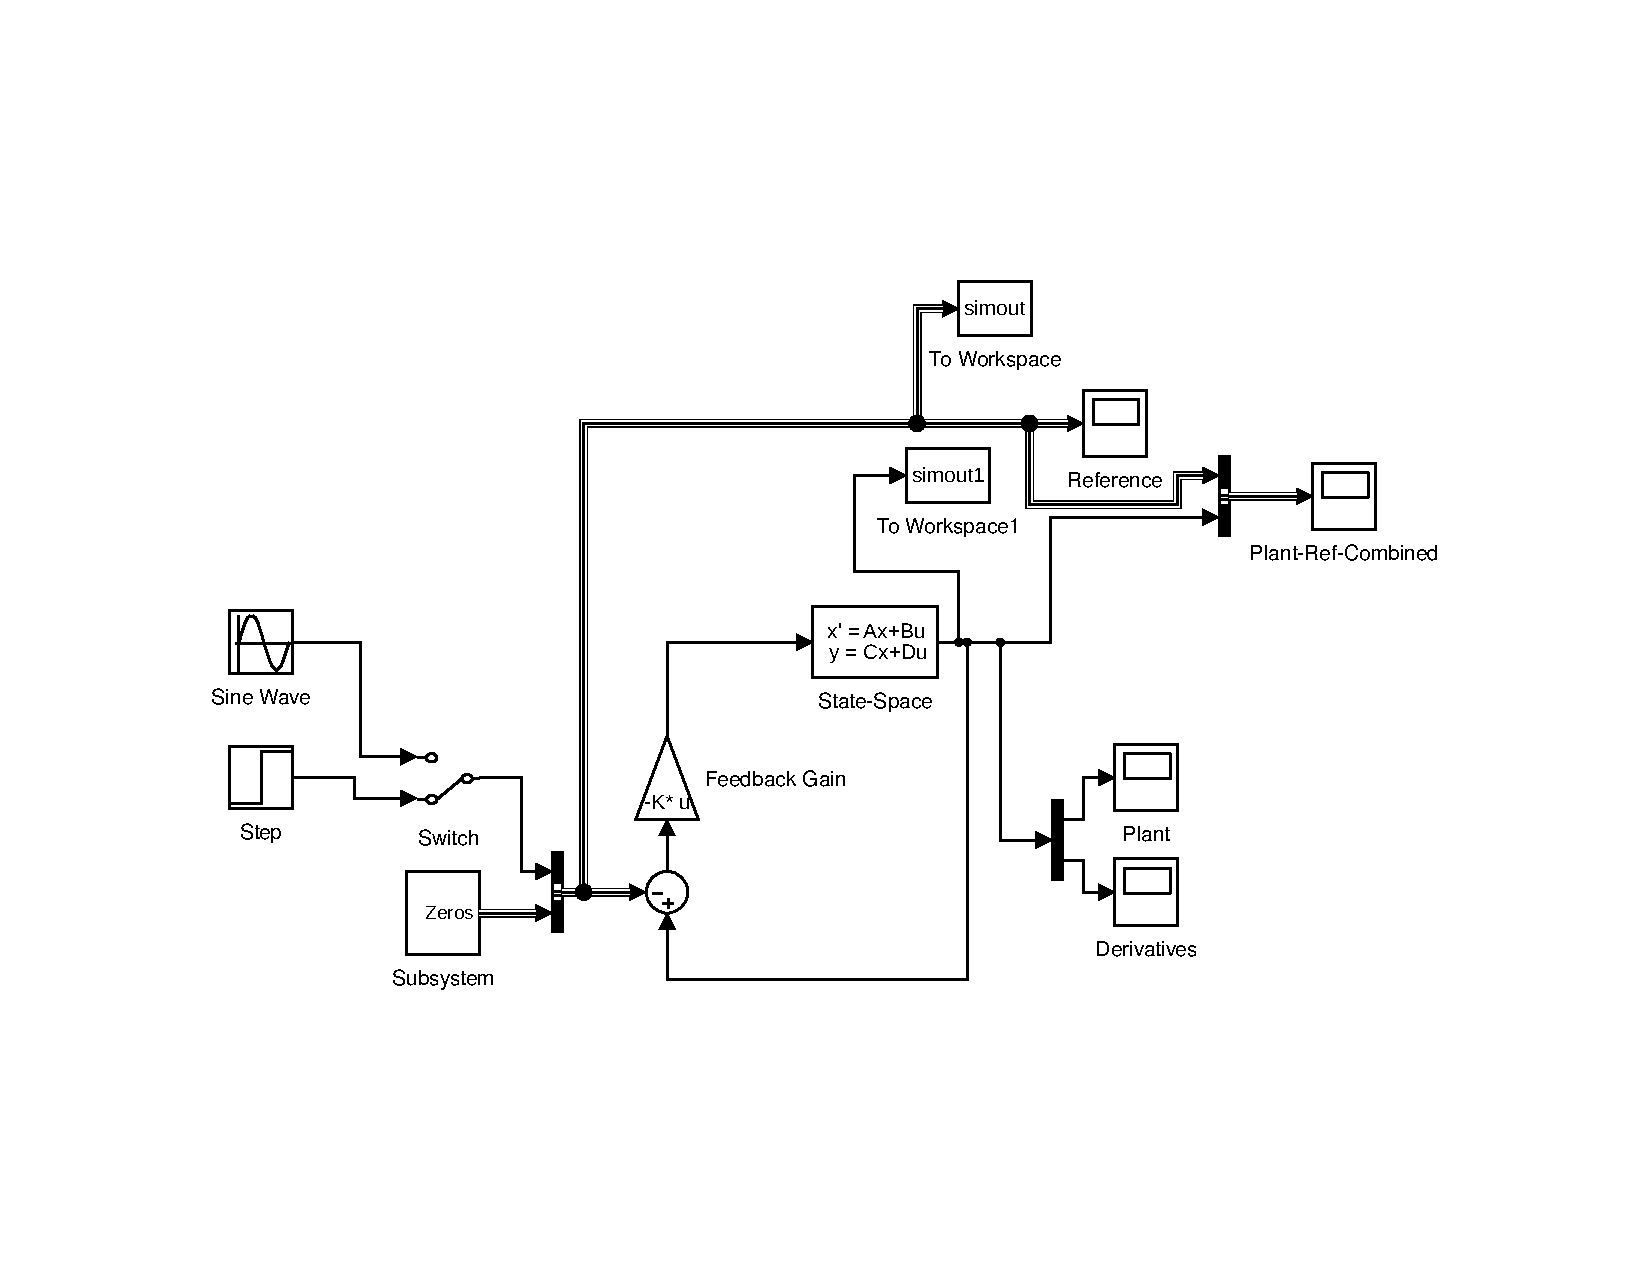
\includegraphics[scale=0.5]{images/simModelFullState.pdf}
\caption{The simulink Layout of our Simulation knowledge of all the states is assumed}
\label{fig:allStates}
\end{figure}
Figure~\ref{fig:allStates} shows our initial simulink diagram. The most important block in the control gain, that does the actual LQR-Control. The state space block in the center contains the continuous time system we showed in the previous section. In the left we have a selector that we use to choose between either a step or a sinusodial input. Below it we use a block of constant zeros to full up remaining entries of the input vector. 
As stated earlier we are using LQR-Control in this project. To compute the gain matrix for an LQR-Controller determines an state-feedback gain which minimizes the following cost function:
\begin{equation}
J = \int(\mathbf{x}^T Q \mathbf{x} + \mathbf{u}^T R \mathbf{u})dt.
\end{equation}
Initial but not optimal Q and R where given. \marginpar{Q = diag([350 1500 3 0.5]) for R = 10.} The $Q$ matrix gives weight to the different elements of the state vector. In our case hub position, arm position, angular hub and angular arm velocity. The R matrix, in our case a scalar makes the input more expensive. Our goals for tuning the controller are to achieve a satisfactory tracking for the hub angle $\theta$ without overshoot, while keeping the movement of the arm $\alpha$ as low as possible. At the same time we want to avoid actuator saturation. These are obviously conflicting objectives. So a good compromise is required. Figure~\ref{fig:stepResponse} shows the performance of the initially provided weighting parameters. From the tracking point of view the performance is not bad, however the input signal almost exceeds 5 Volts, which will might lead to actuator saturation if applied to the real plant. We chose the following weighting matrix to fix this problem:
\begin{equation}
\begin{pmatrix}
500 &		&	&	\\
	&1000	&	&	\\
	&	&3	&	\\
	&	&	&10	\\
\end{pmatrix}
\end{equation}
With the input weight $R = 30$. We increased the weight on the inputs to prevent saturation. As a higher input weight will make high inputs more expensive we expected this to fix our saturation problem. Furthermore it turns out more effective to penalize the acceleration of $\dot{\alpha}$ in comparison to a high value for $\alpha$. This is the case because we know that the reference for $\alpha$ will always be zero. Putting a higher weight on arm-acceleration prevents the arm from moving too fast away from its zero reference. In figure~{\ref{fig:stepResponse} on the right side we show the simulated behavior with our adapted weights, where the tracking remains comparably fast. 


\begin{figure}
%% This file was created by matlab2tikz v0.4.7 running on MATLAB 8.4.
% Copyright (c) 2008--2014, Nico Schlömer <nico.schloemer@gmail.com>
% All rights reserved.
% Minimal pgfplots version: 1.3
% 
% The latest updates can be retrieved from
%   http://www.mathworks.com/matlabcentral/fileexchange/22022-matlab2tikz
% where you can also make suggestions and rate matlab2tikz.
% 
\documentclass[tikz]{standalone}
\usepackage{pgfplots}
\usepackage{grffile}
\pgfplotsset{compat=newest}
\usetikzlibrary{plotmarks}
\usepackage{amsmath}

\begin{document}
%
% defining custom colors
\definecolor{mycolor1}{rgb}{0.00000,0.44700,0.74100}%
\definecolor{mycolor2}{rgb}{0.85000,0.32500,0.09800}%
\definecolor{mycolor3}{rgb}{0.92900,0.69400,0.12500}%
%
\begin{tikzpicture}

\begin{axis}[%
width=1.8in,
height=1in,
scale only axis,
separate axis lines,
every outer x axis line/.append style={white!15!black},
every x tick label/.append style={font=\color{white!15!black}},
xmin=0,
xmax=5,
every outer y axis line/.append style={white!15!black},
every y tick label/.append style={font=\color{white!15!black}},
ymin=-0.2,
ymax=0.8,
name=plot1,
%title style={font=\bfseries},
ylabel={plant, reference [rad]}
]
\addplot [color=mycolor1,solid,forget plot]
  table[row sep=crcr]{0	0\\
0.005	0\\
0.01	0\\
0.015	0\\
0.02	0\\
0.025	0\\
0.03	0\\
0.035	0\\
0.04	0\\
0.045	0\\
0.05	0\\
0.055	0\\
0.06	0\\
0.065	0\\
0.07	0\\
0.075	0\\
0.08	0\\
0.085	0\\
0.09	0\\
0.095	0\\
0.1	0\\
0.105	0\\
0.11	0\\
0.115	0\\
0.12	0\\
0.125	0\\
0.13	0\\
0.135	0\\
0.14	0\\
0.145	0\\
0.15	0\\
0.155	0\\
0.16	0\\
0.165	0\\
0.17	0\\
0.175	0\\
0.18	0\\
0.185	0\\
0.19	0\\
0.195	0\\
0.2	0\\
0.205	0\\
0.21	0\\
0.215	0\\
0.22	0\\
0.225	0\\
0.23	0\\
0.235	0\\
0.24	0\\
0.245	0\\
0.25	0\\
0.255	0\\
0.26	0\\
0.265	0\\
0.27	0\\
0.275	0\\
0.28	0\\
0.285	0\\
0.29	0\\
0.295	0\\
0.3	0\\
0.305	0\\
0.31	0\\
0.315	0\\
0.32	0\\
0.325	0\\
0.33	0\\
0.335	0\\
0.34	0\\
0.345	0\\
0.35	0\\
0.355	0\\
0.36	0\\
0.365	0\\
0.37	0\\
0.375	0\\
0.38	0\\
0.385	0\\
0.39	0\\
0.395	0\\
0.4	0\\
0.405	0\\
0.41	0\\
0.415	0\\
0.42	0\\
0.425	0\\
0.43	0\\
0.435	0\\
0.44	0\\
0.445	0\\
0.45	0\\
0.455	0\\
0.46	0\\
0.465	0\\
0.47	0\\
0.475	0\\
0.48	0\\
0.485	0\\
0.49	0\\
0.495	0\\
0.5	0\\
0.505	0\\
0.51	0\\
0.515	0\\
0.52	0\\
0.525	0\\
0.53	0\\
0.535	0\\
0.54	0\\
0.545	0\\
0.55	0\\
0.555	0\\
0.56	0\\
0.565	0\\
0.57	0\\
0.575	0\\
0.58	0\\
0.585	0\\
0.59	0\\
0.595	0\\
0.6	0\\
0.605	0\\
0.61	0\\
0.615	0\\
0.62	0\\
0.625	0\\
0.63	0\\
0.635	0\\
0.64	0\\
0.645	0\\
0.65	0\\
0.655	0\\
0.66	0\\
0.665	0\\
0.67	0\\
0.675	0\\
0.68	0\\
0.685	0\\
0.69	0\\
0.695	0\\
0.7	0\\
0.705	0\\
0.71	0\\
0.715	0\\
0.72	0\\
0.725	0\\
0.73	0\\
0.735	0\\
0.74	0\\
0.745	0\\
0.75	0\\
0.755	0\\
0.76	0\\
0.765	0\\
0.77	0\\
0.775	0\\
0.78	0\\
0.785	0\\
0.79	0\\
0.795	0\\
0.8	0\\
0.805	0\\
0.81	0\\
0.815	0\\
0.82	0\\
0.825	0\\
0.83	0\\
0.835	0\\
0.84	0\\
0.845	0\\
0.85	0\\
0.855	0\\
0.86	0\\
0.865	0\\
0.87	0\\
0.875	0\\
0.88	0\\
0.885	0\\
0.89	0\\
0.895	0\\
0.9	0\\
0.905	0\\
0.91	0\\
0.915	0\\
0.92	0\\
0.925	0\\
0.93	0\\
0.935	0\\
0.94	0\\
0.945	0\\
0.95	0\\
0.955	0\\
0.96	0\\
0.965	0\\
0.97	0\\
0.975	0\\
0.98	0\\
0.985	0\\
0.99	0\\
0.995	0\\
1	0\\
1.005	0.00523203624393392\\
1.01	0.018186605839208\\
1.015	0.0352342868591856\\
1.02	0.0539958675836227\\
1.025	0.0729538401874592\\
1.03	0.0911814985665003\\
1.035	0.108154164435518\\
1.04	0.123617771729083\\
1.045	0.137497513309732\\
1.05	0.149834471777402\\
1.055	0.160741798933166\\
1.06	0.170374551688914\\
1.065	0.178909067882093\\
1.07	0.18652900528233\\
1.075	0.193416032833595\\
1.08	0.199743767790938\\
1.085	0.205673974718829\\
1.09	0.211354337351883\\
1.095	0.216917320495604\\
1.1	0.222479783283137\\
1.105	0.228143105925134\\
1.11	0.233993662662367\\
1.115	0.240103523077566\\
1.12	0.24653129861244\\
1.125	0.253323075513464\\
1.13	0.260513392599091\\
1.135	0.268126234367861\\
1.14	0.276176018563894\\
1.145	0.284668563439095\\
1.15	0.293602024337562\\
1.155	0.302967792391718\\
1.16	0.312751350421486\\
1.165	0.322933082818445\\
1.17	0.333489037452368\\
1.175	0.344391638580611\\
1.18	0.355610350457881\\
1.185	0.367112291895478\\
1.19	0.378862802447752\\
1.195	0.39082596123959\\
1.2	0.402965059713482\\
1.205	0.415243029783715\\
1.21	0.427622829049477\\
1.215	0.440067784846418\\
1.22	0.452541899013558\\
1.225	0.465010115324052\\
1.23	0.477438551577801\\
1.235	0.489794698384265\\
1.24	0.502047586677305\\
1.245	0.514167926002721\\
1.25	0.526128215604857\\
1.255	0.537902830313022\\
1.26	0.54946808319269\\
1.265	0.560802266881934\\
1.27	0.571885675481361\\
1.275	0.582700608807132\\
1.28	0.593231360752331\\
1.285	0.603464193433073\\
1.29	0.613387298723041\\
1.295	0.6229907487045\\
1.3	0.632266436485938\\
1.305	0.641208008757046\\
1.31	0.649810791371382\\
1.315	0.658071709166338\\
1.32	0.665989201149497\\
1.325	0.673563132100536\\
1.33	0.680794701559025\\
1.335	0.687686351091074\\
1.34	0.694241670652191\\
1.345	0.700465304790197\\
1.35	0.706362859360872\\
1.355	0.711940809360391\\
1.36	0.717206408412709\\
1.365	0.722167600387061\\
1.37	0.726832933560775\\
1.375	0.731211477685625\\
1.38	0.735312744262281\\
1.385	0.739146610276779\\
1.39	0.74272324560561\\
1.395	0.746053044251857\\
1.4	0.749146559533802\\
1.405	0.752014443309568\\
1.41	0.754667389286558\\
1.415	0.757116080432633\\
1.42	0.759371140477116\\
1.425	0.76144308946361\\
1.43	0.763342303293271\\
1.435	0.765078977176455\\
1.44	0.766663092892383\\
1.445	0.768104389740616\\
1.45	0.769412339054492\\
1.455	0.770596122135182\\
1.46	0.771664611455526\\
1.465	0.772626354975165\\
1.47	0.773489563402598\\
1.475	0.774262100235515\\
1.48	0.774951474407985\\
1.485	0.77556483537163\\
1.49	0.776108970437781\\
1.495	0.776590304208553\\
1.5	0.777014899926774\\
1.505	0.777388462577599\\
1.51	0.777716343578334\\
1.515	0.77800354689743\\
1.52	0.77825473644863\\
1.525	0.778474244611791\\
1.53	0.77866608173794\\
1.535	0.778833946502436\\
1.54	0.778981236976806\\
1.545	0.779111062296642\\
1.55	0.779226254810009\\
1.555	0.779329382597903\\
1.56	0.779422762265478\\
1.565	0.779508471909898\\
1.57	0.779588364177768\\
1.575	0.779664079332135\\
1.58	0.77973705825588\\
1.585	0.779808555325088\\
1.59	0.779879651092488\\
1.595	0.779951264727374\\
1.6	0.780024166164523\\
1.605	0.780098987920441\\
1.61	0.780176236540865\\
1.615	0.780256303648721\\
1.62	0.780339476566789\\
1.625	0.780425948494016\\
1.63	0.780515828218898\\
1.635	0.780609149357447\\
1.64	0.780705879107156\\
1.645	0.780805926511913\\
1.65	0.780909150236081\\
1.655	0.781015365848986\\
1.66	0.781124352623757\\
1.665	0.781235859856914\\
1.67	0.781349612717323\\
1.675	0.78146531763506\\
1.68	0.781582667242469\\
1.685	0.781701344881166\\
1.69	0.781821028690034\\
1.695	0.781941395290304\\
1.7	0.782062123084725\\
1.705	0.78218289518849\\
1.71	0.782303402010148\\
1.715	0.782423343501092\\
1.72	0.782542431092445\\
1.725	0.782660389338271\\
1.73	0.782776957284001\\
1.735	0.782891889578862\\
1.74	0.783004957350819\\
1.745	0.783115948862261\\
1.75	0.78322466996424\\
1.755	0.783330944366603\\
1.76	0.783434613740823\\
1.765	0.783535537671783\\
1.77	0.783633593474079\\
1.775	0.783728675887817\\
1.78	0.783820696668139\\
1.785	0.783909584082021\\
1.79	0.783995282325145\\
1.795	0.784077750870941\\
1.8	0.784156963763106\\
1.805	0.784232908862202\\
1.81	0.784305587056185\\
1.815	0.784375011443996\\
1.82	0.78444120650061\\
1.825	0.784504207231271\\
1.83	0.784564058321931\\
1.835	0.784620813292271\\
1.84	0.784674533657029\\
1.845	0.784725288100765\\
1.85	0.784773151670588\\
1.855	0.784818204990824\\
1.86	0.784860533503076\\
1.865	0.784900226734607\\
1.87	0.784937377597525\\
1.875	0.784972081720795\\
1.88	0.785004436816686\\
1.885	0.785034542082893\\
1.89	0.785062497641197\\
1.895	0.785088404013206\\
1.9	0.785112361633437\\
1.905	0.785134470399696\\
1.91	0.785154829260488\\
1.915	0.785173535838968\\
1.92	0.785190686092727\\
1.925	0.785206374008561\\
1.93	0.78522069133119\\
1.935	0.785233727324798\\
1.94	0.785245568566103\\
1.945	0.78525629876764\\
1.95	0.785265998629796\\
1.955	0.785274745720137\\
1.96	0.785282614378482\\
1.965	0.785289675646162\\
1.97	0.7852959972179\\
1.975	0.785301643414729\\
1.98	0.785306675176356\\
1.985	0.785311150071437\\
1.99	0.785315122324208\\
1.995	0.785318642855978\\
2	0.785321759340015\\
2.005	0.78532451626841\\
2.01	0.785326955029534\\
2.015	0.785329113994788\\
2.02	0.785331028613374\\
2.025	0.78533273151389\\
2.03	0.78533425261161\\
2.035	0.785335619220382\\
2.04	0.785336856168125\\
2.045	0.785337985914983\\
2.05	0.785339028673272\\
2.055	0.785340002528383\\
2.06	0.785340923559915\\
2.065	0.78534180596234\\
2.07	0.785342662164581\\
2.075	0.785343502947937\\
2.08	0.785344337561857\\
2.085	0.785345173837105\\
2.09	0.785346018295934\\
2.095	0.785346876258912\\
2.1	0.78534775194812\\
2.105	0.785348648586466\\
2.11	0.785349568492922\\
2.115	0.785350513173509\\
2.12	0.785351483407917\\
2.125	0.785352479331678\\
2.13	0.785353500513823\\
2.135	0.785354546030014\\
2.14	0.785355614531151\\
2.145	0.785356704307484\\
2.15	0.78535781334829\\
2.155	0.78535893939718\\
2.16	0.785360080003136\\
2.165	0.785361232567392\\
2.17	0.785362394386272\\
2.175	0.785363562690125\\
2.18	0.785364734678508\\
2.185	0.785365907551767\\
2.19	0.785367078539178\\
2.195	0.785368244923816\\
2.2	0.785369404064316\\
2.205	0.785370553413718\\
2.21	0.785371690535539\\
2.215	0.785372813117282\\
2.22	0.785373918981522\\
2.225	0.785375006094763\\
2.23	0.785376072574228\\
2.235	0.785377116692744\\
2.24	0.785378136881882\\
2.245	0.785379131733512\\
2.25	0.785380099999932\\
2.255	0.785381040592688\\
2.26	0.785381952580263\\
2.265	0.785382835184734\\
2.27	0.785383687777546\\
2.275	0.785384509874504\\
2.28	0.78538530113012\\
2.285	0.785386061331391\\
2.29	0.785386790391139\\
2.295	0.785387488340977\\
2.3	0.785388155324007\\
2.305	0.785388791587321\\
2.31	0.785389397474376\\
2.315	0.785389973417313\\
2.32	0.785390519929282\\
2.325	0.785391037596823\\
2.33	0.785391527072348\\
2.335	0.785391989066783\\
2.34	0.785392424342393\\
2.345	0.78539283370582\\
2.35	0.785393218001386\\
2.355	0.785393578104653\\
2.36	0.785393914916288\\
2.365	0.785394229356231\\
2.37	0.785394522358185\\
2.375	0.785394794864438\\
2.38	0.785395047821019\\
2.385	0.785395282173194\\
2.39	0.785395498861305\\
2.395	0.785395698816941\\
2.4	0.78539588295945\\
2.405	0.785396052192773\\
2.41	0.785396207402604\\
2.415	0.785396349453858\\
2.42	0.785396479188447\\
2.425	0.785396597423339\\
2.43	0.785396704948898\\
2.435	0.785396802527497\\
2.44	0.785396890892372\\
2.445	0.785396970746724\\
2.45	0.785397042763039\\
2.455	0.785397107582619\\
2.46	0.785397165815315\\
2.465	0.78539721803943\\
2.47	0.785397264801799\\
2.475	0.785397306618015\\
2.48	0.7853973439728\\
2.485	0.785397377320492\\
2.49	0.785397407085656\\
2.495	0.785397433663786\\
2.5	0.785397457422097\\
2.505	0.785397478700395\\
2.51	0.785397497812007\\
2.515	0.785397515044773\\
2.52	0.785397530662071\\
2.525	0.785397544903887\\
2.53	0.785397557987906\\
2.535	0.785397570110621\\
2.54	0.785397581448456\\
2.545	0.785397592158884\\
2.55	0.785397602381552\\
2.555	0.785397612239389\\
2.56	0.785397621839705\\
2.565	0.785397631275267\\
2.57	0.785397640625354\\
2.575	0.785397649956785\\
2.58	0.785397659324914\\
2.585	0.7853976687746\\
2.59	0.785397678341126\\
2.595	0.785397688051099\\
2.6	0.785397697923299\\
2.605	0.785397707969492\\
2.61	0.785397718195201\\
2.615	0.785397728600433\\
2.62	0.785397739180374\\
2.625	0.78539774992603\\
2.63	0.785397760824829\\
2.635	0.785397771861194\\
2.64	0.785397783017055\\
2.645	0.78539779427234\\
2.65	0.785397805605418\\
2.655	0.785397816993503\\
2.66	0.785397828413028\\
2.665	0.785397839839982\\
2.67	0.785397851250207\\
2.675	0.785397862619673\\
2.68	0.785397873924715\\
2.685	0.785397885142243\\
2.69	0.785397896249929\\
2.695	0.785397907226357\\
2.7	0.785397918051163\\
2.705	0.785397928705142\\
2.71	0.785397939170336\\
2.715	0.785397949430106\\
2.72	0.785397959469181\\
2.725	0.785397969273698\\
2.73	0.785397978831216\\
2.735	0.785397988130727\\
2.74	0.78539799716265\\
2.745	0.785398005918811\\
2.75	0.78539801439242\\
2.755	0.785398022578034\\
2.76	0.785398030471516\\
2.765	0.785398038069983\\
2.77	0.785398045371758\\
2.775	0.785398052376303\\
2.78	0.785398059084163\\
2.785	0.785398065496899\\
2.79	0.78539807161702\\
2.795	0.785398077447913\\
2.8	0.78539808299378\\
2.805	0.78539808825956\\
2.81	0.785398093250866\\
2.815	0.785398097973915\\
2.82	0.78539810243546\\
2.825	0.785398106642725\\
2.83	0.785398110603344\\
2.835	0.785398114325294\\
2.84	0.785398117816842\\
2.845	0.785398121086484\\
2.85	0.785398124142895\\
2.855	0.785398126994876\\
2.86	0.785398129651306\\
2.865	0.785398132121101\\
2.87	0.785398134413167\\
2.875	0.785398136536364\\
2.88	0.785398138499473\\
2.885	0.785398140311161\\
2.89	0.785398141979949\\
2.895	0.785398143514191\\
2.9	0.785398144922048\\
2.905	0.785398146211468\\
2.91	0.785398147390164\\
2.915	0.785398148465604\\
2.92	0.785398149444996\\
2.925	0.785398150335274\\
2.93	0.785398151143095\\
2.935	0.785398151874828\\
2.94	0.785398152536551\\
2.945	0.785398153134051\\
2.95	0.785398153672817\\
2.955	0.785398154158047\\
2.96	0.785398154594644\\
2.965	0.785398154987226\\
2.97	0.785398155340123\\
2.975	0.785398155657388\\
2.98	0.785398155942801\\
2.985	0.785398156199878\\
2.99	0.785398156431877\\
2.995	0.785398156641805\\
3	0.785398156832434\\
3.005	0.785398157006303\\
3.01	0.78539815716573\\
3.015	0.785398157312826\\
3.02	0.7853981574495\\
3.025	0.785398157577471\\
3.03	0.78539815769828\\
3.035	0.785398157813301\\
3.04	0.785398157923745\\
3.045	0.785398158030681\\
3.05	0.785398158135034\\
3.055	0.785398158237605\\
3.06	0.785398158339074\\
3.065	0.785398158440012\\
3.07	0.785398158540892\\
3.075	0.785398158642092\\
3.08	0.785398158743908\\
3.085	0.785398158846562\\
3.09	0.785398158950206\\
3.095	0.785398159054932\\
3.1	0.785398159160781\\
3.105	0.785398159267743\\
3.11	0.78539815937577\\
3.115	0.785398159484776\\
3.12	0.785398159594648\\
3.125	0.785398159705247\\
3.13	0.78539815981641\\
3.135	0.785398159927963\\
3.14	0.785398160039717\\
3.145	0.785398160151473\\
3.15	0.785398160263029\\
3.155	0.785398160374178\\
3.16	0.785398160484713\\
3.165	0.785398160594431\\
3.17	0.785398160703132\\
3.175	0.785398160810621\\
3.18	0.785398160916711\\
3.185	0.785398161021225\\
3.19	0.785398161123993\\
3.195	0.78539816122486\\
3.2	0.785398161323678\\
3.205	0.785398161420315\\
3.21	0.785398161514647\\
3.215	0.785398161606566\\
3.22	0.785398161695977\\
3.225	0.785398161782794\\
3.23	0.785398161866948\\
3.235	0.785398161948379\\
3.24	0.785398162027042\\
3.245	0.785398162102901\\
3.25	0.785398162175934\\
3.255	0.785398162246127\\
3.26	0.785398162313479\\
3.265	0.785398162377998\\
3.27	0.7853981624397\\
3.275	0.785398162498611\\
3.28	0.785398162554765\\
3.285	0.785398162608202\\
3.29	0.785398162658971\\
3.295	0.785398162707125\\
3.3	0.785398162752723\\
3.305	0.785398162795831\\
3.31	0.785398162836516\\
3.315	0.785398162874852\\
3.32	0.785398162910913\\
3.325	0.785398162944777\\
3.33	0.785398162976526\\
3.335	0.785398163006241\\
3.34	0.785398163034005\\
3.345	0.785398163059902\\
3.35	0.785398163084015\\
3.355	0.78539816310643\\
3.36	0.785398163127229\\
3.365	0.785398163146496\\
3.37	0.785398163164312\\
3.375	0.785398163180758\\
3.38	0.785398163195912\\
3.385	0.785398163209851\\
3.39	0.785398163222652\\
3.395	0.785398163234386\\
3.4	0.785398163245124\\
3.405	0.785398163254934\\
3.41	0.785398163263882\\
3.415	0.785398163272031\\
3.42	0.785398163279442\\
3.425	0.785398163286172\\
3.43	0.785398163292275\\
3.435	0.785398163297805\\
3.44	0.78539816330281\\
3.445	0.785398163307338\\
3.45	0.785398163311431\\
3.455	0.785398163315132\\
3.46	0.785398163318479\\
3.465	0.785398163321509\\
3.47	0.785398163324254\\
3.475	0.785398163326747\\
3.48	0.785398163329016\\
3.485	0.785398163331087\\
3.49	0.785398163332986\\
3.495	0.785398163334735\\
3.5	0.785398163336353\\
3.505	0.78539816333786\\
3.51	0.785398163339273\\
3.515	0.785398163340606\\
3.52	0.785398163341873\\
3.525	0.785398163343086\\
3.53	0.785398163344255\\
3.535	0.78539816334539\\
3.54	0.785398163346499\\
3.545	0.785398163347589\\
3.55	0.785398163348665\\
3.555	0.785398163349732\\
3.56	0.785398163350795\\
3.565	0.785398163351857\\
3.57	0.785398163352919\\
3.575	0.785398163353985\\
3.58	0.785398163355055\\
3.585	0.78539816335613\\
3.59	0.785398163357211\\
3.595	0.785398163358296\\
3.6	0.785398163359386\\
3.605	0.785398163360481\\
3.61	0.785398163361578\\
3.615	0.785398163362676\\
3.62	0.785398163363775\\
3.625	0.785398163364873\\
3.63	0.785398163365968\\
3.635	0.785398163367058\\
3.64	0.785398163368142\\
3.645	0.785398163369219\\
3.65	0.785398163370285\\
3.655	0.785398163371339\\
3.66	0.785398163372381\\
3.665	0.785398163373408\\
3.67	0.785398163374418\\
3.675	0.78539816337541\\
3.68	0.785398163376384\\
3.685	0.785398163377337\\
3.69	0.785398163378268\\
3.695	0.785398163379176\\
3.7	0.785398163380061\\
3.705	0.785398163380922\\
3.71	0.785398163381757\\
3.715	0.785398163382567\\
3.72	0.78539816338335\\
3.725	0.785398163384107\\
3.73	0.785398163384836\\
3.735	0.785398163385539\\
3.74	0.785398163386214\\
3.745	0.785398163386863\\
3.75	0.785398163387484\\
3.755	0.785398163388078\\
3.76	0.785398163388645\\
3.765	0.785398163389186\\
3.77	0.785398163389702\\
3.775	0.785398163390191\\
3.78	0.785398163390656\\
3.785	0.785398163391097\\
3.79	0.785398163391513\\
3.795	0.785398163391907\\
3.8	0.785398163392278\\
3.805	0.785398163392628\\
3.81	0.785398163392956\\
3.815	0.785398163393265\\
3.82	0.785398163393554\\
3.825	0.785398163393824\\
3.83	0.785398163394077\\
3.835	0.785398163394312\\
3.84	0.785398163394531\\
3.845	0.785398163394735\\
3.85	0.785398163394924\\
3.855	0.785398163395099\\
3.86	0.785398163395261\\
3.865	0.785398163395411\\
3.87	0.785398163395548\\
3.875	0.785398163395675\\
3.88	0.785398163395792\\
3.885	0.785398163395899\\
3.89	0.785398163395997\\
3.895	0.785398163396087\\
3.9	0.785398163396169\\
3.905	0.785398163396244\\
3.91	0.785398163396312\\
3.915	0.785398163396374\\
3.92	0.785398163396431\\
3.925	0.785398163396482\\
3.93	0.785398163396529\\
3.935	0.785398163396571\\
3.94	0.78539816339661\\
3.945	0.785398163396645\\
3.95	0.785398163396676\\
3.955	0.785398163396705\\
3.96	0.785398163396732\\
3.965	0.785398163396756\\
3.97	0.785398163396778\\
3.975	0.785398163396799\\
3.98	0.785398163396818\\
3.985	0.785398163396835\\
3.99	0.785398163396852\\
3.995	0.785398163396867\\
4	0.785398163396881\\
4.005	0.785398163396895\\
4.01	0.785398163396908\\
4.015	0.785398163396921\\
4.02	0.785398163396933\\
4.025	0.785398163396945\\
4.03	0.785398163396956\\
4.035	0.785398163396968\\
4.04	0.785398163396979\\
4.045	0.78539816339699\\
4.05	0.785398163397001\\
4.055	0.785398163397012\\
4.06	0.785398163397023\\
4.065	0.785398163397034\\
4.07	0.785398163397045\\
4.075	0.785398163397056\\
4.08	0.785398163397066\\
4.085	0.785398163397077\\
4.09	0.785398163397088\\
4.095	0.785398163397099\\
4.1	0.78539816339711\\
4.105	0.785398163397121\\
4.11	0.785398163397132\\
4.115	0.785398163397142\\
4.12	0.785398163397153\\
4.125	0.785398163397164\\
4.13	0.785398163397174\\
4.135	0.785398163397184\\
4.14	0.785398163397195\\
4.145	0.785398163397205\\
4.15	0.785398163397215\\
4.155	0.785398163397225\\
4.16	0.785398163397234\\
4.165	0.785398163397244\\
4.17	0.785398163397253\\
4.175	0.785398163397262\\
4.18	0.785398163397271\\
4.185	0.785398163397279\\
4.19	0.785398163397288\\
4.195	0.785398163397296\\
4.2	0.785398163397303\\
4.205	0.785398163397311\\
4.21	0.785398163397318\\
4.215	0.785398163397325\\
4.22	0.785398163397332\\
4.225	0.785398163397339\\
4.23	0.785398163397345\\
4.235	0.785398163397351\\
4.24	0.785398163397357\\
4.245	0.785398163397362\\
4.25	0.785398163397367\\
4.255	0.785398163397372\\
4.26	0.785398163397377\\
4.265	0.785398163397381\\
4.27	0.785398163397386\\
4.275	0.78539816339739\\
4.28	0.785398163397393\\
4.285	0.785398163397397\\
4.29	0.7853981633974\\
4.295	0.785398163397404\\
4.3	0.785398163397407\\
4.305	0.785398163397409\\
4.31	0.785398163397412\\
4.315	0.785398163397415\\
4.32	0.785398163397417\\
4.325	0.785398163397419\\
4.33	0.785398163397421\\
4.335	0.785398163397423\\
4.34	0.785398163397425\\
4.345	0.785398163397426\\
4.35	0.785398163397428\\
4.355	0.785398163397429\\
4.36	0.78539816339743\\
4.365	0.785398163397431\\
4.37	0.785398163397432\\
4.375	0.785398163397433\\
4.38	0.785398163397434\\
4.385	0.785398163397435\\
4.39	0.785398163397436\\
4.395	0.785398163397437\\
4.4	0.785398163397437\\
4.405	0.785398163397438\\
4.41	0.785398163397438\\
4.415	0.785398163397439\\
4.42	0.785398163397439\\
4.425	0.78539816339744\\
4.43	0.78539816339744\\
4.435	0.78539816339744\\
4.44	0.785398163397441\\
4.445	0.785398163397441\\
4.45	0.785398163397441\\
4.455	0.785398163397441\\
4.46	0.785398163397442\\
4.465	0.785398163397442\\
4.47	0.785398163397442\\
4.475	0.785398163397442\\
4.48	0.785398163397442\\
4.485	0.785398163397443\\
4.49	0.785398163397443\\
4.495	0.785398163397443\\
4.5	0.785398163397443\\
4.505	0.785398163397443\\
4.51	0.785398163397443\\
4.515	0.785398163397443\\
4.52	0.785398163397443\\
4.525	0.785398163397443\\
4.53	0.785398163397444\\
4.535	0.785398163397444\\
4.54	0.785398163397444\\
4.545	0.785398163397444\\
4.55	0.785398163397444\\
4.555	0.785398163397444\\
4.56	0.785398163397444\\
4.565	0.785398163397444\\
4.57	0.785398163397444\\
4.575	0.785398163397445\\
4.58	0.785398163397445\\
4.585	0.785398163397445\\
4.59	0.785398163397445\\
4.595	0.785398163397445\\
4.6	0.785398163397445\\
4.605	0.785398163397445\\
4.61	0.785398163397445\\
4.615	0.785398163397445\\
4.62	0.785398163397446\\
4.625	0.785398163397446\\
4.63	0.785398163397446\\
4.635	0.785398163397446\\
4.64	0.785398163397446\\
4.645	0.785398163397446\\
4.65	0.785398163397446\\
4.655	0.785398163397446\\
4.66	0.785398163397446\\
4.665	0.785398163397447\\
4.67	0.785398163397447\\
4.675	0.785398163397447\\
4.68	0.785398163397447\\
4.685	0.785398163397447\\
4.69	0.785398163397447\\
4.695	0.785398163397447\\
4.7	0.785398163397447\\
4.705	0.785398163397447\\
4.71	0.785398163397448\\
4.715	0.785398163397448\\
4.72	0.785398163397448\\
4.725	0.785398163397448\\
4.73	0.785398163397448\\
4.735	0.785398163397448\\
4.74	0.785398163397448\\
4.745	0.785398163397448\\
4.75	0.785398163397448\\
4.755	0.785398163397448\\
4.76	0.785398163397448\\
4.765	0.785398163397448\\
4.77	0.785398163397448\\
4.775	0.785398163397448\\
4.78	0.785398163397448\\
4.785	0.785398163397448\\
4.79	0.785398163397448\\
4.795	0.785398163397448\\
4.8	0.785398163397448\\
4.805	0.785398163397448\\
4.81	0.785398163397448\\
4.815	0.785398163397448\\
4.82	0.785398163397448\\
4.825	0.785398163397448\\
4.83	0.785398163397448\\
4.835	0.785398163397448\\
4.84	0.785398163397448\\
4.845	0.785398163397448\\
4.85	0.785398163397448\\
4.855	0.785398163397448\\
4.86	0.785398163397448\\
4.865	0.785398163397448\\
4.87	0.785398163397448\\
4.875	0.785398163397448\\
4.88	0.785398163397448\\
4.885	0.785398163397448\\
4.89	0.785398163397448\\
4.895	0.785398163397448\\
4.9	0.785398163397448\\
4.905	0.785398163397448\\
4.91	0.785398163397448\\
4.915	0.785398163397448\\
4.92	0.785398163397448\\
4.925	0.785398163397448\\
4.93	0.785398163397448\\
4.935	0.785398163397448\\
4.94	0.785398163397448\\
4.945	0.785398163397448\\
4.95	0.785398163397448\\
4.955	0.785398163397448\\
4.96	0.785398163397448\\
4.965	0.785398163397448\\
4.97	0.785398163397448\\
4.975	0.785398163397448\\
4.98	0.785398163397448\\
4.985	0.785398163397448\\
4.99	0.785398163397448\\
4.995	0.785398163397448\\
5	0.785398163397448\\
};
\addplot [color=mycolor2,solid,forget plot]
  table[row sep=crcr]{0	0\\
0.005	0\\
0.01	0\\
0.015	0\\
0.02	0\\
0.025	0\\
0.03	0\\
0.035	0\\
0.04	0\\
0.045	0\\
0.05	0\\
0.055	0\\
0.06	0\\
0.065	0\\
0.07	0\\
0.075	0\\
0.08	0\\
0.085	0\\
0.09	0\\
0.095	0\\
0.1	0\\
0.105	0\\
0.11	0\\
0.115	0\\
0.12	0\\
0.125	0\\
0.13	0\\
0.135	0\\
0.14	0\\
0.145	0\\
0.15	0\\
0.155	0\\
0.16	0\\
0.165	0\\
0.17	0\\
0.175	0\\
0.18	0\\
0.185	0\\
0.19	0\\
0.195	0\\
0.2	0\\
0.205	0\\
0.21	0\\
0.215	0\\
0.22	0\\
0.225	0\\
0.23	0\\
0.235	0\\
0.24	0\\
0.245	0\\
0.25	0\\
0.255	0\\
0.26	0\\
0.265	0\\
0.27	0\\
0.275	0\\
0.28	0\\
0.285	0\\
0.29	0\\
0.295	0\\
0.3	0\\
0.305	0\\
0.31	0\\
0.315	0\\
0.32	0\\
0.325	0\\
0.33	0\\
0.335	0\\
0.34	0\\
0.345	0\\
0.35	0\\
0.355	0\\
0.36	0\\
0.365	0\\
0.37	0\\
0.375	0\\
0.38	0\\
0.385	0\\
0.39	0\\
0.395	0\\
0.4	0\\
0.405	0\\
0.41	0\\
0.415	0\\
0.42	0\\
0.425	0\\
0.43	0\\
0.435	0\\
0.44	0\\
0.445	0\\
0.45	0\\
0.455	0\\
0.46	0\\
0.465	0\\
0.47	0\\
0.475	0\\
0.48	0\\
0.485	0\\
0.49	0\\
0.495	0\\
0.5	0\\
0.505	0\\
0.51	0\\
0.515	0\\
0.52	0\\
0.525	0\\
0.53	0\\
0.535	0\\
0.54	0\\
0.545	0\\
0.55	0\\
0.555	0\\
0.56	0\\
0.565	0\\
0.57	0\\
0.575	0\\
0.58	0\\
0.585	0\\
0.59	0\\
0.595	0\\
0.6	0\\
0.605	0\\
0.61	0\\
0.615	0\\
0.62	0\\
0.625	0\\
0.63	0\\
0.635	0\\
0.64	0\\
0.645	0\\
0.65	0\\
0.655	0\\
0.66	0\\
0.665	0\\
0.67	0\\
0.675	0\\
0.68	0\\
0.685	0\\
0.69	0\\
0.695	0\\
0.7	0\\
0.705	0\\
0.71	0\\
0.715	0\\
0.72	0\\
0.725	0\\
0.73	0\\
0.735	0\\
0.74	0\\
0.745	0\\
0.75	0\\
0.755	0\\
0.76	0\\
0.765	0\\
0.77	0\\
0.775	0\\
0.78	0\\
0.785	0\\
0.79	0\\
0.795	0\\
0.8	0\\
0.805	0\\
0.81	0\\
0.815	0\\
0.82	0\\
0.825	0\\
0.83	0\\
0.835	0\\
0.84	0\\
0.845	0\\
0.85	0\\
0.855	0\\
0.86	0\\
0.865	0\\
0.87	0\\
0.875	0\\
0.88	0\\
0.885	0\\
0.89	0\\
0.895	0\\
0.9	0\\
0.905	0\\
0.91	0\\
0.915	0\\
0.92	0\\
0.925	0\\
0.93	0\\
0.935	0\\
0.94	0\\
0.945	0\\
0.95	0\\
0.955	0\\
0.96	0\\
0.965	0\\
0.97	0\\
0.975	0\\
0.98	0\\
0.985	0\\
0.99	0\\
0.995	0\\
1	0\\
1.005	-0.00522895785388764\\
1.01	-0.018140478443417\\
1.015	-0.0350192359012344\\
1.02	-0.0533723828618899\\
1.025	-0.0715582452015607\\
1.03	-0.0885267561879355\\
1.035	-0.103637942408965\\
1.04	-0.116534941998379\\
1.045	-0.127055133947732\\
1.05	-0.13516791251939\\
1.055	-0.140931099966631\\
1.06	-0.144460405602637\\
1.065	-0.145908025051329\\
1.07	-0.145447650376318\\
1.075	-0.143263983380385\\
1.08	-0.139545417965598\\
1.085	-0.134478957925612\\
1.09	-0.128246716180759\\
1.095	-0.121023536753933\\
1.1	-0.112975417194006\\
1.105	-0.104258504464883\\
1.11	-0.0950185039444863\\
1.115	-0.085390387782719\\
1.12	-0.075498321498049\\
1.125	-0.065455750569575\\
1.13	-0.05536560485087\\
1.135	-0.0453205899492992\\
1.14	-0.0354035427141649\\
1.145	-0.0256878336598002\\
1.15	-0.0162378032135887\\
1.155	-0.00710922161080584\\
1.16	0.00165023560250704\\
1.165	0.010000502913985\\
1.17	0.0179086362997285\\
1.175	0.0253483251363851\\
1.18	0.0322994081977014\\
1.185	0.0387473967836846\\
1.19	0.0446830075534548\\
1.195	0.050101707230963\\
1.2	0.0550032710072106\\
1.205	0.0593913561604853\\
1.21	0.0632730921482778\\
1.215	0.0666586881846732\\
1.22	0.0695610591005942\\
1.225	0.0719954700881671\\
1.23	0.0739792007523578\\
1.235	0.0755312287312077\\
1.24	0.0766719329991639\\
1.245	0.0774228168351487\\
1.25	0.077806250317273\\
1.255	0.0778452320987489\\
1.26	0.0775631701239369\\
1.265	0.0769836808589477\\
1.27	0.0761304065372328\\
1.275	0.0750268498565632\\
1.28	0.0736962255091572\\
1.285	0.0721613278809166\\
1.29	0.0704444142182274\\
1.295	0.0685671025310246\\
1.3	0.0665502834782807\\
1.305	0.0644140454662276\\
1.31	0.0621776121799352\\
1.315	0.0598592917648495\\
1.32	0.0574764368760328\\
1.325	0.0550454148186787\\
1.33	0.0525815870135168\\
1.335	0.050099297034544\\
1.34	0.0476118664836674\\
1.345	0.0451315979869408\\
1.35	0.0426697846196868\\
1.355	0.040236725092595\\
1.36	0.0378417440574819\\
1.365	0.0354932169194905\\
1.37	0.0331985985717686\\
1.375	0.0309644554988204\\
1.38	0.0287965007254971\\
1.385	0.0266996311197464\\
1.39	0.024677966588538\\
1.395	0.0227348907376277\\
1.4	0.0208730925968228\\
1.405	0.0190946090430017\\
1.41	0.0174008675831654\\
1.415	0.0157927291891357\\
1.42	0.0142705309040324\\
1.425	0.0128341279682704\\
1.43	0.0114829352394329\\
1.435	0.0102159677059116\\
1.44	0.00903187991861981\\
1.445	0.00792900418831761\\
1.45	0.00690538741811721\\
1.455	0.00595882646152252\\
1.46	0.00508690191590359\\
1.465	0.00428701027958973\\
1.47	0.00355639441780429\\
1.475	0.00289217229845534\\
1.48	0.00229136397336926\\
1.485	0.00175091679392058\\
1.49	0.00126772886220925\\
1.495	0.000838670729990192\\
1.5	0.000460605367513933\\
1.505	0.000130406433325272\\
1.51	-0.000155025116062033\\
1.515	-0.000398746030802024\\
1.52	-0.000603757334882442\\
1.525	-0.000772992398947669\\
1.53	-0.000909306457643734\\
1.535	-0.00101546750686727\\
1.54	-0.00109414851354394\\
1.545	-0.00114792086848412\\
1.55	-0.0011792490114134\\
1.555	-0.00119048615640405\\
1.56	-0.00118387104559331\\
1.565	-0.00116152565921731\\
1.57	-0.00112545381057102\\
1.575	-0.0010775405554796\\
1.58	-0.00101955234719334\\
1.585	-0.000953137869255918\\
1.59	-0.000879829480804382\\
1.595	-0.000801045210903526\\
1.6	-0.000718091240860391\\
1.605	-0.000632164815974939\\
1.61	-0.000544357530828262\\
1.615	-0.000455658934961978\\
1.62	-0.000366960408633781\\
1.625	-0.000279059261220454\\
1.63	-0.000192663007756881\\
1.635	-0.00010839378202775\\
1.64	-2.67928475473982e-05\\
1.645	5.16748293437829e-05\\
1.65	0.00012661597718731\\
1.655	0.000197704418044603\\
1.66	0.000264676494463935\\
1.665	0.000327326549526926\\
1.67	0.000385502482165339\\
1.675	0.000439101397474669\\
1.68	0.000488065369389493\\
1.685	0.000532377330831662\\
1.69	0.000572057104300409\\
1.695	0.000607157583846495\\
1.7	0.000637761077462436\\
1.705	0.000663975817129083\\
1.71	0.000685932642085354\\
1.715	0.000703781859332588\\
1.72	0.00071769028394636\\
1.725	0.000727838460445189\\
1.73	0.000734418065254711\\
1.735	0.000737629489205171\\
1.74	0.000737679598005856\\
1.745	0.00073477966774909\\
1.75	0.000729143491704521\\
1.755	0.000720985653967529\\
1.76	0.000710519964919358\\
1.765	0.000697958052936402\\
1.77	0.000683508106347346\\
1.775	0.000667373759274831\\
1.78	0.000649753114708248\\
1.785	0.000630837897931253\\
1.79	0.000610812733267104\\
1.795	0.00058985453700194\\
1.8	0.000568132019296366\\
1.805	0.000545805287894259\\
1.81	0.000523025546480496\\
1.815	0.000499934880621796\\
1.82	0.000476666124342988\\
1.825	0.000453342800540877\\
1.83	0.000430079128615461\\
1.835	0.000406980092900161\\
1.84	0.000384141565695272\\
1.845	0.000361650478948966\\
1.85	0.000339585038884632\\
1.855	0.00031801497813937\\
1.86	0.000297001840253286\\
1.865	0.000276599291630453\\
1.87	0.000256853456377559\\
1.875	0.000237803269713471\\
1.88	0.000219480845929935\\
1.885	0.000201911857169036\\
1.89	0.000185115919564872\\
1.895	0.000169106983574085\\
1.9	0.000153893725590889\\
1.905	0.000139479938206159\\
1.91	0.000125864916725852\\
1.915	0.000113043839810828\\
1.92	0.000101008142337247\\
1.925	8.97458788036334e-05\\
1.93	7.92420758268851e-05\\
1.935	6.94790724747008e-05\\
1.94	6.04368473758028e-05\\
1.945	5.20933317317828e-05\\
1.95	4.44247075253877e-05\\
1.955	3.7405690379495e-05\\
1.96	3.10097966690984e-05\\
1.965	2.52095946253563e-05\\
1.97	1.99769392964517e-05\\
1.975	1.52831913448312e-05\\
1.98	1.10994197646934e-05\\
1.985	7.39658869765424e-06\\
1.99	4.14572860874558e-06\\
1.995	1.3180921596412e-06\\
2	-1.11470481829113e-06\\
2.005	-3.1805567914457e-06\\
2.01	-4.90675592337885e-06\\
2.015	-6.31989285642853e-06\\
2.02	-7.44577029192835e-06\\
2.025	-8.30932875829054e-06\\
2.03	-8.93458393548776e-06\\
2.035	-9.34457488959651e-06\\
2.04	-9.56132256163179e-06\\
2.045	-9.60579785045646e-06\\
2.05	-9.4978986296658e-06\\
2.055	-9.25643504258787e-06\\
2.06	-8.89912242750725e-06\\
2.065	-8.44258123651733e-06\\
2.07	-7.90234332565646e-06\\
2.075	-7.29286401081823e-06\\
2.08	-6.62753930300769e-06\\
2.085	-5.91872775751857e-06\\
2.09	-5.17777639421245e-06\\
2.095	-4.41505017000997e-06\\
2.1	-3.63996450968845e-06\\
2.105	-2.86102042684733e-06\\
2.11	-2.08584179324216e-06\\
2.115	-1.32121434136566e-06\\
2.12	-5.7312601198452e-07\\
2.125	1.53191714867308e-07\\
2.13	8.53221840343087e-07\\
2.135	1.52311952734204e-06\\
2.14	2.15966972405513e-06\\
2.145	2.76024498820731e-06\\
2.15	3.32276374522458e-06\\
2.155	3.84564918986133e-06\\
2.16	4.32778901798844e-06\\
2.165	4.76849615333599e-06\\
2.17	5.16747061305015e-06\\
2.175	5.52476263601e-06\\
2.18	5.84073717897642e-06\\
2.185	6.11603986784472e-06\\
2.19	6.35156447455492e-06\\
2.195	6.54842197458073e-06\\
2.2	6.70791122536605e-06\\
2.205	6.83149129259926e-06\\
2.21	6.92075543880555e-06\\
2.215	6.97740677735988e-06\\
2.22	7.00323558466241e-06\\
2.225	7.0000982538451e-06\\
2.23	6.96989786495623e-06\\
2.235	6.91456633907399e-06\\
2.24	6.83604813718026e-06\\
2.245	6.73628545884811e-06\\
2.25	6.61720489082249e-06\\
2.255	6.48070545135595e-06\\
2.26	6.32864797265922e-06\\
2.265	6.16284576099659e-06\\
2.27	5.98505647175259e-06\\
2.275	5.79697513517687e-06\\
2.28	5.60022826743396e-06\\
2.285	5.39636900100655e-06\\
2.29	5.18687316837395e-06\\
2.295	4.97313627317815e-06\\
2.3	4.75647128375359e-06\\
2.305	4.53810718490019e-06\\
2.31	4.31918822508032e-06\\
2.315	4.10077379778671e-06\\
2.32	3.88383889762658e-06\\
2.325	3.66927509366326e-06\\
2.33	3.45789196471968e-06\\
2.335	3.2504189436531e-06\\
2.34	3.04750752002368e-06\\
2.345	2.84973375308657e-06\\
2.35	2.65760104960526e-06\\
2.355	2.47154316358988e-06\\
2.36	2.29192737770028e-06\\
2.365	2.1190578286903e-06\\
2.37	1.95317894189257e-06\\
2.375	1.79447894234271e-06\\
2.38	1.64309341269872e-06\\
2.385	1.49910887061282e-06\\
2.39	1.3625663406543e-06\\
2.395	1.2334648982511e-06\\
2.4	1.11176516540796e-06\\
2.405	9.97392740155324e-07\\
2.41	8.90241543793707e-07\\
2.415	7.90177072009793e-07\\
2.42	6.97039537851557e-07\\
2.425	6.10646896356508e-07\\
2.43	5.30797742330643e-07\\
2.435	4.57274074375316e-07\\
2.44	3.89843919749738e-07\\
2.445	3.28263816042475e-07\\
2.45	2.72281146912053e-07\\
2.455	2.21636330335513e-07\\
2.46	1.76064858885086e-07\\
2.465	1.35299192535223e-07\\
2.47	9.90705053933882e-08\\
2.475	6.71102885443186e-08\\
2.48	3.91518119055222e-08\\
2.485	1.49314486181432e-08\\
2.49	-5.81013395706289e-09\\
2.495	-2.33269120983365e-08\\
2.5	-3.78665675034791e-08\\
2.505	-4.96696677260191e-08\\
2.51	-5.89689597377399e-08\\
2.515	-6.59887708824824e-08\\
2.52	-7.09445113317088e-08\\
2.525	-7.40422720548871e-08\\
2.53	-7.54785122646212e-08\\
2.535	-7.54398302863561e-08\\
2.54	-7.4102811829165e-08\\
2.545	-7.16339497006183e-08\\
2.55	-6.81896291012023e-08\\
2.555	-6.39161727593558e-08\\
2.56	-5.89499403161453e-08\\
2.565	-5.34174765344679e-08\\
2.57	-4.74357031013475e-08\\
2.575	-4.11121489921043e-08\\
2.58	-3.45452145788407e-08\\
2.585	-2.78244648970716e-08\\
2.59	-2.10309477160431e-08\\
2.595	-1.4237532300053e-08\\
2.6	-7.50926498928823e-09\\
2.605	-9.03737974868331e-10\\
2.61	5.52853210692388e-09\\
2.615	1.1743718897257e-08\\
2.62	1.77042972486609e-08\\
2.625	2.33786530225583e-08\\
2.63	2.87406941733195e-08\\
2.635	3.3769465317432e-08\\
2.64	3.84487677618899e-08\\
2.645	4.27667867596477e-08\\
2.65	4.67157275551998e-08\\
2.655	5.02914615874856e-08\\
2.66	5.3493184031976e-08\\
2.665	5.63230836911124e-08\\
2.67	5.87860260756139e-08\\
2.675	6.08892503611512e-08\\
2.68	6.26420807590315e-08\\
2.685	6.40556527050468e-08\\
2.69	6.51426541462239e-08\\
2.695	6.59170820849327e-08\\
2.7	6.63940144329667e-08\\
2.705	6.65893971338027e-08\\
2.71	6.6519846423106e-08\\
2.715	6.62024660135084e-08\\
2.72	6.5654678923354e-08\\
2.725	6.48940736047834e-08\\
2.73	6.39382639692457e-08\\
2.735	6.28047628644637e-08\\
2.74	6.15108685152921e-08\\
2.745	6.00735634072913e-08\\
2.75	5.85094250629805e-08\\
2.755	5.6834548139326e-08\\
2.76	5.50644772596443e-08\\
2.765	5.32141499813505e-08\\
2.77	5.12978492966095e-08\\
2.775	4.93291650577508e-08\\
2.78	4.73209637209748e-08\\
2.785	4.52853658108295e-08\\
2.79	4.32337305119993e-08\\
2.795	4.11766468069763e-08\\
2.8	3.91239305956458e-08\\
2.805	3.70846272461231e-08\\
2.81	3.50670190427641e-08\\
2.815	3.30786370167673e-08\\
2.82	3.11262766696005e-08\\
2.825	2.92160171181995e-08\\
2.83	2.73532432133716e-08\\
2.835	2.55426702073167e-08\\
2.84	2.37883705697049e-08\\
2.845	2.20938025768712e-08\\
2.85	2.04618403210806e-08\\
2.855	1.88948048140045e-08\\
2.86	1.7394495878502e-08\\
2.865	1.5962224546952e-08\\
2.87	1.45988457119668e-08\\
2.875	1.33047907935297e-08\\
2.88	1.20801002080626e-08\\
2.885	1.09244554507086e-08\\
2.89	9.83721061871489e-09\\
2.895	8.81742322372621e-09\\
2.9	7.86388415895427e-09\\
2.905	6.97514670787861e-09\\
2.91	6.1495544968345e-09\\
2.915	5.38526830771346e-09\\
2.92	4.68029168418638e-09\\
2.925	4.03249527626922e-09\\
2.93	3.43963988466784e-09\\
2.935	2.89939817742319e-09\\
2.94	2.40937505887428e-09\\
2.945	1.96712668429147e-09\\
2.95	1.57017812321039e-09\\
2.955	1.21603968225886e-09\\
2.96	9.02221905433151e-10\\
2.965	6.26249275298641e-10\\
2.97	3.85672646169937e-10\\
2.975	1.78080445878997e-10\\
2.98	1.10868694664663e-12\\
2.985	-1.47550169834926e-10\\
2.99	-2.70139451694594e-10\\
2.995	-3.68831559226322e-10\\
3	-4.45722248822245e-10\\
3.005	-5.02825859631029e-10\\
3.01	-5.42071429683966e-10\\
3.015	-5.65299646390764e-10\\
3.02	-5.74260575387966e-10\\
3.025	-5.70612112395608e-10\\
3.03	-5.55919104816481e-10\\
3.035	-5.31653086694298e-10\\
3.04	-4.99192575924255e-10\\
3.045	-4.59823882178359e-10\\
3.05	-4.14742373813907e-10\\
3.055	-3.65054156646033e-10\\
3.06	-3.11778117756115e-10\\
3.065	-2.55848289548452e-10\\
3.07	-1.9811649157249e-10\\
3.075	-1.39355209603136e-10\\
3.08	-8.02606731939758e-11\\
3.085	-2.1456096164391e-11\\
3.09	3.65049538195327e-11\\
3.095	9.31350876667626e-11\\
3.1	1.48009559041905e-10\\
3.105	2.00762688820943e-10\\
3.11	2.51084273354206e-10\\
3.115	2.98715997800916e-10\\
3.12	3.43447877256304e-10\\
3.125	3.8511474523507e-10\\
3.13	4.23592803822518e-10\\
3.135	4.58796250202409e-10\\
3.14	4.90673994288738e-10\\
3.145	5.19206479283942e-10\\
3.15	5.44402613070026e-10\\
3.155	5.66296818362613e-10\\
3.16	5.84946209319647e-10\\
3.165	6.00427898748172e-10\\
3.17	6.12836442514931e-10\\
3.175	6.22281421454907e-10\\
3.18	6.28885162248128e-10\\
3.185	6.32780600502036e-10\\
3.19	6.34109283466092e-10\\
3.195	6.33019512097582e-10\\
3.2	6.29664622303224e-10\\
3.205	6.24201400466502e-10\\
3.21	6.16788630686022e-10\\
3.215	6.0758577223146e-10\\
3.22	5.96751761427837e-10\\
3.225	5.84443932895698e-10\\
3.23	5.70817056627942e-10\\
3.235	5.5602248730254e-10\\
3.24	5.40207417552303e-10\\
3.245	5.23514231751098e-10\\
3.25	5.0607995491908e-10\\
3.255	4.88035789809394e-10\\
3.26	4.69506738312545e-10\\
3.265	4.50611300511834e-10\\
3.27	4.31461246460957e-10\\
3.275	4.12161455178169e-10\\
3.28	3.92809814416817e-10\\
3.285	3.73497176323264e-10\\
3.29	3.5430736567829e-10\\
3.295	3.35317234606728e-10\\
3.3	3.16596758541458e-10\\
3.305	2.98209169049558e-10\\
3.31	2.80211118604861e-10\\
3.315	2.62652874785779e-10\\
3.32	2.45578538424956e-10\\
3.325	2.29026282586879e-10\\
3.33	2.13028609331728e-10\\
3.335	1.97612620524597e-10\\
3.34	1.82800298792315e-10\\
3.345	1.68608796713646e-10\\
3.35	1.5505073145333e-10\\
3.355	1.421344823522e-10\\
3.36	1.29864489974158e-10\\
3.365	1.1824155341523e-10\\
3.37	1.07263124365824e-10\\
3.375	9.69235961356929e-11\\
3.38	8.72145872404823e-11\\
3.385	7.81252176704647e-11\\
3.39	6.96423762183634e-11\\
3.395	6.1750979327395e-11\\
3.4	5.44342189323546e-11\\
3.405	4.76737989864911e-11\\
3.41	4.14501612464515e-11\\
3.415	3.57426997108832e-11\\
3.42	3.05299621527244e-11\\
3.425	2.57898392403512e-11\\
3.43	2.14997424994742e-11\\
3.435	1.76367681386561e-11\\
3.44	1.41778494512533e-11\\
3.445	1.10998980588904e-11\\
3.45	8.37993166647678e-12\\
3.455	5.99519035408909e-12\\
3.46	3.92324262086473e-12\\
3.465	2.14207968639186e-12\\
3.47	6.30198169186021e-13\\
3.475	-6.33325955246856e-13\\
3.48	-1.66877328484e-12\\
3.485	-2.49572713356631e-12\\
3.49	-3.1330271999655e-12\\
3.495	-3.59873200663435e-12\\
3.5	-3.91008968994975e-12\\
3.505	-4.08351552988001e-12\\
3.51	-4.13457712905586e-12\\
3.515	-4.0779846125832e-12\\
3.52	-3.92758586173314e-12\\
3.525	-3.69636847434966e-12\\
3.53	-3.3964664540788e-12\\
3.535	-3.03917104703748e-12\\
3.54	-2.63494581147113e-12\\
3.545	-2.19344435686416e-12\\
3.55	-1.72353194341137e-12\\
3.555	-1.23330898006174e-12\\
3.56	-7.30136276139591e-13\\
3.565	-2.2066353234051e-13\\
3.57	2.89140895062847e-13\\
3.575	7.93958862746701e-13\\
3.58	1.28909157941178e-12\\
3.585	1.77042694760339e-12\\
3.59	2.23440595877681e-12\\
3.595	2.67799045508925e-12\\
3.6	3.09863038192014e-12\\
3.605	3.49423021475745e-12\\
3.61	3.86311599246715e-12\\
3.615	4.20400451949905e-12\\
3.62	4.51597206769577e-12\\
3.625	4.79842283179658e-12\\
3.63	5.05105998975531e-12\\
3.635	5.27385751025922e-12\\
3.64	5.46703259180723e-12\\
3.645	5.63101922614832e-12\\
3.65	5.76644341847705e-12\\
3.655	5.87409874454199e-12\\
3.66	5.95492405510073e-12\\
3.665	6.00998243581018e-12\\
3.67	6.04044006090194e-12\\
3.675	6.04754813859651e-12\\
3.68	6.03262624416613e-12\\
3.685	5.9970454770319e-12\\
3.69	5.94221340193307e-12\\
3.695	5.86956033323881e-12\\
3.7	5.78052694746489e-12\\
3.705	5.67655296200526e-12\\
3.71	5.55906697369739e-12\\
3.715	5.42947725846909e-12\\
3.72	5.28916365996485e-12\\
3.725	5.13947038439984e-12\\
3.73	4.98169983423251e-12\\
3.735	4.81710803499473e-12\\
3.74	4.64689917715267e-12\\
3.745	4.47222159768688e-12\\
3.75	4.29416544324529e-12\\
3.755	4.11376032721031e-12\\
3.76	3.93197394760308e-12\\
3.765	3.74971006038309e-12\\
3.77	3.56780795801674e-12\\
3.775	3.38704357639167e-12\\
3.78	3.20812972232974e-12\\
3.785	3.03171598184552e-12\\
3.79	2.85838939487934e-12\\
3.795	2.68867719405097e-12\\
3.8	2.52304786767299e-12\\
3.805	2.36191317255282e-12\\
3.81	2.20563040236419e-12\\
3.815	2.05450387267877e-12\\
3.82	1.90878871130608e-12\\
3.825	1.76869316899423e-12\\
3.83	1.6343803106346e-12\\
3.835	1.50597072228446e-12\\
3.84	1.38354593852697e-12\\
3.845	1.26715077384197e-12\\
3.85	1.15679596789728e-12\\
3.855	1.05246153271518e-12\\
3.86	9.54098477080684e-13\\
3.865	8.61631816149424e-13\\
3.87	7.74963407814298e-13\\
3.875	6.93974175286655e-13\\
3.88	6.18526508729938e-13\\
3.885	5.48466877962858e-13\\
3.89	4.83627671027946e-13\\
3.895	4.23829479370548e-13\\
3.9	3.68882622698405e-13\\
3.905	3.18589251156863e-13\\
3.91	2.72745374088302e-13\\
3.915	2.31141690271195e-13\\
3.92	1.93566397881314e-13\\
3.925	1.59806143021465e-13\\
3.93	1.29646814899665e-13\\
3.935	1.02874652092667e-13\\
3.94	7.92777442010841e-14\\
3.945	5.86474625297666e-14\\
3.95	4.07785579822951e-14\\
3.955	2.54705395956404e-14\\
3.96	1.25282145703761e-14\\
3.965	1.76261565570266e-15\\
3.97	-7.00888129719578e-15\\
3.975	-1.39626387907207e-14\\
3.98	-1.9267809578118e-14\\
3.985	-2.30861216836535e-14\\
3.99	-2.55714579025608e-14\\
3.995	-2.68700928262645e-14\\
4	-2.7120539520491e-14\\
4.005	-2.64533188846176e-14\\
4.01	-2.49905934937789e-14\\
4.015	-2.28466251877561e-14\\
4.02	-2.01278105998274e-14\\
4.025	-1.69327386535536e-14\\
4.03	-1.33527759601264e-14\\
4.035	-9.47241983613594e-15\\
4.04	-5.36939888692563e-15\\
4.045	-1.11402741390158e-15\\
4.05	3.23042285456604e-15\\
4.055	7.60679356450324e-15\\
4.06	1.19642046079169e-14\\
4.065	1.62573059419591e-14\\
4.07	2.04459162191778e-14\\
4.075	2.44953780350349e-14\\
4.08	2.83760191906881e-14\\
4.085	3.20627577715025e-14\\
4.09	3.55347914016905e-14\\
4.095	3.87753331184047e-14\\
4.1	4.17713706701483e-14\\
4.105	4.45134353649878e-14\\
4.11	4.69953726213072e-14\\
4.115	4.92133710925336e-14\\
4.12	5.11661145601722e-14\\
4.125	5.28546659427453e-14\\
4.13	5.42816967776553e-14\\
4.135	5.54523771778637e-14\\
4.14	5.63732631775705e-14\\
4.145	5.70517471725607e-14\\
4.15	5.74969664184637e-14\\
4.155	5.77195778486041e-14\\
4.16	5.77307950148091e-14\\
4.165	5.75425557277453e-14\\
4.17	5.7167432036638e-14\\
4.175	5.66178968325879e-14\\
4.18	5.59065229626553e-14\\
4.185	5.50460560981196e-14\\
4.19	5.40494089423112e-14\\
4.195	5.29296080075751e-14\\
4.2	5.16997134790599e-14\\
4.205	5.03719864962102e-14\\
4.21	4.89581784109027e-14\\
4.215	4.74702962862144e-14\\
4.22	4.59195950784171e-14\\
4.225	4.43167639194758e-14\\
4.23	4.26726355691099e-14\\
4.235	4.09971529612831e-14\\
4.24	3.92995494079827e-14\\
4.245	3.75890643747604e-14\\
4.25	3.58739240188556e-14\\
4.255	3.41615399057215e-14\\
4.26	3.24592457150741e-14\\
4.265	3.07740388683675e-14\\
4.27	2.91116746787934e-14\\
4.275	2.74769494180603e-14\\
4.28	2.58745014197982e-14\\
4.285	2.43086031966072e-14\\
4.29	2.27830352560887e-14\\
4.295	2.13017540213495e-14\\
4.3	1.9868470476369e-14\\
4.305	1.84857793056807e-14\\
4.31	1.7155344788689e-14\\
4.315	1.58787779072923e-14\\
4.32	1.46573561137108e-14\\
4.325	1.3491987409744e-14\\
4.33	1.23830741439381e-14\\
4.335	1.13305722369428e-14\\
4.34	1.03346569813627e-14\\
4.345	9.39543625581105e-15\\
4.35	8.51204176009238e-15\\
4.355	7.68292362000331e-15\\
4.36	6.90667033025892e-15\\
4.365	6.18182241545804e-15\\
4.37	5.50676757642041e-15\\
4.375	4.8804279163359e-15\\
4.38	4.30185478831569e-15\\
4.385	3.76937044124172e-15\\
4.39	3.28076245581477e-15\\
4.395	2.83416537782374e-15\\
4.4	2.42778108905402e-15\\
4.405	2.05983975752098e-15\\
4.41	1.72845702805103e-15\\
4.415	1.43168345933884e-15\\
4.42	1.16741851992906e-15\\
4.425	9.33496021809582e-16\\
4.43	7.28359566244508e-16\\
4.435	5.50034674906756e-16\\
4.44	3.96336466522e-16\\
4.445	2.65623346108762e-16\\
4.45	1.5655771087673e-16\\
4.455	6.72175892668509e-17\\
4.46	-4.6066013737396e-18\\
4.465	-6.06022945354683e-17\\
4.47	-1.02139628361384e-16\\
4.475	-1.30400397774212e-16\\
4.48	-1.46457744586021e-16\\
4.485	-1.52063123453658e-16\\
4.49	-1.49286187164279e-16\\
4.495	-1.39666529895706e-16\\
4.5	-1.2439628628348e-16\\
4.505	-1.04437424001503e-16\\
4.51	-8.05966618995799e-17\\
4.515	-5.3572954711945e-17\\
4.52	-2.39872773449194e-17\\
4.525	7.59895292105109e-18\\
4.53	4.0672691083597e-17\\
4.535	7.47626338298972e-17\\
4.54	1.09435402947052e-16\\
4.545	1.44293416218374e-16\\
4.55	1.78973720286117e-16\\
4.555	2.13147321868829e-16\\
4.56	2.46518724870864e-16\\
4.565	2.78825492804952e-16\\
4.57	3.0983772909169e-16\\
4.575	3.39357415582244e-16\\
4.58	3.67217580799385e-16\\
4.585	3.9328128960058e-16\\
4.59	4.17440458954699e-16\\
4.595	4.3961451272318e-16\\
4.6	4.59748893341366e-16\\
4.605	4.77813451154134e-16\\
4.61	4.93800733564089e-16\\
4.615	5.07724196560047e-16\\
4.62	5.19616360917134e-16\\
4.625	5.29526934606596e-16\\
4.63	5.37520921867845e-16\\
4.635	5.43676738079167e-16\\
4.64	5.48084348090039e-16\\
4.645	5.50843444101649e-16\\
4.65	5.52061677544381e-16\\
4.655	5.51852957734359e-16\\
4.66	5.50335828421585e-16\\
4.665	5.4763193169142e-16\\
4.67	5.43864567066744e-16\\
4.675	5.39157352094992e-16\\
4.68	5.33632989204941e-16\\
4.685	5.27412142192733e-16\\
4.69	5.20612424353846e-16\\
4.695	5.13347499024064e-16\\
4.7	5.05726292133423e-16\\
4.705	4.97852315316125e-16\\
4.71	4.89823097159157e-16\\
4.715	4.81729719313946e-16\\
4.72	4.73656453438987e-16\\
4.725	4.64941339335761e-16\\
4.73	4.54563403260372e-16\\
4.735	4.42004983590685e-16\\
4.74	4.2707500299382e-16\\
4.745	4.09792508868991e-16\\
4.75	3.90309612973634e-16\\
4.755	3.68860234397167e-16\\
4.76	3.45725787309869e-16\\
4.765	3.21212040060441e-16\\
4.77	2.9563338108539e-16\\
4.775	2.69302034908601e-16\\
4.78	2.4252062268663e-16\\
4.785	2.15577015547111e-16\\
4.79	1.88740789126344e-16\\
4.795	1.62260821831364e-16\\
4.8	1.36363731464742e-16\\
4.805	1.11252943640714e-16\\
4.81	8.71082495713279e-17\\
4.815	6.40857524765867e-17\\
4.82	4.23181289926029e-17\\
4.825	2.19151496698003e-17\\
4.83	2.96441431871606e-18\\
4.835	-1.44677342499684e-17\\
4.84	-3.03351492222287e-17\\
4.845	-4.46106988782407e-17\\
4.85	-5.72849903559637e-17\\
4.855	-6.8365020440769e-17\\
4.86	-7.78727738915684e-17\\
4.865	-8.58437881716418e-17\\
4.87	-9.23257019273166e-17\\
4.875	-9.73768030966031e-17\\
4.88	-1.01064591104083e-16\\
4.885	-1.03464366194016e-16\\
4.89	-1.0465785756664e-16\\
4.895	-1.04731900614607e-16\\
4.9	-1.03777172212402e-16\\
4.905	-1.01886991698153e-16\\
4.91	-9.9156193911842e-17\\
4.915	-9.56800794240964e-17\\
4.92	-9.15534459124343e-17\\
4.925	-8.6869703523567e-17\\
4.93	-8.17200760066228e-17\\
4.935	-7.61928884176686e-17\\
4.94	-7.03729412844057e-17\\
4.945	-6.43409702841639e-17\\
4.95	-5.81731897302788e-17\\
4.955	-5.19409174824884e-17\\
4.96	-4.57102782964203e-17\\
4.965	-3.95419821048799e-17\\
4.97	-3.34911732782334e-17\\
4.975	-2.76073465407359e-17\\
4.98	-2.19343249217079e-17\\
4.985	-1.65102948919381e-17\\
4.99	-1.13678936732479e-17\\
4.995	-6.53434360885437e-18\\
5	-2.03162844002863e-18\\
};
\addplot [color=mycolor3,solid,forget plot]
  table[row sep=crcr]{0	0\\
0.005	0\\
0.01	0\\
0.015	0\\
0.02	0\\
0.025	0\\
0.03	0\\
0.035	0\\
0.04	0\\
0.045	0\\
0.05	0\\
0.055	0\\
0.06	0\\
0.065	0\\
0.07	0\\
0.075	0\\
0.08	0\\
0.085	0\\
0.09	0\\
0.095	0\\
0.1	0\\
0.105	0\\
0.11	0\\
0.115	0\\
0.12	0\\
0.125	0\\
0.13	0\\
0.135	0\\
0.14	0\\
0.145	0\\
0.15	0\\
0.155	0\\
0.16	0\\
0.165	0\\
0.17	0\\
0.175	0\\
0.18	0\\
0.185	0\\
0.19	0\\
0.195	0\\
0.2	0\\
0.205	0\\
0.21	0\\
0.215	0\\
0.22	0\\
0.225	0\\
0.23	0\\
0.235	0\\
0.24	0\\
0.245	0\\
0.25	0\\
0.255	0\\
0.26	0\\
0.265	0\\
0.27	0\\
0.275	0\\
0.28	0\\
0.285	0\\
0.29	0\\
0.295	0\\
0.3	0\\
0.305	0\\
0.31	0\\
0.315	0\\
0.32	0\\
0.325	0\\
0.33	0\\
0.335	0\\
0.34	0\\
0.345	0\\
0.35	0\\
0.355	0\\
0.36	0\\
0.365	0\\
0.37	0\\
0.375	0\\
0.38	0\\
0.385	0\\
0.39	0\\
0.395	0\\
0.4	0\\
0.405	0\\
0.41	0\\
0.415	0\\
0.42	0\\
0.425	0\\
0.43	0\\
0.435	0\\
0.44	0\\
0.445	0\\
0.45	0\\
0.455	0\\
0.46	0\\
0.465	0\\
0.47	0\\
0.475	0\\
0.48	0\\
0.485	0\\
0.49	0\\
0.495	0\\
0.5	0\\
0.505	0\\
0.51	0\\
0.515	0\\
0.52	0\\
0.525	0\\
0.53	0\\
0.535	0\\
0.54	0\\
0.545	0\\
0.55	0\\
0.555	0\\
0.56	0\\
0.565	0\\
0.57	0\\
0.575	0\\
0.58	0\\
0.585	0\\
0.59	0\\
0.595	0\\
0.6	0\\
0.605	0\\
0.61	0\\
0.615	0\\
0.62	0\\
0.625	0\\
0.63	0\\
0.635	0\\
0.64	0\\
0.645	0\\
0.65	0\\
0.655	0\\
0.66	0\\
0.665	0\\
0.67	0\\
0.675	0\\
0.68	0\\
0.685	0\\
0.69	0\\
0.695	0\\
0.7	0\\
0.705	0\\
0.71	0\\
0.715	0\\
0.72	0\\
0.725	0\\
0.73	0\\
0.735	0\\
0.74	0\\
0.745	0\\
0.75	0\\
0.755	0\\
0.76	0\\
0.765	0\\
0.77	0\\
0.775	0\\
0.78	0\\
0.785	0\\
0.79	0\\
0.795	0\\
0.8	0\\
0.805	0\\
0.81	0\\
0.815	0\\
0.82	0\\
0.825	0\\
0.83	0\\
0.835	0\\
0.84	0\\
0.845	0\\
0.85	0\\
0.855	0\\
0.86	0\\
0.865	0\\
0.87	0\\
0.875	0\\
0.88	0\\
0.885	0\\
0.89	0\\
0.895	0\\
0.9	0\\
0.905	0\\
0.91	0\\
0.915	0\\
0.92	0\\
0.925	0\\
0.93	0\\
0.935	0\\
0.94	0\\
0.945	0\\
0.95	0\\
0.955	0\\
0.96	0\\
0.965	0\\
0.97	0\\
0.975	0\\
0.98	0\\
0.985	0\\
0.99	0\\
0.995	0\\
1	0.785398163397448\\
1.005	0.785398163397448\\
1.01	0.785398163397448\\
1.015	0.785398163397448\\
1.02	0.785398163397448\\
1.025	0.785398163397448\\
1.03	0.785398163397448\\
1.035	0.785398163397448\\
1.04	0.785398163397448\\
1.045	0.785398163397448\\
1.05	0.785398163397448\\
1.055	0.785398163397448\\
1.06	0.785398163397448\\
1.065	0.785398163397448\\
1.07	0.785398163397448\\
1.075	0.785398163397448\\
1.08	0.785398163397448\\
1.085	0.785398163397448\\
1.09	0.785398163397448\\
1.095	0.785398163397448\\
1.1	0.785398163397448\\
1.105	0.785398163397448\\
1.11	0.785398163397448\\
1.115	0.785398163397448\\
1.12	0.785398163397448\\
1.125	0.785398163397448\\
1.13	0.785398163397448\\
1.135	0.785398163397448\\
1.14	0.785398163397448\\
1.145	0.785398163397448\\
1.15	0.785398163397448\\
1.155	0.785398163397448\\
1.16	0.785398163397448\\
1.165	0.785398163397448\\
1.17	0.785398163397448\\
1.175	0.785398163397448\\
1.18	0.785398163397448\\
1.185	0.785398163397448\\
1.19	0.785398163397448\\
1.195	0.785398163397448\\
1.2	0.785398163397448\\
1.205	0.785398163397448\\
1.21	0.785398163397448\\
1.215	0.785398163397448\\
1.22	0.785398163397448\\
1.225	0.785398163397448\\
1.23	0.785398163397448\\
1.235	0.785398163397448\\
1.24	0.785398163397448\\
1.245	0.785398163397448\\
1.25	0.785398163397448\\
1.255	0.785398163397448\\
1.26	0.785398163397448\\
1.265	0.785398163397448\\
1.27	0.785398163397448\\
1.275	0.785398163397448\\
1.28	0.785398163397448\\
1.285	0.785398163397448\\
1.29	0.785398163397448\\
1.295	0.785398163397448\\
1.3	0.785398163397448\\
1.305	0.785398163397448\\
1.31	0.785398163397448\\
1.315	0.785398163397448\\
1.32	0.785398163397448\\
1.325	0.785398163397448\\
1.33	0.785398163397448\\
1.335	0.785398163397448\\
1.34	0.785398163397448\\
1.345	0.785398163397448\\
1.35	0.785398163397448\\
1.355	0.785398163397448\\
1.36	0.785398163397448\\
1.365	0.785398163397448\\
1.37	0.785398163397448\\
1.375	0.785398163397448\\
1.38	0.785398163397448\\
1.385	0.785398163397448\\
1.39	0.785398163397448\\
1.395	0.785398163397448\\
1.4	0.785398163397448\\
1.405	0.785398163397448\\
1.41	0.785398163397448\\
1.415	0.785398163397448\\
1.42	0.785398163397448\\
1.425	0.785398163397448\\
1.43	0.785398163397448\\
1.435	0.785398163397448\\
1.44	0.785398163397448\\
1.445	0.785398163397448\\
1.45	0.785398163397448\\
1.455	0.785398163397448\\
1.46	0.785398163397448\\
1.465	0.785398163397448\\
1.47	0.785398163397448\\
1.475	0.785398163397448\\
1.48	0.785398163397448\\
1.485	0.785398163397448\\
1.49	0.785398163397448\\
1.495	0.785398163397448\\
1.5	0.785398163397448\\
1.505	0.785398163397448\\
1.51	0.785398163397448\\
1.515	0.785398163397448\\
1.52	0.785398163397448\\
1.525	0.785398163397448\\
1.53	0.785398163397448\\
1.535	0.785398163397448\\
1.54	0.785398163397448\\
1.545	0.785398163397448\\
1.55	0.785398163397448\\
1.555	0.785398163397448\\
1.56	0.785398163397448\\
1.565	0.785398163397448\\
1.57	0.785398163397448\\
1.575	0.785398163397448\\
1.58	0.785398163397448\\
1.585	0.785398163397448\\
1.59	0.785398163397448\\
1.595	0.785398163397448\\
1.6	0.785398163397448\\
1.605	0.785398163397448\\
1.61	0.785398163397448\\
1.615	0.785398163397448\\
1.62	0.785398163397448\\
1.625	0.785398163397448\\
1.63	0.785398163397448\\
1.635	0.785398163397448\\
1.64	0.785398163397448\\
1.645	0.785398163397448\\
1.65	0.785398163397448\\
1.655	0.785398163397448\\
1.66	0.785398163397448\\
1.665	0.785398163397448\\
1.67	0.785398163397448\\
1.675	0.785398163397448\\
1.68	0.785398163397448\\
1.685	0.785398163397448\\
1.69	0.785398163397448\\
1.695	0.785398163397448\\
1.7	0.785398163397448\\
1.705	0.785398163397448\\
1.71	0.785398163397448\\
1.715	0.785398163397448\\
1.72	0.785398163397448\\
1.725	0.785398163397448\\
1.73	0.785398163397448\\
1.735	0.785398163397448\\
1.74	0.785398163397448\\
1.745	0.785398163397448\\
1.75	0.785398163397448\\
1.755	0.785398163397448\\
1.76	0.785398163397448\\
1.765	0.785398163397448\\
1.77	0.785398163397448\\
1.775	0.785398163397448\\
1.78	0.785398163397448\\
1.785	0.785398163397448\\
1.79	0.785398163397448\\
1.795	0.785398163397448\\
1.8	0.785398163397448\\
1.805	0.785398163397448\\
1.81	0.785398163397448\\
1.815	0.785398163397448\\
1.82	0.785398163397448\\
1.825	0.785398163397448\\
1.83	0.785398163397448\\
1.835	0.785398163397448\\
1.84	0.785398163397448\\
1.845	0.785398163397448\\
1.85	0.785398163397448\\
1.855	0.785398163397448\\
1.86	0.785398163397448\\
1.865	0.785398163397448\\
1.87	0.785398163397448\\
1.875	0.785398163397448\\
1.88	0.785398163397448\\
1.885	0.785398163397448\\
1.89	0.785398163397448\\
1.895	0.785398163397448\\
1.9	0.785398163397448\\
1.905	0.785398163397448\\
1.91	0.785398163397448\\
1.915	0.785398163397448\\
1.92	0.785398163397448\\
1.925	0.785398163397448\\
1.93	0.785398163397448\\
1.935	0.785398163397448\\
1.94	0.785398163397448\\
1.945	0.785398163397448\\
1.95	0.785398163397448\\
1.955	0.785398163397448\\
1.96	0.785398163397448\\
1.965	0.785398163397448\\
1.97	0.785398163397448\\
1.975	0.785398163397448\\
1.98	0.785398163397448\\
1.985	0.785398163397448\\
1.99	0.785398163397448\\
1.995	0.785398163397448\\
2	0.785398163397448\\
2.005	0.785398163397448\\
2.01	0.785398163397448\\
2.015	0.785398163397448\\
2.02	0.785398163397448\\
2.025	0.785398163397448\\
2.03	0.785398163397448\\
2.035	0.785398163397448\\
2.04	0.785398163397448\\
2.045	0.785398163397448\\
2.05	0.785398163397448\\
2.055	0.785398163397448\\
2.06	0.785398163397448\\
2.065	0.785398163397448\\
2.07	0.785398163397448\\
2.075	0.785398163397448\\
2.08	0.785398163397448\\
2.085	0.785398163397448\\
2.09	0.785398163397448\\
2.095	0.785398163397448\\
2.1	0.785398163397448\\
2.105	0.785398163397448\\
2.11	0.785398163397448\\
2.115	0.785398163397448\\
2.12	0.785398163397448\\
2.125	0.785398163397448\\
2.13	0.785398163397448\\
2.135	0.785398163397448\\
2.14	0.785398163397448\\
2.145	0.785398163397448\\
2.15	0.785398163397448\\
2.155	0.785398163397448\\
2.16	0.785398163397448\\
2.165	0.785398163397448\\
2.17	0.785398163397448\\
2.175	0.785398163397448\\
2.18	0.785398163397448\\
2.185	0.785398163397448\\
2.19	0.785398163397448\\
2.195	0.785398163397448\\
2.2	0.785398163397448\\
2.205	0.785398163397448\\
2.21	0.785398163397448\\
2.215	0.785398163397448\\
2.22	0.785398163397448\\
2.225	0.785398163397448\\
2.23	0.785398163397448\\
2.235	0.785398163397448\\
2.24	0.785398163397448\\
2.245	0.785398163397448\\
2.25	0.785398163397448\\
2.255	0.785398163397448\\
2.26	0.785398163397448\\
2.265	0.785398163397448\\
2.27	0.785398163397448\\
2.275	0.785398163397448\\
2.28	0.785398163397448\\
2.285	0.785398163397448\\
2.29	0.785398163397448\\
2.295	0.785398163397448\\
2.3	0.785398163397448\\
2.305	0.785398163397448\\
2.31	0.785398163397448\\
2.315	0.785398163397448\\
2.32	0.785398163397448\\
2.325	0.785398163397448\\
2.33	0.785398163397448\\
2.335	0.785398163397448\\
2.34	0.785398163397448\\
2.345	0.785398163397448\\
2.35	0.785398163397448\\
2.355	0.785398163397448\\
2.36	0.785398163397448\\
2.365	0.785398163397448\\
2.37	0.785398163397448\\
2.375	0.785398163397448\\
2.38	0.785398163397448\\
2.385	0.785398163397448\\
2.39	0.785398163397448\\
2.395	0.785398163397448\\
2.4	0.785398163397448\\
2.405	0.785398163397448\\
2.41	0.785398163397448\\
2.415	0.785398163397448\\
2.42	0.785398163397448\\
2.425	0.785398163397448\\
2.43	0.785398163397448\\
2.435	0.785398163397448\\
2.44	0.785398163397448\\
2.445	0.785398163397448\\
2.45	0.785398163397448\\
2.455	0.785398163397448\\
2.46	0.785398163397448\\
2.465	0.785398163397448\\
2.47	0.785398163397448\\
2.475	0.785398163397448\\
2.48	0.785398163397448\\
2.485	0.785398163397448\\
2.49	0.785398163397448\\
2.495	0.785398163397448\\
2.5	0.785398163397448\\
2.505	0.785398163397448\\
2.51	0.785398163397448\\
2.515	0.785398163397448\\
2.52	0.785398163397448\\
2.525	0.785398163397448\\
2.53	0.785398163397448\\
2.535	0.785398163397448\\
2.54	0.785398163397448\\
2.545	0.785398163397448\\
2.55	0.785398163397448\\
2.555	0.785398163397448\\
2.56	0.785398163397448\\
2.565	0.785398163397448\\
2.57	0.785398163397448\\
2.575	0.785398163397448\\
2.58	0.785398163397448\\
2.585	0.785398163397448\\
2.59	0.785398163397448\\
2.595	0.785398163397448\\
2.6	0.785398163397448\\
2.605	0.785398163397448\\
2.61	0.785398163397448\\
2.615	0.785398163397448\\
2.62	0.785398163397448\\
2.625	0.785398163397448\\
2.63	0.785398163397448\\
2.635	0.785398163397448\\
2.64	0.785398163397448\\
2.645	0.785398163397448\\
2.65	0.785398163397448\\
2.655	0.785398163397448\\
2.66	0.785398163397448\\
2.665	0.785398163397448\\
2.67	0.785398163397448\\
2.675	0.785398163397448\\
2.68	0.785398163397448\\
2.685	0.785398163397448\\
2.69	0.785398163397448\\
2.695	0.785398163397448\\
2.7	0.785398163397448\\
2.705	0.785398163397448\\
2.71	0.785398163397448\\
2.715	0.785398163397448\\
2.72	0.785398163397448\\
2.725	0.785398163397448\\
2.73	0.785398163397448\\
2.735	0.785398163397448\\
2.74	0.785398163397448\\
2.745	0.785398163397448\\
2.75	0.785398163397448\\
2.755	0.785398163397448\\
2.76	0.785398163397448\\
2.765	0.785398163397448\\
2.77	0.785398163397448\\
2.775	0.785398163397448\\
2.78	0.785398163397448\\
2.785	0.785398163397448\\
2.79	0.785398163397448\\
2.795	0.785398163397448\\
2.8	0.785398163397448\\
2.805	0.785398163397448\\
2.81	0.785398163397448\\
2.815	0.785398163397448\\
2.82	0.785398163397448\\
2.825	0.785398163397448\\
2.83	0.785398163397448\\
2.835	0.785398163397448\\
2.84	0.785398163397448\\
2.845	0.785398163397448\\
2.85	0.785398163397448\\
2.855	0.785398163397448\\
2.86	0.785398163397448\\
2.865	0.785398163397448\\
2.87	0.785398163397448\\
2.875	0.785398163397448\\
2.88	0.785398163397448\\
2.885	0.785398163397448\\
2.89	0.785398163397448\\
2.895	0.785398163397448\\
2.9	0.785398163397448\\
2.905	0.785398163397448\\
2.91	0.785398163397448\\
2.915	0.785398163397448\\
2.92	0.785398163397448\\
2.925	0.785398163397448\\
2.93	0.785398163397448\\
2.935	0.785398163397448\\
2.94	0.785398163397448\\
2.945	0.785398163397448\\
2.95	0.785398163397448\\
2.955	0.785398163397448\\
2.96	0.785398163397448\\
2.965	0.785398163397448\\
2.97	0.785398163397448\\
2.975	0.785398163397448\\
2.98	0.785398163397448\\
2.985	0.785398163397448\\
2.99	0.785398163397448\\
2.995	0.785398163397448\\
3	0.785398163397448\\
3.005	0.785398163397448\\
3.01	0.785398163397448\\
3.015	0.785398163397448\\
3.02	0.785398163397448\\
3.025	0.785398163397448\\
3.03	0.785398163397448\\
3.035	0.785398163397448\\
3.04	0.785398163397448\\
3.045	0.785398163397448\\
3.05	0.785398163397448\\
3.055	0.785398163397448\\
3.06	0.785398163397448\\
3.065	0.785398163397448\\
3.07	0.785398163397448\\
3.075	0.785398163397448\\
3.08	0.785398163397448\\
3.085	0.785398163397448\\
3.09	0.785398163397448\\
3.095	0.785398163397448\\
3.1	0.785398163397448\\
3.105	0.785398163397448\\
3.11	0.785398163397448\\
3.115	0.785398163397448\\
3.12	0.785398163397448\\
3.125	0.785398163397448\\
3.13	0.785398163397448\\
3.135	0.785398163397448\\
3.14	0.785398163397448\\
3.145	0.785398163397448\\
3.15	0.785398163397448\\
3.155	0.785398163397448\\
3.16	0.785398163397448\\
3.165	0.785398163397448\\
3.17	0.785398163397448\\
3.175	0.785398163397448\\
3.18	0.785398163397448\\
3.185	0.785398163397448\\
3.19	0.785398163397448\\
3.195	0.785398163397448\\
3.2	0.785398163397448\\
3.205	0.785398163397448\\
3.21	0.785398163397448\\
3.215	0.785398163397448\\
3.22	0.785398163397448\\
3.225	0.785398163397448\\
3.23	0.785398163397448\\
3.235	0.785398163397448\\
3.24	0.785398163397448\\
3.245	0.785398163397448\\
3.25	0.785398163397448\\
3.255	0.785398163397448\\
3.26	0.785398163397448\\
3.265	0.785398163397448\\
3.27	0.785398163397448\\
3.275	0.785398163397448\\
3.28	0.785398163397448\\
3.285	0.785398163397448\\
3.29	0.785398163397448\\
3.295	0.785398163397448\\
3.3	0.785398163397448\\
3.305	0.785398163397448\\
3.31	0.785398163397448\\
3.315	0.785398163397448\\
3.32	0.785398163397448\\
3.325	0.785398163397448\\
3.33	0.785398163397448\\
3.335	0.785398163397448\\
3.34	0.785398163397448\\
3.345	0.785398163397448\\
3.35	0.785398163397448\\
3.355	0.785398163397448\\
3.36	0.785398163397448\\
3.365	0.785398163397448\\
3.37	0.785398163397448\\
3.375	0.785398163397448\\
3.38	0.785398163397448\\
3.385	0.785398163397448\\
3.39	0.785398163397448\\
3.395	0.785398163397448\\
3.4	0.785398163397448\\
3.405	0.785398163397448\\
3.41	0.785398163397448\\
3.415	0.785398163397448\\
3.42	0.785398163397448\\
3.425	0.785398163397448\\
3.43	0.785398163397448\\
3.435	0.785398163397448\\
3.44	0.785398163397448\\
3.445	0.785398163397448\\
3.45	0.785398163397448\\
3.455	0.785398163397448\\
3.46	0.785398163397448\\
3.465	0.785398163397448\\
3.47	0.785398163397448\\
3.475	0.785398163397448\\
3.48	0.785398163397448\\
3.485	0.785398163397448\\
3.49	0.785398163397448\\
3.495	0.785398163397448\\
3.5	0.785398163397448\\
3.505	0.785398163397448\\
3.51	0.785398163397448\\
3.515	0.785398163397448\\
3.52	0.785398163397448\\
3.525	0.785398163397448\\
3.53	0.785398163397448\\
3.535	0.785398163397448\\
3.54	0.785398163397448\\
3.545	0.785398163397448\\
3.55	0.785398163397448\\
3.555	0.785398163397448\\
3.56	0.785398163397448\\
3.565	0.785398163397448\\
3.57	0.785398163397448\\
3.575	0.785398163397448\\
3.58	0.785398163397448\\
3.585	0.785398163397448\\
3.59	0.785398163397448\\
3.595	0.785398163397448\\
3.6	0.785398163397448\\
3.605	0.785398163397448\\
3.61	0.785398163397448\\
3.615	0.785398163397448\\
3.62	0.785398163397448\\
3.625	0.785398163397448\\
3.63	0.785398163397448\\
3.635	0.785398163397448\\
3.64	0.785398163397448\\
3.645	0.785398163397448\\
3.65	0.785398163397448\\
3.655	0.785398163397448\\
3.66	0.785398163397448\\
3.665	0.785398163397448\\
3.67	0.785398163397448\\
3.675	0.785398163397448\\
3.68	0.785398163397448\\
3.685	0.785398163397448\\
3.69	0.785398163397448\\
3.695	0.785398163397448\\
3.7	0.785398163397448\\
3.705	0.785398163397448\\
3.71	0.785398163397448\\
3.715	0.785398163397448\\
3.72	0.785398163397448\\
3.725	0.785398163397448\\
3.73	0.785398163397448\\
3.735	0.785398163397448\\
3.74	0.785398163397448\\
3.745	0.785398163397448\\
3.75	0.785398163397448\\
3.755	0.785398163397448\\
3.76	0.785398163397448\\
3.765	0.785398163397448\\
3.77	0.785398163397448\\
3.775	0.785398163397448\\
3.78	0.785398163397448\\
3.785	0.785398163397448\\
3.79	0.785398163397448\\
3.795	0.785398163397448\\
3.8	0.785398163397448\\
3.805	0.785398163397448\\
3.81	0.785398163397448\\
3.815	0.785398163397448\\
3.82	0.785398163397448\\
3.825	0.785398163397448\\
3.83	0.785398163397448\\
3.835	0.785398163397448\\
3.84	0.785398163397448\\
3.845	0.785398163397448\\
3.85	0.785398163397448\\
3.855	0.785398163397448\\
3.86	0.785398163397448\\
3.865	0.785398163397448\\
3.87	0.785398163397448\\
3.875	0.785398163397448\\
3.88	0.785398163397448\\
3.885	0.785398163397448\\
3.89	0.785398163397448\\
3.895	0.785398163397448\\
3.9	0.785398163397448\\
3.905	0.785398163397448\\
3.91	0.785398163397448\\
3.915	0.785398163397448\\
3.92	0.785398163397448\\
3.925	0.785398163397448\\
3.93	0.785398163397448\\
3.935	0.785398163397448\\
3.94	0.785398163397448\\
3.945	0.785398163397448\\
3.95	0.785398163397448\\
3.955	0.785398163397448\\
3.96	0.785398163397448\\
3.965	0.785398163397448\\
3.97	0.785398163397448\\
3.975	0.785398163397448\\
3.98	0.785398163397448\\
3.985	0.785398163397448\\
3.99	0.785398163397448\\
3.995	0.785398163397448\\
4	0.785398163397448\\
4.005	0.785398163397448\\
4.01	0.785398163397448\\
4.015	0.785398163397448\\
4.02	0.785398163397448\\
4.025	0.785398163397448\\
4.03	0.785398163397448\\
4.035	0.785398163397448\\
4.04	0.785398163397448\\
4.045	0.785398163397448\\
4.05	0.785398163397448\\
4.055	0.785398163397448\\
4.06	0.785398163397448\\
4.065	0.785398163397448\\
4.07	0.785398163397448\\
4.075	0.785398163397448\\
4.08	0.785398163397448\\
4.085	0.785398163397448\\
4.09	0.785398163397448\\
4.095	0.785398163397448\\
4.1	0.785398163397448\\
4.105	0.785398163397448\\
4.11	0.785398163397448\\
4.115	0.785398163397448\\
4.12	0.785398163397448\\
4.125	0.785398163397448\\
4.13	0.785398163397448\\
4.135	0.785398163397448\\
4.14	0.785398163397448\\
4.145	0.785398163397448\\
4.15	0.785398163397448\\
4.155	0.785398163397448\\
4.16	0.785398163397448\\
4.165	0.785398163397448\\
4.17	0.785398163397448\\
4.175	0.785398163397448\\
4.18	0.785398163397448\\
4.185	0.785398163397448\\
4.19	0.785398163397448\\
4.195	0.785398163397448\\
4.2	0.785398163397448\\
4.205	0.785398163397448\\
4.21	0.785398163397448\\
4.215	0.785398163397448\\
4.22	0.785398163397448\\
4.225	0.785398163397448\\
4.23	0.785398163397448\\
4.235	0.785398163397448\\
4.24	0.785398163397448\\
4.245	0.785398163397448\\
4.25	0.785398163397448\\
4.255	0.785398163397448\\
4.26	0.785398163397448\\
4.265	0.785398163397448\\
4.27	0.785398163397448\\
4.275	0.785398163397448\\
4.28	0.785398163397448\\
4.285	0.785398163397448\\
4.29	0.785398163397448\\
4.295	0.785398163397448\\
4.3	0.785398163397448\\
4.305	0.785398163397448\\
4.31	0.785398163397448\\
4.315	0.785398163397448\\
4.32	0.785398163397448\\
4.325	0.785398163397448\\
4.33	0.785398163397448\\
4.335	0.785398163397448\\
4.34	0.785398163397448\\
4.345	0.785398163397448\\
4.35	0.785398163397448\\
4.355	0.785398163397448\\
4.36	0.785398163397448\\
4.365	0.785398163397448\\
4.37	0.785398163397448\\
4.375	0.785398163397448\\
4.38	0.785398163397448\\
4.385	0.785398163397448\\
4.39	0.785398163397448\\
4.395	0.785398163397448\\
4.4	0.785398163397448\\
4.405	0.785398163397448\\
4.41	0.785398163397448\\
4.415	0.785398163397448\\
4.42	0.785398163397448\\
4.425	0.785398163397448\\
4.43	0.785398163397448\\
4.435	0.785398163397448\\
4.44	0.785398163397448\\
4.445	0.785398163397448\\
4.45	0.785398163397448\\
4.455	0.785398163397448\\
4.46	0.785398163397448\\
4.465	0.785398163397448\\
4.47	0.785398163397448\\
4.475	0.785398163397448\\
4.48	0.785398163397448\\
4.485	0.785398163397448\\
4.49	0.785398163397448\\
4.495	0.785398163397448\\
4.5	0.785398163397448\\
4.505	0.785398163397448\\
4.51	0.785398163397448\\
4.515	0.785398163397448\\
4.52	0.785398163397448\\
4.525	0.785398163397448\\
4.53	0.785398163397448\\
4.535	0.785398163397448\\
4.54	0.785398163397448\\
4.545	0.785398163397448\\
4.55	0.785398163397448\\
4.555	0.785398163397448\\
4.56	0.785398163397448\\
4.565	0.785398163397448\\
4.57	0.785398163397448\\
4.575	0.785398163397448\\
4.58	0.785398163397448\\
4.585	0.785398163397448\\
4.59	0.785398163397448\\
4.595	0.785398163397448\\
4.6	0.785398163397448\\
4.605	0.785398163397448\\
4.61	0.785398163397448\\
4.615	0.785398163397448\\
4.62	0.785398163397448\\
4.625	0.785398163397448\\
4.63	0.785398163397448\\
4.635	0.785398163397448\\
4.64	0.785398163397448\\
4.645	0.785398163397448\\
4.65	0.785398163397448\\
4.655	0.785398163397448\\
4.66	0.785398163397448\\
4.665	0.785398163397448\\
4.67	0.785398163397448\\
4.675	0.785398163397448\\
4.68	0.785398163397448\\
4.685	0.785398163397448\\
4.69	0.785398163397448\\
4.695	0.785398163397448\\
4.7	0.785398163397448\\
4.705	0.785398163397448\\
4.71	0.785398163397448\\
4.715	0.785398163397448\\
4.72	0.785398163397448\\
4.725	0.785398163397448\\
4.73	0.785398163397448\\
4.735	0.785398163397448\\
4.74	0.785398163397448\\
4.745	0.785398163397448\\
4.75	0.785398163397448\\
4.755	0.785398163397448\\
4.76	0.785398163397448\\
4.765	0.785398163397448\\
4.77	0.785398163397448\\
4.775	0.785398163397448\\
4.78	0.785398163397448\\
4.785	0.785398163397448\\
4.79	0.785398163397448\\
4.795	0.785398163397448\\
4.8	0.785398163397448\\
4.805	0.785398163397448\\
4.81	0.785398163397448\\
4.815	0.785398163397448\\
4.82	0.785398163397448\\
4.825	0.785398163397448\\
4.83	0.785398163397448\\
4.835	0.785398163397448\\
4.84	0.785398163397448\\
4.845	0.785398163397448\\
4.85	0.785398163397448\\
4.855	0.785398163397448\\
4.86	0.785398163397448\\
4.865	0.785398163397448\\
4.87	0.785398163397448\\
4.875	0.785398163397448\\
4.88	0.785398163397448\\
4.885	0.785398163397448\\
4.89	0.785398163397448\\
4.895	0.785398163397448\\
4.9	0.785398163397448\\
4.905	0.785398163397448\\
4.91	0.785398163397448\\
4.915	0.785398163397448\\
4.92	0.785398163397448\\
4.925	0.785398163397448\\
4.93	0.785398163397448\\
4.935	0.785398163397448\\
4.94	0.785398163397448\\
4.945	0.785398163397448\\
4.95	0.785398163397448\\
4.955	0.785398163397448\\
4.96	0.785398163397448\\
4.965	0.785398163397448\\
4.97	0.785398163397448\\
4.975	0.785398163397448\\
4.98	0.785398163397448\\
4.985	0.785398163397448\\
4.99	0.785398163397448\\
4.995	0.785398163397448\\
5	0.785398163397448\\
};
\end{axis}

\begin{axis}[%
width=1.8in,
height=1in,
scale only axis,
separate axis lines,
every outer x axis line/.append style={white!15!black},
every x tick label/.append style={font=\color{white!15!black}},
xmin=0,
xmax=5,
xlabel={time [s]},
every outer y axis line/.append style={white!15!black},
every y tick label/.append style={font=\color{white!15!black}},
ymin=0,
ymax=5,
at=(plot1.below south west),
anchor=above north west,
title style={font=\bfseries},
ylabel={plant input [V]}
]
\addplot [color=mycolor1,solid,forget plot]
  table[row sep=crcr]{0	0\\
0.005	0\\
0.01	0\\
0.015	0\\
0.02	0\\
0.025	0\\
0.03	0\\
0.035	0\\
0.04	0\\
0.045	0\\
0.05	0\\
0.055	0\\
0.06	0\\
0.065	0\\
0.07	0\\
0.075	0\\
0.08	0\\
0.085	0\\
0.09	0\\
0.095	0\\
0.1	0\\
0.105	0\\
0.11	0\\
0.115	0\\
0.12	0\\
0.125	0\\
0.13	0\\
0.135	0\\
0.14	0\\
0.145	0\\
0.15	0\\
0.155	0\\
0.16	0\\
0.165	0\\
0.17	0\\
0.175	0\\
0.18	0\\
0.185	0\\
0.19	0\\
0.195	0\\
0.2	0\\
0.205	0\\
0.21	0\\
0.215	0\\
0.22	0\\
0.225	0\\
0.23	0\\
0.235	0\\
0.24	0\\
0.245	0\\
0.25	0\\
0.255	0\\
0.26	0\\
0.265	0\\
0.27	0\\
0.275	0\\
0.28	0\\
0.285	0\\
0.29	0\\
0.295	0\\
0.3	0\\
0.305	0\\
0.31	0\\
0.315	0\\
0.32	0\\
0.325	0\\
0.33	0\\
0.335	0\\
0.34	0\\
0.345	0\\
0.35	0\\
0.355	0\\
0.36	0\\
0.365	0\\
0.37	0\\
0.375	0\\
0.38	0\\
0.385	0\\
0.39	0\\
0.395	0\\
0.4	0\\
0.405	0\\
0.41	0\\
0.415	0\\
0.42	0\\
0.425	0\\
0.43	0\\
0.435	0\\
0.44	0\\
0.445	0\\
0.45	0\\
0.455	0\\
0.46	0\\
0.465	0\\
0.47	0\\
0.475	0\\
0.48	0\\
0.485	0\\
0.49	0\\
0.495	0\\
0.5	0\\
0.505	0\\
0.51	0\\
0.515	0\\
0.52	0\\
0.525	0\\
0.53	0\\
0.535	0\\
0.54	0\\
0.545	0\\
0.55	0\\
0.555	0\\
0.56	0\\
0.565	0\\
0.57	0\\
0.575	0\\
0.58	0\\
0.585	0\\
0.59	0\\
0.595	0\\
0.6	0\\
0.605	0\\
0.61	0\\
0.615	0\\
0.62	0\\
0.625	0\\
0.63	0\\
0.635	0\\
0.64	0\\
0.645	0\\
0.65	0\\
0.655	0\\
0.66	0\\
0.665	0\\
0.67	0\\
0.675	0\\
0.68	0\\
0.685	0\\
0.69	0\\
0.695	0\\
0.7	0\\
0.705	0\\
0.71	0\\
0.715	0\\
0.72	0\\
0.725	0\\
0.73	0\\
0.735	0\\
0.74	0\\
0.745	0\\
0.75	0\\
0.755	0\\
0.76	0\\
0.765	0\\
0.77	0\\
0.775	0\\
0.78	0\\
0.785	0\\
0.79	0\\
0.795	0\\
0.8	0\\
0.805	0\\
0.81	0\\
0.815	0\\
0.82	0\\
0.825	0\\
0.83	0\\
0.835	0\\
0.84	0\\
0.845	0\\
0.85	0\\
0.855	0\\
0.86	0\\
0.865	0\\
0.87	0\\
0.875	0\\
0.88	0\\
0.885	0\\
0.89	0\\
0.895	0\\
0.9	0\\
0.905	0\\
0.91	0\\
0.915	0\\
0.92	0\\
0.925	0\\
0.93	0\\
0.935	0\\
0.94	0\\
0.945	0\\
0.95	0\\
0.955	0\\
0.96	0\\
0.965	0\\
0.97	0\\
0.975	0\\
0.98	0\\
0.985	0\\
0.99	0\\
0.995	0\\
1	4.64647819615913\\
1.005	3.75920383063815\\
1.01	3.13221710307508\\
1.015	2.68848196089406\\
1.02	2.37392936737251\\
1.025	2.15055104119199\\
1.03	1.99157691491114\\
1.035	1.87810720547385\\
1.04	1.79675992938732\\
1.045	1.73802729044725\\
1.05	1.69512693133888\\
1.055	1.6631986578833\\
1.06	1.63874235316341\\
1.065	1.61922428811524\\
1.07	1.60280101710017\\
1.075	1.58812539183633\\
1.08	1.57420993865011\\
1.085	1.56033032114642\\
1.09	1.54595682961015\\
1.095	1.53070548145069\\
1.1	1.51430285968001\\
1.105	1.49656059099847\\
1.11	1.47735660347049\\
1.115	1.45662116791145\\
1.12	1.4343263299999\\
1.125	1.41047776067794\\
1.13	1.38510834568624\\
1.135	1.3582730395499\\
1.14	1.33004465182727\\
1.145	1.30051033269365\\
1.15	1.26976859403336\\
1.155	1.23792675028653\\
1.16	1.20509869671386\\
1.165	1.17140296594858\\
1.17	1.1369610198051\\
1.175	1.10189574447215\\
1.18	1.06633012494487\\
1.185	1.03038607989884\\
1.19	0.994183441912835\\
1.195	0.957839070516549\\
1.2	0.921466087332177\\
1.205	0.885173223838814\\
1.21	0.84906427318999\\
1.215	0.813237638174004\\
1.22	0.777785967906623\\
1.225	0.7427958762416\\
1.23	0.70834773521487\\
1.235	0.674515537128261\\
1.24	0.641366819145841\\
1.245	0.608962644530887\\
1.25	0.577357634901522\\
1.255	0.546600048131885\\
1.26	0.516731896775829\\
1.265	0.487789102142176\\
1.27	0.459801679404838\\
1.275	0.432793949386757\\
1.28	0.406784772913255\\
1.285	0.381787803886438\\
1.29	0.357811757487221\\
1.295	0.334860690163749\\
1.3	0.312934288313616\\
1.305	0.292028162811353\\
1.31	0.272134146770912\\
1.315	0.253240594164876\\
1.32	0.235332677146668\\
1.325	0.218392680138853\\
1.33	0.202400288958818\\
1.335	0.187332873452473\\
1.34	0.173165762296538\\
1.345	0.159872508810414\\
1.35	0.147425146789094\\
1.355	0.135794435529228\\
1.36	0.124950093370964\\
1.365	0.114861019218788\\
1.37	0.105495501635201\\
1.375	0.0968214152218814\\
1.38	0.0888064041141315\\
1.385	0.0814180525161631\\
1.39	0.0746240422972982\\
1.395	0.0683922977528247\\
1.4	0.0626911177083044\\
1.405	0.057489295212957\\
1.41	0.0527562251266529\\
1.415	0.0484619999564619\\
1.42	0.0445774943429658\\
1.425	0.041074438634055\\
1.43	0.0379254820151183\\
1.435	0.0351042456897283\\
1.44	0.0325853666246284\\
1.445	0.0303445323873215\\
1.45	0.0283585076143274\\
1.455	0.0266051526535603\\
1.46	0.0250634349256442\\
1.465	0.0237134335467414\\
1.47	0.0225363377499265\\
1.475	0.0215144396336612\\
1.48	0.0206311217548443\\
1.485	0.0198708400705304\\
1.49	0.0192191027170317\\
1.495	0.0186624450980218\\
1.5	0.0181884017347319\\
1.505	0.0177854753115956\\
1.51	0.0174431033300133\\
1.515	0.0171516227614892\\
1.52	0.0169022330694265\\
1.525	0.0166869579465882\\
1.53	0.0164986060927388\\
1.535	0.0163307313345202\\
1.54	0.0161775923672507\\
1.545	0.0160341123762575\\
1.55	0.0158958387736256\\
1.555	0.0157589032650321\\
1.56	0.0156199824406464\\
1.565	0.0154762590640752\\
1.57	0.0153253842140212\\
1.575	0.0151654404147902\\
1.58	0.0149949058740634\\
1.585	0.0148126199294889\\
1.59	0.0146177497896625\\
1.595	0.014409758639984\\
1.6	0.0141883751697085\\
1.605	0.0139535645632564\\
1.61	0.0137055009865243\\
1.615	0.0134445415874996\\
1.62	0.0131712020199836\\
1.625	0.0128861334895675\\
1.63	0.0125901013122477\\
1.635	0.0122839649681293\\
1.64	0.0119686596255352\\
1.645	0.0116451791045151\\
1.65	0.0113145602431523\\
1.655	0.0109778686252032\\
1.66	0.0106361856234133\\
1.665	0.0102905967093238\\
1.67	0.00994218097745217\\
1.675	0.00959200182938054\\
1.68	0.00924109876145998\\
1.685	0.00889048019853407\\
1.69	0.00854111731521886\\
1.695	0.00819393878585412\\
1.7	0.00784982640418999\\
1.705	0.00750961151420233\\
1.71	0.00717407219405232\\
1.715	0.0068439311361348\\
1.72	0.0065198541673434\\
1.725	0.0062024493550792\\
1.73	0.00589226664614014\\
1.735	0.00558979798739577\\
1.74	0.0052954778790726\\
1.745	0.00500968431350978\\
1.75	0.00473274005437198\\
1.755	0.0044649142135154\\
1.76	0.00420642408496877\\
1.765	0.00395743719776791\\
1.77	0.00371807355171519\\
1.775	0.00348840800244401\\
1.78	0.003268472764466\\
1.785	0.00305826000317087\\
1.79	0.00285772448898947\\
1.795	0.0026667862891167\\
1.8	0.00248533347435749\\
1.805	0.00231322482071353\\
1.81	0.00215029248735086\\
1.815	0.00199634465452435\\
1.82	0.00185116810687429\\
1.825	0.00171453074929528\\
1.83	0.00158618404424299\\
1.835	0.00146586536094731\\
1.84	0.00135330022849077\\
1.845	0.0012482044861297\\
1.85	0.00115028632554215\\
1.855	0.00105924822091721\\
1.86	0.000974788743930762\\
1.865	0.000896604261706327\\
1.87	0.000824390516807698\\
1.875	0.000757844089186525\\
1.88	0.000696663740807086\\
1.885	0.000640551644365787\\
1.89	0.000589214498175703\\
1.895	0.000542364529831407\\
1.9	0.000499720391772332\\
1.905	0.000461007952280574\\
1.91	0.000425960985819297\\
1.915	0.000394321766905729\\
1.92	0.000365841571976228\\
1.925	0.000340281093887396\\
1.93	0.000317410773841694\\
1.935	0.000297011055638311\\
1.94	0.000278872567193255\\
1.945	0.000262796234319362\\
1.95	0.000248593331723937\\
1.955	0.00023608547615204\\
1.96	0.000225104566532145\\
1.965	0.000215492675882898\\
1.97	0.000207101899620828\\
1.975	0.000199794164787301\\
1.98	0.000193441004538771\\
1.985	0.000187923302099486\\
1.99	0.000183131008184005\\
1.995	0.000178962835719188\\
2	0.000175325935489271\\
2.005	0.000172135556146125\\
2.01	0.000169314691804187\\
2.015	0.000166793720247363\\
2.02	0.000164510034561264\\
2.025	0.000162407670807356\\
2.03	0.000160436934145377\\
2.035	0.000158554025611411\\
2.04	0.000156720671568184\\
2.045	0.00015490375765177\\
2.05	0.000153074968845949\\
2.055	0.000151210437151085\\
2.06	0.000149290398129433\\
2.065	0.000147298857456348\\
2.07	0.00014522326843647\\
2.075	0.000143054221310032\\
2.08	0.000140785145026088\\
2.085	0.000138412022021363\\
2.09	0.00013593311643893\\
2.095	0.000133348716086084\\
2.1	0.000130660888331606\\
2.105	0.000127873250048723\\
2.11	0.000124990751610459\\
2.115	0.000122019474871419\\
2.12	0.000118966444985925\\
2.125	0.000115839455851508\\
2.13	0.000112646908905829\\
2.135	0.000109397664950975\\
2.14	0.000106100908631714\\
2.145	0.000102766025158191\\
2.15	9.94024888261261e-05\\
2.155	9.60197628621907e-05\\
2.16	9.26272100946704e-05\\
2.165	8.92340139385338e-05\\
2.17	8.58491091625727e-05\\
2.175	8.24811219098807e-05\\
2.18	7.91383184210986e-05\\
2.185	7.58285619232656e-05\\
2.19	7.25592771404161e-05\\
2.195	6.9337421895254e-05\\
2.2	6.61694652709993e-05\\
2.205	6.30613718134614e-05\\
2.21	6.00185912746713e-05\\
2.215	5.70460534029232e-05\\
2.22	5.41481673063161e-05\\
2.225	5.1328824934927e-05\\
2.23	4.85914082343319e-05\\
2.235	4.59387995634834e-05\\
2.24	4.33733949661903e-05\\
2.245	4.08971199256461e-05\\
2.25	3.85114472388549e-05\\
2.255	3.62174166786888e-05\\
2.26	3.40156561244769e-05\\
2.265	3.19064038714991e-05\\
2.27	2.98895318429944e-05\\
2.275	2.79645694563007e-05\\
2.28	2.61307279051953e-05\\
2.285	2.4386924654415e-05\\
2.29	2.27318079459296e-05\\
2.295	2.11637811504466e-05\\
2.3	1.96810267999695e-05\\
2.305	1.82815301708441e-05\\
2.31	1.69631022881978e-05\\
2.315	1.57234022483655e-05\\
2.32	1.45599587666752e-05\\
2.325	1.34701908732684e-05\\
2.33	1.24514276899004e-05\\
2.335	1.15009272419014e-05\\
2.34	1.06158942520329e-05\\
2.345	9.79349690064532e-06\\
2.35	9.03088252096036e-06\\
2.355	8.32519222348369e-06\\
2.36	7.67357444254924e-06\\
2.365	7.07319741548903e-06\\
2.37	6.52126059566854e-06\\
2.375	6.0150050275748e-06\\
2.38	5.55172269767651e-06\\
2.385	5.12876489475954e-06\\
2.39	4.74354960357525e-06\\
2.395	4.39356797305986e-06\\
2.4	4.07638989480008e-06\\
2.405	3.78966872970364e-06\\
2.41	3.53114522713519e-06\\
2.415	3.29865067843739e-06\\
2.42	3.09010935118677e-06\\
2.425	2.90354024712057e-06\\
2.43	2.73705822934116e-06\\
2.435	2.58887456721386e-06\\
2.44	2.4572969410858e-06\\
2.445	2.34072895035538e-06\\
2.45	2.23766917383768e-06\\
2.455	2.14670981838903e-06\\
2.46	2.06653500526648e-06\\
2.465	1.99591872384127e-06\\
2.47	1.93372250394712e-06\\
2.475	1.87889283286946e-06\\
2.48	1.83045836092566e-06\\
2.485	1.78752692165929e-06\\
2.49	1.74928240456345e-06\\
2.495	1.71498150987212e-06\\
2.5	1.6839504068998e-06\\
2.505	1.65558133364462e-06\\
2.51	1.62932915012754e-06\\
2.515	1.60470787562028e-06\\
2.52	1.58128722809818e-06\\
2.525	1.55868918514961e-06\\
2.53	1.53658458334033e-06\\
2.535	1.51468976964337e-06\\
2.54	1.49276332404516e-06\\
2.545	1.47060285623076e-06\\
2.55	1.44804189942123e-06\\
2.555	1.42494689761085e-06\\
2.56	1.40121430273718e-06\\
2.565	1.37676778787887e-06\\
2.57	1.35155557540293e-06\\
2.575	1.32554788991145e-06\\
2.58	1.29873453983525e-06\\
2.585	1.27112262328428e-06\\
2.59	1.2427343684896e-06\\
2.595	1.21360509723886e-06\\
2.6	1.18378132393039e-06\\
2.605	1.15331898064255e-06\\
2.61	1.12228176633254e-06\\
2.615	1.09073962145918e-06\\
2.62	1.05876732583581e-06\\
2.625	1.02644321002863e-06\\
2.63	9.93847982748784e-07\\
2.635	9.61063670466057e-07\\
2.64	9.28172656530958e-07\\
2.645	8.95256827912809e-07\\
2.65	8.62396813538235e-07\\
2.655	8.29671318919239e-07\\
2.66	7.97156540733824e-07\\
2.665	7.64925669485606e-07\\
2.67	7.33048464524342e-07\\
2.675	7.01590904727877e-07\\
2.68	6.70614901055061e-07\\
2.685	6.40178073682164e-07\\
2.69	6.1033358657568e-07\\
2.695	5.81130034391217e-07\\
2.7	5.52611374851722e-07\\
2.705	5.24816906190203e-07\\
2.71	4.97781285867802e-07\\
2.715	4.71534578898368e-07\\
2.72	4.46102343301654e-07\\
2.725	4.21505739495759e-07\\
2.73	3.97761664145252e-07\\
2.735	3.74882904741897e-07\\
2.74	3.52878311179221e-07\\
2.745	3.31752983198225e-07\\
2.75	3.11508468147888e-07\\
2.755	2.92142968506078e-07\\
2.76	2.73651556049207e-07\\
2.765	2.5602638888128e-07\\
2.77	2.39256934862726e-07\\
2.775	2.23330192546638e-07\\
2.78	2.08230911157249e-07\\
2.785	1.93941811560905e-07\\
2.79	1.80443800155067e-07\\
2.795	1.67716177948532e-07\\
2.8	1.55736845499358e-07\\
2.805	1.44482500592639e-07\\
2.81	1.3392882910106e-07\\
2.815	1.24050683787088e-07\\
2.82	1.14822260284485e-07\\
2.825	1.06217259005297e-07\\
2.83	9.82090414736943e-08\\
2.835	9.07707738360192e-08\\
2.84	8.38755627280909e-08\\
2.845	7.74965808738399e-08\\
2.85	7.16071808484885e-08\\
2.855	6.61810041154092e-08\\
2.86	6.1192075851366e-08\\
2.865	5.66148910262972e-08\\
2.87	5.24244939886778e-08\\
2.875	4.85965474480607e-08\\
2.88	4.5107390826576e-08\\
2.885	4.19340950858753e-08\\
2.89	3.90545052935359e-08\\
2.895	3.64472803701143e-08\\
2.9	3.40919191803181e-08\\
2.905	3.19687866255988e-08\\
2.91	3.00591290077119e-08\\
2.915	2.83450859274684e-08\\
2.92	2.68096966440998e-08\\
2.925	2.5436898668793e-08\\
2.93	2.42115246959418e-08\\
2.935	2.31192955882657e-08\\
2.94	2.2146807050857e-08\\
2.945	2.12815146919834e-08\\
2.95	2.05117147104367e-08\\
2.955	1.98265233357432e-08\\
2.96	1.92158536485118e-08\\
2.965	1.86703894284887e-08\\
2.97	1.81815577632949e-08\\
2.975	1.77414998917123e-08\\
2.98	1.73430425582467e-08\\
2.985	1.6979665874241e-08\\
2.99	1.66454724117829e-08\\
2.995	1.63351547875732e-08\\
3	1.60439648738518e-08\\
3.005	1.57676799866117e-08\\
3.01	1.55025728772026e-08\\
3.015	1.52453779085426e-08\\
3.02	1.49932618183944e-08\\
3.025	1.47437926937297e-08\\
3.03	1.44949087029778e-08\\
3.035	1.4244891743724e-08\\
3.04	1.39923370865313e-08\\
3.045	1.37361270128508e-08\\
3.05	1.34754049850163e-08\\
3.055	1.32095502852176e-08\\
3.06	1.29381543915253e-08\\
3.065	1.26609981581733e-08\\
3.07	1.23780303947593e-08\\
3.075	1.20893470225365e-08\\
3.08	1.17951727888526e-08\\
3.085	1.14958425532569e-08\\
3.09	1.1191785677613e-08\\
3.095	1.08835091330141e-08\\
3.1	1.05715830419398e-08\\
3.105	1.02566283307856e-08\\
3.11	9.9393049665341e-09\\
3.115	9.62029890991541e-09\\
3.12	9.30031281172849e-09\\
3.125	8.9800579122821e-09\\
3.13	8.66024516599675e-09\\
3.135	8.34157726275158e-09\\
3.14	8.02474219296983e-09\\
3.145	7.71040888566338e-09\\
3.15	7.39922143145379e-09\\
3.155	7.09179499088902e-09\\
3.16	6.78871321146744e-09\\
3.165	6.49052244130503e-09\\
3.17	6.19773402212287e-09\\
3.175	5.91081877783388e-09\\
3.18	5.63020725389211e-09\\
3.185	5.35628940014352e-09\\
3.19	5.08941332555531e-09\\
3.195	4.82988474568883e-09\\
3.2	4.57796970847575e-09\\
3.205	4.33389286283454e-09\\
3.21	4.09783883921274e-09\\
3.215	3.86995421219774e-09\\
3.22	3.65034873213137e-09\\
3.225	3.43909606917731e-09\\
3.23	3.23623488572459e-09\\
3.235	3.04177350432054e-09\\
3.24	2.85568770348236e-09\\
3.245	2.67792619466086e-09\\
3.25	2.50841045787676e-09\\
3.255	2.34703736641811e-09\\
3.26	2.19368142566573e-09\\
3.265	2.04819609832154e-09\\
3.27	1.91041639215332e-09\\
3.275	1.78016116772441e-09\\
3.28	1.65723460333892e-09\\
3.285	1.54142699999281e-09\\
3.29	1.43251832970475e-09\\
3.295	1.33027874539972e-09\\
3.3	1.23447127646938e-09\\
3.305	1.14485298598406e-09\\
3.31	1.06117556624403e-09\\
3.315	9.83188743906917e-10\\
3.32	9.10639378185691e-10\\
3.325	8.43274331773793e-10\\
3.33	7.80840427080352e-10\\
3.335	7.23087327852334e-10\\
3.34	6.69766190257085e-10\\
3.345	6.20632794138041e-10\\
3.35	5.75446358665096e-10\\
3.355	5.33971469564708e-10\\
3.36	4.95978524700785e-10\\
3.365	4.61244314253798e-10\\
3.37	4.29552690119679e-10\\
3.375	4.00693981469331e-10\\
3.38	3.74466663588383e-10\\
3.385	3.50676878728824e-10\\
3.39	3.29138206701392e-10\\
3.395	3.09673570100347e-10\\
3.4	2.92113600833472e-10\\
3.405	2.7629741888226e-10\\
3.41	2.62072023150004e-10\\
3.415	2.49293848401518e-10\\
3.42	2.37826803823771e-10\\
3.425	2.27542736837384e-10\\
3.43	2.18323144501191e-10\\
3.435	2.10055346929155e-10\\
3.44	2.02635357910777e-10\\
3.445	1.95966893914493e-10\\
3.45	1.89960614496923e-10\\
3.455	1.8453351439699e-10\\
3.46	1.79610385817986e-10\\
3.465	1.75122356175944e-10\\
3.47	1.71005718025436e-10\\
3.475	1.67203577068936e-10\\
3.48	1.63664513494002e-10\\
3.485	1.60341494862702e-10\\
3.49	1.57193580463308e-10\\
3.495	1.54183964665576e-10\\
3.5	1.51280351749485e-10\\
3.505	1.48455202669264e-10\\
3.51	1.45683271803856e-10\\
3.515	1.42943515490678e-10\\
3.52	1.40218584014291e-10\\
3.525	1.3749373040193e-10\\
3.53	1.34757202030173e-10\\
3.535	1.31999843399882e-10\\
3.54	1.29214077517508e-10\\
3.545	1.26395658714177e-10\\
3.55	1.23540437232339e-10\\
3.555	1.20646972060453e-10\\
3.56	1.17715276931339e-10\\
3.565	1.14746449758292e-10\\
3.57	1.1174298504152e-10\\
3.575	1.08707011654697e-10\\
3.58	1.05643423709876e-10\\
3.585	1.02556444413004e-10\\
3.59	9.94507942325985e-11\\
3.595	9.63319067687235e-11\\
3.6	9.32060734755173e-11\\
3.605	9.0079228369644e-11\\
3.61	8.69566013687793e-11\\
3.615	8.38450152259434e-11\\
3.62	8.07507677007083e-11\\
3.625	7.76792456744111e-11\\
3.63	7.46365391851121e-11\\
3.635	7.16280839073012e-11\\
3.64	6.86595344274742e-11\\
3.645	6.5735472858593e-11\\
3.65	6.28616383187353e-11\\
3.655	6.00414502288766e-11\\
3.66	5.72797746162267e-11\\
3.665	5.45806635506092e-11\\
3.67	5.19468747109455e-11\\
3.675	4.93814222261822e-11\\
3.68	4.68874900021201e-11\\
3.685	4.44670629572273e-11\\
3.69	4.21224480231085e-11\\
3.695	3.9854854034807e-11\\
3.7	3.76658790659301e-11\\
3.705	3.55560681752911e-11\\
3.71	3.3526386109542e-11\\
3.715	3.15767653172127e-11\\
3.72	2.97075721187868e-11\\
3.725	2.79181502819936e-11\\
3.73	2.62076273104794e-11\\
3.735	2.45762041756666e-11\\
3.74	2.30222703757446e-11\\
3.745	2.15446911512493e-11\\
3.75	2.01419931634072e-11\\
3.755	1.88123830029079e-11\\
3.76	1.75550726096675e-11\\
3.765	1.63674172761911e-11\\
3.77	1.52472175377392e-11\\
3.775	1.41925709869718e-11\\
3.78	1.3201775597947e-11\\
3.785	1.22726097362603e-11\\
3.79	1.14017549949471e-11\\
3.795	1.05882526786999e-11\\
3.8	9.82841236721983e-12\\
3.805	9.12093586165993e-12\\
3.81	8.46312718442458e-12\\
3.815	7.85182557395128e-12\\
3.82	7.28543391925448e-12\\
3.825	6.76162237312975e-12\\
3.83	6.27813620753602e-12\\
3.835	5.83211572543808e-12\\
3.84	5.42217227181352e-12\\
3.845	5.04546601078537e-12\\
3.85	4.69996864474077e-12\\
3.855	4.3842898093054e-12\\
3.86	4.09559351638432e-12\\
3.865	3.83251484397687e-12\\
3.87	3.59289301332547e-12\\
3.875	3.37525531215528e-12\\
3.88	3.17737176142465e-12\\
3.885	2.99838189071303e-12\\
3.89	2.83590566256132e-12\\
3.895	2.68964151039326e-12\\
3.9	2.55702396822258e-12\\
3.905	2.43762993383707e-12\\
3.91	2.33012726848249e-12\\
3.915	2.23248334135961e-12\\
3.92	2.14472769792075e-12\\
3.925	2.06527159507428e-12\\
3.93	1.99388296549555e-12\\
3.935	1.92880078136982e-12\\
3.94	1.86967862673123e-12\\
3.945	1.81599228445122e-12\\
3.95	1.76644387194939e-12\\
3.955	1.72109294893677e-12\\
3.96	1.67847043233438e-12\\
3.965	1.63917874872856e-12\\
3.97	1.60220782132875e-12\\
3.975	1.56725099669387e-12\\
3.98	1.53390954536274e-12\\
3.985	1.50172361847305e-12\\
3.99	1.47084920644099e-12\\
3.995	1.4406365669361e-12\\
4	1.41111589210676e-12\\
4.005	1.3815533695539e-12\\
4.01	1.35257911706075e-12\\
4.015	1.32329910436228e-12\\
4.02	1.29423725568441e-12\\
4.025	1.26508537159998e-12\\
4.03	1.23619830752906e-12\\
4.035	1.20715624473779e-12\\
4.04	1.17758304639866e-12\\
4.045	1.14778700587114e-12\\
4.05	1.11797255620645e-12\\
4.055	1.08761915369998e-12\\
4.06	1.05759604560763e-12\\
4.065	1.02726563613727e-12\\
4.07	9.96763214384443e-13\\
4.075	9.66177947091108e-13\\
4.08	9.3556858266633e-13\\
4.085	9.04973706305023e-13\\
4.09	8.74418446504601e-13\\
4.095	8.43918870688777e-13\\
4.1	8.13484875979773e-13\\
4.105	7.83122099943471e-13\\
4.11	7.53490009736766e-13\\
4.115	7.23811260118844e-13\\
4.12	6.94784086667042e-13\\
4.125	6.66312888922988e-13\\
4.13	6.37677184512072e-13\\
4.135	6.1026867415992e-13\\
4.14	5.83237446778483e-13\\
4.145	5.56577377936913e-13\\
4.15	5.30282754085736e-13\\
4.155	5.05004916024885e-13\\
4.16	4.79960667320545e-13\\
4.165	4.55844040061897e-13\\
4.17	4.32556459525774e-13\\
4.175	4.10032232035562e-13\\
4.18	3.88227099539097e-13\\
4.185	3.6711079591574e-13\\
4.19	3.46662209134601e-13\\
4.195	3.26866239823093e-13\\
4.2	3.08368580538111e-13\\
4.205	2.90382897894308e-13\\
4.21	2.72944971053498e-13\\
4.215	2.56733815383478e-13\\
4.22	2.40984999687315e-13\\
4.225	2.25748778520607e-13\\
4.23	2.11713814740392e-13\\
4.235	1.98122186954752e-13\\
4.24	1.85028620217858e-13\\
4.245	1.73124921545295e-13\\
4.25	1.61655449422504e-13\\
4.255	1.50676643290235e-13\\
4.26	1.40224834886504e-13\\
4.265	1.30980156462292e-13\\
4.27	1.22179659295292e-13\\
4.275	1.13875309338742e-13\\
4.28	1.06100797405965e-13\\
4.285	9.88779767611002e-14\\
4.29	9.15642358152702e-14\\
4.295	8.49467209513073e-14\\
4.3	7.89891148383485e-14\\
4.305	7.36679269864037e-14\\
4.31	6.83112495608263e-14\\
4.315	6.36873655577435e-14\\
4.32	5.9091051936206e-14\\
4.325	5.52689848152815e-14\\
4.33	5.15019507800227e-14\\
4.335	4.78707694998222e-14\\
4.34	4.44282666886181e-14\\
4.345	4.18658907297417e-14\\
4.35	3.94285934420868e-14\\
4.355	3.71739721475518e-14\\
4.36	3.51398256180985e-14\\
4.365	3.33510769290058e-14\\
4.37	3.1167462193673e-14\\
4.375	2.93779596314435e-14\\
4.38	2.79477030076017e-14\\
4.385	2.68543613534969e-14\\
4.39	2.54269543358148e-14\\
4.395	2.4434500986292e-14\\
4.4	2.31723512593977e-14\\
4.405	2.23876119633257e-14\\
4.41	2.13613739601888e-14\\
4.415	2.08314644588465e-14\\
4.42	2.00729327420478e-14\\
4.425	1.91628515303142e-14\\
4.43	1.88083793292364e-14\\
4.435	1.82645912737213e-14\\
4.44	1.75955463403872e-14\\
4.445	1.68431006385633e-14\\
4.45	1.66914692555098e-14\\
4.455	1.63807721426991e-14\\
4.46	1.59653103353835e-14\\
4.465	1.54805616017914e-14\\
4.47	1.49497420030246e-14\\
4.475	1.43880796909128e-14\\
4.48	1.4462415082341e-14\\
4.485	1.44015150527256e-14\\
4.49	1.4252244562706e-14\\
4.495	1.40451920224463e-14\\
4.5	1.3800338957586e-14\\
4.505	1.35307535638213e-14\\
4.51	1.32449968500132e-14\\
4.515	1.29486900656882e-14\\
4.52	1.26455357424506e-14\\
4.525	1.23379828036553e-14\\
4.53	1.20276598233332e-14\\
4.535	1.17156572719767e-14\\
4.54	1.14027114129635e-14\\
4.545	1.10893241576299e-14\\
4.55	1.0775841227885e-14\\
4.555	1.04625031836864e-14\\
4.56	1.01494787963708e-14\\
4.565	9.83688694156658e-15\\
4.57	9.52481103073873e-15\\
4.575	9.21330859670095e-15\\
4.58	8.90241773399665e-15\\
4.585	8.59216149941242e-15\\
4.59	8.2825509899687e-15\\
4.595	7.97358756315774e-15\\
4.6	7.66526449981776e-15\\
4.605	7.35756830311691e-15\\
4.61	7.05047975765595e-15\\
4.615	6.74397482763195e-15\\
4.62	6.43802544384423e-15\\
4.625	6.13260021051822e-15\\
4.63	5.82766505086741e-15\\
4.635	5.52318380264924e-15\\
4.64	5.21911877016415e-15\\
4.645	4.91543123619429e-15\\
4.65	4.61208193562617e-15\\
4.655	4.30903149152418e-15\\
4.66	4.00624081393543e-15\\
4.665	3.70367146153567e-15\\
4.67	3.40128596624418e-15\\
4.675	3.09904812106868e-15\\
4.68	2.79692323163746e-15\\
4.685	2.49487833210013e-15\\
4.69	2.1928823663104e-15\\
4.695	1.89090633543068e-15\\
4.7	1.58892341330494e-15\\
4.705	1.28690903113741e-15\\
4.71	9.84840933175788e-16\\
4.715	6.82699205236199e-16\\
4.72	1.03728307708884e-15\\
4.725	1.27071266224757e-15\\
4.73	1.42542059987758e-15\\
4.735	1.52900939836753e-15\\
4.74	1.59942138325081e-15\\
4.745	1.64830724061568e-15\\
4.75	1.68322087925433e-15\\
4.755	1.70904958335739e-15\\
4.76	1.72894590820694e-15\\
4.765	1.74493491820602e-15\\
4.77	1.7583098716799e-15\\
4.775	1.76989004377528e-15\\
4.78	1.78018870072314e-15\\
4.785	1.78952250921321e-15\\
4.79	1.79808276518074e-15\\
4.795	1.80598172520024e-15\\
4.8	1.81328269722099e-15\\
4.805	1.82001953315897e-15\\
4.81	1.82620920201473e-15\\
4.815	1.83185984265225e-15\\
4.82	1.83697586166127e-15\\
4.825	1.84156109845332e-15\\
4.83	1.84562072568248e-15\\
4.835	1.84916232228586e-15\\
4.84	1.85219640593923e-15\\
4.845	1.85473661353203e-15\\
4.85	1.85679965414742e-15\\
4.855	1.85840511710963e-15\\
4.86	1.85957519019659e-15\\
4.865	1.86033432507041e-15\\
4.87	1.86070887507117e-15\\
4.875	1.86072672261387e-15\\
4.88	1.8604169081334e-15\\
4.885	1.85980926893321e-15\\
4.89	1.85893409382119e-15\\
4.895	1.8578217976788e-15\\
4.9	1.85650261885739e-15\\
4.905	1.85500634136832e-15\\
4.91	1.85336204312589e-15\\
4.915	1.85159787094581e-15\\
4.92	1.8497408425541e-15\\
4.925	1.84781667549218e-15\\
4.93	1.84584964249575e-15\\
4.935	1.84386245266508e-15\\
4.94	1.84187615752505e-15\\
4.945	1.83991008088844e-15\\
4.95	1.83798177128242e-15\\
4.955	1.83610697557272e-15\\
4.96	1.83429963232011e-15\\
4.965	1.83257188332822e-15\\
4.97	1.83093410178779e-15\\
4.975	1.82939493538989e-15\\
4.98	1.82796136276621e-15\\
4.985	1.82663876161806e-15\\
4.99	1.82543098691518e-15\\
4.995	1.82434045757877e-15\\
5	1.82336825011001e-15\\
};
\end{axis}
\end{tikzpicture}%
\end{document}
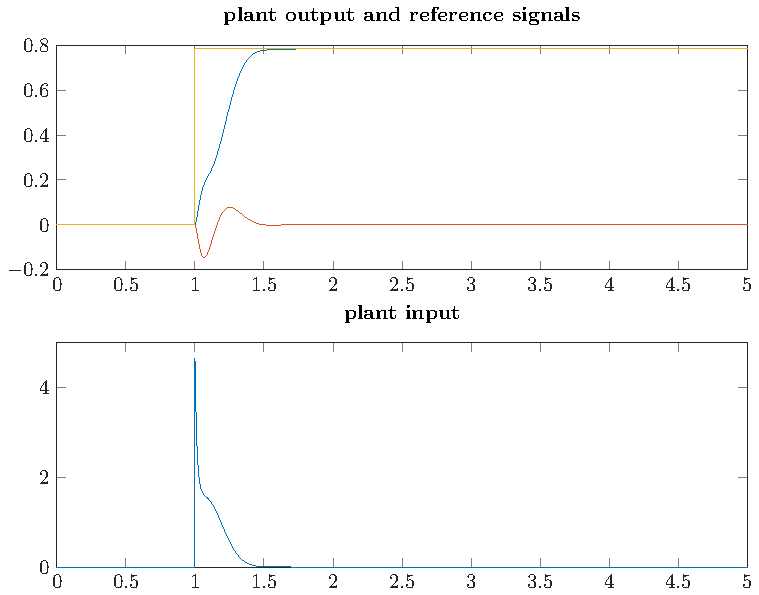
\includegraphics[scale=0.46]{images/orgFullState.pdf}
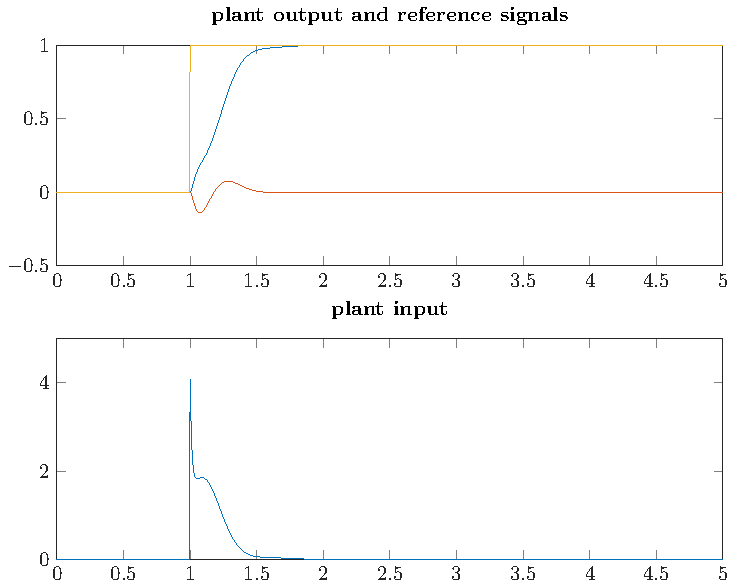
\includegraphics[scale=0.46]{images/optFullState.pdf}
\caption{Simulation results for the original weighting parameters left and for the improved weighting parameters right. Plant input is given in Volt [V]. Plant output and references are given in radians [rad].}
\label{fig:stepResponse}
\end{figure}


\section{Concluding Simulations with filter and differentiator}
\begin{figure}
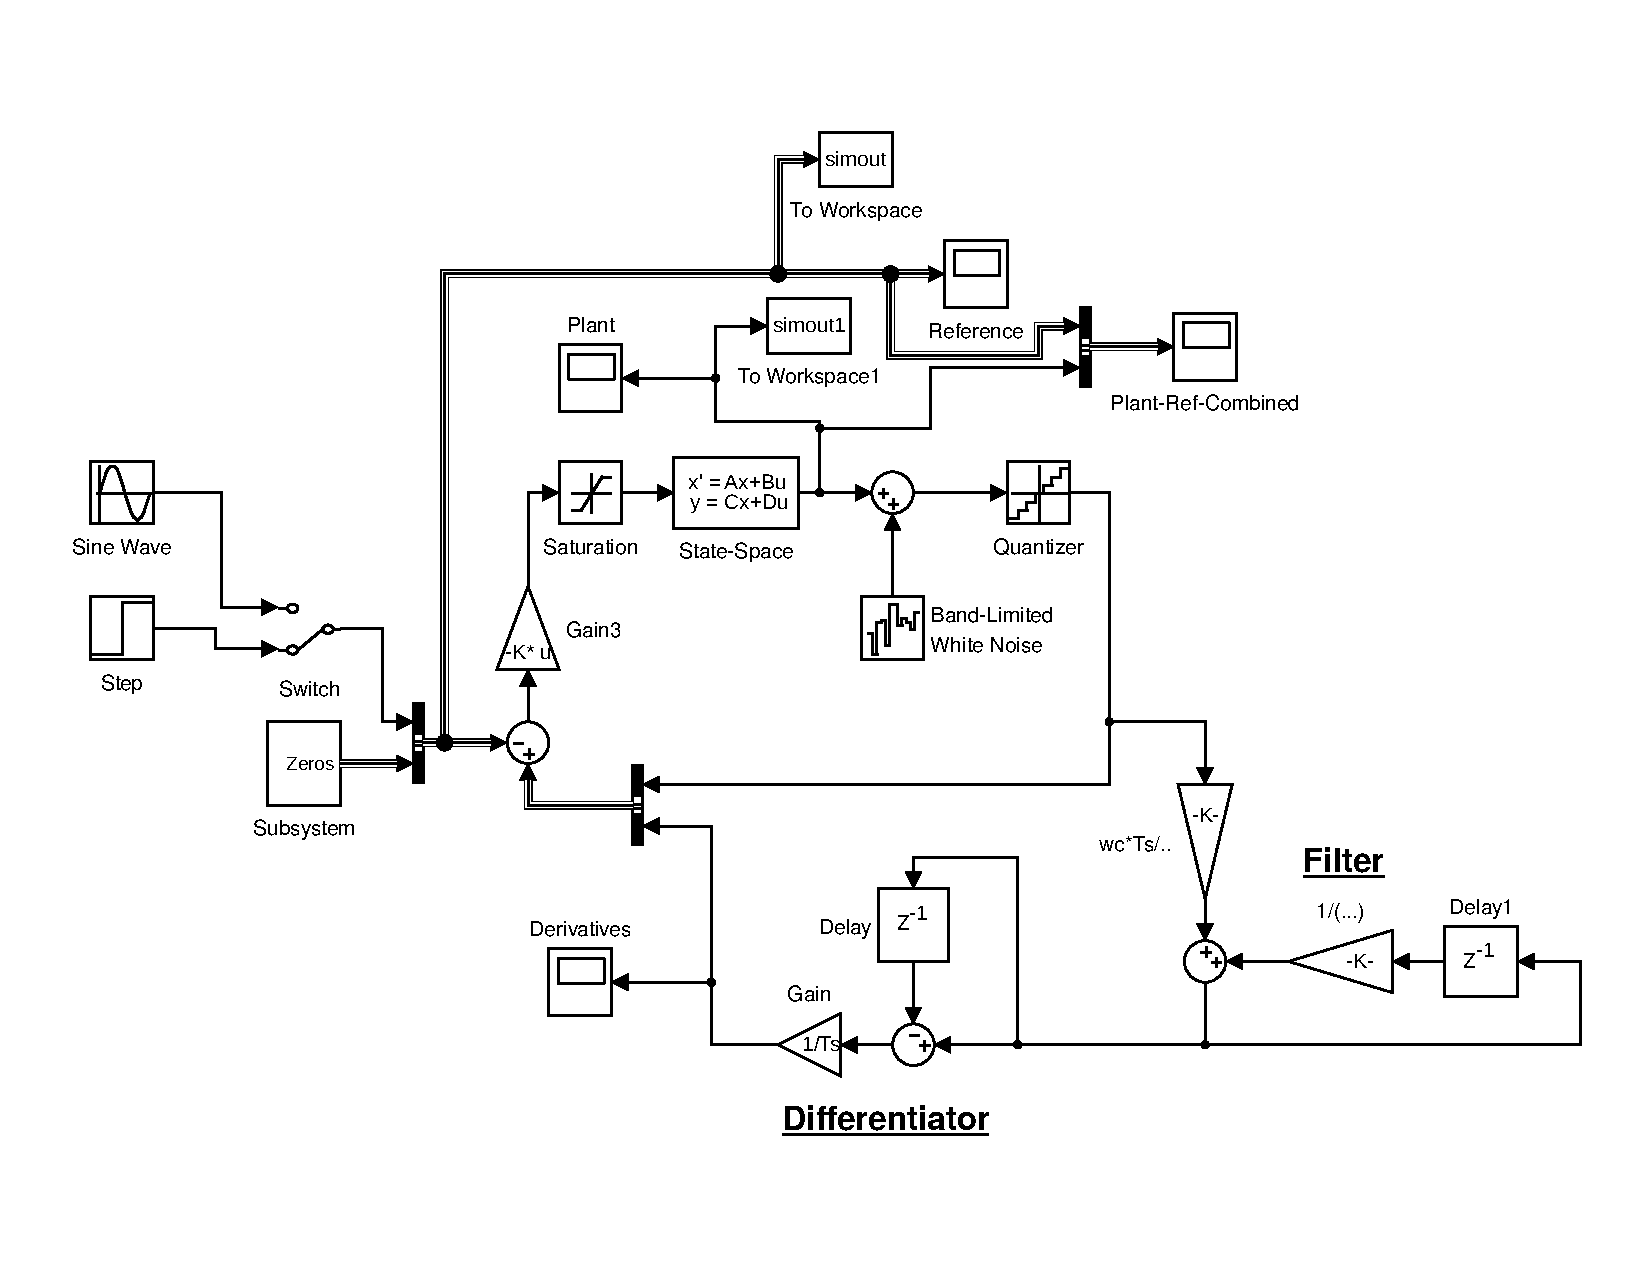
\includegraphics[scale=0.5]{images/simModel.pdf}
\caption{The simulink Layout of our Simulation}
\end{figure}



\chapter{Tests of the controller on the real setup}

\begin{figure} \label{realtimeSimDiagram}
  \centering
  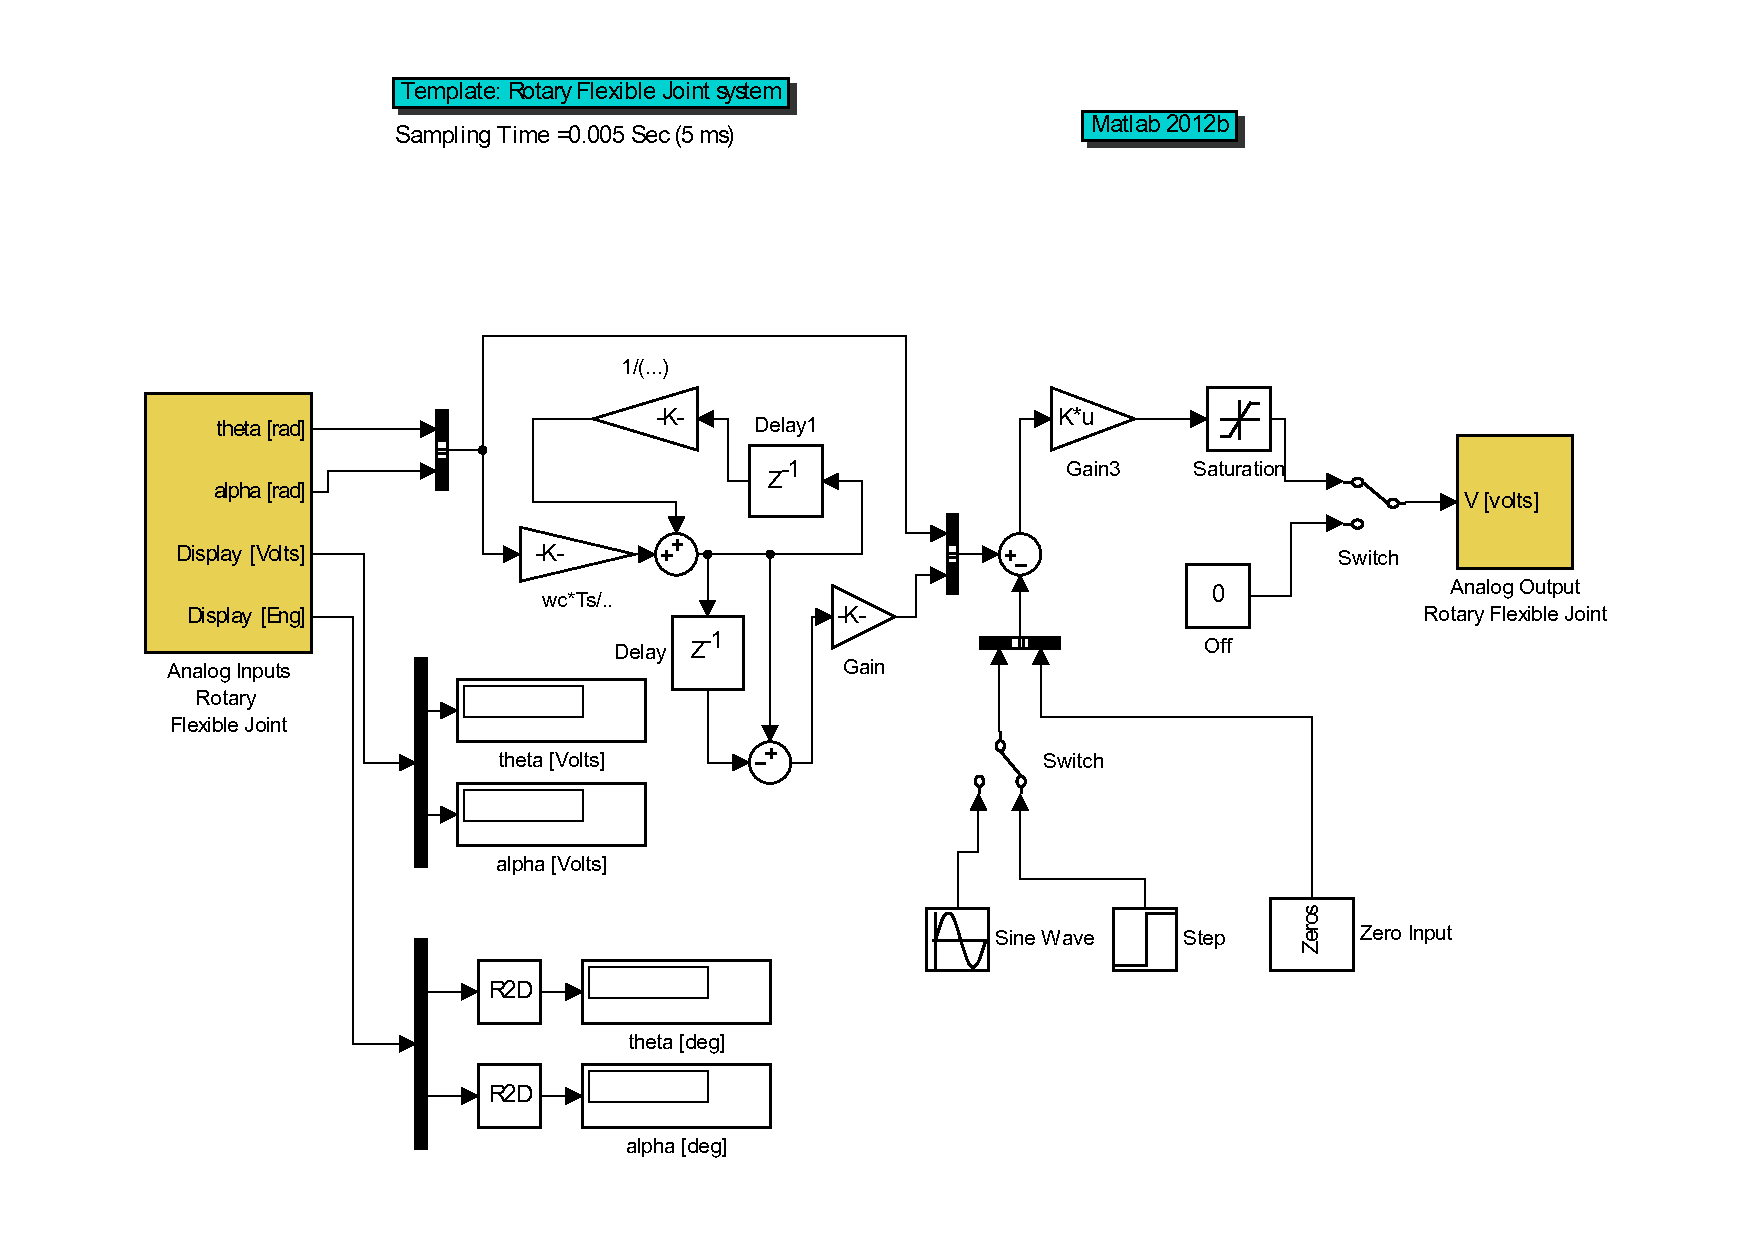
\includegraphics[scale=0.4]{images/realtimeSimDiagram}
  \caption{Real-time Simulink diagram} 
\end{figure}

In figure $\eqref{realtimeSimDiagram}$ we see the real-time Simulink diagram that we used in the lab to run our experiments on the real setup. The "Analog Input" block sends measurements of the sensors into the template. Each sensor reading is updated with a sampling time of 5 ms, in radians for the angles of the hub and arm. Additionally this block has two special outputs, "Display[volts]" and "Display[Eng]", which are used for visualization purposes. These two outputs are connected to a set of displays in order to provide a local visual measure of the process variables. 

The "Analog Output" block allows the controller to send a voltage signal to the motor of the hub. At the input of this block there is an on-off switch. This switch allows the user to switch the motor on or off. We included a saturator in our diagram just before the signal goes in to the "Analog Output" to limit the control input within $-5V$ and $5V$. The saturation settings of the block in our diagram are set accordingly. We also included a sine wave, a step input and a zero input. These two block are used as a reference for $\theta_{desired}$. The zero block contains 3 signals equal to zero that represent the references for $\alpha, \dot{\theta}$ and $\dot{\alpha}$.


\section{Setpoint tracking}
\begin{figure}
%If time later use these and adjust size in .tex file.
%% This file was created by matlab2tikz v0.4.7 running on MATLAB 8.4.
% Copyright (c) 2008--2014, Nico Schlömer <nico.schloemer@gmail.com>
% All rights reserved.
% Minimal pgfplots version: 1.3
% 
% The latest updates can be retrieved from
%   http://www.mathworks.com/matlabcentral/fileexchange/22022-matlab2tikz
% where you can also make suggestions and rate matlab2tikz.
% 
\documentclass[tikz]{standalone}
\usepackage{pgfplots}
\usepackage{grffile}
\pgfplotsset{compat=newest}
\usetikzlibrary{plotmarks}
\usepackage{amsmath}

\begin{document}
%
% defining custom colors
\definecolor{mycolor1}{rgb}{0.00000,0.44700,0.74100}%
\definecolor{mycolor2}{rgb}{0.85000,0.32500,0.09800}%
\definecolor{mycolor3}{rgb}{0.92900,0.69400,0.12500}%
%
\begin{tikzpicture}

\begin{axis}[%
width=2in,
height=1in,
scale only axis,
separate axis lines,
every outer x axis line/.append style={white!15!black},
every x tick label/.append style={font=\color{white!15!black}},
xmin=0,
xmax=7,
xmajorgrids,
every outer y axis line/.append style={white!15!black},
every y tick label/.append style={font=\color{white!15!black}},
ymin=-20,
ymax=60,
ymajorgrids,
name=plot1,
title style={font=\bfseries},
ylabel={reference, plant [$\;^\circ$]}
]
\addplot [color=mycolor1,solid,forget plot]
  table[row sep=crcr]{0	-1.81449008178188\\
0.005	-1.75197319638422\\
0.01	-1.78323163908305\\
0.015	-1.84574852448072\\
0.02	-1.83532904358111\\
0.025	-1.75197319638422\\
0.03	-1.80407060088227\\
0.035	-1.84574852448072\\
0.04	-1.77281215818344\\
0.045	-1.68945631098655\\
0.05	-1.68945631098655\\
0.055	-1.77281215818344\\
0.06	-1.73113423458499\\
0.065	-1.64777838738811\\
0.07	-1.65819786828772\\
0.075	-1.74155371548461\\
0.08	-1.67903683008694\\
0.085	-1.54358357839199\\
0.09	-1.56442254019122\\
0.095	-1.65819786828772\\
0.1	-1.60610046378966\\
0.105	-1.50190565479355\\
0.11	-1.54358357839199\\
0.115	-1.60610046378966\\
0.12	-1.56442254019122\\
0.125	-1.43938876939588\\
0.13	-1.4602277311951\\
0.135	-1.52274461659277\\
0.14	-1.48106669299433\\
0.145	-1.40813032669705\\
0.15	-1.38729136489783\\
0.155	-1.48106669299433\\
0.16	-1.43938876939588\\
0.165	-1.3664524030986\\
0.17	-1.38729136489783\\
0.175	-1.48106669299433\\
0.18	-1.42896928849627\\
0.185	-1.34561344129938\\
0.19	-1.33519396039977\\
0.195	-1.42896928849627\\
0.2	-1.39771084579744\\
0.205	-1.31435499860055\\
0.21	-1.33519396039977\\
0.215	-1.43938876939588\\
0.22	-1.42896928849627\\
0.225	-1.33519396039977\\
0.23	-1.34561344129938\\
0.235	-1.42896928849627\\
0.24	-1.41854980759666\\
0.245	-1.30393551770094\\
0.25	-1.34561344129938\\
0.255	-1.42896928849627\\
0.26	-1.41854980759666\\
0.265	-1.33519396039977\\
0.27	-1.33519396039977\\
0.275	-1.43938876939588\\
0.28	-1.44980825029549\\
0.285	-1.30393551770094\\
0.29	-1.32477447950016\\
0.295	-1.42896928849627\\
0.3	-1.40813032669705\\
0.305	-1.32477447950016\\
0.31	-1.32477447950016\\
0.315	-1.42896928849627\\
0.32	-1.41854980759666\\
0.325	-1.31435499860055\\
0.33	-1.3664524030986\\
0.335	-1.39771084579744\\
0.34	-1.41854980759666\\
0.345	-1.29351603680133\\
0.35	-1.35603292219899\\
0.355	-1.42896928849627\\
0.36	-1.41854980759666\\
0.365	-1.32477447950016\\
0.37	-1.34561344129938\\
0.375	-1.43938876939588\\
0.38	-1.42896928849627\\
0.385	-1.33519396039977\\
0.39	-1.33519396039977\\
0.395	-1.41854980759666\\
0.4	-1.42896928849627\\
0.405	-1.32477447950016\\
0.41	-1.35603292219899\\
0.415	-1.43938876939588\\
0.42	-1.40813032669705\\
0.425	-1.32477447950016\\
0.43	-1.33519396039977\\
0.435	-1.42896928849627\\
0.44	-1.40813032669705\\
0.445	-1.31435499860055\\
0.45	-1.3664524030986\\
0.455	-1.43938876939588\\
0.46	-1.41854980759666\\
0.465	-1.32477447950016\\
0.47	-1.34561344129938\\
0.475	-1.43938876939588\\
0.48	-1.40813032669705\\
0.485	-1.31435499860055\\
0.49	-1.35603292219899\\
0.495	-1.42896928849627\\
0.5	-1.39771084579744\\
0.505	-1.30393551770094\\
0.51	-1.34561344129938\\
0.515	-1.42896928849627\\
0.52	-1.41854980759666\\
0.525	-1.34561344129938\\
0.53	-1.32477447950016\\
0.535	-1.44980825029549\\
0.54	-1.42896928849627\\
0.545	-1.32477447950016\\
0.55	-1.35603292219899\\
0.555	-1.42896928849627\\
0.56	-1.40813032669705\\
0.565	-1.32477447950016\\
0.57	-1.33519396039977\\
0.575	-1.44980825029549\\
0.58	-1.42896928849627\\
0.585	-1.33519396039977\\
0.59	-1.32477447950016\\
0.595	-1.42896928849627\\
0.6	-1.40813032669705\\
0.605	-1.32477447950016\\
0.61	-1.37687188399822\\
0.615	-1.42896928849627\\
0.62	-1.40813032669705\\
0.625	-1.31435499860055\\
0.63	-1.34561344129938\\
0.635	-1.44980825029549\\
0.64	-1.40813032669705\\
0.645	-1.31435499860055\\
0.65	-1.33519396039977\\
0.655	-1.41854980759666\\
0.66	-1.42896928849627\\
0.665	-1.30393551770094\\
0.67	-1.35603292219899\\
0.675	-1.43938876939588\\
0.68	-1.40813032669705\\
0.685	-1.32477447950016\\
0.69	-1.3664524030986\\
0.695	-1.42896928849627\\
0.7	-1.40813032669705\\
0.705	-1.33519396039977\\
0.71	-1.33519396039977\\
0.715	-1.41854980759666\\
0.72	-1.40813032669705\\
0.725	-1.32477447950016\\
0.73	-1.33519396039977\\
0.735	-1.41854980759666\\
0.74	-1.41854980759666\\
0.745	-1.31435499860055\\
0.75	-1.35603292219899\\
0.755	-1.42896928849627\\
0.76	-1.41854980759666\\
0.765	-1.30393551770094\\
0.77	-1.35603292219899\\
0.775	-1.41854980759666\\
0.78	-1.40813032669705\\
0.785	-1.30393551770094\\
0.79	-1.32477447950016\\
0.795	-1.42896928849627\\
0.8	-1.43938876939588\\
0.805	-1.32477447950016\\
0.81	-1.34561344129938\\
0.815	-1.43938876939588\\
0.82	-1.41854980759666\\
0.825	-1.31435499860055\\
0.83	-1.33519396039977\\
0.835	-1.41854980759666\\
0.84	-1.41854980759666\\
0.845	-1.32477447950016\\
0.85	-1.31435499860055\\
0.855	-1.39771084579744\\
0.86	-1.40813032669705\\
0.865	-1.33519396039977\\
0.87	-1.30393551770094\\
0.875	-1.43938876939588\\
0.88	-1.42896928849627\\
0.885	-1.33519396039977\\
0.89	-1.32477447950016\\
0.895	-1.41854980759666\\
0.9	-1.41854980759666\\
0.905	-1.33519396039977\\
0.91	-1.33519396039977\\
0.915	-1.40813032669705\\
0.92	-1.39771084579744\\
0.925	-1.31435499860055\\
0.93	-1.32477447950016\\
0.935	-1.42896928849627\\
0.94	-1.41854980759666\\
0.945	-1.33519396039977\\
0.95	-1.32477447950016\\
0.955	-1.40813032669705\\
0.96	-1.41854980759666\\
0.965	-1.31435499860055\\
0.97	-1.32477447950016\\
0.975	-1.42896928849627\\
0.98	-1.39771084579744\\
0.985	-1.31435499860055\\
0.99	-1.33519396039977\\
0.995	-1.41854980759666\\
1	-1.40813032669705\\
1.005	-1.91868489077799\\
1.01	-1.47064721209472\\
1.015	-0.86631731991727\\
1.02	-0.147373137844102\\
1.025	0.759121700422066\\
1.03	1.62393861508979\\
1.035	2.30120487356451\\
1.04	3.1347633455334\\
1.045	3.96832181750229\\
1.05	4.61432963327819\\
1.055	5.05194783106185\\
1.06	5.48956602884552\\
1.065	5.98970111202685\\
1.07	6.32312450081441\\
1.075	6.53151411880663\\
1.08	6.83367906489536\\
1.085	7.20878037728136\\
1.09	7.54220376606891\\
1.095	7.76101286496075\\
1.1	8.02149988745103\\
1.105	8.4695375661343\\
1.11	8.8446388785203\\
1.115	9.09470642011097\\
1.12	9.48022721339658\\
1.125	10.0428791819756\\
1.13	10.4492389370604\\
1.135	10.8764376539445\\
1.14	11.397411698925\\
1.145	12.0642584765001\\
1.15	12.7311052540753\\
1.155	13.2520792990558\\
1.16	13.9085065957313\\
1.165	14.6899676632022\\
1.17	15.3776534025765\\
1.175	16.0028222565531\\
1.18	16.7426054004255\\
1.185	17.5970028341937\\
1.19	18.336785978066\\
1.195	18.9619548320427\\
1.2	19.5767042051198\\
1.205	20.2852289062933\\
1.21	20.9312367220692\\
1.215	21.4209523243509\\
1.22	22.035701697428\\
1.225	22.7338069177019\\
1.23	23.3381368098794\\
1.235	23.8070134503619\\
1.24	24.3384069762421\\
1.245	24.9114784257207\\
1.25	25.4324524707012\\
1.255	25.8492317066857\\
1.26	26.3597862707666\\
1.265	26.9953746056429\\
1.27	27.5267681315231\\
1.275	27.9227084057083\\
1.28	28.3811655652912\\
1.285	28.9542370147698\\
1.29	29.3605967698546\\
1.295	29.7565370440398\\
1.3	30.1524773182251\\
1.305	30.6838708441052\\
1.31	31.0798111182905\\
1.315	31.36113710258\\
1.32	31.6841410104679\\
1.325	32.1946955745489\\
1.33	32.4656020779387\\
1.335	32.6635722150314\\
1.34	32.9240592375216\\
1.345	33.288741069008\\
1.35	33.5283891296991\\
1.355	33.6534229004944\\
1.36	33.9139099229847\\
1.365	34.226494349973\\
1.37	34.414045006166\\
1.375	34.5078203342625\\
1.38	34.6641125477567\\
1.385	34.9662774938454\\
1.39	35.1746671118376\\
1.395	35.2892814017334\\
1.4	35.4768320579264\\
1.405	35.7789970040151\\
1.41	35.9457086984089\\
1.415	36.0082255838065\\
1.42	36.1436788355015\\
1.425	36.4041658579917\\
1.43	36.5291996287871\\
1.435	36.5396191096867\\
1.44	36.6854918422813\\
1.445	36.852203536675\\
1.45	36.9668178265707\\
1.455	36.9668178265707\\
1.46	37.0501736737676\\
1.465	37.2377243299606\\
1.47	37.2481438108602\\
1.475	37.2064658872618\\
1.48	37.2377243299606\\
1.485	37.3314996580571\\
1.49	37.3940165434548\\
1.495	37.3314996580571\\
1.5	37.4044360243544\\
1.505	37.5294697951498\\
1.51	37.5919866805474\\
1.515	37.550308756949\\
1.52	37.5919866805474\\
1.525	37.7586983749412\\
1.53	37.8107957794393\\
1.535	37.737859413142\\
1.54	37.8003762985396\\
1.545	37.9358295502346\\
1.55	37.9670879929334\\
1.555	37.9045711075357\\
1.56	37.9149905884354\\
1.565	38.0296048783311\\
1.57	38.0712828019295\\
1.575	37.977507473833\\
1.58	38.0296048783311\\
1.585	38.1442191682268\\
1.59	38.1963165727249\\
1.595	38.1546386491264\\
1.6	38.1858970918252\\
1.605	38.300511381721\\
1.61	38.352608786219\\
1.615	38.300511381721\\
1.62	38.352608786219\\
1.625	38.5089009997132\\
1.63	38.5714178851109\\
1.635	38.5089009997132\\
1.64	38.5297399615124\\
1.645	38.6860321750066\\
1.65	38.727710098605\\
1.655	38.6339347705085\\
1.66	38.6964516559062\\
1.665	38.8527438694004\\
1.67	38.9360997165973\\
1.675	38.8840023120992\\
1.68	38.9256802356976\\
1.685	39.0715529682922\\
1.69	39.1340698536899\\
1.695	39.0819724491918\\
1.7	39.1132308918906\\
1.705	39.2486841435856\\
1.71	39.3320399907825\\
1.715	39.2695231053848\\
1.72	39.3007815480836\\
1.725	39.4674932424774\\
1.73	39.5091711660759\\
1.735	39.4674932424774\\
1.74	39.4987516851763\\
1.745	39.6446244177708\\
1.75	39.6758828604696\\
1.755	39.6550438986704\\
1.76	39.6758828604696\\
1.765	39.8321750739638\\
1.77	39.8634335166626\\
1.775	39.8217555930642\\
1.78	39.8217555930642\\
1.785	39.9676283256588\\
1.79	40.0509841728556\\
1.795	39.9572088447591\\
1.8	39.9467893638595\\
1.805	40.0926620964541\\
1.81	40.1551789818518\\
1.815	40.040564691956\\
1.82	40.0509841728556\\
1.825	40.1864374245506\\
1.83	40.2385348290486\\
1.835	40.1655984627514\\
1.84	40.176017943651\\
1.845	40.3010517144463\\
1.85	40.3218906762455\\
1.855	40.2489543099483\\
1.86	40.228115348149\\
1.865	40.3948270425428\\
1.87	40.4573439279405\\
1.875	40.3531491189444\\
1.88	40.3531491189444\\
1.885	40.4886023706393\\
1.89	40.5302802942378\\
1.895	40.4573439279405\\
1.9	40.4677634088401\\
1.905	40.6136361414346\\
1.91	40.6240556223343\\
1.915	40.5615387369366\\
1.92	40.551119256037\\
1.925	40.6657335459327\\
1.93	40.6969919886315\\
1.935	40.6136361414346\\
1.94	40.6344751032339\\
1.945	40.7595088740292\\
1.95	40.8011867976276\\
1.955	40.6969919886315\\
1.96	40.7074114695311\\
1.965	40.8220257594269\\
1.97	40.8741231639249\\
1.975	40.790767316728\\
1.98	40.8116062785273\\
1.985	40.926220568423\\
1.99	40.9470595302222\\
1.995	40.8949621257241\\
2	40.9158010875234\\
2.005	40.9991569347203\\
2.01	41.0616738201179\\
2.015	40.978317972921\\
2.02	40.9678984920214\\
2.025	41.0929322628168\\
2.03	41.1241907055156\\
2.035	41.0095764156199\\
2.04	41.0304153774191\\
2.045	41.165868629114\\
2.05	41.1971270718129\\
2.055	41.1033517437164\\
2.06	41.0929322628168\\
2.065	41.2283855145117\\
2.07	41.2804829190098\\
2.075	41.1867075909133\\
2.08	41.1554491482144\\
2.085	41.301321880809\\
2.09	41.3429998044074\\
2.095	41.2388049954113\\
2.1	41.2492244763109\\
2.105	41.353419285307\\
2.11	41.353419285307\\
2.115	41.2909023999094\\
2.12	41.2700634381101\\
2.125	41.3846777280059\\
2.13	41.4159361707047\\
2.135	41.3117413617086\\
2.14	41.3117413617086\\
2.145	41.4159361707047\\
2.15	41.4680335752028\\
2.155	41.3742582471063\\
2.16	41.3429998044074\\
2.165	41.4576140943031\\
2.17	41.5305504606004\\
2.175	41.4055166898051\\
2.18	41.3950972089055\\
2.185	41.5201309797008\\
2.19	41.5513894223996\\
2.195	41.4576140943031\\
2.2	41.4055166898051\\
2.205	41.5409699415\\
2.21	41.5722283841989\\
2.215	41.4784530561024\\
2.22	41.4471946134035\\
2.225	41.5826478650985\\
2.23	41.6139063077973\\
2.235	41.5097114988012\\
2.24	41.488872537002\\
2.245	41.5930673459981\\
2.25	41.6347452695965\\
2.255	41.4992920179016\\
2.26	41.4784530561024\\
2.265	41.5722283841989\\
2.27	41.6034868268977\\
2.275	41.5097114988012\\
2.28	41.4784530561024\\
2.285	41.5722283841989\\
2.29	41.5930673459981\\
2.295	41.5305504606004\\
2.3	41.488872537002\\
2.305	41.6139063077973\\
2.31	41.5930673459981\\
2.315	41.4992920179016\\
2.32	41.5097114988012\\
2.325	41.6347452695965\\
2.33	41.6451647504961\\
2.335	41.5513894223996\\
2.34	41.5305504606004\\
2.345	41.6451647504961\\
2.35	41.6868426740946\\
2.355	41.5826478650985\\
2.36	41.5305504606004\\
2.365	41.6451647504961\\
2.37	41.676423193195\\
2.375	41.5826478650985\\
2.38	41.5409699415\\
2.385	41.676423193195\\
2.39	41.6868426740946\\
2.395	41.6139063077973\\
2.4	41.5722283841989\\
2.405	41.6972621549942\\
2.41	41.7493595594923\\
2.415	41.6660037122954\\
2.42	41.6034868268977\\
2.425	41.7181011167934\\
2.43	41.7597790403919\\
2.435	41.6451647504961\\
2.44	41.6347452695965\\
2.445	41.7493595594923\\
2.45	41.7701985212915\\
2.455	41.6972621549942\\
2.46	41.676423193195\\
2.465	41.7806180021911\\
2.47	41.8327154066891\\
2.475	41.7181011167934\\
2.48	41.7181011167934\\
2.485	41.8014569639903\\
2.49	41.8535543684884\\
2.495	41.7806180021911\\
2.5	41.7389400785926\\
2.505	41.8431348875888\\
2.51	41.863973849388\\
2.515	41.7806180021911\\
2.52	41.7181011167934\\
2.525	41.863973849388\\
2.53	41.8848128111872\\
2.535	41.7910374830907\\
2.54	41.7701985212915\\
2.545	41.8743933302876\\
2.55	41.9369102156853\\
2.555	41.8014569639903\\
2.56	41.7910374830907\\
2.565	41.863973849388\\
2.57	41.9369102156853\\
2.575	41.8222959257895\\
2.58	41.8014569639903\\
2.585	41.9264907347857\\
2.59	41.9473296965849\\
2.595	41.8535543684884\\
2.6	41.7806180021911\\
2.605	41.8952322920868\\
2.61	41.9369102156853\\
2.615	41.8327154066891\\
2.62	41.8327154066891\\
2.625	41.9369102156853\\
2.63	41.9890076201833\\
2.635	41.8431348875888\\
2.64	41.8222959257895\\
2.645	41.9681686583841\\
2.65	41.9785881392837\\
2.655	41.8535543684884\\
2.66	41.8014569639903\\
2.665	41.9056517729864\\
2.67	41.9577491774845\\
2.675	41.8535543684884\\
2.68	41.8014569639903\\
2.685	41.9056517729864\\
2.69	41.9681686583841\\
2.695	41.8535543684884\\
2.7	41.8014569639903\\
2.705	41.9264907347857\\
2.71	41.9473296965849\\
2.715	41.8535543684884\\
2.72	41.8118764448899\\
2.725	41.9369102156853\\
2.73	41.9785881392837\\
2.735	41.8848128111872\\
2.74	41.8222959257895\\
2.745	41.9264907347857\\
2.75	41.9890076201833\\
2.755	41.8743933302876\\
2.76	41.8431348875888\\
2.765	41.9473296965849\\
2.77	41.9785881392837\\
2.775	41.8848128111872\\
2.78	41.8327154066891\\
2.785	41.9473296965849\\
2.79	41.9577491774845\\
2.795	41.8743933302876\\
2.8	41.8327154066891\\
2.805	41.9473296965849\\
2.81	41.9890076201833\\
2.815	41.8848128111872\\
2.82	41.8535543684884\\
2.825	41.9681686583841\\
2.83	42.0098465819825\\
2.835	41.8952322920868\\
2.84	41.8743933302876\\
2.845	41.9473296965849\\
2.85	41.9890076201833\\
2.855	41.8952322920868\\
2.86	41.863973849388\\
2.865	41.9577491774845\\
2.87	42.0098465819825\\
2.875	41.916071253886\\
2.88	41.8743933302876\\
2.885	41.9785881392837\\
2.89	42.0098465819825\\
2.895	41.916071253886\\
2.9	41.863973849388\\
2.905	41.9577491774845\\
2.91	42.0202660628821\\
2.915	41.9369102156853\\
2.92	41.8952322920868\\
2.925	41.9994271010829\\
2.93	42.0619439864806\\
2.935	41.9369102156853\\
2.94	41.8743933302876\\
2.945	41.9785881392837\\
2.95	42.0411050246814\\
2.955	41.9473296965849\\
2.96	41.8848128111872\\
2.965	41.9785881392837\\
2.97	42.0306855437818\\
2.975	41.9369102156853\\
2.98	41.8743933302876\\
2.985	42.0098465819825\\
2.99	42.051524505581\\
2.995	41.9369102156853\\
3	41.916071253886\\
3.005	41.9994271010829\\
3.01	42.0619439864806\\
3.015	41.9577491774845\\
3.02	41.9264907347857\\
3.025	42.0098465819825\\
3.03	42.0619439864806\\
3.035	41.9681686583841\\
3.04	41.916071253886\\
3.045	42.0619439864806\\
3.05	42.0723634673802\\
3.055	41.9890076201833\\
3.06	41.9264907347857\\
3.065	42.0098465819825\\
3.07	42.051524505581\\
3.075	41.9785881392837\\
3.08	41.9369102156853\\
3.085	42.0202660628821\\
3.09	42.0827829482798\\
3.095	41.9890076201833\\
3.1	41.9577491774845\\
3.105	42.0619439864806\\
3.11	42.0827829482798\\
3.115	41.9785881392837\\
3.12	41.9473296965849\\
3.125	42.0411050246814\\
3.13	42.0827829482798\\
3.135	42.0306855437818\\
3.14	41.9473296965849\\
3.145	42.0619439864806\\
3.15	42.1244608718783\\
3.155	42.0098465819825\\
3.16	41.9681686583841\\
3.165	42.0827829482798\\
3.17	42.1244608718783\\
3.175	41.9994271010829\\
3.18	41.9994271010829\\
3.185	42.0827829482798\\
3.19	42.1348803527779\\
3.195	42.0306855437818\\
3.2	41.9681686583841\\
3.205	42.0827829482798\\
3.21	42.1244608718783\\
3.215	42.0098465819825\\
3.22	41.9890076201833\\
3.225	42.103621910079\\
3.23	42.1557193145771\\
3.235	42.0098465819825\\
3.24	41.9890076201833\\
3.245	42.0723634673802\\
3.25	42.1348803527779\\
3.255	42.051524505581\\
3.26	42.0098465819825\\
3.265	42.1140413909786\\
3.27	42.1557193145771\\
3.275	42.0619439864806\\
3.28	42.0202660628821\\
3.285	42.0827829482798\\
3.29	42.1452998336775\\
3.295	42.0723634673802\\
3.3	41.9890076201833\\
3.305	42.0932024291794\\
3.31	42.1348803527779\\
3.315	42.0723634673802\\
3.32	42.0098465819825\\
3.325	42.1140413909786\\
3.33	42.1869777572759\\
3.335	42.0932024291794\\
3.34	42.0411050246814\\
3.345	42.1244608718783\\
3.35	42.1869777572759\\
3.355	42.0932024291794\\
3.36	42.0306855437818\\
3.365	42.1244608718783\\
3.37	42.1661387954767\\
3.375	42.0723634673802\\
3.38	42.051524505581\\
3.385	42.1244608718783\\
3.39	42.1973972381755\\
3.395	42.0619439864806\\
3.4	42.0306855437818\\
3.405	42.1452998336775\\
3.41	42.2078167190751\\
3.415	42.1140413909786\\
3.42	42.051524505581\\
3.425	42.1452998336775\\
3.43	42.2182361999748\\
3.435	42.1140413909786\\
3.44	42.0411050246814\\
3.445	42.1557193145771\\
3.45	42.2182361999748\\
3.455	42.103621910079\\
3.46	42.0306855437818\\
3.465	42.1557193145771\\
3.47	42.2078167190751\\
3.475	42.1140413909786\\
3.48	42.0827829482798\\
3.485	42.1557193145771\\
3.49	42.2078167190751\\
3.495	42.1348803527779\\
3.5	42.051524505581\\
3.505	42.1765582763763\\
3.51	42.2078167190751\\
3.515	42.1348803527779\\
3.52	42.0619439864806\\
3.525	42.1869777572759\\
3.53	42.239075161774\\
3.535	42.1244608718783\\
3.54	42.0619439864806\\
3.545	42.1765582763763\\
3.55	42.2286556808744\\
3.555	42.1661387954767\\
3.56	42.0827829482798\\
3.565	42.1765582763763\\
3.57	42.2494946426736\\
3.575	42.1661387954767\\
3.58	42.0827829482798\\
3.585	42.1869777572759\\
3.59	42.2494946426736\\
3.595	42.1557193145771\\
3.6	42.0827829482798\\
3.605	42.1869777572759\\
3.61	42.2703336044728\\
3.615	42.1765582763763\\
3.62	42.0619439864806\\
3.625	42.2286556808744\\
3.63	42.2703336044728\\
3.635	42.1452998336775\\
3.64	42.0932024291794\\
3.645	42.1869777572759\\
3.65	42.2494946426736\\
3.655	42.1557193145771\\
3.66	42.0827829482798\\
3.665	42.2182361999748\\
3.67	42.239075161774\\
3.675	42.1452998336775\\
3.68	42.1140413909786\\
3.685	42.2182361999748\\
3.69	42.2703336044728\\
3.695	42.1765582763763\\
3.7	42.0932024291794\\
3.705	42.1869777572759\\
3.71	42.2286556808744\\
3.715	42.1557193145771\\
3.72	42.0932024291794\\
3.725	42.2286556808744\\
3.73	42.2807530853724\\
3.735	42.1661387954767\\
3.74	42.1140413909786\\
3.745	42.2286556808744\\
3.75	42.2703336044728\\
3.755	42.1557193145771\\
3.76	42.103621910079\\
3.765	42.2286556808744\\
3.77	42.3015920471716\\
3.775	42.1348803527779\\
3.78	42.1244608718783\\
3.785	42.2182361999748\\
3.79	42.3015920471716\\
3.795	42.1869777572759\\
3.8	42.1140413909786\\
3.805	42.2286556808744\\
3.81	42.3015920471716\\
3.815	42.1973972381755\\
3.82	42.1348803527779\\
3.825	42.2182361999748\\
3.83	42.291172566272\\
3.835	42.1869777572759\\
3.84	42.1140413909786\\
3.845	42.2286556808744\\
3.85	42.3120115280713\\
3.855	42.1869777572759\\
3.86	42.1244608718783\\
3.865	42.2286556808744\\
3.87	42.3120115280713\\
3.875	42.1869777572759\\
3.88	42.1140413909786\\
3.885	42.2494946426736\\
3.89	42.3015920471716\\
3.895	42.1765582763763\\
3.9	42.1140413909786\\
3.905	42.2494946426736\\
3.91	42.291172566272\\
3.915	42.2078167190751\\
3.92	42.1348803527779\\
3.925	42.2286556808744\\
3.93	42.2807530853724\\
3.935	42.1869777572759\\
3.94	42.1348803527779\\
3.945	42.2182361999748\\
3.95	42.3120115280713\\
3.955	42.1973972381755\\
3.96	42.1244608718783\\
3.965	42.239075161774\\
3.97	42.3015920471716\\
3.975	42.1869777572759\\
3.98	42.1452998336775\\
3.985	42.2494946426736\\
3.99	42.291172566272\\
3.995	42.1765582763763\\
4	42.1244608718783\\
4.005	42.2182361999748\\
4.01	42.3015920471716\\
4.015	42.1869777572759\\
4.02	42.1140413909786\\
4.025	42.2494946426736\\
4.03	42.3120115280713\\
4.035	42.1973972381755\\
4.04	42.1244608718783\\
4.045	42.2286556808744\\
4.05	42.3120115280713\\
4.055	42.1869777572759\\
4.06	42.1348803527779\\
4.065	42.239075161774\\
4.07	42.3328504898705\\
4.075	42.2078167190751\\
4.08	42.1348803527779\\
4.085	42.2703336044728\\
4.09	42.3224310089709\\
4.095	42.1973972381755\\
4.1	42.1557193145771\\
4.105	42.2286556808744\\
4.11	42.3328504898705\\
4.115	42.2182361999748\\
4.12	42.1244608718783\\
4.125	42.2494946426736\\
4.13	42.3120115280713\\
4.135	42.2182361999748\\
4.14	42.1557193145771\\
4.145	42.2599141235732\\
4.15	42.3120115280713\\
4.155	42.2286556808744\\
4.16	42.1557193145771\\
4.165	42.2494946426736\\
4.17	42.3432699707701\\
4.175	42.1973972381755\\
4.18	42.1557193145771\\
4.185	42.239075161774\\
4.19	42.3432699707701\\
4.195	42.2078167190751\\
4.2	42.1244608718783\\
4.205	42.2494946426736\\
4.21	42.3328504898705\\
4.215	42.2182361999748\\
4.22	42.1348803527779\\
4.225	42.2807530853724\\
4.23	42.3015920471716\\
4.235	42.2182361999748\\
4.24	42.1452998336775\\
4.245	42.239075161774\\
4.25	42.3120115280713\\
4.255	42.1973972381755\\
4.26	42.1140413909786\\
4.265	42.2599141235732\\
4.27	42.3120115280713\\
4.275	42.2182361999748\\
4.28	42.1452998336775\\
4.285	42.239075161774\\
4.29	42.3120115280713\\
4.295	42.2182361999748\\
4.3	42.1452998336775\\
4.305	42.2599141235732\\
4.31	42.3120115280713\\
4.315	42.2078167190751\\
4.32	42.1452998336775\\
4.325	42.239075161774\\
4.33	42.3120115280713\\
4.335	42.2182361999748\\
4.34	42.1557193145771\\
4.345	42.2599141235732\\
4.35	42.3224310089709\\
4.355	42.2286556808744\\
4.36	42.1765582763763\\
4.365	42.2703336044728\\
4.37	42.3328504898705\\
4.375	42.2286556808744\\
4.38	42.1244608718783\\
4.385	42.2703336044728\\
4.39	42.3120115280713\\
4.395	42.2182361999748\\
4.4	42.1557193145771\\
4.405	42.2599141235732\\
4.41	42.3224310089709\\
4.415	42.2286556808744\\
4.42	42.1765582763763\\
4.425	42.2807530853724\\
4.43	42.3120115280713\\
4.435	42.2182361999748\\
4.44	42.1452998336775\\
4.445	42.2703336044728\\
4.45	42.3536894516697\\
4.455	42.239075161774\\
4.46	42.1869777572759\\
4.465	42.2703336044728\\
4.47	42.3432699707701\\
4.475	42.2286556808744\\
4.48	42.1348803527779\\
4.485	42.2703336044728\\
4.49	42.3328504898705\\
4.495	42.239075161774\\
4.5	42.1557193145771\\
4.505	42.2807530853724\\
4.51	42.3432699707701\\
4.515	42.2182361999748\\
4.52	42.1765582763763\\
4.525	42.2807530853724\\
4.53	42.3328504898705\\
4.535	42.2286556808744\\
4.54	42.1765582763763\\
4.545	42.291172566272\\
4.55	42.3641089325693\\
4.555	42.2286556808744\\
4.56	42.1765582763763\\
4.565	42.3015920471716\\
4.57	42.3224310089709\\
4.575	42.239075161774\\
4.58	42.1557193145771\\
4.585	42.2703336044728\\
4.59	42.3432699707701\\
4.595	42.239075161774\\
4.6	42.1765582763763\\
4.605	42.2599141235732\\
4.61	42.3432699707701\\
4.615	42.2182361999748\\
4.62	42.1557193145771\\
4.625	42.2599141235732\\
4.63	42.3120115280713\\
4.635	42.2286556808744\\
4.64	42.1765582763763\\
4.645	42.2807530853724\\
4.65	42.3432699707701\\
4.655	42.2494946426736\\
4.66	42.1765582763763\\
4.665	42.2807530853724\\
4.67	42.3641089325693\\
4.675	42.2286556808744\\
4.68	42.1557193145771\\
4.685	42.291172566272\\
4.69	42.3536894516697\\
4.695	42.2599141235732\\
4.7	42.1765582763763\\
4.705	42.3015920471716\\
4.71	42.3328504898705\\
4.715	42.2494946426736\\
4.72	42.1869777572759\\
4.725	42.2703336044728\\
4.73	42.3536894516697\\
4.735	42.239075161774\\
4.74	42.1661387954767\\
4.745	42.2807530853724\\
4.75	42.3641089325693\\
4.755	42.239075161774\\
4.76	42.1557193145771\\
4.765	42.2807530853724\\
4.77	42.3745284134689\\
4.775	42.239075161774\\
4.78	42.1557193145771\\
4.785	42.2599141235732\\
4.79	42.3224310089709\\
4.795	42.2286556808744\\
4.8	42.1765582763763\\
4.805	42.291172566272\\
4.81	42.3328504898705\\
4.815	42.2599141235732\\
4.82	42.1765582763763\\
4.825	42.2807530853724\\
4.83	42.3536894516697\\
4.835	42.2494946426736\\
4.84	42.1973972381755\\
4.845	42.2703336044728\\
4.85	42.3641089325693\\
4.855	42.2599141235732\\
4.86	42.1661387954767\\
4.865	42.3120115280713\\
4.87	42.3536894516697\\
4.875	42.239075161774\\
4.88	42.1661387954767\\
4.885	42.2703336044728\\
4.89	42.3536894516697\\
4.895	42.2494946426736\\
4.9	42.1765582763763\\
4.905	42.3120115280713\\
4.91	42.3745284134689\\
4.915	42.2703336044728\\
4.92	42.1869777572759\\
4.925	42.3015920471716\\
4.93	42.3849478943685\\
4.935	42.239075161774\\
4.94	42.1661387954767\\
4.945	42.291172566272\\
4.95	42.3432699707701\\
4.955	42.2494946426736\\
4.96	42.1765582763763\\
4.965	42.3015920471716\\
4.97	42.3432699707701\\
4.975	42.239075161774\\
4.98	42.1765582763763\\
4.985	42.3224310089709\\
4.99	42.3432699707701\\
4.995	42.2599141235732\\
5	42.1869777572759\\
5.005	42.3015920471716\\
5.01	42.3745284134689\\
5.015	42.2599141235732\\
5.02	42.1973972381755\\
5.025	42.291172566272\\
5.03	42.3641089325693\\
5.035	42.239075161774\\
5.04	42.1869777572759\\
5.045	42.3224310089709\\
5.05	42.3745284134689\\
5.055	42.2807530853724\\
5.06	42.1869777572759\\
5.065	42.3015920471716\\
5.07	42.3745284134689\\
5.075	42.2703336044728\\
5.08	42.2182361999748\\
5.085	42.3120115280713\\
5.09	42.3745284134689\\
5.095	42.2599141235732\\
5.1	42.1765582763763\\
5.105	42.3328504898705\\
5.11	42.3641089325693\\
5.115	42.2599141235732\\
5.12	42.1869777572759\\
5.125	42.291172566272\\
5.13	42.3849478943685\\
5.135	42.2807530853724\\
5.14	42.2182361999748\\
5.145	42.3224310089709\\
5.15	42.3849478943685\\
5.155	42.2807530853724\\
5.16	42.2078167190751\\
5.165	42.3015920471716\\
5.17	42.3849478943685\\
5.175	42.291172566272\\
5.18	42.1973972381755\\
5.185	42.3015920471716\\
5.19	42.3641089325693\\
5.195	42.3015920471716\\
5.2	42.1869777572759\\
5.205	42.3224310089709\\
5.21	42.3641089325693\\
5.215	42.2807530853724\\
5.22	42.2078167190751\\
5.225	42.3328504898705\\
5.23	42.3849478943685\\
5.235	42.291172566272\\
5.24	42.2182361999748\\
5.245	42.3328504898705\\
5.25	42.3953673752682\\
5.255	42.2807530853724\\
5.26	42.2286556808744\\
5.265	42.3536894516697\\
5.27	42.3953673752682\\
5.275	42.3224310089709\\
5.28	42.239075161774\\
5.285	42.3536894516697\\
5.29	42.4057868561678\\
5.295	42.2807530853724\\
5.3	42.2286556808744\\
5.305	42.3536894516697\\
5.31	42.4057868561678\\
5.315	42.2807530853724\\
5.32	42.2286556808744\\
5.325	42.3536894516697\\
5.33	42.4162063370674\\
5.335	42.3120115280713\\
5.34	42.2599141235732\\
5.345	42.3328504898705\\
5.35	42.426625817967\\
5.355	42.3120115280713\\
5.36	42.2286556808744\\
5.365	42.3328504898705\\
5.37	42.4057868561678\\
5.375	42.3328504898705\\
5.38	42.239075161774\\
5.385	42.3224310089709\\
5.39	42.4370452988666\\
5.395	42.3224310089709\\
5.4	42.239075161774\\
5.405	42.3536894516697\\
5.41	42.4162063370674\\
5.415	42.3224310089709\\
5.42	42.239075161774\\
5.425	42.3328504898705\\
5.43	42.4057868561678\\
5.435	42.3224310089709\\
5.44	42.2494946426736\\
5.445	42.3641089325693\\
5.45	42.426625817967\\
5.455	42.3328504898705\\
5.46	42.2599141235732\\
5.465	42.3536894516697\\
5.47	42.4057868561678\\
5.475	42.3120115280713\\
5.48	42.2494946426736\\
5.485	42.3849478943685\\
5.49	42.4370452988666\\
5.495	42.3224310089709\\
5.5	42.239075161774\\
5.505	42.3536894516697\\
5.51	42.426625817967\\
5.515	42.3120115280713\\
5.52	42.2703336044728\\
5.525	42.3432699707701\\
5.53	42.426625817967\\
5.535	42.3120115280713\\
5.54	42.2599141235732\\
5.545	42.3432699707701\\
5.55	42.4370452988666\\
5.555	42.3432699707701\\
5.56	42.2807530853724\\
5.565	42.3641089325693\\
5.57	42.4474647797662\\
5.575	42.3120115280713\\
5.58	42.2807530853724\\
5.585	42.3953673752682\\
5.59	42.4683037415654\\
5.595	42.3432699707701\\
5.6	42.2807530853724\\
5.605	42.3849478943685\\
5.61	42.4578842606658\\
5.615	42.3641089325693\\
5.62	42.291172566272\\
5.625	42.3641089325693\\
5.63	42.4162063370674\\
5.635	42.3641089325693\\
5.64	42.3015920471716\\
5.645	42.4057868561678\\
5.65	42.4474647797662\\
5.655	42.3536894516697\\
5.66	42.2599141235732\\
5.665	42.3953673752682\\
5.67	42.4578842606658\\
5.675	42.3536894516697\\
5.68	42.2703336044728\\
5.685	42.3849478943685\\
5.69	42.4474647797662\\
5.695	42.3745284134689\\
5.7	42.3120115280713\\
5.705	42.3641089325693\\
5.71	42.4578842606658\\
5.715	42.3432699707701\\
5.72	42.291172566272\\
5.725	42.3849478943685\\
5.73	42.4474647797662\\
5.735	42.3536894516697\\
5.74	42.2807530853724\\
5.745	42.3953673752682\\
5.75	42.4578842606658\\
5.755	42.3641089325693\\
5.76	42.3120115280713\\
5.765	42.3849478943685\\
5.77	42.4474647797662\\
5.775	42.3536894516697\\
5.78	42.291172566272\\
5.785	42.3849478943685\\
5.79	42.4474647797662\\
5.795	42.3641089325693\\
5.8	42.291172566272\\
5.805	42.4162063370674\\
5.81	42.4683037415654\\
5.815	42.3536894516697\\
5.82	42.3015920471716\\
5.825	42.3849478943685\\
5.83	42.4683037415654\\
5.835	42.3745284134689\\
5.84	42.3015920471716\\
5.845	42.4162063370674\\
5.85	42.4891427033646\\
5.855	42.3849478943685\\
5.86	42.3224310089709\\
5.865	42.426625817967\\
5.87	42.478723222465\\
5.875	42.3641089325693\\
5.88	42.3015920471716\\
5.885	42.4162063370674\\
5.89	42.4578842606658\\
5.895	42.3849478943685\\
5.9	42.3015920471716\\
5.905	42.426625817967\\
5.91	42.4891427033646\\
5.915	42.3745284134689\\
5.92	42.3120115280713\\
5.925	42.4162063370674\\
5.93	42.4995621842643\\
5.935	42.4057868561678\\
5.94	42.3432699707701\\
5.945	42.4474647797662\\
5.95	42.4891427033646\\
5.955	42.3953673752682\\
5.96	42.3328504898705\\
5.965	42.4474647797662\\
5.97	42.478723222465\\
5.975	42.3849478943685\\
5.98	42.3224310089709\\
5.985	42.426625817967\\
5.99	42.4683037415654\\
5.995	42.3953673752682\\
6	42.3432699707701\\
6.005	42.4370452988666\\
6.01	42.4891427033646\\
6.015	42.3849478943685\\
6.02	42.3328504898705\\
6.025	42.4057868561678\\
6.03	42.4995621842643\\
6.035	42.4057868561678\\
6.04	42.3432699707701\\
6.045	42.4162063370674\\
6.05	42.4891427033646\\
6.055	42.4057868561678\\
6.06	42.3641089325693\\
6.065	42.4474647797662\\
6.07	42.4683037415654\\
6.075	42.3745284134689\\
6.08	42.3536894516697\\
6.085	42.4162063370674\\
6.09	42.4683037415654\\
6.095	42.4162063370674\\
6.1	42.3328504898705\\
6.105	42.4162063370674\\
6.11	42.4891427033646\\
6.115	42.4057868561678\\
};
\addplot [color=mycolor2,solid,forget plot]
  table[row sep=crcr]{0	0.121897638184183\\
0.005	0.16529611375531\\
0.01	0.147936723526859\\
0.015	0.100198400398619\\
0.02	0.11755779062707\\
0.025	0.16529611375531\\
0.03	0.147936723526859\\
0.035	0.00906160169925145\\
0.04	0.000381906585025969\\
0.045	0.0437803821561534\\
0.05	0.0394405345990406\\
0.055	0.0307608394848152\\
0.06	0.126237485741295\\
0.065	0.21303443688355\\
0.07	0.204354741769325\\
0.075	0.152276571083972\\
0.08	0.178315656426648\\
0.085	0.217374284440663\\
0.09	0.204354741769325\\
0.095	0.143596875969746\\
0.1	0.182655503983761\\
0.105	0.230393827112001\\
0.11	0.204354741769325\\
0.115	0.143596875969746\\
0.12	0.169635961312423\\
0.125	0.217374284440663\\
0.13	0.204354741769325\\
0.135	0.156616418641085\\
0.14	0.16529611375531\\
0.145	0.21303443688355\\
0.15	0.204354741769325\\
0.155	0.152276571083972\\
0.16	0.16529611375531\\
0.165	0.226053979554889\\
0.17	0.200014894212212\\
0.175	0.152276571083972\\
0.18	0.16529611375531\\
0.185	0.217374284440663\\
0.19	0.204354741769325\\
0.195	0.156616418641085\\
0.2	0.169635961312423\\
0.205	0.221714131997776\\
0.21	0.208694589326438\\
0.215	0.147936723526859\\
0.22	0.169635961312423\\
0.225	0.21303443688355\\
0.23	0.204354741769325\\
0.235	0.156616418641085\\
0.24	0.160956266198197\\
0.245	0.21303443688355\\
0.25	0.200014894212212\\
0.255	0.139257028412634\\
0.26	0.143596875969746\\
0.265	0.195675046655099\\
0.27	0.178315656426648\\
0.275	0.126237485741295\\
0.28	0.130577333298408\\
0.285	0.182655503983761\\
0.29	0.16529611375531\\
0.295	0.121897638184183\\
0.3	0.139257028412634\\
0.305	0.186995351540874\\
0.31	0.182655503983761\\
0.315	0.126237485741295\\
0.32	0.139257028412634\\
0.325	0.200014894212212\\
0.33	0.186995351540874\\
0.335	0.134917180855521\\
0.34	0.143596875969746\\
0.345	0.204354741769325\\
0.35	0.186995351540874\\
0.355	0.126237485741295\\
0.36	0.134917180855521\\
0.365	0.200014894212212\\
0.37	0.186995351540874\\
0.375	0.134917180855521\\
0.38	0.139257028412634\\
0.385	0.186995351540874\\
0.39	0.178315656426648\\
0.395	0.126237485741295\\
0.4	0.130577333298408\\
0.405	0.191335199097987\\
0.41	0.173975808869536\\
0.415	0.11755779062707\\
0.42	0.134917180855521\\
0.425	0.195675046655099\\
0.43	0.178315656426648\\
0.435	0.126237485741295\\
0.44	0.143596875969746\\
0.445	0.191335199097987\\
0.45	0.173975808869536\\
0.455	0.130577333298408\\
0.46	0.139257028412634\\
0.465	0.191335199097987\\
0.47	0.182655503983761\\
0.475	0.126237485741295\\
0.48	0.134917180855521\\
0.485	0.191335199097987\\
0.49	0.16529611375531\\
0.495	0.130577333298408\\
0.5	0.139257028412634\\
0.505	0.182655503983761\\
0.51	0.178315656426648\\
0.515	0.126237485741295\\
0.52	0.130577333298408\\
0.525	0.186995351540874\\
0.53	0.182655503983761\\
0.535	0.113217943069957\\
0.54	0.134917180855521\\
0.545	0.191335199097987\\
0.55	0.182655503983761\\
0.555	0.126237485741295\\
0.56	0.130577333298408\\
0.565	0.191335199097987\\
0.57	0.173975808869536\\
0.575	0.126237485741295\\
0.58	0.139257028412634\\
0.585	0.191335199097987\\
0.59	0.182655503983761\\
0.595	0.134917180855521\\
0.6	0.134917180855521\\
0.605	0.186995351540874\\
0.61	0.178315656426648\\
0.615	0.126237485741295\\
0.62	0.134917180855521\\
0.625	0.186995351540874\\
0.63	0.186995351540874\\
0.635	0.126237485741295\\
0.64	0.134917180855521\\
0.645	0.186995351540874\\
0.65	0.173975808869536\\
0.655	0.126237485741295\\
0.66	0.130577333298408\\
0.665	0.186995351540874\\
0.67	0.182655503983761\\
0.675	0.126237485741295\\
0.68	0.134917180855521\\
0.685	0.182655503983761\\
0.69	0.178315656426648\\
0.695	0.134917180855521\\
0.7	0.139257028412634\\
0.705	0.186995351540874\\
0.71	0.182655503983761\\
0.715	0.130577333298408\\
0.72	0.147936723526859\\
0.725	0.191335199097987\\
0.73	0.182655503983761\\
0.735	0.126237485741295\\
0.74	0.139257028412634\\
0.745	0.186995351540874\\
0.75	0.186995351540874\\
0.755	0.121897638184183\\
0.76	0.134917180855521\\
0.765	0.195675046655099\\
0.77	0.182655503983761\\
0.775	0.130577333298408\\
0.78	0.139257028412634\\
0.785	0.186995351540874\\
0.79	0.182655503983761\\
0.795	0.126237485741295\\
0.8	0.134917180855521\\
0.805	0.182655503983761\\
0.81	0.182655503983761\\
0.815	0.134917180855521\\
0.82	0.143596875969746\\
0.825	0.195675046655099\\
0.83	0.178315656426648\\
0.835	0.134917180855521\\
0.84	0.139257028412634\\
0.845	0.182655503983761\\
0.85	0.182655503983761\\
0.855	0.134917180855521\\
0.86	0.139257028412634\\
0.865	0.191335199097987\\
0.87	0.178315656426648\\
0.875	0.139257028412634\\
0.88	0.130577333298408\\
0.885	0.195675046655099\\
0.89	0.182655503983761\\
0.895	0.121897638184183\\
0.9	0.134917180855521\\
0.905	0.182655503983761\\
0.91	0.173975808869536\\
0.915	0.134917180855521\\
0.92	0.134917180855521\\
0.925	0.182655503983761\\
0.93	0.182655503983761\\
0.935	0.134917180855521\\
0.94	0.143596875969746\\
0.945	0.186995351540874\\
0.95	0.186995351540874\\
0.955	0.139257028412634\\
0.96	0.130577333298408\\
0.965	0.186995351540874\\
0.97	0.178315656426648\\
0.975	0.139257028412634\\
0.98	0.143596875969746\\
0.985	0.186995351540874\\
0.99	0.182655503983761\\
0.995	0.139257028412634\\
1	0.139257028412634\\
1.005	-0.277368337070189\\
1.01	-0.620216294082096\\
1.015	-1.1670370862783\\
1.02	-1.70517818336028\\
1.025	-2.31709668891318\\
1.03	-2.97675351759432\\
1.035	-3.66244943161813\\
1.04	-4.196250681143\\
1.045	-4.63891513196849\\
1.05	-5.05554049745132\\
1.055	-5.34197043622076\\
1.06	-5.52858388117661\\
1.065	-5.53292372873372\\
1.07	-5.35932982644921\\
1.075	-5.29857196064963\\
1.08	-5.12931790592224\\
1.085	-4.83854811959568\\
1.09	-4.56079787594047\\
1.095	-4.27870778472814\\
1.1	-3.97057860817313\\
1.105	-3.61037126093277\\
1.11	-3.26318345636376\\
1.115	-2.94637458469453\\
1.12	-2.60786647523973\\
1.125	-2.20860049998536\\
1.13	-1.92217056121592\\
1.135	-1.61838123221803\\
1.14	-1.33195129344859\\
1.145	-1.04118150712203\\
1.15	-0.811169586595057\\
1.155	-0.633235836753434\\
1.16	-0.437942696683361\\
1.165	-0.207930776156386\\
1.17	-0.0647158067716651\\
1.175	0.0220811443705897\\
1.18	0.113217943069957\\
1.185	0.0567999248274916\\
1.19	-0.976083793765341\\
1.195	-0.142833062799695\\
1.2	0.0611397723846044\\
1.205	0.139257028412634\\
1.21	0.516823765881442\\
1.215	0.694757515723065\\
1.22	0.79891385709377\\
1.225	0.460405747638977\\
1.23	0.0958585528415063\\
1.235	0.204354741769325\\
1.24	0.75117553396553\\
1.245	1.12006257632011\\
1.25	1.01156638739229\\
1.255	0.824952942436447\\
1.26	0.963828064264055\\
1.265	0.885710808236025\\
1.27	0.950808521592716\\
1.275	1.22855876524793\\
1.28	1.27195724081906\\
1.285	1.30667602127596\\
1.29	0.985527302049618\\
1.295	1.25459785059061\\
1.3	1.02892577762075\\
1.305	0.998546844720957\\
1.31	0.955148369149829\\
1.315	1.07232425319187\\
1.32	0.833632637550672\\
1.325	0.495124528095879\\
1.33	0.660038735266163\\
1.335	1.08534379586321\\
1.34	1.02024608250652\\
1.345	0.976847606935393\\
1.35	0.976847606935393\\
1.355	0.564562089009682\\
1.36	0.586261326795246\\
1.365	0.746835686408418\\
1.37	0.694757515723065\\
1.375	0.343229863596933\\
1.38	1.44555114310357\\
1.385	1.46291053333202\\
1.39	1.34139480173286\\
1.395	1.16346105189124\\
1.4	0.299831388025805\\
1.405	0.48210498542454\\
1.41	0.963828064264055\\
1.415	0.868351418007574\\
1.42	0.664378582823275\\
1.425	0.79891385709377\\
1.43	0.581921479238133\\
1.435	0.286811845354467\\
1.44	0.260772760011791\\
1.445	0.343229863596933\\
1.45	0.286811845354467\\
1.455	0.156616418641085\\
1.46	0.100198400398619\\
1.465	0.152276571083972\\
1.47	0.121897638184183\\
1.475	-0.160192453028145\\
1.48	0.0481202297132661\\
1.485	0.0698194674988298\\
1.49	0.0654796199417171\\
1.495	-0.255669099284626\\
1.5	-0.307747269969979\\
1.505	-0.160192453028145\\
1.51	-0.0950947396714543\\
1.515	-0.277368337070189\\
1.52	-0.286048032184415\\
1.525	-0.277368337070189\\
1.53	-0.290387879741528\\
1.535	-0.633235836753434\\
1.54	-0.6896538549959\\
1.545	-0.64191553186766\\
1.55	-0.702673397667238\\
1.555	-0.733052330567027\\
1.56	-0.59417720873942\\
1.565	-0.398884068669346\\
1.57	-0.286048032184415\\
1.575	-0.64191553186766\\
1.58	-0.394544221112234\\
1.585	-0.359825440655332\\
1.59	-0.355485593098219\\
1.595	-0.654935074538998\\
1.6	-0.229630013941949\\
1.605	-0.251329251727513\\
1.61	-0.264348794398851\\
1.615	-0.329446507755542\\
1.62	-0.342466050426881\\
1.625	-0.277368337070189\\
1.63	-0.290387879741528\\
1.635	-0.338126202869768\\
1.64	-0.333786355312655\\
1.645	-0.268688641955964\\
1.65	-0.268688641955964\\
1.655	-0.320766812641317\\
1.66	-0.32510666019843\\
1.665	-0.273028489513077\\
1.67	-0.273028489513077\\
1.675	-0.32510666019843\\
1.68	-0.303407422412866\\
1.685	-0.251329251727513\\
1.69	-0.225290166384837\\
1.695	-0.273028489513077\\
1.7	-0.268688641955964\\
1.705	-0.207930776156386\\
1.71	-0.207930776156386\\
1.715	-0.260008946841739\\
1.72	-0.264348794398851\\
1.725	-0.220950318827724\\
1.73	-0.216610471270611\\
1.735	-0.264348794398851\\
1.74	-0.281708184627302\\
1.745	-0.2469894041704\\
1.75	-0.229630013941949\\
1.755	-0.312087117527091\\
1.76	-0.307747269969979\\
1.765	-0.251329251727513\\
1.77	-0.225290166384837\\
1.775	-0.277368337070189\\
1.78	-0.286048032184415\\
1.785	-0.229630013941949\\
1.79	-0.212270623713498\\
1.795	-0.273028489513077\\
1.8	-0.281708184627302\\
1.805	-0.207930776156386\\
1.81	-0.203590928599273\\
1.815	-0.273028489513077\\
1.82	-0.290387879741528\\
1.825	-0.238309709056175\\
1.83	-0.264348794398851\\
1.835	-0.338126202869768\\
1.84	-0.351145745541106\\
1.845	-0.29472772729864\\
1.85	-0.290387879741528\\
1.855	-0.338126202869768\\
1.86	-0.346805897983993\\
1.865	-0.286048032184415\\
1.87	-0.273028489513077\\
1.875	-0.338126202869768\\
1.88	-0.338126202869768\\
1.885	-0.277368337070189\\
1.89	-0.264348794398851\\
1.895	-0.329446507755542\\
1.9	-0.329446507755542\\
1.905	-0.260008946841739\\
1.91	-0.2469894041704\\
1.915	-0.307747269969979\\
1.92	-0.320766812641317\\
1.925	-0.112454129899905\\
1.93	-0.121133825014131\\
1.935	-0.173211995699484\\
1.94	-0.190571385927935\\
1.945	-0.138493215242582\\
1.95	-0.125473672571244\\
1.955	-0.186231538370822\\
1.96	-0.194911233485047\\
1.965	-0.125473672571244\\
1.97	-0.125473672571244\\
1.975	-0.177551843256596\\
1.98	-0.181891690813709\\
1.985	-0.134153367685469\\
1.99	-0.129813520128356\\
1.995	-0.186231538370822\\
2	-0.203590928599273\\
2.005	-0.147172910356807\\
2.01	-0.142833062799695\\
2.015	-0.186231538370822\\
2.02	-0.186231538370822\\
2.025	-0.138493215242582\\
2.03	-0.129813520128356\\
2.035	-0.190571385927935\\
2.04	-0.207930776156386\\
2.045	-0.147172910356807\\
2.05	-0.155852605471033\\
2.055	-0.216610471270611\\
2.06	-0.264348794398851\\
2.065	-0.216610471270611\\
2.07	-0.207930776156386\\
2.075	-0.268688641955964\\
2.08	-0.29472772729864\\
2.085	-0.242649556613288\\
2.09	-0.238309709056175\\
2.095	-0.889286842623086\\
2.1	-0.772110958581042\\
2.105	-0.811169586595057\\
2.11	-0.64191553186766\\
2.115	-0.628895989196322\\
2.12	-0.628895989196322\\
2.125	-0.0430165689861015\\
2.13	-0.0647158067716651\\
2.135	-0.164532300585258\\
2.14	-0.212270623713498\\
2.145	-0.186231538370822\\
2.15	-0.190571385927935\\
2.155	-0.264348794398851\\
2.16	-0.273028489513077\\
2.165	-0.212270623713498\\
2.17	-0.212270623713498\\
2.175	-0.264348794398851\\
2.18	-0.299067574855753\\
2.185	-0.238309709056175\\
2.19	-0.225290166384837\\
2.195	-0.286048032184415\\
2.2	-0.286048032184415\\
2.205	-0.238309709056175\\
2.21	-0.225290166384837\\
2.215	-0.303407422412866\\
2.22	-0.750411720795478\\
2.225	-0.663614769653224\\
2.23	-0.481341172254488\\
2.235	-0.568138123396743\\
2.24	-0.624556141639209\\
2.245	-0.568138123396743\\
2.25	-0.572477970953856\\
2.255	-0.576817818510969\\
2.26	-0.598517056296532\\
2.265	-0.598517056296532\\
2.27	0.0394405345990406\\
2.275	-0.0560361116574397\\
2.28	-0.129813520128356\\
2.285	-0.0994345872285671\\
2.29	-0.125473672571244\\
2.295	-0.186231538370822\\
2.3	-0.216610471270611\\
2.305	-0.160192453028145\\
2.31	-0.142833062799695\\
2.315	-0.225290166384837\\
2.32	-0.251329251727513\\
2.325	-0.212270623713498\\
2.33	-0.203590928599273\\
2.335	-0.767771111023929\\
2.34	-0.841548519494846\\
2.345	-0.741732025681253\\
2.35	-0.550778733168292\\
2.355	-0.112454129899905\\
2.36	-0.173211995699484\\
2.365	-0.15151275791392\\
2.37	-0.168872148142371\\
2.375	-0.268688641955964\\
2.38	-0.29472772729864\\
2.385	-0.2469894041704\\
2.39	-0.233969861499062\\
2.395	-0.29472772729864\\
2.4	-0.307747269969979\\
2.405	-0.2469894041704\\
2.41	-0.64191553186766\\
2.415	-0.186231538370822\\
2.42	-0.181891690813709\\
2.425	-0.125473672571244\\
2.43	-0.112454129899905\\
2.435	-0.186231538370822\\
2.44	-0.207930776156386\\
2.445	-0.142833062799695\\
2.45	-0.134153367685469\\
2.455	-0.177551843256596\\
2.46	-0.190571385927935\\
2.465	-0.138493215242582\\
2.47	-0.121133825014131\\
2.475	-0.181891690813709\\
2.48	-0.203590928599273\\
2.485	-0.15151275791392\\
2.49	-0.138493215242582\\
2.495	-0.203590928599273\\
2.5	-0.238309709056175\\
2.505	-0.186231538370822\\
2.51	-0.173211995699484\\
2.515	-0.238309709056175\\
2.52	-0.264348794398851\\
2.525	-0.203590928599273\\
2.53	-0.186231538370822\\
2.535	-0.268688641955964\\
2.54	-0.277368337070189\\
2.545	-0.220950318827724\\
2.55	-0.207930776156386\\
2.555	-0.290387879741528\\
2.56	-0.303407422412866\\
2.565	-0.251329251727513\\
2.57	-0.233969861499062\\
2.575	-0.290387879741528\\
2.58	-0.307747269969979\\
2.585	-0.251329251727513\\
2.59	-0.242649556613288\\
2.595	-0.303407422412866\\
2.6	-0.720032787895689\\
2.605	0.00906160169925145\\
2.61	-0.116793977457018\\
2.615	-0.455302086911812\\
2.62	-0.533419342939841\\
2.625	-0.51605995271139\\
2.63	-0.550778733168292\\
2.635	-0.633235836753434\\
2.64	-0.746071873238366\\
2.645	-0.6896538549959\\
2.65	-0.485681019811601\\
2.655	-0.520399800268503\\
2.66	-0.585497513625194\\
2.665	-0.542099038054067\\
2.67	-0.121133825014131\\
2.675	-0.177551843256596\\
2.68	-0.212270623713498\\
2.685	-0.168872148142371\\
2.69	-0.142833062799695\\
2.695	-0.203590928599273\\
2.7	-0.233969861499062\\
2.705	-0.15151275791392\\
2.71	-0.138493215242582\\
2.715	-0.194911233485047\\
2.72	-0.216610471270611\\
2.725	-0.147172910356807\\
2.73	-0.142833062799695\\
2.735	-0.19925108104216\\
2.74	-0.220950318827724\\
2.745	-0.168872148142371\\
2.75	-0.15151275791392\\
2.755	-0.207930776156386\\
2.76	-0.233969861499062\\
2.765	-0.186231538370822\\
2.77	-0.160192453028145\\
2.775	-0.220950318827724\\
2.78	-0.242649556613288\\
2.785	-0.181891690813709\\
2.79	-0.168872148142371\\
2.795	-0.233969861499062\\
2.8	-0.260008946841739\\
2.805	-0.190571385927935\\
2.81	-0.181891690813709\\
2.815	-0.233969861499062\\
2.82	-0.264348794398851\\
2.825	-0.216610471270611\\
2.83	-0.181891690813709\\
2.835	-0.2469894041704\\
2.84	-0.273028489513077\\
2.845	-0.225290166384837\\
2.85	-0.194911233485047\\
2.855	-0.260008946841739\\
2.86	-0.290387879741528\\
2.865	-0.229630013941949\\
2.87	-0.203590928599273\\
2.875	-0.260008946841739\\
2.88	-0.29472772729864\\
2.885	-0.242649556613288\\
2.89	-0.216610471270611\\
2.895	-0.281708184627302\\
2.9	-0.286048032184415\\
2.905	-0.242649556613288\\
2.91	-0.220950318827724\\
2.915	-0.290387879741528\\
2.92	-0.303407422412866\\
2.925	-0.633235836753434\\
2.93	-0.108114282342793\\
2.935	-0.147172910356807\\
2.94	-0.168872148142371\\
2.945	-0.121133825014131\\
2.95	-0.0950947396714543\\
2.955	-0.147172910356807\\
2.96	-0.173211995699484\\
2.965	-0.10377443478568\\
2.97	-0.0864150445572289\\
2.975	-0.147172910356807\\
2.98	-0.164532300585258\\
2.985	-0.0950947396714543\\
2.99	-0.0733955018858907\\
2.995	-0.134153367685469\\
3	-0.155852605471033\\
3.005	-0.10377443478568\\
3.01	-0.0777353494430034\\
3.015	-0.142833062799695\\
3.02	-0.147172910356807\\
3.025	-0.0950947396714543\\
3.03	-0.0777353494430034\\
3.035	-0.134153367685469\\
3.04	-0.164532300585258\\
3.045	-0.0907548921143416\\
3.05	-0.0690556543287779\\
3.055	-0.138493215242582\\
3.06	-0.15151275791392\\
3.065	-0.10377443478568\\
3.07	-0.0820751970001161\\
3.075	-0.138493215242582\\
3.08	-0.173211995699484\\
3.085	-0.0994345872285671\\
3.09	-0.0733955018858907\\
3.095	-0.134153367685469\\
3.1	-0.160192453028145\\
3.105	-0.10377443478568\\
3.11	-0.0777353494430034\\
3.115	-0.134153367685469\\
3.12	-0.164532300585258\\
3.125	-0.10377443478568\\
3.13	-0.0820751970001161\\
3.135	-0.134153367685469\\
3.14	-0.160192453028145\\
3.145	-0.108114282342793\\
3.15	-0.0820751970001161\\
3.155	-0.134153367685469\\
3.16	-0.160192453028145\\
3.165	-0.0994345872285671\\
3.17	-0.0733955018858907\\
3.175	-0.142833062799695\\
3.18	-0.164532300585258\\
3.185	-0.112454129899905\\
3.19	-0.0777353494430034\\
3.195	-0.138493215242582\\
3.2	-0.160192453028145\\
3.205	-0.0950947396714543\\
3.21	-0.0777353494430034\\
3.215	-0.142833062799695\\
3.22	-0.160192453028145\\
3.225	-0.108114282342793\\
3.23	-0.0733955018858907\\
3.235	-0.142833062799695\\
3.24	-0.160192453028145\\
3.245	-0.112454129899905\\
3.25	-0.0777353494430034\\
3.255	-0.138493215242582\\
3.26	-0.168872148142371\\
3.265	-0.112454129899905\\
3.27	-0.0820751970001161\\
3.275	-0.142833062799695\\
3.28	-0.160192453028145\\
3.285	-0.0994345872285671\\
3.29	-0.0777353494430034\\
3.295	-0.138493215242582\\
3.3	-0.164532300585258\\
3.305	-0.112454129899905\\
3.31	-0.0864150445572289\\
3.315	-0.138493215242582\\
3.32	-0.164532300585258\\
3.325	-0.10377443478568\\
3.33	-0.0777353494430034\\
3.335	-0.129813520128356\\
3.34	-0.160192453028145\\
3.345	-0.108114282342793\\
3.35	-0.0820751970001161\\
3.355	-0.142833062799695\\
3.36	-0.168872148142371\\
3.365	-0.108114282342793\\
3.37	-0.0907548921143416\\
3.375	-0.147172910356807\\
3.38	-0.181891690813709\\
3.385	-0.121133825014131\\
3.39	-0.0907548921143416\\
3.395	-0.155852605471033\\
3.4	-0.168872148142371\\
3.405	-0.112454129899905\\
3.41	-0.0864150445572289\\
3.415	-0.147172910356807\\
3.42	-0.181891690813709\\
3.425	-0.108114282342793\\
3.43	-0.0864150445572289\\
3.435	-0.15151275791392\\
3.44	-0.173211995699484\\
3.445	-0.121133825014131\\
3.45	-0.0864150445572289\\
3.455	-0.142833062799695\\
3.46	-0.186231538370822\\
3.465	-0.116793977457018\\
3.47	-0.0864150445572289\\
3.475	-0.147172910356807\\
3.48	-0.181891690813709\\
3.485	-0.125473672571244\\
3.49	-0.0864150445572289\\
3.495	-0.155852605471033\\
3.5	-0.177551843256596\\
3.505	-0.125473672571244\\
3.51	-0.0864150445572289\\
3.515	-0.15151275791392\\
3.52	-0.194911233485047\\
3.525	-0.129813520128356\\
3.53	-0.0994345872285671\\
3.535	-0.160192453028145\\
3.54	-0.186231538370822\\
3.545	-0.121133825014131\\
3.55	-0.0864150445572289\\
3.555	-0.15151275791392\\
3.56	-0.190571385927935\\
3.565	-0.134153367685469\\
3.57	-0.0994345872285671\\
3.575	-0.155852605471033\\
3.58	-0.194911233485047\\
3.585	-0.129813520128356\\
3.59	-0.108114282342793\\
3.595	-0.164532300585258\\
3.6	-0.186231538370822\\
3.605	-0.138493215242582\\
3.61	-0.108114282342793\\
3.615	-0.164532300585258\\
3.62	-0.207930776156386\\
3.625	-0.138493215242582\\
3.63	-0.108114282342793\\
3.635	-0.168872148142371\\
3.64	-0.19925108104216\\
3.645	-0.138493215242582\\
3.65	-0.108114282342793\\
3.655	-0.164532300585258\\
3.66	-0.19925108104216\\
3.665	-0.129813520128356\\
3.67	-0.108114282342793\\
3.675	-0.164532300585258\\
3.68	-0.203590928599273\\
3.685	-0.142833062799695\\
3.69	-0.116793977457018\\
3.695	-0.173211995699484\\
3.7	-0.207930776156386\\
3.705	-0.147172910356807\\
3.71	-0.116793977457018\\
3.715	-0.168872148142371\\
3.72	-0.207930776156386\\
3.725	-0.147172910356807\\
3.73	-0.112454129899905\\
3.735	-0.168872148142371\\
3.74	-0.203590928599273\\
3.745	-0.134153367685469\\
3.75	-0.116793977457018\\
3.755	-0.173211995699484\\
3.76	-0.212270623713498\\
3.765	-0.15151275791392\\
3.77	-0.112454129899905\\
3.775	-0.181891690813709\\
3.78	-0.212270623713498\\
3.785	-0.142833062799695\\
3.79	-0.112454129899905\\
3.795	-0.168872148142371\\
3.8	-0.207930776156386\\
3.805	-0.147172910356807\\
3.81	-0.116793977457018\\
3.815	-0.177551843256596\\
3.82	-0.207930776156386\\
3.825	-0.147172910356807\\
3.83	-0.112454129899905\\
3.835	-0.181891690813709\\
3.84	-0.220950318827724\\
3.845	-0.147172910356807\\
3.85	-0.186231538370822\\
3.855	-0.251329251727513\\
3.86	-0.286048032184415\\
3.865	-0.225290166384837\\
3.87	-0.186231538370822\\
3.875	-0.251329251727513\\
3.88	-0.299067574855753\\
3.885	-0.229630013941949\\
3.89	-0.190571385927935\\
3.895	-0.251329251727513\\
3.9	-0.281708184627302\\
3.905	-0.233969861499062\\
3.91	-0.194911233485047\\
3.915	-0.260008946841739\\
3.92	-0.299067574855753\\
3.925	-0.220950318827724\\
3.93	-0.186231538370822\\
3.935	-0.255669099284626\\
3.94	-0.286048032184415\\
3.945	-0.233969861499062\\
3.95	-0.181891690813709\\
3.955	-0.255669099284626\\
3.96	-0.290387879741528\\
3.965	-0.220950318827724\\
3.97	-0.190571385927935\\
3.975	-0.255669099284626\\
3.98	-0.286048032184415\\
3.985	-0.233969861499062\\
3.99	-0.194911233485047\\
3.995	-0.255669099284626\\
4	-0.290387879741528\\
4.005	-0.233969861499062\\
4.01	-0.19925108104216\\
4.015	-0.260008946841739\\
4.02	-0.299067574855753\\
4.025	-0.233969861499062\\
4.03	-0.190571385927935\\
4.035	-0.260008946841739\\
4.04	-0.299067574855753\\
4.045	-0.229630013941949\\
4.05	-0.194911233485047\\
4.055	-0.260008946841739\\
4.06	-0.290387879741528\\
4.065	-0.229630013941949\\
4.07	-0.186231538370822\\
4.075	-0.255669099284626\\
4.08	-0.290387879741528\\
4.085	-0.220950318827724\\
4.09	-0.190571385927935\\
4.095	-0.260008946841739\\
4.1	-0.290387879741528\\
4.105	-0.233969861499062\\
4.11	-0.19925108104216\\
4.115	-0.255669099284626\\
4.12	-0.29472772729864\\
4.125	-0.238309709056175\\
4.13	-0.203590928599273\\
4.135	-0.264348794398851\\
4.14	-0.299067574855753\\
4.145	-0.233969861499062\\
4.15	-0.19925108104216\\
4.155	-0.251329251727513\\
4.16	-0.290387879741528\\
4.165	-0.229630013941949\\
4.17	-0.186231538370822\\
4.175	-0.264348794398851\\
4.18	-0.299067574855753\\
4.185	-0.220950318827724\\
4.19	-0.190571385927935\\
4.195	-0.2469894041704\\
4.2	-0.290387879741528\\
4.205	-0.233969861499062\\
4.21	-0.194911233485047\\
4.215	-0.255669099284626\\
4.22	-0.29472772729864\\
4.225	-0.229630013941949\\
4.23	-0.194911233485047\\
4.235	-0.255669099284626\\
4.24	-0.290387879741528\\
4.245	-0.229630013941949\\
4.25	-0.194911233485047\\
4.255	-0.260008946841739\\
4.26	-0.303407422412866\\
4.265	-0.238309709056175\\
4.27	-0.19925108104216\\
4.275	-0.260008946841739\\
4.28	-0.29472772729864\\
4.285	-0.238309709056175\\
4.29	-0.194911233485047\\
4.295	-0.260008946841739\\
4.3	-0.290387879741528\\
4.305	-0.225290166384837\\
4.31	-0.194911233485047\\
4.315	-0.264348794398851\\
4.32	-0.290387879741528\\
4.325	-0.238309709056175\\
4.33	-0.19925108104216\\
4.335	-0.264348794398851\\
4.34	-0.307747269969979\\
4.345	-0.238309709056175\\
4.35	-0.203590928599273\\
4.355	-0.264348794398851\\
4.36	-0.286048032184415\\
4.365	-0.233969861499062\\
4.37	-0.194911233485047\\
4.375	-0.255669099284626\\
4.38	-0.299067574855753\\
4.385	-0.238309709056175\\
4.39	-0.203590928599273\\
4.395	-0.264348794398851\\
4.4	-0.29472772729864\\
4.405	-0.233969861499062\\
4.41	-0.190571385927935\\
4.415	-0.251329251727513\\
4.42	-0.29472772729864\\
4.425	-0.233969861499062\\
4.43	-0.181891690813709\\
4.435	-0.251329251727513\\
4.44	-0.299067574855753\\
4.445	-0.229630013941949\\
4.45	-0.194911233485047\\
4.455	-0.251329251727513\\
4.46	-0.290387879741528\\
4.465	-0.233969861499062\\
4.47	-0.19925108104216\\
4.475	-0.251329251727513\\
4.48	-0.29472772729864\\
4.485	-0.229630013941949\\
4.49	-0.190571385927935\\
4.495	-0.2469894041704\\
4.5	-0.29472772729864\\
4.505	-0.216610471270611\\
4.51	-0.190571385927935\\
4.515	-0.260008946841739\\
4.52	-0.290387879741528\\
4.525	-0.229630013941949\\
4.53	-0.190571385927935\\
4.535	-0.2469894041704\\
4.54	-0.281708184627302\\
4.545	-0.220950318827724\\
4.55	-0.19925108104216\\
4.555	-0.260008946841739\\
4.56	-0.286048032184415\\
4.565	-0.225290166384837\\
4.57	-0.181891690813709\\
4.575	-0.242649556613288\\
4.58	-0.286048032184415\\
4.585	-0.225290166384837\\
4.59	-0.186231538370822\\
4.595	-0.255669099284626\\
4.6	-0.290387879741528\\
4.605	-0.233969861499062\\
4.61	-0.19925108104216\\
4.615	-0.264348794398851\\
4.62	-0.290387879741528\\
4.625	-0.225290166384837\\
4.63	-0.190571385927935\\
4.635	-0.255669099284626\\
4.64	-0.29472772729864\\
4.645	-0.225290166384837\\
4.65	-0.194911233485047\\
4.655	-0.2469894041704\\
4.66	-0.290387879741528\\
4.665	-0.229630013941949\\
4.67	-0.181891690813709\\
4.675	-0.242649556613288\\
4.68	-0.290387879741528\\
4.685	-0.225290166384837\\
4.69	-0.181891690813709\\
4.695	-0.238309709056175\\
4.7	-0.281708184627302\\
4.705	-0.229630013941949\\
4.71	-0.181891690813709\\
4.715	-0.255669099284626\\
4.72	-0.299067574855753\\
4.725	-0.233969861499062\\
4.73	-0.190571385927935\\
4.735	-0.268688641955964\\
4.74	-0.290387879741528\\
4.745	-0.238309709056175\\
4.75	-0.190571385927935\\
4.755	-0.255669099284626\\
4.76	-0.303407422412866\\
4.765	-0.229630013941949\\
4.77	-0.190571385927935\\
4.775	-0.273028489513077\\
4.78	-0.299067574855753\\
4.785	-0.242649556613288\\
4.79	-0.203590928599273\\
4.795	-0.264348794398851\\
4.8	-0.299067574855753\\
4.805	-0.233969861499062\\
4.81	-0.190571385927935\\
4.815	-0.255669099284626\\
4.82	-0.286048032184415\\
4.825	-0.220950318827724\\
4.83	-0.177551843256596\\
4.835	-0.2469894041704\\
4.84	-0.286048032184415\\
4.845	-0.220950318827724\\
4.85	-0.186231538370822\\
4.855	-0.2469894041704\\
4.86	-0.281708184627302\\
4.865	-0.220950318827724\\
4.87	-0.186231538370822\\
4.875	-0.2469894041704\\
4.88	-0.277368337070189\\
4.885	-0.220950318827724\\
4.89	-0.177551843256596\\
4.895	-0.242649556613288\\
4.9	-0.264348794398851\\
4.905	-0.19925108104216\\
4.91	-0.155852605471033\\
4.915	-0.225290166384837\\
4.92	-0.2469894041704\\
4.925	-0.194911233485047\\
4.93	-0.147172910356807\\
4.935	-0.207930776156386\\
4.94	-0.216610471270611\\
4.945	-0.134153367685469\\
4.95	-0.0864150445572289\\
4.955	-0.138493215242582\\
4.96	-0.181891690813709\\
4.965	-0.121133825014131\\
4.97	-0.0820751970001161\\
4.975	-0.147172910356807\\
4.98	-0.181891690813709\\
4.985	-0.112454129899905\\
4.99	-0.0777353494430034\\
4.995	-0.15151275791392\\
5	-0.186231538370822\\
5.005	-0.121133825014131\\
5.01	-0.0820751970001161\\
5.015	-0.15151275791392\\
5.02	-0.186231538370822\\
5.025	-0.116793977457018\\
5.03	-0.0820751970001161\\
5.035	-0.160192453028145\\
5.04	-0.177551843256596\\
5.045	-0.125473672571244\\
5.05	-0.0820751970001161\\
5.055	-0.147172910356807\\
5.06	-0.194911233485047\\
5.065	-0.134153367685469\\
5.07	-0.0907548921143416\\
5.075	-0.147172910356807\\
5.08	-0.186231538370822\\
5.085	-0.125473672571244\\
5.09	-0.0907548921143416\\
5.095	-0.155852605471033\\
5.1	-0.19925108104216\\
5.105	-0.134153367685469\\
5.11	-0.0994345872285671\\
5.115	-0.160192453028145\\
5.12	-0.207930776156386\\
5.125	-0.15151275791392\\
5.13	-0.10377443478568\\
5.135	-0.160192453028145\\
5.14	-0.203590928599273\\
5.145	-0.147172910356807\\
5.15	-0.0950947396714543\\
5.155	-0.164532300585258\\
5.16	-0.190571385927935\\
5.165	-0.142833062799695\\
5.17	-0.108114282342793\\
5.175	-0.160192453028145\\
5.18	-0.203590928599273\\
5.185	-0.138493215242582\\
5.19	-0.108114282342793\\
5.195	-0.15151275791392\\
5.2	-0.212270623713498\\
5.205	-0.142833062799695\\
5.21	-0.0994345872285671\\
5.215	-0.164532300585258\\
5.22	-0.207930776156386\\
5.225	-0.142833062799695\\
5.23	-0.10377443478568\\
5.235	-0.160192453028145\\
5.24	-0.194911233485047\\
5.245	-0.142833062799695\\
5.25	-0.108114282342793\\
5.255	-0.160192453028145\\
5.26	-0.19925108104216\\
5.265	-0.142833062799695\\
5.27	-0.10377443478568\\
5.275	-0.160192453028145\\
5.28	-0.194911233485047\\
5.285	-0.138493215242582\\
5.29	-0.10377443478568\\
5.295	-0.168872148142371\\
5.3	-0.203590928599273\\
5.305	-0.138493215242582\\
5.31	-0.108114282342793\\
5.315	-0.168872148142371\\
5.32	-0.207930776156386\\
5.325	-0.147172910356807\\
5.33	-0.10377443478568\\
5.335	-0.160192453028145\\
5.34	-0.203590928599273\\
5.345	-0.138493215242582\\
5.35	-0.10377443478568\\
5.355	-0.168872148142371\\
5.36	-0.203590928599273\\
5.365	-0.138493215242582\\
5.37	-0.108114282342793\\
5.375	-0.168872148142371\\
5.38	-0.203590928599273\\
5.385	-0.147172910356807\\
5.39	-0.112454129899905\\
5.395	-0.177551843256596\\
5.4	-0.207930776156386\\
5.405	-0.147172910356807\\
5.41	-0.112454129899905\\
5.415	-0.164532300585258\\
5.42	-0.212270623713498\\
5.425	-0.15151275791392\\
5.43	-0.108114282342793\\
5.435	-0.168872148142371\\
5.44	-0.203590928599273\\
5.445	-0.142833062799695\\
5.45	-0.10377443478568\\
5.455	-0.168872148142371\\
5.46	-0.212270623713498\\
5.465	-0.160192453028145\\
5.47	-0.112454129899905\\
5.475	-0.177551843256596\\
5.48	-0.212270623713498\\
5.485	-0.15151275791392\\
5.49	-0.116793977457018\\
5.495	-0.173211995699484\\
5.5	-0.216610471270611\\
5.505	-0.147172910356807\\
5.51	-0.116793977457018\\
5.515	-0.177551843256596\\
5.52	-0.212270623713498\\
5.525	-0.15151275791392\\
5.53	-0.108114282342793\\
5.535	-0.177551843256596\\
5.54	-0.207930776156386\\
5.545	-0.15151275791392\\
5.55	-0.125473672571244\\
5.555	-0.173211995699484\\
5.56	-0.203590928599273\\
5.565	-0.142833062799695\\
5.57	-0.116793977457018\\
5.575	-0.181891690813709\\
5.58	-0.216610471270611\\
5.585	-0.142833062799695\\
5.59	-0.112454129899905\\
5.595	-0.168872148142371\\
5.6	-0.216610471270611\\
5.605	-0.15151275791392\\
5.61	-0.121133825014131\\
5.615	-0.168872148142371\\
5.62	-0.216610471270611\\
5.625	-0.15151275791392\\
5.63	-0.121133825014131\\
5.635	-0.168872148142371\\
5.64	-0.212270623713498\\
5.645	-0.147172910356807\\
5.65	-0.108114282342793\\
5.655	-0.177551843256596\\
5.66	-0.207930776156386\\
5.665	-0.15151275791392\\
5.67	-0.121133825014131\\
5.675	-0.173211995699484\\
5.68	-0.220950318827724\\
5.685	-0.155852605471033\\
5.69	-0.108114282342793\\
5.695	-0.168872148142371\\
5.7	-0.207930776156386\\
5.705	-0.155852605471033\\
5.71	-0.108114282342793\\
5.715	-0.177551843256596\\
5.72	-0.212270623713498\\
5.725	-0.147172910356807\\
5.73	-0.112454129899905\\
5.735	-0.173211995699484\\
5.74	-0.212270623713498\\
5.745	-0.147172910356807\\
5.75	-0.112454129899905\\
5.755	-0.177551843256596\\
5.76	-0.207930776156386\\
5.765	-0.15151275791392\\
5.77	-0.112454129899905\\
5.775	-0.168872148142371\\
5.78	-0.203590928599273\\
5.785	-0.155852605471033\\
5.79	-0.112454129899905\\
5.795	-0.173211995699484\\
5.8	-0.207930776156386\\
5.805	-0.15151275791392\\
5.81	-0.125473672571244\\
5.815	-0.160192453028145\\
5.82	-0.207930776156386\\
5.825	-0.155852605471033\\
5.83	-0.116793977457018\\
5.835	-0.173211995699484\\
5.84	-0.203590928599273\\
5.845	-0.15151275791392\\
5.85	-0.116793977457018\\
5.855	-0.168872148142371\\
5.86	-0.203590928599273\\
5.865	-0.142833062799695\\
5.87	-0.112454129899905\\
5.875	-0.168872148142371\\
5.88	-0.203590928599273\\
5.885	-0.147172910356807\\
5.89	-0.116793977457018\\
5.895	-0.177551843256596\\
5.9	-0.203590928599273\\
5.905	-0.147172910356807\\
5.91	-0.10377443478568\\
5.915	-0.164532300585258\\
5.92	-0.207930776156386\\
5.925	-0.147172910356807\\
5.93	-0.112454129899905\\
5.935	-0.164532300585258\\
5.94	-0.212270623713498\\
5.945	-0.147172910356807\\
5.95	-0.112454129899905\\
5.955	-0.173211995699484\\
5.96	-0.203590928599273\\
5.965	-0.142833062799695\\
5.97	-0.116793977457018\\
5.975	-0.173211995699484\\
5.98	-0.19925108104216\\
5.985	-0.142833062799695\\
5.99	-0.125473672571244\\
5.995	-0.168872148142371\\
6	-0.19925108104216\\
6.005	-0.15151275791392\\
6.01	-0.116793977457018\\
6.015	-0.164532300585258\\
6.02	-0.203590928599273\\
6.025	-0.15151275791392\\
6.03	-0.108114282342793\\
6.035	-0.177551843256596\\
6.04	-0.203590928599273\\
6.045	-0.155852605471033\\
6.05	-0.125473672571244\\
6.055	-0.173211995699484\\
6.06	-0.207930776156386\\
6.065	-0.15151275791392\\
6.07	-0.125473672571244\\
6.075	-0.160192453028145\\
6.08	-0.203590928599273\\
6.085	-0.147172910356807\\
6.09	-0.121133825014131\\
6.095	-0.168872148142371\\
6.1	-0.203590928599273\\
6.105	-0.160192453028145\\
6.11	-0.121133825014131\\
6.115	-0.168872148142371\\
};
\addplot [color=mycolor3,solid,forget plot]
  table[row sep=crcr]{0	0\\
0.005	0\\
0.01	0\\
0.015	0\\
0.02	0\\
0.025	0\\
0.03	0\\
0.035	0\\
0.04	0\\
0.045	0\\
0.05	0\\
0.055	0\\
0.06	0\\
0.065	0\\
0.07	0\\
0.075	0\\
0.08	0\\
0.085	0\\
0.09	0\\
0.095	0\\
0.1	0\\
0.105	0\\
0.11	0\\
0.115	0\\
0.12	0\\
0.125	0\\
0.13	0\\
0.135	0\\
0.14	0\\
0.145	0\\
0.15	0\\
0.155	0\\
0.16	0\\
0.165	0\\
0.17	0\\
0.175	0\\
0.18	0\\
0.185	0\\
0.19	0\\
0.195	0\\
0.2	0\\
0.205	0\\
0.21	0\\
0.215	0\\
0.22	0\\
0.225	0\\
0.23	0\\
0.235	0\\
0.24	0\\
0.245	0\\
0.25	0\\
0.255	0\\
0.26	0\\
0.265	0\\
0.27	0\\
0.275	0\\
0.28	0\\
0.285	0\\
0.29	0\\
0.295	0\\
0.3	0\\
0.305	0\\
0.31	0\\
0.315	0\\
0.32	0\\
0.325	0\\
0.33	0\\
0.335	0\\
0.34	0\\
0.345	0\\
0.35	0\\
0.355	0\\
0.36	0\\
0.365	0\\
0.37	0\\
0.375	0\\
0.38	0\\
0.385	0\\
0.39	0\\
0.395	0\\
0.4	0\\
0.405	0\\
0.41	0\\
0.415	0\\
0.42	0\\
0.425	0\\
0.43	0\\
0.435	0\\
0.44	0\\
0.445	0\\
0.45	0\\
0.455	0\\
0.46	0\\
0.465	0\\
0.47	0\\
0.475	0\\
0.48	0\\
0.485	0\\
0.49	0\\
0.495	0\\
0.5	0\\
0.505	0\\
0.51	0\\
0.515	0\\
0.52	0\\
0.525	0\\
0.53	0\\
0.535	0\\
0.54	0\\
0.545	0\\
0.55	0\\
0.555	0\\
0.56	0\\
0.565	0\\
0.57	0\\
0.575	0\\
0.58	0\\
0.585	0\\
0.59	0\\
0.595	0\\
0.6	0\\
0.605	0\\
0.61	0\\
0.615	0\\
0.62	0\\
0.625	0\\
0.63	0\\
0.635	0\\
0.64	0\\
0.645	0\\
0.65	0\\
0.655	0\\
0.66	0\\
0.665	0\\
0.67	0\\
0.675	0\\
0.68	0\\
0.685	0\\
0.69	0\\
0.695	0\\
0.7	0\\
0.705	0\\
0.71	0\\
0.715	0\\
0.72	0\\
0.725	0\\
0.73	0\\
0.735	0\\
0.74	0\\
0.745	0\\
0.75	0\\
0.755	0\\
0.76	0\\
0.765	0\\
0.77	0\\
0.775	0\\
0.78	0\\
0.785	0\\
0.79	0\\
0.795	0\\
0.8	0\\
0.805	0\\
0.81	0\\
0.815	0\\
0.82	0\\
0.825	0\\
0.83	0\\
0.835	0\\
0.84	0\\
0.845	0\\
0.85	0\\
0.855	0\\
0.86	0\\
0.865	0\\
0.87	0\\
0.875	0\\
0.88	0\\
0.885	0\\
0.89	0\\
0.895	0\\
0.9	0\\
0.905	0\\
0.91	0\\
0.915	0\\
0.92	0\\
0.925	0\\
0.93	0\\
0.935	0\\
0.94	0\\
0.945	0\\
0.95	0\\
0.955	0\\
0.96	0\\
0.965	0\\
0.97	0\\
0.975	0\\
0.98	0\\
0.985	0\\
0.99	0\\
0.995	0\\
1	45\\
1.005	45\\
1.01	45\\
1.015	45\\
1.02	45\\
1.025	45\\
1.03	45\\
1.035	45\\
1.04	45\\
1.045	45\\
1.05	45\\
1.055	45\\
1.06	45\\
1.065	45\\
1.07	45\\
1.075	45\\
1.08	45\\
1.085	45\\
1.09	45\\
1.095	45\\
1.1	45\\
1.105	45\\
1.11	45\\
1.115	45\\
1.12	45\\
1.125	45\\
1.13	45\\
1.135	45\\
1.14	45\\
1.145	45\\
1.15	45\\
1.155	45\\
1.16	45\\
1.165	45\\
1.17	45\\
1.175	45\\
1.18	45\\
1.185	45\\
1.19	45\\
1.195	45\\
1.2	45\\
1.205	45\\
1.21	45\\
1.215	45\\
1.22	45\\
1.225	45\\
1.23	45\\
1.235	45\\
1.24	45\\
1.245	45\\
1.25	45\\
1.255	45\\
1.26	45\\
1.265	45\\
1.27	45\\
1.275	45\\
1.28	45\\
1.285	45\\
1.29	45\\
1.295	45\\
1.3	45\\
1.305	45\\
1.31	45\\
1.315	45\\
1.32	45\\
1.325	45\\
1.33	45\\
1.335	45\\
1.34	45\\
1.345	45\\
1.35	45\\
1.355	45\\
1.36	45\\
1.365	45\\
1.37	45\\
1.375	45\\
1.38	45\\
1.385	45\\
1.39	45\\
1.395	45\\
1.4	45\\
1.405	45\\
1.41	45\\
1.415	45\\
1.42	45\\
1.425	45\\
1.43	45\\
1.435	45\\
1.44	45\\
1.445	45\\
1.45	45\\
1.455	45\\
1.46	45\\
1.465	45\\
1.47	45\\
1.475	45\\
1.48	45\\
1.485	45\\
1.49	45\\
1.495	45\\
1.5	45\\
1.505	45\\
1.51	45\\
1.515	45\\
1.52	45\\
1.525	45\\
1.53	45\\
1.535	45\\
1.54	45\\
1.545	45\\
1.55	45\\
1.555	45\\
1.56	45\\
1.565	45\\
1.57	45\\
1.575	45\\
1.58	45\\
1.585	45\\
1.59	45\\
1.595	45\\
1.6	45\\
1.605	45\\
1.61	45\\
1.615	45\\
1.62	45\\
1.625	45\\
1.63	45\\
1.635	45\\
1.64	45\\
1.645	45\\
1.65	45\\
1.655	45\\
1.66	45\\
1.665	45\\
1.67	45\\
1.675	45\\
1.68	45\\
1.685	45\\
1.69	45\\
1.695	45\\
1.7	45\\
1.705	45\\
1.71	45\\
1.715	45\\
1.72	45\\
1.725	45\\
1.73	45\\
1.735	45\\
1.74	45\\
1.745	45\\
1.75	45\\
1.755	45\\
1.76	45\\
1.765	45\\
1.77	45\\
1.775	45\\
1.78	45\\
1.785	45\\
1.79	45\\
1.795	45\\
1.8	45\\
1.805	45\\
1.81	45\\
1.815	45\\
1.82	45\\
1.825	45\\
1.83	45\\
1.835	45\\
1.84	45\\
1.845	45\\
1.85	45\\
1.855	45\\
1.86	45\\
1.865	45\\
1.87	45\\
1.875	45\\
1.88	45\\
1.885	45\\
1.89	45\\
1.895	45\\
1.9	45\\
1.905	45\\
1.91	45\\
1.915	45\\
1.92	45\\
1.925	45\\
1.93	45\\
1.935	45\\
1.94	45\\
1.945	45\\
1.95	45\\
1.955	45\\
1.96	45\\
1.965	45\\
1.97	45\\
1.975	45\\
1.98	45\\
1.985	45\\
1.99	45\\
1.995	45\\
2	45\\
2.005	45\\
2.01	45\\
2.015	45\\
2.02	45\\
2.025	45\\
2.03	45\\
2.035	45\\
2.04	45\\
2.045	45\\
2.05	45\\
2.055	45\\
2.06	45\\
2.065	45\\
2.07	45\\
2.075	45\\
2.08	45\\
2.085	45\\
2.09	45\\
2.095	45\\
2.1	45\\
2.105	45\\
2.11	45\\
2.115	45\\
2.12	45\\
2.125	45\\
2.13	45\\
2.135	45\\
2.14	45\\
2.145	45\\
2.15	45\\
2.155	45\\
2.16	45\\
2.165	45\\
2.17	45\\
2.175	45\\
2.18	45\\
2.185	45\\
2.19	45\\
2.195	45\\
2.2	45\\
2.205	45\\
2.21	45\\
2.215	45\\
2.22	45\\
2.225	45\\
2.23	45\\
2.235	45\\
2.24	45\\
2.245	45\\
2.25	45\\
2.255	45\\
2.26	45\\
2.265	45\\
2.27	45\\
2.275	45\\
2.28	45\\
2.285	45\\
2.29	45\\
2.295	45\\
2.3	45\\
2.305	45\\
2.31	45\\
2.315	45\\
2.32	45\\
2.325	45\\
2.33	45\\
2.335	45\\
2.34	45\\
2.345	45\\
2.35	45\\
2.355	45\\
2.36	45\\
2.365	45\\
2.37	45\\
2.375	45\\
2.38	45\\
2.385	45\\
2.39	45\\
2.395	45\\
2.4	45\\
2.405	45\\
2.41	45\\
2.415	45\\
2.42	45\\
2.425	45\\
2.43	45\\
2.435	45\\
2.44	45\\
2.445	45\\
2.45	45\\
2.455	45\\
2.46	45\\
2.465	45\\
2.47	45\\
2.475	45\\
2.48	45\\
2.485	45\\
2.49	45\\
2.495	45\\
2.5	45\\
2.505	45\\
2.51	45\\
2.515	45\\
2.52	45\\
2.525	45\\
2.53	45\\
2.535	45\\
2.54	45\\
2.545	45\\
2.55	45\\
2.555	45\\
2.56	45\\
2.565	45\\
2.57	45\\
2.575	45\\
2.58	45\\
2.585	45\\
2.59	45\\
2.595	45\\
2.6	45\\
2.605	45\\
2.61	45\\
2.615	45\\
2.62	45\\
2.625	45\\
2.63	45\\
2.635	45\\
2.64	45\\
2.645	45\\
2.65	45\\
2.655	45\\
2.66	45\\
2.665	45\\
2.67	45\\
2.675	45\\
2.68	45\\
2.685	45\\
2.69	45\\
2.695	45\\
2.7	45\\
2.705	45\\
2.71	45\\
2.715	45\\
2.72	45\\
2.725	45\\
2.73	45\\
2.735	45\\
2.74	45\\
2.745	45\\
2.75	45\\
2.755	45\\
2.76	45\\
2.765	45\\
2.77	45\\
2.775	45\\
2.78	45\\
2.785	45\\
2.79	45\\
2.795	45\\
2.8	45\\
2.805	45\\
2.81	45\\
2.815	45\\
2.82	45\\
2.825	45\\
2.83	45\\
2.835	45\\
2.84	45\\
2.845	45\\
2.85	45\\
2.855	45\\
2.86	45\\
2.865	45\\
2.87	45\\
2.875	45\\
2.88	45\\
2.885	45\\
2.89	45\\
2.895	45\\
2.9	45\\
2.905	45\\
2.91	45\\
2.915	45\\
2.92	45\\
2.925	45\\
2.93	45\\
2.935	45\\
2.94	45\\
2.945	45\\
2.95	45\\
2.955	45\\
2.96	45\\
2.965	45\\
2.97	45\\
2.975	45\\
2.98	45\\
2.985	45\\
2.99	45\\
2.995	45\\
3	45\\
3.005	45\\
3.01	45\\
3.015	45\\
3.02	45\\
3.025	45\\
3.03	45\\
3.035	45\\
3.04	45\\
3.045	45\\
3.05	45\\
3.055	45\\
3.06	45\\
3.065	45\\
3.07	45\\
3.075	45\\
3.08	45\\
3.085	45\\
3.09	45\\
3.095	45\\
3.1	45\\
3.105	45\\
3.11	45\\
3.115	45\\
3.12	45\\
3.125	45\\
3.13	45\\
3.135	45\\
3.14	45\\
3.145	45\\
3.15	45\\
3.155	45\\
3.16	45\\
3.165	45\\
3.17	45\\
3.175	45\\
3.18	45\\
3.185	45\\
3.19	45\\
3.195	45\\
3.2	45\\
3.205	45\\
3.21	45\\
3.215	45\\
3.22	45\\
3.225	45\\
3.23	45\\
3.235	45\\
3.24	45\\
3.245	45\\
3.25	45\\
3.255	45\\
3.26	45\\
3.265	45\\
3.27	45\\
3.275	45\\
3.28	45\\
3.285	45\\
3.29	45\\
3.295	45\\
3.3	45\\
3.305	45\\
3.31	45\\
3.315	45\\
3.32	45\\
3.325	45\\
3.33	45\\
3.335	45\\
3.34	45\\
3.345	45\\
3.35	45\\
3.355	45\\
3.36	45\\
3.365	45\\
3.37	45\\
3.375	45\\
3.38	45\\
3.385	45\\
3.39	45\\
3.395	45\\
3.4	45\\
3.405	45\\
3.41	45\\
3.415	45\\
3.42	45\\
3.425	45\\
3.43	45\\
3.435	45\\
3.44	45\\
3.445	45\\
3.45	45\\
3.455	45\\
3.46	45\\
3.465	45\\
3.47	45\\
3.475	45\\
3.48	45\\
3.485	45\\
3.49	45\\
3.495	45\\
3.5	45\\
3.505	45\\
3.51	45\\
3.515	45\\
3.52	45\\
3.525	45\\
3.53	45\\
3.535	45\\
3.54	45\\
3.545	45\\
3.55	45\\
3.555	45\\
3.56	45\\
3.565	45\\
3.57	45\\
3.575	45\\
3.58	45\\
3.585	45\\
3.59	45\\
3.595	45\\
3.6	45\\
3.605	45\\
3.61	45\\
3.615	45\\
3.62	45\\
3.625	45\\
3.63	45\\
3.635	45\\
3.64	45\\
3.645	45\\
3.65	45\\
3.655	45\\
3.66	45\\
3.665	45\\
3.67	45\\
3.675	45\\
3.68	45\\
3.685	45\\
3.69	45\\
3.695	45\\
3.7	45\\
3.705	45\\
3.71	45\\
3.715	45\\
3.72	45\\
3.725	45\\
3.73	45\\
3.735	45\\
3.74	45\\
3.745	45\\
3.75	45\\
3.755	45\\
3.76	45\\
3.765	45\\
3.77	45\\
3.775	45\\
3.78	45\\
3.785	45\\
3.79	45\\
3.795	45\\
3.8	45\\
3.805	45\\
3.81	45\\
3.815	45\\
3.82	45\\
3.825	45\\
3.83	45\\
3.835	45\\
3.84	45\\
3.845	45\\
3.85	45\\
3.855	45\\
3.86	45\\
3.865	45\\
3.87	45\\
3.875	45\\
3.88	45\\
3.885	45\\
3.89	45\\
3.895	45\\
3.9	45\\
3.905	45\\
3.91	45\\
3.915	45\\
3.92	45\\
3.925	45\\
3.93	45\\
3.935	45\\
3.94	45\\
3.945	45\\
3.95	45\\
3.955	45\\
3.96	45\\
3.965	45\\
3.97	45\\
3.975	45\\
3.98	45\\
3.985	45\\
3.99	45\\
3.995	45\\
4	45\\
4.005	45\\
4.01	45\\
4.015	45\\
4.02	45\\
4.025	45\\
4.03	45\\
4.035	45\\
4.04	45\\
4.045	45\\
4.05	45\\
4.055	45\\
4.06	45\\
4.065	45\\
4.07	45\\
4.075	45\\
4.08	45\\
4.085	45\\
4.09	45\\
4.095	45\\
4.1	45\\
4.105	45\\
4.11	45\\
4.115	45\\
4.12	45\\
4.125	45\\
4.13	45\\
4.135	45\\
4.14	45\\
4.145	45\\
4.15	45\\
4.155	45\\
4.16	45\\
4.165	45\\
4.17	45\\
4.175	45\\
4.18	45\\
4.185	45\\
4.19	45\\
4.195	45\\
4.2	45\\
4.205	45\\
4.21	45\\
4.215	45\\
4.22	45\\
4.225	45\\
4.23	45\\
4.235	45\\
4.24	45\\
4.245	45\\
4.25	45\\
4.255	45\\
4.26	45\\
4.265	45\\
4.27	45\\
4.275	45\\
4.28	45\\
4.285	45\\
4.29	45\\
4.295	45\\
4.3	45\\
4.305	45\\
4.31	45\\
4.315	45\\
4.32	45\\
4.325	45\\
4.33	45\\
4.335	45\\
4.34	45\\
4.345	45\\
4.35	45\\
4.355	45\\
4.36	45\\
4.365	45\\
4.37	45\\
4.375	45\\
4.38	45\\
4.385	45\\
4.39	45\\
4.395	45\\
4.4	45\\
4.405	45\\
4.41	45\\
4.415	45\\
4.42	45\\
4.425	45\\
4.43	45\\
4.435	45\\
4.44	45\\
4.445	45\\
4.45	45\\
4.455	45\\
4.46	45\\
4.465	45\\
4.47	45\\
4.475	45\\
4.48	45\\
4.485	45\\
4.49	45\\
4.495	45\\
4.5	45\\
4.505	45\\
4.51	45\\
4.515	45\\
4.52	45\\
4.525	45\\
4.53	45\\
4.535	45\\
4.54	45\\
4.545	45\\
4.55	45\\
4.555	45\\
4.56	45\\
4.565	45\\
4.57	45\\
4.575	45\\
4.58	45\\
4.585	45\\
4.59	45\\
4.595	45\\
4.6	45\\
4.605	45\\
4.61	45\\
4.615	45\\
4.62	45\\
4.625	45\\
4.63	45\\
4.635	45\\
4.64	45\\
4.645	45\\
4.65	45\\
4.655	45\\
4.66	45\\
4.665	45\\
4.67	45\\
4.675	45\\
4.68	45\\
4.685	45\\
4.69	45\\
4.695	45\\
4.7	45\\
4.705	45\\
4.71	45\\
4.715	45\\
4.72	45\\
4.725	45\\
4.73	45\\
4.735	45\\
4.74	45\\
4.745	45\\
4.75	45\\
4.755	45\\
4.76	45\\
4.765	45\\
4.77	45\\
4.775	45\\
4.78	45\\
4.785	45\\
4.79	45\\
4.795	45\\
4.8	45\\
4.805	45\\
4.81	45\\
4.815	45\\
4.82	45\\
4.825	45\\
4.83	45\\
4.835	45\\
4.84	45\\
4.845	45\\
4.85	45\\
4.855	45\\
4.86	45\\
4.865	45\\
4.87	45\\
4.875	45\\
4.88	45\\
4.885	45\\
4.89	45\\
4.895	45\\
4.9	45\\
4.905	45\\
4.91	45\\
4.915	45\\
4.92	45\\
4.925	45\\
4.93	45\\
4.935	45\\
4.94	45\\
4.945	45\\
4.95	45\\
4.955	45\\
4.96	45\\
4.965	45\\
4.97	45\\
4.975	45\\
4.98	45\\
4.985	45\\
4.99	45\\
4.995	45\\
5	45\\
5.005	45\\
5.01	45\\
5.015	45\\
5.02	45\\
5.025	45\\
5.03	45\\
5.035	45\\
5.04	45\\
5.045	45\\
5.05	45\\
5.055	45\\
5.06	45\\
5.065	45\\
5.07	45\\
5.075	45\\
5.08	45\\
5.085	45\\
5.09	45\\
5.095	45\\
5.1	45\\
5.105	45\\
5.11	45\\
5.115	45\\
5.12	45\\
5.125	45\\
5.13	45\\
5.135	45\\
5.14	45\\
5.145	45\\
5.15	45\\
5.155	45\\
5.16	45\\
5.165	45\\
5.17	45\\
5.175	45\\
5.18	45\\
5.185	45\\
5.19	45\\
5.195	45\\
5.2	45\\
5.205	45\\
5.21	45\\
5.215	45\\
5.22	45\\
5.225	45\\
5.23	45\\
5.235	45\\
5.24	45\\
5.245	45\\
5.25	45\\
5.255	45\\
5.26	45\\
5.265	45\\
5.27	45\\
5.275	45\\
5.28	45\\
5.285	45\\
5.29	45\\
5.295	45\\
5.3	45\\
5.305	45\\
5.31	45\\
5.315	45\\
5.32	45\\
5.325	45\\
5.33	45\\
5.335	45\\
5.34	45\\
5.345	45\\
5.35	45\\
5.355	45\\
5.36	45\\
5.365	45\\
5.37	45\\
5.375	45\\
5.38	45\\
5.385	45\\
5.39	45\\
5.395	45\\
5.4	45\\
5.405	45\\
5.41	45\\
5.415	45\\
5.42	45\\
5.425	45\\
5.43	45\\
5.435	45\\
5.44	45\\
5.445	45\\
5.45	45\\
5.455	45\\
5.46	45\\
5.465	45\\
5.47	45\\
5.475	45\\
5.48	45\\
5.485	45\\
5.49	45\\
5.495	45\\
5.5	45\\
5.505	45\\
5.51	45\\
5.515	45\\
5.52	45\\
5.525	45\\
5.53	45\\
5.535	45\\
5.54	45\\
5.545	45\\
5.55	45\\
5.555	45\\
5.56	45\\
5.565	45\\
5.57	45\\
5.575	45\\
5.58	45\\
5.585	45\\
5.59	45\\
5.595	45\\
5.6	45\\
5.605	45\\
5.61	45\\
5.615	45\\
5.62	45\\
5.625	45\\
5.63	45\\
5.635	45\\
5.64	45\\
5.645	45\\
5.65	45\\
5.655	45\\
5.66	45\\
5.665	45\\
5.67	45\\
5.675	45\\
5.68	45\\
5.685	45\\
5.69	45\\
5.695	45\\
5.7	45\\
5.705	45\\
5.71	45\\
5.715	45\\
5.72	45\\
5.725	45\\
5.73	45\\
5.735	45\\
5.74	45\\
5.745	45\\
5.75	45\\
5.755	45\\
5.76	45\\
5.765	45\\
5.77	45\\
5.775	45\\
5.78	45\\
5.785	45\\
5.79	45\\
5.795	45\\
5.8	45\\
5.805	45\\
5.81	45\\
5.815	45\\
5.82	45\\
5.825	45\\
5.83	45\\
5.835	45\\
5.84	45\\
5.845	45\\
5.85	45\\
5.855	45\\
5.86	45\\
5.865	45\\
5.87	45\\
5.875	45\\
5.88	45\\
5.885	45\\
5.89	45\\
5.895	45\\
5.9	45\\
5.905	45\\
5.91	45\\
5.915	45\\
5.92	45\\
5.925	45\\
5.93	45\\
5.935	45\\
5.94	45\\
5.945	45\\
5.95	45\\
5.955	45\\
5.96	45\\
5.965	45\\
5.97	45\\
5.975	45\\
5.98	45\\
5.985	45\\
5.99	45\\
5.995	45\\
6	45\\
6.005	45\\
6.01	45\\
6.015	45\\
6.02	45\\
6.025	45\\
6.03	45\\
6.035	45\\
6.04	45\\
6.045	45\\
6.05	45\\
6.055	45\\
6.06	45\\
6.065	45\\
6.07	45\\
6.075	45\\
6.08	45\\
6.085	45\\
6.09	45\\
6.095	45\\
6.1	45\\
6.105	45\\
6.11	45\\
6.115	45\\
};
\end{axis}

\begin{axis}[%
width=2in,
height=1in,
scale only axis,
separate axis lines,
every outer x axis line/.append style={white!15!black},
every x tick label/.append style={font=\color{white!15!black}},
xmin=0,
xmax=7,
xmajorgrids,
xlabel={time in [s]},
every outer y axis line/.append style={white!15!black},
every y tick label/.append style={font=\color{white!15!black}},
ymin=0,
ymax=4,
ymajorgrids,
at=(plot1.below south west),
anchor=above north west,
title style={font=\bfseries},
ylabel={input Voltage [V]}
]
\addplot [color=blue,solid,forget plot]
  table[row sep=crcr]{0	0.292106894700567\\
0.005	0.278196442261681\\
0.01	0.273087377153535\\
0.015	0.269894673914136\\
0.02	0.262552352028512\\
0.025	0.247705027993194\\
0.03	0.247604792630709\\
0.035	0.233131678521132\\
0.04	0.215035898855486\\
0.045	0.20157237279639\\
0.05	0.196574104774058\\
0.055	0.204209966264162\\
0.06	0.20350562691899\\
0.065	0.195905657016513\\
0.07	0.193222855992635\\
0.075	0.197308480514468\\
0.08	0.187035309415751\\
0.085	0.167421315909692\\
0.09	0.167152247876714\\
0.095	0.1730664196855\\
0.1	0.166807622235871\\
0.105	0.153838375456644\\
0.11	0.156099739363649\\
0.115	0.15777014217123\\
0.12	0.152418100740789\\
0.125	0.136839763471569\\
0.13	0.137939699703378\\
0.135	0.141713758453401\\
0.14	0.135196156898202\\
0.145	0.128274477881785\\
0.15	0.123771006811892\\
0.155	0.132424438684484\\
0.16	0.126714856470982\\
0.165	0.121500210533065\\
0.17	0.121870517165533\\
0.175	0.13107071898287\\
0.18	0.123838036810099\\
0.185	0.116225643079136\\
0.19	0.113339839651838\\
0.195	0.122850886110122\\
0.2	0.119116928941904\\
0.205	0.11167794751409\\
0.21	0.113764689740577\\
0.215	0.123498530782315\\
0.22	0.123845268874883\\
0.225	0.113734501421739\\
0.23	0.114592752686153\\
0.235	0.122470491594241\\
0.24	0.121044479262689\\
0.245	0.108717976645878\\
0.25	0.114090107682949\\
0.255	0.120590380024645\\
0.26	0.119171587194132\\
0.265	0.11166126231493\\
0.27	0.11001422214596\\
0.275	0.120708707204736\\
0.28	0.122455119770195\\
0.285	0.105185634327447\\
0.29	0.106918058012769\\
0.295	0.118594544420156\\
0.3	0.116967883729906\\
0.305	0.109057564467819\\
0.31	0.108849794166212\\
0.315	0.119134809481164\\
0.32	0.118644920128486\\
0.325	0.108854291582174\\
0.33	0.11578743628099\\
0.335	0.115102358689422\\
0.34	0.119120137117498\\
0.345	0.10612114024025\\
0.35	0.114296792630105\\
0.355	0.119147661851857\\
0.36	0.11819661280702\\
0.365	0.110470033310689\\
0.37	0.112542164281403\\
0.375	0.12157992928879\\
0.38	0.120120544683185\\
0.385	0.110508499470646\\
0.39	0.109798443526872\\
0.395	0.117299428166244\\
0.4	0.119159608930595\\
0.405	0.109330479173389\\
0.41	0.112560742169459\\
0.415	0.119499824563225\\
0.42	0.116234425524112\\
0.425	0.109722684132174\\
0.43	0.109749486252491\\
0.435	0.118856493463405\\
0.44	0.11724032897792\\
0.445	0.107736757067394\\
0.45	0.114223603703896\\
0.455	0.120886343139409\\
0.46	0.11829925113995\\
0.465	0.109211386202607\\
0.47	0.111766361107172\\
0.475	0.120363607735232\\
0.48	0.11617830819706\\
0.485	0.107606356077103\\
0.49	0.111576983548977\\
0.495	0.119221130413532\\
0.5	0.115085463359211\\
0.505	0.105179009899476\\
0.51	0.111499281573883\\
0.515	0.118943606846954\\
0.52	0.117544221109491\\
0.525	0.112115684264852\\
0.53	0.108608648695008\\
0.535	0.120732976912057\\
0.54	0.119476113155821\\
0.545	0.109193854549554\\
0.55	0.113352994224714\\
0.555	0.118694076294889\\
0.56	0.115706313809352\\
0.565	0.109199811057085\\
0.57	0.109231542122331\\
0.575	0.122009843475016\\
0.58	0.119834640755187\\
0.585	0.110699897332241\\
0.59	0.108401380050583\\
0.595	0.11963370422793\\
0.6	0.116181957391905\\
0.605	0.108752517992488\\
0.61	0.116118023075623\\
0.615	0.118611584594497\\
0.62	0.116089098697049\\
0.625	0.107062020517108\\
0.63	0.112198116755975\\
0.635	0.121938549515654\\
0.64	0.116100904925915\\
0.645	0.10707312879245\\
0.65	0.109224240313739\\
0.655	0.117193588295661\\
0.66	0.119060026037707\\
0.665	0.105570126778718\\
0.67	0.113496386936487\\
0.675	0.120432120347625\\
0.68	0.116242770522117\\
0.685	0.10834933611526\\
0.69	0.114569965859765\\
0.695	0.119635082871621\\
0.7	0.11664365442722\\
0.705	0.110355631102576\\
0.71	0.110115012232325\\
0.715	0.117623264104183\\
0.72	0.117665225471715\\
0.725	0.1093052451882\\
0.73	0.110251543048915\\
0.735	0.117291323680774\\
0.74	0.118469655003222\\
0.745	0.107308187994623\\
0.75	0.114032859797778\\
0.755	0.118438932148225\\
0.76	0.117964199301945\\
0.765	0.106584702903923\\
0.77	0.113582148075689\\
0.775	0.117766954715138\\
0.78	0.11687962168081\\
0.785	0.105768263551568\\
0.79	0.108873425344306\\
0.795	0.11915704364551\\
0.8	0.121411696663239\\
0.805	0.108534973018192\\
0.81	0.11199877159579\\
0.815	0.121503078507528\\
0.82	0.118905508668659\\
0.825	0.10820465696961\\
0.83	0.10988043949741\\
0.835	0.118297376535306\\
0.84	0.118547396745329\\
0.845	0.108524062298707\\
0.85	0.107179120854961\\
0.855	0.115233555372656\\
0.86	0.11718004955592\\
0.865	0.111320715840719\\
0.87	0.105318840801315\\
0.875	0.122349820042697\\
0.88	0.119489703769516\\
0.885	0.111704587902871\\
0.89	0.108912257986456\\
0.895	0.117130052364574\\
0.9	0.118291935677054\\
0.905	0.110321249711818\\
0.91	0.109596281535993\\
0.915	0.116861306851124\\
0.92	0.115088805772567\\
0.925	0.107219701005935\\
0.93	0.109114236944422\\
0.935	0.120304418877457\\
0.94	0.119336949268723\\
0.945	0.110896048827133\\
0.95	0.109480753416032\\
0.955	0.117468993109821\\
0.96	0.117972006054538\\
0.965	0.1077087946426\\
0.97	0.108679598801743\\
0.975	0.120790293247042\\
0.98	0.116153425377317\\
0.985	0.107812947077864\\
0.99	0.110841122254443\\
0.995	0.11922724817844\\
1	3.32375932591375\\
1.005	3.35793988963226\\
1.01	3.25009510846739\\
1.015	3.09900027648251\\
1.02	2.93430483432059\\
1.025	2.73641249489241\\
1.03	2.54408528661283\\
1.035	2.38162976726265\\
1.04	2.21388728442754\\
1.045	2.05902273827279\\
1.05	1.93877075146352\\
1.055	1.86628688095299\\
1.06	1.80511908743695\\
1.065	1.75432480666114\\
1.07	1.74892711064868\\
1.075	1.75075046122393\\
1.08	1.74903381454713\\
1.085	1.74882844340192\\
1.09	1.75382728655433\\
1.095	1.77688379554607\\
1.1	1.79569429169074\\
1.105	1.79080872344231\\
1.11	1.7963219185383\\
1.115	1.81802245372002\\
1.12	1.82074476904601\\
1.125	1.80290123611341\\
1.13	1.79820938715985\\
1.135	1.79243335937244\\
1.14	1.77074829731715\\
1.145	1.72788212386406\\
1.15	1.68003633503604\\
1.155	1.65050616204324\\
1.16	1.60259343945755\\
1.165	1.54036298470722\\
1.17	1.48511690165482\\
1.175	1.43473107540558\\
1.18	1.36803617003054\\
1.185	1.26942553424436\\
1.19	1.08675221331144\\
1.195	1.12118455303361\\
1.2	1.09078163557657\\
1.205	1.0330279637339\\
1.21	1.01755807331859\\
1.215	1.00541051767282\\
1.22	0.965919197175831\\
1.225	0.867010756290085\\
1.23	0.780648075203613\\
1.235	0.765687098444455\\
1.24	0.787166704762449\\
1.245	0.783122932026302\\
1.25	0.736484399456427\\
1.255	0.697503064532386\\
1.26	0.678055227612393\\
1.265	0.616180385927604\\
1.27	0.586042953771824\\
1.275	0.599238783312458\\
1.28	0.577169179672194\\
1.285	0.536177732375234\\
1.29	0.483300774230879\\
1.295	0.494132913408803\\
1.3	0.451782167189764\\
1.305	0.408793541569166\\
1.31	0.385385509386947\\
1.315	0.396102876898165\\
1.32	0.361537846236881\\
1.325	0.286781112870025\\
1.33	0.302544952584921\\
1.335	0.356068947695949\\
1.34	0.346497111333749\\
1.345	0.322274879974661\\
1.35	0.321530182124568\\
1.355	0.293716466481503\\
1.36	0.289751383857787\\
1.365	0.291770527405021\\
1.37	0.289992889392203\\
1.375	0.269879104217469\\
1.38	0.393070042151714\\
1.385	0.377375551385698\\
1.39	0.361135361560648\\
1.395	0.35269291631804\\
1.4	0.259236437639989\\
1.405	0.258666401595967\\
1.41	0.310556764827839\\
1.415	0.316359362914396\\
1.42	0.298252089327858\\
1.425	0.296097203726605\\
1.43	0.2773261831196\\
1.435	0.267186295556614\\
1.44	0.263539314283013\\
1.445	0.267641325459441\\
1.45	0.264575102563535\\
1.455	0.270677207756747\\
1.46	0.270640885287622\\
1.465	0.265396540619595\\
1.47	0.278489579707658\\
1.475	0.27189527689876\\
1.48	0.304980833885515\\
1.485	0.307809957727261\\
1.49	0.312253718784161\\
1.495	0.30177380370378\\
1.5	0.297958233019439\\
1.505	0.306911970644886\\
1.51	0.316564267984014\\
1.515	0.315560826889218\\
1.52	0.319291992689901\\
1.525	0.305179118203115\\
1.53	0.306582700313801\\
1.535	0.291853059925485\\
1.54	0.285794576207255\\
1.545	0.279320849436381\\
1.55	0.277466353329106\\
1.555	0.292877027999446\\
1.56	0.314191825982607\\
1.565	0.324987996410274\\
1.57	0.338306626271891\\
1.575	0.322455345091477\\
1.58	0.347357426596356\\
1.585	0.339870519417185\\
1.59	0.338947257846662\\
1.595	0.320085272847713\\
1.6	0.366386047532656\\
1.605	0.352117987021965\\
1.61	0.348620289941565\\
1.615	0.35553845772319\\
1.62	0.351370876208556\\
1.625	0.339408191285936\\
1.63	0.33402504915363\\
1.635	0.344173200998908\\
1.64	0.346398729540461\\
1.645	0.334035823096849\\
1.65	0.332863575868399\\
1.655	0.346900939597427\\
1.66	0.341209148937416\\
1.665	0.327121565173307\\
1.67	0.319217339508358\\
1.675	0.326745142835663\\
1.68	0.327134230463411\\
1.685	0.314646182790723\\
1.69	0.312656350264469\\
1.695	0.320484318251403\\
1.7	0.320482936413401\\
1.705	0.310329864124924\\
1.71	0.302140238786226\\
1.715	0.311002642870607\\
1.72	0.309928923523833\\
1.725	0.292984758806787\\
1.73	0.291693813571807\\
1.735	0.297629836637526\\
1.74	0.295105595863275\\
1.745	0.280385371502308\\
1.75	0.281921579783955\\
1.755	0.280765674149476\\
1.76	0.282067709583449\\
1.765	0.267915104754434\\
1.77	0.270293325042902\\
1.775	0.275489873914769\\
1.78	0.278434477501052\\
1.785	0.265615241459141\\
1.79	0.258752325138437\\
1.795	0.271013920132338\\
1.8	0.27528167397006\\
1.805	0.26398972796172\\
1.81	0.258651197500143\\
1.815	0.272817294175562\\
1.82	0.272500262736475\\
1.825	0.260183013973095\\
1.83	0.252872974200244\\
1.835	0.259792885799396\\
1.84	0.259789817093117\\
1.845	0.249397080698253\\
1.85	0.249936308884803\\
1.855	0.259285218132428\\
1.86	0.264230828325454\\
1.865	0.247429970606323\\
1.87	0.242250731757673\\
1.875	0.25455513880301\\
1.88	0.25705602454771\\
1.885	0.245013994460578\\
1.89	0.242840794652084\\
1.895	0.250045669313473\\
1.9	0.250823081189184\\
1.905	0.238036374557163\\
1.91	0.240662309284134\\
1.915	0.246562161908667\\
1.92	0.2490615789128\\
1.925	0.255622035216939\\
1.93	0.252364032849595\\
1.935	0.262145414803955\\
1.94	0.259039797226935\\
1.945	0.247261183217946\\
1.95	0.244645424308182\\
1.955	0.256703687738712\\
1.96	0.256014635163725\\
1.965	0.247526378563417\\
1.97	0.24172522130611\\
1.975	0.251363434367685\\
1.98	0.24950431135059\\
1.985	0.238737977009672\\
1.99	0.238235290682019\\
1.995	0.242476824213173\\
2	0.239270993354127\\
2.005	0.234271003684535\\
2.01	0.227234705695783\\
2.015	0.237756416767707\\
2.02	0.241129510700123\\
2.025	0.228570816194766\\
2.03	0.226798239511829\\
2.035	0.240128146125853\\
2.04	0.236552393774688\\
2.045	0.223649109577849\\
2.05	0.219966699638775\\
2.055	0.230031092450475\\
2.06	0.228087937939595\\
2.065	0.21370274679105\\
2.07	0.208564633095498\\
2.075	0.21864018498105\\
2.08	0.222215786005679\\
2.085	0.206589800577106\\
2.09	0.202551794230955\\
2.095	0.151526340168602\\
2.1	0.163915352456283\\
2.105	0.145227030222358\\
2.11	0.16510125621681\\
2.115	0.177858239667501\\
2.12	0.182408634763899\\
2.125	0.22809111898222\\
2.13	0.222466791335855\\
2.135	0.229466850693963\\
2.14	0.225387912697758\\
2.145	0.213059824184849\\
2.15	0.205970376828269\\
2.155	0.214132006969004\\
2.16	0.219051685724014\\
2.165	0.2086828326981\\
2.17	0.19877483417768\\
2.175	0.214079982307666\\
2.18	0.21290241131724\\
2.185	0.200918618580185\\
2.19	0.198844103033694\\
2.195	0.208249245991199\\
2.2	0.2171627269693\\
2.205	0.201976803532241\\
2.21	0.199751951340367\\
2.215	0.20717404558988\\
2.22	0.165331936595258\\
2.225	0.154398085923861\\
2.23	0.170219769379705\\
2.235	0.178361563838088\\
2.24	0.176339067608396\\
2.245	0.166919007332135\\
2.25	0.161127875895143\\
2.255	0.182730741979652\\
2.26	0.184125076308467\\
2.265	0.170062438646717\\
2.27	0.233733694158862\\
2.275	0.238758506359385\\
2.28	0.235992899000234\\
2.285	0.224892820554252\\
2.29	0.219472515537444\\
2.295	0.223270801250327\\
2.3	0.226760675970041\\
2.305	0.213595868086441\\
2.31	0.219320615496118\\
2.315	0.225531338909684\\
2.32	0.221230166398486\\
2.325	0.206255073164754\\
2.33	0.206284041533177\\
2.335	0.161577869028821\\
2.34	0.157335252850534\\
2.345	0.150564862700603\\
2.35	0.165199814155838\\
2.355	0.228623822934989\\
2.36	0.230399814430342\\
2.365	0.215024059843915\\
2.37	0.208885830045171\\
2.375	0.213364821520803\\
2.38	0.217187606053324\\
2.385	0.201377681146039\\
2.39	0.201771973516638\\
2.395	0.207175241017802\\
2.4	0.212457576160974\\
2.405	0.199701991227067\\
2.41	0.150417463155545\\
2.415	0.212541749463137\\
2.42	0.222984786856321\\
2.425	0.211371396381169\\
2.43	0.206917436884561\\
2.435	0.217468098027439\\
2.44	0.216929640934456\\
2.445	0.206307453753922\\
2.45	0.204663121103189\\
2.455	0.211983537897836\\
2.46	0.214125756996008\\
2.465	0.203819625593007\\
2.47	0.198328094313586\\
2.475	0.210408542546873\\
2.48	0.208403053338995\\
2.485	0.201387985110887\\
2.49	0.195414080838431\\
2.495	0.200602177384576\\
2.5	0.203814480395315\\
2.505	0.1935687848591\\
2.51	0.192483101776532\\
2.515	0.19919585316545\\
2.52	0.206410495276959\\
2.525	0.190451504306774\\
2.53	0.189818799324141\\
2.535	0.196284860754718\\
2.54	0.198874915949997\\
2.545	0.189016127690027\\
2.55	0.181447547609929\\
2.555	0.194471650519896\\
2.56	0.194931570242106\\
2.565	0.189411216251026\\
2.57	0.18053856721126\\
2.575	0.193016657644865\\
2.58	0.194617541705551\\
2.585	0.1814906387303\\
2.59	0.179917737042308\\
2.595	0.188670019103067\\
2.6	0.155977101539992\\
2.605	0.215719126864148\\
2.61	0.196334658937898\\
2.615	0.177051316782151\\
2.62	0.168912971175671\\
2.625	0.154885582479563\\
2.63	0.143843329775899\\
2.635	0.158421601672746\\
2.64	0.149798504159252\\
2.645	0.133402972847901\\
2.65	0.15419427635925\\
2.655	0.170452388380677\\
2.66	0.171623486890043\\
2.665	0.160018144771844\\
2.67	0.196990234710415\\
2.675	0.207480368240038\\
2.68	0.211737842288413\\
2.685	0.199995491618919\\
2.69	0.193339153946177\\
2.695	0.205014058815044\\
2.7	0.209721842848575\\
2.705	0.198906105418168\\
2.71	0.197361631418484\\
2.715	0.206166642547065\\
2.72	0.210175924172966\\
2.725	0.198012181005424\\
2.73	0.192375589211794\\
2.735	0.201317710971177\\
2.74	0.208662254294019\\
2.745	0.197882780763308\\
2.75	0.190342761765977\\
2.755	0.202515462029767\\
2.76	0.204511338350687\\
2.765	0.193351130917678\\
2.77	0.191617488780056\\
2.775	0.200040099768664\\
2.78	0.205727134043518\\
2.785	0.194265049120383\\
2.79	0.194328417477028\\
2.795	0.200563052782163\\
2.8	0.20412158709865\\
2.805	0.193571289917408\\
2.81	0.188353922683534\\
2.815	0.199319595833112\\
2.82	0.200844222097397\\
2.825	0.188071913282764\\
2.83	0.185698383035985\\
2.835	0.196955193937854\\
2.84	0.197355033433357\\
2.845	0.191061766345346\\
2.85	0.188086899477421\\
2.855	0.196006084467362\\
2.86	0.197526815444689\\
2.865	0.189338297992471\\
2.87	0.184331918146809\\
2.875	0.193254144241421\\
2.88	0.195992511709252\\
2.885	0.185300898465981\\
2.89	0.183573730506145\\
2.895	0.191542033042542\\
2.9	0.199077633915319\\
2.905	0.188981818487869\\
2.91	0.181855038693024\\
2.915	0.187791545875108\\
2.92	0.192885194250624\\
2.925	0.141722343498838\\
2.93	0.188281873958404\\
2.935	0.203973727701584\\
2.94	0.211253588870785\\
2.945	0.199952857133571\\
2.95	0.193277613088187\\
2.955	0.202649272377072\\
2.96	0.209503142252139\\
2.965	0.202141148472558\\
2.97	0.196122794698217\\
2.975	0.204501308121608\\
2.98	0.212210380002887\\
2.985	0.19837168164708\\
2.99	0.194559991822958\\
2.995	0.206227317121216\\
3	0.207039384420836\\
3.005	0.19955682890759\\
3.01	0.192921145317077\\
3.015	0.202551955014253\\
3.02	0.206886284669058\\
3.025	0.199420854163101\\
3.03	0.193483611752015\\
3.035	0.202398841339413\\
3.04	0.207194154153683\\
3.045	0.192333714553587\\
3.05	0.193494891852474\\
3.055	0.199433200712865\\
3.06	0.207734800945938\\
3.065	0.199732826522089\\
3.07	0.195788705454483\\
3.075	0.201379315013593\\
3.08	0.204101499629552\\
3.085	0.19890291637953\\
3.09	0.192244092841282\\
3.095	0.200710402112764\\
3.1	0.202771894758487\\
3.105	0.192594224370855\\
3.11	0.192519326704505\\
3.115	0.203006911154181\\
3.12	0.204516130021248\\
3.125	0.196316781024739\\
3.13	0.192442938418958\\
3.135	0.195353814963785\\
3.14	0.205572057815374\\
3.145	0.193209210589565\\
3.15	0.186659461208455\\
3.155	0.199355452933463\\
3.16	0.203012395488218\\
3.165	0.191633889119414\\
3.17	0.188347709729451\\
3.175	0.200757389267679\\
3.18	0.198371265360435\\
3.185	0.19099806456576\\
3.19	0.186989199059257\\
3.195	0.197123861606845\\
3.2	0.204465625160751\\
3.205	0.193461607529266\\
3.21	0.189172560347217\\
3.215	0.200364766461741\\
3.22	0.201624620223694\\
3.225	0.189319576224829\\
3.23	0.185348141026133\\
3.235	0.201009734691811\\
3.24	0.202231459610571\\
3.245	0.194239525987723\\
3.25	0.188479795125669\\
3.255	0.195320080823378\\
3.26	0.198553643221042\\
3.265	0.188353932222588\\
3.27	0.185512440132624\\
3.275	0.194017515024237\\
3.28	0.198639409699323\\
3.285	0.19531561583134\\
3.29	0.188145125756841\\
3.295	0.193358178139243\\
3.3	0.203492856885638\\
3.305	0.192654513991955\\
3.31	0.189186162311869\\
3.315	0.193647268616077\\
3.32	0.200558600396073\\
3.325	0.19072674339136\\
3.33	0.182527155853281\\
3.335	0.192023825461947\\
3.34	0.196931787133671\\
3.345	0.189494107485867\\
3.35	0.182900646816424\\
3.355	0.191428454874022\\
3.36	0.198357195692368\\
3.365	0.190144846893873\\
3.37	0.185798373107103\\
3.375	0.194651090625428\\
3.38	0.19411780199332\\
3.385	0.189196606450425\\
3.39	0.181400058965102\\
3.395	0.195872837703782\\
3.4	0.199164376227808\\
3.405	0.187237652433557\\
3.41	0.180663826058765\\
3.415	0.18921010768261\\
3.42	0.195235430171155\\
3.425	0.188423106349654\\
3.43	0.179741652736674\\
3.435	0.189441289546242\\
3.44	0.19841129123947\\
3.445	0.185998816273342\\
3.45	0.180323172801677\\
3.455	0.192512359790236\\
3.46	0.199094661989457\\
3.465	0.186846203053133\\
3.47	0.182289174682319\\
3.475	0.190739369925612\\
3.48	0.19186490137566\\
3.485	0.186484822302994\\
3.49	0.182817993707591\\
3.495	0.187109870069698\\
3.5	0.197707066104125\\
3.505	0.18366322304736\\
3.51	0.183281677241339\\
3.515	0.188006541733146\\
3.52	0.194671583010779\\
3.525	0.18204057194046\\
3.53	0.177558024865179\\
3.535	0.189284554953435\\
3.54	0.196104440496079\\
3.545	0.185043814866144\\
3.55	0.180939977432101\\
3.555	0.184112369272302\\
3.56	0.192939482871838\\
3.565	0.184237656747062\\
3.57	0.17689727474177\\
3.575	0.184269991763932\\
3.58	0.193061805181522\\
3.585	0.183644437171696\\
3.59	0.176543145626303\\
3.595	0.185487962284094\\
3.6	0.194438169534862\\
3.605	0.183149798773663\\
3.61	0.17374032815921\\
3.615	0.182763060586152\\
3.62	0.19589709134089\\
3.625	0.177163572070034\\
3.63	0.17434494596834\\
3.635	0.187680920105196\\
3.64	0.192392336722231\\
3.645	0.184087402693858\\
3.65	0.177828760065616\\
3.655	0.186697574543645\\
3.66	0.19419507298536\\
3.665	0.180335742040668\\
3.67	0.179710896062398\\
3.675	0.188512333311187\\
3.68	0.189073524417047\\
3.685	0.179247900134378\\
3.69	0.174260433545817\\
3.695	0.183200454794979\\
3.7	0.192368078793726\\
3.705	0.184012614930025\\
3.71	0.180912686348595\\
3.715	0.186889145938625\\
3.72	0.192285808989244\\
3.725	0.177522695322683\\
3.73	0.173488146436578\\
3.735	0.185662172177456\\
3.74	0.189944752519597\\
3.745	0.179385294940944\\
3.75	0.175080108635403\\
3.755	0.187177929516305\\
3.76	0.190928410138019\\
3.765	0.177778799000767\\
3.77	0.170957271184939\\
3.775	0.189827578223041\\
3.78	0.187965520520486\\
3.785	0.180633473022898\\
3.79	0.171215109829973\\
3.795	0.183435732074312\\
3.8	0.190508011052235\\
3.805	0.178968473357669\\
3.81	0.171181797253614\\
3.815	0.181314878661961\\
3.82	0.187734354762549\\
3.825	0.181080393938893\\
3.83	0.173673156232427\\
3.835	0.182808026897916\\
3.84	0.189839468320834\\
3.845	0.179642706961598\\
3.85	0.162846645281483\\
3.855	0.17575873501811\\
3.86	0.181648472571901\\
3.865	0.171724251218864\\
3.87	0.163215831007798\\
3.875	0.176106095445112\\
3.88	0.182197226619027\\
3.885	0.168317923008226\\
3.89	0.16470649963501\\
3.895	0.177986947318122\\
3.9	0.184249248405748\\
3.905	0.168050562942032\\
3.91	0.166032091594529\\
3.915	0.172379168259942\\
3.92	0.179471682050467\\
3.925	0.172999039202632\\
3.93	0.168790223935368\\
3.935	0.176212829099871\\
3.94	0.180907011391457\\
3.945	0.173268190444083\\
3.95	0.164438493751254\\
3.955	0.174758531367893\\
3.96	0.182240655000323\\
3.965	0.17157311485485\\
3.97	0.165341178533124\\
3.975	0.17652057741323\\
3.98	0.179593438080568\\
3.985	0.168782125726392\\
3.99	0.16672040629101\\
3.995	0.178296576511087\\
4	0.182451062937848\\
4.005	0.173596141032143\\
4.01	0.164508585525146\\
4.015	0.176145641129539\\
4.02	0.183103270351481\\
4.025	0.168710003899804\\
4.03	0.163906691322771\\
4.035	0.174666603707461\\
4.04	0.181667780020005\\
4.045	0.1725852711964\\
4.05	0.163539567881196\\
4.055	0.176358729936174\\
4.06	0.181018304999561\\
4.065	0.171061465810384\\
4.07	0.16137962759331\\
4.075	0.173830264199191\\
4.08	0.181323374818257\\
4.085	0.167459915447576\\
4.09	0.162942599857332\\
4.095	0.175318745412748\\
4.1	0.178392783557128\\
4.105	0.172852363998771\\
4.11	0.160558632211966\\
4.115	0.172757929412174\\
4.12	0.183016400716859\\
4.125	0.169292690527846\\
4.13	0.163508149296476\\
4.135	0.171928219694247\\
4.14	0.177834792235933\\
4.145	0.168386810523561\\
4.15	0.164241043103297\\
4.155	0.171961440119085\\
4.16	0.179042833306037\\
4.165	0.170718127701984\\
4.17	0.161012696987814\\
4.175	0.175726592726513\\
4.18	0.178290138155234\\
4.185	0.173402693947338\\
4.19	0.160650084291671\\
4.195	0.176058305921131\\
4.2	0.18415399297113\\
4.205	0.170389013239152\\
4.21	0.161819785416462\\
4.215	0.173510108578453\\
4.22	0.182120984663533\\
4.225	0.166120862485818\\
4.23	0.166856639496414\\
4.235	0.173571481176745\\
4.24	0.181036000622096\\
4.245	0.172637353906144\\
4.25	0.165147810189073\\
4.255	0.17626876879946\\
4.26	0.184317957732938\\
4.265	0.168223771829201\\
4.27	0.164522060775211\\
4.275	0.172908173315594\\
4.28	0.180385923844936\\
4.285	0.171539326132272\\
4.29	0.164983530845491\\
4.295	0.172907944533324\\
4.3	0.180846108481136\\
4.305	0.169712830898012\\
4.31	0.165080236611725\\
4.315	0.174141661757791\\
4.32	0.180882070904707\\
4.325	0.171571724326145\\
4.33	0.164553613848999\\
4.335	0.172477461160325\\
4.34	0.177430764189068\\
4.345	0.16841510355585\\
4.35	0.162638553229789\\
4.355	0.171066142131341\\
4.36	0.176757860037892\\
4.365	0.167585638765208\\
4.37	0.162300616330255\\
4.375	0.172359385675119\\
4.38	0.183740256547244\\
4.385	0.167201915138601\\
4.39	0.164659452291651\\
4.395	0.17301146065269\\
4.4	0.179314394701553\\
4.405	0.169344524799191\\
4.41	0.164459811245461\\
4.415	0.172857677964451\\
4.42	0.176219431319262\\
4.425	0.166344748092211\\
4.43	0.167279778846877\\
4.435	0.174685990286936\\
4.44	0.180729405124377\\
4.445	0.168408334387605\\
4.45	0.159434001695787\\
4.455	0.171637986570649\\
4.46	0.175488355047277\\
4.465	0.168384840141054\\
4.47	0.160989042762379\\
4.475	0.173579405351954\\
4.48	0.18331100544153\\
4.485	0.168843660677406\\
4.49	0.163510249211542\\
4.495	0.172380761707627\\
4.5	0.180101786449515\\
4.505	0.168720710880263\\
4.51	0.162047424304941\\
4.515	0.17438871080424\\
4.52	0.177429950669196\\
4.525	0.167509686639099\\
4.53	0.163814374839008\\
4.535	0.174270036564398\\
4.54	0.178495076691887\\
4.545	0.166960680739409\\
4.55	0.158258042624116\\
4.555	0.173207532232156\\
4.56	0.178338238786051\\
4.565	0.165184004387031\\
4.57	0.166834168242537\\
4.575	0.173540504711296\\
4.58	0.181679350309028\\
4.585	0.170018505942117\\
4.59	0.163038494287375\\
4.595	0.1721409165693\\
4.6	0.177999099421197\\
4.605	0.170791045594448\\
4.61	0.161693761019279\\
4.615	0.174464391164109\\
4.62	0.181141831635936\\
4.625	0.171550310261937\\
4.63	0.167269488871256\\
4.635	0.173481616275519\\
4.64	0.177240901964197\\
4.645	0.16822663183796\\
4.65	0.161990989922288\\
4.655	0.171341845264069\\
4.66	0.177937669838312\\
4.665	0.167987390772296\\
4.67	0.160375253099333\\
4.675	0.175303506536093\\
4.68	0.181318489568415\\
4.685	0.166907139602531\\
4.69	0.162086812561597\\
4.695	0.171005659323759\\
4.7	0.179232560829169\\
4.705	0.165130638602039\\
4.71	0.165615246901966\\
4.715	0.170968553395209\\
4.72	0.175931353767405\\
4.725	0.169670485815744\\
4.73	0.161516355852767\\
4.735	0.171321219852506\\
4.74	0.180134243214853\\
4.745	0.167574070068238\\
4.75	0.159934402938675\\
4.755	0.172773226150321\\
4.76	0.180419085514843\\
4.765	0.168506888256256\\
4.77	0.158340111112265\\
4.775	0.170990823726026\\
4.78	0.180940125748472\\
4.785	0.170387765013748\\
4.79	0.164929014019262\\
4.795	0.173221196839998\\
4.8	0.177404313840468\\
4.805	0.166290873040592\\
4.81	0.164661270863783\\
4.815	0.169336681478702\\
4.82	0.178939520489196\\
4.825	0.169416396463991\\
4.83	0.162914472045977\\
4.835	0.172032300348458\\
4.84	0.175841450218727\\
4.845	0.171223081574668\\
4.85	0.160531183910725\\
4.855	0.170614852138586\\
4.86	0.181336821378553\\
4.865	0.164868933593831\\
4.87	0.16239275933592\\
4.875	0.174013394166908\\
4.88	0.181876373155738\\
4.885	0.171354683910747\\
4.89	0.163178934391003\\
4.895	0.172741528261381\\
4.9	0.181582588637298\\
4.905	0.167223738019551\\
4.91	0.162452806701946\\
4.915	0.171640057705357\\
4.92	0.182165510795645\\
4.925	0.169657294395775\\
4.93	0.162066512465299\\
4.935	0.178617987493533\\
4.94	0.188744591930052\\
4.945	0.17773676144349\\
4.95	0.174885364542136\\
4.955	0.184123486776355\\
4.96	0.190613242730956\\
4.965	0.177356908856264\\
4.97	0.175244352508148\\
4.975	0.184709162923108\\
4.98	0.190473892521763\\
4.985	0.174940339765871\\
4.99	0.175680685885369\\
4.995	0.181018626880422\\
5	0.188490898254506\\
5.005	0.177353688397099\\
5.01	0.170431937399465\\
5.015	0.181192304464977\\
5.02	0.187051180127369\\
5.025	0.179621849489423\\
5.03	0.172175482520554\\
5.035	0.183558994046683\\
5.04	0.189552244013456\\
5.045	0.173816797687782\\
5.05	0.17065703359167\\
5.055	0.178658236759794\\
5.06	0.188033307709634\\
5.065	0.176410785619963\\
5.07	0.169927230622604\\
5.075	0.180443542073769\\
5.08	0.184265246579644\\
5.085	0.175992033790565\\
5.09	0.17022363701795\\
5.095	0.181404754252429\\
5.1	0.189510545388721\\
5.105	0.17186648716797\\
5.11	0.171011623603451\\
5.115	0.180995354521913\\
5.12	0.187035838115975\\
5.125	0.176537066432758\\
5.13	0.167240151196726\\
5.135	0.177793480186367\\
5.14	0.182792742301616\\
5.145	0.172439124092978\\
5.15	0.168548566164011\\
5.155	0.177695309286588\\
5.16	0.186119120978174\\
5.165	0.176373020081169\\
5.17	0.167315805651455\\
5.175	0.176695951744729\\
5.18	0.186525592167249\\
5.185	0.176959876881429\\
5.19	0.170639807751809\\
5.195	0.176022641749054\\
5.2	0.187264817770593\\
5.205	0.173298342101332\\
5.21	0.171668428293219\\
5.215	0.177946674044556\\
5.22	0.184514026132038\\
5.225	0.171791101002252\\
5.23	0.168142873374381\\
5.235	0.177039707433373\\
5.24	0.18456356901134\\
5.245	0.172093699798878\\
5.25	0.166364055079347\\
5.255	0.178962833126729\\
5.26	0.182750237688013\\
5.265	0.169174967749677\\
5.27	0.167196747950944\\
5.275	0.172899368040323\\
5.28	0.182139454795103\\
5.285	0.170185513294645\\
5.29	0.166110006385417\\
5.295	0.178927823992896\\
5.3	0.183125734195587\\
5.305	0.170423083717409\\
5.31	0.165873132369635\\
5.315	0.179139371295439\\
5.32	0.182864375478711\\
5.325	0.169690794003757\\
5.33	0.164910241152554\\
5.335	0.175469639102752\\
5.34	0.178871483052523\\
5.345	0.174304305296933\\
5.35	0.163660572249366\\
5.355	0.17493228617827\\
5.36	0.184044117955098\\
5.365	0.174493431709001\\
5.37	0.166584374796499\\
5.375	0.171792925196603\\
5.38	0.18260569666418\\
5.385	0.1753816132916\\
5.39	0.161459861760933\\
5.395	0.172765822312991\\
5.4	0.182370276035209\\
5.405	0.170785143025821\\
5.41	0.165019095321631\\
5.415	0.174377365744283\\
5.42	0.182122895490558\\
5.425	0.17373266171448\\
5.43	0.167171833373069\\
5.435	0.173948783095914\\
5.44	0.181471738917947\\
5.445	0.169921817282393\\
5.45	0.164649299240709\\
5.455	0.172656305513313\\
5.46	0.179290979706867\\
5.465	0.170059582129775\\
5.47	0.167242809871302\\
5.475	0.175132310149271\\
5.48	0.180974096438796\\
5.485	0.166195373540748\\
5.49	0.162146138200275\\
5.495	0.174306345711764\\
5.5	0.182464509970058\\
5.505	0.171742641981657\\
5.51	0.163856461192799\\
5.515	0.175499048719238\\
5.52	0.178112897689173\\
5.525	0.173034311979123\\
5.53	0.164867750159162\\
5.535	0.175581717027874\\
5.54	0.180254207100894\\
5.545	0.17305537621593\\
5.55	0.161442841214419\\
5.555	0.171307205009524\\
5.56	0.177729834146239\\
5.565	0.171078839959413\\
5.57	0.161150465378141\\
5.575	0.175611101625953\\
5.58	0.176589216024309\\
5.585	0.166499521006615\\
5.59	0.1587737228247\\
5.595	0.172630739794124\\
5.6	0.177159507375598\\
5.605	0.167718426775421\\
5.61	0.159912495908323\\
5.615	0.169805532180548\\
5.62	0.176016667523258\\
5.625	0.171408643923022\\
5.63	0.166678593216952\\
5.635	0.169934681055927\\
5.64	0.174995453001801\\
5.645	0.16562050810957\\
5.65	0.163606988001065\\
5.655	0.171101451652547\\
5.66	0.182275757723955\\
5.665	0.166941776302885\\
5.67	0.160740997582817\\
5.675	0.171727783443717\\
5.68	0.179446316441464\\
5.685	0.168284825098016\\
5.69	0.163864156204403\\
5.695	0.169057959838113\\
5.7	0.174587071401603\\
5.705	0.171852803208817\\
5.71	0.162499599205486\\
5.715	0.173221895737816\\
5.72	0.177441823152954\\
5.725	0.169569273321615\\
5.73	0.163743435412443\\
5.735	0.172124650484513\\
5.74	0.17913739317768\\
5.745	0.168002238722025\\
5.75	0.162225150067574\\
5.755	0.170191832571839\\
5.76	0.174963509823872\\
5.765	0.169461130774934\\
5.77	0.164076103914661\\
5.775	0.172898052384133\\
5.78	0.178748327068837\\
5.785	0.169008904453363\\
5.79	0.164085029979262\\
5.795	0.170842922524669\\
5.8	0.178347947779999\\
5.805	0.164717627347821\\
5.81	0.159703283471926\\
5.815	0.17412627250609\\
5.82	0.176971573889386\\
5.825	0.16933084483314\\
5.83	0.160721281498416\\
5.835	0.169627796882536\\
5.84	0.17762116734433\\
5.845	0.165158632929416\\
5.85	0.157832761048402\\
5.855	0.168885786977312\\
5.86	0.174841587093187\\
5.865	0.164979522855486\\
5.87	0.160418170440658\\
5.875	0.172530953849384\\
5.88	0.178359040691564\\
5.885	0.166313285018175\\
5.89	0.163294120202418\\
5.895	0.168425769227581\\
5.9	0.178483856971364\\
5.905	0.164827594139465\\
5.91	0.160027312739912\\
5.915	0.171710876893642\\
5.92	0.176648736962197\\
5.925	0.166697746529505\\
5.93	0.15770373986365\\
5.935	0.167143357042282\\
5.94	0.171759167846227\\
5.945	0.162399984699749\\
5.95	0.159940894650138\\
5.955	0.168371347025722\\
5.96	0.174748087683155\\
5.965	0.163244532789842\\
5.97	0.161443825763592\\
5.975	0.170263736458705\\
5.98	0.177032893623869\\
5.985	0.166606867104095\\
5.99	0.162171238997075\\
5.995	0.169115015757115\\
6	0.173870646260159\\
6.005	0.164226112627568\\
6.01	0.160073846104629\\
6.015	0.171454784811011\\
6.02	0.175221166173045\\
6.025	0.169181357703305\\
6.03	0.15937610565265\\
6.035	0.16690123929491\\
6.04	0.173755417085827\\
6.045	0.167297970241458\\
6.05	0.159359244462382\\
6.055	0.167524207967355\\
6.06	0.170240482945433\\
6.065	0.163194739846159\\
6.07	0.162948140893118\\
6.075	0.173973045711681\\
6.08	0.172390640818028\\
6.085	0.168493914373981\\
6.09	0.163282308187569\\
6.095	0.166519726795903\\
6.1	0.175689989664168\\
6.105	0.16709853743796\\
6.11	0.16006641944364\\
6.115	0.168215558554644\\
};
\end{axis}
\end{tikzpicture}%
\end{document}
%% This file was created by matlab2tikz v0.4.7 running on MATLAB 8.4.
% Copyright (c) 2008--2014, Nico Schlömer <nico.schloemer@gmail.com>
% All rights reserved.
% Minimal pgfplots version: 1.3
% 
% The latest updates can be retrieved from
%   http://www.mathworks.com/matlabcentral/fileexchange/22022-matlab2tikz
% where you can also make suggestions and rate matlab2tikz.
% 
\documentclass[tikz]{standalone}
\usepackage{pgfplots}
\usepackage{grffile}
\pgfplotsset{compat=newest}
\usetikzlibrary{plotmarks}
\usepackage{amsmath}

\begin{document}
%
% defining custom colors
\definecolor{mycolor1}{rgb}{0.00000,0.44700,0.74100}%
\definecolor{mycolor2}{rgb}{0.85000,0.32500,0.09800}%
\definecolor{mycolor3}{rgb}{0.92900,0.69400,0.12500}%
%
\begin{tikzpicture}

\begin{axis}[%
width=4.52083333333333in,
height=1.49022845007946in,
scale only axis,
separate axis lines,
every outer x axis line/.append style={white!15!black},
every x tick label/.append style={font=\color{white!15!black}},
xmin=0,
xmax=8,
xmajorgrids,
every outer y axis line/.append style={white!15!black},
every y tick label/.append style={font=\color{white!15!black}},
ymin=-50,
ymax=50,
ymajorgrids,
name=plot1,
title style={font=\bfseries},
title={reference and plant output}
]
\addplot [color=mycolor1,solid,forget plot]
  table[row sep=crcr]{0	0.842477547618955\\
0.005	0.759121700422066\\
0.01	0.800799624020511\\
0.015	0.936252875715455\\
0.02	0.873735990317789\\
0.025	0.7903801431209\\
0.03	0.852897028518566\\
0.035	0.967511318414289\\
0.04	0.904994433016622\\
0.045	0.842477547618955\\
0.05	0.8841554712174\\
0.055	0.9779307993139\\
0.06	0.946672356615067\\
0.065	0.863316509418178\\
0.07	0.8841554712174\\
0.075	0.873735990317789\\
0.08	0.759121700422066\\
0.085	0.581990525128677\\
0.09	0.571571044229066\\
0.095	0.550732082429844\\
0.1	0.373600907136454\\
0.105	0.206889212742676\\
0.11	0.175630770043843\\
0.115	0.154791808244621\\
0.12	-0.0952757333460466\\
0.125	-0.324504313137492\\
0.13	-0.418279641233992\\
0.135	-0.459957564832436\\
0.14	-0.720444587322715\\
0.145	-1.02260953341144\\
0.15	-1.16848226600599\\
0.155	-1.29351603680133\\
0.16	-1.58526150199044\\
0.165	-1.89784592897877\\
0.17	-2.08539658517177\\
0.175	-2.25210827956555\\
0.18	-2.55427322565427\\
0.185	-2.91895505714066\\
0.19	-3.15860311783172\\
0.195	-3.35657325492433\\
0.2	-3.68999664371189\\
0.205	-4.10677587969633\\
0.21	-4.33600445948778\\
0.215	-4.56523303927922\\
0.22	-4.919495389866\\
0.225	-5.37795254944889\\
0.23	-5.68011749553761\\
0.235	-5.93018503712828\\
0.24	-6.34696427311273\\
0.245	-6.795001951796\\
0.25	-7.10758637878434\\
0.255	-7.37849288217423\\
0.26	-7.81611107995789\\
0.265	-8.25372927774156\\
0.27	-8.58715266652912\\
0.275	-8.93099553621628\\
0.28	-9.4102916575984\\
0.285	-9.90000725988012\\
0.29	-10.2855280531657\\
0.295	-10.6189514419533\\
0.3	-11.1503449678335\\
0.305	-11.5983826465167\\
0.31	-11.9526449971035\\
0.315	-12.2652294240918\\
0.32	-12.7757839881728\\
0.325	-13.2550801095549\\
0.33	-13.6197619410413\\
0.335	-13.9636048107285\\
0.34	-14.484578855709\\
0.345	-14.9742944579907\\
0.35	-15.3598152512764\\
0.355	-15.6932386400639\\
0.36	-16.1829542423456\\
0.365	-16.735186730025\\
0.37	-17.0477711570134\\
0.375	-17.3916140267005\\
0.38	-17.8813296289823\\
0.385	-18.3814647121636\\
0.39	-18.7148881009511\\
0.395	-19.0274725279395\\
0.4	-19.4859296875224\\
0.405	-20.0069037325029\\
0.41	-20.3507466021901\\
0.415	-20.6841699909776\\
0.42	-21.1634661123598\\
0.425	-21.6531817146415\\
0.43	-22.0178635461279\\
0.435	-22.309609011317\\
0.44	-22.7680661708999\\
0.445	-23.2786207349808\\
0.45	-23.6433025664672\\
0.455	-23.9037895889575\\
0.46	-24.4039246721388\\
0.465	-24.9040597553201\\
0.47	-25.2062247014089\\
0.475	-25.5188091283972\\
0.48	-25.9564273261809\\
0.485	-26.4253039666634\\
0.49	-26.7587273554509\\
0.495	-26.9879559352424\\
0.5	-27.3838962094276\\
0.505	-27.8423533690105\\
0.51	-28.0715819488019\\
0.515	-28.2591326049949\\
0.52	-28.6550728791802\\
0.525	-29.0718521151646\\
0.53	-29.3531780994541\\
0.535	-29.5719871983459\\
0.54	-29.9158300680331\\
0.545	-30.3013508613187\\
0.55	-30.5305794411102\\
0.555	-30.6972911355039\\
0.56	-31.0202950433919\\
0.565	-31.3641379130791\\
0.57	-31.5412690883724\\
0.575	-31.687141820967\\
0.58	-31.9997262479553\\
0.585	-32.3331496367429\\
0.59	-32.4998613311367\\
0.595	-32.624895101932\\
0.6	-32.8541236817234\\
0.605	-33.1771275896114\\
0.61	-33.3334198031056\\
0.615	-33.4584535739009\\
0.62	-33.6668431918931\\
0.625	-33.8856522907849\\
0.63	-34.0106860615803\\
0.635	-34.0940419087772\\
0.64	-34.3336899694682\\
0.645	-34.5837575110589\\
0.65	-34.6462743964566\\
0.655	-34.687952320055\\
0.66	-34.8650834953484\\
0.665	-35.0734731133406\\
0.67	-35.0838925942402\\
0.675	-35.0838925942402\\
0.68	-35.2401848077344\\
0.685	-35.3547990976301\\
0.69	-35.3547990976301\\
0.695	-35.3235406549313\\
0.7	-35.4068965021282\\
0.705	-35.5423497538231\\
0.71	-35.4798328684254\\
0.715	-35.4173159830278\\
0.72	-35.4589939066262\\
0.725	-35.573608196522\\
0.73	-35.5006718302247\\
0.735	-35.4173159830278\\
0.74	-35.4902523493251\\
0.745	-35.5944471583212\\
0.75	-35.5423497538231\\
0.755	-35.4277354639274\\
0.76	-35.4902523493251\\
0.765	-35.6048666392208\\
0.77	-35.5527692347227\\
0.775	-35.438154944827\\
0.78	-35.5006718302247\\
0.785	-35.5423497538231\\
0.79	-35.4589939066262\\
0.795	-35.3027016931321\\
0.8	-35.3131211740317\\
0.805	-35.3652185785297\\
0.81	-35.2089263650356\\
0.815	-35.0734731133406\\
0.82	-35.0422146706418\\
0.825	-35.0838925942402\\
0.83	-34.9067614189468\\
0.835	-34.7192107627538\\
0.84	-34.6566938773562\\
0.845	-34.6358549155569\\
0.85	-34.4795627020628\\
0.855	-34.2503341222713\\
0.86	-34.2190756795725\\
0.865	-34.2086561986729\\
0.87	-33.9898470997811\\
0.875	-33.7606185199896\\
0.88	-33.7189405963912\\
0.885	-33.6355847491943\\
0.89	-33.4271951312021\\
0.895	-33.1667081087118\\
0.9	-33.0729327806153\\
0.905	-32.9583184907196\\
0.91	-32.7186704300285\\
0.915	-32.4790223693374\\
0.92	-32.3227301558433\\
0.925	-32.1872769041483\\
0.93	-31.9059509198588\\
0.935	-31.5829470119709\\
0.94	-31.4266547984767\\
0.945	-31.2703625849826\\
0.95	-30.9577781579942\\
0.955	-30.6035158074074\\
0.96	-30.4055456703148\\
0.965	-30.186736571423\\
0.97	-29.811635259037\\
0.975	-29.4677923893498\\
0.98	-29.1968858859599\\
0.985	-28.9780767870681\\
0.99	-28.6133949555817\\
0.995	-28.2070352004969\\
1	-27.9152897353078\\
1.005	-27.6235442701187\\
1.01	-27.2276039959334\\
1.015	-26.7691468363505\\
1.02	-26.487820852061\\
1.025	-26.2169143486712\\
1.03	-25.7688766699879\\
1.035	-25.2687415868065\\
1.04	-24.935318198019\\
1.045	-24.6435727328299\\
1.05	-24.1121792069497\\
1.055	-23.622463604668\\
1.06	-23.2682012540812\\
1.065	-22.8826804607956\\
1.07	-22.3825453776143\\
1.075	-21.8407323708345\\
1.08	-21.4447920966493\\
1.085	-21.0801102651629\\
1.09	-20.5591362201823\\
1.095	-20.0069037325029\\
1.1	-19.5797050156189\\
1.105	-19.2358621459317\\
1.11	-18.6732101773527\\
1.115	-18.1001387278741\\
1.12	-17.7146179345885\\
1.125	-17.2665802559052\\
1.13	-16.735186730025\\
1.135	-16.1516957996468\\
1.14	-15.6723996782647\\
1.145	-15.2868788849791\\
1.15	-14.6929684737012\\
1.155	-14.0677996197246\\
1.16	-13.6197619410413\\
1.165	-13.1613047814584\\
1.17	-12.556974889281\\
1.175	-11.9005475926055\\
1.18	-11.4420904330226\\
1.185	-10.9940527543393\\
1.19	-10.3376254576638\\
1.195	-9.6916176418879\\
1.2	-9.17064359690734\\
1.205	-8.6600890328264\\
1.21	-8.05575914064895\\
1.215	-7.44100976757189\\
1.22	-6.96171364618978\\
1.225	-6.53451492930573\\
1.23	-5.87808763263022\\
1.235	-5.24249929775395\\
1.24	-4.71110577187378\\
1.245	-4.24222913139128\\
1.25	-3.58580183471578\\
1.255	-2.91895505714066\\
1.26	-2.39798101216011\\
1.265	-1.87700696717955\\
1.27	-1.26225759410249\\
1.275	-0.605830297426992\\
1.28	-0.0952757333460466\\
1.285	0.342342464437621\\
1.29	0.9779307993139\\
1.295	1.60309965329057\\
1.3	2.08239577467268\\
1.305	2.58253085785401\\
1.31	3.27021659722835\\
1.315	3.93706337480346\\
1.32	4.44761793888441\\
1.325	4.89565561756769\\
1.33	5.48956602884552\\
1.335	6.11473488282219\\
1.34	6.57319204240508\\
1.345	6.98997127838952\\
1.35	7.60472065146658\\
1.355	8.27156742904169\\
1.36	8.71960510772497\\
1.365	9.20932071000669\\
1.37	9.84490904488297\\
1.375	10.4700778988596\\
1.38	10.9389545393421\\
1.385	11.3348948135274\\
1.39	11.9809026293033\\
1.395	12.6164909641795\\
1.4	13.0749481237624\\
1.405	13.5646637260441\\
1.41	14.1377351755228\\
1.415	14.7629040294994\\
1.42	15.2109417081827\\
1.425	15.6277209441671\\
1.43	16.2007923936458\\
1.435	16.7738638431244\\
1.44	17.2219015218077\\
1.445	17.6282612768925\\
1.45	18.1388158409734\\
1.455	18.6910483286528\\
1.46	19.1182470455369\\
1.465	19.462089915224\\
1.47	19.9830639602046\\
1.475	20.535296447884\\
1.48	20.8687198366716\\
1.485	21.2229821872583\\
1.49	21.7543757131385\\
1.495	22.2961887199183\\
1.5	22.6608705514047\\
1.505	23.0255523828911\\
1.51	23.4840095424739\\
1.515	24.0154030683541\\
1.52	24.3488264571417\\
1.525	24.6509914032304\\
1.53	25.1198680437129\\
1.535	25.6408420886934\\
1.54	25.974265477481\\
1.545	26.2764304235697\\
1.55	26.7348875831526\\
1.555	27.235022666334\\
1.56	27.5059291697238\\
1.565	27.8080941158126\\
1.57	28.2352928326966\\
1.575	28.6624915495807\\
1.58	28.9438175338702\\
1.585	29.1209487091636\\
1.59	29.5481474260476\\
1.595	29.9024097766344\\
1.6	30.1420578373255\\
1.605	30.3504474553177\\
1.61	30.6942903250048\\
1.615	31.0693916373908\\
1.62	31.2777812553831\\
1.625	31.413234507078\\
1.63	31.7674968576648\\
1.635	32.1321786891512\\
1.64	32.2884709026454\\
1.645	32.4135046734407\\
1.65	32.7052501386298\\
1.655	32.9865761229193\\
1.66	33.1428683364135\\
1.665	33.2574826263092\\
1.67	33.4971306870002\\
1.675	33.7784566712897\\
1.68	33.9034904420851\\
1.685	33.9660073274827\\
1.69	34.1431385027761\\
1.695	34.414045006166\\
1.7	34.4661424106641\\
1.705	34.4765618915637\\
1.71	34.6641125477567\\
1.715	34.8829216466485\\
1.72	34.924599570247\\
1.725	34.9350190511466\\
1.73	35.0808917837411\\
1.735	35.2267645163357\\
1.74	35.2580229590345\\
1.745	35.2059255545365\\
1.75	35.299700882633\\
1.755	35.4664125770267\\
1.76	35.4351541343279\\
1.765	35.3726372489302\\
1.77	35.4455736152275\\
1.775	35.5497684242236\\
1.78	35.5185099815248\\
1.785	35.4247346534283\\
1.79	35.4976710197256\\
1.795	35.5810268669225\\
1.8	35.5185099815248\\
1.805	35.4559930961271\\
1.81	35.5080905006252\\
1.815	35.6018658287217\\
1.82	35.5497684242236\\
1.825	35.4664125770267\\
1.83	35.539348943324\\
1.835	35.6122853096213\\
1.84	35.5914463478221\\
1.845	35.487251538826\\
1.85	35.539348943324\\
1.855	35.6122853096213\\
1.86	35.4976710197256\\
1.865	35.3622177680306\\
1.87	35.3726372489302\\
1.875	35.4351541343279\\
1.88	35.3101203635326\\
1.885	35.164247630938\\
1.89	35.1746671118376\\
1.895	35.2059255545365\\
1.9	35.0808917837411\\
1.905	34.9350190511466\\
1.91	34.9037606084477\\
1.915	34.8829216466485\\
1.92	34.7162099522547\\
1.925	34.5286592960617\\
1.93	34.4765618915637\\
1.935	34.4348839679652\\
1.94	34.2369138308726\\
1.945	34.0181047319808\\
1.95	33.9034904420851\\
1.955	33.8201345948882\\
1.96	33.5596475723979\\
1.965	33.3512579544057\\
1.97	33.2262241836103\\
1.975	33.1220293746142\\
1.98	32.9032202757224\\
1.985	32.5489579251356\\
1.99	32.4343436352399\\
1.995	32.3093098644446\\
2	31.9863059565566\\
2.005	31.6216241250702\\
2.01	31.4028150261784\\
2.015	31.1944254081862\\
2.02	30.8818409811978\\
2.025	30.475481226113\\
2.03	30.28793056992\\
2.035	30.0691214710282\\
2.04	29.7461175631402\\
2.045	29.2668214417581\\
2.05	29.0584318237659\\
2.055	28.8396227248741\\
2.06	28.4228434888896\\
2.065	27.985225291106\\
2.07	27.6413824214188\\
2.075	27.3704759180289\\
2.08	26.9015992775464\\
2.085	26.4118836752647\\
2.09	26.0576213246779\\
2.095	25.7971343021876\\
2.1	25.3074186999059\\
2.105	24.8072836167246\\
2.11	24.473860227937\\
2.115	24.1925342436475\\
2.12	23.6819796795666\\
2.125	23.1297471918872\\
2.13	22.7442263986016\\
2.135	22.3899640480148\\
2.14	21.8585705221346\\
2.145	21.3375964771541\\
2.15	20.8791393175712\\
2.155	20.4936185242856\\
2.16	19.9413860366062\\
2.165	19.3683145871275\\
2.17	18.9411158702435\\
2.175	18.5139171533594\\
2.18	17.9200067420816\\
2.185	17.3052573690045\\
2.19	16.8572196903213\\
2.195	16.3987625307384\\
2.2	15.8256910812598\\
2.205	15.1796832654839\\
2.21	14.7108066250014\\
2.215	14.2523494654185\\
2.22	13.6271806114418\\
2.225	12.9811727956659\\
2.23	12.4810377124846\\
2.235	11.9913221102029\\
2.24	11.3557337753266\\
2.245	10.7930818067476\\
2.25	10.3242051662651\\
2.255	9.78239215948531\\
2.26	9.19890122910708\\
2.265	8.54247393243158\\
2.27	8.02149988745103\\
2.275	7.5317842851693\\
2.28	6.91703491209224\\
2.285	6.28144657721597\\
2.29	5.81256993673346\\
2.295	5.39579070074902\\
2.3	4.7185244422743\\
2.305	4.05167766469918\\
2.31	3.52028413881902\\
2.315	2.9472126893404\\
2.32	2.36372175896218\\
2.325	1.64477757688901\\
2.33	1.13422301280807\\
2.335	0.675765853225177\\
2.34	0.0818554419473426\\
2.345	-0.595410816527381\\
2.35	-1.10596538060833\\
2.355	-1.62693942558888\\
2.36	-2.26252776046516\\
2.365	-2.90853557624105\\
2.37	-3.46076806392044\\
2.375	-3.94006418530255\\
2.38	-4.54439407748\\
2.385	-5.22166033595472\\
2.39	-5.73221490003567\\
2.395	-6.20109154051817\\
2.4	-6.81584091359523\\
2.405	-7.43059028667228\\
2.41	-7.86820848445595\\
2.415	-8.34750460583806\\
2.42	-8.96225397891512\\
2.425	-9.63952023738984\\
2.43	-10.1604942823704\\
2.435	-10.5876929992545\\
2.44	-11.2337008150303\\
2.445	-11.8380307072078\\
2.45	-12.2860683858911\\
2.455	-12.744525545474\\
2.46	-13.2863385522537\\
2.465	-13.8906684444312\\
2.47	-14.3699645658133\\
2.475	-14.7659048399985\\
2.48	-15.3285568085775\\
2.485	-15.9433061816546\\
2.49	-16.3809243794382\\
2.495	-16.7977036154227\\
2.5	-17.3499361031021\\
2.505	-17.8813296289823\\
2.51	-18.3085283458663\\
2.515	-18.7044686200515\\
2.52	-19.2358621459317\\
2.525	-19.7880946336111\\
2.53	-20.1944543886959\\
2.535	-20.5695557010819\\
2.54	-21.1009492269621\\
2.545	-21.6010843101434\\
2.55	-22.0387025079271\\
2.555	-22.3512869349154\\
2.56	-22.8305830562975\\
2.565	-23.3411376203785\\
2.57	-23.7162389327645\\
2.575	-24.0600818024516\\
2.58	-24.5289584429341\\
2.585	-24.9769961216174\\
2.59	-25.2791610677062\\
2.595	-25.6125844564937\\
2.6	-26.0085247306789\\
2.605	-26.4774013711614\\
2.61	-26.7378883936517\\
2.615	-26.9879559352424\\
2.62	-27.373476728528\\
2.625	-27.8319338881109\\
2.63	-28.0924209106012\\
2.635	-28.3008105285934\\
2.64	-28.686331321879\\
2.645	-29.0510131533654\\
2.65	-29.3219196567553\\
2.655	-29.5407287556471\\
2.66	-29.863732663535\\
2.665	-30.2492534568207\\
2.67	-30.4680625557125\\
2.675	-30.6451937310059\\
2.68	-30.9056807534962\\
2.685	-31.2391041422837\\
2.69	-31.3953963557779\\
2.695	-31.5516885692721\\
2.7	-31.8225950726619\\
2.705	-32.1351794996503\\
2.71	-32.2810522322448\\
2.715	-32.4269249648394\\
2.72	-32.6769925064301\\
2.725	-32.9166405671211\\
2.73	-33.0208353761172\\
2.735	-33.1041912233141\\
2.74	-33.3646782458044\\
2.745	-33.5522289019974\\
2.75	-33.6355847491943\\
2.755	-33.6772626727927\\
2.76	-33.8127159244877\\
2.765	-34.0002665806807\\
2.77	-34.0419445042791\\
2.775	-34.1044613896768\\
2.78	-34.2399146413717\\
2.785	-34.4274652975647\\
2.79	-34.448304259364\\
2.795	-34.4066263357655\\
2.8	-34.500401663862\\
2.805	-34.687952320055\\
2.81	-34.6150159537577\\
2.815	-34.5733380301593\\
2.82	-34.6462743964566\\
2.825	-34.7608886863523\\
2.83	-34.7087912818542\\
2.835	-34.6254354346573\\
2.84	-34.6775328391554\\
2.845	-34.7817276481515\\
2.85	-34.6983718009546\\
2.855	-34.6462743964566\\
2.86	-34.7192107627538\\
2.865	-34.7608886863523\\
2.87	-34.7608886863523\\
2.875	-34.6671133582558\\
2.88	-34.7296302436534\\
2.885	-34.7817276481515\\
2.89	-34.6775328391554\\
2.895	-34.5420795874604\\
2.9	-34.5316601065608\\
2.905	-34.5524990683601\\
2.91	-34.4587237402636\\
2.915	-34.2920120458698\\
2.92	-34.2815925649702\\
2.925	-34.2920120458698\\
2.93	-34.1357198323756\\
2.935	-33.9898470997811\\
2.94	-33.9481691761826\\
2.945	-33.9169107334838\\
2.95	-33.7814574817888\\
2.955	-33.6355847491943\\
2.96	-33.6147457873951\\
2.965	-33.562648382897\\
2.97	-33.375097726704\\
2.975	-33.1771275896114\\
2.98	-33.1041912233141\\
2.985	-33.0312548570168\\
2.99	-32.8228652390246\\
2.995	-32.5832171783336\\
3	-32.4998613311367\\
3.005	-32.3852470412409\\
3.01	-32.1455989805499\\
3.015	-31.8642729962604\\
3.02	-31.7496587063647\\
3.025	-31.6037859737701\\
3.03	-31.3745573939787\\
3.035	-31.0723924478899\\
3.04	-30.8848417916969\\
3.045	-30.7077106164036\\
3.05	-30.3951261894152\\
3.055	-30.0512833197281\\
3.06	-29.811635259037\\
3.065	-29.5928261601452\\
3.07	-29.2698222522572\\
3.075	-28.8843014589716\\
3.08	-28.6342339173809\\
3.085	-28.4154248184891\\
3.09	-28.0611624679023\\
3.095	-27.6027053083194\\
3.1	-27.3422182858292\\
3.105	-27.1025702251381\\
3.11	-26.6857909891537\\
3.115	-26.24817279137\\
3.12	-25.9564273261809\\
3.125	-25.6438428991925\\
3.13	-25.17496625871\\
3.135	-24.7269285800268\\
3.14	-24.4039246721388\\
3.145	-24.0079843979536\\
3.15	-23.5391077574711\\
3.155	-23.0285531933901\\
3.16	-22.6430324001045\\
3.165	-22.3200284922166\\
3.17	-21.8094739281356\\
3.175	-21.2780804022555\\
3.18	-20.8300427235722\\
3.185	-20.4757803729854\\
3.19	-19.9652258089045\\
3.195	-19.4650907257231\\
3.2	-19.0691504515379\\
3.205	-18.6419517346539\\
3.21	-18.1209776896733\\
3.215	-17.5270672783955\\
3.22	-17.110288042411\\
3.225	-16.683089325527\\
3.23	-16.1412763187472\\
3.235	-15.557785388369\\
3.24	-15.1201671905853\\
3.245	-14.6825489928016\\
3.25	-14.0677996197246\\
3.255	-13.5051476511456\\
3.26	-13.0362710106631\\
3.265	-12.5778138510802\\
3.27	-11.9630644780031\\
3.275	-11.4004125094241\\
3.28	-10.9002774262428\\
3.285	-10.4105618239611\\
3.29	-9.79581245088401\\
3.295	-9.13938515420851\\
3.3	-8.61841110922795\\
3.305	-8.17037343054467\\
3.31	-7.59730198106606\\
3.315	-6.96171364618978\\
3.32	-6.46157856300845\\
3.325	-6.00312140342556\\
3.33	-5.37795254944889\\
3.335	-4.731944733673\\
3.34	-4.22139016959205\\
3.345	-3.7004161246115\\
3.35	-3.10650571333366\\
3.355	-2.43965893575855\\
3.36	-1.90826540987838\\
3.365	-1.41854980759666\\
3.37	-0.803800434519604\\
3.375	-0.12653417604488\\
3.38	0.311084021738788\\
3.385	0.7903801431209\\
3.39	1.4468074397964\\
3.395	2.06155681287346\\
3.4	2.58253085785401\\
3.405	3.11392438373418\\
3.41	3.73909323771085\\
3.415	4.35384261078791\\
3.42	4.86439717486885\\
3.425	5.32285433445174\\
3.43	5.9376037075288\\
3.435	6.51067515700741\\
3.44	6.9691323165903\\
3.445	7.4380089570728\\
3.45	8.02149988745103\\
3.455	8.63624926052808\\
3.46	9.13638434370942\\
3.465	9.60526098419192\\
3.47	10.2304298381686\\
3.475	10.8243402494464\\
3.48	11.2411194854309\\
3.485	11.7620935304114\\
3.49	12.3768429034885\\
3.495	12.9603338338667\\
3.5	13.4396299552488\\
3.505	13.9293455575305\\
3.51	14.4711585643103\\
3.515	15.1275858609858\\
3.52	15.5652040587695\\
3.525	15.9819832947539\\
3.53	16.5133768206341\\
3.535	17.0551898274139\\
3.54	17.5136469869968\\
3.545	17.9408457038808\\
3.55	18.4409807870622\\
3.555	18.9306963893439\\
3.56	19.3266366635291\\
3.565	19.7434158995135\\
3.57	20.2331315017953\\
3.575	20.7124276231774\\
3.58	21.1083678973626\\
3.585	21.4938886906482\\
3.59	21.9731848120303\\
3.595	22.4629004143121\\
3.6	22.8380017266981\\
3.605	23.2131030390841\\
3.61	23.7132381222654\\
3.615	24.1612758009487\\
3.62	24.5363771133347\\
3.625	24.8385420594234\\
3.63	25.2969992190063\\
3.635	25.7658758594888\\
3.64	26.0784602864771\\
3.645	26.4431421179635\\
3.65	26.8495018730483\\
3.655	27.3079590326312\\
3.66	27.61012397872\\
3.665	27.9122889248087\\
3.67	28.2978097180943\\
3.675	28.6833305113799\\
3.68	28.9646564956694\\
3.685	29.2147240372601\\
3.69	29.5481474260476\\
3.695	29.8919902957348\\
3.7	30.1420578373255\\
3.705	30.3817058980165\\
3.71	30.7151292868041\\
3.715	31.0693916373908\\
3.72	31.2777812553831\\
3.725	31.4861708733753\\
3.73	31.7570773767652\\
3.735	32.111339727352\\
3.74	32.2884709026454\\
3.745	32.4343436352399\\
3.75	32.7156696195294\\
3.755	32.9553176802205\\
3.76	33.101190412815\\
3.765	33.2262241836103\\
3.77	33.4346138016026\\
3.775	33.663842381394\\
3.78	33.7784566712897\\
3.785	33.8930709611855\\
3.79	34.0806216173785\\
3.795	34.2785917544711\\
3.8	34.3515281207684\\
3.805	34.414045006166\\
3.81	34.549498257861\\
3.815	34.7057904713551\\
3.82	34.7474683949536\\
3.825	34.7683073567528\\
3.83	34.9037606084477\\
3.835	35.0496333410423\\
3.84	35.0600528219419\\
3.845	35.0392138601427\\
3.85	35.1538281500384\\
3.855	35.2476034781349\\
3.86	35.2163450354361\\
3.865	35.164247630938\\
3.87	35.2267645163357\\
3.875	35.299700882633\\
3.88	35.2580229590345\\
3.885	35.1955060736369\\
3.89	35.2476034781349\\
3.895	35.2788619208337\\
3.9	35.2580229590345\\
3.905	35.2371839972353\\
3.91	35.2684424399341\\
3.915	35.3413788062314\\
3.92	35.299700882633\\
3.925	35.2371839972353\\
3.93	35.2892814017334\\
3.935	35.351798287131\\
3.94	35.3101203635326\\
3.945	35.2476034781349\\
3.95	35.2580229590345\\
3.955	35.2788619208337\\
3.96	35.1850865927372\\
3.965	35.0808917837411\\
3.97	35.0704723028415\\
3.975	35.11215022644\\
3.98	35.0079554174439\\
3.985	34.8829216466485\\
3.99	34.8412437230501\\
3.995	34.8412437230501\\
4	34.6953709904555\\
4.005	34.5807567005598\\
4.01	34.5182398151621\\
4.015	34.4765618915637\\
4.02	34.2994307162703\\
4.025	34.1327190218765\\
4.03	34.03894369378\\
4.035	33.9555878465831\\
4.04	33.7784566712897\\
4.045	33.5388086105987\\
4.05	33.4450332825022\\
4.055	33.3304189926065\\
4.06	33.1428683364135\\
4.065	32.913639756622\\
4.07	32.6948306577302\\
4.075	32.5176994824368\\
4.08	32.2884709026454\\
4.085	32.0071449183558\\
4.09	31.7987553003636\\
4.095	31.6216241250702\\
4.1	31.3194591789815\\
4.105	31.0068747519932\\
4.11	30.798485134001\\
4.115	30.5692565542095\\
4.12	30.2566721272212\\
4.125	29.9232487384336\\
4.13	29.673181196843\\
4.135	29.4335331361519\\
4.14	29.0688513046655\\
4.145	28.6937499922795\\
4.15	28.4228434888896\\
4.155	28.1519369854997\\
4.16	27.6934798259168\\
4.165	27.2975395517316\\
4.17	26.9745356438437\\
4.175	26.6515317359557\\
4.18	26.1930745763728\\
4.185	25.7971343021876\\
4.19	25.411613508902\\
4.195	25.0781901201144\\
4.2	24.6197329605316\\
4.205	24.1716952818483\\
4.21	23.7757550076631\\
4.215	23.4423316188755\\
4.22	22.9421965356942\\
4.225	22.4629004143121\\
4.23	22.0461211783276\\
4.235	21.6293419423432\\
4.24	21.1604653018607\\
4.245	20.6186522950809\\
4.25	20.160195135498\\
4.255	19.7329964186139\\
4.26	19.2120223736334\\
4.265	18.6493704050544\\
4.27	18.1700742836723\\
4.275	17.7011976431898\\
4.28	17.1698041173096\\
4.285	16.5654742251322\\
4.29	16.0965975846497\\
4.295	15.6381404250668\\
4.3	15.0338105328893\\
4.305	14.4086416789126\\
4.31	13.9501845193298\\
4.315	13.4500494361484\\
4.32	12.8561390248706\\
4.325	12.2518091326931\\
4.33	11.6891571641141\\
4.335	11.2411194854309\\
4.34	10.6784675168519\\
4.345	10.0741376246744\\
4.35	9.50106617519581\\
4.355	9.01135057291408\\
4.36	8.41744016163625\\
4.365	7.77143234586036\\
4.37	7.22961933908058\\
4.375	6.76074269859808\\
4.38	6.2189296918183\\
4.385	5.63543876144008\\
4.39	5.05194783106185\\
4.395	4.58307119057935\\
4.4	3.91622441300424\\
4.405	3.30147503992718\\
4.41	2.71798410954896\\
4.415	2.17617110276918\\
4.42	1.56142172969212\\
4.425	0.957091837514678\\
4.43	0.436117792534121\\
4.435	-0.0223393670487687\\
4.44	-0.647508221025437\\
4.445	-1.31435499860055\\
4.45	-1.85616800538033\\
4.455	-2.37714205036088\\
4.46	-2.99189142343794\\
4.465	-3.62747975831422\\
4.47	-4.169292765094\\
4.475	-4.6381694055765\\
4.48	-5.28417722135239\\
4.485	-5.88850711352984\\
4.49	-6.43032012030961\\
4.495	-6.8887772798925\\
4.5	-7.46184872937112\\
4.505	-8.02450069795012\\
4.51	-8.52463578113145\\
4.515	-9.06644878791123\\
4.52	-9.64993971828945\\
4.525	-10.2959475340653\\
4.53	-10.7960826172467\\
4.535	-11.2649592577292\\
4.54	-11.8171917454086\\
4.545	-12.4006826757868\\
4.55	-12.8903982780685\\
4.555	-13.3384359567518\\
4.56	-13.92192688713\\
4.565	-14.4949983366086\\
4.57	-14.9430360152919\\
4.575	-15.370234732176\\
4.58	-15.9224672198554\\
4.585	-16.4851191884344\\
4.59	-16.9331568671176\\
4.595	-17.3499361031021\\
4.6	-17.8813296289823\\
4.605	-18.423142635762\\
4.61	-18.8503413526461\\
4.615	-19.2254426650321\\
4.62	-19.7255777482134\\
4.625	-20.2882297167924\\
4.63	-20.673750510078\\
4.635	-21.1113687078617\\
4.64	-21.5281479438461\\
4.645	-22.0803804315255\\
4.65	-22.4554817439115\\
4.655	-22.7889051326991\\
4.66	-23.247362292282\\
4.665	-23.7474973754633\\
4.67	-24.1538571305482\\
4.675	-24.5185389620345\\
4.68	-24.9248987171194\\
4.685	-25.3208389913046\\
4.69	-25.7167792654898\\
4.695	-26.0085247306789\\
4.7	-26.4148844857638\\
4.705	-26.8420832026478\\
4.71	-27.1546676296362\\
4.715	-27.4047351712268\\
4.72	-27.800675445412\\
4.725	-28.1861962386977\\
4.73	-28.4466832611879\\
4.735	-28.6759118409794\\
4.74	-29.0197547106666\\
4.745	-29.3948560230525\\
4.75	-29.6449235646432\\
4.755	-29.8845716253343\\
4.76	-30.186736571423\\
4.765	-30.5097404793109\\
4.77	-30.7181300973032\\
4.775	-30.9265197152954\\
4.78	-31.1870067377857\\
4.785	-31.4891716838744\\
4.79	-31.6663028591678\\
4.795	-31.8330145535616\\
4.8	-32.0726626142526\\
4.805	-32.3227301558433\\
4.81	-32.5207002929359\\
4.815	-32.6353145828316\\
4.82	-32.8332847199242\\
4.825	-33.0625132997157\\
4.83	-33.2083860323102\\
4.835	-33.3021613604067\\
4.84	-33.4897120165997\\
4.845	-33.6772626727927\\
4.85	-33.7606185199896\\
4.855	-33.8022964435881\\
4.86	-33.937749695283\\
4.865	-34.1044613896768\\
4.87	-34.1773977559741\\
4.875	-34.2086561986729\\
4.88	-34.3545289312674\\
4.885	-34.448304259364\\
4.89	-34.4899821829624\\
4.895	-34.4795627020628\\
4.9	-34.5733380301593\\
4.905	-34.6566938773562\\
4.91	-34.6462743964566\\
4.915	-34.6150159537577\\
4.92	-34.6671133582558\\
4.925	-34.7192107627538\\
4.93	-34.6671133582558\\
4.935	-34.6358549155569\\
4.94	-34.687952320055\\
4.945	-34.7192107627538\\
4.95	-34.6983718009546\\
4.955	-34.6566938773562\\
4.96	-34.687952320055\\
4.965	-34.7713081672519\\
4.97	-34.7192107627538\\
4.975	-34.687952320055\\
4.98	-34.687952320055\\
4.985	-34.6983718009546\\
4.99	-34.6045964728581\\
4.995	-34.5212406256612\\
5	-34.4899821829624\\
5.005	-34.4587237402636\\
5.01	-34.3753678930667\\
5.015	-34.2399146413717\\
5.02	-34.2086561986729\\
5.025	-34.1878172368737\\
5.03	-34.0419445042791\\
5.035	-33.8648133289857\\
5.04	-33.8231354053873\\
5.045	-33.8022964435881\\
5.05	-33.6772626727927\\
5.055	-33.5209704592986\\
5.06	-33.4167756503024\\
5.065	-33.3438392840052\\
5.07	-33.187547070511\\
5.075	-32.999996414318\\
5.08	-32.8853821244223\\
5.085	-32.7811873154262\\
5.09	-32.6040561401328\\
5.095	-32.3748275603413\\
5.1	-32.2289548277468\\
5.105	-32.0518236524534\\
5.11	-31.87469247716\\
5.115	-31.6350444164689\\
5.12	-31.4891716838744\\
5.125	-31.3016210276814\\
5.13	-31.1140703714884\\
5.135	-30.8223249062993\\
5.14	-30.5826768456082\\
5.145	-30.374287227616\\
5.15	-30.1033807242261\\
5.155	-29.7282794118401\\
5.16	-29.488631351149\\
5.165	-29.2698222522572\\
5.17	-28.9051404207708\\
5.175	-28.5717170319833\\
5.18	-28.3008105285934\\
5.185	-28.0820014297015\\
5.19	-27.6860611555163\\
5.195	-27.3005403622307\\
5.2	-26.9879559352424\\
5.205	-26.7066299509529\\
5.21	-26.3523676003661\\
5.215	-25.9147494025824\\
5.22	-25.5917454946945\\
5.225	-25.2166441823085\\
5.23	-24.8102844272236\\
5.235	-24.3830857103396\\
5.24	-23.9767259552548\\
5.245	-23.5807856810695\\
5.25	-23.1327480023863\\
5.255	-22.6534518810041\\
5.26	-22.2470921259193\\
5.265	-21.8511518517341\\
5.27	-21.3822752112516\\
5.275	-20.8717206471706\\
5.28	-20.4236829684874\\
5.285	-19.9964842516033\\
5.29	-19.54844657292\\
5.295	-19.0691504515379\\
5.3	-18.5794348492562\\
5.305	-18.1522361323721\\
5.31	-17.6312620873916\\
5.315	-17.0998685615114\\
5.32	-16.6205724401293\\
5.325	-16.172534761446\\
5.33	-15.609882792867\\
5.335	-15.047230824288\\
5.34	-14.5783541838055\\
5.345	-14.0886385815238\\
5.35	-13.546825574744\\
5.355	-12.9529151634662\\
5.36	-12.421521637586\\
5.365	-11.9109670735051\\
5.37	-11.3691540667253\\
5.375	-10.8065020981463\\
5.38	-10.2021722059688\\
5.385	-9.67077868008868\\
5.39	-9.04560982611201\\
5.395	-8.45169941483417\\
5.4	-7.95156433165284\\
5.405	-7.40975132487306\\
5.41	-6.85751883719367\\
5.415	-6.24276946411661\\
5.42	-5.72179541913606\\
5.425	-5.19040189325589\\
5.43	-4.57565252017883\\
5.435	-3.91922522350333\\
5.44	-3.36699273582394\\
5.445	-2.82517972904416\\
5.45	-2.21043035596711\\
5.455	-1.60610046378966\\
5.46	-1.01219005251183\\
5.465	-0.49121600753127\\
5.47	0.0922749228469538\\
5.475	0.696604815024399\\
5.48	1.21757886000496\\
5.485	1.76981134768435\\
5.49	2.35330227806257\\
5.495	2.9472126893404\\
5.5	3.55154258151785\\
5.505	4.11419455009685\\
5.51	4.68726599957546\\
5.515	5.2811764108533\\
5.52	5.82298941763308\\
5.525	6.30228553901519\\
5.53	6.84409854579497\\
5.535	7.4380089570728\\
5.54	7.95898300205336\\
5.545	8.4695375661343\\
5.55	9.05302849651253\\
5.555	9.59484150329231\\
5.56	10.1783324336705\\
5.565	10.6576285550526\\
5.57	11.2202805236316\\
5.575	11.8454493776083\\
5.58	12.3768429034885\\
5.585	12.897816948469\\
5.59	13.4396299552488\\
5.595	14.0335403665266\\
5.6	14.5545144115072\\
5.605	15.0233910519897\\
5.61	15.5652040587695\\
5.615	16.0653391419508\\
5.62	16.5446352633329\\
5.625	17.023931384715\\
5.63	17.5136469869968\\
5.635	18.0554599937765\\
5.64	18.5347561151587\\
5.645	18.9411158702435\\
5.65	19.3891535489268\\
5.655	19.8997081130077\\
5.66	20.3685847534902\\
5.665	20.7645250276754\\
5.67	21.2542406299572\\
5.675	21.7543757131385\\
5.68	22.1503159873237\\
5.685	22.5775147042078\\
5.69	23.0359718637907\\
5.695	23.4840095424739\\
5.7	23.9424667020568\\
5.705	24.2967290526436\\
5.71	24.6926693268288\\
5.715	25.1823849291106\\
5.72	25.5679057223962\\
5.725	25.9325875538826\\
5.73	26.3285278280678\\
5.735	26.8495018730483\\
5.74	27.2141837045347\\
5.745	27.5267681315231\\
5.75	27.9435473675075\\
5.755	28.3915850461908\\
5.76	28.6624915495807\\
5.765	28.8917201293721\\
5.77	29.2876604035573\\
5.775	29.673181196843\\
5.78	29.9024097766344\\
5.785	30.1107993946266\\
5.79	30.5067396688118\\
5.795	30.8610020193986\\
5.8	31.1006500800897\\
5.805	31.2986202171823\\
5.81	31.6320436059698\\
5.815	32.0175643992555\\
5.82	32.1842760936492\\
5.825	32.3614072689426\\
5.83	32.673991695931\\
5.835	32.9761566420197\\
5.84	33.1741267791123\\
5.845	33.2574826263092\\
5.85	33.5075501678999\\
5.855	33.799295633089\\
5.86	33.9555878465831\\
5.865	34.0181047319808\\
5.87	34.2473333117722\\
5.875	34.4974008533629\\
5.88	34.5599177387606\\
5.885	34.6536930668571\\
5.89	34.8516632039497\\
5.895	35.0392138601427\\
5.9	35.1017307455404\\
5.905	35.0913112646407\\
5.91	35.2476034781349\\
5.915	35.4455736152275\\
5.92	35.5080905006252\\
5.925	35.5080905006252\\
5.93	35.6643827141194\\
5.935	35.7789970040151\\
5.94	35.7581580422159\\
5.945	35.7164801186174\\
5.95	35.8206749276135\\
5.955	35.91445025571\\
5.96	35.8727723321116\\
5.965	35.8206749276135\\
5.97	35.862352851212\\
5.975	35.9665476602081\\
5.98	35.8831918130112\\
5.985	35.8519333703124\\
5.99	35.8831918130112\\
5.995	35.9873866220073\\
6	35.9769671411077\\
6.005	35.8310944085131\\
6.01	35.9040307748104\\
6.015	36.0082255838065\\
6.02	35.9457086984089\\
6.025	35.8831918130112\\
6.03	35.9352892175092\\
6.035	36.0082255838065\\
6.04	35.9457086984089\\
6.045	35.8102554467139\\
6.05	35.8206749276135\\
6.055	35.862352851212\\
6.06	35.7581580422159\\
6.065	35.6122853096213\\
6.07	35.6122853096213\\
6.075	35.6018658287217\\
6.08	35.4664125770267\\
6.085	35.3205398444322\\
6.09	35.2580229590345\\
6.095	35.2892814017334\\
6.1	35.1434086691388\\
6.105	34.9350190511466\\
6.11	34.8725021657489\\
6.115	34.8308242421505\\
6.12	34.6432735859575\\
6.125	34.4453034488649\\
6.13	34.3827865634672\\
6.135	34.2994307162703\\
6.14	34.0910410982781\\
6.145	33.8097151139886\\
6.15	33.6846813431932\\
6.155	33.5700670532975\\
6.16	33.3408384735061\\
6.165	33.101190412815\\
6.17	32.9448981993208\\
6.175	32.7886059858267\\
6.18	32.486441039738\\
6.185	32.1946955745489\\
6.19	32.0384033610547\\
6.195	31.8300137430625\\
6.2	31.4653319115761\\
6.205	31.1319085227885\\
6.21	30.9026799429971\\
6.215	30.7359682486033\\
6.22	30.3400279744181\\
6.225	29.9753461429317\\
6.23	29.7044396395418\\
6.235	29.4543720979511\\
6.24	29.0688513046655\\
6.245	28.6729110304803\\
6.25	28.3915850461908\\
6.255	28.0894201001021\\
6.26	27.6413824214188\\
6.265	27.2141837045347\\
6.27	26.8286629112491\\
6.275	26.5160784842608\\
6.28	26.0680408055775\\
6.285	25.6095836459946\\
6.29	25.224062852709\\
6.295	24.9114784257207\\
6.3	24.4321823043386\\
6.305	23.9528861829564\\
6.31	23.5465264278716\\
6.315	23.1922640772848\\
6.32	22.6817095132039\\
6.325	22.1503159873237\\
6.33	21.7439562322389\\
6.335	21.3792744007525\\
6.34	20.8062029512739\\
6.345	20.2539704635945\\
6.35	19.83719122761\\
6.355	19.3787340680272\\
6.36	18.8265015803478\\
6.365	18.2221716881703\\
6.37	17.8053924521859\\
6.375	17.3365158117034\\
6.38	16.7426054004255\\
6.385	16.1278560273485\\
6.39	15.658979386866\\
6.395	15.1901027463835\\
6.4	14.6066118160053\\
6.405	14.0022819238278\\
6.41	13.4500494361484\\
6.415	12.9915922765655\\
6.42	12.3455844607896\\
6.425	11.7099961259134\\
6.43	11.2202805236316\\
6.435	10.7930818067476\\
6.44	10.1783324336705\\
6.445	9.48022721339658\\
6.45	8.96967264931564\\
6.455	8.4695375661343\\
6.46	7.87562715485647\\
6.465	7.20878037728136\\
6.47	6.73990373679886\\
6.475	6.28144657721597\\
6.48	5.68753616593813\\
6.485	5.01026990746341\\
6.49	4.51013482428207\\
6.495	3.97874129840191\\
6.5	3.35357244442524\\
6.505	2.64504774325168\\
6.51	2.13449317917074\\
6.515	1.60309965329057\\
6.52	0.9779307993139\\
6.525	0.342342464437621\\
6.53	-0.116114695145269\\
6.535	-0.626669259226214\\
6.54	-1.28309655590172\\
6.545	-1.93952385257722\\
6.55	-2.51259530205583\\
6.555	-3.01273038523716\\
6.56	-3.62747975831422\\
6.565	-4.28390705498972\\
6.57	-4.77362265727144\\
6.575	-5.30501618315161\\
6.58	-5.87808763263022\\
6.585	-6.53451492930573\\
6.59	-7.02423053158745\\
6.595	-7.46184872937112\\
6.6	-8.02450069795012\\
6.605	-8.64966955192678\\
6.61	-9.18106307780695\\
6.615	-9.67077868008868\\
6.62	-10.2959475340653\\
6.625	-10.9419553498412\\
6.63	-11.3899930285245\\
6.635	-11.8692891499066\\
6.64	-12.4423605993852\\
6.645	-13.0154320488638\\
6.65	-13.494728170246\\
6.655	-13.9740242916281\\
6.66	-14.5054178175082\\
6.665	-15.1097477096857\\
6.67	-15.5369464265697\\
6.675	-15.9954035861526\\
6.68	-16.547636073832\\
6.685	-17.0894490806118\\
6.69	-17.5374867592951\\
6.695	-17.9230075525807\\
6.7	-18.4856595211597\\
6.705	-19.0170530470399\\
6.71	-19.3921543594259\\
6.715	-19.7776751527115\\
6.72	-20.2882297167924\\
6.725	-20.809203761773\\
6.73	-21.2051440359582\\
6.735	-21.559406386545\\
6.74	-22.0803804315255\\
6.745	-22.5700960338073\\
6.75	-22.9451973461933\\
6.755	-23.2890402158804\\
6.76	-23.7683363372625\\
6.765	-24.2684714204439\\
6.77	-24.6227337710307\\
6.775	-24.9144792362198\\
6.78	-25.362516914903\\
6.785	-25.8105545935863\\
6.79	-26.1543974632735\\
6.795	-26.3940455239645\\
6.8	-26.7795663172502\\
6.805	-27.2067650341342\\
6.81	-27.4776715375241\\
6.815	-27.7694170027132\\
6.82	-28.1132598724004\\
6.825	-28.5092001465856\\
6.83	-28.7592676881763\\
6.835	-28.9884962679677\\
6.84	-29.3531780994541\\
6.845	-29.7386988927397\\
6.85	-29.9575079916315\\
6.855	-30.1658976096238\\
6.86	-30.4472235939133\\
6.865	-30.7910664636004\\
6.87	-30.9786171197934\\
6.875	-31.1557482950868\\
6.88	-31.4162353175771\\
6.885	-31.7184002636658\\
6.89	-31.87469247716\\
6.895	-32.0414041715538\\
6.9	-32.2706327513452\\
6.905	-32.5311197738355\\
6.91	-32.6769925064301\\
6.915	-32.7603483536269\\
6.92	-32.9895769334184\\
6.925	-33.2083860323102\\
6.93	-33.3230003222059\\
6.935	-33.4271951312021\\
6.94	-33.5939068255958\\
6.945	-33.7918769626884\\
6.95	-33.8231354053873\\
6.955	-33.8648133289857\\
6.96	-33.9898470997811\\
6.965	-34.1878172368737\\
6.97	-34.2190756795725\\
6.975	-34.2711730840706\\
6.98	-34.3857873739663\\
6.985	-34.500401663862\\
6.99	-34.4795627020628\\
6.995	-34.448304259364\\
7	-34.5524990683601\\
7.005	-34.6358549155569\\
7.01	-34.6045964728581\\
7.015	-34.5524990683601\\
7.02	-34.5837575110589\\
7.025	-34.6566938773562\\
7.03	-34.6150159537577\\
7.035	-34.5629185492597\\
7.04	-34.6150159537577\\
7.045	-34.6983718009546\\
7.05	-34.6462743964566\\
7.055	-34.5941769919585\\
7.06	-34.6566938773562\\
7.065	-34.7087912818542\\
7.07	-34.6671133582558\\
7.075	-34.5733380301593\\
7.08	-34.5733380301593\\
7.085	-34.6045964728581\\
7.09	-34.4795627020628\\
7.095	-34.3545289312674\\
7.1	-34.3336899694682\\
7.105	-34.3441094503678\\
7.11	-34.2399146413717\\
7.115	-34.1044613896768\\
7.12	-34.0523639851787\\
7.125	-34.0523639851787\\
7.13	-33.9064912525842\\
7.135	-33.7397795581904\\
7.14	-33.7189405963912\\
7.145	-33.6876821536923\\
7.15	-33.5418094210978\\
7.155	-33.3125808413063\\
7.16	-33.2604834368083\\
7.165	-33.2083860323102\\
7.17	-33.0416743379164\\
7.175	-32.8332847199242\\
7.18	-32.7186704300285\\
7.185	-32.6040561401328\\
7.19	-32.4060860030402\\
7.195	-32.1455989805499\\
7.2	-32.0101457288549\\
7.205	-31.9059509198588\\
7.21	-31.6350444164689\\
7.215	-31.3641379130791\\
7.22	-31.2078456995849\\
7.225	-31.0411340051911\\
7.23	-30.7702275018012\\
7.235	-30.4368041130137\\
7.24	-30.2179950141218\\
7.245	-30.0200248770292\\
7.25	-29.7386988927397\\
7.255	-29.3323391376549\\
7.26	-29.0822715960642\\
7.265	-28.8843014589716\\
7.27	-28.5196196274852\\
7.275	-28.1236793533\\
7.28	-27.8840312926089\\
7.285	-27.5922858274198\\
7.29	-27.2067650341342\\
7.295	-26.8004052790494\\
7.3	-26.4774013711614\\
7.305	-26.2169143486712\\
7.31	-25.8313935553855\\
7.315	-25.3208389913046\\
7.32	-25.0186740452159\\
7.325	-24.6956701373279\\
7.33	-24.1955350541466\\
7.335	-23.7579168563629\\
7.34	-23.3411376203785\\
7.345	-22.9660363079925\\
7.35	-22.4867401866104\\
7.355	-21.9761856225294\\
7.36	-21.5906648292438\\
7.365	-21.184305074159\\
7.37	-20.6945894718773\\
7.375	-20.1736154268967\\
7.38	-19.7672556718119\\
7.385	-19.3921543594259\\
};
\addplot [color=mycolor2,solid,forget plot]
  table[row sep=crcr]{0	0.29115169291158\\
0.005	0.252093064897565\\
0.01	0.282471997797354\\
0.015	0.334550168482707\\
0.02	0.321530625811369\\
0.025	0.286811845354467\\
0.03	0.317190778254256\\
0.035	0.382288491610947\\
0.04	0.417007272067849\\
0.045	0.382288491610947\\
0.05	0.417007272067849\\
0.055	0.486444832981653\\
0.06	0.477765137867428\\
0.065	0.456065900081864\\
0.07	0.525503460995668\\
0.075	0.612300412137923\\
0.08	0.629659802366374\\
0.085	0.616640259695035\\
0.09	0.681737973051726\\
0.095	0.764195076636869\\
0.1	0.764195076636869\\
0.105	0.764195076636869\\
0.11	0.820613094879334\\
0.115	0.890050655793138\\
0.12	0.898730350907364\\
0.125	0.881370960678913\\
0.13	0.929109283807153\\
0.135	0.985527302049618\\
0.14	0.981187454492506\\
0.145	0.950808521592716\\
0.15	1.01156638739229\\
0.155	1.06798440563476\\
0.16	1.05930471052053\\
0.165	1.04194532029208\\
0.17	1.09402349097744\\
0.175	1.1504415092199\\
0.18	1.12440242387723\\
0.185	1.08534379586321\\
0.19	1.115722728763\\
0.195	1.1504415092199\\
0.2	1.115722728763\\
0.205	1.06364455807765\\
0.21	1.05930471052053\\
0.215	1.08534379586321\\
0.22	1.02892577762075\\
0.225	0.933449131364266\\
0.23	0.950808521592716\\
0.235	0.976847606935393\\
0.24	0.959488216706942\\
0.245	0.890050655793138\\
0.25	0.911749893578702\\
0.255	0.959488216706942\\
0.26	0.920429588692927\\
0.265	0.864011570450462\\
0.27	0.885710808236025\\
0.275	0.903070198464476\\
0.28	0.872691265564687\\
0.285	0.820613094879334\\
0.29	0.82929278999356\\
0.295	0.872691265564687\\
0.3	0.82929278999356\\
0.305	0.759855229079756\\
0.31	0.777214619308207\\
0.315	0.790234161979545\\
0.32	0.746835686408418\\
0.325	0.677398125494614\\
0.33	0.677398125494614\\
0.335	0.712116905951516\\
0.34	0.668718430380388\\
0.345	0.60796056458081\\
0.35	0.60796056458081\\
0.355	0.625319954809261\\
0.36	0.594941021909472\\
0.365	0.529843308552781\\
0.37	0.534183156109893\\
0.375	0.56022224145257\\
0.38	0.503804223210104\\
0.385	0.425686967182075\\
0.39	0.425686967182075\\
0.395	0.438706509853413\\
0.4	0.382288491610947\\
0.405	0.317190778254256\\
0.41	0.299831388025805\\
0.415	0.321530625811369\\
0.42	0.256432912454678\\
0.425	0.178315656426648\\
0.43	0.191335199097987\\
0.435	0.204354741769325\\
0.44	0.143596875969746\\
0.445	0.0915187052843935\\
0.45	0.100198400398619\\
0.455	0.113217943069957\\
0.46	0.0784991626130553\\
0.465	0.0264209919277024\\
0.47	0.0264209919277024\\
0.475	0.0437803821561534\\
0.48	0.00906160169925145\\
0.485	-0.0386767214289887\\
0.49	-0.034336873871876\\
0.495	-0.00395794097208677\\
0.5	-0.0733955018858907\\
0.505	-0.160192453028145\\
0.51	-0.181891690813709\\
0.515	-0.173211995699484\\
0.52	-0.238309709056175\\
0.525	-0.312087117527091\\
0.53	-0.303407422412866\\
0.535	-0.273028489513077\\
0.54	-0.32510666019843\\
0.545	-0.411903611340684\\
0.55	-0.407563763783572\\
0.555	-0.403223916226459\\
0.56	-0.446622391797586\\
0.565	-0.524739647825616\\
0.57	-0.520399800268503\\
0.575	-0.485681019811601\\
0.58	-0.537759190496954\\
0.585	-0.59417720873942\\
0.59	-0.585497513625194\\
0.595	-0.555118580725405\\
0.6	-0.59417720873942\\
0.605	-0.637575684310547\\
0.61	-0.615876446524983\\
0.615	-0.568138123396743\\
0.62	-0.581157666068081\\
0.625	-0.633235836753434\\
0.63	-0.611536598967871\\
0.635	-0.585497513625194\\
0.64	-0.615876446524983\\
0.645	-0.654935074538998\\
0.65	-0.633235836753434\\
0.655	-0.585497513625194\\
0.66	-0.624556141639209\\
0.665	-0.676634312324562\\
0.67	-0.654935074538998\\
0.675	-0.598517056296532\\
0.68	-0.637575684310547\\
0.685	-0.676634312324562\\
0.69	-0.650595226981885\\
0.695	-0.620216294082096\\
0.7	-0.646255379424773\\
0.705	-0.663614769653224\\
0.71	-0.620216294082096\\
0.715	-0.555118580725405\\
0.72	-0.56379827583963\\
0.725	-0.572477970953856\\
0.73	-0.520399800268503\\
0.735	-0.446622391797586\\
0.74	-0.455302086911812\\
0.745	-0.472661477140263\\
0.75	-0.459641934468925\\
0.755	-0.437942696683361\\
0.76	-0.490020867368714\\
0.765	-0.520399800268503\\
0.77	-0.472661477140263\\
0.775	-0.407563763783572\\
0.78	-0.433602849126248\\
0.785	-0.481341172254488\\
0.79	-0.446622391797586\\
0.795	-0.42058330645491\\
0.8	-0.437942696683361\\
0.805	-0.490020867368714\\
0.81	-0.459641934468925\\
0.815	-0.42058330645491\\
0.82	-0.446622391797586\\
0.825	-0.494360714925827\\
0.83	-0.620216294082096\\
0.835	-0.620216294082096\\
0.84	-0.667954617210336\\
0.845	-0.707013245224351\\
0.85	-0.702673397667238\\
0.855	-0.611536598967871\\
0.86	-0.576817818510969\\
0.865	-0.572477970953856\\
0.87	-0.533419342939841\\
0.875	-0.498700562482939\\
0.88	-0.559458428282518\\
0.885	-0.650595226981885\\
0.89	-0.6896538549959\\
0.895	-0.650595226981885\\
0.9	-0.676634312324562\\
0.905	-0.720032787895689\\
0.91	-0.6896538549959\\
0.915	-0.64191553186766\\
0.92	-0.663614769653224\\
0.925	-0.702673397667238\\
0.93	-0.667954617210336\\
0.935	-0.637575684310547\\
0.94	-0.693993702553013\\
0.945	-0.728712483009915\\
0.95	-0.707013245224351\\
0.955	-0.676634312324562\\
0.96	-0.702673397667238\\
0.965	-0.746071873238366\\
0.97	-0.720032787895689\\
0.975	-0.672294464767449\\
0.98	-0.680974159881675\\
0.985	-0.702673397667238\\
0.99	-0.637575684310547\\
0.995	-0.572477970953856\\
1	-0.607196751410758\\
1.005	-0.654935074538998\\
1.01	-0.64191553186766\\
1.015	-0.615876446524983\\
1.02	-0.628895989196322\\
1.025	-0.672294464767449\\
1.03	-0.633235836753434\\
1.035	-0.581157666068081\\
1.04	-0.602856903853645\\
1.045	-0.672294464767449\\
1.05	-0.646255379424773\\
1.055	-0.611536598967871\\
1.06	-0.611536598967871\\
1.065	-0.646255379424773\\
1.07	-0.646255379424773\\
1.075	-0.733052330567027\\
1.08	-0.602856903853645\\
1.085	-0.650595226981885\\
1.09	-0.585497513625194\\
1.095	-0.485681019811601\\
1.1	-0.485681019811601\\
1.105	-0.550778733168292\\
1.11	-0.568138123396743\\
1.115	-0.59417720873942\\
1.12	-0.702673397667238\\
1.125	-0.724372635452802\\
1.13	-0.724372635452802\\
1.135	-0.802489891480831\\
1.14	-0.56379827583963\\
1.145	-0.615876446524983\\
1.15	-0.585497513625194\\
1.155	-0.529079495382729\\
1.16	-0.559458428282518\\
1.165	-0.572477970953856\\
1.17	-0.51605995271139\\
1.175	-0.685314007438787\\
1.18	-0.693993702553013\\
1.185	-0.720032787895689\\
1.19	-0.6896538549959\\
1.195	-0.64191553186766\\
1.2	-0.659274922096111\\
1.205	-0.680974159881675\\
1.21	-0.663614769653224\\
1.215	-0.607196751410758\\
1.22	-0.615876446524983\\
1.225	-0.650595226981885\\
1.23	-0.628895989196322\\
1.235	-0.59417720873942\\
1.24	-0.602856903853645\\
1.245	-0.637575684310547\\
1.25	-0.607196751410758\\
1.255	-0.546438885611179\\
1.26	-0.568138123396743\\
1.265	-0.585497513625194\\
1.27	-0.546438885611179\\
1.275	-0.490020867368714\\
1.28	-0.507380257597165\\
1.285	-0.533419342939841\\
1.29	-0.498700562482939\\
1.295	-0.463981782026037\\
1.3	-0.477001324697376\\
1.305	-0.520399800268503\\
1.31	-0.494360714925827\\
1.315	-0.429263001569135\\
1.32	-0.442282544240474\\
1.325	-0.472661477140263\\
1.33	-0.433602849126248\\
1.335	-0.37284498332667\\
1.34	-0.385864525998008\\
1.345	-0.416243458897797\\
1.35	-0.385864525998008\\
1.355	-0.333786355312655\\
1.36	-0.351145745541106\\
1.365	-0.381524678440895\\
1.37	-0.351145745541106\\
1.375	-0.316426965084204\\
1.38	-0.329446507755542\\
1.385	-0.368505135769557\\
1.39	-0.333786355312655\\
1.395	-0.286048032184415\\
1.4	-0.320766812641317\\
1.405	-0.351145745541106\\
1.41	-0.316426965084204\\
1.415	-0.273028489513077\\
1.42	-0.286048032184415\\
1.425	-0.303407422412866\\
1.43	-0.2469894041704\\
1.435	-0.177551843256596\\
1.44	-0.164532300585258\\
1.445	-0.190571385927935\\
1.45	-0.142833062799695\\
1.455	-0.0777353494430034\\
1.46	-0.0603759592145524\\
1.465	-0.0603759592145524\\
1.47	-0.00829778852919952\\
1.475	0.0524600772703789\\
1.48	0.0698194674988298\\
1.485	0.0524600772703789\\
1.49	0.0915187052843935\\
1.495	0.147936723526859\\
1.5	0.134917180855521\\
1.505	0.113217943069957\\
1.51	0.121897638184183\\
1.515	0.173975808869536\\
1.52	0.152276571083972\\
1.525	0.130577333298408\\
1.53	0.156616418641085\\
1.535	0.21303443688355\\
1.54	0.195675046655099\\
1.545	0.147936723526859\\
1.55	0.191335199097987\\
1.555	0.252093064897565\\
1.56	0.239073522226227\\
1.565	0.21303443688355\\
1.57	0.252093064897565\\
1.575	0.299831388025805\\
1.58	0.304171235582918\\
1.585	0.278132150240241\\
1.59	0.33889001603982\\
1.595	0.412667424510736\\
1.6	0.403987729396511\\
1.605	0.390968186725173\\
1.61	0.438706509853413\\
1.615	0.477765137867428\\
1.62	0.469085442753202\\
1.625	0.447386204967638\\
1.63	0.477765137867428\\
1.635	0.516823765881442\\
1.64	0.508144070767217\\
1.645	0.464745595196089\\
1.65	0.490784680538766\\
1.655	0.538523003667006\\
1.66	0.503804223210104\\
1.665	0.460405747638977\\
1.67	0.499464375652991\\
1.675	0.551542546338344\\
1.68	0.525503460995668\\
1.685	0.490784680538766\\
1.69	0.525503460995668\\
1.695	0.56022224145257\\
1.7	0.534183156109893\\
1.705	0.503804223210104\\
1.71	0.521163613438555\\
1.715	0.555882393895457\\
1.72	0.529843308552781\\
1.725	0.495124528095879\\
1.73	0.525503460995668\\
1.735	0.568901936566795\\
1.74	0.542862851224119\\
1.745	0.512483918324329\\
1.75	0.525503460995668\\
1.755	0.56022224145257\\
1.76	0.547202698781231\\
1.765	0.503804223210104\\
1.77	0.538523003667006\\
1.775	0.568901936566795\\
1.78	0.542862851224119\\
1.785	0.48210498542454\\
1.79	0.469085442753202\\
1.795	0.408327576953624\\
1.8	0.360589253825384\\
1.805	0.29115169291158\\
1.81	0.295491540468692\\
1.815	0.334550168482707\\
1.82	0.295491540468692\\
1.825	0.247753217340452\\
1.83	0.252093064897565\\
1.835	0.308511083140031\\
1.84	0.286811845354467\\
1.845	0.273792302683129\\
1.85	0.330210320925594\\
1.855	0.4343666622963\\
1.86	0.460405747638977\\
1.865	0.438706509853413\\
1.87	0.473425290310315\\
1.875	0.512483918324329\\
1.88	0.495124528095879\\
1.885	0.460405747638977\\
1.89	0.48210498542454\\
1.895	0.525503460995668\\
1.9	0.508144070767217\\
1.905	0.469085442753202\\
1.91	0.499464375652991\\
1.915	0.542862851224119\\
1.92	0.529843308552781\\
1.925	0.495124528095879\\
1.93	0.525503460995668\\
1.935	0.573241784123908\\
1.94	0.555882393895457\\
1.945	0.534183156109893\\
1.95	0.56022224145257\\
1.955	0.594941021909472\\
1.96	0.56022224145257\\
1.965	0.490784680538766\\
1.97	0.499464375652991\\
1.975	0.512483918324329\\
1.98	0.460405747638977\\
1.985	0.356249406268271\\
1.99	0.356249406268271\\
1.995	0.356249406268271\\
2	0.256432912454678\\
2.005	0.16529611375531\\
2.01	0.738155991294192\\
2.015	0.946468674035604\\
2.02	0.937788978921378\\
2.025	0.885710808236025\\
2.03	0.903070198464476\\
2.035	0.933449131364266\\
2.04	0.903070198464476\\
2.045	0.859671722893349\\
2.05	0.890050655793138\\
2.055	0.898730350907364\\
2.06	0.855331875336236\\
2.065	0.824952942436447\\
2.07	0.859671722893349\\
2.075	0.907410046021589\\
2.08	0.916089741135815\\
2.085	0.885710808236025\\
2.09	0.920429588692927\\
2.095	0.950808521592716\\
2.1	0.920429588692927\\
2.105	0.850992027779123\\
2.11	0.842312332664898\\
2.115	0.872691265564687\\
2.12	0.846652180222011\\
2.125	0.82929278999356\\
2.13	0.872691265564687\\
2.135	0.920429588692927\\
2.14	0.898730350907364\\
2.145	0.811933399765109\\
2.15	0.794574009536658\\
2.155	0.785894314422432\\
2.16	0.746835686408418\\
2.165	0.716456753508628\\
2.17	0.70343721083729\\
2.175	0.755515381522643\\
2.18	0.725136448622854\\
2.185	0.694757515723065\\
2.19	0.729476296179967\\
2.195	0.759855229079756\\
2.2	0.712116905951516\\
2.205	0.668718430380388\\
2.21	0.664378582823275\\
2.215	0.707777058394403\\
2.22	0.668718430380388\\
2.225	0.642679345037712\\
2.23	0.642679345037712\\
2.235	0.668718430380388\\
2.24	0.633999649923486\\
2.245	0.590601174352359\\
2.25	0.599280869466584\\
2.255	0.612300412137923\\
2.26	0.573241784123908\\
2.265	0.534183156109893\\
2.27	0.542862851224119\\
2.275	0.573241784123908\\
2.28	0.538523003667006\\
2.285	0.477765137867428\\
2.29	0.495124528095879\\
2.295	0.538523003667006\\
2.3	0.503804223210104\\
2.305	0.503804223210104\\
2.31	0.512483918324329\\
2.315	0.538523003667006\\
2.32	0.56022224145257\\
2.325	0.490784680538766\\
2.33	0.495124528095879\\
2.335	0.490784680538766\\
2.34	0.438706509853413\\
2.345	0.390968186725173\\
2.35	0.38662833916806\\
2.355	0.399647881839398\\
2.36	0.377948644053834\\
2.365	0.325870473368482\\
2.37	0.343229863596933\\
2.375	0.360589253825384\\
2.38	0.334550168482707\\
2.385	0.29115169291158\\
2.39	0.295491540468692\\
2.395	0.330210320925594\\
2.4	0.286811845354467\\
2.405	0.234733674669114\\
2.41	0.239073522226227\\
2.415	0.256432912454678\\
2.42	0.226053979554889\\
2.425	0.182655503983761\\
2.43	0.182655503983761\\
2.435	0.217374284440663\\
2.44	0.169635961312423\\
2.445	0.130577333298408\\
2.45	0.121897638184183\\
2.455	0.147936723526859\\
2.46	0.113217943069957\\
2.465	0.0567999248274916\\
2.47	0.0698194674988298\\
2.475	0.108878095512845\\
2.48	0.0828390101701681\\
2.485	0.0481202297132661\\
2.49	0.0481202297132661\\
2.495	0.0915187052843935\\
2.5	0.0524600772703789\\
2.505	0.0134014492563642\\
2.51	0.0264209919277024\\
2.515	0.0741593150559426\\
2.52	0.0524600772703789\\
2.525	-0.00395794097208677\\
2.53	0.00906160169925145\\
2.535	0.0307608394848152\\
2.54	-0.00395794097208677\\
2.545	-0.0603759592145524\\
2.55	-0.0473564165432142\\
2.555	-0.016977483643425\\
2.56	-0.0560361116574397\\
2.565	-0.112454129899905\\
2.57	-0.116793977457018\\
2.575	-0.0994345872285671\\
2.58	-0.15151275791392\\
2.585	-0.212270623713498\\
2.59	-0.203590928599273\\
2.595	-0.207930776156386\\
2.6	-0.2469894041704\\
2.605	-0.312087117527091\\
2.61	-0.32510666019843\\
2.615	-0.316426965084204\\
2.62	-0.364165288212444\\
2.625	-0.416243458897797\\
2.63	-0.411903611340684\\
2.635	-0.398884068669346\\
2.64	-0.442282544240474\\
2.645	-0.490020867368714\\
2.65	-0.494360714925827\\
2.655	-0.472661477140263\\
2.66	-0.507380257597165\\
2.665	-0.555118580725405\\
2.67	-0.546438885611179\\
2.675	-0.524739647825616\\
2.68	-0.555118580725405\\
2.685	-0.598517056296532\\
2.69	-0.589837361182307\\
2.695	-0.572477970953856\\
2.7	-0.598517056296532\\
2.705	-0.637575684310547\\
2.71	-0.611536598967871\\
2.715	-0.576817818510969\\
2.72	-0.615876446524983\\
2.725	-0.633235836753434\\
2.73	-0.607196751410758\\
2.735	-0.576817818510969\\
2.74	-0.602856903853645\\
2.745	-0.637575684310547\\
2.75	-0.624556141639209\\
2.755	-0.59417720873942\\
2.76	-0.611536598967871\\
2.765	-0.654935074538998\\
2.77	-0.628895989196322\\
2.775	-0.598517056296532\\
2.78	-0.598517056296532\\
2.785	-0.628895989196322\\
2.79	-0.607196751410758\\
2.795	-0.585497513625194\\
2.8	-0.624556141639209\\
2.805	-0.663614769653224\\
2.81	-0.64191553186766\\
2.815	-0.607196751410758\\
2.82	-0.620216294082096\\
2.825	-0.650595226981885\\
2.83	-0.602856903853645\\
2.835	-0.524739647825616\\
2.84	-0.490020867368714\\
2.845	-0.498700562482939\\
2.85	-0.459641934468925\\
2.855	-0.416243458897797\\
2.86	-0.455302086911812\\
2.865	-0.507380257597165\\
2.87	-0.503040410040052\\
2.875	-0.459641934468925\\
2.88	-0.463981782026037\\
2.885	-0.498700562482939\\
2.89	-0.463981782026037\\
2.895	-0.433602849126248\\
2.9	-0.433602849126248\\
2.905	-0.485681019811601\\
2.91	-0.459641934468925\\
2.915	-0.429263001569135\\
2.92	-0.446622391797586\\
2.925	-0.490020867368714\\
2.93	-0.455302086911812\\
2.935	-0.446622391797586\\
2.94	-0.633235836753434\\
2.945	-0.685314007438787\\
2.95	-0.680974159881675\\
2.955	-0.667954617210336\\
2.96	-0.685314007438787\\
2.965	-0.711353092781464\\
2.97	-0.663614769653224\\
2.975	-0.615876446524983\\
2.98	-0.64191553186766\\
2.985	-0.672294464767449\\
2.99	-0.711353092781464\\
2.995	-0.767771111023929\\
3	-0.976083793765341\\
3.005	-1.18005662894964\\
3.01	-1.25817388497767\\
3.015	-0.624556141639209\\
3.02	-0.659274922096111\\
3.025	-0.6896538549959\\
3.03	-0.6896538549959\\
3.035	-0.667954617210336\\
3.04	-0.698333550110126\\
3.045	-0.733052330567027\\
3.05	-0.733052330567027\\
3.055	-0.711353092781464\\
3.06	-0.746071873238366\\
3.065	-0.78513050125238\\
3.07	-0.789470348809493\\
3.075	-0.750411720795478\\
3.08	-0.750411720795478\\
3.085	-0.763431263466817\\
3.09	-0.724372635452802\\
3.095	-0.693993702553013\\
3.1	-0.720032787895689\\
3.105	-0.746071873238366\\
3.11	-0.720032787895689\\
3.115	-0.6896538549959\\
3.12	-0.693993702553013\\
3.125	-0.73739217812414\\
3.13	-0.707013245224351\\
3.135	-0.693993702553013\\
3.14	-0.724372635452802\\
3.145	-0.73739217812414\\
3.15	-0.702673397667238\\
3.155	-0.64191553186766\\
3.16	-0.624556141639209\\
3.165	-0.659274922096111\\
3.17	-0.650595226981885\\
3.175	-0.750411720795478\\
3.18	-0.724372635452802\\
3.185	-0.667954617210336\\
3.19	-0.615876446524983\\
3.195	-0.572477970953856\\
3.2	-0.741732025681253\\
3.205	-0.941365013308439\\
3.21	-0.932685318194214\\
3.215	-0.83286882438062\\
3.22	-0.824189129266395\\
3.225	-0.876267299951748\\
3.23	-0.893626690180199\\
3.235	-0.971743946208228\\
3.24	-1.12797845826429\\
3.245	-1.10627922047872\\
3.25	-1.10193937292161\\
3.255	-1.05854089735048\\
3.26	-1.0628807449076\\
3.265	-0.819849281709282\\
3.27	-0.850228214609071\\
3.275	-0.845888367051959\\
3.28	-0.880607147508861\\
3.285	-0.876267299951748\\
3.29	-0.811169586595057\\
3.295	-0.811169586595057\\
3.3	-0.772110958581042\\
3.305	-0.806829739037944\\
3.31	-0.780790653695268\\
3.315	-0.733052330567027\\
3.32	-0.724372635452802\\
3.325	-0.780790653695268\\
3.33	-0.776450806138155\\
3.335	-0.73739217812414\\
3.34	-0.746071873238366\\
3.345	-0.746071873238366\\
3.35	-0.724372635452802\\
3.355	-0.685314007438787\\
3.36	-0.698333550110126\\
3.365	-0.702673397667238\\
3.37	-0.646255379424773\\
3.375	-0.624556141639209\\
3.38	-0.633235836753434\\
3.385	-0.667954617210336\\
3.39	-0.624556141639209\\
3.395	-0.607196751410758\\
3.4	-0.628895989196322\\
3.405	-0.64191553186766\\
3.41	-0.615876446524983\\
3.415	-0.576817818510969\\
3.42	-0.568138123396743\\
3.425	-0.585497513625194\\
3.43	-0.529079495382729\\
3.435	-0.494360714925827\\
3.44	-0.503040410040052\\
3.445	-0.537759190496954\\
3.45	-0.503040410040052\\
3.455	-0.459641934468925\\
3.46	-0.46832162958315\\
3.465	-0.494360714925827\\
3.47	-0.46832162958315\\
3.475	-0.433602849126248\\
3.48	-0.450962239354699\\
3.485	-0.477001324697376\\
3.49	-0.450962239354699\\
3.495	-0.433602849126248\\
3.5	-0.446622391797586\\
3.505	-0.463981782026037\\
3.51	-0.450962239354699\\
3.515	-0.433602849126248\\
3.52	-0.450962239354699\\
3.525	-0.46832162958315\\
3.53	-0.450962239354699\\
3.535	-0.411903611340684\\
3.54	-0.411903611340684\\
3.545	-0.42058330645491\\
3.55	-0.42058330645491\\
3.555	-0.403223916226459\\
3.56	-0.503040410040052\\
3.565	-0.550778733168292\\
3.57	-0.351145745541106\\
3.575	-0.160192453028145\\
3.58	-0.0690556543287779\\
3.585	-0.0690556543287779\\
3.59	-0.016977483643425\\
3.595	0.0177412968134769\\
3.6	-0.0126376360863123\\
3.605	0.000381906585025969\\
3.61	0.0915187052843935\\
3.615	0.0871788577272808\\
3.62	0.0828390101701681\\
3.625	0.0177412968134769\\
3.63	0.0394405345990406\\
3.635	0.0177412968134769\\
3.64	0.0134014492563642\\
3.645	0.0134014492563642\\
3.65	0.0264209919277024\\
3.655	0.0828390101701681\\
3.66	0.0741593150559426\\
3.665	0.0524600772703789\\
3.67	0.0958585528415063\\
3.675	0.169635961312423\\
3.68	0.208694589326438\\
3.685	0.21303443688355\\
3.69	0.256432912454678\\
3.695	0.312850930697143\\
3.7	0.317190778254256\\
3.705	0.278132150240241\\
3.71	0.278132150240241\\
3.715	0.317190778254256\\
3.72	0.295491540468692\\
3.725	0.260772760011791\\
3.73	0.273792302683129\\
3.735	0.312850930697143\\
3.74	0.321530625811369\\
3.745	0.29115169291158\\
3.75	0.321530625811369\\
3.755	0.351909558711158\\
3.76	0.343229863596933\\
3.765	0.321530625811369\\
3.77	0.347569711154045\\
3.775	0.373608796496722\\
3.78	0.343229863596933\\
3.785	0.33889001603982\\
3.79	0.360589253825384\\
3.795	0.395308034282286\\
3.8	0.377948644053834\\
3.805	0.364929101382496\\
3.81	0.377948644053834\\
3.815	0.399647881839398\\
3.82	0.390968186725173\\
3.825	0.369268948939609\\
3.83	0.377948644053834\\
3.835	0.403987729396511\\
3.84	0.395308034282286\\
3.845	0.369268948939609\\
3.85	0.395308034282286\\
3.855	0.430026814739187\\
3.86	0.417007272067849\\
3.865	0.390968186725173\\
3.87	0.395308034282286\\
3.875	0.417007272067849\\
3.88	0.377948644053834\\
3.885	0.299831388025805\\
3.89	0.247753217340452\\
3.895	0.247753217340452\\
3.9	0.204354741769325\\
3.905	0.173975808869536\\
3.91	0.16529611375531\\
3.915	0.195675046655099\\
3.92	0.178315656426648\\
3.925	0.147936723526859\\
3.93	0.160956266198197\\
3.935	0.21303443688355\\
3.94	0.256432912454678\\
3.945	0.330210320925594\\
3.95	0.356249406268271\\
3.955	0.408327576953624\\
3.96	0.403987729396511\\
3.965	0.364929101382496\\
3.97	0.377948644053834\\
3.975	0.412667424510736\\
3.98	0.403987729396511\\
3.985	0.364929101382496\\
3.99	0.377948644053834\\
3.995	0.438706509853413\\
4	0.443046357410526\\
4.005	0.421347119624962\\
4.01	0.451726052524751\\
4.015	0.486444832981653\\
4.02	0.499464375652991\\
4.025	0.486444832981653\\
4.03	0.477765137867428\\
4.035	0.495124528095879\\
4.04	0.412667424510736\\
4.045	0.334550168482707\\
4.05	0.304171235582918\\
4.055	-0.407563763783572\\
4.06	-0.338126202869768\\
4.065	-0.416243458897797\\
4.07	0.612300412137923\\
4.075	0.764195076636869\\
4.08	0.790234161979545\\
4.085	0.764195076636869\\
4.09	0.772874771751094\\
4.095	0.816273247322221\\
4.1	0.864011570450462\\
4.105	0.868351418007574\\
4.11	0.890050655793138\\
4.115	0.911749893578702\\
4.12	0.898730350907364\\
4.125	0.868351418007574\\
4.13	0.890050655793138\\
4.135	0.92476943625004\\
4.14	0.907410046021589\\
4.145	0.855331875336236\\
4.15	0.842312332664898\\
4.155	0.868351418007574\\
4.16	0.859671722893349\\
4.165	0.846652180222011\\
4.17	0.8770311131218\\
4.175	0.916089741135815\\
4.18	0.920429588692927\\
4.185	0.907410046021589\\
4.19	0.898730350907364\\
4.195	0.907410046021589\\
4.2	0.868351418007574\\
4.205	0.833632637550672\\
4.21	0.842312332664898\\
4.215	0.8770311131218\\
4.22	0.872691265564687\\
4.225	0.850992027779123\\
4.23	0.868351418007574\\
4.235	0.859671722893349\\
4.24	0.816273247322221\\
4.245	0.764195076636869\\
4.25	0.738155991294192\\
4.255	0.742495838851305\\
4.26	0.75117553396553\\
4.265	0.694757515723065\\
4.27	0.70343721083729\\
4.275	0.720796601065741\\
4.28	0.707777058394403\\
4.285	0.686077820608839\\
4.29	0.694757515723065\\
4.295	0.70343721083729\\
4.3	0.677398125494614\\
4.305	0.660038735266163\\
4.31	0.647019192594825\\
4.315	0.681737973051726\\
4.32	0.642679345037712\\
4.325	0.616640259695035\\
4.33	0.616640259695035\\
4.335	0.629659802366374\\
4.34	0.599280869466584\\
4.345	0.581921479238133\\
4.35	0.568901936566795\\
4.355	0.586261326795246\\
4.36	0.551542546338344\\
4.365	0.521163613438555\\
4.37	0.512483918324329\\
4.375	0.534183156109893\\
4.38	0.516823765881442\\
4.385	0.486444832981653\\
4.39	0.486444832981653\\
4.395	0.499464375652991\\
4.4	0.534183156109893\\
4.405	0.477765137867428\\
4.41	0.499464375652991\\
4.415	0.538523003667006\\
4.42	0.534183156109893\\
4.425	0.477765137867428\\
4.43	0.443046357410526\\
4.435	0.443046357410526\\
4.44	0.421347119624962\\
4.445	0.395308034282286\\
4.45	0.373608796496722\\
4.455	0.399647881839398\\
4.46	0.364929101382496\\
4.465	0.351909558711158\\
4.47	0.343229863596933\\
4.475	0.347569711154045\\
4.48	0.325870473368482\\
4.485	0.299831388025805\\
4.49	0.278132150240241\\
4.495	0.299831388025805\\
4.5	0.260772760011791\\
4.505	0.226053979554889\\
4.51	0.226053979554889\\
4.515	0.230393827112001\\
4.52	0.221714131997776\\
4.525	0.186995351540874\\
4.53	0.178315656426648\\
4.535	0.195675046655099\\
4.54	0.169635961312423\\
4.545	0.126237485741295\\
4.55	0.113217943069957\\
4.555	0.126237485741295\\
4.56	0.0958585528415063\\
4.565	0.0698194674988298\\
4.57	0.0611397723846044\\
4.575	0.0828390101701681\\
4.58	0.0654796199417171\\
4.585	0.0437803821561534\\
4.59	0.0437803821561534\\
4.595	0.0481202297132661\\
4.6	0.0524600772703789\\
4.605	0.0220811443705897\\
4.61	0.0177412968134769\\
4.615	0.0481202297132661\\
4.62	0.0307608394848152\\
4.625	-0.00829778852919952\\
4.63	-0.0213173312005377\\
4.635	-0.00829778852919952\\
4.64	-0.0256571787576505\\
4.645	-0.0560361116574397\\
4.65	-0.0603759592145524\\
4.655	-0.0690556543287779\\
4.66	-0.0950947396714543\\
4.665	-0.138493215242582\\
4.67	-0.15151275791392\\
4.675	-0.15151275791392\\
4.68	-0.177551843256596\\
4.685	-0.225290166384837\\
4.69	-0.2469894041704\\
4.695	-0.238309709056175\\
4.7	-0.264348794398851\\
4.705	-0.29472772729864\\
4.71	-0.312087117527091\\
4.715	-0.307747269969979\\
4.72	-0.351145745541106\\
4.725	-0.390204373555121\\
4.73	-0.390204373555121\\
4.735	-0.394544221112234\\
4.74	-0.424923154012023\\
4.745	-0.46832162958315\\
4.75	-0.481341172254488\\
4.755	-0.477001324697376\\
4.76	-0.494360714925827\\
4.765	-0.542099038054067\\
4.77	-0.542099038054067\\
4.775	-0.529079495382729\\
4.78	-0.537759190496954\\
4.785	-0.572477970953856\\
4.79	-0.585497513625194\\
4.795	-0.585497513625194\\
4.8	-0.585497513625194\\
4.805	-0.615876446524983\\
4.81	-0.615876446524983\\
4.815	-0.598517056296532\\
4.82	-0.607196751410758\\
4.825	-0.628895989196322\\
4.83	-0.607196751410758\\
4.835	-0.585497513625194\\
4.84	-0.615876446524983\\
4.845	-0.637575684310547\\
4.85	-0.637575684310547\\
4.855	-0.628895989196322\\
4.86	-0.624556141639209\\
4.865	-0.646255379424773\\
4.87	-0.637575684310547\\
4.875	-0.607196751410758\\
4.88	-0.602856903853645\\
4.885	-0.633235836753434\\
4.89	-0.628895989196322\\
4.895	-0.628895989196322\\
4.9	-0.64191553186766\\
4.905	-0.654935074538998\\
4.91	-0.646255379424773\\
4.915	-0.633235836753434\\
4.92	-0.620216294082096\\
4.925	-0.615876446524983\\
4.93	-0.550778733168292\\
4.935	-0.490020867368714\\
4.94	-0.472661477140263\\
4.945	-0.463981782026037\\
4.95	-0.463981782026037\\
4.955	-0.450962239354699\\
4.96	-0.481341172254488\\
4.965	-0.51605995271139\\
4.97	-0.498700562482939\\
4.975	-0.477001324697376\\
4.98	-0.481341172254488\\
4.985	-0.490020867368714\\
4.99	-0.472661477140263\\
4.995	-0.455302086911812\\
5	-0.463981782026037\\
5.005	-0.472661477140263\\
5.01	-0.472661477140263\\
5.015	-0.455302086911812\\
5.02	-0.463981782026037\\
5.025	-0.485681019811601\\
5.03	-0.624556141639209\\
5.035	-0.654935074538998\\
5.04	-0.667954617210336\\
5.045	-0.698333550110126\\
5.05	-0.693993702553013\\
5.055	-0.676634312324562\\
5.06	-0.654935074538998\\
5.065	-0.633235836753434\\
5.07	-0.628895989196322\\
5.075	-0.611536598967871\\
5.08	-0.646255379424773\\
5.085	-0.711353092781464\\
5.09	-0.772110958581042\\
5.095	-0.993443183993792\\
5.1	-1.40138885436239\\
5.105	-2.14784263418578\\
5.11	-1.95254949411571\\
5.115	-1.67479925046049\\
5.12	-1.848393152745\\
5.125	-0.520399800268503\\
5.13	-0.572477970953856\\
5.135	-0.654935074538998\\
5.14	-0.676634312324562\\
5.145	-0.733052330567027\\
5.15	-0.750411720795478\\
5.155	-0.763431263466817\\
5.16	-0.78513050125238\\
5.165	-0.802489891480831\\
5.17	-0.806829739037944\\
5.175	-0.789470348809493\\
5.18	-0.78513050125238\\
5.185	-0.767771111023929\\
5.19	-0.73739217812414\\
5.195	-0.728712483009915\\
5.2	-0.711353092781464\\
5.205	-0.724372635452802\\
5.21	-0.707013245224351\\
5.215	-0.707013245224351\\
5.22	-0.698333550110126\\
5.225	-0.711353092781464\\
5.23	-0.724372635452802\\
5.235	-0.720032787895689\\
5.24	-0.693993702553013\\
5.245	-0.685314007438787\\
5.25	-0.654935074538998\\
5.255	-0.607196751410758\\
5.26	-0.607196751410758\\
5.265	-0.620216294082096\\
5.27	-0.698333550110126\\
5.275	-0.667954617210336\\
5.28	-0.585497513625194\\
5.285	-0.568138123396743\\
5.29	-0.550778733168292\\
5.295	-0.533419342939841\\
5.3	-0.555118580725405\\
5.305	-0.607196751410758\\
5.31	-0.628895989196322\\
5.315	-0.607196751410758\\
5.32	-0.611536598967871\\
5.325	-0.59417720873942\\
5.33	-0.585497513625194\\
5.335	-0.607196751410758\\
5.34	-0.602856903853645\\
5.345	-0.615876446524983\\
5.35	-0.589837361182307\\
5.355	-0.555118580725405\\
5.36	-0.503040410040052\\
5.365	-0.507380257597165\\
5.37	-0.494360714925827\\
5.375	-0.490020867368714\\
5.38	-0.485681019811601\\
5.385	-0.477001324697376\\
5.39	-0.485681019811601\\
5.395	-0.450962239354699\\
5.4	-0.437942696683361\\
5.405	-0.437942696683361\\
5.41	-0.424923154012023\\
5.415	-0.411903611340684\\
5.42	-0.407563763783572\\
5.425	-0.416243458897797\\
5.43	-0.42058330645491\\
5.435	-0.390204373555121\\
5.44	-0.368505135769557\\
5.445	-0.390204373555121\\
5.45	-0.368505135769557\\
5.455	-0.338126202869768\\
5.46	-0.307747269969979\\
5.465	-0.307747269969979\\
5.47	-0.299067574855753\\
5.475	-0.264348794398851\\
5.48	-0.255669099284626\\
5.485	-0.268688641955964\\
5.49	-0.268688641955964\\
5.495	-0.2469894041704\\
5.5	-0.225290166384837\\
5.505	-0.220950318827724\\
5.51	-0.220950318827724\\
5.515	-0.173211995699484\\
5.52	-0.160192453028145\\
5.525	-0.160192453028145\\
5.53	-0.15151275791392\\
5.535	-0.134153367685469\\
5.54	-0.121133825014131\\
5.545	-0.125473672571244\\
5.55	-0.121133825014131\\
5.555	-0.112454129899905\\
5.56	-0.10377443478568\\
5.565	-0.108114282342793\\
5.57	-0.0950947396714543\\
5.575	-0.0733955018858907\\
5.58	-0.0603759592145524\\
5.585	-0.0777353494430034\\
5.59	-0.0733955018858907\\
5.595	-0.0473564165432142\\
5.6	-0.034336873871876\\
5.605	-0.034336873871876\\
5.61	0.00906160169925145\\
5.615	0.0567999248274916\\
5.62	0.0784991626130553\\
5.625	0.0958585528415063\\
5.63	0.113217943069957\\
5.635	0.152276571083972\\
5.64	0.186995351540874\\
5.645	0.195675046655099\\
5.65	0.234733674669114\\
5.655	0.269452455126016\\
5.66	0.312850930697143\\
5.665	0.317190778254256\\
5.67	0.325870473368482\\
5.675	0.373608796496722\\
5.68	0.377948644053834\\
5.685	0.38662833916806\\
5.69	0.38662833916806\\
5.695	0.399647881839398\\
5.7	0.417007272067849\\
5.705	0.412667424510736\\
5.71	0.408327576953624\\
5.715	0.438706509853413\\
5.72	0.456065900081864\\
5.725	0.447386204967638\\
5.73	0.451726052524751\\
5.735	0.495124528095879\\
5.74	0.508144070767217\\
5.745	0.490784680538766\\
5.75	0.521163613438555\\
5.755	0.577581631681021\\
5.76	0.581921479238133\\
5.765	0.581921479238133\\
5.77	0.625319954809261\\
5.775	0.694757515723065\\
5.78	0.690417668165952\\
5.785	0.673058277937501\\
5.79	0.716456753508628\\
5.795	0.755515381522643\\
5.8	0.746835686408418\\
5.805	0.707777058394403\\
5.81	0.729476296179967\\
5.815	0.777214619308207\\
5.82	0.742495838851305\\
5.825	0.712116905951516\\
5.83	0.733816143737079\\
5.835	0.785894314422432\\
5.84	0.768534924193981\\
5.845	0.733816143737079\\
5.85	0.746835686408418\\
5.855	0.794574009536658\\
5.86	0.777214619308207\\
5.865	0.75117553396553\\
5.87	0.768534924193981\\
5.875	0.803253704650883\\
5.88	0.785894314422432\\
5.885	0.755515381522643\\
5.89	0.772874771751094\\
5.895	0.816273247322221\\
5.9	0.790234161979545\\
5.905	0.759855229079756\\
5.91	0.777214619308207\\
5.915	0.816273247322221\\
5.92	0.794574009536658\\
5.925	0.755515381522643\\
5.93	0.781554466865319\\
5.935	0.824952942436447\\
5.94	0.811933399765109\\
5.945	0.772874771751094\\
5.95	0.790234161979545\\
5.955	0.82929278999356\\
5.96	0.816273247322221\\
5.965	0.785894314422432\\
5.97	0.794574009536658\\
5.975	0.807593552207996\\
5.98	0.70343721083729\\
5.985	0.625319954809261\\
5.99	0.60796056458081\\
5.995	0.625319954809261\\
6	0.594941021909472\\
6.005	0.538523003667006\\
6.01	0.542862851224119\\
6.015	0.568901936566795\\
6.02	0.547202698781231\\
6.025	0.512483918324329\\
6.03	0.568901936566795\\
6.035	0.65569888770905\\
6.04	0.720796601065741\\
6.045	0.70343721083729\\
6.05	0.733816143737079\\
6.055	0.790234161979545\\
6.06	0.772874771751094\\
6.065	0.746835686408418\\
6.07	0.768534924193981\\
6.075	0.811933399765109\\
6.08	0.803253704650883\\
6.085	0.759855229079756\\
6.09	0.781554466865319\\
6.095	0.82929278999356\\
6.1	0.807593552207996\\
6.105	0.781554466865319\\
6.11	0.803253704650883\\
6.115	0.846652180222011\\
6.12	0.833632637550672\\
6.125	0.794574009536658\\
6.13	0.820613094879334\\
6.135	0.850992027779123\\
6.14	0.846652180222011\\
6.145	0.811933399765109\\
6.15	0.837972485107785\\
6.155	0.872691265564687\\
6.16	0.872691265564687\\
6.165	0.842312332664898\\
6.17	0.868351418007574\\
6.175	0.907410046021589\\
6.18	0.881370960678913\\
6.185	0.846652180222011\\
6.19	0.859671722893349\\
6.195	0.885710808236025\\
6.2	0.885710808236025\\
6.205	0.850992027779123\\
6.21	0.864011570450462\\
6.215	0.894390503350251\\
6.22	0.885710808236025\\
6.225	0.859671722893349\\
6.23	0.872691265564687\\
6.235	0.916089741135815\\
6.24	0.881370960678913\\
6.245	0.82929278999356\\
6.25	0.820613094879334\\
6.255	0.859671722893349\\
6.26	0.846652180222011\\
6.265	0.816273247322221\\
6.27	0.846652180222011\\
6.275	0.890050655793138\\
6.28	0.864011570450462\\
6.285	0.837972485107785\\
6.29	0.846652180222011\\
6.295	0.872691265564687\\
6.3	0.842312332664898\\
6.305	0.803253704650883\\
6.31	0.820613094879334\\
6.315	0.859671722893349\\
6.32	0.820613094879334\\
6.325	0.807593552207996\\
6.33	0.820613094879334\\
6.335	0.79891385709377\\
6.34	0.746835686408418\\
6.345	0.694757515723065\\
6.35	0.673058277937501\\
6.355	0.707777058394403\\
6.36	0.664378582823275\\
6.365	0.629659802366374\\
6.37	0.647019192594825\\
6.375	0.673058277937501\\
6.38	0.673058277937501\\
6.385	0.642679345037712\\
6.39	0.65569888770905\\
6.395	0.664378582823275\\
6.4	0.633999649923486\\
6.405	0.586261326795246\\
6.41	0.603620717023697\\
6.415	0.638339497480599\\
6.42	0.594941021909472\\
6.425	0.555882393895457\\
6.43	0.564562089009682\\
6.435	0.573241784123908\\
6.44	0.547202698781231\\
6.445	0.512483918324329\\
6.45	0.512483918324329\\
6.455	0.534183156109893\\
6.46	0.512483918324329\\
6.465	0.464745595196089\\
6.47	0.486444832981653\\
6.475	0.508144070767217\\
6.48	0.48210498542454\\
6.485	0.425686967182075\\
6.49	0.456065900081864\\
6.495	0.499464375652991\\
6.5	0.451726052524751\\
6.505	0.447386204967638\\
6.51	0.477765137867428\\
6.515	0.516823765881442\\
6.52	0.469085442753202\\
6.525	0.390968186725173\\
6.53	0.403987729396511\\
6.535	0.421347119624962\\
6.54	0.395308034282286\\
6.545	0.343229863596933\\
6.55	0.351909558711158\\
6.555	0.373608796496722\\
6.56	0.347569711154045\\
6.565	0.295491540468692\\
6.57	0.308511083140031\\
6.575	0.325870473368482\\
6.58	0.29115169291158\\
6.585	0.24341336978334\\
6.59	0.247753217340452\\
6.595	0.256432912454678\\
6.6	0.230393827112001\\
6.605	0.182655503983761\\
6.61	0.195675046655099\\
6.615	0.208694589326438\\
6.62	0.191335199097987\\
6.625	0.139257028412634\\
6.63	0.160956266198197\\
6.635	0.173975808869536\\
6.64	0.143596875969746\\
6.645	0.100198400398619\\
6.65	0.108878095512845\\
6.655	0.121897638184183\\
6.66	0.104538247955732\\
6.665	0.0481202297132661\\
6.67	0.0654796199417171\\
6.675	0.0871788577272808\\
6.68	0.0741593150559426\\
6.685	0.0307608394848152\\
6.69	0.0437803821561534\\
6.695	0.0698194674988298\\
6.7	0.0524600772703789\\
6.705	0.0134014492563642\\
6.71	0.0307608394848152\\
6.715	0.0394405345990406\\
6.72	0.000381906585025969\\
6.725	-0.0560361116574397\\
6.73	-0.0603759592145524\\
6.735	-0.0386767214289887\\
6.74	-0.0603759592145524\\
6.745	-0.108114282342793\\
6.75	-0.108114282342793\\
6.755	-0.0950947396714543\\
6.76	-0.134153367685469\\
6.765	-0.181891690813709\\
6.77	-0.181891690813709\\
6.775	-0.177551843256596\\
6.78	-0.207930776156386\\
6.785	-0.255669099284626\\
6.79	-0.273028489513077\\
6.795	-0.2469894041704\\
6.8	-0.290387879741528\\
6.805	-0.346805897983993\\
6.81	-0.351145745541106\\
6.815	-0.338126202869768\\
6.82	-0.377184830883783\\
6.825	-0.42058330645491\\
6.83	-0.411903611340684\\
6.835	-0.390204373555121\\
6.84	-0.42058330645491\\
6.845	-0.455302086911812\\
6.85	-0.463981782026037\\
6.855	-0.446622391797586\\
6.86	-0.485681019811601\\
6.865	-0.524739647825616\\
6.87	-0.51605995271139\\
6.875	-0.498700562482939\\
6.88	-0.524739647825616\\
6.885	-0.568138123396743\\
6.89	-0.572477970953856\\
6.895	-0.542099038054067\\
6.9	-0.546438885611179\\
6.905	-0.585497513625194\\
6.91	-0.568138123396743\\
6.915	-0.537759190496954\\
6.92	-0.56379827583963\\
6.925	-0.581157666068081\\
6.93	-0.568138123396743\\
6.935	-0.559458428282518\\
6.94	-0.568138123396743\\
6.945	-0.598517056296532\\
6.95	-0.589837361182307\\
6.955	-0.56379827583963\\
6.96	-0.585497513625194\\
6.965	-0.602856903853645\\
6.97	-0.589837361182307\\
6.975	-0.555118580725405\\
6.98	-0.585497513625194\\
6.985	-0.620216294082096\\
6.99	-0.602856903853645\\
6.995	-0.581157666068081\\
7	-0.585497513625194\\
7.005	-0.611536598967871\\
7.01	-0.589837361182307\\
7.015	-0.546438885611179\\
7.02	-0.533419342939841\\
7.025	-0.51605995271139\\
7.03	-0.446622391797586\\
7.035	-0.411903611340684\\
7.04	-0.407563763783572\\
7.045	-0.424923154012023\\
7.05	-0.433602849126248\\
7.055	-0.424923154012023\\
7.06	-0.446622391797586\\
7.065	-0.472661477140263\\
7.07	-0.459641934468925\\
7.075	-0.411903611340684\\
7.08	-0.429263001569135\\
7.085	-0.446622391797586\\
7.09	-0.429263001569135\\
7.095	-0.394544221112234\\
7.1	-0.403223916226459\\
7.105	-0.446622391797586\\
7.11	-0.42058330645491\\
7.115	-0.394544221112234\\
7.12	-0.403223916226459\\
7.125	-0.477001324697376\\
7.13	-0.615876446524983\\
7.135	-0.607196751410758\\
7.14	-0.64191553186766\\
7.145	-0.676634312324562\\
7.15	-0.650595226981885\\
7.155	-0.598517056296532\\
7.16	-0.576817818510969\\
7.165	-0.607196751410758\\
7.17	-0.598517056296532\\
7.175	-0.615876446524983\\
7.18	-0.659274922096111\\
7.185	-0.698333550110126\\
7.19	-0.680974159881675\\
7.195	-0.654935074538998\\
7.2	-0.676634312324562\\
7.205	-0.707013245224351\\
7.21	-0.698333550110126\\
7.215	-0.680974159881675\\
7.22	-0.693993702553013\\
7.225	-0.73739217812414\\
7.23	-0.724372635452802\\
7.235	-0.702673397667238\\
7.24	-0.720032787895689\\
7.245	-0.763431263466817\\
7.25	-0.759091415909704\\
7.255	-0.711353092781464\\
7.26	-0.724372635452802\\
7.265	-0.750411720795478\\
7.27	-0.711353092781464\\
7.275	-0.672294464767449\\
7.28	-0.672294464767449\\
7.285	-0.711353092781464\\
7.29	-0.698333550110126\\
7.295	-0.672294464767449\\
7.3	-0.676634312324562\\
7.305	-0.702673397667238\\
7.31	-0.685314007438787\\
7.315	-0.637575684310547\\
7.32	-0.654935074538998\\
7.325	-0.693993702553013\\
7.33	-0.693993702553013\\
7.335	-0.646255379424773\\
7.34	-0.615876446524983\\
7.345	-0.628895989196322\\
7.35	-0.568138123396743\\
7.355	-0.56379827583963\\
7.36	-0.602856903853645\\
7.365	-0.685314007438787\\
7.37	-0.620216294082096\\
7.375	-0.542099038054067\\
7.38	-0.51605995271139\\
7.385	-0.542099038054067\\
};
\addplot [color=mycolor3,solid,forget plot]
  table[row sep=crcr]{0	0\\
0.005	-0.674974687784764\\
0.01	-1.3497975091123\\
0.015	-2.02431663169471\\
0.02	-2.69838029157501\\
0.025	-3.37183682727341\\
0.03	-4.0445347139105\\
0.035	-4.71632259729971\\
0.04	-5.38704932800137\\
0.045	-6.05656399533067\\
0.05	-6.72471596131197\\
0.055	-7.39135489457164\\
0.06	-8.05633080416209\\
0.065	-8.71949407330899\\
0.07	-9.38069549307448\\
0.075	-10.0397862959285\\
0.08	-10.6966181892211\\
0.085	-11.351043388547\\
0.09	-12.0029146509974\\
0.095	-12.6520853082882\\
0.1	-13.2984092997603\\
0.105	-13.9417412052421\\
0.11	-14.5819362777691\\
0.115	-15.2188504761506\\
0.12	-15.852340497379\\
0.125	-16.4822638088721\\
0.13	-17.1084786805423\\
0.135	-17.7308442166851\\
0.14	-18.3492203876807\\
0.145	-18.9634680614992\\
0.15	-19.5734490350054\\
0.155	-20.1790260650535\\
0.16	-20.7800628993667\\
0.165	-21.3764243071928\\
0.17	-21.9679761097308\\
0.175	-22.5545852103209\\
0.18	-23.1361196243901\\
0.185	-23.7124485091486\\
0.19	-24.2834421930286\\
0.195	-24.8489722048602\\
0.2	-25.4089113027766\\
0.205	-25.9631335028429\\
0.21	-26.5115141074021\\
0.215	-27.0539297331318\\
0.22	-27.5902583388045\\
0.225	-28.1203792527465\\
0.23	-28.6441731999886\\
0.235	-29.1615223291023\\
0.24	-29.6723102387163\\
0.245	-30.1764220037057\\
0.25	-30.67374420105\\
0.255	-31.1641649353531\\
0.26	-31.6475738640185\\
0.265	-32.1238622220767\\
0.27	-32.5929228466564\\
0.275	-33.054650201096\\
0.28	-33.5089403986887\\
0.285	-33.9556912260564\\
0.29	-34.3948021661477\\
0.295	-34.8261744208537\\
0.3	-35.2497109332367\\
0.305	-35.6653164093685\\
0.31	-36.07289733977\\
0.315	-36.4723620204514\\
0.32	-36.8636205735449\\
0.325	-37.2465849675266\\
0.33	-37.6211690370234\\
0.335	-37.9872885022\\
0.34	-38.3448609877213\\
0.345	-38.6938060412866\\
0.35	-39.0340451517308\\
0.355	-39.3655017666895\\
0.36	-39.6881013098226\\
0.365	-40.001771197594\\
0.37	-40.3064408556021\\
0.375	-40.6020417344593\\
0.38	-40.8885073252147\\
0.385	-41.1657731743191\\
0.39	-41.4337768981261\\
0.395	-41.6924581969284\\
0.4	-41.9417588685252\\
0.405	-42.181622821317\\
0.41	-42.4119960869264\\
0.415	-42.6328268323405\\
0.42	-42.8440653715732\\
0.425	-43.0456641768444\\
0.43	-43.2375778892733\\
0.435	-43.4197633290843\\
0.44	-43.5921795053219\\
0.445	-43.7547876250741\\
0.45	-43.9075511021997\\
0.455	-44.0504355655609\\
0.46	-44.1834088667562\\
0.465	-44.3064410873539\\
0.47	-44.4195045456233\\
0.475	-44.5225738027633\\
0.48	-44.6156256686259\\
0.485	-44.6986392069338\\
0.49	-44.7715957399911\\
0.495	-44.8344788528857\\
0.5	-44.8872743971825\\
0.505	-44.9299704941066\\
0.51	-44.9625575372164\\
0.515	-44.9850281945648\\
0.52	-44.9973774103485\\
0.525	-44.9996024060461\\
0.53	-44.9917026810431\\
0.535	-44.9736800127441\\
0.54	-44.9455384561736\\
0.545	-44.907284343063\\
0.55	-44.8589262804264\\
0.555	-44.8004751486238\\
0.56	-44.7319440989134\\
0.565	-44.6533485504922\\
0.57	-44.5647061870271\\
0.575	-44.4660369526758\\
0.58	-44.3573630475999\\
0.585	-44.2387089229695\\
0.59	-44.110101275462\\
0.595	-43.9715690412557\\
0.6	-43.8231433895188\\
0.605	-43.6648577153967\\
0.61	-43.4967476324984\\
0.615	-43.3188509648833\\
0.62	-43.1312077385511\\
0.625	-42.9338601724362\\
0.63	-42.7268526689084\\
0.635	-42.5102318037826\\
0.64	-42.2840463158396\\
0.645	-42.0483470958601\\
0.65	-41.8031871751741\\
0.655	-41.5486217137296\\
0.66	-41.2847079876814\\
0.665	-41.0115053765046\\
0.67	-40.729075349634\\
0.675	-40.4374814526343\\
0.68	-40.1367892929021\\
0.685	-39.8270665249048\\
0.69	-39.5083828349585\\
0.695	-39.1808099255491\\
0.7	-38.8444214991993\\
0.705	-38.4992932418859\\
0.71	-38.1455028060106\\
0.715	-37.7831297929292\\
0.72	-37.4122557350407\\
0.725	-37.0329640774437\\
0.73	-36.6453401591608\\
0.735	-36.2494711939385\\
0.74	-35.8454462506239\\
0.745	-35.4333562331247\\
0.75	-35.0132938599564\\
0.755	-34.5853536433809\\
0.76	-34.1496318681415\\
0.765	-33.7062265697994\\
0.77	-33.2552375126762\\
0.775	-32.7967661674071\\
0.78	-32.3309156881107\\
0.785	-31.8577908891795\\
0.79	-31.3774982216972\\
0.795	-30.8901457494879\\
0.8	-30.3958431248018\\
0.805	-29.8947015636441\\
0.81	-29.3868338207519\\
0.815	-28.8723541642248\\
0.82	-28.3513783498151\\
0.825	-27.8240235948832\\
0.83	-27.2904085520242\\
0.835	-26.7506532823715\\
0.84	-26.2048792285837\\
0.845	-25.6532091875205\\
0.85	-25.0957672826138\\
0.855	-24.5326789359404\\
0.86	-23.964070840003\\
0.865	-23.3900709292242\\
0.87	-22.8108083511624\\
0.875	-22.226413437454\\
0.88	-21.6370176744892\\
0.885	-21.0427536738281\\
0.89	-20.4437551423638\\
0.895	-19.8401568522389\\
0.9	-19.2320946105223\\
0.905	-18.6197052286532\\
0.91	-18.0031264916589\\
0.915	-17.3824971271541\\
0.92	-16.7579567741275\\
0.925	-16.1296459515238\\
0.93	-15.4977060266275\\
0.935	-14.8622791832557\\
0.94	-14.2235083897674\\
0.945	-13.5815373668964\\
0.95	-12.9365105554145\\
0.955	-12.2885730836331\\
0.96	-11.63787073475\\
0.965	-10.9845499140484\\
0.97	-10.3287576159569\\
0.975	-9.67064139097592\\
0.98	-9.01034931247967\\
0.985	-8.34802994340025\\
0.99	-7.68383230280156\\
0.995	-7.01790583235065\\
1	-6.35040036269402\\
1.005	-5.68146607974633\\
1.01	-5.01125349089923\\
1.015	-4.33991339115773\\
1.02	-3.66759682921211\\
1.025	-2.99445507345248\\
1.03	-2.32063957793406\\
1.035	-1.64630194830075\\
1.04	-0.971593907674318\\
1.045	-0.296667262517581\\
1.05	0.378326131521708\\
1.055	1.05323440377742\\
1.06	1.72790570273559\\
1.065	2.40218823020018\\
1.07	3.07593027544715\\
1.075	3.74898024935861\\
1.08	4.42118671852989\\
1.085	5.09239843934121\\
1.09	5.76246439198711\\
1.095	6.43123381445498\\
1.1	7.09855623644619\\
1.105	7.76428151323099\\
1.11	8.42825985943064\\
1.115	9.09034188271836\\
1.12	9.7503786174321\\
1.125	10.408221558091\\
1.13	11.0637226928087\\
1.135	11.7167345365952\\
1.14	12.3671101645406\\
1.145	13.0147032448723\\
1.15	13.6593680718793\\
1.155	14.3009595986952\\
1.16	14.939333469933\\
1.165	15.574346054165\\
1.17	16.2058544762386\\
1.175	16.8337166494229\\
1.18	17.4577913073779\\
1.185	18.0779380359381\\
1.19	18.6940173047061\\
1.195	19.3058904984452\\
1.2	19.9134199482683\\
1.205	20.5164689626122\\
1.21	21.1149018579927\\
1.215	21.708583989533\\
1.22	22.297381781258\\
1.225	22.8811627561486\\
1.23	23.4597955659483\\
1.235	24.0331500207159\\
1.24	24.6010971181179\\
1.245	25.1635090724535\\
1.25	25.7202593434055\\
1.255	26.2712226645118\\
1.26	26.8162750713494\\
1.265	27.3552939294263\\
1.27	27.8881579617733\\
1.275	28.4147472762313\\
1.28	28.9349433924259\\
1.285	29.4486292684256\\
1.29	29.9556893270754\\
1.295	30.4560094820011\\
1.3	30.9494771632788\\
1.305	31.4359813427619\\
1.31	31.9154125590624\\
1.315	32.3876629421792\\
1.32	32.8526262377685\\
1.325	33.3101978310502\\
1.33	33.7602747703463\\
1.335	34.2027557902442\\
1.34	34.6375413343811\\
1.345	35.0645335778437\\
1.35	35.4836364491788\\
1.355	35.8947556520082\\
1.36	36.2977986862458\\
1.365	36.6926748689092\\
1.37	37.0792953545232\\
1.375	37.4575731551094\\
1.38	37.8274231597588\\
1.385	38.1887621537804\\
1.39	38.541508837425\\
1.395	38.8855838441771\\
1.4	39.2209097586115\\
1.405	39.5474111338121\\
1.41	39.8650145083471\\
1.415	40.173648422797\\
1.42	40.473243435833\\
1.425	40.7637321398412\\
1.43	41.0450491760886\\
1.435	41.3171312494289\\
1.44	41.5799171425435\\
1.445	41.8333477297149\\
1.45	42.0773659901302\\
1.455	42.3119170207103\\
1.46	42.5369480484628\\
1.465	42.7524084423559\\
1.47	42.9582497247097\\
1.475	43.1544255821043\\
1.48	43.3408918757992\\
1.485	43.5176066516652\\
1.49	43.684530149623\\
1.495	43.8416248125899\\
1.5	43.9888552949294\\
1.505	44.1261884704041\\
1.51	44.253593439629\\
1.515	44.3710415370234\\
1.52	44.4785063372609\\
1.525	44.5759636612148\\
1.53	44.6633915813983\\
1.535	44.7407704268984\\
1.54	44.808082787801\\
1.545	44.8653135191091\\
1.55	44.9124497441496\\
1.555	44.9494808574705\\
1.56	44.9763985272278\\
1.565	44.9931966970591\\
1.57	44.9998715874473\\
1.575	44.9964216965701\\
1.58	44.9828478006383\\
1.585	44.9591529537214\\
1.59	44.9253424870599\\
1.595	44.8814240078662\\
1.6	44.8274073976128\\
1.605	44.7633048098092\\
1.61	44.6891306672671\\
1.615	44.6049016588557\\
1.62	44.5106367357466\\
1.625	44.4063571071499\\
1.63	44.2920862355419\\
1.635	44.1678498313867\\
1.64	44.0336758473512\\
1.645	43.8895944720158\\
1.65	43.7356381230819\\
1.655	43.5718414400788\\
1.66	43.3982412765689\\
1.665	43.2148766918567\\
1.67	43.0217889422003\\
1.675	42.8190214715287\\
1.68	42.6066199016674\\
1.685	42.3846320220736\\
1.69	42.1531077790835\\
1.695	41.9120992646754\\
1.7	41.661660704748\\
1.705	41.4018484469208\\
1.71	41.1327209478558\\
1.715	40.8543387601049\\
1.72	40.566764518486\\
1.725	40.2700629259901\\
1.73	39.964300739224\\
1.735	39.6495467533896\\
1.74	39.325871786806\\
1.745	38.9933486649752\\
1.75	38.6520522041966\\
1.755	38.3020591947343\\
1.76	37.9434483835387\\
1.765	37.5763004565296\\
1.77	37.2006980204416\\
1.775	36.8167255842383\\
1.78	36.4244695400979\\
1.785	36.0240181439755\\
1.79	35.615461495746\\
1.795	35.1988915189315\\
1.8	34.7744019400194\\
1.805	34.3420882673743\\
1.81	33.9020477697486\\
1.815	33.4543794543979\\
1.82	32.9991840448045\\
1.825	32.5365639580154\\
1.83	32.0666232815983\\
1.835	31.5894677502229\\
1.84	31.1052047218707\\
1.845	30.6139431536802\\
1.85	30.1157935774318\\
1.855	29.6108680746785\\
1.86	29.0992802515283\\
1.865	28.5811452130831\\
1.87	28.0565795375408\\
1.875	27.5257012499654\\
1.88	26.9886297957319\\
1.885	26.4454860136519\\
1.89	25.8963921087848\\
1.895	25.3414716249428\\
1.9	24.7808494168937\\
1.905	24.2146516222693\\
1.91	23.6430056331846\\
1.915	23.0660400675756\\
1.92	22.4838847402606\\
1.925	21.8966706337322\\
1.93	21.3045298686871\\
1.935	20.7075956742993\\
1.94	20.1060023582443\\
1.945	19.4998852764804\\
1.95	18.8893808027937\\
1.955	18.2746262981153\\
1.96	17.6557600796154\\
1.965	17.0329213895823\\
1.97	16.4062503640936\\
1.975	15.7758880014863\\
1.98	15.1419761306327\\
1.985	14.5046573790295\\
1.99	13.864075140707\\
1.995	13.2203735439665\\
2	12.5736974189517\\
2.005	11.9241922650625\\
2.01	11.2720042182183\\
2.015	10.6172800179786\\
2.02	9.96016697452614\\
2.025	9.30081293552359\\
2.03	8.63936625284794\\
2.035	7.97597574921253\\
2.04	7.31079068468194\\
2.045	6.64396072308946\\
2.05	5.97563589836329\\
2.055	5.30596658076944\\
2.06	4.6351034430794\\
2.065	3.96319742666879\\
2.07	3.29039970755688\\
2.075	2.61686166239191\\
2.08	1.94273483439279\\
2.085	1.26817089925178\\
2.09	0.593321631008496\\
2.095	-0.0816611320987488\\
2.1	-0.756625521795777\\
2.105	-1.43141967394231\\
2.11	-2.10589176270104\\
2.115	-2.77989003469733\\
2.12	-3.45326284316335\\
2.125	-4.125858682058\\
2.13	-4.79752622015502\\
2.135	-5.468114335092\\
2.14	-6.13747214737189\\
2.145	-6.80544905431098\\
2.15	-7.47189476392304\\
2.155	-8.13665932873515\\
2.16	-8.79959317952449\\
2.165	-9.46054715897145\\
2.17	-10.119372555219\\
2.175	-10.7759211353325\\
2.18	-11.4300451786511\\
2.185	-12.0815975100245\\
2.19	-12.7304315329272\\
2.195	-13.3764012624409\\
2.2	-14.019361358102\\
2.205	-14.6591671566012\\
2.21	-15.2956747043331\\
2.215	-15.9287407897846\\
2.22	-16.5582229757573\\
2.225	-17.183979631415\\
2.23	-17.8058699641498\\
2.235	-18.4237540512608\\
2.24	-19.0374928714349\\
2.245	-19.6469483360267\\
2.25	-20.2519833201278\\
2.255	-20.8524616934193\\
2.26	-21.4482483508005\\
2.265	-22.0392092427868\\
2.27	-22.6252114056708\\
2.275	-23.2061229914378\\
2.28	-23.7818132974319\\
2.285	-24.3521527957628\\
2.29	-24.9170131624496\\
2.295	-25.4762673062926\\
2.3	-26.029789397469\\
2.305	-26.5774548958433\\
2.31	-27.1191405789888\\
2.315	-27.654724569912\\
2.32	-28.1840863644745\\
2.325	-28.7071068585058\\
2.33	-29.223668374601\\
2.335	-29.7336546885984\\
2.34	-30.2369510557288\\
2.345	-30.7334442364328\\
2.35	-31.2230225218394\\
2.355	-31.7055757588996\\
2.36	-32.1809953751711\\
2.365	-32.6491744032457\\
2.37	-33.1100075048172\\
2.375	-33.5633909943819\\
2.38	-34.0092228625674\\
2.385	-34.4474027990842\\
2.39	-34.877832215295\\
2.395	-35.3004142663972\\
2.4	-35.7150538732119\\
2.405	-36.1216577435769\\
2.41	-36.5201343933367\\
2.415	-36.9103941669261\\
2.42	-37.2923492575426\\
2.425	-37.665913726902\\
2.43	-38.0310035245748\\
2.435	-38.3875365068966\\
2.44	-38.7354324554506\\
2.445	-39.0746130951159\\
2.45	-39.4050021116797\\
2.455	-39.7265251690069\\
2.46	-40.0391099257662\\
2.465	-40.3426860517058\\
2.47	-40.6371852434783\\
2.475	-40.9225412400078\\
2.48	-41.198689837399\\
2.485	-41.4655689033825\\
2.49	-41.7231183912942\\
2.495	-41.971280353586\\
2.5	-42.2099989548633\\
2.505	-42.4392204844477\\
2.51	-42.6588933684624\\
2.515	-42.8689681814349\\
2.52	-43.0693976574188\\
2.525	-43.2601367006273\\
2.53	-43.4411423955806\\
2.535	-43.6123740167609\\
2.54	-43.7737930377756\\
2.545	-43.9253631400262\\
2.55	-44.067050220879\\
2.555	-44.1988224013386\\
2.56	-44.3206500332202\\
2.565	-44.4325057058208\\
2.57	-44.5343642520857\\
2.575	-44.6262027542719\\
2.58	-44.7080005491037\\
2.585	-44.7797392324225\\
2.59	-44.841402663327\\
2.595	-44.8929769678056\\
2.6	-44.9344505418572\\
2.605	-44.9658140541027\\
2.61	-44.9870604478842\\
2.615	-44.9981849428526\\
2.62	-44.9991850360435\\
2.625	-44.9900605024402\\
2.63	-44.9708133950243\\
2.635	-44.9414480443136\\
2.64	-44.9019710573883\\
2.645	-44.8523913164039\\
2.65	-44.7927199765929\\
2.655	-44.722970463755\\
2.66	-44.6431584712364\\
2.665	-44.5533019563987\\
2.67	-44.4534211365786\\
2.675	-44.3435384845393\\
2.68	-44.2236787234138\\
2.685	-44.0938688211428\\
2.69	-43.9541379844067\\
2.695	-43.8045176520542\\
2.7	-43.6450414880289\\
2.705	-43.4757453737949\\
2.71	-43.2966674002638\\
2.715	-43.1078478592241\\
2.72	-42.9093292342758\\
2.725	-42.7011561912723\\
2.73	-42.4833755682699\\
2.735	-42.25603636499\\
2.74	-42.0191897317943\\
2.745	-41.7728889581761\\
2.75	-41.5171894607703\\
2.755	-41.2521487708852\\
2.76	-40.9778265215578\\
2.765	-40.6942844341371\\
2.77	-40.4015863043963\\
2.775	-40.09979798818\\
2.78	-39.7889873865861\\
2.785	-39.4692244306887\\
2.79	-39.140581065804\\
2.795	-38.8031312353025\\
2.8	-38.4569508639726\\
2.805	-38.1021178409373\\
2.81	-37.73871200213\\
2.815	-37.3668151123312\\
2.82	-36.9865108467721\\
2.825	-36.5978847723082\\
2.83	-36.2010243281667\\
2.835	-35.7960188062733\\
2.84	-35.3829593311618\\
2.845	-34.9619388394715\\
2.85	-34.5330520590369\\
2.855	-34.0963954875743\\
2.86	-33.65206737097\\
2.865	-33.2001676811759\\
2.87	-32.7407980937157\\
2.875	-32.2740619648086\\
2.88	-31.8000643081145\\
2.885	-31.3189117711067\\
2.89	-30.830712611076\\
2.895	-30.3355766707739\\
2.9	-29.8336153536982\\
2.905	-29.3249415990275\\
2.91	-28.8096698562107\\
2.915	-28.2879160592161\\
2.92	-27.759797600447\\
2.925	-27.2254333043285\\
2.93	-26.684943400573\\
2.935	-26.1384494971286\\
2.94	-25.5860745528181\\
2.945	-25.0279428496738\\
2.95	-24.4641799649739\\
2.955	-23.8949127429896\\
2.96	-23.320269266444\\
2.965	-22.740378827695\\
2.97	-22.155371899645\\
2.975	-21.5653801063849\\
2.98	-20.9705361935792\\
2.985	-20.3709739985987\\
2.99	-19.7668284204078\\
2.995	-19.1582353892132\\
3	-18.545331835879\\
3.005	-17.9282556611194\\
3.01	-17.3071457044702\\
3.015	-16.6821417130516\\
3.02	-16.0533843101248\\
3.025	-15.4210149634529\\
3.03	-14.7851759534711\\
3.035	-14.1460103412743\\
3.04	-13.5036619364287\\
3.045	-12.8582752646157\\
3.05	-12.2099955351135\\
3.055	-11.5589686081264\\
3.06	-10.9053409619666\\
3.065	-10.2492596600968\\
3.07	-9.59087231804225\\
3.075	-8.93032707017733\\
3.08	-8.26777253639623\\
3.085	-7.60335778867385\\
3.09	-6.93723231752536\\
3.095	-6.26954599837166\\
3.1	-5.60044905781778\\
3.105	-4.93009203985268\\
3.11	-4.2586257719772\\
3.115	-3.58620133126897\\
3.12	-2.91297001039046\\
3.125	-2.23908328354854\\
3.13	-1.56469277241387\\
3.135	-0.889950212006414\\
3.14	-0.215007416555783\\
3.145	0.459983754656598\\
3.15	1.13487143146464\\
3.155	1.80950376698839\\
3.16	2.48372897179835\\
3.165	3.15739534806781\\
3.17	3.83035132370404\\
3.175	4.50244548645169\\
3.18	5.17352661795943\\
3.185	5.84344372780371\\
3.19	6.51204608746115\\
3.195	7.17918326422141\\
3.2	7.84470515503416\\
3.205	8.50846202028156\\
3.21	9.1703045174692\\
3.215	9.83008373482741\\
3.22	10.4876512248156\\
3.225	11.1428590375227\\
3.23	11.7955597539549\\
3.235	12.4456065192047\\
3.24	13.0928530754921\\
3.245	13.7371537950725\\
3.25	14.3783637130023\\
3.255	15.016338559755\\
3.26	15.6509347936813\\
3.265	16.282009633306\\
3.27	16.9094210894524\\
3.275	17.5330279971897\\
3.28	18.1526900475946\\
3.285	18.7682678193199\\
3.29	19.3796228099639\\
3.295	19.9866174672328\\
3.3	20.5891152198895\\
3.305	21.1869805084814\\
3.31	21.7800788158407\\
3.315	22.3682766973505\\
3.32	22.9514418109689\\
3.325	23.5294429470056\\
3.33	24.1021500576431\\
3.335	24.6694342861979\\
3.34	25.2311679961117\\
3.345	25.7872247996696\\
3.35	26.3374795864366\\
3.355	26.8818085514071\\
3.36	27.4200892228602\\
3.365	27.9522004899159\\
3.37	28.4780226297838\\
3.375	28.9974373347007\\
3.38	29.5103277385494\\
3.385	30.0165784431527\\
3.39	30.5160755442377\\
3.395	31.008706657064\\
3.4	31.4943609417094\\
3.405	31.9729291280088\\
3.41	32.4443035401393\\
3.415	32.9083781208465\\
3.42	33.3650484553077\\
3.425	33.8142117946243\\
3.43	34.2557670789397\\
3.435	34.6896149601777\\
3.44	35.1156578243954\\
3.445	35.5337998137457\\
3.45	35.9439468480451\\
3.455	36.3460066459409\\
3.46	36.739888745675\\
3.465	37.1255045254366\\
3.47	37.502767223302\\
3.475	37.8715919567558\\
3.48	38.2318957417889\\
3.485	38.5835975115697\\
3.49	38.9266181346837\\
3.495	39.2608804329378\\
3.5	39.5863091987252\\
3.505	39.9028312119463\\
3.51	40.2103752564835\\
3.515	40.5088721362243\\
3.52	40.7982546906299\\
3.525	41.0784578098465\\
3.53	41.3494184493543\\
3.535	41.6110756441526\\
3.54	41.8633705224763\\
3.545	42.1062463190423\\
3.55	42.3396483878209\\
3.555	42.5635242143312\\
3.56	42.7778234274569\\
3.565	42.9824978107789\\
3.57	43.1775013134246\\
3.575	43.3627900604285\\
3.58	43.5383223626042\\
3.585	43.7040587259242\\
3.59	43.859961860406\\
3.595	44.0059966885021\\
3.6	44.1421303529921\\
3.605	44.2683322243759\\
3.61	44.3845739077649\\
3.615	44.4908292492707\\
3.62	44.5870743418896\\
3.625	44.6732875308819\\
3.63	44.7494494186438\\
3.635	44.8155428690718\\
3.64	44.8715530114184\\
3.645	44.9174672436379\\
3.65	44.9532752352218\\
3.655	44.9789689295229\\
3.66	44.9945425455684\\
3.665	44.9999925793606\\
3.67	44.9953178046646\\
3.675	44.9805192732852\\
3.68	44.9556003148294\\
3.685	44.9205665359578\\
3.69	44.8754258191229\\
3.695	44.8201883207954\\
3.7	44.7548664691795\\
3.705	44.6794749614162\\
3.71	44.5940307602767\\
3.715	44.4985530903458\\
3.72	44.3930634336965\\
3.725	44.2775855250564\\
3.73	44.1521453464678\\
3.735	44.0167711214417\\
3.74	43.8714933086077\\
3.745	43.7163445948607\\
3.75	43.5513598880068\\
3.755	43.376576308909\\
3.76	43.1920331831352\\
3.765	42.9977720321104\\
3.77	42.7938365637737\\
3.775	42.5802726627454\\
3.78	42.3571283800021\\
3.785	42.1244539220661\\
3.79	41.8823016397088\\
3.795	41.6307260161723\\
3.8	41.3697836549104\\
3.805	41.0995332668536\\
3.81	40.8200356571992\\
3.815	40.5313537117301\\
3.82	40.2335523826662\\
3.825	39.9266986740503\\
3.83	39.6108616266722\\
3.835	39.2861123025352\\
3.84	38.9525237688671\\
3.845	38.6101710816808\\
3.85	38.2591312688865\\
3.855	37.8994833129612\\
3.86	37.5313081331778\\
3.865	37.1546885673984\\
3.87	36.7697093534365\\
3.875	36.3764571099912\\
3.88	35.9750203171581\\
3.885	35.5654892965221\\
3.89	35.1479561908352\\
3.895	34.7225149432847\\
3.9	34.2892612763565\\
3.905	33.8482926702978\\
3.91	33.3997083411847\\
3.915	32.9436092185988\\
3.92	32.4800979229186\\
3.925	32.00927874223\\
3.93	31.5312576088626\\
3.935	31.0461420755547\\
3.94	30.5540412912548\\
3.945	30.0550659765631\\
3.95	29.5493283988206\\
3.955	29.0369423468488\\
3.96	28.5180231053475\\
3.965	27.992687428957\\
3.97	27.4610535159883\\
3.975	26.9232409818289\\
3.98	26.3793708320302\\
3.985	25.8295654350814\\
3.99	25.2739484948774\\
3.995	24.7126450228857\\
4	24.1457813100196\\
4.005	23.5734848982229\\
4.01	22.9958845517741\\
4.015	22.4131102283143\\
4.02	21.8252930496075\\
4.025	21.2325652720395\\
4.03	20.6350602568596\\
4.035	20.0329124401752\\
4.04	19.4262573027051\\
4.045	18.8152313392958\\
4.05	18.1999720282114\\
4.055	17.5806178002011\\
4.06	16.9573080073533\\
4.065	16.3301828917421\\
4.07	15.6993835538727\\
4.075	15.0650519209349\\
4.08	14.4273307148702\\
4.085	13.7863634202595\\
4.09	13.14229425204\\
4.095	12.4952681230573\\
4.1	11.8454306114611\\
4.105	11.1929279279497\\
4.11	10.5379068828744\\
4.115	9.88051485320696\\
4.12	9.22089974938068\\
4.125	8.55920998201108\\
4.13	7.89559442850443\\
4.135	7.23020239956073\\
4.14	6.56318360557932\\
4.145	5.89468812297463\\
4.15	5.22486636041055\\
4.155	4.55386902495761\\
4.16	3.88184708818547\\
4.165	3.20895175219491\\
4.17	2.53533441559785\\
4.175	1.86114663945314\\
4.18	1.18654011316612\\
4.185	0.511666620359244\\
4.19	-0.163321995278478\\
4.195	-0.838273864156351\\
4.2	-1.51303712495123\\
4.205	-2.18745995877599\\
4.21	-2.86139062333831\\
4.215	-3.53467748708186\\
4.22	-4.20716906330262\\
4.225	-4.87871404423292\\
4.23	-5.54916133508535\\
4.235	-6.21836008804765\\
4.24	-6.88615973622357\\
4.245	-7.55241002750961\\
4.25	-8.21696105840103\\
4.255	-8.87966330771935\\
4.26	-9.54036767025416\\
4.265	-10.1989254903113\\
4.27	-10.8551885951597\\
4.275	-11.509009328369\\
4.28	-12.1602405830327\\
4.285	-12.8087358348658\\
4.29	-13.4543491751726\\
4.295	-14.096935343675\\
4.3	-14.7363497611961\\
4.305	-15.3724485621895\\
4.31	-16.0050886271085\\
4.315	-16.6341276146072\\
4.32	-17.2594239935674\\
4.325	-17.8808370749418\\
4.33	-18.4982270434083\\
4.335	-19.111454988829\\
4.34	-19.720382937503\\
4.345	-20.3248738832109\\
4.35	-20.92479181804\\
4.355	-21.5200017629858\\
4.36	-22.1103697983217\\
4.365	-22.6957630937304\\
4.37	-23.27604993819\\
4.375	-23.8510997696088\\
4.38	-24.4207832042004\\
4.385	-24.9849720655954\\
4.39	-25.5435394136802\\
4.395	-26.0963595731581\\
4.4	-26.6433081618251\\
4.405	-27.1842621185563\\
4.41	-27.7190997309936\\
4.415	-28.2477006629305\\
4.42	-28.7699459813873\\
4.425	-29.2857181833705\\
4.43	-29.7949012223108\\
4.435	-30.2973805341724\\
4.44	-30.7930430632298\\
4.445	-31.2817772875052\\
4.45	-31.76347324386\\
4.455	-32.2380225527359\\
4.46	-32.7053184425406\\
4.465	-33.1652557736704\\
4.47	-33.6177310621659\\
4.475	-34.0626425029962\\
4.48	-34.499889992964\\
4.485	-34.9293751532287\\
4.49	-35.3510013514411\\
4.495	-35.7646737234854\\
4.5	-36.1702991948229\\
4.505	-36.567786501434\\
4.51	-36.9570462103514\\
4.515	-37.3379907397828\\
4.52	-37.7105343788163\\
4.525	-38.0745933067047\\
4.53	-38.430085611725\\
4.535	-38.7769313096084\\
4.54	-39.1150523615361\\
4.545	-39.4443726916978\\
4.55	-39.7648182044085\\
4.555	-40.0763168007799\\
4.56	-40.3787983949419\\
4.565	-40.6721949298117\\
4.57	-40.9564403924068\\
4.575	-41.2314708286973\\
4.58	-41.4972243579954\\
4.585	-41.7536411868779\\
4.59	-42.0006636226403\\
4.595	-42.2382360862766\\
4.6	-42.4663051249847\\
4.605	-42.6848194241931\\
4.61	-42.8937298191062\\
4.615	-43.0929893057666\\
4.62	-43.2825530516304\\
4.625	-43.4623784056544\\
4.63	-43.6324249078928\\
4.635	-43.7926542985997\\
4.64	-43.9430305268384\\
4.645	-44.0835197585918\\
4.65	-44.2140903843754\\
4.655	-44.3347130263494\\
4.66	-44.4453605449281\\
4.665	-44.5460080448867\\
4.67	-44.6366328809622\\
4.675	-44.7172146629489\\
4.68	-44.7877352602857\\
4.685	-44.8481788061359\\
4.69	-44.8985317009565\\
4.695	-44.9387826155586\\
4.7	-44.9689224936563\\
4.705	-44.9889445539041\\
4.71	-44.998844291423\\
4.715	-44.9986194788138\\
4.72	-44.9882701666584\\
4.725	-44.9677986835083\\
4.73	-44.9372096353609\\
4.735	-44.8965099046229\\
4.74	-44.8457086485622\\
4.745	-44.7848172972469\\
4.75	-44.7138495509743\\
4.755	-44.6328213771879\\
4.76	-44.5417510068849\\
4.765	-44.4406589305144\\
4.77	-44.3295678933672\\
4.775	-44.208502890458\\
4.78	-44.0774911609016\\
4.785	-43.9365621817846\\
4.79	-43.7857476615326\\
4.795	-43.6250815327765\\
4.8	-43.4545999447175\\
4.805	-43.2743412549936\\
4.81	-43.0843460210496\\
4.815	-42.8846569910116\\
4.82	-42.675319094069\\
4.825	-42.4563794303653\\
4.83	-42.2278872604013\\
4.835	-41.9898939939512\\
4.84	-41.7424531784961\\
4.845	-41.4856204871754\\
4.85	-41.2194537062613\\
4.855	-40.9440127221565\\
4.86	-40.6593595079205\\
4.865	-40.3655581093256\\
4.87	-40.0626746304471\\
4.875	-39.7507772187898\\
4.88	-39.4299360499556\\
4.885	-39.100223311854\\
4.89	-38.7617131884601\\
4.895	-38.4144818431234\\
4.9	-38.058607401432\\
4.905	-37.6941699336338\\
4.91	-37.3212514366216\\
4.915	-36.939935815484\\
4.92	-36.5503088646272\\
4.925	-36.1524582484713\\
4.93	-35.7464734817264\\
4.935	-35.3324459092525\\
4.94	-34.9104686855066\\
4.945	-34.480636753584\\
4.95	-34.0430468238558\\
4.955	-33.5977973522104\\
4.96	-33.1449885179004\\
4.965	-32.6847222010032\\
4.97	-32.2171019594983\\
4.975	-31.7422330059675\\
4.98	-31.2602221839219\\
4.985	-30.7711779437629\\
4.99	-30.2752103183816\\
4.995	-29.7724308984013\\
5	-29.2629528070703\\
5.005	-28.7468906748098\\
5.01	-28.2243606134226\\
5.015	-27.695480189968\\
5.02	-27.1603684003099\\
5.025	-26.6191456423438\\
5.03	-26.0719336889069\\
5.035	-25.5188556603801\\
5.04	-24.9600359969866\\
5.045	-24.3956004307931\\
5.05	-23.825675957421\\
5.055	-23.2503908074721\\
5.06	-22.6698744176783\\
5.065	-22.0842574017786\\
5.07	-21.4936715211306\\
5.075	-20.8982496550661\\
5.08	-20.2981257709931\\
5.085	-19.6934348942537\\
5.09	-19.0843130777441\\
5.095	-18.4708973713033\\
5.1	-17.8533257908775\\
5.105	-17.231737287467\\
5.11	-16.6062717158625\\
5.115	-15.9770698031793\\
5.12	-15.3442731171931\\
5.125	-14.7080240344887\\
5.13	-14.0684657084255\\
5.135	-13.4257420369288\\
5.14	-12.7799976301133\\
5.145	-12.131377777746\\
5.15	-11.4800284165578\\
5.155	-10.8260960974068\\
5.16	-10.1697279523062\\
5.165	-9.51107166131944\\
5.17	-8.85027541933353\\
5.175	-8.18748790271509\\
5.18	-7.52285823585916\\
5.185	-6.85653595763691\\
5.19	-6.18867098775014\\
5.195	-5.51941359299931\\
5.2	-4.8489143534749\\
5.205	-4.17732412867725\\
5.21	-3.5047940235736\\
5.215	-2.8314753546003\\
5.22	-2.15751961561742\\
5.225	-1.48307844382298\\
5.23	-0.808303585635383\\
5.235	-0.133346862551019\\
5.24	0.541639863014786\\
5.245	1.21650472189644\\
5.25	1.89109587234784\\
5.255	2.56526153420596\\
5.26	3.23885002304091\\
5.265	3.91170978428449\\
5.27	4.58368942732923\\
5.275	5.25463775958989\\
5.28	5.92440382052247\\
5.285	6.59283691558891\\
5.29	7.25978665016266\\
5.295	7.92510296336704\\
5.3	8.58863616183844\\
5.305	9.25023695340655\\
5.31	9.90975648068436\\
5.315	10.5670463545603\\
5.32	11.221958687586\\
5.325	11.8743461272492\\
5.33	12.5240618891283\\
5.335	13.1709597899178\\
5.34	13.8148942803192\\
5.345	14.4557204777887\\
5.35	15.0932941991353\\
5.355	15.7274719929614\\
5.36	16.3581111719389\\
5.365	16.9850698449128\\
5.37	17.608206948827\\
5.375	18.2273822804618\\
5.38	18.8424565279797\\
5.385	19.4532913022698\\
5.39	20.0597491680847\\
5.395	20.6616936749635\\
5.4	21.2589893879311\\
5.405	21.851501917972\\
5.41	22.4390979522669\\
5.415	23.0216452841867\\
5.42	23.5990128430393\\
5.425	24.1710707235599\\
5.43	24.7376902151386\\
5.435	25.2987438307803\\
5.44	25.8541053357884\\
5.445	26.4036497761671\\
5.45	26.9472535067357\\
5.455	27.4847942189481\\
5.46	28.0161509684118\\
5.465	28.5412042021\\
5.47	29.05983578525\\
5.475	29.5719290279435\\
5.48	30.0773687113615\\
5.485	30.5760411137073\\
5.49	31.0678340357941\\
5.495	31.5526368262894\\
5.5	32.0303404066105\\
5.505	32.5008372954671\\
5.51	32.9640216330441\\
5.515	33.4197892048195\\
5.52	33.8680374650127\\
5.525	34.3086655596559\\
5.53	34.7415743492866\\
5.535	35.1666664312537\\
5.54	35.5838461616321\\
5.545	35.9930196767423\\
5.55	36.3940949142697\\
5.555	36.7869816339778\\
5.56	37.1715914380122\\
5.565	37.5478377907895\\
5.57	37.9156360384676\\
5.575	38.2749034279925\\
5.58	38.6255591257171\\
5.585	38.9675242355887\\
5.59	39.3007218169004\\
5.595	39.625076901602\\
5.6	39.9405165111677\\
5.605	40.2469696730162\\
5.61	40.5443674364789\\
5.615	40.8326428883136\\
5.62	41.1117311677599\\
5.625	41.3815694811323\\
5.63	41.6420971159487\\
5.635	41.8932554545902\\
5.64	42.1349879874902\\
5.645	42.3672403258488\\
5.65	42.5899602138695\\
5.655	42.803097540517\\
5.66	43.0066043507922\\
5.665	43.2004348565212\\
5.67	43.384545446658\\
5.675	43.5588946970964\\
5.68	43.7234433799907\\
5.685	43.8781544725814\\
5.69	44.0229931655254\\
5.695	44.1579268707277\\
5.7	44.282925228674\\
5.705	44.3979601152609\\
5.71	44.5030056481245\\
5.715	44.5980381924629\\
5.72	44.6830363663545\\
5.725	44.7579810455688\\
5.73	44.8228553678692\\
5.735	44.8776447368069\\
5.74	44.9223368250049\\
5.745	44.9569215769319\\
5.75	44.9813912111648\\
5.755	44.9957402221389\\
5.76	44.9999653813874\\
5.765	44.9940657382673\\
5.77	44.9780426201734\\
5.775	44.9518996322396\\
5.78	44.915642656528\\
5.785	44.8692798507051\\
5.79	44.8128216462067\\
5.795	44.7462807458905\\
5.8	44.6696721211785\\
5.805	44.5830130086879\\
5.81	44.4863229063536\\
5.815	44.3796235690406\\
5.82	44.2629390036498\\
5.825	44.1362954637159\\
5.83	43.9997214435014\\
5.835	43.8532476715845\\
5.84	43.6969071039459\\
5.845	43.530734916554\\
5.85	43.3547684974497\\
5.855	43.169047438335\\
5.86	42.9736135256648\\
5.865	42.7685107312449\\
5.87	42.5537852023387\\
5.875	42.3294852512845\\
5.88	42.0956613446249\\
5.885	41.8523660917524\\
5.89	41.5996542330728\\
5.895	41.3375826276878\\
5.9	41.0662102406032\\
5.905	40.7855981294614\\
5.91	40.4958094308033\\
5.915	40.1969093458637\\
5.92	39.8889651259008\\
5.925	39.5720460570648\\
5.93	39.2462234448093\\
5.935	38.9115705978474\\
5.94	38.568162811658\\
5.945	38.2160773515442\\
5.95	37.8553934352492\\
5.955	37.4861922151325\\
5.96	37.1085567599111\\
5.965	36.7225720359692\\
5.97	36.3283248882415\\
5.975	35.9259040206728\\
5.98	35.5153999762608\\
5.985	35.0969051166835\\
5.99	34.6705136015191\\
5.995	34.2363213670594\\
6	33.7944261047254\\
6.005	33.3449272390871\\
6.01	32.8879259054928\\
6.015	32.4235249273147\\
6.02	31.9518287928137\\
6.025	31.47294363163\\
6.03	30.9869771909049\\
6.035	30.494038811037\\
6.04	29.9942394010823\\
6.045	29.4876914137999\\
6.05	28.9745088203494\\
6.055	28.4548070846496\\
6.06	27.9287031373987\\
6.065	27.3963153497651\\
6.07	26.8577635067552\\
6.075	26.3131687802616\\
6.08	25.7626537018003\\
6.085	25.2063421349416\\
6.09	24.6443592474408\\
6.095	24.076831483077\\
6.1	23.5038865332029\\
6.105	22.9256533080151\\
6.11	22.3422619075499\\
6.115	21.7538435924113\\
6.12	21.1605307542376\\
6.125	20.5624568859145\\
6.13	19.9597565515393\\
6.135	19.3525653561446\\
6.14	18.7410199151878\\
6.145	18.1252578238132\\
6.15	17.5054176258935\\
6.155	16.8816387828587\\
6.16	16.2540616423164\\
6.165	15.6228274064758\\
6.17	14.9880781003773\\
6.175	14.3499565399366\\
6.18	13.7086062998127\\
6.185	13.0641716811042\\
6.19	12.4167976788815\\
6.195	11.766629949564\\
6.2	11.1138147781479\\
6.205	10.4584990452929\\
6.21	9.8008301942742\\
6.215	9.14095619780862\\
6.22	8.47902552476166\\
6.225	7.81518710674224\\
6.23	7.14959030459388\\
6.235	6.48238487478909\\
6.24	5.81372093573499\\
6.245	5.14374893399664\\
6.25	4.47261961044817\\
6.255	3.80048396635607\\
6.26	3.12749322940471\\
6.265	2.45379881967075\\
6.27	1.77955231555425\\
6.275	1.10490541967418\\
6.28	0.430009924736132\\
6.285	-0.244982320621054\\
6.29	-0.919919445989612\\
6.295	-1.59464959336354\\
6.3	-2.2690209513065\\
6.305	-2.94288178910778\\
6.31	-3.6160804909217\\
6.315	-4.28846558988039\\
6.32	-4.95988580217318\\
6.325	-5.63019006108484\\
6.33	-6.29922755098495\\
6.335	-6.96684774126059\\
6.34	-7.63290042018578\\
6.345	-8.29723572871748\\
6.35	-8.95970419421392\\
6.355	-9.62015676406513\\
6.36	-10.2784448392292\\
6.365	-10.9344203076661\\
6.37	-11.5879355776631\\
6.375	-12.2388436110415\\
6.38	-12.8869979562396\\
6.385	-13.5322527812641\\
6.39	-14.1744629065017\\
6.395	-14.8134838373833\\
6.4	-15.4491717968954\\
6.405	-16.0813837579288\\
6.41	-16.7099774754597\\
6.415	-17.3348115185532\\
6.42	-17.9557453021856\\
6.425	-18.5726391188754\\
6.43	-19.1853541701162\\
6.435	-19.7937525976063\\
6.44	-20.3976975142663\\
6.445	-20.9970530350376\\
6.45	-21.5916843074568\\
6.455	-22.1814575419959\\
6.46	-22.7662400421654\\
6.465	-23.3459002343698\\
6.47	-23.9203076975112\\
6.475	-24.4893331923338\\
6.48	-25.0528486905017\\
6.485	-25.6107274034051\\
6.49	-26.1628438106871\\
6.495	-26.7090736884855\\
6.5	-27.249294137382\\
6.505	-27.7833836100548\\
6.51	-28.3112219386255\\
6.515	-28.8326903616971\\
6.52	-29.3476715510743\\
6.525	-29.8560496381621\\
6.53	-30.3577102400355\\
6.535	-30.8525404851756\\
6.54	-31.3404290388647\\
6.545	-31.8212661282364\\
6.55	-32.2949435669743\\
6.555	-32.7613547796529\\
6.56	-33.2203948257171\\
6.565	-33.6719604230929\\
6.57	-34.115949971426\\
6.575	-34.5522635749412\\
6.58	-34.9808030649182\\
6.585	-35.4014720217798\\
6.59	-35.8141757967853\\
6.595	-36.2188215333265\\
6.6	-36.6153181878197\\
6.605	-37.0035765501904\\
6.61	-37.3835092639449\\
6.615	-37.7550308458255\\
6.62	-38.1180577050437\\
6.625	-38.4725081620876\\
6.63	-38.8183024670997\\
6.635	-39.1553628178202\\
6.64	-39.4836133770921\\
6.645	-39.8029802899244\\
6.65	-40.1133917001091\\
6.655	-40.4147777663882\\
6.66	-40.7070706781686\\
6.665	-40.990204670778\\
6.67	-41.2641160402626\\
6.675	-41.5287431577199\\
6.68	-41.7840264831647\\
6.685	-42.0299085789259\\
6.69	-42.2663341225692\\
6.695	-42.4932499193446\\
6.7	-42.7106049141553\\
6.705	-42.9183502030442\\
6.71	-43.1164390441979\\
6.715	-43.3048268684628\\
6.72	-43.4834712893731\\
6.725	-43.6523321126879\\
6.73	-43.8113713454342\\
6.735	-43.9605532044556\\
6.74	-44.0998441244632\\
6.745	-44.2292127655876\\
6.75	-44.3486300204304\\
6.755	-44.4580690206129\\
6.76	-44.5575051428219\\
6.765	-44.6469160143493\\
6.77	-44.7262815181262\\
6.775	-44.7955837972492\\
6.78	-44.8548072589977\\
6.785	-44.9039385783427\\
6.79	-44.9429667009447\\
6.795	-44.9718828456407\\
6.8	-44.9906805064201\\
6.805	-44.9993554538886\\
6.81	-44.9979057362196\\
6.815	-44.9863316795934\\
6.82	-44.964635888124\\
6.825	-44.9328232432728\\
6.83	-44.8909009027509\\
6.835	-44.8388782989079\\
6.84	-44.7767671366103\\
6.845	-44.7045813906075\\
6.85	-44.6223373023878\\
6.855	-44.5300533765242\\
6.86	-44.4277503765106\\
6.865	-44.3154513200905\\
6.87	-44.1931814740777\\
6.875	-44.0609683486719\\
6.88	-43.9188416912684\\
6.885	-43.7668334797657\\
6.89	-43.6049779153699\\
6.895	-43.4333114149003\\
6.9	-43.2518726025952\\
6.905	-43.0607023014221\\
6.91	-42.859843523892\\
6.915	-42.6493414623827\\
6.92	-42.42924347897\\
6.925	-42.1995990947715\\
6.93	-41.9604599788049\\
6.935	-41.7118799363624\\
6.94	-41.4539148969049\\
6.945	-41.1866229014781\\
6.95	-40.9100640896531\\
6.955	-40.624300685996\\
6.96	-40.3293969860671\\
6.965	-40.0254193419546\\
6.97	-39.7124361473462\\
6.975	-39.3905178221402\\
6.98	-39.0597367966017\\
6.985	-38.720167495066\\
6.99	-38.3718863191935\\
6.995	-38.0149716307792\\
7	-37.6495037341225\\
7.005	-37.2755648579583\\
7.01	-36.8932391369561\\
7.015	-36.5026125927903\\
7.02	-36.1037731147854\\
7.025	-35.6968104401413\\
7.03	-35.281816133743\\
7.035	-34.8588835675586\\
7.04	-34.4281078996314\\
7.045	-33.9895860526693\\
7.05	-33.5434166922377\\
7.055	-33.0897002045606\\
7.06	-32.6285386739336\\
7.065	-32.1600358597556\\
7.07	-31.6842971731832\\
7.075	-31.2014296534141\\
7.08	-30.7115419436029\\
7.085	-30.2147442664179\\
7.09	-29.7111483992404\\
7.095	-29.200867649016\\
7.1	-28.6840168267608\\
7.105	-28.1607122217293\\
7.11	-27.6310715752501\\
7.115	-27.0952140542343\\
7.12	-26.5532602243632\\
7.125	-26.0053320229624\\
7.13	-25.4515527315656\\
7.135	-24.8920469481771\\
7.14	-24.3269405592378\\
7.145	-23.7563607113012\\
7.15	-23.1804357824259\\
7.155	-22.5992953532915\\
7.16	-22.0130701780425\\
7.165	-21.4218921548703\\
7.17	-20.8258942963364\\
7.175	-20.2252106994443\\
7.18	-19.6199765154693\\
7.185	-19.0103279195494\\
7.19	-18.3964020800469\\
7.195	-17.7783371276856\\
7.2	-17.1562721244723\\
7.205	-16.5303470324085\\
7.21	-15.9007026819995\\
7.215	-15.2674807405674\\
7.22	-14.630823680378\\
7.225	-13.9908747465837\\
7.23	-13.3477779249951\\
7.235	-12.7016779096838\\
7.24	-12.0527200704278\\
7.245	-11.4010504200029\\
7.25	-10.7468155813312\\
7.255	-10.0901627544916\\
7.26	-9.43123968359972\\
7.265	-8.7701946235668\\
7.27	-8.10717630674255\\
7.275	-7.44233390945118\\
7.28	-6.77581701842746\\
7.285	-6.10777559715969\\
7.29	-5.43835995214955\\
7.295	-4.76772069909325\\
7.3	-4.09600872899315\\
7.305	-3.42337517420895\\
7.31	-2.7499713744528\\
7.315	-2.07594884273875\\
7.32	-1.40145923129293\\
7.325	-0.726654297432436\\
7.33	-0.0516858694205652\\
7.335	0.623294187693717\\
7.34	1.29813400624543\\
7.345	1.9726817501222\\
7.35	2.64678564892738\\
7.355	3.3202940321276\\
7.36	3.99305536317797\\
7.365	4.66491827361704\\
7.37	5.33573159712469\\
7.375	6.00534440353293\\
7.38	6.67360603278523\\
7.385	7.34036612883422\\
};
\end{axis}

\begin{axis}[%
width=4.52083333333333in,
height=1.49022845007946in,
scale only axis,
separate axis lines,
every outer x axis line/.append style={white!15!black},
every x tick label/.append style={font=\color{white!15!black}},
xmin=0,
xmax=8,
xmajorgrids,
every outer y axis line/.append style={white!15!black},
every y tick label/.append style={font=\color{white!15!black}},
ymin=-2,
ymax=2,
ymajorgrids,
at=(plot1.below south west),
anchor=above north west,
title style={font=\bfseries},
title={plant input Voltage}
]
\addplot [color=blue,solid,forget plot]
  table[row sep=crcr]{0	-0.0987352374029043\\
0.005	-0.134116327215511\\
0.01	-0.181992000731591\\
0.015	-0.24197813212183\\
0.02	-0.277932192001443\\
0.025	-0.313467175945353\\
0.03	-0.365078690585692\\
0.035	-0.420821724650346\\
0.04	-0.452086198433522\\
0.045	-0.491136526802631\\
0.05	-0.53921078944268\\
0.055	-0.591449806981929\\
0.06	-0.632319117890092\\
0.065	-0.666730101995864\\
0.07	-0.707902116695304\\
0.075	-0.742296009772296\\
0.08	-0.76804353176459\\
0.085	-0.787881516445349\\
0.09	-0.825816052540628\\
0.095	-0.860183088191075\\
0.1	-0.87916932497824\\
0.105	-0.900399449477187\\
0.11	-0.937014123042006\\
0.115	-0.973679634846738\\
0.12	-0.98128973893344\\
0.125	-0.995727589841251\\
0.13	-1.02477411155202\\
0.135	-1.06088102665986\\
0.14	-1.06945729730151\\
0.145	-1.07511579088889\\
0.15	-1.09601073519557\\
0.155	-1.12061449392609\\
0.16	-1.12638260239276\\
0.165	-1.13054590651568\\
0.17	-1.14729080648517\\
0.175	-1.16682944897352\\
0.18	-1.17418932114207\\
0.185	-1.17383829168889\\
0.19	-1.18612436202271\\
0.195	-1.2044607698812\\
0.2	-1.20918094759924\\
0.205	-1.20339331150451\\
0.21	-1.2222142383321\\
0.215	-1.23764503951416\\
0.22	-1.24240329196787\\
0.225	-1.23565492836927\\
0.23	-1.24180469509691\\
0.235	-1.25505616963891\\
0.24	-1.24698066456513\\
0.245	-1.24012220072546\\
0.25	-1.24500959750919\\
0.255	-1.25341468692142\\
0.26	-1.24502007667013\\
0.265	-1.23888269398808\\
0.27	-1.24083788157503\\
0.275	-1.24145367133291\\
0.28	-1.22611950397964\\
0.285	-1.21193006455949\\
0.29	-1.20775159351113\\
0.295	-1.2077749553238\\
0.3	-1.18613994540083\\
0.305	-1.18061175454455\\
0.31	-1.18033785982814\\
0.315	-1.18649542995733\\
0.32	-1.1675180492692\\
0.325	-1.15640067605045\\
0.33	-1.15562136035198\\
0.335	-1.15384975780237\\
0.34	-1.13249388765671\\
0.345	-1.1180083038459\\
0.35	-1.11311521503206\\
0.355	-1.1138689188821\\
0.36	-1.09485223608923\\
0.365	-1.06986587082068\\
0.37	-1.07460573400143\\
0.375	-1.07124850752527\\
0.38	-1.05338353773093\\
0.385	-1.03609968227616\\
0.39	-1.03606939462829\\
0.395	-1.03692614009724\\
0.4	-1.02168144198882\\
0.405	-0.99742434817206\\
0.41	-0.995319431248089\\
0.415	-0.989744512116861\\
0.42	-0.969975716198903\\
0.425	-0.949727409791439\\
0.43	-0.938809230259045\\
0.435	-0.938259543907189\\
0.44	-0.91868356801736\\
0.445	-0.889788443287405\\
0.45	-0.876744399584644\\
0.455	-0.878393839303529\\
0.46	-0.84685869704218\\
0.465	-0.816982368404615\\
0.47	-0.811819909708913\\
0.475	-0.802009251639717\\
0.48	-0.777365601875767\\
0.485	-0.748791822913921\\
0.49	-0.735166970408262\\
0.495	-0.73377556792306\\
0.5	-0.715804231332945\\
0.505	-0.689368819444715\\
0.51	-0.690907065162206\\
0.515	-0.694124868319784\\
0.52	-0.671448167103475\\
0.525	-0.645879154828694\\
0.53	-0.631888847502663\\
0.535	-0.624050830545391\\
0.54	-0.604285760837533\\
0.545	-0.58098417023743\\
0.55	-0.571453283264674\\
0.555	-0.570190194355385\\
0.56	-0.548326597153799\\
0.565	-0.526125903308639\\
0.57	-0.520112495821216\\
0.575	-0.514181234765746\\
0.58	-0.490207763886504\\
0.585	-0.462731893251372\\
0.59	-0.45334865272772\\
0.595	-0.446627553464544\\
0.6	-0.429641882559675\\
0.605	-0.397633104069198\\
0.61	-0.383793133930743\\
0.615	-0.370624628746289\\
0.62	-0.349598885030826\\
0.625	-0.330074883509712\\
0.63	-0.316176965526253\\
0.635	-0.306839231161115\\
0.64	-0.277890809861139\\
0.645	-0.247513188725509\\
0.65	-0.238855676877892\\
0.655	-0.229057731048408\\
0.66	-0.206006592914644\\
0.665	-0.178604167660896\\
0.67	-0.173080046868588\\
0.675	-0.163786002445446\\
0.68	-0.138908953837142\\
0.685	-0.119580521369171\\
0.69	-0.109931070226834\\
0.695	-0.103069397098279\\
0.7	-0.0829059924327269\\
0.705	-0.05276322915149\\
0.71	-0.045878648205564\\
0.715	-0.0350007891761144\\
0.72	-0.0143029859314423\\
0.725	0.0186787125762723\\
0.73	0.0299221092124858\\
0.735	0.0434245139715395\\
0.74	0.0737672402774104\\
0.745	0.108736557520803\\
0.75	0.12345331376147\\
0.755	0.130791318219728\\
0.76	0.159126085953921\\
0.765	0.198437825901413\\
0.77	0.220771726573084\\
0.775	0.236507312488255\\
0.78	0.271261370188829\\
0.785	0.301040656344619\\
0.79	0.320962947762564\\
0.795	0.329947681518867\\
0.8	0.361492943008656\\
0.805	0.396412040258779\\
0.81	0.408449714547744\\
0.815	0.426036734088852\\
0.82	0.454002611311751\\
0.825	0.491596568892804\\
0.83	0.487572361568577\\
0.835	0.496720164300049\\
0.84	0.521412752908163\\
0.845	0.554148810715974\\
0.85	0.571126360354025\\
0.855	0.587204401565016\\
0.86	0.629151419363344\\
0.865	0.671457599655674\\
0.87	0.685658300059149\\
0.875	0.699073824793041\\
0.88	0.732484010543402\\
0.885	0.756574028464886\\
0.89	0.767470980561766\\
0.895	0.779734550973056\\
0.9	0.812014372719046\\
0.905	0.839656787729623\\
0.91	0.856389763982142\\
0.915	0.876033358757949\\
0.92	0.902143573262527\\
0.925	0.930186015039948\\
0.93	0.944054461246423\\
0.935	0.952163319399037\\
0.94	0.977971010295063\\
0.945	1.00647761100191\\
0.95	1.01729294117384\\
0.955	1.02371482575446\\
0.96	1.04943471190963\\
0.965	1.07052396476977\\
0.97	1.07543251337416\\
0.975	1.08866609231589\\
0.98	1.1081186801639\\
0.985	1.13478841023342\\
0.99	1.14851780725802\\
0.995	1.15679760177317\\
1	1.17322873517431\\
1.005	1.18878406003474\\
1.01	1.19522821525519\\
1.015	1.19436743382398\\
1.02	1.21778931188418\\
1.025	1.23983469114969\\
1.03	1.24355373419294\\
1.035	1.24164055508322\\
1.04	1.25873569928034\\
1.045	1.27749158992832\\
1.05	1.26959863743367\\
1.055	1.27026031805292\\
1.06	1.28901140482342\\
1.065	1.29948334255367\\
1.07	1.29635497224003\\
1.075	1.27847300061641\\
1.08	1.30708502167924\\
1.085	1.32181085394134\\
1.09	1.32451335395058\\
1.095	1.32685526779433\\
1.1	1.33869244443968\\
1.105	1.35664653320298\\
1.11	1.3457795819075\\
1.115	1.33321889719398\\
1.12	1.34158279282945\\
1.125	1.34939193938342\\
1.13	1.34680339045293\\
1.135	1.32841043689995\\
1.14	1.36038263120795\\
1.145	1.37599745237598\\
1.15	1.36795768885945\\
1.155	1.35852291379096\\
1.16	1.36786875741987\\
1.165	1.37728094466716\\
1.17	1.37147538283168\\
1.175	1.33424903807695\\
1.18	1.34531416129007\\
1.185	1.35585245922545\\
1.19	1.33996965386041\\
1.195	1.32818274857555\\
1.2	1.32925670934298\\
1.205	1.33135133301026\\
1.21	1.32296836326603\\
1.215	1.31736202650738\\
1.22	1.32592279340883\\
1.225	1.33928253792765\\
1.23	1.32265375556471\\
1.235	1.31102160022874\\
1.24	1.31106481216127\\
1.245	1.31766945587124\\
1.25	1.30171606897526\\
1.255	1.28767514579372\\
1.26	1.28761492924241\\
1.265	1.28756028038523\\
1.27	1.27859943933659\\
1.275	1.26503924878018\\
1.28	1.26623301861406\\
1.285	1.27713012697129\\
1.29	1.2630616052912\\
1.295	1.25061412828936\\
1.3	1.25547561216301\\
1.305	1.25310622173995\\
1.31	1.22856578672872\\
1.315	1.21159298556497\\
1.32	1.21043410926704\\
1.325	1.21632424500428\\
1.33	1.20611304371623\\
1.335	1.19308485717257\\
1.34	1.19769600980975\\
1.345	1.20587252538033\\
1.35	1.18885083335676\\
1.355	1.16591067488009\\
1.36	1.16928511415821\\
1.365	1.16379098376225\\
1.37	1.14145384879157\\
1.375	1.12103946774447\\
1.38	1.11938183612477\\
1.385	1.12518019176408\\
1.39	1.09899566794578\\
1.395	1.07569811019197\\
1.4	1.0707178964696\\
1.405	1.06032782336377\\
1.41	1.04312957141367\\
1.415	1.01834584755471\\
1.42	1.01457769572048\\
1.425	1.01402921496992\\
1.43	0.996003626611159\\
1.435	0.978875661725364\\
1.44	0.974498080707243\\
1.445	0.971279227566293\\
1.45	0.958575453140861\\
1.455	0.940540289044112\\
1.46	0.936117698238625\\
1.465	0.941510393766724\\
1.47	0.923629732994814\\
1.475	0.901213213350538\\
1.48	0.907355700738517\\
1.485	0.905035685410241\\
1.49	0.880035376860563\\
1.495	0.854749749405733\\
1.5	0.848860100483228\\
1.505	0.840698710542332\\
1.51	0.82001946715888\\
1.515	0.791892852631804\\
1.52	0.785918443249962\\
1.525	0.783311839852792\\
1.53	0.758566859379297\\
1.535	0.728324994454709\\
1.54	0.718652415959208\\
1.545	0.709195035403395\\
1.55	0.683881429130539\\
1.555	0.653300587678827\\
1.56	0.649662045071308\\
1.565	0.638221281831802\\
1.57	0.613046077357243\\
1.575	0.588021020740941\\
1.58	0.580065604551824\\
1.585	0.583451611888684\\
1.59	0.555647772182195\\
1.595	0.539792345698462\\
1.6	0.531805989507972\\
1.605	0.526633136030069\\
1.61	0.505427633218868\\
1.615	0.477554120192076\\
1.62	0.4694979951441\\
1.625	0.469718421452124\\
1.63	0.439933285141626\\
1.635	0.408724849596016\\
1.64	0.403825841447336\\
1.645	0.398361218400489\\
1.65	0.372838967842209\\
1.655	0.350307974738439\\
1.66	0.33731119328265\\
1.665	0.328281265192472\\
1.67	0.307087428937954\\
1.675	0.279836530429377\\
1.68	0.267542552058521\\
1.685	0.262413017628441\\
1.69	0.245232953303271\\
1.695	0.212451079254373\\
1.7	0.206206891289353\\
1.705	0.204185797669148\\
1.71	0.178111501160572\\
1.715	0.148131713904487\\
1.72	0.138190425290236\\
1.725	0.130532282587406\\
1.73	0.107245071830378\\
1.735	0.0843545111881607\\
1.74	0.0707690814497774\\
1.745	0.0680699882962728\\
1.75	0.0457024311277578\\
1.755	0.0133629360392469\\
1.76	0.00574761686042277\\
1.765	-0.00189605692781602\\
1.77	-0.0237867444009886\\
1.775	-0.0519309966365285\\
1.78	-0.0660206166594043\\
1.785	-0.0756021796486634\\
1.79	-0.107436034141614\\
1.795	-0.146732581416514\\
1.8	-0.16291489012187\\
1.805	-0.18281056180749\\
1.81	-0.213861622600205\\
1.815	-0.248396882670647\\
1.82	-0.269317109316849\\
1.825	-0.287572828669871\\
1.83	-0.325676424088209\\
1.835	-0.358777480975177\\
1.84	-0.3862665361063\\
1.845	-0.400965329488484\\
1.85	-0.433674863713795\\
1.855	-0.465055384806858\\
1.86	-0.476296915965285\\
1.865	-0.490714797678464\\
1.87	-0.522939002566877\\
1.875	-0.56330887996294\\
1.88	-0.581128071959977\\
1.885	-0.598801397918647\\
1.89	-0.635796883916451\\
1.895	-0.674151626468534\\
1.9	-0.69525320265389\\
1.905	-0.716539074820478\\
1.91	-0.749227157719039\\
1.915	-0.782678158488972\\
1.92	-0.800145550305396\\
1.925	-0.817864420198424\\
1.93	-0.85071285401047\\
1.935	-0.883815387022017\\
1.94	-0.900205125421969\\
1.945	-0.915006520106387\\
1.95	-0.941973752034739\\
1.955	-0.973471098837113\\
1.96	-0.985543135284594\\
1.965	-1.01060084330879\\
1.97	-1.04114958404512\\
1.975	-1.07496230930274\\
1.98	-1.09843903141679\\
1.985	-1.10751506251461\\
1.99	-1.14392530835332\\
1.995	-1.17901773313184\\
2	-1.19456206064719\\
2.005	-1.20401669324026\\
2.01	-1.16685154527994\\
2.015	-1.17073682673214\\
2.02	-1.18218429519178\\
2.025	-1.18479375436598\\
2.03	-1.21507481842621\\
2.035	-1.23940591680833\\
2.04	-1.25453163338548\\
2.045	-1.24783787082872\\
2.05	-1.27655064222475\\
2.055	-1.30611616066667\\
2.06	-1.31093145054025\\
2.065	-1.31227901622541\\
2.07	-1.3223013694527\\
2.075	-1.34280247000109\\
2.08	-1.33722790635632\\
2.085	-1.33376399084591\\
2.09	-1.34542036012138\\
2.095	-1.37242824774651\\
2.1	-1.37057906283842\\
2.105	-1.37232973081557\\
2.11	-1.39430983476057\\
2.115	-1.42031737000569\\
2.12	-1.4169313877462\\
2.125	-1.40719862899454\\
2.13	-1.41779048834377\\
2.135	-1.43297376798472\\
2.14	-1.42833165628454\\
2.145	-1.43308576127675\\
2.15	-1.44084094164408\\
2.155	-1.45929900177995\\
2.16	-1.45533638809162\\
2.165	-1.44804004851629\\
2.17	-1.46217763867721\\
2.175	-1.46946484531656\\
2.18	-1.45990034279266\\
2.185	-1.44794728070488\\
2.19	-1.45558811860505\\
2.195	-1.46206838723425\\
2.2	-1.45921188225391\\
2.205	-1.44519738757871\\
2.21	-1.45511966156177\\
2.215	-1.46148096230344\\
2.22	-1.45078406307054\\
2.225	-1.43611863247097\\
2.23	-1.44179668339905\\
2.235	-1.44620720261302\\
2.24	-1.4344474129597\\
2.245	-1.43533614809198\\
2.25	-1.44521769727824\\
2.255	-1.44302967847679\\
2.26	-1.43991816624192\\
2.265	-1.42571048153176\\
2.27	-1.42772373948824\\
2.275	-1.43198459935345\\
2.28	-1.42349226509969\\
2.285	-1.41472018630321\\
2.29	-1.42352804316688\\
2.295	-1.43696936827991\\
2.3	-1.41775696652041\\
2.305	-1.39686959344095\\
2.31	-1.39620879309765\\
2.315	-1.38688957166409\\
2.32	-1.37622140187238\\
2.325	-1.35420188384289\\
2.33	-1.35685007718537\\
2.335	-1.36780897739172\\
2.34	-1.3621101061346\\
2.345	-1.34290805663606\\
2.35	-1.34491886643643\\
2.355	-1.34280314436211\\
2.36	-1.32611321041082\\
2.365	-1.31096893542064\\
2.37	-1.30282100883884\\
2.375	-1.30535693196107\\
2.38	-1.29235824375863\\
2.385	-1.26969073794549\\
2.39	-1.26764940614175\\
2.395	-1.26799582883268\\
2.4	-1.25319639073195\\
2.405	-1.23903698970814\\
2.41	-1.24583856854036\\
2.415	-1.24366801045843\\
2.42	-1.22477879514272\\
2.425	-1.19737211506086\\
2.43	-1.18940527206988\\
2.435	-1.19138803945629\\
2.44	-1.167214561623\\
2.445	-1.14837095192195\\
2.45	-1.14995598095134\\
2.455	-1.14508565056082\\
2.46	-1.13275423827712\\
2.465	-1.11243544894505\\
2.47	-1.10361314552895\\
2.475	-1.10386718122212\\
2.48	-1.08400644189291\\
2.485	-1.05651355586347\\
2.49	-1.05229373123881\\
2.495	-1.04549824272501\\
2.5	-1.02536846730875\\
2.505	-1.00787150570399\\
2.51	-1.00019604126319\\
2.515	-0.992464524660567\\
2.52	-0.969959829557195\\
2.525	-0.947307822846416\\
2.53	-0.939193868735514\\
2.535	-0.933724546056298\\
2.54	-0.908828988401367\\
2.545	-0.890464233150764\\
2.55	-0.873602846252085\\
2.555	-0.87310324707687\\
2.56	-0.852697445923374\\
2.565	-0.828547748281099\\
2.57	-0.819087599444915\\
2.575	-0.810855147071861\\
2.58	-0.789357365507373\\
2.585	-0.771222093386783\\
2.59	-0.767297111505161\\
2.595	-0.758392077598648\\
2.6	-0.74219696538379\\
2.605	-0.716520122300735\\
2.61	-0.716724925067306\\
2.615	-0.714567733754223\\
2.62	-0.695902749960928\\
2.625	-0.665524378507518\\
2.63	-0.659037075065166\\
2.635	-0.658102873276168\\
2.64	-0.634155997815599\\
2.645	-0.613041217307178\\
2.65	-0.600820605940082\\
2.655	-0.592491086047821\\
2.66	-0.572545522416698\\
2.665	-0.543336901144809\\
2.67	-0.53308899293959\\
2.675	-0.526371195355773\\
2.68	-0.510700519954031\\
2.685	-0.483986327440978\\
2.69	-0.478181449560319\\
2.695	-0.469795391875862\\
2.7	-0.446779911388722\\
2.705	-0.417737034036731\\
2.71	-0.406662189213461\\
2.715	-0.393102472466959\\
2.72	-0.369831126465443\\
2.725	-0.344893014551819\\
2.73	-0.335198862506873\\
2.735	-0.326630443187421\\
2.74	-0.295132544919702\\
2.745	-0.275026768920644\\
2.75	-0.264787146277495\\
2.755	-0.257552050161284\\
2.76	-0.239245723226837\\
2.765	-0.214489276727668\\
2.77	-0.203896817885181\\
2.775	-0.188051823436398\\
2.78	-0.162785153330643\\
2.785	-0.131701672994171\\
2.79	-0.119993195762991\\
2.795	-0.116366151701587\\
2.8	-0.0965606005517175\\
2.805	-0.0612618432907302\\
2.81	-0.0590207965423518\\
2.815	-0.0487631910545763\\
2.82	-0.0243440969794493\\
2.825	0.00562649932675862\\
2.83	0.0189870929538945\\
2.835	0.0322896559149427\\
2.84	0.0634388950155521\\
2.845	0.0988927852271274\\
2.85	0.111179706263239\\
2.855	0.13025297053373\\
2.86	0.161114923761618\\
2.865	0.186446333833832\\
2.87	0.212152455819915\\
2.875	0.22854020364499\\
2.88	0.265289914936013\\
2.885	0.297784922941781\\
2.89	0.314218816677379\\
2.895	0.326731050024939\\
2.9	0.356701617785806\\
2.905	0.386733780628211\\
2.91	0.408032102852847\\
2.915	0.41970304135398\\
2.92	0.451797460232635\\
2.925	0.484960195455292\\
2.93	0.501271008481869\\
2.935	0.517712302443751\\
2.94	0.53065345031744\\
2.945	0.560149235324334\\
2.95	0.580164012083617\\
2.955	0.600535579333025\\
2.96	0.637962047689818\\
2.965	0.67004848729918\\
2.97	0.689656073240255\\
2.975	0.708816564685921\\
2.98	0.740537912384701\\
2.985	0.772302295428302\\
2.99	0.782790382144195\\
2.995	0.787757545858756\\
3	0.80188746282931\\
3.005	0.812113850218418\\
3.01	0.817032512682389\\
3.015	0.89217007505605\\
3.02	0.923122643333082\\
3.025	0.950111610414928\\
3.03	0.968017441055042\\
3.035	0.977894612519782\\
3.04	1.00107371749309\\
3.045	1.02597560848934\\
3.05	1.03421860035979\\
3.055	1.04107668987528\\
3.06	1.05918459472991\\
3.065	1.08067863552438\\
3.07	1.0903263066371\\
3.075	1.09592936455648\\
3.08	1.11943373797598\\
3.085	1.14684683473302\\
3.09	1.15924443369182\\
3.095	1.15561574215721\\
3.1	1.17783952512634\\
3.105	1.20361082353624\\
3.11	1.2078676180998\\
3.115	1.21042388205924\\
3.12	1.23281805935038\\
3.125	1.24816613753322\\
3.13	1.24768473262457\\
3.135	1.24966908397801\\
3.14	1.26721682403735\\
3.145	1.27565092629923\\
3.15	1.27851904670231\\
3.155	1.27862493490548\\
3.16	1.29438398381779\\
3.165	1.3145855831476\\
3.17	1.31055921949169\\
3.175	1.29272926722661\\
3.18	1.30205290309318\\
3.185	1.32948877724722\\
3.19	1.33236910029243\\
3.195	1.33663460104923\\
3.2	1.33496781036382\\
3.205	1.32536386546471\\
3.21	1.32366359556688\\
3.215	1.32100866716361\\
3.22	1.33681292621896\\
3.225	1.34453224923865\\
3.23	1.33831403011893\\
3.235	1.31977936475654\\
3.24	1.31611017326432\\
3.245	1.33127205418805\\
3.25	1.31722310859858\\
3.255	1.31607087422491\\
3.26	1.32468687813192\\
3.265	1.36106061457525\\
3.27	1.34415298863049\\
3.275	1.33954411635769\\
3.28	1.34068453875484\\
3.285	1.34750887880885\\
3.29	1.34139310359321\\
3.295	1.32238511066018\\
3.3	1.32895644739147\\
3.305	1.33878156622705\\
3.31	1.33531750734264\\
3.315	1.32463254549427\\
3.32	1.33100390126034\\
3.325	1.33653887582494\\
3.33	1.32233075525593\\
3.335	1.30885812738589\\
3.34	1.31146497795091\\
3.345	1.31299451134418\\
3.35	1.30524809233864\\
3.355	1.28810311153183\\
3.36	1.28657436791485\\
3.365	1.29198079038793\\
3.37	1.28398014026702\\
3.375	1.26265713017188\\
3.38	1.27524395419549\\
3.385	1.2777037718219\\
3.39	1.26047665930427\\
3.395	1.24702764805107\\
3.4	1.24375067679552\\
3.405	1.2392015124605\\
3.41	1.22382368961511\\
3.415	1.21132722518687\\
3.42	1.21144958377233\\
3.425	1.21610804554829\\
3.43	1.2035858132641\\
3.435	1.19497342653629\\
3.44	1.19896587268609\\
3.445	1.19760530696637\\
3.45	1.18506593410236\\
3.455	1.16828071598269\\
3.46	1.16337863755192\\
3.465	1.16064561348942\\
3.47	1.13845024242196\\
3.475	1.12180760242493\\
3.48	1.12652980607326\\
3.485	1.11306602658167\\
3.49	1.09000736495665\\
3.495	1.07058769635708\\
3.5	1.06354924603832\\
3.505	1.05350265360591\\
3.51	1.03778397459239\\
3.515	1.00426703533854\\
3.52	1.00066083078762\\
3.525	0.999091674610543\\
3.53	0.982326293546444\\
3.535	0.9655949251352\\
3.54	0.956920751759034\\
3.545	0.951108409646972\\
3.55	0.933835166790348\\
3.555	0.919225476213547\\
3.56	0.905778606989978\\
3.565	0.893396720395027\\
3.57	0.894899391095595\\
3.575	0.896257113501305\\
3.58	0.898979991357879\\
3.585	0.892395843841097\\
3.59	0.875671139662269\\
3.595	0.854736846568693\\
3.6	0.843823239037711\\
3.605	0.836262674888808\\
3.61	0.816518550747001\\
3.615	0.794045492554075\\
3.62	0.781943959296332\\
3.625	0.773418734257773\\
3.63	0.748543009852589\\
3.635	0.716732917924734\\
3.64	0.710146872363255\\
3.645	0.694568829075561\\
3.65	0.672817570025019\\
3.655	0.646736953056227\\
3.66	0.63713284270109\\
3.665	0.624734803093513\\
3.67	0.605049498813436\\
3.675	0.587645599264853\\
3.68	0.581652985601841\\
3.685	0.575363965243978\\
3.69	0.55887021624107\\
3.695	0.541075384621834\\
3.7	0.531174083241582\\
3.705	0.516837233640922\\
3.71	0.490786231112475\\
3.715	0.464733339149898\\
3.72	0.453844850364744\\
3.725	0.440055113826912\\
3.73	0.420244304336498\\
3.735	0.389242625989785\\
3.74	0.381569762813057\\
3.745	0.373006843856527\\
3.75	0.348404370932736\\
3.755	0.3292725376318\\
3.76	0.319297062149707\\
3.765	0.309600164197528\\
3.77	0.290551702995236\\
3.775	0.267156091790682\\
3.78	0.254400879269762\\
3.785	0.242878462978292\\
3.79	0.221413542888058\\
3.795	0.198644086620348\\
3.8	0.188580280557506\\
3.805	0.179001408183141\\
3.81	0.159390770430791\\
3.815	0.136329653663185\\
3.82	0.126649236105818\\
3.825	0.117239204582129\\
3.83	0.0918235268841528\\
3.835	0.0656648083445287\\
3.84	0.0557536770133977\\
3.845	0.0472707598629091\\
3.85	0.0218442822190952\\
3.855	-0.000370918726281694\\
3.86	-0.00940935122579147\\
3.865	-0.0181872168753198\\
3.87	-0.0429762879038472\\
3.875	-0.0685098947171441\\
3.88	-0.0837621860415484\\
3.885	-0.101376122092906\\
3.89	-0.135320346425689\\
3.895	-0.161380295924138\\
3.9	-0.184968408909492\\
3.905	-0.20832759012156\\
3.91	-0.238513697547178\\
3.915	-0.271792840199875\\
3.92	-0.293109302453173\\
3.925	-0.313742048293158\\
3.93	-0.348600368343044\\
3.935	-0.381518041093988\\
3.94	-0.399871938217787\\
3.945	-0.4128390609917\\
3.95	-0.443204519599698\\
3.955	-0.473107607936907\\
3.96	-0.491993506886185\\
3.965	-0.514116986592051\\
3.97	-0.546292506989381\\
3.975	-0.584837334832401\\
3.98	-0.605928436191394\\
3.985	-0.628116130648499\\
3.99	-0.658729556762673\\
3.995	-0.691373400759133\\
4	-0.708025629083493\\
4.005	-0.733399649430078\\
4.01	-0.762200180949609\\
4.015	-0.794400418176228\\
4.02	-0.80858910254034\\
4.025	-0.82830638813846\\
4.03	-0.859832373175117\\
4.035	-0.89083997896192\\
4.04	-0.918578065637328\\
4.045	-0.937211543795526\\
4.05	-0.974456517122683\\
4.055	-1.0812464745876\\
4.06	-1.0942983983304\\
4.065	-1.11751148913193\\
4.07	-1.02595896246279\\
4.075	-1.03506145581113\\
4.08	-1.05021979236282\\
4.085	-1.06378725019207\\
4.09	-1.08598315253591\\
4.095	-1.10998700800816\\
4.1	-1.11479370555502\\
4.105	-1.12368570724129\\
4.11	-1.1478270093578\\
4.115	-1.16925524913098\\
4.12	-1.18210691353782\\
4.125	-1.1945217250118\\
4.13	-1.21520467374467\\
4.135	-1.23662547736759\\
4.14	-1.24476860536742\\
4.145	-1.25599307699352\\
4.15	-1.28008381387613\\
4.155	-1.30044882078464\\
4.16	-1.29603919830288\\
4.165	-1.30298322146243\\
4.17	-1.31743063369424\\
4.175	-1.33143880578304\\
4.18	-1.32873666557293\\
4.185	-1.33855815992656\\
4.19	-1.35020285454126\\
4.195	-1.36860185186447\\
4.2	-1.37311321727052\\
4.205	-1.37962133361649\\
4.21	-1.39028273429252\\
4.215	-1.40824336779275\\
4.22	-1.40480283838045\\
4.225	-1.4072981082945\\
4.23	-1.41598253735395\\
4.235	-1.42779159577081\\
4.24	-1.43558562585758\\
4.245	-1.43360513713351\\
4.25	-1.44251922800913\\
4.255	-1.45338521243618\\
4.26	-1.4495439426327\\
4.265	-1.44680691570425\\
4.27	-1.45072896571658\\
4.275	-1.45562092742699\\
4.28	-1.45431831893532\\
4.285	-1.4431794065712\\
4.29	-1.45042746930658\\
4.295	-1.45932697966141\\
4.3	-1.44943741912066\\
4.305	-1.43607287781279\\
4.31	-1.44859159028931\\
4.315	-1.44944838283283\\
4.32	-1.44372161940202\\
4.325	-1.43543842757487\\
4.33	-1.43123622342655\\
4.335	-1.44346967078556\\
4.34	-1.44226099055573\\
4.345	-1.43339070350754\\
4.35	-1.42917255640481\\
4.355	-1.43466157609035\\
4.36	-1.42931505874688\\
4.365	-1.41564704211528\\
4.37	-1.41607902669928\\
4.375	-1.42432544737164\\
4.38	-1.42494101238043\\
4.385	-1.42031869533565\\
4.39	-1.41244685797329\\
4.395	-1.42077910710096\\
4.4	-1.3957146192561\\
4.405	-1.38867588393313\\
4.41	-1.37816655934387\\
4.415	-1.37207020066399\\
4.42	-1.35897399781909\\
4.425	-1.35295503713598\\
4.43	-1.35731016865377\\
4.435	-1.36702393654562\\
4.44	-1.35251511661676\\
4.445	-1.33200263906017\\
4.45	-1.33038408203633\\
4.455	-1.32637052934581\\
4.46	-1.31374341905258\\
4.465	-1.29541695733038\\
4.47	-1.29094802729806\\
4.475	-1.29572069100257\\
4.48	-1.27504741699301\\
4.485	-1.26116667211008\\
4.49	-1.25612431515838\\
4.495	-1.25865799439355\\
4.5	-1.24896115613126\\
4.505	-1.23992893990251\\
4.51	-1.23629215269419\\
4.515	-1.22493793212531\\
4.52	-1.20792143839516\\
4.525	-1.18361338084057\\
4.53	-1.17883356270132\\
4.535	-1.17520989422549\\
4.54	-1.16233980851323\\
4.545	-1.14588970228727\\
4.55	-1.14017426628694\\
4.555	-1.13717426658872\\
4.56	-1.11681937669163\\
4.565	-1.0971613918821\\
4.57	-1.09438726045545\\
4.575	-1.09046601527566\\
4.58	-1.0702507526159\\
4.585	-1.04831976819353\\
4.59	-1.0411882844451\\
4.595	-1.03730731179162\\
4.6	-1.01456336427687\\
4.605	-0.993259579826455\\
4.61	-0.986222976880809\\
4.615	-0.982353639040044\\
4.62	-0.962926488351814\\
4.625	-0.935432877192479\\
4.63	-0.93197989435448\\
4.635	-0.916423813603538\\
4.64	-0.906267974018867\\
4.645	-0.875530340779116\\
4.65	-0.868841387291128\\
4.655	-0.867707909876082\\
4.66	-0.847690332923366\\
4.665	-0.822263520932811\\
4.67	-0.807408155851143\\
4.675	-0.796494702111132\\
4.68	-0.780662713623157\\
4.685	-0.767695024819442\\
4.69	-0.750885161739503\\
4.695	-0.745831943714091\\
4.7	-0.725294477879028\\
4.705	-0.701075503153622\\
4.71	-0.692286992068491\\
4.715	-0.689442338938746\\
4.72	-0.667584774693426\\
4.725	-0.645989283234234\\
4.73	-0.638567182737974\\
4.735	-0.634907134916187\\
4.74	-0.614760654325013\\
4.745	-0.590177571455717\\
4.75	-0.580767843416805\\
4.755	-0.569684745369104\\
4.76	-0.54984778685922\\
4.765	-0.528933517214508\\
4.77	-0.519612595265902\\
4.775	-0.507405088205476\\
4.78	-0.488031182747839\\
4.785	-0.463848728887325\\
4.79	-0.455668467972827\\
4.795	-0.446188324419078\\
4.8	-0.423968338741674\\
4.805	-0.402257385949173\\
4.81	-0.384298234761755\\
4.815	-0.376059281146264\\
4.82	-0.356129396316966\\
4.825	-0.331601645731382\\
4.83	-0.314306397653649\\
4.835	-0.303665423048406\\
4.84	-0.282549583385919\\
4.845	-0.259441628816032\\
4.85	-0.249022004092789\\
4.855	-0.242576974851163\\
4.86	-0.220501049884128\\
4.865	-0.195235789743368\\
4.87	-0.180212478993615\\
4.875	-0.167910531873287\\
4.88	-0.139199222372492\\
4.885	-0.121260057014058\\
4.89	-0.106485037037987\\
4.895	-0.0988106684190557\\
4.9	-0.0749053149064938\\
4.905	-0.0515900686251931\\
4.91	-0.0393667336730354\\
4.915	-0.0284346383145471\\
4.92	-0.0031791038903618\\
4.925	0.0221871599340995\\
4.93	0.0389690202656056\\
4.935	0.0599581109468781\\
4.94	0.0904699210745551\\
4.945	0.117711427657055\\
4.95	0.136953029422735\\
4.955	0.155533295353236\\
4.96	0.181949570810088\\
4.965	0.216747945319137\\
4.97	0.236779280416957\\
4.975	0.261663788098663\\
4.98	0.289631572673832\\
4.985	0.319594235315038\\
4.99	0.337061925851064\\
4.995	0.357383533208667\\
5	0.38410497785369\\
5.005	0.411678281690247\\
5.01	0.432977703607234\\
5.015	0.449146321839479\\
5.02	0.479833132132931\\
5.025	0.51143357672081\\
5.03	0.511986386343038\\
5.035	0.520484231736085\\
5.04	0.552972801152506\\
5.045	0.587405935673969\\
5.05	0.609954394913676\\
5.055	0.630023610988157\\
5.06	0.659624011802824\\
5.065	0.694783641498288\\
5.07	0.715841607715987\\
5.075	0.734426421477585\\
5.08	0.759766675728148\\
5.085	0.784151865945962\\
5.09	0.798368184817005\\
5.095	0.788455503142422\\
5.1	0.772746005871378\\
5.105	0.71707547679492\\
5.11	0.762282355677848\\
5.115	0.807269471072253\\
5.12	0.819703523058474\\
5.125	0.985546129977391\\
5.13	1.00525369967667\\
5.135	1.00635986472693\\
5.14	1.02306187296199\\
5.145	1.04168825232469\\
5.15	1.05544940952129\\
5.155	1.05450880563236\\
5.16	1.07481380376305\\
5.165	1.09937354774632\\
5.17	1.10332009481579\\
5.175	1.11550793495865\\
5.18	1.13683539155055\\
5.185	1.16810392252366\\
5.19	1.17375085601527\\
5.195	1.17979159662701\\
5.2	1.19895354886319\\
5.205	1.2202585824278\\
5.21	1.23393794348015\\
5.215	1.23364273746808\\
5.22	1.2529584238121\\
5.225	1.26237943494664\\
5.23	1.26764084838646\\
5.235	1.27229221526089\\
5.24	1.28324860695309\\
5.245	1.29459755395673\\
5.25	1.30076930786467\\
5.255	1.30471428095202\\
5.26	1.31564905808521\\
5.265	1.32723304623521\\
5.27	1.32103012755361\\
5.275	1.3206057607361\\
5.28	1.3361233068965\\
5.285	1.34835641558836\\
5.29	1.35767445862057\\
5.295	1.3625419186584\\
5.3	1.36213534448496\\
5.305	1.36861334571551\\
5.31	1.36403031602996\\
5.315	1.36301390711004\\
5.32	1.36780164183411\\
5.325	1.37995157939554\\
5.33	1.37360237410057\\
5.335	1.36462363846249\\
5.34	1.37338006313199\\
5.345	1.3771128743441\\
5.35	1.37707979487936\\
5.355	1.37027112228754\\
5.36	1.37545066726089\\
5.365	1.37801265655777\\
5.37	1.37764744942207\\
5.375	1.37331499423753\\
5.38	1.36279800963378\\
5.385	1.36435422605717\\
5.39	1.34962341403402\\
5.395	1.34472446414144\\
5.4	1.35215174106753\\
5.405	1.35149262208329\\
5.41	1.35051378639886\\
5.415	1.33984121979125\\
5.42	1.34288017158685\\
5.425	1.34264033827691\\
5.43	1.32978188182959\\
5.435	1.31432896715956\\
5.44	1.31427462678279\\
5.445	1.31095123636347\\
5.45	1.30068578183386\\
5.455	1.29294934006059\\
5.46	1.28673329951496\\
5.465	1.28835307154528\\
5.47	1.28073873888586\\
5.475	1.27244357185447\\
5.48	1.27404666556359\\
5.485	1.26794794538028\\
5.49	1.25798784246182\\
5.495	1.24843110227796\\
5.5	1.23700068307606\\
5.505	1.22989994209357\\
5.51	1.22027220979204\\
5.515	1.21208044592145\\
5.52	1.20787353400229\\
5.525	1.21129376137213\\
5.53	1.20510092117989\\
5.535	1.19121561062309\\
5.54	1.18774170308443\\
5.545	1.18330496300782\\
5.55	1.16779936099826\\
5.555	1.15875746483464\\
5.56	1.14267248045027\\
5.565	1.1408067844573\\
5.57	1.1270059492481\\
5.575	1.10397233372257\\
5.58	1.09420401284049\\
5.585	1.08209089814744\\
5.59	1.06830694812474\\
5.595	1.04814141047048\\
5.6	1.03739390303999\\
5.605	1.0324880706691\\
5.61	1.01992496377482\\
5.615	1.01355775287714\\
5.62	1.00674959052311\\
5.625	0.998511002044788\\
5.63	0.987714550746883\\
5.635	0.970313651321312\\
5.64	0.96143772243051\\
5.645	0.960077695976579\\
5.65	0.95424771816663\\
5.655	0.937285175814369\\
5.66	0.926927578485106\\
5.665	0.922713139187967\\
5.67	0.903262159842901\\
5.675	0.885570690557189\\
5.68	0.878567562724007\\
5.685	0.865979797087133\\
5.69	0.846606736982274\\
5.695	0.829336483761604\\
5.7	0.809995618318385\\
5.705	0.803516800122295\\
5.71	0.789263035722254\\
5.715	0.763142196133981\\
5.72	0.751020018499379\\
5.725	0.738180033375754\\
5.73	0.720680971194794\\
5.735	0.687035326134599\\
5.74	0.673779510704392\\
5.745	0.664110071387373\\
5.75	0.642049709619048\\
5.755	0.61705474738694\\
5.76	0.613055400975855\\
5.765	0.613425824736042\\
5.77	0.591016544313216\\
5.775	0.572101016269667\\
5.78	0.56848487119768\\
5.785	0.565043210873788\\
5.79	0.537497959858756\\
5.795	0.515168997136267\\
5.8	0.504474021492686\\
5.805	0.495500768972526\\
5.81	0.470515410872691\\
5.815	0.439358846112306\\
5.82	0.432463231815026\\
5.825	0.422721335833458\\
5.83	0.396070454143807\\
5.835	0.373353575509168\\
5.84	0.358363500564146\\
5.845	0.3577554988644\\
5.85	0.334640982718827\\
5.855	0.307751949549703\\
5.86	0.293969708030426\\
5.865	0.292235161382165\\
5.87	0.267588275309877\\
5.875	0.240585457374849\\
5.88	0.236041566787795\\
5.885	0.223548657166482\\
5.89	0.198554743273601\\
5.895	0.17694255420852\\
5.9	0.166182342356405\\
5.905	0.164599062613135\\
5.91	0.140549870106737\\
5.915	0.111387588752618\\
5.92	0.0958408378305571\\
5.925	0.0866604630299727\\
5.93	0.058678690359905\\
5.935	0.0381011514717132\\
5.94	0.0313391406673673\\
5.945	0.0233657358960094\\
5.95	-0.00274892441762749\\
5.955	-0.0258757783723176\\
5.96	-0.034636874226549\\
5.965	-0.0452065090803693\\
5.97	-0.0676128711991812\\
5.975	-0.100219671630346\\
5.98	-0.117105338854719\\
5.985	-0.14081698548288\\
5.99	-0.168961514040683\\
5.995	-0.205568410183414\\
6	-0.230153959210424\\
6.005	-0.237748952918132\\
6.01	-0.27426634181475\\
6.015	-0.313865811530553\\
6.02	-0.333297601000159\\
6.025	-0.355327557975268\\
6.03	-0.386487450655693\\
6.035	-0.418214188239366\\
6.04	-0.431879504900801\\
6.045	-0.444195744383655\\
6.05	-0.475303093974859\\
6.055	-0.509106634586419\\
6.06	-0.52877789646814\\
6.065	-0.544123398451265\\
6.07	-0.578164318957762\\
6.075	-0.608856893651197\\
6.08	-0.626434378508597\\
6.085	-0.647266134651151\\
6.09	-0.675178199308574\\
6.095	-0.7154749989286\\
6.1	-0.736125215172397\\
6.105	-0.74870193520883\\
6.11	-0.779995860433031\\
6.115	-0.812766367676874\\
6.12	-0.82953292106326\\
6.125	-0.848593916098534\\
6.13	-0.882711579099333\\
6.135	-0.913585135630177\\
6.14	-0.929414105485768\\
6.145	-0.9383328431394\\
6.15	-0.966232824815728\\
6.155	-0.995374770748395\\
6.16	-1.01105023440367\\
6.165	-1.02935720948568\\
6.17	-1.0555035540489\\
6.175	-1.08082278023598\\
6.18	-1.09113321531648\\
6.185	-1.10516245748418\\
6.19	-1.13604151668035\\
6.195	-1.15788793291998\\
6.2	-1.15905195826973\\
6.205	-1.17003162337115\\
6.21	-1.19306050576675\\
6.215	-1.22438903755617\\
6.22	-1.22478229060703\\
6.225	-1.23311160174615\\
6.23	-1.25277437396631\\
6.235	-1.27295741037535\\
6.24	-1.28099501195825\\
6.245	-1.2902896590814\\
6.25	-1.31361378738312\\
6.255	-1.32905402554775\\
6.26	-1.32804798860341\\
6.265	-1.33322493156266\\
6.27	-1.33932226234464\\
6.275	-1.35596268192638\\
6.28	-1.35942809474193\\
6.285	-1.36220388670342\\
6.29	-1.37341835061269\\
6.295	-1.39450253389994\\
6.3	-1.39601942232985\\
6.305	-1.39933464490153\\
6.31	-1.40869679919259\\
6.315	-1.42418123017196\\
6.32	-1.42402796792525\\
6.325	-1.41874704374672\\
6.33	-1.43082627054816\\
6.335	-1.4532146567545\\
6.34	-1.44673401307309\\
6.345	-1.44442382368855\\
6.35	-1.46051904985996\\
6.355	-1.46428623915291\\
6.36	-1.46217854402324\\
6.365	-1.4518007843479\\
6.37	-1.46561814749302\\
6.375	-1.47038971999057\\
6.38	-1.45881873602611\\
6.385	-1.4479702327863\\
6.39	-1.4556962905338\\
6.395	-1.46385094783369\\
6.4	-1.45845995801593\\
6.405	-1.45217707991797\\
6.41	-1.44752071116481\\
6.415	-1.45567601007627\\
6.42	-1.44299514265072\\
6.425	-1.43207300543248\\
6.43	-1.43903329697743\\
6.435	-1.45535945687765\\
6.44	-1.44594132035278\\
6.445	-1.42495910573998\\
6.45	-1.42984569472948\\
6.455	-1.43375253601328\\
6.46	-1.4274963262795\\
6.465	-1.41287695015779\\
6.47	-1.42175914957534\\
6.475	-1.43165052011682\\
6.48	-1.42512410124248\\
6.485	-1.40900750307911\\
6.49	-1.41131315181888\\
6.495	-1.40690956651543\\
6.5	-1.39738103926503\\
6.505	-1.37047791416302\\
6.51	-1.37078727211868\\
6.515	-1.3663883421311\\
6.52	-1.35629142999267\\
6.525	-1.34776226296842\\
6.53	-1.35677529293549\\
6.535	-1.35639681165172\\
6.54	-1.33753612956142\\
6.545	-1.32149636454315\\
6.55	-1.31184626060999\\
6.555	-1.31161896659012\\
6.56	-1.29803791653039\\
6.565	-1.28057705432017\\
6.57	-1.28180152242054\\
6.575	-1.27526320084987\\
6.58	-1.26716533517647\\
6.585	-1.2471406166728\\
6.59	-1.24715014268484\\
6.595	-1.25378981263331\\
6.6	-1.24371112384662\\
6.605	-1.22578048847967\\
6.61	-1.21558706524374\\
6.615	-1.21109350667697\\
6.62	-1.18806664191261\\
6.625	-1.16526662831035\\
6.63	-1.16491402043482\\
6.635	-1.1595107668607\\
6.64	-1.14329797888588\\
6.645	-1.12794248396839\\
6.65	-1.1209511633833\\
6.655	-1.1125063175515\\
6.66	-1.09829260162326\\
6.665	-1.07628503536104\\
6.67	-1.07333254424813\\
6.675	-1.06387366638125\\
6.68	-1.04261686993434\\
6.685	-1.025599897291\\
6.69	-1.01637135092655\\
6.695	-1.01427903176383\\
6.7	-0.988156008452427\\
6.705	-0.968653417522694\\
6.71	-0.966547988070115\\
6.715	-0.962343919680251\\
6.72	-0.942638656285662\\
6.725	-0.922475419280212\\
6.73	-0.915371672770018\\
6.735	-0.910663718970125\\
6.74	-0.883489509934825\\
6.745	-0.863308718208113\\
6.75	-0.854949831308266\\
6.755	-0.848725294745958\\
6.76	-0.825774813909534\\
6.765	-0.799815083554071\\
6.77	-0.790609379436733\\
6.775	-0.789231288147383\\
6.78	-0.765889821823736\\
6.785	-0.743594828724386\\
6.79	-0.733311957934671\\
6.795	-0.733163725079552\\
6.8	-0.716182333677441\\
6.805	-0.693167332533215\\
6.81	-0.687888461186669\\
6.815	-0.676031161304714\\
6.82	-0.660307177433074\\
6.825	-0.635930745935384\\
6.83	-0.627652045128352\\
6.835	-0.619686238330809\\
6.84	-0.594842023830096\\
6.845	-0.566386938675908\\
6.85	-0.560064881844595\\
6.855	-0.551025775434292\\
6.86	-0.535200002477917\\
6.865	-0.508596676807531\\
6.87	-0.500150591349858\\
6.875	-0.490820644801837\\
6.88	-0.471707893924795\\
6.885	-0.446910008112598\\
6.89	-0.439523371207235\\
6.895	-0.425273884197124\\
6.9	-0.403627697825533\\
6.905	-0.379737732884809\\
6.91	-0.366550294158466\\
6.915	-0.360128464806269\\
6.92	-0.335524258154821\\
6.925	-0.310639912445735\\
6.93	-0.2975735397238\\
6.935	-0.285102399422515\\
6.94	-0.263384693239269\\
6.945	-0.238042031665827\\
6.95	-0.233265790547569\\
6.955	-0.22332275198617\\
6.96	-0.204020454967639\\
6.965	-0.171891433851473\\
6.97	-0.161436964799961\\
6.975	-0.143927640398446\\
6.98	-0.122325844167512\\
6.985	-0.100141045474083\\
6.99	-0.0922575868918559\\
6.995	-0.0838845391360505\\
7	-0.0558171108188736\\
7.005	-0.0323612631956399\\
7.01	-0.0204941303893844\\
7.015	-0.00803264937814318\\
7.02	0.0155653615128569\\
7.025	0.0471096708938854\\
7.03	0.0673772218067559\\
7.035	0.0837141270279115\\
7.04	0.114222480316819\\
7.045	0.148046559105619\\
7.05	0.16259045043979\\
7.055	0.180261874870793\\
7.06	0.213574398360345\\
7.065	0.245453100133193\\
7.07	0.267715257162117\\
7.075	0.286743170481077\\
7.08	0.314593333784507\\
7.085	0.348058422785169\\
7.09	0.361786198143305\\
7.095	0.378718875823769\\
7.1	0.408376581069259\\
7.105	0.439904411800852\\
7.11	0.461740221068135\\
7.115	0.479866726546881\\
7.12	0.50834035257877\\
7.125	0.538677473430233\\
7.13	0.540154586654504\\
7.135	0.555286538384689\\
7.14	0.589469306943151\\
7.145	0.622502900176311\\
7.15	0.644839588085551\\
7.155	0.658132171776209\\
7.16	0.696825751385459\\
7.165	0.730439777205167\\
7.17	0.751008127058848\\
7.175	0.763379725351365\\
7.18	0.788558468204449\\
7.185	0.814830456266226\\
7.19	0.834865634743707\\
7.195	0.847169387529172\\
7.2	0.874866039909152\\
7.205	0.907008799879598\\
7.21	0.918025715967433\\
7.215	0.931130121221993\\
7.22	0.959746303635674\\
7.225	0.984024883861022\\
7.23	0.998779975909693\\
7.235	1.00582451592582\\
7.24	1.02759403238797\\
7.245	1.05042165144605\\
7.25	1.06597319898437\\
7.255	1.06774090445026\\
7.26	1.08850730111928\\
7.265	1.11647594949963\\
7.27	1.12598241778188\\
7.275	1.13173798798376\\
7.28	1.15854247041284\\
7.285	1.17350981811463\\
7.29	1.18013812174476\\
7.295	1.18591049571951\\
7.3	1.20228939400921\\
7.305	1.22652532394801\\
7.31	1.23633001382726\\
7.315	1.23090099255976\\
7.32	1.25195714413592\\
7.325	1.26774712954731\\
7.33	1.26075376495131\\
7.335	1.26959427406409\\
7.34	1.28055245566282\\
7.345	1.29391941802655\\
7.35	1.29944345574482\\
7.355	1.29498824281018\\
7.36	1.30608911091415\\
7.365	1.30963555351483\\
7.37	1.31635083940363\\
7.375	1.32030797279116\\
7.38	1.33713829163753\\
7.385	1.35341033901576\\
};
\end{axis}
\end{tikzpicture}%
\end{document}
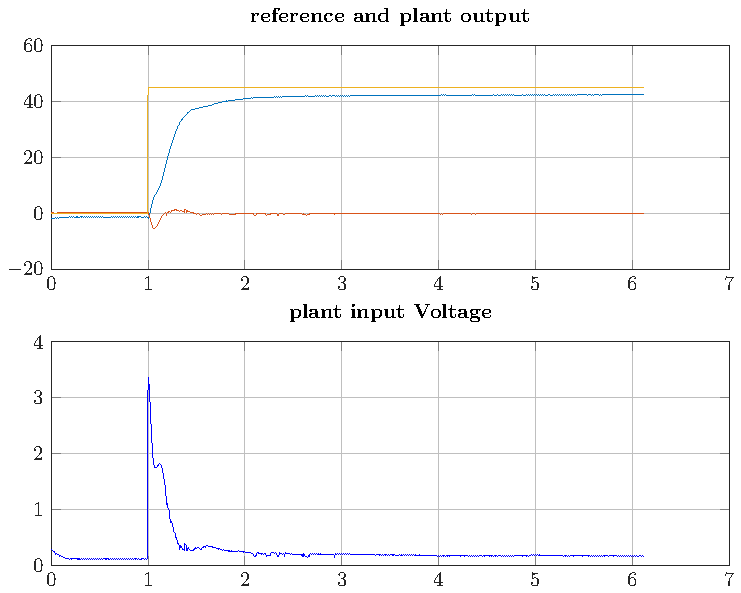
\includegraphics[scale = 0.46]{images/optimizedStepLab.pdf}
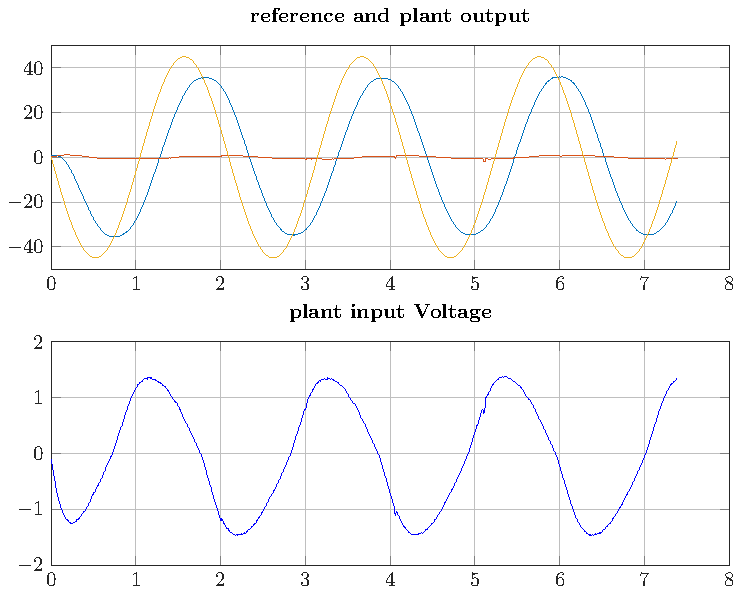
\includegraphics[scale = 0.46]{images/optimizedSineLab.pdf}
\caption{Setpoint tracking test results. References and plant outputs are given in degree [$\;^\circ$]. Plant input voltages are given in volts [V].}
\label{fig:setPoint}
\end{figure}
Using the controller we tuned during the simulation of our plant we started our experiments with some simple reference tracking experiments.\marginpar{Recall that we had the tuned controller: Q = diag([500 1000 3 10]) with R = 30.} The results are shown in figure~\ref{fig:setPoint}. In comparison to simulation~\ref{fig:allStates} results are as expected. The arm angle $\alpha$ oscillates a little less then expected. We observe a steady state offset that we did not see in our simulations, however this offset is within one or two degrees. Given that we have a small systematic error due to the potentiometer calibration that we did not fix completely this offset seems reasonable. We also applied a sinusoidal reference input. Tracking results are shown in figure~\ref{fig:allStates} on the right side. In comparison to the reference sine, which has an amplitude of $45^\circ$ our system output is damped. However in the beginning we stated that apart from good tracking results we also want our controller to keep the arm angle $\alpha$ as close to zero as possible. Again we are facing a conflicting control objectives. We cannot perfectly track the hub angle $\theta$ and keep the arm angle $\alpha$ close to zero. In our experiment the arm angle $\alpha$ remained within $2$ and $-2$ degrees at all times. If we tuned more towards tracking we would loose performance here. So we are proposing this controller as a compromise. 

\section{Disturbance Rejection}
\begin{figure}
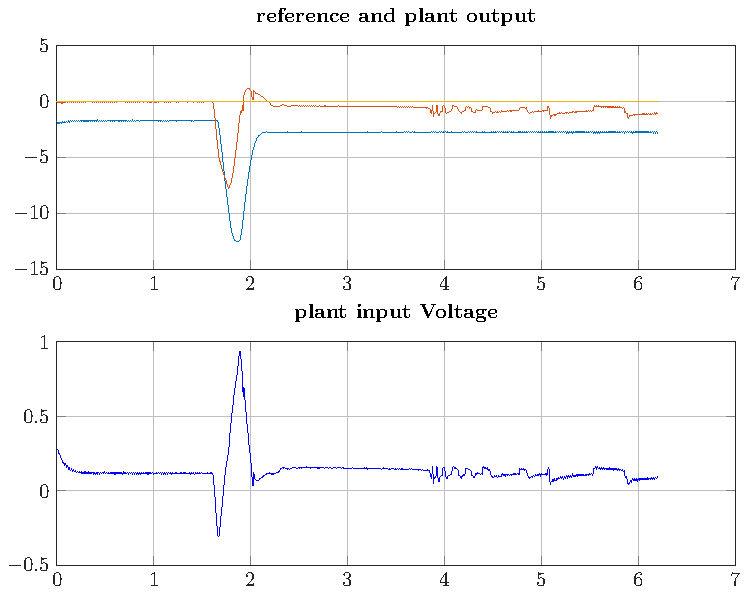
\includegraphics[scale = 0.65]{images/disturbance.pdf}
\caption{Plant and controller reaction to an external disturbance.}
\label{fig:disturbance}
\end{figure}
Next we are going to describe the results of some disturbance rejection tests. During these test we applied a small kick of $\approx 10^\circ$. Results are shown in figure~\ref{fig:disturbance}. After the disturbance the plant returns to its original position, with a small offset of about one degree. The input voltages remain withing the required bounds. It is important to note, that the reference remains zero at all times, since we are applying an external disturbance.

\section{The effect of removed arm angle feedback}
\begin{figure}
% This file was created by matlab2tikz v0.4.7 running on MATLAB 8.4.
% Copyright (c) 2008--2014, Nico Schlömer <nico.schloemer@gmail.com>
% All rights reserved.
% Minimal pgfplots version: 1.3
% 
% The latest updates can be retrieved from
%   http://www.mathworks.com/matlabcentral/fileexchange/22022-matlab2tikz
% where you can also make suggestions and rate matlab2tikz.
% 
\documentclass[tikz]{standalone}
\usepackage{pgfplots}
\usepackage{grffile}
\pgfplotsset{compat=newest}
\usetikzlibrary{plotmarks}
\usepackage{amsmath}

\begin{document}
%
% defining custom colors
\definecolor{mycolor1}{rgb}{0.00000,0.44700,0.74100}%
\definecolor{mycolor2}{rgb}{0.85000,0.32500,0.09800}%
\definecolor{mycolor3}{rgb}{0.92900,0.69400,0.12500}%
%
\begin{tikzpicture}

\begin{axis}[%
width=2in,
height=2in,
scale only axis,
separate axis lines,
every outer x axis line/.append style={white!15!black},
every x tick label/.append style={font=\color{white!15!black}},
xmin=0.741895261845386,
xmax=1.82668329177057,
xmajorgrids,
xlabel ={time in [s]},
every outer y axis line/.append style={white!15!black},
every y tick label/.append style={font=\color{white!15!black}},
ymin=-9,
ymax=6,
ymajorgrids,
ylabel={Arm angle $\alpha$ in [ $\;^\circ$]},
name=plot1,
title style={font=\bfseries},
title={Step response without feedback.}
]
\addplot [color=mycolor1,solid,forget plot]
  table[row sep=crcr]{0	-1.71029527278577\\
0.005	-1.71029527278577\\
0.01	-1.76239267728383\\
0.015	-1.84574852448072\\
0.02	-1.73113423458499\\
0.025	-1.66861734918733\\
0.03	-1.67903683008694\\
0.035	-1.69987579188616\\
0.04	-1.59568098289005\\
0.045	-1.49148617389394\\
0.05	-1.5540030592916\\
0.055	-1.57484202109083\\
0.06	-1.47064721209472\\
0.065	-1.40813032669705\\
0.07	-1.4602277311951\\
0.075	-1.49148617389394\\
0.08	-1.38729136489783\\
0.085	-1.29351603680133\\
0.09	-1.32477447950016\\
0.095	-1.3664524030986\\
0.1	-1.22057967050405\\
0.105	-1.13722382330716\\
0.11	-1.22057967050405\\
0.115	-1.23099915140366\\
0.12	-1.10596538060833\\
0.125	-1.04344849521066\\
0.13	-1.12680434240755\\
0.135	-1.14764330420677\\
0.14	-1.04344849521066\\
0.145	-0.96009264801377\\
0.15	-1.05386797611027\\
0.155	-1.0851264188091\\
0.16	-1.00177057161221\\
0.165	-0.907995243515715\\
0.17	-1.01219005251183\\
0.175	-1.07470693790949\\
0.18	-0.991351090712604\\
0.185	-0.907995243515715\\
0.19	-1.05386797611027\\
0.195	-1.10596538060833\\
0.2	-0.991351090712604\\
0.205	-0.939253686214548\\
0.21	-1.01219005251183\\
0.215	-1.0851264188091\\
0.22	-0.991351090712604\\
0.225	-0.918414724415326\\
0.23	-1.01219005251183\\
0.235	-1.06428745700988\\
0.24	-0.970512128913382\\
0.245	-0.897575762616104\\
0.25	-1.04344849521066\\
0.255	-1.0851264188091\\
0.26	-0.980931609812993\\
0.265	-0.918414724415326\\
0.27	-0.991351090712604\\
0.275	-1.07470693790949\\
0.28	-0.980931609812993\\
0.285	-0.928834205314937\\
0.29	-1.02260953341144\\
0.295	-1.07470693790949\\
0.3	-1.00177057161221\\
0.305	-0.939253686214548\\
0.31	-1.03302901431105\\
0.315	-1.0851264188091\\
0.32	-1.00177057161221\\
0.325	-0.939253686214548\\
0.33	-1.01219005251183\\
0.335	-1.09554589970872\\
0.34	-0.939253686214548\\
0.345	-0.939253686214548\\
0.35	-1.02260953341144\\
0.355	-1.06428745700988\\
0.36	-0.991351090712604\\
0.365	-0.949673167114159\\
0.37	-1.01219005251183\\
0.375	-1.06428745700988\\
0.38	-0.96009264801377\\
0.385	-0.928834205314937\\
0.39	-1.00177057161221\\
0.395	-1.0851264188091\\
0.4	-0.991351090712604\\
0.405	-0.918414724415326\\
0.41	-1.01219005251183\\
0.415	-1.06428745700988\\
0.42	-0.980931609812993\\
0.425	-0.907995243515715\\
0.43	-1.02260953341144\\
0.435	-1.06428745700988\\
0.44	-0.980931609812993\\
0.445	-0.928834205314937\\
0.45	-1.02260953341144\\
0.455	-1.07470693790949\\
0.46	-0.991351090712604\\
0.465	-0.928834205314937\\
0.47	-1.01219005251183\\
0.475	-1.05386797611027\\
0.48	-0.980931609812993\\
0.485	-0.928834205314937\\
0.49	-1.01219005251183\\
0.495	-1.06428745700988\\
0.5	-0.96009264801377\\
0.505	-0.928834205314937\\
0.51	-1.02260953341144\\
0.515	-1.06428745700988\\
0.52	-1.00177057161221\\
0.525	-0.939253686214548\\
0.53	-1.01219005251183\\
0.535	-1.09554589970872\\
0.54	-1.00177057161221\\
0.545	-0.928834205314937\\
0.55	-1.00177057161221\\
0.555	-1.0851264188091\\
0.56	-0.991351090712604\\
0.565	-0.939253686214548\\
0.57	-1.02260953341144\\
0.575	-1.09554589970872\\
0.58	-0.970512128913382\\
0.585	-0.928834205314937\\
0.59	-1.01219005251183\\
0.595	-1.06428745700988\\
0.6	-0.970512128913382\\
0.605	-0.918414724415326\\
0.61	-1.00177057161221\\
0.615	-1.06428745700988\\
0.62	-0.980931609812993\\
0.625	-0.918414724415326\\
0.63	-1.02260953341144\\
0.635	-1.06428745700988\\
0.64	-0.991351090712604\\
0.645	-0.949673167114159\\
0.65	-1.01219005251183\\
0.655	-1.07470693790949\\
0.66	-0.970512128913382\\
0.665	-0.939253686214548\\
0.67	-1.00177057161221\\
0.675	-1.06428745700988\\
0.68	-0.991351090712604\\
0.685	-0.918414724415326\\
0.69	-1.01219005251183\\
0.695	-1.09554589970872\\
0.7	-1.00177057161221\\
0.705	-0.918414724415326\\
0.71	-1.01219005251183\\
0.715	-1.07470693790949\\
0.72	-1.00177057161221\\
0.725	-0.939253686214548\\
0.73	-0.991351090712604\\
0.735	-1.0851264188091\\
0.74	-0.991351090712604\\
0.745	-0.939253686214548\\
0.75	-1.02260953341144\\
0.755	-1.07470693790949\\
0.76	-0.980931609812993\\
0.765	-0.918414724415326\\
0.77	-1.00177057161221\\
0.775	-1.07470693790949\\
0.78	-1.00177057161221\\
0.785	-0.928834205314937\\
0.79	-1.01219005251183\\
0.795	-1.06428745700988\\
0.8	-1.00177057161221\\
0.805	-0.96009264801377\\
0.81	-1.02260953341144\\
0.815	-1.0851264188091\\
0.82	-0.991351090712604\\
0.825	-0.949673167114159\\
0.83	-1.02260953341144\\
0.835	-1.0851264188091\\
0.84	-1.00177057161221\\
0.845	-0.928834205314937\\
0.85	-1.03302901431105\\
0.855	-1.06428745700988\\
0.86	-1.00177057161221\\
0.865	-0.949673167114159\\
0.87	-1.01219005251183\\
0.875	-1.09554589970872\\
0.88	-0.96009264801377\\
0.885	-0.939253686214548\\
0.89	-1.02260953341144\\
0.895	-1.0851264188091\\
0.9	-1.02260953341144\\
0.905	-0.928834205314937\\
0.91	-1.02260953341144\\
0.915	-1.07470693790949\\
0.92	-0.991351090712604\\
0.925	-0.928834205314937\\
0.93	-1.03302901431105\\
0.935	-1.07470693790949\\
0.94	-0.991351090712604\\
0.945	-0.939253686214548\\
0.95	-1.02260953341144\\
0.955	-1.05386797611027\\
0.96	-1.00177057161221\\
0.965	-0.928834205314937\\
0.97	-1.01219005251183\\
0.975	-1.06428745700988\\
0.98	-0.991351090712604\\
0.985	-0.949673167114159\\
0.99	-1.01219005251183\\
0.995	-1.0851264188091\\
1	-0.991351090712604\\
1.005	-1.86658748627994\\
1.01	-1.25183811320288\\
1.015	-0.324504313137492\\
1.02	0.863316509418178\\
1.025	2.15533214096996\\
1.03	3.40566984892329\\
1.035	4.61432963327819\\
1.04	5.86466734123152\\
1.045	6.93787387389147\\
1.05	7.89646611665569\\
1.055	8.70918562682536\\
1.06	9.55316357969386\\
1.065	10.2408493190682\\
1.07	10.6576285550526\\
1.075	11.0327298674386\\
1.08	11.5120259888208\\
1.085	11.9392247057048\\
1.09	12.1997117281951\\
1.095	12.4914571933842\\
1.1	12.9394948720675\\
1.105	13.3562741080519\\
1.11	13.6688585350403\\
1.115	14.0543793283259\\
1.12	14.6170312969049\\
1.125	15.1901027463835\\
1.13	15.6068819823679\\
1.135	16.1278560273485\\
1.14	16.8259612476224\\
1.145	17.5761638723944\\
1.15	18.1804937645719\\
1.155	18.847340542147\\
1.16	19.7434158995135\\
1.165	20.6290717759805\\
1.17	21.473049728849\\
1.175	22.1607354682233\\
1.18	22.9526160165938\\
1.185	23.7861744885627\\
1.19	24.3384069762421\\
1.195	24.9323173875199\\
1.2	25.7137784549907\\
1.205	26.4014641943651\\
1.21	26.9953746056429\\
1.215	27.5788655360211\\
1.22	28.2873902371947\\
1.225	28.9333980529706\\
1.23	29.4022746934531\\
1.235	29.9024097766344\\
1.24	30.475481226113\\
1.245	31.1006500800897\\
1.25	31.4965903542749\\
1.255	31.9446280329582\\
1.26	32.486441039738\\
1.265	32.9865761229193\\
1.27	33.3304189926065\\
1.275	33.5804865341971\\
1.28	34.0285242128804\\
1.285	34.414045006166\\
1.29	34.6224346241582\\
1.295	34.8099852803512\\
1.3	35.164247630938\\
1.305	35.4664125770267\\
1.31	35.5601879051233\\
1.315	35.7581580422159\\
1.32	36.0082255838065\\
1.325	36.2999710489956\\
1.33	36.3520684534937\\
1.335	36.4562632624898\\
1.34	36.6542333995824\\
1.345	36.852203536675\\
1.35	36.8626230175746\\
1.355	36.8730424984742\\
1.36	37.0814321164665\\
1.365	37.2481438108602\\
1.37	37.2481438108602\\
1.375	37.2168853681614\\
1.38	37.3210801771575\\
1.385	37.3731775816556\\
1.39	37.2585632917599\\
1.395	37.175207444563\\
1.4	37.2689827726595\\
1.405	37.3314996580571\\
1.41	37.2481438108602\\
1.415	37.1960464063622\\
1.42	37.3002412153583\\
1.425	37.3210801771575\\
1.43	37.227304849061\\
1.435	37.1856269254626\\
1.44	37.2689827726595\\
1.445	37.3106606962579\\
1.45	37.2168853681614\\
1.455	37.1543684827638\\
1.46	37.2481438108602\\
1.465	37.2585632917599\\
1.47	37.2168853681614\\
1.475	37.1439490018641\\
1.48	37.2168853681614\\
1.485	37.2689827726595\\
1.49	37.1960464063622\\
1.495	37.1543684827638\\
1.5	37.2377243299606\\
1.505	37.3314996580571\\
1.51	37.2794022535591\\
1.515	37.2689827726595\\
1.52	37.3940165434548\\
1.525	37.4773723906517\\
1.53	37.4669529097521\\
1.535	37.4773723906517\\
1.54	37.6440840850455\\
1.545	37.8003762985396\\
1.55	37.8107957794393\\
1.555	37.8316347412385\\
1.56	38.0296048783311\\
1.565	38.1858970918252\\
1.57	38.1754776109256\\
1.575	38.2275750154237\\
1.58	38.4151256716167\\
1.585	38.5505789233116\\
1.59	38.5922568469101\\
1.595	38.6443542514081\\
1.6	38.8527438694004\\
1.605	39.0298750446938\\
1.61	39.050714006493\\
1.615	39.0819724491918\\
1.62	39.2591036244852\\
1.625	39.425815318879\\
1.63	39.4153958379794\\
1.635	39.477912723377\\
1.64	39.6550438986704\\
1.645	39.8321750739638\\
1.65	39.8217555930642\\
1.655	39.8738529975623\\
1.66	40.0718231346549\\
1.665	40.2072763863498\\
1.67	40.2072763863498\\
1.675	40.2697932717475\\
1.68	40.4469244470409\\
1.685	40.6136361414346\\
1.69	40.5615387369366\\
1.695	40.5823776987358\\
1.7	40.7490893931296\\
1.705	40.8637036830253\\
1.71	40.8324452403265\\
1.715	40.8428647212261\\
1.72	40.978317972921\\
1.725	41.1033517437164\\
1.73	41.0408348583187\\
1.735	41.0304153774191\\
1.74	41.1554491482144\\
1.745	41.2179660336121\\
1.75	41.1971270718129\\
1.755	41.1554491482144\\
1.76	41.2909023999094\\
1.765	41.3742582471063\\
1.77	41.3221608426082\\
1.775	41.2700634381101\\
1.78	41.353419285307\\
1.785	41.4471946134035\\
1.79	41.3325803235078\\
1.795	41.3221608426082\\
1.8	41.4471946134035\\
1.805	41.5097114988012\\
1.81	41.4263556516043\\
1.815	41.3846777280059\\
1.82	41.488872537002\\
1.825	41.5722283841989\\
1.83	41.488872537002\\
1.835	41.4367751325039\\
1.84	41.5513894223996\\
1.845	41.6243257886969\\
1.85	41.5618089032993\\
1.855	41.4992920179016\\
1.86	41.5930673459981\\
1.865	41.676423193195\\
1.87	41.6034868268977\\
1.875	41.5618089032993\\
1.88	41.6660037122954\\
1.885	41.728520597693\\
1.89	41.6660037122954\\
1.895	41.5930673459981\\
1.9	41.676423193195\\
1.905	41.7597790403919\\
1.91	41.6868426740946\\
1.915	41.6555842313958\\
1.92	41.7701985212915\\
1.925	41.8431348875888\\
1.93	41.7806180021911\\
1.935	41.728520597693\\
1.94	41.8014569639903\\
1.945	41.8848128111872\\
1.95	41.8014569639903\\
1.955	41.7806180021911\\
1.96	41.8743933302876\\
1.965	41.9369102156853\\
1.97	41.8952322920868\\
1.975	41.8327154066891\\
1.98	41.916071253886\\
1.985	41.9994271010829\\
1.99	41.9577491774845\\
1.995	41.8743933302876\\
2	41.9890076201833\\
2.005	42.0827829482798\\
2.01	41.9681686583841\\
2.015	41.9369102156853\\
2.02	42.0306855437818\\
2.025	42.103621910079\\
2.03	42.051524505581\\
2.035	41.9890076201833\\
2.04	42.0723634673802\\
2.045	42.1452998336775\\
2.05	42.0827829482798\\
2.055	42.051524505581\\
2.06	42.1348803527779\\
2.065	42.1973972381755\\
2.07	42.1244608718783\\
2.075	42.0827829482798\\
2.08	42.1765582763763\\
2.085	42.2494946426736\\
2.09	42.1765582763763\\
2.095	42.1244608718783\\
2.1	42.2182361999748\\
2.105	42.2807530853724\\
2.11	42.2182361999748\\
2.115	42.1765582763763\\
2.12	42.2286556808744\\
2.125	42.2807530853724\\
2.13	42.2286556808744\\
2.135	42.1765582763763\\
2.14	42.2599141235732\\
2.145	42.3328504898705\\
2.15	42.2494946426736\\
2.155	42.2182361999748\\
2.16	42.291172566272\\
2.165	42.3641089325693\\
2.17	42.2807530853724\\
2.175	42.2494946426736\\
2.18	42.3328504898705\\
2.185	42.4057868561678\\
2.19	42.3224310089709\\
2.195	42.2807530853724\\
2.2	42.3536894516697\\
2.205	42.4370452988666\\
2.21	42.3641089325693\\
2.215	42.3224310089709\\
2.22	42.3953673752682\\
2.225	42.4474647797662\\
2.23	42.3953673752682\\
2.235	42.3328504898705\\
2.24	42.4162063370674\\
2.245	42.478723222465\\
2.25	42.4162063370674\\
2.255	42.3536894516697\\
2.26	42.4474647797662\\
2.265	42.5204011460635\\
2.27	42.4370452988666\\
2.275	42.3641089325693\\
2.28	42.4474647797662\\
2.285	42.5412401078627\\
2.29	42.426625817967\\
2.295	42.3745284134689\\
2.3	42.478723222465\\
2.305	42.5724985505615\\
2.31	42.4370452988666\\
2.315	42.4162063370674\\
2.32	42.4891427033646\\
2.325	42.5308206269631\\
2.33	42.478723222465\\
2.335	42.4162063370674\\
2.34	42.5308206269631\\
2.345	42.5724985505615\\
2.35	42.478723222465\\
2.355	42.426625817967\\
2.36	42.5412401078627\\
2.365	42.5724985505615\\
2.37	42.5099816651639\\
2.375	42.4683037415654\\
2.38	42.5516595887623\\
2.385	42.5933375123608\\
2.39	42.5308206269631\\
2.395	42.4995621842643\\
2.4	42.5829180314611\\
2.405	42.6245959550596\\
2.41	42.5412401078627\\
2.415	42.4891427033646\\
2.42	42.5829180314611\\
2.425	42.6350154359592\\
2.43	42.5308206269631\\
2.435	42.4995621842643\\
2.44	42.5933375123608\\
2.445	42.6558543977584\\
2.45	42.5724985505615\\
2.455	42.4995621842643\\
2.46	42.5829180314611\\
2.465	42.666273878658\\
2.47	42.5829180314611\\
2.475	42.5099816651639\\
2.48	42.6037569932604\\
2.485	42.6454349168588\\
2.49	42.5620790696619\\
2.495	42.5204011460635\\
2.5	42.61417647416\\
2.505	42.7079518022565\\
2.51	42.5933375123608\\
2.515	42.5412401078627\\
2.52	42.6245959550596\\
2.525	42.7079518022565\\
2.53	42.6245959550596\\
2.535	42.5620790696619\\
2.54	42.6558543977584\\
2.545	42.7287907640557\\
2.55	42.6350154359592\\
2.555	42.5933375123608\\
2.56	42.666273878658\\
2.565	42.7183712831561\\
2.57	42.6350154359592\\
2.575	42.6037569932604\\
2.58	42.6871128404573\\
2.585	42.7392102449553\\
2.59	42.6454349168588\\
2.595	42.61417647416\\
2.6	42.7079518022565\\
2.605	42.7496297258549\\
2.61	42.6766933595576\\
2.615	42.61417647416\\
2.62	42.6871128404573\\
2.625	42.7600492067545\\
2.63	42.6766933595576\\
2.635	42.61417647416\\
2.64	42.6975323213569\\
2.645	42.7600492067545\\
2.65	42.6975323213569\\
2.655	42.6245959550596\\
2.66	42.7287907640557\\
2.665	42.7704686876542\\
2.67	42.6975323213569\\
2.675	42.6558543977584\\
2.68	42.6975323213569\\
2.685	42.7704686876542\\
2.69	42.7079518022565\\
2.695	42.6350154359592\\
2.7	42.7496297258549\\
2.705	42.7808881685538\\
2.71	42.6975323213569\\
2.715	42.6454349168588\\
2.72	42.7183712831561\\
2.725	42.801727130353\\
2.73	42.7079518022565\\
2.735	42.6558543977584\\
2.74	42.7392102449553\\
2.745	42.7808881685538\\
2.75	42.7183712831561\\
2.755	42.666273878658\\
2.76	42.7704686876542\\
2.765	42.7913076494534\\
2.77	42.6975323213569\\
2.775	42.666273878658\\
2.78	42.7392102449553\\
2.785	42.7808881685538\\
2.79	42.7079518022565\\
2.795	42.666273878658\\
2.8	42.7808881685538\\
2.805	42.8121466112526\\
2.81	42.7183712831561\\
2.815	42.6766933595576\\
2.82	42.7600492067545\\
2.825	42.7913076494534\\
2.83	42.7287907640557\\
2.835	42.6871128404573\\
2.84	42.7808881685538\\
2.845	42.8225660921522\\
2.85	42.7496297258549\\
2.855	42.6871128404573\\
2.86	42.7704686876542\\
2.865	42.8121466112526\\
2.87	42.7704686876542\\
2.875	42.6975323213569\\
2.88	42.7600492067545\\
2.885	42.8329855730518\\
2.89	42.7496297258549\\
2.895	42.7079518022565\\
2.9	42.7913076494534\\
2.905	42.8225660921522\\
2.91	42.7392102449553\\
2.915	42.7079518022565\\
2.92	42.801727130353\\
2.925	42.8434050539514\\
2.93	42.7704686876542\\
2.935	42.7183712831561\\
2.94	42.7913076494534\\
2.945	42.8434050539514\\
2.95	42.7913076494534\\
2.955	42.7079518022565\\
2.96	42.7808881685538\\
2.965	42.8225660921522\\
2.97	42.7392102449553\\
2.975	42.7079518022565\\
2.98	42.801727130353\\
2.985	42.853824534851\\
2.99	42.7808881685538\\
2.995	42.7496297258549\\
3	42.801727130353\\
3.005	42.8642440157506\\
3.01	42.7704686876542\\
3.015	42.7392102449553\\
3.02	42.7913076494534\\
3.025	42.8746634966503\\
3.03	42.7808881685538\\
3.035	42.7392102449553\\
3.04	42.8121466112526\\
3.045	42.853824534851\\
3.05	42.7913076494534\\
3.055	42.7496297258549\\
3.06	42.801727130353\\
3.065	42.8850829775499\\
3.07	42.7913076494534\\
3.075	42.7287907640557\\
3.08	42.8121466112526\\
3.085	42.8642440157506\\
3.09	42.7913076494534\\
3.095	42.7287907640557\\
3.1	42.8121466112526\\
3.105	42.8955024584495\\
3.11	42.7808881685538\\
3.115	42.7496297258549\\
3.12	42.8329855730518\\
3.125	42.9059219393491\\
3.13	42.801727130353\\
3.135	42.7496297258549\\
3.14	42.8329855730518\\
3.145	42.8850829775499\\
3.15	42.801727130353\\
3.155	42.7496297258549\\
3.16	42.8329855730518\\
3.165	42.8850829775499\\
3.17	42.8225660921522\\
3.175	42.7704686876542\\
3.18	42.8329855730518\\
3.185	42.8955024584495\\
3.19	42.8121466112526\\
3.195	42.7496297258549\\
3.2	42.8434050539514\\
3.205	42.9059219393491\\
3.21	42.8225660921522\\
3.215	42.7600492067545\\
3.22	42.8434050539514\\
3.225	42.9163414202487\\
3.23	42.8329855730518\\
3.235	42.7808881685538\\
3.24	42.853824534851\\
3.245	42.9163414202487\\
3.25	42.8329855730518\\
3.255	42.7704686876542\\
3.26	42.8225660921522\\
3.265	42.8955024584495\\
3.27	42.8225660921522\\
3.275	42.7808881685538\\
3.28	42.8434050539514\\
3.285	42.9163414202487\\
3.29	42.8434050539514\\
3.295	42.7913076494534\\
3.3	42.8746634966503\\
3.305	42.9267609011483\\
3.31	42.8225660921522\\
3.315	42.7913076494534\\
3.32	42.8642440157506\\
3.325	42.9059219393491\\
3.33	42.8434050539514\\
3.335	42.7600492067545\\
3.34	42.853824534851\\
3.345	42.9267609011483\\
3.35	42.8434050539514\\
3.355	42.7600492067545\\
3.36	42.8434050539514\\
3.365	42.8850829775499\\
3.37	42.8225660921522\\
3.375	42.7496297258549\\
3.38	42.8642440157506\\
3.385	42.9371803820479\\
3.39	42.8329855730518\\
3.395	42.7808881685538\\
3.4	42.8642440157506\\
3.405	42.9267609011483\\
3.41	42.8434050539514\\
3.415	42.7808881685538\\
3.42	42.8434050539514\\
3.425	42.8955024584495\\
3.43	42.8329855730518\\
3.435	42.7913076494534\\
3.44	42.853824534851\\
3.445	42.9163414202487\\
3.45	42.853824534851\\
3.455	42.7496297258549\\
3.46	42.853824534851\\
3.465	42.9163414202487\\
3.47	42.8329855730518\\
3.475	42.7808881685538\\
3.48	42.8850829775499\\
3.485	42.9059219393491\\
3.49	42.8329855730518\\
3.495	42.7808881685538\\
3.5	42.8642440157506\\
3.505	42.9267609011483\\
3.51	42.8434050539514\\
3.515	42.7913076494534\\
3.52	42.8746634966503\\
3.525	42.9267609011483\\
3.53	42.8329855730518\\
3.535	42.7913076494534\\
3.54	42.8434050539514\\
3.545	42.9059219393491\\
3.55	42.8225660921522\\
3.555	42.7913076494534\\
3.56	42.8642440157506\\
3.565	42.9163414202487\\
3.57	42.8642440157506\\
3.575	42.7913076494534\\
3.58	42.8434050539514\\
3.585	42.9059219393491\\
3.59	42.8329855730518\\
3.595	42.7913076494534\\
3.6	42.8746634966503\\
3.605	42.9267609011483\\
3.61	42.8225660921522\\
3.615	42.7808881685538\\
3.62	42.8955024584495\\
3.625	42.8955024584495\\
3.63	42.8329855730518\\
3.635	42.7808881685538\\
3.64	42.853824534851\\
3.645	42.9371803820479\\
3.65	42.8329855730518\\
3.655	42.7808881685538\\
3.66	42.8850829775499\\
3.665	42.9267609011483\\
3.67	42.8329855730518\\
3.675	42.7808881685538\\
3.68	42.8642440157506\\
3.685	42.9267609011483\\
3.69	42.8434050539514\\
3.695	42.801727130353\\
3.7	42.8746634966503\\
3.705	42.9163414202487\\
3.71	42.8434050539514\\
3.715	42.7913076494534\\
3.72	42.8746634966503\\
3.725	42.9267609011483\\
3.73	42.8434050539514\\
3.735	42.7913076494534\\
3.74	42.853824534851\\
3.745	42.9267609011483\\
3.75	42.8329855730518\\
3.755	42.801727130353\\
3.76	42.8746634966503\\
3.765	42.9267609011483\\
3.77	42.853824534851\\
3.775	42.801727130353\\
3.78	42.8850829775499\\
3.785	42.9163414202487\\
3.79	42.8225660921522\\
3.795	42.7913076494534\\
3.8	42.8642440157506\\
3.805	42.9267609011483\\
3.81	42.853824534851\\
3.815	42.7913076494534\\
3.82	42.8434050539514\\
3.825	42.9163414202487\\
3.83	42.8121466112526\\
3.835	42.7913076494534\\
3.84	42.8955024584495\\
3.845	42.9267609011483\\
3.85	42.8225660921522\\
3.855	42.801727130353\\
3.86	42.8955024584495\\
3.865	42.9267609011483\\
3.87	42.853824534851\\
3.875	42.801727130353\\
3.88	42.8850829775499\\
3.885	42.9163414202487\\
3.89	42.8434050539514\\
3.895	42.7808881685538\\
3.9	42.8850829775499\\
3.905	42.9371803820479\\
3.91	42.8434050539514\\
3.915	42.8121466112526\\
3.92	42.9059219393491\\
3.925	42.9163414202487\\
3.93	42.853824534851\\
3.935	42.7808881685538\\
3.94	42.8642440157506\\
3.945	42.9163414202487\\
3.95	42.853824534851\\
3.955	42.7913076494534\\
3.96	42.853824534851\\
3.965	42.9371803820479\\
3.97	42.8434050539514\\
3.975	42.7808881685538\\
3.98	42.853824534851\\
3.985	42.9267609011483\\
3.99	42.8329855730518\\
3.995	42.801727130353\\
4	42.853824534851\\
4.005	42.9371803820479\\
4.01	42.853824534851\\
4.015	42.7913076494534\\
4.02	42.8642440157506\\
4.025	42.9580193438471\\
4.03	42.8329855730518\\
4.035	42.7913076494534\\
4.04	42.8955024584495\\
4.045	42.9267609011483\\
4.05	42.8434050539514\\
4.055	42.7913076494534\\
4.06	42.8850829775499\\
4.065	42.9267609011483\\
4.07	42.8434050539514\\
4.075	42.7913076494534\\
4.08	42.8746634966503\\
4.085	42.9267609011483\\
4.09	42.8434050539514\\
4.095	42.7808881685538\\
4.1	42.8850829775499\\
4.105	42.9371803820479\\
4.11	42.8434050539514\\
4.115	42.8121466112526\\
4.12	42.9059219393491\\
4.125	42.9267609011483\\
4.13	42.8434050539514\\
4.135	42.8225660921522\\
4.14	42.8955024584495\\
4.145	42.9267609011483\\
4.15	42.853824534851\\
4.155	42.801727130353\\
4.16	42.9059219393491\\
4.165	42.9267609011483\\
4.17	42.853824534851\\
4.175	42.8329855730518\\
4.18	42.8850829775499\\
4.185	42.9475998629475\\
4.19	42.8434050539514\\
4.195	42.8225660921522\\
4.2	42.8850829775499\\
4.205	42.9475998629475\\
4.21	42.8850829775499\\
4.215	42.801727130353\\
4.22	42.9059219393491\\
4.225	42.9475998629475\\
4.23	42.853824534851\\
4.235	42.801727130353\\
4.24	42.8850829775499\\
4.245	42.9371803820479\\
4.25	42.8642440157506\\
4.255	42.801727130353\\
4.26	42.8850829775499\\
4.265	42.9371803820479\\
4.27	42.853824534851\\
4.275	42.8121466112526\\
4.28	42.8955024584495\\
4.285	42.9371803820479\\
4.29	42.8434050539514\\
4.295	42.8121466112526\\
4.3	42.8746634966503\\
4.305	42.9059219393491\\
4.31	42.853824534851\\
4.315	42.8121466112526\\
4.32	42.8746634966503\\
4.325	42.9371803820479\\
4.33	42.8642440157506\\
4.335	42.801727130353\\
4.34	42.9059219393491\\
4.345	42.9475998629475\\
4.35	42.853824534851\\
4.355	42.7913076494534\\
4.36	42.8642440157506\\
4.365	42.9267609011483\\
4.37	42.853824534851\\
4.375	42.801727130353\\
4.38	42.8642440157506\\
4.385	42.9371803820479\\
4.39	42.8746634966503\\
4.395	42.8121466112526\\
4.4	42.8850829775499\\
4.405	42.9371803820479\\
4.41	42.8329855730518\\
4.415	42.8121466112526\\
4.42	42.8955024584495\\
4.425	42.9475998629475\\
4.43	42.853824534851\\
4.435	42.8121466112526\\
4.44	42.8850829775499\\
4.445	42.9475998629475\\
4.45	42.853824534851\\
4.455	42.8329855730518\\
4.46	42.8955024584495\\
4.465	42.9163414202487\\
4.47	42.8434050539514\\
4.475	42.8121466112526\\
4.48	42.9059219393491\\
4.485	42.9267609011483\\
4.49	42.8434050539514\\
4.495	42.8121466112526\\
4.5	42.8850829775499\\
4.505	42.9267609011483\\
4.51	42.853824534851\\
4.515	42.801727130353\\
4.52	42.8955024584495\\
4.525	42.9475998629475\\
4.53	42.8746634966503\\
4.535	42.8225660921522\\
4.54	42.8955024584495\\
4.545	42.9267609011483\\
4.55	42.8850829775499\\
4.555	42.8434050539514\\
4.56	42.8955024584495\\
4.565	42.9475998629475\\
4.57	42.853824534851\\
4.575	42.801727130353\\
4.58	42.8850829775499\\
4.585	42.9371803820479\\
4.59	42.8434050539514\\
4.595	42.8225660921522\\
4.6	42.8746634966503\\
4.605	42.9371803820479\\
4.61	42.8642440157506\\
4.615	42.8225660921522\\
4.62	42.8746634966503\\
4.625	42.9371803820479\\
4.63	42.8329855730518\\
4.635	42.801727130353\\
4.64	42.8955024584495\\
4.645	42.9580193438471\\
4.65	42.853824534851\\
4.655	42.8121466112526\\
4.66	42.8434050539514\\
4.665	42.9059219393491\\
4.67	42.853824534851\\
4.675	42.8225660921522\\
4.68	42.8850829775499\\
4.685	42.9163414202487\\
4.69	42.8434050539514\\
4.695	42.8225660921522\\
4.7	42.8955024584495\\
4.705	42.9267609011483\\
4.71	42.8850829775499\\
4.715	42.801727130353\\
4.72	42.8850829775499\\
4.725	42.9475998629475\\
4.73	42.853824534851\\
4.735	42.801727130353\\
4.74	42.8746634966503\\
4.745	42.9267609011483\\
4.75	42.8850829775499\\
4.755	42.8329855730518\\
4.76	42.8746634966503\\
4.765	42.9475998629475\\
4.77	42.8642440157506\\
4.775	42.8121466112526\\
4.78	42.8746634966503\\
4.785	42.9267609011483\\
4.79	42.853824534851\\
4.795	42.8225660921522\\
};
\addplot [color=mycolor2,solid,forget plot]
  table[row sep=crcr]{0	-0.0299970263147632\\
0.005	-0.0256571787576505\\
0.01	-0.0820751970001161\\
0.015	-0.116793977457018\\
0.02	-0.0560361116574397\\
0.025	-0.0820751970001161\\
0.03	-0.194911233485047\\
0.035	-0.264348794398851\\
0.04	-0.233969861499062\\
0.045	-0.212270623713498\\
0.05	-0.2469894041704\\
0.055	-0.212270623713498\\
0.06	-0.0603759592145524\\
0.065	0.000381906585025969\\
0.07	-0.0430165689861015\\
0.075	-0.0647158067716651\\
0.08	0.000381906585025969\\
0.085	0.0307608394848152\\
0.09	-0.0213173312005377\\
0.095	-0.0560361116574397\\
0.1	0.000381906585025969\\
0.105	0.0437803821561534\\
0.11	-0.0126376360863123\\
0.115	-0.0430165689861015\\
0.12	0.00472175414213871\\
0.125	0.0481202297132661\\
0.13	-0.00829778852919952\\
0.135	-0.034336873871876\\
0.14	0.0134014492563642\\
0.145	0.0567999248274916\\
0.15	0.000381906585025969\\
0.155	-0.0213173312005377\\
0.16	0.0394405345990406\\
0.165	0.0741593150559426\\
0.17	0.0134014492563642\\
0.175	-0.016977483643425\\
0.18	0.0351006870419279\\
0.185	0.0611397723846044\\
0.19	0.00472175414213871\\
0.195	-0.0386767214289887\\
0.2	0.000381906585025969\\
0.205	0.00472175414213871\\
0.21	-0.0690556543287779\\
0.215	-0.116793977457018\\
0.22	-0.0820751970001161\\
0.225	-0.0430165689861015\\
0.23	-0.121133825014131\\
0.235	-0.147172910356807\\
0.24	-0.0950947396714543\\
0.245	-0.0560361116574397\\
0.25	-0.10377443478568\\
0.255	-0.147172910356807\\
0.26	-0.0733955018858907\\
0.265	-0.0256571787576505\\
0.27	-0.0733955018858907\\
0.275	-0.0994345872285671\\
0.28	-0.034336873871876\\
0.285	0.000381906585025969\\
0.29	-0.0560361116574397\\
0.295	-0.0864150445572289\\
0.3	-0.034336873871876\\
0.305	-0.00395794097208677\\
0.31	-0.0690556543287779\\
0.315	-0.112454129899905\\
0.32	-0.0560361116574397\\
0.325	-0.034336873871876\\
0.33	-0.0864150445572289\\
0.335	-0.121133825014131\\
0.34	-0.0647158067716651\\
0.345	-0.0299970263147632\\
0.35	-0.0733955018858907\\
0.355	-0.10377443478568\\
0.36	-0.0473564165432142\\
0.365	-0.0213173312005377\\
0.37	-0.0690556543287779\\
0.375	-0.10377443478568\\
0.38	-0.0430165689861015\\
0.385	-0.0126376360863123\\
0.39	-0.0647158067716651\\
0.395	-0.10377443478568\\
0.4	-0.0560361116574397\\
0.405	-0.0213173312005377\\
0.41	-0.0820751970001161\\
0.415	-0.112454129899905\\
0.42	-0.0516962641003269\\
0.425	-0.0256571787576505\\
0.43	-0.0820751970001161\\
0.435	-0.112454129899905\\
0.44	-0.0560361116574397\\
0.445	-0.0213173312005377\\
0.45	-0.0647158067716651\\
0.455	-0.108114282342793\\
0.46	-0.0516962641003269\\
0.465	-0.00829778852919952\\
0.47	-0.0690556543287779\\
0.475	-0.0994345872285671\\
0.48	-0.0473564165432142\\
0.485	-0.0213173312005377\\
0.49	-0.0733955018858907\\
0.495	-0.112454129899905\\
0.5	-0.0560361116574397\\
0.505	-0.016977483643425\\
0.51	-0.0820751970001161\\
0.515	-0.10377443478568\\
0.52	-0.0603759592145524\\
0.525	-0.0256571787576505\\
0.53	-0.0733955018858907\\
0.535	-0.10377443478568\\
0.54	-0.0560361116574397\\
0.545	-0.0256571787576505\\
0.55	-0.0733955018858907\\
0.555	-0.108114282342793\\
0.56	-0.0560361116574397\\
0.565	-0.0299970263147632\\
0.57	-0.0777353494430034\\
0.575	-0.121133825014131\\
0.58	-0.0603759592145524\\
0.585	-0.0213173312005377\\
0.59	-0.0820751970001161\\
0.595	-0.108114282342793\\
0.6	-0.0560361116574397\\
0.605	-0.0256571787576505\\
0.61	-0.0733955018858907\\
0.615	-0.112454129899905\\
0.62	-0.0516962641003269\\
0.625	-0.0256571787576505\\
0.63	-0.0733955018858907\\
0.635	-0.112454129899905\\
0.64	-0.0603759592145524\\
0.645	-0.0213173312005377\\
0.65	-0.0777353494430034\\
0.655	-0.121133825014131\\
0.66	-0.0603759592145524\\
0.665	-0.0256571787576505\\
0.67	-0.0777353494430034\\
0.675	-0.112454129899905\\
0.68	-0.0647158067716651\\
0.685	-0.0256571787576505\\
0.69	-0.0820751970001161\\
0.695	-0.108114282342793\\
0.7	-0.0603759592145524\\
0.705	-0.0299970263147632\\
0.71	-0.0690556543287779\\
0.715	-0.112454129899905\\
0.72	-0.0473564165432142\\
0.725	-0.0213173312005377\\
0.73	-0.0733955018858907\\
0.735	-0.10377443478568\\
0.74	-0.0560361116574397\\
0.745	-0.0299970263147632\\
0.75	-0.0733955018858907\\
0.755	-0.10377443478568\\
0.76	-0.0603759592145524\\
0.765	-0.016977483643425\\
0.77	-0.0777353494430034\\
0.775	-0.10377443478568\\
0.78	-0.0603759592145524\\
0.785	-0.0256571787576505\\
0.79	-0.0690556543287779\\
0.795	-0.112454129899905\\
0.8	-0.0560361116574397\\
0.805	-0.0386767214289887\\
0.81	-0.0733955018858907\\
0.815	-0.112454129899905\\
0.82	-0.0560361116574397\\
0.825	-0.0256571787576505\\
0.83	-0.0733955018858907\\
0.835	-0.112454129899905\\
0.84	-0.0647158067716651\\
0.845	-0.0256571787576505\\
0.85	-0.0864150445572289\\
0.855	-0.116793977457018\\
0.86	-0.0647158067716651\\
0.865	-0.0213173312005377\\
0.87	-0.0733955018858907\\
0.875	-0.108114282342793\\
0.88	-0.0516962641003269\\
0.885	-0.0213173312005377\\
0.89	-0.0777353494430034\\
0.895	-0.112454129899905\\
0.9	-0.0690556543287779\\
0.905	-0.0256571787576505\\
0.91	-0.0733955018858907\\
0.915	-0.10377443478568\\
0.92	-0.0560361116574397\\
0.925	-0.0256571787576505\\
0.93	-0.0733955018858907\\
0.935	-0.112454129899905\\
0.94	-0.0603759592145524\\
0.945	-0.0256571787576505\\
0.95	-0.0777353494430034\\
0.955	-0.116793977457018\\
0.96	-0.0603759592145524\\
0.965	-0.0126376360863123\\
0.97	-0.0777353494430034\\
0.975	-0.0994345872285671\\
0.98	-0.0560361116574397\\
0.985	-0.0213173312005377\\
0.99	-0.0777353494430034\\
0.995	-0.112454129899905\\
1	-0.0560361116574397\\
1.005	-0.542099038054067\\
1.01	-1.15835739116408\\
1.015	-1.90047132343036\\
1.02	-2.75108144462445\\
1.025	-3.70150805963214\\
1.03	-4.75175116845343\\
1.035	-5.80199427727471\\
1.04	-6.68732317892571\\
1.045	-7.43811680630621\\
1.05	-8.13683226300136\\
1.055	-8.65327412229778\\
1.06	-8.88762589038187\\
1.065	-8.97876268908124\\
1.07	-8.83554771969652\\
1.075	-8.68365305519757\\
1.08	-8.32778555551432\\
1.085	-7.86776171446037\\
1.09	-7.41641756852065\\
1.095	-6.86525692876733\\
1.1	-6.17522116718641\\
1.105	-5.44612677759146\\
1.11	-4.812509034253\\
1.115	-4.15285220557187\\
1.12	-3.44545705376249\\
1.125	-2.7684408348529\\
1.13	-2.17822156708557\\
1.135	-1.53158428107577\\
1.14	-0.924005623079988\\
1.145	-0.533419342939841\\
1.15	-0.776450806138155\\
1.155	0.0524600772703789\\
1.16	0.620980107252148\\
1.165	0.981187454492506\\
1.17	1.31101586883307\\
1.175	1.64518413073076\\
1.18	2.0357704108709\\
1.185	2.42635669101105\\
1.19	2.6824076968807\\
1.195	2.96883763565014\\
1.2	3.30734574510494\\
1.205	3.58075614120304\\
1.21	3.75001019593044\\
1.215	3.94530333600051\\
1.22	4.25343251255551\\
1.225	4.51382336598228\\
1.23	4.57024138422474\\
1.235	4.60062031712453\\
1.24	4.33154976858354\\
1.245	4.7611946767377\\
1.25	4.11889723828502\\
1.255	5.11706217642095\\
1.26	5.0997027861925\\
1.265	5.0649840057356\\
1.27	4.93912842657933\\
1.275	4.84799162787996\\
1.28	4.80893299986594\\
1.285	4.73515559139503\\
1.29	4.56156168911052\\
1.295	4.34890915881199\\
1.3	4.23173327476995\\
1.305	4.12323708584213\\
1.31	3.88888531775804\\
1.315	3.64151400700262\\
1.32	3.48527949494656\\
1.325	3.29866604999071\\
1.33	3.00355641610704\\
1.335	2.72580617245183\\
1.34	2.48277470925351\\
1.345	2.24842294116943\\
1.35	1.90557498415752\\
1.355	1.60178565515963\\
1.36	1.41517221020378\\
1.365	1.12440242387723\\
1.37	0.79891385709377\\
1.375	0.495124528095879\\
1.38	0.317190778254256\\
1.385	0.139257028412634\\
1.39	-0.134153367685469\\
1.395	-0.37284498332667\\
1.4	-0.56379827583963\\
1.405	-0.724372635452802\\
1.41	-1.00646272666513\\
1.415	-1.25817388497767\\
1.42	-1.36233022634837\\
1.425	-1.5055451957331\\
1.43	-1.70517818336028\\
1.435	-1.82669391495944\\
1.44	-1.90481117098747\\
1.445	-1.99160812212972\\
1.45	-2.10444415861465\\
1.455	-2.2563388231136\\
1.46	-2.20426065242825\\
1.465	-2.25199897555649\\
1.47	-2.2910576035705\\
1.475	-2.2910576035705\\
1.48	-2.1218035488431\\
1.485	-2.03500659770085\\
1.49	-2.06972537815775\\
1.495	-2.0176472074724\\
1.5	-1.91349086610169\\
1.505	-1.81801421984521\\
1.51	-1.80933452473099\\
1.515	-1.78763528694542\\
1.52	-1.67045940290338\\
1.525	-1.56630306153267\\
1.53	-1.56630306153267\\
1.535	-1.53158428107577\\
1.54	-1.41440839703373\\
1.545	-1.32327159833436\\
1.55	-1.31459190322013\\
1.555	-1.29723251299168\\
1.56	-1.18439647650675\\
1.565	-1.09325967780739\\
1.57	-1.08457998269316\\
1.575	-1.04986120223626\\
1.58	-0.95872440353689\\
1.585	-0.876267299951748\\
1.59	-0.880607147508861\\
1.595	-0.867587604837522\\
1.6	-0.763431263466817\\
1.605	-0.680974159881675\\
1.61	-0.693993702553013\\
1.615	-0.680974159881675\\
1.62	-0.581157666068081\\
1.625	-0.51605995271139\\
1.63	-0.507380257597165\\
1.635	-0.498700562482939\\
1.64	-0.411903611340684\\
1.645	-0.346805897983993\\
1.65	-0.377184830883783\\
1.655	-0.381524678440895\\
1.66	-0.32510666019843\\
1.665	-0.277368337070189\\
1.67	-0.32510666019843\\
1.675	-0.355485593098219\\
1.68	-0.307747269969979\\
1.685	-0.264348794398851\\
1.69	-0.312087117527091\\
1.695	-0.346805897983993\\
1.7	-0.299067574855753\\
1.705	-0.264348794398851\\
1.71	-0.316426965084204\\
1.715	-0.338126202869768\\
1.72	-0.277368337070189\\
1.725	-0.255669099284626\\
1.73	-0.307747269969979\\
1.735	-0.346805897983993\\
1.74	-0.299067574855753\\
1.745	-0.260008946841739\\
1.75	-0.307747269969979\\
1.755	-0.342466050426881\\
1.76	-0.381524678440895\\
1.765	-0.429263001569135\\
1.77	-0.485681019811601\\
1.775	-0.533419342939841\\
1.78	-0.46832162958315\\
1.785	-0.42058330645491\\
1.79	-0.446622391797586\\
1.795	-0.450962239354699\\
1.8	-0.37284498332667\\
1.805	-0.338126202869768\\
1.81	-0.394544221112234\\
1.815	-0.429263001569135\\
1.82	-0.390204373555121\\
1.825	-0.377184830883783\\
1.83	-0.446622391797586\\
1.835	-0.472661477140263\\
1.84	-0.424923154012023\\
1.845	-0.377184830883783\\
1.85	-0.437942696683361\\
1.855	-0.455302086911812\\
1.86	-0.407563763783572\\
1.865	-0.37284498332667\\
1.87	-0.437942696683361\\
1.875	-0.46832162958315\\
1.88	-0.416243458897797\\
1.885	-0.403223916226459\\
1.89	-0.459641934468925\\
1.895	-0.490020867368714\\
1.9	-0.442282544240474\\
1.905	-0.42058330645491\\
1.91	-0.463981782026037\\
1.915	-0.485681019811601\\
1.92	-0.433602849126248\\
1.925	-0.398884068669346\\
1.93	-0.450962239354699\\
1.935	-0.472661477140263\\
1.94	-0.429263001569135\\
1.945	-0.394544221112234\\
1.95	-0.446622391797586\\
1.955	-0.481341172254488\\
1.96	-0.429263001569135\\
1.965	-0.394544221112234\\
1.97	-0.442282544240474\\
1.975	-0.477001324697376\\
1.98	-0.429263001569135\\
1.985	-0.385864525998008\\
1.99	-0.446622391797586\\
1.995	-0.481341172254488\\
2	-0.429263001569135\\
2.005	-0.398884068669346\\
2.01	-0.455302086911812\\
2.015	-0.472661477140263\\
2.02	-0.411903611340684\\
2.025	-0.381524678440895\\
2.03	-0.437942696683361\\
2.035	-0.472661477140263\\
2.04	-0.429263001569135\\
2.045	-0.390204373555121\\
2.05	-0.446622391797586\\
2.055	-0.481341172254488\\
2.06	-0.42058330645491\\
2.065	-0.394544221112234\\
2.07	-0.450962239354699\\
2.075	-0.463981782026037\\
2.08	-0.424923154012023\\
2.085	-0.385864525998008\\
2.09	-0.446622391797586\\
2.095	-0.477001324697376\\
2.1	-0.416243458897797\\
2.105	-0.381524678440895\\
2.11	-0.437942696683361\\
2.115	-0.450962239354699\\
2.12	-0.416243458897797\\
2.125	-0.377184830883783\\
2.13	-0.429263001569135\\
2.135	-0.477001324697376\\
2.14	-0.424923154012023\\
2.145	-0.407563763783572\\
2.15	-0.450962239354699\\
2.155	-0.481341172254488\\
2.16	-0.433602849126248\\
2.165	-0.398884068669346\\
2.17	-0.450962239354699\\
2.175	-0.485681019811601\\
2.18	-0.437942696683361\\
2.185	-0.394544221112234\\
2.19	-0.446622391797586\\
2.195	-0.472661477140263\\
2.2	-0.416243458897797\\
2.205	-0.385864525998008\\
2.21	-0.437942696683361\\
2.215	-0.463981782026037\\
2.22	-0.416243458897797\\
2.225	-0.390204373555121\\
2.23	-0.442282544240474\\
2.235	-0.46832162958315\\
2.24	-0.42058330645491\\
2.245	-0.385864525998008\\
2.25	-0.450962239354699\\
2.255	-0.46832162958315\\
2.26	-0.416243458897797\\
2.265	-0.398884068669346\\
2.27	-0.450962239354699\\
2.275	-0.46832162958315\\
2.28	-0.424923154012023\\
2.285	-0.394544221112234\\
2.29	-0.446622391797586\\
2.295	-0.477001324697376\\
2.3	-0.429263001569135\\
2.305	-0.403223916226459\\
2.31	-0.455302086911812\\
2.315	-0.485681019811601\\
2.32	-0.42058330645491\\
2.325	-0.394544221112234\\
2.33	-0.446622391797586\\
2.335	-0.481341172254488\\
2.34	-0.429263001569135\\
2.345	-0.398884068669346\\
2.35	-0.446622391797586\\
2.355	-0.481341172254488\\
2.36	-0.429263001569135\\
2.365	-0.394544221112234\\
2.37	-0.450962239354699\\
2.375	-0.485681019811601\\
2.38	-0.433602849126248\\
2.385	-0.398884068669346\\
2.39	-0.446622391797586\\
2.395	-0.477001324697376\\
2.4	-0.429263001569135\\
2.405	-0.398884068669346\\
2.41	-0.446622391797586\\
2.415	-0.477001324697376\\
2.42	-0.424923154012023\\
2.425	-0.403223916226459\\
2.43	-0.450962239354699\\
2.435	-0.485681019811601\\
2.44	-0.433602849126248\\
2.445	-0.403223916226459\\
2.45	-0.459641934468925\\
2.455	-0.481341172254488\\
2.46	-0.442282544240474\\
2.465	-0.403223916226459\\
2.47	-0.459641934468925\\
2.475	-0.477001324697376\\
2.48	-0.429263001569135\\
2.485	-0.398884068669346\\
2.49	-0.455302086911812\\
2.495	-0.490020867368714\\
2.5	-0.442282544240474\\
2.505	-0.398884068669346\\
2.51	-0.446622391797586\\
2.515	-0.490020867368714\\
2.52	-0.433602849126248\\
2.525	-0.403223916226459\\
2.53	-0.463981782026037\\
2.535	-0.485681019811601\\
2.54	-0.437942696683361\\
2.545	-0.394544221112234\\
2.55	-0.437942696683361\\
2.555	-0.472661477140263\\
2.56	-0.429263001569135\\
2.565	-0.394544221112234\\
2.57	-0.450962239354699\\
2.575	-0.485681019811601\\
2.58	-0.437942696683361\\
2.585	-0.403223916226459\\
2.59	-0.455302086911812\\
2.595	-0.494360714925827\\
2.6	-0.429263001569135\\
2.605	-0.403223916226459\\
2.61	-0.459641934468925\\
2.615	-0.485681019811601\\
2.62	-0.433602849126248\\
2.625	-0.403223916226459\\
2.63	-0.455302086911812\\
2.635	-0.481341172254488\\
2.64	-0.437942696683361\\
2.645	-0.403223916226459\\
2.65	-0.455302086911812\\
2.655	-0.494360714925827\\
2.66	-0.433602849126248\\
2.665	-0.394544221112234\\
2.67	-0.446622391797586\\
2.675	-0.490020867368714\\
2.68	-0.433602849126248\\
2.685	-0.42058330645491\\
2.69	-0.459641934468925\\
2.695	-0.494360714925827\\
2.7	-0.442282544240474\\
2.705	-0.411903611340684\\
2.71	-0.459641934468925\\
2.715	-0.494360714925827\\
2.72	-0.446622391797586\\
2.725	-0.411903611340684\\
2.73	-0.463981782026037\\
2.735	-0.494360714925827\\
2.74	-0.442282544240474\\
2.745	-0.407563763783572\\
2.75	-0.459641934468925\\
2.755	-0.494360714925827\\
2.76	-0.437942696683361\\
2.765	-0.407563763783572\\
2.77	-0.463981782026037\\
2.775	-0.494360714925827\\
2.78	-0.450962239354699\\
2.785	-0.407563763783572\\
2.79	-0.455302086911812\\
2.795	-0.490020867368714\\
2.8	-0.446622391797586\\
2.805	-0.42058330645491\\
2.81	-0.459641934468925\\
2.815	-0.498700562482939\\
2.82	-0.437942696683361\\
2.825	-0.411903611340684\\
2.83	-0.46832162958315\\
2.835	-0.494360714925827\\
2.84	-0.450962239354699\\
2.845	-0.416243458897797\\
2.85	-0.459641934468925\\
2.855	-0.494360714925827\\
2.86	-0.433602849126248\\
2.865	-0.411903611340684\\
2.87	-0.459641934468925\\
2.875	-0.494360714925827\\
2.88	-0.446622391797586\\
2.885	-0.42058330645491\\
2.89	-0.463981782026037\\
2.895	-0.494360714925827\\
2.9	-0.442282544240474\\
2.905	-0.411903611340684\\
2.91	-0.472661477140263\\
2.915	-0.507380257597165\\
2.92	-0.455302086911812\\
2.925	-0.416243458897797\\
2.93	-0.463981782026037\\
2.935	-0.507380257597165\\
2.94	-0.446622391797586\\
2.945	-0.416243458897797\\
2.95	-0.46832162958315\\
2.955	-0.498700562482939\\
2.96	-0.446622391797586\\
2.965	-0.42058330645491\\
2.97	-0.463981782026037\\
2.975	-0.507380257597165\\
2.98	-0.442282544240474\\
2.985	-0.411903611340684\\
2.99	-0.46832162958315\\
2.995	-0.494360714925827\\
3	-0.446622391797586\\
3.005	-0.416243458897797\\
3.01	-0.46832162958315\\
3.015	-0.494360714925827\\
3.02	-0.442282544240474\\
3.025	-0.411903611340684\\
3.03	-0.463981782026037\\
3.035	-0.498700562482939\\
3.04	-0.455302086911812\\
3.045	-0.424923154012023\\
3.05	-0.459641934468925\\
3.055	-0.498700562482939\\
3.06	-0.450962239354699\\
3.065	-0.424923154012023\\
3.07	-0.463981782026037\\
3.075	-0.498700562482939\\
3.08	-0.455302086911812\\
3.085	-0.42058330645491\\
3.09	-0.472661477140263\\
3.095	-0.498700562482939\\
3.1	-0.455302086911812\\
3.105	-0.42058330645491\\
3.11	-0.481341172254488\\
3.115	-0.503040410040052\\
3.12	-0.450962239354699\\
3.125	-0.42058330645491\\
3.13	-0.46832162958315\\
3.135	-0.507380257597165\\
3.14	-0.442282544240474\\
3.145	-0.416243458897797\\
3.15	-0.46832162958315\\
3.155	-0.498700562482939\\
3.16	-0.446622391797586\\
3.165	-0.416243458897797\\
3.17	-0.472661477140263\\
3.175	-0.494360714925827\\
3.18	-0.442282544240474\\
3.185	-0.42058330645491\\
3.19	-0.463981782026037\\
3.195	-0.503040410040052\\
3.2	-0.442282544240474\\
3.205	-0.416243458897797\\
3.21	-0.459641934468925\\
3.215	-0.498700562482939\\
3.22	-0.442282544240474\\
3.225	-0.416243458897797\\
3.23	-0.463981782026037\\
3.235	-0.494360714925827\\
3.24	-0.446622391797586\\
3.245	-0.403223916226459\\
3.25	-0.46832162958315\\
3.255	-0.503040410040052\\
3.26	-0.450962239354699\\
3.265	-0.42058330645491\\
3.27	-0.46832162958315\\
3.275	-0.498700562482939\\
3.28	-0.446622391797586\\
3.285	-0.42058330645491\\
3.29	-0.459641934468925\\
3.295	-0.498700562482939\\
3.3	-0.446622391797586\\
3.305	-0.411903611340684\\
3.31	-0.459641934468925\\
3.315	-0.498700562482939\\
3.32	-0.437942696683361\\
3.325	-0.407563763783572\\
3.33	-0.46832162958315\\
3.335	-0.503040410040052\\
3.34	-0.446622391797586\\
3.345	-0.416243458897797\\
3.35	-0.459641934468925\\
3.355	-0.498700562482939\\
3.36	-0.442282544240474\\
3.365	-0.42058330645491\\
3.37	-0.46832162958315\\
3.375	-0.498700562482939\\
3.38	-0.455302086911812\\
3.385	-0.416243458897797\\
3.39	-0.472661477140263\\
3.395	-0.503040410040052\\
3.4	-0.442282544240474\\
3.405	-0.411903611340684\\
3.41	-0.46832162958315\\
3.415	-0.498700562482939\\
3.42	-0.442282544240474\\
3.425	-0.407563763783572\\
3.43	-0.463981782026037\\
3.435	-0.498700562482939\\
3.44	-0.446622391797586\\
3.445	-0.424923154012023\\
3.45	-0.459641934468925\\
3.455	-0.498700562482939\\
3.46	-0.446622391797586\\
3.465	-0.411903611340684\\
3.47	-0.463981782026037\\
3.475	-0.490020867368714\\
3.48	-0.446622391797586\\
3.485	-0.416243458897797\\
3.49	-0.463981782026037\\
3.495	-0.503040410040052\\
3.5	-0.455302086911812\\
3.505	-0.416243458897797\\
3.51	-0.46832162958315\\
3.515	-0.507380257597165\\
3.52	-0.442282544240474\\
3.525	-0.416243458897797\\
3.53	-0.455302086911812\\
3.535	-0.507380257597165\\
3.54	-0.450962239354699\\
3.545	-0.42058330645491\\
3.55	-0.46832162958315\\
3.555	-0.494360714925827\\
3.56	-0.450962239354699\\
3.565	-0.411903611340684\\
3.57	-0.472661477140263\\
3.575	-0.503040410040052\\
3.58	-0.442282544240474\\
3.585	-0.42058330645491\\
3.59	-0.46832162958315\\
3.595	-0.494360714925827\\
3.6	-0.442282544240474\\
3.605	-0.411903611340684\\
3.61	-0.463981782026037\\
3.615	-0.490020867368714\\
3.62	-0.446622391797586\\
3.625	-0.42058330645491\\
3.63	-0.472661477140263\\
3.635	-0.503040410040052\\
3.64	-0.442282544240474\\
3.645	-0.416243458897797\\
3.65	-0.472661477140263\\
3.655	-0.498700562482939\\
3.66	-0.446622391797586\\
3.665	-0.429263001569135\\
3.67	-0.46832162958315\\
3.675	-0.498700562482939\\
3.68	-0.450962239354699\\
3.685	-0.42058330645491\\
3.69	-0.463981782026037\\
3.695	-0.503040410040052\\
3.7	-0.455302086911812\\
3.705	-0.433602849126248\\
3.71	-0.477001324697376\\
3.715	-0.503040410040052\\
3.72	-0.455302086911812\\
3.725	-0.424923154012023\\
3.73	-0.472661477140263\\
3.735	-0.503040410040052\\
3.74	-0.455302086911812\\
3.745	-0.416243458897797\\
3.75	-0.472661477140263\\
3.755	-0.507380257597165\\
3.76	-0.450962239354699\\
3.765	-0.424923154012023\\
3.77	-0.463981782026037\\
3.775	-0.498700562482939\\
3.78	-0.450962239354699\\
3.785	-0.42058330645491\\
3.79	-0.490020867368714\\
3.795	-0.511720105154278\\
3.8	-0.455302086911812\\
3.805	-0.424923154012023\\
3.81	-0.472661477140263\\
3.815	-0.507380257597165\\
3.82	-0.459641934468925\\
3.825	-0.424923154012023\\
3.83	-0.472661477140263\\
3.835	-0.507380257597165\\
3.84	-0.450962239354699\\
3.845	-0.42058330645491\\
3.85	-0.477001324697376\\
3.855	-0.511720105154278\\
3.86	-0.446622391797586\\
3.865	-0.424923154012023\\
3.87	-0.481341172254488\\
3.875	-0.507380257597165\\
3.88	-0.455302086911812\\
3.885	-0.429263001569135\\
3.89	-0.463981782026037\\
3.895	-0.507380257597165\\
3.9	-0.455302086911812\\
3.905	-0.429263001569135\\
3.91	-0.472661477140263\\
3.915	-0.498700562482939\\
3.92	-0.450962239354699\\
3.925	-0.429263001569135\\
3.93	-0.481341172254488\\
3.935	-0.511720105154278\\
3.94	-0.463981782026037\\
3.945	-0.424923154012023\\
3.95	-0.481341172254488\\
3.955	-0.503040410040052\\
3.96	-0.459641934468925\\
3.965	-0.433602849126248\\
3.97	-0.481341172254488\\
3.975	-0.51605995271139\\
3.98	-0.459641934468925\\
3.985	-0.437942696683361\\
3.99	-0.485681019811601\\
3.995	-0.507380257597165\\
4	-0.46832162958315\\
4.005	-0.429263001569135\\
4.01	-0.481341172254488\\
4.015	-0.507380257597165\\
4.02	-0.459641934468925\\
4.025	-0.429263001569135\\
4.03	-0.485681019811601\\
4.035	-0.511720105154278\\
4.04	-0.459641934468925\\
4.045	-0.42058330645491\\
4.05	-0.490020867368714\\
4.055	-0.51605995271139\\
4.06	-0.455302086911812\\
4.065	-0.437942696683361\\
4.07	-0.477001324697376\\
4.075	-0.511720105154278\\
4.08	-0.455302086911812\\
4.085	-0.429263001569135\\
4.09	-0.481341172254488\\
4.095	-0.503040410040052\\
4.1	-0.463981782026037\\
4.105	-0.424923154012023\\
4.11	-0.472661477140263\\
4.115	-0.503040410040052\\
4.12	-0.446622391797586\\
4.125	-0.42058330645491\\
4.13	-0.46832162958315\\
4.135	-0.511720105154278\\
4.14	-0.455302086911812\\
4.145	-0.424923154012023\\
4.15	-0.472661477140263\\
4.155	-0.507380257597165\\
4.16	-0.450962239354699\\
4.165	-0.424923154012023\\
4.17	-0.472661477140263\\
4.175	-0.507380257597165\\
4.18	-0.459641934468925\\
4.185	-0.42058330645491\\
4.19	-0.472661477140263\\
4.195	-0.503040410040052\\
4.2	-0.463981782026037\\
4.205	-0.429263001569135\\
4.21	-0.46832162958315\\
4.215	-0.503040410040052\\
4.22	-0.455302086911812\\
4.225	-0.429263001569135\\
4.23	-0.490020867368714\\
4.235	-0.511720105154278\\
4.24	-0.459641934468925\\
4.245	-0.429263001569135\\
4.25	-0.472661477140263\\
4.255	-0.503040410040052\\
4.26	-0.450962239354699\\
4.265	-0.424923154012023\\
4.27	-0.472661477140263\\
4.275	-0.503040410040052\\
4.28	-0.455302086911812\\
4.285	-0.42058330645491\\
4.29	-0.477001324697376\\
4.295	-0.503040410040052\\
4.3	-0.455302086911812\\
4.305	-0.437942696683361\\
4.31	-0.477001324697376\\
4.315	-0.507380257597165\\
4.32	-0.459641934468925\\
4.325	-0.429263001569135\\
4.33	-0.485681019811601\\
4.335	-0.51605995271139\\
4.34	-0.459641934468925\\
4.345	-0.429263001569135\\
4.35	-0.477001324697376\\
4.355	-0.511720105154278\\
4.36	-0.450962239354699\\
4.365	-0.424923154012023\\
4.37	-0.477001324697376\\
4.375	-0.511720105154278\\
4.38	-0.459641934468925\\
4.385	-0.424923154012023\\
4.39	-0.46832162958315\\
4.395	-0.507380257597165\\
4.4	-0.463981782026037\\
4.405	-0.433602849126248\\
4.41	-0.490020867368714\\
4.415	-0.511720105154278\\
4.42	-0.450962239354699\\
4.425	-0.424923154012023\\
4.43	-0.481341172254488\\
4.435	-0.507380257597165\\
4.44	-0.46832162958315\\
4.445	-0.429263001569135\\
4.45	-0.481341172254488\\
4.455	-0.511720105154278\\
4.46	-0.450962239354699\\
4.465	-0.424923154012023\\
4.47	-0.481341172254488\\
4.475	-0.511720105154278\\
4.48	-0.459641934468925\\
4.485	-0.424923154012023\\
4.49	-0.481341172254488\\
4.495	-0.520399800268503\\
4.5	-0.459641934468925\\
4.505	-0.433602849126248\\
4.51	-0.481341172254488\\
4.515	-0.51605995271139\\
4.52	-0.463981782026037\\
4.525	-0.437942696683361\\
4.53	-0.472661477140263\\
4.535	-0.507380257597165\\
4.54	-0.463981782026037\\
4.545	-0.42058330645491\\
4.55	-0.472661477140263\\
4.555	-0.503040410040052\\
4.56	-0.459641934468925\\
4.565	-0.424923154012023\\
4.57	-0.472661477140263\\
4.575	-0.507380257597165\\
4.58	-0.46832162958315\\
4.585	-0.433602849126248\\
4.59	-0.485681019811601\\
4.595	-0.511720105154278\\
4.6	-0.459641934468925\\
4.605	-0.437942696683361\\
4.61	-0.477001324697376\\
4.615	-0.507380257597165\\
4.62	-0.463981782026037\\
4.625	-0.429263001569135\\
4.63	-0.481341172254488\\
4.635	-0.520399800268503\\
4.64	-0.463981782026037\\
4.645	-0.429263001569135\\
4.65	-0.481341172254488\\
4.655	-0.507380257597165\\
4.66	-0.46832162958315\\
4.665	-0.442282544240474\\
4.67	-0.481341172254488\\
4.675	-0.51605995271139\\
4.68	-0.459641934468925\\
4.685	-0.437942696683361\\
4.69	-0.490020867368714\\
4.695	-0.511720105154278\\
4.7	-0.472661477140263\\
4.705	-0.437942696683361\\
4.71	-0.481341172254488\\
4.715	-0.51605995271139\\
4.72	-0.459641934468925\\
4.725	-0.429263001569135\\
4.73	-0.485681019811601\\
4.735	-0.507380257597165\\
4.74	-0.46832162958315\\
4.745	-0.433602849126248\\
4.75	-0.481341172254488\\
4.755	-0.511720105154278\\
4.76	-0.463981782026037\\
4.765	-0.437942696683361\\
4.77	-0.490020867368714\\
4.775	-0.507380257597165\\
4.78	-0.46832162958315\\
4.785	-0.446622391797586\\
4.79	-0.490020867368714\\
4.795	-0.520399800268503\\
};
\addplot [color=mycolor3,solid,forget plot]
  table[row sep=crcr]{0	0\\
0.005	0\\
0.01	0\\
0.015	0\\
0.02	0\\
0.025	0\\
0.03	0\\
0.035	0\\
0.04	0\\
0.045	0\\
0.05	0\\
0.055	0\\
0.06	0\\
0.065	0\\
0.07	0\\
0.075	0\\
0.08	0\\
0.085	0\\
0.09	0\\
0.095	0\\
0.1	0\\
0.105	0\\
0.11	0\\
0.115	0\\
0.12	0\\
0.125	0\\
0.13	0\\
0.135	0\\
0.14	0\\
0.145	0\\
0.15	0\\
0.155	0\\
0.16	0\\
0.165	0\\
0.17	0\\
0.175	0\\
0.18	0\\
0.185	0\\
0.19	0\\
0.195	0\\
0.2	0\\
0.205	0\\
0.21	0\\
0.215	0\\
0.22	0\\
0.225	0\\
0.23	0\\
0.235	0\\
0.24	0\\
0.245	0\\
0.25	0\\
0.255	0\\
0.26	0\\
0.265	0\\
0.27	0\\
0.275	0\\
0.28	0\\
0.285	0\\
0.29	0\\
0.295	0\\
0.3	0\\
0.305	0\\
0.31	0\\
0.315	0\\
0.32	0\\
0.325	0\\
0.33	0\\
0.335	0\\
0.34	0\\
0.345	0\\
0.35	0\\
0.355	0\\
0.36	0\\
0.365	0\\
0.37	0\\
0.375	0\\
0.38	0\\
0.385	0\\
0.39	0\\
0.395	0\\
0.4	0\\
0.405	0\\
0.41	0\\
0.415	0\\
0.42	0\\
0.425	0\\
0.43	0\\
0.435	0\\
0.44	0\\
0.445	0\\
0.45	0\\
0.455	0\\
0.46	0\\
0.465	0\\
0.47	0\\
0.475	0\\
0.48	0\\
0.485	0\\
0.49	0\\
0.495	0\\
0.5	0\\
0.505	0\\
0.51	0\\
0.515	0\\
0.52	0\\
0.525	0\\
0.53	0\\
0.535	0\\
0.54	0\\
0.545	0\\
0.55	0\\
0.555	0\\
0.56	0\\
0.565	0\\
0.57	0\\
0.575	0\\
0.58	0\\
0.585	0\\
0.59	0\\
0.595	0\\
0.6	0\\
0.605	0\\
0.61	0\\
0.615	0\\
0.62	0\\
0.625	0\\
0.63	0\\
0.635	0\\
0.64	0\\
0.645	0\\
0.65	0\\
0.655	0\\
0.66	0\\
0.665	0\\
0.67	0\\
0.675	0\\
0.68	0\\
0.685	0\\
0.69	0\\
0.695	0\\
0.7	0\\
0.705	0\\
0.71	0\\
0.715	0\\
0.72	0\\
0.725	0\\
0.73	0\\
0.735	0\\
0.74	0\\
0.745	0\\
0.75	0\\
0.755	0\\
0.76	0\\
0.765	0\\
0.77	0\\
0.775	0\\
0.78	0\\
0.785	0\\
0.79	0\\
0.795	0\\
0.8	0\\
0.805	0\\
0.81	0\\
0.815	0\\
0.82	0\\
0.825	0\\
0.83	0\\
0.835	0\\
0.84	0\\
0.845	0\\
0.85	0\\
0.855	0\\
0.86	0\\
0.865	0\\
0.87	0\\
0.875	0\\
0.88	0\\
0.885	0\\
0.89	0\\
0.895	0\\
0.9	0\\
0.905	0\\
0.91	0\\
0.915	0\\
0.92	0\\
0.925	0\\
0.93	0\\
0.935	0\\
0.94	0\\
0.945	0\\
0.95	0\\
0.955	0\\
0.96	0\\
0.965	0\\
0.97	0\\
0.975	0\\
0.98	0\\
0.985	0\\
0.99	0\\
0.995	0\\
1	45\\
1.005	45\\
1.01	45\\
1.015	45\\
1.02	45\\
1.025	45\\
1.03	45\\
1.035	45\\
1.04	45\\
1.045	45\\
1.05	45\\
1.055	45\\
1.06	45\\
1.065	45\\
1.07	45\\
1.075	45\\
1.08	45\\
1.085	45\\
1.09	45\\
1.095	45\\
1.1	45\\
1.105	45\\
1.11	45\\
1.115	45\\
1.12	45\\
1.125	45\\
1.13	45\\
1.135	45\\
1.14	45\\
1.145	45\\
1.15	45\\
1.155	45\\
1.16	45\\
1.165	45\\
1.17	45\\
1.175	45\\
1.18	45\\
1.185	45\\
1.19	45\\
1.195	45\\
1.2	45\\
1.205	45\\
1.21	45\\
1.215	45\\
1.22	45\\
1.225	45\\
1.23	45\\
1.235	45\\
1.24	45\\
1.245	45\\
1.25	45\\
1.255	45\\
1.26	45\\
1.265	45\\
1.27	45\\
1.275	45\\
1.28	45\\
1.285	45\\
1.29	45\\
1.295	45\\
1.3	45\\
1.305	45\\
1.31	45\\
1.315	45\\
1.32	45\\
1.325	45\\
1.33	45\\
1.335	45\\
1.34	45\\
1.345	45\\
1.35	45\\
1.355	45\\
1.36	45\\
1.365	45\\
1.37	45\\
1.375	45\\
1.38	45\\
1.385	45\\
1.39	45\\
1.395	45\\
1.4	45\\
1.405	45\\
1.41	45\\
1.415	45\\
1.42	45\\
1.425	45\\
1.43	45\\
1.435	45\\
1.44	45\\
1.445	45\\
1.45	45\\
1.455	45\\
1.46	45\\
1.465	45\\
1.47	45\\
1.475	45\\
1.48	45\\
1.485	45\\
1.49	45\\
1.495	45\\
1.5	45\\
1.505	45\\
1.51	45\\
1.515	45\\
1.52	45\\
1.525	45\\
1.53	45\\
1.535	45\\
1.54	45\\
1.545	45\\
1.55	45\\
1.555	45\\
1.56	45\\
1.565	45\\
1.57	45\\
1.575	45\\
1.58	45\\
1.585	45\\
1.59	45\\
1.595	45\\
1.6	45\\
1.605	45\\
1.61	45\\
1.615	45\\
1.62	45\\
1.625	45\\
1.63	45\\
1.635	45\\
1.64	45\\
1.645	45\\
1.65	45\\
1.655	45\\
1.66	45\\
1.665	45\\
1.67	45\\
1.675	45\\
1.68	45\\
1.685	45\\
1.69	45\\
1.695	45\\
1.7	45\\
1.705	45\\
1.71	45\\
1.715	45\\
1.72	45\\
1.725	45\\
1.73	45\\
1.735	45\\
1.74	45\\
1.745	45\\
1.75	45\\
1.755	45\\
1.76	45\\
1.765	45\\
1.77	45\\
1.775	45\\
1.78	45\\
1.785	45\\
1.79	45\\
1.795	45\\
1.8	45\\
1.805	45\\
1.81	45\\
1.815	45\\
1.82	45\\
1.825	45\\
1.83	45\\
1.835	45\\
1.84	45\\
1.845	45\\
1.85	45\\
1.855	45\\
1.86	45\\
1.865	45\\
1.87	45\\
1.875	45\\
1.88	45\\
1.885	45\\
1.89	45\\
1.895	45\\
1.9	45\\
1.905	45\\
1.91	45\\
1.915	45\\
1.92	45\\
1.925	45\\
1.93	45\\
1.935	45\\
1.94	45\\
1.945	45\\
1.95	45\\
1.955	45\\
1.96	45\\
1.965	45\\
1.97	45\\
1.975	45\\
1.98	45\\
1.985	45\\
1.99	45\\
1.995	45\\
2	45\\
2.005	45\\
2.01	45\\
2.015	45\\
2.02	45\\
2.025	45\\
2.03	45\\
2.035	45\\
2.04	45\\
2.045	45\\
2.05	45\\
2.055	45\\
2.06	45\\
2.065	45\\
2.07	45\\
2.075	45\\
2.08	45\\
2.085	45\\
2.09	45\\
2.095	45\\
2.1	45\\
2.105	45\\
2.11	45\\
2.115	45\\
2.12	45\\
2.125	45\\
2.13	45\\
2.135	45\\
2.14	45\\
2.145	45\\
2.15	45\\
2.155	45\\
2.16	45\\
2.165	45\\
2.17	45\\
2.175	45\\
2.18	45\\
2.185	45\\
2.19	45\\
2.195	45\\
2.2	45\\
2.205	45\\
2.21	45\\
2.215	45\\
2.22	45\\
2.225	45\\
2.23	45\\
2.235	45\\
2.24	45\\
2.245	45\\
2.25	45\\
2.255	45\\
2.26	45\\
2.265	45\\
2.27	45\\
2.275	45\\
2.28	45\\
2.285	45\\
2.29	45\\
2.295	45\\
2.3	45\\
2.305	45\\
2.31	45\\
2.315	45\\
2.32	45\\
2.325	45\\
2.33	45\\
2.335	45\\
2.34	45\\
2.345	45\\
2.35	45\\
2.355	45\\
2.36	45\\
2.365	45\\
2.37	45\\
2.375	45\\
2.38	45\\
2.385	45\\
2.39	45\\
2.395	45\\
2.4	45\\
2.405	45\\
2.41	45\\
2.415	45\\
2.42	45\\
2.425	45\\
2.43	45\\
2.435	45\\
2.44	45\\
2.445	45\\
2.45	45\\
2.455	45\\
2.46	45\\
2.465	45\\
2.47	45\\
2.475	45\\
2.48	45\\
2.485	45\\
2.49	45\\
2.495	45\\
2.5	45\\
2.505	45\\
2.51	45\\
2.515	45\\
2.52	45\\
2.525	45\\
2.53	45\\
2.535	45\\
2.54	45\\
2.545	45\\
2.55	45\\
2.555	45\\
2.56	45\\
2.565	45\\
2.57	45\\
2.575	45\\
2.58	45\\
2.585	45\\
2.59	45\\
2.595	45\\
2.6	45\\
2.605	45\\
2.61	45\\
2.615	45\\
2.62	45\\
2.625	45\\
2.63	45\\
2.635	45\\
2.64	45\\
2.645	45\\
2.65	45\\
2.655	45\\
2.66	45\\
2.665	45\\
2.67	45\\
2.675	45\\
2.68	45\\
2.685	45\\
2.69	45\\
2.695	45\\
2.7	45\\
2.705	45\\
2.71	45\\
2.715	45\\
2.72	45\\
2.725	45\\
2.73	45\\
2.735	45\\
2.74	45\\
2.745	45\\
2.75	45\\
2.755	45\\
2.76	45\\
2.765	45\\
2.77	45\\
2.775	45\\
2.78	45\\
2.785	45\\
2.79	45\\
2.795	45\\
2.8	45\\
2.805	45\\
2.81	45\\
2.815	45\\
2.82	45\\
2.825	45\\
2.83	45\\
2.835	45\\
2.84	45\\
2.845	45\\
2.85	45\\
2.855	45\\
2.86	45\\
2.865	45\\
2.87	45\\
2.875	45\\
2.88	45\\
2.885	45\\
2.89	45\\
2.895	45\\
2.9	45\\
2.905	45\\
2.91	45\\
2.915	45\\
2.92	45\\
2.925	45\\
2.93	45\\
2.935	45\\
2.94	45\\
2.945	45\\
2.95	45\\
2.955	45\\
2.96	45\\
2.965	45\\
2.97	45\\
2.975	45\\
2.98	45\\
2.985	45\\
2.99	45\\
2.995	45\\
3	45\\
3.005	45\\
3.01	45\\
3.015	45\\
3.02	45\\
3.025	45\\
3.03	45\\
3.035	45\\
3.04	45\\
3.045	45\\
3.05	45\\
3.055	45\\
3.06	45\\
3.065	45\\
3.07	45\\
3.075	45\\
3.08	45\\
3.085	45\\
3.09	45\\
3.095	45\\
3.1	45\\
3.105	45\\
3.11	45\\
3.115	45\\
3.12	45\\
3.125	45\\
3.13	45\\
3.135	45\\
3.14	45\\
3.145	45\\
3.15	45\\
3.155	45\\
3.16	45\\
3.165	45\\
3.17	45\\
3.175	45\\
3.18	45\\
3.185	45\\
3.19	45\\
3.195	45\\
3.2	45\\
3.205	45\\
3.21	45\\
3.215	45\\
3.22	45\\
3.225	45\\
3.23	45\\
3.235	45\\
3.24	45\\
3.245	45\\
3.25	45\\
3.255	45\\
3.26	45\\
3.265	45\\
3.27	45\\
3.275	45\\
3.28	45\\
3.285	45\\
3.29	45\\
3.295	45\\
3.3	45\\
3.305	45\\
3.31	45\\
3.315	45\\
3.32	45\\
3.325	45\\
3.33	45\\
3.335	45\\
3.34	45\\
3.345	45\\
3.35	45\\
3.355	45\\
3.36	45\\
3.365	45\\
3.37	45\\
3.375	45\\
3.38	45\\
3.385	45\\
3.39	45\\
3.395	45\\
3.4	45\\
3.405	45\\
3.41	45\\
3.415	45\\
3.42	45\\
3.425	45\\
3.43	45\\
3.435	45\\
3.44	45\\
3.445	45\\
3.45	45\\
3.455	45\\
3.46	45\\
3.465	45\\
3.47	45\\
3.475	45\\
3.48	45\\
3.485	45\\
3.49	45\\
3.495	45\\
3.5	45\\
3.505	45\\
3.51	45\\
3.515	45\\
3.52	45\\
3.525	45\\
3.53	45\\
3.535	45\\
3.54	45\\
3.545	45\\
3.55	45\\
3.555	45\\
3.56	45\\
3.565	45\\
3.57	45\\
3.575	45\\
3.58	45\\
3.585	45\\
3.59	45\\
3.595	45\\
3.6	45\\
3.605	45\\
3.61	45\\
3.615	45\\
3.62	45\\
3.625	45\\
3.63	45\\
3.635	45\\
3.64	45\\
3.645	45\\
3.65	45\\
3.655	45\\
3.66	45\\
3.665	45\\
3.67	45\\
3.675	45\\
3.68	45\\
3.685	45\\
3.69	45\\
3.695	45\\
3.7	45\\
3.705	45\\
3.71	45\\
3.715	45\\
3.72	45\\
3.725	45\\
3.73	45\\
3.735	45\\
3.74	45\\
3.745	45\\
3.75	45\\
3.755	45\\
3.76	45\\
3.765	45\\
3.77	45\\
3.775	45\\
3.78	45\\
3.785	45\\
3.79	45\\
3.795	45\\
3.8	45\\
3.805	45\\
3.81	45\\
3.815	45\\
3.82	45\\
3.825	45\\
3.83	45\\
3.835	45\\
3.84	45\\
3.845	45\\
3.85	45\\
3.855	45\\
3.86	45\\
3.865	45\\
3.87	45\\
3.875	45\\
3.88	45\\
3.885	45\\
3.89	45\\
3.895	45\\
3.9	45\\
3.905	45\\
3.91	45\\
3.915	45\\
3.92	45\\
3.925	45\\
3.93	45\\
3.935	45\\
3.94	45\\
3.945	45\\
3.95	45\\
3.955	45\\
3.96	45\\
3.965	45\\
3.97	45\\
3.975	45\\
3.98	45\\
3.985	45\\
3.99	45\\
3.995	45\\
4	45\\
4.005	45\\
4.01	45\\
4.015	45\\
4.02	45\\
4.025	45\\
4.03	45\\
4.035	45\\
4.04	45\\
4.045	45\\
4.05	45\\
4.055	45\\
4.06	45\\
4.065	45\\
4.07	45\\
4.075	45\\
4.08	45\\
4.085	45\\
4.09	45\\
4.095	45\\
4.1	45\\
4.105	45\\
4.11	45\\
4.115	45\\
4.12	45\\
4.125	45\\
4.13	45\\
4.135	45\\
4.14	45\\
4.145	45\\
4.15	45\\
4.155	45\\
4.16	45\\
4.165	45\\
4.17	45\\
4.175	45\\
4.18	45\\
4.185	45\\
4.19	45\\
4.195	45\\
4.2	45\\
4.205	45\\
4.21	45\\
4.215	45\\
4.22	45\\
4.225	45\\
4.23	45\\
4.235	45\\
4.24	45\\
4.245	45\\
4.25	45\\
4.255	45\\
4.26	45\\
4.265	45\\
4.27	45\\
4.275	45\\
4.28	45\\
4.285	45\\
4.29	45\\
4.295	45\\
4.3	45\\
4.305	45\\
4.31	45\\
4.315	45\\
4.32	45\\
4.325	45\\
4.33	45\\
4.335	45\\
4.34	45\\
4.345	45\\
4.35	45\\
4.355	45\\
4.36	45\\
4.365	45\\
4.37	45\\
4.375	45\\
4.38	45\\
4.385	45\\
4.39	45\\
4.395	45\\
4.4	45\\
4.405	45\\
4.41	45\\
4.415	45\\
4.42	45\\
4.425	45\\
4.43	45\\
4.435	45\\
4.44	45\\
4.445	45\\
4.45	45\\
4.455	45\\
4.46	45\\
4.465	45\\
4.47	45\\
4.475	45\\
4.48	45\\
4.485	45\\
4.49	45\\
4.495	45\\
4.5	45\\
4.505	45\\
4.51	45\\
4.515	45\\
4.52	45\\
4.525	45\\
4.53	45\\
4.535	45\\
4.54	45\\
4.545	45\\
4.55	45\\
4.555	45\\
4.56	45\\
4.565	45\\
4.57	45\\
4.575	45\\
4.58	45\\
4.585	45\\
4.59	45\\
4.595	45\\
4.6	45\\
4.605	45\\
4.61	45\\
4.615	45\\
4.62	45\\
4.625	45\\
4.63	45\\
4.635	45\\
4.64	45\\
4.645	45\\
4.65	45\\
4.655	45\\
4.66	45\\
4.665	45\\
4.67	45\\
4.675	45\\
4.68	45\\
4.685	45\\
4.69	45\\
4.695	45\\
4.7	45\\
4.705	45\\
4.71	45\\
4.715	45\\
4.72	45\\
4.725	45\\
4.73	45\\
4.735	45\\
4.74	45\\
4.745	45\\
4.75	45\\
4.755	45\\
4.76	45\\
4.765	45\\
4.77	45\\
4.775	45\\
4.78	45\\
4.785	45\\
4.79	45\\
4.795	45\\
};
\end{axis}

\begin{axis}[%
width=2in,
height=2in,
scale only axis,
separate axis lines,
every outer x axis line/.append style={white!15!black},
every x tick label/.append style={font=\color{white!15!black}},
xmin=0.778749999999999,
xmax=2.00375,
xmajorgrids,
xlabel ={time in [s]},
every outer y axis line/.append style={white!15!black},
every y tick label/.append style={font=\color{white!15!black}},
ymin=-9,
ymax=6,
ymajorgrids,
ylabel={Arm angle $\alpha$ in [ $\;^\circ$]},
at=(plot1.right of south east),
anchor=left of south west,
title style={font=\bfseries},
title={Step response with feedback}
]
\addplot [color=mycolor1,solid,forget plot]
  table[row sep=crcr]{0	-1.81449008178188\\
0.005	-1.75197319638422\\
0.01	-1.78323163908305\\
0.015	-1.84574852448072\\
0.02	-1.83532904358111\\
0.025	-1.75197319638422\\
0.03	-1.80407060088227\\
0.035	-1.84574852448072\\
0.04	-1.77281215818344\\
0.045	-1.68945631098655\\
0.05	-1.68945631098655\\
0.055	-1.77281215818344\\
0.06	-1.73113423458499\\
0.065	-1.64777838738811\\
0.07	-1.65819786828772\\
0.075	-1.74155371548461\\
0.08	-1.67903683008694\\
0.085	-1.54358357839199\\
0.09	-1.56442254019122\\
0.095	-1.65819786828772\\
0.1	-1.60610046378966\\
0.105	-1.50190565479355\\
0.11	-1.54358357839199\\
0.115	-1.60610046378966\\
0.12	-1.56442254019122\\
0.125	-1.43938876939588\\
0.13	-1.4602277311951\\
0.135	-1.52274461659277\\
0.14	-1.48106669299433\\
0.145	-1.40813032669705\\
0.15	-1.38729136489783\\
0.155	-1.48106669299433\\
0.16	-1.43938876939588\\
0.165	-1.3664524030986\\
0.17	-1.38729136489783\\
0.175	-1.48106669299433\\
0.18	-1.42896928849627\\
0.185	-1.34561344129938\\
0.19	-1.33519396039977\\
0.195	-1.42896928849627\\
0.2	-1.39771084579744\\
0.205	-1.31435499860055\\
0.21	-1.33519396039977\\
0.215	-1.43938876939588\\
0.22	-1.42896928849627\\
0.225	-1.33519396039977\\
0.23	-1.34561344129938\\
0.235	-1.42896928849627\\
0.24	-1.41854980759666\\
0.245	-1.30393551770094\\
0.25	-1.34561344129938\\
0.255	-1.42896928849627\\
0.26	-1.41854980759666\\
0.265	-1.33519396039977\\
0.27	-1.33519396039977\\
0.275	-1.43938876939588\\
0.28	-1.44980825029549\\
0.285	-1.30393551770094\\
0.29	-1.32477447950016\\
0.295	-1.42896928849627\\
0.3	-1.40813032669705\\
0.305	-1.32477447950016\\
0.31	-1.32477447950016\\
0.315	-1.42896928849627\\
0.32	-1.41854980759666\\
0.325	-1.31435499860055\\
0.33	-1.3664524030986\\
0.335	-1.39771084579744\\
0.34	-1.41854980759666\\
0.345	-1.29351603680133\\
0.35	-1.35603292219899\\
0.355	-1.42896928849627\\
0.36	-1.41854980759666\\
0.365	-1.32477447950016\\
0.37	-1.34561344129938\\
0.375	-1.43938876939588\\
0.38	-1.42896928849627\\
0.385	-1.33519396039977\\
0.39	-1.33519396039977\\
0.395	-1.41854980759666\\
0.4	-1.42896928849627\\
0.405	-1.32477447950016\\
0.41	-1.35603292219899\\
0.415	-1.43938876939588\\
0.42	-1.40813032669705\\
0.425	-1.32477447950016\\
0.43	-1.33519396039977\\
0.435	-1.42896928849627\\
0.44	-1.40813032669705\\
0.445	-1.31435499860055\\
0.45	-1.3664524030986\\
0.455	-1.43938876939588\\
0.46	-1.41854980759666\\
0.465	-1.32477447950016\\
0.47	-1.34561344129938\\
0.475	-1.43938876939588\\
0.48	-1.40813032669705\\
0.485	-1.31435499860055\\
0.49	-1.35603292219899\\
0.495	-1.42896928849627\\
0.5	-1.39771084579744\\
0.505	-1.30393551770094\\
0.51	-1.34561344129938\\
0.515	-1.42896928849627\\
0.52	-1.41854980759666\\
0.525	-1.34561344129938\\
0.53	-1.32477447950016\\
0.535	-1.44980825029549\\
0.54	-1.42896928849627\\
0.545	-1.32477447950016\\
0.55	-1.35603292219899\\
0.555	-1.42896928849627\\
0.56	-1.40813032669705\\
0.565	-1.32477447950016\\
0.57	-1.33519396039977\\
0.575	-1.44980825029549\\
0.58	-1.42896928849627\\
0.585	-1.33519396039977\\
0.59	-1.32477447950016\\
0.595	-1.42896928849627\\
0.6	-1.40813032669705\\
0.605	-1.32477447950016\\
0.61	-1.37687188399822\\
0.615	-1.42896928849627\\
0.62	-1.40813032669705\\
0.625	-1.31435499860055\\
0.63	-1.34561344129938\\
0.635	-1.44980825029549\\
0.64	-1.40813032669705\\
0.645	-1.31435499860055\\
0.65	-1.33519396039977\\
0.655	-1.41854980759666\\
0.66	-1.42896928849627\\
0.665	-1.30393551770094\\
0.67	-1.35603292219899\\
0.675	-1.43938876939588\\
0.68	-1.40813032669705\\
0.685	-1.32477447950016\\
0.69	-1.3664524030986\\
0.695	-1.42896928849627\\
0.7	-1.40813032669705\\
0.705	-1.33519396039977\\
0.71	-1.33519396039977\\
0.715	-1.41854980759666\\
0.72	-1.40813032669705\\
0.725	-1.32477447950016\\
0.73	-1.33519396039977\\
0.735	-1.41854980759666\\
0.74	-1.41854980759666\\
0.745	-1.31435499860055\\
0.75	-1.35603292219899\\
0.755	-1.42896928849627\\
0.76	-1.41854980759666\\
0.765	-1.30393551770094\\
0.77	-1.35603292219899\\
0.775	-1.41854980759666\\
0.78	-1.40813032669705\\
0.785	-1.30393551770094\\
0.79	-1.32477447950016\\
0.795	-1.42896928849627\\
0.8	-1.43938876939588\\
0.805	-1.32477447950016\\
0.81	-1.34561344129938\\
0.815	-1.43938876939588\\
0.82	-1.41854980759666\\
0.825	-1.31435499860055\\
0.83	-1.33519396039977\\
0.835	-1.41854980759666\\
0.84	-1.41854980759666\\
0.845	-1.32477447950016\\
0.85	-1.31435499860055\\
0.855	-1.39771084579744\\
0.86	-1.40813032669705\\
0.865	-1.33519396039977\\
0.87	-1.30393551770094\\
0.875	-1.43938876939588\\
0.88	-1.42896928849627\\
0.885	-1.33519396039977\\
0.89	-1.32477447950016\\
0.895	-1.41854980759666\\
0.9	-1.41854980759666\\
0.905	-1.33519396039977\\
0.91	-1.33519396039977\\
0.915	-1.40813032669705\\
0.92	-1.39771084579744\\
0.925	-1.31435499860055\\
0.93	-1.32477447950016\\
0.935	-1.42896928849627\\
0.94	-1.41854980759666\\
0.945	-1.33519396039977\\
0.95	-1.32477447950016\\
0.955	-1.40813032669705\\
0.96	-1.41854980759666\\
0.965	-1.31435499860055\\
0.97	-1.32477447950016\\
0.975	-1.42896928849627\\
0.98	-1.39771084579744\\
0.985	-1.31435499860055\\
0.99	-1.33519396039977\\
0.995	-1.41854980759666\\
1	-1.40813032669705\\
1.005	-1.91868489077799\\
1.01	-1.47064721209472\\
1.015	-0.86631731991727\\
1.02	-0.147373137844102\\
1.025	0.759121700422066\\
1.03	1.62393861508979\\
1.035	2.30120487356451\\
1.04	3.1347633455334\\
1.045	3.96832181750229\\
1.05	4.61432963327819\\
1.055	5.05194783106185\\
1.06	5.48956602884552\\
1.065	5.98970111202685\\
1.07	6.32312450081441\\
1.075	6.53151411880663\\
1.08	6.83367906489536\\
1.085	7.20878037728136\\
1.09	7.54220376606891\\
1.095	7.76101286496075\\
1.1	8.02149988745103\\
1.105	8.4695375661343\\
1.11	8.8446388785203\\
1.115	9.09470642011097\\
1.12	9.48022721339658\\
1.125	10.0428791819756\\
1.13	10.4492389370604\\
1.135	10.8764376539445\\
1.14	11.397411698925\\
1.145	12.0642584765001\\
1.15	12.7311052540753\\
1.155	13.2520792990558\\
1.16	13.9085065957313\\
1.165	14.6899676632022\\
1.17	15.3776534025765\\
1.175	16.0028222565531\\
1.18	16.7426054004255\\
1.185	17.5970028341937\\
1.19	18.336785978066\\
1.195	18.9619548320427\\
1.2	19.5767042051198\\
1.205	20.2852289062933\\
1.21	20.9312367220692\\
1.215	21.4209523243509\\
1.22	22.035701697428\\
1.225	22.7338069177019\\
1.23	23.3381368098794\\
1.235	23.8070134503619\\
1.24	24.3384069762421\\
1.245	24.9114784257207\\
1.25	25.4324524707012\\
1.255	25.8492317066857\\
1.26	26.3597862707666\\
1.265	26.9953746056429\\
1.27	27.5267681315231\\
1.275	27.9227084057083\\
1.28	28.3811655652912\\
1.285	28.9542370147698\\
1.29	29.3605967698546\\
1.295	29.7565370440398\\
1.3	30.1524773182251\\
1.305	30.6838708441052\\
1.31	31.0798111182905\\
1.315	31.36113710258\\
1.32	31.6841410104679\\
1.325	32.1946955745489\\
1.33	32.4656020779387\\
1.335	32.6635722150314\\
1.34	32.9240592375216\\
1.345	33.288741069008\\
1.35	33.5283891296991\\
1.355	33.6534229004944\\
1.36	33.9139099229847\\
1.365	34.226494349973\\
1.37	34.414045006166\\
1.375	34.5078203342625\\
1.38	34.6641125477567\\
1.385	34.9662774938454\\
1.39	35.1746671118376\\
1.395	35.2892814017334\\
1.4	35.4768320579264\\
1.405	35.7789970040151\\
1.41	35.9457086984089\\
1.415	36.0082255838065\\
1.42	36.1436788355015\\
1.425	36.4041658579917\\
1.43	36.5291996287871\\
1.435	36.5396191096867\\
1.44	36.6854918422813\\
1.445	36.852203536675\\
1.45	36.9668178265707\\
1.455	36.9668178265707\\
1.46	37.0501736737676\\
1.465	37.2377243299606\\
1.47	37.2481438108602\\
1.475	37.2064658872618\\
1.48	37.2377243299606\\
1.485	37.3314996580571\\
1.49	37.3940165434548\\
1.495	37.3314996580571\\
1.5	37.4044360243544\\
1.505	37.5294697951498\\
1.51	37.5919866805474\\
1.515	37.550308756949\\
1.52	37.5919866805474\\
1.525	37.7586983749412\\
1.53	37.8107957794393\\
1.535	37.737859413142\\
1.54	37.8003762985396\\
1.545	37.9358295502346\\
1.55	37.9670879929334\\
1.555	37.9045711075357\\
1.56	37.9149905884354\\
1.565	38.0296048783311\\
1.57	38.0712828019295\\
1.575	37.977507473833\\
1.58	38.0296048783311\\
1.585	38.1442191682268\\
1.59	38.1963165727249\\
1.595	38.1546386491264\\
1.6	38.1858970918252\\
1.605	38.300511381721\\
1.61	38.352608786219\\
1.615	38.300511381721\\
1.62	38.352608786219\\
1.625	38.5089009997132\\
1.63	38.5714178851109\\
1.635	38.5089009997132\\
1.64	38.5297399615124\\
1.645	38.6860321750066\\
1.65	38.727710098605\\
1.655	38.6339347705085\\
1.66	38.6964516559062\\
1.665	38.8527438694004\\
1.67	38.9360997165973\\
1.675	38.8840023120992\\
1.68	38.9256802356976\\
1.685	39.0715529682922\\
1.69	39.1340698536899\\
1.695	39.0819724491918\\
1.7	39.1132308918906\\
1.705	39.2486841435856\\
1.71	39.3320399907825\\
1.715	39.2695231053848\\
1.72	39.3007815480836\\
1.725	39.4674932424774\\
1.73	39.5091711660759\\
1.735	39.4674932424774\\
1.74	39.4987516851763\\
1.745	39.6446244177708\\
1.75	39.6758828604696\\
1.755	39.6550438986704\\
1.76	39.6758828604696\\
1.765	39.8321750739638\\
1.77	39.8634335166626\\
1.775	39.8217555930642\\
1.78	39.8217555930642\\
1.785	39.9676283256588\\
1.79	40.0509841728556\\
1.795	39.9572088447591\\
1.8	39.9467893638595\\
1.805	40.0926620964541\\
1.81	40.1551789818518\\
1.815	40.040564691956\\
1.82	40.0509841728556\\
1.825	40.1864374245506\\
1.83	40.2385348290486\\
1.835	40.1655984627514\\
1.84	40.176017943651\\
1.845	40.3010517144463\\
1.85	40.3218906762455\\
1.855	40.2489543099483\\
1.86	40.228115348149\\
1.865	40.3948270425428\\
1.87	40.4573439279405\\
1.875	40.3531491189444\\
1.88	40.3531491189444\\
1.885	40.4886023706393\\
1.89	40.5302802942378\\
1.895	40.4573439279405\\
1.9	40.4677634088401\\
1.905	40.6136361414346\\
1.91	40.6240556223343\\
1.915	40.5615387369366\\
1.92	40.551119256037\\
1.925	40.6657335459327\\
1.93	40.6969919886315\\
1.935	40.6136361414346\\
1.94	40.6344751032339\\
1.945	40.7595088740292\\
1.95	40.8011867976276\\
1.955	40.6969919886315\\
1.96	40.7074114695311\\
1.965	40.8220257594269\\
1.97	40.8741231639249\\
1.975	40.790767316728\\
1.98	40.8116062785273\\
1.985	40.926220568423\\
1.99	40.9470595302222\\
1.995	40.8949621257241\\
2	40.9158010875234\\
2.005	40.9991569347203\\
2.01	41.0616738201179\\
2.015	40.978317972921\\
2.02	40.9678984920214\\
2.025	41.0929322628168\\
2.03	41.1241907055156\\
2.035	41.0095764156199\\
2.04	41.0304153774191\\
2.045	41.165868629114\\
2.05	41.1971270718129\\
2.055	41.1033517437164\\
2.06	41.0929322628168\\
2.065	41.2283855145117\\
2.07	41.2804829190098\\
2.075	41.1867075909133\\
2.08	41.1554491482144\\
2.085	41.301321880809\\
2.09	41.3429998044074\\
2.095	41.2388049954113\\
2.1	41.2492244763109\\
2.105	41.353419285307\\
2.11	41.353419285307\\
2.115	41.2909023999094\\
2.12	41.2700634381101\\
2.125	41.3846777280059\\
2.13	41.4159361707047\\
2.135	41.3117413617086\\
2.14	41.3117413617086\\
2.145	41.4159361707047\\
2.15	41.4680335752028\\
2.155	41.3742582471063\\
2.16	41.3429998044074\\
2.165	41.4576140943031\\
2.17	41.5305504606004\\
2.175	41.4055166898051\\
2.18	41.3950972089055\\
2.185	41.5201309797008\\
2.19	41.5513894223996\\
2.195	41.4576140943031\\
2.2	41.4055166898051\\
2.205	41.5409699415\\
2.21	41.5722283841989\\
2.215	41.4784530561024\\
2.22	41.4471946134035\\
2.225	41.5826478650985\\
2.23	41.6139063077973\\
2.235	41.5097114988012\\
2.24	41.488872537002\\
2.245	41.5930673459981\\
2.25	41.6347452695965\\
2.255	41.4992920179016\\
2.26	41.4784530561024\\
2.265	41.5722283841989\\
2.27	41.6034868268977\\
2.275	41.5097114988012\\
2.28	41.4784530561024\\
2.285	41.5722283841989\\
2.29	41.5930673459981\\
2.295	41.5305504606004\\
2.3	41.488872537002\\
2.305	41.6139063077973\\
2.31	41.5930673459981\\
2.315	41.4992920179016\\
2.32	41.5097114988012\\
2.325	41.6347452695965\\
2.33	41.6451647504961\\
2.335	41.5513894223996\\
2.34	41.5305504606004\\
2.345	41.6451647504961\\
2.35	41.6868426740946\\
2.355	41.5826478650985\\
2.36	41.5305504606004\\
2.365	41.6451647504961\\
2.37	41.676423193195\\
2.375	41.5826478650985\\
2.38	41.5409699415\\
2.385	41.676423193195\\
2.39	41.6868426740946\\
2.395	41.6139063077973\\
2.4	41.5722283841989\\
2.405	41.6972621549942\\
2.41	41.7493595594923\\
2.415	41.6660037122954\\
2.42	41.6034868268977\\
2.425	41.7181011167934\\
2.43	41.7597790403919\\
2.435	41.6451647504961\\
2.44	41.6347452695965\\
2.445	41.7493595594923\\
2.45	41.7701985212915\\
2.455	41.6972621549942\\
2.46	41.676423193195\\
2.465	41.7806180021911\\
2.47	41.8327154066891\\
2.475	41.7181011167934\\
2.48	41.7181011167934\\
2.485	41.8014569639903\\
2.49	41.8535543684884\\
2.495	41.7806180021911\\
2.5	41.7389400785926\\
2.505	41.8431348875888\\
2.51	41.863973849388\\
2.515	41.7806180021911\\
2.52	41.7181011167934\\
2.525	41.863973849388\\
2.53	41.8848128111872\\
2.535	41.7910374830907\\
2.54	41.7701985212915\\
2.545	41.8743933302876\\
2.55	41.9369102156853\\
2.555	41.8014569639903\\
2.56	41.7910374830907\\
2.565	41.863973849388\\
2.57	41.9369102156853\\
2.575	41.8222959257895\\
2.58	41.8014569639903\\
2.585	41.9264907347857\\
2.59	41.9473296965849\\
2.595	41.8535543684884\\
2.6	41.7806180021911\\
2.605	41.8952322920868\\
2.61	41.9369102156853\\
2.615	41.8327154066891\\
2.62	41.8327154066891\\
2.625	41.9369102156853\\
2.63	41.9890076201833\\
2.635	41.8431348875888\\
2.64	41.8222959257895\\
2.645	41.9681686583841\\
2.65	41.9785881392837\\
2.655	41.8535543684884\\
2.66	41.8014569639903\\
2.665	41.9056517729864\\
2.67	41.9577491774845\\
2.675	41.8535543684884\\
2.68	41.8014569639903\\
2.685	41.9056517729864\\
2.69	41.9681686583841\\
2.695	41.8535543684884\\
2.7	41.8014569639903\\
2.705	41.9264907347857\\
2.71	41.9473296965849\\
2.715	41.8535543684884\\
2.72	41.8118764448899\\
2.725	41.9369102156853\\
2.73	41.9785881392837\\
2.735	41.8848128111872\\
2.74	41.8222959257895\\
2.745	41.9264907347857\\
2.75	41.9890076201833\\
2.755	41.8743933302876\\
2.76	41.8431348875888\\
2.765	41.9473296965849\\
2.77	41.9785881392837\\
2.775	41.8848128111872\\
2.78	41.8327154066891\\
2.785	41.9473296965849\\
2.79	41.9577491774845\\
2.795	41.8743933302876\\
2.8	41.8327154066891\\
2.805	41.9473296965849\\
2.81	41.9890076201833\\
2.815	41.8848128111872\\
2.82	41.8535543684884\\
2.825	41.9681686583841\\
2.83	42.0098465819825\\
2.835	41.8952322920868\\
2.84	41.8743933302876\\
2.845	41.9473296965849\\
2.85	41.9890076201833\\
2.855	41.8952322920868\\
2.86	41.863973849388\\
2.865	41.9577491774845\\
2.87	42.0098465819825\\
2.875	41.916071253886\\
2.88	41.8743933302876\\
2.885	41.9785881392837\\
2.89	42.0098465819825\\
2.895	41.916071253886\\
2.9	41.863973849388\\
2.905	41.9577491774845\\
2.91	42.0202660628821\\
2.915	41.9369102156853\\
2.92	41.8952322920868\\
2.925	41.9994271010829\\
2.93	42.0619439864806\\
2.935	41.9369102156853\\
2.94	41.8743933302876\\
2.945	41.9785881392837\\
2.95	42.0411050246814\\
2.955	41.9473296965849\\
2.96	41.8848128111872\\
2.965	41.9785881392837\\
2.97	42.0306855437818\\
2.975	41.9369102156853\\
2.98	41.8743933302876\\
2.985	42.0098465819825\\
2.99	42.051524505581\\
2.995	41.9369102156853\\
3	41.916071253886\\
3.005	41.9994271010829\\
3.01	42.0619439864806\\
3.015	41.9577491774845\\
3.02	41.9264907347857\\
3.025	42.0098465819825\\
3.03	42.0619439864806\\
3.035	41.9681686583841\\
3.04	41.916071253886\\
3.045	42.0619439864806\\
3.05	42.0723634673802\\
3.055	41.9890076201833\\
3.06	41.9264907347857\\
3.065	42.0098465819825\\
3.07	42.051524505581\\
3.075	41.9785881392837\\
3.08	41.9369102156853\\
3.085	42.0202660628821\\
3.09	42.0827829482798\\
3.095	41.9890076201833\\
3.1	41.9577491774845\\
3.105	42.0619439864806\\
3.11	42.0827829482798\\
3.115	41.9785881392837\\
3.12	41.9473296965849\\
3.125	42.0411050246814\\
3.13	42.0827829482798\\
3.135	42.0306855437818\\
3.14	41.9473296965849\\
3.145	42.0619439864806\\
3.15	42.1244608718783\\
3.155	42.0098465819825\\
3.16	41.9681686583841\\
3.165	42.0827829482798\\
3.17	42.1244608718783\\
3.175	41.9994271010829\\
3.18	41.9994271010829\\
3.185	42.0827829482798\\
3.19	42.1348803527779\\
3.195	42.0306855437818\\
3.2	41.9681686583841\\
3.205	42.0827829482798\\
3.21	42.1244608718783\\
3.215	42.0098465819825\\
3.22	41.9890076201833\\
3.225	42.103621910079\\
3.23	42.1557193145771\\
3.235	42.0098465819825\\
3.24	41.9890076201833\\
3.245	42.0723634673802\\
3.25	42.1348803527779\\
3.255	42.051524505581\\
3.26	42.0098465819825\\
3.265	42.1140413909786\\
3.27	42.1557193145771\\
3.275	42.0619439864806\\
3.28	42.0202660628821\\
3.285	42.0827829482798\\
3.29	42.1452998336775\\
3.295	42.0723634673802\\
3.3	41.9890076201833\\
3.305	42.0932024291794\\
3.31	42.1348803527779\\
3.315	42.0723634673802\\
3.32	42.0098465819825\\
3.325	42.1140413909786\\
3.33	42.1869777572759\\
3.335	42.0932024291794\\
3.34	42.0411050246814\\
3.345	42.1244608718783\\
3.35	42.1869777572759\\
3.355	42.0932024291794\\
3.36	42.0306855437818\\
3.365	42.1244608718783\\
3.37	42.1661387954767\\
3.375	42.0723634673802\\
3.38	42.051524505581\\
3.385	42.1244608718783\\
3.39	42.1973972381755\\
3.395	42.0619439864806\\
3.4	42.0306855437818\\
3.405	42.1452998336775\\
3.41	42.2078167190751\\
3.415	42.1140413909786\\
3.42	42.051524505581\\
3.425	42.1452998336775\\
3.43	42.2182361999748\\
3.435	42.1140413909786\\
3.44	42.0411050246814\\
3.445	42.1557193145771\\
3.45	42.2182361999748\\
3.455	42.103621910079\\
3.46	42.0306855437818\\
3.465	42.1557193145771\\
3.47	42.2078167190751\\
3.475	42.1140413909786\\
3.48	42.0827829482798\\
3.485	42.1557193145771\\
3.49	42.2078167190751\\
3.495	42.1348803527779\\
3.5	42.051524505581\\
3.505	42.1765582763763\\
3.51	42.2078167190751\\
3.515	42.1348803527779\\
3.52	42.0619439864806\\
3.525	42.1869777572759\\
3.53	42.239075161774\\
3.535	42.1244608718783\\
3.54	42.0619439864806\\
3.545	42.1765582763763\\
3.55	42.2286556808744\\
3.555	42.1661387954767\\
3.56	42.0827829482798\\
3.565	42.1765582763763\\
3.57	42.2494946426736\\
3.575	42.1661387954767\\
3.58	42.0827829482798\\
3.585	42.1869777572759\\
3.59	42.2494946426736\\
3.595	42.1557193145771\\
3.6	42.0827829482798\\
3.605	42.1869777572759\\
3.61	42.2703336044728\\
3.615	42.1765582763763\\
3.62	42.0619439864806\\
3.625	42.2286556808744\\
3.63	42.2703336044728\\
3.635	42.1452998336775\\
3.64	42.0932024291794\\
3.645	42.1869777572759\\
3.65	42.2494946426736\\
3.655	42.1557193145771\\
3.66	42.0827829482798\\
3.665	42.2182361999748\\
3.67	42.239075161774\\
3.675	42.1452998336775\\
3.68	42.1140413909786\\
3.685	42.2182361999748\\
3.69	42.2703336044728\\
3.695	42.1765582763763\\
3.7	42.0932024291794\\
3.705	42.1869777572759\\
3.71	42.2286556808744\\
3.715	42.1557193145771\\
3.72	42.0932024291794\\
3.725	42.2286556808744\\
3.73	42.2807530853724\\
3.735	42.1661387954767\\
3.74	42.1140413909786\\
3.745	42.2286556808744\\
3.75	42.2703336044728\\
3.755	42.1557193145771\\
3.76	42.103621910079\\
3.765	42.2286556808744\\
3.77	42.3015920471716\\
3.775	42.1348803527779\\
3.78	42.1244608718783\\
3.785	42.2182361999748\\
3.79	42.3015920471716\\
3.795	42.1869777572759\\
3.8	42.1140413909786\\
3.805	42.2286556808744\\
3.81	42.3015920471716\\
3.815	42.1973972381755\\
3.82	42.1348803527779\\
3.825	42.2182361999748\\
3.83	42.291172566272\\
3.835	42.1869777572759\\
3.84	42.1140413909786\\
3.845	42.2286556808744\\
3.85	42.3120115280713\\
3.855	42.1869777572759\\
3.86	42.1244608718783\\
3.865	42.2286556808744\\
3.87	42.3120115280713\\
3.875	42.1869777572759\\
3.88	42.1140413909786\\
3.885	42.2494946426736\\
3.89	42.3015920471716\\
3.895	42.1765582763763\\
3.9	42.1140413909786\\
3.905	42.2494946426736\\
3.91	42.291172566272\\
3.915	42.2078167190751\\
3.92	42.1348803527779\\
3.925	42.2286556808744\\
3.93	42.2807530853724\\
3.935	42.1869777572759\\
3.94	42.1348803527779\\
3.945	42.2182361999748\\
3.95	42.3120115280713\\
3.955	42.1973972381755\\
3.96	42.1244608718783\\
3.965	42.239075161774\\
3.97	42.3015920471716\\
3.975	42.1869777572759\\
3.98	42.1452998336775\\
3.985	42.2494946426736\\
3.99	42.291172566272\\
3.995	42.1765582763763\\
4	42.1244608718783\\
4.005	42.2182361999748\\
4.01	42.3015920471716\\
4.015	42.1869777572759\\
4.02	42.1140413909786\\
4.025	42.2494946426736\\
4.03	42.3120115280713\\
4.035	42.1973972381755\\
4.04	42.1244608718783\\
4.045	42.2286556808744\\
4.05	42.3120115280713\\
4.055	42.1869777572759\\
4.06	42.1348803527779\\
4.065	42.239075161774\\
4.07	42.3328504898705\\
4.075	42.2078167190751\\
4.08	42.1348803527779\\
4.085	42.2703336044728\\
4.09	42.3224310089709\\
4.095	42.1973972381755\\
4.1	42.1557193145771\\
4.105	42.2286556808744\\
4.11	42.3328504898705\\
4.115	42.2182361999748\\
4.12	42.1244608718783\\
4.125	42.2494946426736\\
4.13	42.3120115280713\\
4.135	42.2182361999748\\
4.14	42.1557193145771\\
4.145	42.2599141235732\\
4.15	42.3120115280713\\
4.155	42.2286556808744\\
4.16	42.1557193145771\\
4.165	42.2494946426736\\
4.17	42.3432699707701\\
4.175	42.1973972381755\\
4.18	42.1557193145771\\
4.185	42.239075161774\\
4.19	42.3432699707701\\
4.195	42.2078167190751\\
4.2	42.1244608718783\\
4.205	42.2494946426736\\
4.21	42.3328504898705\\
4.215	42.2182361999748\\
4.22	42.1348803527779\\
4.225	42.2807530853724\\
4.23	42.3015920471716\\
4.235	42.2182361999748\\
4.24	42.1452998336775\\
4.245	42.239075161774\\
4.25	42.3120115280713\\
4.255	42.1973972381755\\
4.26	42.1140413909786\\
4.265	42.2599141235732\\
4.27	42.3120115280713\\
4.275	42.2182361999748\\
4.28	42.1452998336775\\
4.285	42.239075161774\\
4.29	42.3120115280713\\
4.295	42.2182361999748\\
4.3	42.1452998336775\\
4.305	42.2599141235732\\
4.31	42.3120115280713\\
4.315	42.2078167190751\\
4.32	42.1452998336775\\
4.325	42.239075161774\\
4.33	42.3120115280713\\
4.335	42.2182361999748\\
4.34	42.1557193145771\\
4.345	42.2599141235732\\
4.35	42.3224310089709\\
4.355	42.2286556808744\\
4.36	42.1765582763763\\
4.365	42.2703336044728\\
4.37	42.3328504898705\\
4.375	42.2286556808744\\
4.38	42.1244608718783\\
4.385	42.2703336044728\\
4.39	42.3120115280713\\
4.395	42.2182361999748\\
4.4	42.1557193145771\\
4.405	42.2599141235732\\
4.41	42.3224310089709\\
4.415	42.2286556808744\\
4.42	42.1765582763763\\
4.425	42.2807530853724\\
4.43	42.3120115280713\\
4.435	42.2182361999748\\
4.44	42.1452998336775\\
4.445	42.2703336044728\\
4.45	42.3536894516697\\
4.455	42.239075161774\\
4.46	42.1869777572759\\
4.465	42.2703336044728\\
4.47	42.3432699707701\\
4.475	42.2286556808744\\
4.48	42.1348803527779\\
4.485	42.2703336044728\\
4.49	42.3328504898705\\
4.495	42.239075161774\\
4.5	42.1557193145771\\
4.505	42.2807530853724\\
4.51	42.3432699707701\\
4.515	42.2182361999748\\
4.52	42.1765582763763\\
4.525	42.2807530853724\\
4.53	42.3328504898705\\
4.535	42.2286556808744\\
4.54	42.1765582763763\\
4.545	42.291172566272\\
4.55	42.3641089325693\\
4.555	42.2286556808744\\
4.56	42.1765582763763\\
4.565	42.3015920471716\\
4.57	42.3224310089709\\
4.575	42.239075161774\\
4.58	42.1557193145771\\
4.585	42.2703336044728\\
4.59	42.3432699707701\\
4.595	42.239075161774\\
4.6	42.1765582763763\\
4.605	42.2599141235732\\
4.61	42.3432699707701\\
4.615	42.2182361999748\\
4.62	42.1557193145771\\
4.625	42.2599141235732\\
4.63	42.3120115280713\\
4.635	42.2286556808744\\
4.64	42.1765582763763\\
4.645	42.2807530853724\\
4.65	42.3432699707701\\
4.655	42.2494946426736\\
4.66	42.1765582763763\\
4.665	42.2807530853724\\
4.67	42.3641089325693\\
4.675	42.2286556808744\\
4.68	42.1557193145771\\
4.685	42.291172566272\\
4.69	42.3536894516697\\
4.695	42.2599141235732\\
4.7	42.1765582763763\\
4.705	42.3015920471716\\
4.71	42.3328504898705\\
4.715	42.2494946426736\\
4.72	42.1869777572759\\
4.725	42.2703336044728\\
4.73	42.3536894516697\\
4.735	42.239075161774\\
4.74	42.1661387954767\\
4.745	42.2807530853724\\
4.75	42.3641089325693\\
4.755	42.239075161774\\
4.76	42.1557193145771\\
4.765	42.2807530853724\\
4.77	42.3745284134689\\
4.775	42.239075161774\\
4.78	42.1557193145771\\
4.785	42.2599141235732\\
4.79	42.3224310089709\\
4.795	42.2286556808744\\
4.8	42.1765582763763\\
4.805	42.291172566272\\
4.81	42.3328504898705\\
4.815	42.2599141235732\\
4.82	42.1765582763763\\
4.825	42.2807530853724\\
4.83	42.3536894516697\\
4.835	42.2494946426736\\
4.84	42.1973972381755\\
4.845	42.2703336044728\\
4.85	42.3641089325693\\
4.855	42.2599141235732\\
4.86	42.1661387954767\\
4.865	42.3120115280713\\
4.87	42.3536894516697\\
4.875	42.239075161774\\
4.88	42.1661387954767\\
4.885	42.2703336044728\\
4.89	42.3536894516697\\
4.895	42.2494946426736\\
4.9	42.1765582763763\\
4.905	42.3120115280713\\
4.91	42.3745284134689\\
4.915	42.2703336044728\\
4.92	42.1869777572759\\
4.925	42.3015920471716\\
4.93	42.3849478943685\\
4.935	42.239075161774\\
4.94	42.1661387954767\\
4.945	42.291172566272\\
4.95	42.3432699707701\\
4.955	42.2494946426736\\
4.96	42.1765582763763\\
4.965	42.3015920471716\\
4.97	42.3432699707701\\
4.975	42.239075161774\\
4.98	42.1765582763763\\
4.985	42.3224310089709\\
4.99	42.3432699707701\\
4.995	42.2599141235732\\
5	42.1869777572759\\
5.005	42.3015920471716\\
5.01	42.3745284134689\\
5.015	42.2599141235732\\
5.02	42.1973972381755\\
5.025	42.291172566272\\
5.03	42.3641089325693\\
5.035	42.239075161774\\
5.04	42.1869777572759\\
5.045	42.3224310089709\\
5.05	42.3745284134689\\
5.055	42.2807530853724\\
5.06	42.1869777572759\\
5.065	42.3015920471716\\
5.07	42.3745284134689\\
5.075	42.2703336044728\\
5.08	42.2182361999748\\
5.085	42.3120115280713\\
5.09	42.3745284134689\\
5.095	42.2599141235732\\
5.1	42.1765582763763\\
5.105	42.3328504898705\\
5.11	42.3641089325693\\
5.115	42.2599141235732\\
5.12	42.1869777572759\\
5.125	42.291172566272\\
5.13	42.3849478943685\\
5.135	42.2807530853724\\
5.14	42.2182361999748\\
5.145	42.3224310089709\\
5.15	42.3849478943685\\
5.155	42.2807530853724\\
5.16	42.2078167190751\\
5.165	42.3015920471716\\
5.17	42.3849478943685\\
5.175	42.291172566272\\
5.18	42.1973972381755\\
5.185	42.3015920471716\\
5.19	42.3641089325693\\
5.195	42.3015920471716\\
5.2	42.1869777572759\\
5.205	42.3224310089709\\
5.21	42.3641089325693\\
5.215	42.2807530853724\\
5.22	42.2078167190751\\
5.225	42.3328504898705\\
5.23	42.3849478943685\\
5.235	42.291172566272\\
5.24	42.2182361999748\\
5.245	42.3328504898705\\
5.25	42.3953673752682\\
5.255	42.2807530853724\\
5.26	42.2286556808744\\
5.265	42.3536894516697\\
5.27	42.3953673752682\\
5.275	42.3224310089709\\
5.28	42.239075161774\\
5.285	42.3536894516697\\
5.29	42.4057868561678\\
5.295	42.2807530853724\\
5.3	42.2286556808744\\
5.305	42.3536894516697\\
5.31	42.4057868561678\\
5.315	42.2807530853724\\
5.32	42.2286556808744\\
5.325	42.3536894516697\\
5.33	42.4162063370674\\
5.335	42.3120115280713\\
5.34	42.2599141235732\\
5.345	42.3328504898705\\
5.35	42.426625817967\\
5.355	42.3120115280713\\
5.36	42.2286556808744\\
5.365	42.3328504898705\\
5.37	42.4057868561678\\
5.375	42.3328504898705\\
5.38	42.239075161774\\
5.385	42.3224310089709\\
5.39	42.4370452988666\\
5.395	42.3224310089709\\
5.4	42.239075161774\\
5.405	42.3536894516697\\
5.41	42.4162063370674\\
5.415	42.3224310089709\\
5.42	42.239075161774\\
5.425	42.3328504898705\\
5.43	42.4057868561678\\
5.435	42.3224310089709\\
5.44	42.2494946426736\\
5.445	42.3641089325693\\
5.45	42.426625817967\\
5.455	42.3328504898705\\
5.46	42.2599141235732\\
5.465	42.3536894516697\\
5.47	42.4057868561678\\
5.475	42.3120115280713\\
5.48	42.2494946426736\\
5.485	42.3849478943685\\
5.49	42.4370452988666\\
5.495	42.3224310089709\\
5.5	42.239075161774\\
5.505	42.3536894516697\\
5.51	42.426625817967\\
5.515	42.3120115280713\\
5.52	42.2703336044728\\
5.525	42.3432699707701\\
5.53	42.426625817967\\
5.535	42.3120115280713\\
5.54	42.2599141235732\\
5.545	42.3432699707701\\
5.55	42.4370452988666\\
5.555	42.3432699707701\\
5.56	42.2807530853724\\
5.565	42.3641089325693\\
5.57	42.4474647797662\\
5.575	42.3120115280713\\
5.58	42.2807530853724\\
5.585	42.3953673752682\\
5.59	42.4683037415654\\
5.595	42.3432699707701\\
5.6	42.2807530853724\\
5.605	42.3849478943685\\
5.61	42.4578842606658\\
5.615	42.3641089325693\\
5.62	42.291172566272\\
5.625	42.3641089325693\\
5.63	42.4162063370674\\
5.635	42.3641089325693\\
5.64	42.3015920471716\\
5.645	42.4057868561678\\
5.65	42.4474647797662\\
5.655	42.3536894516697\\
5.66	42.2599141235732\\
5.665	42.3953673752682\\
5.67	42.4578842606658\\
5.675	42.3536894516697\\
5.68	42.2703336044728\\
5.685	42.3849478943685\\
5.69	42.4474647797662\\
5.695	42.3745284134689\\
5.7	42.3120115280713\\
5.705	42.3641089325693\\
5.71	42.4578842606658\\
5.715	42.3432699707701\\
5.72	42.291172566272\\
5.725	42.3849478943685\\
5.73	42.4474647797662\\
5.735	42.3536894516697\\
5.74	42.2807530853724\\
5.745	42.3953673752682\\
5.75	42.4578842606658\\
5.755	42.3641089325693\\
5.76	42.3120115280713\\
5.765	42.3849478943685\\
5.77	42.4474647797662\\
5.775	42.3536894516697\\
5.78	42.291172566272\\
5.785	42.3849478943685\\
5.79	42.4474647797662\\
5.795	42.3641089325693\\
5.8	42.291172566272\\
5.805	42.4162063370674\\
5.81	42.4683037415654\\
5.815	42.3536894516697\\
5.82	42.3015920471716\\
5.825	42.3849478943685\\
5.83	42.4683037415654\\
5.835	42.3745284134689\\
5.84	42.3015920471716\\
5.845	42.4162063370674\\
5.85	42.4891427033646\\
5.855	42.3849478943685\\
5.86	42.3224310089709\\
5.865	42.426625817967\\
5.87	42.478723222465\\
5.875	42.3641089325693\\
5.88	42.3015920471716\\
5.885	42.4162063370674\\
5.89	42.4578842606658\\
5.895	42.3849478943685\\
5.9	42.3015920471716\\
5.905	42.426625817967\\
5.91	42.4891427033646\\
5.915	42.3745284134689\\
5.92	42.3120115280713\\
5.925	42.4162063370674\\
5.93	42.4995621842643\\
5.935	42.4057868561678\\
5.94	42.3432699707701\\
5.945	42.4474647797662\\
5.95	42.4891427033646\\
5.955	42.3953673752682\\
5.96	42.3328504898705\\
5.965	42.4474647797662\\
5.97	42.478723222465\\
5.975	42.3849478943685\\
5.98	42.3224310089709\\
5.985	42.426625817967\\
5.99	42.4683037415654\\
5.995	42.3953673752682\\
6	42.3432699707701\\
6.005	42.4370452988666\\
6.01	42.4891427033646\\
6.015	42.3849478943685\\
6.02	42.3328504898705\\
6.025	42.4057868561678\\
6.03	42.4995621842643\\
6.035	42.4057868561678\\
6.04	42.3432699707701\\
6.045	42.4162063370674\\
6.05	42.4891427033646\\
6.055	42.4057868561678\\
6.06	42.3641089325693\\
6.065	42.4474647797662\\
6.07	42.4683037415654\\
6.075	42.3745284134689\\
6.08	42.3536894516697\\
6.085	42.4162063370674\\
6.09	42.4683037415654\\
6.095	42.4162063370674\\
6.1	42.3328504898705\\
6.105	42.4162063370674\\
6.11	42.4891427033646\\
6.115	42.4057868561678\\
};
\addplot [color=mycolor2,solid,forget plot]
  table[row sep=crcr]{0	0.121897638184183\\
0.005	0.16529611375531\\
0.01	0.147936723526859\\
0.015	0.100198400398619\\
0.02	0.11755779062707\\
0.025	0.16529611375531\\
0.03	0.147936723526859\\
0.035	0.00906160169925145\\
0.04	0.000381906585025969\\
0.045	0.0437803821561534\\
0.05	0.0394405345990406\\
0.055	0.0307608394848152\\
0.06	0.126237485741295\\
0.065	0.21303443688355\\
0.07	0.204354741769325\\
0.075	0.152276571083972\\
0.08	0.178315656426648\\
0.085	0.217374284440663\\
0.09	0.204354741769325\\
0.095	0.143596875969746\\
0.1	0.182655503983761\\
0.105	0.230393827112001\\
0.11	0.204354741769325\\
0.115	0.143596875969746\\
0.12	0.169635961312423\\
0.125	0.217374284440663\\
0.13	0.204354741769325\\
0.135	0.156616418641085\\
0.14	0.16529611375531\\
0.145	0.21303443688355\\
0.15	0.204354741769325\\
0.155	0.152276571083972\\
0.16	0.16529611375531\\
0.165	0.226053979554889\\
0.17	0.200014894212212\\
0.175	0.152276571083972\\
0.18	0.16529611375531\\
0.185	0.217374284440663\\
0.19	0.204354741769325\\
0.195	0.156616418641085\\
0.2	0.169635961312423\\
0.205	0.221714131997776\\
0.21	0.208694589326438\\
0.215	0.147936723526859\\
0.22	0.169635961312423\\
0.225	0.21303443688355\\
0.23	0.204354741769325\\
0.235	0.156616418641085\\
0.24	0.160956266198197\\
0.245	0.21303443688355\\
0.25	0.200014894212212\\
0.255	0.139257028412634\\
0.26	0.143596875969746\\
0.265	0.195675046655099\\
0.27	0.178315656426648\\
0.275	0.126237485741295\\
0.28	0.130577333298408\\
0.285	0.182655503983761\\
0.29	0.16529611375531\\
0.295	0.121897638184183\\
0.3	0.139257028412634\\
0.305	0.186995351540874\\
0.31	0.182655503983761\\
0.315	0.126237485741295\\
0.32	0.139257028412634\\
0.325	0.200014894212212\\
0.33	0.186995351540874\\
0.335	0.134917180855521\\
0.34	0.143596875969746\\
0.345	0.204354741769325\\
0.35	0.186995351540874\\
0.355	0.126237485741295\\
0.36	0.134917180855521\\
0.365	0.200014894212212\\
0.37	0.186995351540874\\
0.375	0.134917180855521\\
0.38	0.139257028412634\\
0.385	0.186995351540874\\
0.39	0.178315656426648\\
0.395	0.126237485741295\\
0.4	0.130577333298408\\
0.405	0.191335199097987\\
0.41	0.173975808869536\\
0.415	0.11755779062707\\
0.42	0.134917180855521\\
0.425	0.195675046655099\\
0.43	0.178315656426648\\
0.435	0.126237485741295\\
0.44	0.143596875969746\\
0.445	0.191335199097987\\
0.45	0.173975808869536\\
0.455	0.130577333298408\\
0.46	0.139257028412634\\
0.465	0.191335199097987\\
0.47	0.182655503983761\\
0.475	0.126237485741295\\
0.48	0.134917180855521\\
0.485	0.191335199097987\\
0.49	0.16529611375531\\
0.495	0.130577333298408\\
0.5	0.139257028412634\\
0.505	0.182655503983761\\
0.51	0.178315656426648\\
0.515	0.126237485741295\\
0.52	0.130577333298408\\
0.525	0.186995351540874\\
0.53	0.182655503983761\\
0.535	0.113217943069957\\
0.54	0.134917180855521\\
0.545	0.191335199097987\\
0.55	0.182655503983761\\
0.555	0.126237485741295\\
0.56	0.130577333298408\\
0.565	0.191335199097987\\
0.57	0.173975808869536\\
0.575	0.126237485741295\\
0.58	0.139257028412634\\
0.585	0.191335199097987\\
0.59	0.182655503983761\\
0.595	0.134917180855521\\
0.6	0.134917180855521\\
0.605	0.186995351540874\\
0.61	0.178315656426648\\
0.615	0.126237485741295\\
0.62	0.134917180855521\\
0.625	0.186995351540874\\
0.63	0.186995351540874\\
0.635	0.126237485741295\\
0.64	0.134917180855521\\
0.645	0.186995351540874\\
0.65	0.173975808869536\\
0.655	0.126237485741295\\
0.66	0.130577333298408\\
0.665	0.186995351540874\\
0.67	0.182655503983761\\
0.675	0.126237485741295\\
0.68	0.134917180855521\\
0.685	0.182655503983761\\
0.69	0.178315656426648\\
0.695	0.134917180855521\\
0.7	0.139257028412634\\
0.705	0.186995351540874\\
0.71	0.182655503983761\\
0.715	0.130577333298408\\
0.72	0.147936723526859\\
0.725	0.191335199097987\\
0.73	0.182655503983761\\
0.735	0.126237485741295\\
0.74	0.139257028412634\\
0.745	0.186995351540874\\
0.75	0.186995351540874\\
0.755	0.121897638184183\\
0.76	0.134917180855521\\
0.765	0.195675046655099\\
0.77	0.182655503983761\\
0.775	0.130577333298408\\
0.78	0.139257028412634\\
0.785	0.186995351540874\\
0.79	0.182655503983761\\
0.795	0.126237485741295\\
0.8	0.134917180855521\\
0.805	0.182655503983761\\
0.81	0.182655503983761\\
0.815	0.134917180855521\\
0.82	0.143596875969746\\
0.825	0.195675046655099\\
0.83	0.178315656426648\\
0.835	0.134917180855521\\
0.84	0.139257028412634\\
0.845	0.182655503983761\\
0.85	0.182655503983761\\
0.855	0.134917180855521\\
0.86	0.139257028412634\\
0.865	0.191335199097987\\
0.87	0.178315656426648\\
0.875	0.139257028412634\\
0.88	0.130577333298408\\
0.885	0.195675046655099\\
0.89	0.182655503983761\\
0.895	0.121897638184183\\
0.9	0.134917180855521\\
0.905	0.182655503983761\\
0.91	0.173975808869536\\
0.915	0.134917180855521\\
0.92	0.134917180855521\\
0.925	0.182655503983761\\
0.93	0.182655503983761\\
0.935	0.134917180855521\\
0.94	0.143596875969746\\
0.945	0.186995351540874\\
0.95	0.186995351540874\\
0.955	0.139257028412634\\
0.96	0.130577333298408\\
0.965	0.186995351540874\\
0.97	0.178315656426648\\
0.975	0.139257028412634\\
0.98	0.143596875969746\\
0.985	0.186995351540874\\
0.99	0.182655503983761\\
0.995	0.139257028412634\\
1	0.139257028412634\\
1.005	-0.277368337070189\\
1.01	-0.620216294082096\\
1.015	-1.1670370862783\\
1.02	-1.70517818336028\\
1.025	-2.31709668891318\\
1.03	-2.97675351759432\\
1.035	-3.66244943161813\\
1.04	-4.196250681143\\
1.045	-4.63891513196849\\
1.05	-5.05554049745132\\
1.055	-5.34197043622076\\
1.06	-5.52858388117661\\
1.065	-5.53292372873372\\
1.07	-5.35932982644921\\
1.075	-5.29857196064963\\
1.08	-5.12931790592224\\
1.085	-4.83854811959568\\
1.09	-4.56079787594047\\
1.095	-4.27870778472814\\
1.1	-3.97057860817313\\
1.105	-3.61037126093277\\
1.11	-3.26318345636376\\
1.115	-2.94637458469453\\
1.12	-2.60786647523973\\
1.125	-2.20860049998536\\
1.13	-1.92217056121592\\
1.135	-1.61838123221803\\
1.14	-1.33195129344859\\
1.145	-1.04118150712203\\
1.15	-0.811169586595057\\
1.155	-0.633235836753434\\
1.16	-0.437942696683361\\
1.165	-0.207930776156386\\
1.17	-0.0647158067716651\\
1.175	0.0220811443705897\\
1.18	0.113217943069957\\
1.185	0.0567999248274916\\
1.19	-0.976083793765341\\
1.195	-0.142833062799695\\
1.2	0.0611397723846044\\
1.205	0.139257028412634\\
1.21	0.516823765881442\\
1.215	0.694757515723065\\
1.22	0.79891385709377\\
1.225	0.460405747638977\\
1.23	0.0958585528415063\\
1.235	0.204354741769325\\
1.24	0.75117553396553\\
1.245	1.12006257632011\\
1.25	1.01156638739229\\
1.255	0.824952942436447\\
1.26	0.963828064264055\\
1.265	0.885710808236025\\
1.27	0.950808521592716\\
1.275	1.22855876524793\\
1.28	1.27195724081906\\
1.285	1.30667602127596\\
1.29	0.985527302049618\\
1.295	1.25459785059061\\
1.3	1.02892577762075\\
1.305	0.998546844720957\\
1.31	0.955148369149829\\
1.315	1.07232425319187\\
1.32	0.833632637550672\\
1.325	0.495124528095879\\
1.33	0.660038735266163\\
1.335	1.08534379586321\\
1.34	1.02024608250652\\
1.345	0.976847606935393\\
1.35	0.976847606935393\\
1.355	0.564562089009682\\
1.36	0.586261326795246\\
1.365	0.746835686408418\\
1.37	0.694757515723065\\
1.375	0.343229863596933\\
1.38	1.44555114310357\\
1.385	1.46291053333202\\
1.39	1.34139480173286\\
1.395	1.16346105189124\\
1.4	0.299831388025805\\
1.405	0.48210498542454\\
1.41	0.963828064264055\\
1.415	0.868351418007574\\
1.42	0.664378582823275\\
1.425	0.79891385709377\\
1.43	0.581921479238133\\
1.435	0.286811845354467\\
1.44	0.260772760011791\\
1.445	0.343229863596933\\
1.45	0.286811845354467\\
1.455	0.156616418641085\\
1.46	0.100198400398619\\
1.465	0.152276571083972\\
1.47	0.121897638184183\\
1.475	-0.160192453028145\\
1.48	0.0481202297132661\\
1.485	0.0698194674988298\\
1.49	0.0654796199417171\\
1.495	-0.255669099284626\\
1.5	-0.307747269969979\\
1.505	-0.160192453028145\\
1.51	-0.0950947396714543\\
1.515	-0.277368337070189\\
1.52	-0.286048032184415\\
1.525	-0.277368337070189\\
1.53	-0.290387879741528\\
1.535	-0.633235836753434\\
1.54	-0.6896538549959\\
1.545	-0.64191553186766\\
1.55	-0.702673397667238\\
1.555	-0.733052330567027\\
1.56	-0.59417720873942\\
1.565	-0.398884068669346\\
1.57	-0.286048032184415\\
1.575	-0.64191553186766\\
1.58	-0.394544221112234\\
1.585	-0.359825440655332\\
1.59	-0.355485593098219\\
1.595	-0.654935074538998\\
1.6	-0.229630013941949\\
1.605	-0.251329251727513\\
1.61	-0.264348794398851\\
1.615	-0.329446507755542\\
1.62	-0.342466050426881\\
1.625	-0.277368337070189\\
1.63	-0.290387879741528\\
1.635	-0.338126202869768\\
1.64	-0.333786355312655\\
1.645	-0.268688641955964\\
1.65	-0.268688641955964\\
1.655	-0.320766812641317\\
1.66	-0.32510666019843\\
1.665	-0.273028489513077\\
1.67	-0.273028489513077\\
1.675	-0.32510666019843\\
1.68	-0.303407422412866\\
1.685	-0.251329251727513\\
1.69	-0.225290166384837\\
1.695	-0.273028489513077\\
1.7	-0.268688641955964\\
1.705	-0.207930776156386\\
1.71	-0.207930776156386\\
1.715	-0.260008946841739\\
1.72	-0.264348794398851\\
1.725	-0.220950318827724\\
1.73	-0.216610471270611\\
1.735	-0.264348794398851\\
1.74	-0.281708184627302\\
1.745	-0.2469894041704\\
1.75	-0.229630013941949\\
1.755	-0.312087117527091\\
1.76	-0.307747269969979\\
1.765	-0.251329251727513\\
1.77	-0.225290166384837\\
1.775	-0.277368337070189\\
1.78	-0.286048032184415\\
1.785	-0.229630013941949\\
1.79	-0.212270623713498\\
1.795	-0.273028489513077\\
1.8	-0.281708184627302\\
1.805	-0.207930776156386\\
1.81	-0.203590928599273\\
1.815	-0.273028489513077\\
1.82	-0.290387879741528\\
1.825	-0.238309709056175\\
1.83	-0.264348794398851\\
1.835	-0.338126202869768\\
1.84	-0.351145745541106\\
1.845	-0.29472772729864\\
1.85	-0.290387879741528\\
1.855	-0.338126202869768\\
1.86	-0.346805897983993\\
1.865	-0.286048032184415\\
1.87	-0.273028489513077\\
1.875	-0.338126202869768\\
1.88	-0.338126202869768\\
1.885	-0.277368337070189\\
1.89	-0.264348794398851\\
1.895	-0.329446507755542\\
1.9	-0.329446507755542\\
1.905	-0.260008946841739\\
1.91	-0.2469894041704\\
1.915	-0.307747269969979\\
1.92	-0.320766812641317\\
1.925	-0.112454129899905\\
1.93	-0.121133825014131\\
1.935	-0.173211995699484\\
1.94	-0.190571385927935\\
1.945	-0.138493215242582\\
1.95	-0.125473672571244\\
1.955	-0.186231538370822\\
1.96	-0.194911233485047\\
1.965	-0.125473672571244\\
1.97	-0.125473672571244\\
1.975	-0.177551843256596\\
1.98	-0.181891690813709\\
1.985	-0.134153367685469\\
1.99	-0.129813520128356\\
1.995	-0.186231538370822\\
2	-0.203590928599273\\
2.005	-0.147172910356807\\
2.01	-0.142833062799695\\
2.015	-0.186231538370822\\
2.02	-0.186231538370822\\
2.025	-0.138493215242582\\
2.03	-0.129813520128356\\
2.035	-0.190571385927935\\
2.04	-0.207930776156386\\
2.045	-0.147172910356807\\
2.05	-0.155852605471033\\
2.055	-0.216610471270611\\
2.06	-0.264348794398851\\
2.065	-0.216610471270611\\
2.07	-0.207930776156386\\
2.075	-0.268688641955964\\
2.08	-0.29472772729864\\
2.085	-0.242649556613288\\
2.09	-0.238309709056175\\
2.095	-0.889286842623086\\
2.1	-0.772110958581042\\
2.105	-0.811169586595057\\
2.11	-0.64191553186766\\
2.115	-0.628895989196322\\
2.12	-0.628895989196322\\
2.125	-0.0430165689861015\\
2.13	-0.0647158067716651\\
2.135	-0.164532300585258\\
2.14	-0.212270623713498\\
2.145	-0.186231538370822\\
2.15	-0.190571385927935\\
2.155	-0.264348794398851\\
2.16	-0.273028489513077\\
2.165	-0.212270623713498\\
2.17	-0.212270623713498\\
2.175	-0.264348794398851\\
2.18	-0.299067574855753\\
2.185	-0.238309709056175\\
2.19	-0.225290166384837\\
2.195	-0.286048032184415\\
2.2	-0.286048032184415\\
2.205	-0.238309709056175\\
2.21	-0.225290166384837\\
2.215	-0.303407422412866\\
2.22	-0.750411720795478\\
2.225	-0.663614769653224\\
2.23	-0.481341172254488\\
2.235	-0.568138123396743\\
2.24	-0.624556141639209\\
2.245	-0.568138123396743\\
2.25	-0.572477970953856\\
2.255	-0.576817818510969\\
2.26	-0.598517056296532\\
2.265	-0.598517056296532\\
2.27	0.0394405345990406\\
2.275	-0.0560361116574397\\
2.28	-0.129813520128356\\
2.285	-0.0994345872285671\\
2.29	-0.125473672571244\\
2.295	-0.186231538370822\\
2.3	-0.216610471270611\\
2.305	-0.160192453028145\\
2.31	-0.142833062799695\\
2.315	-0.225290166384837\\
2.32	-0.251329251727513\\
2.325	-0.212270623713498\\
2.33	-0.203590928599273\\
2.335	-0.767771111023929\\
2.34	-0.841548519494846\\
2.345	-0.741732025681253\\
2.35	-0.550778733168292\\
2.355	-0.112454129899905\\
2.36	-0.173211995699484\\
2.365	-0.15151275791392\\
2.37	-0.168872148142371\\
2.375	-0.268688641955964\\
2.38	-0.29472772729864\\
2.385	-0.2469894041704\\
2.39	-0.233969861499062\\
2.395	-0.29472772729864\\
2.4	-0.307747269969979\\
2.405	-0.2469894041704\\
2.41	-0.64191553186766\\
2.415	-0.186231538370822\\
2.42	-0.181891690813709\\
2.425	-0.125473672571244\\
2.43	-0.112454129899905\\
2.435	-0.186231538370822\\
2.44	-0.207930776156386\\
2.445	-0.142833062799695\\
2.45	-0.134153367685469\\
2.455	-0.177551843256596\\
2.46	-0.190571385927935\\
2.465	-0.138493215242582\\
2.47	-0.121133825014131\\
2.475	-0.181891690813709\\
2.48	-0.203590928599273\\
2.485	-0.15151275791392\\
2.49	-0.138493215242582\\
2.495	-0.203590928599273\\
2.5	-0.238309709056175\\
2.505	-0.186231538370822\\
2.51	-0.173211995699484\\
2.515	-0.238309709056175\\
2.52	-0.264348794398851\\
2.525	-0.203590928599273\\
2.53	-0.186231538370822\\
2.535	-0.268688641955964\\
2.54	-0.277368337070189\\
2.545	-0.220950318827724\\
2.55	-0.207930776156386\\
2.555	-0.290387879741528\\
2.56	-0.303407422412866\\
2.565	-0.251329251727513\\
2.57	-0.233969861499062\\
2.575	-0.290387879741528\\
2.58	-0.307747269969979\\
2.585	-0.251329251727513\\
2.59	-0.242649556613288\\
2.595	-0.303407422412866\\
2.6	-0.720032787895689\\
2.605	0.00906160169925145\\
2.61	-0.116793977457018\\
2.615	-0.455302086911812\\
2.62	-0.533419342939841\\
2.625	-0.51605995271139\\
2.63	-0.550778733168292\\
2.635	-0.633235836753434\\
2.64	-0.746071873238366\\
2.645	-0.6896538549959\\
2.65	-0.485681019811601\\
2.655	-0.520399800268503\\
2.66	-0.585497513625194\\
2.665	-0.542099038054067\\
2.67	-0.121133825014131\\
2.675	-0.177551843256596\\
2.68	-0.212270623713498\\
2.685	-0.168872148142371\\
2.69	-0.142833062799695\\
2.695	-0.203590928599273\\
2.7	-0.233969861499062\\
2.705	-0.15151275791392\\
2.71	-0.138493215242582\\
2.715	-0.194911233485047\\
2.72	-0.216610471270611\\
2.725	-0.147172910356807\\
2.73	-0.142833062799695\\
2.735	-0.19925108104216\\
2.74	-0.220950318827724\\
2.745	-0.168872148142371\\
2.75	-0.15151275791392\\
2.755	-0.207930776156386\\
2.76	-0.233969861499062\\
2.765	-0.186231538370822\\
2.77	-0.160192453028145\\
2.775	-0.220950318827724\\
2.78	-0.242649556613288\\
2.785	-0.181891690813709\\
2.79	-0.168872148142371\\
2.795	-0.233969861499062\\
2.8	-0.260008946841739\\
2.805	-0.190571385927935\\
2.81	-0.181891690813709\\
2.815	-0.233969861499062\\
2.82	-0.264348794398851\\
2.825	-0.216610471270611\\
2.83	-0.181891690813709\\
2.835	-0.2469894041704\\
2.84	-0.273028489513077\\
2.845	-0.225290166384837\\
2.85	-0.194911233485047\\
2.855	-0.260008946841739\\
2.86	-0.290387879741528\\
2.865	-0.229630013941949\\
2.87	-0.203590928599273\\
2.875	-0.260008946841739\\
2.88	-0.29472772729864\\
2.885	-0.242649556613288\\
2.89	-0.216610471270611\\
2.895	-0.281708184627302\\
2.9	-0.286048032184415\\
2.905	-0.242649556613288\\
2.91	-0.220950318827724\\
2.915	-0.290387879741528\\
2.92	-0.303407422412866\\
2.925	-0.633235836753434\\
2.93	-0.108114282342793\\
2.935	-0.147172910356807\\
2.94	-0.168872148142371\\
2.945	-0.121133825014131\\
2.95	-0.0950947396714543\\
2.955	-0.147172910356807\\
2.96	-0.173211995699484\\
2.965	-0.10377443478568\\
2.97	-0.0864150445572289\\
2.975	-0.147172910356807\\
2.98	-0.164532300585258\\
2.985	-0.0950947396714543\\
2.99	-0.0733955018858907\\
2.995	-0.134153367685469\\
3	-0.155852605471033\\
3.005	-0.10377443478568\\
3.01	-0.0777353494430034\\
3.015	-0.142833062799695\\
3.02	-0.147172910356807\\
3.025	-0.0950947396714543\\
3.03	-0.0777353494430034\\
3.035	-0.134153367685469\\
3.04	-0.164532300585258\\
3.045	-0.0907548921143416\\
3.05	-0.0690556543287779\\
3.055	-0.138493215242582\\
3.06	-0.15151275791392\\
3.065	-0.10377443478568\\
3.07	-0.0820751970001161\\
3.075	-0.138493215242582\\
3.08	-0.173211995699484\\
3.085	-0.0994345872285671\\
3.09	-0.0733955018858907\\
3.095	-0.134153367685469\\
3.1	-0.160192453028145\\
3.105	-0.10377443478568\\
3.11	-0.0777353494430034\\
3.115	-0.134153367685469\\
3.12	-0.164532300585258\\
3.125	-0.10377443478568\\
3.13	-0.0820751970001161\\
3.135	-0.134153367685469\\
3.14	-0.160192453028145\\
3.145	-0.108114282342793\\
3.15	-0.0820751970001161\\
3.155	-0.134153367685469\\
3.16	-0.160192453028145\\
3.165	-0.0994345872285671\\
3.17	-0.0733955018858907\\
3.175	-0.142833062799695\\
3.18	-0.164532300585258\\
3.185	-0.112454129899905\\
3.19	-0.0777353494430034\\
3.195	-0.138493215242582\\
3.2	-0.160192453028145\\
3.205	-0.0950947396714543\\
3.21	-0.0777353494430034\\
3.215	-0.142833062799695\\
3.22	-0.160192453028145\\
3.225	-0.108114282342793\\
3.23	-0.0733955018858907\\
3.235	-0.142833062799695\\
3.24	-0.160192453028145\\
3.245	-0.112454129899905\\
3.25	-0.0777353494430034\\
3.255	-0.138493215242582\\
3.26	-0.168872148142371\\
3.265	-0.112454129899905\\
3.27	-0.0820751970001161\\
3.275	-0.142833062799695\\
3.28	-0.160192453028145\\
3.285	-0.0994345872285671\\
3.29	-0.0777353494430034\\
3.295	-0.138493215242582\\
3.3	-0.164532300585258\\
3.305	-0.112454129899905\\
3.31	-0.0864150445572289\\
3.315	-0.138493215242582\\
3.32	-0.164532300585258\\
3.325	-0.10377443478568\\
3.33	-0.0777353494430034\\
3.335	-0.129813520128356\\
3.34	-0.160192453028145\\
3.345	-0.108114282342793\\
3.35	-0.0820751970001161\\
3.355	-0.142833062799695\\
3.36	-0.168872148142371\\
3.365	-0.108114282342793\\
3.37	-0.0907548921143416\\
3.375	-0.147172910356807\\
3.38	-0.181891690813709\\
3.385	-0.121133825014131\\
3.39	-0.0907548921143416\\
3.395	-0.155852605471033\\
3.4	-0.168872148142371\\
3.405	-0.112454129899905\\
3.41	-0.0864150445572289\\
3.415	-0.147172910356807\\
3.42	-0.181891690813709\\
3.425	-0.108114282342793\\
3.43	-0.0864150445572289\\
3.435	-0.15151275791392\\
3.44	-0.173211995699484\\
3.445	-0.121133825014131\\
3.45	-0.0864150445572289\\
3.455	-0.142833062799695\\
3.46	-0.186231538370822\\
3.465	-0.116793977457018\\
3.47	-0.0864150445572289\\
3.475	-0.147172910356807\\
3.48	-0.181891690813709\\
3.485	-0.125473672571244\\
3.49	-0.0864150445572289\\
3.495	-0.155852605471033\\
3.5	-0.177551843256596\\
3.505	-0.125473672571244\\
3.51	-0.0864150445572289\\
3.515	-0.15151275791392\\
3.52	-0.194911233485047\\
3.525	-0.129813520128356\\
3.53	-0.0994345872285671\\
3.535	-0.160192453028145\\
3.54	-0.186231538370822\\
3.545	-0.121133825014131\\
3.55	-0.0864150445572289\\
3.555	-0.15151275791392\\
3.56	-0.190571385927935\\
3.565	-0.134153367685469\\
3.57	-0.0994345872285671\\
3.575	-0.155852605471033\\
3.58	-0.194911233485047\\
3.585	-0.129813520128356\\
3.59	-0.108114282342793\\
3.595	-0.164532300585258\\
3.6	-0.186231538370822\\
3.605	-0.138493215242582\\
3.61	-0.108114282342793\\
3.615	-0.164532300585258\\
3.62	-0.207930776156386\\
3.625	-0.138493215242582\\
3.63	-0.108114282342793\\
3.635	-0.168872148142371\\
3.64	-0.19925108104216\\
3.645	-0.138493215242582\\
3.65	-0.108114282342793\\
3.655	-0.164532300585258\\
3.66	-0.19925108104216\\
3.665	-0.129813520128356\\
3.67	-0.108114282342793\\
3.675	-0.164532300585258\\
3.68	-0.203590928599273\\
3.685	-0.142833062799695\\
3.69	-0.116793977457018\\
3.695	-0.173211995699484\\
3.7	-0.207930776156386\\
3.705	-0.147172910356807\\
3.71	-0.116793977457018\\
3.715	-0.168872148142371\\
3.72	-0.207930776156386\\
3.725	-0.147172910356807\\
3.73	-0.112454129899905\\
3.735	-0.168872148142371\\
3.74	-0.203590928599273\\
3.745	-0.134153367685469\\
3.75	-0.116793977457018\\
3.755	-0.173211995699484\\
3.76	-0.212270623713498\\
3.765	-0.15151275791392\\
3.77	-0.112454129899905\\
3.775	-0.181891690813709\\
3.78	-0.212270623713498\\
3.785	-0.142833062799695\\
3.79	-0.112454129899905\\
3.795	-0.168872148142371\\
3.8	-0.207930776156386\\
3.805	-0.147172910356807\\
3.81	-0.116793977457018\\
3.815	-0.177551843256596\\
3.82	-0.207930776156386\\
3.825	-0.147172910356807\\
3.83	-0.112454129899905\\
3.835	-0.181891690813709\\
3.84	-0.220950318827724\\
3.845	-0.147172910356807\\
3.85	-0.186231538370822\\
3.855	-0.251329251727513\\
3.86	-0.286048032184415\\
3.865	-0.225290166384837\\
3.87	-0.186231538370822\\
3.875	-0.251329251727513\\
3.88	-0.299067574855753\\
3.885	-0.229630013941949\\
3.89	-0.190571385927935\\
3.895	-0.251329251727513\\
3.9	-0.281708184627302\\
3.905	-0.233969861499062\\
3.91	-0.194911233485047\\
3.915	-0.260008946841739\\
3.92	-0.299067574855753\\
3.925	-0.220950318827724\\
3.93	-0.186231538370822\\
3.935	-0.255669099284626\\
3.94	-0.286048032184415\\
3.945	-0.233969861499062\\
3.95	-0.181891690813709\\
3.955	-0.255669099284626\\
3.96	-0.290387879741528\\
3.965	-0.220950318827724\\
3.97	-0.190571385927935\\
3.975	-0.255669099284626\\
3.98	-0.286048032184415\\
3.985	-0.233969861499062\\
3.99	-0.194911233485047\\
3.995	-0.255669099284626\\
4	-0.290387879741528\\
4.005	-0.233969861499062\\
4.01	-0.19925108104216\\
4.015	-0.260008946841739\\
4.02	-0.299067574855753\\
4.025	-0.233969861499062\\
4.03	-0.190571385927935\\
4.035	-0.260008946841739\\
4.04	-0.299067574855753\\
4.045	-0.229630013941949\\
4.05	-0.194911233485047\\
4.055	-0.260008946841739\\
4.06	-0.290387879741528\\
4.065	-0.229630013941949\\
4.07	-0.186231538370822\\
4.075	-0.255669099284626\\
4.08	-0.290387879741528\\
4.085	-0.220950318827724\\
4.09	-0.190571385927935\\
4.095	-0.260008946841739\\
4.1	-0.290387879741528\\
4.105	-0.233969861499062\\
4.11	-0.19925108104216\\
4.115	-0.255669099284626\\
4.12	-0.29472772729864\\
4.125	-0.238309709056175\\
4.13	-0.203590928599273\\
4.135	-0.264348794398851\\
4.14	-0.299067574855753\\
4.145	-0.233969861499062\\
4.15	-0.19925108104216\\
4.155	-0.251329251727513\\
4.16	-0.290387879741528\\
4.165	-0.229630013941949\\
4.17	-0.186231538370822\\
4.175	-0.264348794398851\\
4.18	-0.299067574855753\\
4.185	-0.220950318827724\\
4.19	-0.190571385927935\\
4.195	-0.2469894041704\\
4.2	-0.290387879741528\\
4.205	-0.233969861499062\\
4.21	-0.194911233485047\\
4.215	-0.255669099284626\\
4.22	-0.29472772729864\\
4.225	-0.229630013941949\\
4.23	-0.194911233485047\\
4.235	-0.255669099284626\\
4.24	-0.290387879741528\\
4.245	-0.229630013941949\\
4.25	-0.194911233485047\\
4.255	-0.260008946841739\\
4.26	-0.303407422412866\\
4.265	-0.238309709056175\\
4.27	-0.19925108104216\\
4.275	-0.260008946841739\\
4.28	-0.29472772729864\\
4.285	-0.238309709056175\\
4.29	-0.194911233485047\\
4.295	-0.260008946841739\\
4.3	-0.290387879741528\\
4.305	-0.225290166384837\\
4.31	-0.194911233485047\\
4.315	-0.264348794398851\\
4.32	-0.290387879741528\\
4.325	-0.238309709056175\\
4.33	-0.19925108104216\\
4.335	-0.264348794398851\\
4.34	-0.307747269969979\\
4.345	-0.238309709056175\\
4.35	-0.203590928599273\\
4.355	-0.264348794398851\\
4.36	-0.286048032184415\\
4.365	-0.233969861499062\\
4.37	-0.194911233485047\\
4.375	-0.255669099284626\\
4.38	-0.299067574855753\\
4.385	-0.238309709056175\\
4.39	-0.203590928599273\\
4.395	-0.264348794398851\\
4.4	-0.29472772729864\\
4.405	-0.233969861499062\\
4.41	-0.190571385927935\\
4.415	-0.251329251727513\\
4.42	-0.29472772729864\\
4.425	-0.233969861499062\\
4.43	-0.181891690813709\\
4.435	-0.251329251727513\\
4.44	-0.299067574855753\\
4.445	-0.229630013941949\\
4.45	-0.194911233485047\\
4.455	-0.251329251727513\\
4.46	-0.290387879741528\\
4.465	-0.233969861499062\\
4.47	-0.19925108104216\\
4.475	-0.251329251727513\\
4.48	-0.29472772729864\\
4.485	-0.229630013941949\\
4.49	-0.190571385927935\\
4.495	-0.2469894041704\\
4.5	-0.29472772729864\\
4.505	-0.216610471270611\\
4.51	-0.190571385927935\\
4.515	-0.260008946841739\\
4.52	-0.290387879741528\\
4.525	-0.229630013941949\\
4.53	-0.190571385927935\\
4.535	-0.2469894041704\\
4.54	-0.281708184627302\\
4.545	-0.220950318827724\\
4.55	-0.19925108104216\\
4.555	-0.260008946841739\\
4.56	-0.286048032184415\\
4.565	-0.225290166384837\\
4.57	-0.181891690813709\\
4.575	-0.242649556613288\\
4.58	-0.286048032184415\\
4.585	-0.225290166384837\\
4.59	-0.186231538370822\\
4.595	-0.255669099284626\\
4.6	-0.290387879741528\\
4.605	-0.233969861499062\\
4.61	-0.19925108104216\\
4.615	-0.264348794398851\\
4.62	-0.290387879741528\\
4.625	-0.225290166384837\\
4.63	-0.190571385927935\\
4.635	-0.255669099284626\\
4.64	-0.29472772729864\\
4.645	-0.225290166384837\\
4.65	-0.194911233485047\\
4.655	-0.2469894041704\\
4.66	-0.290387879741528\\
4.665	-0.229630013941949\\
4.67	-0.181891690813709\\
4.675	-0.242649556613288\\
4.68	-0.290387879741528\\
4.685	-0.225290166384837\\
4.69	-0.181891690813709\\
4.695	-0.238309709056175\\
4.7	-0.281708184627302\\
4.705	-0.229630013941949\\
4.71	-0.181891690813709\\
4.715	-0.255669099284626\\
4.72	-0.299067574855753\\
4.725	-0.233969861499062\\
4.73	-0.190571385927935\\
4.735	-0.268688641955964\\
4.74	-0.290387879741528\\
4.745	-0.238309709056175\\
4.75	-0.190571385927935\\
4.755	-0.255669099284626\\
4.76	-0.303407422412866\\
4.765	-0.229630013941949\\
4.77	-0.190571385927935\\
4.775	-0.273028489513077\\
4.78	-0.299067574855753\\
4.785	-0.242649556613288\\
4.79	-0.203590928599273\\
4.795	-0.264348794398851\\
4.8	-0.299067574855753\\
4.805	-0.233969861499062\\
4.81	-0.190571385927935\\
4.815	-0.255669099284626\\
4.82	-0.286048032184415\\
4.825	-0.220950318827724\\
4.83	-0.177551843256596\\
4.835	-0.2469894041704\\
4.84	-0.286048032184415\\
4.845	-0.220950318827724\\
4.85	-0.186231538370822\\
4.855	-0.2469894041704\\
4.86	-0.281708184627302\\
4.865	-0.220950318827724\\
4.87	-0.186231538370822\\
4.875	-0.2469894041704\\
4.88	-0.277368337070189\\
4.885	-0.220950318827724\\
4.89	-0.177551843256596\\
4.895	-0.242649556613288\\
4.9	-0.264348794398851\\
4.905	-0.19925108104216\\
4.91	-0.155852605471033\\
4.915	-0.225290166384837\\
4.92	-0.2469894041704\\
4.925	-0.194911233485047\\
4.93	-0.147172910356807\\
4.935	-0.207930776156386\\
4.94	-0.216610471270611\\
4.945	-0.134153367685469\\
4.95	-0.0864150445572289\\
4.955	-0.138493215242582\\
4.96	-0.181891690813709\\
4.965	-0.121133825014131\\
4.97	-0.0820751970001161\\
4.975	-0.147172910356807\\
4.98	-0.181891690813709\\
4.985	-0.112454129899905\\
4.99	-0.0777353494430034\\
4.995	-0.15151275791392\\
5	-0.186231538370822\\
5.005	-0.121133825014131\\
5.01	-0.0820751970001161\\
5.015	-0.15151275791392\\
5.02	-0.186231538370822\\
5.025	-0.116793977457018\\
5.03	-0.0820751970001161\\
5.035	-0.160192453028145\\
5.04	-0.177551843256596\\
5.045	-0.125473672571244\\
5.05	-0.0820751970001161\\
5.055	-0.147172910356807\\
5.06	-0.194911233485047\\
5.065	-0.134153367685469\\
5.07	-0.0907548921143416\\
5.075	-0.147172910356807\\
5.08	-0.186231538370822\\
5.085	-0.125473672571244\\
5.09	-0.0907548921143416\\
5.095	-0.155852605471033\\
5.1	-0.19925108104216\\
5.105	-0.134153367685469\\
5.11	-0.0994345872285671\\
5.115	-0.160192453028145\\
5.12	-0.207930776156386\\
5.125	-0.15151275791392\\
5.13	-0.10377443478568\\
5.135	-0.160192453028145\\
5.14	-0.203590928599273\\
5.145	-0.147172910356807\\
5.15	-0.0950947396714543\\
5.155	-0.164532300585258\\
5.16	-0.190571385927935\\
5.165	-0.142833062799695\\
5.17	-0.108114282342793\\
5.175	-0.160192453028145\\
5.18	-0.203590928599273\\
5.185	-0.138493215242582\\
5.19	-0.108114282342793\\
5.195	-0.15151275791392\\
5.2	-0.212270623713498\\
5.205	-0.142833062799695\\
5.21	-0.0994345872285671\\
5.215	-0.164532300585258\\
5.22	-0.207930776156386\\
5.225	-0.142833062799695\\
5.23	-0.10377443478568\\
5.235	-0.160192453028145\\
5.24	-0.194911233485047\\
5.245	-0.142833062799695\\
5.25	-0.108114282342793\\
5.255	-0.160192453028145\\
5.26	-0.19925108104216\\
5.265	-0.142833062799695\\
5.27	-0.10377443478568\\
5.275	-0.160192453028145\\
5.28	-0.194911233485047\\
5.285	-0.138493215242582\\
5.29	-0.10377443478568\\
5.295	-0.168872148142371\\
5.3	-0.203590928599273\\
5.305	-0.138493215242582\\
5.31	-0.108114282342793\\
5.315	-0.168872148142371\\
5.32	-0.207930776156386\\
5.325	-0.147172910356807\\
5.33	-0.10377443478568\\
5.335	-0.160192453028145\\
5.34	-0.203590928599273\\
5.345	-0.138493215242582\\
5.35	-0.10377443478568\\
5.355	-0.168872148142371\\
5.36	-0.203590928599273\\
5.365	-0.138493215242582\\
5.37	-0.108114282342793\\
5.375	-0.168872148142371\\
5.38	-0.203590928599273\\
5.385	-0.147172910356807\\
5.39	-0.112454129899905\\
5.395	-0.177551843256596\\
5.4	-0.207930776156386\\
5.405	-0.147172910356807\\
5.41	-0.112454129899905\\
5.415	-0.164532300585258\\
5.42	-0.212270623713498\\
5.425	-0.15151275791392\\
5.43	-0.108114282342793\\
5.435	-0.168872148142371\\
5.44	-0.203590928599273\\
5.445	-0.142833062799695\\
5.45	-0.10377443478568\\
5.455	-0.168872148142371\\
5.46	-0.212270623713498\\
5.465	-0.160192453028145\\
5.47	-0.112454129899905\\
5.475	-0.177551843256596\\
5.48	-0.212270623713498\\
5.485	-0.15151275791392\\
5.49	-0.116793977457018\\
5.495	-0.173211995699484\\
5.5	-0.216610471270611\\
5.505	-0.147172910356807\\
5.51	-0.116793977457018\\
5.515	-0.177551843256596\\
5.52	-0.212270623713498\\
5.525	-0.15151275791392\\
5.53	-0.108114282342793\\
5.535	-0.177551843256596\\
5.54	-0.207930776156386\\
5.545	-0.15151275791392\\
5.55	-0.125473672571244\\
5.555	-0.173211995699484\\
5.56	-0.203590928599273\\
5.565	-0.142833062799695\\
5.57	-0.116793977457018\\
5.575	-0.181891690813709\\
5.58	-0.216610471270611\\
5.585	-0.142833062799695\\
5.59	-0.112454129899905\\
5.595	-0.168872148142371\\
5.6	-0.216610471270611\\
5.605	-0.15151275791392\\
5.61	-0.121133825014131\\
5.615	-0.168872148142371\\
5.62	-0.216610471270611\\
5.625	-0.15151275791392\\
5.63	-0.121133825014131\\
5.635	-0.168872148142371\\
5.64	-0.212270623713498\\
5.645	-0.147172910356807\\
5.65	-0.108114282342793\\
5.655	-0.177551843256596\\
5.66	-0.207930776156386\\
5.665	-0.15151275791392\\
5.67	-0.121133825014131\\
5.675	-0.173211995699484\\
5.68	-0.220950318827724\\
5.685	-0.155852605471033\\
5.69	-0.108114282342793\\
5.695	-0.168872148142371\\
5.7	-0.207930776156386\\
5.705	-0.155852605471033\\
5.71	-0.108114282342793\\
5.715	-0.177551843256596\\
5.72	-0.212270623713498\\
5.725	-0.147172910356807\\
5.73	-0.112454129899905\\
5.735	-0.173211995699484\\
5.74	-0.212270623713498\\
5.745	-0.147172910356807\\
5.75	-0.112454129899905\\
5.755	-0.177551843256596\\
5.76	-0.207930776156386\\
5.765	-0.15151275791392\\
5.77	-0.112454129899905\\
5.775	-0.168872148142371\\
5.78	-0.203590928599273\\
5.785	-0.155852605471033\\
5.79	-0.112454129899905\\
5.795	-0.173211995699484\\
5.8	-0.207930776156386\\
5.805	-0.15151275791392\\
5.81	-0.125473672571244\\
5.815	-0.160192453028145\\
5.82	-0.207930776156386\\
5.825	-0.155852605471033\\
5.83	-0.116793977457018\\
5.835	-0.173211995699484\\
5.84	-0.203590928599273\\
5.845	-0.15151275791392\\
5.85	-0.116793977457018\\
5.855	-0.168872148142371\\
5.86	-0.203590928599273\\
5.865	-0.142833062799695\\
5.87	-0.112454129899905\\
5.875	-0.168872148142371\\
5.88	-0.203590928599273\\
5.885	-0.147172910356807\\
5.89	-0.116793977457018\\
5.895	-0.177551843256596\\
5.9	-0.203590928599273\\
5.905	-0.147172910356807\\
5.91	-0.10377443478568\\
5.915	-0.164532300585258\\
5.92	-0.207930776156386\\
5.925	-0.147172910356807\\
5.93	-0.112454129899905\\
5.935	-0.164532300585258\\
5.94	-0.212270623713498\\
5.945	-0.147172910356807\\
5.95	-0.112454129899905\\
5.955	-0.173211995699484\\
5.96	-0.203590928599273\\
5.965	-0.142833062799695\\
5.97	-0.116793977457018\\
5.975	-0.173211995699484\\
5.98	-0.19925108104216\\
5.985	-0.142833062799695\\
5.99	-0.125473672571244\\
5.995	-0.168872148142371\\
6	-0.19925108104216\\
6.005	-0.15151275791392\\
6.01	-0.116793977457018\\
6.015	-0.164532300585258\\
6.02	-0.203590928599273\\
6.025	-0.15151275791392\\
6.03	-0.108114282342793\\
6.035	-0.177551843256596\\
6.04	-0.203590928599273\\
6.045	-0.155852605471033\\
6.05	-0.125473672571244\\
6.055	-0.173211995699484\\
6.06	-0.207930776156386\\
6.065	-0.15151275791392\\
6.07	-0.125473672571244\\
6.075	-0.160192453028145\\
6.08	-0.203590928599273\\
6.085	-0.147172910356807\\
6.09	-0.121133825014131\\
6.095	-0.168872148142371\\
6.1	-0.203590928599273\\
6.105	-0.160192453028145\\
6.11	-0.121133825014131\\
6.115	-0.168872148142371\\
};
\addplot [color=mycolor3,solid,forget plot]
  table[row sep=crcr]{0	0\\
0.005	0\\
0.01	0\\
0.015	0\\
0.02	0\\
0.025	0\\
0.03	0\\
0.035	0\\
0.04	0\\
0.045	0\\
0.05	0\\
0.055	0\\
0.06	0\\
0.065	0\\
0.07	0\\
0.075	0\\
0.08	0\\
0.085	0\\
0.09	0\\
0.095	0\\
0.1	0\\
0.105	0\\
0.11	0\\
0.115	0\\
0.12	0\\
0.125	0\\
0.13	0\\
0.135	0\\
0.14	0\\
0.145	0\\
0.15	0\\
0.155	0\\
0.16	0\\
0.165	0\\
0.17	0\\
0.175	0\\
0.18	0\\
0.185	0\\
0.19	0\\
0.195	0\\
0.2	0\\
0.205	0\\
0.21	0\\
0.215	0\\
0.22	0\\
0.225	0\\
0.23	0\\
0.235	0\\
0.24	0\\
0.245	0\\
0.25	0\\
0.255	0\\
0.26	0\\
0.265	0\\
0.27	0\\
0.275	0\\
0.28	0\\
0.285	0\\
0.29	0\\
0.295	0\\
0.3	0\\
0.305	0\\
0.31	0\\
0.315	0\\
0.32	0\\
0.325	0\\
0.33	0\\
0.335	0\\
0.34	0\\
0.345	0\\
0.35	0\\
0.355	0\\
0.36	0\\
0.365	0\\
0.37	0\\
0.375	0\\
0.38	0\\
0.385	0\\
0.39	0\\
0.395	0\\
0.4	0\\
0.405	0\\
0.41	0\\
0.415	0\\
0.42	0\\
0.425	0\\
0.43	0\\
0.435	0\\
0.44	0\\
0.445	0\\
0.45	0\\
0.455	0\\
0.46	0\\
0.465	0\\
0.47	0\\
0.475	0\\
0.48	0\\
0.485	0\\
0.49	0\\
0.495	0\\
0.5	0\\
0.505	0\\
0.51	0\\
0.515	0\\
0.52	0\\
0.525	0\\
0.53	0\\
0.535	0\\
0.54	0\\
0.545	0\\
0.55	0\\
0.555	0\\
0.56	0\\
0.565	0\\
0.57	0\\
0.575	0\\
0.58	0\\
0.585	0\\
0.59	0\\
0.595	0\\
0.6	0\\
0.605	0\\
0.61	0\\
0.615	0\\
0.62	0\\
0.625	0\\
0.63	0\\
0.635	0\\
0.64	0\\
0.645	0\\
0.65	0\\
0.655	0\\
0.66	0\\
0.665	0\\
0.67	0\\
0.675	0\\
0.68	0\\
0.685	0\\
0.69	0\\
0.695	0\\
0.7	0\\
0.705	0\\
0.71	0\\
0.715	0\\
0.72	0\\
0.725	0\\
0.73	0\\
0.735	0\\
0.74	0\\
0.745	0\\
0.75	0\\
0.755	0\\
0.76	0\\
0.765	0\\
0.77	0\\
0.775	0\\
0.78	0\\
0.785	0\\
0.79	0\\
0.795	0\\
0.8	0\\
0.805	0\\
0.81	0\\
0.815	0\\
0.82	0\\
0.825	0\\
0.83	0\\
0.835	0\\
0.84	0\\
0.845	0\\
0.85	0\\
0.855	0\\
0.86	0\\
0.865	0\\
0.87	0\\
0.875	0\\
0.88	0\\
0.885	0\\
0.89	0\\
0.895	0\\
0.9	0\\
0.905	0\\
0.91	0\\
0.915	0\\
0.92	0\\
0.925	0\\
0.93	0\\
0.935	0\\
0.94	0\\
0.945	0\\
0.95	0\\
0.955	0\\
0.96	0\\
0.965	0\\
0.97	0\\
0.975	0\\
0.98	0\\
0.985	0\\
0.99	0\\
0.995	0\\
1	45\\
1.005	45\\
1.01	45\\
1.015	45\\
1.02	45\\
1.025	45\\
1.03	45\\
1.035	45\\
1.04	45\\
1.045	45\\
1.05	45\\
1.055	45\\
1.06	45\\
1.065	45\\
1.07	45\\
1.075	45\\
1.08	45\\
1.085	45\\
1.09	45\\
1.095	45\\
1.1	45\\
1.105	45\\
1.11	45\\
1.115	45\\
1.12	45\\
1.125	45\\
1.13	45\\
1.135	45\\
1.14	45\\
1.145	45\\
1.15	45\\
1.155	45\\
1.16	45\\
1.165	45\\
1.17	45\\
1.175	45\\
1.18	45\\
1.185	45\\
1.19	45\\
1.195	45\\
1.2	45\\
1.205	45\\
1.21	45\\
1.215	45\\
1.22	45\\
1.225	45\\
1.23	45\\
1.235	45\\
1.24	45\\
1.245	45\\
1.25	45\\
1.255	45\\
1.26	45\\
1.265	45\\
1.27	45\\
1.275	45\\
1.28	45\\
1.285	45\\
1.29	45\\
1.295	45\\
1.3	45\\
1.305	45\\
1.31	45\\
1.315	45\\
1.32	45\\
1.325	45\\
1.33	45\\
1.335	45\\
1.34	45\\
1.345	45\\
1.35	45\\
1.355	45\\
1.36	45\\
1.365	45\\
1.37	45\\
1.375	45\\
1.38	45\\
1.385	45\\
1.39	45\\
1.395	45\\
1.4	45\\
1.405	45\\
1.41	45\\
1.415	45\\
1.42	45\\
1.425	45\\
1.43	45\\
1.435	45\\
1.44	45\\
1.445	45\\
1.45	45\\
1.455	45\\
1.46	45\\
1.465	45\\
1.47	45\\
1.475	45\\
1.48	45\\
1.485	45\\
1.49	45\\
1.495	45\\
1.5	45\\
1.505	45\\
1.51	45\\
1.515	45\\
1.52	45\\
1.525	45\\
1.53	45\\
1.535	45\\
1.54	45\\
1.545	45\\
1.55	45\\
1.555	45\\
1.56	45\\
1.565	45\\
1.57	45\\
1.575	45\\
1.58	45\\
1.585	45\\
1.59	45\\
1.595	45\\
1.6	45\\
1.605	45\\
1.61	45\\
1.615	45\\
1.62	45\\
1.625	45\\
1.63	45\\
1.635	45\\
1.64	45\\
1.645	45\\
1.65	45\\
1.655	45\\
1.66	45\\
1.665	45\\
1.67	45\\
1.675	45\\
1.68	45\\
1.685	45\\
1.69	45\\
1.695	45\\
1.7	45\\
1.705	45\\
1.71	45\\
1.715	45\\
1.72	45\\
1.725	45\\
1.73	45\\
1.735	45\\
1.74	45\\
1.745	45\\
1.75	45\\
1.755	45\\
1.76	45\\
1.765	45\\
1.77	45\\
1.775	45\\
1.78	45\\
1.785	45\\
1.79	45\\
1.795	45\\
1.8	45\\
1.805	45\\
1.81	45\\
1.815	45\\
1.82	45\\
1.825	45\\
1.83	45\\
1.835	45\\
1.84	45\\
1.845	45\\
1.85	45\\
1.855	45\\
1.86	45\\
1.865	45\\
1.87	45\\
1.875	45\\
1.88	45\\
1.885	45\\
1.89	45\\
1.895	45\\
1.9	45\\
1.905	45\\
1.91	45\\
1.915	45\\
1.92	45\\
1.925	45\\
1.93	45\\
1.935	45\\
1.94	45\\
1.945	45\\
1.95	45\\
1.955	45\\
1.96	45\\
1.965	45\\
1.97	45\\
1.975	45\\
1.98	45\\
1.985	45\\
1.99	45\\
1.995	45\\
2	45\\
2.005	45\\
2.01	45\\
2.015	45\\
2.02	45\\
2.025	45\\
2.03	45\\
2.035	45\\
2.04	45\\
2.045	45\\
2.05	45\\
2.055	45\\
2.06	45\\
2.065	45\\
2.07	45\\
2.075	45\\
2.08	45\\
2.085	45\\
2.09	45\\
2.095	45\\
2.1	45\\
2.105	45\\
2.11	45\\
2.115	45\\
2.12	45\\
2.125	45\\
2.13	45\\
2.135	45\\
2.14	45\\
2.145	45\\
2.15	45\\
2.155	45\\
2.16	45\\
2.165	45\\
2.17	45\\
2.175	45\\
2.18	45\\
2.185	45\\
2.19	45\\
2.195	45\\
2.2	45\\
2.205	45\\
2.21	45\\
2.215	45\\
2.22	45\\
2.225	45\\
2.23	45\\
2.235	45\\
2.24	45\\
2.245	45\\
2.25	45\\
2.255	45\\
2.26	45\\
2.265	45\\
2.27	45\\
2.275	45\\
2.28	45\\
2.285	45\\
2.29	45\\
2.295	45\\
2.3	45\\
2.305	45\\
2.31	45\\
2.315	45\\
2.32	45\\
2.325	45\\
2.33	45\\
2.335	45\\
2.34	45\\
2.345	45\\
2.35	45\\
2.355	45\\
2.36	45\\
2.365	45\\
2.37	45\\
2.375	45\\
2.38	45\\
2.385	45\\
2.39	45\\
2.395	45\\
2.4	45\\
2.405	45\\
2.41	45\\
2.415	45\\
2.42	45\\
2.425	45\\
2.43	45\\
2.435	45\\
2.44	45\\
2.445	45\\
2.45	45\\
2.455	45\\
2.46	45\\
2.465	45\\
2.47	45\\
2.475	45\\
2.48	45\\
2.485	45\\
2.49	45\\
2.495	45\\
2.5	45\\
2.505	45\\
2.51	45\\
2.515	45\\
2.52	45\\
2.525	45\\
2.53	45\\
2.535	45\\
2.54	45\\
2.545	45\\
2.55	45\\
2.555	45\\
2.56	45\\
2.565	45\\
2.57	45\\
2.575	45\\
2.58	45\\
2.585	45\\
2.59	45\\
2.595	45\\
2.6	45\\
2.605	45\\
2.61	45\\
2.615	45\\
2.62	45\\
2.625	45\\
2.63	45\\
2.635	45\\
2.64	45\\
2.645	45\\
2.65	45\\
2.655	45\\
2.66	45\\
2.665	45\\
2.67	45\\
2.675	45\\
2.68	45\\
2.685	45\\
2.69	45\\
2.695	45\\
2.7	45\\
2.705	45\\
2.71	45\\
2.715	45\\
2.72	45\\
2.725	45\\
2.73	45\\
2.735	45\\
2.74	45\\
2.745	45\\
2.75	45\\
2.755	45\\
2.76	45\\
2.765	45\\
2.77	45\\
2.775	45\\
2.78	45\\
2.785	45\\
2.79	45\\
2.795	45\\
2.8	45\\
2.805	45\\
2.81	45\\
2.815	45\\
2.82	45\\
2.825	45\\
2.83	45\\
2.835	45\\
2.84	45\\
2.845	45\\
2.85	45\\
2.855	45\\
2.86	45\\
2.865	45\\
2.87	45\\
2.875	45\\
2.88	45\\
2.885	45\\
2.89	45\\
2.895	45\\
2.9	45\\
2.905	45\\
2.91	45\\
2.915	45\\
2.92	45\\
2.925	45\\
2.93	45\\
2.935	45\\
2.94	45\\
2.945	45\\
2.95	45\\
2.955	45\\
2.96	45\\
2.965	45\\
2.97	45\\
2.975	45\\
2.98	45\\
2.985	45\\
2.99	45\\
2.995	45\\
3	45\\
3.005	45\\
3.01	45\\
3.015	45\\
3.02	45\\
3.025	45\\
3.03	45\\
3.035	45\\
3.04	45\\
3.045	45\\
3.05	45\\
3.055	45\\
3.06	45\\
3.065	45\\
3.07	45\\
3.075	45\\
3.08	45\\
3.085	45\\
3.09	45\\
3.095	45\\
3.1	45\\
3.105	45\\
3.11	45\\
3.115	45\\
3.12	45\\
3.125	45\\
3.13	45\\
3.135	45\\
3.14	45\\
3.145	45\\
3.15	45\\
3.155	45\\
3.16	45\\
3.165	45\\
3.17	45\\
3.175	45\\
3.18	45\\
3.185	45\\
3.19	45\\
3.195	45\\
3.2	45\\
3.205	45\\
3.21	45\\
3.215	45\\
3.22	45\\
3.225	45\\
3.23	45\\
3.235	45\\
3.24	45\\
3.245	45\\
3.25	45\\
3.255	45\\
3.26	45\\
3.265	45\\
3.27	45\\
3.275	45\\
3.28	45\\
3.285	45\\
3.29	45\\
3.295	45\\
3.3	45\\
3.305	45\\
3.31	45\\
3.315	45\\
3.32	45\\
3.325	45\\
3.33	45\\
3.335	45\\
3.34	45\\
3.345	45\\
3.35	45\\
3.355	45\\
3.36	45\\
3.365	45\\
3.37	45\\
3.375	45\\
3.38	45\\
3.385	45\\
3.39	45\\
3.395	45\\
3.4	45\\
3.405	45\\
3.41	45\\
3.415	45\\
3.42	45\\
3.425	45\\
3.43	45\\
3.435	45\\
3.44	45\\
3.445	45\\
3.45	45\\
3.455	45\\
3.46	45\\
3.465	45\\
3.47	45\\
3.475	45\\
3.48	45\\
3.485	45\\
3.49	45\\
3.495	45\\
3.5	45\\
3.505	45\\
3.51	45\\
3.515	45\\
3.52	45\\
3.525	45\\
3.53	45\\
3.535	45\\
3.54	45\\
3.545	45\\
3.55	45\\
3.555	45\\
3.56	45\\
3.565	45\\
3.57	45\\
3.575	45\\
3.58	45\\
3.585	45\\
3.59	45\\
3.595	45\\
3.6	45\\
3.605	45\\
3.61	45\\
3.615	45\\
3.62	45\\
3.625	45\\
3.63	45\\
3.635	45\\
3.64	45\\
3.645	45\\
3.65	45\\
3.655	45\\
3.66	45\\
3.665	45\\
3.67	45\\
3.675	45\\
3.68	45\\
3.685	45\\
3.69	45\\
3.695	45\\
3.7	45\\
3.705	45\\
3.71	45\\
3.715	45\\
3.72	45\\
3.725	45\\
3.73	45\\
3.735	45\\
3.74	45\\
3.745	45\\
3.75	45\\
3.755	45\\
3.76	45\\
3.765	45\\
3.77	45\\
3.775	45\\
3.78	45\\
3.785	45\\
3.79	45\\
3.795	45\\
3.8	45\\
3.805	45\\
3.81	45\\
3.815	45\\
3.82	45\\
3.825	45\\
3.83	45\\
3.835	45\\
3.84	45\\
3.845	45\\
3.85	45\\
3.855	45\\
3.86	45\\
3.865	45\\
3.87	45\\
3.875	45\\
3.88	45\\
3.885	45\\
3.89	45\\
3.895	45\\
3.9	45\\
3.905	45\\
3.91	45\\
3.915	45\\
3.92	45\\
3.925	45\\
3.93	45\\
3.935	45\\
3.94	45\\
3.945	45\\
3.95	45\\
3.955	45\\
3.96	45\\
3.965	45\\
3.97	45\\
3.975	45\\
3.98	45\\
3.985	45\\
3.99	45\\
3.995	45\\
4	45\\
4.005	45\\
4.01	45\\
4.015	45\\
4.02	45\\
4.025	45\\
4.03	45\\
4.035	45\\
4.04	45\\
4.045	45\\
4.05	45\\
4.055	45\\
4.06	45\\
4.065	45\\
4.07	45\\
4.075	45\\
4.08	45\\
4.085	45\\
4.09	45\\
4.095	45\\
4.1	45\\
4.105	45\\
4.11	45\\
4.115	45\\
4.12	45\\
4.125	45\\
4.13	45\\
4.135	45\\
4.14	45\\
4.145	45\\
4.15	45\\
4.155	45\\
4.16	45\\
4.165	45\\
4.17	45\\
4.175	45\\
4.18	45\\
4.185	45\\
4.19	45\\
4.195	45\\
4.2	45\\
4.205	45\\
4.21	45\\
4.215	45\\
4.22	45\\
4.225	45\\
4.23	45\\
4.235	45\\
4.24	45\\
4.245	45\\
4.25	45\\
4.255	45\\
4.26	45\\
4.265	45\\
4.27	45\\
4.275	45\\
4.28	45\\
4.285	45\\
4.29	45\\
4.295	45\\
4.3	45\\
4.305	45\\
4.31	45\\
4.315	45\\
4.32	45\\
4.325	45\\
4.33	45\\
4.335	45\\
4.34	45\\
4.345	45\\
4.35	45\\
4.355	45\\
4.36	45\\
4.365	45\\
4.37	45\\
4.375	45\\
4.38	45\\
4.385	45\\
4.39	45\\
4.395	45\\
4.4	45\\
4.405	45\\
4.41	45\\
4.415	45\\
4.42	45\\
4.425	45\\
4.43	45\\
4.435	45\\
4.44	45\\
4.445	45\\
4.45	45\\
4.455	45\\
4.46	45\\
4.465	45\\
4.47	45\\
4.475	45\\
4.48	45\\
4.485	45\\
4.49	45\\
4.495	45\\
4.5	45\\
4.505	45\\
4.51	45\\
4.515	45\\
4.52	45\\
4.525	45\\
4.53	45\\
4.535	45\\
4.54	45\\
4.545	45\\
4.55	45\\
4.555	45\\
4.56	45\\
4.565	45\\
4.57	45\\
4.575	45\\
4.58	45\\
4.585	45\\
4.59	45\\
4.595	45\\
4.6	45\\
4.605	45\\
4.61	45\\
4.615	45\\
4.62	45\\
4.625	45\\
4.63	45\\
4.635	45\\
4.64	45\\
4.645	45\\
4.65	45\\
4.655	45\\
4.66	45\\
4.665	45\\
4.67	45\\
4.675	45\\
4.68	45\\
4.685	45\\
4.69	45\\
4.695	45\\
4.7	45\\
4.705	45\\
4.71	45\\
4.715	45\\
4.72	45\\
4.725	45\\
4.73	45\\
4.735	45\\
4.74	45\\
4.745	45\\
4.75	45\\
4.755	45\\
4.76	45\\
4.765	45\\
4.77	45\\
4.775	45\\
4.78	45\\
4.785	45\\
4.79	45\\
4.795	45\\
4.8	45\\
4.805	45\\
4.81	45\\
4.815	45\\
4.82	45\\
4.825	45\\
4.83	45\\
4.835	45\\
4.84	45\\
4.845	45\\
4.85	45\\
4.855	45\\
4.86	45\\
4.865	45\\
4.87	45\\
4.875	45\\
4.88	45\\
4.885	45\\
4.89	45\\
4.895	45\\
4.9	45\\
4.905	45\\
4.91	45\\
4.915	45\\
4.92	45\\
4.925	45\\
4.93	45\\
4.935	45\\
4.94	45\\
4.945	45\\
4.95	45\\
4.955	45\\
4.96	45\\
4.965	45\\
4.97	45\\
4.975	45\\
4.98	45\\
4.985	45\\
4.99	45\\
4.995	45\\
5	45\\
5.005	45\\
5.01	45\\
5.015	45\\
5.02	45\\
5.025	45\\
5.03	45\\
5.035	45\\
5.04	45\\
5.045	45\\
5.05	45\\
5.055	45\\
5.06	45\\
5.065	45\\
5.07	45\\
5.075	45\\
5.08	45\\
5.085	45\\
5.09	45\\
5.095	45\\
5.1	45\\
5.105	45\\
5.11	45\\
5.115	45\\
5.12	45\\
5.125	45\\
5.13	45\\
5.135	45\\
5.14	45\\
5.145	45\\
5.15	45\\
5.155	45\\
5.16	45\\
5.165	45\\
5.17	45\\
5.175	45\\
5.18	45\\
5.185	45\\
5.19	45\\
5.195	45\\
5.2	45\\
5.205	45\\
5.21	45\\
5.215	45\\
5.22	45\\
5.225	45\\
5.23	45\\
5.235	45\\
5.24	45\\
5.245	45\\
5.25	45\\
5.255	45\\
5.26	45\\
5.265	45\\
5.27	45\\
5.275	45\\
5.28	45\\
5.285	45\\
5.29	45\\
5.295	45\\
5.3	45\\
5.305	45\\
5.31	45\\
5.315	45\\
5.32	45\\
5.325	45\\
5.33	45\\
5.335	45\\
5.34	45\\
5.345	45\\
5.35	45\\
5.355	45\\
5.36	45\\
5.365	45\\
5.37	45\\
5.375	45\\
5.38	45\\
5.385	45\\
5.39	45\\
5.395	45\\
5.4	45\\
5.405	45\\
5.41	45\\
5.415	45\\
5.42	45\\
5.425	45\\
5.43	45\\
5.435	45\\
5.44	45\\
5.445	45\\
5.45	45\\
5.455	45\\
5.46	45\\
5.465	45\\
5.47	45\\
5.475	45\\
5.48	45\\
5.485	45\\
5.49	45\\
5.495	45\\
5.5	45\\
5.505	45\\
5.51	45\\
5.515	45\\
5.52	45\\
5.525	45\\
5.53	45\\
5.535	45\\
5.54	45\\
5.545	45\\
5.55	45\\
5.555	45\\
5.56	45\\
5.565	45\\
5.57	45\\
5.575	45\\
5.58	45\\
5.585	45\\
5.59	45\\
5.595	45\\
5.6	45\\
5.605	45\\
5.61	45\\
5.615	45\\
5.62	45\\
5.625	45\\
5.63	45\\
5.635	45\\
5.64	45\\
5.645	45\\
5.65	45\\
5.655	45\\
5.66	45\\
5.665	45\\
5.67	45\\
5.675	45\\
5.68	45\\
5.685	45\\
5.69	45\\
5.695	45\\
5.7	45\\
5.705	45\\
5.71	45\\
5.715	45\\
5.72	45\\
5.725	45\\
5.73	45\\
5.735	45\\
5.74	45\\
5.745	45\\
5.75	45\\
5.755	45\\
5.76	45\\
5.765	45\\
5.77	45\\
5.775	45\\
5.78	45\\
5.785	45\\
5.79	45\\
5.795	45\\
5.8	45\\
5.805	45\\
5.81	45\\
5.815	45\\
5.82	45\\
5.825	45\\
5.83	45\\
5.835	45\\
5.84	45\\
5.845	45\\
5.85	45\\
5.855	45\\
5.86	45\\
5.865	45\\
5.87	45\\
5.875	45\\
5.88	45\\
5.885	45\\
5.89	45\\
5.895	45\\
5.9	45\\
5.905	45\\
5.91	45\\
5.915	45\\
5.92	45\\
5.925	45\\
5.93	45\\
5.935	45\\
5.94	45\\
5.945	45\\
5.95	45\\
5.955	45\\
5.96	45\\
5.965	45\\
5.97	45\\
5.975	45\\
5.98	45\\
5.985	45\\
5.99	45\\
5.995	45\\
6	45\\
6.005	45\\
6.01	45\\
6.015	45\\
6.02	45\\
6.025	45\\
6.03	45\\
6.035	45\\
6.04	45\\
6.045	45\\
6.05	45\\
6.055	45\\
6.06	45\\
6.065	45\\
6.07	45\\
6.075	45\\
6.08	45\\
6.085	45\\
6.09	45\\
6.095	45\\
6.1	45\\
6.105	45\\
6.11	45\\
6.115	45\\
};
\end{axis}
\end{tikzpicture}%
\end{document}
\caption{Plant step response with and without arm angle feedback.}
\label{fig:alphaNoAlpha}
\end{figure}
We proceeded by removing the arm angle feedback and measured the effect it would have on the control results using the adapted controller from the simulation. Our measurements are shown in figure~\ref{fig:alphaNoAlpha}. With arm angle feedback removed, the controller has no information about the position and acceleration of the plant's arm. It therefore does far worse in regulation it in comparison to a setting where that information is available. 

\section{Experimental closed loop frequency respsonse}
In this section we are going to present our measurement of the closed loop frequency response. To begin our measurements we placed a ''form workspace-input block'' as reference in our template.  This input was followed by a gain block which multiplies the input by $pi/8$. Before compilation we generated a sine wave with an increasing frequency as a function of time. Using the matlab command: \texttt{chirp(time,f0,t1,f1}\texttt{,'logarithmic').}} We set the measurement time to 100 seconds. We started at initial frequency $f_0 = 10^{-2}$ and stopped at $f_1 = 25$. By setting the \texttt{'logarithmic'} option of the chirp command the input waves frequencies will be placed at a logarithmic scale throughout the time available for measurement. The top row of Figure~\ref{fig:timeDomain} shows the reference signal Voltage we applied. Below we see the response of the plant over time. In order to compute the bode plot representation we fitted transfer functions to the measured data. With four poles and three zeros we got $90.85\%$ fit for the transfer function corresponding to the hub angle $\theta$. The same parameters give us a $73.22\%$ fit for the transfer function estimation that models the arm angle $\alpha$. However looking at the plots in~\ref{fig:timeDomain} where the measured response is shown together with the simulated model outputs to the same input signal. We observe, that our models capture the physically relevant behavior. The magnitudes of simulated and measured plant angles correspond very nicely. Leading us to the assumption that at least the magnitude part of the bode plot will be accurate. Model mismatches probably stem from failure to predict the phase lag properly, especially at high frequencies, where the plant completely fails to track the input signal.
 
The bode plots we computed from the identified transfer functions are provided in~\ref{fig:frequencyDomain}. The magnitude plot depicts very accurately what we saw when measuring the frequency response \footnote{A video of the plant during this measurement is also available at: \url{http://youtu.be/b4xiNnIXjxU}. When watching the video keep in mind that the frequency is a function of time. The video shows a bode plot in the making.}. At low frequencies the hub can track the reference signal very accurately, the magnitude plot is basically zero. This situation changes dramatically for higher frequencies when it becomes harder to track the signal. Now the hub fails to reach the peak of the sine input in time and has to start moving into the reverse direction early. This leads to a decrease in the magnitude of the output wave, which is depicted in the bode plot by the falling magnitude line for  higher frequencies. However theta has one resonance frequency during the measurement we could actually hear the plant oscillating. This is why the transfer function has a complex pole pair at approximately 10 Herz. 
When looking at the bode plot for alpha it is important to note, that this is the plot of the transfer function from the theta input to the alpha output. It is important to choose this function, as the alpha reference is zero at all times. During low frequency excitation the arm does not move when observed from the hub, leading to a zero output. This desired good tracking performance translates into extreme damping in relation to the theta input signal. In the magnitude plot of figure~\ref{fig:frequencyDomain} this explains the very low values for the orange line at low frequencies. However with increasing frequencies we also rising oscillations of the arm in relation to the hub. In the time domain plot in figure~\ref{fig:timeDomain} we observe to resonance peaks at high frequencies, with arm oscillation in between. In the bode plot the orange line rises in the area corresponding to the sine frequency at that time. 
The quality of the phase plot is not as good as the magnitude plot. What happens in reality for both plant output angles is that they fall behind the input farther and farther for higher frequencies as the plant fails to keep up with the input. For the blue line the phase angle plot works up until 10 Herz. The plot remains constant in the beginning as the plant tracks the input properly. And it falls when we are reaching higher frequencies. However frequencies higher then 25 Herz where not applied during our experiment. From the bode plot we would predict, that when the plant damps the input waves it becomes able to track them again. However the prediction remains speculative.   

\begin{figure}
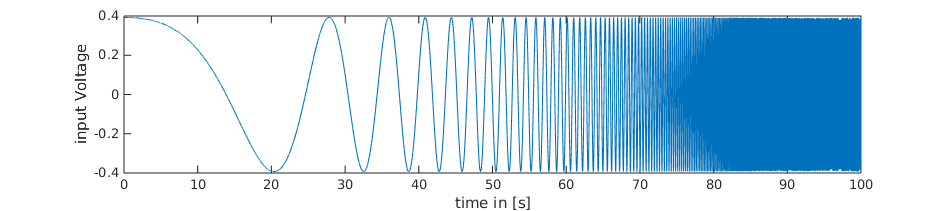
\includegraphics[scale = 0.5]{images/input.png}
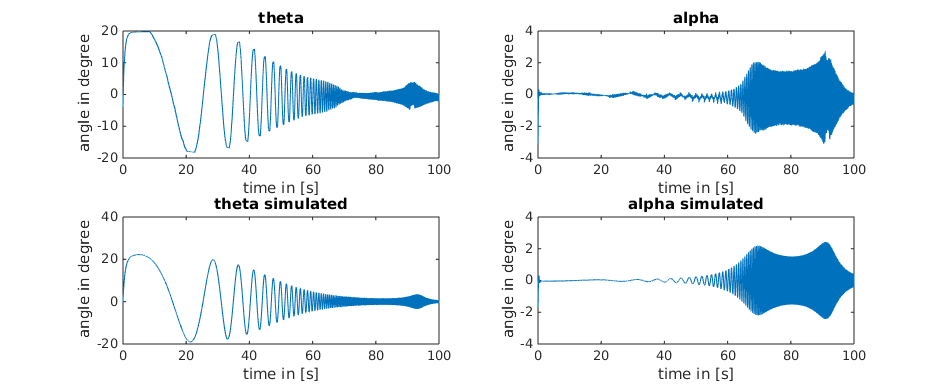
\includegraphics[scale = 0.505]{images/measSim2.png}
\caption{The input signal we used is shown in the top row plot. In the middle row we show the measured plant response to the top input signal. In the bottom the simulated output values are shown. }
\label{fig:timeDomain}
\end{figure}
\begin{figure}
% This file was created by matlab2tikz v0.4.7 running on MATLAB 8.4.
% Copyright (c) 2008--2014, Nico Schlömer <nico.schloemer@gmail.com>
% All rights reserved.
% Minimal pgfplots version: 1.3
% 
% The latest updates can be retrieved from
%   http://www.mathworks.com/matlabcentral/fileexchange/22022-matlab2tikz
% where you can also make suggestions and rate matlab2tikz.
% 
\documentclass[tikz]{standalone}
\usepackage{pgfplots}
\usepackage{grffile}
\pgfplotsset{compat=newest}
\usetikzlibrary{plotmarks}
\usepackage{amsmath}

\begin{document}
%
% defining custom colors
\definecolor{mycolor1}{rgb}{0.00000,0.44700,0.74100}%
\definecolor{mycolor2}{rgb}{0.85000,0.32500,0.09800}%
%
\begin{tikzpicture}

\begin{axis}[%
width=4in,
height=1.5in,
scale only axis,
separate axis lines,
every outer x axis line/.append style={white!40!black},
every x tick label/.append style={font=\color{white!40!black}},
xmode=log,
xmin=0.0001,
xmax=10000,
xtick={0.0001,0.01,1,25,100,10000},
xticklabels={\empty},
xminorticks=true,
every outer y axis line/.append style={white!40!black},
every y tick label/.append style={font=\color{white!40!black}},
ymin=-150,
ymax=50,
ylabel={Magnitude (dB)},
name=plot1,
title={Bode Plot}
]
\addplot [color=mycolor1,solid,forget plot]
  table[row sep=crcr]{1e-20	4.1403119365418\\
9.92127887119004e-15	4.1403119365418\\
9.92127887119004e-11	4.1403119365418\\
9.92127887119002e-08	4.1403119353503\\
9.92127887119002e-06	4.14030002159693\\
9.92127887119002e-05	4.13912075177561\\
0.000115803604796259	4.13868920510392\\
0.000135168812991944	4.13810139235413\\
0.000157772359831077	4.13730079365699\\
0.000184155775105833	4.13621050219696\\
0.000214951145695864	4.13472591816985\\
0.000250896258938453	4.13270486514892\\
0.000292852278342252	4.1299542542419\\
0.000341824375114681	4.12621215454053\\
0.000398985809787651	4.12112380632138\\
0.000465706040882838	4.11420974985489\\
0.000543583534036452	4.10482388186908\\
0.000634484057615856	4.09209899779913\\
0.000740585382304249	4.07487744361978\\
0.000864429455554259	4.05162528363292\\
0.00100898330089217	4.02033057628349\\
0.00117771010108223	3.97839102285847\\
0.00137465216814262	3.92250492015311\\
0.00160452778798681	3.84859365279309\\
0.00187284425986861	3.75180465863165\\
0.00218602983879993	3.62666838561454\\
0.00255158774198283	3.46750152655099\\
0.00297827590890121	3.26914101188767\\
0.00347631682171681	3.02802898821525\\
0.00405764241279103	2.74352641949307\\
0.00473617992676209	2.41913352803303\\
0.00552818558578572	2.06313511502026\\
0.00645263405180261	1.68821390906974\\
0.00753167301646673	1.30987333012784\\
0.00796673513584517	1.17476322884912\\
0.00879115380967962	0.943991826065683\\
0.0102612507389096	0.604232523097061\\
0.011977183997263	0.300099023684295\\
0.0139800634595482	0.036115838959315\\
0.016317873581775	-0.187877037792634\\
0.0190466230000501	-0.375706450706102\\
0.0219173046607446	-0.520138827230517\\
0.0222316863706562	-0.533630463435003\\
0.0259493705987627	-0.669275607978893\\
0.0302887429790625	-0.790936254631337\\
0.035353765046442	-0.907255357480673\\
0.0412657832589166	-1.02721030957809\\
0.0481664361839521	-1.16029260790122\\
0.056221047837773	-1.31676339170586\\
0.065622588474384	-1.5078638079342\\
0.0765962977158366	-1.74585110130552\\
0.0894050807834756	-2.04372787666353\\
0.104355807111643	-2.41455860470728\\
0.121806662244358	-2.87035467559594\\
0.142175729149776	-3.42066611261087\\
0.16595100454127	-4.07119782633763\\
0.193702090173525	-4.82286492727451\\
0.226093839210606	-5.67161424465359\\
0.26390228460208	-6.609073963\\
0.308033231075012	-7.6237912937644\\
0.359543956163856	-8.70265045956224\\
0.419668540185773	-9.83209394894519\\
0.489847432010212	-10.9989294947266\\
0.571761958951658	-12.1906774640725\\
0.667374607564385	-13.395524645703\\
0.778976040375876	-14.6019905637831\\
0.909239974973332	-15.7984071252405\\
0.929375788305583	-15.9663689342942\\
1.06128724022191	-16.9722918893594\\
1.23876054425662	-18.1096792591162\\
1.44591174551961	-19.1944688623333\\
1.68770371765931	-20.2078497102743\\
1.96992924874365	-21.1278411550299\\
2.29934982334327	-21.928919726802\\
2.68385761238917	-22.5815261634342\\
3.13266455171487	-23.0509258373077\\
3.65652303917676	-23.294397412901\\
3.89955851344994	-23.3163632634448\\
4.23848455891898	-23.2638358081471\\
4.88110808451055	-22.9274125994304\\
5.51344196224724	-22.3213290667674\\
6.12457008898291	-21.4875595392423\\
6.70611197619057	-20.4690271892861\\
7.2521388516065	-19.3232802846074\\
7.75892757338603	-18.1430826745573\\
8.22462809324556	-17.0775822490034\\
8.64890212414154	-16.3225902864721\\
9.03257238258247	-16.035002763149\\
9.43326247372579	-16.2884946612887\\
9.91988487766333	-17.2850949652291\\
10.5152887528484	-19.040252301637\\
11.2501105558008	-21.3066129576492\\
12.1661201209076	-23.8160288071619\\
13.3213209517112	-26.4107660998381\\
14.7979001874425	-29.025679716275\\
16.7149266998403	-31.6432018124363\\
19.2491827473828	-34.2654676008695\\
20.0339668073759	-34.9444594865046\\
23.3841383231318	-37.3636568589955\\
27.2945408352199	-39.5176661494014\\
31.8588587319695	-41.4721087553364\\
37.1864427334085	-43.2749994102456\\
43.4049296868704	-44.9626720930345\\
50.6633004567973	-46.5630194118659\\
59.1354491688566	-48.0974984474673\\
69.0243493193747	-49.5825461593154\\
80.5669165606372	-51.0306705354982\\
94.0396846633756	-52.4513237706025\\
109.76543063965	-53.8516040439994\\
128.120907749069	-55.2368137257913\\
149.545871653656	-56.6108969623639\\
174.553615967604	-57.9767778970516\\
203.743269609816	-59.3366189594801\\
237.81415057596	-60.6920162144709\\
277.582520013906	-62.0441460008022\\
324.001137992247	-63.3938743761283\\
378.182089473833	-64.741838449803\\
441.423427352951	-66.0885066296128\\
515.240270862982	-67.4342231421114\\
601.401104401951	-68.77924087321\\
701.970146413631	-70.1237455613505\\
819.356803386633	-71.4678736029929\\
8193.56803386634	-91.4707138920383\\
819356.803386634	-131.47074258187\\
819356803.386633	-191.47074258474\\
8193568033866.33	-271.47074258474\\
8.19356803386633e+17	-371.47074258474\\
1e+20	-413.201281301729\\
};
\addplot [color=mycolor2,solid,forget plot]
  table[row sep=crcr]{1e-20	-54.7105105494891\\
1.22283537208208e-18	-54.7105105494891\\
1.22283537208208e-13	-54.7105105494891\\
1.22283537208208e-09	-54.7105105494891\\
1.22283537208208e-06	-54.7105105477399\\
0.000122283537208208	-54.7104930580007\\
0.00122283537208208	-54.7087617445229\\
0.00142710659710899	-54.7081288497761\\
0.00166550075832718	-54.7072669939641\\
0.00194371799668485	-54.7060934183595\\
0.00226841064571547	-54.7044955123453\\
0.00264734229264307	-54.702320098034\\
0.0030895734101998	-54.6993589133255\\
0.00360567799771882	-54.6953289828315\\
0.00420799641151522	-54.6898461468446\\
0.00491093042987413	-54.6823894933514\\
0.00573128760781893	-54.6722538057799\\
0.00668868315537932	-54.6584864269102\\
0.00780600894849884	-54.6398042332284\\
0.00910998088690125	-54.6144859118387\\
0.010631777686556	-54.580234828516\\
0.0124077863806362	-54.5340091843706\\
0.0144804723543248	-54.4718200560622\\
0.0168993947164984	-54.3885060257058\\
0.0197223912864085	-54.2775075257519\\
0.0230169615290695	-54.1306863421615\\
0.0268618805061309	-53.9382648427688\\
0.0313490824327248	-53.6889878186761\\
0.0365858588772097	-53.3706190640115\\
0.0426974241640272	-52.9708466049595\\
0.0498299093199229	-52.4785603030441\\
0.0581538561505004	-51.8852933539474\\
0.0678682949924807	-51.1864571839171\\
0.0792055036430589	-50.3819624542452\\
0.0924365612550849	-49.4759782841704\\
0.107877829994884	-48.4758770975588\\
0.125898519442867	-47.3906752033994\\
0.146929514606084	-46.2293672647507\\
0.171473678625556	-44.9994569729214\\
0.200117876522019	-43.7058057430137\\
0.233547007474729	-42.3497636677469\\
0.272560381153152	-40.928462967602\\
0.318090829669013	-39.4341407559243\\
0.371227012126413	-37.8533940123507\\
0.433239445084604	-36.1663502323431\\
0.505610881336672	-34.3459134123757\\
0.573772278218495	-32.7324428961458\\
0.590071763378156	-32.3577399727658\\
0.590358538118631	-32.3511811550279\\
0.67344727791234	-30.4943309528639\\
0.756647614730103	-28.7103993220197\\
0.838778351670229	-27.0210666363109\\
0.918835131193553	-25.4594333957602\\
0.996002600996773	-24.0671900591763\\
1.06965272608221	-22.8867896569451\\
1.13933315339817	-21.9488105593693\\
1.21355277538222	-21.1823717482716\\
1.30328980379483	-20.600908822423\\
1.4127453232508	-20.3508875473523\\
1.54758409280284	-20.5096571474865\\
1.71556747046015	-21.0151508258547\\
1.92751545222104	-21.7046070325386\\
2.19879945934039	-22.40727401484\\
2.3697395779853	-22.7313379489042\\
2.76559793933251	-23.2020384413985\\
3.22758333155867	-23.4036486171406\\
3.76674209001964	-23.3321810089677\\
3.8297613255184	-23.3074888664246\\
4.38878870201783	-22.9684136784268\\
4.9431166068772	-22.4513557217149\\
5.48397063013823	-21.80619361692\\
6.00428130768926	-21.0889870958637\\
6.4986966483146	-20.3740978915044\\
6.96347564446679	-19.7585693913015\\
7.39630758009708	-19.3481454592469\\
7.79609409772114	-19.219486423033\\
8.21748994648012	-19.4299158108066\\
8.72826822174898	-20.1665547833129\\
9.35250350488127	-21.5735827129884\\
10.1226241852937	-23.6051125272391\\
11.0830431597316	-26.0839850090187\\
12.2957008734049	-28.8456356062296\\
13.848714829351	-31.8012965389746\\
15.8702013035487	-34.9274345362809\\
17.6542834426043	-37.2147679618239\\
20.6033820605588	-40.3426377791155\\
24.0451193453103	-43.297038009207\\
28.0617892067831	-46.114608282351\\
32.7494325221351	-48.8166317425293\\
38.2201335281441	-51.4135781322421\\
44.6046998195109	-53.9084836035816\\
52.0557900333762	-56.2997020216581\\
60.7515640047787	-58.5834020229427\\
70.8999426703609	-60.7559048152253\\
82.7435795770633	-62.8156923221943\\
96.5656628674247	-64.7647675864932\\
112.696686470282	-66.6091066467054\\
131.522352399917	-68.3581855311997\\
153.492793112152	-70.0238502661941\\
179.133334429202	-71.6189503791663\\
209.057056381002	-73.1561152767645\\
243.979452299887	-74.6468880648799\\
284.735536676016	-76.1012573245602\\
332.29981083213	-77.527515920265\\
387.809563808375	-78.9323368414789\\
452.592065594701	-80.3209647149462\\
528.196302916587	-81.6974495209607\\
616.430016394919	-83.0648778678077\\
719.402924659709	-84.4255792789099\\
839.577168931014	-85.7812992092269\\
979.826184225816	-87.1333385046753\\
1143.50340483521	-88.482662832878\\
1334.52244685918	-89.8299869619488\\
1557.45068500924	-91.1758388163061\\
1817.61846115408	-92.5206077040106\\
2121.24653584684	-93.8645803803091\\
2475.59483027321	-95.2079678824543\\
2889.13601512558	-96.5509254258523\\
3371.75809701239	-97.8935671170739\\
3935.00084636008	-99.2359768131866\\
39350.0084636008	-119.237731047868\\
3935000.84636008	-159.237748769111\\
3935000846.36008	-219.237748770884\\
39350008463600.8	-299.237748770884\\
3.93500084636008e+18	-399.237748770884\\
1e+20	-427.338852168776\\
};
\end{axis}

\begin{axis}[%
width=4in,
height=1in,
scale only axis,
separate axis lines,
every outer x axis line/.append style={white!40!black},
every x tick label/.append style={font=\color{white!40!black}},
xmode=log,
xmin=0.0001,
xmax=10000,
xminorticks=true,
every outer y axis line/.append style={white!40!black},
every y tick label/.append style={font=\color{white!40!black}},
ymin=-94.5,
ymax=364.5,
ytick={-90,   0,  90, 180, 270, 360},
ylabel={Phase (deg)},
at=(plot1.below south west),
anchor=above north west
]
\addplot [color=mycolor1,solid,forget plot]
  table[row sep=crcr]{1e-20	360\\
9.92127887119004e-15	359.999999999946\\
9.92127887119004e-11	359.999999462542\\
9.92127887119002e-08	359.9994625424\\
9.92127887119002e-06	359.946254365716\\
9.92127887119002e-05	359.462668133794\\
0.000115803604796259	359.372866210575\\
0.000135168812991944	359.268078561233\\
0.000157772359831077	359.145817692101\\
0.000184155775105833	359.003191024786\\
0.000214951145695864	358.836839549551\\
0.000250896258938453	358.642869957187\\
0.000292852278342252	358.416781322256\\
0.000341824375114681	358.153388818035\\
0.000398985809787651	357.846749255235\\
0.000465706040882838	357.490096935152\\
0.000543583534036452	357.075804082653\\
0.000634484057615856	356.595388905017\\
0.000740585382304249	356.039607246238\\
0.000864429455554259	355.398681998697\\
0.00100898330089217	354.662748374193\\
0.00117771010108223	353.822621201878\\
0.00137465216814262	352.871016050907\\
0.00160452778798681	351.804363012258\\
0.00187284425986861	350.625308865746\\
0.00218602983879993	349.34586033802\\
0.00255158774198283	347.990821227981\\
0.00297827590890121	346.600697683728\\
0.00347631682171681	345.232687342544\\
0.00405764241279103	343.958038505088\\
0.00473617992676209	342.854455642371\\
0.00552818558578572	341.993705522556\\
0.00645263405180261	341.42687236741\\
0.00753167301646673	341.171663888018\\
0.00796673513584517	341.153090557733\\
0.00879115380967962	341.206322018663\\
0.0102612507389096	341.472475691897\\
0.011977183997263	341.885728316956\\
0.0139800634595482	342.349925215727\\
0.016317873581775	342.770400741694\\
0.0190466230000501	343.063010215006\\
0.0219173046607446	343.15917398263\\
0.0222316863706562	343.158110472556\\
0.0259493705987627	343.000497983004\\
0.0302887429790625	342.54707408135\\
0.035353765046442	341.763896331573\\
0.0412657832589166	340.62378995812\\
0.0481664361839521	339.105207703023\\
0.056221047837773	337.192678198366\\
0.065622588474384	334.87893652491\\
0.0765962977158366	332.168572946897\\
0.0894050807834756	329.08265592599\\
0.104355807111643	325.663256099669\\
0.121806662244358	321.976268051017\\
0.142175729149776	318.110760531734\\
0.16595100454127	314.173707164736\\
0.193702090173525	310.280445345663\\
0.226093839210606	306.542986615186\\
0.26390228460208	303.059304541565\\
0.308033231075012	299.906272664251\\
0.359543956163856	297.137332370886\\
0.419668540185773	294.784256960706\\
0.489847432010212	292.861389028356\\
0.571761958951658	291.370625938744\\
0.667374607564385	290.305863511946\\
0.778976040375876	289.656152398781\\
0.909239974973332	289.407224389343\\
0.929375788305583	289.403396719573\\
1.06128724022191	289.541253508115\\
1.23876054425662	290.034790242217\\
1.44591174551961	290.854848383352\\
1.68770371765931	291.953232501136\\
1.96992924874365	293.259426437205\\
2.29934982334327	294.672652541605\\
2.68385761238917	296.053733422207\\
3.13266455171487	297.216401991695\\
3.65652303917676	297.914339833715\\
3.89955851344994	297.992569210104\\
4.23848455891898	297.839486141324\\
4.88110808451055	296.688140940469\\
5.51344196224724	294.357466913286\\
6.12457008898291	290.74131528753\\
6.70611197619057	285.643433560336\\
7.2521388516065	278.761010189502\\
7.75892757338603	269.734471830875\\
8.22462809324556	258.351058181198\\
8.64890212414154	244.956471711624\\
9.03257238258247	230.771336917874\\
9.43326247372579	215.344233719033\\
9.91988487766333	198.42192233054\\
10.5152887528484	182.579417331933\\
11.2501105558008	169.459173906649\\
12.1661201209076	159.131031819143\\
13.3213209517112	150.915805638711\\
14.7979001874425	144.070950170258\\
16.7149266998403	138.009092714408\\
19.2491827473828	132.316801132688\\
20.0339668073759	130.872198825941\\
23.3841383231318	125.767859376744\\
27.2945408352199	121.268662928466\\
31.8588587319695	117.262247494999\\
37.1864427334085	113.695762598154\\
43.4049296868704	110.535510908772\\
50.6633004567973	107.751554237989\\
59.1354491688566	105.312971200383\\
69.0243493193747	103.187444145925\\
80.5669165606372	101.342285981449\\
94.0396846633756	99.7456578761044\\
109.76543063965	98.367522655558\\
128.120907749069	97.1802389777824\\
149.545871653656	96.158842524734\\
174.553615967604	95.2810986335173\\
203.743269609816	94.5274065418265\\
237.81415057596	93.8806177992838\\
277.582520013906	93.3258127985999\\
324.001137992247	92.8500641044349\\
378.182089473833	92.4422040625597\\
441.423427352951	92.0926065126246\\
515.240270862982	91.7929874449596\\
601.401104401951	91.5362263415939\\
701.970146413631	91.3162081043945\\
819.356803386633	91.1276844536597\\
8193.56803386634	90.1127808307605\\
819356.803386634	90.0011278095589\\
819356803.386633	90.0000011278095\\
8193568033866.33	90.0000000001128\\
8.19356803386633e+17	90\\
1e+20	90\\
};
\addplot [color=mycolor2,solid,forget plot]
  table[row sep=crcr]{1e-20	180\\
1.22283537208208e-18	180\\
1.22283537208208e-13	180.000000000117\\
1.22283537208208e-09	180.000001171255\\
1.22283537208208e-06	180.001171254858\\
0.000122283537208208	180.117125332959\\
0.00122283537208208	181.171102047559\\
0.00142710659710899	181.36666682879\\
0.00166550075832718	181.594862134633\\
0.00194371799668485	181.861116411223\\
0.00226841064571547	182.171751739641\\
0.00264734229264307	182.534125383238\\
0.0030895734101998	182.956790460354\\
0.00360567799771882	183.449676317338\\
0.00420799641151522	184.024287779483\\
0.00491093042987413	184.693920005227\\
0.00573128760781893	185.473881567194\\
0.00668868315537932	186.38171176575\\
0.00780600894849884	187.4373678381\\
0.00910998088690125	188.663342091227\\
0.010631777686556	190.084646282447\\
0.0124077863806362	191.728569356314\\
0.0144804723543248	193.62407518138\\
0.0168993947164984	195.800663972182\\
0.0197223912864085	198.286488691852\\
0.0230169615290695	201.105525715814\\
0.0268618805061309	204.273697513695\\
0.0313490824327248	207.794097258737\\
0.0365858588772097	211.651911260456\\
0.0426974241640272	215.810215326471\\
0.0498299093199229	220.208288696565\\
0.0581538561505004	224.764021664577\\
0.0678682949924807	229.381040469638\\
0.0792055036430589	233.959483650816\\
0.0924365612550849	238.407764203324\\
0.107877829994884	242.652155095292\\
0.125898519442867	246.641975918281\\
0.146929514606084	250.349872093098\\
0.171473678625556	253.768111702544\\
0.200117876522019	256.902359777692\\
0.233547007474729	259.764077926051\\
0.272560381153152	262.361925112222\\
0.318090829669013	264.691616674036\\
0.371227012126413	266.722684509948\\
0.433239445084604	268.379218717544\\
0.505610881336672	269.50929933894\\
0.573772278218495	269.852798140538\\
0.590071763378156	269.833044058082\\
0.590358538118631	269.832341950524\\
0.67344727791234	269.100648738901\\
0.756647614730103	267.25213423621\\
0.838778351670229	264.212996023157\\
0.918835131193553	259.962884779128\\
0.996002600996773	254.578696983262\\
1.06965272608221	248.273799761864\\
1.13933315339817	241.401606949801\\
1.21355277538222	233.431108706708\\
1.30328980379483	223.568513424947\\
1.4127453232508	212.352060313065\\
1.54758409280284	200.988916586073\\
1.71556747046015	190.79095574416\\
1.92751545222104	182.465445053396\\
2.19879945934039	175.981008857621\\
2.3697395779853	173.194296796814\\
2.76559793933251	168.608119202124\\
3.22758333155867	164.711923271351\\
3.76674209001964	160.70924399879\\
3.8297613255184	160.242626860124\\
4.38878870201783	155.898967500143\\
4.9431166068772	150.928977152356\\
5.48397063013823	145.038880087301\\
6.00428130768926	137.967986240564\\
6.4986966483146	129.520402033619\\
6.96347564446679	119.674583954107\\
7.39630758009708	108.733768377466\\
7.79609409772114	97.3795915469377\\
8.21748994648012	84.8501864205824\\
8.72826822174898	70.321803456444\\
9.35250350488127	55.3288396380165\\
10.1226241852937	41.6372030039926\\
11.0830431597316	30.1722006153584\\
12.2957008734049	20.9004989891189\\
13.848714829351	13.3350457912141\\
15.8702013035487	6.91416434623856\\
17.6542834426043	2.8422561932743\\
20.6033820605588	-2.24696893943547\\
24.0451193453103	-6.82847363669036\\
28.0617892067831	-11.2029207114516\\
32.7494325221351	-15.5482615016352\\
38.2201335281441	-19.9700063656432\\
44.6046998195109	-24.5228696318639\\
52.0557900333762	-29.220017388445\\
60.7515640047787	-34.0379683398425\\
70.8999426703609	-38.9218480287032\\
82.7435795770633	-43.79354374652\\
96.5656628674247	-48.5631078567259\\
112.696686470282	-53.1416590506552\\
131.522352399917	-57.4528880024529\\
153.492793112152	-61.4406592494269\\
179.133334429202	-65.0717377398581\\
209.057056381002	-68.3343210308758\\
243.979452299887	-71.2339887330393\\
284.735536676016	-73.7887350673341\\
332.29981083213	-76.0242747349046\\
387.809563808375	-77.9702270498122\\
452.592065594701	-79.6573341421081\\
528.196302916587	-81.115614890419\\
616.430016394919	-82.3732564920336\\
719.402924659709	-83.4560367708388\\
839.577168931014	-84.3871021759772\\
979.826184225816	-85.186969026051\\
1143.50340483521	-85.8736547789557\\
1334.52244685918	-86.4628771576025\\
1557.45068500924	-86.9682815506717\\
1817.61846115408	-87.4016726591961\\
2121.24653584684	-87.7732366413178\\
2475.59483027321	-88.0917465794589\\
2889.13601512558	-88.3647481604315\\
3371.75809701239	-88.5987248834408\\
3935.00084636008	-88.799243485855\\
39350.0084636008	-89.8799092498077\\
3935000.84636008	-89.9987990909728\\
3935000846.36008	-89.999998799091\\
39350008463600.8	-89.9999999998799\\
3.93500084636008e+18	-90\\
1e+20	-90\\
};
\end{axis}
\end{tikzpicture}%
\end{document}
%% This file was created by matlab2tikz v0.4.7 running on MATLAB 8.4.
% Copyright (c) 2008--2014, Nico Schlömer <nico.schloemer@gmail.com>
% All rights reserved.
% Minimal pgfplots version: 1.3
% 
% The latest updates can be retrieved from
%   http://www.mathworks.com/matlabcentral/fileexchange/22022-matlab2tikz
% where you can also make suggestions and rate matlab2tikz.
% 
\documentclass[tikz]{standalone}
\usepackage{pgfplots}
\usepackage{grffile}
\pgfplotsset{compat=newest}
\usetikzlibrary{plotmarks}
\usepackage{amsmath}

\begin{document}
%
% defining custom colors
\definecolor{mycolor1}{rgb}{0.00000,0.44700,0.74100}%
\definecolor{mycolor2}{rgb}{0.85000,0.32500,0.09800}%
%
\begin{tikzpicture}

\begin{axis}[%
width=4.52083333333333in,
height=3.565625in,
scale only axis,
separate axis lines,
every outer x axis line/.append style={white!15!black},
every x tick label/.append style={font=\color{white!15!black}},
xmin=0,
xmax=100,
every outer y axis line/.append style={white!15!black},
every y tick label/.append style={font=\color{white!15!black}},
ymin=-10,
ymax=15
]
\addplot [color=mycolor1,solid,forget plot]
  table[row sep=crcr]{0	0\\
0.005	-0.0236136012441993\\
0.01	-0.0451910095868532\\
0.015	-0.0646834704058247\\
0.02	-0.0820474461769308\\
0.025	-0.0972446312163101\\
0.03	-0.110241955012036\\
0.035	-0.121011574309225\\
0.04	-0.12953085413448\\
0.045	-0.135782337966365\\
0.05	-0.139753707278725\\
0.055	-0.141437730702988\\
0.06	-0.140832203074074\\
0.065	-0.137939874642223\\
0.07	-0.132768370749827\\
0.075	-0.125330102288257\\
0.08	-0.115642167264673\\
0.085	-0.103726243822841\\
0.09	-0.0896084750751191\\
0.095	-0.0733193461148953\\
0.1	-0.054893553589967\\
0.105	-0.034369868227518\\
0.11	-0.0117909907105784\\
0.115	0.0127965986859438\\
0.12	0.0393427962843529\\
0.125	0.0677940365968471\\
0.13	0.0980934588950368\\
0.135	0.130181078325312\\
0.14	0.16399396113582\\
0.145	0.199466403578538\\
0.15	0.236530114048638\\
0.155	0.275114398022969\\
0.16	0.315146345360095\\
0.165	0.356551019525837\\
0.17	0.399251648310715\\
0.175	0.443169815608975\\
0.18	0.488225653833115\\
0.185	0.534338036542846\\
0.19	0.581424770873278\\
0.195	0.62940278935382\\
0.2	0.678188340716679\\
0.205	0.72769717930207\\
0.21	0.777844752676118\\
0.215	0.82854638708704\\
0.22	0.879717470395434\\
0.225	0.931273632125393\\
0.23	0.983130920294581\\
0.235	1.03520597469349\\
0.24	1.08741619629659\\
0.245	1.13967991250118\\
0.25	1.19191653790314\\
0.255	1.24404673033284\\
0.26	1.29599254188865\\
0.265	1.34767756472011\\
0.27	1.39902707132796\\
0.275	1.44996814916313\\
0.28	1.50042982932264\\
0.285	1.55034320915571\\
0.29	1.59964156860932\\
0.295	1.64826048015847\\
0.3	1.6961379121824\\
0.305	1.74321432566398\\
0.31	1.78943276410591\\
0.315	1.83473893657321\\
0.32	1.87908129378758\\
0.325	1.92241109721537\\
0.33	1.96468248110655\\
0.335	2.00585250745784\\
0.34	2.0458812138888\\
0.345	2.08473165443482\\
0.35	2.12236993327633\\
0.355	2.15876523143788\\
0.36	2.19388982650596\\
0.365	2.22771910542783\\
0.37	2.2602315704683\\
0.375	2.29140883841414\\
0.38	2.32123563312943\\
0.385	2.34969977157763\\
0.39	2.37679214343825\\
0.395	2.40250668445808\\
0.4	2.426840343688\\
0.405	2.44979304476717\\
0.41	2.47136764142706\\
0.415	2.49156986739703\\
0.42	2.5104082809028\\
0.425	2.52789420395775\\
0.43	2.54404165665504\\
0.435	2.55886728667613\\
0.44	2.57239029423844\\
0.445	2.58463235271095\\
0.45	2.59561752513282\\
0.455	2.60537217687494\\
0.46	2.61392488468912\\
0.465	2.62130634239388\\
0.47	2.62754926344882\\
0.475	2.63268828067281\\
0.48	2.63675984336337\\
0.485	2.63980211207623\\
0.49	2.64185485132529\\
0.495	2.64295932046372\\
0.5	2.64315816300682\\
0.505	2.64249529465685\\
0.51	2.6410157902887\\
0.515	2.63876577015375\\
0.52	2.63579228555712\\
0.525	2.63214320426055\\
0.53	2.62786709586029\\
0.535	2.62301311738546\\
0.54	2.61763089935813\\
0.545	2.61177043255208\\
0.55	2.60548195568174\\
0.555	2.5988158442477\\
0.56	2.59182250075898\\
0.565	2.58455224654632\\
0.57	2.57705521537389\\
0.575	2.56938124904996\\
0.58	2.56157979522974\\
0.585	2.55369980759614\\
0.59	2.54578964859601\\
0.595	2.53789699490181\\
0.6	2.53006874575959\\
0.605	2.52235093437631\\
0.61	2.51478864249013\\
0.615	2.50742591825862\\
0.62	2.50030569759078\\
0.625	2.49346972903923\\
0.63	2.48695850235992\\
0.635	2.48081118083682\\
0.64	2.47506553746013\\
0.645	2.46975789503621\\
0.65	2.46492307029867\\
0.655	2.46059432207977\\
0.66	2.4568033035921\\
0.665	2.45358001886096\\
0.67	2.45095278333806\\
0.675	2.44894818871814\\
0.68	2.44759107197067\\
0.685	2.44690448858934\\
0.69	2.4469096900535\\
0.695	2.44762610548618\\
0.7	2.44907132748519\\
0.705	2.45126110209471\\
0.71	2.45420932287671\\
0.715	2.45792802903338\\
0.72	2.46242740752355\\
0.725	2.46771579910883\\
0.73	2.47379970825731\\
0.735	2.48068381682581\\
0.74	2.48837100143473\\
0.745	2.49686235444265\\
0.75	2.50615720842204\\
0.755	2.51625316403095\\
0.76	2.52714612117018\\
0.765	2.53883031330986\\
0.77	2.55129834486449\\
0.775	2.56454123149073\\
0.78	2.57854844317781\\
0.785	2.59330794999644\\
0.79	2.60880627036857\\
0.795	2.62502852171678\\
0.8	2.64195847334928\\
0.805	2.65957860143386\\
0.81	2.67787014591181\\
0.815	2.69681316920095\\
0.82	2.71638661653544\\
0.825	2.73656837778857\\
0.83	2.7573353506242\\
0.835	2.77866350482171\\
0.84	2.8005279476194\\
0.845	2.82290298992115\\
0.85	2.84576221321181\\
0.855	2.86907853702771\\
0.86	2.89282428682943\\
0.865	2.91697126212577\\
0.87	2.94149080469943\\
0.875	2.96635386678696\\
0.88	2.99153107906776\\
0.885	3.01699281831978\\
0.89	3.04270927460199\\
0.895	3.06865051782728\\
0.9	3.09478656359234\\
0.905	3.12108743813515\\
0.91	3.14752324229395\\
0.915	3.17406421434617\\
0.92	3.20068079160959\\
0.925	3.22734367069263\\
0.93	3.25402386628516\\
0.935	3.28069276838612\\
0.94	3.30732219786884\\
0.945	3.33388446029043\\
0.95	3.36035239785629\\
0.955	3.38669943945653\\
0.96	3.41289964869606\\
0.965	3.43892776984587\\
0.97	3.46475927164845\\
0.975	3.49037038891578\\
0.98	3.51573816186425\\
0.985	3.54084047313618\\
0.99	3.5656560824637\\
0.995	3.59016465893609\\
1	3.61434681083768\\
1.005	3.63818411302893\\
1.01	3.66165913184906\\
1.015	3.68475544752415\\
1.02	3.70745767407029\\
1.025	3.72975147668684\\
1.03	3.75162358664021\\
1.035	3.7730618136442\\
1.04	3.7940550557478\\
1.045	3.81459330674687\\
1.05	3.83466766114106\\
1.055	3.85427031666214\\
1.06	3.87339457440486\\
1.065	3.89203483659607\\
1.07	3.91018660204232\\
1.075	3.92784645930062\\
1.08	3.94501207762098\\
1.085	3.96168219571379\\
1.09	3.97785660839858\\
1.095	3.99353615119459\\
1.1	4.00872268291699\\
1.105	4.02341906634596\\
1.11	4.0376291470389\\
1.115	4.05135773035895\\
1.12	4.06461055679581\\
1.125	4.07739427565713\\
1.13	4.08971641721145\\
1.135	4.10158536336532\\
1.14	4.11301031695935\\
1.145	4.12400126976977\\
1.15	4.13456896930314\\
1.155	4.14472488447354\\
1.16	4.15448117025231\\
1.165	4.16385063138144\\
1.17	4.17284668524224\\
1.175	4.18148332397149\\
1.18	4.18977507591715\\
1.185	4.19773696652635\\
1.19	4.20538447875746\\
1.195	4.21273351310833\\
1.2	4.21980034735183\\
1.205	4.22660159606917\\
1.21	4.23315417007073\\
1.215	4.23947523579265\\
1.22	4.24558217475667\\
1.225	4.25149254317866\\
1.23	4.25722403181027\\
1.235	4.26279442609589\\
1.24	4.2682215667255\\
1.245	4.27352331066179\\
1.25	4.27871749271781\\
1.255	4.283821887759\\
1.26	4.28885417360116\\
1.265	4.29383189467309\\
1.27	4.29877242651033\\
1.275	4.30369294114336\\
1.28	4.30861037344074\\
1.285	4.31354138846508\\
1.29	4.31850234989622\\
1.295	4.32350928957323\\
1.3	4.32857787820357\\
1.305	4.33372339728446\\
1.31	4.33896071227839\\
1.315	4.34430424708124\\
1.32	4.34976795981823\\
1.325	4.35536531999951\\
1.33	4.36110928706386\\
1.335	4.36701229033546\\
1.34	4.37308621041551\\
1.345	4.3793423620268\\
1.35	4.38579147832618\\
1.355	4.39244369669645\\
1.36	4.39930854602579\\
1.365	4.40639493547956\\
1.37	4.41371114476626\\
1.375	4.42126481589574\\
1.38	4.42906294642511\\
1.385	4.43711188418435\\
1.39	4.44541732347069\\
1.395	4.45398430269788\\
1.4	4.4628172034834\\
1.405	4.47191975115414\\
1.41	4.48129501664809\\
1.415	4.49094541978691\\
1.42	4.50087273389199\\
1.425	4.51107809171372\\
1.43	4.52156199264183\\
1.435	4.53232431116185\\
1.44	4.54336430652114\\
1.445	4.55468063356549\\
1.45	4.56627135470562\\
1.455	4.57813395297093\\
1.46	4.59026534610641\\
1.465	4.60266190166668\\
1.47	4.6153194530601\\
1.475	4.6282333164942\\
1.48	4.64139830877285\\
1.485	4.65480876589406\\
1.49	4.66845856239688\\
1.495	4.68234113140454\\
1.5	4.69644948531067\\
1.505	4.71077623705461\\
1.51	4.72531362193151\\
1.515	4.7400535198825\\
1.52	4.75498747821008\\
1.525	4.77010673466375\\
1.53	4.78540224084098\\
1.535	4.80086468584863\\
1.54	4.81648452017044\\
1.545	4.8322519796864\\
1.55	4.84815710979026\\
1.555	4.86418978955229\\
1.56	4.88033975587479\\
1.565	4.89659662758884\\
1.57	4.91294992944173\\
1.575	4.92938911592524\\
1.58	4.94590359489635\\
1.585	4.96248275094284\\
1.59	4.97911596844786\\
1.595	4.99579265430834\\
1.6	5.01250226026418\\
1.605	5.02923430479606\\
1.61	5.04597839455172\\
1.615	5.06272424526172\\
1.62	5.07946170210793\\
1.625	5.09618075950907\\
1.63	5.11287158029004\\
1.635	5.12952451420309\\
1.64	5.14613011577105\\
1.645	5.16267916142458\\
1.65	5.17916266590753\\
1.655	5.19557189792607\\
1.66	5.21189839501975\\
1.665	5.22813397763416\\
1.67	5.24427076237726\\
1.675	5.26030117444303\\
1.68	5.27621795918879\\
1.685	5.29201419285362\\
1.69	5.30768329240837\\
1.695	5.3232190245288\\
1.7	5.3386155136862\\
1.705	5.3538672493511\\
1.71	5.36896909230826\\
1.715	5.38391628008266\\
1.72	5.39870443147817\\
1.725	5.4133295502327\\
1.73	5.42778802779508\\
1.735	5.44207664523114\\
1.74	5.45619257426773\\
1.745	5.47013337748566\\
1.75	5.48389700767376\\
1.755	5.49748180635803\\
1.76	5.51088650152162\\
1.765	5.52411020453232\\
1.77	5.53715240629644\\
1.775	5.55001297265857\\
1.78	5.56269213906858\\
1.785	5.57519050453828\\
1.79	5.58750902491118\\
1.795	5.59964900547022\\
1.8	5.61161209290916\\
1.805	5.62340026669434\\
1.81	5.63501582984448\\
1.815	5.64646139915691\\
1.82	5.65773989490959\\
1.825	5.66885453006862\\
1.83	5.67980879903191\\
1.835	5.69060646594\\
1.84	5.7012515525855\\
1.845	5.71174832595307\\
1.85	5.72210128542211\\
1.855	5.73231514966463\\
1.86	5.7423948432709\\
1.865	5.75234548313554\\
1.87	5.76217236463671\\
1.875	5.77188094764127\\
1.88	5.78147684236824\\
1.885	5.79096579514294\\
1.89	5.80035367407413\\
1.895	5.80964645468568\\
1.9	5.81885020553428\\
1.905	5.82797107384428\\
1.91	5.83701527118992\\
1.915	5.84598905925494\\
1.92	5.85489873569901\\
1.925	5.86375062015934\\
1.93	5.87255104041555\\
1.935	5.88130631874494\\
1.94	5.8900227584944\\
1.945	5.89870663089447\\
1.95	5.90736416214014\\
1.955	5.91600152076195\\
1.96	5.92462480531008\\
1.965	5.93324003237308\\
1.97	5.94185312495184\\
1.975	5.95046990120823\\
1.98	5.95909606360703\\
1.985	5.96773718846831\\
1.99	5.97639871594648\\
1.995	5.98508594045107\\
2	5.99380400152311\\
2.005	6.00255787517962\\
2.01	6.01135236573797\\
2.015	6.02019209813008\\
2.02	6.02908151071579\\
2.025	6.03802484860314\\
2.03	6.04702615748227\\
2.035	6.05608927797837\\
2.04	6.06521784052809\\
2.045	6.07441526078232\\
2.05	6.08368473553745\\
2.055	6.0930292391957\\
2.06	6.10245152075431\\
2.065	6.111954101322\\
2.07	6.12153927216002\\
2.075	6.13120909324431\\
2.08	6.14096539234378\\
2.085	6.15080976460912\\
2.09	6.16074357266521\\
2.095	6.1707679471995\\
2.1	6.1808837880375\\
2.105	6.19109176569595\\
2.11	6.20139232340298\\
2.115	6.21178567957407\\
2.12	6.22227183073163\\
2.125	6.23285055485519\\
2.13	6.24352141514882\\
2.135	6.25428376421112\\
2.14	6.2651367485931\\
2.145	6.27607931372828\\
2.15	6.28711020921873\\
2.155	6.29822799446071\\
2.16	6.30943104459247\\
2.165	6.32071755674681\\
2.17	6.33208555659049\\
2.175	6.34353290513199\\
2.18	6.35505730577931\\
2.185	6.36665631162875\\
2.19	6.37832733296564\\
2.195	6.39006764495793\\
2.2	6.4018743955231\\
2.205	6.41374461334914\\
2.21	6.42567521604994\\
2.215	6.43766301843589\\
2.22	6.44970474087994\\
2.225	6.46179701776012\\
2.23	6.47393640595908\\
2.235	6.48611939340175\\
2.24	6.49834240761218\\
2.245	6.51060182427113\\
2.25	6.52289397575588\\
2.255	6.53521515964451\\
2.26	6.54756164716674\\
2.265	6.55992969158427\\
2.27	6.57231553648366\\
2.275	6.5847154239653\\
2.28	6.59712560271263\\
2.285	6.60954233592595\\
2.29	6.62196190910618\\
2.295	6.63438063767386\\
2.3	6.64679487440979\\
2.305	6.65920101670403\\
2.31	6.67159551360052\\
2.315	6.68397487262552\\
2.32	6.69633566638829\\
2.325	6.70867453894353\\
2.33	6.72098821190538\\
2.335	6.73327349030378\\
2.34	6.74552726817433\\
2.345	6.75774653387398\\
2.35	6.76992837511503\\
2.355	6.7820699837111\\
2.36	6.79416866002908\\
2.365	6.80622181714212\\
2.37	6.81822698467915\\
2.375	6.83018181236728\\
2.38	6.84208407326419\\
2.385	6.8539316666781\\
2.39	6.86572262077395\\
2.395	6.87745509486475\\
2.4	6.88912738138811\\
2.405	6.90073790756832\\
2.41	6.91228523676509\\
2.415	6.92376806951105\\
2.42	6.93518524424013\\
2.425	6.94653573771014\\
2.43	6.9578186651231\\
2.435	6.96903327994769\\
2.44	6.98017897344866\\
2.445	6.99125527392854\\
2.45	7.00226184568768\\
2.455	7.01319848770903\\
2.46	7.02406513207459\\
2.465	7.034861842121\\
2.47	7.04558881034209\\
2.475	7.05624635604668\\
2.48	7.06683492278035\\
2.485	7.07735507552016\\
2.49	7.08780749765188\\
2.495	7.09819298773924\\
2.5	7.10851245609545\\
2.505	7.11876692116716\\
2.51	7.12895750574147\\
2.515	7.1390854329867\\
2.52	7.14915202233798\\
2.525	7.15915868523872\\
2.53	7.16910692074917\\
2.535	7.17899831103366\\
2.54	7.18883451673775\\
2.545	7.19861727226707\\
2.55	7.20834838097916\\
2.555	7.21802971030018\\
2.56	7.22766318677781\\
2.565	7.23725079108209\\
2.57	7.24679455296546\\
2.575	7.25629654619369\\
2.58	7.26575888345857\\
2.585	7.27518371128391\\
2.59	7.28457320493564\\
2.595	7.29392956334681\\
2.6	7.30325500406824\\
2.605	7.31255175825516\\
2.61	7.32182206570004\\
2.615	7.33106816992149\\
2.62	7.34029231331903\\
2.625	7.34949673240291\\
2.63	7.3586836531082\\
2.635	7.3678552862019\\
2.64	7.37701382279135\\
2.645	7.38616142994228\\
2.65	7.39530024641392\\
2.655	7.4044323785188\\
2.66	7.41355989611406\\
2.665	7.42268482873095\\
2.67	7.43180916184867\\
2.675	7.44093483331838\\
2.68	7.45006372994277\\
2.685	7.45919768421617\\
2.69	7.46833847122971\\
2.695	7.47748780574582\\
2.7	7.48664733944556\\
2.705	7.49581865835226\\
2.71	7.50500328043428\\
2.715	7.51420265338922\\
2.72	7.5234181526118\\
2.725	7.53265107934679\\
2.73	7.54190265902831\\
2.735	7.55117403980612\\
2.74	7.56046629125947\\
2.745	7.56978040329807\\
2.75	7.57911728525018\\
2.755	7.58847776513652\\
2.76	7.59786258912911\\
2.765	7.6072724211932\\
2.77	7.61670784291037\\
2.775	7.62616935348055\\
2.78	7.6356573699001\\
2.785	7.64517222731303\\
2.79	7.65471417953205\\
2.795	7.66428339972564\\
2.8	7.67387998126732\\
2.805	7.68350393874278\\
2.81	7.69315520911042\\
2.815	7.70283365301037\\
2.82	7.71253905621718\\
2.825	7.72227113123074\\
2.83	7.73202951899997\\
2.835	7.74181379077369\\
2.84	7.75162345007271\\
2.845	7.76145793477721\\
2.85	7.77131661932302\\
2.855	7.78119881700071\\
2.86	7.79110378235082\\
2.865	7.80103071364883\\
2.87	7.81097875547306\\
2.875	7.82094700134889\\
2.88	7.83093449646237\\
2.885	7.84094024043655\\
2.89	7.85096319016344\\
2.895	7.86100226268489\\
2.9	7.87105633811533\\
2.905	7.88112426259973\\
2.91	7.89120485129958\\
2.915	7.90129689140043\\
2.92	7.911399145134\\
2.925	7.92151035280829\\
2.93	7.93162923583904\\
2.935	7.94175449977606\\
2.94	7.95188483731802\\
2.945	7.96201893130946\\
2.95	7.97215545771381\\
2.955	7.9822930885565\\
2.96	7.99243049483224\\
2.965	8.00256634937087\\
2.97	8.01269932965621\\
2.975	8.02282812059256\\
2.98	8.0329514172139\\
2.985	8.04306792733056\\
2.99	8.05317637410891\\
2.995	8.06327549857943\\
3	8.07336406206887\\
3.005	8.08344084855248\\
3.01	8.09350466692247\\
3.015	8.10355435316907\\
3.02	8.11358877247086\\
3.025	8.12360682119135\\
3.03	8.13360742877872\\
3.035	8.14358955956643\\
3.04	8.153552214472\\
3.045	8.16349443259213\\
3.05	8.17341529269216\\
3.055	8.18331391458833\\
3.06	8.1931894604214\\
3.065	8.2030411358207\\
3.07	8.21286819095766\\
3.075	8.22266992148816\\
3.08	8.23244566938353\\
3.085	8.24219482364997\\
3.09	8.25191682093655\\
3.095	8.26161114603216\\
3.1	8.27127733225209\\
3.105	8.28091496171492\\
3.11	8.2905236655109\\
3.115	8.30010312376312\\
3.12	8.30965306558274\\
3.125	8.31917326892024\\
3.13	8.32866356031438\\
3.135	8.338123814541\\
3.14	8.34755395416393\\
3.145	8.35695394899041\\
3.15	8.36632381543368\\
3.155	8.37566361578541\\
3.16	8.38497345740092\\
3.165	8.3942534918003\\
3.17	8.40350391368849\\
3.175	8.4127249598978\\
3.18	8.42191690825608\\
3.185	8.43108007638429\\
3.19	8.44021482042699\\
3.195	8.4493215337195\\
3.2	8.45840064539546\\
3.205	8.46745261893886\\
3.21	8.47647795068418\\
3.215	8.48547716826891\\
3.22	8.49445082904232\\
3.225	8.5033995184345\\
3.23	8.51232384828996\\
3.235	8.52122445516961\\
3.24	8.53010199862547\\
3.245	8.53895715945207\\
3.25	8.54779063791868\\
3.255	8.55660315198636\\
3.26	8.5653954355141\\
3.265	8.57416823645767\\
3.27	8.58292231506556\\
3.275	8.59165844207559\\
3.28	8.60037739691619\\
3.285	8.60907996591611\\
3.29	8.61776694052624\\
3.295	8.62643911555717\\
3.3	8.63509728743599\\
3.305	8.64374225248586\\
3.31	8.65237480523162\\
3.315	8.66099573673458\\
3.32	8.66960583295989\\
3.325	8.67820587317915\\
3.33	8.68679662841142\\
3.335	8.69537885990524\\
3.34	8.70395331766434\\
3.345	8.71252073901954\\
3.35	8.72108184724915\\
3.355	8.72963735025017\\
3.36	8.73818793926234\\
3.365	8.74673428764694\\
3.37	8.75527704972212\\
3.375	8.76381685965657\\
3.38	8.77235433042269\\
3.385	8.78089005281098\\
3.39	8.78942459450656\\
3.395	8.79795849922901\\
3.4	8.80649228593634\\
3.405	8.81502644809388\\
3.41	8.82356145300865\\
3.415	8.83209774122968\\
3.42	8.8406357260145\\
3.425	8.84917579286208\\
3.43	8.85771829911205\\
3.435	8.86626357361024\\
3.44	8.87481191644008\\
3.445	8.8833635987196\\
3.45	8.89191886246342\\
3.455	8.90047792050901\\
3.46	8.90904095650642\\
3.465	8.91760812497066\\
3.47	8.92617955139553\\
3.475	8.93475533242782\\
3.48	8.94333553610052\\
3.485	8.95192020212385\\
3.49	8.96050934223229\\
3.495	8.96910294058639\\
3.5	8.97770095422741\\
3.505	8.98630331358315\\
3.51	8.99490992302305\\
3.515	9.00352066146075\\
3.52	9.01213538300198\\
3.525	9.02075391763571\\
3.53	9.02937607196663\\
3.535	9.0380016299865\\
3.54	9.0466303538823\\
3.545	9.05526198487889\\
3.55	9.06389624411384\\
3.555	9.07253283354198\\
3.56	9.08117143686753\\
3.565	9.08981172050111\\
3.57	9.09845333453942\\
3.575	9.1070959137651\\
3.58	9.11573907866424\\
3.585	9.12438243645926\\
3.59	9.13302558215456\\
3.595	9.14166809959263\\
3.6	9.15030956251817\\
3.605	9.15894953564772\\
3.61	9.16758757574264\\
3.615	9.1762232326829\\
3.62	9.18485605053951\\
3.625	9.19348556864316\\
3.63	9.20211132264702\\
3.635	9.21073284558143\\
3.64	9.21934966889829\\
3.645	9.22796132350315\\
3.65	9.23656734077301\\
3.655	9.24516725355773\\
3.66	9.2537605971633\\
3.665	9.26234691031503\\
3.67	9.27092573609902\\
3.675	9.27949662288003\\
3.68	9.28805912519443\\
3.685	9.29661280461636\\
3.69	9.30515723059594\\
3.695	9.31369198126795\\
3.7	9.32221664422988\\
3.705	9.3307308172879\\
3.71	9.33923410916994\\
3.715	9.34772614020455\\
3.72	9.35620654296485\\
3.725	9.36467496287654\\
3.73	9.37313105878931\\
3.735	9.38157450351096\\
3.74	9.39000498430356\\
3.745	9.39842220334134\\
3.75	9.40682587812972\\
3.755	9.41521574188526\\
3.76	9.42359154387633\\
3.765	9.43195304972427\\
3.77	9.44030004166506\\
3.775	9.44863231877153\\
3.78	9.45694969713619\\
3.785	9.46525201001493\\
3.79	9.47353910793179\\
3.795	9.48181085874526\\
3.8	9.49006714767652\\
3.805	9.49830787730001\\
3.81	9.50653296749713\\
3.815	9.51474235537358\\
3.82	9.52293599514099\\
3.825	9.53111385796391\\
3.83	9.53927593177267\\
3.835	9.54742222104328\\
3.84	9.55555274654517\\
3.845	9.56366754505793\\
3.85	9.571766669058\\
3.855	9.57985018637646\\
3.86	9.58791817982923\\
3.865	9.59597074682057\\
3.87	9.60400799892155\\
3.875	9.61203006142432\\
3.88	9.6200370728739\\
3.885	9.6280291845785\\
3.89	9.63600656010001\\
3.895	9.64396937472583\\
3.9	9.65191781492359\\
3.905	9.65985207778013\\
3.91	9.66777237042618\\
3.915	9.67567890944817\\
3.92	9.68357192028869\\
3.925	9.69145163663692\\
3.93	9.69931829981065\\
3.935	9.70717215813122\\
3.94	9.71501346629283\\
3.945	9.72284248472772\\
3.95	9.73065947896862\\
3.955	9.73846471900974\\
3.96	9.74625847866798\\
3.965	9.7540410349454\\
3.97	9.76181266739449\\
3.975	9.76957365748753\\
3.98	9.77732428799128\\
3.985	9.78506484234831\\
3.99	9.79279560406606\\
3.995	9.80051685611511\\
4	9.80822888033745\\
4.005	9.81593195686613\\
4.01	9.82362636355724\\
4.015	9.8313123754353\\
4.02	9.838990264153\\
4.025	9.84666029746628\\
4.03	9.85432273872557\\
4.035	9.86197784638414\\
4.04	9.86962587352428\\
4.045	9.877267067402\\
4.05	9.88490166901115\\
4.055	9.89252991266733\\
4.06	9.90015202561245\\
4.065	9.90776822764023\\
4.07	9.9153787307433\\
4.075	9.92298373878229\\
4.08	9.93058344717723\\
4.085	9.93817804262165\\
4.09	9.94576770281959\\
4.095	9.95335259624584\\
4.1	9.96093288192946\\
4.105	9.96850870926072\\
4.11	9.97608021782162\\
4.115	9.98364753723984\\
4.12	9.99121078706621\\
4.125	9.99877007667553\\
4.13	10.0063255051907\\
4.135	10.0138771614297\\
4.14	10.0214251238758\\
4.145	10.0289694606699\\
4.15	10.0365102296251\\
4.155	10.0440474782635\\
4.16	10.0515812438743\\
4.165	10.0591115535924\\
4.17	10.0666384244985\\
4.175	10.0741618637381\\
4.18	10.081681868661\\
4.185	10.0891984269785\\
4.19	10.0967115169402\\
4.195	10.104221107527\\
4.2	10.111727158662\\
4.205	10.1192296214373\\
4.21	10.1267284383558\\
4.215	10.1342235435887\\
4.22	10.1417148632458\\
4.225	10.1492023156602\\
4.23	10.1566858116839\\
4.235	10.1641652549965\\
4.24	10.1716405424235\\
4.245	10.1791115642646\\
4.25	10.1865782046317\\
4.255	10.1940403417941\\
4.26	10.2014978485318\\
4.265	10.2089505924946\\
4.27	10.2163984365673\\
4.275	10.2238412392393\\
4.28	10.2312788549778\\
4.285	10.2387111346048\\
4.29	10.2461379256751\\
4.295	10.2535590728568\\
4.3	10.2609744183111\\
4.305	10.2683838020725\\
4.31	10.2757870624279\\
4.315	10.2831840362928\\
4.32	10.2905745595861\\
4.325	10.2979584676003\\
4.33	10.3053355953679\\
4.335	10.312705778023\\
4.34	10.3200688511569\\
4.345	10.3274246511677\\
4.35	10.3347730156025\\
4.355	10.3421137834925\\
4.36	10.3494467956794\\
4.365	10.3567718951332\\
4.37	10.364088927261\\
4.375	10.3713977402054\\
4.38	10.3786981851329\\
4.385	10.3859901165111\\
4.39	10.3932733923753\\
4.395	10.400547874583\\
4.4	10.4078134290563\\
4.405	10.4150699260126\\
4.41	10.4223172401815\\
4.415	10.4295552510101\\
4.42	10.4367838428543\\
4.425	10.4440029051565\\
4.43	10.4512123326108\\
4.435	10.4584120253133\\
4.44	10.4656018888995\\
4.445	10.4727818346668\\
4.45	10.4799517796844\\
4.455	10.4871116468876\\
4.46	10.4942613651595\\
4.465	10.501400869398\\
4.47	10.5085301005691\\
4.475	10.5156490057462\\
4.48	10.5227575381362\\
4.485	10.529855657092\\
4.49	10.5369433281108\\
4.495	10.5440205228206\\
4.5	10.551087218953\\
4.505	10.5581434003031\\
4.51	10.5651890566778\\
4.515	10.5722241838317\\
4.52	10.5792487833904\\
4.525	10.5862628627642\\
4.53	10.5932664350485\\
4.535	10.6002595189157\\
4.54	10.6072421384951\\
4.545	10.6142143232435\\
4.55	10.6211761078069\\
4.555	10.6281275318724\\
4.56	10.6350686400116\\
4.565	10.6419994815166\\
4.57	10.6489201102274\\
4.575	10.6558305843528\\
4.58	10.6627309662843\\
4.585	10.6696213224043\\
4.59	10.676501722888\\
4.595	10.6833722415007\\
4.6	10.6902329553898\\
4.605	10.6970839448739\\
4.61	10.7039252932267\\
4.615	10.7107570864588\\
4.62	10.717579413097\\
4.625	10.724392363961\\
4.63	10.7311960319386\\
4.635	10.7379905117606\\
4.64	10.7447758997736\\
4.645	10.7515522937147\\
4.65	10.7583197924848\\
4.655	10.765078495924\\
4.66	10.7718285045878\\
4.665	10.7785699195254\\
4.67	10.7853028420598\\
4.675	10.7920273735713\\
4.68	10.7987436152836\\
4.685	10.8054516680534\\
4.69	10.8121516321645\\
4.695	10.8188436071256\\
4.7	10.8255276914728\\
4.705	10.8322039825778\\
4.71	10.8388725764606\\
4.715	10.8455335676086\\
4.72	10.8521870488013\\
4.725	10.8588331109411\\
4.73	10.8654718428912\\
4.735	10.8721033313199\\
4.74	10.878727660552\\
4.745	10.8853449124274\\
4.75	10.8919551661672\\
4.755	10.8985584982475\\
4.76	10.9051549822805\\
4.765	10.9117446889041\\
4.77	10.9183276856791\\
4.775	10.9249040369947\\
4.78	10.9314738039823\\
4.785	10.938037044437\\
4.79	10.944593812748\\
4.795	10.9511441598373\\
4.8	10.9576881331061\\
4.805	10.9642257763906\\
4.81	10.9707571299247\\
4.815	10.9772822303121\\
4.82	10.9838011105062\\
4.825	10.9903137997979\\
4.83	10.9968203238118\\
4.835	11.0033207045095\\
4.84	11.0098149602021\\
4.845	11.0163031055687\\
4.85	11.0227851516832\\
4.855	11.0292611060488\\
4.86	11.0357309726386\\
4.865	11.0421947519439\\
4.87	11.048652441029\\
4.875	11.0551040335922\\
4.88	11.0615495200336\\
4.885	11.0679888875286\\
4.89	11.074422120107\\
4.895	11.0808491987382\\
4.9	11.0872701014212\\
4.905	11.0936848032794\\
4.91	11.1000932766611\\
4.915	11.106495491243\\
4.92	11.1128914141391\\
4.925	11.1192810100127\\
4.93	11.1256642411922\\
4.935	11.1320410677902\\
4.94	11.1384114478253\\
4.945	11.1447753373469\\
4.95	11.1511326905619\\
4.955	11.1574834599637\\
4.96	11.1638275964632\\
4.965	11.1701650495202\\
4.97	11.1764957672772\\
4.975	11.1828196966932\\
4.98	11.1891367836779\\
4.985	11.195446973227\\
4.99	11.2017502095563\\
4.995	11.2080464362361\\
5	11.2143355963252\\
5.005	11.2206176325029\\
5.01	11.2268924872011\\
5.015	11.2331601027342\\
5.02	11.2394204214273\\
5.025	11.2456733857426\\
5.03	11.2519189384037\\
5.035	11.2581570225173\\
5.04	11.2643875816921\\
5.045	11.2706105601553\\
5.05	11.2768259028655\\
5.055	11.2830335556228\\
5.06	11.2892334651748\\
5.065	11.2954255793198\\
5.07	11.3016098470054\\
5.075	11.3077862184238\\
5.08	11.3139546451026\\
5.085	11.3201150799912\\
5.09	11.3262674775435\\
5.095	11.3324117937959\\
5.1	11.3385479864398\\
5.105	11.3446760148911\\
5.11	11.3507958403536\\
5.115	11.3569074258785\\
5.12	11.3630107364182\\
5.125	11.3691057388761\\
5.13	11.3751924021507\\
5.135	11.3812706971755\\
5.14	11.3873405969532\\
5.145	11.3934020765855\\
5.15	11.3994551132976\\
5.155	11.405499686458\\
5.16	11.4115357775936\\
5.165	11.4175633703991\\
5.17	11.4235824507427\\
5.175	11.4295930066665\\
5.18	11.4355950283819\\
5.185	11.4415885082613\\
5.19	11.4475734408246\\
5.195	11.4535498227213\\
5.2	11.4595176527088\\
5.205	11.4654769316261\\
5.21	11.4714276623635\\
5.215	11.4773698498286\\
5.22	11.4833035009078\\
5.225	11.4892286244251\\
5.23	11.4951452310969\\
5.235	11.5010533334831\\
5.24	11.5069529459353\\
5.245	11.5128440845422\\
5.25	11.5187267670717\\
5.255	11.5246010129102\\
5.26	11.5304668429999\\
5.265	11.536324279773\\
5.27	11.542173347084\\
5.275	11.5480140701403\\
5.28	11.5538464754305\\
5.285	11.5596705906509\\
5.29	11.5654864446312\\
5.295	11.5712940672579\\
5.3	11.5770934893978\\
5.305	11.5828847428191\\
5.31	11.5886678601133\\
5.315	11.5944428746149\\
5.32	11.6002098203224\\
5.325	11.6059687318174\\
5.33	11.6117196441848\\
5.335	11.6174625929328\\
5.34	11.6231976139131\\
5.345	11.6289247432412\\
5.35	11.6346440172184\\
5.355	11.6403554722534\\
5.36	11.6460591447852\\
5.365	11.6517550712076\\
5.37	11.6574432877944\\
5.375	11.6631238306258\\
5.38	11.6687967355169\\
5.385	11.6744620379476\\
5.39	11.6801197729935\\
5.395	11.6857699752605\\
5.4	11.6914126788192\\
5.405	11.6970479171431\\
5.41	11.702675723048\\
5.415	11.7082961286345\\
5.42	11.7139091652319\\
5.425	11.7195148633457\\
5.43	11.7251132526066\\
5.435	11.730704361723\\
5.44	11.7362882184356\\
5.445	11.7418648494747\\
5.45	11.747434280521\\
5.455	11.7529965361683\\
5.46	11.7585516398898\\
5.465	11.7640996140068\\
5.47	11.7696404796608\\
5.475	11.7751742567879\\
5.48	11.7807009640967\\
5.485	11.786220619049\\
5.49	11.7917332378435\\
5.495	11.797238835402\\
5.5	11.8027374253591\\
5.505	11.8082290200548\\
5.51	11.8137136305291\\
5.515	11.8191912665208\\
5.52	11.8246619364679\\
5.525	11.8301256475113\\
5.53	11.8355824055015\\
5.535	11.8410322150072\\
5.54	11.8464750793271\\
5.545	11.851911000504\\
5.55	11.8573399793414\\
5.555	11.8627620154225\\
5.56	11.8681771071315\\
5.565	11.873585251677\\
5.57	11.8789864451181\\
5.575	11.8843806823916\\
5.58	11.8897679573421\\
5.585	11.8951482627537\\
5.59	11.9005215903829\\
5.595	11.9058879309941\\
5.6	11.9112472743962\\
5.605	11.9165996094806\\
5.61	11.9219449242607\\
5.615	11.927283205913\\
5.62	11.9326144408187\\
5.625	11.9379386146071\\
5.63	11.943255712199\\
5.635	11.9485657178522\\
5.64	11.9538686152067\\
5.645	11.9591643873308\\
5.65	11.9644530167679\\
5.655	11.9697344855839\\
5.66	11.9750087754141\\
5.665	11.9802758675111\\
5.67	11.9855357427926\\
5.675	11.9907883818889\\
5.68	11.9960337651907\\
5.685	12.0012718728962\\
5.69	12.0065026850584\\
5.695	12.0117261816316\\
5.7	12.0169423425177\\
5.705	12.0221511476117\\
5.71	12.0273525768465\\
5.715	12.0325466102374\\
5.72	12.0377332279249\\
5.725	12.0429124102171\\
5.73	12.0480841376314\\
5.735	12.0532483909345\\
5.74	12.0584051511817\\
5.745	12.0635543997545\\
5.75	12.0686961183974\\
5.755	12.0738302892533\\
5.76	12.0789568948973\\
5.765	12.0840759183691\\
5.77	12.089187343204\\
5.775	12.0942911534624\\
5.78	12.0993873337575\\
5.785	12.1044758692818\\
5.79	12.1095567458315\\
5.795	12.1146299498293\\
5.8	12.1196954683461\\
5.805	12.12475328912\\
5.81	12.1298034005744\\
5.815	12.1348457918342\\
5.82	12.1398804527395\\
5.825	12.1449073738587\\
5.83	12.1499265464993\\
5.835	12.1549379627163\\
5.84	12.1599416153205\\
5.845	12.164937497883\\
5.85	12.1699256047398\\
5.855	12.1749059309937\\
5.86	12.1798784725145\\
5.865	12.1848432259382\\
5.87	12.1898001886639\\
5.875	12.1947493588496\\
5.88	12.1996907354058\\
5.885	12.2046243179884\\
5.89	12.2095501069895\\
5.895	12.2144681035268\\
5.9	12.219378309432\\
5.905	12.2242807272373\\
5.91	12.2291753601611\\
5.915	12.2340622120921\\
5.92	12.2389412875721\\
5.925	12.2438125917783\\
5.93	12.2486761305036\\
5.935	12.2535319101364\\
5.94	12.2583799376398\\
5.945	12.2632202205285\\
5.95	12.2680527668468\\
5.955	12.2728775851439\\
5.96	12.2776946844498\\
5.965	12.28250407425\\
5.97	12.2873057644596\\
5.975	12.2920997653968\\
5.98	12.2968860877561\\
5.985	12.3016647425814\\
5.99	12.3064357412378\\
5.995	12.311199095384\\
6	12.3159548169441\\
6.005	12.3207029180797\\
6.01	12.3254434111608\\
6.015	12.3301763087381\\
6.02	12.3349016235141\\
6.025	12.3396193683153\\
6.03	12.3443295560639\\
6.035	12.3490321997495\\
6.04	12.3537273124022\\
6.045	12.3584149070646\\
6.05	12.3630949967652\\
6.055	12.3677675944918\\
6.06	12.3724327131654\\
6.065	12.3770903656147\\
6.07	12.3817405645512\\
6.075	12.3863833225446\\
6.08	12.3910186519995\\
6.085	12.3956465651322\\
6.09	12.4002670739485\\
6.095	12.4048801902222\\
6.1	12.4094859254745\\
6.105	12.4140842909539\\
6.11	12.4186752976179\\
6.115	12.4232589561142\\
6.12	12.427835276764\\
6.125	12.4324042695459\\
6.13	12.4369659440803\\
6.135	12.4415203096156\\
6.14	12.4460673750146\\
6.145	12.4506071487424\\
6.15	12.4551396388555\\
6.155	12.4596648529913\\
6.16	12.4641827983589\\
6.165	12.4686934817315\\
6.17	12.473196909439\\
6.175	12.4776930873619\\
6.18	12.4821820209267\\
6.185	12.486663715102\\
6.19	12.4911381743952\\
6.195	12.4956054028511\\
6.2	12.5000654040507\\
6.205	12.5045181811116\\
6.21	12.508963736689\\
6.215	12.5134020729779\\
6.22	12.5178331917158\\
6.225	12.5222570941871\\
6.23	12.5266737812278\\
6.235	12.5310832532309\\
6.24	12.5354855101536\\
6.245	12.5398805515242\\
6.25	12.5442683764504\\
6.255	12.5486489836286\\
6.26	12.553022371353\\
6.265	12.5573885375268\\
6.27	12.5617474796724\\
6.275	12.5660991949439\\
6.28	12.5704436801389\\
6.285	12.5747809317117\\
6.29	12.5791109457867\\
6.295	12.5834337181719\\
6.3	12.5877492443739\\
6.305	12.5920575196124\\
6.31	12.5963585388352\\
6.315	12.600652296734\\
6.32	12.6049387877601\\
6.325	12.6092180061406\\
6.33	12.6134899458946\\
6.335	12.6177546008497\\
6.34	12.6220119646589\\
6.345	12.6262620308171\\
6.35	12.630504792678\\
6.355	12.6347402434712\\
6.36	12.6389683763189\\
6.365	12.6431891842529\\
6.37	12.6474026602312\\
6.375	12.651608797155\\
6.38	12.655807587885\\
6.385	12.6599990252578\\
6.39	12.6641831021023\\
6.395	12.6683598112554\\
6.4	12.6725291455777\\
6.405	12.6766910979691\\
6.41	12.6808456613838\\
6.415	12.6849928288445\\
6.42	12.6891325934577\\
6.425	12.6932649484268\\
6.43	12.6973898870659\\
6.435	12.7015074028129\\
6.44	12.705617489242\\
6.445	12.709720140076\\
6.45	12.7138153491974\\
6.455	12.7179031106601\\
6.46	12.7219834186994\\
6.465	12.7260562677422\\
6.47	12.7301216524165\\
6.475	12.7341795675598\\
6.48	12.738230008228\\
6.485	12.7422729697022\\
6.49	12.7463084474966\\
6.495	12.7503364373641\\
6.5	12.7543569353027\\
6.505	12.7583699375604\\
6.51	12.7623754406397\\
6.515	12.7663734413017\\
6.52	12.7703639365693\\
6.525	12.77434692373\\
6.53	12.7783224003378\\
6.535	12.7822903642148\\
6.54	12.7862508134521\\
6.545	12.79020374641\\
6.55	12.7941491617175\\
6.555	12.7980870582718\\
6.56	12.8020174352364\\
6.565	12.8059402920395\\
6.57	12.8098556283709\\
6.575	12.8137634441795\\
6.58	12.8176637396691\\
6.585	12.8215565152949\\
6.59	12.8254417717582\\
6.595	12.8293195100019\\
6.6	12.8331897312048\\
6.605	12.8370524367756\\
6.61	12.8409076283464\\
6.615	12.8447553077662\\
6.62	12.8485954770939\\
6.625	12.8524281385904\\
6.63	12.856253294711\\
6.635	12.8600709480975\\
6.64	12.8638811015694\\
6.645	12.8676837581157\\
6.65	12.8714789208855\\
6.655	12.8752665931792\\
6.66	12.8790467784395\\
6.665	12.8828194802409\\
6.67	12.8865847022813\\
6.675	12.8903424483714\\
6.68	12.8940927224251\\
6.685	12.8978355284495\\
6.69	12.9015708705351\\
6.695	12.9052987528455\\
6.7	12.9090191796074\\
6.705	12.9127321551007\\
6.71	12.9164376836483\\
6.715	12.9201357696063\\
6.72	12.923826417354\\
6.725	12.9275096312839\\
6.73	12.9311854157925\\
6.735	12.9348537752703\\
6.74	12.9385147140924\\
6.745	12.9421682366096\\
6.75	12.9458143471389\\
6.755	12.9494530499548\\
6.76	12.9530843492807\\
6.765	12.9567082492806\\
6.77	12.9603247540504\\
6.775	12.9639338676105\\
6.78	12.9675355938979\\
6.785	12.9711299367591\\
6.79	12.9747168999426\\
6.795	12.9782964870924\\
6.8	12.9818687017416\\
6.805	12.9854335473061\\
6.81	12.988991027079\\
6.815	12.992541144225\\
6.82	12.9960839017755\\
6.825	12.9996193026234\\
6.83	13.0031473495194\\
6.835	13.0066680450674\\
6.84	13.0101813917211\\
6.845	13.0136873917807\\
6.85	13.0171860473899\\
6.855	13.0206773605332\\
6.86	13.0241613330343\\
6.865	13.0276379665535\\
6.87	13.0311072625869\\
6.875	13.034569222465\\
6.88	13.0380238473519\\
6.885	13.0414711382453\\
6.89	13.0449110959761\\
6.895	13.0483437212091\\
6.9	13.0517690144432\\
6.905	13.055186976013\\
6.91	13.0585976060899\\
6.915	13.0620009046834\\
6.92	13.0653968716436\\
6.925	13.0687855066634\\
6.93	13.0721668092809\\
6.935	13.0755407788822\\
6.94	13.0789074147047\\
6.945	13.0822667158406\\
6.95	13.0856186812403\\
6.955	13.0889633097163\\
6.96	13.0923005999476\\
6.965	13.0956305504837\\
6.97	13.0989531597493\\
6.975	13.1022684260491\\
6.98	13.1055763475724\\
6.985	13.1088769223985\\
6.99	13.1121701485018\\
6.995	13.115456023757\\
7	13.1187345459449\\
7.005	13.1220057127578\\
7.01	13.1252695218049\\
7.015	13.1285259706188\\
7.02	13.1317750566607\\
7.025	13.1350167773264\\
7.03	13.1382511299525\\
7.035	13.1414781118222\\
7.04	13.1446977201713\\
7.045	13.1479099521942\\
7.05	13.1511148050498\\
7.055	13.1543122758675\\
7.06	13.1575023617534\\
7.065	13.1606850597956\\
7.07	13.1638603670706\\
7.075	13.1670282806486\\
7.08	13.1701887975995\\
7.085	13.1733419149982\\
7.09	13.1764876299304\\
7.095	13.1796259394974\\
7.1	13.1827568408222\\
7.105	13.1858803310536\\
7.11	13.188996407372\\
7.115	13.1921050669937\\
7.12	13.1952063071756\\
7.125	13.1983001252202\\
7.13	13.2013865184792\\
7.135	13.204465484358\\
7.14	13.2075370203197\\
7.145	13.2106011238888\\
7.15	13.2136577926547\\
7.155	13.2167070242751\\
7.16	13.2197488164793\\
7.165	13.2227831670707\\
7.17	13.2258100739304\\
7.175	13.2288295350186\\
7.18	13.231841548378\\
7.185	13.2348461121352\\
7.19	13.2378432245027\\
7.195	13.2408328837807\\
7.2	13.2438150883585\\
7.205	13.2467898367156\\
7.21	13.2497571274229\\
7.215	13.2527169591432\\
7.22	13.255669330632\\
7.225	13.2586142407375\\
7.23	13.2615516884014\\
7.235	13.2644816726581\\
7.24	13.2674041926348\\
7.245	13.2703192475509\\
7.25	13.2732268367174\\
7.255	13.276126959536\\
7.26	13.279019615498\\
7.265	13.2819048041831\\
7.27	13.2847825252577\\
7.275	13.2876527784739\\
7.28	13.2905155636672\\
7.285	13.2933708807547\\
7.29	13.2962187297332\\
7.295	13.2990591106768\\
7.3	13.3018920237346\\
7.305	13.3047174691281\\
7.31	13.3075354471488\\
7.315	13.3103459581552\\
7.32	13.3131490025702\\
7.325	13.3159445808779\\
7.33	13.3187326936207\\
7.335	13.3215133413962\\
7.34	13.3242865248538\\
7.345	13.3270522446917\\
7.35	13.3298105016531\\
7.355	13.3325612965236\\
7.36	13.3353046301266\\
7.365	13.338040503321\\
7.37	13.3407689169969\\
7.375	13.3434898720722\\
7.38	13.3462033694894\\
7.385	13.3489094102117\\
7.39	13.3516079952194\\
7.395	13.3542991255065\\
7.4	13.3569828020775\\
7.405	13.3596590259431\\
7.41	13.3623277981174\\
7.415	13.3649891196141\\
7.42	13.3676429914434\\
7.425	13.3702894146085\\
7.43	13.372928390102\\
7.435	13.3755599189032\\
7.44	13.3781840019748\\
7.445	13.3808006402597\\
7.45	13.3834098346778\\
7.455	13.3860115861236\\
7.46	13.3886058954631\\
7.465	13.3911927635311\\
7.47	13.3937721911283\\
7.475	13.3963441790195\\
7.48	13.3989087279304\\
7.485	13.4014658385457\\
7.49	13.4040155115069\\
7.495	13.4065577474102\\
7.5	13.4090925468045\\
7.505	13.4116199101895\\
7.51	13.4141398380144\\
7.515	13.4166523306758\\
7.52	13.4191573885165\\
7.525	13.4216550118242\\
7.53	13.4241452008304\\
7.535	13.4266279557091\\
7.54	13.4291032765761\\
7.545	13.431571163488\\
7.55	13.4340316164417\\
7.555	13.436484635374\\
7.56	13.4389302201608\\
7.565	13.4413683706171\\
7.57	13.4437990864968\\
7.575	13.4462223674928\\
7.58	13.4486382132367\\
7.585	13.4510466232997\\
7.59	13.4534475971921\\
7.595	13.4558411343646\\
7.6	13.4582272342082\\
7.605	13.4606058960554\\
7.61	13.4629771191804\\
7.615	13.4653409028009\\
7.62	13.467697246078\\
7.625	13.4700461481181\\
7.63	13.4723876079739\\
7.635	13.4747216246455\\
7.64	13.4770481970819\\
7.645	13.4793673241824\\
7.65	13.4816790047984\\
7.655	13.4839832377343\\
7.66	13.48628002175\\
7.665	13.488569355562\\
7.67	13.4908512378457\\
7.675	13.4931256672367\\
7.68	13.495392642333\\
7.685	13.4976521616971\\
7.69	13.4999042238575\\
7.695	13.5021488273113\\
7.7	13.5043859705256\\
7.705	13.5066156519402\\
7.71	13.5088378699692\\
7.715	13.5110526230033\\
7.72	13.5132599094119\\
7.725	13.5154597275453\\
7.73	13.5176520757368\\
7.735	13.5198369523047\\
7.74	13.5220143555544\\
7.745	13.5241842837806\\
7.75	13.5263467352697\\
7.755	13.5285017083011\\
7.76	13.5306492011499\\
7.765	13.5327892120888\\
7.77	13.5349217393897\\
7.775	13.5370467813263\\
7.78	13.5391643361753\\
7.785	13.5412744022189\\
7.79	13.543376977746\\
7.795	13.5454720610546\\
7.8	13.547559650453\\
7.805	13.5496397442618\\
7.81	13.5517123408153\\
7.815	13.5537774384631\\
7.82	13.5558350355717\\
7.825	13.5578851305256\\
7.83	13.5599277217292\\
7.835	13.5619628076074\\
7.84	13.5639903866073\\
7.845	13.5660104571991\\
7.85	13.5680230178774\\
7.855	13.5700280671619\\
7.86	13.5720256035984\\
7.865	13.5740156257599\\
7.87	13.5759981322467\\
7.875	13.577973121688\\
7.88	13.5799405927416\\
7.885	13.5819005440952\\
7.89	13.5838529744662\\
7.895	13.5857978826026\\
7.9	13.5877352672827\\
7.905	13.5896651273159\\
7.91	13.5915874615426\\
7.915	13.5935022688343\\
7.92	13.5954095480933\\
7.925	13.597309298253\\
7.93	13.5992015182777\\
7.935	13.6010862071622\\
7.94	13.6029633639316\\
7.945	13.6048329876408\\
7.95	13.6066950773743\\
7.955	13.6085496322457\\
7.96	13.6103966513969\\
7.965	13.6122361339976\\
7.97	13.6140680792448\\
7.975	13.6158924863619\\
7.98	13.617709354598\\
7.985	13.6195186832269\\
7.99	13.6213204715466\\
7.995	13.6231147188778\\
8	13.6249014245637\\
8.005	13.6266805879684\\
8.01	13.6284522084759\\
8.015	13.6302162854893\\
8.02	13.6319728184298\\
8.025	13.633721806735\\
8.03	13.6354632498582\\
8.035	13.6371971472672\\
8.04	13.638923498443\\
8.045	13.6406423028785\\
8.05	13.6423535600775\\
8.055	13.6440572695531\\
8.06	13.645753430827\\
8.065	13.6474420434276\\
8.07	13.6491231068893\\
8.075	13.6507966207509\\
8.08	13.6524625845546\\
8.085	13.6541209978443\\
8.09	13.655771860165\\
8.095	13.6574151710611\\
8.1	13.6590509300753\\
8.105	13.6606791367473\\
8.11	13.662299790613\\
8.115	13.6639128912028\\
8.12	13.6655184380409\\
8.125	13.667116430644\\
8.13	13.66870686852\\
8.135	13.6702897511674\\
8.14	13.671865078074\\
8.145	13.6734328487156\\
8.15	13.6749930625558\\
8.155	13.6765457190443\\
8.16	13.6780908176164\\
8.165	13.679628357692\\
8.17	13.681158338675\\
8.175	13.6826807599523\\
8.18	13.6841956208929\\
8.185	13.6857029208478\\
8.19	13.6872026591488\\
8.195	13.688694835108\\
8.2	13.6901794480174\\
8.205	13.6916564971483\\
8.21	13.6931259817508\\
8.215	13.6945879010534\\
8.22	13.6960422542627\\
8.225	13.6974890405628\\
8.23	13.6989282591154\\
8.235	13.7003599090593\\
8.24	13.7017839895102\\
8.245	13.7032004995607\\
8.25	13.7046094382802\\
8.255	13.7060108047144\\
8.26	13.7074045978862\\
8.265	13.7087908167948\\
8.27	13.7101694604162\\
8.275	13.7115405277034\\
8.28	13.7129040175864\\
8.285	13.7142599289724\\
8.29	13.7156082607461\\
8.295	13.7169490117698\\
8.3	13.7182821808842\\
8.305	13.7196077669081\\
8.31	13.7209257686393\\
8.315	13.7222361848547\\
8.32	13.723539014311\\
8.325	13.7248342557448\\
8.33	13.7261219078737\\
8.335	13.7274019693963\\
8.34	13.7286744389931\\
8.345	13.7299393153267\\
8.35	13.731196597043\\
8.355	13.7324462827712\\
8.36	13.7336883711251\\
8.365	13.734922860703\\
8.37	13.7361497500892\\
8.375	13.737369037854\\
8.38	13.7385807225551\\
8.385	13.7397848027375\\
8.39	13.7409812769351\\
8.395	13.7421701436707\\
8.4	13.7433514014573\\
8.405	13.7445250487985\\
8.41	13.7456910841895\\
8.415	13.7468495061176\\
8.42	13.7480003130632\\
8.425	13.7491435035005\\
8.43	13.7502790758979\\
8.435	13.7514070287193\\
8.44	13.7525273604247\\
8.445	13.7536400694704\\
8.45	13.7547451543105\\
8.455	13.755842613397\\
8.46	13.7569324451809\\
8.465	13.7580146481125\\
8.47	13.7590892206425\\
8.475	13.7601561612222\\
8.48	13.7612154683046\\
8.485	13.7622671403447\\
8.49	13.7633111757999\\
8.495	13.7643475731313\\
8.5	13.7653763308034\\
8.505	13.7663974472853\\
8.51	13.7674109210508\\
8.515	13.768416750579\\
8.52	13.7694149343549\\
8.525	13.7704054708697\\
8.53	13.7713883586211\\
8.535	13.772363596114\\
8.54	13.7733311818604\\
8.545	13.7742911143804\\
8.55	13.7752433922017\\
8.555	13.7761880138606\\
8.56	13.7771249779017\\
8.565	13.7780542828785\\
8.57	13.7789759273534\\
8.575	13.7798899098978\\
8.58	13.7807962290927\\
8.585	13.7816948835281\\
8.59	13.7825858718035\\
8.595	13.7834691925281\\
8.6	13.7843448443205\\
8.605	13.7852128258089\\
8.61	13.7860731356309\\
8.615	13.7869257724336\\
8.62	13.7877707348737\\
8.625	13.7886080216171\\
8.63	13.7894376313386\\
8.635	13.7902595627224\\
8.64	13.7910738144615\\
8.645	13.7918803852575\\
8.65	13.7926792738204\\
8.655	13.7934704788686\\
8.66	13.7942539991286\\
8.665	13.7950298333342\\
8.67	13.7957979802271\\
8.675	13.7965584385558\\
8.68	13.7973112070759\\
8.685	13.7980562845493\\
8.69	13.7987936697441\\
8.695	13.799523361434\\
8.7	13.8002453583985\\
8.705	13.8009596594217\\
8.71	13.8016662632926\\
8.715	13.8023651688042\\
8.72	13.8030563747535\\
8.725	13.8037398799408\\
8.73	13.8044156831693\\
8.735	13.8050837832449\\
8.74	13.8057441789754\\
8.745	13.8063968691703\\
8.75	13.8070418526405\\
8.755	13.8076791281974\\
8.76	13.8083086946529\\
8.765	13.8089305508187\\
8.77	13.8095446955062\\
8.775	13.8101511275253\\
8.78	13.8107498456851\\
8.785	13.8113408487924\\
8.79	13.811924135652\\
8.795	13.8124997050658\\
8.8	13.8130675558327\\
8.805	13.8136276867482\\
8.81	13.8141800966038\\
8.815	13.8147247841868\\
8.82	13.8152617482797\\
8.825	13.8157909876601\\
8.83	13.8163125011002\\
8.835	13.8168262873666\\
8.84	13.8173323452197\\
8.845	13.8178306734137\\
8.85	13.818321270696\\
8.855	13.8188041358071\\
8.86	13.8192792674803\\
8.865	13.8197466644416\\
8.87	13.8202063254089\\
8.875	13.8206582490925\\
8.88	13.8211024341944\\
8.885	13.8215388794081\\
8.89	13.8219675834188\\
8.895	13.8223885449029\\
8.9	13.8228017625278\\
8.905	13.8232072349522\\
8.91	13.8236049608254\\
8.915	13.8239949387877\\
8.92	13.8243771674699\\
8.925	13.8247516454938\\
8.93	13.8251183714713\\
8.935	13.8254773440053\\
8.94	13.825828561689\\
8.945	13.8261720231061\\
8.95	13.8265077268311\\
8.955	13.8268356714288\\
8.96	13.8271558554547\\
8.965	13.8274682774551\\
8.97	13.8277729359668\\
8.975	13.8280698295178\\
8.98	13.8283589566266\\
8.985	13.8286403158031\\
8.99	13.8289139055483\\
8.995	13.8291797243543\\
9	13.8294377707048\\
9.005	13.8296880430753\\
9.01	13.8299305399329\\
9.015	13.8301652597367\\
9.02	13.8303922009379\\
9.025	13.8306113619804\\
9.03	13.8308227413002\\
9.035	13.8310263373266\\
9.04	13.8312221484815\\
9.045	13.8314101731804\\
9.05	13.8315904098323\\
9.055	13.8317628568396\\
9.06	13.8319275125991\\
9.065	13.8320843755016\\
9.07	13.8322334439327\\
9.075	13.8323747162726\\
9.08	13.8325081908965\\
9.085	13.832633866175\\
9.09	13.8327517404744\\
9.095	13.8328618121567\\
9.1	13.8329640795802\\
9.105	13.8330585410994\\
9.11	13.8331451950657\\
9.115	13.8332240398272\\
9.12	13.8332950737296\\
9.125	13.8333582951157\\
9.13	13.8334137023262\\
9.135	13.8334612936999\\
9.14	13.8335010675737\\
9.145	13.8335330222831\\
9.15	13.8335571561624\\
9.155	13.8335734675449\\
9.16	13.8335819547629\\
9.165	13.8335826161485\\
9.17	13.8335754500334\\
9.175	13.833560454749\\
9.18	13.8335376286271\\
9.185	13.8335069699997\\
9.19	13.8334684771993\\
9.195	13.8334221485591\\
9.2	13.8333679824131\\
9.205	13.8333059770966\\
9.21	13.8332361309459\\
9.215	13.8331584422986\\
9.22	13.833072909494\\
9.225	13.8329795308729\\
9.23	13.8328783047779\\
9.235	13.8327692295534\\
9.24	13.832652303546\\
9.245	13.832527525104\\
9.25	13.8323948925781\\
9.255	13.8322544043213\\
9.26	13.8321060586887\\
9.265	13.8319498540379\\
9.27	13.8317857887287\\
9.275	13.8316138611235\\
9.28	13.8314340695871\\
9.285	13.8312464124868\\
9.29	13.8310508881924\\
9.295	13.8308474950761\\
9.3	13.8306362315126\\
9.305	13.8304170958791\\
9.31	13.8301900865552\\
9.315	13.8299552019229\\
9.32	13.8297124403664\\
9.325	13.8294618002724\\
9.33	13.8292032800296\\
9.335	13.8289368780292\\
9.34	13.828662592664\\
9.345	13.8283804223293\\
9.35	13.828090365422\\
9.355	13.8277924203408\\
9.36	13.8274865854863\\
9.365	13.8271728592607\\
9.37	13.8268512400674\\
9.375	13.8265217263115\\
9.38	13.8261843163993\\
9.385	13.825839008738\\
9.39	13.8254858017361\\
9.395	13.8251246938028\\
9.4	13.824755683348\\
9.405	13.8243787687822\\
9.41	13.8239939485164\\
9.415	13.823601220962\\
9.42	13.8232005845301\\
9.425	13.8227920376324\\
9.43	13.82237557868\\
9.435	13.8219512060839\\
9.44	13.8215189182545\\
9.445	13.8210787136017\\
9.45	13.8206305905347\\
9.455	13.8201745474617\\
9.46	13.8197105827898\\
9.465	13.8192386949249\\
9.47	13.8187588822717\\
9.475	13.8182711432333\\
9.48	13.817775476211\\
9.485	13.8172718796045\\
9.49	13.8167603518116\\
9.495	13.816240891228\\
9.5	13.8157134962471\\
9.505	13.81517816526\\
9.51	13.8146348966556\\
9.515	13.81408368882\\
9.52	13.8135245401367\\
9.525	13.8129574489863\\
9.53	13.8123824137466\\
9.535	13.8117994327925\\
9.54	13.8112085044956\\
9.545	13.8106096272244\\
9.55	13.810002799344\\
9.555	13.8093880192165\\
9.56	13.8087652852\\
9.565	13.8081345956497\\
9.57	13.8074959489166\\
9.575	13.8068493433486\\
9.58	13.8061947772895\\
9.585	13.8055322490796\\
9.59	13.8048617570554\\
9.595	13.8041832995495\\
9.6	13.8034968748906\\
9.605	13.8028024814036\\
9.61	13.8021001174095\\
9.615	13.8013897812254\\
9.62	13.8006714711644\\
9.625	13.7999451855357\\
9.63	13.7992109226447\\
9.635	13.7984686807927\\
9.64	13.7977184582772\\
9.645	13.7969602533918\\
9.65	13.7961940644263\\
9.655	13.7954198896666\\
9.66	13.7946377273949\\
9.665	13.7938475758894\\
9.67	13.793049433425\\
9.675	13.7922432982726\\
9.68	13.7914291686996\\
9.685	13.79060704297\\
9.69	13.7897769193441\\
9.695	13.7889387960789\\
9.7	13.788092671428\\
9.705	13.7872385436418\\
9.71	13.7863764109674\\
9.715	13.7855062716489\\
9.72	13.7846281239272\\
9.725	13.7837419660404\\
9.73	13.7828477962237\\
9.735	13.7819456127096\\
9.74	13.7810354137276\\
9.745	13.780117197505\\
9.75	13.7791909622664\\
9.755	13.7782567062341\\
9.76	13.777314427628\\
9.765	13.776364124666\\
9.77	13.7754057955636\\
9.775	13.7744394385345\\
9.78	13.7734650517906\\
9.785	13.7724826335418\\
9.79	13.7714921819965\\
9.795	13.7704936953612\\
9.8	13.7694871718414\\
9.805	13.7684726096408\\
9.81	13.7674500069619\\
9.815	13.7664193620062\\
9.82	13.765380672974\\
9.825	13.7643339380644\\
9.83	13.763279155476\\
9.835	13.7622163234062\\
9.84	13.7611454400519\\
9.845	13.7600665036095\\
9.85	13.7589795122745\\
9.855	13.7578844642423\\
9.86	13.7567813577077\\
9.865	13.7556701908654\\
9.87	13.7545509619096\\
9.875	13.7534236690346\\
9.88	13.7522883104346\\
9.885	13.7511448843038\\
9.89	13.7499933888365\\
9.895	13.7488338222269\\
9.9	13.7476661826697\\
9.905	13.7464904683597\\
9.91	13.745306677492\\
9.915	13.7441148082621\\
9.92	13.7429148588658\\
9.925	13.7417068274995\\
9.93	13.7404907123599\\
9.935	13.7392665116444\\
9.94	13.7380342235507\\
9.945	13.7367938462774\\
9.95	13.7355453780235\\
9.955	13.7342888169885\\
9.96	13.733024161373\\
9.965	13.7317514093777\\
9.97	13.7304705592045\\
9.975	13.7291816090555\\
9.98	13.7278845571339\\
9.985	13.7265794016433\\
9.99	13.7252661407881\\
9.995	13.7239447727734\\
10	13.7226152958051\\
10.005	13.7212777080895\\
10.01	13.7199320078337\\
10.015	13.7185781932455\\
10.02	13.7172162625332\\
10.025	13.7158462139059\\
10.03	13.714468045573\\
10.035	13.7130817557448\\
10.04	13.7116873426317\\
10.045	13.710284804445\\
10.05	13.7088741393963\\
10.055	13.7074553456975\\
10.06	13.7060284215612\\
10.065	13.7045933652002\\
10.07	13.7031501748274\\
10.075	13.7016988486565\\
10.08	13.7002393849009\\
10.085	13.6987717817745\\
10.09	13.6972960374914\\
10.095	13.6958121502656\\
10.1	13.6943201183112\\
10.105	13.6928199398426\\
10.11	13.6913116130737\\
10.115	13.6897951362187\\
10.12	13.6882705074915\\
10.125	13.6867377251059\\
10.13	13.6851967872755\\
10.135	13.6836476922135\\
10.14	13.682090438133\\
10.145	13.6805250232465\\
10.15	13.6789514457662\\
10.155	13.6773697039039\\
10.16	13.6757797958709\\
10.165	13.6741817198778\\
10.17	13.6725754741347\\
10.175	13.6709610568512\\
10.18	13.6693384662361\\
10.185	13.6677077004974\\
10.19	13.6660687578424\\
10.195	13.6644216364778\\
10.2	13.6627663346093\\
10.205	13.6611028504416\\
10.21	13.6594311821788\\
10.215	13.6577513280239\\
10.22	13.6560632861789\\
10.225	13.654367054845\\
10.23	13.6526626322221\\
10.235	13.6509500165093\\
10.24	13.6492292059045\\
10.245	13.6475001986045\\
10.25	13.6457629928053\\
10.255	13.6440175867012\\
10.26	13.6422639784859\\
10.265	13.6405021663517\\
10.27	13.6387321484898\\
10.275	13.6369539230901\\
10.28	13.6351674883414\\
10.285	13.6333728424314\\
10.29	13.6315699835465\\
10.295	13.629758909872\\
10.3	13.6279396195919\\
10.305	13.6261121108892\\
10.31	13.6242763819454\\
10.315	13.622432430941\\
10.32	13.6205802560556\\
10.325	13.6187198554672\\
10.33	13.6168512273528\\
10.335	13.6149743698886\\
10.34	13.6130892812491\\
10.345	13.6111959596082\\
10.35	13.6092944031386\\
10.355	13.6073846100118\\
10.36	13.6054665783984\\
10.365	13.6035403064681\\
10.37	13.6016057923894\\
10.375	13.5996630343299\\
10.38	13.5977120304565\\
10.385	13.595752778935\\
10.39	13.5937852779304\\
10.395	13.5918095256069\\
10.4	13.5898255201279\\
10.405	13.587833259656\\
10.41	13.5858327423533\\
10.415	13.583823966381\\
10.42	13.5818069298997\\
10.425	13.5797816310695\\
10.43	13.5777480680498\\
10.435	13.5757062389996\\
10.44	13.5736561420774\\
10.445	13.5715977754412\\
10.45	13.5695311372488\\
10.455	13.5674562256573\\
10.46	13.5653730388239\\
10.465	13.5632815749052\\
10.47	13.5611818320578\\
10.475	13.559073808438\\
10.48	13.556957502202\\
10.485	13.5548329115058\\
10.49	13.5527000345056\\
10.495	13.5505588693574\\
10.5	13.5484094142172\\
10.505	13.5462516672412\\
10.51	13.5440856265857\\
10.515	13.541911290407\\
10.52	13.5397286568617\\
10.525	13.5375377241068\\
10.53	13.5353384902992\\
10.535	13.5331309535965\\
10.54	13.5309151121563\\
10.545	13.5286909641369\\
10.55	13.5264585076968\\
10.555	13.524217740995\\
10.56	13.521968662191\\
10.565	13.5197112694449\\
10.57	13.5174455609173\\
10.575	13.5151715347692\\
10.58	13.5128891891624\\
10.585	13.5105985222595\\
10.59	13.5082995322233\\
10.595	13.5059922172178\\
10.6	13.5036765754073\\
10.605	13.5013526049572\\
10.61	13.4990203040333\\
10.615	13.4966796708025\\
10.62	13.4943307034323\\
10.625	13.4919734000911\\
10.63	13.4896077589482\\
10.635	13.4872337781737\\
10.64	13.4848514559384\\
10.645	13.4824607904143\\
10.65	13.4800617797742\\
10.655	13.4776544221916\\
10.66	13.4752387158412\\
10.665	13.4728146588985\\
10.67	13.4703822495399\\
10.675	13.4679414859428\\
10.68	13.4654923662856\\
10.685	13.4630348887475\\
10.69	13.460569051509\\
10.695	13.458094852751\\
10.7	13.455612290656\\
10.705	13.453121363407\\
10.71	13.4506220691882\\
10.715	13.4481144061846\\
10.72	13.4455983725824\\
10.725	13.4430739665685\\
10.73	13.4405411863309\\
10.735	13.4380000300586\\
10.74	13.4354504959414\\
10.745	13.4328925821702\\
10.75	13.4303262869367\\
10.755	13.4277516084337\\
10.76	13.4251685448547\\
10.765	13.4225770943944\\
10.77	13.4199772552481\\
10.775	13.4173690256123\\
10.78	13.4147524036841\\
10.785	13.4121273876618\\
10.79	13.4094939757444\\
10.795	13.4068521661316\\
10.8	13.4042019570244\\
10.805	13.4015433466242\\
10.81	13.3988763331336\\
10.815	13.3962009147556\\
10.82	13.3935170896946\\
10.825	13.3908248561553\\
10.83	13.3881242123434\\
10.835	13.3854151564654\\
10.84	13.3826976867287\\
10.845	13.3799718013412\\
10.85	13.3772374985117\\
10.855	13.3744947764499\\
10.86	13.3717436333661\\
10.865	13.3689840674713\\
10.87	13.3662160769773\\
10.875	13.3634396600967\\
10.88	13.3606548150427\\
10.885	13.3578615400294\\
10.89	13.3550598332714\\
10.895	13.352249692984\\
10.9	13.3494311173835\\
10.905	13.3466041046866\\
10.91	13.3437686531109\\
10.915	13.3409247608745\\
10.92	13.3380724261963\\
10.925	13.335211647296\\
10.93	13.3323424223938\\
10.935	13.3294647497108\\
10.94	13.3265786274685\\
10.945	13.3236840538895\\
10.95	13.3207810271967\\
10.955	13.317869545614\\
10.96	13.3149496073658\\
10.965	13.3120212106775\\
10.97	13.3090843537749\\
10.975	13.3061390348846\\
10.98	13.3031852522342\\
10.985	13.3002230040518\\
10.99	13.2972522885661\\
10.995	13.294273104007\\
11	13.2912854486048\\
11.005	13.2882893205908\\
11.01	13.2852847181969\\
11.015	13.2822716396559\\
11.02	13.2792500832016\\
11.025	13.2762200470684\\
11.03	13.2731815294915\\
11.035	13.2701345287072\\
11.04	13.2670790429525\\
11.045	13.2640150704653\\
11.05	13.2609426094846\\
11.055	13.2578616582502\\
11.06	13.2547722150026\\
11.065	13.2516742779838\\
11.07	13.2485678454363\\
11.075	13.2454529156038\\
11.08	13.2423294867311\\
11.085	13.2391975570639\\
11.09	13.236057124849\\
11.095	13.2329081883344\\
11.1	13.229750745769\\
11.105	13.2265847954031\\
11.11	13.2234103354878\\
11.115	13.2202273642756\\
11.12	13.2170358800203\\
11.125	13.2138358809766\\
11.13	13.2106273654007\\
11.135	13.20741033155\\
11.14	13.2041847776831\\
11.145	13.2009507020601\\
11.15	13.1977081029421\\
11.155	13.1944569785919\\
11.16	13.1911973272736\\
11.165	13.1879291472525\\
11.17	13.1846524367955\\
11.175	13.181367194171\\
11.18	13.1780734176487\\
11.185	13.1747711054999\\
11.19	13.1714602559975\\
11.195	13.1681408674158\\
11.2	13.1648129380306\\
11.205	13.1614764661196\\
11.21	13.1581314499618\\
11.215	13.1547778878379\\
11.22	13.1514157780303\\
11.225	13.1480451188232\\
11.23	13.1446659085022\\
11.235	13.1412781453548\\
11.24	13.1378818276704\\
11.245	13.1344769537397\\
11.25	13.1310635218557\\
11.255	13.1276415303128\\
11.26	13.1242109774075\\
11.265	13.1207718614378\\
11.27	13.117324180704\\
11.275	13.1138679335078\\
11.28	13.1104031181532\\
11.285	13.1069297329459\\
11.29	13.1034477761935\\
11.295	13.0999572462056\\
11.3	13.0964581412938\\
11.305	13.0929504597716\\
11.31	13.0894341999546\\
11.315	13.0859093601602\\
11.32	13.082375938708\\
11.325	13.0788339339196\\
11.33	13.0752833441185\\
11.335	13.0717241676305\\
11.34	13.0681564027834\\
11.345	13.0645800479069\\
11.35	13.060995101333\\
11.355	13.0574015613957\\
11.36	13.0537994264313\\
11.365	13.0501886947779\\
11.37	13.0465693647761\\
11.375	13.0429414347684\\
11.38	13.0393049030996\\
11.385	13.0356597681165\\
11.39	13.0320060281684\\
11.395	13.0283436816064\\
11.4	13.0246727267841\\
11.405	13.0209931620571\\
11.41	13.0173049857834\\
11.415	13.0136081963232\\
11.42	13.0099027920387\\
11.425	13.0061887712945\\
11.43	13.0024661324576\\
11.435	12.9987348738969\\
11.44	12.9949949939839\\
11.445	12.9912464910921\\
11.45	12.9874893635975\\
11.455	12.9837236098782\\
11.46	12.9799492283147\\
11.465	12.9761662172896\\
11.47	12.972374575188\\
11.475	12.9685743003973\\
11.48	12.9647653913071\\
11.485	12.9609478463093\\
11.49	12.9571216637981\\
11.495	12.9532868421703\\
11.5	12.9494433798247\\
11.505	12.9455912751625\\
11.51	12.9417305265874\\
11.515	12.9378611325053\\
11.52	12.9339830913245\\
11.525	12.9300964014557\\
11.53	12.9262010613118\\
11.535	12.9222970693083\\
11.54	12.918384423863\\
11.545	12.9144631233959\\
11.55	12.9105331663297\\
11.555	12.9065945510893\\
11.56	12.902647276102\\
11.565	12.8986913397976\\
11.57	12.8947267406082\\
11.575	12.8907534769685\\
11.58	12.8867715473155\\
11.585	12.8827809500887\\
11.59	12.8787816837299\\
11.595	12.8747737466837\\
11.6	12.8707571373968\\
11.605	12.8667318543185\\
11.61	12.8626978959007\\
11.615	12.8586552605977\\
11.62	12.8546039468663\\
11.625	12.8505439531658\\
11.63	12.846475277958\\
11.635	12.8423979197074\\
11.64	12.8383118768808\\
11.645	12.8342171479477\\
11.65	12.8301137313802\\
11.655	12.8260016256529\\
11.66	12.8218808292431\\
11.665	12.8177513406304\\
11.67	12.8136131582974\\
11.675	12.8094662807292\\
11.68	12.8053107064133\\
11.685	12.8011464338402\\
11.69	12.7969734615029\\
11.695	12.7927917878971\\
11.7	12.7886014115211\\
11.705	12.7844023308761\\
11.71	12.7801945444659\\
11.715	12.775978050797\\
11.72	12.7717528483787\\
11.725	12.7675189357232\\
11.73	12.7632763113454\\
11.735	12.7590249737627\\
11.74	12.7547649214958\\
11.745	12.750496153068\\
11.75	12.7462186670053\\
11.755	12.7419324618368\\
11.76	12.7376375360944\\
11.765	12.733333888313\\
11.77	12.7290215170301\\
11.775	12.7247004207864\\
11.78	12.7203705981256\\
11.785	12.7160320475941\\
11.79	12.7116847677416\\
11.795	12.7073287571204\\
11.8	12.7029640142862\\
11.805	12.6985905377976\\
11.81	12.6942083262162\\
11.815	12.6898173781066\\
11.82	12.6854176920368\\
11.825	12.6810092665776\\
11.83	12.676592100303\\
11.835	12.6721661917903\\
11.84	12.6677315396197\\
11.845	12.6632881423747\\
11.85	12.6588359986422\\
11.855	12.654375107012\\
11.86	12.6499054660773\\
11.865	12.6454270744346\\
11.87	12.6409399306835\\
11.875	12.636444033427\\
11.88	12.6319393812714\\
11.885	12.6274259728263\\
11.89	12.6229038067048\\
11.895	12.6183728815231\\
11.9	12.6138331959009\\
11.905	12.6092847484614\\
11.91	12.6047275378311\\
11.915	12.6001615626399\\
11.92	12.5955868215213\\
11.925	12.5910033131121\\
11.93	12.5864110360528\\
11.935	12.5818099889871\\
11.94	12.5772001705625\\
11.945	12.57258157943\\
11.95	12.5679542142439\\
11.955	12.5633180736624\\
11.96	12.5586731563472\\
11.965	12.5540194609634\\
11.97	12.54935698618\\
11.975	12.5446857306695\\
11.98	12.540005693108\\
11.985	12.5353168721754\\
11.99	12.5306192665553\\
11.995	12.5259128749349\\
12	12.5211976960051\\
12.005	12.5164737284606\\
12.01	12.5117409709998\\
12.015	12.5069994223251\\
12.02	12.5022490811423\\
12.025	12.4974899461613\\
12.03	12.4927220160955\\
12.035	12.4879452896626\\
12.04	12.4831597655836\\
12.045	12.4783654425838\\
12.05	12.4735623193921\\
12.055	12.4687503947414\\
12.06	12.4639296673684\\
12.065	12.4591001360139\\
12.07	12.4542617994223\\
12.075	12.4494146563423\\
12.08	12.4445587055264\\
12.085	12.439693945731\\
12.09	12.4348203757165\\
12.095	12.4299379942475\\
12.1	12.4250468000923\\
12.105	12.4201467920234\\
12.11	12.4152379688173\\
12.115	12.4103203292546\\
12.12	12.4053938721199\\
12.125	12.4004585962018\\
12.13	12.3955145002932\\
12.135	12.3905615831909\\
12.14	12.3855998436958\\
12.145	12.3806292806132\\
12.15	12.3756498927522\\
12.155	12.3706616789263\\
12.16	12.365664637953\\
12.165	12.3606587686541\\
12.17	12.3556440698555\\
12.175	12.3506205403874\\
12.18	12.3455881790841\\
12.185	12.3405469847843\\
12.19	12.3354969563306\\
12.195	12.3304380925704\\
12.2	12.3253703923548\\
12.205	12.3202938545395\\
12.21	12.3152084779845\\
12.215	12.3101142615541\\
12.22	12.3050112041167\\
12.225	12.2998993045454\\
12.23	12.2947785617172\\
12.235	12.2896489745139\\
12.24	12.2845105418215\\
12.245	12.2793632625302\\
12.25	12.274207135535\\
12.255	12.2690421597349\\
12.26	12.2638683340337\\
12.265	12.2586856573393\\
12.27	12.2534941285643\\
12.275	12.2482937466257\\
12.28	12.2430845104449\\
12.285	12.2378664189481\\
12.29	12.2326394710655\\
12.295	12.2274036657324\\
12.3	12.2221590018881\\
12.305	12.216905478477\\
12.31	12.2116430944476\\
12.315	12.2063718487533\\
12.32	12.2010917403518\\
12.325	12.1958027682059\\
12.33	12.1905049312825\\
12.335	12.1851982285535\\
12.34	12.1798826589953\\
12.345	12.174558221589\\
12.35	12.1692249153205\\
12.355	12.1638827391804\\
12.36	12.1585316921638\\
12.365	12.1531717732707\\
12.37	12.147802981506\\
12.375	12.1424253158791\\
12.38	12.1370387754045\\
12.385	12.1316433591012\\
12.39	12.1262390659931\\
12.395	12.1208258951091\\
12.4	12.1154038454829\\
12.405	12.109972916153\\
12.41	12.1045331061627\\
12.415	12.0990844145605\\
12.42	12.0936268403996\\
12.425	12.0881603827381\\
12.43	12.0826850406392\\
12.435	12.0772008131712\\
12.44	12.071707699407\\
12.445	12.0662056984248\\
12.45	12.0606948093079\\
12.455	12.0551750311443\\
12.46	12.0496463630275\\
12.465	12.0441088040558\\
12.47	12.0385623533325\\
12.475	12.0330070099664\\
12.48	12.0274427730712\\
12.485	12.0218696417656\\
12.49	12.0162876151738\\
12.495	12.0106966924251\\
12.5	12.0050968726537\\
12.505	11.9994881549995\\
12.51	11.9938705386074\\
12.515	11.9882440226275\\
12.52	11.9826086062153\\
12.525	11.9769642885315\\
12.53	11.9713110687424\\
12.535	11.9656489460192\\
12.54	11.9599779195388\\
12.545	11.9542979884833\\
12.55	11.9486091520404\\
12.555	11.9429114094028\\
12.56	11.9372047597691\\
12.565	11.931489202343\\
12.57	11.9257647363339\\
12.575	11.9200313609566\\
12.58	11.9142890754313\\
12.585	11.9085378789838\\
12.59	11.9027777708456\\
12.595	11.8970087502536\\
12.6	11.8912308164501\\
12.605	11.8854439686834\\
12.61	11.8796482062071\\
12.615	11.8738435282805\\
12.62	11.8680299341687\\
12.625	11.8622074231422\\
12.63	11.8563759944775\\
12.635	11.8505356474565\\
12.64	11.8446863813671\\
12.645	11.8388281955027\\
12.65	11.8329610891626\\
12.655	11.8270850616519\\
12.66	11.8212001122814\\
12.665	11.8153062403678\\
12.67	11.8094034452335\\
12.675	11.803491726207\\
12.68	11.7975710826223\\
12.685	11.7916415138197\\
12.69	11.7857030191451\\
12.695	11.7797555979504\\
12.7	11.7737992495935\\
12.705	11.7678339734383\\
12.71	11.7618597688544\\
12.715	11.7558766352178\\
12.72	11.7498845719101\\
12.725	11.7438835783193\\
12.73	11.7378736538392\\
12.735	11.7318547978698\\
12.74	11.725827009817\\
12.745	11.719790289093\\
12.75	11.7137446351161\\
12.755	11.7076900473105\\
12.76	11.7016265251069\\
12.765	11.6955540679418\\
12.77	11.6894726752583\\
12.775	11.6833823465053\\
12.78	11.6772830811382\\
12.785	11.6711748786185\\
12.79	11.6650577384141\\
12.795	11.6589316599989\\
12.8	11.6527966428533\\
12.805	11.6466526864641\\
12.81	11.6404997903242\\
12.815	11.634337953933\\
12.82	11.6281671767962\\
12.825	11.6219874584258\\
12.83	11.6157987983403\\
12.835	11.6096011960646\\
12.84	11.6033946511301\\
12.845	11.5971791630744\\
12.85	11.5909547314419\\
12.855	11.5847213557833\\
12.86	11.5784790356556\\
12.865	11.5722277706228\\
12.87	11.5659675602551\\
12.875	11.5596984041292\\
12.88	11.5534203018286\\
12.885	11.5471332529432\\
12.89	11.5408372570696\\
12.895	11.5345323138111\\
12.9	11.5282184227774\\
12.905	11.5218955835851\\
12.91	11.5155637958574\\
12.915	11.509223059224\\
12.92	11.5028733733217\\
12.925	11.4965147377937\\
12.93	11.4901471522901\\
12.935	11.4837706164677\\
12.94	11.4773851299901\\
12.945	11.4709906925276\\
12.95	11.4645873037577\\
12.955	11.4581749633642\\
12.96	11.4517536710381\\
12.965	11.4453234264773\\
12.97	11.4388842293863\\
12.975	11.4324360794768\\
12.98	11.4259789764674\\
12.985	11.4195129200834\\
12.99	11.4130379100572\\
12.995	11.4065539461284\\
13	11.4000610280433\\
13.005	11.3935591555554\\
13.01	11.3870483284252\\
13.015	11.38052854642\\
13.02	11.3739998093147\\
13.025	11.3674621168909\\
13.03	11.3609154689373\\
13.035	11.35435986525\\
13.04	11.3477953056321\\
13.045	11.3412217898938\\
13.05	11.3346393178525\\
13.055	11.3280478893331\\
13.06	11.3214475041673\\
13.065	11.3148381621943\\
13.07	11.3082198632606\\
13.075	11.3015926072198\\
13.08	11.2949563939329\\
13.085	11.2883112232684\\
13.09	11.2816570951017\\
13.095	11.2749940093161\\
13.1	11.2683219658019\\
13.105	11.261640964457\\
13.11	11.2549510051865\\
13.115	11.2482520879033\\
13.12	11.2415442125274\\
13.125	11.2348273789865\\
13.13	11.2281015872157\\
13.135	11.2213668371577\\
13.14	11.2146231287627\\
13.145	11.2078704619885\\
13.15	11.2011088368004\\
13.155	11.1943382531714\\
13.16	11.187558711082\\
13.165	11.1807702105205\\
13.17	11.1739727514827\\
13.175	11.1671663339722\\
13.18	11.1603509580002\\
13.185	11.1535266235858\\
13.19	11.1466933307556\\
13.195	11.1398510795443\\
13.2	11.1329998699939\\
13.205	11.1261397021547\\
13.21	11.1192705760845\\
13.215	11.1123924918491\\
13.22	11.1055054495221\\
13.225	11.0986094491849\\
13.23	11.0917044909271\\
13.235	11.0847905748459\\
13.24	11.0778677010466\\
13.245	11.0709358696425\\
13.25	11.0639950807548\\
13.255	11.0570453345128\\
13.26	11.0500866310537\\
13.265	11.0431189705228\\
13.27	11.0361423530736\\
13.275	11.0291567788676\\
13.28	11.0221622480743\\
13.285	11.0151587608715\\
13.29	11.0081463174451\\
13.295	11.0011249179891\\
13.3	10.9940945627058\\
13.305	10.9870552518057\\
13.31	10.9800069855074\\
13.315	10.972949764038\\
13.32	10.9658835876326\\
13.325	10.9588084565348\\
13.33	10.9517243709965\\
13.335	10.9446313312779\\
13.34	10.9375293376474\\
13.345	10.9304183903821\\
13.35	10.9232984897673\\
13.355	10.9161696360967\\
13.36	10.9090318296725\\
13.365	10.9018850708055\\
13.37	10.8947293598147\\
13.375	10.8875646970278\\
13.38	10.8803910827809\\
13.385	10.8732085174189\\
13.39	10.8660170012949\\
13.395	10.858816534771\\
13.4	10.8516071182174\\
13.405	10.8443887520134\\
13.41	10.8371614365468\\
13.415	10.8299251722139\\
13.42	10.8226799594199\\
13.425	10.8154257985786\\
13.43	10.8081626901125\\
13.435	10.8008906344531\\
13.44	10.7936096320404\\
13.445	10.7863196833233\\
13.45	10.7790207887594\\
13.455	10.7717129488154\\
13.46	10.7643961639667\\
13.465	10.7570704346974\\
13.47	10.7497357615008\\
13.475	10.742392144879\\
13.48	10.7350395853431\\
13.485	10.7276780834129\\
13.49	10.7203076396175\\
13.495	10.7129282544948\\
13.5	10.705539928592\\
13.505	10.6981426624649\\
13.51	10.6907364566788\\
13.515	10.6833213118078\\
13.52	10.6758972284352\\
13.525	10.6684642071535\\
13.53	10.6610222485642\\
13.535	10.6535713532781\\
13.54	10.6461115219151\\
13.545	10.6386427551045\\
13.55	10.6311650534845\\
13.555	10.6236784177029\\
13.56	10.6161828484165\\
13.565	10.6086783462915\\
13.57	10.6011649120036\\
13.575	10.5936425462375\\
13.58	10.5861112496875\\
13.585	10.5785710230571\\
13.59	10.5710218670595\\
13.595	10.563463782417\\
13.6	10.5558967698616\\
13.605	10.5483208301345\\
13.61	10.5407359639866\\
13.615	10.5331421721783\\
13.62	10.5255394554793\\
13.625	10.5179278146692\\
13.63	10.510307250537\\
13.635	10.5026777638811\\
13.64	10.4950393555099\\
13.645	10.4873920262411\\
13.65	10.4797357769023\\
13.655	10.4720706083306\\
13.66	10.464396521373\\
13.665	10.456713516886\\
13.67	10.449021595736\\
13.675	10.4413207587991\\
13.68	10.4336110069612\\
13.685	10.425892341118\\
13.69	10.4181647621751\\
13.695	10.4104282710479\\
13.7	10.4026828686616\\
13.705	10.3949285559515\\
13.71	10.3871653338627\\
13.715	10.3793932033501\\
13.72	10.3716121653788\\
13.725	10.3638222209238\\
13.73	10.35602337097\\
13.735	10.3482156165125\\
13.74	10.3403989585564\\
13.745	10.3325733981169\\
13.75	10.3247389362191\\
13.755	10.3168955738985\\
13.76	10.3090433122005\\
13.765	10.3011821521809\\
13.77	10.2933120949055\\
13.775	10.2854331414503\\
13.78	10.2775452929017\\
13.785	10.2696485503563\\
13.79	10.2617429149207\\
13.795	10.2538283877122\\
13.8	10.2459049698583\\
13.805	10.2379726624966\\
13.81	10.2300314667754\\
13.815	10.2220813838531\\
13.82	10.2141224148988\\
13.825	10.2061545610919\\
13.83	10.1981778236221\\
13.835	10.1901922036898\\
13.84	10.1821977025058\\
13.845	10.1741943212914\\
13.85	10.1661820612786\\
13.855	10.1581609237098\\
13.86	10.150130909838\\
13.865	10.142092020927\\
13.87	10.134044258251\\
13.875	10.1259876230951\\
13.88	10.1179221167548\\
13.885	10.1098477405365\\
13.89	10.1017644957573\\
13.895	10.0936723837451\\
13.9	10.0855714058384\\
13.905	10.0774615633867\\
13.91	10.0693428577503\\
13.915	10.0612152903002\\
13.92	10.0530788624184\\
13.925	10.0449335754977\\
13.93	10.0367794309418\\
13.935	10.0286164301656\\
13.94	10.0204445745946\\
13.945	10.0122638656655\\
13.95	10.0040743048259\\
13.955	9.99587589353448\\
13.96	9.98766863326106\\
13.965	9.97945252548639\\
13.97	9.9712275717024\\
13.975	9.96299377341212\\
13.98	9.95475113212973\\
13.985	9.94649964938059\\
13.99	9.93823932670125\\
13.995	9.92997016563946\\
14	9.92169216775423\\
14.005	9.91340533461582\\
14.01	9.90510966780581\\
14.015	9.89680516891703\\
14.02	9.8884918395537\\
14.025	9.88016968133138\\
14.03	9.87183869587699\\
14.035	9.86349888482887\\
14.04	9.85515024983681\\
14.045	9.84679279256201\\
14.05	9.83842651467717\\
14.055	9.83005141786648\\
14.06	9.82166750382566\\
14.065	9.81327477426196\\
14.07	9.80487323089422\\
14.075	9.79646287545286\\
14.08	9.7880437096799\\
14.085	9.77961573532902\\
14.09	9.77117895416558\\
14.095	9.76273336796657\\
14.1	9.75427897852076\\
14.105	9.74581578762859\\
14.11	9.73734379710231\\
14.115	9.72886300876593\\
14.12	9.72037342445524\\
14.125	9.7118750460179\\
14.13	9.7033678753134\\
14.135	9.69485191421312\\
14.14	9.68632716460032\\
14.145	9.6777936283702\\
14.15	9.66925130742989\\
14.155	9.66070020369853\\
14.16	9.6521403191072\\
14.165	9.64357165559904\\
14.17	9.63499421512922\\
14.175	9.62640799966498\\
14.18	9.61781301118564\\
14.185	9.60920925168264\\
14.19	9.60059672315957\\
14.195	9.59197542763216\\
14.2	9.58334536712835\\
14.205	9.57470654368827\\
14.21	9.56605895936429\\
14.215	9.55740261622104\\
14.22	9.54873751633543\\
14.225	9.54006366179669\\
14.23	9.53138105470636\\
14.235	9.52268969717834\\
14.24	9.51398959133891\\
14.245	9.50528073932676\\
14.25	9.49656314329299\\
14.255	9.48783680540116\\
14.26	9.47910172782731\\
14.265	9.47035791275998\\
14.27	9.46160536240021\\
14.275	9.45284407896161\\
14.28	9.44407406467036\\
14.285	9.43529532176522\\
14.29	9.42650785249759\\
14.295	9.41771165913151\\
14.3	9.40890674394367\\
14.305	9.40009310922348\\
14.31	9.39127075727305\\
14.315	9.38243969040724\\
14.32	9.37359991095368\\
14.325	9.36475142125276\\
14.33	9.35589422365773\\
14.335	9.34702832053465\\
14.34	9.33815371426245\\
14.345	9.32927040723296\\
14.35	9.32037840185091\\
14.355	9.31147770053397\\
14.36	9.30256830571278\\
14.365	9.29365021983095\\
14.37	9.28472344534513\\
14.375	9.27578798472497\\
14.38	9.26684384045321\\
14.385	9.25789101502567\\
14.39	9.24892951095126\\
14.395	9.23995933075206\\
14.4	9.23098047696328\\
14.405	9.22199295213333\\
14.41	9.21299675882381\\
14.415	9.20399189960959\\
14.42	9.19497837707876\\
14.425	9.18595619383273\\
14.43	9.17692535248618\\
14.435	9.16788585566717\\
14.44	9.15883770601706\\
14.445	9.14978090619065\\
14.45	9.14071545885613\\
14.455	9.1316413666951\\
14.46	9.12255863240265\\
14.465	9.11346725868733\\
14.47	9.10436724827123\\
14.475	9.09525860388994\\
14.48	9.08614132829262\\
14.485	9.07701542424203\\
14.49	9.06788089451452\\
14.495	9.05873774190008\\
14.5	9.04958596920236\\
14.505	9.0404255792387\\
14.51	9.03125657484014\\
14.515	9.02207895885147\\
14.52	9.01289273413122\\
14.525	9.00369790355173\\
14.53	8.99449446999913\\
14.535	8.98528243637339\\
14.54	8.97606180558837\\
14.545	8.96683258057177\\
14.55	8.95759476426523\\
14.555	8.94834835962434\\
14.56	8.93909336961863\\
14.565	8.92982979723162\\
14.57	8.92055764546087\\
14.575	8.91127691731794\\
14.58	8.9019876158285\\
14.585	8.89268974403227\\
14.59	8.88338330498311\\
14.595	8.87406830174901\\
14.6	8.86474473741215\\
14.605	8.85541261506887\\
14.61	8.84607193782975\\
14.615	8.83672270881962\\
14.62	8.82736493117755\\
14.625	8.81799860805694\\
14.63	8.80862374262549\\
14.635	8.79924033806525\\
14.64	8.78984839757265\\
14.645	8.7804479243585\\
14.65	8.77103892164807\\
14.655	8.76162139268105\\
14.66	8.75219534071159\\
14.665	8.74276076900839\\
14.67	8.73331768085464\\
14.675	8.72386607954809\\
14.68	8.71440596840107\\
14.685	8.70493735074053\\
14.69	8.69546022990802\\
14.695	8.68597460925976\\
14.7	8.67648049216666\\
14.705	8.66697788201434\\
14.71	8.65746678220313\\
14.715	8.64794719614813\\
14.72	8.63841912727925\\
14.725	8.62888257904117\\
14.73	8.61933755489344\\
14.735	8.60978405831046\\
14.74	8.60022209278151\\
14.745	8.59065166181081\\
14.75	8.58107276891749\\
14.755	8.57148541763567\\
14.76	8.56188961151447\\
14.765	8.55228535411799\\
14.77	8.54267264902542\\
14.775	8.53305149983099\\
14.78	8.52342191014404\\
14.785	8.51378388358904\\
14.79	8.5041374238056\\
14.795	8.4944825344485\\
14.8	8.48481921918773\\
14.805	8.47514748170851\\
14.81	8.46546732571132\\
14.815	8.45577875491189\\
14.82	8.44608177304129\\
14.825	8.43637638384591\\
14.83	8.42666259108749\\
14.835	8.41694039854316\\
14.84	8.40720981000547\\
14.845	8.3974708292824\\
14.85	8.3877234601974\\
14.855	8.37796770658939\\
14.86	8.36820357231284\\
14.865	8.35843106123772\\
14.87	8.3486501772496\\
14.875	8.33886092424963\\
14.88	8.32906330615459\\
14.885	8.31925732689692\\
14.89	8.30944299042469\\
14.895	8.29962030070172\\
14.9	8.28978926170752\\
14.905	8.27994987743738\\
14.91	8.27010215190235\\
14.915	8.26024608912929\\
14.92	8.2503816931609\\
14.925	8.24050896805574\\
14.93	8.23062791788825\\
14.935	8.22073854674876\\
14.94	8.21084085874358\\
14.945	8.20093485799495\\
14.95	8.19102054864112\\
14.955	8.18109793483635\\
14.96	8.17116702075095\\
14.965	8.16122781057129\\
14.97	8.15128030849985\\
14.975	8.14132451875523\\
14.98	8.13136044557217\\
14.985	8.1213880932016\\
14.99	8.11140746591064\\
14.995	8.10141856798266\\
15	8.09142140371727\\
15.005	8.08141597743037\\
15.01	8.07140229345418\\
15.015	8.06138035613722\\
15.02	8.05135016984443\\
15.025	8.04131173895709\\
15.03	8.03126506787292\\
15.035	8.02121016100609\\
15.04	8.01114702278722\\
15.045	8.00107565766345\\
15.05	7.99099607009843\\
15.055	7.98090826457235\\
15.06	7.97081224558201\\
15.065	7.96070801764078\\
15.07	7.95059558527869\\
15.075	7.94047495304241\\
15.08	7.9303461254953\\
15.085	7.92020910721742\\
15.09	7.91006390280561\\
15.095	7.89991051687341\\
15.1	7.88974895405122\\
15.105	7.87957921898621\\
15.11	7.86940131634242\\
15.115	7.85921525080075\\
15.12	7.84902102705903\\
15.125	7.83881864983197\\
15.13	7.82860812385128\\
15.135	7.81838945386561\\
15.14	7.80816264464066\\
15.145	7.79792770095914\\
15.15	7.78768462762082\\
15.155	7.77743342944257\\
15.16	7.76717411125837\\
15.165	7.75690667791935\\
15.17	7.7466311342938\\
15.175	7.73634748526722\\
15.18	7.72605573574233\\
15.185	7.7157558906391\\
15.19	7.70544795489478\\
15.195	7.69513193346393\\
15.2	7.68480783131843\\
15.205	7.67447565344753\\
15.21	7.66413540485788\\
15.215	7.65378709057352\\
15.22	7.64343071563595\\
15.225	7.63306628510412\\
15.23	7.62269380405452\\
15.235	7.6123132775811\\
15.24	7.60192471079541\\
15.245	7.59152810882657\\
15.25	7.58112347682128\\
15.255	7.5707108199439\\
15.26	7.56029014337643\\
15.265	7.54986145231858\\
15.27	7.53942475198776\\
15.275	7.52898004761911\\
15.28	7.51852734446556\\
15.285	7.50806664779783\\
15.29	7.49759796290446\\
15.295	7.48712129509185\\
15.3	7.47663664968425\\
15.305	7.46614403202386\\
15.31	7.45564344747077\\
15.315	7.44513490140307\\
15.32	7.4346183992168\\
15.325	7.42409394632604\\
15.33	7.4135615481629\\
15.335	7.40302121017757\\
15.34	7.39247293783833\\
15.345	7.38191673663158\\
15.35	7.3713526120619\\
15.355	7.360780569652\\
15.36	7.35020061494285\\
15.365	7.33961275349362\\
15.37	7.32901699088174\\
15.375	7.31841333270295\\
15.38	7.3078017845713\\
15.385	7.29718235211918\\
15.39	7.28655504099735\\
15.395	7.27591985687498\\
15.4	7.26527680543964\\
15.405	7.25462589239739\\
15.41	7.24396712347274\\
15.415	7.23330050440874\\
15.42	7.22262604096694\\
15.425	7.21194373892749\\
15.43	7.20125360408911\\
15.435	7.19055564226915\\
15.44	7.17984985930358\\
15.445	7.16913626104708\\
15.45	7.15841485337302\\
15.455	7.14768564217349\\
15.46	7.13694863335934\\
15.465	7.12620383286021\\
15.47	7.11545124662455\\
15.475	7.10469088061965\\
15.48	7.09392274083166\\
15.485	7.08314683326563\\
15.49	7.07236316394553\\
15.495	7.06157173891428\\
15.5	7.05077256423379\\
15.505	7.03996564598495\\
15.51	7.0291509902677\\
15.515	7.01832860320104\\
15.52	7.00749849092305\\
15.525	6.99666065959093\\
15.53	6.98581511538102\\
15.535	6.97496186448883\\
15.54	6.96410091312908\\
15.545	6.9532322675357\\
15.55	6.94235593396187\\
15.555	6.93147191868007\\
15.56	6.92058022798208\\
15.565	6.90968086817901\\
15.57	6.89877384560135\\
15.575	6.88785916659896\\
15.58	6.87693683754113\\
15.585	6.86600686481659\\
15.59	6.85506925483357\\
15.595	6.84412401401977\\
15.6	6.83317114882243\\
15.605	6.82221066570836\\
15.61	6.81124257116394\\
15.615	6.80026687169518\\
15.62	6.7892835738277\\
15.625	6.77829268410681\\
15.63	6.76729420909752\\
15.635	6.75628815538456\\
15.64	6.7452745295724\\
15.645	6.73425333828529\\
15.65	6.72322458816731\\
15.655	6.71218828588235\\
15.66	6.70114443811416\\
15.665	6.6900930515664\\
15.67	6.67903413296263\\
15.675	6.66796768904637\\
15.68	6.65689372658109\\
15.685	6.64581225235029\\
15.69	6.63472327315747\\
15.695	6.6236267958262\\
15.7	6.61252282720014\\
15.705	6.60141137414305\\
15.71	6.59029244353883\\
15.715	6.57916604229155\\
15.72	6.56803217732548\\
15.725	6.5568908555851\\
15.73	6.54574208403514\\
15.735	6.53458586966063\\
15.74	6.52342221946687\\
15.745	6.51225114047952\\
15.75	6.5010726397446\\
15.755	6.4898867243285\\
15.76	6.47869340131805\\
15.765	6.46749267782049\\
15.77	6.45628456096358\\
15.775	6.44506905789553\\
15.78	6.43384617578512\\
15.785	6.42261592182165\\
15.79	6.41137830321502\\
15.795	6.40013332719574\\
15.8	6.38888100101495\\
15.805	6.37762133194448\\
15.81	6.36635432727681\\
15.815	6.35507999432519\\
15.82	6.34379834042357\\
15.825	6.33250937292673\\
15.83	6.32121309921021\\
15.835	6.3099095266704\\
15.84	6.29859866272455\\
15.845	6.2872805148108\\
15.85	6.2759550903882\\
15.855	6.26462239693674\\
15.86	6.2532824419574\\
15.865	6.24193523297212\\
15.87	6.23058077752391\\
15.875	6.21921908317681\\
15.88	6.20785015751594\\
15.885	6.19647400814754\\
15.89	6.18509064269898\\
15.895	6.1737000688188\\
15.9	6.16230229417673\\
15.905	6.15089732646371\\
15.91	6.13948517339195\\
15.915	6.12806584269492\\
15.92	6.11663934212739\\
15.925	6.10520567946547\\
15.93	6.09376486250662\\
15.935	6.08231689906971\\
15.94	6.07086179699499\\
15.945	6.05939956414416\\
15.95	6.04793020840042\\
15.955	6.03645373766843\\
15.96	6.02497015987439\\
15.965	6.01347948296605\\
15.97	6.00198171491273\\
15.975	5.99047686370539\\
15.98	5.97896493735659\\
15.985	5.96744594390056\\
15.99	5.95591989139324\\
15.995	5.94438678791226\\
16	5.93284664155702\\
16.005	5.92129946044868\\
16.01	5.90974525273021\\
16.015	5.89818402656639\\
16.02	5.88661579014388\\
16.025	5.87504055167121\\
16.03	5.86345831937882\\
16.035	5.85186910151909\\
16.04	5.84027290636638\\
16.045	5.82866974221702\\
16.05	5.81705961738938\\
16.055	5.80544254022388\\
16.06	5.79381851908299\\
16.065	5.78218756235133\\
16.07	5.7705496784356\\
16.075	5.75890487576471\\
16.08	5.74725316278971\\
16.085	5.73559454798391\\
16.09	5.72392903984281\\
16.095	5.71225664688422\\
16.1	5.70057737764824\\
16.105	5.68889124069727\\
16.11	5.6771982446161\\
16.115	5.66549839801186\\
16.12	5.65379170951412\\
16.125	5.64207818777486\\
16.13	5.63035784146853\\
16.135	5.61863067929206\\
16.14	5.60689670996493\\
16.145	5.59515594222912\\
16.15	5.5834083848492\\
16.155	5.57165404661234\\
16.16	5.55989293632834\\
16.165	5.54812506282964\\
16.17	5.53635043497137\\
16.175	5.52456906163136\\
16.18	5.51278095171019\\
16.185	5.50098611413118\\
16.19	5.48918455784046\\
16.195	5.47737629180698\\
16.2	5.4655613250225\\
16.205	5.4537396665017\\
16.21	5.44191132528212\\
16.215	5.43007631042424\\
16.22	5.4182346310115\\
16.225	5.40638629615032\\
16.23	5.3945313149701\\
16.235	5.38266969662333\\
16.24	5.3708014502855\\
16.245	5.35892658515524\\
16.25	5.34704511045426\\
16.255	5.33515703542745\\
16.26	5.32326236934283\\
16.265	5.31136112149165\\
16.27	5.29945330118837\\
16.275	5.28753891777072\\
16.28	5.27561798059967\\
16.285	5.26369049905954\\
16.29	5.25175648255797\\
16.295	5.23981594052595\\
16.3	5.22786888241786\\
16.305	5.2159153177115\\
16.31	5.20395525590811\\
16.315	5.19198870653241\\
16.32	5.1800156791326\\
16.325	5.16803618328041\\
16.33	5.15605022857111\\
16.335	5.14405782462356\\
16.34	5.13205898108022\\
16.345	5.12005370760717\\
16.35	5.10804201389417\\
16.355	5.09602390965463\\
16.36	5.08399940462572\\
16.365	5.07196850856829\\
16.37	5.059931231267\\
16.375	5.04788758253028\\
16.38	5.0358375721904\\
16.385	5.02378121010344\\
16.39	5.01171850614938\\
16.395	4.99964947023209\\
16.4	4.98757411227937\\
16.405	4.97549244224296\\
16.41	4.9634044700986\\
16.415	4.95131020584601\\
16.42	4.93920965950897\\
16.425	4.9271028411353\\
16.43	4.91498976079691\\
16.435	4.90287042858982\\
16.44	4.89074485463419\\
16.445	4.87861304907436\\
16.45	4.86647502207885\\
16.455	4.85433078384038\\
16.46	4.84218034457596\\
16.465	4.83002371452682\\
16.47	4.81786090395854\\
16.475	4.80569192316098\\
16.48	4.79351678244838\\
16.485	4.78133549215934\\
16.49	4.76914806265688\\
16.495	4.75695450432844\\
16.5	4.74475482758592\\
16.505	4.73254904286571\\
16.51	4.72033716062869\\
16.515	4.70811919136029\\
16.52	4.69589514557052\\
16.525	4.68366503379394\\
16.53	4.67142886658975\\
16.535	4.65918665454178\\
16.54	4.64693840825855\\
16.545	4.63468413837324\\
16.55	4.62242385554378\\
16.555	4.61015757045282\\
16.56	4.59788529380781\\
16.565	4.58560703634096\\
16.57	4.57332280880935\\
16.575	4.56103262199488\\
16.58	4.54873648670432\\
16.585	4.53643441376937\\
16.59	4.52412641404665\\
16.595	4.51181249841772\\
16.6	4.49949267778913\\
16.605	4.48716696309244\\
16.61	4.47483536528424\\
16.615	4.46249789534617\\
16.62	4.45015456428496\\
16.625	4.43780538313246\\
16.63	4.42545036294564\\
16.635	4.41308951480664\\
16.64	4.40072284982278\\
16.645	4.38835037912661\\
16.65	4.3759721138759\\
16.655	4.36358806525368\\
16.66	4.35119824446831\\
16.665	4.33880266275341\\
16.67	4.32640133136798\\
16.675	4.31399426159639\\
16.68	4.30158146474836\\
16.685	4.28916295215909\\
16.69	4.27673873518916\\
16.695	4.26430882522467\\
16.7	4.25187323367718\\
16.705	4.23943197198381\\
16.71	4.22698505160717\\
16.715	4.21453248403549\\
16.72	4.20207428078257\\
16.725	4.18961045338785\\
16.73	4.17714101341639\\
16.735	4.16466597245895\\
16.74	4.15218534213198\\
16.745	4.13969913407763\\
16.75	4.12720735996383\\
16.755	4.11471003148427\\
16.76	4.10220716035844\\
16.765	4.08969875833164\\
16.77	4.07718483717503\\
16.775	4.06466540868566\\
16.78	4.05214048468644\\
16.785	4.03961007702623\\
16.79	4.02707419757985\\
16.795	4.01453285824805\\
16.8	4.00198607095763\\
16.805	3.98943384766136\\
16.81	3.97687620033811\\
16.815	3.96431314099278\\
16.82	3.9517446816564\\
16.825	3.93917083438611\\
16.83	3.92659161126518\\
16.835	3.91400702440307\\
16.84	3.90141708593544\\
16.845	3.88882180802416\\
16.85	3.87622120285735\\
16.855	3.8636152826494\\
16.86	3.85100405964099\\
16.865	3.83838754609912\\
16.87	3.82576575431715\\
16.875	3.81313869661478\\
16.88	3.80050638533812\\
16.885	3.7878688328597\\
16.89	3.77522605157847\\
16.895	3.76257805391988\\
16.9	3.74992485233583\\
16.905	3.73726645930476\\
16.91	3.72460288733164\\
16.915	3.71193414894801\\
16.92	3.69926025671198\\
16.925	3.68658122320827\\
16.93	3.67389706104826\\
16.935	3.66120778286997\\
16.94	3.64851340133809\\
16.945	3.63581392914404\\
16.95	3.62310937900596\\
16.955	3.61039976366874\\
16.96	3.59768509590406\\
16.965	3.58496538851038\\
16.97	3.57224065431301\\
16.975	3.55951090616409\\
16.98	3.54677615694265\\
16.985	3.53403641955459\\
16.99	3.52129170693276\\
16.995	3.50854203203693\\
17	3.49578740785386\\
17.005	3.48302784739728\\
17.01	3.47026336370793\\
17.015	3.45749396985362\\
17.02	3.44471967892919\\
17.025	3.43194050405657\\
17.03	3.4191564583848\\
17.035	3.40636755509006\\
17.04	3.39357380737566\\
17.045	3.38077522847212\\
17.05	3.36797183163713\\
17.055	3.35516363015561\\
17.06	3.34235063733975\\
17.065	3.32953286652898\\
17.07	3.31671033109003\\
17.075	3.30388304441695\\
17.08	3.29105101993113\\
17.085	3.27821427108131\\
17.09	3.26537281134362\\
17.095	3.2525266542216\\
17.1	3.23967581324622\\
17.105	3.2268203019759\\
17.11	3.21396013399651\\
17.115	3.20109532292146\\
17.12	3.18822588239166\\
17.125	3.17535182607554\\
17.13	3.16247316766913\\
17.135	3.14958992089604\\
17.14	3.13670209950746\\
17.145	3.12380971728224\\
17.15	3.11091278802687\\
17.155	3.09801132557554\\
17.16	3.08510534379011\\
17.165	3.07219485656017\\
17.17	3.05927987780305\\
17.175	3.04636042146385\\
17.18	3.03343650151546\\
17.185	3.02050813195857\\
17.19	3.0075753268217\\
17.195	2.99463810016122\\
17.2	2.98169646606139\\
17.205	2.96875043863435\\
17.21	2.95580003202016\\
17.215	2.94284526038682\\
17.22	2.9298861379303\\
17.225	2.91692267887454\\
17.23	2.9039548974715\\
17.235	2.89098280800113\\
17.24	2.87800642477147\\
17.245	2.8650257621186\\
17.25	2.85204083440671\\
17.255	2.83905165602808\\
17.26	2.82605824140312\\
17.265	2.81306060498043\\
17.27	2.80005876123674\\
17.275	2.787052724677\\
17.28	2.77404250983438\\
17.285	2.76102813127026\\
17.29	2.7480096035743\\
17.295	2.73498694136445\\
17.3	2.72196015928693\\
17.305	2.7089292720163\\
17.31	2.69589429425547\\
17.315	2.68285524073568\\
17.32	2.66981212621659\\
17.325	2.65676496548623\\
17.33	2.64371377336109\\
17.335	2.63065856468606\\
17.34	2.61759935433454\\
17.345	2.60453615720838\\
17.35	2.59146898823796\\
17.355	2.57839786238217\\
17.36	2.56532279462845\\
17.365	2.5522437999928\\
17.37	2.53916089351983\\
17.375	2.52607409028271\\
17.38	2.51298340538329\\
17.385	2.49988885395203\\
17.39	2.48679045114806\\
17.395	2.47368821215922\\
17.4	2.46058215220201\\
17.405	2.44747228652169\\
17.41	2.43435863039227\\
17.415	2.42124119911649\\
17.42	2.4081200080259\\
17.425	2.39499507248084\\
17.43	2.38186640787049\\
17.435	2.36873402961285\\
17.44	2.3555979531548\\
17.445	2.34245819397207\\
17.45	2.32931476756934\\
17.455	2.31616768948015\\
17.46	2.30301697526702\\
17.465	2.2898626405214\\
17.47	2.27670470086375\\
17.475	2.26354317194348\\
17.48	2.25037806943904\\
17.485	2.23720940905791\\
17.49	2.2240372065366\\
17.495	2.21086147764073\\
17.5	2.19768223816497\\
17.505	2.1844995039331\\
17.51	2.17131329079804\\
17.515	2.15812361464184\\
17.52	2.14493049137573\\
17.525	2.13173393694009\\
17.53	2.11853396730452\\
17.535	2.10533059846782\\
17.54	2.09212384645804\\
17.545	2.07891372733246\\
17.55	2.06570025717766\\
17.555	2.05248345210947\\
17.56	2.03926332827306\\
17.565	2.0260399018429\\
17.57	2.0128131890228\\
17.575	1.99958320604595\\
17.58	1.98634996917489\\
17.585	1.97311349470156\\
17.59	1.95987379894731\\
17.595	1.94663089826294\\
17.6	1.93338480902865\\
17.605	1.92013554765415\\
17.61	1.90688313057859\\
17.615	1.89362757427063\\
17.62	1.88036889522846\\
17.625	1.86710710997978\\
17.63	1.85384223508184\\
17.635	1.84057428712145\\
17.64	1.827303282715\\
17.645	1.8140292385085\\
17.65	1.80075217117755\\
17.655	1.78747209742738\\
17.66	1.77418903399287\\
17.665	1.76090299763857\\
17.67	1.74761400515871\\
17.675	1.73432207337719\\
17.68	1.72102721914765\\
17.685	1.70772945935344\\
17.69	1.69442881090767\\
17.695	1.68112529075319\\
17.7	1.66781891586264\\
17.705	1.65450970323844\\
17.71	1.64119766991282\\
17.715	1.62788283294784\\
17.72	1.61456520943538\\
17.725	1.6012448164972\\
17.73	1.58792167128489\\
17.735	1.57459579097996\\
17.74	1.5612671927938\\
17.745	1.54793589396772\\
17.75	1.53460191177295\\
17.755	1.52126526351069\\
17.76	1.50792596651206\\
17.765	1.4945840381382\\
17.77	1.48123949578019\\
17.775	1.46789235685915\\
17.78	1.4545426388262\\
17.785	1.4411903591625\\
17.79	1.42783553537926\\
17.795	1.41447818501774\\
17.8	1.40111832564929\\
17.805	1.38775597487534\\
17.81	1.37439115032742\\
17.815	1.3610238696672\\
17.82	1.34765415058646\\
17.825	1.33428201080713\\
17.83	1.32090746808131\\
17.835	1.30753054019126\\
17.84	1.29415124494945\\
17.845	1.28076960019852\\
17.85	1.26738562381136\\
17.855	1.25399933369105\\
17.86	1.24061074777094\\
17.865	1.22721988401463\\
17.87	1.21382676041597\\
17.875	1.20043139499911\\
17.88	1.18703380581849\\
17.885	1.17363401095885\\
17.89	1.16023202853526\\
17.895	1.14682787669312\\
17.9	1.13342157360815\\
17.905	1.12001313748648\\
17.91	1.10660258656456\\
17.915	1.09318993910924\\
17.92	1.07977521341778\\
17.925	1.06635842781783\\
17.93	1.05293960066745\\
17.935	1.03951875035517\\
17.94	1.02609589529992\\
17.945	1.01267105395112\\
17.95	0.999244244788619\\
17.955	0.985815486322783\\
17.96	0.972384797094449\\
17.965	0.958952195674957\\
17.97	0.945517700666166\\
17.975	0.932081330700454\\
17.98	0.91864310444074\\
17.985	0.905203040580486\\
17.99	0.891761157843716\\
17.995	0.878317474985021\\
18	0.864872010789573\\
18.005	0.851424784073135\\
18.01	0.837975813682074\\
18.015	0.824525118493365\\
18.02	0.81107271741461\\
18.025	0.797618629384042\\
18.03	0.78416287337054\\
18.035	0.770705468373636\\
18.04	0.757246433423526\\
18.045	0.743785787581079\\
18.05	0.730323549937852\\
18.055	0.716859739616094\\
18.06	0.703394375768756\\
18.065	0.689927477579507\\
18.07	0.676459064262736\\
18.075	0.662989155063567\\
18.08	0.649517769257864\\
18.085	0.636044926152244\\
18.09	0.622570645084084\\
18.095	0.609094945421532\\
18.1	0.595617846563514\\
18.105	0.582139367939744\\
18.11	0.568659529010732\\
18.115	0.555178349267796\\
18.12	0.541695848233062\\
18.125	0.528212045459487\\
18.13	0.51472696053085\\
18.135	0.501240613061778\\
18.14	0.487753022697738\\
18.145	0.474264209115057\\
18.15	0.460774192020924\\
18.155	0.447282991153401\\
18.16	0.433790626281428\\
18.165	0.420297117204831\\
18.17	0.406802483754334\\
18.175	0.393306745791561\\
18.18	0.379809923209045\\
18.185	0.36631203593024\\
18.19	0.352813103909518\\
18.195	0.339313147132188\\
18.2	0.325812185614494\\
18.205	0.312310239403626\\
18.21	0.298807328577726\\
18.215	0.285303473245895\\
18.22	0.271798693548198\\
18.225	0.258293009655674\\
18.23	0.244786441770337\\
18.235	0.231279010125188\\
18.24	0.217770734984218\\
18.245	0.204261636642412\\
18.25	0.190751735425761\\
18.255	0.177241051691261\\
18.26	0.163729605826925\\
18.265	0.150217418251784\\
18.27	0.136704509415894\\
18.275	0.123190899800342\\
18.28	0.10967660991725\\
18.285	0.0961616603097819\\
18.29	0.0826460715521469\\
18.295	0.0691298642496055\\
18.3	0.0556130590384744\\
18.305	0.0420956765861294\\
18.31	0.0285777375910129\\
18.315	0.0150592627826364\\
18.32	0.00154027292158575\\
18.325	-0.0119792112004763\\
18.33	-0.025499168760803\\
18.335	-0.0390195789055611\\
18.34	-0.0525404207498286\\
18.345	-0.0660616733775865\\
18.35	-0.0795833158417207\\
18.355	-0.0931053271640135\\
18.36	-0.106627686335143\\
18.365	-0.120150372314679\\
18.37	-0.133673364031079\\
18.375	-0.147196640381688\\
18.38	-0.160720180232729\\
18.385	-0.174243962419308\\
18.39	-0.187767965745406\\
18.395	-0.201292168983879\\
18.4	-0.214816550876453\\
18.405	-0.228341090133723\\
18.41	-0.241865765435153\\
18.415	-0.255390555429067\\
18.42	-0.268915438732658\\
18.425	-0.282440393931971\\
18.43	-0.295965399581918\\
18.435	-0.309490434206263\\
18.44	-0.323015476297626\\
18.445	-0.336540504317482\\
18.45	-0.350065496696158\\
18.455	-0.363590431832833\\
18.46	-0.377115288095535\\
18.465	-0.390640043821143\\
18.47	-0.404164677315382\\
18.475	-0.417689166852827\\
18.48	-0.431213490676901\\
18.485	-0.44473762699987\\
18.49	-0.458261554002851\\
18.495	-0.471785249835803\\
18.5	-0.485308692617533\\
18.505	-0.498831860435695\\
18.51	-0.512354731346787\\
18.515	-0.525877283376155\\
18.52	-0.539399494517992\\
18.525	-0.552921342735337\\
18.53	-0.566442805960081\\
18.535	-0.579963862092958\\
18.54	-0.593484489003557\\
18.545	-0.607004664530316\\
18.55	-0.620524366480526\\
18.555	-0.634043572630329\\
18.56	-0.647562260724724\\
18.565	-0.661080408477568\\
18.57	-0.674597993571573\\
18.575	-0.688114993658311\\
18.58	-0.70163138635822\\
18.585	-0.715147149260598\\
18.59	-0.72866225992361\\
18.595	-0.742176695874292\\
18.6	-0.75569043460855\\
18.605	-0.769203453591161\\
18.61	-0.782715730255785\\
18.615	-0.796227242004955\\
18.62	-0.80973796621009\\
18.625	-0.823247880211494\\
18.63	-0.83675696131836\\
18.635	-0.850265186808775\\
18.64	-0.863772533929719\\
18.645	-0.877278979897074\\
18.65	-0.890784501895627\\
18.655	-0.904289077079068\\
18.66	-0.917792682570004\\
18.665	-0.931295295459955\\
18.67	-0.944796892809362\\
18.675	-0.958297451647592\\
18.68	-0.971796948972941\\
18.685	-0.985295361752639\\
18.69	-0.998792666922857\\
18.695	-1.01228884138871\\
18.7	-1.02578386202426\\
18.705	-1.03927770567253\\
18.71	-1.0527703491455\\
18.715	-1.06626176922412\\
18.72	-1.0797519426583\\
18.725	-1.09324084616695\\
18.73	-1.10672845643794\\
18.735	-1.12021475012816\\
18.74	-1.13369970386347\\
18.745	-1.14718329423874\\
18.75	-1.16066549781785\\
18.755	-1.17414629113372\\
18.76	-1.18762565068826\\
18.765	-1.20110355295243\\
18.77	-1.21457997436623\\
18.775	-1.22805489133869\\
18.78	-1.24152828024792\\
18.785	-1.25500011744106\\
18.79	-1.26847037923433\\
18.795	-1.28193904191306\\
18.8	-1.2954060817316\\
18.805	-1.30887147491346\\
18.81	-1.32233519765121\\
18.815	-1.33579722610654\\
18.82	-1.34925753641027\\
18.825	-1.36271610466233\\
18.83	-1.3761729069318\\
18.835	-1.38962791925692\\
18.84	-1.40308111764505\\
18.845	-1.41653247807275\\
18.85	-1.42998197648573\\
18.855	-1.4434295887989\\
18.86	-1.45687529089637\\
18.865	-1.47031905863143\\
18.87	-1.48376086782661\\
18.875	-1.49720069427365\\
18.88	-1.51063851373354\\
18.885	-1.52407430193651\\
18.89	-1.53750803458205\\
18.895	-1.55093968733891\\
18.9	-1.56436923584513\\
18.905	-1.57779665570805\\
18.91	-1.59122192250429\\
18.915	-1.6046450117798\\
18.92	-1.61806589904986\\
18.925	-1.63148455979909\\
18.93	-1.64490096948144\\
18.935	-1.65831510352025\\
18.94	-1.67172693730821\\
18.945	-1.68513644620743\\
18.95	-1.6985436055494\\
18.955	-1.71194839063502\\
18.96	-1.72535077673463\\
18.965	-1.73875073908801\\
18.97	-1.7521482529044\\
18.975	-1.76554329336248\\
18.98	-1.77893583561044\\
18.985	-1.79232585476596\\
18.99	-1.80571332591622\\
18.995	-1.81909822411794\\
19	-1.83248052439736\\
19.005	-1.84586020175029\\
19.01	-1.8592372311421\\
19.015	-1.87261158750775\\
19.02	-1.88598324575178\\
19.025	-1.89935218074836\\
19.03	-1.91271836734128\\
19.035	-1.92608178034399\\
19.04	-1.93944239453959\\
19.045	-1.95280018468084\\
19.05	-1.96615512549023\\
19.055	-1.97950719165992\\
19.06	-1.99285635785182\\
19.065	-2.00620259869757\\
19.07	-2.01954588879858\\
19.075	-2.03288620272602\\
19.08	-2.04622351502088\\
19.085	-2.05955780019392\\
19.09	-2.07288903272576\\
19.095	-2.08621718706686\\
19.1	-2.09954223763753\\
19.105	-2.11286415882798\\
19.11	-2.12618292499831\\
19.115	-2.13949851047853\\
19.12	-2.1528108895686\\
19.125	-2.16612003653843\\
19.13	-2.1794259256279\\
19.135	-2.1927285310469\\
19.14	-2.2060278269753\\
19.145	-2.21932378756304\\
19.15	-2.2326163869301\\
19.155	-2.2459055991665\\
19.16	-2.2591913983324\\
19.165	-2.27247375845805\\
19.17	-2.28575265354382\\
19.175	-2.29902805756024\\
19.18	-2.31229994444803\\
19.185	-2.32556828811809\\
19.19	-2.33883306245154\\
19.195	-2.35209424129972\\
19.2	-2.36535179848425\\
19.205	-2.37860570779702\\
19.21	-2.39185594300022\\
19.215	-2.40510247782638\\
19.22	-2.41834528597834\\
19.225	-2.43158434112934\\
19.23	-2.44481961692301\\
19.235	-2.45805108697337\\
19.24	-2.4712787248649\\
19.245	-2.48450250415251\\
19.25	-2.49772239836164\\
19.255	-2.51093838098819\\
19.26	-2.52415042549861\\
19.265	-2.5373585053299\\
19.27	-2.55056259388965\\
19.275	-2.56376266455602\\
19.28	-2.57695869067784\\
19.285	-2.59015064557456\\
19.29	-2.60333850253631\\
19.295	-2.61652223482393\\
19.3	-2.62970181566898\\
19.305	-2.64287721827377\\
19.31	-2.65604841581139\\
19.315	-2.66921538142574\\
19.32	-2.68237808823153\\
19.325	-2.69553650931434\\
19.33	-2.70869061773063\\
19.335	-2.72184038650776\\
19.34	-2.73498578864404\\
19.345	-2.74812679710872\\
19.35	-2.76126338484205\\
19.355	-2.7743955247553\\
19.36	-2.78752318973079\\
19.365	-2.80064635262188\\
19.37	-2.81376498625306\\
19.375	-2.82687906341993\\
19.38	-2.83998855688927\\
19.385	-2.85309343939901\\
19.39	-2.86619368365831\\
19.395	-2.87928926234758\\
19.4	-2.89238014811849\\
19.405	-2.90546631359401\\
19.41	-2.91854773136845\\
19.415	-2.93162437400746\\
19.42	-2.9446962140481\\
19.425	-2.95776322399884\\
19.43	-2.9708253763396\\
19.435	-2.98388264352178\\
19.44	-2.99693499796829\\
19.445	-3.00998241207359\\
19.45	-3.02302485820372\\
19.455	-3.03606230869629\\
19.46	-3.04909473586058\\
19.465	-3.06212211197753\\
19.47	-3.07514440929977\\
19.475	-3.08816160005168\\
19.48	-3.10117365642939\\
19.485	-3.11418055060083\\
19.49	-3.12718225470576\\
19.495	-3.14017874085582\\
19.5	-3.15316998113451\\
19.505	-3.1661559475973\\
19.51	-3.17913661227159\\
19.515	-3.19211194715679\\
19.52	-3.20508192422436\\
19.525	-3.2180465154178\\
19.53	-3.23100569265272\\
19.535	-3.24395942781687\\
19.54	-3.25690769277015\\
19.545	-3.26985045934469\\
19.55	-3.28278769934485\\
19.555	-3.29571938454727\\
19.56	-3.30864548670089\\
19.565	-3.321565977527\\
19.57	-3.33448082871929\\
19.575	-3.34739001194386\\
19.58	-3.36029349883926\\
19.585	-3.37319126101655\\
19.59	-3.3860832700593\\
19.595	-3.39896949752367\\
19.6	-3.41184991493842\\
19.605	-3.42472449380494\\
19.61	-3.43759320559731\\
19.615	-3.45045602176234\\
19.62	-3.4633129137196\\
19.625	-3.47616385286143\\
19.63	-3.48900881055302\\
19.635	-3.50184775813246\\
19.64	-3.51468066691071\\
19.645	-3.52750750817171\\
19.65	-3.5403282531724\\
19.655	-3.55314287314273\\
19.66	-3.56595133928575\\
19.665	-3.5787536227776\\
19.67	-3.59154969476758\\
19.675	-3.6043395263782\\
19.68	-3.6171230887052\\
19.685	-3.62990035281759\\
19.69	-3.6426712897577\\
19.695	-3.65543587054123\\
19.7	-3.66819406615728\\
19.705	-3.6809458475684\\
19.71	-3.69369118571062\\
19.715	-3.7064300514935\\
19.72	-3.71916241580019\\
19.725	-3.73188824948743\\
19.73	-3.74460752338564\\
19.735	-3.75732020829894\\
19.74	-3.7700262750052\\
19.745	-3.78272569425608\\
19.75	-3.79541843677706\\
19.755	-3.80810447326754\\
19.76	-3.8207837744008\\
19.765	-3.83345631082412\\
19.77	-3.84612205315879\\
19.775	-3.85878097200015\\
19.78	-3.87143303791767\\
19.785	-3.88407822145494\\
19.79	-3.89671649312979\\
19.795	-3.90934782343426\\
19.8	-3.9219721828347\\
19.805	-3.93458954177179\\
19.81	-3.94719987066062\\
19.815	-3.95980313989067\\
19.82	-3.97239931982595\\
19.825	-3.98498838080496\\
19.83	-3.99757029314081\\
19.835	-4.0101450271212\\
19.84	-4.02271255300854\\
19.845	-4.03527284103995\\
19.85	-4.04782586142731\\
19.855	-4.06037158435734\\
19.86	-4.07290997999161\\
19.865	-4.08544101846663\\
19.87	-4.09796466989389\\
19.875	-4.11048090435986\\
19.88	-4.12298969192614\\
19.885	-4.13549100262939\\
19.89	-4.14798480648149\\
19.895	-4.16047107346953\\
19.9	-4.17294977355589\\
19.905	-4.18542087667824\\
19.91	-4.19788435274967\\
19.915	-4.21034017165868\\
19.92	-4.22278830326927\\
19.925	-4.23522871742098\\
19.93	-4.24766138392892\\
19.935	-4.26008627258386\\
19.94	-4.27250335315226\\
19.945	-4.28491259537635\\
19.95	-4.29731396897414\\
19.955	-4.30970744363952\\
19.96	-4.32209298904228\\
19.965	-4.33447057482819\\
19.97	-4.34684017061904\\
19.975	-4.3592017460127\\
19.98	-4.37155527058318\\
19.985	-4.38390071388066\\
19.99	-4.3962380454316\\
19.995	-4.40856723473873\\
20	-4.42088825128118\\
};
\addplot [color=mycolor1,solid,forget plot]
  table[row sep=crcr]{20	-4.42088825128118\\
20.005	-4.43320106451445\\
20.01	-4.44550564387055\\
20.015	-4.45780195875799\\
20.02	-4.47008997856191\\
20.025	-4.48236967264407\\
20.03	-4.49464101034293\\
20.035	-4.50690396097372\\
20.04	-4.51915849382849\\
20.045	-4.53140457817619\\
20.05	-4.54364218326268\\
20.055	-4.55587127831084\\
20.06	-4.5680918325206\\
20.065	-4.58030381506901\\
20.07	-4.5925071951103\\
20.075	-4.60470194177594\\
20.08	-4.6168880241747\\
20.085	-4.62906541139272\\
20.09	-4.64123407249354\\
20.095	-4.65339397651821\\
20.1	-4.6655450924853\\
20.105	-4.67768738939102\\
20.11	-4.68982083620922\\
20.115	-4.7019454018915\\
20.12	-4.71406105536726\\
20.125	-4.72616776554374\\
20.13	-4.73826550130612\\
20.135	-4.75035423151755\\
20.14	-4.76243392501924\\
20.145	-4.77450455063053\\
20.15	-4.7865660771489\\
20.155	-4.79861847335011\\
20.16	-4.81066170798821\\
20.165	-4.82269574979563\\
20.17	-4.83472056748324\\
20.175	-4.8467361297404\\
20.18	-4.85874240523507\\
20.185	-4.87073936261382\\
20.19	-4.88272697050194\\
20.195	-4.89470519750349\\
20.2	-4.90667401220137\\
20.205	-4.91863338315737\\
20.21	-4.93058327891227\\
20.215	-4.94252366798589\\
20.22	-4.95445451887716\\
20.225	-4.96637580006419\\
20.23	-4.97828748000432\\
20.235	-4.99018952713424\\
20.24	-5.00208190986999\\
20.245	-5.0139645966071\\
20.25	-5.0258375557206\\
20.255	-5.03770075556512\\
20.26	-5.04955416447498\\
20.265	-5.0613977507642\\
20.27	-5.07323148272664\\
20.275	-5.08505532863603\\
20.28	-5.09686925674605\\
20.285	-5.1086732352904\\
20.29	-5.12046723248289\\
20.295	-5.13225121651748\\
20.3	-5.14402515556838\\
20.305	-5.15578901779012\\
20.31	-5.16754277131761\\
20.315	-5.17928638426622\\
20.32	-5.19101982473187\\
20.325	-5.20274306079107\\
20.33	-5.21445606050104\\
20.335	-5.22615879189972\\
20.34	-5.23785122300592\\
20.345	-5.24953332181934\\
20.35	-5.26120505632068\\
20.355	-5.27286639447169\\
20.36	-5.28451730421525\\
20.365	-5.29615775347548\\
20.37	-5.30778771015777\\
20.375	-5.31940714214888\\
20.38	-5.33101601731703\\
20.385	-5.34261430351193\\
20.39	-5.35420196856493\\
20.395	-5.36577898028904\\
20.4	-5.37734530647903\\
20.405	-5.3889009149115\\
20.41	-5.40044577334498\\
20.415	-5.41197984951999\\
20.42	-5.42350311115913\\
20.425	-5.43501552596713\\
20.43	-5.446517061631\\
20.435	-5.45800768582003\\
20.44	-5.46948736618591\\
20.445	-5.48095607036284\\
20.45	-5.49241376596754\\
20.455	-5.5038604205994\\
20.46	-5.51529600184052\\
20.465	-5.52672047725581\\
20.47	-5.53813381439308\\
20.475	-5.5495359807831\\
20.48	-5.56092694393969\\
20.485	-5.57230667135983\\
20.49	-5.5836751305237\\
20.495	-5.59503228889482\\
20.5	-5.60637811392006\\
20.505	-5.61771257302979\\
20.51	-5.62903563363796\\
20.515	-5.64034726314214\\
20.52	-5.65164742892363\\
20.525	-5.66293609834758\\
20.53	-5.67421323876301\\
20.535	-5.68547881750297\\
20.54	-5.69673280188456\\
20.545	-5.70797515920905\\
20.55	-5.71920585676198\\
20.555	-5.73042486181322\\
20.56	-5.74163214161708\\
20.565	-5.75282766341238\\
20.57	-5.76401139442255\\
20.575	-5.77518330185572\\
20.58	-5.78634335290481\\
20.585	-5.7974915147476\\
20.59	-5.80862775454686\\
20.595	-5.81975203945039\\
20.6	-5.83086433659117\\
20.605	-5.84196461308738\\
20.61	-5.85305283604257\\
20.615	-5.86412897254568\\
20.62	-5.87519298967118\\
20.625	-5.88624485447914\\
20.63	-5.89728453401532\\
20.635	-5.90831199531129\\
20.64	-5.91932720538449\\
20.645	-5.93033013123834\\
20.65	-5.94132073986234\\
20.655	-5.95229899823214\\
20.66	-5.96326487330966\\
20.665	-5.97421833204317\\
20.67	-5.98515934136741\\
20.675	-5.99608786820364\\
20.68	-6.00700387945976\\
20.685	-6.01790734203043\\
20.69	-6.02879822279713\\
20.695	-6.03967648862826\\
20.7	-6.05054210637927\\
20.705	-6.06139504289272\\
20.71	-6.0722352649984\\
20.715	-6.0830627395134\\
20.72	-6.09387743324225\\
20.725	-6.104679312977\\
20.73	-6.11546834549729\\
20.735	-6.1262444975705\\
20.74	-6.13700773595182\\
20.745	-6.14775802738434\\
20.75	-6.15849533859918\\
20.755	-6.16921963631557\\
20.76	-6.17993088724096\\
20.765	-6.19062905807111\\
20.77	-6.2013141154902\\
20.775	-6.21198602617094\\
20.78	-6.22264475677465\\
20.785	-6.23329027395139\\
20.79	-6.24392254434003\\
20.795	-6.25454153456838\\
20.8	-6.2651472112533\\
20.805	-6.27573954100076\\
20.81	-6.286318490406\\
20.815	-6.29688402605358\\
20.82	-6.30743611451753\\
20.825	-6.31797472236144\\
20.83	-6.32849981613855\\
20.835	-6.33901136239187\\
20.84	-6.3495093276543\\
20.845	-6.35999367844869\\
20.85	-6.37046438128801\\
20.855	-6.3809214026754\\
20.86	-6.39136470910433\\
20.865	-6.40179426705864\\
20.87	-6.41221004301273\\
20.875	-6.4226120034316\\
20.88	-6.43300011477098\\
20.885	-6.44337434347747\\
20.89	-6.4537346559886\\
20.895	-6.46408101873298\\
20.9	-6.47441339813037\\
20.905	-6.48473176059185\\
20.91	-6.49503607251987\\
20.915	-6.50532630030838\\
20.92	-6.51560241034296\\
20.925	-6.52586436900091\\
20.93	-6.53611214265139\\
20.935	-6.5463456976555\\
20.94	-6.55656500036639\\
20.945	-6.56677001712942\\
20.95	-6.57696071428222\\
20.955	-6.58713705815485\\
20.96	-6.59729901506985\\
20.965	-6.60744655134245\\
20.97	-6.61757963328058\\
20.975	-6.62769822718506\\
20.98	-6.6378022993497\\
20.985	-6.64789181606138\\
20.99	-6.65796674360021\\
20.995	-6.66802704823963\\
21	-6.67807269624651\\
21.005	-6.68810365388131\\
21.01	-6.69811988739815\\
21.015	-6.70812136304495\\
21.02	-6.71810804706355\\
21.025	-6.72807990568984\\
21.03	-6.73803690515385\\
21.035	-6.74797901167988\\
21.04	-6.75790619148663\\
21.045	-6.76781841078731\\
21.05	-6.77771563578978\\
21.055	-6.78759783269663\\
21.06	-6.79746496770534\\
21.065	-6.80731700700838\\
21.07	-6.81715391679334\\
21.075	-6.82697566324306\\
21.08	-6.83678221253573\\
21.085	-6.84657353084504\\
21.09	-6.85634958434027\\
21.095	-6.86611033918644\\
21.1	-6.87585576154443\\
21.105	-6.8855858175711\\
21.11	-6.89530047341942\\
21.115	-6.90499969523856\\
21.12	-6.91468344917409\\
21.125	-6.92435170136803\\
21.13	-6.934004417959\\
21.135	-6.94364156508238\\
21.14	-6.95326310887039\\
21.145	-6.96286901545224\\
21.15	-6.97245925095424\\
21.155	-6.98203378149998\\
21.16	-6.99159257321036\\
21.165	-7.00113559220384\\
21.17	-7.01066280459646\\
21.175	-7.02017417650202\\
21.18	-7.02966967403224\\
21.185	-7.03914926329681\\
21.19	-7.04861291040358\\
21.195	-7.05806058145869\\
21.2	-7.06749224256667\\
21.205	-7.07690785983059\\
21.21	-7.08630739935218\\
21.215	-7.09569082723199\\
21.22	-7.10505810956948\\
21.225	-7.11440921246319\\
21.23	-7.12374410201085\\
21.235	-7.13306274430953\\
21.24	-7.14236510545576\\
21.245	-7.15165115154566\\
21.25	-7.16092084867511\\
21.255	-7.17017416293983\\
21.26	-7.17941106043555\\
21.265	-7.18863150725815\\
21.27	-7.19783546950378\\
21.275	-7.20702291326899\\
21.28	-7.21619380465089\\
21.285	-7.22534810974728\\
21.29	-7.23448579465675\\
21.295	-7.24360682547889\\
21.3	-7.25271116831437\\
21.305	-7.26179878926508\\
21.31	-7.27086965443431\\
21.315	-7.27992372992685\\
21.32	-7.28896098184914\\
21.325	-7.29798137630943\\
21.33	-7.30698487941788\\
21.335	-7.31597145728673\\
21.34	-7.32494107603046\\
21.345	-7.33389370176586\\
21.35	-7.34282930061226\\
21.355	-7.35174783869159\\
21.36	-7.36064928212861\\
21.365	-7.36953359705096\\
21.37	-7.37840074958936\\
21.375	-7.38725070587775\\
21.38	-7.39608343205343\\
21.385	-7.40489889425717\\
21.39	-7.41369705863342\\
21.395	-7.42247789133038\\
21.4	-7.43124135850022\\
21.405	-7.43998742629917\\
21.41	-7.44871606088768\\
21.415	-7.45742722843058\\
21.42	-7.46612089509724\\
21.425	-7.47479702706164\\
21.43	-7.48345559050262\\
21.435	-7.49209655160398\\
21.44	-7.50071987655459\\
21.445	-7.50932553154863\\
21.45	-7.51791348278564\\
21.455	-7.52648369647074\\
21.46	-7.53503613881476\\
21.465	-7.54357077603436\\
21.47	-7.55208757435224\\
21.475	-7.56058649999723\\
21.48	-7.56906751920448\\
21.485	-7.57753059821559\\
21.49	-7.58597570327879\\
21.495	-7.59440280064905\\
21.5	-7.60281185658827\\
21.505	-7.61120283736542\\
21.51	-7.61957570925668\\
21.515	-7.62793043854563\\
21.52	-7.63626699152335\\
21.525	-7.64458533448864\\
21.53	-7.65288543374811\\
21.535	-7.66116725561637\\
21.54	-7.66943076641619\\
21.545	-7.67767593247865\\
21.55	-7.68590272014328\\
21.555	-7.69411109575824\\
21.56	-7.70230102568045\\
21.565	-7.71047247627579\\
21.57	-7.71862541391922\\
21.575	-7.72675980499494\\
21.58	-7.73487561589657\\
21.585	-7.7429728130273\\
21.59	-7.75105136280004\\
21.595	-7.75911123163758\\
21.6	-7.76715238597279\\
21.605	-7.7751747922487\\
21.61	-7.78317841691875\\
21.615	-7.79116322644687\\
21.62	-7.79912918730773\\
21.625	-7.80707626598681\\
21.63	-7.81500442898061\\
21.635	-7.82291364279684\\
21.64	-7.83080387395452\\
21.645	-7.83867508898418\\
21.65	-7.84652725442802\\
21.655	-7.85436033684009\\
21.66	-7.8621743027864\\
21.665	-7.86996911884516\\
21.67	-7.87774475160689\\
21.675	-7.88550116767459\\
21.68	-7.89323833366394\\
21.685	-7.90095621620344\\
21.69	-7.90865478193458\\
21.695	-7.91633399751201\\
21.7	-7.9239938296037\\
21.705	-7.93163424489113\\
21.71	-7.93925521006943\\
21.715	-7.94685669184756\\
21.72	-7.9544386569485\\
21.725	-7.96200107210938\\
21.73	-7.96954390408169\\
21.735	-7.9770671196314\\
21.74	-7.9845706855392\\
21.745	-7.99205456860059\\
21.75	-7.99951873562614\\
21.755	-8.00696315344157\\
21.76	-8.014387788888\\
21.765	-8.02179260882208\\
21.77	-8.02917758011616\\
21.775	-8.03654266965848\\
21.78	-8.04388784435336\\
21.785	-8.05121307112133\\
21.79	-8.05851831689934\\
21.795	-8.06580354864091\\
21.8	-8.07306873331633\\
21.805	-8.08031383791282\\
21.81	-8.08753882943471\\
21.815	-8.0947436749036\\
21.82	-8.10192834135857\\
21.825	-8.10909279585633\\
21.83	-8.11623700547141\\
21.835	-8.12336093729633\\
21.84	-8.13046455844179\\
21.845	-8.13754783603682\\
21.85	-8.144610737229\\
21.855	-8.15165322918461\\
21.86	-8.15867527908883\\
21.865	-8.16567685414588\\
21.87	-8.17265792157925\\
21.875	-8.17961844863185\\
21.88	-8.18655840256623\\
21.885	-8.19347775066468\\
21.89	-8.20037646022949\\
21.895	-8.20725449858313\\
21.9	-8.21411183306837\\
21.905	-8.22094843104851\\
21.91	-8.22776425990757\\
21.915	-8.23455928705045\\
21.92	-8.24133347990313\\
21.925	-8.24808680591283\\
21.93	-8.25481923254822\\
21.935	-8.26153072729962\\
21.94	-8.26822125767913\\
21.945	-8.27489079122087\\
21.95	-8.28153929548114\\
21.955	-8.28816673803861\\
21.96	-8.29477308649451\\
21.965	-8.30135830847283\\
21.97	-8.30792237162047\\
21.975	-8.31446524360749\\
21.98	-8.32098689212722\\
21.985	-8.32748728489653\\
21.99	-8.33396638965594\\
21.995	-8.3404241741699\\
22	-8.34686060622689\\
22.005	-8.35327565363966\\
22.01	-8.35966928424544\\
22.015	-8.36604146590606\\
22.02	-8.37239216650823\\
22.025	-8.37872135396364\\
22.03	-8.38502899620924\\
22.035	-8.39131506120737\\
22.04	-8.39757951694599\\
22.045	-8.40382233143885\\
22.05	-8.41004347272569\\
22.055	-8.41624290887245\\
22.06	-8.42242060797144\\
22.065	-8.42857653814157\\
22.07	-8.43471066752848\\
22.075	-8.44082296430482\\
22.08	-8.4469133966704\\
22.085	-8.45298193285236\\
22.09	-8.45902854110544\\
22.095	-8.4650531897121\\
22.1	-8.47105584698277\\
22.105	-8.47703648125605\\
22.11	-8.48299506089885\\
22.115	-8.48893155430666\\
22.12	-8.49484592990371\\
22.125	-8.50073815614316\\
22.13	-8.50660820150735\\
22.135	-8.51245603450795\\
22.14	-8.51828162368617\\
22.145	-8.52408493761298\\
22.15	-8.52986594488931\\
22.155	-8.53562461414622\\
22.16	-8.54136091404515\\
22.165	-8.54707481327808\\
22.17	-8.55276628056775\\
22.175	-8.55843528466788\\
22.18	-8.56408179436334\\
22.185	-8.56970577847038\\
22.19	-8.57530720583683\\
22.195	-8.5808860453423\\
22.2	-8.58644226589836\\
22.205	-8.59197583644881\\
22.21	-8.59748672596983\\
22.215	-8.60297490347019\\
22.22	-8.6084403379915\\
22.225	-8.61388299860836\\
22.23	-8.61930285442862\\
22.235	-8.62469987459352\\
22.24	-8.63007402827799\\
22.245	-8.63542528469078\\
22.25	-8.64075361307471\\
22.255	-8.64605898270684\\
22.26	-8.65134136289876\\
22.265	-8.65660072299669\\
22.27	-8.66183703238178\\
22.275	-8.66705026047028\\
22.28	-8.67224037671374\\
22.285	-8.67740735059928\\
22.29	-8.68255115164973\\
22.295	-8.68767174942388\\
22.3	-8.69276911351668\\
22.305	-8.69784321355949\\
22.31	-8.70289401922022\\
22.315	-8.70792150020361\\
22.32	-8.71292562625143\\
22.325	-8.71790636714264\\
22.33	-8.72286369269372\\
22.335	-8.72779757275875\\
22.34	-8.7327079772297\\
22.345	-8.73759487603668\\
22.35	-8.74245823914807\\
22.355	-8.74729803657078\\
22.36	-8.75211423835047\\
22.365	-8.75690681457178\\
22.37	-8.76167573535851\\
22.375	-8.76642097087386\\
22.38	-8.77114249132065\\
22.385	-8.77584026694153\\
22.39	-8.78051426801922\\
22.395	-8.78516446487669\\
22.4	-8.78979082787742\\
22.405	-8.79439332742559\\
22.41	-8.79897193396632\\
22.415	-8.8035266179859\\
22.42	-8.80805735001195\\
22.425	-8.81256410061374\\
22.43	-8.81704684040234\\
22.435	-8.82150554003085\\
22.44	-8.82594017019463\\
22.445	-8.83035070163156\\
22.45	-8.83473710512219\\
22.455	-8.83909935149003\\
22.46	-8.84343741160174\\
22.465	-8.84775125636736\\
22.47	-8.85204085674055\\
22.475	-8.85630618371878\\
22.48	-8.8605472083436\\
22.485	-8.86476390170082\\
22.49	-8.86895623492078\\
22.495	-8.87312417917855\\
22.5	-8.87726770569416\\
22.505	-8.88138678573282\\
22.51	-8.88548139060519\\
22.515	-8.88955149166754\\
22.52	-8.89359706032203\\
22.525	-8.89761806801692\\
22.53	-8.90161448624681\\
22.535	-8.90558628655285\\
22.54	-8.90953344052299\\
22.545	-8.91345591979218\\
22.55	-8.91735369604264\\
22.555	-8.92122674100406\\
22.56	-8.92507502645386\\
22.565	-8.92889852421739\\
22.57	-8.93269720616817\\
22.575	-8.93647104422813\\
22.58	-8.94022001036787\\
22.585	-8.9439440766068\\
22.59	-8.9476432150135\\
22.595	-8.95131739770586\\
22.6	-8.95496659685134\\
22.605	-8.9585907846672\\
22.61	-8.96218993342077\\
22.615	-8.96576401542963\\
22.62	-8.96931300306189\\
22.625	-8.97283686873639\\
22.63	-8.97633558492297\\
22.635	-8.97980912414266\\
22.64	-8.98325745896798\\
22.645	-8.98668056202312\\
22.65	-8.99007840598421\\
22.655	-8.99345096357954\\
22.66	-8.99679820758981\\
22.665	-9.00012011084835\\
22.67	-9.00341664624138\\
22.675	-9.00668778670824\\
22.68	-9.00993350524164\\
22.685	-9.01315377488786\\
22.69	-9.01634856874705\\
22.695	-9.01951785997342\\
22.7	-9.02266162177549\\
22.705	-9.02577982741636\\
22.71	-9.02887245021392\\
22.715	-9.03193946354111\\
22.72	-9.03498084082615\\
22.725	-9.03799655555277\\
22.73	-9.04098658126049\\
22.735	-9.04395089154483\\
22.74	-9.04688946005758\\
22.745	-9.049802260507\\
22.75	-9.0526892666581\\
22.755	-9.0555504523329\\
22.76	-9.05838579141062\\
22.765	-9.06119525782796\\
22.77	-9.06397882557936\\
22.775	-9.06673646871718\\
22.78	-9.06946816135205\\
22.785	-9.07217387765299\\
22.79	-9.07485359184778\\
22.795	-9.07750727822312\\
22.8	-9.0801349111249\\
22.805	-9.08273646495847\\
22.81	-9.08531191418887\\
22.815	-9.08786123334106\\
22.82	-9.09038439700019\\
22.825	-9.09288137981187\\
22.83	-9.09535215648236\\
22.835	-9.09779670177888\\
22.84	-9.1002149905298\\
22.845	-9.10260699762496\\
22.85	-9.10497269801585\\
22.855	-9.1073120667159\\
22.86	-9.10962507880074\\
22.865	-9.1119117094084\\
22.87	-9.11417193373962\\
22.875	-9.11640572705807\\
22.88	-9.11861306469061\\
22.885	-9.12079392202752\\
22.89	-9.1229482745228\\
22.895	-9.12507609769437\\
22.9	-9.12717736712437\\
22.905	-9.12925205845937\\
22.91	-9.13130014741066\\
22.915	-9.13332160975449\\
22.92	-9.1353164213323\\
22.925	-9.13728455805102\\
22.93	-9.13922599588329\\
22.935	-9.14114071086773\\
22.94	-9.1430286791092\\
22.945	-9.14488987677903\\
22.95	-9.14672428011531\\
22.955	-9.14853186542312\\
22.96	-9.1503126090748\\
22.965	-9.1520664875102\\
22.97	-9.15379347723694\\
22.975	-9.15549355483068\\
22.98	-9.15716669693535\\
22.985	-9.15881288026343\\
22.99	-9.16043208159619\\
22.995	-9.16202427778397\\
23	-9.16358944574643\\
23.005	-9.1651275624728\\
23.01	-9.16663860502216\\
23.015	-9.16812255052367\\
23.02	-9.16957937617685\\
23.025	-9.17100905925184\\
23.03	-9.17241157708965\\
23.035	-9.17378690710244\\
23.04	-9.17513502677376\\
23.045	-9.17645591365882\\
23.05	-9.17774954538474\\
23.055	-9.17901589965085\\
23.06	-9.18025495422889\\
23.065	-9.18146668696333\\
23.07	-9.18265107577161\\
23.075	-9.1838080986444\\
23.08	-9.18493773364584\\
23.085	-9.18603995891387\\
23.09	-9.18711475266042\\
23.095	-9.18816209317172\\
23.1	-9.18918195880855\\
23.105	-9.1901743280065\\
23.11	-9.19113917927625\\
23.115	-9.1920764912038\\
23.12	-9.19298624245078\\
23.125	-9.19386841175469\\
23.13	-9.19472297792918\\
23.135	-9.19554991986428\\
23.14	-9.1963492165267\\
23.145	-9.19712084696011\\
23.15	-9.19786479028537\\
23.155	-9.19858102570081\\
23.16	-9.19926953248249\\
23.165	-9.1999302899845\\
23.17	-9.20056327763919\\
23.175	-9.20116847495745\\
23.18	-9.20174586152899\\
23.185	-9.20229541702258\\
23.19	-9.20281712118635\\
23.195	-9.20331095384805\\
23.2	-9.20377689491531\\
23.205	-9.20421492437591\\
23.21	-9.20462502229805\\
23.215	-9.20500716883063\\
23.22	-9.20536134420352\\
23.225	-9.2056875287278\\
23.23	-9.20598570279608\\
23.235	-9.20625584688273\\
23.24	-9.20649794154416\\
23.245	-9.20671196741911\\
23.25	-9.2068979052289\\
23.255	-9.20705573577771\\
23.26	-9.20718543995285\\
23.265	-9.20728699872503\\
23.27	-9.20736039314864\\
23.275	-9.20740560436201\\
23.28	-9.2074226135877\\
23.285	-9.20741140213276\\
23.29	-9.20737195138899\\
23.295	-9.20730424283325\\
23.3	-9.20720825802771\\
23.305	-9.2070839786201\\
23.31	-9.20693138634404\\
23.315	-9.20675046301928\\
23.32	-9.20654119055196\\
23.325	-9.20630355093492\\
23.33	-9.20603752624794\\
23.335	-9.20574309865806\\
23.34	-9.20542025041978\\
23.345	-9.20506896387545\\
23.35	-9.20468922145541\\
23.355	-9.20428100567837\\
23.36	-9.20384429915164\\
23.365	-9.20337908457143\\
23.37	-9.20288534472309\\
23.375	-9.20236306248141\\
23.38	-9.20181222081091\\
23.385	-9.20123280276609\\
23.39	-9.20062479149171\\
23.395	-9.1999881702231\\
23.4	-9.19932292228638\\
23.405	-9.19862903109881\\
23.41	-9.19790648016899\\
23.415	-9.19715525309719\\
23.42	-9.19637533357562\\
23.425	-9.19556670538869\\
23.43	-9.19472935241331\\
23.435	-9.19386325861915\\
23.44	-9.19296840806894\\
23.445	-9.19204478491872\\
23.45	-9.19109237341814\\
23.455	-9.19011115791074\\
23.46	-9.18910112283422\\
23.465	-9.18806225272072\\
23.47	-9.18699453219711\\
23.475	-9.18589794598526\\
23.48	-9.18477247890232\\
23.485	-9.18361811586099\\
23.49	-9.18243484186984\\
23.495	-9.18122264203355\\
23.5	-9.17998150155319\\
23.505	-9.17871140572653\\
23.51	-9.17741233994832\\
23.515	-9.17608428971052\\
23.52	-9.17472724060264\\
23.525	-9.173341178312\\
23.53	-9.171926088624\\
23.535	-9.17048195742242\\
23.54	-9.16900877068969\\
23.545	-9.16750651450717\\
23.55	-9.16597517505544\\
23.555	-9.16441473861459\\
23.56	-9.16282519156448\\
23.565	-9.16120652038503\\
23.57	-9.15955871165652\\
23.575	-9.15788175205985\\
23.58	-9.15617562837682\\
23.585	-9.15444032749045\\
23.59	-9.15267583638522\\
23.595	-9.15088214214737\\
23.6	-9.14905923196518\\
23.605	-9.14720709312928\\
23.61	-9.14532571303287\\
23.615	-9.14341507917208\\
23.62	-9.14147517914621\\
23.625	-9.13950600065799\\
23.63	-9.13750753151394\\
23.635	-9.13547975962457\\
23.64	-9.13342267300473\\
23.645	-9.13133625977385\\
23.65	-9.12922050815623\\
23.655	-9.12707540648137\\
23.66	-9.12490094318418\\
23.665	-9.12269710680534\\
23.67	-9.12046388599151\\
23.675	-9.11820126949568\\
23.68	-9.11590924617743\\
23.685	-9.11358780500318\\
23.69	-9.11123693504654\\
23.695	-9.10885662548855\\
23.7	-9.10644686561798\\
23.705	-9.1040076448316\\
23.71	-9.10153895263449\\
23.715	-9.0990407786403\\
23.72	-9.09651311257156\\
23.725	-9.09395594425996\\
23.73	-9.0913692636466\\
23.735	-9.08875306078232\\
23.74	-9.08610732582798\\
23.745	-9.08343204905472\\
23.75	-9.08072722084426\\
23.755	-9.0779928316892\\
23.76	-9.07522887219326\\
23.765	-9.07243533307165\\
23.77	-9.06961220515125\\
23.775	-9.06675947937099\\
23.78	-9.06387714678207\\
23.785	-9.06096519854828\\
23.79	-9.05802362594627\\
23.795	-9.05505242036586\\
23.8	-9.0520515733103\\
23.805	-9.04902107639656\\
23.81	-9.04596092135563\\
23.815	-9.04287110003279\\
23.82	-9.03975160438791\\
23.825	-9.03660242649573\\
23.83	-9.03342355854615\\
23.835	-9.03021499284449\\
23.84	-9.02697672181183\\
23.845	-9.02370873798525\\
23.85	-9.02041103401812\\
23.855	-9.01708360268043\\
23.86	-9.01372643685901\\
23.865	-9.01033952955787\\
23.87	-9.00692287389846\\
23.875	-9.00347646311997\\
23.88	-9.00000029057959\\
23.885	-8.99649434975283\\
23.89	-8.9929586342338\\
23.895	-8.98939313773548\\
23.9	-8.98579785409\\
23.905	-8.98217277724897\\
23.91	-8.9785179012837\\
23.915	-8.97483322038556\\
23.92	-8.9711187288662\\
23.925	-8.9673744211579\\
23.93	-8.96360029181377\\
23.935	-8.95979633550814\\
23.94	-8.95596254703677\\
23.945	-8.95209892131715\\
23.95	-8.94820545338881\\
23.955	-8.94428213841359\\
23.96	-8.94032897167594\\
23.965	-8.93634594858317\\
23.97	-8.93233306466577\\
23.975	-8.9282903155777\\
23.98	-8.92421769709663\\
23.985	-8.92011520512429\\
23.99	-8.9159828356867\\
23.995	-8.91182058493449\\
24	-8.90762844914317\\
24.005	-8.90340642471341\\
24.01	-8.89915450817136\\
24.015	-8.89487269616889\\
24.02	-8.8905609854839\\
24.025	-8.88621937302061\\
24.03	-8.88184785580981\\
24.035	-8.8774464310092\\
24.04	-8.87301509590364\\
24.045	-8.86855384790542\\
24.05	-8.8640626845546\\
24.055	-8.85954160351922\\
24.06	-8.85499060259567\\
24.065	-8.8504096797089\\
24.07	-8.84579883291273\\
24.075	-8.84115806039017\\
24.08	-8.83648736045363\\
24.085	-8.83178673154529\\
24.09	-8.82705617223732\\
24.095	-8.82229568123217\\
24.1	-8.8175052573629\\
24.105	-8.81268489959342\\
24.11	-8.80783460701878\\
24.115	-8.80295437886546\\
24.12	-8.79804421449166\\
24.125	-8.79310411338759\\
24.13	-8.78813407517571\\
24.135	-8.78313409961105\\
24.14	-8.77810418658152\\
24.145	-8.7730443361081\\
24.15	-8.76795454834523\\
24.155	-8.76283482358103\\
24.16	-8.75768516223757\\
24.165	-8.75250556487122\\
24.17	-8.74729603217287\\
24.175	-8.74205656496822\\
24.18	-8.73678716421808\\
24.185	-8.73148783101867\\
24.19	-8.72615856660184\\
24.195	-8.72079937233541\\
24.2	-8.71541024972343\\
24.205	-8.70999120040644\\
24.21	-8.7045422261618\\
24.215	-8.69906332890391\\
24.22	-8.69355451068455\\
24.225	-8.68801577369311\\
24.23	-8.68244712025691\\
24.235	-8.67684855284144\\
24.24	-8.67122007405069\\
24.245	-8.66556168662737\\
24.25	-8.65987339345324\\
24.255	-8.65415519754937\\
24.26	-8.64840710207641\\
24.265	-8.64262911033488\\
24.27	-8.63682122576543\\
24.275	-8.63098345194917\\
24.28	-8.62511579260789\\
24.285	-8.61921825160434\\
24.29	-8.61329083294257\\
24.295	-8.60733354076812\\
24.3	-8.60134637936838\\
24.305	-8.59532935317281\\
24.31	-8.58928246675323\\
24.315	-8.58320572482412\\
24.32	-8.57709913224286\\
24.325	-8.57096269401003\\
24.33	-8.5647964152697\\
24.335	-8.55860030130965\\
24.34	-8.55237435756171\\
24.345	-8.54611858960198\\
24.35	-8.53983300315116\\
24.355	-8.53351760407479\\
24.36	-8.5271723983835\\
24.365	-8.52079739223335\\
24.37	-8.51439259192605\\
24.375	-8.50795800390925\\
24.38	-8.50149363477681\\
24.385	-8.49499949126909\\
24.39	-8.48847558027322\\
24.395	-8.48192190882332\\
24.4	-8.47533848410086\\
24.405	-8.46872531343486\\
24.41	-8.46208240430219\\
24.415	-8.45540976432784\\
24.42	-8.4487074012852\\
24.425	-8.44197532309631\\
24.43	-8.43521353783214\\
24.435	-8.42842205371287\\
24.44	-8.42160087910814\\
24.445	-8.41475002253732\\
24.45	-8.40786949266983\\
24.455	-8.40095929832532\\
24.46	-8.39401944847401\\
24.465	-8.38704995223692\\
24.47	-8.38005081888618\\
24.475	-8.37302205784523\\
24.48	-8.36596367868917\\
24.485	-8.35887569114493\\
24.49	-8.35175810509165\\
24.495	-8.34461093056083\\
24.5	-8.33743417773668\\
24.505	-8.33022785695636\\
24.51	-8.32299197871023\\
24.515	-8.31572655364213\\
24.52	-8.30843159254964\\
24.525	-8.30110710638434\\
24.53	-8.29375310625209\\
24.535	-8.28636960341328\\
24.54	-8.27895660928306\\
24.545	-8.27151413543169\\
24.55	-8.26404219358471\\
24.555	-8.25654079562325\\
24.56	-8.24900995358429\\
24.565	-8.2414496796609\\
24.57	-8.23385998620252\\
24.575	-8.22624088571521\\
24.58	-8.21859239086191\\
24.585	-8.21091451446269\\
24.59	-8.20320726949506\\
24.595	-8.19547066909414\\
24.6	-8.187704726553\\
24.605	-8.17990945532287\\
24.61	-8.17208486901342\\
24.615	-8.16423098139298\\
24.62	-8.15634780638886\\
24.625	-8.14843535808756\\
24.63	-8.14049365073502\\
24.635	-8.13252269873692\\
24.64	-8.12452251665886\\
24.645	-8.1164931192267\\
24.65	-8.10843452132676\\
24.655	-8.10034673800608\\
24.66	-8.09222978447267\\
24.665	-8.0840836760958\\
24.67	-8.07590842840619\\
24.675	-8.06770405709632\\
24.68	-8.05947057802063\\
24.685	-8.05120800719581\\
24.69	-8.04291636080103\\
24.695	-8.03459565517819\\
24.7	-8.02624590683219\\
24.705	-8.01786713243113\\
24.71	-8.00945934880662\\
24.715	-8.00102257295396\\
24.72	-7.99255682203247\\
24.725	-7.98406211336565\\
24.73	-7.97553846444148\\
24.735	-7.96698589291265\\
24.74	-7.95840441659679\\
24.745	-7.94979405347676\\
24.75	-7.94115482170084\\
24.755	-7.93248673958299\\
24.76	-7.92378982560312\\
24.765	-7.91506409840731\\
24.77	-7.90630957680802\\
24.775	-7.89752627978439\\
24.78	-7.88871422648245\\
24.785	-7.87987343621537\\
24.79	-7.87100392846368\\
24.795	-7.86210572287553\\
24.8	-7.8531788392669\\
24.805	-7.84422329762189\\
24.81	-7.83523911809291\\
24.815	-7.82622632100091\\
24.82	-7.81718492683566\\
24.825	-7.80811495625597\\
24.83	-7.79901643008988\\
24.835	-7.78988936933498\\
24.84	-7.78073379515855\\
24.845	-7.77154972889786\\
24.85	-7.76233719206037\\
24.855	-7.75309620632398\\
24.86	-7.74382679353724\\
24.865	-7.73452897571959\\
24.87	-7.72520277506163\\
24.875	-7.71584821392526\\
24.88	-7.70646531484398\\
24.885	-7.69705410052311\\
24.89	-7.68761459383998\\
24.895	-7.67814681784422\\
24.9	-7.6686507957579\\
24.905	-7.65912655097583\\
24.91	-7.64957410706576\\
24.915	-7.6399934877686\\
24.92	-7.63038471699862\\
24.925	-7.62074781884374\\
24.93	-7.61108281756566\\
24.935	-7.60138973760018\\
24.94	-7.59166860355734\\
24.945	-7.58191944022167\\
24.95	-7.57214227255243\\
24.955	-7.56233712568379\\
24.96	-7.55250402492508\\
24.965	-7.542642995761\\
24.97	-7.53275406385179\\
24.975	-7.52283725503354\\
24.98	-7.51289259531831\\
24.985	-7.50292011089442\\
24.99	-7.49291982812659\\
24.995	-7.48289177355623\\
25	-7.47283597390158\\
25.005	-7.46275245605797\\
25.01	-7.45264124709803\\
25.015	-7.44250237427186\\
25.02	-7.43233586500728\\
25.025	-7.42214174691002\\
25.03	-7.41192004776393\\
25.035	-7.40167079553119\\
25.04	-7.3913940183525\\
25.045	-7.38108974454733\\
25.05	-7.37075800261406\\
25.055	-7.36039882123022\\
25.06	-7.35001222925272\\
25.065	-7.33959825571799\\
25.07	-7.32915692984224\\
25.075	-7.3186882810216\\
25.08	-7.3081923388324\\
25.085	-7.29766913303127\\
25.09	-7.28711869355543\\
25.095	-7.27654105052285\\
25.1	-7.26593623423242\\
25.105	-7.25530427516417\\
25.11	-7.2446452039795\\
25.115	-7.23395905152131\\
25.12	-7.22324584881422\\
25.125	-7.21250562706479\\
25.13	-7.20173841766166\\
25.135	-7.19094425217579\\
25.14	-7.1801231623606\\
25.145	-7.16927518015222\\
25.15	-7.15840033766962\\
25.155	-7.14749866721481\\
25.16	-7.13657020127308\\
25.165	-7.12561497251311\\
25.17	-7.11463301378719\\
25.175	-7.10362435813141\\
25.18	-7.09258903876583\\
25.185	-7.08152708909466\\
25.19	-7.07043854270646\\
25.195	-7.05932343337431\\
25.2	-7.04818179505595\\
25.205	-7.03701366189405\\
25.21	-7.02581906821629\\
25.215	-7.01459804853558\\
25.22	-7.00335063755027\\
25.225	-6.99207687014424\\
25.23	-6.98077678138715\\
25.235	-6.96945040653458\\
25.24	-6.9580977810282\\
25.245	-6.94671894049597\\
25.25	-6.93531392075225\\
25.255	-6.92388275779803\\
25.26	-6.91242548782106\\
25.265	-6.90094214719605\\
25.27	-6.88943277248481\\
25.275	-6.87789740043639\\
25.28	-6.86633606798733\\
25.285	-6.85474881226171\\
25.29	-6.84313567057142\\
25.295	-6.83149668041625\\
25.3	-6.81983187948406\\
25.305	-6.80814130565097\\
25.31	-6.79642499698148\\
25.315	-6.78468299172867\\
25.32	-6.7729153283343\\
25.325	-6.76112204542902\\
25.33	-6.74930318183249\\
25.335	-6.73745877655354\\
25.34	-6.72558886879033\\
25.345	-6.71369349793049\\
25.35	-6.70177270355128\\
25.355	-6.68982652541973\\
25.36	-6.67785500349279\\
25.365	-6.66585817791748\\
25.37	-6.65383608903104\\
25.375	-6.64178877736104\\
25.38	-6.62971628362558\\
25.385	-6.61761864873338\\
25.39	-6.60549591378397\\
25.395	-6.59334812006778\\
25.4	-6.58117530906632\\
25.405	-6.56897752245227\\
25.41	-6.55675480208969\\
25.415	-6.54450719003407\\
25.42	-6.53223472853255\\
25.425	-6.51993746002397\\
25.43	-6.50761542713906\\
25.435	-6.49526867270056\\
25.44	-6.48289723972333\\
25.445	-6.4705011714145\\
25.45	-6.45808051117359\\
25.455	-6.44563530259263\\
25.46	-6.4331655894563\\
25.465	-6.42067141574204\\
25.47	-6.40815282562017\\
25.475	-6.39560986345405\\
25.48	-6.38304257380012\\
25.485	-6.37045100140813\\
25.49	-6.35783519122115\\
25.495	-6.34519518837577\\
25.5	-6.33253103820215\\
25.505	-6.31984278622419\\
25.51	-6.30713047815961\\
25.515	-6.29439415992008\\
25.52	-6.2816338776113\\
25.525	-6.26884967753316\\
25.53	-6.25604160617981\\
25.535	-6.24320971023977\\
25.54	-6.23035403659605\\
25.545	-6.21747463232625\\
25.55	-6.20457154470267\\
25.555	-6.1916448211924\\
25.56	-6.17869450945741\\
25.565	-6.16572065735468\\
25.57	-6.1527233129363\\
25.575	-6.13970252444952\\
25.58	-6.12665834033689\\
25.585	-6.11359080923636\\
25.59	-6.10049997998132\\
25.595	-6.08738590160075\\
25.6	-6.07424862331929\\
25.605	-6.06108819455733\\
25.61	-6.04790466493108\\
25.615	-6.03469808425267\\
25.62	-6.02146850253027\\
25.625	-6.00821596996811\\
25.63	-5.99494053696661\\
25.635	-5.98164225412243\\
25.64	-5.9683211722286\\
25.645	-5.95497734227453\\
25.65	-5.94161081544615\\
25.655	-5.92822164312595\\
25.66	-5.91480987689304\\
25.665	-5.90137556852329\\
25.67	-5.88791876998934\\
25.675	-5.87443953346067\\
25.68	-5.86093791130373\\
25.685	-5.84741395608193\\
25.69	-5.83386772055576\\
25.695	-5.82029925768284\\
25.7	-5.80670862061798\\
25.705	-5.79309586271324\\
25.71	-5.779461037518\\
25.715	-5.76580419877902\\
25.72	-5.75212540044047\\
25.725	-5.73842469664405\\
25.73	-5.72470214172895\\
25.735	-5.71095779023201\\
25.74	-5.69719169688768\\
25.745	-5.68340391662815\\
25.75	-5.66959450458332\\
25.755	-5.65576351608091\\
25.76	-5.64191100664649\\
25.765	-5.6280370320035\\
25.77	-5.61414164807332\\
25.775	-5.60022491097533\\
25.78	-5.58628687702687\\
25.785	-5.5723276027434\\
25.79	-5.55834714483841\\
25.795	-5.54434556022356\\
25.8	-5.53032290600865\\
25.805	-5.51627923950169\\
25.81	-5.50221461820891\\
25.815	-5.48812909983478\\
25.82	-5.47402274228208\\
25.825	-5.45989560365188\\
25.83	-5.4457477422436\\
25.835	-5.43157921655503\\
25.84	-5.4173900852823\\
25.845	-5.40318040732\\
25.85	-5.38895024176109\\
25.855	-5.374699647897\\
25.86	-5.3604286852176\\
25.865	-5.34613741341125\\
25.87	-5.33182589236478\\
25.875	-5.31749418216349\\
25.88	-5.30314234309122\\
25.885	-5.28877043563031\\
25.89	-5.27437852046159\\
25.895	-5.25996665846446\\
25.9	-5.2455349107168\\
25.905	-5.23108333849504\\
25.91	-5.21661200327414\\
25.915	-5.20212096672755\\
25.92	-5.18761029072729\\
25.925	-5.17308003734386\\
25.93	-5.15853026884629\\
25.935	-5.14396104770209\\
25.94	-5.12937243657727\\
25.945	-5.11476449833633\\
25.95	-5.10013729604221\\
25.955	-5.08549089295633\\
25.96	-5.07082535253853\\
25.965	-5.05614073844706\\
25.97	-5.04143711453856\\
25.975	-5.02671454486806\\
25.98	-5.01197309368893\\
25.985	-4.99721282545286\\
25.99	-4.98243380480986\\
25.995	-4.96763609660818\\
26	-4.95281976589431\\
26.005	-4.93798487791298\\
26.01	-4.92313149810704\\
26.015	-4.90825969211753\\
26.02	-4.89336952578355\\
26.025	-4.87846106514227\\
26.03	-4.86353437642889\\
26.035	-4.84858952607657\\
26.04	-4.83362658071642\\
26.045	-4.81864560717743\\
26.05	-4.80364667248641\\
26.055	-4.78862984386798\\
26.06	-4.77359518874449\\
26.065	-4.75854277473597\\
26.07	-4.74347266966009\\
26.075	-4.72838494153206\\
26.08	-4.71327965856464\\
26.085	-4.69815688916801\\
26.09	-4.68301670194977\\
26.095	-4.66785916571482\\
26.1	-4.65268434946533\\
26.105	-4.63749232240065\\
26.11	-4.62228315391727\\
26.115	-4.60705691360871\\
26.12	-4.59181367126549\\
26.125	-4.57655349687499\\
26.13	-4.56127646062146\\
26.135	-4.54598263288587\\
26.14	-4.53067208424584\\
26.145	-4.51534488547561\\
26.15	-4.50000110754588\\
26.155	-4.48464082162378\\
26.16	-4.46926409907274\\
26.165	-4.45387101145244\\
26.17	-4.4384616305187\\
26.175	-4.42303602822336\\
26.18	-4.40759427671422\\
26.185	-4.39213644833494\\
26.19	-4.37666261562492\\
26.195	-4.3611728513192\\
26.2	-4.34566722834838\\
26.205	-4.33014581983848\\
26.21	-4.31460869911086\\
26.215	-4.29905593968209\\
26.22	-4.28348761526387\\
26.225	-4.26790379976287\\
26.23	-4.25230456728065\\
26.235	-4.23668999211353\\
26.24	-4.22106014875247\\
26.245	-4.20541511188294\\
26.25	-4.18975495638484\\
26.255	-4.17407975733229\\
26.26	-4.15838958999359\\
26.265	-4.14268452983104\\
26.27	-4.12696465250083\\
26.275	-4.11123003385288\\
26.28	-4.09548074993073\\
26.285	-4.07971687697141\\
26.29	-4.06393849140526\\
26.295	-4.04814566985582\\
26.3	-4.03233848913968\\
26.305	-4.01651702626634\\
26.31	-4.00068135843804\\
26.315	-3.98483156304963\\
26.32	-3.96896771768842\\
26.325	-3.953089900134\\
26.33	-3.93719818835812\\
26.335	-3.9212926605245\\
26.34	-3.90537339498869\\
26.345	-3.88944047029789\\
26.35	-3.8734939651908\\
26.355	-3.85753395859746\\
26.36	-3.84156052963905\\
26.365	-3.82557375762774\\
26.37	-3.80957372206654\\
26.375	-3.79356050264907\\
26.38	-3.77753417925942\\
26.385	-3.76149483197196\\
26.39	-3.74544254105117\\
26.395	-3.72937738695145\\
26.4	-3.71329945031691\\
26.405	-3.69720881198123\\
26.41	-3.68110555296741\\
26.415	-3.66498975448763\\
26.42	-3.64886149794304\\
26.425	-3.63272086492354\\
26.43	-3.61656793720761\\
26.435	-3.60040279676208\\
26.44	-3.58422552574198\\
26.445	-3.56803620649026\\
26.45	-3.55183492153764\\
26.455	-3.53562175360238\\
26.46	-3.51939678559004\\
26.465	-3.50316010059334\\
26.47	-3.48691178189186\\
26.475	-3.47065191295187\\
26.48	-3.45438057742609\\
26.485	-3.43809785915348\\
26.49	-3.42180384215899\\
26.495	-3.40549861065337\\
26.5	-3.3891822490329\\
26.505	-3.37285484187918\\
26.51	-3.3565164739589\\
26.515	-3.34016723022358\\
26.52	-3.32380719580935\\
26.525	-3.3074364560367\\
26.53	-3.29105509641024\\
26.535	-3.27466320261844\\
26.54	-3.25826086053342\\
26.545	-3.24184815621064\\
26.55	-3.22542517588869\\
26.555	-3.20899200598904\\
26.56	-3.19254873311575\\
26.565	-3.17609544405521\\
26.57	-3.15963222577593\\
26.575	-3.14315916542821\\
26.58	-3.12667635034389\\
26.585	-3.11018386803613\\
26.59	-3.09368180619907\\
26.595	-3.07717025270759\\
26.6	-3.06064929561703\\
26.605	-3.0441190231629\\
26.61	-3.02757952376062\\
26.615	-3.01103088600522\\
26.62	-2.99447319867106\\
26.625	-2.97790655071153\\
26.63	-2.96133103125877\\
26.635	-2.94474672962338\\
26.64	-2.92815373529413\\
26.645	-2.91155213793761\\
26.65	-2.89494202739802\\
26.655	-2.87832349369679\\
26.66	-2.8616966270323\\
26.665	-2.84506151777958\\
26.67	-2.82841825648999\\
26.675	-2.81176693389093\\
26.68	-2.79510764088548\\
26.685	-2.77844046855211\\
26.69	-2.76176550814438\\
26.695	-2.74508285109058\\
26.7	-2.72839258899341\\
26.705	-2.71169481362968\\
26.71	-2.69498961694997\\
26.715	-2.67827709107826\\
26.72	-2.66155732831166\\
26.725	-2.64483042112001\\
26.73	-2.62809646214559\\
26.735	-2.61135554420275\\
26.74	-2.59460776027756\\
26.745	-2.5778532035275\\
26.75	-2.56109196728105\\
26.755	-2.54432414503739\\
26.76	-2.52754983046604\\
26.765	-2.51076911740647\\
26.77	-2.49398209986776\\
26.775	-2.47718887202825\\
26.78	-2.46038952823514\\
26.785	-2.44358416300417\\
26.79	-2.42677287101922\\
26.795	-2.40995574713192\\
26.8	-2.39313288636132\\
26.805	-2.37630438389348\\
26.81	-2.35947033508109\\
26.815	-2.34263083544311\\
26.82	-2.32578598066437\\
26.825	-2.30893586659515\\
26.83	-2.29208058925088\\
26.835	-2.27522024481163\\
26.84	-2.25835492962181\\
26.845	-2.2414847401897\\
26.85	-2.22460977318713\\
26.855	-2.20773012544899\\
26.86	-2.19084589397286\\
26.865	-2.17395717591864\\
26.87	-2.15706406860808\\
26.875	-2.14016666952437\\
26.88	-2.12326507631178\\
26.885	-2.10635938677517\\
26.89	-2.08944969887962\\
26.895	-2.07253611074997\\
26.9	-2.05561872067043\\
26.905	-2.03869762708412\\
26.91	-2.02177292859262\\
26.915	-2.0048447239556\\
26.92	-1.98791311209032\\
26.925	-1.97097819207121\\
26.93	-1.95404006312944\\
26.935	-1.93709882465247\\
26.94	-1.92015457618357\\
26.945	-1.90320741742141\\
26.95	-1.88625744821959\\
26.955	-1.86930476858617\\
26.96	-1.85234947868325\\
26.965	-1.83539167882644\\
26.97	-1.81843146948447\\
26.975	-1.80146895127868\\
26.98	-1.78450422498255\\
26.985	-1.76753739152125\\
26.99	-1.75056855197115\\
26.995	-1.73359780755932\\
27	-1.7166252596631\\
27.005	-1.69965100980957\\
27.01	-1.68267515967509\\
27.015	-1.66569781108478\\
27.02	-1.64871906601209\\
27.025	-1.63173902657823\\
27.03	-1.61475779505172\\
27.035	-1.59777547384787\\
27.04	-1.5807921655283\\
27.045	-1.56380797280041\\
27.05	-1.54682299851687\\
27.055	-1.52983734567514\\
27.06	-1.51285111741692\\
27.065	-1.49586441702764\\
27.07	-1.47887734793596\\
27.075	-1.46189001371325\\
27.08	-1.44490251807303\\
27.085	-1.42791496487046\\
27.09	-1.41092745810182\\
27.095	-1.39394010190399\\
27.1	-1.37695300055385\\
27.105	-1.35996625846781\\
27.11	-1.34297998020124\\
27.115	-1.32599427044792\\
27.12	-1.30900923403949\\
27.125	-1.29202497594494\\
27.13	-1.27504160126999\\
27.135	-1.2580592152566\\
27.14	-1.24107792328234\\
27.145	-1.2240978308599\\
27.15	-1.2071190436365\\
27.155	-1.19014166739329\\
27.16	-1.17316580804482\\
27.165	-1.15619157163845\\
27.17	-1.1392190643538\\
27.175	-1.12224839250211\\
27.18	-1.10527966252572\\
27.185	-1.08831298099746\\
27.19	-1.07134845462006\\
27.195	-1.05438619022559\\
27.2	-1.03742629477479\\
27.205	-1.02046887535659\\
27.21	-1.00351403918739\\
27.215	-0.986561893610554\\
27.22	-0.969612546095752\\
27.225	-0.95266610423837\\
27.23	-0.935722675758898\\
27.235	-0.918782368502317\\
27.24	-0.901845290437479\\
27.245	-0.884911549656495\\
27.25	-0.867981254374108\\
27.255	-0.85105451292707\\
27.26	-0.834131433773511\\
27.265	-0.817212125492318\\
27.27	-0.800296696782487\\
27.275	-0.7833852564625\\
27.28	-0.766477913469679\\
27.285	-0.749574776859544\\
27.29	-0.73267595580517\\
27.295	-0.715781559596536\\
27.3	-0.69889169763988\\
27.305	-0.682006479457036\\
27.31	-0.665126014684786\\
27.315	-0.648250413074194\\
27.32	-0.631379784489947\\
27.325	-0.614514238909687\\
27.33	-0.597653886423345\\
27.335	-0.580798837232468\\
27.34	-0.563949201649544\\
27.345	-0.547105090097325\\
27.35	-0.530266613108149\\
27.355	-0.513433881323252\\
27.36	-0.496607005492087\\
27.365	-0.47978609647163\\
27.37	-0.462971265225694\\
27.375	-0.446162622824224\\
27.38	-0.429360280442612\\
27.385	-0.412564349360986\\
27.39	-0.395774940963508\\
27.395	-0.378992166737671\\
27.4	-0.362216138273583\\
27.405	-0.345446967263261\\
27.41	-0.328684765499911\\
27.415	-0.311929644877208\\
27.42	-0.295181717388578\\
27.425	-0.278441095126471\\
27.43	-0.261707890281634\\
27.435	-0.244982215142378\\
27.44	-0.228264182093851\\
27.445	-0.21155390361729\\
27.45	-0.194851492289294\\
27.455	-0.178157060781074\\
27.46	-0.161470721857706\\
27.465	-0.144792588377388\\
27.47	-0.128122773290685\\
27.475	-0.111461389639773\\
27.48	-0.0948085505576871\\
27.485	-0.0781643692675545\\
27.49	-0.0615289590818343\\
27.495	-0.0449024334015504\\
27.5	-0.0282849057155216\\
27.505	-0.01167648959959\\
27.51	0.00492270128415613\\
27.515	0.0215125531881598\\
27.52	0.0380929522801775\\
27.525	0.0546637846440626\\
27.53	0.0712249362805547\\
27.535	0.087776293108069\\
27.54	0.104317740963489\\
27.545	0.120849165602968\\
27.55	0.137370452702719\\
27.555	0.15388148785983\\
27.56	0.170382156593058\\
27.565	0.186872344343645\\
27.57	0.203351936476127\\
27.575	0.219820818279148\\
27.58	0.23627887496628\\
27.585	0.252725991676841\\
27.59	0.269162053476722\\
27.595	0.285586945359211\\
27.6	0.302000552245822\\
27.605	0.318402758987132\\
27.61	0.334793450363612\\
27.615	0.351172511086469\\
27.62	0.367539825798486\\
27.625	0.38389527907487\\
27.63	0.400238755424095\\
27.635	0.416570139288757\\
27.64	0.432889315046423\\
27.645	0.449196167010497\\
27.65	0.46549057943107\\
27.655	0.481772436495787\\
27.66	0.498041622330717\\
27.665	0.514298021001212\\
27.67	0.530541516512792\\
27.675	0.546771992812009\\
27.68	0.56298933378733\\
27.685	0.579193423270018\\
27.69	0.595384145035016\\
27.695	0.611561382801832\\
27.7	0.627725020235434\\
27.705	0.643874940947136\\
27.71	0.660011028495502\\
27.715	0.67613316638724\\
27.72	0.692241238078103\\
27.725	0.708335126973802\\
27.73	0.724414716430907\\
27.735	0.740479889757758\\
27.74	0.756530530215387\\
27.745	0.772566521018426\\
27.75	0.788587745336033\\
27.755	0.804594086292814\\
27.76	0.820585426969749\\
27.765	0.836561650405123\\
27.77	0.852522639595455\\
27.775	0.868468277496436\\
27.78	0.884398447023869\\
27.785	0.900313031054605\\
27.79	0.916211912427493\\
27.795	0.932094973944327\\
27.8	0.947962098370789\\
27.805	0.963813168437415\\
27.81	0.979648066840541\\
27.815	0.995466676243266\\
27.82	1.01126887927642\\
27.825	1.02705455853951\\
27.83	1.04282359660172\\
27.835	1.05857587600285\\
27.84	1.07431127925432\\
27.845	1.09002968884013\\
27.85	1.10573098721783\\
27.855	1.12141505681953\\
27.86	1.13708178005287\\
27.865	1.15273103930201\\
27.87	1.16836271692864\\
27.875	1.18397669527294\\
27.88	1.19957285665461\\
27.885	1.21515108337386\\
27.89	1.23071125771242\\
27.895	1.24625326193452\\
27.9	1.26177697828796\\
27.905	1.27728228900505\\
27.91	1.29276907630368\\
27.915	1.30823722238833\\
27.92	1.32368660945106\\
27.925	1.33911711967257\\
27.93	1.35452863522323\\
27.935	1.36992103826408\\
27.94	1.38529421094789\\
27.945	1.40064803542019\\
27.95	1.4159823938203\\
27.955	1.4312971682824\\
27.96	1.44659224093653\\
27.965	1.46186749390971\\
27.97	1.4771228093269\\
27.975	1.49235806931213\\
27.98	1.50757315598954\\
27.985	1.52276795148441\\
27.99	1.53794233792425\\
27.995	1.55309619743986\\
28	1.56822941216642\\
28.005	1.58334186424453\\
28.01	1.59843343582128\\
28.015	1.61350400905138\\
28.02	1.62855346609818\\
28.025	1.6435816891348\\
28.03	1.65858856034519\\
28.035	1.67357396192522\\
28.04	1.68853777608381\\
28.045	1.70347988504395\\
28.05	1.71840017104389\\
28.055	1.73329851633817\\
28.06	1.74817480319877\\
28.065	1.76302891391616\\
28.07	1.77786073080049\\
28.075	1.79267013618264\\
28.08	1.80745701241536\\
28.085	1.82222124187438\\
28.09	1.83696270695954\\
28.095	1.85168129009591\\
28.1	1.86637687373493\\
28.105	1.88104934035549\\
28.11	1.89569857246515\\
28.115	1.9103244526012\\
28.12	1.92492686333182\\
28.125	1.93950568725723\\
28.13	1.95406080701084\\
28.135	1.96859210526039\\
28.14	1.98309946470908\\
28.145	1.99758276809676\\
28.15	2.01204189820104\\
28.155	2.0264767378385\\
28.16	2.04088716986581\\
28.165	2.05527307718092\\
28.17	2.06963434272421\\
28.175	2.08397084947966\\
28.18	2.09828248047603\\
28.185	2.11256911878804\\
28.19	2.12683064753754\\
28.195	2.14106694989467\\
28.2	2.1552779090791\\
28.205	2.16946340836115\\
28.21	2.18362333106303\\
28.215	2.19775756055998\\
28.22	2.21186598028155\\
28.225	2.22594847371268\\
28.23	2.240004924395\\
28.235	2.25403521592799\\
28.24	2.26803923197019\\
28.245	2.28201685624039\\
28.25	2.29596797251889\\
28.255	2.30989246464865\\
28.26	2.32379021653656\\
28.265	2.33766111215463\\
28.27	2.35150503554121\\
28.275	2.36532187080224\\
28.28	2.37911150211244\\
28.285	2.39287381371658\\
28.29	2.40660868993067\\
28.295	2.42031601514323\\
28.3	2.43399567381649\\
28.305	2.4476475504877\\
28.31	2.46127152977027\\
28.315	2.4748674963551\\
28.32	2.48843533501181\\
28.325	2.50197493058995\\
28.33	2.5154861680203\\
28.335	2.52896893231611\\
28.34	2.54242310857435\\
28.345	2.55584858197698\\
28.35	2.56924523779221\\
28.355	2.58261296137577\\
28.36	2.59595163817216\\
28.365	2.60926115371597\\
28.37	2.62254139363308\\
28.375	2.63579224364201\\
28.38	2.64901358955515\\
28.385	2.66220531728006\\
28.39	2.67536731282074\\
28.395	2.68849946227895\\
28.4	2.70160165185546\\
28.405	2.71467376785136\\
28.41	2.72771569666934\\
28.415	2.74072732481502\\
28.42	2.75370853889821\\
28.425	2.76665922563424\\
28.43	2.77957927184523\\
28.435	2.79246856446144\\
28.44	2.80532699052254\\
28.445	2.81815443717895\\
28.45	2.83095079169313\\
28.455	2.84371594144091\\
28.46	2.85644977391279\\
28.465	2.86915217671531\\
28.47	2.8818230375723\\
28.475	2.89446224432626\\
28.48	2.90706968493968\\
28.485	2.91964524749635\\
28.49	2.9321888202027\\
28.495	2.94470029138915\\
28.5	2.95717954951143\\
28.505	2.96962648315192\\
28.51	2.98204098102101\\
28.515	2.99442293195842\\
28.52	3.00677222493455\\
28.525	3.01908874905187\\
28.53	3.03137239354619\\
28.535	3.04362304778811\\
28.54	3.05584060128428\\
28.545	3.06802494367883\\
28.55	3.08017596475471\\
28.555	3.09229355443502\\
28.56	3.10437760278441\\
28.565	3.11642800001046\\
28.57	3.128444636465\\
28.575	3.14042740264551\\
28.58	3.15237618919649\\
28.585	3.16429088691085\\
28.59	3.17617138673125\\
28.595	3.18801757975153\\
28.6	3.19982935721803\\
28.605	3.21160661053104\\
28.61	3.22334923124613\\
28.615	3.23505711107559\\
28.62	3.24673014188976\\
28.625	3.25836821571849\\
28.63	3.26997122475246\\
28.635	3.28153906134464\\
28.64	3.29307161801168\\
28.645	3.30456878743525\\
28.65	3.31603046246354\\
28.655	3.32745653611256\\
28.66	3.33884690156764\\
28.665	3.35020145218478\\
28.67	3.36152008149207\\
28.675	3.37280268319113\\
28.68	3.38404915115849\\
28.685	3.39525937944702\\
28.69	3.40643326228736\\
28.695	3.41757069408933\\
28.7	3.42867156944334\\
28.705	3.43973578312184\\
28.71	3.45076323008072\\
28.715	3.46175380546075\\
28.72	3.47270740458903\\
28.725	3.48362392298038\\
28.73	3.4945032563388\\
28.735	3.5053453005589\\
28.74	3.51614995172734\\
28.745	3.52691710612427\\
28.75	3.53764666022476\\
28.755	3.54833851070024\\
28.76	3.55899255441997\\
28.765	3.56960868845246\\
28.77	3.58018681006693\\
28.775	3.59072681673476\\
28.78	3.60122860613092\\
28.785	3.61169207613545\\
28.79	3.62211712483492\\
28.795	3.63250365052384\\
28.8	3.64285155170617\\
28.805	3.65316072709676\\
28.81	3.66343107562278\\
28.815	3.67366249642525\\
28.82	3.68385488886043\\
28.825	3.69400815250135\\
28.83	3.70412218713922\\
28.835	3.71419689278496\\
28.84	3.72423216967061\\
28.845	3.73422791825085\\
28.85	3.74418403920443\\
28.855	3.7541004334357\\
28.86	3.76397700207603\\
28.865	3.77381364648531\\
28.87	3.78361026825347\\
28.875	3.79336676920187\\
28.88	3.80308305138488\\
28.885	3.81275901709129\\
28.89	3.82239456884584\\
28.895	3.8319896094107\\
28.9	3.84154404178692\\
28.905	3.85105776921596\\
28.91	3.86053069518119\\
28.915	3.86996272340933\\
28.92	3.879353757872\\
28.925	3.88870370278716\\
28.93	3.89801246262065\\
28.935	3.90727994208767\\
28.94	3.91650604615428\\
28.945	3.9256906800389\\
28.95	3.9348337492138\\
28.955	3.94393515940661\\
28.96	3.95299481660184\\
28.965	3.96201262704235\\
28.97	3.97098849723089\\
28.975	3.97992233393157\\
28.98	3.9888140441714\\
28.985	3.9976635352418\\
28.99	4.00647071470006\\
28.995	4.01523549037091\\
29	4.02395777034801\\
29.005	4.03263746299546\\
29.01	4.04127447694931\\
29.015	4.04986872111908\\
29.02	4.05842010468927\\
29.025	4.0669285371209\\
29.03	4.075393928153\\
29.035	4.08381618780413\\
29.04	4.09219522637394\\
29.045	4.10053095444462\\
29.05	4.10882328288248\\
29.055	4.11707212283946\\
29.06	4.12527738575463\\
29.065	4.13343898335574\\
29.07	4.14155682766073\\
29.075	4.14963083097926\\
29.08	4.15766090591425\\
29.085	4.16564696536336\\
29.09	4.17358892252059\\
29.095	4.18148669087774\\
29.1	4.18934018422598\\
29.105	4.19714931665736\\
29.11	4.20491400256637\\
29.115	4.21263415665142\\
29.12	4.22030969391643\\
29.125	4.2279405296723\\
29.13	4.2355265795385\\
29.135	4.24306775944459\\
29.14	4.2505639856317\\
29.145	4.25801517465416\\
29.15	4.26542124338095\\
29.155	4.27278210899728\\
29.16	4.2800976890061\\
29.165	4.28736790122968\\
29.17	4.29459266381108\\
29.175	4.30177189521576\\
29.18	4.30890551423305\\
29.185	4.31599343997776\\
29.19	4.32303559189163\\
29.195	4.33003188974496\\
29.2	4.33698225363807\\
29.205	4.34388660400291\\
29.21	4.35074486160454\\
29.215	4.3575569475427\\
29.22	4.36432278325335\\
29.225	4.3710422905102\\
29.23	4.37771539142624\\
29.235	4.38434200845533\\
29.24	4.39092206439368\\
29.245	4.39745548238141\\
29.25	4.40394218590412\\
29.255	4.41038209879439\\
29.26	4.41677514523336\\
29.265	4.42312124975222\\
29.27	4.4294203372338\\
29.275	4.43567233291409\\
29.28	4.44187716238379\\
29.285	4.44803475158982\\
29.29	4.45414502683692\\
29.295	4.46020791478912\\
29.3	4.46622334247133\\
29.305	4.47219123727088\\
29.31	4.47811152693904\\
29.315	4.48398413959254\\
29.32	4.48980900371518\\
29.325	4.4955860481593\\
29.33	4.50131520214734\\
29.335	4.50699639527342\\
29.34	4.5126295575048\\
29.345	4.5182146191835\\
29.35	4.52375151102778\\
29.355	4.5292401641337\\
29.36	4.53468050997666\\
29.365	4.54007248041294\\
29.37	4.54541600768122\\
29.375	4.55071102440413\\
29.38	4.55595746358978\\
29.385	4.56115525863331\\
29.39	4.56630434331839\\
29.395	4.57140465181879\\
29.4	4.57645611869989\\
29.405	4.58145867892024\\
29.41	4.58641226783306\\
29.415	4.59131682118778\\
29.42	4.59617227513161\\
29.425	4.60097856621099\\
29.43	4.60573563137321\\
29.435	4.61044340796787\\
29.44	4.61510183374845\\
29.445	4.61971084687381\\
29.45	4.62427038590974\\
29.455	4.62878038983047\\
29.46	4.63324079802019\\
29.465	4.63765155027459\\
29.47	4.64201258680238\\
29.475	4.6463238482268\\
29.48	4.65058527558715\\
29.485	4.65479681034032\\
29.49	4.65895839436228\\
29.495	4.66306996994963\\
29.5	4.6671314798211\\
29.505	4.67114286711907\\
29.51	4.67510407541108\\
29.515	4.67901504869136\\
29.52	4.68287573138231\\
29.525	4.68668606833604\\
29.53	4.69044600483589\\
29.535	4.6941554865979\\
29.54	4.69781445977234\\
29.545	4.70142287094521\\
29.55	4.70498066713978\\
29.555	4.70848779581802\\
29.56	4.71194420488218\\
29.565	4.71534984267625\\
29.57	4.71870465798744\\
29.575	4.72200860004773\\
29.58	4.72526161853535\\
29.585	4.72846366357623\\
29.59	4.73161468574556\\
29.595	4.73471463606923\\
29.6	4.73776346602536\\
29.605	4.74076112754576\\
29.61	4.74370757301743\\
29.615	4.74660275528404\\
29.62	4.74944662764741\\
29.625	4.75223914386902\\
29.63	4.75498025817144\\
29.635	4.75766992523986\\
29.64	4.76030810022354\\
29.645	4.76289473873727\\
29.65	4.7654297968629\\
29.655	4.76791323115073\\
29.66	4.77034499862105\\
29.665	4.77272505676557\\
29.67	4.77505336354889\\
29.675	4.77732987740999\\
29.68	4.77955455726365\\
29.685	4.78172736250191\\
29.69	4.7838482529956\\
29.695	4.78591718909569\\
29.7	4.78793413163481\\
29.705	4.7898990419287\\
29.71	4.79181188177762\\
29.715	4.79367261346783\\
29.72	4.79548119977303\\
29.725	4.79723760395578\\
29.73	4.79894178976896\\
29.735	4.80059372145721\\
29.74	4.80219336375835\\
29.745	4.80374068190481\\
29.75	4.80523564162508\\
29.755	4.80667820914513\\
29.76	4.80806835118982\\
29.765	4.80940603498434\\
29.77	4.81069122825561\\
29.775	4.81192389923373\\
29.78	4.81310401665336\\
29.785	4.81423154975517\\
29.79	4.81530646828719\\
29.795	4.81632874250629\\
29.8	4.81729834317952\\
29.805	4.81821524158556\\
29.81	4.81907940951608\\
29.815	4.81989081927717\\
29.82	4.82064944369069\\
29.825	4.82135525609572\\
29.83	4.82200823034988\\
29.835	4.82260834083076\\
29.84	4.8231555624373\\
29.845	4.82364987059112\\
29.85	4.82409124123798\\
29.855	4.82447965084906\\
29.86	4.82481507642239\\
29.865	4.8250974954842\\
29.87	4.82532688609027\\
29.875	4.8255032268273\\
29.88	4.82562649681428\\
29.885	4.82569667570381\\
29.89	4.82571374368347\\
29.895	4.82567768147718\\
29.9	4.82558847034652\\
29.905	4.82544609209206\\
29.91	4.82525052905474\\
29.915	4.82500176411716\\
29.92	4.82469978070492\\
29.925	4.82434456278798\\
29.93	4.82393609488191\\
29.935	4.82347436204929\\
29.94	4.82295934990096\\
29.945	4.82239104459739\\
29.95	4.82176943284992\\
29.955	4.82109450192212\\
29.96	4.82036623963108\\
29.965	4.81958463434868\\
29.97	4.81874967500291\\
29.975	4.81786135107914\\
29.98	4.81691965262143\\
29.985	4.81592457023378\\
29.99	4.81487609508143\\
29.995	4.81377421889213\\
30	4.8126189339574\\
30.005	4.81141023313381\\
30.01	4.81014810984421\\
30.015	4.80883255807905\\
30.02	4.80746357239755\\
30.025	4.80604114792903\\
30.03	4.80456528037408\\
30.035	4.80303596600586\\
30.04	4.80145320167131\\
30.045	4.79981698479239\\
30.05	4.79812731336729\\
30.055	4.79638418597167\\
30.06	4.79458760175989\\
30.065	4.79273756046619\\
30.07	4.79083406240593\\
30.075	4.78887710847679\\
30.08	4.78686670015995\\
30.085	4.78480283952132\\
30.09	4.78268552921271\\
30.095	4.78051477247302\\
30.1	4.77829057312942\\
30.105	4.77601293559854\\
30.11	4.77368186488764\\
30.115	4.77129736659576\\
30.12	4.76885944691491\\
30.125	4.76636811263122\\
30.13	4.76382337112606\\
30.135	4.76122523037726\\
30.14	4.75857369896019\\
30.145	4.75586878604894\\
30.15	4.7531105014174\\
30.155	4.75029885544048\\
30.16	4.74743385909513\\
30.165	4.74451552396153\\
30.17	4.7415438622242\\
30.175	4.73851888667306\\
30.18	4.73544061070458\\
30.185	4.73230904832285\\
30.19	4.72912421414071\\
30.195	4.7258861233808\\
30.2	4.72259479187663\\
30.205	4.71925023607373\\
30.21	4.71585247303064\\
30.215	4.71240152042001\\
30.22	4.70889739652966\\
30.225	4.70534012026366\\
30.23	4.70172971114332\\
30.235	4.69806618930828\\
30.24	4.69434957551754\\
30.245	4.69057989115047\\
30.25	4.68675715820788\\
30.255	4.682881399313\\
30.26	4.67895263771251\\
30.265	4.67497089727755\\
30.27	4.67093620250472\\
30.275	4.6668485785171\\
30.28	4.66270805106518\\
30.285	4.65851464652794\\
30.29	4.65426839191374\\
30.295	4.64996931486134\\
30.3	4.64561744364087\\
30.305	4.64121280715477\\
30.31	4.63675543493875\\
30.315	4.63224535716277\\
30.32	4.62768260463193\\
30.325	4.62306720878744\\
30.33	4.61839920170756\\
30.335	4.6136786161085\\
30.34	4.60890548534534\\
30.345	4.60407984341296\\
30.35	4.59920172494693\\
30.355	4.5942711652244\\
30.36	4.58928820016502\\
30.365	4.58425286633181\\
30.37	4.57916520093202\\
30.375	4.57402524181803\\
30.38	4.56883302748821\\
30.385	4.56358859708778\\
30.39	4.55829199040964\\
30.395	4.55294324789524\\
30.4	4.54754241063542\\
30.405	4.54208952037122\\
30.41	4.53658461949472\\
30.415	4.53102775104986\\
30.42	4.52541895873325\\
30.425	4.51975828689497\\
30.43	4.51404578053936\\
30.435	4.50828148532583\\
30.44	4.50246544756962\\
30.445	4.49659771424259\\
30.45	4.49067833297399\\
30.455	4.48470735205121\\
30.46	4.47868482042055\\
30.465	4.47261078768797\\
30.47	4.46648530411978\\
30.475	4.46030842064344\\
30.48	4.45408018884825\\
30.485	4.44780066098608\\
30.49	4.44146988997206\\
30.495	4.43508792938529\\
30.5	4.42865483346956\\
30.505	4.422170657134\\
30.51	4.41563545595379\\
30.515	4.40904928617082\\
30.52	4.40241220469435\\
30.525	4.39572426910166\\
30.53	4.38898553763872\\
30.535	4.38219606922084\\
30.54	4.37535592343325\\
30.545	4.36846516053178\\
30.55	4.36152384144346\\
30.555	4.35453202776711\\
30.56	4.34748978177399\\
30.565	4.34039716640833\\
30.57	4.33325424528797\\
30.575	4.3260610827049\\
30.58	4.31881774362587\\
30.585	4.3115242936929\\
30.59	4.30418079922388\\
30.595	4.29678732721307\\
30.6	4.28934394533168\\
30.605	4.28185072192839\\
30.61	4.27430772602984\\
30.615	4.26671502734115\\
30.62	4.25907269624647\\
30.625	4.2513808038094\\
30.63	4.24363942177354\\
30.635	4.23584862256293\\
30.64	4.22800847928253\\
30.645	4.22011906571869\\
30.65	4.21218045633959\\
30.655	4.20419272629568\\
30.66	4.19615595142011\\
30.665	4.18807020822919\\
30.67	4.17993557392277\\
30.675	4.17175212638466\\
30.68	4.16351994418302\\
30.685	4.15523910657078\\
30.69	4.14690969348598\\
30.695	4.13853178555216\\
30.7	4.13010546407876\\
30.705	4.1216308110614\\
30.71	4.11310790918228\\
30.715	4.1045368418105\\
30.72	4.09591769300238\\
30.725	4.0872505475018\\
30.73	4.07853549074049\\
30.735	4.0697726088383\\
30.74	4.06096198860357\\
30.745	4.05210371753333\\
30.75	4.04319788381361\\
30.755	4.03424457631968\\
30.76	4.02524388461634\\
30.765	4.01619589895813\\
30.77	4.00710071028955\\
30.775	3.99795841024534\\
30.78	3.98876909115063\\
30.785	3.97953284602118\\
30.79	3.97024976856357\\
30.795	3.96091995317538\\
30.8	3.95154349494536\\
30.805	3.9421204896536\\
30.81	3.9326510337717\\
30.815	3.9231352244629\\
30.82	3.91357315958219\\
30.825	3.9039649376765\\
30.83	3.89431065798475\\
30.835	3.884610420438\\
30.84	3.87486432565952\\
30.845	3.86507247496489\\
30.85	3.85523497036207\\
30.855	3.84535191455146\\
30.86	3.83542341092597\\
30.865	3.82544956357103\\
30.87	3.81543047726469\\
30.875	3.80536625747756\\
30.88	3.7952570103729\\
30.885	3.78510284280657\\
30.89	3.77490386232704\\
30.895	3.76466017717541\\
30.9	3.75437189628529\\
30.905	3.74403912928288\\
30.91	3.73366198648682\\
30.915	3.72324057890818\\
30.92	3.71277501825039\\
30.925	3.70226541690914\\
30.93	3.6917118879723\\
30.935	3.6811145452198\\
30.94	3.67047350312357\\
30.945	3.65978887684735\\
30.95	3.64906078224657\\
30.955	3.63828933586826\\
30.96	3.62747465495081\\
30.965	3.61661685742387\\
30.97	3.60571606190813\\
30.975	3.59477238771516\\
30.98	3.58378595484717\\
30.985	3.57275688399686\\
30.99	3.56168529654713\\
30.995	3.55057131457088\\
31	3.53941506083077\\
31.005	3.52821665877896\\
31.01	3.51697623255683\\
31.015	3.50569390699471\\
31.02	3.49436980761158\\
31.025	3.4830040606148\\
31.03	3.47159679289973\\
31.035	3.46014813204951\\
31.04	3.4486582063346\\
31.045	3.43712714471255\\
31.05	3.42555507682755\\
31.055	3.41394213301012\\
31.06	3.40228844427669\\
31.065	3.39059414232923\\
31.07	3.37885935955483\\
31.075	3.36708422902529\\
31.08	3.35526888449669\\
31.085	3.34341346040895\\
31.09	3.33151809188537\\
31.095	3.31958291473218\\
31.1	3.30760806543806\\
31.105	3.29559368117364\\
31.11	3.28353989979101\\
31.115	3.27144685982322\\
31.12	3.25931470048371\\
31.125	3.24714356166584\\
31.13	3.2349335839423\\
31.135	3.22268490856456\\
31.14	3.21039767746228\\
31.145	3.19807203324276\\
31.15	3.18570811919032\\
31.155	3.17330607926571\\
31.16	3.16086605810546\\
31.165	3.14838820102126\\
31.17	3.13587265399934\\
31.175	3.12331956369977\\
31.18	3.11072907745581\\
31.185	3.09810134327324\\
31.19	3.08543650982964\\
31.195	3.07273472647369\\
31.2	3.05999614322448\\
31.205	3.04722091077071\\
31.21	3.03440918047002\\
31.215	3.02156110434819\\
31.22	3.00867683509836\\
31.225	2.99575652608029\\
31.23	2.98280033131952\\
31.235	2.96980840550659\\
31.24	2.95678090399621\\
31.245	2.94371798280642\\
31.25	2.93061979861775\\
31.255	2.91748650877236\\
31.26	2.90431827127317\\
31.265	2.89111524478295\\
31.27	2.87787758862348\\
31.275	2.86460546277456\\
31.28	2.85129902787316\\
31.285	2.83795844521244\\
31.29	2.82458387674079\\
31.295	2.81117548506092\\
31.3	2.79773343342883\\
31.305	2.78425788575284\\
31.31	2.77074900659259\\
31.315	2.75720696115802\\
31.32	2.74363191530835\\
31.325	2.73002403555104\\
31.33	2.71638348904068\\
31.335	2.70271044357803\\
31.34	2.68900506760882\\
31.345	2.67526753022274\\
31.35	2.66149800115228\\
31.355	2.64769665077164\\
31.36	2.63386365009559\\
31.365	2.6199991707783\\
31.37	2.60610338511217\\
31.375	2.59217646602672\\
31.38	2.57821858708732\\
31.385	2.56422992249403\\
31.39	2.55021064708038\\
31.395	2.53616093631214\\
31.4	2.52208096628604\\
31.405	2.50797091372858\\
31.41	2.49383095599471\\
31.415	2.47966127106653\\
31.42	2.46546203755207\\
31.425	2.45123343468388\\
31.43	2.43697564231777\\
31.435	2.42268884093144\\
31.44	2.40837321162315\\
31.445	2.39402893611033\\
31.45	2.37965619672821\\
31.455	2.3652551764284\\
31.46	2.35082605877754\\
31.465	2.33636902795581\\
31.47	2.32188426875553\\
31.475	2.3073719665797\\
31.48	2.29283230744054\\
31.485	2.27826547795801\\
31.49	2.26367166535829\\
31.495	2.24905105747232\\
31.5	2.23440384273425\\
31.505	2.2197302101799\\
31.51	2.20503034944522\\
31.515	2.19030445076474\\
31.52	2.17555270496996\\
31.525	2.16077530348779\\
31.53	2.14597243833891\\
31.535	2.13114430213619\\
31.54	2.11629108808303\\
31.545	2.10141298997169\\
31.55	2.08651020218169\\
31.555	2.07158291967807\\
31.56	2.05663133800972\\
31.565	2.04165565330769\\
31.57	2.02665606228344\\
31.575	2.01163276222712\\
31.58	1.99658595100585\\
31.585	1.98151582706187\\
31.59	1.96642258941088\\
31.595	1.95130643764013\\
31.6	1.9361675719067\\
31.605	1.92100619293565\\
31.61	1.90582250201816\\
31.615	1.8906167010097\\
31.62	1.87538899232818\\
31.625	1.86013957895204\\
31.63	1.84486866441837\\
31.635	1.82957645282101\\
31.64	1.81426314880861\\
31.645	1.79892895758268\\
31.65	1.78357408489569\\
31.655	1.76819873704905\\
31.66	1.75280312089113\\
31.665	1.73738744381531\\
31.67	1.72195191375791\\
31.675	1.70649673919621\\
31.68	1.69102212914638\\
31.685	1.67552829316143\\
31.69	1.66001544132915\\
31.695	1.64448378427002\\
31.7	1.6289335331351\\
31.705	1.61336489960393\\
31.71	1.5977780958824\\
31.715	1.58217333470057\\
31.72	1.56655082931058\\
31.725	1.55091079348442\\
31.73	1.53525344151175\\
31.735	1.5195789881977\\
31.74	1.50388764886067\\
31.745	1.48817963933008\\
31.75	1.47245517594412\\
31.755	1.45671447554748\\
31.76	1.4409577554891\\
31.765	1.42518523361985\\
31.77	1.40939712829023\\
31.775	1.39359365834805\\
31.78	1.37777504313609\\
31.785	1.36194150248974\\
31.79	1.34609325673467\\
31.795	1.33023052668437\\
31.8	1.31435353363785\\
31.805	1.29846249937713\\
31.81	1.2825576461649\\
31.815	1.26663919674202\\
31.82	1.25070737432508\\
31.825	1.23476240260392\\
31.83	1.21880450573916\\
31.835	1.2028339083597\\
31.84	1.18685083556015\\
31.845	1.17085551289839\\
31.85	1.15484816639292\\
31.855	1.13882902252038\\
31.86	1.12279830821293\\
31.865	1.10675625085567\\
31.87	1.09070307828402\\
31.875	1.07463901878112\\
31.88	1.05856430107517\\
31.885	1.04247915433678\\
31.89	1.02638380817633\\
31.895	1.01027849264125\\
31.9	0.994163438213341\\
31.905	0.978038875806058\\
31.91	0.961905036761785\\
31.915	0.94576215284909\\
31.92	0.929610456259967\\
31.925	0.913450179607061\\
31.93	0.897281555920884\\
31.935	0.881104818647008\\
31.94	0.864920201643251\\
31.945	0.848727939176838\\
31.95	0.832528265921557\\
31.955	0.816321416954895\\
31.96	0.800107627755158\\
31.965	0.78388713419858\\
31.97	0.767660172556414\\
31.975	0.751426979492005\\
31.98	0.735187792057857\\
31.985	0.718942847692675\\
31.99	0.7026923842184\\
31.995	0.686436639837225\\
32	0.670175853128591\\
32.005	0.653910263046183\\
32.01	0.637640108914894\\
32.015	0.621365630427785\\
32.02	0.605087067643024\\
32.025	0.588804660980817\\
32.03	0.572518651220314\\
32.035	0.556229279496512\\
32.04	0.53993678729713\\
32.045	0.523641416459481\\
32.05	0.507343409167323\\
32.055	0.491043007947692\\
32.06	0.474740455667731\\
32.065	0.45843599553149\\
32.07	0.442129871076724\\
32.075	0.425822326171666\\
32.08	0.409513605011794\\
32.085	0.393203952116576\\
32.09	0.376893612326199\\
32.095	0.360582830798297\\
32.1	0.344271853004644\\
32.105	0.32796092472785\\
32.11	0.311650292058029\\
32.115	0.29534020138946\\
32.12	0.279030899417234\\
32.125	0.262722633133877\\
32.13	0.246415649825972\\
32.135	0.230110197070751\\
32.14	0.213806522732687\\
32.145	0.19750487496006\\
32.15	0.181205502181515\\
32.155	0.164908653102604\\
32.16	0.148614576702309\\
32.165	0.132323522229556\\
32.17	0.116035739199714\\
32.175	0.0997514773910742\\
32.18	0.0834709868413204\\
32.185	0.0671945178439823\\
32.19	0.0509223209448736\\
32.195	0.0346546469385179\\
32.2	0.0183917468645574\\
32.205	0.00213387200415018\\
32.21	-0.0141187261236509\\
32.215	-0.0303657957655298\\
32.22	-0.0466070849375551\\
32.225	-0.0628423414288428\\
32.23	-0.0790713128052324\\
32.235	-0.0952937464129772\\
32.24	-0.111509389382451\\
32.245	-0.127717988631865\\
32.25	-0.143919290871003\\
32.255	-0.160113042604968\\
32.26	-0.176298990137949\\
32.265	-0.19247687957699\\
32.27	-0.208646456835784\\
32.275	-0.224807467638478\\
32.28	-0.240959657523492\\
32.285	-0.257102771847352\\
32.29	-0.273236555788531\\
32.295	-0.289360754351321\\
32.3	-0.305475112369697\\
32.305	-0.321579374511211\\
32.31	-0.337673285280894\\
32.315	-0.353756589025176\\
32.32	-0.369829029935807\\
32.325	-0.385890352053812\\
32.33	-0.401940299273445\\
32.335	-0.417978615346157\\
32.34	-0.434005043884591\\
32.345	-0.45001932836657\\
32.35	-0.466021212139121\\
32.355	-0.482010438422494\\
32.36	-0.497986750314207\\
32.365	-0.513949890793099\\
32.37	-0.529899602723393\\
32.375	-0.545835628858788\\
32.38	-0.56175771184654\\
32.385	-0.577665594231582\\
32.39	-0.593559018460635\\
32.395	-0.609437726886354\\
32.4	-0.625301461771464\\
32.405	-0.641149965292934\\
32.41	-0.65698297954614\\
32.415	-0.672800246549063\\
32.42	-0.68860150824648\\
32.425	-0.704386506514189\\
32.43	-0.720154983163229\\
32.435	-0.735906679944122\\
32.44	-0.751641338551128\\
32.445	-0.767358700626511\\
32.45	-0.783058507764816\\
32.455	-0.798740501517166\\
32.46	-0.814404423395563\\
32.465	-0.830050014877206\\
32.47	-0.845677017408825\\
32.475	-0.861285172411022\\
32.48	-0.876874221282628\\
32.485	-0.89244390540507\\
32.49	-0.907993966146757\\
32.495	-0.923524144867468\\
32.5	-0.939034182922762\\
32.505	-0.954523821668395\\
32.51	-0.969992802464755\\
32.515	-0.985440866681301\\
32.52	-1.00086775570102\\
32.525	-1.0162732109249\\
32.53	-1.03165697377639\\
32.535	-1.04701878570595\\
32.54	-1.06235838819546\\
32.545	-1.07767552276283\\
32.55	-1.09296993096648\\
32.555	-1.10824135440988\\
32.56	-1.12348953474613\\
32.565	-1.1387142136825\\
32.57	-1.15391513298501\\
32.575	-1.16909203448303\\
32.58	-1.18424466007387\\
32.585	-1.19937275172738\\
32.59	-1.2144760514906\\
32.595	-1.22955430149239\\
32.6	-1.24460724394803\\
32.605	-1.25963462116395\\
32.61	-1.27463617554233\\
32.615	-1.28961164958585\\
32.62	-1.30456078590232\\
32.625	-1.31948332720939\\
32.63	-1.33437901633931\\
32.635	-1.3492475962436\\
32.64	-1.36408880999783\\
32.645	-1.37890240080632\\
32.65	-1.39368811200694\\
32.655	-1.40844568707585\\
32.66	-1.42317486963231\\
32.665	-1.43787540344342\\
32.67	-1.45254703242897\\
32.675	-1.46718950066623\\
32.68	-1.48180255239475\\
32.685	-1.49638593202125\\
32.69	-1.51093938412438\\
32.695	-1.52546265345966\\
32.7	-1.53995548496426\\
32.705	-1.55441762376196\\
32.71	-1.56884881516795\\
32.715	-1.58324880469376\\
32.72	-1.59761733805219\\
32.725	-1.61195416116216\\
32.73	-1.62625902015368\\
32.735	-1.64053166137279\\
32.74	-1.65477183138646\\
32.745	-1.66897927698755\\
32.75	-1.68315374519982\\
32.755	-1.69729498328285\\
32.76	-1.71140273873703\\
32.765	-1.72547675930855\\
32.77	-1.73951679299442\\
32.775	-1.75352258804746\\
32.78	-1.7674938929813\\
32.785	-1.78143045657545\\
32.79	-1.7953320278803\\
32.795	-1.80919835622216\\
32.8	-1.82302919120835\\
32.805	-1.83682428273222\\
32.81	-1.85058338097824\\
32.815	-1.86430623642709\\
32.82	-1.87799259986072\\
32.825	-1.89164222236747\\
32.83	-1.90525485534715\\
32.835	-1.91883025051618\\
32.84	-1.93236815991268\\
32.845	-1.94586833590164\\
32.85	-1.95933053118\\
32.855	-1.97275449878184\\
32.86	-1.98613999208353\\
32.865	-1.99948676480885\\
32.87	-2.0127945710342\\
32.875	-2.02606316519376\\
32.88	-2.03929230208469\\
32.885	-2.05248173687226\\
32.89	-2.06563122509513\\
32.895	-2.07874052267051\\
32.9	-2.09180938589935\\
32.905	-2.10483757147162\\
32.91	-2.11782483647149\\
32.915	-2.13077093838257\\
32.92	-2.14367563509316\\
32.925	-2.15653868490149\\
32.93	-2.16935984652098\\
32.935	-2.1821388790855\\
32.94	-2.1948755421546\\
32.945	-2.20756959571885\\
32.95	-2.22022080020507\\
32.955	-2.23282891648161\\
32.96	-2.24539370586368\\
32.965	-2.2579149301186\\
32.97	-2.27039235147117\\
32.975	-2.28282573260888\\
32.98	-2.29521483668733\\
32.985	-2.30755942733546\\
32.99	-2.31985926866095\\
32.995	-2.33211412525549\\
33	-2.34432376220016\\
33.005	-2.35648794507075\\
33.01	-2.3686064399431\\
33.015	-2.38067901339847\\
33.02	-2.39270543252889\\
33.025	-2.40468546494252\\
33.03	-2.41661887876901\\
33.035	-2.42850544266488\\
33.04	-2.4403449258189\\
33.045	-2.45213709795744\\
33.05	-2.4638817293499\\
33.055	-2.47557859081404\\
33.06	-2.48722745372143\\
33.065	-2.49882809000282\\
33.07	-2.51038027215353\\
33.075	-2.52188377323887\\
33.08	-2.53333836689954\\
33.085	-2.54474382735704\\
33.09	-2.5560999294191\\
33.095	-2.56740644848506\\
33.1	-2.57866316055135\\
33.105	-2.58986984221685\\
33.11	-2.60102627068836\\
33.115	-2.61213222378603\\
33.12	-2.62318747994875\\
33.125	-2.63419181823964\\
33.13	-2.64514501835147\\
33.135	-2.65604686061207\\
33.14	-2.66689712598982\\
33.145	-2.67769559609907\\
33.15	-2.68844205320557\\
33.155	-2.69913628023198\\
33.16	-2.70977806076324\\
33.165	-2.7203671790521\\
33.17	-2.73090342002451\\
33.175	-2.74138656928514\\
33.18	-2.75181641312276\\
33.185	-2.76219273851579\\
33.19	-2.77251533313768\\
33.195	-2.78278398536243\\
33.2	-2.79299848427\\
33.205	-2.80315861965182\\
33.21	-2.81326418201624\\
33.215	-2.82331496259397\\
33.22	-2.83331075334357\\
33.225	-2.84325134695693\\
33.23	-2.85313653686469\\
33.235	-2.86296611724175\\
33.24	-2.8727398830127\\
33.245	-2.88245762985731\\
33.25	-2.89211915421601\\
33.255	-2.9017242532953\\
33.26	-2.91127272507327\\
33.265	-2.92076436830503\\
33.27	-2.9301989825282\\
33.275	-2.93957636806834\\
33.28	-2.94889632604445\\
33.285	-2.9581586583744\\
33.29	-2.96736316778038\\
33.295	-2.97650965779442\\
33.3	-2.98559793276375\\
33.305	-2.99462779785635\\
33.31	-3.00359905906634\\
33.315	-3.01251152321945\\
33.32	-3.02136499797847\\
33.325	-3.0301592918487\\
33.33	-3.03889421418338\\
33.335	-3.04756957518916\\
33.34	-3.0561851859315\\
33.345	-3.06474085834013\\
33.35	-3.07323640521451\\
33.355	-3.0816716402292\\
33.36	-3.09004637793932\\
33.365	-3.09836043378599\\
33.37	-3.10661362410174\\
33.375	-3.1148057661159\\
33.38	-3.12293667796005\\
33.385	-3.13100617867342\\
33.39	-3.13901408820828\\
33.395	-3.14696022743538\\
33.4	-3.1548444181493\\
33.405	-3.16266648307387\\
33.41	-3.17042624586756\\
33.415	-3.17812353112887\\
33.42	-3.18575816440169\\
33.425	-3.19332997218069\\
33.43	-3.20083878191668\\
33.435	-3.20828442202198\\
33.44	-3.21566672187578\\
33.445	-3.22298551182951\\
33.45	-3.23024062321215\\
33.455	-3.2374318883356\\
33.46	-3.24455914050001\\
33.465	-3.25162221399912\\
33.47	-3.25862094412557\\
33.475	-3.26555516717622\\
33.48	-3.27242472045748\\
33.485	-3.27922944229058\\
33.49	-3.28596917201691\\
33.495	-3.29264375000327\\
33.5	-3.29925301764719\\
33.505	-3.30579681738218\\
33.51	-3.31227499268303\\
33.515	-3.31868738807103\\
33.52	-3.32503384911926\\
33.525	-3.33131422245783\\
33.53	-3.33752835577911\\
33.535	-3.34367609784295\\
33.54	-3.34975729848193\\
33.545	-3.35577180860656\\
33.55	-3.36171948021048\\
33.555	-3.36760016637568\\
33.56	-3.37341372127764\\
33.565	-3.37916000019057\\
33.57	-3.38483885949253\\
33.575	-3.39045015667061\\
33.58	-3.39599375032608\\
33.585	-3.40146950017954\\
33.59	-3.40687726707605\\
33.595	-3.4122169129902\\
33.6	-3.41748830103132\\
33.605	-3.42269129544849\\
33.61	-3.42782576163569\\
33.615	-3.43289156613683\\
33.62	-3.43788857665087\\
33.625	-3.44281666203684\\
33.63	-3.44767569231892\\
33.635	-3.45246553869143\\
33.64	-3.4571860735239\\
33.645	-3.46183717036607\\
33.65	-3.46641870395288\\
33.655	-3.47093055020947\\
33.66	-3.47537258625614\\
33.665	-3.47974469041337\\
33.67	-3.48404674220669\\
33.675	-3.48827862237168\\
33.68	-3.4924402128589\\
33.685	-3.49653139683876\\
33.69	-3.50055205870647\\
33.695	-3.5045020840869\\
33.7	-3.50838135983947\\
33.705	-3.512189774063\\
33.71	-3.51592721610058\\
33.715	-3.51959357654436\\
33.72	-3.52318874724045\\
33.725	-3.52671262129365\\
33.73	-3.53016509307225\\
33.735	-3.53354605821288\\
33.74	-3.53685541362519\\
33.745	-3.54009305749664\\
33.75	-3.54325888929722\\
33.755	-3.54635280978417\\
33.76	-3.54937472100672\\
33.765	-3.5523245263107\\
33.77	-3.55520213034328\\
33.775	-3.55800743905761\\
33.78	-3.56074035971745\\
33.785	-3.56340080090178\\
33.79	-3.56598867250947\\
33.795	-3.56850388576377\\
33.8	-3.570946353217\\
33.805	-3.57331598875501\\
33.81	-3.57561270760179\\
33.815	-3.57783642632395\\
33.82	-3.57998706283526\\
33.825	-3.5820645364011\\
33.83	-3.58406876764298\\
33.835	-3.58599967854295\\
33.84	-3.58785719244806\\
33.845	-3.58964123407477\\
33.85	-3.59135172951335\\
33.855	-3.59298860623228\\
33.86	-3.59455179308256\\
33.865	-3.59604122030212\\
33.87	-3.59745681952009\\
33.875	-3.59879852376114\\
33.88	-3.60006626744973\\
33.885	-3.60125998641442\\
33.89	-3.6023796178921\\
33.895	-3.60342510053217\\
33.9	-3.60439637440084\\
33.905	-3.60529338098522\\
33.91	-3.60611606319756\\
33.915	-3.60686436537934\\
33.92	-3.60753823330543\\
33.925	-3.60813761418819\\
33.93	-3.60866245668152\\
33.935	-3.60911271088497\\
33.94	-3.60948832834774\\
33.945	-3.60978926207271\\
33.95	-3.61001546652045\\
33.955	-3.61016689761318\\
33.96	-3.61024351273871\\
33.965	-3.61024527075441\\
33.97	-3.61017213199107\\
33.975	-3.61002405825681\\
33.98	-3.60980101284093\\
33.985	-3.60950296051778\\
33.99	-3.60912986755053\\
33.995	-3.60868170169497\\
34	-3.60815843220333\\
34.005	-3.60756002982795\\
34.01	-3.60688646682504\\
34.015	-3.6061377169584\\
34.02	-3.60531375550302\\
34.025	-3.6044145592488\\
34.03	-3.60344010650414\\
34.035	-3.60239037709955\\
34.04	-3.6012653523912\\
34.045	-3.60006501526448\\
34.05	-3.59878935013756\\
34.055	-3.59743834296481\\
34.06	-3.59601198124035\\
34.065	-3.59451025400144\\
34.07	-3.59293315183193\\
34.075	-3.59128066686564\\
34.08	-3.58955279278973\\
34.085	-3.58774952484804\\
34.09	-3.58587085984441\\
34.095	-3.58391679614595\\
34.1	-3.58188733368632\\
34.105	-3.57978247396894\\
34.11	-3.57760222007022\\
34.115	-3.57534657664271\\
34.12	-3.57301554991827\\
34.125	-3.57060914771118\\
34.13	-3.56812737942124\\
34.135	-3.56557025603683\\
34.14	-3.56293779013795\\
34.145	-3.5602299958992\\
34.15	-3.55744688909283\\
34.155	-3.55458848709158\\
34.16	-3.55165480887172\\
34.165	-3.54864587501583\\
34.17	-3.54556170771576\\
34.175	-3.54240233077538\\
34.18	-3.53916776961344\\
34.185	-3.53585805126628\\
34.19	-3.53247320439064\\
34.195	-3.52901325926632\\
34.2	-3.52547824779889\\
34.205	-3.5218682035223\\
34.21	-3.51818316160156\\
34.215	-3.51442315883524\\
34.22	-3.51058823365813\\
34.225	-3.50667842614365\\
34.23	-3.50269377800644\\
34.235	-3.49863433260475\\
34.24	-3.49450013494293\\
34.245	-3.49029123167377\\
34.25	-3.48600767110087\\
34.255	-3.48164950318101\\
34.26	-3.47721677952643\\
34.265	-3.47270955340704\\
34.27	-3.46812787975276\\
34.275	-3.46347181515561\\
34.28	-3.45874141787195\\
34.285	-3.45393674782457\\
34.29	-3.44905786660479\\
34.295	-3.44410483747456\\
34.3	-3.43907772536844\\
34.305	-3.43397659689562\\
34.31	-3.42880152034189\\
34.315	-3.42355256567153\\
34.32	-3.41822980452925\\
34.325	-3.41283331024199\\
34.33	-3.4073631578208\\
34.335	-3.40181942396256\\
34.34	-3.39620218705179\\
34.345	-3.39051152716232\\
34.35	-3.38474752605899\\
34.355	-3.3789102671993\\
34.36	-3.37299983573497\\
34.365	-3.36701631851357\\
34.37	-3.36095980408\\
34.375	-3.35483038267803\\
34.38	-3.34862814625173\\
34.385	-3.34235318844689\\
34.39	-3.33600560461243\\
34.395	-3.3295854918017\\
34.4	-3.32309294877385\\
34.405	-3.31652807599507\\
34.41	-3.30989097563981\\
34.415	-3.303181751592\\
34.42	-3.2964005094462\\
34.425	-3.2895473565087\\
34.43	-3.28262240179864\\
34.435	-3.27562575604902\\
34.44	-3.26855753170772\\
34.445	-3.26141784293844\\
34.45	-3.25420680562165\\
34.455	-3.24692453735546\\
34.46	-3.23957115745648\\
34.465	-3.23214678696062\\
34.47	-3.22465154862382\\
34.475	-3.21708556692286\\
34.48	-3.20944896805594\\
34.485	-3.20174187994341\\
34.49	-3.19396443222834\\
34.495	-3.18611675627708\\
34.5	-3.1781989851798\\
34.505	-3.17021125375096\\
34.51	-3.16215369852974\\
34.515	-3.15402645778047\\
34.52	-3.14582967149297\\
34.525	-3.13756348138285\\
34.53	-3.12922803089183\\
34.535	-3.12082346518793\\
34.54	-3.11234993116566\\
34.545	-3.10380757744622\\
34.55	-3.09519655437755\\
34.555	-3.08651701403442\\
34.56	-3.07776911021843\\
34.565	-3.06895299845803\\
34.57	-3.0600688360084\\
34.575	-3.05111678185138\\
34.58	-3.04209699669532\\
34.585	-3.03300964297487\\
34.59	-3.02385488485071\\
34.595	-3.01463288820936\\
34.6	-3.00534382066274\\
34.605	-2.99598785154789\\
34.61	-2.98656515192652\\
34.615	-2.97707589458452\\
34.62	-2.96752025403153\\
34.625	-2.95789840650033\\
34.63	-2.94821052994626\\
34.635	-2.9384568040466\\
34.64	-2.92863741019989\\
34.645	-2.91875253152516\\
34.65	-2.90880235286121\\
34.655	-2.89878706076576\\
34.66	-2.88870684351459\\
34.665	-2.87856189110064\\
34.67	-2.86835239523304\\
34.675	-2.85807854933613\\
34.68	-2.84774054854837\\
34.685	-2.8373385897213\\
34.69	-2.82687287141835\\
34.695	-2.81634359391369\\
34.7	-2.80575095919099\\
34.705	-2.79509517094209\\
34.71	-2.78437643456574\\
34.715	-2.77359495716621\\
34.72	-2.76275094755182\\
34.725	-2.75184461623353\\
34.73	-2.74087617542339\\
34.735	-2.72984583903298\\
34.74	-2.7187538226718\\
34.745	-2.70760034364563\\
34.75	-2.69638562095477\\
34.755	-2.68510987529235\\
34.76	-2.67377332904247\\
34.765	-2.66237620627838\\
34.77	-2.65091873276056\\
34.775	-2.63940113593479\\
34.78	-2.62782364493014\\
34.785	-2.61618649055691\\
34.79	-2.60448990530456\\
34.795	-2.59273412333955\\
34.8	-2.58091938050314\\
34.805	-2.56904591430916\\
34.81	-2.55711396394171\\
34.815	-2.54512377025283\\
34.82	-2.53307557576007\\
34.825	-2.52096962464411\\
34.83	-2.5088061627462\\
34.835	-2.49658543756568\\
34.84	-2.48430769825733\\
34.845	-2.4719731956288\\
34.85	-2.45958218213784\\
34.855	-2.44713491188961\\
34.86	-2.43463164063388\\
34.865	-2.42207262576216\\
34.87	-2.40945812630486\\
34.875	-2.39678840292826\\
34.88	-2.38406371793162\\
34.885	-2.37128433524404\\
34.89	-2.35845052042143\\
34.895	-2.3455625406433\\
34.9	-2.33262066470964\\
34.905	-2.31962516303758\\
34.91	-2.30657630765817\\
34.915	-2.29347437221295\\
34.92	-2.28031963195061\\
34.925	-2.26711236372349\\
34.93	-2.25385284598411\\
34.935	-2.24054135878155\\
34.94	-2.22717818375789\\
34.945	-2.21376360414455\\
34.95	-2.20029790475853\\
34.955	-2.18678137199866\\
34.96	-2.1732142938418\\
34.965	-2.15959695983894\\
34.97	-2.14592966111128\\
34.975	-2.13221269034628\\
34.98	-2.11844634179357\\
34.985	-2.10463091126095\\
34.99	-2.09076669611015\\
34.995	-2.07685399525275\\
35	-2.06289310914587\\
35.005	-2.04888433978787\\
35.01	-2.03482799071406\\
35.015	-2.02072436699226\\
35.02	-2.00657377521833\\
35.025	-1.9923765235117\\
35.03	-1.97813292151082\\
35.035	-1.9638432803685\\
35.04	-1.94950791274725\\
35.045	-1.93512713281463\\
35.05	-1.92070125623839\\
35.055	-1.90623060018168\\
35.06	-1.89171548329819\\
35.065	-1.87715622572719\\
35.07	-1.86255314908854\\
35.075	-1.84790657647767\\
35.08	-1.83321683246047\\
35.085	-1.81848424306817\\
35.09	-1.80370913579207\\
35.095	-1.78889183957838\\
35.1	-1.77403268482284\\
35.105	-1.75913200336536\\
35.11	-1.74419012848465\\
35.115	-1.72920739489271\\
35.12	-1.7141841387293\\
35.125	-1.6991206975564\\
35.13	-1.68401741035254\\
35.135	-1.6688746175071\\
35.14	-1.65369266081464\\
35.145	-1.63847188346902\\
35.15	-1.6232126300576\\
35.155	-1.60791524655532\\
35.16	-1.59258008031874\\
35.165	-1.57720748008006\\
35.17	-1.56179779594099\\
35.175	-1.54635137936667\\
35.18	-1.53086858317952\\
35.185	-1.51534976155294\\
35.19	-1.49979527000509\\
35.195	-1.48420546539251\\
35.2	-1.46858070590377\\
35.205	-1.45292135105298\\
35.21	-1.4372277616733\\
35.215	-1.42150029991041\\
35.22	-1.40573932921587\\
35.225	-1.38994521434048\\
35.23	-1.37411832132752\\
35.235	-1.35825901750605\\
35.24	-1.34236767148399\\
35.245	-1.32644465314132\\
35.25	-1.31049033362312\\
35.255	-1.29450508533253\\
35.26	-1.27848928192378\\
35.265	-1.26244329829506\\
35.27	-1.24636751058134\\
35.275	-1.23026229614722\\
35.28	-1.21412803357962\\
35.285	-1.19796510268049\\
35.29	-1.18177388445941\\
35.295	-1.16555476112622\\
35.3	-1.1493081160835\\
35.305	-1.13303433391903\\
35.31	-1.11673380039826\\
35.315	-1.10040690245659\\
35.32	-1.08405402819176\\
35.325	-1.06767556685604\\
35.33	-1.05127190884844\\
35.335	-1.03484344570689\\
35.34	-1.01839057010028\\
35.345	-1.00191367582054\\
35.35	-0.985413157774587\\
35.355	-0.968889411976281\\
35.36	-0.952342835538292\\
35.365	-0.935773826663918\\
35.37	-0.919182784638858\\
35.375	-0.902570109822926\\
35.38	-0.885936203641713\\
35.385	-0.869281468578194\\
35.39	-0.852606308164288\\
35.395	-0.835911126972351\\
35.4	-0.819196330606634\\
35.405	-0.802462325694673\\
35.41	-0.785709519878633\\
35.415	-0.768938321806599\\
35.42	-0.752149141123811\\
35.425	-0.735342388463849\\
35.43	-0.718518475439765\\
35.435	-0.701677814635159\\
35.44	-0.684820819595209\\
35.445	-0.66794790481764\\
35.45	-0.65105948574365\\
35.455	-0.634155978748775\\
35.46	-0.617237801133709\\
35.465	-0.600305371115067\\
35.47	-0.583359107816097\\
35.475	-0.56639943125734\\
35.48	-0.549426762347244\\
35.485	-0.532441522872714\\
35.49	-0.515444135489623\\
35.495	-0.498435023713262\\
35.5	-0.481414611908747\\
35.505	-0.464383325281366\\
35.51	-0.447341589866882\\
35.515	-0.43028983252178\\
35.52	-0.413228480913467\\
35.525	-0.396157963510419\\
35.53	-0.379078709572274\\
35.535	-0.361991149139885\\
35.54	-0.344895713025306\\
35.545	-0.327792832801747\\
35.55	-0.310682940793462\\
35.555	-0.293566470065596\\
35.56	-0.276443854413981\\
35.565	-0.259315528354879\\
35.57	-0.242181927114676\\
35.575	-0.225043486619535\\
35.58	-0.207900643484983\\
35.585	-0.190753835005464\\
35.59	-0.173603499143837\\
35.595	-0.156450074520821\\
35.6	-0.1392940004044\\
35.605	-0.122135716699171\\
35.61	-0.10497566393565\\
35.615	-0.087814283259525\\
35.62	-0.0706520164208629\\
35.625	-0.0534893057632677\\
35.63	-0.0363265942129925\\
35.635	-0.0191643252680015\\
35.64	-0.00200294298698461\\
35.645	0.0151571080216716\\
35.65	0.0323153826109645\\
35.655	0.0494714351064024\\
35.66	0.0666248193171771\\
35.665	0.0837750885473803\\
35.67	0.100921795607275\\
35.675	0.118064492824601\\
35.68	0.13520273205594\\
35.685	0.152336064698116\\
35.69	0.169464041699643\\
35.695	0.186586213572227\\
35.7	0.2037021304023\\
35.705	0.220811341862608\\
35.71	0.237913397223844\\
35.715	0.255007845366322\\
35.72	0.272094234791694\\
35.725	0.289172113634718\\
35.73	0.306241029675065\\
35.735	0.323300530349171\\
35.74	0.340350162762132\\
35.745	0.357389473699645\\
35.75	0.374418009639988\\
35.755	0.391435316766047\\
35.76	0.408440940977384\\
35.765	0.425434427902347\\
35.77	0.442415322910224\\
35.775	0.459383171123437\\
35.78	0.476337517429779\\
35.785	0.493277906494693\\
35.79	0.51020388277359\\
35.795	0.527114990524214\\
35.8	0.544010773819038\\
35.805	0.560890776557713\\
35.81	0.577754542479543\\
35.815	0.594601615176017\\
35.82	0.611431538103362\\
35.825	0.628243854595153\\
35.83	0.645038107874951\\
35.835	0.661813841068985\\
35.84	0.678570597218872\\
35.845	0.695307919294372\\
35.85	0.712025350206188\\
35.855	0.7287224328188\\
35.86	0.745398709963335\\
35.865	0.762053724450478\\
35.87	0.778687019083421\\
35.875	0.795298136670841\\
35.88	0.811886620039926\\
35.885	0.828452012049429\\
35.89	0.844993855602761\\
35.895	0.86151169366112\\
35.9	0.878005069256653\\
35.905	0.89447352550566\\
35.91	0.910916605621819\\
35.915	0.927333852929464\\
35.92	0.943724810876883\\
35.925	0.960089023049655\\
35.93	0.976426033184019\\
35.935	0.992735385180283\\
35.94	1.00901662311625\\
35.945	1.02526929126071\\
35.95	1.0414929340869\\
35.955	1.05768709628608\\
35.96	1.07385132278109\\
35.965	1.08998515873993\\
35.97	1.10608814958939\\
35.975	1.12215984102873\\
35.98	1.13819977904335\\
35.985	1.1542075099185\\
35.99	1.17018258025307\\
35.995	1.18612453697332\\
36	1.20203292734673\\
36.005	1.21790729899579\\
36.01	1.23374719991192\\
36.015	1.2495521784693\\
36.02	1.26532178343885\\
36.025	1.28105556400213\\
36.03	1.29675306976536\\
36.035	1.31241385077338\\
36.04	1.32803745752368\\
36.045	1.3436234409805\\
36.05	1.35917135258884\\
36.055	1.37468074428863\\
36.06	1.3901511685288\\
36.065	1.40558217828149\\
36.07	1.42097332705617\\
36.075	1.43632416891387\\
36.08	1.45163425848143\\
36.085	1.46690315096569\\
36.09	1.4821304021678\\
36.095	1.49731556849748\\
36.1	1.51245820698738\\
36.105	1.52755787530736\\
36.11	1.54261413177889\\
36.115	1.55762653538939\\
36.12	1.57259464580664\\
36.125	1.58751802339322\\
36.13	1.6023962292209\\
36.135	1.61722882508511\\
36.14	1.63201537351943\\
36.145	1.64675543781005\\
36.15	1.66144858201032\\
36.155	1.67609437095522\\
36.16	1.69069237027595\\
36.165	1.70524214641445\\
36.17	1.719743266638\\
36.175	1.7341952990538\\
36.18	1.74859781262358\\
36.185	1.76295037717819\\
36.19	1.77725256343229\\
36.195	1.79150394299894\\
36.2	1.80570408840429\\
36.205	1.81985257310225\\
36.21	1.83394897148917\\
36.215	1.84799285891854\\
36.22	1.8619838117157\\
36.225	1.87592140719255\\
36.23	1.88980522366231\\
36.235	1.90363484045422\\
36.24	1.91740983792833\\
36.245	1.93112979749023\\
36.25	1.94479430160584\\
36.255	1.95840293381616\\
36.26	1.97195527875209\\
36.265	1.98545092214919\\
36.27	1.99888945086253\\
36.275	2.0122704528814\\
36.28	2.02559351734425\\
36.285	2.03885823455338\\
36.29	2.05206419598985\\
36.295	2.06521099432828\\
36.3	2.07829822345167\\
36.305	2.09132547846624\\
36.31	2.10429235571629\\
36.315	2.11719845279899\\
36.32	2.13004336857928\\
36.325	2.14282670320467\\
36.33	2.1555480581201\\
36.335	2.16820703608279\\
36.34	2.18080324117709\\
36.345	2.19333627882929\\
36.35	2.20580575582253\\
36.355	2.21821128031156\\
36.36	2.23055246183765\\
36.365	2.24282891134339\\
36.37	2.25504024118754\\
36.375	2.26718606515985\\
36.38	2.2792659984959\\
36.385	2.29127965789193\\
36.39	2.30322666151962\\
36.395	2.31510662904094\\
36.4	2.32691918162295\\
36.405	2.3386639419526\\
36.41	2.35034053425148\\
36.415	2.36194858429068\\
36.42	2.37348771940551\\
36.425	2.38495756851027\\
36.43	2.39635776211305\\
36.435	2.40768793233044\\
36.44	2.41894771290226\\
36.445	2.43013673920632\\
36.45	2.44125464827312\\
36.455	2.45230107880056\\
36.46	2.46327567116861\\
36.465	2.474178067454\\
36.47	2.48500791144489\\
36.475	2.49576484865552\\
36.48	2.50644852634084\\
36.485	2.51705859351111\\
36.49	2.52759470094653\\
36.495	2.53805650121182\\
36.5	2.54844364867079\\
36.505	2.55875579950088\\
36.51	2.56899261170769\\
36.515	2.57915374513955\\
36.52	2.58923886150192\\
36.525	2.59924762437194\\
36.53	2.60917969921287\\
36.535	2.6190347533885\\
36.54	2.62881245617759\\
36.545	2.63851247878824\\
36.55	2.64813449437225\\
36.555	2.6576781780395\\
36.56	2.66714320687224\\
36.565	2.67652925993939\\
36.57	2.68583601831079\\
36.575	2.6950631650715\\
36.58	2.70421038533595\\
36.585	2.71327736626217\\
36.59	2.72226379706595\\
36.595	2.73116936903496\\
36.6	2.73999377554288\\
36.605	2.74873671206342\\
36.61	2.75739787618445\\
36.615	2.76597696762195\\
36.62	2.77447368823401\\
36.625	2.7828877420348\\
36.63	2.79121883520848\\
36.635	2.79946667612306\\
36.64	2.8076309753443\\
36.645	2.81571144564951\\
36.65	2.82370780204132\\
36.655	2.83161976176145\\
36.66	2.8394470443044\\
36.665	2.84718937143116\\
36.67	2.8548464671828\\
36.675	2.86241805789412\\
36.68	2.86990387220718\\
36.685	2.87730364108484\\
36.69	2.88461709782423\\
36.695	2.8918439780702\\
36.7	2.89898401982872\\
36.705	2.90603696348025\\
36.71	2.91300255179303\\
36.715	2.91988052993639\\
36.72	2.92667064549395\\
36.725	2.93337264847683\\
36.73	2.93998629133678\\
36.735	2.94651132897926\\
36.74	2.95294751877654\\
36.745	2.95929462058066\\
36.75	2.96555239673637\\
36.755	2.97172061209412\\
36.76	2.97779903402283\\
36.765	2.98378743242273\\
36.77	2.98968557973816\\
36.775	2.99549325097021\\
36.78	3.00121022368946\\
36.785	3.00683627804848\\
36.79	3.01237119679451\\
36.795	3.01781476528185\\
36.8	3.02316677148437\\
36.805	3.0284270060079\\
36.81	3.03359526210254\\
36.815	3.03867133567495\\
36.82	3.0436550253006\\
36.825	3.04854613223591\\
36.83	3.05334446043038\\
36.835	3.05804981653862\\
36.84	3.06266200993238\\
36.845	3.06718085271244\\
36.85	3.07160615972053\\
36.855	3.0759377485511\\
36.86	3.0801754395631\\
36.865	3.08431905589166\\
36.87	3.08836842345971\\
36.875	3.09232337098957\\
36.88	3.09618373001441\\
36.885	3.0999493348897\\
36.89	3.1036200228046\\
36.895	3.10719563379323\\
36.9	3.11067601074592\\
36.905	3.11406099942038\\
36.91	3.1173504484528\\
36.915	3.12054420936888\\
36.92	3.12364213659479\\
36.925	3.12664408746806\\
36.93	3.12954992224841\\
36.935	3.13235950412849\\
36.94	3.13507269924458\\
36.945	3.13768937668716\\
36.95	3.14020940851147\\
36.955	3.14263266974796\\
36.96	3.14495903841268\\
36.965	3.14718839551756\\
36.97	3.14932062508069\\
36.975	3.15135561413644\\
36.98	3.15329325274555\\
36.985	3.15513343400513\\
36.99	3.15687605405859\\
36.995	3.15852101210548\\
37	3.16006821041123\\
37.005	3.16151755431688\\
37.01	3.16286895224864\\
37.015	3.16412231572743\\
37.02	3.16527755937831\\
37.025	3.16633460093986\\
37.03	3.16729336127341\\
37.035	3.16815376437225\\
37.04	3.16891573737073\\
37.045	3.1695792105533\\
37.05	3.17014411736337\\
37.055	3.17061039441225\\
37.06	3.17097798148782\\
37.065	3.17124682156325\\
37.07	3.17141686080554\\
37.075	3.17148804858407\\
37.08	3.17146033747891\\
37.085	3.17133368328923\\
37.09	3.17110804504141\\
37.095	3.17078338499726\\
37.1	3.17035966866201\\
37.105	3.16983686479221\\
37.11	3.16921494540367\\
37.115	3.16849388577911\\
37.12	3.1676736644759\\
37.125	3.16675426333355\\
37.13	3.1657356674812\\
37.135	3.16461786534502\\
37.14	3.16340084865542\\
37.145	3.16208461245426\\
37.15	3.16066915510189\\
37.155	3.15915447828416\\
37.16	3.15754058701924\\
37.165	3.15582748966446\\
37.17	3.1540151979229\\
37.175	3.15210372685\\
37.18	3.15009309486004\\
37.185	3.14798332373245\\
37.19	3.14577443861812\\
37.195	3.1434664680455\\
37.2	3.14105944392669\\
37.205	3.13855340156337\\
37.21	3.13594837965261\\
37.215	3.13324442029264\\
37.22	3.13044156898842\\
37.225	3.1275398746572\\
37.23	3.1245393896339\\
37.235	3.1214401696764\\
37.24	3.11824227397073\\
37.245	3.11494576513615\\
37.25	3.11155070923009\\
37.255	3.10805717575305\\
37.26	3.10446523765326\\
37.265	3.10077497133139\\
37.27	3.09698645664499\\
37.275	3.09309977691295\\
37.28	3.08911501891971\\
37.285	3.08503227291951\\
37.29	3.08085163264038\\
37.295	3.07657319528811\\
37.3	3.07219706155004\\
37.305	3.0677233355988\\
37.31	3.06315212509584\\
37.315	3.05848354119495\\
37.32	3.05371769854556\\
37.325	3.04885471529601\\
37.33	3.0438947130966\\
37.335	3.03883781710263\\
37.34	3.03368415597722\\
37.345	3.02843386189408\\
37.35	3.02308707054011\\
37.355	3.01764392111789\\
37.36	3.01210455634809\\
37.365	3.00646912247167\\
37.37	3.00073776925202\\
37.375	2.99491064997698\\
37.38	2.98898792146068\\
37.385	2.98296974404531\\
37.39	2.97685628160271\\
37.395	2.97064770153589\\
37.4	2.96434417478038\\
37.405	2.95794587580548\\
37.41	2.95145298261535\\
37.415	2.94486567674998\\
37.42	2.93818414328606\\
37.425	2.9314085708377\\
37.43	2.92453915155698\\
37.435	2.91757608113446\\
37.44	2.91051955879944\\
37.445	2.9033697873202\\
37.45	2.89612697300405\\
37.455	2.88879132569723\\
37.46	2.88136305878474\\
37.465	2.87384238918995\\
37.47	2.86622953737416\\
37.475	2.85852472733599\\
37.48	2.85072818661058\\
37.485	2.84284014626879\\
37.49	2.8348608409161\\
37.495	2.82679050869148\\
37.5	2.81862939126612\\
37.505	2.81037773384197\\
37.51	2.80203578515017\\
37.515	2.79360379744935\\
37.52	2.78508202652376\\
37.525	2.77647073168133\\
37.53	2.76777017575147\\
37.535	2.75898062508286\\
37.54	2.75010234954103\\
37.545	2.74113562250578\\
37.55	2.73208072086852\\
37.555	2.72293792502941\\
37.56	2.7137075188944\\
37.565	2.7043897898721\\
37.57	2.69498502887054\\
37.575	2.68549353029373\\
37.58	2.67591559203811\\
37.585	2.66625151548891\\
37.59	2.65650160551624\\
37.595	2.64666617047114\\
37.6	2.63674552218145\\
37.605	2.62673997594753\\
37.61	2.61664985053784\\
37.615	2.60647546818436\\
37.62	2.5962171545779\\
37.625	2.58587523886321\\
37.63	2.57545005363399\\
37.635	2.56494193492772\\
37.64	2.55435122222037\\
37.645	2.54367825842091\\
37.65	2.53292338986577\\
37.655	2.52208696631303\\
37.66	2.51116934093653\\
37.665	2.50017087031984\\
37.67	2.48909191445006\\
37.675	2.47793283671144\\
37.68	2.4666940038789\\
37.685	2.45537578611138\\
37.69	2.44397855694502\\
37.695	2.43250269328623\\
37.7	2.42094857540455\\
37.705	2.40931658692544\\
37.71	2.39760711482281\\
37.715	2.38582054941151\\
37.72	2.37395728433961\\
37.725	2.36201771658047\\
37.73	2.35000224642482\\
37.735	2.33791127747251\\
37.74	2.32574521662419\\
37.745	2.31350447407288\\
37.75	2.30118946329527\\
37.755	2.288800601043\\
37.76	2.27633830733364\\
37.765	2.26380300544166\\
37.77	2.25119512188914\\
37.775	2.23851508643639\\
37.78	2.22576333207235\\
37.785	2.21294029500492\\
37.79	2.20004641465105\\
37.795	2.18708213362675\\
37.8	2.17404789773687\\
37.805	2.16094415596479\\
37.81	2.14777136046189\\
37.815	2.13452996653697\\
37.82	2.12122043264536\\
37.825	2.10784322037803\\
37.83	2.09439879445041\\
37.835	2.08088762269117\\
37.84	2.06731017603077\\
37.845	2.05366692848984\\
37.85	2.0399583571675\\
37.855	2.0261849422294\\
37.86	2.0123471668957\\
37.865	1.99844551742885\\
37.87	1.98448048312119\\
37.875	1.97045255628249\\
37.88	1.95636223222718\\
37.885	1.94221000926159\\
37.89	1.92799638867087\\
37.895	1.91372187470593\\
37.9	1.89938697457005\\
37.905	1.88499219840544\\
37.91	1.87053805927962\\
37.915	1.85602507317164\\
37.92	1.84145375895811\\
37.925	1.82682463839914\\
37.93	1.81213823612409\\
37.935	1.79739507961711\\
37.94	1.78259569920263\\
37.945	1.7677406280306\\
37.95	1.75283040206164\\
37.955	1.73786556005197\\
37.96	1.72284664353826\\
37.965	1.70777419682221\\
37.97	1.69264876695514\\
37.975	1.67747090372225\\
37.98	1.66224115962683\\
37.985	1.6469600898743\\
37.99	1.63162825235606\\
37.995	1.6162462076332\\
38	1.60081451892008\\
38.005	1.58533375206774\\
38.01	1.5698044755471\\
38.015	1.55422726043211\\
38.02	1.53860268038265\\
38.025	1.52293131162734\\
38.03	1.50721373294615\\
38.035	1.49145052565288\\
38.04	1.47564227357747\\
38.045	1.4597895630482\\
38.05	1.44389298287367\\
38.055	1.42795312432467\\
38.06	1.41197058111587\\
38.065	1.39594594938741\\
38.07	1.37987982768626\\
38.075	1.3637728169475\\
38.08	1.34762552047539\\
38.085	1.33143854392432\\
38.09	1.31521249527961\\
38.095	1.29894798483813\\
38.1	1.28264562518882\\
38.105	1.266306031193\\
38.11	1.24992981996457\\
38.115	1.23351761085003\\
38.12	1.2170700254084\\
38.125	1.20058768739092\\
38.13	1.18407122272066\\
38.135	1.16752125947198\\
38.14	1.15093842784975\\
38.145	1.13432336016857\\
38.15	1.11767669083173\\
38.155	1.10099905631006\\
38.16	1.08429109512062\\
38.165	1.06755344780528\\
38.17	1.0507867569091\\
38.175	1.03399166695863\\
38.18	1.01716882443997\\
38.185	1.0003188777768\\
38.19	0.983442477308178\\
38.195	0.966540275266219\\
38.2	0.949612925753651\\
38.205	0.932661084721206\\
38.21	0.915685409944874\\
38.215	0.898686561003016\\
38.22	0.881665199253335\\
38.225	0.864621987809707\\
38.23	0.84755759151887\\
38.235	0.830472676936977\\
38.24	0.813367912305998\\
38.245	0.796243967530002\\
38.25	0.779101514151279\\
38.255	0.761941225326347\\
38.26	0.744763775801799\\
38.265	0.727569841890033\\
38.27	0.710360101444833\\
38.275	0.693135233836817\\
38.28	0.675895919928759\\
38.285	0.658642842050764\\
38.29	0.641376683975316\\
38.295	0.624098130892195\\
38.3	0.606807869383259\\
38.305	0.58950658739709\\
38.31	0.572194974223518\\
38.315	0.554873720468009\\
38.32	0.537543518025923\\
38.325	0.520205060056645\\
38.33	0.502859040957589\\
38.335	0.485506156338071\\
38.34	0.468147102993055\\
38.345	0.450782578876778\\
38.35	0.433413283076246\\
38.355	0.416039915784603\\
38.36	0.398663178274381\\
38.365	0.381283772870624\\
38.37	0.36390240292389\\
38.375	0.346519772783131\\
38.38	0.329136587768456\\
38.385	0.311753554143766\\
38.39	0.29437137908928\\
38.395	0.276990770673933\\
38.4	0.259612437827662\\
38.405	0.242237090313576\\
38.41	0.224865438700005\\
38.415	0.207498194332442\\
38.42	0.19013606930536\\
38.425	0.172779776433924\\
38.43	0.155430029225593\\
38.435	0.138087541851598\\
38.44	0.120753029118323\\
38.445	0.103427206438567\\
38.45	0.086110789802705\\
38.455	0.0688044957497305\\
38.46	0.0515090413382033\\
38.465	0.0342251441170827\\
38.47	0.0169535220964586\\
38.475	-0.000305106281821538\\
38.48	-0.0175500221736283\\
38.485	-0.0347805063621305\\
38.49	-0.0519958392874722\\
38.495	-0.0691953010765543\\
38.5	-0.0863781715729129\\
38.505	-0.103543730366695\\
38.51	-0.120691256824734\\
38.515	-0.137820030120719\\
38.52	-0.154929329265459\\
38.525	-0.172018433137244\\
38.53	-0.189086620512292\\
38.535	-0.206133170095299\\
38.54	-0.22315736055007\\
38.545	-0.240158470530239\\
38.55	-0.25713577871009\\
38.555	-0.27408856381545\\
38.56	-0.291016104654677\\
38.565	-0.307917680149733\\
38.57	-0.324792569367335\\
38.575	-0.341640051550199\\
38.58	-0.358459406148356\\
38.585	-0.375249912850554\\
38.59	-0.392010851615735\\
38.595	-0.408741502704599\\
38.6	-0.425441146711235\\
38.605	-0.44210906459483\\
38.61	-0.458744537711462\\
38.615	-0.475346847845949\\
38.62	-0.491915277243789\\
38.625	-0.508449108643159\\
38.63	-0.524947625306984\\
38.635	-0.541410111055082\\
38.64	-0.557835850296368\\
38.645	-0.574224128061128\\
38.65	-0.59057423003336\\
38.655	-0.606885442583169\\
38.66	-0.623157052799238\\
38.665	-0.639388348521348\\
38.67	-0.655578618372959\\
38.675	-0.671727151793859\\
38.68	-0.687833239072854\\
38.685	-0.70389617138053\\
38.69	-0.719915240802055\\
38.695	-0.735889740370041\\
38.7	-0.751818964097461\\
38.705	-0.767702207010602\\
38.71	-0.783538765182085\\
38.715	-0.799327935763917\\
38.72	-0.815069017020597\\
38.725	-0.830761308362264\\
38.73	-0.84640411037789\\
38.735	-0.861996724868506\\
38.74	-0.877538454880485\\
38.745	-0.893028604738847\\
38.75	-0.90846648008061\\
38.755	-0.923851387888173\\
38.76	-0.939182636522737\\
38.765	-0.954459535757758\\
38.77	-0.969681396812426\\
38.775	-0.984847532385184\\
38.78	-0.999957256687265\\
38.785	-1.01500988547626\\
38.79	-1.03000473608973\\
38.795	-1.04494112747878\\
38.8	-1.05981838024175\\
38.805	-1.07463581665784\\
38.81	-1.08939276072082\\
38.815	-1.1040885381727\\
38.82	-1.11872247653745\\
38.825	-1.13329390515475\\
38.83	-1.14780215521371\\
38.835	-1.16224655978662\\
38.84	-1.17662645386274\\
38.845	-1.19094117438204\\
38.85	-1.20519006026899\\
38.855	-1.21937245246636\\
38.86	-1.23348769396899\\
38.865	-1.24753512985755\\
38.87	-1.2615141073324\\
38.875	-1.27542397574731\\
38.88	-1.28926408664327\\
38.885	-1.30303379378227\\
38.89	-1.31673245318108\\
38.895	-1.33035942314498\\
38.9	-1.34391406430157\\
38.905	-1.35739573963446\\
38.91	-1.37080381451704\\
38.915	-1.38413765674616\\
38.92	-1.39739663657585\\
38.925	-1.41058012675101\\
38.93	-1.42368750254106\\
38.935	-1.43671814177355\\
38.94	-1.44967142486784\\
38.945	-1.46254673486862\\
38.95	-1.47534345747952\\
38.955	-1.48806098109663\\
38.96	-1.50069869684202\\
38.965	-1.51325599859717\\
38.97	-1.52573228303646\\
38.975	-1.53812694966054\\
38.98	-1.5504394008297\\
38.985	-1.56266904179723\\
38.99	-1.57481528074263\\
38.995	-1.58687752880494\\
39	-1.59885520011588\\
39.005	-1.61074771183302\\
39.01	-1.62255448417289\\
39.015	-1.63427494044401\\
39.02	-1.64590850707993\\
39.025	-1.65745461367213\\
39.03	-1.66891269300296\\
39.035	-1.68028218107843\\
39.04	-1.69156251716105\\
39.045	-1.70275314380245\\
39.05	-1.71385350687612\\
39.055	-1.72486305560997\\
39.06	-1.73578124261882\\
39.065	-1.74660752393689\\
39.07	-1.75734135905018\\
39.075	-1.76798221092875\\
39.08	-1.778529546059\\
39.085	-1.78898283447578\\
39.09	-1.79934154979452\\
39.095	-1.80960516924321\\
39.1	-1.8197731736943\\
39.105	-1.8298450476966\\
39.11	-1.83982027950697\\
39.115	-1.849698361122\\
39.12	-1.85947878830963\\
39.125	-1.86916106064055\\
39.13	-1.87874468151969\\
39.135	-1.88822915821745\\
39.14	-1.89761400190091\\
39.145	-1.90689872766495\\
39.15	-1.91608285456326\\
39.155	-1.92516590563918\\
39.16	-1.93414740795656\\
39.165	-1.94302689263044\\
39.17	-1.95180389485756\\
39.175	-1.96047795394692\\
39.18	-1.96904861335009\\
39.185	-1.97751542069144\\
39.19	-1.98587792779829\\
39.195	-1.99413569073092\\
39.2	-2.00228826981243\\
39.205	-2.01033522965853\\
39.21	-2.01827613920719\\
39.215	-2.02611057174813\\
39.22	-2.0338381049522\\
39.225	-2.04145832090068\\
39.23	-2.04897080611437\\
39.235	-2.0563751515826\\
39.24	-2.06367095279208\\
39.245	-2.0708578097556\\
39.25	-2.07793532704066\\
39.255	-2.08490311379783\\
39.26	-2.09176078378914\\
39.265	-2.09850795541613\\
39.27	-2.10514425174791\\
39.275	-2.11166930054901\\
39.28	-2.11808273430706\\
39.285	-2.12438419026031\\
39.29	-2.1305733104251\\
39.295	-2.136649741623\\
39.3	-2.14261313550796\\
39.305	-2.14846314859316\\
39.31	-2.1541994422778\\
39.315	-2.15982168287367\\
39.32	-2.16532954163156\\
39.325	-2.17072269476752\\
39.33	-2.17600082348891\\
39.335	-2.18116361402032\\
39.34	-2.18621075762931\\
39.345	-2.19114195065193\\
39.35	-2.1959568945181\\
39.355	-2.20065529577681\\
39.36	-2.20523686612111\\
39.365	-2.20970132241295\\
39.37	-2.21404838670779\\
39.375	-2.21827778627905\\
39.38	-2.22238925364241\\
39.385	-2.22638252657977\\
39.39	-2.23025734816323\\
39.395	-2.23401346677868\\
39.4	-2.2376506361493\\
39.405	-2.24116861535883\\
39.41	-2.24456716887462\\
39.415	-2.24784606657054\\
39.42	-2.25100508374955\\
39.425	-2.25404400116623\\
39.43	-2.25696260504899\\
39.435	-2.25976068712208\\
39.44	-2.26243804462739\\
39.445	-2.26499448034609\\
39.45	-2.26742980261997\\
39.455	-2.2697438253726\\
39.46	-2.27193636813027\\
39.465	-2.27400725604271\\
39.47	-2.27595631990354\\
39.475	-2.27778339617057\\
39.48	-2.2794883269858\\
39.485	-2.2810709601952\\
39.49	-2.28253114936832\\
39.495	-2.28386875381757\\
39.5	-2.28508363861734\\
39.505	-2.28617567462283\\
39.51	-2.28714473848868\\
39.515	-2.28799071268731\\
39.52	-2.28871348552708\\
39.525	-2.28931295117011\\
39.53	-2.28978900964997\\
39.535	-2.29014156688902\\
39.54	-2.29037053471554\\
39.545	-2.29047583088061\\
39.55	-2.29045737907471\\
39.555	-2.2903151089441\\
39.56	-2.29004895610691\\
39.565	-2.28965886216897\\
39.57	-2.2891447747394\\
39.575	-2.28850664744591\\
39.58	-2.28774443994985\\
39.585	-2.28685811796097\\
39.59	-2.28584765325195\\
39.595	-2.28471302367264\\
39.6	-2.28345421316397\\
39.605	-2.28207121177169\\
39.61	-2.28056401565977\\
39.615	-2.27893262712351\\
39.62	-2.27717705460237\\
39.625	-2.27529731269262\\
39.63	-2.27329342215953\\
39.635	-2.27116540994943\\
39.64	-2.26891330920137\\
39.645	-2.2665371592586\\
39.65	-2.26403700567967\\
39.655	-2.26141290024925\\
39.66	-2.25866490098871\\
39.665	-2.25579307216638\\
39.67	-2.25279748430743\\
39.675	-2.24967821420361\\
39.68	-2.24643534492256\\
39.685	-2.24306896581686\\
39.69	-2.2395791725328\\
39.695	-2.23596606701879\\
39.7	-2.23222975753355\\
39.705	-2.22837035865386\\
39.71	-2.22438799128215\\
39.715	-2.22028278265368\\
39.72	-2.21605486634341\\
39.725	-2.21170438227264\\
39.73	-2.20723147671519\\
39.735	-2.20263630230342\\
39.74	-2.19791901803383\\
39.745	-2.19307978927236\\
39.75	-2.18811878775937\\
39.755	-2.18303619161433\\
39.76	-2.17783218534014\\
39.765	-2.17250695982714\\
39.77	-2.16706071235678\\
39.775	-2.161493646605\\
39.78	-2.15580597264527\\
39.785	-2.14999790695121\\
39.79	-2.14406967239904\\
39.795	-2.13802149826954\\
39.8	-2.13185362024977\\
39.805	-2.12556628043441\\
39.81	-2.1191597273268\\
39.815	-2.11263421583957\\
39.82	-2.10599000729501\\
39.825	-2.09922736942506\\
39.83	-2.09234657637095\\
39.835	-2.08534790868249\\
39.84	-2.07823165331706\\
39.845	-2.07099810363821\\
39.85	-2.06364755941389\\
39.855	-2.05618032681442\\
39.86	-2.04859671841003\\
39.865	-2.04089705316804\\
39.87	-2.03308165644977\\
39.875	-2.02515086000702\\
39.88	-2.01710500197821\\
39.885	-2.0089444268842\\
39.89	-2.00066948562371\\
39.895	-1.99228053546841\\
39.9	-1.98377794005763\\
39.905	-1.97516206939271\\
39.91	-1.96643329983104\\
39.915	-1.95759201407963\\
39.92	-1.94863860118847\\
39.925	-1.93957345654335\\
39.93	-1.93039698185847\\
39.935	-1.92110958516858\\
39.94	-1.91171168082081\\
39.945	-1.90220368946613\\
39.95	-1.89258603805037\\
39.955	-1.882859159805\\
39.96	-1.8730234942374\\
39.965	-1.86307948712087\\
39.97	-1.85302759048421\\
39.975	-1.84286826260092\\
39.98	-1.83260196797809\\
39.985	-1.82222917734484\\
39.99	-1.81175036764044\\
39.995	-1.801166022002\\
40	-1.79047662975188\\
};
\addplot [color=mycolor1,solid,forget plot]
  table[row sep=crcr]{40	-1.79047662975188\\
40.005	-1.77968268638459\\
40.01	-1.76878469355344\\
40.015	-1.75778315905673\\
40.02	-1.74667859682358\\
40.025	-1.73547152689942\\
40.03	-1.72416247543103\\
40.035	-1.71275197465129\\
40.04	-1.70124056286343\\
40.045	-1.68962878442504\\
40.05	-1.67791718973156\\
40.055	-1.66610633519952\\
40.06	-1.65419678324926\\
40.065	-1.6421891022874\\
40.07	-1.63008386668882\\
40.075	-1.61788165677835\\
40.08	-1.60558305881198\\
40.085	-1.59318866495775\\
40.09	-1.58069907327626\\
40.095	-1.56811488770072\\
40.1	-1.55543671801676\\
40.105	-1.54266517984166\\
40.11	-1.52980089460338\\
40.115	-1.51684448951908\\
40.12	-1.50379659757329\\
40.125	-1.49065785749575\\
40.13	-1.47742891373877\\
40.135	-1.46411041645425\\
40.14	-1.45070302147033\\
40.145	-1.43720739026765\\
40.15	-1.42362418995516\\
40.155	-1.40995409324565\\
40.16	-1.39619777843079\\
40.165	-1.38235592935586\\
40.17	-1.36842923539406\\
40.175	-1.35441839142043\\
40.18	-1.34032409778541\\
40.185	-1.32614706028795\\
40.19	-1.31188799014835\\
40.195	-1.2975476039806\\
40.2	-1.28312662376439\\
40.205	-1.26862577681671\\
40.21	-1.25404579576314\\
40.215	-1.23938741850861\\
40.22	-1.22465138820792\\
40.225	-1.20983845323582\\
40.23	-1.19494936715665\\
40.235	-1.17998488869374\\
40.24	-1.16494578169823\\
40.245	-1.14983281511774\\
40.25	-1.13464676296441\\
40.255	-1.11938840428279\\
40.26	-1.10405852311717\\
40.265	-1.08865790847863\\
40.27	-1.07318735431171\\
40.275	-1.05764765946062\\
40.28	-1.04203962763516\\
40.285	-1.02636406737623\\
40.29	-1.01062179202094\\
40.295	-0.994813619667391\\
40.3	-0.978940373139022\\
40.305	-0.963002879948644\\
40.31	-0.947001972262053\\
40.315	-0.930938486861292\\
40.32	-0.914813265107533\\
40.325	-0.898627152903588\\
40.33	-0.882381000656055\\
40.335	-0.866075663237086\\
40.34	-0.84971199994579\\
40.345	-0.833290874469271\\
40.35	-0.816813154843292\\
40.355	-0.800279713412576\\
40.36	-0.783691426790751\\
40.365	-0.767049175819913\\
40.37	-0.750353845529844\\
40.375	-0.733606325096858\\
40.38	-0.71680750780229\\
40.385	-0.699958290990625\\
40.39	-0.683059576027269\\
40.395	-0.666112268255966\\
40.4	-0.649117276955856\\
40.405	-0.632075515298175\\
40.41	-0.614987900302617\\
40.415	-0.597855352793324\\
40.42	-0.580678797354544\\
40.425	-0.563459162285928\\
40.43	-0.546197379557489\\
40.435	-0.528894384764205\\
40.44	-0.511551117080285\\
40.445	-0.494168519213094\\
40.45	-0.476747537356728\\
40.455	-0.459289121145257\\
40.46	-0.441794223605628\\
40.465	-0.42426380111023\\
40.47	-0.406698813329122\\
40.475	-0.389100223181938\\
40.48	-0.371468996789448\\
40.485	-0.353806103424798\\
40.49	-0.336112515464417\\
40.495	-0.318389208338603\\
40.5	-0.30063716048178\\
40.505	-0.282857353282435\\
40.51	-0.265050771032737\\
40.515	-0.247218400877831\\
40.52	-0.229361232764822\\
40.525	-0.211480259391442\\
40.53	-0.193576476154401\\
40.535	-0.175650881097437\\
40.54	-0.157704474859044\\
40.545	-0.139738260619907\\
40.55	-0.121753244050021\\
40.555	-0.103750433255521\\
40.56	-0.0857308387252\\
40.565	-0.0676954732767318\\
40.57	-0.0496453520026079\\
40.575	-0.031581492215768\\
40.58	-0.0135049133949483\\
40.585	0.00458336287026113\\
40.59	0.0226823129346476\\
40.595	0.0407909111528844\\
40.6	0.0589081299353298\\
40.605	0.0770329398040967\\
40.61	0.0951643094494034\\
40.615	0.113301205786197\\
40.62	0.131442594011049\\
40.625	0.149587437659318\\
40.63	0.167734698662579\\
40.635	0.18588333740632\\
40.64	0.204032312787896\\
40.645	0.222180582274739\\
40.65	0.240327101962831\\
40.655	0.258470826635422\\
40.66	0.276610709822008\\
40.665	0.294745703857542\\
40.67	0.312874759941903\\
40.675	0.330996828199601\\
40.68	0.349110857739722\\
40.685	0.367215796716107\\
40.69	0.385310592387765\\
40.695	0.403394191179519\\
40.7	0.421465538742873\\
40.705	0.43952358001711\\
40.71	0.457567259290607\\
40.715	0.475595520262366\\
40.72	0.493607306103767\\
40.725	0.511601559520524\\
40.73	0.529577222814856\\
40.735	0.547533237947864\\
40.74	0.565468546602099\\
40.745	0.58338209024435\\
40.75	0.601272810188602\\
40.755	0.61913964765921\\
40.76	0.636981543854248\\
40.765	0.654797440009044\\
40.77	0.672586277459908\\
40.775	0.690346997708027\\
40.78	0.708078542483542\\
40.785	0.725779853809796\\
40.79	0.743449874067749\\
40.795	0.761087546060562\\
40.8	0.778691813078339\\
40.805	0.796261618963026\\
40.81	0.81379590817347\\
40.815	0.831293625850626\\
40.82	0.848753717882907\\
40.825	0.866175130971685\\
40.83	0.883556812696926\\
40.835	0.900897711582967\\
40.84	0.918196777164419\\
40.845	0.935452960052202\\
40.85	0.952665211999706\\
40.855	0.969832485969071\\
40.86	0.986953736197586\\
40.865	1.0040279182642\\
40.87	1.02105398915614\\
40.875	1.03803090733565\\
40.88	1.05495763280679\\
40.885	1.07183312718241\\
40.89	1.08865635375111\\
40.895	1.10542627754441\\
40.9	1.12214186540391\\
40.905	1.13880208604855\\
40.91	1.15540591014202\\
40.915	1.17195231036014\\
40.92	1.18844026145837\\
40.925	1.20486874033939\\
40.93	1.2212367261207\\
40.935	1.23754320020231\\
40.94	1.25378714633447\\
40.945	1.26996755068546\\
40.95	1.28608340190942\\
40.955	1.30213369121419\\
40.96	1.31811741242923\\
40.965	1.33403356207357\\
40.97	1.34988113942371\\
40.975	1.36565914658167\\
40.98	1.38136658854296\\
40.985	1.39700247326458\\
40.99	1.41256581173308\\
40.995	1.42805561803254\\
41	1.44347090941264\\
41.005	1.45881070635667\\
41.01	1.47407403264954\\
41.015	1.48925991544578\\
41.02	1.50436738533755\\
41.025	1.51939547642257\\
41.03	1.53434322637208\\
41.035	1.54920967649875\\
41.04	1.56399387182449\\
41.045	1.57869486114839\\
41.05	1.59331169711438\\
41.055	1.60784343627904\\
41.06	1.62228913917928\\
41.065	1.6366478703999\\
41.07	1.65091869864122\\
41.075	1.6651006967865\\
41.08	1.67919294196939\\
41.085	1.69319451564128\\
41.09	1.70710450363849\\
41.095	1.72092199624951\\
41.1	1.734646088282\\
41.105	1.74827587912982\\
41.11	1.76181047283987\\
41.115	1.77524897817886\\
41.12	1.78859050869998\\
41.125	1.80183418280938\\
41.13	1.81497912383267\\
41.135	1.82802446008113\\
41.14	1.84096932491789\\
41.145	1.85381285682397\\
41.15	1.86655419946413\\
41.155	1.87919250175259\\
41.16	1.89172691791865\\
41.165	1.90415660757208\\
41.17	1.91648073576839\\
41.175	1.92869847307391\\
41.18	1.94080899563074\\
41.185	1.95281148522148\\
41.19	1.9647051293338\\
41.195	1.97648912122478\\
41.2	1.98816265998518\\
41.205	1.99972495060335\\
41.21	2.01117520402905\\
41.215	2.02251263723704\\
41.22	2.03373647329041\\
41.225	2.0448459414038\\
41.23	2.05584027700625\\
41.235	2.06671872180398\\
41.24	2.07748052384279\\
41.245	2.08812493757035\\
41.25	2.09865122389814\\
41.255	2.10905865026324\\
41.26	2.1193464906898\\
41.265	2.12951402585025\\
41.27	2.1395605431263\\
41.275	2.14948533666963\\
41.28	2.15928770746232\\
41.285	2.16896696337698\\
41.29	2.17852241923665\\
41.295	2.18795339687433\\
41.3	2.1972592251923\\
41.305	2.20643924022109\\
41.31	2.21549278517815\\
41.315	2.22441921052624\\
41.32	2.23321787403144\\
41.325	2.24188814082095\\
41.33	2.25042938344042\\
41.335	2.2588409819111\\
41.34	2.26712232378654\\
41.345	2.27527280420902\\
41.35	2.28329182596558\\
41.355	2.29117879954373\\
41.36	2.29893314318683\\
41.365	2.30655428294905\\
41.37	2.31404165274998\\
41.375	2.32139469442894\\
41.38	2.32861285779878\\
41.385	2.33569560069943\\
41.39	2.34264238905096\\
41.395	2.34945269690635\\
41.4	2.35612600650374\\
41.405	2.3626618083184\\
41.41	2.3690596011142\\
41.415	2.37531889199474\\
41.42	2.38143919645399\\
41.425	2.38742003842656\\
41.43	2.39326095033752\\
41.435	2.39896147315182\\
41.44	2.40452115642322\\
41.445	2.40993955834278\\
41.45	2.415216245787\\
41.455	2.42035079436535\\
41.46	2.42534278846747\\
41.465	2.43019182130984\\
41.47	2.43489749498204\\
41.475	2.43945942049244\\
41.48	2.44387721781351\\
41.485	2.44815051592661\\
41.49	2.45227895286629\\
41.495	2.45626217576408\\
41.5	2.4600998408918\\
41.505	2.46379161370441\\
41.51	2.46733716888224\\
41.515	2.47073619037285\\
41.52	2.47398837143225\\
41.525	2.47709341466567\\
41.53	2.48005103206778\\
41.535	2.48286094506236\\
41.54	2.4855228845415\\
41.545	2.48803659090415\\
41.55	2.49040181409423\\
41.555	2.49261831363815\\
41.56	2.49468585868172\\
41.565	2.4966042280266\\
41.57	2.49837321016613\\
41.575	2.49999260332054\\
41.58	2.50146221547173\\
41.585	2.50278186439731\\
41.59	2.50395137770415\\
41.595	2.50497059286133\\
41.6	2.50583935723251\\
41.605	2.50655752810762\\
41.61	2.50712497273407\\
41.615	2.50754156834726\\
41.62	2.50780720220054\\
41.625	2.5079217715945\\
41.63	2.50788518390571\\
41.635	2.50769735661475\\
41.64	2.50735821733372\\
41.645	2.50686770383299\\
41.65	2.50622576406744\\
41.655	2.50543235620196\\
41.66	2.50448744863636\\
41.665	2.50339102002964\\
41.67	2.50214305932356\\
41.675	2.50074356576556\\
41.68	2.49919254893108\\
41.685	2.49749002874514\\
41.69	2.49563603550328\\
41.695	2.49363060989187\\
41.7	2.49147380300763\\
41.705	2.4891656763766\\
41.71	2.48670630197232\\
41.715	2.48409576223342\\
41.72	2.48133415008039\\
41.725	2.47842156893178\\
41.73	2.47535813271965\\
41.735	2.47214396590427\\
41.74	2.46877920348816\\
41.745	2.46526399102946\\
41.75	2.46159848465449\\
41.755	2.45778285106965\\
41.76	2.45381726757259\\
41.765	2.44970192206264\\
41.77	2.44543701305057\\
41.775	2.44102274966748\\
41.78	2.43645935167314\\
41.785	2.43174704946343\\
41.79	2.42688608407713\\
41.795	2.42187670720193\\
41.8	2.4167191811797\\
41.805	2.41141377901099\\
41.81	2.40596078435883\\
41.815	2.4003604915517\\
41.82	2.39461320558577\\
41.825	2.3887192421264\\
41.83	2.38267892750885\\
41.835	2.3764925987382\\
41.84	2.37016060348851\\
41.845	2.36368330010126\\
41.85	2.35706105758293\\
41.855	2.35029425560183\\
41.86	2.34338328448416\\
41.865	2.33632854520929\\
41.87	2.32913044940419\\
41.875	2.32178941933716\\
41.88	2.3143058879107\\
41.885	2.3066802986536\\
41.89	2.29891310571224\\
41.895	2.29100477384109\\
41.9	2.28295577839239\\
41.905	2.27476660530505\\
41.91	2.26643775109272\\
41.915	2.25796972283107\\
41.92	2.24936303814422\\
41.925	2.24061822519043\\
41.93	2.2317358226469\\
41.935	2.22271637969379\\
41.94	2.21356045599741\\
41.945	2.20426862169259\\
41.95	2.19484145736425\\
41.955	2.18527955402811\\
41.96	2.17558351311059\\
41.965	2.16575394642791\\
41.97	2.1557914761643\\
41.975	2.14569673484941\\
41.98	2.13547036533496\\
41.985	2.1251130207704\\
41.99	2.11462536457792\\
41.995	2.10400807042644\\
42	2.09326182220494\\
42.005	2.08238731399482\\
42.01	2.07138525004148\\
42.015	2.06025634472506\\
42.02	2.04900132253032\\
42.025	2.03762091801571\\
42.03	2.02611587578157\\
42.035	2.01448695043749\\
42.04	2.00273490656885\\
42.045	1.99086051870248\\
42.05	1.97886457127153\\
42.055	1.96674785857943\\
42.06	1.95451118476308\\
42.065	1.94215536375509\\
42.07	1.92968121924532\\
42.075	1.91708958464144\\
42.08	1.90438130302869\\
42.085	1.89155722712886\\
42.09	1.87861821925832\\
42.095	1.86556515128527\\
42.1	1.85239890458612\\
42.105	1.83912037000106\\
42.11	1.82573044778871\\
42.115	1.81223004758004\\
42.12	1.79862008833132\\
42.125	1.78490149827634\\
42.13	1.77107521487769\\
42.135	1.7571421847773\\
42.14	1.74310336374602\\
42.145	1.72895971663248\\
42.15	1.71471221731103\\
42.155	1.70036184862887\\
42.16	1.68590960235231\\
42.165	1.6713564791123\\
42.17	1.65670348834897\\
42.175	1.64195164825544\\
42.18	1.6271019857208\\
42.185	1.61215553627218\\
42.19	1.5971133440161\\
42.195	1.58197646157887\\
42.2	1.56674595004628\\
42.205	1.5514228789024\\
42.21	1.53600832596755\\
42.215	1.52050337733548\\
42.22	1.50490912730972\\
42.225	1.48922667833912\\
42.23	1.47345714095256\\
42.235	1.45760163369285\\
42.24	1.44166128304981\\
42.245	1.42563722339261\\
42.25	1.40953059690117\\
42.255	1.39334255349691\\
42.26	1.37707425077256\\
42.265	1.36072685392128\\
42.27	1.34430153566492\\
42.275	1.32779947618152\\
42.28	1.31122186303197\\
42.285	1.29456989108597\\
42.29	1.27784476244713\\
42.295	1.26104768637728\\
42.3	1.2441798792201\\
42.305	1.22724256432386\\
42.31	1.21023697196346\\
42.315	1.19316433926166\\
42.32	1.17602591010959\\
42.325	1.15882293508646\\
42.33	1.14155667137852\\
42.335	1.12422838269728\\
42.34	1.10683933919698\\
42.345	1.08939081739127\\
42.35	1.07188410006922\\
42.355	1.05432047621055\\
42.36	1.03670124090009\\
42.365	1.01902769524162\\
42.37	1.00130114627083\\
42.375	0.983522906867693\\
42.38	0.965694295668076\\
42.385	0.947816636974595\\
42.39	0.92989126066682\\
42.395	0.911919502110751\\
42.4	0.893902702067596\\
42.405	0.875842206601858\\
42.41	0.857739366988732\\
42.415	0.839595539620819\\
42.42	0.821412085914154\\
42.425	0.803190372213572\\
42.43	0.784931769697393\\
42.435	0.766637654281448\\
42.44	0.748309406522453\\
42.445	0.729948411520717\\
42.45	0.711556058822214\\
42.455	0.693133742320008\\
42.46	0.67468286015504\\
42.465	0.656204814616292\\
42.47	0.637701012040318\\
42.475	0.619172862710162\\
42.48	0.600621780753658\\
42.485	0.582049184041131\\
42.49	0.563456494082492\\
42.495	0.544845135923735\\
42.5	0.526216538042859\\
42.505	0.507572132245194\\
42.51	0.488913353558158\\
42.515	0.470241640125448\\
42.52	0.451558433100666\\
42.525	0.432865176540389\\
42.53	0.414163317296689\\
42.535	0.395454304909118\\
42.54	0.376739591496149\\
42.545	0.358020631646097\\
42.55	0.339298882307514\\
42.555	0.320575802679072\\
42.56	0.301852854098941\\
42.565	0.283131499933665\\
42.57	0.264413205466548\\
42.575	0.245699437785557\\
42.58	0.226991665670742\\
42.585	0.208291359481195\\
42.59	0.189599991041543\\
42.595	0.170919033527986\\
42.6	0.152249961353891\\
42.605	0.133594250054948\\
42.61	0.114953376173895\\
42.615	0.0963288171448179\\
42.62	0.0777220511770447\\
42.625	0.0591345571386236\\
42.63	0.0405678144394102\\
42.635	0.022023302913763\\
42.64	0.00350250270285769\\
42.645	-0.0149931058633706\\
42.65	-0.0334620423846492\\
42.655	-0.0519028265091446\\
42.66	-0.070313978052587\\
42.665	-0.0886940171177322\\
42.67	-0.107041464214153\\
42.675	-0.12535484037835\\
42.68	-0.143632667294177\\
42.685	-0.161873467413563\\
42.69	-0.180075764077535\\
42.695	-0.198238081637516\\
42.7	-0.216358945576909\\
42.705	-0.234436882632937\\
42.71	-0.252470420918743\\
42.715	-0.270458090045739\\
42.72	-0.288398421246191\\
42.725	-0.306289947496031\\
42.73	-0.324131203637886\\
42.735	-0.341920726504324\\
42.74	-0.359657055041289\\
42.745	-0.37733873043173\\
42.75	-0.394964296219411\\
42.755	-0.412532298432887\\
42.76	-0.430041285709642\\
42.765	-0.44748980942038\\
42.77	-0.464876423793443\\
42.775	-0.482199686039379\\
42.78	-0.499458156475606\\
42.785	-0.516650398651209\\
42.79	-0.533774979471811\\
42.795	-0.550830469324558\\
42.8	-0.567815442203158\\
42.805	-0.584728475833007\\
42.81	-0.601568151796361\\
42.815	-0.618333055657557\\
42.82	-0.635021777088271\\
42.825	-0.651632909992805\\
42.83	-0.668165052633377\\
42.835	-0.684616807755432\\
42.84	-0.700986782712929\\
42.845	-0.717273589593622\\
42.85	-0.733475845344306\\
42.855	-0.749592171896029\\
42.86	-0.765621196289247\\
42.865	-0.781561550798922\\
42.87	-0.797411873059546\\
42.875	-0.813170806190082\\
42.88	-0.828836998918805\\
42.885	-0.844409105708047\\
42.89	-0.859885786878813\\
42.895	-0.87526570873528\\
42.9	-0.890547543689144\\
42.905	-0.905729970383823\\
42.91	-0.920811673818503\\
42.915	-0.935791345471989\\
42.92	-0.950667683426398\\
42.925	-0.965439392490632\\
42.93	-0.980105184323656\\
42.935	-0.994663777557546\\
42.94	-1.00911389792032\\
42.945	-1.0234542783585\\
42.95	-1.03768365915944\\
42.955	-1.05180078807342\\
42.96	-1.06580442043534\\
42.965	-1.07969331928628\\
42.97	-1.09346625549468\\
42.975	-1.10712200787716\\
42.98	-1.12065936331911\\
42.985	-1.13407711689489\\
42.99	-1.14737407198769\\
42.995	-1.160549040409\\
43	-1.17360084251779\\
43.005	-1.18652830733918\\
43.01	-1.19933027268285\\
43.015	-1.21200558526091\\
43.02	-1.22455310080549\\
43.025	-1.23697168418573\\
43.03	-1.24926020952448\\
43.035	-1.26141756031445\\
43.04	-1.27344262953394\\
43.045	-1.28533431976202\\
43.05	-1.29709154329332\\
43.055	-1.30871322225226\\
43.06	-1.32019828870668\\
43.065	-1.33154568478114\\
43.07	-1.34275436276947\\
43.075	-1.35382328524691\\
43.08	-1.3647514251816\\
43.085	-1.37553776604556\\
43.09	-1.38618130192501\\
43.095	-1.39668103763014\\
43.1	-1.40703598880427\\
43.105	-1.41724518203232\\
43.11	-1.42730765494873\\
43.115	-1.43722245634465\\
43.12	-1.44698864627453\\
43.125	-1.456605296162\\
43.13	-1.46607148890507\\
43.135	-1.47538631898065\\
43.14	-1.48454889254831\\
43.145	-1.49355832755339\\
43.15	-1.50241375382934\\
43.155	-1.51111431319926\\
43.16	-1.51965915957681\\
43.165	-1.5280474590662\\
43.17	-1.53627839006152\\
43.175	-1.54435114334521\\
43.18	-1.55226492218573\\
43.185	-1.56001894243446\\
43.19	-1.56761243262167\\
43.195	-1.57504463405178\\
43.2	-1.58231480089766\\
43.205	-1.58942220029411\\
43.21	-1.59636611243045\\
43.215	-1.60314583064225\\
43.22	-1.60976066150211\\
43.225	-1.61620992490957\\
43.23	-1.62249295418009\\
43.235	-1.62860909613305\\
43.24	-1.63455771117889\\
43.245	-1.6403381734052\\
43.25	-1.64594987066193\\
43.255	-1.65139220464551\\
43.26	-1.65666459098207\\
43.265	-1.66176645930964\\
43.27	-1.6666972533593\\
43.275	-1.67145643103531\\
43.28	-1.67604346449425\\
43.285	-1.68045784022304\\
43.29	-1.68469905911596\\
43.295	-1.68876663655059\\
43.3	-1.69266010246261\\
43.305	-1.69637900141957\\
43.31	-1.69992289269356\\
43.315	-1.70329135033271\\
43.32	-1.70648396323162\\
43.325	-1.70950033520061\\
43.33	-1.71234008503387\\
43.335	-1.71500284657638\\
43.34	-1.71748826878977\\
43.345	-1.7197960158169\\
43.35	-1.72192576704529\\
43.355	-1.72387721716936\\
43.36	-1.72565007625146\\
43.365	-1.72724406978168\\
43.37	-1.72865893873637\\
43.375	-1.72989443963554\\
43.38	-1.73095034459889\\
43.385	-1.73182644140069\\
43.39	-1.73252253352325\\
43.395	-1.73303844020928\\
43.4	-1.73337399651282\\
43.405	-1.73352905334894\\
43.41	-1.73350347754213\\
43.415	-1.73329715187333\\
43.42	-1.73290997512571\\
43.425	-1.73234186212901\\
43.43	-1.73159274380263\\
43.435	-1.73066256719733\\
43.44	-1.72955129553552\\
43.445	-1.72825890825029\\
43.45	-1.72678540102291\\
43.455	-1.72513078581908\\
43.46	-1.72329509092371\\
43.465	-1.72127836097426\\
43.47	-1.71908065699278\\
43.475	-1.7167020564164\\
43.48	-1.71414265312645\\
43.485	-1.71140255747616\\
43.49	-1.70848189631686\\
43.495	-1.70538081302275\\
43.5	-1.70209946751422\\
43.505	-1.69863803627966\\
43.51	-1.69499671239584\\
43.515	-1.69117570554675\\
43.52	-1.687175242041\\
43.525	-1.68299556482765\\
43.53	-1.67863693351064\\
43.535	-1.67409962436158\\
43.54	-1.66938393033108\\
43.545	-1.6644901610586\\
43.55	-1.65941864288065\\
43.555	-1.65416971883753\\
43.56	-1.64874374867852\\
43.565	-1.64314110886547\\
43.57	-1.63736219257487\\
43.575	-1.63140740969832\\
43.58	-1.62527718684148\\
43.585	-1.61897196732135\\
43.59	-1.61249221116208\\
43.595	-1.6058383950891\\
43.6	-1.59901101252166\\
43.605	-1.59201057356388\\
43.61	-1.584837604994\\
43.615	-1.57749265025222\\
43.62	-1.56997626942678\\
43.625	-1.5622890392385\\
43.63	-1.55443155302366\\
43.635	-1.54640442071525\\
43.64	-1.53820826882261\\
43.645	-1.5298437404094\\
43.65	-1.52131149506998\\
43.655	-1.51261220890408\\
43.66	-1.50374657448985\\
43.665	-1.49471530085528\\
43.67	-1.48551911344795\\
43.675	-1.47615875410307\\
43.68	-1.46663498100995\\
43.685	-1.45694856867673\\
43.69	-1.44710030789346\\
43.695	-1.43709100569357\\
43.7	-1.42692148531353\\
43.705	-1.41659258615099\\
43.71	-1.40610516372114\\
43.715	-1.39546008961143\\
43.72	-1.38465825143459\\
43.725	-1.37370055277997\\
43.73	-1.36258791316325\\
43.735	-1.35132126797435\\
43.74	-1.33990156842374\\
43.745	-1.32832978148709\\
43.75	-1.31660688984809\\
43.755	-1.30473389183975\\
43.76	-1.2927118013839\\
43.765	-1.28054164792902\\
43.77	-1.26822447638641\\
43.775	-1.25576134706463\\
43.78	-1.24315333560229\\
43.785	-1.2304015328991\\
43.79	-1.21750704504529\\
43.795	-1.20447099324927\\
43.8	-1.19129451376368\\
43.805	-1.17797875780968\\
43.81	-1.16452489149961\\
43.815	-1.15093409575793\\
43.82	-1.13720756624048\\
43.825	-1.12334651325211\\
43.83	-1.10935216166253\\
43.835	-1.09522575082059\\
43.84	-1.0809685344668\\
43.845	-1.06658178064424\\
43.85	-1.05206677160777\\
43.855	-1.03742480373156\\
43.86	-1.02265718741501\\
43.865	-1.00776524698691\\
43.87	-0.992750320608068\\
43.875	-0.977613760172198\\
43.88	-0.962356931205171\\
43.885	-0.946981212762646\\
43.89	-0.931487997326033\\
43.895	-0.915878690696837\\
43.9	-0.900154711889357\\
43.905	-0.884317493021764\\
43.91	-0.86836847920555\\
43.915	-0.852309128433362\\
43.92	-0.836140911465223\\
43.925	-0.819865311713148\\
43.93	-0.803483825124151\\
43.935	-0.786997960061659\\
43.94	-0.770409237185345\\
43.945	-0.753719189329363\\
43.95	-0.736929361379016\\
43.955	-0.72004131014585\\
43.96	-0.703056604241182\\
43.965	-0.685976823948077\\
43.97	-0.668803561091773\\
43.975	-0.651538418908559\\
43.98	-0.634183011913127\\
43.985	-0.616738965764391\\
43.99	-0.599207917129793\\
43.995	-0.581591513548093\\
44	-0.563891413290657\\
44.005	-0.54610928522126\\
44.01	-0.528246808654394\\
44.015	-0.510305673212104\\
44.02	-0.492287578679363\\
44.025	-0.47419423485798\\
44.03	-0.456027361419067\\
44.035	-0.43778868775407\\
44.04	-0.419479952824364\\
44.045	-0.40110290500944\\
44.05	-0.382659301953674\\
44.055	-0.364150910411713\\
44.06	-0.345579506092464\\
44.065	-0.326946873501706\\
44.07	-0.308254805783353\\
44.075	-0.289505104559347\\
44.08	-0.270699579768222\\
44.085	-0.251840049502331\\
44.09	-0.232928339843763\\
44.095	-0.213966284698947\\
44.1	-0.194955725631967\\
44.105	-0.1758985116966\\
44.11	-0.156796499267074\\
44.115	-0.13765155186759\\
44.12	-0.118465540000581\\
44.125	-0.0992403409737593\\
44.13	-0.0799778387259405\\
44.135	-0.0606799236516663\\
44.14	-0.0413484924246421\\
44.145	-0.0219854478199995\\
44.15	-0.00259269853539928\\
44.155	0.0168278409890106\\
44.16	0.0362742507517647\\
44.165	0.0557446053723718\\
44.17	0.0752369742747002\\
44.175	0.0947494218714526\\
44.18	0.114280007749712\\
44.185	0.133826786857536\\
44.19	0.1533878096916\\
44.195	0.172961122485854\\
44.2	0.192544767401194\\
44.205	0.212136782716114\\
44.21	0.231735203018347\\
44.215	0.25133805939745\\
44.22	0.270943379638335\\
44.225	0.29054918841573\\
44.23	0.310153507489534\\
44.235	0.32975435590107\\
44.24	0.349349750170214\\
44.245	0.368937704493364\\
44.25	0.388516230942259\\
44.255	0.408083339663612\\
44.26	0.427637039079538\\
44.265	0.447175336088774\\
44.27	0.466696236268651\\
44.275	0.486197744077821\\
44.28	0.505677863059701\\
44.285	0.52513459604663\\
44.29	0.544565945364712\\
44.295	0.563969913039323\\
44.3	0.583344501001272\\
44.305	0.602687711293591\\
44.31	0.621997546278928\\
44.315	0.641272008847537\\
44.32	0.660509102625829\\
44.325	0.679706832185481\\
44.33	0.698863203253066\\
44.335	0.717976222920193\\
44.34	0.737043899854134\\
44.345	0.756064244508917\\
44.35	0.775035269336865\\
44.355	0.793954989000556\\
44.36	0.812821420585189\\
44.365	0.831632583811331\\
44.37	0.850386501248017\\
44.375	0.869081198526196\\
44.38	0.887714704552491\\
44.385	0.906285051723245\\
44.39	0.924790276138851\\
44.395	0.943228417818323\\
44.4	0.961597520914095\\
44.405	0.979895633927025\\
44.41	0.998120809921584\\
44.415	1.0162711067412\\
44.42	1.03434458722374\\
44.425	1.05233931941709\\
44.43	1.07025337679489\\
44.435	1.0880848384722\\
44.44	1.10583178942137\\
44.445	1.12349232068783\\
44.45	1.14106452960588\\
44.455	1.15854652001451\\
44.46	1.17593640247309\\
44.465	1.19323229447708\\
44.47	1.21043232067351\\
44.475	1.22753461307652\\
44.48	1.24453731128254\\
44.485	1.26143856268547\\
44.49	1.2782365226916\\
44.495	1.29492935493427\\
44.5	1.31151523148836\\
44.505	1.32799233308446\\
44.51	1.34435884932277\\
44.515	1.36061297888664\\
44.52	1.37675292975584\\
44.525	1.39277691941939\\
44.53	1.40868317508805\\
44.535	1.42446993390632\\
44.54	1.4401354431641\\
44.545	1.45567796050777\\
44.55	1.47109575415085\\
44.555	1.48638710308413\\
44.56	1.50155029728522\\
44.565	1.51658363792756\\
44.57	1.53148543758883\\
44.575	1.54625402045874\\
44.58	1.56088772254612\\
44.585	1.57538489188547\\
44.59	1.58974388874263\\
44.595	1.6039630858199\\
44.6	1.61804086846027\\
44.605	1.63197563485099\\
44.61	1.64576579622622\\
44.615	1.65940977706899\\
44.62	1.67290601531218\\
44.625	1.68625296253869\\
44.63	1.6994490841807\\
44.635	1.71249285971795\\
44.64	1.72538278287519\\
44.645	1.73811736181845\\
44.65	1.75069511935049\\
44.655	1.76311459310512\\
44.66	1.77537433574047\\
44.665	1.78747291513117\\
44.67	1.79940891455945\\
44.675	1.81118093290511\\
44.68	1.82278758483421\\
44.685	1.83422750098676\\
44.69	1.84549932816304\\
44.695	1.85660172950874\\
44.7	1.86753338469884\\
44.705	1.87829299012017\\
44.71	1.88887925905269\\
44.715	1.89929092184937\\
44.72	1.90952672611475\\
44.725	1.9195854368821\\
44.73	1.92946583678914\\
44.735	1.93916672625232\\
44.74	1.94868692363962\\
44.745	1.95802526544189\\
44.75	1.96718060644262\\
44.755	1.97615181988619\\
44.76	1.98493779764457\\
44.765	1.99353745038236\\
44.77	2.00194970772024\\
44.775	2.01017351839681\\
44.78	2.01820785042872\\
44.785	2.02605169126906\\
44.79	2.03370404796413\\
44.795	2.04116394730837\\
44.8	2.04843043599759\\
44.805	2.05550258078033\\
44.81	2.0623794686075\\
44.815	2.06906020678007\\
44.82	2.07554392309495\\
44.825	2.08182976598899\\
44.83	2.08791690468103\\
44.835	2.09380452931202\\
44.84	2.09949185108319\\
44.845	2.10497810239224\\
44.85	2.11026253696746\\
44.855	2.1153444299999\\
44.86	2.12022307827343\\
44.865	2.12489780029276\\
44.87	2.12936793640929\\
44.875	2.13363284894492\\
44.88	2.13769192231366\\
44.885	2.14154456314107\\
44.89	2.14519020038156\\
44.895	2.14862828543337\\
44.9	2.15185829225146\\
44.905	2.15487971745802\\
44.91	2.15769208045073\\
44.915	2.16029492350881\\
44.92	2.16268781189658\\
44.925	2.16487033396485\\
44.93	2.16684210124981\\
44.935	2.16860274856965\\
44.94	2.17015193411868\\
44.945	2.17148933955908\\
44.95	2.17261467011022\\
44.955	2.17352765463543\\
44.96	2.17422804572639\\
44.965	2.17471561978497\\
44.97	2.17499017710252\\
44.975	2.1750515419367\\
44.98	2.17489956258561\\
44.985	2.17453411145954\\
44.99	2.17395508514993\\
44.995	2.1731624044958\\
45	2.17215601464761\\
45.005	2.17093588512834\\
45.01	2.16950200989199\\
45.015	2.16785440737936\\
45.02	2.16599312057117\\
45.025	2.16391821703839\\
45.03	2.16162978898993\\
45.035	2.15912795331746\\
45.04	2.1564128516376\\
45.045	2.15348465033121\\
45.05	2.15034354057994\\
45.055	2.14698973839998\\
45.06	2.14342348467295\\
45.065	2.13964504517396\\
45.07	2.1356547105968\\
45.075	2.13145279657632\\
45.08	2.12703964370784\\
45.085	2.12241561756372\\
45.09	2.11758110870703\\
45.095	2.11253653270226\\
45.1	2.10728233012308\\
45.105	2.10181896655724\\
45.11	2.09614693260845\\
45.115	2.09026674389525\\
45.12	2.084178941047\\
45.125	2.07788408969681\\
45.13	2.07138278047147\\
45.135	2.06467562897839\\
45.14	2.05776327578955\\
45.145	2.05064638642228\\
45.15	2.04332565131722\\
45.155	2.03580178581301\\
45.16	2.02807553011808\\
45.165	2.02014764927928\\
45.17	2.01201893314748\\
45.175	2.0036901963401\\
45.18	1.9951622782005\\
45.185	1.98643604275432\\
45.19	1.97751237866268\\
45.195	1.96839219917235\\
45.2	1.95907644206269\\
45.205	1.94956606958956\\
45.21	1.9398620684261\\
45.215	1.92996544960031\\
45.22	1.9198772484296\\
45.225	1.9095985244521\\
45.23	1.89913036135495\\
45.235	1.88847386689929\\
45.24	1.87763017284229\\
45.245	1.86660043485585\\
45.25	1.8553858324423\\
45.255	1.84398756884683\\
45.26	1.83240687096686\\
45.265	1.82064498925821\\
45.27	1.80870319763811\\
45.275	1.79658279338507\\
45.28	1.78428509703564\\
45.285	1.7718114522779\\
45.29	1.75916322584193\\
45.295	1.74634180738708\\
45.3	1.73334860938602\\
45.305	1.72018506700581\\
45.31	1.70685263798562\\
45.315	1.69335280251152\\
45.32	1.67968706308798\\
45.325	1.66585694440629\\
45.33	1.65186399320989\\
45.335	1.63770977815654\\
45.34	1.62339588967735\\
45.345	1.60892393983276\\
45.35	1.59429556216538\\
45.355	1.57951241154974\\
45.36	1.56457616403895\\
45.365	1.54948851670824\\
45.37	1.53425118749553\\
45.375	1.51886591503879\\
45.38	1.50333445851049\\
45.385	1.48765859744885\\
45.39	1.47184013158621\\
45.395	1.4558808806742\\
45.4	1.43978268430609\\
45.405	1.42354740173591\\
45.41	1.4071769116948\\
45.415	1.39067311220417\\
45.42	1.37403792038605\\
45.425	1.3572732722704\\
45.43	1.34038112259947\\
45.435	1.32336344462926\\
45.44	1.30622222992805\\
45.445	1.28895948817205\\
45.45	1.27157724693809\\
45.455	1.25407755149353\\
45.46	1.23646246458325\\
45.465	1.2187340662138\\
45.47	1.20089445343477\\
45.475	1.18294574011734\\
45.48	1.16489005672997\\
45.485	1.14672955011143\\
45.49	1.12846638324099\\
45.495	1.11010273500594\\
45.5	1.09164079996633\\
45.505	1.07308278811706\\
45.51	1.05443092464732\\
45.515	1.0356874496973\\
45.52	1.01685461811231\\
45.525	0.997934699194333\\
45.53	0.97892997645089\\
45.535	0.959842747341437\\
45.54	0.940675323021158\\
45.545	0.921430028082254\\
45.55	0.902109200292748\\
45.555	0.882715190332801\\
45.56	0.863250361528594\\
45.565	0.843717089583777\\
45.57	0.824117762308532\\
45.575	0.804454779346258\\
45.58	0.784730551897919\\
45.585	0.764947502444064\\
45.59	0.745108064464573\\
45.595	0.725214682156122\\
45.6	0.705269810147435\\
45.605	0.685275913212311\\
45.61	0.665235465980489\\
45.615	0.64515095264636\\
45.62	0.625024866675559\\
45.625	0.604859710509479\\
45.63	0.584657995267722\\
45.635	0.564422240448525\\
45.64	0.544154973627197\\
45.645	0.523858730152589\\
45.65	0.503536052841643\\
45.655	0.483189491672031\\
45.66	0.462821603472945\\
45.665	0.44243495161405\\
45.67	0.422032105692636\\
45.675	0.401615641219023\\
45.68	0.381188139300225\\
45.685	0.360752186321928\\
45.69	0.340310373628813\\
45.695	0.319865297203256\\
45.7	0.299419557342445\\
45.705	0.278975758333951\\
45.71	0.258536508129785\\
45.715	0.238104418018986\\
45.72	0.217682102298769\\
45.725	0.197272177944284\\
45.73	0.176877264277006\\
45.735	0.156499982631815\\
45.74	0.136142956022785\\
45.745	0.115808808807745\\
45.75	0.0955001663516293\\
45.755	0.0752196546886671\\
45.76	0.0549699001834587\\
45.765	0.0347535291909665\\
45.77	0.0145731677154705\\
45.775	-0.00556855893147259\\
45.78	-0.0256690264740258\\
45.785	-0.0457256120159791\\
45.79	-0.0657356943855254\\
45.795	-0.085696654480867\\
45.8	-0.105605875616599\\
45.805	-0.125460743870842\\
45.81	-0.145258648433059\\
45.815	-0.164996981952535\\
45.82	-0.184673140887458\\
45.825	-0.204284525854568\\
45.83	-0.223828541979316\\
45.835	-0.243302599246502\\
45.84	-0.262704112851343\\
45.845	-0.282030503550912\\
45.85	-0.301279198015925\\
45.855	-0.320447629182802\\
45.86	-0.339533236605989\\
45.865	-0.358533466810462\\
45.87	-0.37744577364438\\
45.875	-0.396267618631852\\
45.88	-0.414996471325738\\
45.885	-0.433629809660478\\
45.89	-0.452165120304864\\
45.895	-0.470599899014726\\
45.9	-0.48893165098548\\
45.905	-0.507157891204496\\
45.91	-0.525276144803214\\
45.915	-0.543283947408996\\
45.92	-0.561178845496627\\
45.925	-0.578958396739441\\
45.93	-0.596620170360017\\
45.935	-0.614161747480384\\
45.94	-0.631580721471704\\
45.945	-0.648874698303364\\
45.95	-0.666041296891442\\
45.955	-0.683078149446491\\
45.96	-0.699982901820583\\
45.965	-0.716753213853579\\
45.97	-0.733386759718559\\
45.975	-0.749881228266368\\
45.98	-0.766234323369231\\
45.985	-0.782443764263374\\
45.99	-0.798507285890612\\
45.995	-0.814422639238851\\
46	-0.830187591681442\\
46.005	-0.845799927315349\\
46.01	-0.861257447298078\\
46.015	-0.876557970183302\\
46.02	-0.891699332255146\\
46.025	-0.90667938786108\\
46.03	-0.921496009743349\\
46.035	-0.93614708936892\\
46.04	-0.950630537257865\\
46.045	-0.964944283310139\\
46.05	-0.979086277130718\\
46.055	-0.993054488353007\\
46.06	-1.00684690696051\\
46.065	-1.02046154360669\\
46.07	-1.03389642993294\\
46.075	-1.04714961888466\\
46.08	-1.06021918502538\\
46.085	-1.07310322484887\\
46.09	-1.08579985708913\\
46.095	-1.09830722302831\\
46.1	-1.11062348680247\\
46.105	-1.12274683570507\\
46.11	-1.1346754804882\\
46.115	-1.14640765566154\\
46.12	-1.15794161978886\\
46.125	-1.16927565578217\\
46.13	-1.18040807119332\\
46.135	-1.19133719850316\\
46.14	-1.20206139540802\\
46.145	-1.21257904510367\\
46.15	-1.22288855656648\\
46.155	-1.232988364832\\
46.16	-1.2428769312706\\
46.165	-1.25255274386042\\
46.17	-1.26201431745734\\
46.175	-1.27126019406211\\
46.18	-1.28028894308441\\
46.185	-1.28909916160397\\
46.19	-1.29768947462857\\
46.195	-1.30605853534891\\
46.2	-1.31420502539035\\
46.205	-1.32212765506142\\
46.21	-1.329825163599\\
46.215	-1.33729631941027\\
46.22	-1.34453992031128\\
46.225	-1.35155479376205\\
46.23	-1.3583397970983\\
46.235	-1.36489381775962\\
46.24	-1.37121577351412\\
46.245	-1.37730461267948\\
46.25	-1.38315931434032\\
46.255	-1.38877888856198\\
46.26	-1.39416237660047\\
46.265	-1.39930885110873\\
46.27	-1.40421741633896\\
46.275	-1.40888720834124\\
46.28	-1.41331739515814\\
46.285	-1.41750717701534\\
46.29	-1.42145578650844\\
46.295	-1.42516248878552\\
46.3	-1.42862658172577\\
46.305	-1.43184739611396\\
46.31	-1.43482429581073\\
46.315	-1.43755667791872\\
46.32	-1.44004397294442\\
46.325	-1.4422856449558\\
46.33	-1.44428119173554\\
46.335	-1.44603014492998\\
46.34	-1.44753207019364\\
46.345	-1.44878656732928\\
46.35	-1.44979327042356\\
46.355	-1.45055184797814\\
46.36	-1.45106200303621\\
46.365	-1.45132347330452\\
46.37	-1.45133603127074\\
46.375	-1.45109948431618\\
46.38	-1.4506136748238\\
46.385	-1.44987848028156\\
46.39	-1.44889381338097\\
46.395	-1.44765962211088\\
46.4	-1.44617588984642\\
46.405	-1.44444263543312\\
46.41	-1.44245991326618\\
46.415	-1.44022781336474\\
46.42	-1.4377464614413\\
46.425	-1.43501601896613\\
46.43	-1.43203668322667\\
46.435	-1.42880868738193\\
46.44	-1.42533230051185\\
46.445	-1.42160782766154\\
46.45	-1.41763560988041\\
46.455	-1.41341602425624\\
46.46	-1.408949483944\\
46.465	-1.40423643818956\\
46.47	-1.39927737234818\\
46.475	-1.39407280789771\\
46.48	-1.38862330244668\\
46.485	-1.38292944973695\\
46.49	-1.37699187964121\\
46.495	-1.37081125815509\\
46.5	-1.36438828738398\\
46.505	-1.35772370552445\\
46.51	-1.3508182868404\\
46.515	-1.34367284163369\\
46.52	-1.3362882162095\\
46.525	-1.3286652928362\\
46.53	-1.3208049896998\\
46.535	-1.31270826085298\\
46.54	-1.30437609615864\\
46.545	-1.29580952122799\\
46.55	-1.28700959735312\\
46.555	-1.27797742143418\\
46.56	-1.26871412590092\\
46.565	-1.2592208786288\\
46.57	-1.2494988828496\\
46.575	-1.2395493770564\\
46.58	-1.22937363490316\\
46.585	-1.2189729650986\\
46.59	-1.20834871129471\\
46.595	-1.19750225196952\\
46.6	-1.18643500030448\\
46.605	-1.17514840405619\\
46.61	-1.16364394542255\\
46.615	-1.15192314090344\\
46.62	-1.13998754115577\\
46.625	-1.12783873084294\\
46.63	-1.11547832847884\\
46.635	-1.1029079862662\\
46.64	-1.09012938992943\\
46.645	-1.0771442585419\\
46.65	-1.06395434434764\\
46.655	-1.05056143257758\\
46.66	-1.03696734126017\\
46.665	-1.02317392102655\\
46.67	-1.00918305491012\\
46.675	-0.99499665814066\\
46.68	-0.980616677932963\\
46.685	-0.966045093269929\\
46.69	-0.951283914680223\\
46.695	-0.936335184010456\\
46.7	-0.921200974191927\\
46.705	-0.905883389001922\\
46.71	-0.890384562819608\\
46.715	-0.874706660376512\\
46.72	-0.858851876501629\\
46.725	-0.842822435861164\\
46.73	-0.826620592692921\\
46.735	-0.810248630535373\\
46.74	-0.793708861951432\\
46.745	-0.777003628246933\\
46.75	-0.760135299183856\\
46.755	-0.743106272688327\\
46.76	-0.725918974553396\\
46.765	-0.708575858136642\\
46.77	-0.691079404052615\\
46.775	-0.673432119860159\\
46.78	-0.655636539744624\\
46.785	-0.637695224195016\\
46.79	-0.619610759676108\\
46.795	-0.601385758295543\\
46.8	-0.583022857465954\\
46.805	-0.564524719562159\\
46.81	-0.545894031573434\\
46.815	-0.527133504750922\\
46.82	-0.508245874250207\\
46.825	-0.489233898769084\\
46.83	-0.470100360180577\\
46.835	-0.45084806316123\\
46.84	-0.431479834814724\\
46.845	-0.411998524290845\\
46.85	-0.392407002399861\\
46.855	-0.372708161222348\\
46.86	-0.352904913714492\\
46.865	-0.333000193308934\\
46.87	-0.312996953511196\\
46.875	-0.292898167491723\\
46.88	-0.272706827673609\\
46.885	-0.252425945316035\\
46.89	-0.232058550093486\\
46.895	-0.21160768967078\\
46.9	-0.191076429273981\\
46.905	-0.170467851257223\\
46.91	-0.149785054665519\\
46.915	-0.129031154793599\\
46.92	-0.108209282740835\\
46.925	-0.0873225849622992\\
46.93	-0.0663742228160327\\
46.935	-0.0453673721065545\\
46.94	-0.0243052226246952\\
46.945	-0.00319097768379631\\
46.95	0.0179721463476587\\
46.955	0.0391809205169175\\
46.96	0.0604321037612808\\
46.965	0.0817224433858055\\
46.97	0.103048675544329\\
46.975	0.124407525723749\\
46.98	0.145795709231496\\
46.985	0.167209931686125\\
46.99	0.188646889510977\\
46.995	0.210103270430819\\
47	0.231575753971411\\
47.005	0.253061011961934\\
47.01	0.274555709040197\\
47.015	0.296056503160549\\
47.02	0.317560046104451\\
47.025	0.339062983993602\\
47.03	0.36056195780557\\
47.035	0.382053603891848\\
47.04	0.403534554498255\\
47.045	0.425001438287609\\
47.05	0.446450880864608\\
47.055	0.467879505302826\\
47.06	0.489283932673751\\
47.065	0.510660782577798\\
47.07	0.532006673677203\\
47.075	0.553318224230729\\
47.08	0.574592052630101\\
47.085	0.59582477793809\\
47.09	0.61701302042816\\
47.095	0.638153402125605\\
47.1	0.659242547350088\\
47.105	0.680277083259498\\
47.11	0.70125364039504\\
47.115	0.722168853227485\\
47.12	0.743019360704479\\
47.125	0.763801806798834\\
47.13	0.784512841057721\\
47.135	0.80514911915266\\
47.14	0.825707303430244\\
47.145	0.846184063463485\\
47.15	0.866576076603716\\
47.155	0.886880028532943\\
47.16	0.907092613816566\\
47.165	0.927210536456382\\
47.17	0.947230510443772\\
47.175	0.967149260312986\\
47.18	0.986963521694439\\
47.185	1.00667004186792\\
47.19	1.0262655803156\\
47.195	1.04574690927485\\
47.2	1.06511081429058\\
47.205	1.08435409476722\\
47.21	1.10347356452012\\
47.215	1.12246605232629\\
47.22	1.14132840247444\\
47.225	1.16005747531416\\
47.23	1.17865014780422\\
47.235	1.19710331405978\\
47.24	1.21541388589854\\
47.245	1.23357879338568\\
47.25	1.25159498537748\\
47.255	1.26945943006352\\
47.26	1.28716911550744\\
47.265	1.30472105018603\\
47.27	1.32211226352671\\
47.275	1.33933980644315\\
47.28	1.35640075186907\\
47.285	1.37329219529003\\
47.29	1.39001125527313\\
47.295	1.40655507399457\\
47.3	1.42292081776489\\
47.305	1.43910567755193\\
47.31	1.45510686950121\\
47.315	1.47092163545382\\
47.32	1.48654724346169\\
47.325	1.50198098829994\\
47.33	1.5172201919766\\
47.335	1.53226220423918\\
47.34	1.54710440307831\\
47.345	1.56174419522817\\
47.35	1.57617901666375\\
47.355	1.59040633309468\\
47.36	1.60442364045569\\
47.365	1.61822846539349\\
47.37	1.63181836575008\\
47.375	1.64519093104228\\
47.38	1.65834378293744\\
47.385	1.67127457572528\\
47.39	1.68398099678565\\
47.395	1.69646076705226\\
47.4	1.7087116414721\\
47.405	1.72073140946067\\
47.41	1.73251789535276\\
47.415	1.74406895884874\\
47.42	1.75538249545628\\
47.425	1.76645643692737\\
47.43	1.77728875169066\\
47.435	1.7878774452788\\
47.44	1.79822056075095\\
47.445	1.80831617911017\\
47.45	1.81816241971569\\
47.455	1.82775744069\\
47.46	1.83709943932054\\
47.465	1.84618665245604\\
47.47	1.85501735689735\\
47.475	1.86358986978267\\
47.48	1.87190254896711\\
47.485	1.87995379339652\\
47.49	1.88774204347541\\
47.495	1.89526578142898\\
47.5	1.90252353165912\\
47.505	1.90951386109428\\
47.51	1.91623537953317\\
47.515	1.9226867399822\\
47.52	1.92886663898651\\
47.525	1.93477381695462\\
47.53	1.94040705847647\\
47.535	1.945765192635\\
47.54	1.95084709331088\\
47.545	1.9556516794806\\
47.55	1.96017791550766\\
47.555	1.96442481142686\\
47.56	1.96839142322159\\
47.565	1.97207685309405\\
47.57	1.97548024972831\\
47.575	1.9786008085462\\
47.58	1.98143777195582\\
47.585	1.98399042959278\\
47.59	1.9862581185539\\
47.595	1.98824022362355\\
47.6	1.98993617749222\\
47.605	1.99134546096763\\
47.61	1.99246760317802\\
47.615	1.9933021817677\\
47.62	1.99384882308475\\
47.625	1.99410720236081\\
47.63	1.99407704388291\\
47.635	1.9937581211573\\
47.64	1.99315025706512\\
47.645	1.99225332400996\\
47.65	1.99106724405725\\
47.655	1.98959198906533\\
47.66	1.9878275808082\\
47.665	1.98577409108996\\
47.67	1.98343164185072\\
47.675	1.98080040526417\\
47.68	1.97788060382648\\
47.685	1.97467251043669\\
47.69	1.97117644846851\\
47.695	1.96739279183336\\
47.7	1.96332196503477\\
47.705	1.95896444321396\\
47.71	1.95432075218669\\
47.715	1.94939146847114\\
47.72	1.94417721930707\\
47.725	1.93867868266592\\
47.73	1.932896587252\\
47.735	1.92683171249471\\
47.74	1.92048488853172\\
47.745	1.91385699618302\\
47.75	1.906948966916\\
47.755	1.89976178280134\\
47.76	1.8922964764597\\
47.765	1.88455413099937\\
47.77	1.8765358799446\\
47.775	1.86824290715474\\
47.78	1.85967644673421\\
47.785	1.85083778293308\\
47.79	1.84172825003847\\
47.795	1.83234923225659\\
47.8	1.82270216358553\\
47.805	1.81278852767864\\
47.81	1.80260985769865\\
47.815	1.79216773616239\\
47.82	1.78146379477619\\
47.825	1.77049971426185\\
47.83	1.75927722417336\\
47.835	1.74779810270412\\
47.84	1.73606417648486\\
47.845	1.72407732037218\\
47.85	1.7118394572277\\
47.855	1.69935255768786\\
47.86	1.68661863992433\\
47.865	1.67363976939511\\
47.87	1.66041805858624\\
47.875	1.64695566674421\\
47.88	1.63325479959899\\
47.885	1.61931770907786\\
47.89	1.60514669300983\\
47.895	1.59074409482083\\
47.9	1.5761123032197\\
47.905	1.56125375187484\\
47.91	1.54617091908175\\
47.915	1.53086632742134\\
47.92	1.51534254340906\\
47.925	1.49960217713495\\
47.93	1.48364788189459\\
47.935	1.46748235381091\\
47.94	1.4511083314471\\
47.945	1.43452859541038\\
47.95	1.41774596794694\\
47.955	1.40076331252789\\
47.96	1.38358353342635\\
47.965	1.36620957528572\\
47.97	1.34864442267917\\
47.975	1.3308910996604\\
47.98	1.31295266930565\\
47.985	1.29483223324716\\
47.99	1.27653293119802\\
47.995	1.25805794046843\\
48	1.2394104754736\\
48.005	1.22059378723313\\
48.01	1.20161116286211\\
48.015	1.18246592505391\\
48.02	1.16316143155473\\
48.025	1.14370107463002\\
48.03	1.12408828052277\\
48.035	1.10432650890383\\
48.04	1.08441925231425\\
48.045	1.06437003559973\\
48.05	1.04418241533733\\
48.055	1.0238599792544\\
48.06	1.00340634563987\\
48.065	0.982825162748031\\
48.07	0.962120108194788\\
48.075	0.941294888346536\\
48.08	0.920353237701725\\
48.085	0.899298918265216\\
48.09	0.878135718915497\\
48.095	0.856867454764869\\
48.1	0.835497966512684\\
48.105	0.814031119791744\\
48.11	0.792470804507937\\
48.115	0.770820934173238\\
48.12	0.749085445232143\\
48.125	0.727268296381667\\
48.13	0.705373467884993\\
48.135	0.683404960878888\\
48.14	0.661366796674981\\
48.145	0.63926301605503\\
48.15	0.617097678560271\\
48.155	0.594874861774975\\
48.16	0.572598660604322\\
48.165	0.550273186546708\\
48.17	0.527902566960602\\
48.175	0.505490944326074\\
48.18	0.483042475501116\\
48.185	0.460561330972874\\
48.19	0.438051694103917\\
48.195	0.415517760373674\\
48.2	0.392963736615156\\
48.205	0.370393840247101\\
48.21	0.347812298501659\\
48.215	0.325223347647775\\
48.22	0.302631232210361\\
48.225	0.280040204185443\\
48.23	0.257454522251368\\
48.235	0.234878450976246\\
48.24	0.21231626002175\\
48.245	0.189772223343411\\
48.25	0.167250618387557\\
48.255	0.144755725285041\\
48.26	0.122291826041886\\
48.265	0.0998632037270161\\
48.27	0.0774741416571956\\
48.275	0.0551289225793458\\
48.28	0.0328318278503722\\
48.285	0.0105871366146616\\
48.29	-0.0116008750206034\\
48.295	-0.0337279348121574\\
48.3	-0.0557897752092439\\
48.305	-0.0777821341839229\\
48.31	-0.0997007560629481\\
48.315	-0.121541392361049\\
48.32	-0.143299802615462\\
48.325	-0.16497175522156\\
48.33	-0.1865530282694\\
48.335	-0.208039410381058\\
48.34	-0.229426701548557\\
48.345	-0.250710713972252\\
48.35	-0.271887272899495\\
48.355	-0.292952217463417\\
48.36	-0.313901401521662\\
48.365	-0.334730694494918\\
48.37	-0.35543598220506\\
48.375	-0.376013167712748\\
48.38	-0.396458172154315\\
48.385	-0.416766935577774\\
48.39	-0.436935417777767\\
48.395	-0.456959599129296\\
48.4	-0.476835481420064\\
48.405	-0.496559088681251\\
48.41	-0.516126468016559\\
48.415	-0.535533690429347\\
48.42	-0.554776851647691\\
48.425	-0.573852072947195\\
48.43	-0.592755501971375\\
48.435	-0.61148331354945\\
48.44	-0.630031710511359\\
48.445	-0.648396924499837\\
48.45	-0.666575216779371\\
48.455	-0.684562879041865\\
48.46	-0.702356234208839\\
48.465	-0.719951637229981\\
48.47	-0.737345475877893\\
48.475	-0.754534171538836\\
48.48	-0.77151417999932\\
48.485	-0.788281992228344\\
48.49	-0.80483413515513\\
48.495	-0.821167172442168\\
48.5	-0.837277705253387\\
48.505	-0.853162373017305\\
48.51	-0.868817854184957\\
48.515	-0.884240866982438\\
48.52	-0.899428170157899\\
48.525	-0.914376563722792\\
48.53	-0.929082889687233\\
48.535	-0.943544032789274\\
48.54	-0.957756921217931\\
48.545	-0.971718527329791\\
48.55	-0.985425868359033\\
48.555	-0.998876007120685\\
48.56	-1.01206605270695\\
48.565	-1.02499316117642\\
48.57	-1.03765453623607\\
48.575	-1.05004742991574\\
48.58	-1.06216914323508\\
48.585	-1.07401702686268\\
48.59	-1.08558848176732\\
48.595	-1.09688095986105\\
48.6	-1.10789196463407\\
48.605	-1.11861905178114\\
48.61	-1.12905982981945\\
48.615	-1.13921196069767\\
48.62	-1.14907316039619\\
48.625	-1.15864119951819\\
48.63	-1.16791390387159\\
48.635	-1.17688915504151\\
48.64	-1.18556489095331\\
48.645	-1.19393910642584\\
48.65	-1.20200985371494\\
48.655	-1.20977524304687\\
48.66	-1.21723344314163\\
48.665	-1.22438268172602\\
48.67	-1.23122124603622\\
48.675	-1.23774748330982\\
48.68	-1.24395980126707\\
48.685	-1.24985666858135\\
48.69	-1.25543661533855\\
48.695	-1.26069823348535\\
48.7	-1.26564017726622\\
48.705	-1.27026116364892\\
48.71	-1.27455997273858\\
48.715	-1.27853544817998\\
48.72	-1.28218649754805\\
48.725	-1.28551209272646\\
48.73	-1.2885112702741\\
48.735	-1.29118313177934\\
48.74	-1.29352684420209\\
48.745	-1.29554164020323\\
48.75	-1.2972268184617\\
48.755	-1.29858174397875\\
48.76	-1.29960584836947\\
48.765	-1.30029863014144\\
48.77	-1.30065965496035\\
48.775	-1.30068855590249\\
48.78	-1.30038503369403\\
48.785	-1.29974885693702\\
48.79	-1.29877986232188\\
48.795	-1.29747795482644\\
48.8	-1.29584310790137\\
48.805	-1.29387536364182\\
48.81	-1.29157483294535\\
48.815	-1.28894169565589\\
48.82	-1.28597620069382\\
48.825	-1.2826786661719\\
48.83	-1.27904947949711\\
48.835	-1.27508909745828\\
48.84	-1.2707980462994\\
48.845	-1.26617692177859\\
48.85	-1.26122638921263\\
48.855	-1.255947183507\\
48.86	-1.25034010917132\\
48.865	-1.24440604032024\\
48.87	-1.23814592065957\\
48.875	-1.23156076345771\\
48.88	-1.2246516515023\\
48.885	-1.21741973704199\\
48.89	-1.20986624171337\\
48.895	-1.20199245645294\\
48.9	-1.19379974139413\\
48.905	-1.18528952574929\\
48.91	-1.17646330767665\\
48.915	-1.16732265413223\\
48.92	-1.1578692007066\\
48.925	-1.14810465144654\\
48.93	-1.1380307786616\\
48.935	-1.12764942271537\\
48.94	-1.11696249180171\\
48.945	-1.10597196170571\\
48.95	-1.09467987554942\\
48.955	-1.08308834352248\\
48.96	-1.07119954259739\\
48.965	-1.05901571622974\\
48.97	-1.04653917404306\\
48.975	-1.03377229149863\\
48.98	-1.02071750955002\\
48.985	-1.00737733428243\\
48.99	-0.993754336536974\\
48.995	-0.979851151519763\\
49	-0.965670478395883\\
49.005	-0.951215079868319\\
49.01	-0.936487781741821\\
49.015	-0.921491472471752\\
49.02	-0.906229102697975\\
49.025	-0.890703684763795\\
49.03	-0.874918292220025\\
49.035	-0.858876059314215\\
49.04	-0.842580180465092\\
49.045	-0.826033909722275\\
49.05	-0.809240560211324\\
49.055	-0.792203503564184\\
49.06	-0.774926169335084\\
49.065	-0.757412044401983\\
49.07	-0.739664672353606\\
49.075	-0.721687652862177\\
49.08	-0.703484641041908\\
49.085	-0.685059346793343\\
49.09	-0.66641553413364\\
49.095	-0.647557020512872\\
49.1	-0.628487676116472\\
49.105	-0.60921142315388\\
49.11	-0.589732235133529\\
49.115	-0.570054136124262\\
49.12	-0.550181200003284\\
49.125	-0.530117549690769\\
49.13	-0.509867356371247\\
49.135	-0.489434838701868\\
49.14	-0.468824262007689\\
49.145	-0.448039937464099\\
49.15	-0.427086221266515\\
49.155	-0.405967513787492\\
49.16	-0.384688258721359\\
49.165	-0.363252942216558\\
49.17	-0.341666091995801\\
49.175	-0.319932276464207\\
49.18	-0.298056103805563\\
49.185	-0.276042221066875\\
49.19	-0.253895313231354\\
49.195	-0.231620102280006\\
49.2	-0.209221346241988\\
49.205	-0.186703838233899\\
49.21	-0.164072405488179\\
49.215	-0.141331908370792\\
49.22	-0.11848723938836\\
49.225	-0.0955433221849455\\
49.23	-0.0725051105286557\\
49.235	-0.0493775872882598\\
49.24	-0.02616576340001\\
49.245	-0.00287467682486208\\
49.25	0.0204906085037141\\
49.255	0.0439250037411243\\
49.26	0.0674233962020427\\
49.265	0.0909806504396027\\
49.27	0.114591609333171\\
49.275	0.138251095184496\\
49.28	0.161953910822019\\
49.285	0.185694840713119\\
49.29	0.209468652084083\\
49.295	0.233270096047571\\
49.3	0.257093908737349\\
49.305	0.280934812450068\\
49.31	0.304787516793837\\
49.315	0.328646719843388\\
49.32	0.352507109301565\\
49.325	0.376363363666909\\
49.33	0.400210153407106\\
49.335	0.424042142138035\\
49.34	0.447853987808177\\
49.345	0.471640343888146\\
49.35	0.495395860565064\\
49.355	0.519115185941552\\
49.36	0.542792967239068\\
49.365	0.566423852005325\\
49.37	0.590002489325545\\
49.375	0.613523531037276\\
49.38	0.636981632948505\\
49.385	0.660371456058799\\
49.39	0.683687667783217\\
49.395	0.706924943178701\\
49.4	0.730077966172696\\
49.405	0.753141430793695\\
49.41	0.776110042403468\\
49.415	0.798978518930662\\
49.42	0.821741592105514\\
49.425	0.844394008695384\\
49.43	0.866930531740837\\
49.435	0.889345941791969\\
49.44	0.91163503814471\\
49.445	0.933792640076808\\
49.45	0.955813588083206\\
49.455	0.977692745110518\\
49.46	0.99942499779032\\
49.465	1.02100525767096\\
49.47	1.0424284624476\\
49.475	1.06368957719017\\
49.48	1.08478359556897\\
49.485	1.10570554107761\\
49.49	1.12645046825302\\
49.495	1.14701346389214\\
49.5	1.1673896482651\\
49.505	1.18757417632459\\
49.51	1.20756223891094\\
49.515	1.22734906395294\\
49.52	1.24692991766371\\
49.525	1.26630010573168\\
49.53	1.28545497450613\\
49.535	1.30438991217707\\
49.54	1.32310034994922\\
49.545	1.34158176320968\\
49.55	1.35982967268907\\
49.555	1.37783964561583\\
49.56	1.39560729686328\\
49.565	1.41312829008934\\
49.57	1.43039833886835\\
49.575	1.44741320781501\\
49.58	1.46416871369976\\
49.585	1.48066072655565\\
49.59	1.49688517077621\\
49.595	1.51283802620403\\
49.6	1.52851532920988\\
49.605	1.54391317376189\\
49.61	1.55902771248464\\
49.615	1.57385515770783\\
49.62	1.5883917825042\\
49.625	1.60263392171645\\
49.63	1.61657797297284\\
49.635	1.6302203976912\\
49.64	1.64355772207111\\
49.645	1.6565865380738\\
49.65	1.66930350438973\\
49.655	1.68170534739335\\
49.66	1.69378886208489\\
49.665	1.70555091301882\\
49.67	1.71698843521879\\
49.675	1.7280984350787\\
49.68	1.73887799124965\\
49.685	1.7493242555125\\
49.69	1.75943445363581\\
49.695	1.76920588621882\\
49.7	1.77863592951926\\
49.705	1.78772203626573\\
49.71	1.79646173645433\\
49.715	1.80485263812938\\
49.72	1.8128924281479\\
49.725	1.82057887292763\\
49.73	1.82790981917833\\
49.735	1.83488319461613\\
49.74	1.84149700866069\\
49.745	1.8477493531149\\
49.75	1.8536384028269\\
49.755	1.85916241633425\\
49.76	1.86431973648987\\
49.765	1.86910879106972\\
49.77	1.87352809336182\\
49.775	1.87757624273651\\
49.78	1.88125192519765\\
49.785	1.88455391391465\\
49.79	1.88748106973501\\
49.795	1.89003234167723\\
49.8	1.89220676740392\\
49.805	1.89400347367482\\
49.81	1.8954216767796\\
49.815	1.89646068295026\\
49.82	1.89711988875295\\
49.825	1.89739878145894\\
49.83	1.8972969393947\\
49.835	1.89681403227084\\
49.84	1.89594982148972\\
49.845	1.89470416043165\\
49.85	1.89307699471947\\
49.855	1.89106836246135\\
49.86	1.88867839447167\\
49.865	1.88590731446989\\
49.87	1.88275543925717\\
49.875	1.87922317887072\\
49.88	1.87531103671564\\
49.885	1.87101960967422\\
49.89	1.86634958819253\\
49.895	1.86130175634422\\
49.9	1.85587699187137\\
49.905	1.85007626620232\\
49.91	1.84390064444643\\
49.915	1.83735128536559\\
49.92	1.83042944132245\\
49.925	1.82313645820524\\
49.93	1.81547377532921\\
49.935	1.80744292531449\\
49.94	1.79904553394036\\
49.945	1.79028331997593\\
49.95	1.78115809498705\\
49.955	1.77167176311954\\
49.96	1.76182632085862\\
49.965	1.75162385676446\\
49.97	1.74106655118397\\
49.975	1.73015667593865\\
49.98	1.71889659398858\\
49.985	1.70728875907249\\
49.99	1.69533571532392\\
49.995	1.68304009686351\\
50	1.67040462736731\\
50.005	1.65743211961127\\
50.01	1.64412547499187\\
50.015	1.63048768302279\\
50.02	1.61652182080794\\
50.025	1.60223105249056\\
50.03	1.58761862867867\\
50.035	1.57268788584683\\
50.04	1.55744224571423\\
50.045	1.5418852145993\\
50.05	1.52602038275071\\
50.055	1.5098514236551\\
50.06	1.49338209332133\\
50.065	1.47661622954159\\
50.07	1.45955775112929\\
50.075	1.44221065713395\\
50.08	1.42457902603311\\
50.085	1.40666701490144\\
50.09	1.3884788585571\\
50.095	1.3700188686856\\
50.1	1.35129143294113\\
50.105	1.33230101402562\\
50.11	1.31305214874565\\
50.115	1.29354944704735\\
50.12	1.27379759102942\\
50.125	1.25380133393452\\
50.13	1.23356549911914\\
50.135	1.2130949790021\\
50.14	1.19239473399196\\
50.145	1.17146979139344\\
50.15	1.15032524429312\\
50.155	1.12896625042458\\
50.16	1.10739803101317\\
50.165	1.0856258696007\\
50.17	1.06365511085025\\
50.175	1.04149115933123\\
50.18	1.0191394782851\\
50.185	0.996605588371875\\
50.19	0.973895066397651\\
50.195	0.951013544023498\\
50.2	0.92796670645591\\
50.205	0.904760291119093\\
50.21	0.881400086309382\\
50.215	0.857891929832047\\
50.22	0.834241707620781\\
50.225	0.810455352340168\\
50.23	0.786538841971416\\
50.235	0.762498198381658\\
50.24	0.738339485877148\\
50.245	0.714068809740642\\
50.25	0.689692314753304\\
50.255	0.665216183701446\\
50.26	0.640646635868454\\
50.265	0.615989925512216\\
50.27	0.591252340328405\\
50.275	0.566440199899973\\
50.28	0.541559854133186\\
50.285	0.516617681680589\\
50.29	0.491620088351235\\
50.295	0.466573505508567\\
50.3	0.441484388456327\\
50.305	0.416359214812851\\
50.31	0.391204482874163\\
50.315	0.366026709966232\\
50.32	0.3408324307868\\
50.325	0.315628195737178\\
50.33	0.2904205692444\\
50.335	0.265216128074166\\
50.34	0.240021459634963\\
50.345	0.214843160273794\\
50.35	0.189687833563933\\
50.355	0.164562088585127\\
50.36	0.139472538196675\\
50.365	0.114425797303823\\
50.37	0.0894284811179029\\
50.375	0.064487203410663\\
50.38	0.0396085747632293\\
50.385	0.0147992008101484\\
50.39	-0.00993431952103805\\
50.395	-0.0345853957742308\\
50.4	-0.0591474477327658\\
50.405	-0.0836139071905033\\
50.41	-0.107978219725542\\
50.415	-0.132233846476099\\
50.42	-0.156374265918082\\
50.425	-0.18039297564388\\
50.43	-0.204283494141895\\
50.435	-0.228039362576346\\
50.44	-0.251654146566855\\
50.445	-0.275121437967335\\
50.45	-0.298434856643699\\
50.455	-0.321588052249902\\
50.46	-0.344574706001819\\
50.465	-0.367388532448487\\
50.47	-0.390023281240196\\
50.475	-0.412472738892959\\
50.48	-0.434730730548838\\
50.485	-0.456791121731668\\
50.49	-0.478647820097639\\
50.495	-0.50029477718027\\
50.5	-0.521725990129262\\
50.505	-0.542935503442731\\
50.51	-0.563917410692324\\
50.515	-0.584665856240712\\
50.52	-0.605175036950963\\
50.525	-0.625439203887298\\
50.53	-0.64545266400671\\
50.535	-0.665209781840971\\
50.54	-0.684704981168507\\
50.545	-0.70393274667564\\
50.55	-0.722887625606713\\
50.555	-0.741564229402582\\
50.56	-0.759957235326985\\
50.565	-0.77806138808028\\
50.57	-0.795871501400077\\
50.575	-0.813382459648242\\
50.58	-0.830589219383796\\
50.585	-0.847486810921218\\
50.59	-0.864070339873644\\
50.595	-0.880334988680496\\
50.6	-0.896276018119033\\
50.605	-0.911888768799362\\
50.61	-0.927168662642397\\
50.615	-0.942111204340317\\
50.62	-0.956711982799028\\
50.625	-0.97096667256215\\
50.63	-0.984871035216073\\
50.635	-0.998420920775607\\
50.64	-1.01161226904975\\
50.645	-1.02444111098712\\
50.65	-1.03690357000063\\
50.655	-1.04899586327082\\
50.66	-1.06071430302763\\
50.665	-1.07205529780987\\
50.67	-1.08301535370223\\
50.675	-1.09359107554919\\
50.68	-1.10377916814546\\
50.685	-1.1135764374026\\
50.69	-1.12297979149121\\
50.695	-1.13198624195846\\
50.7	-1.14059290482048\\
50.705	-1.14879700162907\\
50.71	-1.1565958605126\\
50.715	-1.1639869171904\\
50.72	-1.17096771596046\\
50.725	-1.17753591065997\\
50.73	-1.1836892655983\\
50.735	-1.18942565646208\\
50.74	-1.19474307119202\\
50.745	-1.19963961083107\\
50.75	-1.20411349034353\\
50.755	-1.2081630394049\\
50.76	-1.21178670316195\\
50.765	-1.21498304296281\\
50.77	-1.21775073705663\\
50.775	-1.22008858126263\\
50.78	-1.22199548960809\\
50.785	-1.22347049493503\\
50.79	-1.22451274947529\\
50.795	-1.22512152539372\\
50.8	-1.22529621529911\\
50.805	-1.22503633272273\\
50.81	-1.22434151256406\\
50.815	-1.22321151150358\\
50.82	-1.22164620838221\\
50.825	-1.21964560454739\\
50.83	-1.21720982416526\\
50.835	-1.21433911449901\\
50.84	-1.21103384615296\\
50.845	-1.2072945132823\\
50.85	-1.20312173376817\\
50.855	-1.19851624935803\\
50.86	-1.19347892577102\\
50.865	-1.18801075276813\\
50.87	-1.18211284418716\\
50.875	-1.17578643794215\\
50.88	-1.16903289598721\\
50.885	-1.16185370424461\\
50.89	-1.15425047249701\\
50.895	-1.14622493424369\\
50.9	-1.13777894652072\\
50.905	-1.12891448968491\\
50.91	-1.11963366716147\\
50.915	-1.10993870515541\\
50.92	-1.09983195232644\\
50.925	-1.08931587942743\\
50.93	-1.07839307890637\\
50.935	-1.06706626447179\\
50.94	-1.05533827062158\\
50.945	-1.04321205213529\\
50.95	-1.03069068352978\\
50.955	-1.01777735847832\\
50.96	-1.00447538919319\\
50.965	-0.990788205771699\\
50.97	-0.976719355505724\\
50.975	-0.962272502154869\\
50.98	-0.94745142518322\\
50.985	-0.932260018959835\\
50.99	-0.916702291923027\\
50.995	-0.900782365708538\\
51	-0.884504474241733\\
51.005	-0.8678729627939\\
51.01	-0.850892287002827\\
51.015	-0.833567011857758\\
51.02	-0.815901810648916\\
51.025	-0.797901463881735\\
51.03	-0.779570858155987\\
51.035	-0.760914985009998\\
51.04	-0.741938939730133\\
51.045	-0.722647920125781\\
51.05	-0.703047225270047\\
51.055	-0.683142254206392\\
51.06	-0.662938504621466\\
51.065	-0.642441571484386\\
51.07	-0.621657145652721\\
51.075	-0.600591012445481\\
51.08	-0.579249050183374\\
51.085	-0.557637228696661\\
51.09	-0.535761607800892\\
51.095	-0.513628335740867\\
51.1	-0.491243647603152\\
51.105	-0.468613863697491\\
51.11	-0.445745387907473\\
51.115	-0.422644706010821\\
51.12	-0.399318383969694\\
51.125	-0.375773066191367\\
51.13	-0.352015473759715\\
51.135	-0.32805240263789\\
51.14	-0.303890721842644\\
51.145	-0.279537371590691\\
51.15	-0.254999361417581\\
51.155	-0.230283768269536\\
51.16	-0.205397734568703\\
51.165	-0.180348466252301\\
51.17	-0.155143230786153\\
51.175	-0.129789355153099\\
51.18	-0.104294223816787\\
51.185	-0.0786652766613606\\
51.19	-0.052910006907577\\
51.195	-0.0270359590058761\\
51.2	-0.00105072650695894\\
51.205	0.0250380500895806\\
51.21	0.0512226855079992\\
51.215	0.0774954518899544\\
51.22	0.103848581008279\\
51.225	0.130274266500387\\
51.23	0.156764666120704\\
51.235	0.183311904011536\\
51.24	0.209908072991724\\
51.245	0.236545236862492\\
51.25	0.263215432729831\\
51.255	0.289910673342786\\
51.26	0.316622949446993\\
51.265	0.343344232152807\\
51.27	0.37006647531736\\
51.275	0.396781617939862\\
51.28	0.423481586569474\\
51.285	0.450158297725067\\
51.29	0.476803660326158\\
51.295	0.503409578134333\\
51.3	0.529967952204447\\
51.305	0.556470683344868\\
51.31	0.582909674586071\\
51.315	0.609276833656831\\
51.32	0.635564075467288\\
51.325	0.661763324598149\\
51.33	0.68786651779527\\
51.335	0.713865606468885\\
51.34	0.739752559196705\\
51.345	0.765519364230141\\
51.35	0.791158032002882\\
51.355	0.816660597641054\\
51.36	0.84201912347419\\
51.365	0.867225701546235\\
51.37	0.89227245612579\\
51.375	0.917151546214831\\
51.38	0.941855168055094\\
51.385	0.966375557631348\\
51.39	0.990704993170747\\
51.395	1.01483579763748\\
51.4	1.03876034122191\\
51.405	1.06247104382337\\
51.41	1.08596037752591\\
51.415	1.10922086906603\\
51.42	1.13224510229178\\
51.425	1.15502572061219\\
51.43	1.17755542943652\\
51.435	1.19982699860219\\
51.44	1.22183326479084\\
51.445	1.24356713393157\\
51.45	1.26502158359059\\
51.455	1.28618966534647\\
51.46	1.3070645071502\\
51.465	1.32763931566919\\
51.47	1.34790737861445\\
51.475	1.36786206705019\\
51.48	1.38749683768487\\
51.485	1.40680523514313\\
51.49	1.42578089421758\\
51.495	1.44441754209984\\
51.5	1.46270900058982\\
51.505	1.48064918828269\\
51.51	1.4982321227326\\
51.515	1.51545192259234\\
51.52	1.5323028097283\\
51.525	1.54877911130981\\
51.53	1.56487526187218\\
51.535	1.5805858053526\\
51.54	1.59590539709824\\
51.545	1.61082880584563\\
51.55	1.62535091567077\\
51.555	1.63946672790906\\
51.56	1.65317136304436\\
51.565	1.66646006256645\\
51.57	1.67932819079627\\
51.575	1.69177123667792\\
51.58	1.70378481553709\\
51.585	1.71536467080493\\
51.59	1.72650667570676\\
51.595	1.73720683491497\\
51.6	1.74746128616533\\
51.605	1.75726630183614\\
51.61	1.7666182904895\\
51.615	1.77551379837401\\
51.62	1.78394951088835\\
51.625	1.79192225400502\\
51.63	1.79942899565366\\
51.635	1.80646684706328\\
51.64	1.81303306406288\\
51.645	1.8191250483398\\
51.65	1.82474034865517\\
51.655	1.82987666201606\\
51.66	1.83453183480356\\
51.665	1.83870386385639\\
51.67	1.84239089750938\\
51.675	1.84559123658649\\
51.68	1.84830333534754\\
51.685	1.85052580238855\\
51.69	1.8522574014948\\
51.695	1.85349705244643\\
51.7	1.85424383177599\\
51.705	1.85449697347753\\
51.71	1.8542558696667\\
51.715	1.85352007119164\\
51.72	1.85228928819405\\
51.725	1.85056339062017\\
51.73	1.84834240868123\\
51.735	1.84562653326306\\
51.74	1.84241611628448\\
51.745	1.83871167100415\\
51.75	1.83451387227556\\
51.755	1.82982355674987\\
51.76	1.82464172302626\\
51.765	1.81896953174969\\
51.77	1.81280830565553\\
51.775	1.80615952956116\\
51.78	1.79902485030405\\
51.785	1.79140607662624\\
51.79	1.78330517900505\\
51.795	1.77472428942982\\
51.8	1.76566570112448\\
51.805	1.75613186821592\\
51.81	1.74612540534801\\
51.815	1.73564908724105\\
51.82	1.72470584819683\\
51.825	1.71329878154895\\
51.83	1.70143113905854\\
51.835	1.68910633025534\\
51.84	1.67632792172404\\
51.845	1.66309963633597\\
51.85	1.64942535242618\\
51.855	1.63530910291584\\
51.86	1.62075507438025\\
51.865	1.60576760606225\\
51.87	1.59035118883145\\
51.875	1.57451046408912\\
51.88	1.55825022261909\\
51.885	1.54157540338472\\
51.89	1.52449109227213\\
51.895	1.50700252077993\\
51.9	1.48911506465562\\
51.905	1.47083424247893\\
51.91	1.45216571419238\\
51.915	1.43311527957925\\
51.92	1.41368887668933\\
51.925	1.3938925802128\\
51.93	1.37373259980249\\
51.935	1.35321527834484\\
51.94	1.33234709018015\\
51.945	1.31113463927223\\
51.95	1.28958465732807\\
51.955	1.26770400186787\\
51.96	1.24549965424589\\
51.965	1.22297871762264\\
51.97	1.20014841488879\\
51.975	1.17701608654144\\
51.98	1.15358918851317\\
51.985	1.1298752899545\\
51.99	1.10588207097025\\
51.995	1.08161732031042\\
52	1.05708893301621\\
52.005	1.03230490802176\\
52.01	1.00727334571226\\
52.015	0.98200244543913\\
52.02	0.956500502992861\\
52.025	0.930775908034303\\
52.03	0.904837141485036\\
52.035	0.8786927728776\\
52.04	0.852351457666307\\
52.045	0.825821934499405\\
52.05	0.799113022453377\\
52.055	0.77223361823017\\
52.06	0.745192693318171\\
52.065	0.717999291117761\\
52.07	0.690662524032292\\
52.075	0.663191570525354\\
52.08	0.635595672145219\\
52.085	0.607884130517337\\
52.09	0.58006630430583\\
52.095	0.552151606144872\\
52.1	0.52414949954093\\
52.105	0.496069495746804\\
52.11	0.46792115060845\\
52.115	0.439714061385555\\
52.12	0.411457863546891\\
52.125	0.383162227541438\\
52.13	0.354836855546312\\
52.135	0.326491478192545\\
52.14	0.298135851269765\\
52.145	0.269779752410842\\
52.15	0.241432977757584\\
52.155	0.213105338608567\\
52.16	0.184806658050215\\
52.165	0.156546767572223\\
52.17	0.128335503668475\\
52.175	0.100182704424564\\
52.18	0.0720982060930939\\
52.185	0.0440918396578815\\
52.19	0.0161734273882616\\
52.195	-0.011647220615356\\
52.2	-0.0393603098834782\\
52.205	-0.0669560650458832\\
52.21	-0.0944247333051347\\
52.215	-0.121756587914044\\
52.22	-0.148941931655869\\
52.225	-0.175971100326023\\
52.23	-0.202834466214061\\
52.235	-0.229522441584717\\
52.24	-0.256025482156738\\
52.245	-0.282334090578272\\
52.25	-0.308438819897565\\
52.255	-0.334330277027698\\
52.26	-0.359999126204111\\
52.265	-0.385436092433649\\
52.27	-0.410631964933854\\
52.275	-0.435577600561248\\
52.28	-0.460263927227315\\
52.285	-0.484681947300927\\
52.29	-0.508822740995919\\
52.295	-0.532677469742549\\
52.3	-0.55623737954156\\
52.305	-0.579493804299569\\
52.31	-0.602438169144496\\
52.315	-0.625061993719774\\
52.32	-0.647356895456051\\
52.325	-0.669314592819111\\
52.33	-0.690926908532754\\
52.335	-0.712185772775351\\
52.34	-0.73308322634883\\
52.345	-0.753611423818804\\
52.35	-0.773762636624612\\
52.355	-0.793529256158008\\
52.36	-0.812903796809241\\
52.365	-0.831878898979309\\
52.37	-0.85044733205713\\
52.375	-0.868601997360413\\
52.38	-0.886335931039003\\
52.385	-0.903642306939494\\
52.39	-0.92051443942989\\
52.395	-0.936945786183138\\
52.4	-0.952929950918325\\
52.405	-0.968460686098373\\
52.41	-0.983531895583067\\
52.415	-0.998137637236243\\
52.42	-1.01227212548601\\
52.425	-1.02592973383687\\
52.43	-1.03910499733258\\
52.435	-1.05179261496868\\
52.44	-1.06398745205362\\
52.445	-1.07568454251734\\
52.45	-1.08687909116622\\
52.455	-1.09756647588345\\
52.46	-1.1077422497737\\
52.465	-1.11740214325106\\
52.47	-1.12654206606925\\
52.475	-1.13515810929323\\
52.48	-1.14324654721096\\
52.485	-1.15080383918468\\
52.49	-1.15782663144048\\
52.495	-1.1643117587955\\
52.5	-1.17025624632161\\
52.505	-1.17565731094487\\
52.51	-1.18051236297982\\
52.515	-1.18481900759781\\
52.52	-1.18857504622844\\
52.525	-1.19177847789347\\
52.53	-1.19442750047224\\
52.535	-1.19652051189805\\
52.54	-1.19805611128449\\
52.545	-1.19903309998129\\
52.55	-1.19945048255882\\
52.555	-1.19930746772058\\
52.56	-1.19860346914316\\
52.565	-1.19733810624289\\
52.57	-1.19551120486867\\
52.575	-1.19312279792045\\
52.58	-1.19017312589271\\
52.585	-1.18666263734246\\
52.59	-1.18259198928135\\
52.595	-1.17796204749126\\
52.6	-1.17277388676308\\
52.605	-1.16702879105818\\
52.61	-1.16072825359219\\
52.615	-1.1538739768408\\
52.62	-1.14646787246713\\
52.625	-1.13851206117048\\
52.63	-1.13000887245607\\
52.635	-1.1209608443257\\
52.64	-1.11137072288886\\
52.645	-1.10124146189437\\
52.65	-1.09057622218217\\
52.655	-1.07937837105529\\
52.66	-1.06765148157176\\
52.665	-1.05539933175654\\
52.67	-1.0426259037333\\
52.675	-1.02933538277612\\
52.68	-1.01553215628111\\
52.685	-1.00122081265796\\
52.69	-0.986406140141605\\
52.695	-0.971093125524003\\
52.7	-0.955286952806258\\
52.705	-0.938993001771215\\
52.71	-0.922216846476767\\
52.715	-0.904964253670095\\
52.72	-0.887241181123118\\
52.725	-0.869053775889466\\
52.73	-0.850408372483289\\
52.735	-0.831311490980301\\
52.74	-0.811769835041428\\
52.745	-0.791790289859514\\
52.75	-0.771379920029528\\
52.755	-0.750545967342787\\
52.76	-0.729295848505711\\
52.765	-0.707637152783666\\
52.77	-0.685577639570497\\
52.775	-0.66312523588436\\
52.78	-0.640288033790528\\
52.785	-0.617074287751822\\
52.79	-0.593492411907433\\
52.795	-0.56955097728084\\
52.8	-0.545258708917627\\
52.805	-0.520624482954011\\
52.81	-0.495657323616915\\
52.815	-0.470366400156471\\
52.82	-0.444761023711846\\
52.825	-0.418850644111338\\
52.83	-0.392644846607699\\
52.835	-0.366153348549686\\
52.84	-0.339385995990868\\
52.845	-0.31235276023674\\
52.85	-0.285063734331231\\
52.855	-0.257529129483725\\
52.86	-0.229759271437733\\
52.865	-0.201764596782394\\
52.87	-0.173555649208003\\
52.875	-0.145143075706792\\
52.88	-0.116537622720232\\
52.885	-0.0877501322341226\\
52.89	-0.0587915378228033\\
52.895	-0.0296728606438001\\
52.9	-0.000405205384292848\\
52.905	0.0290002438392183\\
52.91	0.0585322276266292\\
52.915	0.0881794154838877\\
52.92	0.117930410055122\\
52.925	0.147773751395758\\
52.93	0.177697921285106\\
52.935	0.207691347576881\\
52.94	0.237742408586094\\
52.945	0.267839437510744\\
52.95	0.29797072688669\\
52.955	0.328124533074089\\
52.96	0.358289080773744\\
52.965	0.388452567571715\\
52.97	0.418603168510481\\
52.975	0.448729040684967\\
52.98	0.478818327861706\\
52.985	0.508859165119391\\
52.99	0.538839683509068\\
52.995	0.56874801473218\\
53	0.598572295834688\\
53.005	0.62830067391544\\
53.01	0.657921310846985\\
53.015	0.687422388006994\\
53.02	0.716792111018421\\
53.025	0.746018714496562\\
53.03	0.775090466801123\\
53.035	0.803995674791425\\
53.04	0.832722688582835\\
53.045	0.861259906302517\\
53.05	0.889595778842605\\
53.055	0.917718814608849\\
53.06	0.945617584262814\\
53.065	0.973280725455695\\
53.07	1.0006969475518\\
53.075	1.02785503633972\\
53.08	1.05474385872931\\
53.085	1.08135236743241\\
53.09	1.10766960562544\\
53.095	1.13368471159184\\
53.1	1.15938692334239\\
53.105	1.18476558321153\\
53.11	1.20981014242756\\
53.115	1.23451016565491\\
53.12	1.25885533550633\\
53.125	1.28283545702328\\
53.13	1.30644046212229\\
53.135	1.32966041400556\\
53.14	1.35248551153372\\
53.145	1.3749060935588\\
53.15	1.39691264321558\\
53.155	1.41849579216923\\
53.16	1.4396463248175\\
53.165	1.46035518244533\\
53.17	1.48061346733017\\
53.175	1.50041244679603\\
53.18	1.51974355721436\\
53.185	1.5385984079499\\
53.19	1.55696878524969\\
53.195	1.57484665607333\\
53.2	1.59222417186275\\
53.205	1.60909367224955\\
53.21	1.62544768869824\\
53.215	1.64127894808353\\
53.22	1.65658037619995\\
53.225	1.67134510120203\\
53.23	1.68556645697331\\
53.235	1.69923798642257\\
53.24	1.71235344470546\\
53.245	1.72490680237001\\
53.25	1.73689224842432\\
53.255	1.74830419332482\\
53.26	1.75913727188356\\
53.265	1.76938634609291\\
53.27	1.77904650786624\\
53.275	1.78811308169299\\
53.28	1.79658162720667\\
53.285	1.80444794166438\\
53.29	1.81170806233644\\
53.295	1.81835826880473\\
53.3	1.82439508516831\\
53.305	1.8298152821552\\
53.31	1.83461587913879\\
53.315	1.83879414605784\\
53.32	1.84234760523871\\
53.325	1.84527403311868\\
53.33	1.84757146186926\\
53.335	1.84923818091829\\
53.34	1.85027273836984\\
53.345	1.85067394232082\\
53.35	1.85044086207332\\
53.355	1.84957282924171\\
53.36	1.84806943875366\\
53.365	1.845930549744\\
53.37	1.8431562863409\\
53.375	1.83974703834321\\
53.38	1.83570346178855\\
53.385	1.83102647941115\\
53.39	1.82571728098903\\
53.395	1.81977732357965\\
53.4	1.81320833164365\\
53.405	1.80601229705607\\
53.41	1.79819147900452\\
53.415	1.78974840377394\\
53.42	1.78068586441747\\
53.425	1.7710069203132\\
53.43	1.76071489660635\\
53.435	1.74981338353673\\
53.44	1.73830623565127\\
53.445	1.72619757090138\\
53.45	1.71349176962514\\
53.455	1.7001934734142\\
53.46	1.68630758386535\\
53.465	1.67183926121691\\
53.47	1.65679392286986\\
53.475	1.64117724179406\\
53.48	1.62499514481953\\
53.485	1.60825381081322\\
53.49	1.59095966874144\\
53.495	1.57311939561834\\
53.5	1.5547399143408\\
53.505	1.53582839141026\\
53.51	1.51639223454188\\
53.515	1.49643909016162\\
53.52	1.47597684079189\\
53.525	1.45501360232631\\
53.53	1.43355772119444\\
53.535	1.41161777141702\\
53.54	1.38920255155275\\
53.545	1.36632108153734\\
53.55	1.3429825994157\\
53.555	1.31919655796839\\
53.56	1.2949726212332\\
53.565	1.2703206609229\\
53.57	1.24525075274049\\
53.575	1.21977317259279\\
53.58	1.19389839270392\\
53.585	1.1676370776296\\
53.59	1.14100008017393\\
53.595	1.11399843720972\\
53.6	1.08664336540391\\
53.605	1.05894625684962\\
53.61	1.03091867460612\\
53.615	1.00257234814857\\
53.62	0.97391916872883\\
53.625	0.944971184649269\\
53.63	0.915740596451057\\
53.635	0.886239752018841\\
53.64	0.856481141603515\\
53.645	0.826477392764947\\
53.65	0.796241265236551\\
53.655	0.765785645713624\\
53.66	0.735123542567431\\
53.665	0.704268080487034\\
53.67	0.673232495050944\\
53.675	0.642030127230679\\
53.68	0.610674417828372\\
53.685	0.57917890185062\\
53.69	0.547557202820771\\
53.695	0.515823027031936\\
53.7	0.483990157742992\\
53.705	0.452072449319942\\
53.71	0.420083821324972\\
53.715	0.388038252555632\\
53.72	0.35594977503657\\
53.725	0.323832467966297\\
53.73	0.29170045162149\\
53.735	0.259567881221368\\
53.74	0.227448940754715\\
53.745	0.195357836772145\\
53.75	0.16330879214624\\
53.755	0.131316039802217\\
53.76	0.0993938164218013\\
53.765	0.0675563561230277\\
53.77	0.0358178841186843\\
53.775	0.00419261035617304\\
53.78	-0.0273052768584455\\
53.785	-0.0586616172494164\\
53.79	-0.0898622849704437\\
53.795	-0.120893195011198\\
53.8	-0.151740309608314\\
53.805	-0.182389644658006\\
53.81	-0.212827276127418\\
53.815	-0.243039346461795\\
53.82	-0.273012070984563\\
53.825	-0.302731744287397\\
53.83	-0.332184746607324\\
53.835	-0.361357550187925\\
53.84	-0.390236725621677\\
53.845	-0.418808948170472\\
53.85	-0.447061004061349\\
53.855	-0.474979796754462\\
53.86	-0.502552353180324\\
53.865	-0.529765829943335\\
53.87	-0.556607519488634\\
53.875	-0.583064856229298\\
53.88	-0.609125422630922\\
53.885	-0.634776955250603\\
53.89	-0.660007350727386\\
53.895	-0.684804671721214\\
53.9	-0.709157152797431\\
53.905	-0.733053206253919\\
53.91	-0.756481427887931\\
53.915	-0.779430602699735\\
53.92	-0.801889710530146\\
53.925	-0.823847931629094\\
53.93	-0.845294652152348\\
53.935	-0.866219469583569\\
53.94	-0.886612198078849\\
53.945	-0.906462873730967\\
53.95	-0.925761759750546\\
53.955	-0.94449935156139\\
53.96	-0.962666381807252\\
53.965	-0.980253825267351\\
53.97	-0.997252903677946\\
53.975	-1.01365509045734\\
53.98	-1.02945211533171\\
53.985	-1.04463596885915\\
53.99	-1.05919890684945\\
53.995	-1.07313345467702\\
54	-1.08643241148457\\
54.005	-1.09908885427507\\
54.01	-1.11109614188958\\
54.015	-1.1224479188687\\
54.02	-1.13313811919514\\
54.025	-1.1431609699154\\
54.03	-1.15251099463812\\
54.035	-1.16118301690705\\
54.04	-1.16917216344647\\
54.045	-1.17647386727701\\
54.05	-1.18308387069984\\
54.055	-1.18899822814724\\
54.06	-1.19421330889765\\
54.065	-1.19872579965333\\
54.07	-1.20253270697879\\
54.075	-1.20563135959835\\
54.08	-1.20801941055094\\
54.085	-1.20969483920069\\
54.09	-1.21065595310166\\
54.095	-1.2109013897151\\
54.1	-1.21043011797805\\
54.105	-1.20924143972152\\
54.11	-1.2073349909373\\
54.115	-1.20471074289185\\
54.12	-1.20136900308626\\
54.125	-1.19731041606101\\
54.13	-1.19253596404467\\
54.135	-1.18704696744526\\
54.14	-1.1808450851837\\
54.145	-1.17393231486818\\
54.15	-1.16631099280887\\
54.155	-1.15798379387223\\
54.16	-1.14895373117424\\
54.165	-1.13922415561201\\
54.17	-1.12879875523336\\
54.175	-1.11768155444386\\
54.18	-1.10587691305104\\
54.185	-1.09338952514552\\
54.19	-1.08022441781895\\
54.195	-1.06638694971853\\
54.2	-1.05188280943812\\
54.205	-1.03671801374617\\
54.21	-1.0208989056503\\
54.215	-1.00443215229907\\
54.22	-0.98732474272097\\
54.225	-0.969583985401193\\
54.23	-0.95121750569654\\
54.235	-0.932233243089047\\
54.24	-0.912639448278936\\
54.245	-0.892444680117586\\
54.25	-0.871657802381325\\
54.255	-0.850287980386882\\
54.26	-0.828344677449465\\
54.265	-0.805837651184483\\
54.27	-0.782776949654004\\
54.275	-0.759172907359173\\
54.28	-0.735036141079829\\
54.285	-0.710377545562681\\
54.29	-0.685208289059492\\
54.295	-0.659539808716753\\
54.3	-0.633383805818476\\
54.305	-0.606752240883747\\
54.31	-0.579657328620823\\
54.315	-0.552111532739575\\
54.32	-0.524127560624218\\
54.325	-0.495718357868303\\
54.33	-0.466897102674038\\
54.335	-0.437677200118091\\
54.34	-0.408072276286097\\
54.345	-0.378096172278164\\
54.35	-0.347762938087754\\
54.355	-0.317086826356389\\
54.36	-0.286082286006705\\
54.365	-0.254763955756449\\
54.37	-0.223146657516091\\
54.375	-0.19124538967278\\
54.38	-0.159075320263472\\
54.385	-0.126651780040094\\
54.39	-0.0939902554296967\\
54.395	-0.0611063813926163\\
54.4	-0.0280159341817219\\
54.405	0.00526517599410632\\
54.41	0.0387209123990495\\
54.415	0.0723351192887126\\
54.42	0.106091529514427\\
54.425	0.139973772210114\\
54.43	0.173965380558244\\
54.435	0.208049799631385\\
54.44	0.242210394305779\\
54.445	0.276430457243313\\
54.45	0.310693216938223\\
54.455	0.3449818458248\\
54.46	0.379279468442323\\
54.465	0.413569169653396\\
54.47	0.447834002911821\\
54.475	0.482056998576084\\
54.48	0.516221172264516\\
54.485	0.550309533248103\\
54.49	0.584305092876928\\
54.495	0.618190873036157\\
54.5	0.651949914627457\\
54.505	0.685565286071708\\
54.51	0.719020091828819\\
54.515	0.752297480930443\\
54.52	0.785380655521357\\
54.525	0.818252879405242\\
54.53	0.85089748659057\\
54.535	0.883297889832291\\
54.54	0.915437589164999\\
54.545	0.947300180423207\\
54.55	0.978869363744394\\
54.555	1.01012895205042\\
54.56	1.04106287950295\\
54.565	1.07165520992843\\
54.57	1.10189014520831\\
54.575	1.13175203362997\\
54.58	1.16122537819409\\
54.585	1.19029484487387\\
54.59	1.21894527082185\\
54.595	1.24716167251985\\
54.6	1.27492925386761\\
54.605	1.30223341420575\\
54.61	1.3290597562687\\
54.615	1.3553940940632\\
54.62	1.38122246066804\\
54.625	1.40653111595062\\
54.63	1.43130655419614\\
54.635	1.4555355116451\\
54.64	1.47920497393468\\
54.645	1.50230218344005\\
54.65	1.52481464651111\\
54.655	1.54673014060069\\
54.66	1.56803672127995\\
54.665	1.58872272913691\\
54.67	1.60877679655408\\
54.675	1.62818785436103\\
54.68	1.64694513835818\\
54.685	1.6650381957075\\
54.69	1.68245689118662\\
54.695	1.69919141330223\\
54.7	1.71523228025912\\
54.705	1.7305703457811\\
54.71	1.74519680478016\\
54.715	1.75910319887018\\
54.72	1.77228142172171\\
54.725	1.7847237242544\\
54.73	1.79642271966345\\
54.735	1.80737138827698\\
54.74	1.8175630822409\\
54.745	1.8269915300281\\
54.75	1.83565084076884\\
54.755	1.84353550839935\\
54.76	1.85064041562553\\
54.765	1.85696083769898\\
54.77	1.86249244600261\\
54.775	1.86723131144285\\
54.78	1.87117390764616\\
54.785	1.87431711395705\\
54.79	1.8766582182353\\
54.795	1.87819491944993\\
54.8	1.87892533006773\\
54.805	1.87884797823416\\
54.81	1.87796180974449\\
54.815	1.87626618980337\\
54.82	1.87376090457082\\
54.825	1.87044616249286\\
54.83	1.86632259541532\\
54.835	1.86139125947905\\
54.84	1.85565363579522\\
54.845	1.84911163089939\\
54.85	1.84176757698301\\
54.855	1.83362423190138\\
54.86	1.82468477895696\\
54.865	1.81495282645729\\
54.87	1.80443240704654\\
54.875	1.79312797681024\\
54.88	1.78104441415264\\
54.885	1.76818701844608\\
54.89	1.75456150845241\\
54.895	1.74017402051597\\
54.9	1.7250311065283\\
54.905	1.70913973166456\\
54.91	1.69250727189182\\
54.915	1.67514151124968\\
54.92	1.65705063890351\\
54.925	1.6382432459709\\
54.93	1.61872832212217\\
54.935	1.59851525195552\\
54.94	1.57761381114799\\
54.945	1.55603416238306\\
54.95	1.53378685105638\\
54.955	1.51088280076066\\
54.96	1.48733330855136\\
54.965	1.46315003999473\\
54.97	1.43834502399976\\
54.975	1.41293064743608\\
54.98	1.38691964953962\\
54.985	1.36032511610811\\
54.99	1.33316047348873\\
54.995	1.30543948236006\\
55	1.27717623131103\\
55.005	1.24838513021914\\
55.01	1.21908090343096\\
55.015	1.18927858274747\\
55.02	1.15899350021736\\
55.025	1.12824128074122\\
55.03	1.09703783448994\\
55.035	1.06539934914048\\
55.04	1.03334228193249\\
55.045	1.00088335154937\\
55.05	0.968039529827275\\
55.055	0.934828033295975\\
55.06	0.901266314555335\\
55.065	0.867372053491455\\
55.07	0.83316314833654\\
55.075	0.798657706576699\\
55.08	0.763874035711991\\
55.085	0.728830633873116\\
55.09	0.693546180299255\\
55.095	0.658039525681697\\
55.1	0.622329682377927\\
55.105	0.586435814501013\\
55.11	0.55037722788917\\
55.115	0.514173359960499\\
55.12	0.477843769457991\\
55.125	0.441408126089952\\
55.13	0.40488620007111\\
55.135	0.368297851569737\\
55.14	0.331663020066212\\
55.145	0.295001713628504\\
55.15	0.258333998110159\\
55.155	0.221679986276423\\
55.16	0.185059826864217\\
55.165	0.148493693581739\\
55.17	0.112001774053538\\
55.175	0.0756042587169636\\
55.18	0.0393213296759441\\
55.185	0.00317314951812147\\
55.19	-0.0328201498985988\\
55.195	-0.0686384786839601\\
55.2	-0.104261800171568\\
55.205	-0.139670142187201\\
55.21	-0.174843608322972\\
55.215	-0.209762389211062\\
55.22	-0.244406773790705\\
55.225	-0.2787571605621\\
55.23	-0.312794068820856\\
55.235	-0.346498149866602\\
55.24	-0.379850198179339\\
55.245	-0.412831162557119\\
55.25	-0.445422157208597\\
55.255	-0.477604472794036\\
55.26	-0.509359587408291\\
55.265	-0.540669177499341\\
55.27	-0.571515128715902\\
55.275	-0.601879546677699\\
55.28	-0.631744767661958\\
55.285	-0.661093369199685\\
55.29	-0.689908180575367\\
55.295	-0.71817229322368\\
55.3	-0.745869071016876\\
55.305	-0.772982160436512\\
55.31	-0.799495500623237\\
55.315	-0.825393333298378\\
55.32	-0.850660212551106\\
55.325	-0.875281014485032\\
55.33	-0.899240946718078\\
55.335	-0.922525557729586\\
55.34	-0.945120746048631\\
55.345	-0.967012769277584\\
55.35	-0.988188252945047\\
55.355	-1.00863419918231\\
55.36	-1.02833799521761\\
55.365	-1.04728742168248\\
55.37	-1.0654706607246\\
55.375	-1.08287630392167\\
55.38	-1.09949335999074\\
55.385	-1.11531126228788\\
55.39	-1.1303198760927\\
55.395	-1.14450950567271\\
55.4	-1.15787090112243\\
55.405	-1.17039526497231\\
55.41	-1.18207425856258\\
55.415	-1.19290000817733\\
55.42	-1.20286511093423\\
55.425	-1.21196264042529\\
55.43	-1.22018615210441\\
55.435	-1.22752968841737\\
55.44	-1.23398778367015\\
55.445	-1.23955546863165\\
55.45	-1.24422827486683\\
55.455	-1.24800223879663\\
55.46	-1.25087390548108\\
55.465	-1.25284033212209\\
55.47	-1.25389909128273\\
55.475	-1.25404827381971\\
55.48	-1.25328649152623\\
55.485	-1.25161287948215\\
55.49	-1.24902709810902\\
55.495	-1.24552933492725\\
55.5	-1.24112030601315\\
55.505	-1.23580125715364\\
55.51	-1.22957396469652\\
55.515	-1.22244073609449\\
55.52	-1.21440441014128\\
55.525	-1.20546835689815\\
55.53	-1.19563647730972\\
55.535	-1.18491320250762\\
55.54	-1.17330349280126\\
55.545	-1.16081283635468\\
55.55	-1.14744724754902\\
55.555	-1.13321326502995\\
55.56	-1.11811794944003\\
55.565	-1.10216888083574\\
55.57	-1.08537415578934\\
55.575	-1.06774238417583\\
55.58	-1.04928268564559\\
55.585	-1.03000468578318\\
55.59	-1.00991851195334\\
55.595	-0.989034788835133\\
55.6	-0.967364633645511\\
55.605	-0.94491965105374\\
55.61	-0.921711927788281\\
55.615	-0.897754026937969\\
55.62	-0.873058981949495\\
55.625	-0.847640290323388\\
55.63	-0.821511907010886\\
55.635	-0.794688237514301\\
55.64	-0.767184130693629\\
55.645	-0.739014871282398\\
55.65	-0.710196172115889\\
55.655	-0.680744166075102\\
55.66	-0.650675397749987\\
55.665	-0.620006814825661\\
55.67	-0.588755759195547\\
55.675	-0.556939957805497\\
55.68	-0.524577513233204\\
55.685	-0.49168689400736\\
55.69	-0.458286924671191\\
55.695	-0.424396775595216\\
55.7	-0.390035952544197\\
55.705	-0.355224286003493\\
55.71	-0.319981920270129\\
55.715	-0.284329302314129\\
55.72	-0.248287170415779\\
55.725	-0.211876542584694\\
55.73	-0.175118704766685\\
55.735	-0.138035198844621\\
55.74	-0.100647810439622\\
55.745	-0.0629785565190653\\
55.75	-0.0250496728180496\\
55.755	0.0131163989188735\\
55.76	0.0514970238687825\\
55.765	0.0900693872271893\\
55.77	0.128810507463347\\
55.775	0.167697249726711\\
55.78	0.206706339397056\\
55.785	0.245814375770643\\
55.79	0.284997845874697\\
55.795	0.324233138402335\\
55.8	0.363496557759969\\
55.805	0.402764338219103\\
55.81	0.442012658164328\\
55.815	0.481217654429224\\
55.82	0.520355436711771\\
55.825	0.559402102060782\\
55.83	0.598333749424793\\
55.835	0.637126494254738\\
55.84	0.675756483151666\\
55.845	0.714199908550712\\
55.85	0.752433023432409\\
55.855	0.790432156052416\\
55.86	0.828173724680646\\
55.865	0.865634252340743\\
55.87	0.902790381540787\\
55.875	0.9396188889861\\
55.88	0.976096700264936\\
55.885	1.01220090449786\\
55.89	1.04790876894158\\
55.895	1.08319775353787\\
55.9	1.11804552539851\\
55.905	1.15242997321669\\
55.91	1.18632922159579\\
55.915	1.21972164528615\\
55.92	1.25258588332056\\
55.925	1.28490085303919\\
55.93	1.31664576399477\\
55.935	1.34780013172871\\
55.94	1.37834379140901\\
55.945	1.4082569113208\\
55.95	1.43752000620046\\
55.955	1.46611395040411\\
55.96	1.49401999090164\\
55.965	1.52121976008722\\
55.97	1.54769528839743\\
55.975	1.57342901672829\\
55.98	1.59840380864233\\
55.985	1.62260296235727\\
55.99	1.6460102225075\\
55.995	1.66860979167018\\
56	1.69038634164742\\
56.005	1.71132502449648\\
56.01	1.7314114832997\\
56.015	1.7506318626663\\
56.02	1.76897281895819\\
56.025	1.78642153023192\\
56.03	1.80296570588936\\
56.035	1.81859359602953\\
56.04	1.83329400049437\\
56.045	1.84705627760123\\
56.05	1.85987035255519\\
56.055	1.87172672553433\\
56.06	1.88261647944138\\
56.065	1.89253128731519\\
56.07	1.90146341939586\\
56.075	1.90940574983739\\
56.08	1.91635176306188\\
56.085	1.9222955597498\\
56.09	1.9272318624605\\
56.095	1.93115602087809\\
56.1	1.93406401667722\\
56.105	1.9359524680042\\
56.11	1.93681863356865\\
56.115	1.93666041634135\\
56.12	1.93547636685415\\
56.125	1.93326568609788\\
56.13	1.93002822801466\\
56.135	1.92576450158115\\
56.14	1.9204756724794\\
56.145	1.91416356435254\\
56.15	1.90683065964239\\
56.155	1.8984801000067\\
56.16	1.88911568631373\\
56.165	1.87874187821224\\
56.17	1.86736379327527\\
56.175	1.8549872057163\\
56.18	1.84161854467661\\
56.185	1.82726489208306\\
56.19	1.81193398007562\\
56.195	1.79563418800449\\
56.2	1.7783745389966\\
56.205	1.76016469609188\\
56.21	1.74101495794986\\
56.215	1.72093625412726\\
56.22	1.69994013992792\\
56.225	1.6780387908262\\
56.23	1.65524499646582\\
56.235	1.63157215423579\\
56.24	1.60703426242601\\
56.245	1.58164591296484\\
56.25	1.55542228374162\\
56.255	1.52837913051719\\
56.26	1.50053277842584\\
56.265	1.47190011307245\\
56.27	1.44249857122869\\
56.275	1.41234613113263\\
56.28	1.38146130239633\\
56.285	1.34986311552622\\
56.29	1.31757111106135\\
56.295	1.28460532833502\\
56.3	1.25098629386536\\
56.305	1.21673500938093\\
56.31	1.18187293948745\\
56.315	1.14642199898227\\
56.32	1.11040453982328\\
56.325	1.07384333775939\\
56.33	1.0367615786297\\
56.335	0.999182844339202\\
56.34	0.961131098518558\\
56.345	0.922630671876184\\
56.35	0.883706247250916\\
56.355	0.84438284437383\\
56.36	0.804685804348006\\
56.365	0.76464077385529\\
56.37	0.724273689099333\\
56.375	0.683610759494379\\
56.38	0.642678451109557\\
56.385	0.601503469878588\\
56.39	0.560112744585066\\
56.395	0.518533409633662\\
56.4	0.476792787617807\\
56.405	0.4349183716946\\
56.41	0.392937807777873\\
56.415	0.350878876560524\\
56.42	0.308769475377424\\
56.425	0.266637599920339\\
56.43	0.224511325816492\\
56.435	0.182418790082555\\
56.44	0.140388172465963\\
56.445	0.0984476766856503\\
56.45	0.0566255115843704\\
56.455	0.0149498722049473\\
56.46	-0.0265510791971183\\
56.465	-0.0678492321921298\\
56.47	-0.108916547253115\\
56.475	-0.149725074858435\\
56.48	-0.190246974607256\\
56.485	-0.230454534334966\\
56.49	-0.270320189215562\\
56.495	-0.309816540837967\\
56.5	-0.348916376243183\\
56.505	-0.387592686909134\\
56.51	-0.425818687670049\\
56.515	-0.463567835557165\\
56.52	-0.500813848547543\\
56.525	-0.537530724207779\\
56.53	-0.573692758219379\\
56.535	-0.60927456277259\\
56.54	-0.644251084815491\\
56.545	-0.678597624145184\\
56.55	-0.712289851327952\\
56.555	-0.745303825435302\\
56.56	-0.777616011582885\\
56.565	-0.809203298259303\\
56.57	-0.840043014431962\\
56.575	-0.870112946417131\\
56.58	-0.89939135450153\\
56.585	-0.927856989302839\\
56.59	-0.955489107856627\\
56.595	-0.982267489417355\\
56.6	-1.0081724509612\\
56.605	-1.03318486237862\\
56.61	-1.0572861613447\\
56.615	-1.08045836785551\\
56.62	-1.10268409841887\\
56.625	-1.123946579888\\
56.63	-1.14422966292698\\
56.635	-1.16351783509673\\
56.64	-1.1817962335509\\
56.645	-1.19905065733084\\
56.65	-1.21526757924932\\
56.655	-1.23043415735285\\
56.66	-1.24453824595259\\
56.665	-1.25756840621419\\
56.67	-1.26951391629708\\
56.675	-1.28036478103415\\
56.68	-1.29011174114272\\
56.685	-1.29874628195844\\
56.69	-1.30626064168354\\
56.695	-1.31264781914156\\
56.7	-1.31790158103074\\
56.705	-1.32201646866873\\
56.71	-1.32498780422146\\
56.715	-1.32681169640934\\
56.72	-1.32748504568457\\
56.725	-1.32700554887315\\
56.73	-1.32537170327609\\
56.735	-1.3225828102242\\
56.74	-1.3186389780817\\
56.745	-1.31354112469356\\
56.75	-1.30729097927265\\
56.755	-1.29989108372249\\
56.76	-1.29134479339218\\
56.765	-1.28165627726026\\
56.77	-1.27083051754469\\
56.775	-1.25887330873669\\
56.78	-1.24579125605628\\
56.785	-1.23159177332796\\
56.79	-1.21628308027545\\
56.795	-1.19987419923457\\
56.8	-1.18237495128391\\
56.805	-1.16379595179345\\
56.81	-1.14414860539139\\
56.815	-1.12344510035027\\
56.82	-1.10169840239353\\
56.825	-1.0789222479243\\
56.83	-1.05513113667857\\
56.835	-1.03034032380524\\
56.84	-1.00456581137621\\
56.845	-0.977824339329663\\
56.85	-0.950133375850692\\
56.855	-0.921511107193328\\
56.86	-0.89197642694877\\
56.865	-0.861548924764923\\
56.87	-0.830248874522787\\
56.875	-0.798097221975681\\
56.88	-0.765115571857695\\
56.885	-0.731326174468181\\
56.89	-0.696751911739516\\
56.895	-0.661416282795777\\
56.9	-0.625343389010389\\
56.905	-0.588557918571206\\
56.91	-0.551085130561886\\
56.915	-0.512950838568841\\
56.92	-0.474181393823406\\
56.925	-0.434803667889293\\
56.93	-0.394845034905765\\
56.935	-0.354333353397346\\
56.94	-0.31329694766127\\
56.945	-0.271764588744229\\
56.95	-0.229765475020343\\
56.955	-0.187329212382645\\
56.96	-0.144485794060711\\
56.965	-0.101265580077411\\
56.97	-0.0576992763580932\\
56.975	-0.0138179135058371\\
56.98	0.0303471747432512\\
56.985	0.0747643733704545\\
56.99	0.119401808215977\\
56.995	0.164227368396742\\
57	0.209208728985293\\
57.005	0.254313373934384\\
57.01	0.29950861923156\\
57.015	0.344761636267782\\
57.02	0.39003947540391\\
57.025	0.435309089718613\\
57.03	0.480537358921064\\
57.035	0.525691113411544\\
57.04	0.570737158472907\\
57.045	0.615642298575641\\
57.05	0.6603733617791\\
57.055	0.704897224211297\\
57.06	0.749180834609522\\
57.065	0.79319123890387\\
57.07	0.836895604825672\\
57.075	0.880261246522671\\
57.08	0.92325564916271\\
57.085	0.965846493507588\\
57.09	1.00800168043867\\
57.095	1.04968935541577\\
57.1	1.09087793285079\\
57.105	1.13153612037751\\
57.11	1.17163294299899\\
57.115	1.21113776709397\\
57.12	1.25002032426358\\
57.125	1.28825073499996\\
57.13	1.32579953215806\\
57.135	1.36263768421224\\
57.14	1.3987366182792\\
57.145	1.43406824288881\\
57.15	1.46860497048468\\
57.155	1.50231973963625\\
57.16	1.53518603694426\\
57.165	1.5671779186218\\
57.17	1.59827003173319\\
57.175	1.62843763507288\\
57.18	1.65765661966719\\
57.185	1.68590352888144\\
57.19	1.71315557811555\\
57.195	1.73939067407126\\
57.2	1.76458743357433\\
57.205	1.78872520193543\\
57.21	1.81178407083371\\
57.215	1.833744895707\\
57.22	1.85458931263347\\
57.225	1.87429975468925\\
57.23	1.89285946776719\\
57.235	1.91025252584235\\
57.24	1.9264638456697\\
57.245	1.94147920090051\\
57.25	1.95528523560352\\
57.255	1.96786947717825\\
57.26	1.97922034864724\\
57.265	1.9893271803153\\
57.27	1.9981802207836\\
57.275	2.00577064730727\\
57.28	2.01209057548546\\
57.285	2.0171330682732\\
57.29	2.02089214430507\\
57.295	2.02336278552095\\
57.3	2.02454094408477\\
57.305	2.02442354858747\\
57.31	2.02300850952622\\
57.315	2.02029472405204\\
57.32	2.01628207997889\\
57.325	2.01097145904752\\
57.33	2.0043647394381\\
57.335	1.99646479752609\\
57.34	1.98727550887651\\
57.345	1.97680174847207\\
57.35	1.96504939017151\\
57.355	1.95202530539489\\
57.36	1.93773736103308\\
57.365	1.92219441657956\\
57.37	1.90540632048293\\
57.375	1.88738390571939\\
57.38	1.86813898458481\\
57.385	1.84768434270685\\
57.39	1.82603373227803\\
57.395	1.80320186451135\\
57.4	1.77920440132063\\
57.405	1.75405794622841\\
57.41	1.7277800345049\\
57.415	1.70038912254179\\
57.42	1.67190457646602\\
57.425	1.64234665999834\\
57.43	1.61173652156298\\
57.435	1.58009618065467\\
57.44	1.54744851347046\\
57.445	1.51381723781378\\
57.45	1.47922689727954\\
57.455	1.44370284472893\\
57.46	1.40727122506372\\
57.465	1.36995895731033\\
57.47	1.33179371602434\\
57.475	1.29280391202703\\
57.48	1.25301867248588\\
57.485	1.21246782035162\\
57.49	1.17118185316517\\
57.495	1.12919192124801\\
57.5	1.08652980529045\\
57.505	1.04322789335269\\
57.51	0.999319157293983\\
57.515	0.954837128646034\\
57.52	0.909815873946995\\
57.525	0.864289969553171\\
57.53	0.818294475945938\\
57.535	0.771864911551906\\
57.54	0.725037226094867\\
57.545	0.677847773498512\\
57.55	0.630333284359392\\
57.555	0.58253083801003\\
57.56	0.534477834192552\\
57.565	0.486211964363598\\
57.57	0.437771182651718\\
57.575	0.389193676488838\\
57.58	0.340517836937747\\
57.585	0.291782228737966\\
57.59	0.243025560092655\\
57.595	0.194286652219596\\
57.6	0.145604408689572\\
57.605	0.0970177845757878\\
57.61	0.0485657554382509\\
57.615	0.000287286167284592\\
57.62	-0.0477787002893773\\
57.625	-0.0955933542912643\\
57.63	-0.143117930936737\\
57.635	-0.190313821536383\\
57.64	-0.237142585103005\\
57.645	-0.283565979832812\\
57.65	-0.329545994552292\\
57.655	-0.375044880105124\\
57.66	-0.420025180653411\\
57.665	-0.464449764867415\\
57.67	-0.508281856977952\\
57.675	-0.551485067665564\\
57.68	-0.594023424760561\\
57.685	-0.635861403728052\\
57.69	-0.676963957912119\\
57.695	-0.717296548513327\\
57.7	-0.756825174273851\\
57.705	-0.795516400844595\\
57.71	-0.833337389808787\\
57.715	-0.870255927336691\\
57.72	-0.906240452446227\\
57.725	-0.94126008484448\\
57.73	-0.975284652325277\\
57.735	-1.00828471769825\\
57.74	-1.04023160522503\\
57.745	-1.07109742653857\\
57.75	-1.10085510602168\\
57.755	-1.12947840562149\\
57.76	-1.15694194907657\\
57.765	-1.18322124553407\\
57.77	-1.20829271253432\\
57.775	-1.23213369834111\\
57.78	-1.25472250359586\\
57.785	-1.27603840227475\\
57.79	-1.29606166192801\\
57.795	-1.31477356318122\\
57.8	-1.33215641847895\\
57.805	-1.34819359005154\\
57.81	-1.36286950708646\\
57.815	-1.37616968208608\\
57.82	-1.38808072639445\\
57.825	-1.39859036487618\\
57.83	-1.40768744973106\\
57.835	-1.41536197342892\\
57.84	-1.42160508074957\\
57.845	-1.42640907991363\\
57.85	-1.42976745279046\\
57.855	-1.4316748641703\\
57.86	-1.43212717008848\\
57.865	-1.43112142518994\\
57.87	-1.4286558891235\\
57.875	-1.42473003195577\\
57.88	-1.41934453859546\\
57.885	-1.41250131221963\\
57.89	-1.40420347669414\\
57.895	-1.39445537798162\\
57.9	-1.38326258453058\\
57.905	-1.37063188664078\\
57.91	-1.35657129480023\\
57.915	-1.34109003699034\\
57.92	-1.32419855495654\\
57.925	-1.30590849944258\\
57.93	-1.28623272438737\\
57.935	-1.2651852800845\\
57.94	-1.24278140530503\\
57.945	-1.21903751838535\\
57.95	-1.19397120728261\\
57.955	-1.16760121860118\\
57.96	-1.13994744559447\\
57.965	-1.11103091514743\\
57.97	-1.08087377374579\\
57.975	-1.04949927243908\\
57.98	-1.01693175080548\\
57.985	-0.983196619927184\\
57.99	-0.948320344386107\\
57.995	-0.912330423290557\\
58	-0.875255370344335\\
58.005	-0.837124692970711\\
58.01	-0.797968870504521\\
58.015	-0.757819331466557\\
58.02	-0.716708429935261\\
58.025	-0.6746694210316\\
58.03	-0.631736435533854\\
58.035	-0.587944453639899\\
58.04	-0.543329277895369\\
58.045	-0.497927505306952\\
58.05	-0.451776498660828\\
58.055	-0.404914357067109\\
58.06	-0.357379885751891\\
58.065	-0.309212565119313\\
58.07	-0.260452519106767\\
58.075	-0.211140482857163\\
58.08	-0.161317769732852\\
58.085	-0.111026237696539\\
58.09	-0.0603082550852041\\
58.095	-0.00920666580371465\\
58.1	0.0422352460345235\\
58.105	0.0939737919919004\\
58.11	0.145964915687332\\
58.115	0.198164229644202\\
58.12	0.250527052575757\\
58.125	0.303008447077664\\
58.13	0.355563257696894\\
58.135	0.408146149345599\\
58.14	0.46071164602819\\
58.145	0.513214169849341\\
58.15	0.565608080270253\\
58.155	0.617847713580068\\
58.16	0.669887422548991\\
58.165	0.721681616229316\\
58.17	0.773184799870199\\
58.175	0.824351614911807\\
58.18	0.875136879024115\\
58.185	0.925495626155466\\
58.19	0.975383146555768\\
58.195	1.02475502673902\\
58.2	1.07356718934977\\
58.205	1.12177593289787\\
58.21	1.169337971326\\
58.215	1.21621047337418\\
58.22	1.26235110170561\\
58.225	1.30771805175816\\
58.23	1.35227009028576\\
58.235	1.39596659355422\\
58.24	1.43876758515595\\
58.245	1.48063377340829\\
58.25	1.52152658830017\\
58.255	1.5614082179523\\
58.26	1.60024164455609\\
58.265	1.6379906797568\\
58.27	1.67461999944688\\
58.275	1.7100951779356\\
58.28	1.74438272146156\\
58.285	1.77745010101496\\
58.29	1.80926578443718\\
58.295	1.83979926776531\\
58.3	1.86902110579007\\
58.305	1.89690294179603\\
58.31	1.92341753645349\\
58.315	1.94853879583201\\
58.32	1.97224179850634\\
58.325	1.99450282172586\\
58.33	2.01529936661973\\
58.335	2.03461018241019\\
58.34	2.05241528960759\\
58.345	2.06869600216124\\
58.35	2.08343494854117\\
58.355	2.09661609172647\\
58.36	2.10822474807698\\
58.365	2.11824760506584\\
58.37	2.12667273785125\\
58.375	2.13348962466704\\
58.38	2.13868916101207\\
58.385	2.14226367262004\\
58.39	2.14420692719182\\
58.395	2.14451414487383\\
58.4	2.14318200746657\\
58.405	2.14020866634907\\
58.41	2.13559374910551\\
58.415	2.12933836484185\\
58.42	2.12144510818112\\
58.425	2.11191806192729\\
58.43	2.10076279838886\\
58.435	2.08798637935433\\
58.44	2.07359735471299\\
58.445	2.05760575971573\\
58.45	2.0400231108716\\
58.455	2.02086240047733\\
58.46	2.00013808977803\\
58.465	1.97786610075863\\
58.47	1.95406380656699\\
58.475	1.92875002057057\\
58.48	1.90194498405017\\
58.485	1.87367035253529\\
58.49	1.84394918078706\\
58.495	1.81280590643581\\
58.5	1.78026633228186\\
58.505	1.74635760726929\\
58.51	1.71110820614354\\
58.515	1.67454790780537\\
58.52	1.63670777237462\\
58.525	1.5976201169787\\
58.53	1.55731849028181\\
58.535	1.51583764577253\\
58.54	1.47321351382807\\
58.545	1.42948317257533\\
58.55	1.38468481756981\\
58.555	1.33885773031453\\
58.56	1.2920422456428\\
58.565	1.24427971798925\\
58.57	1.19561248657526\\
58.575	1.14608383953572\\
58.58	1.09573797701536\\
58.585	1.04461997326402\\
58.59	0.992775737761192\\
58.595	0.940251975401463\\
58.6	0.887096145773342\\
58.605	0.833356421565119\\
58.61	0.779081646132343\\
58.615	0.72432129026255\\
58.62	0.669125408173759\\
58.625	0.613544592784255\\
58.63	0.557629930291999\\
58.635	0.501432954102957\\
58.64	0.445005598148393\\
58.645	0.388400149632047\\
58.65	0.331669201248832\\
58.655	0.274865602917461\\
58.66	0.218042413070094\\
58.665	0.161252849542757\\
58.67	0.104550240110931\\
58.675	0.0479879727152694\\
58.68	-0.00838055457701689\\
58.685	-0.0645019838290938\\
58.69	-0.120323047663239\\
58.695	-0.175790619814464\\
58.7	-0.230851765761697\\
58.705	-0.285453793388883\\
58.71	-0.339544303628033\\
58.715	-0.393071241036019\\
58.72	-0.445982944256692\\
58.725	-0.498228196319733\\
58.73	-0.549756274727527\\
58.735	-0.600517001281286\\
58.74	-0.650460791597597\\
58.745	-0.699538704266616\\
58.75	-0.747702489603174\\
58.755	-0.794904637942186\\
58.76	-0.841098427429908\\
58.765	-0.886237971262798\\
58.77	-0.930278264325996\\
58.775	-0.973175229183738\\
58.78	-1.01488576137437\\
58.785	-1.05536777396304\\
58.79	-1.09458024130556\\
58.795	-1.13248324197751\\
58.8	-1.16903800082305\\
58.805	-1.20420693007869\\
58.81	-1.23795366952771\\
58.815	-1.27024312564179\\
58.82	-1.30104150966701\\
58.825	-1.33031637461216\\
58.83	-1.3580366510983\\
58.835	-1.38417268202913\\
58.84	-1.4086962560428\\
58.845	-1.43158063970672\\
58.85	-1.452800608418\\
58.855	-1.47233247597294\\
58.86	-1.49015412277046\\
58.865	-1.50624502261522\\
58.87	-1.52058626808735\\
58.875	-1.53316059444714\\
58.88	-1.54395240204402\\
58.885	-1.55294777720063\\
58.89	-1.56013451154407\\
58.895	-1.56550211975771\\
58.9	-1.56904185572837\\
58.905	-1.57074672706527\\
58.91	-1.57061150796823\\
58.915	-1.56863275042456\\
58.92	-1.56480879371522\\
58.925	-1.55913977221264\\
58.93	-1.55162762145399\\
58.935	-1.54227608247544\\
58.94	-1.53109070439442\\
58.945	-1.51807884522884\\
58.95	-1.50324967094344\\
58.955	-1.48661415271561\\
58.96	-1.46818506241443\\
58.965	-1.4479769662886\\
58.97	-1.42600621686049\\
58.975	-1.4022909430254\\
58.98	-1.37685103835709\\
58.985	-1.34970814762192\\
58.99	-1.32088565150637\\
58.995	-1.29040864956394\\
59	-1.25830394138959\\
59.005	-1.22460000603167\\
59.01	-1.18932697965279\\
59.015	-1.1525166314534\\
59.02	-1.11420233787314\\
59.025	-1.07441905508721\\
59.03	-1.03320328981665\\
59.035	-0.990593068473198\\
59.04	-0.946627904661202\\
59.045	-0.901348765060953\\
59.05	-0.854798033719337\\
59.055	-0.807019474775659\\
59.06	-0.758058193652102\\
59.065	-0.707960596740061\\
59.07	-0.656774349615234\\
59.075	-0.604548333816049\\
59.08	-0.551332602221646\\
59.085	-0.497178333067246\\
59.09	-0.442137782636335\\
59.095	-0.386264236670648\\
59.1	-0.329611960540471\\
59.105	-0.272236148219279\\
59.11	-0.214192870108173\\
59.115	-0.155539019757027\\
59.12	-0.0963322595306335\\
59.125	-0.0366309652694666\\
59.13	0.023505830003982\\
59.135	0.0840184932811087\\
59.14	0.14484684961192\\
59.145	0.205930240943997\\
59.15	0.267207585699978\\
59.155	0.328617439036803\\
59.16	0.390098053728901\\
59.165	0.451587441616562\\
59.17	0.513023435559809\\
59.175	0.574343751837234\\
59.18	0.635486052928435\\
59.185	0.696388010617995\\
59.19	0.75698736935819\\
59.195	0.817222009827063\\
59.2	0.877030012617864\\
59.205	0.936349721995406\\
59.21	0.995119809654419\\
59.215	1.05327933841462\\
59.22	1.11076782578692\\
59.225	1.16752530734485\\
59.23	1.22349239983534\\
59.235	1.27861036396255\\
59.24	1.33282116677868\\
59.245	1.38606754361559\\
59.25	1.43829305949113\\
59.255	1.48944216992438\\
59.26	1.53946028109402\\
59.265	1.58829380927454\\
59.27	1.63589023948529\\
59.275	1.68219818328778\\
59.28	1.72716743566727\\
59.285	1.7707490309351\\
59.29	1.81289529758899\\
59.295	1.8535599120693\\
59.3	1.89269795134976\\
59.305	1.93026594430249\\
59.31	1.96622192177758\\
59.315	2.00052546533884\\
59.32	2.03313775459824\\
59.325	2.06402161309273\\
59.33	2.09314155264828\\
59.335	2.12046381617742\\
59.34	2.14595641885755\\
59.345	2.16958918763906\\
59.35	2.19133379903351\\
59.355	2.21116381513371\\
59.36	2.22905471781911\\
59.365	2.24498394110163\\
59.37	2.25893090156853\\
59.375	2.27087702688095\\
59.38	2.28080578228839\\
59.385	2.28870269512131\\
59.39	2.2945553772258\\
59.395	2.29835354530663\\
59.4	2.30008903914647\\
59.405	2.29975583767154\\
59.41	2.29735007283589\\
59.415	2.2928700412986\\
59.42	2.28631621387063\\
59.425	2.27769124270988\\
59.43	2.26699996624565\\
59.435	2.25424941181588\\
59.44	2.23944879600273\\
59.445	2.22260952265459\\
59.45	2.20374517858505\\
59.455	2.18287152694157\\
59.46	2.16000649823916\\
59.465	2.1351701790569\\
59.47	2.10838479839744\\
59.475	2.07967471171237\\
59.48	2.04906638259846\\
59.485	2.01658836217281\\
59.49	1.98227126613694\\
59.495	1.94614774954295\\
59.5	1.90825247927677\\
59.505	1.8686221042767\\
59.51	1.82729522350748\\
59.515	1.78431235171301\\
59.52	1.73971588297304\\
59.525	1.69355005209198\\
59.53	1.64586089385023\\
59.535	1.59669620015106\\
59.54	1.54610547509838\\
59.545	1.49413988804337\\
59.55	1.44085222464026\\
59.555	1.38629683595379\\
59.56	1.33052958566352\\
59.565	1.27360779541225\\
59.57	1.21559018834824\\
59.575	1.15653683091299\\
59.58	1.09650907292883\\
59.585	1.03556948604233\\
59.59	0.973781800582095\\
59.595	0.911210840891235\\
59.6	0.84792245919693\\
59.605	0.783983468081509\\
59.61	0.719461571621286\\
59.615	0.654425295261273\\
59.62	0.588943914495648\\
59.625	0.523087382425577\\
59.63	0.456926256267626\\
59.635	0.390531622887564\\
59.64	0.323975023435889\\
59.645	0.257328377162789\\
59.65	0.190663904491655\\
59.655	0.124054049431488\\
59.66	0.0575714014097686\\
59.665	-0.0087113833915492\\
59.67	-0.0747216611132217\\
59.675	-0.140386879624442\\
59.68	-0.205634658171626\\
59.685	-0.270392867183986\\
59.69	-0.334589708148983\\
59.695	-0.398153793470121\\
59.7	-0.4610142262191\\
59.705	-0.523100679693918\\
59.71	-0.584343476694216\\
59.715	-0.644673668424973\\
59.72	-0.704023112939547\\
59.725	-0.762324553033011\\
59.73	-0.819511693496904\\
59.735	-0.875519277646614\\
59.74	-0.930283163032982\\
59.745	-0.983740396250043\\
59.75	-1.03582928675137\\
59.755	-1.08648947958801\\
59.76	-1.13566202698178\\
59.765	-1.18328945864842\\
59.77	-1.229315850786\\
59.775	-1.27368689364502\\
59.78	-1.31634995759769\\
59.785	-1.35725415762514\\
59.79	-1.39635041614245\\
59.795	-1.43359152408304\\
59.8	-1.46893220016519\\
59.805	-1.50232914826522\\
59.81	-1.53374111282348\\
59.815	-1.56312893221104\\
59.82	-1.59045558998698\\
59.825	-1.61568626397794\\
59.83	-1.63878837311383\\
59.835	-1.65973162195561\\
59.84	-1.67848804285342\\
59.845	-1.69503203567539\\
59.85	-1.70934040505017\\
59.855	-1.72139239506858\\
59.86	-1.73116972139208\\
59.865	-1.7386566007189\\
59.87	-1.74383977756087\\
59.875	-1.74670854828706\\
59.88	-1.74725478239313\\
59.885	-1.74547294095806\\
59.89	-1.74136009225314\\
59.895	-1.73491592447095\\
59.9	-1.72614275554504\\
59.905	-1.71504554003466\\
59.91	-1.70163187305134\\
59.915	-1.68591199120801\\
59.92	-1.66789877057436\\
59.925	-1.64760772162529\\
59.93	-1.62505698117308\\
59.935	-1.60026730127689\\
59.94	-1.57326203512688\\
59.945	-1.54406711990361\\
59.95	-1.5127110566168\\
59.955	-1.47922488693107\\
59.96	-1.44364216698979\\
59.965	-1.40599893825168\\
59.97	-1.36633369535821\\
59.975	-1.32468735105363\\
59.98	-1.28110319818261\\
59.985	-1.23562686879435\\
59.99	-1.18830629038525\\
59.995	-1.13919163931588\\
60	-1.08833529144142\\
};
\addplot [color=mycolor1,solid,forget plot]
  table[row sep=crcr]{60	-1.08833529144142\\
60.005	-1.03579176999805\\
60.01	-0.981617690791548\\
60.015	-0.925871704737227\\
60.02	-0.868614437804237\\
60.025	-0.809908428420149\\
60.03	-0.749818062395265\\
60.035	-0.688409505429212\\
60.04	-0.625750633265583\\
60.045	-0.561910959563518\\
60.05	-0.496961561558139\\
60.055	-0.430975003584793\\
60.06	-0.364025258544955\\
60.065	-0.296187627394498\\
60.07	-0.22753865673785\\
60.075	-0.158156054614202\\
60.08	-0.0881186045646138\\
60.085	-0.0175060780713365\\
60.09	0.0536008545368458\\
60.095	0.125120714617132\\
60.1	0.196971307084693\\
60.105	0.269069813523611\\
60.11	0.34133288643418\\
60.115	0.413676744512084\\
60.12	0.486017268853087\\
60.125	0.558270099975208\\
60.13	0.630350735548725\\
60.135	0.702174628722878\\
60.14	0.773657286936808\\
60.145	0.844714371100995\\
60.15	0.915261795034395\\
60.155	0.985215825041466\\
60.16	1.05449317951245\\
60.165	1.12301112842956\\
60.17	1.19068759266107\\
60.175	1.25744124292509\\
60.18	1.32319159830413\\
60.185	1.38785912419175\\
60.19	1.45136532955242\\
60.195	1.5136328633757\\
60.2	1.57458561020646\\
60.205	1.63414878463274\\
60.21	1.69224902461407\\
60.215	1.74881448353299\\
60.22	1.80377492085408\\
60.225	1.85706179127521\\
60.23	1.90860833225722\\
60.235	1.9583496498193\\
60.24	2.00622280248883\\
60.245	2.052166883296\\
60.25	2.09612309970516\\
60.255	2.1380348513768\\
60.26	2.17784780565588\\
60.265	2.21550997068451\\
60.27	2.25097176603912\\
60.275	2.28418609079465\\
60.28	2.31510838892089\\
60.285	2.34369671191871\\
60.29	2.36991177860659\\
60.295	2.39371703197101\\
60.3	2.41507869299708\\
60.305	2.43396581139896\\
60.31	2.4503503131731\\
60.315	2.4642070449004\\
60.32	2.47551381472711\\
60.325	2.48425142995792\\
60.33	2.49040373119816\\
60.335	2.49395762298617\\
60.34	2.49490310086048\\
60.345	2.49323327481079\\
60.35	2.48894438906544\\
60.355	2.48203583817265\\
60.36	2.47251017933673\\
60.365	2.46037314097497\\
60.37	2.44563362746532\\
60.375	2.42830372005932\\
60.38	2.40839867393942\\
60.385	2.38593691140435\\
60.39	2.36094001117077\\
60.395	2.33343269378426\\
60.4	2.30344280313731\\
60.405	2.27100128409676\\
60.41	2.23614215624793\\
60.415	2.19890248376753\\
60.42	2.15932234144221\\
60.425	2.11744477685437\\
60.43	2.07331576876198\\
60.435	2.02698418170354\\
60.44	1.9785017168647\\
60.445	1.92792285924732\\
60.45	1.87530482118701\\
60.455	1.82070748226967\\
60.46	1.76419332570252\\
60.465	1.70582737119957\\
60.47	1.64567710444642\\
60.475	1.58381240321364\\
60.48	1.52030546019277\\
60.485	1.45523070263337\\
60.49	1.38866470886387\\
60.495	1.32068612178363\\
60.5	1.25137555941757\\
60.505	1.18081552262917\\
60.51	1.10909030009157\\
60.515	1.03628587062067\\
60.52	0.962489802977872\\
60.525	0.887791153254017\\
60.53	0.812280359949661\\
60.535	0.736049136870488\\
60.54	0.659190363960017\\
60.545	0.581797976195075\\
60.55	0.503966850672721\\
60.555	0.425792692020279\\
60.56	0.347371916263055\\
60.565	0.268801533287038\\
60.57	0.190179028036452\\
60.575	0.111602240588454\\
60.58	0.033169245249537\\
60.585	-0.0450217711797347\\
60.59	-0.122872631823102\\
60.595	-0.200285292679804\\
60.6	-0.277161965956717\\
60.605	-0.353405243628221\\
60.61	-0.428918221069333\\
60.615	-0.503604620606673\\
60.62	-0.577368914831\\
60.625	-0.650116449514413\\
60.63	-0.721753565974915\\
60.635	-0.792187722730771\\
60.64	-0.861327616287073\\
60.645	-0.929083300897096\\
60.65	-0.995366307141388\\
60.655	-1.06008975916809\\
60.66	-1.12316849043883\\
60.665	-1.18451915782534\\
60.67	-1.24406035390342\\
60.675	-1.30171271729193\\
60.68	-1.35739904088626\\
60.685	-1.41104437783759\\
60.69	-1.4625761451311\\
60.695	-1.51192422461842\\
60.7	-1.55902106136238\\
60.705	-1.60380175915427\\
60.71	-1.64620417306685\\
60.715	-1.68616899890937\\
60.72	-1.7236398594539\\
60.725	-1.75856338730572\\
60.73	-1.79088930429408\\
60.735	-1.8205704972634\\
60.74	-1.84756309014878\\
60.745	-1.87182651222391\\
60.75	-1.89332356241377\\
60.755	-1.91202046956877\\
60.76	-1.92788694860169\\
60.765	-1.94089625239368\\
60.77	-1.95102521938007\\
60.775	-1.95825431673239\\
60.78	-1.96256767905762\\
60.785	-1.96395314254145\\
60.79	-1.96240227446754\\
60.795	-1.95791039805061\\
60.8	-1.9504766125266\\
60.805	-1.94010380844924\\
60.81	-1.92679867814812\\
60.815	-1.91057172130956\\
60.82	-1.89143724564744\\
60.825	-1.8694133626376\\
60.83	-1.84452197829564\\
60.835	-1.81678877898413\\
60.84	-1.78624321224187\\
60.845	-1.75291846263432\\
60.85	-1.71685142263042\\
60.855	-1.67808265851821\\
60.86	-1.63665637137764\\
60.865	-1.5926203531359\\
60.87	-1.54602593773708\\
60.875	-1.4969279474646\\
60.88	-1.44538463446138\\
60.885	-1.39145761749944\\
60.89	-1.33521181405701\\
60.895	-1.27671536776795\\
60.9	-1.21603957131451\\
60.905	-1.1532587848412\\
60.91	-1.08845034997358\\
60.915	-1.02169449953238\\
60.92	-0.953074263039427\\
60.925	-0.882675368117969\\
60.93	-0.810586137896192\\
60.935	-0.736897384528471\\
60.94	-0.66170229895488\\
60.945	-0.585096337025112\\
60.95	-0.507177102118559\\
60.955	-0.428044224397745\\
60.96	-0.347799236837597\\
60.965	-0.266545448178175\\
60.97	-0.184387812953449\\
60.975	-0.101432798753542\\
60.98	-0.0177882508824569\\
60.985	0.0664367454222322\\
60.99	0.151132005037019\\
60.995	0.236186385092649\\
61	0.321487929028253\\
61.005	0.406924012377193\\
61.01	0.492381490098972\\
61.015	0.577746845268403\\
61.02	0.662906338930253\\
61.025	0.747746160924892\\
61.03	0.832152581488011\\
61.035	0.916012103425248\\
61.04	0.999211614660597\\
61.045	1.08163854095579\\
61.05	1.16318099859638\\
61.055	1.24372794683908\\
61.06	1.32316933991403\\
61.065	1.40139627837498\\
61.07	1.47830115959016\\
61.075	1.55377782716625\\
61.08	1.62772171909845\\
61.085	1.70003001443976\\
61.09	1.77060177828366\\
61.095	1.83933810485522\\
61.1	1.9061422585071\\
61.105	1.97091981241859\\
61.11	2.03357878479754\\
61.115	2.09402977238761\\
61.12	2.15218608108523\\
61.125	2.20796385347403\\
61.13	2.26128219308689\\
61.135	2.31206328520986\\
61.14	2.36023251404493\\
61.145	2.40571857605335\\
61.15	2.44845358930474\\
61.155	2.48837319866193\\
61.16	2.5254166766362\\
61.165	2.55952701975222\\
61.17	2.59065104026763\\
61.175	2.61873945309727\\
61.18	2.64374695779787\\
61.185	2.66563231547508\\
61.19	2.68435842048064\\
61.195	2.69989236677406\\
61.2	2.71220550882958\\
61.205	2.72127351697624\\
61.21	2.7270764270656\\
61.215	2.72959868436912\\
61.22	2.72882918161436\\
61.225	2.72476129107685\\
61.23	2.71739289065218\\
61.235	2.70672638384078\\
61.24	2.69276871358564\\
61.245	2.67553136991185\\
61.25	2.65503039132456\\
61.255	2.63128635993091\\
61.26	2.6043243902595\\
61.265	2.57417411176001\\
61.27	2.54086964497392\\
61.275	2.50444957137617\\
61.28	2.46495689689649\\
61.285	2.42243900913792\\
61.29	2.37694762831879\\
61.295	2.32853875197368\\
61.3	2.27727259345746\\
61.305	2.22321351430571\\
61.31	2.16642995051352\\
61.315	2.10699433280378\\
61.32	2.04498300096462\\
61.325	1.98047611234478\\
61.33	1.91355754460418\\
61.335	1.84431479282562\\
61.34	1.77283886110235\\
61.345	1.69922414872433\\
61.35	1.62356833109457\\
61.355	1.54597223551521\\
61.36	1.46653971199073\\
61.365	1.38537749920408\\
61.37	1.30259508582872\\
61.375	1.21830456734766\\
61.38	1.13262049855749\\
61.385	1.04565974194286\\
61.39	0.957541312113778\\
61.395	0.868386216504712\\
61.4	0.778317292541018\\
61.405	0.687459041484563\\
61.41	0.595937459176244\\
61.415	0.503879863898901\\
61.42	0.411414721589529\\
61.425	0.318671468634849\\
61.43	0.225780332489117\\
61.435	0.13287215035761\\
61.44	0.0400781861934187\\
61.445	-0.0524700537409066\\
61.45	-0.144641006491787\\
61.455	-0.236303238954808\\
61.46	-0.327325635075519\\
61.465	-0.41757758344715\\
61.47	-0.506929165039437\\
61.475	-0.595251340790935\\
61.48	-0.68241613879583\\
61.485	-0.76829684081517\\
61.49	-0.852768167841871\\
61.495	-0.935706464448511\\
61.5	-1.0169898816471\\
61.505	-1.0964985579905\\
61.51	-1.17411479864619\\
61.515	-1.2497232521741\\
61.52	-1.32321108474236\\
61.525	-1.3944681515165\\
61.53	-1.46338716496047\\
61.535	-1.52986385979044\\
61.54	-1.5937971543259\\
61.545	-1.65508930798611\\
61.55	-1.71364607468408\\
61.555	-1.7693768518746\\
61.56	-1.82219482501797\\
61.565	-1.87201710722596\\
61.57	-1.91876487386233\\
61.575	-1.96236349187631\\
61.58	-2.00274264365337\\
61.585	-2.03983644517484\\
61.59	-2.07358355828454\\
61.595	-2.10392729686822\\
61.6	-2.13081572675914\\
61.605	-2.15420175919137\\
61.61	-2.17404323763061\\
61.615	-2.19030301782093\\
61.62	-2.20294904089508\\
61.625	-2.21195439940477\\
61.63	-2.21729739613749\\
61.635	-2.21896159559552\\
61.64	-2.21693586802336\\
61.645	-2.21121442587978\\
61.65	-2.20179685266123\\
61.655	-2.18868812399408\\
61.66	-2.17189862092401\\
61.665	-2.15144413534191\\
61.67	-2.12734586749701\\
61.675	-2.09963041555906\\
61.68	-2.06832975720326\\
61.685	-2.03348122320285\\
61.69	-1.99512746302649\\
61.695	-1.95331640244874\\
61.7	-1.90810119319446\\
61.705	-1.85954015464952\\
61.71	-1.80769670768209\\
61.715	-1.75263930063108\\
61.72	-1.69444132752999\\
61.725	-1.63318103864647\\
61.73	-1.56894144342978\\
61.735	-1.50181020597029\\
61.74	-1.43187953308667\\
61.745	-1.3592460551685\\
61.75	-1.28401069991313\\
61.755	-1.20627855910749\\
61.76	-1.12615874861653\\
61.765	-1.04376426175123\\
61.77	-0.959211816200068\\
61.775	-0.872621694718447\\
61.78	-0.78411757978127\\
61.785	-0.693826382413977\\
61.79	-0.601878065427459\\
61.795	-0.508405461291991\\
61.8	-0.413544084894789\\
61.805	-0.317431941434954\\
61.81	-0.220209329718391\\
61.815	-0.122018641123798\\
61.82	-0.0230041545189709\\
61.825	0.0766881725855799\\
61.83	0.176910916351275\\
61.835	0.277515402092975\\
61.84	0.378351922619349\\
61.845	0.479269959117947\\
61.85	0.58011840426506\\
61.855	0.680745787235206\\
61.86	0.781000500280228\\
61.865	0.880731026543634\\
61.87	0.979786168771947\\
61.875	1.07801527858142\\
61.88	1.17526848593565\\
61.885	1.27139692848705\\
61.89	1.36625298043364\\
61.895	1.45969048054078\\
61.9	1.55156495897704\\
61.905	1.64173386261298\\
61.91	1.73005677843171\\
61.915	1.81639565470116\\
61.92	1.90061501955909\\
61.925	1.98258219666376\\
61.93	2.06216751756576\\
61.935	2.1392445304593\\
61.94	2.2136902049747\\
61.945	2.28538513267813\\
61.95	2.35421372294901\\
61.955	2.42006439391068\\
61.96	2.48282975809552\\
61.965	2.54240680253219\\
61.97	2.59869706294896\\
61.975	2.65160679179464\\
61.98	2.70104711978621\\
61.985	2.74693421070063\\
61.99	2.78918940913679\\
61.995	2.82773938098322\\
62	2.86251624633627\\
62.005	2.89345770462426\\
62.01	2.92050715170326\\
62.015	2.94361378870129\\
62.02	2.96273272239937\\
62.025	2.97782505694945\\
62.03	2.98885797674171\\
62.035	2.99580482024627\\
62.04	2.99864514466729\\
62.045	2.99736478126086\\
62.05	2.99195588118168\\
62.055	2.98241695173749\\
62.06	2.96875288294435\\
62.065	2.95097496429068\\
62.07	2.9291008916322\\
62.075	2.90315476415535\\
62.08	2.87316707136172\\
62.085	2.83917467004118\\
62.09	2.8012207512174\\
62.095	2.75935479706434\\
62.1	2.71363252780877\\
62.105	2.66411583864907\\
62.11	2.61087272673684\\
62.115	2.55397720828344\\
62.12	2.49350922586982\\
62.125	2.42955454605344\\
62.13	2.36220464738246\\
62.135	2.29155659894262\\
62.14	2.21771292957842\\
62.145	2.14078148794529\\
62.15	2.06087529356527\\
62.155	1.97811237907381\\
62.16	1.89261562386015\\
62.165	1.80451257931908\\
62.17	1.71393528594587\\
62.175	1.62102008252099\\
62.18	1.52590740764491\\
62.185	1.42874159389717\\
62.19	1.32967065490717\\
62.195	1.22884606563722\\
62.2	1.12642253619072\\
62.205	1.02255777947097\\
62.21	0.917412273027382\\
62.215	0.811149015437471\\
62.22	0.703933277583584\\
62.225	0.59593234919382\\
62.23	0.487315281026201\\
62.235	0.378252623084452\\
62.24	0.268916159262435\\
62.245	0.159478638822319\\
62.25	0.0501135051190986\\
62.255	-0.059005378009072\\
62.26	-0.167704001758989\\
62.265	-0.275808489357655\\
62.27	-0.383145374098372\\
62.275	-0.489541877977156\\
62.28	-0.594826190485307\\
62.285	-0.698827747111108\\
62.29	-0.801377507101409\\
62.295	-0.902308230032381\\
62.3	-1.00145475073795\\
62.305	-1.09865425214441\\
62.31	-1.19374653556033\\
62.315	-1.28657428797244\\
62.32	-1.37698334590023\\
62.325	-1.4648229553649\\
62.33	-1.54994602753208\\
62.335	-1.63220938959201\\
62.34	-1.71147403044604\\
62.345	-1.78760534077417\\
62.35	-1.86047334706505\\
62.355	-1.92995293919698\\
62.36	-1.99592409116679\\
62.365	-2.05827207457189\\
62.37	-2.1168876644607\\
62.375	-2.17166733717625\\
62.38	-2.22251345982928\\
62.385	-2.26933447104796\\
62.39	-2.31204505266414\\
62.395	-2.35056629200837\\
62.4	-2.38482583449974\\
62.405	-2.4147580262303\\
62.41	-2.44030404625874\\
62.415	-2.46141202834291\\
62.42	-2.47803717185671\\
62.425	-2.49014184165318\\
62.43	-2.49769565665207\\
62.435	-2.50067556694777\\
62.44	-2.49906591925099\\
62.445	-2.49285851049568\\
62.45	-2.48205262946141\\
62.455	-2.46665508627985\\
62.46	-2.44668022971395\\
62.465	-2.42214995211717\\
62.47	-2.39309368200055\\
62.475	-2.35954836415525\\
62.48	-2.32155842729832\\
62.485	-2.27917573923046\\
62.49	-2.23245954951452\\
62.495	-2.18147641970484\\
62.5	-2.12630014117803\\
62.505	-2.06701164063687\\
62.51	-2.00369887337983\\
62.515	-1.93645670444976\\
62.52	-1.865386777796\\
62.525	-1.79059737360516\\
62.53	-1.71220325397622\\
62.535	-1.6303254971363\\
62.54	-1.54509132041373\\
62.545	-1.45663389220496\\
62.55	-1.36509213319198\\
62.555	-1.2706105070861\\
62.56	-1.1733388011934\\
62.565	-1.07343189711574\\
62.57	-0.9710495319199\\
62.575	-0.866356050125086\\
62.58	-0.759520146876813\\
62.585	-0.65071460269199\\
62.59	-0.540116010176612\\
62.595	-0.427904493133258\\
62.6	-0.314263418490971\\
62.605	-0.199379101504713\\
62.61	-0.0834405046855902\\
62.615	0.0333610690636191\\
62.62	0.150832288620518\\
62.625	0.268778111623754\\
62.63	0.387002105752229\\
62.635	0.505306773782508\\
62.64	0.623493881894576\\
62.645	0.741364790687492\\
62.65	0.858720788358679\\
62.655	0.975363425493701\\
62.66	1.09109485090737\\
62.665	1.20571814797193\\
62.67	1.31903767086398\\
62.675	1.4308593801584\\
62.68	1.5409911771955\\
62.685	1.64924323664626\\
62.69	1.75542833669999\\
62.695	1.85936218629987\\
62.7	1.96086374885295\\
62.705	2.05975556184429\\
62.71	2.15586405178829\\
62.715	2.24901984395508\\
62.72	2.33905806631536\\
62.725	2.42581864715373\\
62.73	2.50914660580844\\
62.735	2.58889233600354\\
62.74	2.66491188124975\\
62.745	2.73706720180026\\
62.75	2.80522643265958\\
62.755	2.86926413215595\\
62.76	2.92906152060108\\
62.765	2.98450670857554\\
62.77	3.03549491439298\\
62.775	3.08192867031282\\
62.78	3.12371801708766\\
62.785	3.16078068644959\\
62.79	3.19304227115811\\
62.795	3.22043638225159\\
62.8	3.24290479316458\\
62.805	3.26039757039369\\
62.81	3.27287319041666\\
62.815	3.28029864259104\\
62.82	3.28264951778202\\
62.825	3.27991008249201\\
62.83	3.27207333828873\\
62.835	3.25914106635276\\
62.84	3.24112385699077\\
62.845	3.21804112398552\\
62.85	3.18992110367988\\
62.855	3.15680083871787\\
62.86	3.11872614639242\\
62.865	3.07575157157585\\
62.87	3.02794032423632\\
62.875	2.97536420157012\\
62.88	2.91810349480724\\
62.885	2.85624688077468\\
62.89	2.78989129832914\\
62.895	2.71914180979822\\
62.9	2.64411144759639\\
62.905	2.56492104620882\\
62.91	2.48169905976346\\
62.915	2.39458136543805\\
62.92	2.30371105297557\\
62.925	2.20923820060743\\
62.93	2.11131963770961\\
62.935	2.01011869454238\\
62.94	1.90580493944898\\
62.945	1.79855390391315\\
62.95	1.68854679589914\\
62.955	1.57597020192125\\
62.96	1.46101577831233\\
62.965	1.34387993218281\\
62.97	1.2247634925828\\
62.975	1.10387137240035\\
62.98	0.981412221548603\\
62.985	0.85759807201304\\
62.99	0.732643975348156\\
62.995	0.60676763322961\\
63	0.48018902168388\\
63.005	0.353130009632327\\
63.01	0.225813972400486\\
63.015	0.0984654008561401\\
63.02	-0.0286904931485546\\
63.025	-0.155428174345105\\
63.03	-0.281522183931688\\
63.035	-0.406747541067772\\
63.04	-0.530880145270008\\
63.045	-0.653697178993301\\
63.05	-0.774977509676509\\
63.055	-0.894502090528962\\
63.06	-1.0120543593321\\
63.065	-1.12742063452986\\
63.07	-1.24039050788219\\
63.075	-1.35075723295794\\
63.08	-1.45831810874685\\
63.085	-1.56287485767485\\
63.09	-1.66423399731305\\
63.095	-1.7622072050778\\
63.1	-1.85661167522826\\
63.105	-1.94727046747736\\
63.11	-2.03401284654371\\
63.115	-2.11667461198433\\
63.12	-2.19509841766196\\
63.125	-2.26913408021576\\
63.13	-2.33863887592078\\
63.135	-2.40347782533875\\
63.14	-2.46352396518196\\
63.145	-2.51865860683169\\
63.15	-2.56877158097372\\
63.155	-2.61376146783605\\
63.16	-2.65353581253678\\
63.165	-2.68801132507484\\
63.17	-2.71711406452151\\
63.175	-2.74077960699711\\
63.18	-2.75895319704434\\
63.185	-2.77158988203827\\
63.19	-2.77865462930165\\
63.195	-2.78012242562441\\
63.2	-2.77597835891648\\
63.205	-2.76621768175451\\
63.21	-2.75084585661502\\
63.215	-2.72987858261886\\
63.22	-2.70334180364512\\
63.225	-2.67127169770596\\
63.23	-2.63371464750788\\
63.235	-2.5907271921592\\
63.24	-2.54237596001821\\
63.245	-2.48873758271103\\
63.25	-2.42989859038361\\
63.255	-2.36595528828693\\
63.26	-2.29701361483008\\
63.265	-2.22318898127062\\
63.27	-2.14460609324697\\
63.275	-2.06139875439215\\
63.28	-1.9737096523032\\
63.285	-1.88169012717463\\
63.29	-1.78549992343848\\
63.295	-1.68530692478716\\
63.3	-1.58128687298817\\
63.305	-1.47362307093258\\
63.31	-1.36250607039087\\
63.315	-1.24813334498118\\
63.32	-1.13070894888546\\
63.325	-1.01044316187849\\
63.33	-0.887552121264008\\
63.335	-0.762257441339684\\
63.34	-0.634785821039783\\
63.345	-0.50536864043017\\
63.35	-0.374241546755067\\
63.355	-0.241644030758581\\
63.36	-0.107818994026386\\
63.365	0.0269876918859255\\
63.37	0.162527633751489\\
63.375	0.298550371593043\\
63.38	0.434803839404205\\
63.385	0.57103483083373\\
63.39	0.706989468981209\\
63.395	0.842413679440065\\
63.4	0.9770536657127\\
63.405	1.11065638611316\\
63.41	1.24297003126492\\
63.415	1.37374450129509\\
63.42	1.50273188182205\\
63.425	1.62968691783046\\
63.43	1.75436748452662\\
63.435	1.87653505426775\\
63.44	1.99595515866113\\
63.445	2.1123978449329\\
63.45	2.22563812567265\\
63.455	2.33545642106675\\
63.46	2.44163899274358\\
63.465	2.543978368364\\
63.47	2.64227375610387\\
63.475	2.73633144818956\\
63.48	2.8259652126637\\
63.485	2.91099667257627\\
63.49	2.99125567181577\\
63.495	3.06658062681629\\
63.5	3.13681886339911\\
63.505	3.20182693803179\\
63.51	3.26147094281375\\
63.515	3.31562679352448\\
63.52	3.36418050009955\\
63.525	3.40702841892976\\
63.53	3.44407748641048\\
63.535	3.47524543320092\\
63.54	3.50046097868751\\
63.545	3.51966400518076\\
63.55	3.53280571141157\\
63.555	3.53984874493039\\
63.56	3.54076731305141\\
63.565	3.53554727202332\\
63.57	3.52418619414864\\
63.575	3.50669341261479\\
63.58	3.48309004384195\\
63.585	3.45340898719529\\
63.59	3.41769490195238\\
63.595	3.37600416146005\\
63.6	3.32840478445894\\
63.605	3.27497634359858\\
63.61	3.2158098512099\\
63.615	3.15100762244734\\
63.62	3.080683115957\\
63.625	3.00496075227233\\
63.63	2.92397571018332\\
63.635	2.83787370136963\\
63.64	2.74681072363222\\
63.645	2.65095279310175\\
63.65	2.55047565584546\\
63.655	2.44556447933663\\
63.66	2.33641352429317\\
63.665	2.223225797433\\
63.67	2.10621268573449\\
63.675	1.98559357282969\\
63.68	1.86159543819706\\
63.685	1.7344524398574\\
63.69	1.60440548131375\\
63.695	1.47170176351043\\
63.7	1.33659432262096\\
63.705	1.19934155450639\\
63.71	1.06020672671711\\
63.715	0.919457478940105\\
63.72	0.777365312821996\\
63.725	0.634205072123835\\
63.73	0.490254414188463\\
63.735	0.345793273723576\\
63.74	0.201103319924538\\
63.745	0.0564674079797696\\
63.75	-0.0878309739815401\\
63.755	-0.23150826142483\\
63.76	-0.374281372341228\\
63.765	-0.515868267476148\\
63.77	-0.655988510748683\\
63.775	-0.794363828748625\\
63.78	-0.930718668193701\\
63.785	-1.06478075022758\\
63.79	-1.19628162043943\\
63.795	-1.32495719348818\\
63.8	-1.45054829121955\\
63.805	-1.57280117317052\\
63.81	-1.6914680583656\\
63.815	-1.80630763732044\\
63.82	-1.91708557318213\\
63.825	-2.02357499095172\\
63.83	-2.1255569537525\\
63.835	-2.22282092512808\\
63.84	-2.31516521637708\\
63.845	-2.40239741795569\\
63.85	-2.48433481400656\\
63.855	-2.56080477910118\\
63.86	-2.63164515631398\\
63.865	-2.69670461577931\\
63.87	-2.75584299291746\\
63.875	-2.80893160555229\\
63.88	-2.85585354918196\\
63.885	-2.89650396970431\\
63.89	-2.93079031294048\\
63.895	-2.9586325503438\\
63.9	-2.97996338032626\\
63.905	-2.99472840468099\\
63.91	-3.00288627962755\\
63.915	-3.00440884105533\\
63.92	-2.99928120359116\\
63.925	-2.98750183316825\\
63.93	-2.96908259282592\\
63.935	-2.94404876152303\\
63.94	-2.91243902580156\\
63.945	-2.87430544419175\\
63.95	-2.82971338430527\\
63.955	-2.77874143261854\\
63.96	-2.72148127700402\\
63.965	-2.65803756212411\\
63.97	-2.58852771785769\\
63.975	-2.51308176098643\\
63.98	-2.43184207042365\\
63.985	-2.34496313632449\\
63.99	-2.25261128347192\\
63.995	-2.15496436938784\\
64	-2.05221145767326\\
64.005	-1.94455246713525\\
64.01	-1.83219779731106\\
64.015	-1.71536793105211\\
64.02	-1.5942930148813\\
64.025	-1.46921241788667\\
64.03	-1.34037426996337\\
64.035	-1.20803498026237\\
64.04	-1.07245873675041\\
64.045	-0.933916987829258\\
64.05	-0.792687907004962\\
64.055	-0.649055841637771\\
64.06	-0.503310746842351\\
64.065	-0.355747605644155\\
64.07	-0.206665836532351\\
64.075	-0.0563686895819678\\
64.08	0.0948373676521183\\
64.085	0.246643273239084\\
64.09	0.398738001718384\\
64.095	0.550809201410024\\
64.1	0.702543836890381\\
64.105	0.853628835317438\\
64.11	1.00375173527437\\
64.115	1.15260133678816\\
64.12	1.29986835117052\\
64.125	1.44524604932151\\
64.13	1.58843090713262\\
64.135	1.72912324662489\\
64.14	1.86702787145953\\
64.145	2.00185469546333\\
64.15	2.13331936281875\\
64.155	2.26114385857898\\
64.16	2.38505710818207\\
64.165	2.50479556465405\\
64.17	2.6201037822107\\
64.175	2.73073497498928\\
64.18	2.83645155966658\\
64.185	2.93702568074737\\
64.19	3.03223971733756\\
64.195	3.12188677024983\\
64.2	3.20577112832471\\
64.205	3.28370871288918\\
64.21	3.35552749931504\\
64.215	3.42106791468312\\
64.22	3.48018321060489\\
64.225	3.53273981030114\\
64.23	3.5786176290875\\
64.235	3.61771036746909\\
64.24	3.64992577610076\\
64.245	3.67518589192577\\
64.25	3.69342724486368\\
64.255	3.70460103447823\\
64.26	3.70867327611699\\
64.265	3.70562491607758\\
64.27	3.69545191541937\\
64.275	3.67816530210458\\
64.28	3.65379119121952\\
64.285	3.62237077309358\\
64.29	3.58396026920185\\
64.295	3.53863085580593\\
64.3	3.48646855535678\\
64.305	3.42757409575278\\
64.31	3.36206273761625\\
64.315	3.2900640698213\\
64.32	3.21172177357553\\
64.325	3.12719335542787\\
64.33	3.03664984964349\\
64.335	2.94027549045571\\
64.34	2.83826735477201\\
64.345	2.7308349759788\\
64.35	2.61819992955511\\
64.355	2.50059539127014\\
64.36	2.37826566880333\\
64.365	2.25146570768711\\
64.37	2.12046057253323\\
64.375	1.9855249045621\\
64.38	1.84694235651098\\
64.385	1.70500500605206\\
64.39	1.56001274890351\\
64.395	1.41227267286702\\
64.4	1.26209841407333\\
64.405	1.10980949676203\\
64.41	0.955730657965193\\
64.415	0.80019115850362\\
64.42	0.643524081741902\\
64.425	0.486065621582324\\
64.43	0.328154361208618\\
64.435	0.170130544118375\\
64.44	0.0123353390074632\\
64.445	-0.144889899908926\\
64.45	-0.301204375536145\\
64.455	-0.456268591883961\\
64.46	-0.609745097766626\\
64.465	-0.761299228583901\\
64.47	-0.910599844544031\\
64.475	-1.05732006368946\\
64.48	-1.20113798808946\\
64.485	-1.34173742157111\\
64.49	-1.47880857737049\\
64.495	-1.6120487741008\\
64.5	-1.74116311845176\\
64.505	-1.86586517305662\\
64.51	-1.98587760798828\\
64.515	-2.10093283437494\\
64.52	-2.21077361865801\\
64.525	-2.31515367605115\\
64.53	-2.41383824179821\\
64.535	-2.50660461887098\\
64.54	-2.5932427007932\\
64.545	-2.67355546832667\\
64.55	-2.74735945880744\\
64.555	-2.81448520697548\\
64.56	-2.87477765619913\\
64.565	-2.92809653905692\\
64.57	-2.97431672630274\\
64.575	-3.01332854330663\\
64.58	-3.04503805313206\\
64.585	-3.06936730548146\\
64.59	-3.08625455081459\\
64.595	-3.09565441901963\\
64.6	-3.09753806209325\\
64.605	-3.09189326036479\\
64.61	-3.07872449187915\\
64.615	-3.05805296463478\\
64.62	-3.02991661145482\\
64.625	-2.99437004735361\\
64.63	-2.95148448934412\\
64.635	-2.90134763871702\\
64.64	-2.84406352590711\\
64.645	-2.77975231814798\\
64.65	-2.70855009020118\\
64.655	-2.63060855853131\\
64.66	-2.5460947793831\\
64.665	-2.4551908113009\\
64.67	-2.35809334271399\\
64.675	-2.25501328529404\\
64.68	-2.14617533387201\\
64.685	-2.03181749378156\\
64.69	-1.91219057657483\\
64.695	-1.78755766513251\\
64.7	-1.65819354926532\\
64.705	-1.5243841329761\\
64.71	-1.38642581462239\\
64.715	-1.24462484128701\\
64.72	-1.09929663872917\\
64.725	-0.950765118351416\\
64.73	-0.799361962676586\\
64.735	-0.645425890885697\\
64.74	-0.489301906020355\\
64.745	-0.331340525502992\\
64.75	-0.171896996674275\\
64.755	-0.0113304990892974\\
64.76	0.14999666464723\\
64.765	0.311719887691955\\
64.77	0.473473085574622\\
64.775	0.634889528738627\\
64.78	0.795602679116183\\
64.785	0.955247028825878\\
64.79	1.11345893906675\\
64.795	1.26987747727374\\
64.8	1.42414525059453\\
64.805	1.57590923374765\\
64.81	1.72482158932574\\
64.815	1.87054047861664\\
64.82	2.01273086102854\\
64.825	2.15106528022284\\
64.83	2.28522463508113\\
64.835	2.41489893365931\\
64.84	2.53978802831344\\
64.845	2.65960233021741\\
64.85	2.77406350153292\\
64.855	2.88290512353639\\
64.86	2.98587333905647\\
64.865	3.082727467628\\
64.87	3.17324059182573\\
64.875	3.25720011330119\\
64.88	3.33440827711103\\
64.885	3.40468266299324\\
64.89	3.46785664231914\\
64.895	3.52377979952428\\
64.9	3.57231831689987\\
64.905	3.61335532170718\\
64.91	3.64679119466217\\
64.915	3.67254383892408\\
64.92	3.69054890881145\\
64.925	3.70075999756048\\
64.93	3.70314878353477\\
64.935	3.69770513439105\\
64.94	3.68443716880273\\
64.945	3.66337127544243\\
64.95	3.63455208902412\\
64.955	3.59804242330715\\
64.96	3.55392316106563\\
64.965	3.50229310112959\\
64.97	3.44326876270647\\
64.975	3.37698414729425\\
64.98	3.30359045860009\\
64.985	3.22325578098004\\
64.99	3.13616471701674\\
64.995	3.04251798495234\\
65	2.94253197679267\\
65.005	2.83643827799663\\
65.01	2.72448314976039\\
65.015	2.60692697500002\\
65.02	2.48404366922799\\
65.025	2.35612005760822\\
65.03	2.2234552195612\\
65.035	2.0863598023745\\
65.04	1.94515530535454\\
65.045	1.80017333613332\\
65.05	1.65175484081734\\
65.055	1.50024930973638\\
65.06	1.34601396061611\\
65.065	1.18941290106066\\
65.07	1.03081627228913\\
65.075	0.870599376123913\\
65.08	0.709141787277157\\
65.085	0.546826453026333\\
65.09	0.384038782408911\\
65.095	0.221165727100678\\
65.1	0.0585948561713666\\
65.105	-0.103286573064603\\
65.11	-0.264092545865817\\
65.115	-0.423439220300097\\
65.12	-0.580945854641485\\
65.125	-0.736235729667688\\
65.13	-0.888937063600815\\
65.135	-1.03868391744283\\
65.14	-1.18511708847129\\
65.145	-1.32788498968073\\
65.15	-1.46664451298023\\
65.155	-1.60106187398858\\
65.16	-1.73081343630454\\
65.165	-1.85558651317149\\
65.17	-1.97508014450263\\
65.175	-2.08900584728505\\
65.18	-2.19708833743851\\
65.185	-2.29906622126697\\
65.19	-2.39469265470829\\
65.195	-2.48373596865961\\
65.2	-2.56598025873242\\
65.205	-2.64122593787268\\
65.21	-2.70929025036659\\
65.215	-2.77000774584198\\
65.22	-2.82323071196897\\
65.225	-2.86882956466016\\
65.23	-2.90669319467142\\
65.235	-2.93672926960789\\
65.24	-2.95886449044634\\
65.245	-2.97304480179484\\
65.25	-2.97923555522199\\
65.255	-2.97742162510249\\
65.26	-2.96760747654154\\
65.265	-2.94981718505839\\
65.27	-2.92409440782809\\
65.275	-2.89050230640073\\
65.28	-2.84912342093842\\
65.285	-2.80005949613107\\
65.29	-2.74343125907418\\
65.295	-2.67937814951242\\
65.3	-2.60805800297441\\
65.305	-2.5296466874436\\
65.31	-2.4443376943297\\
65.315	-2.35234168462241\\
65.32	-2.25388599122558\\
65.325	-2.14921407858373\\
65.33	-2.03858496082474\\
65.335	-1.92227257975165\\
65.34	-1.80056514412292\\
65.345	-1.67376443176362\\
65.35	-1.5421850561498\\
65.355	-1.40615369920424\\
65.36	-1.26600831213406\\
65.365	-1.12209728622822\\
65.37	-0.974778595616647\\
65.375	-0.824418914071107\\
65.38	-0.671392708001809\\
65.385	-0.516081307872308\\
65.39	-0.358871960318441\\
65.395	-0.200156863314724\\
65.4	-0.0403321867835969\\
65.405	0.120202918911052\\
65.41	0.28104732410462\\
65.415	0.441798928091484\\
65.42	0.602055671960785\\
65.425	0.7614165534443\\
65.43	0.919482641197728\\
65.435	1.07585808592859\\
65.44	1.23015112578245\\
65.445	1.38197508340446\\
65.45	1.53094935210475\\
65.455	1.67670036857514\\
65.46	1.81886256962945\\
65.465	1.95707933047187\\
65.47	2.09100388203582\\
65.475	2.2203002049813\\
65.48	2.34464389798945\\
65.485	2.46372301805136\\
65.49	2.57723889051173\\
65.495	2.68490688669832\\
65.5	2.78645716704385\\
65.505	2.88163538768922\\
65.51	2.97020336864371\\
65.515	3.05193972167118\\
65.52	3.12664043616878\\
65.525	3.19411942140792\\
65.53	3.25420900361451\\
65.535	3.30676037647791\\
65.54	3.35164400379386\\
65.545	3.3887499730672\\
65.55	3.4179882990235\\
65.555	3.43928917610598\\
65.56	3.45260317916415\\
65.565	3.45790141167291\\
65.57	3.45517560095614\\
65.575	3.44443814002547\\
65.58	3.42572207578363\\
65.585	3.3990810434814\\
65.59	3.36458914745794\\
65.595	3.32234078833552\\
65.6	3.27245043698079\\
65.605	3.21505235568631\\
65.61	3.15030026716606\\
65.615	3.07836697209865\\
65.62	2.99944391608981\\
65.625	2.91374070706271\\
65.63	2.82148458421838\\
65.635	2.72291983984118\\
65.64	2.61830719535266\\
65.645	2.50792313314377\\
65.65	2.39205918583706\\
65.655	2.27102118474961\\
65.66	2.14512846944123\\
65.665	2.01471306034256\\
65.67	1.88011879656223\\
65.675	1.74170044107219\\
65.68	1.59982275556436\\
65.685	1.45485954736028\\
65.69	1.30719269083797\\
65.695	1.15721112591621\\
65.7	1.00530983620636\\
65.705	0.85188880950468\\
65.71	0.697351983354175\\
65.715	0.542106178453927\\
65.72	0.386560022735572\\
65.725	0.231122868960739\\
65.73	0.076203708720006\\
65.735	-0.0777899142671066\\
65.74	-0.230452988640327\\
65.745	-0.381384114760783\\
65.75	-0.530186576037339\\
65.755	-0.676469399319701\\
65.76	-0.819848401481104\\
65.765	-0.95994721934152\\
65.77	-1.09639832011832\\
65.775	-1.22884398963511\\
65.78	-1.35693729557085\\
65.785	-1.48034302309058\\
65.79	-1.59873858026556\\
65.795	-1.71181487076444\\
65.8	-1.81927713137835\\
65.805	-1.92084573203068\\
65.81	-2.01625693601706\\
65.815	-2.10526361832273\\
65.82	-2.18763593997164\\
65.825	-2.26316197647591\\
65.83	-2.33164829857307\\
65.835	-2.39292050356391\\
65.84	-2.44682369569344\\
65.845	-2.49322291415243\\
65.85	-2.53200350741604\\
65.855	-2.56307145277972\\
65.86	-2.5863536200991\\
65.865	-2.60179797889134\\
65.87	-2.6093737481085\\
65.875	-2.60907148804907\\
65.88	-2.60090313403194\\
65.885	-2.58490197161633\\
65.89	-2.56112255331195\\
65.895	-2.52964055688518\\
65.9	-2.49055258552879\\
65.905	-2.44397591032436\\
65.91	-2.39004815558784\\
65.915	-2.32892692784847\\
65.92	-2.26078938937014\\
65.925	-2.18583177728081\\
65.93	-2.10426886952984\\
65.935	-2.0163333990447\\
65.94	-1.92227541760666\\
65.945	-1.82236161110948\\
65.95	-1.71687456800567\\
65.955	-1.60611200288086\\
65.96	-1.49038593722731\\
65.965	-1.3700218396139\\
65.97	-1.24535772756921\\
65.975	-1.11674323360869\\
65.98	-0.984538637943904\\
65.985	-0.849113870513028\\
65.99	-0.710847485064894\\
65.995	-0.570125608115592\\
66	-0.42734086567502\\
66.005	-0.282891290711591\\
66.01	-0.137179214385895\\
66.015	0.00938985586158186\\
66.02	0.15640836823796\\
66.025	0.30346786537287\\
66.03	0.450160126744841\\
66.035	0.596078311544079\\
66.04	0.740818098746428\\
66.045	0.88397882117235\\
66.05	1.02516459031298\\
66.055	1.16398540872276\\
66.06	1.30005826680475\\
66.065	1.43300822085048\\
66.07	1.5624694492412\\
66.075	1.688086283771\\
66.08	1.80951421311553\\
66.085	1.92642085554092\\
66.09	2.03848689802838\\
66.095	2.14540699907778\\
66.1	2.2468906525508\\
66.105	2.34266301001833\\
66.11	2.43246565918957\\
66.115	2.51605735611972\\
66.12	2.59321470901977\\
66.125	2.66373281162572\\
66.13	2.72742582422406\\
66.135	2.78412750057634\\
66.14	2.83369165913701\\
66.145	2.87599259711543\\
66.15	2.91092544609407\\
66.155	2.93840646808095\\
66.16	2.95837329104333\\
66.165	2.97078508314302\\
66.17	2.97562266506909\\
66.175	2.97288856004185\\
66.18	2.96260698124207\\
66.185	2.94482375660046\\
66.19	2.91960619106467\\
66.195	2.88704286664338\\
66.2	2.84724338070916\\
66.205	2.8003380232231\\
66.21	2.74647739372425\\
66.215	2.68583195910493\\
66.22	2.61859155336901\\
66.225	2.54496482074262\\
66.23	2.46517860367668\\
66.235	2.37947727744565\\
66.24	2.28812203320801\\
66.245	2.19139011155017\\
66.25	2.08957398868571\\
66.255	1.98298051762692\\
66.26	1.87193002678355\\
66.265	1.75675537857545\\
66.27	1.6378009907699\\
66.275	1.51542182337112\\
66.28	1.38998233399817\\
66.285	1.26185540478762\\
66.29	1.13142124394913\\
66.295	0.999066265184557\\
66.3	0.865181948254593\\
66.305	0.730163684040675\\
66.31	0.594409607503966\\
66.315	0.458319421987149\\
66.32	0.322293218338706\\
66.325	0.186730292362896\\
66.33	0.0520279641118456\\
66.335	-0.0814195974612215\\
66.34	-0.213222540976374\\
66.345	-0.34299648673626\\
66.35	-0.470363665006496\\
66.355	-0.59495403504288\\
66.36	-0.716406381491065\\
66.365	-0.834369384844611\\
66.37	-0.948502662717741\\
66.375	-1.05847777876957\\
66.38	-1.16397921620688\\
66.385	-1.26470531289231\\
66.39	-1.36036915519403\\
66.395	-1.45069942783106\\
66.4	-1.53544121709546\\
66.405	-1.61435676496749\\
66.41	-1.68722617178353\\
66.415	-1.7538480452668\\
66.42	-1.81404009388913\\
66.425	-1.86763966269666\\
66.43	-1.91450420990278\\
66.435	-1.95451172272854\\
66.44	-1.98756107115223\\
66.445	-2.01357229841615\\
66.45	-2.03248684732923\\
66.455	-2.04426772159802\\
66.46	-2.04889958161543\\
66.465	-2.04638877433625\\
66.47	-2.0367632970691\\
66.475	-2.02007269521707\\
66.48	-1.99638789420174\\
66.485	-1.96580096600812\\
66.49	-1.92842483098991\\
66.495	-1.88439289577491\\
66.5	-1.83385862830916\\
66.505	-1.77699507127432\\
66.51	-1.71399429530553\\
66.515	-1.64506679362591\\
66.52	-1.57044081989836\\
66.525	-1.49036167127494\\
66.53	-1.40509091879765\\
66.535	-1.31490558747246\\
66.54	-1.2200972884993\\
66.545	-1.12097130629434\\
66.55	-1.01784564308715\\
66.555	-0.911050024012763\\
66.56	-0.800924865748041\\
66.565	-0.687820211861374\\
66.57	-0.572094638155255\\
66.575	-0.454114131381663\\
66.58	-0.334250944800273\\
66.585	-0.212882434129068\\
66.59	-0.0903898775055341\\
66.595	0.0328427168659826\\
66.6	0.156429811659075\\
66.605	0.279985546206109\\
66.61	0.403124943336198\\
66.615	0.525465113480595\\
66.62	0.64662645225676\\
66.625	0.766233827755405\\
66.63	0.883917753779834\\
66.635	0.999315545323805\\
66.64	1.11207245262299\\
66.645	1.22184277017565\\
66.65	1.32829091720051\\
66.655	1.43109248608309\\
66.66	1.52993525545711\\
66.665	1.62452016467298\\
66.67	1.71456224652199\\
66.675	1.79979151521162\\
66.68	1.87995380672423\\
66.685	1.95481156883736\\
66.69	2.02414459823974\\
66.695	2.08775072234094\\
66.7	2.14544642354482\\
66.705	2.19706740393713\\
66.71	2.24246908852427\\
66.715	2.28152706535412\\
66.72	2.31413746104895\\
66.725	2.34021725048554\\
66.73	2.35970449956682\\
66.735	2.37255854024284\\
66.74	2.37876007715577\\
66.745	2.37831122550278\\
66.75	2.37123547993231\\
66.755	2.35757761451156\\
66.76	2.33740351402616\\
66.765	2.31079993709605\\
66.77	2.2778742118132\\
66.775	2.23875386482743\\
66.78	2.19358618502412\\
66.785	2.14253772315271\\
66.79	2.08579372897555\\
66.795	2.0235575277134\\
66.8	1.95604983776466\\
66.805	1.88350803187135\\
66.81	1.80618534409294\\
66.815	1.72435002513123\\
66.82	1.63828444872299\\
66.825	1.54828417198239\\
66.83	1.45465695273159\\
66.835	1.35772172700471\\
66.84	1.25780755004707\\
66.845	1.15525250425758\\
66.85	1.05040257763768\\
66.855	0.943610516413431\\
66.86	0.835234655589874\\
66.865	0.725637731275829\\
66.87	0.615185678685136\\
66.875	0.504246419774503\\
66.88	0.393188644519796\\
66.885	0.282380589860934\\
66.89	0.172188820360665\\
66.895	0.0629770146241371\\
66.9	-0.0448952384856139\\
66.905	-0.151073629826372\\
66.91	-0.255210302178465\\
66.915	-0.356965000750394\\
66.92	-0.456006198134492\\
66.925	-0.552012189937128\\
66.93	-0.644672157399147\\
66.935	-0.733687193425998\\
66.94	-0.818771288563112\\
66.945	-0.899652273580081\\
66.95	-0.976072715466759\\
66.955	-1.04779076379514\\
66.96	-1.11458094456224\\
66.965	-1.17623489880061\\
66.97	-1.23256206342462\\
66.975	-1.28339029197023\\
66.98	-1.32856641308542\\
66.985	-1.36795672483392\\
66.99	-1.40144742308938\\
66.995	-1.42894496251631\\
67	-1.45037634886025\\
67.005	-1.4656893615001\\
67.01	-1.47485270545038\\
67.015	-1.47785609223941\\
67.02	-1.4747102493303\\
67.025	-1.46544685799406\\
67.03	-1.45011841978821\\
67.035	-1.42879805203741\\
67.04	-1.40157921295626\\
67.045	-1.36857535729567\\
67.05	-1.32991952363347\\
67.055	-1.28576385466605\\
67.06	-1.23627905208963\\
67.065	-1.18165376788733\\
67.07	-1.12209393405937\\
67.075	-1.0578220330493\\
67.08	-0.989076311327032\\
67.085	-0.916109938789636\\
67.09	-0.839190116832347\\
67.095	-0.758597138124515\\
67.1	-0.674623401297357\\
67.105	-0.587572383912086\\
67.11	-0.497757577227311\\
67.115	-0.4055013864233\\
67.12	-0.311134000066961\\
67.125	-0.214992232715046\\
67.13	-0.117418344653304\\
67.135	-0.0187588428560812\\
67.14	0.080636732676399\\
67.145	0.180417032987429\\
67.15	0.280230130380281\\
67.155	0.379724750492957\\
67.16	0.478551501928204\\
67.165	0.57636409913645\\
67.17	0.672820574265104\\
67.175	0.76758447371853\\
67.18	0.860326035218814\\
67.185	0.950723341218188\\
67.19	1.03846344458945\\
67.195	1.12324346261077\\
67.2	1.20477163536542\\
67.205	1.28276834479541\\
67.21	1.35696709077959\\
67.215	1.42711542075186\\
67.22	1.49297580953292\\
67.225	1.55432648621868\\
67.23	1.61096220515014\\
67.235	1.66269495818205\\
67.24	1.70935462567061\\
67.245	1.7507895638132\\
67.25	1.78686712619492\\
67.255	1.81747411762627\\
67.26	1.84251717859421\\
67.265	1.86192309889249\\
67.27	1.87563905924695\\
67.275	1.88363280000662\\
67.28	1.88589271622962\\
67.285	1.88242787875534\\
67.29	1.87326798111796\\
67.295	1.85846321242221\\
67.3	1.83808405656745\\
67.305	1.81222101847146\\
67.31	1.78098427820882\\
67.315	1.7445032742392\\
67.32	1.70292621715892\\
67.325	1.6564195356615\\
67.33	1.60516725664077\\
67.335	1.54937032161152\\
67.34	1.48924584185654\\
67.345	1.42502629493531\\
67.35	1.35695866540651\\
67.355	1.28530353282423\\
67.36	1.21033411026473\\
67.365	1.13233523682631\\
67.37	1.05160232771854\\
67.375	0.968440285718582\\
67.38	0.883162377919679\\
67.385	0.796089081831424\\
67.39	0.707546905010604\\
67.395	0.61786718250633\\
67.4	0.527384856492457\\
67.405	0.436437242533968\\
67.41	0.345362786991576\\
67.415	0.254499820110069\\
67.42	0.164185309360748\\
67.425	0.0747536176162877\\
67.43	-0.0134647292722921\\
67.435	-0.100144260952377\\
67.44	-0.184965762598372\\
67.445	-0.267617452049263\\
67.45	-0.34779612968773\\
67.455	-0.425208296785199\\
67.46	-0.499571238145135\\
67.465	-0.570614065000345\\
67.47	-0.638078714258982\\
67.475	-0.701720900347619\\
67.48	-0.761311016067794\\
67.485	-0.816634979064238\\
67.49	-0.86749502069795\\
67.495	-0.913710414324711\\
67.5	-0.955118140198781\\
67.505	-0.991573484451684\\
67.51	-1.02295056983632\\
67.515	-1.04914281617621\\
67.52	-1.07006332871781\\
67.525	-1.08564521284921\\
67.53	-1.09584181392079\\
67.535	-1.10062688118065\\
67.54	-1.09999465512006\\
67.545	-1.09395987780957\\
67.55	-1.08255772609424\\
67.555	-1.06584366780603\\
67.56	-1.04389324144092\\
67.565	-1.01680176003677\\
67.57	-0.984683940275343\\
67.575	-0.947673458115162\\
67.58	-0.905922432542146\\
67.585	-0.859600839299205\\
67.59	-0.808895856724673\\
67.595	-0.754011146090459\\
67.6	-0.695166069083782\\
67.605	-0.632594845320032\\
67.61	-0.566545653007746\\
67.615	-0.497279676109024\\
67.62	-0.425070101549052\\
67.625	-0.350201070225853\\
67.63	-0.27296658575519\\
67.635	-0.193669385054936\\
67.64	-0.112619775027519\\
67.645	-0.0301344397375586\\
67.65	0.0534647773960378\\
67.655	0.13785211176889\\
67.66	0.222699131408375\\
67.665	0.307676001656539\\
67.67	0.392452755883829\\
67.675	0.476700567365066\\
67.68	0.560093017433889\\
67.685	0.642307355035345\\
67.69	0.723025742818621\\
67.695	0.801936484952853\\
67.7	0.878735231908588\\
67.705	0.953126157525625\\
67.71	1.02482310378438\\
67.715	1.09355068881224\\
67.72	1.15904537378843\\
67.725	1.22105648456001\\
67.73	1.27934718394728\\
67.735	1.33369539089909\\
67.74	1.38389464285534\\
67.745	1.4297548978864\\
67.75	1.47110327340502\\
67.755	1.50778471848526\\
67.76	1.5396626170748\\
67.765	1.56661931964923\\
67.77	1.58855660113039\\
67.775	1.60539604317311\\
67.78	1.6170793392155\\
67.785	1.62356852098575\\
67.79	1.6248461054623\\
67.795	1.62091516159336\\
67.8	1.61179929639374\\
67.805	1.59754256035241\\
67.81	1.5782092724002\\
67.815	1.55388376500329\\
67.82	1.52467005026334\\
67.825	1.49069140821754\\
67.83	1.45208989884081\\
67.835	1.40902579955619\\
67.84	1.36167697035762\\
67.845	1.3102381489392\\
67.85	1.2549201785075\\
67.855	1.19594917122544\\
67.86	1.13356561049782\\
67.865	1.06802339555832\\
67.87	0.999588832054235\\
67.875	0.928539572548534\\
67.88	0.855163511066323\\
67.885	0.779757636005551\\
67.89	0.702626845907367\\
67.895	0.624082732740051\\
67.9	0.544442337490983\\
67.905	0.464026882982942\\
67.91	0.383160488933668\\
67.915	0.302168874360655\\
67.92	0.221378052495992\\
67.925	0.141113023418565\\
67.93	0.0616964696326881\\
67.935	-0.0165525401767558\\
67.94	-0.0933198340026608\\
67.945	-0.168297400818402\\
67.95	-0.241184631217581\\
67.955	-0.311689529365998\\
67.96	-0.379529891344004\\
67.965	-0.444434445080414\\
67.97	-0.506143947221992\\
67.975	-0.564412232444516\\
67.98	-0.619007210892027\\
67.985	-0.669711809629567\\
67.99	-0.716324854210539\\
67.995	-0.758661886692241\\
68	-0.796555916681009\\
68.005	-0.829858102251047\\
68.01	-0.858438357857229\\
68.015	-0.882185886650996\\
68.02	-0.901009634908763\\
68.025	-0.914838666592811\\
68.03	-0.92362245638431\\
68.035	-0.927331099855567\\
68.04	-0.925955439782561\\
68.045	-0.919507107938003\\
68.05	-0.908018482048068\\
68.055	-0.891542557941396\\
68.06	-0.870152737265352\\
68.065	-0.843942531490595\\
68.07	-0.81302518326925\\
68.075	-0.777533206553036\\
68.08	-0.737617847214093\\
68.085	-0.69344846624166\\
68.09	-0.645211847910779\\
68.095	-0.593111435633373\\
68.1	-0.537366498506268\\
68.105	-0.478211231863445\\
68.11	-0.415893795420008\\
68.115	-0.350675292861594\\
68.12	-0.282828696984289\\
68.125	-0.212637724725381\\
68.13	-0.140395666643273\\
68.135	-0.0664041756049216\\
68.14	0.00902798037983287\\
68.145	0.0855861960766208\\
68.15	0.162951332456532\\
68.155	0.240801040277399\\
68.16	0.318811098358609\\
68.165	0.396656761016527\\
68.17	0.474014109075196\\
68.175	0.550561398837724\\
68.18	0.625980403397633\\
68.185	0.699957740686811\\
68.19	0.772186182697489\\
68.195	0.842365940379712\\
68.2	0.910205918803116\\
68.205	0.975424937281991\\
68.21	1.03775290929536\\
68.215	1.09693197718867\\
68.22	1.15271759681994\\
68.225	1.20487956751069\\
68.23	1.25320300287908\\
68.235	1.29748923836955\\
68.24	1.33755667154843\\
68.245	1.3732415315073\\
68.25	1.4043985740048\\
68.255	1.43090169928171\\
68.26	1.45264448980198\\
68.265	1.4695406655031\\
68.27	1.48152445448116\\
68.275	1.48855087738802\\
68.28	1.49059594417832\\
68.285	1.48765676221151\\
68.29	1.47975155508711\\
68.295	1.46691959196811\\
68.3	1.4492210275267\\
68.305	1.42673665302622\\
68.31	1.39956755943264\\
68.315	1.3678347138249\\
68.32	1.33167845074624\\
68.325	1.29125788050519\\
68.33	1.24675021679442\\
68.335	1.19835002634584\\
68.34	1.14626840368104\\
68.345	1.09073207434381\\
68.35	1.03198243031673\\
68.355	0.970274501623818\\
68.36	0.905875868405182\\
68.365	0.839065518016242\\
68.37	0.770132651952166\\
68.375	0.699375447626265\\
68.38	0.627099780238562\\
68.385	0.553617910156311\\
68.39	0.479247141391174\\
68.395	0.404308456897113\\
68.4	0.329125136528256\\
68.405	0.254021363586413\\
68.41	0.179320825952975\\
68.415	0.105345317839348\\
68.42	0.0324133482035335\\
68.425	-0.0391612381322757\\
68.43	-0.10907062066708\\
68.435	-0.177014338778454\\
68.44	-0.242700596811964\\
68.445	-0.305847532979334\\
68.45	-0.366184446484006\\
68.455	-0.423452977459527\\
68.46	-0.477408234497048\\
68.465	-0.527819864752562\\
68.47	-0.574473061861417\\
68.475	-0.617169507146197\\
68.48	-0.655728239883258\\
68.485	-0.689986452691877\\
68.49	-0.719800208426893\\
68.495	-0.7450450752896\\
68.5	-0.765616677221112\\
68.505	-0.781431157005938\\
68.51	-0.792425549889606\\
68.515	-0.798558065901232\\
68.52	-0.799808279468303\\
68.525	-0.796177225314868\\
68.53	-0.787687400044196\\
68.535	-0.7743826692208\\
68.54	-0.75632808018289\\
68.545	-0.733609581232929\\
68.55	-0.706333648269106\\
68.555	-0.674626820332493\\
68.56	-0.638635145951522\\
68.565	-0.598523542565333\\
68.57	-0.554475071698786\\
68.575	-0.506690132942701\\
68.58	-0.455385580161382\\
68.585	-0.400793763704125\\
68.59	-0.343161502736491\\
68.595	-0.282748992129028\\
68.6	-0.219828648644481\\
68.605	-0.154683901447761\\
68.61	-0.0876079322247788\\
68.615	-0.0189023704353839\\
68.62	0.0511240505590022\\
68.625	0.12215687056211\\
68.63	0.193877306708401\\
68.635	0.265963678494217\\
68.64	0.338092847330832\\
68.645	0.409941664193472\\
68.65	0.481188418886645\\
68.655	0.551514284421284\\
68.66	0.620604750003615\\
68.665	0.68815103616924\\
68.67	0.753851485658799\\
68.675	0.817412923723533\\
68.68	0.878551981669824\\
68.685	0.936996377600874\\
68.69	0.992486148490674\\
68.695	1.04477482792947\\
68.7	1.0936305641104\\
68.705	1.13883717288272\\
68.71	1.18019512097744\\
68.715	1.21752243481424\\
68.72	1.25065553062427\\
68.725	1.27944996196883\\
68.73	1.30378108109917\\
68.735	1.32354461098474\\
68.74	1.33865712523562\\
68.745	1.3490564335567\\
68.75	1.35470187079616\\
68.755	1.3555744880849\\
68.76	1.35167714500752\\
68.765	1.34303450219437\\
68.77	1.32969291417867\\
68.775	1.31172022281874\\
68.78	1.28920545204215\\
68.785	1.262258405123\\
68.79	1.23100916615457\\
68.795	1.19560750782426\\
68.8	1.15622220803397\\
68.805	1.11304027833611\\
68.81	1.0662661075691\\
68.815	1.01612052447668\\
68.82	0.962839783479337\\
68.825	0.906674478132419\\
68.83	0.847888387151819\\
68.835	0.786757258213617\\
68.84	0.723567535036063\\
68.845	0.658615033530181\\
68.85	0.592203573057171\\
68.855	0.524643569055683\\
68.86	0.456250593498481\\
68.865	0.387343909805253\\
68.87	0.318244988975334\\
68.875	0.249276013810022\\
68.88	0.18075837816852\\
68.885	0.113011188243755\\
68.89	0.0463497728541209\\
68.895	-0.0189157902757606\\
68.9	-0.08248212532766\\
68.905	-0.144053979466294\\
68.91	-0.203345607470771\\
68.915	-0.26008211336418\\
68.92	-0.31400074266812\\
68.925	-0.364852119123165\\
68.93	-0.412401419960036\\
68.935	-0.45642948407883\\
68.94	-0.496733847793674\\
68.945	-0.533129703126436\\
68.95	-0.565450773984244\\
68.955	-0.593550105929861\\
68.96	-0.617300765649932\\
68.965	-0.636596446641869\\
68.97	-0.651351978073802\\
68.975	-0.661503734221712\\
68.98	-0.667009942351413\\
68.985	-0.667850887388356\\
68.99	-0.664029012203135\\
68.995	-0.655568912832763\\
69	-0.642517228454984\\
69.005	-0.624942426432679\\
69.01	-0.602934483245617\\
69.015	-0.57660446262477\\
69.02	-0.546083992697999\\
69.025	-0.511524644442553\\
69.03	-0.473097214217387\\
69.035	-0.430990913614151\\
69.04	-0.385412470317916\\
69.045	-0.33658514410476\\
69.05	-0.284747662521227\\
69.055	-0.230153081188301\\
69.06	-0.173067574047867\\
69.065	-0.11376915922077\\
69.07	-0.0525463664707485\\
69.075	0.0103031474339246\\
69.08	0.0744740289009995\\
69.085	0.139654696439221\\
69.09	0.205528841324142\\
69.095	0.271776952828546\\
69.1	0.338077860702514\\
69.105	0.404110287484356\\
69.11	0.469554403155297\\
69.115	0.534093374618469\\
69.12	0.597414902486737\\
69.125	0.659212737704294\\
69.13	0.719188170603845\\
69.135	0.777051485114194\\
69.14	0.832523370981942\\
69.145	0.885336287055115\\
69.15	0.935235768895144\\
69.155	0.981981674235858\\
69.16	1.02534936009287\\
69.165	1.06513078564278\\
69.17	1.10113553533738\\
69.175	1.13319175709243\\
69.18	1.16114701079113\\
69.185	1.18486902276809\\
69.19	1.20424634238792\\
69.195	1.21918889730148\\
69.2	1.22962844445038\\
69.205	1.23551891439403\\
69.21	1.23683664705074\\
69.215	1.23358051747328\\
69.22	1.22577195081646\\
69.225	1.21345482619809\\
69.23	1.19669526970125\\
69.235	1.17558133731403\\
69.24	1.15022258914804\\
69.245	1.12074955681894\\
69.25	1.08731310640524\\
69.255	1.05008369992614\\
69.26	1.00925055878981\\
69.265	0.965020733159748\\
69.27	0.917618081664749\\
69.275	0.867282166336098\\
69.28	0.814267068090768\\
69.285	0.758840128489885\\
69.29	0.701280623885112\\
69.295	0.64187837841999\\
69.3	0.580932322676616\\
69.305	0.518749005048774\\
69.31	0.455641063179039\\
69.315	0.391925663017989\\
69.32	0.32792291324733\\
69.325	0.263954262954322\\
69.33	0.200340890551413\\
69.335	0.13740209200191\\
69.34	0.0754536764391608\\
69.345	0.0148063772528415\\
69.35	-0.0442357133385571\\
69.355	-0.101376678304971\\
69.36	-0.156330270623018\\
69.365	-0.208821361281549\\
69.37	-0.25858733307492\\
69.375	-0.30537941303659\\
69.38	-0.348963936654995\\
69.385	-0.389123537338569\\
69.39	-0.425658254956124\\
69.395	-0.458386557670606\\
69.4	-0.487146271706865\\
69.405	-0.511795414145438\\
69.41	-0.532212924312227\\
69.415	-0.548299289836218\\
69.42	-0.559977063971365\\
69.425	-0.567191271322075\\
69.43	-0.569909699671599\\
69.435	-0.568123076186299\\
69.44	-0.56184512685335\\
69.445	-0.551112518602066\\
69.45	-0.535984684156627\\
69.455	-0.516543530267571\\
69.46	-0.492893030567905\\
69.465	-0.465158704894059\\
69.47	-0.433486987498992\\
69.475	-0.398044487161597\\
69.48	-0.359017142760206\\
69.485	-0.316609278425224\\
69.49	-0.271042562914229\\
69.495	-0.22255487835915\\
69.5	-0.171399104016796\\
69.505	-0.117841821108424\\
69.51	-0.0621619452588196\\
69.515	-0.0046492934380817\\
69.52	0.0543969073322275\\
69.525	0.114669561924533\\
69.53	0.175855291833985\\
69.535	0.237636054577623\\
69.54	0.299690789447591\\
69.545	0.361697081140963\\
69.55	0.423332832671038\\
69.555	0.484277938891511\\
69.56	0.544215951936193\\
69.565	0.602835729893467\\
69.57	0.65983306009638\\
69.575	0.714912248516117\\
69.58	0.767787666898335\\
69.585	0.818185249477662\\
69.59	0.865843931344981\\
69.595	0.910517020823683\\
69.6	0.951973498533767\\
69.605	0.98999923618481\\
69.61	1.02439812853892\\
69.615	1.05499313242067\\
69.62	1.08162720712074\\
69.625	1.1041641510411\\
69.63	1.12248932995994\\
69.635	1.13651029285052\\
69.64	1.14615727176866\\
69.645	1.1513835629237\\
69.65	1.15216578666564\\
69.655	1.14850402475401\\
69.66	1.14042183391653\\
69.665	1.12796613535722\\
69.67	1.11120698052845\\
69.675	1.09023719413752\\
69.68	1.06517189601174\\
69.685	1.03614790409317\\
69.69	1.00332302147153\\
69.695	0.96687521098873\\
69.7	0.927001661556079\\
69.705	0.883917750913984\\
69.71	0.837855910129105\\
69.715	0.789064395663343\\
69.72	0.737805975359231\\
69.725	0.684356535164587\\
69.73	0.62900361386298\\
69.735	0.572044873482991\\
69.74	0.513786513426248\\
69.745	0.454541636679507\\
69.75	0.394628576757788\\
69.755	0.334369194261906\\
69.76	0.274087152123417\\
69.765	0.214106178751555\\
69.77	0.154748328389334\\
69.775	0.0963322480288479\\
69.78	0.0391714602285102\\
69.785	-0.0164273288827554\\
69.79	-0.0701658872373134\\
69.795	-0.121756071077487\\
69.8	-0.17092138700923\\
69.805	-0.217398493304604\\
69.81	-0.260938632199782\\
69.815	-0.301308985284088\\
69.82	-0.338293944468511\\
69.825	-0.371696291457285\\
69.83	-0.401338279121362\\
69.835	-0.427062608685493\\
69.84	-0.448733297188548\\
69.845	-0.466236430256916\\
69.85	-0.47948079584014\\
69.855	-0.488398395193416\\
69.86	-0.492944828049637\\
69.865	-0.493099549600928\\
69.87	-0.488865997602537\\
69.875	-0.480271588616625\\
69.88	-0.467367583126296\\
69.885	-0.450228819967179\\
69.89	-0.428953321241191\\
69.895	-0.403661769590626\\
69.9	-0.374496860416835\\
69.905	-0.341622532322229\\
69.91	-0.305223079733518\\
69.915	-0.265502152324046\\
69.92	-0.222681646490201\\
69.925	-0.17700049474735\\
69.93	-0.128713359491334\\
69.935	-0.0780892381187204\\
69.94	-0.0254099870096281\\
69.945	0.0290312276519369\\
69.95	0.0849315438164808\\
69.955	0.141980073478541\\
69.96	0.199859619433013\\
69.965	0.258248429466567\\
69.97	0.316821978336278\\
69.975	0.375254767703955\\
69.98	0.433222134065124\\
69.985	0.490402054636874\\
69.99	0.54647694114974\\
69.995	0.60113541152559\\
70	0.654074029516398\\
70.005	0.704999002527381\\
70.01	0.753627828051764\\
70.015	0.799690879402509\\
70.02	0.842932921737553\\
70.025	0.883114549737856\\
70.03	0.920013538710171\\
70.035	0.953426101346748\\
70.04	0.983168042879891\\
70.045	1.00907580791768\\
70.05	1.03100741283541\\
70.055	1.04884325822241\\
70.06	1.06248681654195\\
70.065	1.07186519085056\\
70.07	1.07692954113688\\
70.075	1.07765537557687\\
70.08	1.07404270475664\\
70.085	1.06611605768233\\
70.09	1.05392435917514\\
70.095	1.03754066903212\\
70.1	1.01706178411838\\
70.105	0.99260770533626\\
70.11	0.964320972190134\\
70.115	0.932365868425291\\
70.12	0.896927502962784\\
70.125	0.858210771074229\\
70.13	0.816439201437295\\
70.135	0.771853695379962\\
70.14	0.724711165255574\\
70.145	0.675283079487427\\
70.15	0.623853922377679\\
70.155	0.570719577287282\\
70.16	0.516185642258211\\
70.165	0.460565687563815\\
70.17	0.404179465034859\\
70.175	0.3473510793155\\
70.18	0.290407131453054\\
70.185	0.233674845416223\\
70.19	0.177480188267119\\
70.195	0.122145994781866\\
70.2	0.0679901073221981\\
70.205	0.0153235417058132\\
70.21	-0.0355513102935423\\
70.215	-0.0843424313638623\\
70.22	-0.13076987177785\\
70.225	-0.174567375307946\\
70.23	-0.215483928378448\\
70.235	-0.253285223314555\\
70.24	-0.287755027017583\\
70.245	-0.318696446917075\\
70.25	-0.345933086621313\\
70.255	-0.369310084304827\\
70.26	-0.388695027531312\\
70.265	-0.403978738909535\\
70.27	-0.415075927714234\\
70.275	-0.421925703369642\\
70.28	-0.424491947485882\\
70.285	-0.422763541953373\\
70.29	-0.4167544514331\\
70.295	-0.406503659426281\\
70.3	-0.392074957960608\\
70.305	-0.373556591787122\\
70.31	-0.351060758836692\\
70.315	-0.32472296953303\\
70.32	-0.294701268395274\\
70.325	-0.261175322182326\\
70.33	-0.224345379628471\\
70.335	-0.184431108590598\\
70.34	-0.14167031716687\\
70.345	-0.0963175660503998\\
70.35	-0.0486426800452228\\
70.355	0.00107083270867922\\
70.36	0.0525274446831124\\
70.365	0.10542134644419\\
70.37	0.159438247566829\\
70.375	0.214257230471629\\
70.38	0.269552646328357\\
70.385	0.324996041887169\\
70.39	0.380258105880465\\
70.395	0.435010623486775\\
70.4	0.488928427264279\\
70.405	0.541691332946399\\
70.41	0.592986048545838\\
70.415	0.642508045336313\\
70.42	0.689963379472819\\
70.425	0.735070453270611\\
70.43	0.777561705489057\\
70.435	0.817185220357368\\
70.44	0.853706245533072\\
70.445	0.886908609698346\\
70.45	0.916596031071358\\
70.455	0.942593308736287\\
70.46	0.964747389373255\\
70.465	0.9829283026942\\
70.47	0.997029959658564\\
70.475	1.00697080834917\\
70.48	1.01269434322914\\
70.485	1.01416946437035\\
70.49	1.01139068413736\\
70.495	1.00437817972297\\
70.5	0.993177690857296\\
70.505	0.977860262945145\\
70.51	0.958521836822163\\
70.515	0.935282687251858\\
70.52	0.908286713208406\\
70.525	0.877700583897889\\
70.53	0.843712745358136\\
70.535	0.806532293338794\\
70.54	0.766387718993579\\
70.545	0.723525534710539\\
70.55	0.678208788158456\\
70.555	0.630715473333714\\
70.56	0.58133684804735\\
70.565	0.530375667892331\\
70.57	0.478144347272577\\
70.575	0.424963058554204\\
70.58	0.371157780812568\\
70.585	0.317058309993356\\
70.59	0.262996242579495\\
70.595	0.209302945056197\\
70.6	0.156307521592349\\
70.605	0.104334792406664\\
70.61	0.0537032952607083\\
70.615	0.00472332241812347\\
70.62	-0.0423049947698963\\
70.625	-0.0870935417475709\\
70.63	-0.129368005529869\\
70.635	-0.168869577196034\\
70.64	-0.205356561399614\\
70.645	-0.238605882733777\\
70.65	-0.268414479396159\\
70.655	-0.294600575264466\\
70.66	-0.317004822218722\\
70.665	-0.335491305324227\\
70.67	-0.349948404316318\\
70.675	-0.360289505699099\\
70.68	-0.366453560680125\\
70.685	-0.368405485106211\\
70.69	-0.366136398536292\\
70.695	-0.359663700579708\\
70.7	-0.349030983636379\\
70.705	-0.334307782192767\\
70.71	-0.315589159848036\\
70.715	-0.292995136262134\\
70.72	-0.266669957225045\\
70.725	-0.236781212038051\\
70.73	-0.203518803367164\\
70.735	-0.167093775669591\\
70.74	-0.127737009200439\\
70.745	-0.085697787472683\\
70.75	-0.0412422468633495\\
70.755	0.00534828217270738\\
70.76	0.0537790321080412\\
70.765	0.103743642742656\\
70.77	0.154926081589549\\
70.775	0.20700262832091\\
70.78	0.259643910907789\\
70.785	0.31251698072016\\
70.79	0.365287413567366\\
70.795	0.41762142345327\\
70.8	0.4691879756977\\
70.805	0.519660886037162\\
70.81	0.56872089236383\\
70.815	0.6160576858929\\
70.82	0.661371888763697\\
70.825	0.704376965378885\\
70.83	0.744801055166897\\
70.835	0.782388714913563\\
70.84	0.816902559346982\\
70.845	0.848124789272233\\
70.85	0.875858597235702\\
70.855	0.899929441448803\\
70.86	0.920186179513097\\
70.865	0.93650205435837\\
70.87	0.948775525726947\\
70.875	0.956930941505518\\
70.88	0.960919044214274\\
70.885	0.960717309005738\\
70.89	0.956330110595933\\
70.895	0.947788717641557\\
70.9	0.93515111418188\\
70.905	0.918501648875941\\
70.91	0.89795051387728\\
70.915	0.873633056292601\\
70.92	0.845708926260468\\
70.925	0.814361066753969\\
70.93	0.779794551250535\\
70.935	0.742235276415787\\
70.94	0.701928517909597\\
70.945	0.659137358335326\\
70.95	0.614140997211106\\
70.955	0.567232953639228\\
70.96	0.518719173080787\\
70.965	0.468916050302665\\
70.97	0.418148381147936\\
70.975	0.36674725628479\\
70.98	0.315047910509495\\
70.985	0.263387541512349\\
70.99	0.212103112259717\\
70.995	0.161529151297915\\
71	0.111995565344428\\
71.005	0.0638254784980186\\
71.01	0.0173331122713495\\
71.015	-0.0271782795716996\\
71.02	-0.0694184077059295\\
71.025	-0.109111862198813\\
71.03	-0.145999932959183\\
71.035	-0.179842323490865\\
71.04	-0.210418746423643\\
71.045	-0.23753039003464\\
71.05	-0.261001245787942\\
71.055	-0.280679287804047\\
71.06	-0.296437496118053\\
71.065	-0.308174716590339\\
71.07	-0.315816351389615\\
71.075	-0.31931487506878\\
71.08	-0.318650172391972\\
71.085	-0.313829695239228\\
71.09	-0.304888437105606\\
71.095	-0.29188872491672\\
71.1	-0.274919829094425\\
71.105	-0.25409739401693\\
71.11	-0.229562692218693\\
71.115	-0.201481706859188\\
71.12	-0.17004404814797\\
71.125	-0.135461710538551\\
71.13	-0.097967678587782\\
71.135	-0.0578143904133064\\
71.14	-0.0152720686620041\\
71.145	0.0293730701796427\\
71.15	0.0758207164530688\\
71.155	0.12375846551836\\
71.16	0.172863900319477\\
71.165	0.222806744566513\\
71.17	0.273251072258711\\
71.175	0.323857558847029\\
71.18	0.374285759007203\\
71.185	0.424196395766193\\
71.19	0.473253645598763\\
71.195	0.521127404087929\\
71.2	0.567495516823814\\
71.205	0.612045960400118\\
71.21	0.654478958655051\\
71.215	0.694509019692879\\
71.22	0.73186687971095\\
71.225	0.766301340242457\\
71.23	0.797580986103688\\
71.235	0.825495772101993\\
71.24	0.849858467412375\\
71.245	0.870505947461136\\
71.25	0.887300324158346\\
71.255	0.900129906390715\\
71.26	0.908909983815614\\
71.265	0.913583428178244\\
71.27	0.914121107599372\\
71.275	0.910522110542559\\
71.28	0.902813777458935\\
71.285	0.891051539415585\\
71.29	0.875318564331764\\
71.295	0.85572521276635\\
71.3	0.832408306511207\\
71.305	0.805530214539371\\
71.31	0.775277762125364\\
71.315	0.741860970188374\\
71.32	0.705511633099169\\
71.325	0.666481744329829\\
71.33	0.625041780403612\\
71.335	0.581478854612908\\
71.34	0.536094752908869\\
71.345	0.489203865220104\\
71.35	0.441131026223574\\
71.355	0.392209280262757\\
71.36	0.342777585681105\\
71.365	0.293178474308413\\
71.37	0.243755682200222\\
71.375	0.194851767982642\\
71.38	0.146805735294764\\
71.385	0.0999506758467349\\
71.39	0.0546114495226376\\
71.395	0.0111024177537829\\
71.4	-0.0302747539293428\\
71.405	-0.0692332086877033\\
71.41	-0.105502911567367\\
71.415	-0.138832548802296\\
71.42	-0.168991299680524\\
71.425	-0.195770468273862\\
71.43	-0.218984963269482\\
71.435	-0.238474615166091\\
71.44	-0.254105321201227\\
71.445	-0.265770009552067\\
71.45	-0.273389415592216\\
71.455	-0.276912664282713\\
71.46	-0.276317654118271\\
71.465	-0.271611239430202\\
71.47	-0.262829209256136\\
71.475	-0.250036062413596\\
71.48	-0.23332457985\\
71.485	-0.212815196775316\\
71.49	-0.188655178505549\\
71.495	-0.161017605345236\\
71.5	-0.130100173205145\\
71.505	-0.0961238179776113\\
71.51	-0.0593311729668106\\
71.515	-0.0199848698854746\\
71.52	0.0216343049259542\\
71.525	0.0652293863351966\\
71.53	0.110489324606044\\
71.535	0.157091183348338\\
71.54	0.204702425853219\\
71.545	0.252983273756364\\
71.55	0.30158912140313\\
71.555	0.350172988837\\
71.56	0.398387996000268\\
71.565	0.445889840526619\\
71.57	0.492339261420971\\
71.575	0.537404470964161\\
71.58	0.580763537348929\\
71.585	0.622106700848621\\
71.59	0.661138606739608\\
71.595	0.697580438740231\\
71.6	0.731171937389756\\
71.605	0.761673288566284\\
71.61	0.788866868227726\\
71.615	0.81255883044899\\
71.62	0.832580526914833\\
71.625	0.848789747204071\\
71.63	0.861071770458853\\
71.635	0.86934022036392\\
71.64	0.873537716755908\\
71.645	0.873636318631867\\
71.65	0.869637754819282\\
71.655	0.861573440096169\\
71.66	0.849504276098454\\
71.665	0.83352023791169\\
71.67	0.813739748803981\\
71.675	0.790308847105259\\
71.68	0.763400150763692\\
71.685	0.733211626601621\\
71.69	0.699965172739963\\
71.695	0.663905024050844\\
71.7	0.625295991822777\\
71.705	0.58442155007097\\
71.71	0.541581782087977\\
71.715	0.497091201897758\\
71.72	0.451276466241146\\
71.725	0.404473993575069\\
71.73	0.357027507304952\\
71.735	0.309285521083288\\
71.74	0.261598784492619\\
71.745	0.214317707783647\\
71.75	0.167789784555808\\
71.755	0.122357031345996\\
71.76	0.0783534630301245\\
71.765	0.0361026227414554\\
71.77	-0.00408481533000725\\
71.775	-0.0419133523694481\\
71.78	-0.077104863323789\\
71.785	-0.109400670707446\\
71.79	-0.138563478158655\\
71.795	-0.164379149064216\\
71.8	-0.186658316670008\\
71.805	-0.205237813299426\\
71.81	-0.219981907603732\\
71.815	-0.230783340157799\\
71.82	-0.237564149182102\\
71.825	-0.240276279706472\\
71.83	-0.238901971081926\\
71.835	-0.233453919382311\\
71.84	-0.223975212905558\\
71.845	-0.210539040672586\\
71.85	-0.19324817551805\\
71.855	-0.172234235058308\\
71.86	-0.14765672549564\\
71.865	-0.119701874861147\\
71.87	-0.0885812638995898\\
71.875	-0.0545302643452255\\
71.88	-0.0178062958167611\\
71.885	0.0213130860396307\\
71.89	0.0625322562186389\\
71.895	0.105539726682781\\
71.9	0.150010476092262\\
71.905	0.195608385696928\\
71.91	0.24198876329051\\
71.915	0.288800936401418\\
71.92	0.335690895307676\\
71.925	0.382303966021358\\
71.93	0.428287493094073\\
71.935	0.473293511952646\\
71.94	0.516981390485049\\
71.945	0.559020419761418\\
71.95	0.59909233409323\\
71.955	0.63689374110374\\
71.96	0.672138443101788\\
71.965	0.70455963181501\\
71.97	0.733911939442376\\
71.975	0.75997333002349\\
71.98	0.782546816286059\\
71.985	0.801461988415054\\
71.99	0.816576342578181\\
71.995	0.827776398532167\\
72	0.834978597212275\\
72.005	0.838129970861526\\
72.01	0.837208579974265\\
72.015	0.832223713097877\\
72.02	0.823215847343456\\
72.025	0.810256369287215\\
72.03	0.793447057785647\\
72.035	0.77291933206446\\
72.04	0.748833270260273\\
72.045	0.721376405380638\\
72.05	0.69076230738827\\
72.055	0.657228961795728\\
72.06	0.621036956764013\\
72.065	0.582467492219619\\
72.07	0.541820225927509\\
72.075	0.499410972770717\\
72.08	0.455569274679912\\
72.085	0.410635859718675\\
72.09	0.364960009753453\\
72.095	0.318896856913159\\
72.1	0.272804629665673\\
72.105	0.22704186980123\\
72.11	0.181964641911546\\
72.115	0.137923757085453\\
72.12	0.0952620325047855\\
72.125	0.0543116084178256\\
72.13	0.0153913435925545\\
72.135	-0.021195690189728\\
72.14	-0.0551645947446234\\
72.145	-0.086250894206195\\
72.15	-0.114212627883069\\
72.155	-0.138832270433276\\
72.16	-0.159918463839892\\
72.165	-0.17730754709473\\
72.17	-0.190864871039355\\
72.175	-0.200485887459873\\
72.18	-0.206097003271963\\
72.185	-0.20765619245212\\
72.19	-0.205153360256161\\
72.195	-0.198610456202109\\
72.2	-0.18808133426666\\
72.205	-0.173651360736983\\
72.21	-0.155436772157098\\
72.215	-0.133583787794656\\
72.22	-0.108267483013755\\
72.225	-0.0796904318568487\\
72.23	-0.0480811289984951\\
72.235	-0.0136922030203003\\
72.24	0.023201565344301\\
72.245	0.0623054047489779\\
72.25	0.103306877827561\\
72.255	0.145878350755566\\
72.26	0.189679588476962\\
72.265	0.234360455224245\\
72.27	0.279563699049527\\
72.275	0.324927798340134\\
72.28	0.370089847721091\\
72.285	0.414688460354333\\
72.29	0.458366663434382\\
72.295	0.500774763655339\\
72.3	0.5415731595854\\
72.305	0.580435078232382\\
72.31	0.617049213615029\\
72.315	0.651122245866898\\
72.32	0.682381220287492\\
72.325	0.710575766812722\\
72.33	0.735480141596201\\
72.335	0.756895073765058\\
72.34	0.774649401928804\\
72.345	0.788601486665578\\
72.35	0.7986403869743\\
72.355	0.804686790550164\\
72.36	0.806693689699769\\
72.365	0.804646796745788\\
72.37	0.798564694863081\\
72.375	0.788498722422025\\
72.38	0.774532591073262\\
72.385	0.756781739973802\\
72.39	0.735392430709764\\
72.395	0.710540589598301\\
72.4	0.682430406133144\\
72.405	0.65129269835737\\
72.41	0.617383057886555\\
72.415	0.580979789149419\\
72.42	0.542381659145626\\
72.425	0.501905475626807\\
72.43	0.459883513073564\\
72.435	0.416660807155231\\
72.44	0.372592339509003\\
72.445	0.328040135650527\\
72.45	0.283370299620275\\
72.455	0.23895000957132\\
72.46	0.195144498909002\\
72.465	0.152314047796729\\
72.47	0.110811009842251\\
72.475	0.0709768985742181\\
72.48	0.0331395579102191\\
72.485	-0.0023895597928035\\
72.49	-0.0353179853227727\\
72.495	-0.065374672048237\\
72.5	-0.0923122626071037\\
72.505	-0.115909163610035\\
72.51	-0.135971410645816\\
72.515	-0.152334307555124\\
72.52	-0.164863825758562\\
72.525	-0.173457751370171\\
72.53	-0.178046569883341\\
72.535	-0.178594080365463\\
72.54	-0.175097733323491\\
72.545	-0.167588688686497\\
72.55	-0.156131592674609\\
72.555	-0.140824074667136\\
72.56	-0.121795967526854\\
72.565	-0.0992082571624704\\
72.57	-0.0732517693979489\\
72.575	-0.0441456044460887\\
72.58	-0.0121353314355206\\
72.585	0.0225090425031951\\
72.59	0.0594953121432662\\
72.595	0.0985115047967621\\
72.6	0.139228481749205\\
72.605	0.181302689057002\\
72.61	0.224379034938593\\
72.615	0.268093869843967\\
72.62	0.312078044337965\\
72.625	0.355960019189537\\
72.63	0.399369001529172\\
72.635	0.441938080625536\\
72.64	0.483307336743908\\
72.645	0.523126896684876\\
72.65	0.561059909962222\\
72.655	0.59678542016175\\
72.66	0.630001106824505\\
72.665	0.660425874212358\\
72.67	0.687802264533996\\
72.675	0.711898674625408\\
72.68	0.73251135668008\\
72.685	0.74946618539748\\
72.69	0.762620175849755\\
72.695	0.771862738440308\\
72.7	0.777116659526879\\
72.705	0.778338798587871\\
72.71	0.775520495204692\\
72.715	0.768687681594804\\
72.72	0.757900698939045\\
72.725	0.743253818281593\\
72.73	0.724874469319787\\
72.735	0.702922182922232\\
72.74	0.677587255695335\\
72.745	0.649089147339277\\
72.75	0.617674623872856\\
72.755	0.58361566204255\\
72.76	0.547207132344298\\
72.765	0.508764280058361\\
72.77	0.46862002551008\\
72.775	0.427122106406299\\
72.78	0.384630086543295\\
72.785	0.341512256423895\\
72.79	0.298142452347277\\
72.795	0.254896821334691\\
72.8	0.212150559819911\\
72.805	0.170274654358563\\
72.81	0.129632652691591\\
72.815	0.0905774933328328\\
72.82	0.0534484214395109\\
72.825	0.0185680180694636\\
72.83	-0.013760630965243\\
72.835	-0.0432566015655057\\
72.84	-0.0696636094011459\\
72.845	-0.0927522773876999\\
72.85	-0.112322172180857\\
72.855	-0.128203591236381\\
72.86	-0.140259084104419\\
72.865	-0.148384693900538\\
72.87	-0.152510907302393\\
72.875	-0.152603303940181\\
72.88	-0.148662898659329\\
72.885	-0.140726172812795\\
72.89	-0.128864793464594\\
72.895	-0.113185022131898\\
72.9	-0.0938268174362959\\
72.905	-0.0709626387511479\\
72.91	-0.0447959605974414\\
72.915	-0.015559510131191\\
72.92	0.0164867574419503\\
72.925	0.0510579283173445\\
72.93	0.087846624970113\\
72.935	0.126525704957953\\
72.94	0.166751140259234\\
72.945	0.208165052072357\\
72.95	0.250398874532819\\
72.955	0.293076619564749\\
72.96	0.335818214086005\\
72.965	0.378242880040371\\
72.97	0.419972527245045\\
72.975	0.46063512882189\\
72.98	0.499868049030332\\
72.985	0.537321293639181\\
72.99	0.572660653562565\\
72.995	0.605570713337639\\
73	0.635757697132598\\
73.005	0.662952126333999\\
73.01	0.686911264361617\\
73.015	0.707421326183902\\
73.02	0.724299432042158\\
73.025	0.73739528711984\\
73.03	0.746592571295536\\
73.035	0.751810025673626\\
73.04	0.753002225273066\\
73.045	0.750160030048537\\
73.05	0.743310709294673\\
73.055	0.732517737417772\\
73.06	0.717880262023843\\
73.065	0.699532248240559\\
73.07	0.677641306136636\\
73.075	0.652407210998697\\
73.08	0.624060129045986\\
73.085	0.592858563881675\\
73.09	0.559087041570553\\
73.095	0.523053554672318\\
73.1	0.485086787824739\\
73.105	0.445533149539905\\
73.11	0.404753636729831\\
73.115	0.363120560096823\\
73.12	0.321014159893269\\
73.125	0.278819142661097\\
73.13	0.236921170391504\\
73.135	0.195703334091875\\
73.14	0.15554264400243\\
73.145	0.116806568666371\\
73.15	0.0798496547228964\\
73.155	0.0450102586640885\\
73.16	0.0126074208785066\\
73.165	-0.0170620888966262\\
73.17	-0.0437265270668534\\
73.175	-0.0671417067028701\\
73.18	-0.087093279162634\\
73.185	-0.103398745092738\\
73.19	-0.115909175509378\\
73.195	-0.124510626268847\\
73.2	-0.129125232012683\\
73.205	-0.129711968588508\\
73.21	-0.126267075978025\\
73.215	-0.118824136881028\\
73.22	-0.107453809280091\\
73.225	-0.0922632145157519\\
73.23	-0.0733949856068642\\
73.235	-0.0510259837253706\\
73.24	-0.0253656938496057\\
73.245	0.00334568635411919\\
73.25	0.0348394474640859\\
73.255	0.0688208393300801\\
73.26	0.104971789884647\\
73.265	0.142953847035684\\
73.27	0.182411316764959\\
73.275	0.222974568626724\\
73.28	0.264263478171464\\
73.285	0.305890974429159\\
73.29	0.347466659488437\\
73.295	0.388600466414614\\
73.3	0.42890632126996\\
73.305	0.468005774839468\\
73.31	0.505531569828335\\
73.315	0.541131109783205\\
73.32	0.574469796795247\\
73.325	0.605234206163174\\
73.33	0.633135067619577\\
73.335	0.657910024442444\\
73.34	0.679326143770724\\
73.345	0.697182153700885\\
73.35	0.711310385240423\\
73.355	0.721578399911951\\
73.36	0.72789028671298\\
73.365	0.730187615215265\\
73.37	0.728450034805311\\
73.375	0.722695513394229\\
73.38	0.71298021232972\\
73.385	0.699397997693397\\
73.39	0.682079591630426\\
73.395	0.661191370802374\\
73.4	0.636933822445473\\
73.405	0.609539671822521\\
73.41	0.57927169804511\\
73.415	0.546420258282985\\
73.42	0.511300543239047\\
73.425	0.474249589423457\\
73.43	0.435623076182126\\
73.435	0.395791937598945\\
73.44	0.355138821275479\\
73.445	0.314054427576802\\
73.45	0.272933764201147\\
73.455	0.232172351869921\\
73.46	0.192162417532946\\
73.465	0.153289111733814\\
73.47	0.115926786677919\\
73.475	0.0804353710900648\\
73.48	0.0471568771423696\\
73.485	0.0164120735822006\\
73.49	-0.0115026422962987\\
73.495	-0.0363181430023566\\
73.5	-0.057795210801247\\
73.505	-0.0757268929536889\\
73.51	-0.089940548595481\\
73.515	-0.100299566521557\\
73.52	-0.106704736263594\\
73.525	-0.109095258160275\\
73.53	-0.107449381582966\\
73.535	-0.101784664063929\\
73.54	-0.0921578477449236\\
73.545	-0.0786643532858389\\
73.55	-0.061437395109497\\
73.555	-0.0406467255738565\\
73.56	-0.0164970193197576\\
73.565	0.010774087394914\\
73.57	0.0408982841305852\\
73.575	0.0735791789575526\\
73.58	0.108495171818135\\
73.585	0.145302581129508\\
73.59	0.183638993610265\\
73.595	0.223126805010777\\
73.6	0.263376917432501\\
73.605	0.303992557255967\\
73.61	0.344573176379272\\
73.615	0.38471839851332\\
73.62	0.424031971698145\\
73.625	0.462125688004054\\
73.63	0.498623231566057\\
73.635	0.533163916670185\\
73.64	0.565406278562235\\
73.645	0.595031480975713\\
73.65	0.621746506065111\\
73.655	0.64528709446811\\
73.66	0.665420405587533\\
73.665	0.681947370858929\\
73.67	0.694704715727602\\
73.675	0.703566629271487\\
73.68	0.708446063843137\\
73.685	0.709295650731692\\
73.69	0.706108221629077\\
73.695	0.6989169295867\\
73.7	0.687794967131159\\
73.705	0.672854883230479\\
73.71	0.654247504826091\\
73.715	0.63216047262982\\
73.72	0.606816404789239\\
73.725	0.578470705809438\\
73.73	0.54740904174578\\
73.735	0.513944506113232\\
73.74	0.478414504157924\\
73.745	0.441177386072185\\
73.75	0.40260886237452\\
73.755	0.36309823699253\\
73.76	0.32304449555478\\
73.765	0.28285228799521\\
73.77	0.242927845782802\\
73.775	0.203674874895764\\
73.78	0.165490466053016\\
73.785	0.128761063690262\\
73.79	0.0938585347214595\\
73.795	0.0611363772614155\\
73.8	0.0309261082081495\\
73.805	0.00353386690544022\\
73.81	-0.0207627299583535\\
73.815	-0.0417174494905679\\
73.82	-0.0591179898246123\\
73.825	-0.0727881865848101\\
73.83	-0.0825898551110891\\
73.835	-0.088424248604664\\
73.84	-0.0902331162103932\\
73.845	-0.0879993490865008\\
73.85	-0.0817472066874757\\
73.855	-0.0715421197591349\\
73.86	-0.057490070872604\\
73.865	-0.0397365576623577\\
73.87	-0.0184651482378277\\
73.875	0.00610435753598451\\
73.88	0.0337181430898599\\
73.885	0.0640909447962737\\
73.89	0.0969089507407358\\
73.895	0.131832999664047\\
73.9	0.168502047919022\\
73.905	0.206536869401322\\
73.91	0.245543950879774\\
73.915	0.285119542994811\\
73.92	0.324853825438727\\
73.925	0.364335143498804\\
73.93	0.403154272249747\\
73.935	0.440908664237012\\
73.94	0.477206636504497\\
73.945	0.511671453290777\\
73.95	0.543945261645259\\
73.955	0.573692838591917\\
73.96	0.600605110281689\\
73.965	0.624402405808476\\
73.97	0.644837410996923\\
73.975	0.661697790477247\\
73.98	0.674808449713929\\
73.985	0.684033412317728\\
73.99	0.689277291907512\\
73.995	0.690486341960034\\
74	0.687649071449419\\
74.005	0.680796418588981\\
74.01	0.670001479599493\\
74.015	0.655378794092205\\
74.02	0.637083193322879\\
74.025	0.615308222195852\\
74.03	0.590284150425761\\
74.035	0.562275592650539\\
74.04	0.531578761485974\\
74.045	0.498518381473932\\
74.05	0.463444295560207\\
74.055	0.426727799103647\\
74.06	0.388757739428198\\
74.065	0.349936421550175\\
74.07	0.31067536291462\\
74.075	0.271390941731496\\
74.08	0.232499984793562\\
74.085	0.194415341467195\\
74.09	0.157541490863879\\
74.095	0.12227022901759\\
74.1	0.0889764822114381\\
74.105	0.058014291420089\\
74.11	0.0297130111728368\\
74.115	0.0043737640109152\\
74.12	-0.0177338108680166\\
74.125	-0.0363744791899472\\
74.13	-0.0513499712196706\\
74.135	-0.0625011509800806\\
74.14	-0.0697097707245479\\
74.145	-0.0728997906703973\\
74.15	-0.0720382485944862\\
74.155	-0.0671356686706492\\
74.16	-0.0582460038427694\\
74.165	-0.045466111024447\\
74.17	-0.0289347634431952\\
74.175	-0.00883120944968034\\
74.18	0.0146267079631985\\
74.185	0.0411848518942438\\
74.19	0.0705554888759621\\
74.195	0.102420354806996\\
74.2	0.136434057368427\\
74.205	0.172227779058078\\
74.21	0.209413241589565\\
74.215	0.247586889426104\\
74.22	0.286334247687638\\
74.225	0.325234407613198\\
74.23	0.363864591203646\\
74.235	0.401804745632579\\
74.24	0.438642117509099\\
74.245	0.473975757113733\\
74.25	0.507420903310485\\
74.255	0.538613200960183\\
74.26	0.567212704313604\\
74.265	0.592907622032023\\
74.27	0.615417762146703\\
74.275	0.634497638400971\\
74.28	0.649939202986895\\
74.285	0.661574174656475\\
74.29	0.669275935513023\\
74.295	0.672960974426677\\
74.3	0.67258985991908\\
74.305	0.668167730473859\\
74.31	0.659744295496431\\
74.315	0.64741334551146\\
74.32	0.631311775590592\\
74.325	0.611618131387272\\
74.33	0.58855069245996\\
74.335	0.562365112730961\\
74.34	0.533351642897394\\
74.345	0.501831964327457\\
74.35	0.46815566838571\\
74.355	0.432696419184921\\
74.36	0.395847841412225\\
74.365	0.358019178081452\\
74.37	0.319630765783423\\
74.375	0.281109377208959\\
74.38	0.242883482378213\\
74.385	0.205378481103223\\
74.39	0.169011959723365\\
74.395	0.134189025076583\\
74.4	0.101297768001018\\
74.405	0.0707049074060231\\
74.41	0.042751664119695\\
74.415	0.0177499113293593\\
74.42	-0.00402135449415755\\
74.425	-0.0223191817282282\\
74.43	-0.0369394342254993\\
74.435	-0.0477191322032176\\
74.44	-0.0545383358704698\\
74.445	-0.0573215493082495\\
74.45	-0.0560386274319674\\
74.455	-0.0507051743976623\\
74.46	-0.0413824275006582\\
74.465	-0.0281766263953838\\
74.47	-0.0112378732725917\\
74.475	0.00924150459997025\\
74.48	0.03302907290083\\
74.485	0.059854866270846\\
74.49	0.0894143944833337\\
74.495	0.12137204595402\\
74.5	0.155364851151051\\
74.505	0.191006564244066\\
74.51	0.227892017564495\\
74.515	0.265601700182017\\
74.52	0.303706509174393\\
74.525	0.34177262001335\\
74.53	0.379366420935579\\
74.535	0.416059455236107\\
74.54	0.45143331512507\\
74.545	0.485084431135045\\
74.55	0.516628702054079\\
74.555	0.545705911981344\\
74.56	0.571983883342684\\
74.565	0.595162317539943\\
74.57	0.614976278311241\\
74.575	0.631199276813417\\
74.58	0.643645921860108\\
74.585	0.652174103611242\\
74.59	0.656686684258389\\
74.595	0.65713267482701\\
74.6	0.653507883058704\\
74.605	0.645855023378075\\
74.61	0.634263286121056\\
74.615	0.618867369433982\\
74.62	0.599845983473578\\
74.625	0.57741984267528\\
74.63	0.551849167839447\\
74.635	0.523430725542072\\
74.64	0.492494437840347\\
74.645	0.459399600349135\\
74.65	0.424530751450837\\
74.655	0.388293239611596\\
74.66	0.351108539459784\\
74.665	0.313409370392593\\
74.67	0.275634673974241\\
74.675	0.238224508242094\\
74.68	0.201614918220295\\
74.685	0.166232842436647\\
74.69	0.132491115038247\\
74.695	0.10078362220333\\
74.7	0.0714806699578805\\
74.705	0.0449246182406208\\
74.71	0.0214258331421848\\
74.715	0.001259005704291\\
74.72	-0.0153401184591228\\
74.725	-0.0281775591191346\\
74.73	-0.0371034365165837\\
74.735	-0.0420137927006372\\
74.74	-0.0428518761896956\\
74.745	-0.0396088732622277\\
74.75	-0.0323240756489851\\
74.755	-0.0210844810115883\\
74.76	-0.00602382927835391\\
74.765	0.0126789154122126\\
74.77	0.0348016208158341\\
74.775	0.0600815579602471\\
74.78	0.088218458832819\\
74.785	0.118878025541277\\
74.79	0.151695850624731\\
74.795	0.186281703160471\\
74.8	0.222224130796997\\
74.805	0.259095323901678\\
74.81	0.296456184692428\\
74.815	0.33386154156969\\
74.82	0.37086544691291\\
74.825	0.407026495381563\\
74.83	0.441913099283223\\
74.835	0.475108657849712\\
74.84	0.506216558297629\\
74.845	0.534864948333316\\
74.85	0.560711222276922\\
74.855	0.583446166199526\\
74.86	0.602797711356286\\
74.865	0.618534249714139\\
74.87	0.63046747046364\\
74.875	0.638454682013031\\
74.88	0.642400590023524\\
74.885	0.642258508487716\\
74.89	0.638030987602106\\
74.895	0.629769849160092\\
74.9	0.617575627310616\\
74.905	0.601596419704346\\
74.91	0.582026161197527\\
74.915	0.5591023393167\\
74.92	0.533103177519507\\
74.925	0.504344318833849\\
74.93	0.473175048638884\\
74.935	0.439974101089658\\
74.94	0.405145098910437\\
74.945	0.369111680923887\\
74.95	0.332312375684527\\
74.955	0.295195282893134\\
74.96	0.258212626840099\\
74.965	0.221815247924899\\
74.97	0.186447099299604\\
74.975	0.152539815870471\\
74.98	0.120507422256479\\
74.985	0.0907412448505327\\
74.99	0.0636050908715982\\
74.995	0.0394307542575764\\
75	0.0185139044624247\\
75.005	0.00111040972948136\\
75.01	-0.0125668587324206\\
75.015	-0.0223507009828686\\
75.02	-0.0281217065724404\\
75.025	-0.0298097890505316\\
75.03	-0.0273951161446929\\
75.035	-0.0209084223734579\\
75.04	-0.0104306984270729\\
75.045	0.00390774067295278\\
75.05	0.0219287989384188\\
75.055	0.043408737005218\\
75.06	0.0680808792315539\\
75.065	0.0956388584368929\\
75.07	0.125740359629967\\
75.075	0.158011317738355\\
75.08	0.192050518546712\\
75.085	0.227434546850442\\
75.09	0.263723021304503\\
75.095	0.300464051653148\\
75.1	0.337199851016721\\
75.105	0.373472433727947\\
75.11	0.408829327884114\\
75.115	0.442829231334226\\
75.12	0.475047540261834\\
75.125	0.505081680854069\\
75.13	0.53255617675341\\
75.135	0.557127388047932\\
75.14	0.578487861434357\\
75.145	0.596370235841802\\
75.15	0.610550653178371\\
75.155	0.62085162989392\\
75.16	0.627144351667968\\
75.165	0.629350360651762\\
75.17	0.62744261223075\\
75.175	0.621445886135429\\
75.18	0.611436544817102\\
75.185	0.597541640219741\\
75.19	0.579937378316423\\
75.195	0.558846958934913\\
75.2	0.534537816368086\\
75.205	0.507318293948873\\
75.21	0.477533793067665\\
75.215	0.445562443927664\\
75.22	0.411810351581488\\
75.225	0.376706476387987\\
75.23	0.340697212897145\\
75.235	0.30424073524711\\
75.24	0.267801180384814\\
75.245	0.23184274275469\\
75.25	0.196823755503965\\
75.255	0.163190833705267\\
75.26	0.131373154586817\\
75.265	0.101776948288859\\
75.27	0.0747802702457955\\
75.275	0.0507281229528134\\
75.28	0.0299279906515101\\
75.285	0.0126458454106554\\
75.29	-0.000897322753714357\\
75.295	-0.0105284056093566\\
75.3	-0.0161244673375653\\
75.305	-0.0176143947998422\\
75.31	-0.0149798843078292\\
75.315	-0.00825575022577123\\
75.32	0.00247045057469362\\
75.325	0.0170594755805608\\
75.33	0.0353221231871521\\
75.335	0.0570216085944966\\
75.34	0.0818765602373722\\
75.345	0.109564599794736\\
75.35	0.139726461124926\\
75.355	0.171970596318012\\
75.36	0.205878210541727\\
75.365	0.24100866157048\\
75.37	0.276905154907285\\
75.375	0.313100661305\\
75.38	0.349123980324382\\
75.385	0.384505871378015\\
75.39	0.418785172535343\\
75.395	0.451514827225257\\
75.4	0.482267739876416\\
75.405	0.510642383475338\\
75.41	0.536268084978583\\
75.415	0.558809918454538\\
75.42	0.577973140706215\\
75.425	0.593507109879985\\
75.43	0.60520863412549\\
75.435	0.612924704657281\\
75.44	0.61655457548694\\
75.445	0.616051160544958\\
75.45	0.611421727785863\\
75.455	0.602727879053435\\
75.46	0.590084813855733\\
75.465	0.573659884639651\\
75.47	0.55367046053706\\
75.475	0.530381125755451\\
75.48	0.504100247682323\\
75.485	0.475175958245027\\
75.49	0.443991600002022\\
75.495	0.410960695729297\\
75.5	0.376521506806903\\
75.505	0.341131251414372\\
75.51	0.305260058329884\\
75.515	0.269384735928043\\
75.52	0.23398243872876\\
75.525	0.199524315523321\\
75.53	0.166469223664604\\
75.535	0.135257593543524\\
75.54	0.106305525584539\\
75.545	0.0799991992960618\\
75.55	0.0566896700383672\\
75.555	0.0366881242682182\\
75.56	0.0202616581461011\\
75.565	0.00762963762227647\\
75.57	-0.00103930946217269\\
75.575	-0.00562962701602129\\
75.58	-0.00608045673510762\\
75.585	-0.00238653257776799\\
75.59	0.0054016705277994\\
75.595	0.0171785379630243\\
75.6	0.0327846608141997\\
75.605	0.0520089094557666\\
75.61	0.0745912095067445\\
75.615	0.100225984761844\\
75.62	0.128566222550262\\
75.625	0.159228108387735\\
75.63	0.191796168880442\\
75.635	0.225828854723527\\
75.64	0.260864489413157\\
75.645	0.2964275040485\\
75.65	0.332034874415029\\
75.655	0.367202673475863\\
75.66	0.401452650501157\\
75.665	0.434318747368712\\
75.67	0.465353463088096\\
75.675	0.49413397933501\\
75.68	0.520267962715119\\
75.685	0.543398963573571\\
75.69	0.563211336378054\\
75.695	0.57943461296417\\
75.7	0.591847267162063\\
75.705	0.600279817428562\\
75.71	0.604617222983299\\
75.715	0.604800538472563\\
75.72	0.600827802233551\\
75.725	0.592754143669089\\
75.73	0.580691105927148\\
75.735	0.564805190864696\\
75.74	0.545315644013785\\
75.745	0.522491507810692\\
75.75	0.496647981550039\\
75.755	0.468142136242215\\
75.76	0.437368041647407\\
75.765	0.404751371103905\\
75.77	0.37074355724235\\
75.775	0.33581557817343\\
75.78	0.300451459158549\\
75.785	0.265141579040317\\
75.79	0.230375873756993\\
75.795	0.196637031043293\\
75.8	0.16439377089765\\
75.805	0.134094305559672\\
75.81	0.106160070595645\\
75.815	0.0809798152574238\\
75.82	0.0589041356020381\\
75.825	0.0402405279943131\\
75.83	0.0252490336385588\\
75.835	0.0141385367894059\\
75.84	0.00706377038266344\\
75.845	0.00412307312461731\\
75.85	0.00535693171416761\\
75.855	0.0107473309884689\\
75.86	0.0202179235295162\\
75.865	0.033635018802277\\
75.87	0.0508093803748305\\
75.875	0.0714988083593451\\
75.88	0.0954114730708972\\
75.885	0.122209955187605\\
75.89	0.151515937563726\\
75.895	0.182915484443548\\
75.9	0.215964835284696\\
75.905	0.25019663285027\\
75.91	0.285126498782328\\
75.915	0.320259864621664\\
75.92	0.355098962271436\\
75.925	0.389149875278244\\
75.93	0.421929551067998\\
75.935	0.452972674450482\\
75.94	0.481838304300966\\
75.945	0.508116178324368\\
75.95	0.531432595172245\\
75.955	0.551455788860425\\
75.96	0.567900717351326\\
75.965	0.580533195228031\\
75.97	0.589173309487822\\
75.975	0.59369806749663\\
75.98	0.594043236934414\\
75.985	0.590204348974363\\
75.99	0.582236847815989\\
75.995	0.570255381865716\\
76	0.554432244155331\\
76.005	0.534994981832658\\
76.01	0.512223206573869\\
76.015	0.48644464937878\\
76.02	0.458030514249894\\
76.025	0.427390195560835\\
76.03	0.39496543333764\\
76.035	0.361223989066216\\
76.04	0.32665293187479\\
76.045	0.29175163091039\\
76.05	0.25702455434006\\
76.055	0.222973978586896\\
76.06	0.190092713103998\\
76.065	0.158856946163733\\
76.07	0.129719315784563\\
76.075	0.103102307044613\\
76.08	0.0793920726736446\\
76.085	0.0589327680286854\\
76.09	0.0420214844197647\\
76.095	0.0289038563576985\\
76.1	0.0197704087613883\\
76.105	0.0147536996205426\\
76.11	0.0139263022097467\\
76.115	0.0172996588532359\\
76.12	0.0248238256198105\\
76.125	0.0363881143660128\\
76.13	0.05182262543093\\
76.135	0.0709006512092216\\
76.14	0.093341917982236\\
76.145	0.118816620960387\\
76.15	0.146950195667925\\
76.155	0.177328757761076\\
76.16	0.209505133279056\\
76.165	0.243005392338139\\
76.17	0.277335791530395\\
76.175	0.311990023901904\\
76.18	0.346456670461692\\
76.185	0.380226743792957\\
76.19	0.412801212560766\\
76.195	0.443698395570052\\
76.2	0.472461115535369\\
76.205	0.498663505866082\\
76.21	0.521917368509474\\
76.215	0.541877987168081\\
76.22	0.558249307931294\\
76.225	0.570788408428039\\
76.23	0.579309186889296\\
76.235	0.58368521385991\\
76.24	0.583851701555112\\
76.245	0.579806558840509\\
76.25	0.571610513335121\\
76.255	0.559386295996256\\
76.26	0.543316897537307\\
76.265	0.523642919946256\\
76.27	0.50065906000495\\
76.275	0.474709774851389\\
76.28	0.446184192079551\\
76.285	0.41551033844296\\
76.29	0.383148771740947\\
76.295	0.349585709756535\\
76.3	0.31532575803562\\
76.305	0.280884344722261\\
76.31	0.24677997548941\\
76.315	0.213526424746908\\
76.32	0.181624980712686\\
76.325	0.151556861568203\\
76.33	0.12377591778118\\
76.335	0.0987017317905334\\
76.34	0.0767132206594057\\
76.345	0.0581428400879196\\
76.35	0.0432714794383355\\
76.355	0.0323241272860302\\
76.36	0.0254663756166677\\
76.365	0.0228018183093585\\
76.37	0.0243703861615403\\
76.375	0.0301476466226147\\
76.38	0.0400450818208598\\
76.385	0.0539113436114283\\
76.39	0.0715344694675117\\
76.395	0.0926450283094854\\
76.4	0.116920151043842\\
76.405	0.14398838688631\\
76.41	0.17343531368483\\
76.415	0.204809818639355\\
76.42	0.237630955223513\\
76.425	0.271395272917423\\
76.43	0.305584508709686\\
76.435	0.339673523345933\\
76.44	0.373138361092307\\
76.445	0.405464309419013\\
76.45	0.436153834538118\\
76.455	0.464734270168536\\
76.46	0.490765140237672\\
76.465	0.513845001422293\\
76.47	0.533617698410588\\
76.475	0.54977793343488\\
76.48	0.562076061854927\\
76.485	0.570322037215325\\
76.49	0.574388442084257\\
76.495	0.574212554911735\\
76.5	0.569797417912786\\
76.505	0.561211886359972\\
76.51	0.54858965542439\\
76.515	0.532127276591817\\
76.52	0.512081191454057\\
76.525	0.488763826088749\\
76.53	0.462538804051325\\
76.535	0.43381534997604\\
76.54	0.403041968696463\\
76.545	0.370699496441725\\
76.55	0.337293630854164\\
76.555	0.303347055139505\\
76.56	0.269391278459261\\
76.565	0.235958319590443\\
76.57	0.203572363822809\\
76.575	0.172741523981691\\
76.58	0.143949835329514\\
76.585	0.117649610918405\\
76.59	0.094254278778628\\
76.595	0.0741318152039221\\
76.6	0.057598879437059\\
76.605	0.0449157443984315\\
76.61	0.0362821058964984\\
76.615	0.0318338391958746\\
76.62	0.0316407571039846\\
76.625	0.0357054080972522\\
76.63	0.043962936685474\\
76.635	0.0562820114634109\\
76.64	0.0724668093851802\\
76.645	0.0922600279875729\\
76.65	0.115346880850372\\
76.655	0.14136001577873\\
76.66	0.169885280279721\\
76.665	0.200468245124422\\
76.67	0.232621384364294\\
76.675	0.26583179931179\\
76.68	0.299569364881679\\
76.685	0.333295169476728\\
76.69	0.366470114414802\\
76.695	0.39856353582794\\
76.7	0.429061711078245\\
76.705	0.457476113056471\\
76.71	0.483351279247694\\
76.715	0.506272168119917\\
76.72	0.525870883136252\\
76.725	0.541832654396361\\
76.73	0.553900979432348\\
76.735	0.561881837842668\\
76.74	0.565646909041691\\
76.745	0.565135738204603\\
76.75	0.560356812248947\\
76.755	0.551387525149451\\
76.76	0.538373029753733\\
76.765	0.521523991265894\\
76.77	0.501113275402058\\
76.775	0.477471621606966\\
76.78	0.450982368369041\\
76.785	0.42207531330885\\
76.79	0.391219805083151\\
76.795	0.358917177003195\\
76.8	0.325692643394275\\
76.805	0.292086788933271\\
76.81	0.258646788331532\\
76.815	0.225917498654325\\
76.82	0.194432569193033\\
76.825	0.164705714076897\\
76.83	0.137222290710181\\
76.835	0.112431322669794\\
76.84	0.0907380989576566\\
76.845	0.0724974725695614\\
76.85	0.0580079703525212\\
76.855	0.0475068132447594\\
76.86	0.0411659314279554\\
76.865	0.0390890429002402\\
76.87	0.0413098467564005\\
76.875	0.0477913643158208\\
76.88	0.0584264424628229\\
76.885	0.0730394144643383\\
76.89	0.091388894419655\\
76.895	0.113171662692006\\
76.9	0.138027581484209\\
76.905	0.165545462454708\\
76.91	0.19526979221706\\
76.915	0.226708206997464\\
76.92	0.259339594891096\\
76.925	0.292622693281082\\
76.93	0.326005040255043\\
76.935	0.358932132430117\\
76.94	0.390856637597443\\
76.945	0.421247509101067\\
76.95	0.449598849912532\\
76.955	0.475438377947525\\
76.96	0.498335350248645\\
76.965	0.517907812140946\\
76.97	0.533829048225436\\
76.975	0.545833124942874\\
76.98	0.553719429211961\\
76.985	0.557356124085387\\
76.99	0.556682460207643\\
76.995	0.551709900808458\\
77	0.542522037712996\\
77.005	0.529273296067144\\
77.01	0.512186445825992\\
77.015	0.491548958194292\\
77.02	0.4677082647988\\
77.025	0.441065996081005\\
77.03	0.412071292904494\\
77.035	0.381213301371775\\
77.04	0.34901297506272\\
77.045	0.316014321090619\\
77.05	0.28277523630491\\
77.055	0.249858087471774\\
77.06	0.217820194194439\\
77.065	0.187204375596668\\
77.07	0.158529721332693\\
77.075	0.132282744297767\\
77.08	0.108909066534909\\
77.085	0.0888057813507846\\
77.09	0.0723146236971399\\
77.095	0.0597160676171875\\
77.1	0.0512244542122392\\
77.105	0.0469842364032783\\
77.11	0.0470674080285427\\
77.115	0.0514721648431971\\
77.12	0.0601228241058359\\
77.125	0.0728710080014049\\
77.13	0.0894980745253932\\
77.135	0.109718758009509\\
77.14	0.133185960573496\\
77.145	0.159496615803268\\
77.15	0.188198527230202\\
77.155	0.218798067049416\\
77.16	0.250768605269835\\
77.165	0.283559526408443\\
77.17	0.316605680162867\\
77.175	0.349337104417619\\
77.18	0.38118885361342\\
77.185	0.411610763043211\\
77.19	0.440076980090912\\
77.195	0.46609509680763\\
77.2	0.489214724482466\\
77.205	0.509035359918236\\
77.21	0.52521340482457\\
77.215	0.537468213903228\\
77.22	0.545587063590255\\
77.225	0.54942895176407\\
77.23	0.54892715871904\\
77.235	0.544090521001295\\
77.24	0.535003391943505\\
77.245	0.521824285535173\\
77.25	0.50478322322967\\
77.255	0.484177826018521\\
77.26	0.460368216198591\\
77.265	0.433770814328835\\
77.27	0.404851136545258\\
77.275	0.37411571532379\\
77.28	0.342103282626657\\
77.285	0.309375367849172\\
77.29	0.276506473851038\\
77.295	0.244074002403985\\
77.3	0.212648105458642\\
77.305	0.182781640622819\\
77.31	0.15500040809879\\
77.315	0.129793842051771\\
77.32	0.10760632203424\\
77.325	0.0888292597837937\\
77.33	0.0737941036122467\\
77.335	0.0627663869268991\\
77.34	0.0559409294351079\\
77.345	0.0534382795865095\\
77.35	0.0553024651471334\\
77.355	0.0615000958515885\\
77.36	0.0719208382440935\\
77.365	0.0863792585150789\\
77.37	0.104618004797278\\
77.375	0.126312276436786\\
77.38	0.151075504629363\\
77.385	0.178466146927039\\
77.39	0.207995477872132\\
77.395	0.239136239775799\\
77.4	0.271332001762954\\
77.405	0.304007061951965\\
77.41	0.336576717277733\\
77.415	0.368457718201796\\
77.42	0.399078721530133\\
77.425	0.427890553868407\\
77.43	0.454376100915791\\
77.435	0.478059643802816\\
77.44	0.498515472925975\\
77.445	0.515375622073375\\
77.45	0.528336580866116\\
77.455	0.537164861400496\\
77.46	0.54170131515874\\
77.465	0.541864118409003\\
77.47	0.537650368049261\\
77.475	0.52913625474399\\
77.48	0.516475805812907\\
77.485	0.499898216197559\\
77.49	0.479703811486806\\
77.495	0.456258711959724\\
77.5	0.42998829044687\\
77.505	0.401369539078906\\
77.51	0.370922480271786\\
77.515	0.339200775210216\\
77.52	0.306781698296577\\
77.525	0.274255658239219\\
77.53	0.242215455423002\\
77.535	0.211245470754507\\
77.54	0.181910983184737\\
77.545	0.154747811527097\\
77.55	0.130252471017353\\
77.555	0.108873026380334\\
77.56	0.0910008111151689\\
77.565	0.0769631674895763\\
77.57	0.067017343606159\\
77.575	0.061345663186901\\
77.58	0.0600520607829451\\
77.585	0.0631600503649462\\
77.59	0.070612169130756\\
77.595	0.0822709113558485\\
77.6	0.0979211397007468\\
77.605	0.117273934082544\\
77.61	0.139971811519542\\
77.615	0.165595224765557\\
77.62	0.193670223543305\\
77.625	0.223677140217458\\
77.63	0.25506014223574\\
77.635	0.287237476985915\\
77.64	0.319612221192788\\
77.645	0.351583336880881\\
77.65	0.38255682946154\\
77.655	0.411956800808079\\
77.66	0.439236191330006\\
77.665	0.463887010047001\\
77.67	0.485449860423052\\
77.675	0.5035225821083\\
77.68	0.517767844539091\\
77.685	0.527919547288965\\
77.69	0.533787903807568\\
77.695	0.535263109339231\\
77.7	0.532317519938921\\
77.705	0.52500629712123\\
77.71	0.513466501278397\\
77.715	0.497914646054147\\
77.72	0.478642754817969\\
77.725	0.456012988704467\\
77.73	0.430450942827962\\
77.735	0.402437732735802\\
77.74	0.372501016436115\\
77.745	0.341205117975699\\
77.75	0.309140436147585\\
77.755	0.276912336126161\\
77.76	0.245129732373227\\
77.765	0.214393577811484\\
77.77	0.185285476875095\\
77.775	0.158356638548822\\
77.78	0.134117379903507\\
77.785	0.113027381010298\\
77.79	0.0954868786299095\\
77.795	0.0818289689615387\\
77.8	0.0723131693046651\\
77.805	0.06712036510668\\
77.81	0.0663492429695027\\
77.815	0.0700142822493678\\
77.82	0.0780453484277539\\
77.825	0.0902889010123741\\
77.83	0.106510797921712\\
77.835	0.12640064770171\\
77.84	0.149577631106142\\
77.845	0.175597685118819\\
77.85	0.203961915958781\\
77.855	0.234126083509092\\
77.86	0.265510978422151\\
77.865	0.297513495302414\\
77.87	0.329518191213099\\
77.875	0.360909108589518\\
77.88	0.391081635685796\\
77.885	0.419454176071778\\
77.89	0.445479401487882\\
77.895	0.468654869527638\\
77.9	0.488532799036274\\
77.905	0.504728811591345\\
77.91	0.516929466690767\\
77.915	0.52489844096225\\
77.92	0.528481227404991\\
77.925	0.52760825889738\\
77.93	0.522296390419265\\
77.935	0.512648706067762\\
77.94	0.498852649384043\\
77.945	0.481176508128326\\
77.95	0.459964316806822\\
77.955	0.435629271338037\\
77.96	0.408645779634316\\
77.965	0.379540298984781\\
77.97	0.348881135415299\\
77.975	0.317267401179744\\
77.98	0.285317343775585\\
77.985	0.253656273017579\\
77.99	0.222904321466161\\
77.995	0.193664277695983\\
78	0.166509731397568\\
78.005	0.141973764115363\\
78.01	0.120538409614741\\
78.015	0.102625093606495\\
78.02	0.0885862440965629\\
78.025	0.0786982413119321\\
78.03	0.0731558503999388\\
78.035	0.0720682513970927\\
78.04	0.075456749865909\\
78.045	0.0832542187056775\\
78.05	0.0953062875968213\\
78.055	0.111374262006131\\
78.06	0.131139719343516\\
78.065	0.154210696402194\\
78.07	0.180129350302161\\
78.075	0.208380945433898\\
78.08	0.238403991968532\\
78.085	0.269601337913137\\
78.09	0.30135199693348\\
78.095	0.333023478656272\\
78.1	0.363984377231192\\
78.105	0.393616967823103\\
78.11	0.421329559565528\\
78.115	0.446568357387522\\
78.12	0.468828593977613\\
78.125	0.487664706820563\\
78.13	0.502699353487786\\
78.135	0.513631080839698\\
78.14	0.520240490080235\\
78.145	0.52239476918319\\
78.15	0.520050496510747\\
78.155	0.513254653831568\\
78.16	0.502143822738393\\
78.165	0.486941574949961\\
78.17	0.467954103427369\\
78.175	0.445564176904955\\
78.18	0.420223534606117\\
78.185	0.392443869886214\\
78.19	0.362786580658991\\
78.195	0.331851490115069\\
78.2	0.300264762892126\\
78.205	0.268666259045431\\
78.21	0.237696580521415\\
78.215	0.207984072078248\\
78.22	0.180132040550822\\
78.225	0.154706452954339\\
78.23	0.132224365200623\\
78.235	0.113143319312724\\
78.24	0.0978519282210819\\
78.245	0.0866618438649577\\
78.25	0.0798012768579373\\
78.255	0.0774102049446731\\
78.26	0.0795373734925041\\
78.265	0.0861391550054618\\
78.27	0.0970802968495093\\
78.275	0.112136547802812\\
78.28	0.130999115480439\\
78.285	0.153280868921017\\
78.29	0.178524164443466\\
78.295	0.206210139037748\\
78.3	0.235769284753907\\
78.305	0.266593090449385\\
78.31	0.298046514424618\\
78.315	0.32948103341581\\
78.32	0.360248000520372\\
78.325	0.389712037199713\\
78.33	0.417264182719487\\
78.335	0.442334528317123\\
78.34	0.46440407298043\\
78.345	0.483015552811782\\
78.35	0.497783016257041\\
78.355	0.50839994260434\\
78.36	0.514645730609655\\
78.365	0.51639041729546\\
78.37	0.513597523225744\\
78.375	0.506324959147297\\
78.38	0.494723969012251\\
78.385	0.479036125232269\\
78.39	0.459588432712166\\
78.395	0.436786637919274\\
78.4	0.411106877129471\\
78.405	0.383085833248597\\
78.41	0.3533096024866\\
78.415	0.322401499974797\\
78.42	0.291009056558396\\
78.425	0.25979047695565\\
78.43	0.229400841846058\\
78.435	0.200478342942119\\
78.44	0.173630840543224\\
78.445	0.149423027423931\\
78.45	0.128364471257212\\
78.455	0.110898790329096\\
78.46	0.0973941944004383\\
78.465	0.0881355946678146\\
78.47	0.0833184544310261\\
78.475	0.0830445159486951\\
78.48	0.0873194997998826\\
78.485	0.0960528316813752\\
78.49	0.109059408822182\\
78.495	0.126063374988371\\
78.5	0.146703830297446\\
78.505	0.170542360673023\\
78.51	0.19707223263499\\
78.515	0.225729063083082\\
78.52	0.255902741577592\\
78.525	0.286950355056072\\
78.53	0.318209842563039\\
78.535	0.349014090916852\\
78.54	0.378705171681154\\
78.545	0.406648415607086\\
78.55	0.432246022991742\\
78.555	0.454949917144955\\
78.56	0.474273563218731\\
78.565	0.489802495743177\\
78.57	0.50120332491029\\
78.575	0.50823102340975\\
78.58	0.510734331794049\\
78.585	0.508659160179979\\
78.59	0.502049906742159\\
78.595	0.491048658018479\\
78.6	0.475892281576503\\
78.605	0.456907467106867\\
78.61	0.434503816530978\\
78.615	0.409165126268395\\
78.62	0.381439044472284\\
78.625	0.351925321934848\\
78.63	0.321262906689913\\
78.635	0.290116158392619\\
78.64	0.259160478741916\\
78.645	0.229067668059339\\
78.65	0.200491325311626\\
78.655	0.174052609172175\\
78.66	0.150326671112424\\
78.665	0.129830058104854\\
78.67	0.11300936255923\\
78.675	0.100231371002221\\
78.68	0.0917749312840513\\
78.685	0.0878247214165616\\
78.69	0.0884670622900832\\
78.695	0.0936878723529371\\
78.7	0.1033728158164\\
78.705	0.117309648076602\\
78.71	0.13519271386572\\
78.715	0.156629506214312\\
78.72	0.181149148671117\\
78.725	0.208212620399584\\
78.73	0.237224504709804\\
78.735	0.267546007171834\\
78.74	0.298508960475546\\
78.745	0.329430510322619\\
78.75	0.359628160396927\\
78.755	0.388434845255871\\
78.76	0.415213698059408\\
78.765	0.439372185488671\\
78.77	0.460375294922198\\
78.775	0.477757478693527\\
78.78	0.491133086649695\\
78.785	0.500205050716857\\
78.79	0.504771623068707\\
78.795	0.504731011973053\\
78.8	0.500083805541784\\
78.805	0.490933122422332\\
78.81	0.477482478871367\\
78.815	0.460031412528302\\
78.82	0.438968953424558\\
78.825	0.414765081198747\\
78.83	0.387960353045291\\
78.835	0.359153928569581\\
78.84	0.328990254502211\\
78.845	0.298144703287077\\
78.85	0.267308484175201\\
78.855	0.237173163039603\\
78.86	0.208415137242796\\
78.865	0.181680414268706\\
78.87	0.157570037378821\\
78.875	0.136626488347468\\
78.88	0.11932137662807\\
78.885	0.10604469652639\\
78.89	0.0970958996958131\\
78.895	0.0926769902616371\\
78.9	0.0928878049985553\\
78.905	0.0977235922162801\\
78.91	0.107074951435336\\
78.915	0.120730142711021\\
78.92	0.138379720786173\\
78.925	0.159623396338351\\
78.93	0.183978975639815\\
78.935	0.210893182138271\\
78.94	0.239754119897465\\
78.945	0.269905100524471\\
78.95	0.300659523056732\\
78.955	0.33131647105383\\
78.96	0.361176673450312\\
78.965	0.389558466022366\\
78.97	0.415813388868708\\
78.975	0.43934106218344\\
78.98	0.459602997694656\\
78.985	0.476135026156893\\
78.99	0.488558051734398\\
78.995	0.496586881338256\\
79	0.500036920166491\\
79.005	0.498828572883087\\
79.01	0.492989241979067\\
79.015	0.482652869708966\\
79.02	0.468057026340987\\
79.025	0.44953760400871\\
79.03	0.427521230903027\\
79.035	0.402515573608625\\
79.04	0.375097744831116\\
79.045	0.345901078415258\\
79.05	0.315600572361914\\
79.055	0.284897332580582\\
79.06	0.254502374585555\\
79.065	0.22512015664755\\
79.07	0.197432225625505\\
79.075	0.172081355598333\\
79.08	0.149656549470543\\
79.085	0.130679255121348\\
79.09	0.115591120789349\\
79.095	0.104743579814635\\
79.1	0.0983895133607016\\
79.105	0.0966771922402315\\
79.11	0.0996466465476752\\
79.115	0.107228555655751\\
79.12	0.119245692555362\\
79.125	0.135416896866958\\
79.13	0.15536349151772\\
79.135	0.178618000456216\\
79.14	0.204634970225993\\
79.145	0.232803648040313\\
79.15	0.262462224395291\\
79.155	0.292913310308217\\
79.16	0.323440288902269\\
79.165	0.353324159035307\\
79.17	0.381860475554625\\
79.175	0.408375986910258\\
79.18	0.432244576418911\\
79.185	0.452902128359597\\
79.19	0.469859964000142\\
79.195	0.482716525084852\\
79.2	0.491167022536679\\
79.205	0.495010815231836\\
79.21	0.494156336611571\\
79.215	0.488623444380695\\
79.22	0.47854312926472\\
79.225	0.46415458133116\\
79.23	0.445799675247375\\
79.235	0.423914997551616\\
79.24	0.399021598078637\\
79.245	0.371712702682442\\
79.25	0.342639674000883\\
79.255	0.312496549994868\\
79.26	0.282003525304157\\
79.265	0.251889767204786\\
79.27	0.222875975441738\\
79.275	0.195657102974412\\
79.28	0.170885652471387\\
79.285	0.149155951222514\\
79.29	0.130989785237592\\
79.295	0.116823742144292\\
79.3	0.106998572781957\\
79.305	0.101750834021315\\
79.31	0.101207021421966\\
79.315	0.105380341134105\\
79.32	0.114170207357677\\
79.325	0.127364486193784\\
79.33	0.144644440429382\\
79.335	0.165592264286421\\
79.34	0.18970103403107\\
79.345	0.216386841120917\\
79.35	0.245002820725415\\
79.355	0.274854741324254\\
79.36	0.305217781851732\\
79.365	0.335354092510053\\
79.37	0.364530714708302\\
79.375	0.392037425153768\\
79.38	0.417204069238913\\
79.385	0.439416959586517\\
79.39	0.458133936734635\\
79.395	0.472897720003843\\
79.4	0.483347216887927\\
79.405	0.489226507911303\\
79.41	0.490391279658181\\
79.415	0.48681254027371\\
79.42	0.478577517688209\\
79.425	0.465887709527815\\
79.43	0.449054123476876\\
79.435	0.4284898160396\\
79.44	0.404699904505738\\
79.445	0.378269289799263\\
79.45	0.349848385209002\\
79.455	0.32013719632188\\
79.46	0.289868139522861\\
79.465	0.25978801910643\\
79.47	0.230639605503052\\
79.475	0.203143268748405\\
79.48	0.17797912176535\\
79.485	0.155770117215494\\
79.49	0.137066519814375\\
79.495	0.122332143572714\\
79.5	0.111932701172202\\
79.505	0.106126561603375\\
79.51	0.105058153506156\\
79.515	0.108754186778859\\
79.52	0.1171227955403\\
79.525	0.129955633147957\\
79.53	0.146932876482412\\
79.535	0.167631023933031\\
79.54	0.191533301283958\\
79.545	0.218042423773055\\
79.55	0.246495402653374\\
79.555	0.276180032160856\\
79.56	0.306352649239135\\
79.565	0.336256724834247\\
79.57	0.365141822945937\\
79.575	0.392282452537347\\
79.58	0.416996338203923\\
79.585	0.438661648231283\\
79.59	0.456732743076476\\
79.595	0.470754042837434\\
79.6	0.480371658097315\\
79.605	0.48534248354475\\
79.61	0.485540516639131\\
79.615	0.480960232766763\\
79.62	0.471716922104031\\
79.625	0.458043969925434\\
79.63	0.440287139444215\\
79.635	0.418895992494458\\
79.64	0.394412656515585\\
79.645	0.367458214508115\\
79.65	0.338717056132604\\
79.655	0.308919581319949\\
79.66	0.278823691250404\\
79.665	0.24919553417887\\
79.67	0.220789994443221\\
79.675	0.19433142149273\\
79.68	0.170495091629475\\
79.685	0.149889878402423\\
79.69	0.133042578589978\\
79.695	0.120384300126425\\
79.7	0.112239267145881\\
79.705	0.108816336787332\\
79.71	0.110203454026769\\
79.715	0.116365196289437\\
79.72	0.127143480827375\\
79.725	0.142261426826476\\
79.73	0.161330283005838\\
79.735	0.183859252180911\\
79.74	0.209267968934947\\
79.745	0.236901317145942\\
79.75	0.266046212473285\\
79.755	0.295949922655367\\
79.76	0.325839457009861\\
79.765	0.354941526995226\\
79.77	0.382502562916441\\
79.775	0.407808268345816\\
79.78	0.430202203745807\\
79.785	0.449102913942678\\
79.79	0.464019149979313\\
79.795	0.474562783610777\\
79.8	0.480459071121111\\
79.805	0.481553990772791\\
79.81	0.477818453340161\\
79.815	0.469349265906954\\
79.82	0.456366813349857\\
79.825	0.439209507504235\\
79.83	0.418325138684536\\
79.835	0.394259345790703\\
79.84	0.3676414975202\\
79.845	0.339168346194477\\
79.85	0.309585875549444\\
79.855	0.279669812910167\\
79.86	0.250205313121619\\
79.865	0.221966345401505\\
79.87	0.195695324218357\\
79.875	0.172083521039658\\
79.88	0.151752775373743\\
79.885	0.135238991352508\\
79.89	0.122977860941912\\
79.895	0.115293197844188\\
79.9	0.11238819871059\\
79.905	0.114339872142142\\
79.91	0.121096793085431\\
79.915	0.132480252788704\\
79.92	0.14818878476314\\
79.925	0.167805957563287\\
79.93	0.190811238039415\\
79.935	0.21659364635309\\
79.94	0.244467848703016\\
79.945	0.273692267425209\\
79.95	0.303488732726021\\
79.955	0.333063157316316\\
79.96	0.361626685855911\\
79.965	0.388416756249303\\
79.97	0.412717509934801\\
79.975	0.433879003460059\\
79.98	0.451334703516217\\
79.985	0.464616791492217\\
79.99	0.473368860412065\\
79.995	0.477355655379224\\
80	0.476469586605259\\
};
\addplot [color=mycolor1,solid,forget plot]
  table[row sep=crcr]{80	0.476469586605259\\
80.005	0.470733829703969\\
80.01	0.460301918928652\\
80.015	0.445453833000222\\
80.02	0.426588667603475\\
80.025	0.404214080975827\\
80.03	0.378932786774621\\
80.035	0.351426449191199\\
80.04	0.32243740686124\\
80.045	0.292748712514758\\
80.05	0.263163022819154\\
80.055	0.234480906136626\\
80.06	0.207479153962076\\
80.065	0.182889684054979\\
80.07	0.161379609579592\\
80.075	0.143533019205357\\
80.08	0.129834968804321\\
80.085	0.120658127236914\\
80.09	0.116252448247462\\
80.095	0.116738159547803\\
80.1	0.122102270900007\\
80.105	0.132198707807105\\
80.11	0.146752078851137\\
80.115	0.16536498545585\\
80.12	0.187528685608504\\
80.125	0.212636830524896\\
80.13	0.240001907945552\\
80.135	0.268873950088316\\
80.14	0.298461000383104\\
80.145	0.327950782799048\\
80.15	0.356532982300947\\
80.155	0.383421525795208\\
80.16	0.407876250462957\\
80.165	0.429223360790797\\
80.17	0.446874106594664\\
80.175	0.460341161127082\\
80.18	0.469252239758825\\
80.185	0.473360574117613\\
80.19	0.47255194196391\\
80.195	0.466848047185367\\
80.2	0.456406144538925\\
80.205	0.441514907418391\\
80.21	0.422586641119337\\
80.215	0.400146045922404\\
80.22	0.3748158309776\\
80.225	0.347299568729155\\
80.23	0.318362257958948\\
80.235	0.288809129206129\\
80.24	0.259463277440412\\
80.245	0.2311427419191\\
80.25	0.204637671075056\\
80.255	0.180688210468263\\
80.26	0.159963734183129\\
80.265	0.143044004961518\\
80.27	0.130402796712973\\
80.275	0.122394446193577\\
80.28	0.119243720383569\\
80.285	0.121039294599071\\
80.29	0.127731036152479\\
80.295	0.139131182197967\\
80.3	0.154919391217361\\
80.305	0.174651538474512\\
80.31	0.197772019768816\\
80.315	0.223629227957425\\
80.32	0.251493775843464\\
80.325	0.280578959761325\\
80.33	0.310062892835257\\
80.335	0.339111687370581\\
80.34	0.366903033648306\\
80.345	0.392649508542669\\
80.35	0.415620952362262\\
80.355	0.43516527609296\\
80.36	0.450727103224472\\
80.365	0.461863709480177\\
80.37	0.468257798455438\\
80.375	0.469726739363793\\
80.38	0.466227992356094\\
80.385	0.457860554446677\\
80.39	0.444862371929978\\
80.395	0.427603780107572\\
80.4	0.406577144896576\\
80.405	0.382382990195752\\
80.41	0.355712996591619\\
80.415	0.327330348138117\\
80.42	0.298047981867289\\
80.425	0.268705357075594\\
80.43	0.24014440640281\\
80.435	0.21318535688818\\
80.44	0.188603115693872\\
80.445	0.167104901731924\\
80.45	0.149309771293339\\
80.455	0.135730633802128\\
80.46	0.126759284396822\\
80.465	0.122654895083939\\
80.47	0.123536308079864\\
80.475	0.129378366423305\\
80.48	0.140012401082425\\
80.485	0.15513087391343\\
80.49	0.174296055402341\\
80.495	0.196952498628843\\
80.5	0.222442959757578\\
80.505	0.25002731385229\\
80.51	0.278903925926564\\
80.515	0.308232863548725\\
80.52	0.337160281236318\\
80.525	0.364843270039544\\
80.53	0.390474449305385\\
80.535	0.413305582227951\\
80.54	0.432669522408718\\
80.545	0.447999844641399\\
80.55	0.458847578268678\\
80.555	0.464894543932037\\
80.56	0.46596289203181\\
80.565	0.462020550957342\\
80.57	0.453182411984595\\
80.575	0.439707202231344\\
80.58	0.421990123580336\\
80.585	0.400551460318251\\
80.59	0.376021477708291\\
80.595	0.349122044266636\\
80.6	0.320645508838488\\
80.605	0.291431446697839\\
80.61	0.262341954286419\\
80.615	0.234236217829802\\
80.62	0.207945105462057\\
80.625	0.184246534813773\\
80.63	0.163842348079434\\
80.635	0.147337384845402\\
80.64	0.135221380545508\\
80.645	0.127854237054989\\
80.65	0.125455113946839\\
80.655	0.128095677138588\\
80.66	0.135697719302397\\
80.665	0.148035237082366\\
80.67	0.164740917676462\\
80.675	0.185316855631503\\
80.68	0.209149193704726\\
80.685	0.235526263185668\\
80.69	0.26365969273784\\
80.695	0.292707863860744\\
80.7	0.321801018299793\\
80.705	0.3500672704278\\
80.71	0.376658747470266\\
80.715	0.400777073477276\\
80.72	0.421697429496429\\
80.725	0.438790462108028\\
80.73	0.451541374280709\\
80.735	0.459565614655358\\
80.74	0.462620681505936\\
80.745	0.46061367283796\\
80.75	0.453604340975597\\
80.755	0.441803544788841\\
80.76	0.425567131392046\\
80.765	0.405385417530043\\
80.77	0.381868574766026\\
80.775	0.355728347913974\\
80.78	0.327756649068488\\
80.785	0.298801666579993\\
80.79	0.269742206368181\\
80.795	0.241461039582501\\
80.8	0.214818063962997\\
80.805	0.190624095182327\\
80.81	0.16961608855146\\
80.815	0.152434551092964\\
80.82	0.139603840222065\\
80.825	0.131515959943107\\
80.83	0.128418361055003\\
80.835	0.130406131450665\\
80.84	0.13741882978858\\
80.845	0.149242074609223\\
80.85	0.165513855646851\\
80.855	0.185735389084724\\
80.86	0.209286198273741\\
80.865	0.235442970316817\\
80.87	0.26340162099825\\
80.875	0.292301899512421\\
80.88	0.321253783526233\\
80.885	0.349364856902204\\
80.89	0.375767828837186\\
80.895	0.399647345410205\\
80.9	0.420265262966271\\
80.905	0.436983596968182\\
80.91	0.449284428701624\\
80.915	0.456786143528403\\
80.92	0.459255485544532\\
80.925	0.456615041176866\\
80.93	0.448945904572859\\
80.935	0.436485426313821\\
80.94	0.419620099436369\\
80.945	0.398873788256762\\
80.95	0.374891651334532\\
80.955	0.348420245507613\\
80.96	0.320284418994404\\
80.965	0.291361704227959\\
80.97	0.262555002052855\\
80.975	0.234764405523523\\
80.98	0.208859041885638\\
80.985	0.185649814302148\\
80.99	0.165863900255901\\
80.995	0.150121811938936\\
81	0.138917746793435\\
81.005	0.132603855981102\\
81.01	0.131378937951853\\
81.015	0.135281927140122\\
81.02	0.144190398363387\\
81.025	0.157824150372739\\
81.03	0.175753772121458\\
81.035	0.197413937705441\\
81.04	0.22212102557936\\
81.045	0.249094519358191\\
81.05	0.277481525717675\\
81.055	0.306383643557833\\
81.06	0.334885341016658\\
81.065	0.362082945710114\\
81.07	0.387113330502297\\
81.075	0.409181383066962\\
81.08	0.427585382462156\\
81.085	0.441739468954134\\
81.09	0.451192482546719\\
81.095	0.455642558402502\\
81.1	0.454947000120702\\
81.105	0.449127100539073\\
81.11	0.438367739694785\\
81.115	0.423011755763142\\
81.12	0.403549251913008\\
81.125	0.38060216473034\\
81.13	0.354904572929255\\
81.135	0.327279363532766\\
81.14	0.298611992038377\\
81.145	0.269822169348064\\
81.15	0.241834378215396\\
81.155	0.215548163246626\\
81.16	0.191809149597794\\
81.165	0.171381725909133\\
81.17	0.15492427717069\\
81.175	0.142967774557204\\
81.18	0.135898424183359\\
81.185	0.133944948459337\\
81.19	0.137170926288581\\
81.195	0.14547245640789\\
81.2	0.158581236887502\\
81.205	0.176072978684594\\
81.21	0.197380897835903\\
81.215	0.221813865019966\\
81.22	0.248578638246806\\
81.225	0.276805469388064\\
81.23	0.305576262638441\\
81.235	0.333954376593158\\
81.24	0.361015104398666\\
81.245	0.385875840415695\\
81.25	0.407724948049213\\
81.255	0.425848381827182\\
81.26	0.43965318637388\\
81.265	0.448687093523273\\
81.27	0.452653563388249\\
81.275	0.451421761806848\\
81.28	0.445031130543284\\
81.285	0.433690382646195\\
81.29	0.417770937746159\\
81.295	0.397794994849974\\
81.3	0.37441861735032\\
81.305	0.348410370652791\\
81.31	0.320626201504644\\
81.315	0.291981374792949\\
81.32	0.263420383960581\\
81.325	0.235885821803739\\
81.33	0.21028723676334\\
81.335	0.187471004455081\\
81.34	0.16819221475623\\
81.345	0.153089512064736\\
81.35	0.142663732259623\\
81.355	0.137261057366141\\
81.36	0.137061261873331\\
81.365	0.14207145781417\\
81.37	0.152125564536614\\
81.375	0.166889539517013\\
81.38	0.185872214862996\\
81.385	0.208441396699131\\
81.39	0.233844707702941\\
81.395	0.261234492627498\\
81.4	0.289695968162744\\
81.405	0.318277686705002\\
81.41	0.346023302414059\\
81.415	0.372003580230503\\
81.42	0.39534757609019\\
81.425	0.415271940023306\\
81.43	0.431107352576851\\
81.435	0.442321197276539\\
81.44	0.448535694732818\\
81.445	0.44954087353333\\
81.45	0.445301924364933\\
81.455	0.43596067122161\\
81.46	0.421831090850211\\
81.465	0.403389012160065\\
81.47	0.381256324417902\\
81.475	0.356180209984019\\
81.48	0.329008087737382\\
81.485	0.300659101323729\\
81.49	0.272093106801569\\
81.495	0.244278202916584\\
81.5	0.218157900917701\\
81.505	0.194619047518008\\
81.51	0.174461593525242\\
81.515	0.158371242324343\\
81.52	0.146895918565147\\
81.525	0.140426871088878\\
81.53	0.139185069442136\\
81.535	0.143213375395586\\
81.54	0.152374775652281\\
81.545	0.166356755972587\\
81.55	0.184681687243916\\
81.555	0.206722887740574\\
81.56	0.231725830038372\\
81.565	0.258833782541824\\
81.57	0.287117020570452\\
81.575	0.31560461589036\\
81.58	0.343317720962805\\
81.585	0.369303208386371\\
81.59	0.392666509161203\\
81.595	0.412602516302256\\
81.6	0.428423482407898\\
81.605	0.439582939129321\\
81.61	0.445694799864905\\
81.615	0.446546970004896\\
81.62	0.442108976205471\\
81.625	0.432533331136463\\
81.63	0.418150565924999\\
81.635	0.399458081689835\\
81.64	0.377103186544251\\
81.645	0.351860887752137\\
81.65	0.324607193223095\\
81.655	0.296288835707042\\
81.66	0.26789046121512\\
81.665	0.240400415714101\\
81.67	0.214776317590559\\
81.675	0.191911615674463\\
81.68	0.172604303088904\\
81.685	0.157528886649086\\
81.69	0.14721260220488\\
81.695	0.142016721813909\\
81.7	0.142123623808209\\
81.705	0.14753009763273\\
81.71	0.158047138636459\\
81.715	0.173306261293753\\
81.72	0.192772130531366\\
81.725	0.215761087966654\\
81.73	0.241464940798537\\
81.735	0.268979193273675\\
81.74	0.297334740813066\\
81.745	0.325531920823099\\
81.75	0.352575726568918\\
81.755	0.37751094456854\\
81.76	0.399455973631722\\
81.765	0.417634125246166\\
81.77	0.431401289280717\\
81.775	0.44026897318586\\
81.78	0.443921882847135\\
81.785	0.44222940351177\\
81.79	0.43525055317738\\
81.795	0.423232211033003\\
81.8	0.406600661880954\\
81.805	0.385946735505364\\
81.81	0.362005049208699\\
81.815	0.335628073988162\\
81.82	0.307755932401578\\
81.825	0.279382992240184\\
81.83	0.251522438929246\\
81.835	0.225170086657944\\
81.84	0.201268720603877\\
81.845	0.180674248853302\\
81.85	0.164124882959575\\
81.855	0.152214462410503\\
81.86	0.145370894064596\\
81.865	0.143840497819279\\
81.87	0.147678840655778\\
81.875	0.156748410125463\\
81.88	0.170723233499538\\
81.885	0.189100298945007\\
81.89	0.211217389199024\\
81.895	0.236276705190146\\
81.9	0.263373445388958\\
81.905	0.291528324135761\\
81.91	0.319722865558182\\
81.915	0.346936204468894\\
81.92	0.372182065870054\\
81.925	0.394544582810159\\
81.93	0.413211649042112\\
81.935	0.427504587159048\\
81.94	0.436903041842792\\
81.945	0.441064177109353\\
81.95	0.439835460041344\\
81.955	0.433260544233182\\
81.96	0.421578015780271\\
81.965	0.40521302411506\\
81.97	0.384762079909366\\
81.975	0.360971553125836\\
81.98	0.334710636883978\\
81.985	0.306939748489708\\
81.99	0.278675510074529\\
81.995	0.250953581332655\\
82	0.224790700827833\\
82.005	0.201147326922584\\
82.01	0.180892253011423\\
82.015	0.16477050473103\\
82.02	0.153375711355448\\
82.025	0.147127983643371\\
82.03	0.146258131633299\\
82.035	0.150798825395809\\
82.04	0.160583047882195\\
82.045	0.175249921005001\\
82.05	0.194257713780539\\
82.055	0.216903574810424\\
82.06	0.242349280484382\\
82.065	0.269652064439258\\
82.07	0.297799401529006\\
82.075	0.325746468175769\\
82.08	0.35245489633904\\
82.085	0.376931384612527\\
82.09	0.398264729423616\\
82.095	0.415659892288334\\
82.1	0.42846782389258\\
82.105	0.436209918810858\\
82.11	0.438596170495554\\
82.115	0.435536327698483\\
82.12	0.427143612266694\\
82.125	0.413730834756789\\
82.13	0.395799028281844\\
82.135	0.374019001842222\\
82.14	0.349206481545149\\
82.145	0.322291751482621\\
82.15	0.294284916337031\\
82.155	0.266238076925981\\
82.16	0.239205831285744\\
82.165	0.21420558268701\\
82.17	0.192179149287364\\
82.175	0.173957127137317\\
82.18	0.160227360275428\\
82.185	0.151508722063334\\
82.19	0.14813121608673\\
82.195	0.15022317003027\\
82.2	0.157706030596471\\
82.205	0.170296981662705\\
82.21	0.187519312180266\\
82.215	0.208720165980949\\
82.22	0.233095023855847\\
82.225	0.259718009789195\\
82.23	0.287576888030941\\
82.235	0.315611434535963\\
82.24	0.342753732400362\\
82.245	0.367968861669301\\
82.25	0.390294432609122\\
82.255	0.408877449368907\\
82.26	0.423007086791249\\
82.265	0.432142113631053\\
82.27	0.435931895152773\\
82.275	0.434230149628569\\
82.28	0.427100907628629\\
82.285	0.414816419839149\\
82.29	0.397847067192973\\
82.295	0.376843634578766\\
82.3	0.352612604479221\\
82.305	0.326085398150887\\
82.31	0.298282728815264\\
82.315	0.270275424458574\\
82.32	0.24314321953934\\
82.325	0.217933099417318\\
82.33	0.195618805056239\\
82.335	0.177063067255052\\
82.34	0.162984040459481\\
82.345	0.153927249595417\\
82.35	0.150244155093567\\
82.355	0.152078189127106\\
82.36	0.159358829601\\
82.365	0.171803968548212\\
82.37	0.188930510219795\\
82.375	0.210072813741964\\
82.38	0.234408288235706\\
82.385	0.260989166791688\\
82.39	0.288779240787753\\
82.395	0.316694137493935\\
82.4	0.343643579747216\\
82.405	0.368573982638478\\
82.41	0.390509722257837\\
82.415	0.40859145673205\\
82.42	0.422109988656287\\
82.425	0.430534326662749\\
82.43	0.433532826000301\\
82.435	0.430986555200396\\
82.44	0.422994337927233\\
82.445	0.409869244271033\\
82.45	0.392126641372498\\
82.455	0.370464246199991\\
82.46	0.345734940396924\\
82.465	0.318913395773032\\
82.47	0.291057807669965\\
82.475	0.263268232036022\\
82.48	0.236643162458507\\
82.485	0.212236059738462\\
82.49	0.191013555465325\\
82.495	0.173816991725225\\
82.5	0.161328833524335\\
82.505	0.154045303338992\\
82.51	0.152256345506281\\
82.515	0.156033741246213\\
82.52	0.165227874123431\\
82.525	0.179473303304564\\
82.53	0.198202951576458\\
82.535	0.220670370693823\\
82.54	0.24597922200556\\
82.545	0.273118818549411\\
82.55	0.301004327756871\\
82.555	0.328520041713157\\
82.56	0.35456399257814\\
82.565	0.378092129832808\\
82.57	0.398160286302956\\
82.575	0.413962241417515\\
82.58	0.424862340011202\\
82.585	0.430421337541872\\
82.59	0.430414409663755\\
82.595	0.424840575232407\\
82.6	0.413923124726475\\
82.605	0.39810100710486\\
82.61	0.378011492805737\\
82.615	0.354464784225876\\
82.62	0.328411573236204\\
82.625	0.30090483467017\\
82.63	0.273057383328789\\
82.635	0.245996899924895\\
82.64	0.220820240981974\\
82.645	0.198548884176257\\
82.65	0.180087322069591\\
82.655	0.166186104767187\\
82.66	0.157411049903759\\
82.665	0.15411989353412\\
82.67	0.156447357600026\\
82.675	0.164299270510983\\
82.68	0.17735601061785\\
82.685	0.195085162796093\\
82.69	0.216762901430754\\
82.695	0.241503254239113\\
82.7	0.268294075371322\\
82.705	0.296038276634689\\
82.71	0.323598644218615\\
82.715	0.349844414370347\\
82.72	0.373697701789338\\
82.725	0.39417787276448\\
82.73	0.410442031786471\\
82.735	0.421819942813976\\
82.74	0.427841928706106\\
82.745	0.428258575785569\\
82.75	0.42305140371871\\
82.755	0.412434030414586\\
82.76	0.396843752392637\\
82.765	0.376923857009761\\
82.77	0.35349736771637\\
82.775	0.327533281128669\\
82.78	0.300106670184386\\
82.785	0.27235428766674\\
82.79	0.245427497828887\\
82.795	0.220444482314706\\
82.8	0.19844370470163\\
82.805	0.180340573746363\\
82.81	0.166889120170729\\
82.815	0.158650300343878\\
82.82	0.155968270470304\\
82.825	0.158955647753501\\
82.83	0.167488403813594\\
82.835	0.181210635661958\\
82.84	0.199549047348216\\
82.845	0.22173656818475\\
82.85	0.246844148312228\\
82.855	0.273819425573205\\
82.86	0.301530663981416\\
82.865	0.328814136147351\\
82.87	0.354522969799392\\
82.875	0.377575408856227\\
82.88	0.397000455761272\\
82.885	0.41197896378532\\
82.89	0.421878431924075\\
82.895	0.426280013565291\\
82.9	0.424996572779551\\
82.905	0.418080995624442\\
82.91	0.405824372731963\\
82.915	0.388744096565863\\
82.92	0.367562344097843\\
82.925	0.343175825141679\\
82.93	0.316618050726819\\
82.935	0.289015698600232\\
82.94	0.261540910212073\\
82.945	0.235361534055315\\
82.95	0.211591425873988\\
82.955	0.1912429224742\\
82.96	0.17518352189551\\
82.965	0.164098631598958\\
82.97	0.158461994914316\\
82.975	0.158515084550531\\
82.98	0.164256373858786\\
82.985	0.175440977608131\\
82.99	0.19159071199999\\
82.995	0.212014177326235\\
83	0.235836035187086\\
83.005	0.262034254137376\\
83.01	0.289483750313421\\
83.015	0.3170045682288\\
83.02	0.343412543996478\\
83.025	0.36757027792\\
83.03	0.388436221164161\\
83.035	0.405109753551763\\
83.04	0.416870293851085\\
83.045	0.423208733641462\\
83.05	0.423849810659343\\
83.055	0.418764423806782\\
83.06	0.408171323370695\\
83.065	0.392528068017104\\
83.07	0.372511605078407\\
83.075	0.348989282403079\\
83.08	0.322981518889203\\
83.085	0.295617728382941\\
83.09	0.26808739160962\\
83.095	0.241588389775153\\
83.1	0.217274841429569\\
83.105	0.196206715027151\\
83.11	0.179303421452921\\
83.115	0.167303426028954\\
83.12	0.160731664819876\\
83.125	0.159876216055888\\
83.13	0.164775278355373\\
83.135	0.175215060274384\\
83.14	0.190738709869729\\
83.145	0.210665929152688\\
83.15	0.234122447731042\\
83.155	0.260078093343593\\
83.16	0.287391813778082\\
83.165	0.314861691999854\\
83.17	0.341277768377279\\
83.175	0.365475351199674\\
83.18	0.386386465638\\
83.185	0.403087163844883\\
83.19	0.414838592409988\\
83.195	0.421119980778632\\
83.2	0.421652064203945\\
83.205	0.416409872303891\\
83.21	0.405624281211152\\
83.215	0.38977222320396\\
83.22	0.369555950738428\\
83.225	0.345872239659092\\
83.23	0.319772867266386\\
83.235	0.292418094593136\\
83.24	0.265025200831687\\
83.245	0.238814346733853\\
83.25	0.214954172260398\\
83.255	0.194509555482046\\
83.26	0.178393873154407\\
83.265	0.16732791176133\\
83.27	0.161807289123499\\
83.275	0.162079873278072\\
83.28	0.168134243503112\\
83.285	0.179699747514405\\
83.29	0.196258190754057\\
83.295	0.217066671437348\\
83.3	0.241190572079818\\
83.305	0.267545257325728\\
83.31	0.294944630031122\\
83.315	0.322154381004354\\
83.32	0.347947547308961\\
83.325	0.371159880083684\\
83.33	0.390742521182722\\
83.335	0.405809599297449\\
83.34	0.415678576192621\\
83.345	0.419901492933486\\
83.35	0.418285670595361\\
83.355	0.410902892073116\\
83.36	0.398086610204634\\
83.365	0.380417269203957\\
83.37	0.358696366876041\\
83.375	0.333910399666884\\
83.38	0.307186297721342\\
83.385	0.279740351308526\\
83.39	0.252822934858595\\
83.395	0.227661536018849\\
83.4	0.205404684807848\\
83.405	0.187069347474064\\
83.41	0.173494201773652\\
83.415	0.165300951172648\\
83.42	0.162865476192964\\
83.425	0.166300177660247\\
83.43	0.175448358840226\\
83.435	0.189890944315111\\
83.44	0.208965267948498\\
83.445	0.231795106325098\\
83.45	0.257330613268199\\
83.455	0.28439634961629\\
83.46	0.311745221983296\\
83.465	0.338115862742476\\
83.47	0.362290814517029\\
83.475	0.383152834474498\\
83.48	0.399736709612079\\
83.485	0.411274171177446\\
83.49	0.41722980596156\\
83.495	0.417326270718549\\
83.5	0.411557605028459\\
83.505	0.400189985279726\\
83.51	0.3837498430159\\
83.515	0.362999857865665\\
83.52	0.338903901385689\\
83.525	0.312582526917012\\
83.53	0.285261047546854\\
83.535	0.258212598227755\\
83.54	0.232698821988906\\
83.545	0.209910941965167\\
83.55	0.190913974282227\\
83.555	0.176596701255467\\
83.56	0.167629765500531\\
83.565	0.164433874843487\\
83.57	0.167159642104005\\
83.575	0.17568004422372\\
83.58	0.189595896744739\\
83.585	0.2082541296881\\
83.59	0.230778048004884\\
83.595	0.256108192391178\\
83.6	0.283051911300466\\
83.605	0.310339336613041\\
83.61	0.336683143861992\\
83.615	0.360839288486131\\
83.62	0.381665851926508\\
83.625	0.39817720897939\\
83.63	0.409590937759973\\
83.635	0.415365226725469\\
83.64	0.415224974363514\\
83.645	0.409175306057817\\
83.65	0.397501824686147\\
83.655	0.380757538915202\\
83.66	0.359737046300434\\
83.665	0.335439157080424\\
83.67	0.309019699844163\\
83.675	0.28173672527634\\
83.68	0.254890695837421\\
83.685	0.229762499183862\\
83.69	0.207552238747744\\
83.695	0.189321729884329\\
83.7	0.175943464758632\\
83.705	0.1680585107942\\
83.71	0.166045389590304\\
83.715	0.17000146509159\\
83.72	0.179737775765922\\
83.725	0.19478760371407\\
83.73	0.214428414581112\\
83.735	0.237716157472821\\
83.74	0.26353031492041\\
83.745	0.290627568412411\\
83.75	0.317701520840328\\
83.755	0.343445614425018\\
83.76	0.366616216616171\\
83.765	0.386092825891366\\
83.77	0.40093247614516\\
83.775	0.410415687152531\\
83.78	0.414081707199079\\
83.785	0.411751303803152\\
83.79	0.403535955405607\\
83.795	0.389832952477349\\
83.8	0.371306599165697\\
83.805	0.348856383319077\\
83.81	0.323573620522483\\
83.815	0.296688645353476\\
83.82	0.269511092361886\\
83.825	0.243366156830978\\
83.83	0.219529933532068\\
83.835	0.199166989475313\\
83.84	0.183273230406074\\
83.845	0.172626874334834\\
83.85	0.167749959937239\\
83.855	0.16888231132382\\
83.86	0.1759692776087\\
83.865	0.188663894960555\\
83.87	0.206343412968415\\
83.875	0.228139420707514\\
83.88	0.252980135606688\\
83.885	0.279642813401113\\
83.89	0.30681373029497\\
83.895	0.33315280452836\\
83.9	0.357359683493118\\
83.905	0.37823803709354\\
83.91	0.394754873308881\\
83.915	0.406091925074147\\
83.92	0.411686538006117\\
83.925	0.411259998147456\\
83.93	0.404831853242291\\
83.935	0.392719470194702\\
83.94	0.375522801491327\\
83.945	0.354095068428663\\
83.95	0.329500772433635\\
83.955	0.302963082399493\\
83.96	0.27580318367695\\
83.965	0.249374585786653\\
83.97	0.224995649803569\\
83.975	0.203883698689108\\
83.98	0.187094008579898\\
83.985	0.1754667484955\\
83.99	0.169584550703082\\
83.995	0.169742872495677\\
84	0.175934677774264\\
84.005	0.187850254673478\\
84.01	0.204892228844611\\
84.015	0.226205068680494\\
84.02	0.2507176470889\\
84.025	0.277196761402728\\
84.03	0.304308952445878\\
84.035	0.330687534495848\\
84.04	0.355001472302091\\
84.045	0.376022634221417\\
84.05	0.392688018287823\\
84.055	0.404153788211305\\
84.06	0.409838357723329\\
84.065	0.409452304940093\\
84.07	0.403013556767825\\
84.075	0.390847024083844\\
84.08	0.373568654356285\\
84.085	0.352054659840269\\
84.09	0.327397436295449\\
84.095	0.300850370600257\\
84.1	0.273764310469973\\
84.105	0.24751890580392\\
84.11	0.223452305949218\\
84.115	0.202792795430621\\
84.12	0.186595866434609\\
84.125	0.175689962821374\\
84.13	0.170633700134429\\
84.135	0.171686790070014\\
84.14	0.178796204846535\\
84.145	0.191598341755163\\
84.15	0.209437130194454\\
84.155	0.231397204467083\\
84.16	0.256350487642581\\
84.165	0.283013835122567\\
84.17	0.310014807515773\\
84.175	0.335962211543158\\
84.18	0.359517788010063\\
84.185	0.379465351777694\\
84.19	0.394773805022818\\
84.195	0.404650746961275\\
84.2	0.408583876067112\\
84.205	0.40636800113818\\
84.21	0.39811621404225\\
84.215	0.384254592099999\\
84.22	0.365500649973796\\
84.225	0.342826605604396\\
84.23	0.317409318232337\\
84.235	0.29056945729589\\
84.24	0.263703032010778\\
84.245	0.238208822225184\\
84.25	0.215415479380455\\
84.255	0.196512099147348\\
84.26	0.182485901728143\\
84.265	0.174070299440841\\
84.27	0.171706101584382\\
84.275	0.175517930455881\\
84.28	0.185307134332195\\
84.285	0.200561623910546\\
84.29	0.220482172798931\\
84.295	0.244023856515211\\
84.3	0.269950503713352\\
84.305	0.296899340481931\\
84.31	0.323452460628072\\
84.315	0.348211381549933\\
84.32	0.369870767280843\\
84.325	0.387287428059243\\
84.33	0.399540939045178\\
84.335	0.405982648412514\\
84.34	0.406270445494562\\
84.345	0.400387402162779\\
84.35	0.388643246665461\\
84.355	0.371658534500362\\
84.36	0.350332297865043\\
84.365	0.325794835219181\\
84.37	0.299348098551276\\
84.375	0.272396805273467\\
84.38	0.246373907943327\\
84.385	0.222664370348178\\
84.39	0.202531304997162\\
84.395	0.187048417881327\\
84.4	0.177042386081831\\
84.405	0.173048278335181\\
84.41	0.175280444443319\\
84.415	0.183620482084308\\
84.42	0.197622982133047\\
84.425	0.216538804144003\\
84.43	0.239354692846039\\
84.435	0.2648471648841\\
84.44	0.291647820293186\\
84.445	0.318316607550611\\
84.45	0.343419129021022\\
84.455	0.36560384002242\\
84.46	0.383674983369122\\
84.465	0.396657313967189\\
84.47	0.403849094647886\\
84.475	0.404860463108394\\
84.48	0.399635048248448\\
84.485	0.388453611160495\\
84.49	0.371919453680426\\
84.495	0.35092632372812\\
84.5	0.326610498305095\\
84.505	0.300289590150097\\
84.51	0.273391355222852\\
84.515	0.247376334903716\\
84.52	0.22365851779868\\
84.525	0.203528331054311\\
84.53	0.188082162021252\\
84.535	0.178162272569689\\
84.54	0.174310417514468\\
84.545	0.176737744311171\\
84.55	0.185312672507082\\
84.555	0.199567475588542\\
84.56	0.218723267697937\\
84.565	0.241732088808026\\
84.57	0.267333839688476\\
84.575	0.294124994433581\\
84.58	0.320635359318257\\
84.585	0.345408689445116\\
84.59	0.367082745325418\\
84.595	0.38446438411428\\
84.6	0.396595535380405\\
84.605	0.402806396354688\\
84.61	0.402752871131861\\
84.615	0.39643613540736\\
84.62	0.384203186635521\\
84.625	0.366728285613294\\
84.63	0.344976251946859\\
84.635	0.320149584223539\\
84.64	0.293622279850625\\
84.645	0.266863978713869\\
84.65	0.241358606599399\\
84.655	0.218522016948489\\
84.66	0.199623203740824\\
84.665	0.185713478586248\\
84.67	0.177567580004229\\
84.675	0.175640034667143\\
84.68	0.180039253942569\\
84.685	0.190520869984655\\
84.69	0.206500747749333\\
84.695	0.227087011806682\\
84.7	0.251129360900981\\
84.705	0.277282968698716\\
84.71	0.304083441167662\\
84.715	0.330028666791461\\
84.72	0.353662992025364\\
84.725	0.373659005020784\\
84.73	0.388892325530756\\
84.735	0.398505173100506\\
84.74	0.401955099567819\\
84.745	0.399046092339345\\
84.75	0.389940236808863\\
84.755	0.375149215179656\\
84.76	0.355506053990958\\
84.765	0.332118649972013\\
84.77	0.306307640188169\\
84.775	0.279532078706476\\
84.78	0.253307086646422\\
84.785	0.229118114473969\\
84.79	0.208336666651884\\
84.795	0.192142275801479\\
84.8	0.181455178374512\\
84.805	0.176883553980199\\
84.81	0.178688378065893\\
84.815	0.186767947597705\\
84.82	0.20066302712715\\
84.825	0.21958239088805\\
84.83	0.242447371872015\\
84.835	0.267952937736172\\
84.84	0.29464185868411\\
84.845	0.320987769515897\\
84.85	0.345482401631351\\
84.855	0.366722002397353\\
84.86	0.383487985295126\\
84.865	0.394817164774808\\
84.87	0.400057508552867\\
84.875	0.398906155458846\\
84.88	0.391427453325668\\
84.885	0.378049911986039\\
84.89	0.359542176252312\\
84.895	0.336969333470962\\
84.9	0.311632010065282\\
84.905	0.284991715203351\\
84.91	0.258586698580566\\
84.915	0.233943155404034\\
84.92	0.212486900865698\\
84.925	0.195460630365122\\
84.93	0.183851579158648\\
84.935	0.178333811831466\\
84.94	0.17922854027459\\
84.945	0.18648483560461\\
84.95	0.199681923617869\\
84.955	0.218053002530316\\
84.96	0.240529268332936\\
84.965	0.265801650123555\\
84.97	0.292396714656595\\
84.975	0.318762357765967\\
84.98	0.343358310572904\\
84.985	0.364746186401988\\
84.99	0.3816737994028\\
84.995	0.393148799464176\\
85	0.398497273495556\\
85.005	0.397403826690778\\
85.01	0.389930729774333\\
85.015	0.376514937662402\\
85.02	0.35794308060992\\
85.025	0.335305824977439\\
85.03	0.309934220937936\\
85.035	0.283321726430401\\
85.04	0.257036456401184\\
85.045	0.232628801913065\\
85.05	0.211539858369999\\
85.055	0.195016076772531\\
85.06	0.184035206259417\\
85.065	0.179247948840612\\
85.07	0.1809388348151\\
85.075	0.189008702476932\\
85.08	0.202979893876278\\
85.085	0.222023934301595\\
85.09	0.245010126245803\\
85.095	0.270572238462459\\
85.1	0.297189382207997\\
85.105	0.323276305660861\\
85.11	0.347277756435202\\
85.115	0.367761297326584\\
85.12	0.383503029551351\\
85.125	0.393561078542992\\
85.13	0.39733240777172\\
85.135	0.394589505309878\\
85.14	0.385494678860349\\
85.145	0.370591027520758\\
85.15	0.350770553548803\\
85.155	0.327221251438142\\
85.16	0.301356282041824\\
85.165	0.274729429318431\\
85.17	0.248941879918925\\
85.175	0.225545909128888\\
85.18	0.205951266183528\\
85.185	0.191339913143203\\
85.19	0.182594290749095\\
85.195	0.180243489063583\\
85.2	0.184430636539722\\
85.205	0.194903551309481\\
85.21	0.211029298643462\\
85.215	0.231831852796344\\
85.22	0.256050657221935\\
85.225	0.282216599876092\\
85.23	0.30874084832448\\
85.235	0.334011188965024\\
85.24	0.356490036099151\\
85.245	0.374808150811216\\
85.25	0.387848346316252\\
85.255	0.394814043246602\\
85.26	0.39527844145721\\
85.265	0.389211240989979\\
85.27	0.376981204084573\\
85.275	0.359334320522728\\
85.28	0.337348830775062\\
85.285	0.312369784099067\\
85.29	0.28592707429982\\
85.295	0.259641925767523\\
85.3	0.235127532066998\\
85.305	0.213889932224511\\
85.31	0.197235220413714\\
85.315	0.18618882021232\\
85.32	0.181431835298126\\
85.325	0.183258456692685\\
85.33	0.191557124310296\\
85.335	0.205816685368548\\
85.34	0.225157253089086\\
85.345	0.24838394075493\\
85.35	0.274060223232251\\
85.355	0.300596449235026\\
85.36	0.326348070178378\\
85.365	0.349717526364259\\
85.37	0.369253479170047\\
85.375	0.383741216653538\\
85.38	0.392278583149636\\
85.385	0.394332660656042\\
85.39	0.389773608483467\\
85.395	0.378883476047554\\
85.4	0.362339355279612\\
85.405	0.341171837905945\\
85.41	0.316701289196122\\
85.415	0.290455846745715\\
85.42	0.264076212192042\\
85.425	0.239213151522285\\
85.43	0.217424100926463\\
85.435	0.200075357702388\\
85.44	0.188256012081021\\
85.445	0.182709064017571\\
85.45	0.183784111512462\\
85.455	0.191414658433351\\
85.46	0.20512155276719\\
85.465	0.224042426441902\\
85.47	0.246985368122522\\
85.475	0.272503524171218\\
85.48	0.298985987863612\\
85.485	0.32475928849643\\
85.49	0.348193098149328\\
85.495	0.367803480518535\\
85.5	0.38234713428842\\
85.505	0.390900627235164\\
85.51	0.392919544540205\\
85.515	0.388273728941829\\
85.52	0.377256293544319\\
85.525	0.360565746165647\\
85.53	0.339262272399072\\
85.535	0.314700874574542\\
85.54	0.28844555002801\\
85.545	0.262169918779443\\
85.55	0.237550598090973\\
85.555	0.216160110795896\\
85.56	0.199366172193252\\
85.565	0.188243820524736\\
85.57	0.183506060414082\\
85.575	0.185457525772762\\
85.58	0.193974211050485\\
85.585	0.208510659215935\\
85.59	0.228134237003138\\
85.595	0.251584385207037\\
85.6	0.277353116370722\\
85.605	0.303781648819742\\
85.61	0.329167005134602\\
85.615	0.351871735065416\\
85.62	0.370429692942034\\
85.625	0.383641025171398\\
85.63	0.3906501924611\\
85.635	0.391001923213914\\
85.64	0.384671402010771\\
85.645	0.372066650961856\\
85.65	0.354002856124127\\
85.655	0.331650210516029\\
85.66	0.306458571495615\\
85.665	0.280063750681611\\
85.67	0.254181469119391\\
85.675	0.230495838220489\\
85.68	0.210549611999774\\
85.685	0.195643370670908\\
85.69	0.186750242630379\\
85.695	0.184451784706363\\
85.7	0.188899281303155\\
85.705	0.19980307850596\\
85.71	0.216450745333818\\
85.715	0.237752969584195\\
85.72	0.262314273304099\\
85.725	0.288523992761815\\
85.73	0.314661618604929\\
85.735	0.339009623984933\\
85.74	0.35996638762848\\
85.745	0.376151781965301\\
85.75	0.386498448672868\\
85.755	0.390322698351185\\
85.76	0.38737028982224\\
85.765	0.377833983008331\\
85.77	0.362341611060822\\
85.775	0.341915361174464\\
85.78	0.317904861242336\\
85.785	0.291898414648369\\
85.79	0.265618191478543\\
85.795	0.240806272436267\\
85.8	0.219109077399314\\
85.805	0.201967849049503\\
85.81	0.190522491297411\\
85.815	0.185535204069835\\
85.82	0.187339064782165\\
85.825	0.195815066049372\\
85.83	0.210399236318047\\
85.835	0.230119469402985\\
85.84	0.253659703337774\\
85.845	0.279447251304231\\
85.85	0.305757521460123\\
85.855	0.330829174622209\\
85.86	0.352982040724307\\
85.865	0.370729898196678\\
85.87	0.382880532368254\\
85.875	0.388616311746001\\
85.88	0.387549802197495\\
85.885	0.37975059510058\\
85.89	0.365741447097954\\
85.895	0.346463888276189\\
85.9	0.323215514342318\\
85.905	0.297563097792946\\
85.91	0.271237302764034\\
85.915	0.246016055199005\\
85.92	0.223604416314238\\
85.925	0.205519076492341\\
85.93	0.19298530745534\\
85.935	0.186853398661652\\
85.94	0.187540311369525\\
85.945	0.195000595719461\\
85.95	0.208728644944399\\
85.955	0.227792238838895\\
85.96	0.250895199444193\\
85.965	0.276464990494477\\
85.97	0.302759375031429\\
85.975	0.327984921417314\\
85.98	0.350419309394415\\
85.985	0.368529094910242\\
85.99	0.381074868295259\\
85.995	0.38719656941567\\
86	0.386473052019048\\
86.005	0.378951729452509\\
86.01	0.36514616828324\\
86.015	0.34600168714493\\
86.02	0.322831215784122\\
86.025	0.297225722759029\\
86.03	0.270945287458785\\
86.035	0.245798249759747\\
86.04	0.223516722834982\\
86.045	0.205637039733665\\
86.05	0.19339339943629\\
86.055	0.187632100858473\\
86.06	0.188752361083751\\
86.065	0.196677900312383\\
86.07	0.210861363769025\\
86.075	0.230321384745364\\
86.08	0.253709829297065\\
86.085	0.279404658946667\\
86.09	0.305622050089862\\
86.095	0.330540044338274\\
86.1	0.352425170126801\\
86.105	0.369753233639261\\
86.11	0.381315846717012\\
86.115	0.386305218639427\\
86.12	0.38437122394964\\
86.125	0.375646669146084\\
86.13	0.360738885995357\\
86.135	0.340688125938583\\
86.14	0.316895555142246\\
86.145	0.291025790220145\\
86.15	0.264890719442529\\
86.155	0.240322694835588\\
86.16	0.219045960197768\\
86.165	0.202555340743144\\
86.17	0.192010746993416\\
86.175	0.188154968348693\\
86.18	0.191260622878267\\
86.185	0.20111009963504\\
86.19	0.217010018996366\\
86.195	0.237839306673037\\
86.2	0.262127599070605\\
86.205	0.288158540037626\\
86.21	0.314090745603369\\
86.215	0.338087932505378\\
86.22	0.358449021762434\\
86.225	0.373728992210591\\
86.23	0.382841877070036\\
86.235	0.385138529082602\\
86.24	0.380453542457926\\
86.245	0.369117890428251\\
86.25	0.351936263442521\\
86.255	0.330130603529666\\
86.26	0.305253746606831\\
86.265	0.279079233545064\\
86.27	0.253475077637159\\
86.275	0.230270454914525\\
86.28	0.211124827088672\\
86.285	0.197408872226952\\
86.29	0.190105791386133\\
86.295	0.189740134328004\\
86.3	0.196339342844616\\
86.305	0.209430882787165\\
86.31	0.228075290682382\\
86.315	0.250932879628385\\
86.32	0.276359417553022\\
86.325	0.302523984887682\\
86.33	0.327540591927476\\
86.335	0.349604108706131\\
86.34	0.367120709711446\\
86.345	0.378823391395758\\
86.35	0.383864160514501\\
86.355	0.381876144500443\\
86.36	0.373001025129916\\
86.365	0.35787969067084\\
86.37	0.337606660591831\\
86.375	0.313651468691949\\
86.38	0.287752603838342\\
86.385	0.26179162567091\\
86.39	0.237656546551284\\
86.395	0.217104390263789\\
86.4	0.201632939079578\\
86.405	0.192371052295616\\
86.41	0.18999562296141\\
86.415	0.194681327431938\\
86.42	0.206086951003982\\
86.425	0.223379413063769\\
86.43	0.24529385998338\\
86.435	0.270225544781672\\
86.44	0.296346864179053\\
86.445	0.32174105017794\\
86.45	0.344542754998628\\
86.455	0.363075221091972\\
86.46	0.375973936342067\\
86.465	0.382287627439967\\
86.47	0.38154907580822\\
86.475	0.373810433982712\\
86.48	0.359640317374182\\
86.485	0.340082757370963\\
86.49	0.31658092029348\\
86.495	0.290871114358731\\
86.5	0.264854828665273\\
86.505	0.240458207425716\\
86.51	0.219489333040846\\
86.515	0.20350389720151\\
86.52	0.193689260387402\\
86.525	0.190775575432237\\
86.53	0.194980674487764\\
86.535	0.205992934099718\\
86.54	0.222993522350805\\
86.545	0.244716502766996\\
86.55	0.269542439750589\\
86.555	0.295618631522312\\
86.56	0.320997078880776\\
86.565	0.343779935241128\\
86.57	0.362261581113317\\
86.575	0.375056673873027\\
86.58	0.381204530428041\\
86.585	0.380241935248592\\
86.59	0.372238803155135\\
86.595	0.357793893136648\\
86.6	0.337990760761414\\
86.605	0.314317128674041\\
86.61	0.288553621978819\\
86.615	0.262640148186309\\
86.62	0.238529921441421\\
86.625	0.218042104645341\\
86.63	0.202724193011113\\
86.635	0.193734572512236\\
86.64	0.191754203996473\\
86.645	0.196934216159831\\
86.65	0.208883498416594\\
86.655	0.22669736908791\\
86.66	0.249025282243421\\
86.665	0.274172563748714\\
86.67	0.300228560320987\\
86.675	0.325211545033543\\
86.68	0.347219407280347\\
86.685	0.36457466906283\\
86.69	0.375952754393825\\
86.695	0.380483670237196\\
86.7	0.377819246515029\\
86.705	0.368160681649182\\
86.71	0.352244153596263\\
86.715	0.331285456121468\\
86.72	0.306887762121485\\
86.725	0.280919458973934\\
86.73	0.255371325347289\\
86.735	0.232203943234009\\
86.74	0.21319703437043\\
86.745	0.199812310782796\\
86.75	0.193080437486568\\
86.755	0.193520892638899\\
86.76	0.201101011717781\\
86.765	0.215237506383915\\
86.77	0.234840483988558\\
86.775	0.258396710886168\\
86.78	0.284085815487874\\
86.785	0.309920552464251\\
86.79	0.333900349723625\\
86.795	0.354166285829062\\
86.8	0.369145485380836\\
86.805	0.377673691232999\\
86.81	0.379086420644534\\
86.815	0.373271514477198\\
86.82	0.360678861791256\\
86.825	0.342286398443253\\
86.83	0.319524881132522\\
86.835	0.294167162933575\\
86.84	0.26819049003702\\
86.845	0.243622481561968\\
86.85	0.222382773750345\\
86.855	0.206132698700926\\
86.86	0.19614479029052\\
86.865	0.193202405780289\\
86.87	0.197537433446514\\
86.875	0.208811101641686\\
86.88	0.226139541373523\\
86.885	0.248162244754922\\
86.89	0.273148180713642\\
86.895	0.299131343995802\\
86.9	0.324065161162163\\
86.905	0.345983647010973\\
86.91	0.363156622087587\\
86.915	0.374226718085917\\
86.92	0.378317285839262\\
86.925	0.375102576045867\\
86.93	0.364834512350222\\
86.935	0.348323790280657\\
86.94	0.326876645900843\\
86.945	0.302192159614485\\
86.95	0.27622811330977\\
86.955	0.251045950366554\\
86.96	0.228647093166973\\
86.965	0.210813611253098\\
86.97	0.198965940831333\\
86.975	0.194049050344437\\
86.98	0.196456225680998\\
86.985	0.205996684320486\\
86.99	0.22190975285061\\
86.995	0.242924631704329\\
87	0.267361120154109\\
87.005	0.293263376212136\\
87.01	0.318556106420654\\
87.015	0.341210737993107\\
87.02	0.359408273034951\\
87.025	0.371685735777143\\
87.03	0.377054388001997\\
87.035	0.375080109455726\\
87.04	0.365919345654741\\
87.045	0.35030757744171\\
87.05	0.329501081673591\\
87.055	0.305176524200237\\
87.06	0.279296349991993\\
87.065	0.253950732222183\\
87.07	0.231188782511746\\
87.075	0.212852646444232\\
87.08	0.200427931359692\\
87.085	0.194922645409819\\
87.09	0.19678456454154\\
87.095	0.205863865471709\\
87.1	0.221424213309468\\
87.105	0.242201565778527\\
87.11	0.266506069968759\\
87.115	0.292358898936888\\
87.12	0.31765299393699\\
87.125	0.34032468234683\\
87.13	0.35852219945161\\
87.135	0.370757337130727\\
87.14	0.376027764730593\\
87.145	0.373899915248681\\
87.15	0.364545516999365\\
87.155	0.348728620788207\\
87.16	0.327744019425555\\
87.165	0.303311949579244\\
87.17	0.277437577173037\\
87.175	0.252246697724554\\
87.18	0.229811087214794\\
87.185	0.211977846976794\\
87.19	0.200216816603921\\
87.195	0.195498697500374\\
87.2	0.198214047914966\\
87.205	0.208139977087644\\
87.21	0.224457452143557\\
87.215	0.245817957044601\\
87.22	0.270454152341942\\
87.225	0.296325517049793\\
87.23	0.321287016185046\\
87.235	0.3432668773367\\
87.24	0.360438745414369\\
87.245	0.371373890697044\\
87.25	0.375160744672718\\
87.255	0.371481704621224\\
87.26	0.360640665425094\\
87.265	0.343538817314207\\
87.27	0.321600553954481\\
87.275	0.296655508253997\\
87.28	0.270786424020502\\
87.285	0.246155468757353\\
87.29	0.224823449423939\\
87.295	0.208577047462478\\
87.3	0.198778580072832\\
87.305	0.196250965488596\\
87.31	0.20120766746463\\
87.315	0.213233656057395\\
87.32	0.231319157601452\\
87.325	0.253943532375881\\
87.33	0.279202386280424\\
87.335	0.304967350745249\\
87.34	0.329065166007129\\
87.345	0.349461018064156\\
87.35	0.364430657769974\\
87.355	0.37270671453317\\
87.36	0.373586739621162\\
87.365	0.366993702490278\\
87.37	0.353483653784198\\
87.375	0.334199726854196\\
87.38	0.310776200158318\\
87.385	0.285200599712935\\
87.39	0.259645420375759\\
87.395	0.236283677159555\\
87.4	0.217103933367335\\
87.405	0.203740561943392\\
87.41	0.197333763122355\\
87.415	0.198431382794771\\
87.42	0.206941056550762\\
87.425	0.222136938959353\\
87.43	0.24272062685926\\
87.435	0.266931245180848\\
87.44	0.292695431663971\\
87.445	0.317804497952041\\
87.45	0.340103660123182\\
87.455	0.357677132650827\\
87.46	0.369013167865573\\
87.465	0.37313478137536\\
87.47	0.369684797695831\\
87.475	0.35895773735835\\
87.48	0.341875617615107\\
87.485	0.319909564752682\\
87.49	0.29495382188748\\
87.495	0.269162876279204\\
87.5	0.244765663544424\\
87.505	0.223872847693414\\
87.51	0.208293842028821\\
87.515	0.199379461035637\\
87.52	0.197903936432098\\
87.525	0.20399667087348\\
87.53	0.217129825393764\\
87.535	0.236163008167321\\
87.54	0.25944136954292\\
87.545	0.284938742905316\\
87.55	0.310433511015843\\
87.555	0.333701972456707\\
87.56	0.352712392235892\\
87.565	0.365802790949701\\
87.57	0.371826877836861\\
87.575	0.370255254875518\\
87.58	0.361222881313981\\
87.585	0.345518458803993\\
87.59	0.324516471677991\\
87.595	0.30005765188351\\
87.6	0.274288191244374\\
87.605	0.249471692117942\\
87.61	0.227790303427644\\
87.615	0.211152509345663\\
87.62	0.201024524486442\\
87.625	0.198300238841577\\
87.63	0.203221316684174\\
87.635	0.215354673540817\\
87.64	0.233629515195306\\
87.645	0.256430864525068\\
87.65	0.281741489923885\\
87.655	0.307319828496084\\
87.66	0.330898255074527\\
87.665	0.350384178211893\\
87.67	0.364046120487883\\
87.675	0.370668200377802\\
87.68	0.369659173564863\\
87.685	0.361106177525217\\
87.69	0.34576820660273\\
87.695	0.325009695497873\\
87.7	0.300679932516463\\
87.705	0.274948883019058\\
87.71	0.250113941410501\\
87.715	0.228394789366028\\
87.72	0.21173467354272\\
87.725	0.201625917373461\\
87.73	0.198975384024993\\
87.735	0.204022090194689\\
87.74	0.216314540706117\\
87.745	0.234750021343797\\
87.75	0.257672527387946\\
87.755	0.283020716771165\\
87.76	0.308512737384122\\
87.765	0.331851401110775\\
87.77	0.350931273839\\
87.775	0.364029001163117\\
87.78	0.369959625766399\\
87.785	0.368184654368408\\
87.79	0.35886193706215\\
87.795	0.342832647595527\\
87.8	0.321546331507647\\
87.805	0.296930607767578\\
87.81	0.271217158514495\\
87.815	0.246739658923699\\
87.82	0.225721914128744\\
87.825	0.210075436672172\\
87.83	0.201224918734612\\
87.835	0.1999775893981\\
87.84	0.206448513417261\\
87.845	0.220048834879252\\
87.85	0.239538251686652\\
87.855	0.263137143618643\\
87.86	0.28868830313544\\
87.865	0.313853637234106\\
87.87	0.33632794519144\\
87.875	0.354050237598567\\
87.88	0.365393206374083\\
87.885	0.369313380395765\\
87.89	0.365448040351561\\
87.895	0.354149803228565\\
87.9	0.336455483901545\\
87.905	0.313991878854101\\
87.91	0.288826940706852\\
87.915	0.263279883607128\\
87.92	0.239707606258994\\
87.925	0.220287079105451\\
87.93	0.206813796940491\\
87.935	0.20053499562974\\
87.94	0.202033190894697\\
87.945	0.211170999343426\\
87.95	0.227102565135381\\
87.955	0.248350757022564\\
87.96	0.272943189017608\\
87.965	0.298594621922988\\
87.97	0.322918937175375\\
87.975	0.343651051801344\\
87.98	0.358858135544585\\
87.985	0.36712040274989\\
87.99	0.367664508299706\\
87.995	0.360436931921509\\
88	0.346110290663686\\
88.005	0.326021762551388\\
88.01	0.302049154950979\\
88.015	0.276436014736077\\
88.02	0.251582001491271\\
88.025	0.229818071173464\\
88.03	0.213187525007342\\
88.035	0.20325351487959\\
88.04	0.200951194430178\\
88.045	0.206498579388529\\
88.05	0.21937471017648\\
88.055	0.238367402338111\\
88.06	0.261686316152577\\
88.065	0.287130893165554\\
88.07	0.31229748066267\\
88.075	0.334806194962594\\
88.08	0.35252612590314\\
88.085	0.36377755296737\\
88.09	0.367491933232172\\
88.095	0.363314346084344\\
88.1	0.351638477406831\\
88.105	0.333570592375969\\
88.11	0.310825681444394\\
88.115	0.285565429822637\\
88.12	0.260193239651291\\
88.125	0.237125689408464\\
88.13	0.218562142523745\\
88.135	0.20627448409625\\
88.14	0.201437133760179\\
88.145	0.204513717106309\\
88.15	0.215211426795537\\
88.155	0.232507670807496\\
88.16	0.254746699349511\\
88.165	0.279797183249988\\
88.17	0.305255830940111\\
88.175	0.328677648356418\\
88.18	0.347810805112066\\
88.185	0.360813535628823\\
88.19	0.366432139105883\\
88.195	0.364122802123054\\
88.2	0.354105311089082\\
88.205	0.337343242758616\\
88.21	0.315452296767781\\
88.215	0.29054538403857\\
88.22	0.265029236180802\\
88.225	0.241372053800474\\
88.23	0.22186459758291\\
88.235	0.208397854748146\\
88.24	0.202278901945192\\
88.245	0.20410296778426\\
88.25	0.21369431344517\\
88.255	0.230121911598697\\
88.26	0.251788650998608\\
88.265	0.276585629322184\\
88.27	0.302096718915693\\
88.275	0.325833625592715\\
88.28	0.34547860219892\\
88.285	0.359111135959773\\
88.29	0.365396396724098\\
88.295	0.363716881692715\\
88.3	0.354234176321186\\
88.305	0.337874543935321\\
88.31	0.316239499551393\\
88.315	0.291449889717183\\
88.32	0.265938565955161\\
88.325	0.242211854650627\\
88.33	0.222603179505972\\
88.335	0.209043062329781\\
88.34	0.202868215203659\\
88.345	0.204688677495146\\
88.35	0.214326302883467\\
88.355	0.230830911509702\\
88.36	0.252572773692437\\
88.365	0.277402537085929\\
88.37	0.302862997001372\\
88.375	0.326431909577514\\
88.38	0.345771883731324\\
88.385	0.358962585874318\\
88.39	0.364692144380579\\
88.395	0.362388598528334\\
88.4	0.352278118720569\\
88.405	0.335363956839561\\
88.41	0.313327955028596\\
88.415	0.288364167278384\\
88.42	0.262960959406363\\
88.425	0.239653164155565\\
88.43	0.220768949419897\\
88.435	0.208196688757874\\
88.44	0.203195227216433\\
88.445	0.206266687474393\\
88.45	0.217104773707375\\
88.455	0.234624012871957\\
88.46	0.257067272280978\\
88.465	0.282181018803748\\
88.47	0.307440931602794\\
88.475	0.330305342357387\\
88.48	0.348471081559268\\
88.485	0.360105961275629\\
88.49	0.364034373441437\\
88.495	0.359857116184837\\
88.5	0.347993124572542\\
88.505	0.329638624066897\\
88.51	0.306647558965799\\
88.515	0.281345133277361\\
88.52	0.256293126861943\\
88.525	0.234030616581756\\
88.53	0.216816326005868\\
88.535	0.206398770951256\\
88.54	0.203837652357912\\
88.545	0.209394833699526\\
88.55	0.222506234165813\\
88.555	0.241837774061608\\
88.56	0.26541995386325\\
88.565	0.290847603905693\\
88.57	0.315524632025669\\
88.575	0.336928914897744\\
88.58	0.352870315617298\\
88.585	0.361715401094618\\
88.59	0.362555733250984\\
88.595	0.355302295056684\\
88.6	0.340696116401688\\
88.605	0.320233725688862\\
88.61	0.296014797398689\\
88.615	0.270527395663895\\
88.62	0.246392698774409\\
88.625	0.226095352870644\\
88.63	0.211727192798406\\
88.635	0.204770804937821\\
88.64	0.205945404843435\\
88.645	0.215131159473142\\
88.65	0.231380041982299\\
88.655	0.253012388791921\\
88.66	0.277789452279666\\
88.665	0.303144327989854\\
88.67	0.326447508941802\\
88.675	0.345279627452918\\
88.68	0.357683084277981\\
88.685	0.362366341449565\\
88.69	0.358839469777263\\
88.695	0.347466608977372\\
88.7	0.329429594478054\\
88.705	0.306606242559843\\
88.71	0.281375704416394\\
88.715	0.256370966762387\\
88.72	0.234204183351398\\
88.725	0.217193470011666\\
88.73	0.207119761763349\\
88.735	0.205039300754289\\
88.74	0.211171598629448\\
88.745	0.224874881757259\\
88.75	0.244711893060121\\
88.755	0.268599442441851\\
88.76	0.294026264068826\\
88.765	0.318316486409556\\
88.77	0.338911122842041\\
88.775	0.353637976539612\\
88.78	0.360941452198029\\
88.785	0.360047880772937\\
88.79	0.351048674405508\\
88.795	0.334892242423519\\
88.8	0.313285215158826\\
88.805	0.288513127784563\\
88.81	0.263199293429024\\
88.815	0.240027227910071\\
88.82	0.221455962389187\\
88.825	0.209458457728459\\
88.83	0.205311004353169\\
88.835	0.209456183514501\\
88.84	0.221454228117365\\
88.845	0.240028264315486\\
88.85	0.26319892741251\\
88.855	0.28849428951428\\
88.86	0.313212934934584\\
88.865	0.334712246808157\\
88.87	0.350691155510332\\
88.875	0.359437064370752\\
88.88	0.360010379741574\\
88.885	0.352346651365123\\
88.89	0.337265085665182\\
88.895	0.316382201191694\\
88.9	0.291939583750256\\
88.905	0.266563974027998\\
88.91	0.242985279229513\\
88.915	0.223742738737902\\
88.92	0.210910876522165\\
88.925	0.205874870084878\\
88.93	0.209179753956199\\
88.935	0.220469999882422\\
88.94	0.238526312355169\\
88.945	0.261395986638478\\
88.95	0.286603028736705\\
88.955	0.311415534662011\\
88.96	0.333141522106476\\
88.965	0.34942119928106\\
88.97	0.358483909515038\\
88.975	0.359341698419976\\
88.98	0.351898229283494\\
88.985	0.336960901259699\\
88.99	0.316154522458568\\
88.995	0.291745619147141\\
89	0.266396253234721\\
89.005	0.242873998172952\\
89.01	0.223749626587349\\
89.015	0.211115538511603\\
89.02	0.206355825862432\\
89.025	0.209993339870613\\
89.03	0.221630790431141\\
89.035	0.239992658681781\\
89.04	0.26306366110244\\
89.045	0.288308874253668\\
89.05	0.312951585483073\\
89.055	0.334278481150515\\
89.06	0.34993864596717\\
89.065	0.358203389843769\\
89.07	0.358158103359863\\
89.075	0.349804728335521\\
89.08	0.334063218159741\\
89.085	0.312671484721491\\
89.09	0.287994561611102\\
89.095	0.262763813116642\\
89.1	0.239774859352397\\
89.105	0.2215775868516\\
89.11	0.210192631457263\\
89.115	0.20688592224173\\
89.12	0.212026550796026\\
89.125	0.225044063187432\\
89.13	0.244490266863419\\
89.135	0.268199017849364\\
89.14	0.293526498090542\\
89.145	0.31764543552106\\
89.15	0.337860583100903\\
89.155	0.351910260412225\\
89.16	0.358220174310738\\
89.165	0.356080937827496\\
89.17	0.345729137655554\\
89.175	0.328322533047709\\
89.18	0.305811811377225\\
89.185	0.28072295413314\\
89.19	0.255874373338189\\
89.195	0.234060416653404\\
89.2	0.217736757068193\\
89.205	0.208743118522703\\
89.21	0.208094726574468\\
89.215	0.21586624885386\\
89.22	0.231181644239925\\
89.225	0.252311426177185\\
89.23	0.276866702921145\\
89.235	0.302068358958781\\
89.24	0.325061139922515\\
89.245	0.343237186941759\\
89.25	0.3545323467759\\
89.255	0.357661522589045\\
89.26	0.352266116714298\\
89.265	0.338956501421014\\
89.27	0.319244329246222\\
89.275	0.295372019615308\\
89.28	0.270058509219838\\
89.285	0.24618998499939\\
89.29	0.226490718878804\\
89.295	0.213211542890069\\
89.3	0.207871642539099\\
89.305	0.211083393717693\\
89.31	0.222480582409228\\
89.315	0.24075858300141\\
89.32	0.263822265867683\\
89.325	0.289025021940406\\
89.33	0.313471756211931\\
89.335	0.334351235292895\\
89.34	0.349259652982022\\
89.345	0.356478130268642\\
89.35	0.355172019075891\\
89.355	0.345488762701862\\
89.36	0.328542676371767\\
89.365	0.30628802313147\\
89.37	0.281294677439858\\
89.375	0.256451996434855\\
89.38	0.234634936449687\\
89.385	0.218370968026133\\
89.39	0.209546410499061\\
89.395	0.209186393905632\\
89.4	0.217334248401153\\
89.405	0.233044673837579\\
89.41	0.254491868772515\\
89.415	0.279180422456998\\
89.42	0.30423475230248\\
89.425	0.32673361213548\\
89.43	0.344050799075219\\
89.435	0.354162301411219\\
89.44	0.355883885684377\\
89.445	0.349011105605952\\
89.45	0.334345018210211\\
89.455	0.313600208863512\\
89.46	0.289205507082644\\
89.465	0.264020405672425\\
89.47	0.24100018710054\\
89.475	0.22284892431502\\
89.48	0.211701111806425\\
89.485	0.208869483531926\\
89.49	0.214688936718019\\
89.495	0.228475279282823\\
89.5	0.248604054425421\\
89.505	0.272700545145792\\
89.51	0.297918891762121\\
89.515	0.321277629409357\\
89.52	0.340012141763579\\
89.525	0.351902360068654\\
89.53	0.355536796295349\\
89.535	0.350481386840733\\
89.54	0.337332788292592\\
89.545	0.317649404952845\\
89.55	0.293767932108048\\
89.555	0.268526849052667\\
89.56	0.244929461734291\\
89.565	0.22578643210279\\
89.57	0.213380343089073\\
89.575	0.209192395938627\\
89.58	0.213724084258436\\
89.585	0.226435475879816\\
89.59	0.245807877970783\\
89.595	0.269523806086825\\
89.6	0.294743097722832\\
89.605	0.318442397776215\\
89.61	0.337777504521013\\
89.615	0.350425151544104\\
89.62	0.354863091240204\\
89.625	0.350554593257954\\
89.63	0.33801483284248\\
89.635	0.318750774482739\\
89.64	0.295081368304264\\
89.645	0.269859341476852\\
89.65	0.246127834083906\\
89.655	0.226753138361759\\
89.66	0.214077860943222\\
89.665	0.209636541088902\\
89.67	0.213968370187453\\
89.675	0.226550035183483\\
89.68	0.245857236442217\\
89.685	0.269547849152239\\
89.69	0.294744893023032\\
89.695	0.318385251861355\\
89.7	0.337591944410295\\
89.705	0.35002470503527\\
89.71	0.354166087339222\\
89.715	0.349507987711083\\
89.72	0.336615491345502\\
89.725	0.317059828892669\\
89.73	0.293228194684295\\
89.735	0.26803327103922\\
89.74	0.244557674849317\\
89.745	0.225676661280604\\
89.75	0.213705265305929\\
89.755	0.210113255584248\\
89.76	0.215343129188053\\
89.765	0.228753860382441\\
89.77	0.248697746281346\\
89.775	0.27272134220358\\
89.78	0.297866158232254\\
89.785	0.321032390390071\\
89.79	0.339361031191299\\
89.795	0.350587249552683\\
89.8	0.353321283738178\\
89.805	0.347221871688527\\
89.81	0.333040395174949\\
89.815	0.312529833893144\\
89.82	0.288229355609763\\
89.825	0.263150838291374\\
89.83	0.240405902273451\\
89.835	0.222819580948651\\
89.84	0.212578611413868\\
89.845	0.21095821889682\\
89.85	0.218161677982526\\
89.855	0.233293023482778\\
89.86	0.254466764294547\\
89.865	0.279041371614079\\
89.87	0.303947798805267\\
89.875	0.326072292297482\\
89.88	0.342645792120767\\
89.885	0.351591197319764\\
89.89	0.351784847681214\\
89.895	0.343199147333155\\
89.9	0.326908032353343\\
89.905	0.304954131895467\\
89.91	0.280093848969806\\
89.915	0.255452008620847\\
89.92	0.234129235456564\\
89.925	0.218811356492496\\
89.93	0.211430075009852\\
89.935	0.212917897581781\\
89.94	0.223088574950839\\
89.945	0.240658588009772\\
89.95	0.263407439001106\\
89.955	0.2884569326397\\
89.96	0.312634479347313\\
89.965	0.332874657681496\\
89.97	0.346608229646456\\
89.975	0.352089184034664\\
89.98	0.348618050473898\\
89.985	0.336632741459596\\
89.99	0.317654915830424\\
89.995	0.294098204888358\\
90	0.268962272570578\\
90.005	0.2454513410397\\
90.01	0.226565614571799\\
90.015	0.214717697867958\\
90.02	0.21142312650342\\
90.025	0.217104850251553\\
90.03	0.231037086280225\\
90.035	0.251436207511919\\
90.04	0.275687509153396\\
90.045	0.300679212982394\\
90.05	0.323201177558902\\
90.055	0.340357289159364\\
90.06	0.349938536300196\\
90.065	0.35070861134751\\
90.07	0.342564951205561\\
90.075	0.326554033937809\\
90.08	0.304738464794343\\
90.085	0.279932512640891\\
90.09	0.255339826654946\\
90.095	0.234139854043909\\
90.1	0.21907631243774\\
90.105	0.212101026376774\\
90.11	0.214119482385313\\
90.115	0.224871454288215\\
90.12	0.242962653341459\\
90.125	0.266043801783972\\
90.13	0.291114344208054\\
90.135	0.314911697373969\\
90.14	0.334335636820977\\
90.145	0.346852629605603\\
90.15	0.350827308623981\\
90.155	0.345737574768812\\
90.16	0.332244834333913\\
90.165	0.312109699461421\\
90.17	0.287963658220286\\
90.175	0.262966123569223\\
90.18	0.240391412583644\\
90.185	0.223199581573319\\
90.19	0.213647385764984\\
90.195	0.212990596131454\\
90.2	0.221317110553711\\
90.205	0.237533254912025\\
90.21	0.259505595563284\\
90.215	0.284340105570887\\
90.22	0.308762341067585\\
90.225	0.3295488042117\\
90.23	0.343952702449493\\
90.235	0.350067818208546\\
90.24	0.347082154692582\\
90.245	0.335387412126521\\
90.25	0.31652930527408\\
90.255	0.293004770243176\\
90.26	0.267932447206665\\
90.265	0.244639761113528\\
90.27	0.226221184847449\\
90.275	0.215126328437549\\
90.28	0.21283277244822\\
90.285	0.219647505299692\\
90.29	0.234663865139246\\
90.295	0.255880255618713\\
90.3	0.280465334886561\\
90.305	0.305134744798253\\
90.31	0.326589388885214\\
90.315	0.34195682415326\\
90.32	0.349176671822383\\
90.325	0.347278208591301\\
90.33	0.336512544875764\\
90.335	0.31832115759987\\
90.34	0.295144450931134\\
90.345	0.270095538456717\\
90.35	0.246542677185447\\
90.355	0.227656263182345\\
90.36	0.215981306124955\\
90.365	0.213093117653201\\
90.37	0.219382958764218\\
90.375	0.23400303434919\\
90.38	0.254978807996819\\
90.385	0.279474011028582\\
90.39	0.304172988985167\\
90.395	0.325728985727302\\
90.4	0.341217811923703\\
90.405	0.348535362357249\\
90.41	0.346684815265304\\
90.415	0.3359141131341\\
90.42	0.31768452197187\\
90.425	0.294473977016239\\
90.43	0.269441441760695\\
90.435	0.245997562067044\\
90.44	0.227339868582499\\
90.445	0.216015862927428\\
90.45	0.213573776666499\\
90.455	0.220349052584132\\
90.46	0.235416224994257\\
90.465	0.256713348083589\\
90.47	0.281322502563946\\
90.475	0.305868434679245\\
90.48	0.326981008235634\\
90.485	0.341758158320099\\
90.49	0.348165703184647\\
90.495	0.345318793574652\\
90.5	0.333605846770902\\
90.505	0.314637355207759\\
90.51	0.291026037010671\\
90.515	0.266028099496132\\
90.52	0.243094693335431\\
90.525	0.225395253058831\\
90.53	0.21537856509692\\
90.535	0.214432455292878\\
90.54	0.222689577562548\\
90.545	0.239006725279053\\
90.55	0.261121122737756\\
90.555	0.285962591461673\\
90.56	0.310078735505635\\
90.565	0.330114392676454\\
90.57	0.34327880100704\\
90.575	0.347735364417696\\
90.58	0.342859420996368\\
90.585	0.329327605923643\\
90.59	0.309025762895125\\
90.595	0.284787657974177\\
90.6	0.260000461104677\\
90.605	0.23813175546264\\
90.61	0.222244052885673\\
90.615	0.214564819073934\\
90.62	0.216172508474221\\
90.625	0.226843074753311\\
90.63	0.245079062535584\\
90.635	0.268317807449612\\
90.64	0.29329005538047\\
90.645	0.316479011230226\\
90.65	0.334615466733827\\
90.655	0.345139301043484\\
90.66	0.346562104282542\\
90.665	0.338679369599758\\
90.67	0.322601750107205\\
90.675	0.300600347245664\\
90.68	0.275787305588598\\
90.685	0.25167641284159\\
90.69	0.231685604716474\\
90.695	0.218651775840696\\
90.7	0.214426842795524\\
90.705	0.219612743719958\\
90.71	0.233473536586642\\
90.715	0.25403770718645\\
90.72	0.278376755389922\\
90.725	0.303020938611749\\
90.73	0.324453319377037\\
90.735	0.339611838301065\\
90.74	0.3463276948735\\
90.745	0.34363712900129\\
90.75	0.331921553801142\\
90.755	0.312855388413986\\
90.76	0.289168418509697\\
90.765	0.264256147121042\\
90.77	0.241693560656276\\
90.775	0.224721842128232\\
90.78	0.215781742430749\\
90.785	0.216160912852696\\
90.79	0.225806370300447\\
90.795	0.243329680399637\\
90.8	0.266204762261645\\
90.805	0.291130414664342\\
90.81	0.314505752636439\\
90.815	0.332950205046609\\
90.82	0.343792992741069\\
90.825	0.345461113682307\\
90.83	0.337709273166951\\
90.835	0.321657882382777\\
90.84	0.299632962158645\\
90.845	0.274830534191251\\
90.85	0.25085368680784\\
90.855	0.231189223771543\\
90.86	0.218699877931141\\
90.865	0.21520611963702\\
90.87	0.221218834445066\\
90.875	0.235862385313259\\
90.88	0.256999937455812\\
90.885	0.28154341476615\\
90.89	0.305903380583321\\
90.895	0.326513469661089\\
90.9	0.340352806369627\\
90.905	0.345389821218507\\
90.91	0.340882090863055\\
90.915	0.327487693615308\\
90.92	0.307171082066132\\
90.925	0.282916619280866\\
90.93	0.258291283872596\\
90.935	0.236920435174966\\
90.94	0.221953609068123\\
90.945	0.215599105315817\\
90.95	0.21879629981637\\
90.955	0.231074555514066\\
90.96	0.250620221292977\\
90.965	0.274542509117707\\
90.97	0.299299552984206\\
90.975	0.32122205557888\\
90.98	0.337057196054184\\
90.985	0.344452143977236\\
90.99	0.342305159777464\\
90.995	0.33093164553922\\
91	0.312019819458193\\
91.005	0.288381902030059\\
91.01	0.263537193418273\\
91.015	0.241188638655753\\
91.02	0.22467062714059\\
91.025	0.216450391659444\\
91.03	0.217757703779204\\
91.035	0.228398683757193\\
91.04	0.246782216110305\\
91.045	0.270155732192846\\
91.05	0.295015720428901\\
91.055	0.317631966403129\\
91.06	0.334607195436579\\
91.065	0.343388145207462\\
91.07	0.342651051047587\\
91.075	0.332503106910044\\
91.08	0.314468938458868\\
91.085	0.291263400815278\\
91.09	0.266384250714808\\
91.095	0.243585574165843\\
91.1	0.226311118801416\\
91.105	0.217173071090237\\
91.11	0.217555297565643\\
91.115	0.227401550068384\\
91.12	0.245221355837876\\
91.125	0.268313434540888\\
91.13	0.293173467460268\\
91.135	0.316024903694201\\
91.14	0.333392530113694\\
91.145	0.342631692661187\\
91.15	0.342332446811728\\
91.155	0.332536636443535\\
91.16	0.314734168471579\\
91.165	0.291638305865851\\
91.17	0.266773549446566\\
91.175	0.243938462007736\\
91.18	0.2266251757491\\
91.185	0.217484294207992\\
91.19	0.217917314183547\\
91.195	0.227859483898636\\
91.2	0.245787056240058\\
91.205	0.268948581318925\\
91.21	0.293785453520378\\
91.215	0.316477678979393\\
91.22	0.333531291400277\\
91.225	0.34231708220609\\
91.23	0.341477440410223\\
91.235	0.331138097754271\\
91.24	0.312891431192706\\
91.245	0.289553130889789\\
91.25	0.264729091673031\\
91.255	0.242258904913723\\
91.26	0.22562171302018\\
91.265	0.217396377880276\\
91.27	0.21885987241773\\
91.275	0.229786698090533\\
91.28	0.248481164902768\\
91.285	0.272038302258624\\
91.29	0.296793581354095\\
91.295	0.318892066723946\\
91.3	0.334888717109914\\
91.305	0.342286331828776\\
91.31	0.339926981592331\\
91.315	0.328175296138624\\
91.32	0.308864258164676\\
91.325	0.285011180407961\\
91.33	0.260347550775458\\
91.335	0.238735771938913\\
91.34	0.22356385826148\\
91.345	0.217212989652979\\
91.35	0.220681775470428\\
91.355	0.233426803005217\\
91.36	0.253445277410101\\
91.365	0.277587563971905\\
91.37	0.302051180434394\\
91.375	0.322978983097091\\
91.38	0.337067532423019\\
91.385	0.342089626432941\\
91.39	0.337248153050406\\
91.395	0.323304740823216\\
91.4	0.302462089688277\\
91.405	0.278017784637341\\
91.41	0.253843686495082\\
91.415	0.233772884058848\\
91.42	0.220991205360313\\
91.425	0.217529964251477\\
91.43	0.223940925551744\\
91.435	0.239205816844843\\
91.44	0.260895586574705\\
91.445	0.285554874635525\\
91.45	0.309251144942232\\
91.455	0.32820139901329\\
91.46	0.339376637063187\\
91.465	0.340987375528911\\
91.47	0.332772155293146\\
91.475	0.316042189592727\\
91.48	0.293474175331463\\
91.485	0.268683636671839\\
91.49	0.245646519716305\\
91.495	0.228061406471686\\
91.5	0.218754642596492\\
91.505	0.219224196172809\\
91.51	0.229396132975385\\
91.515	0.247633652217911\\
91.52	0.270998078801404\\
91.525	0.295720557826665\\
91.53	0.317809007376635\\
91.535	0.333692717710489\\
91.54	0.340800492346237\\
91.545	0.337978549161326\\
91.55	0.325679961640724\\
91.555	0.30589416543978\\
91.56	0.281827086868698\\
91.565	0.257382974718194\\
91.57	0.236531442770296\\
91.575	0.222662239204084\\
91.58	0.218032681457988\\
91.585	0.223398041930076\\
91.59	0.237885731749082\\
91.595	0.2591346234576\\
91.6	0.283677669421107\\
91.605	0.30750614384044\\
91.61	0.326723892225496\\
91.615	0.338184868063047\\
91.62	0.340009529618956\\
91.625	0.331895083807444\\
91.63	0.315168013094708\\
91.635	0.292569396558977\\
91.64	0.267807376881521\\
91.645	0.244949535960408\\
91.65	0.227754574284355\\
91.655	0.219053092175902\\
91.66	0.220279638280787\\
91.665	0.23123367776151\\
91.67	0.250109687642356\\
91.675	0.273792318653303\\
91.68	0.298368747792367\\
91.685	0.319774231948251\\
91.69	0.334464480949216\\
91.695	0.340003585221638\\
91.7	0.33546976805874\\
91.705	0.321611045132882\\
91.71	0.300724107954238\\
91.715	0.276275618077149\\
91.72	0.252328004799745\\
91.725	0.23286464471944\\
91.73	0.221126449581439\\
91.735	0.219070452521872\\
91.74	0.227041095687187\\
91.745	0.243709798464176\\
91.75	0.266293805298469\\
91.755	0.291018673708455\\
91.76	0.31374785724295\\
91.765	0.330674546074629\\
91.77	0.338960061979632\\
91.775	0.337211585969958\\
91.78	0.325718512785118\\
91.785	0.306406926469444\\
91.79	0.282518896891536\\
91.795	0.258069608207769\\
91.8	0.23717294625654\\
91.805	0.223348706338018\\
91.81	0.218928150743779\\
91.815	0.224658536687281\\
91.82	0.239574057787053\\
91.825	0.26115590506923\\
91.83	0.285755356281166\\
91.835	0.309209180534279\\
91.84	0.327543780418194\\
91.845	0.337649023446748\\
91.85	0.337807362414059\\
91.855	0.327987935573141\\
91.86	0.309854890272985\\
91.865	0.286487550871755\\
91.87	0.261859071890678\\
91.875	0.24016153653223\\
91.88	0.225091993330199\\
91.885	0.219221060371121\\
91.89	0.223552138597707\\
91.895	0.237347166125054\\
91.9	0.258249597791937\\
91.905	0.282684574427716\\
91.91	0.30646870716041\\
91.915	0.325525707167942\\
91.92	0.336585511763308\\
91.925	0.337746882357322\\
91.93	0.328806398518052\\
91.935	0.311296518287466\\
91.94	0.288225177298963\\
91.945	0.263560742465748\\
91.95	0.241550183910189\\
91.955	0.225987445789701\\
91.96	0.219558073933985\\
91.965	0.223373514210215\\
91.97	0.236776191461945\\
91.975	0.257449989280509\\
91.98	0.281818040904035\\
91.985	0.305659905309858\\
91.99	0.324841894902774\\
91.995	0.336034253032842\\
92	0.337290638724104\\
92.005	0.328388781159638\\
92.01	0.310872271434205\\
92.015	0.287785212137685\\
92.02	0.263144894803758\\
92.025	0.241243515899347\\
92.03	0.225900135457242\\
92.035	0.219793269460723\\
92.04	0.223990963254632\\
92.045	0.237761156759844\\
92.05	0.258696461016447\\
92.055	0.283132561128411\\
92.06	0.306787927903288\\
92.065	0.325513415023855\\
92.07	0.336020573793167\\
92.075	0.336460711282606\\
92.08	0.326752419383812\\
92.085	0.308599119209768\\
92.09	0.285192487550959\\
92.095	0.260652949741103\\
92.1	0.239304989368624\\
92.105	0.224914573911246\\
92.11	0.220023212133802\\
92.115	0.225496641524366\\
92.12	0.240368678071067\\
92.125	0.262008857853575\\
92.13	0.286585271034945\\
92.135	0.309741547733335\\
92.14	0.327368631867704\\
92.145	0.336334657331296\\
92.15	0.335043117830471\\
92.155	0.323719512471916\\
92.16	0.304374548726487\\
92.165	0.280449364868947\\
92.17	0.256204923305575\\
92.175	0.235963609738407\\
92.18	0.223337899597053\\
92.185	0.220583822140485\\
92.19	0.228195214815963\\
92.195	0.244812164727165\\
92.2	0.267461088045575\\
92.205	0.292084550253743\\
92.21	0.314266802983743\\
92.215	0.330025502523064\\
92.22	0.336527652907845\\
92.225	0.332600847017242\\
92.23	0.318947163316385\\
92.235	0.298020214737399\\
92.24	0.273586362710818\\
92.245	0.250048135201559\\
92.25	0.231651113931711\\
92.255	0.221717099054262\\
92.26	0.222042203010589\\
92.265	0.232569274550163\\
92.27	0.251394859965297\\
92.275	0.27511056811571\\
92.28	0.29941809280004\\
92.285	0.319907254254506\\
92.29	0.332856369500327\\
92.295	0.335909621765015\\
92.3	0.328507860476878\\
92.305	0.31199361591879\\
92.31	0.289370108400602\\
92.315	0.264757002562732\\
92.32	0.242641140973727\\
92.325	0.227058317851002\\
92.33	0.220855313435282\\
92.335	0.225167356233801\\
92.34	0.239207330136447\\
92.345	0.260406368152294\\
92.35	0.284881257273477\\
92.355	0.308144052308563\\
92.36	0.32592449982797\\
92.365	0.334954620315553\\
92.37	0.333571127384602\\
92.375	0.322024270015378\\
92.38	0.302435260997514\\
92.385	0.278408949796871\\
92.39	0.254371982672657\\
92.395	0.234757630311526\\
92.4	0.223187276198077\\
92.405	0.221799797235091\\
92.41	0.230853345858487\\
92.415	0.248674146515732\\
92.42	0.27196295858937\\
92.425	0.296403608252092\\
92.43	0.317461729652212\\
92.435	0.331226082769515\\
92.44	0.335136293983606\\
92.445	0.328461335277215\\
92.45	0.312438875112155\\
92.455	0.290048410682446\\
92.46	0.265459224908231\\
92.465	0.243255025500765\\
92.47	0.227579225305693\\
92.475	0.221360242212412\\
92.48	0.225761899034752\\
92.485	0.239962494693237\\
92.49	0.261305014411809\\
92.495	0.285791585828663\\
92.5	0.308830628897037\\
92.505	0.326097350623535\\
92.51	0.334346373258488\\
92.515	0.332023612987515\\
92.52	0.319561650720492\\
92.525	0.299301932898443\\
92.53	0.275057200755504\\
92.535	0.251395425379172\\
92.54	0.232779404059162\\
92.545	0.222723981250766\\
92.55	0.223130197801037\\
92.555	0.233922874560336\\
92.56	0.253061236718472\\
92.565	0.276921822791467\\
92.57	0.300982357348612\\
92.575	0.320677883608731\\
92.58	0.332267219284605\\
92.585	0.333545167506681\\
92.59	0.324264558685564\\
92.595	0.306186846402472\\
92.6	0.282750372713196\\
92.605	0.258418230610181\\
92.61	0.237829011148901\\
92.615	0.224911853527037\\
92.62	0.222134702781496\\
92.625	0.230029916402824\\
92.63	0.247088901980471\\
92.635	0.270047198838593\\
92.64	0.294506699666317\\
92.645	0.315776844754658\\
92.65	0.329774114512918\\
92.655	0.33380728566\\
92.66	0.327097156550185\\
92.665	0.310929890460174\\
92.67	0.288413228784405\\
92.675	0.263881196539265\\
92.68	0.242060873168211\\
92.685	0.227161174771991\\
92.69	0.222059313209768\\
92.695	0.227742451336384\\
92.7	0.243113378454126\\
92.705	0.265199035922577\\
92.71	0.289722864750019\\
92.715	0.311931270892942\\
92.72	0.327514759970337\\
92.725	0.333445256561149\\
92.73	0.328566667024823\\
92.735	0.313823043419466\\
92.74	0.292078737187842\\
92.745	0.267564187582057\\
92.75	0.245054079042556\\
92.755	0.228937234985953\\
92.76	0.222359403948617\\
92.765	0.226606606697432\\
92.77	0.240850385620009\\
92.775	0.262306006394558\\
92.78	0.286774031486821\\
92.785	0.309460454017073\\
92.79	0.325915530502908\\
92.795	0.332907498800593\\
92.8	0.329059393623879\\
92.805	0.315123017362395\\
92.81	0.293834963988297\\
92.815	0.269381627263771\\
92.82	0.246577255822007\\
92.825	0.229916114008568\\
92.83	0.222685309712895\\
92.835	0.226313644712062\\
92.84	0.240085934790078\\
92.845	0.261280516789278\\
92.85	0.285704155911364\\
92.855	0.308519759621913\\
92.86	0.325203840451835\\
92.865	0.332444260779088\\
92.87	0.328799862768308\\
92.875	0.314990149889075\\
92.88	0.293756187354389\\
92.885	0.269318953290187\\
92.89	0.246541631448957\\
92.895	0.229961769484752\\
92.9	0.222885863648081\\
92.905	0.226727268852227\\
92.91	0.240720484007627\\
92.915	0.262070184862792\\
92.92	0.28650665608749\\
92.925	0.309137803103069\\
92.93	0.325428054270461\\
92.935	0.33210832199833\\
92.94	0.327834214209648\\
92.945	0.313459482835152\\
92.95	0.291868465599413\\
92.955	0.267399735008097\\
92.96	0.244975576629634\\
92.965	0.229111644033668\\
92.97	0.223006011809077\\
92.975	0.227891654976926\\
92.98	0.242783962574123\\
92.985	0.26467562509457\\
92.99	0.289140995444475\\
92.995	0.311229009469404\\
93	0.326464817294646\\
93.005	0.33175750168794\\
93.01	0.326029469129525\\
93.015	0.310438829885729\\
93.02	0.288148227321099\\
93.025	0.26368558469845\\
93.03	0.242025446868472\\
93.035	0.227577012701446\\
93.04	0.223284735660287\\
93.045	0.230025266960656\\
93.05	0.246424801114593\\
93.055	0.26913553940388\\
93.06	0.293516310945204\\
93.065	0.314579497330935\\
93.07	0.328011325315838\\
93.075	0.331056764734683\\
93.08	0.323087163603784\\
93.085	0.305733093589445\\
93.09	0.282553667838953\\
93.095	0.258308722892368\\
93.1	0.237982199482975\\
93.105	0.225756873947335\\
93.11	0.224151439023032\\
93.115	0.233498341515486\\
93.12	0.251871231103318\\
93.125	0.275478508354996\\
93.13	0.299443234373467\\
93.135	0.318809453175403\\
93.14	0.329567469204025\\
93.145	0.329485840008518\\
93.15	0.31857702177043\\
93.155	0.299098867239339\\
93.16	0.275090105462396\\
93.165	0.251534721541443\\
93.17	0.23332768725607\\
93.175	0.224256530815045\\
93.18	0.226210822690152\\
93.185	0.238785044526547\\
93.19	0.259358967569534\\
93.195	0.28364037266319\\
93.2	0.306558330153952\\
93.205	0.32332153228935\\
93.21	0.330420883259664\\
93.215	0.326366307437475\\
93.22	0.312002542924961\\
93.225	0.290336305516364\\
93.23	0.265909441342373\\
93.235	0.24384815242336\\
93.24	0.228786979853608\\
93.245	0.223893386073181\\
93.25	0.230198540330879\\
93.255	0.246376273218354\\
93.26	0.269018293942734\\
93.265	0.293349287126744\\
93.27	0.314232418944991\\
93.275	0.327253815443536\\
93.28	0.329657006711418\\
93.285	0.320929128493058\\
93.29	0.302913590964907\\
93.295	0.279423749719162\\
93.3	0.25543782898641\\
93.305	0.236044548734104\\
93.31	0.225362555491632\\
93.315	0.225663246263708\\
93.32	0.236884257626642\\
93.325	0.256638499992045\\
93.33	0.280718476526164\\
93.335	0.303990025917984\\
93.34	0.321486098492897\\
93.345	0.329467678572956\\
93.35	0.326225025207798\\
93.355	0.312447003700643\\
93.36	0.29107801064819\\
93.365	0.266691417395382\\
93.37	0.244512214844486\\
93.375	0.229297345022661\\
93.38	0.224313618646158\\
93.385	0.230633141707339\\
93.39	0.24689881172346\\
93.395	0.269611922696333\\
93.4	0.293881696909258\\
93.405	0.314476761138484\\
93.41	0.326952800874092\\
93.415	0.328613251375774\\
93.42	0.319094946708428\\
93.425	0.30045086478908\\
93.43	0.276710379022949\\
93.435	0.253010471534577\\
93.44	0.234484711462218\\
93.445	0.225150099913497\\
93.45	0.227033337219442\\
93.455	0.239727068240638\\
93.46	0.260473995041564\\
93.465	0.284762333540998\\
93.47	0.307304714350428\\
93.475	0.323188568727924\\
93.48	0.328947779881163\\
93.485	0.32332152545794\\
93.49	0.307533572030167\\
93.495	0.285029382794826\\
93.5	0.260726708320632\\
93.505	0.239942034714533\\
93.51	0.227226927154069\\
93.515	0.225369022361669\\
93.52	0.234777358152781\\
93.525	0.253388263355886\\
93.53	0.27711422999433\\
93.535	0.300738901032813\\
93.54	0.319062748123157\\
93.545	0.328048005513016\\
93.55	0.325710552737226\\
93.555	0.312561205139616\\
93.56	0.291497505361006\\
93.565	0.267168072654711\\
93.57	0.244948247334819\\
93.575	0.22975232805484\\
93.58	0.224944805279826\\
93.585	0.231592143629371\\
93.59	0.248222153491834\\
93.595	0.271146048838424\\
93.6	0.295273561122013\\
93.605	0.315241616054016\\
93.61	0.326606600465222\\
93.615	0.326835061429197\\
93.62	0.315871485361147\\
93.625	0.29615516975183\\
93.63	0.272080575743617\\
93.635	0.249019777389783\\
93.64	0.232123955894767\\
93.645	0.225171189102719\\
93.65	0.229718528890926\\
93.655	0.244749277697651\\
93.66	0.266896177414395\\
93.665	0.291192382576075\\
93.67	0.312183421082182\\
93.675	0.32515156574244\\
93.68	0.327177743495838\\
93.685	0.317801527098289\\
93.69	0.29912926126604\\
93.695	0.275364108890083\\
93.7	0.251862053731932\\
93.705	0.23392530544806\\
93.71	0.225604732296538\\
93.715	0.22878202645801\\
93.72	0.242740148561564\\
93.725	0.264320926015128\\
93.73	0.288636071212742\\
93.735	0.310172276356763\\
93.74	0.324040971797836\\
93.745	0.327089458268231\\
93.75	0.318620456884681\\
93.755	0.300555129584858\\
93.76	0.277000602969303\\
93.765	0.253318500746376\\
93.77	0.23490512750549\\
93.775	0.225960591321667\\
93.78	0.228527820927651\\
93.785	0.242021930051802\\
93.79	0.263359177368277\\
93.795	0.287658024155938\\
93.8	0.309353673189874\\
93.805	0.323472062421189\\
93.81	0.326771670148158\\
93.815	0.318490626022462\\
93.82	0.300526199484365\\
93.825	0.277003504533642\\
93.83	0.253330591162064\\
93.835	0.234955740450939\\
93.84	0.226112282325346\\
93.845	0.228840307832439\\
93.85	0.242511945673968\\
93.855	0.263971517889937\\
93.86	0.288260244243979\\
93.865	0.309759841756772\\
93.87	0.323491724135415\\
93.875	0.326271377487448\\
93.88	0.31744982367748\\
93.885	0.299068772466019\\
93.89	0.275391475953722\\
93.895	0.251916199947476\\
93.9	0.23409997528645\\
93.905	0.226088650941504\\
93.91	0.229749022744406\\
93.915	0.244229626271688\\
93.92	0.266154407100932\\
93.925	0.290406181570114\\
93.93	0.31131884615087\\
93.935	0.324000989071196\\
93.94	0.325481672028756\\
93.945	0.315409513440239\\
93.95	0.296139768314588\\
93.955	0.272186934701898\\
93.96	0.249169223334489\\
93.965	0.232491089314774\\
93.97	0.226072605188019\\
93.975	0.231424708471257\\
93.98	0.247289168666959\\
93.985	0.269929981780368\\
93.99	0.29400967441826\\
93.995	0.313845719253056\\
94	0.324751666095258\\
94.005	0.32414635736147\\
94.01	0.312168138001109\\
94.015	0.291647039182522\\
94.02	0.267439374163468\\
94.025	0.245280332219789\\
94.03	0.230425135072202\\
94.035	0.226400628931895\\
94.04	0.234164273572435\\
94.045	0.251871849617348\\
94.05	0.275311193891244\\
94.055	0.298900910317593\\
94.06	0.317017949435226\\
94.065	0.325338545254357\\
94.07	0.321872511072039\\
94.075	0.307442821713384\\
94.08	0.285493987126989\\
94.085	0.261272811494424\\
94.09	0.240575566723807\\
94.095	0.228360290971064\\
94.1	0.227556492088705\\
94.105	0.238358534875552\\
94.11	0.258174016650197\\
94.115	0.282241729969574\\
94.12	0.304772828666079\\
94.125	0.320342278437149\\
94.13	0.325196261422014\\
94.135	0.318160088544562\\
94.14	0.300926252126532\\
94.145	0.277650999461427\\
94.15	0.253954587802833\\
94.155	0.23556496529661\\
94.16	0.226931896346497\\
94.165	0.230147053388945\\
94.17	0.244432823576889\\
94.175	0.2663257202375\\
94.18	0.290512203766922\\
94.185	0.311116060495415\\
94.19	0.323125885545697\\
94.195	0.323615847990016\\
94.2	0.312461820658625\\
94.205	0.292376692795894\\
94.21	0.268253976953187\\
94.215	0.245977579331547\\
94.22	0.230986628711792\\
94.225	0.226945314479764\\
94.23	0.234843438860982\\
94.235	0.252749295141662\\
94.24	0.276277591892005\\
94.245	0.299660098646522\\
94.25	0.317158348336687\\
94.255	0.324472671287527\\
94.26	0.319801314792977\\
94.265	0.304288027202258\\
94.27	0.281745910349842\\
94.275	0.257723132129051\\
94.28	0.238138579771063\\
94.285	0.227822555223411\\
94.29	0.229322433560604\\
94.295	0.24226922713621\\
94.3	0.263463538515922\\
94.305	0.287662040943321\\
94.31	0.308872085363026\\
94.315	0.321835324818761\\
94.32	0.323333059100202\\
94.325	0.312988738559594\\
94.33	0.293366625033601\\
94.335	0.269339733066393\\
94.34	0.246881835798223\\
94.345	0.231582334135648\\
94.35	0.227253061890189\\
94.355	0.234974694843995\\
94.36	0.252822171141105\\
94.365	0.276339957851645\\
94.37	0.299650901140681\\
94.375	0.316923463830341\\
94.38	0.323831323391118\\
94.385	0.31863971207557\\
94.39	0.302644942117615\\
94.395	0.27985469526639\\
94.4	0.255986802678582\\
94.405	0.237035787304877\\
94.41	0.227766146770007\\
94.415	0.230511264787315\\
94.42	0.244581432078566\\
94.425	0.266432199460295\\
94.43	0.290553144151101\\
94.435	0.310855131846883\\
94.44	0.322207326793038\\
94.445	0.321735913911268\\
94.45	0.309555185073464\\
94.455	0.288744000425688\\
94.46	0.26457106727675\\
94.465	0.243162966861575\\
94.47	0.229951064185766\\
94.475	0.2282909709753\\
94.48	0.238605995481757\\
94.485	0.258274184800913\\
94.49	0.282290195570928\\
94.495	0.304535983324709\\
94.5	0.319338413984536\\
94.505	0.322917377956254\\
94.51	0.314354315114785\\
94.515	0.295832079905386\\
94.52	0.272082377533816\\
94.525	0.249179526808673\\
94.53	0.232987281692885\\
94.535	0.22765562384571\\
94.54	0.23455325182899\\
94.545	0.251911238402548\\
94.55	0.275271769650824\\
94.555	0.298629292641531\\
94.56	0.315972792737343\\
94.565	0.322833443605914\\
94.57	0.317438862936615\\
94.575	0.301175013966656\\
94.58	0.27823423983152\\
94.585	0.254537613012476\\
94.59	0.236207707674693\\
94.595	0.227985325101126\\
94.6	0.231999826959663\\
94.605	0.247212808662055\\
94.61	0.269681590558469\\
94.615	0.293576900692228\\
94.62	0.312693025031608\\
94.625	0.322059657649779\\
94.63	0.319236631501738\\
94.635	0.304953520955507\\
94.64	0.282925346902199\\
94.645	0.258889669919782\\
94.65	0.239113642281313\\
94.655	0.228758976204121\\
94.66	0.230531497631144\\
94.665	0.243969302467819\\
94.67	0.265557896927204\\
94.675	0.289644933134617\\
94.68	0.309917506276886\\
94.685	0.32105647548732\\
94.69	0.320134228194656\\
94.695	0.307387912406005\\
94.7	0.286162809849419\\
94.705	0.262037976424367\\
94.71	0.24136159725829\\
94.715	0.229579950920771\\
94.72	0.229799869373962\\
94.725	0.2419647759216\\
94.73	0.262863921835392\\
94.735	0.286975160706353\\
94.74	0.307921159820958\\
94.745	0.320155688121439\\
94.75	0.320434106798433\\
94.755	0.308677560621108\\
94.76	0.287999601516109\\
94.765	0.263885382467592\\
94.77	0.242738665171386\\
94.775	0.230180856369494\\
94.78	0.229553846398558\\
94.785	0.241026006482125\\
94.79	0.261541601233694\\
94.795	0.285629920921677\\
94.8	0.306861043470576\\
94.805	0.319561542717946\\
94.81	0.320332386501582\\
94.815	0.308962307498358\\
94.82	0.288490105376711\\
94.825	0.264396350003395\\
94.83	0.243138308950789\\
94.835	0.230419035580387\\
94.84	0.22965454617368\\
94.845	0.24105168199637\\
94.85	0.261546700134331\\
94.855	0.285623991486958\\
94.86	0.306797330439163\\
94.865	0.319356570472895\\
94.87	0.319909460756698\\
94.875	0.308301643319275\\
94.88	0.287664188403101\\
94.885	0.2635729063605\\
94.89	0.242543963985334\\
94.895	0.230270987942363\\
94.9	0.23008056036011\\
94.905	0.24202573442264\\
94.91	0.26286574092707\\
94.915	0.286940351946973\\
94.92	0.307704194503651\\
94.925	0.319505803616085\\
94.93	0.319127868803482\\
94.935	0.306668212975311\\
94.94	0.285519086093569\\
94.945	0.261447419149223\\
94.95	0.241024217469508\\
94.955	0.229830172014493\\
94.96	0.230927525145046\\
94.965	0.244017356649704\\
94.97	0.26551541660054\\
94.975	0.289528776962489\\
94.98	0.309468362169807\\
94.985	0.3198567466058\\
94.99	0.31783514770613\\
94.995	0.30395422509874\\
95	0.282028682554789\\
95.005	0.258092596125617\\
95.01	0.238740392033691\\
95.015	0.229309016040883\\
95.02	0.232402538990822\\
95.025	0.247167901864899\\
95.03	0.269524523256225\\
95.035	0.293287422627836\\
95.04	0.311875872078849\\
95.045	0.320136084495779\\
95.05	0.315772891845765\\
95.055	0.299991807849393\\
95.06	0.277170531091539\\
95.065	0.25364795665856\\
95.07	0.23596458870353\\
95.075	0.229042322731512\\
95.08	0.234810455435433\\
95.085	0.251662454097914\\
95.09	0.274897811321573\\
95.095	0.298028894747268\\
95.1	0.314590507433106\\
95.105	0.319947812867833\\
95.11	0.312596670461782\\
95.115	0.294590514090737\\
95.12	0.270971221096514\\
95.125	0.248360292987312\\
95.13	0.233103017672974\\
95.135	0.22948546935216\\
95.14	0.238525853668034\\
95.145	0.257682165622623\\
95.15	0.28156152362605\\
95.155	0.303434637058242\\
95.16	0.317131013463883\\
95.165	0.318781323703119\\
95.17	0.307914325677959\\
95.175	0.287596161255905\\
95.18	0.263569438211453\\
95.185	0.242632472685662\\
95.19	0.230715309310934\\
95.195	0.23119697204845\\
95.2	0.243942184220161\\
95.205	0.265333465761541\\
95.21	0.289292798913977\\
95.215	0.309005619375312\\
95.22	0.318858836432653\\
95.225	0.316041628942735\\
95.23	0.301351626282571\\
95.235	0.278973872510864\\
95.24	0.255292253836051\\
95.245	0.237069722006887\\
95.25	0.229515484393213\\
95.255	0.234791793168491\\
95.26	0.251389353983666\\
95.265	0.27455322206117\\
95.27	0.297640544504693\\
95.275	0.31402358800837\\
95.28	0.318993296297595\\
95.285	0.31111624028216\\
95.29	0.292652817657093\\
95.295	0.268913193540923\\
95.3	0.246732995773523\\
95.305	0.232505307665201\\
95.31	0.230335309040533\\
95.315	0.240850818598164\\
95.32	0.261014635142169\\
95.325	0.284996277579001\\
95.33	0.305854355157131\\
95.335	0.317544995552575\\
95.34	0.316675266624769\\
95.345	0.303492122192617\\
95.35	0.281817244089299\\
95.355	0.257943205849781\\
95.36	0.238808433179277\\
95.365	0.229979578434176\\
95.37	0.23402816653386\\
95.375	0.249775876152212\\
95.38	0.272631439938516\\
95.385	0.295924467627206\\
95.39	0.312849932113641\\
95.395	0.3184569833734\\
95.4	0.311100472437735\\
95.405	0.29292847806404\\
95.41	0.269259804246093\\
95.415	0.24703027070541\\
95.42	0.232760579954857\\
95.425	0.230640879581977\\
95.43	0.241295279064167\\
95.435	0.261591917122904\\
95.44	0.285557952358069\\
95.445	0.306133652505081\\
95.45	0.317251337328758\\
95.455	0.315627000749594\\
95.46	0.301734755703077\\
95.465	0.279673503270314\\
95.47	0.255961566714056\\
95.475	0.237612378718438\\
95.48	0.230058642797565\\
95.485	0.235539611931952\\
95.49	0.252431295129664\\
95.495	0.275721510733212\\
95.5	0.298492490751677\\
95.505	0.313973690674078\\
95.51	0.317556052434835\\
95.515	0.308167955959117\\
95.52	0.28860081288549\\
95.525	0.264683738955374\\
95.53	0.243549742184028\\
95.535	0.231508134460979\\
95.54	0.232157651395165\\
95.545	0.245305370541975\\
95.55	0.267017658570165\\
95.555	0.290791646176169\\
95.56	0.30949980692322\\
95.565	0.31752688405246\\
95.57	0.312458293111441\\
95.575	0.295811262328818\\
95.58	0.272585708111088\\
95.585	0.249766064941203\\
95.59	0.234221715507709\\
95.595	0.230636727950298\\
95.6	0.240093344559146\\
95.605	0.25973890698662\\
95.61	0.2836404151626\\
95.615	0.304572354569269\\
95.62	0.316200072075859\\
95.625	0.314999039191812\\
95.63	0.301327664421223\\
95.635	0.27932557789406\\
95.64	0.255664353841742\\
95.645	0.237526211992008\\
95.65	0.230422380676268\\
95.655	0.23651406394467\\
95.66	0.253948692960638\\
95.665	0.277416995494864\\
95.67	0.29976513112103\\
95.675	0.314173616657805\\
95.68	0.316239742765966\\
95.685	0.305326959799463\\
95.69	0.28476623459652\\
95.695	0.260843959729798\\
95.7	0.240882303220487\\
95.705	0.230997253621501\\
95.71	0.234220848421389\\
95.715	0.24956510257523\\
95.72	0.272318269869801\\
95.725	0.295486459245694\\
95.73	0.311940943701226\\
95.735	0.316612457462838\\
95.74	0.308056612808699\\
95.745	0.288905706365078\\
95.75	0.26506381671571\\
95.755	0.243889570296356\\
95.76	0.231924785683114\\
95.765	0.232869925832246\\
95.77	0.24643376133447\\
95.775	0.268416436059299\\
95.78	0.292004276389846\\
95.785	0.309878708728792\\
95.79	0.316487295518371\\
95.795	0.309771873904855\\
95.8	0.291814699751381\\
95.805	0.268197964303959\\
95.81	0.246271856321818\\
95.815	0.232867263155385\\
95.82	0.232164587008415\\
95.825	0.244384330730723\\
95.83	0.265711152477585\\
95.835	0.289479215058267\\
95.84	0.308252218799469\\
95.845	0.316149929166597\\
95.85	0.310693142761512\\
95.855	0.293587050251716\\
95.86	0.270193686817589\\
95.865	0.247854779933368\\
95.87	0.233588220257402\\
95.875	0.23188050110246\\
95.88	0.243270213185672\\
95.885	0.264171360548269\\
95.89	0.28799629563252\\
95.895	0.3072283573301\\
95.9	0.315793062534515\\
95.905	0.310979726873915\\
95.91	0.29430447981428\\
95.915	0.271038106764271\\
95.92	0.248543802871472\\
95.925	0.233947640061365\\
95.93	0.231878296236135\\
95.935	0.242993615481921\\
95.94	0.263764584598307\\
95.945	0.287589552980828\\
95.95	0.306888673297347\\
95.955	0.315515071441652\\
95.96	0.31071564658117\\
95.965	0.29401486522791\\
95.97	0.270735996864401\\
95.975	0.248308153320261\\
95.98	0.233896098329044\\
95.985	0.232108556753107\\
95.99	0.243518708778682\\
95.995	0.264473414165233\\
96	0.288256580276984\\
96.005	0.307237984194358\\
96.01	0.315321011793667\\
96.015	0.309903950350138\\
96.02	0.292722666774707\\
96.025	0.269299841402964\\
96.03	0.247173487967788\\
96.035	0.233471554942425\\
96.04	0.232612589935596\\
96.045	0.244874941019726\\
96.05	0.266299476868555\\
96.055	0.289961680259538\\
96.06	0.308206168931348\\
96.065	0.315123490723353\\
96.07	0.308467620677802\\
96.075	0.29039065165769\\
96.08	0.266752395739603\\
96.085	0.245224352557861\\
96.09	0.232800160181272\\
96.095	0.233520144091992\\
96.1	0.247151191288596\\
96.105	0.269255055455847\\
96.11	0.292627422019695\\
96.115	0.309642869595715\\
96.12	0.314743258170893\\
96.125	0.306257116173501\\
96.13	0.286953008032895\\
96.135	0.26314164780172\\
96.14	0.242615950193189\\
96.145	0.232100167345576\\
96.15	0.235042974081637\\
96.155	0.250479886602173\\
96.16	0.273342156174724\\
96.165	0.296115395039659\\
96.17	0.311306838572417\\
96.175	0.31391176381034\\
96.18	0.303066568855096\\
96.185	0.282340849782077\\
96.19	0.258567613677497\\
96.195	0.239593029794526\\
96.2	0.231685687281555\\
96.205	0.237460932233864\\
96.21	0.255008881538022\\
96.215	0.278518875356355\\
96.22	0.300198349847185\\
96.225	0.312853948545802\\
96.23	0.312280297056728\\
96.235	0.298662282558348\\
96.24	0.276521403741098\\
96.245	0.253219230073481\\
96.25	0.236511471699903\\
96.255	0.231964506942795\\
96.26	0.241095379975057\\
96.265	0.260858353624696\\
96.27	0.284653936250521\\
96.275	0.304528180393228\\
96.28	0.313830588900929\\
96.285	0.309442482030918\\
96.29	0.29282795508288\\
96.295	0.269551223794642\\
96.3	0.24741721694393\\
96.305	0.233855149969199\\
96.31	0.233421690515536\\
96.315	0.246263676712475\\
96.32	0.268060863722133\\
96.325	0.291472866197597\\
96.33	0.308607615281955\\
96.335	0.313682152436488\\
96.34	0.30497829221256\\
96.345	0.285430225817718\\
96.35	0.261640912735468\\
96.355	0.241654830514304\\
96.36	0.23223703353669\\
96.365	0.236578790829241\\
96.37	0.253209169271408\\
96.375	0.276485876641684\\
96.38	0.298503891582701\\
96.385	0.311777916515073\\
96.39	0.311788889721445\\
96.395	0.298527366671824\\
96.4	0.276504749629053\\
96.405	0.253223481844956\\
96.41	0.236623000240964\\
96.415	0.232370018059553\\
96.42	0.241918423363907\\
96.425	0.262004689368041\\
96.43	0.28575619217878\\
96.435	0.305038226425187\\
96.44	0.313239486413115\\
96.445	0.307542153947083\\
96.45	0.289895754791109\\
96.455	0.266356007977625\\
96.46	0.245010539722445\\
96.465	0.233200359727756\\
96.47	0.234991320969212\\
96.475	0.24976753213111\\
96.48	0.272435394985008\\
96.485	0.295173175270544\\
96.49	0.310127058591001\\
96.495	0.312125129215398\\
96.5	0.300470741907266\\
96.505	0.279191569583822\\
96.51	0.255652974877845\\
96.515	0.23801095100589\\
96.52	0.232384347317286\\
96.525	0.240727116407681\\
96.53	0.260142100991515\\
96.535	0.283879693240777\\
96.54	0.303679445250972\\
96.545	0.312643695006821\\
96.55	0.307643588692605\\
96.555	0.290416894877938\\
96.56	0.266970162635605\\
96.565	0.245488440331138\\
96.57	0.233478251851672\\
96.575	0.235140675880133\\
96.58	0.249894867376921\\
96.585	0.272573061023973\\
96.59	0.295224197310378\\
96.595	0.309898654262622\\
96.6	0.311439529575731\\
96.605	0.299299663179441\\
96.61	0.277742220603602\\
96.615	0.254348922011344\\
96.62	0.237355731616418\\
96.625	0.232751205655431\\
96.63	0.242160206943057\\
96.635	0.262262609390288\\
96.64	0.285957397734781\\
96.645	0.304866366306903\\
96.65	0.312296023536903\\
96.655	0.305610498445363\\
96.66	0.28717270407847\\
96.665	0.263515302500474\\
96.67	0.243029845238072\\
96.675	0.232989895530561\\
96.68	0.236963958761067\\
96.685	0.253539678640193\\
96.69	0.276817740871831\\
96.695	0.298505370919568\\
96.7	0.310868375901131\\
96.705	0.309491378338916\\
96.71	0.294860114916857\\
96.715	0.27219656108423\\
96.72	0.249600086288809\\
96.725	0.235154245710683\\
96.73	0.234031914145719\\
96.735	0.246636246505938\\
96.74	0.268447639454642\\
96.745	0.291637238662377\\
96.75	0.307873223478412\\
96.755	0.311314995573027\\
96.76	0.300718727911191\\
96.765	0.27989330281399\\
96.77	0.256336938923409\\
96.775	0.238540113219276\\
96.78	0.232923613471407\\
96.785	0.24151624242253\\
96.79	0.261213863371934\\
96.795	0.284892965906132\\
96.8	0.303981808446491\\
96.805	0.311562628597996\\
96.81	0.304882152865949\\
96.815	0.286357739305275\\
96.82	0.262708937605751\\
96.825	0.242523818082655\\
96.83	0.233139778494458\\
96.835	0.237971538579978\\
96.84	0.255260778002884\\
96.845	0.278707744511098\\
96.85	0.299760676806434\\
96.855	0.310732923385392\\
96.86	0.30761196338924\\
96.865	0.291532555459839\\
96.87	0.268370745667636\\
96.875	0.246601182121453\\
96.88	0.234197010658954\\
96.885	0.235705803263728\\
96.89	0.250574969487039\\
96.895	0.27334564660849\\
96.9	0.295649960822506\\
96.905	0.309283102667342\\
96.91	0.309223151724007\\
96.915	0.295486269294265\\
96.92	0.273129642070351\\
96.925	0.250395005200696\\
96.93	0.235671936757519\\
96.935	0.234398867034748\\
96.94	0.24704729583728\\
96.945	0.268938576305272\\
96.95	0.291967122845814\\
96.955	0.307597785604326\\
96.96	0.310030084066557\\
96.965	0.298355591227672\\
96.97	0.276903943178132\\
96.975	0.253642925373623\\
96.98	0.237221328361794\\
96.985	0.233750850443359\\
96.99	0.244524966559559\\
96.995	0.26552822985289\\
97	0.288924952264232\\
97.005	0.30597795223727\\
97.01	0.310311501331793\\
97.015	0.300299506168794\\
97.02	0.279682379358643\\
97.025	0.256175772346789\\
97.03	0.23858598922462\\
97.035	0.23350906684272\\
97.04	0.242851128679143\\
97.045	0.263104128296171\\
97.05	0.286654999424361\\
97.055	0.304642389768658\\
97.06	0.310290553248157\\
97.065	0.301465871263303\\
97.07	0.281489513981587\\
97.075	0.257893873022695\\
97.08	0.239585617047686\\
97.085	0.233482245925262\\
97.09	0.241892451033777\\
97.095	0.26163420394104\\
97.1	0.28523031294209\\
97.105	0.303735082351226\\
97.11	0.310125158389293\\
97.115	0.301969153021653\\
97.12	0.28235944963082\\
97.125	0.258746215736161\\
97.13	0.24011038985633\\
97.135	0.233546661179493\\
97.14	0.241556620186486\\
97.145	0.261086680211207\\
97.15	0.284683662511053\\
97.155	0.303333632718718\\
97.16	0.309904442457493\\
97.165	0.301877145087603\\
97.17	0.282318366636302\\
97.175	0.258715359338368\\
97.18	0.240113348699266\\
97.185	0.233647923946214\\
97.19	0.24180191455905\\
97.195	0.261443176064793\\
97.2	0.28501913390571\\
97.205	0.303455454153118\\
97.21	0.309648077913365\\
97.215	0.30120467966213\\
97.22	0.281375689838178\\
97.225	0.257809575467597\\
97.23	0.239606073519351\\
97.235	0.233800970816818\\
97.24	0.242640521302304\\
97.245	0.262703347136606\\
97.25	0.286216105427216\\
97.255	0.304059951646383\\
97.26	0.309306687210512\\
97.265	0.299913094408071\\
97.27	0.279523588608966\\
97.275	0.2560628172611\\
97.28	0.238658760372964\\
97.285	0.234089370995867\\
97.29	0.244136337810234\\
97.295	0.264881255806468\\
97.3	0.28822534187615\\
97.305	0.305046227501207\\
97.31	0.308762906074199\\
97.315	0.297915249022617\\
97.32	0.276744766783158\\
97.325	0.253542482366625\\
97.33	0.237404533227195\\
97.335	0.234663628332614\\
97.34	0.246396915662608\\
97.345	0.26799335812542\\
97.35	0.290957537444369\\
97.355	0.306247117449254\\
97.36	0.307834162026439\\
97.365	0.295086966091101\\
97.37	0.27302877661275\\
97.375	0.250364299546575\\
97.38	0.236046517859174\\
97.385	0.235736697904037\\
97.39	0.249558184818339\\
97.395	0.272037825629473\\
97.4	0.294265393629008\\
97.405	0.3074217396944\\
97.41	0.306279658092545\\
97.415	0.291286668359707\\
97.42	0.26839707035177\\
97.425	0.246712727603286\\
97.43	0.234864731060397\\
97.435	0.237573549413439\\
97.44	0.253759891586662\\
97.445	0.276965216108864\\
97.45	0.297921507824646\\
97.455	0.308250324995513\\
97.46	0.303815348782538\\
97.465	0.286385413072582\\
97.47	0.262936345035618\\
97.475	0.24286376468444\\
97.48	0.234218147969857\\
97.485	0.240470467803208\\
97.49	0.259109627366656\\
97.495	0.282641612871316\\
97.5	0.301596175384296\\
97.505	0.308336857479865\\
97.51	0.30014159116573\\
97.515	0.280309098570693\\
97.52	0.256838103199941\\
97.525	0.239204891244117\\
97.53	0.234535544893114\\
97.535	0.244719252212093\\
97.54	0.265634354390211\\
97.545	0.288807579632175\\
97.55	0.304841708333168\\
97.555	0.307226717001723\\
97.56	0.294988165206988\\
97.565	0.27309285666728\\
97.57	0.250439484847159\\
97.575	0.236244109772869\\
97.58	0.236287313787135\\
97.585	0.250552162536607\\
97.59	0.27322095558286\\
97.595	0.29503979512281\\
97.6	0.307092772482409\\
97.605	0.304447447233483\\
97.61	0.288179763081066\\
97.615	0.264944052525588\\
97.62	0.244256301389404\\
97.625	0.234597196383989\\
97.63	0.239930241129025\\
97.635	0.258066185897724\\
97.64	0.281551976798138\\
97.645	0.300726851271752\\
97.65	0.307694774624444\\
97.655	0.299579933493555\\
97.66	0.27972097413655\\
97.665	0.256304601751367\\
97.67	0.238994291140815\\
97.675	0.234940421866992\\
97.68	0.2458194838137\\
97.685	0.267130814964128\\
97.69	0.290049448244827\\
97.695	0.305075585180919\\
97.7	0.305973072490019\\
97.705	0.292363254368648\\
97.71	0.269892486766175\\
97.715	0.247895772757351\\
97.72	0.235520201648102\\
97.725	0.237916903306986\\
97.73	0.254088149662821\\
97.735	0.277292561254982\\
97.74	0.297847698286322\\
97.745	0.307167666012551\\
97.75	0.301352638008664\\
97.755	0.282827814482016\\
97.76	0.259339580939492\\
97.765	0.2407206597744\\
97.77	0.23477275442786\\
97.775	0.243990754528944\\
97.78	0.264506249507709\\
97.785	0.287701374806778\\
97.79	0.303823263945498\\
97.795	0.306085035826349\\
97.8	0.293528327623176\\
97.805	0.27143726131204\\
97.81	0.249121317059262\\
97.815	0.235994096854007\\
97.82	0.237598308909442\\
97.825	0.253256655760252\\
97.83	0.276347415443178\\
97.835	0.297096627918839\\
97.84	0.306712423305116\\
97.845	0.301113404078016\\
97.85	0.282668180912169\\
97.855	0.259201118433075\\
97.86	0.240677786593576\\
97.865	0.234971774236434\\
97.87	0.24451101019065\\
97.875	0.265234454783575\\
97.88	0.288311260414479\\
97.885	0.303898271041639\\
97.89	0.30533892969191\\
97.895	0.292011736498319\\
97.9	0.269606408080564\\
97.905	0.247701243818522\\
97.91	0.23566992875372\\
97.915	0.238665758593435\\
97.92	0.255405091975662\\
97.925	0.278706830000612\\
97.93	0.298565269271926\\
97.935	0.306444267129417\\
97.94	0.298950239915708\\
97.945	0.279301426539852\\
97.95	0.255953524923079\\
97.955	0.238964751086541\\
97.96	0.235660674924796\\
97.965	0.24746766955984\\
97.97	0.269286530547918\\
97.975	0.291685288848125\\
97.98	0.304971798988769\\
97.985	0.303389130200876\\
97.99	0.287616542843812\\
97.995	0.264486197472767\\
98	0.244029461173786\\
98.005	0.235126684115615\\
98.01	0.241646286800116\\
98.015	0.260753764497723\\
98.02	0.284133589355814\\
98.025	0.301601303916366\\
98.03	0.305539214118888\\
98.035	0.294223568570427\\
98.04	0.272587256879726\\
98.045	0.25007651201966\\
98.05	0.236529163582894\\
98.055	0.237871284366414\\
98.06	0.253515782895734\\
98.065	0.276608307375003\\
98.07	0.29702188617332\\
98.075	0.305795125005269\\
98.08	0.299069611091818\\
98.085	0.27979447985545\\
98.09	0.256441200644903\\
98.095	0.239284548412607\\
98.1	0.23587999467436\\
98.105	0.247728503191073\\
98.11	0.269603873225809\\
98.115	0.291848235498874\\
98.12	0.304631184014636\\
98.125	0.302295808937812\\
98.13	0.28586893321918\\
98.135	0.262618057519017\\
98.14	0.242841757395743\\
98.145	0.235307905022292\\
98.15	0.243359847854012\\
98.155	0.263422095065769\\
98.16	0.286577477150845\\
98.165	0.302524222150486\\
98.17	0.304159227053864\\
98.175	0.290747832322019\\
98.18	0.268262400410323\\
98.185	0.246729455812682\\
98.19	0.235760126376196\\
98.195	0.24025505753858\\
98.2	0.25820491859781\\
98.205	0.281577546311171\\
98.21	0.299904455457921\\
98.215	0.304968139225311\\
98.22	0.294491485048209\\
98.225	0.273170128546878\\
98.23	0.250575421680321\\
98.235	0.236860503633841\\
98.24	0.238193968290891\\
98.245	0.253975948831218\\
98.25	0.277096624802009\\
98.255	0.297130465630655\\
98.26	0.305034476130701\\
98.265	0.297233862121792\\
98.27	0.277246890621003\\
98.275	0.254106169384166\\
98.28	0.238280429284915\\
98.285	0.23693574075176\\
98.29	0.250681841877336\\
98.295	0.273284203234585\\
98.3	0.294482142261485\\
98.305	0.304642881172666\\
98.31	0.29914173068591\\
98.315	0.280474753050642\\
98.32	0.257134681116756\\
98.325	0.239751774229091\\
98.33	0.236250424015817\\
98.335	0.248228449410418\\
98.34	0.270216476512405\\
98.345	0.292165199473333\\
98.35	0.304033435431697\\
98.355	0.30038386538586\\
98.36	0.282881474898928\\
98.365	0.259542668583494\\
98.37	0.241068984575254\\
98.375	0.235939044088175\\
98.38	0.246509539010086\\
98.385	0.267921128862453\\
98.39	0.290321729744352\\
98.395	0.30339422297256\\
98.4	0.301109695918017\\
98.405	0.284515027836276\\
98.41	0.261262020373898\\
98.415	0.242084989681337\\
98.42	0.235844935613593\\
98.425	0.245427863072385\\
98.43	0.26639858892932\\
98.435	0.28904254006402\\
98.44	0.302859985800516\\
98.445	0.301435676425693\\
98.45	0.285424283934015\\
98.455	0.262258462900803\\
98.46	0.242704670519772\\
98.465	0.235859176907586\\
98.47	0.244909399583156\\
98.475	0.265638314939805\\
98.48	0.288378307235897\\
98.485	0.302513722430246\\
98.49	0.301437386612509\\
98.495	0.28564580563601\\
98.5	0.262519198128996\\
98.505	0.242878612923379\\
98.51	0.235922592680912\\
98.515	0.244911939095709\\
98.52	0.265629585960105\\
98.525	0.288347678005737\\
98.53	0.30238890792099\\
98.535	0.301145622323566\\
98.54	0.285196273937074\\
98.545	0.26204542302274\\
98.55	0.242598910850036\\
98.555	0.236026113091452\\
98.56	0.245429059634413\\
98.565	0.266366722053556\\
98.57	0.288941270433103\\
98.575	0.302470883069476\\
98.58	0.300545287971222\\
98.585	0.284070108844996\\
98.59	0.260850117296363\\
98.595	0.241897950997267\\
98.6	0.236210479336812\\
98.605	0.246490103787998\\
98.61	0.267848779233616\\
98.615	0.29012115272595\\
98.62	0.302696809958499\\
98.625	0.299576614266983\\
98.63	0.282242098001987\\
98.635	0.258961182118802\\
98.64	0.24085037323756\\
98.645	0.236565443593861\\
98.65	0.248156202817818\\
98.655	0.270073727911519\\
98.66	0.291815890321969\\
98.665	0.302954423623812\\
98.67	0.298138991647456\\
98.675	0.279675193095169\\
98.68	0.256429769827775\\
98.685	0.239577684228521\\
98.69	0.237227758119047\\
98.695	0.250511811197686\\
98.7	0.273027094950099\\
98.705	0.293911792688412\\
98.71	0.303080658511683\\
98.715	0.296098451509689\\
98.72	0.276333900798142\\
98.725	0.253343301162317\\
98.73	0.238254215060161\\
98.735	0.238376411976917\\
98.74	0.253650753058577\\
98.745	0.27666520217702\\
98.75	0.296241687989434\\
98.755	0.30286211624297\\
98.76	0.293300446968625\\
98.765	0.272203716357536\\
98.77	0.249842065352063\\
98.775	0.2371121935858\\
98.78	0.240222816428665\\
98.785	0.257655598207329\\
98.79	0.280893642419632\\
98.795	0.298573504958124\\
98.8	0.302040237074492\\
98.805	0.289589935106101\\
98.81	0.267316635558906\\
98.815	0.246137310851836\\
98.82	0.236442650620384\\
98.825	0.242993099076674\\
98.83	0.262569482930283\\
98.835	0.285542657902108\\
98.84	0.300602173331162\\
98.845	0.300324811911573\\
98.85	0.284840621151969\\
98.855	0.2617817373387\\
98.86	0.242527300122083\\
98.865	0.23658781609898\\
98.87	0.246899588137234\\
98.875	0.268360513388325\\
98.88	0.290342730401242\\
98.885	0.301949764055494\\
98.89	0.297419854471167\\
98.895	0.278994291513312\\
98.9	0.255817989792949\\
98.905	0.239405994281435\\
98.91	0.237919877951927\\
98.915	0.252099317083515\\
98.92	0.274880879483089\\
98.925	0.294905932036396\\
98.93	0.302180075289332\\
98.935	0.293065408530395\\
98.94	0.272109098647234\\
98.945	0.249783751509051\\
98.95	0.237257150816139\\
98.955	0.240800978859297\\
98.96	0.258639408204838\\
98.965	0.281825908000726\\
98.97	0.298721149526152\\
98.975	0.300834460115941\\
98.98	0.287097013209009\\
98.985	0.264412195724872\\
98.99	0.244194131637937\\
98.995	0.236625280152998\\
99	0.245520832615775\\
99.005	0.26639292958469\\
99.01	0.288702373560195\\
99.015	0.301173533218225\\
99.02	0.297494724714701\\
99.025	0.279520674251228\\
99.03	0.256347243501539\\
99.035	0.239714086938371\\
99.04	0.238055119645858\\
99.045	0.252212184421661\\
99.05	0.274994448855571\\
99.055	0.294819849063011\\
99.06	0.30159929591188\\
99.065	0.291875327059694\\
99.07	0.270594881573593\\
99.075	0.248601560241939\\
99.08	0.2371131292616\\
99.085	0.241994386402501\\
99.09	0.260751204486066\\
99.095	0.283791629592251\\
99.1	0.299322365273794\\
99.105	0.299384671606533\\
99.11	0.283939857438246\\
99.115	0.26090267300227\\
99.12	0.242092460840868\\
99.125	0.237168712093635\\
99.13	0.248661971748991\\
99.135	0.270659865150203\\
99.14	0.291836425491423\\
99.145	0.30127794327451\\
99.15	0.294110583975834\\
99.155	0.274025451843629\\
99.16	0.251387317021991\\
99.165	0.237890143727972\\
99.17	0.240512123370009\\
99.175	0.257896324895976\\
99.18	0.281039204969936\\
99.185	0.297943942443227\\
99.19	0.299837738055855\\
99.195	0.285730924270628\\
99.2	0.262944338435653\\
99.205	0.243317888036327\\
99.21	0.237058872180049\\
99.215	0.247425153225998\\
99.22	0.269015943315901\\
99.225	0.290572938027696\\
99.23	0.300844665928778\\
99.235	0.294461667577057\\
99.24	0.274752392288181\\
99.245	0.252017432469633\\
99.25	0.238150714696637\\
99.255	0.240413009941995\\
99.26	0.257618504937177\\
99.265	0.280742366987993\\
99.27	0.297644544504536\\
99.275	0.299441574222906\\
99.28	0.285182066410942\\
99.285	0.262360738862075\\
99.29	0.242987049869514\\
99.295	0.237265517384231\\
99.3	0.248212212847825\\
99.305	0.270051068256661\\
99.31	0.291248924781728\\
99.315	0.300600314344749\\
99.32	0.293153865418859\\
99.325	0.272843374187947\\
99.33	0.250419506906857\\
99.335	0.237763344177825\\
99.34	0.241586396021848\\
99.345	0.25985925043371\\
99.35	0.282874724717006\\
99.355	0.298395164860299\\
99.36	0.298158572915699\\
99.365	0.282284041381537\\
99.37	0.259222570492317\\
99.375	0.241265247550057\\
99.38	0.237991387072736\\
99.385	0.251148679820367\\
99.39	0.273705922928\\
99.395	0.293598258933315\\
99.4	0.300175521584372\\
99.405	0.289908685385918\\
99.41	0.268293474170468\\
99.415	0.24691790759041\\
99.42	0.237252427760603\\
99.425	0.244487985701452\\
99.43	0.264734798525135\\
99.435	0.287099546488613\\
99.44	0.299538258378494\\
99.445	0.295343475693921\\
99.45	0.276769901826764\\
99.455	0.253833021456845\\
99.46	0.238914012330934\\
99.465	0.240073048762074\\
99.47	0.256683040742141\\
99.475	0.279754254621179\\
99.48	0.2967889769703\\
99.485	0.298549405973939\\
99.49	0.284073875477531\\
99.495	0.261212918675044\\
99.5	0.242379667557398\\
99.505	0.237809515062279\\
99.51	0.249988058268812\\
99.515	0.272284694418565\\
99.52	0.292549768706583\\
99.525	0.299729766977106\\
99.53	0.289900560292691\\
99.535	0.268422312589059\\
99.54	0.247026085896438\\
99.545	0.237409242973711\\
99.55	0.24483364668234\\
99.555	0.26523288029202\\
99.56	0.287425213228924\\
99.565	0.299234765773896\\
99.57	0.294173325932112\\
99.575	0.275014113081915\\
99.58	0.252282956169386\\
99.585	0.238480750930759\\
99.59	0.241204435283063\\
99.595	0.25895306505738\\
99.6	0.281939970322802\\
99.605	0.297478813399019\\
99.61	0.296983969601108\\
99.615	0.28072191885608\\
99.62	0.257678876047954\\
99.625	0.240602355299937\\
99.63	0.238947479745115\\
99.635	0.253630897515124\\
99.64	0.276507890315651\\
99.645	0.294877966978098\\
99.65	0.298532135307703\\
99.655	0.285432326275574\\
99.66	0.262859037679582\\
99.665	0.243373833027045\\
99.67	0.237829670533855\\
99.675	0.249316842776475\\
99.68	0.271425536882456\\
99.685	0.291808932299608\\
99.69	0.299072621219533\\
99.695	0.289148209375274\\
99.7	0.267582531464008\\
99.705	0.246447391097895\\
99.71	0.237584713183541\\
99.715	0.245964175298035\\
99.72	0.266882087568194\\
99.725	0.288587202752697\\
99.73	0.298874642392822\\
99.735	0.291951077140624\\
99.74	0.271707068613929\\
99.745	0.249541512835684\\
99.75	0.237947473453668\\
99.755	0.243465031075291\\
99.76	0.262978352254035\\
99.765	0.2854600500238\\
99.77	0.298193727697957\\
99.775	0.293967503125963\\
99.78	0.275167638355655\\
99.785	0.252442320648417\\
99.79	0.23867621104318\\
99.795	0.241680911010048\\
99.8	0.25974925265968\\
99.805	0.282609658781583\\
99.81	0.297254828062926\\
99.815	0.295342015217027\\
99.82	0.277953854174895\\
99.825	0.254997013521035\\
99.83	0.239564753246369\\
99.835	0.240466283329753\\
99.84	0.257185899186799\\
99.845	0.280162151459199\\
99.85	0.296244188634073\\
99.855	0.296216950053668\\
99.86	0.280089014384606\\
99.865	0.257103228245607\\
99.87	0.24044725958132\\
99.875	0.239685446833953\\
99.88	0.255254998479225\\
99.885	0.27819911414838\\
99.89	0.295307283372211\\
99.895	0.296718611509515\\
99.9	0.281612481269859\\
99.905	0.258697234545241\\
99.91	0.241198212496361\\
99.915	0.239223665127339\\
99.92	0.253914545853392\\
99.925	0.276769183420848\\
99.93	0.294550327936443\\
99.935	0.296948502486823\\
99.94	0.282565971075676\\
99.945	0.259742963071859\\
99.95	0.241729910224767\\
99.955	0.238993914867912\\
99.96	0.253125563207522\\
99.965	0.275898094395192\\
99.97	0.294043337544641\\
99.975	0.296978263198198\\
99.98	0.282983734506828\\
99.985	0.260223116003828\\
99.99	0.241989235165279\\
99.995	0.238940568263584\\
100	0.252860079006212\\
};
\addplot [color=mycolor1,solid,forget plot]
  table[row sep=crcr]{100	0.252860079006212\\
};
\addplot [color=mycolor2,solid,forget plot]
  table[row sep=crcr]{0	4.33680868994202e-19\\
0.005	0.00384141882325031\\
0.01	0.00572071648350446\\
0.015	0.00567135724639859\\
0.02	0.00372951128757585\\
0.025	-6.60603984254308e-05\\
0.03	-0.00567412322948845\\
0.035	-0.0130510881659588\\
0.04	-0.022151132499457\\
0.045	-0.0329263220624157\\
0.05	-0.0453267346225681\\
0.055	-0.0593005842292419\\
0.06	-0.0747943462812898\\
0.065	-0.0917528830897884\\
0.07	-0.110119569712272\\
0.075	-0.129836419839196\\
0.08	-0.150844211517557\\
0.085	-0.173082612501112\\
0.09	-0.19649030502142\\
0.095	-0.221005109778963\\
0.1	-0.24656410895889\\
0.105	-0.273103768081422\\
0.11	-0.3005600565027\\
0.115	-0.328868566387768\\
0.12	-0.357964629983472\\
0.125	-0.387783435025392\\
0.13	-0.418260138119304\\
0.135	-0.44932997594429\\
0.14	-0.480928374131323\\
0.145	-0.512991053677975\\
0.15	-0.545454134766835\\
0.155	-0.578254237862251\\
0.16	-0.611328581967097\\
0.165	-0.644615079928434\\
0.17	-0.678052430688127\\
0.175	-0.711580208381743\\
0.18	-0.745138948196282\\
0.185	-0.778670228904612\\
0.19	-0.812116752001697\\
0.195	-0.845422417375004\\
0.2	-0.878532395448662\\
0.205	-0.911393195748157\\
0.21	-0.943952731839473\\
0.215	-0.976160382603647\\
0.22	-1.00796704981474\\
0.225	-1.03932521199607\\
0.23	-1.07018897453653\\
0.235	-1.10051411605525\\
0.24	-1.13025813100982\\
0.245	-1.15938026854949\\
0.25	-1.18784156762129\\
0.255	-1.2156048883431\\
0.26	-1.24263493966388\\
0.265	-1.2688983033371\\
0.27	-1.2943634542393\\
0.275	-1.31900077707102\\
0.28	-1.34278257948309\\
0.285	-1.36568310167636\\
0.29	-1.38767852252775\\
0.295	-1.40874696230095\\
0.3	-1.42886848200412\\
0.305	-1.44802507946177\\
0.31	-1.46620068217234\\
0.315	-1.48338113702666\\
0.32	-1.4995541969668\\
0.325	-1.51470950466806\\
0.33	-1.52883857333059\\
0.335	-1.54193476467005\\
0.34	-1.55399326420008\\
0.345	-1.56501105390162\\
0.35	-1.57498688237737\\
0.355	-1.58392123259126\\
0.36	-1.59181628729561\\
0.365	-1.59867589225011\\
0.37	-1.60450551733869\\
0.375	-1.60931221569174\\
0.38	-1.61310458092247\\
0.385	-1.61589270258721\\
0.39	-1.61768811998032\\
0.395	-1.61850377437508\\
0.4	-1.61835395982234\\
0.405	-1.61725427261887\\
0.41	-1.61522155955768\\
0.415	-1.61227386507205\\
0.42	-1.60843037738509\\
0.425	-1.60371137377582\\
0.43	-1.5981381650722\\
0.435	-1.59173303948081\\
0.44	-1.58451920586159\\
0.445	-1.57652073655505\\
0.45	-1.5677625098679\\
0.455	-1.55827015232166\\
0.46	-1.54806998076701\\
0.465	-1.53718894446499\\
0.47	-1.52565456723404\\
0.475	-1.51349488976004\\
0.48	-1.50073841216413\\
0.485	-1.48741403692088\\
0.49	-1.47355101221695\\
0.495	-1.45917887583773\\
0.5	-1.44432739966716\\
0.505	-1.42902653488277\\
0.51	-1.41330635792551\\
0.515	-1.39719701732095\\
0.52	-1.38072868142549\\
0.525	-1.36393148716804\\
0.53	-1.3468354898549\\
0.535	-1.32947061410208\\
0.54	-1.31186660595627\\
0.545	-1.2940529862625\\
0.55	-1.27605900533309\\
0.555	-1.25791359896942\\
0.56	-1.23964534588456\\
0.565	-1.22128242657153\\
0.57	-1.2028525836587\\
0.575	-1.18438308379034\\
0.58	-1.16590068106711\\
0.585	-1.1474315820779\\
0.59	-1.12900141255115\\
0.595	-1.11063518565033\\
0.6	-1.09235727193516\\
0.605	-1.07419137100687\\
0.61	-1.05616048485234\\
0.615	-1.03828689289916\\
0.62	-1.02059212879019\\
0.625	-1.00309695888321\\
0.63	-0.985821362478348\\
0.635	-0.968784513772677\\
0.64	-0.952004765538768\\
0.645	-0.935499634520923\\
0.65	-0.919285788540055\\
0.655	-0.903379035295506\\
0.66	-0.887794312849368\\
0.665	-0.872545681776365\\
0.67	-0.85764631895979\\
0.675	-0.843108513011632\\
0.68	-0.828943661292667\\
0.685	-0.815162268506048\\
0.69	-0.801773946835785\\
0.695	-0.788787417599432\\
0.7	-0.776210514382339\\
0.705	-0.764050187618937\\
0.71	-0.752312510584763\\
0.715	-0.74100268676122\\
0.72	-0.730125058533525\\
0.725	-0.719683117180764\\
0.73	-0.709679514115609\\
0.735	-0.700116073329978\\
0.74	-0.690993805001684\\
0.745	-0.682312920216094\\
0.75	-0.674072846755758\\
0.755	-0.66627224591015\\
0.76	-0.658909030256807\\
0.765	-0.651980382364515\\
0.77	-0.645482774368549\\
0.775	-0.639411988367513\\
0.78	-0.633763137590901\\
0.785	-0.628530688286196\\
0.79	-0.623708482274116\\
0.795	-0.619289760120487\\
0.8	-0.615267184873185\\
0.805	-0.611632866312656\\
0.81	-0.608378385664648\\
0.815	-0.605494820724034\\
0.82	-0.602972771338897\\
0.825	-0.600802385204438\\
0.83	-0.598973383916752\\
0.835	-0.597475089237036\\
0.84	-0.59629644951742\\
0.845	-0.595426066240304\\
0.85	-0.594852220623828\\
0.855	-0.594562900246931\\
0.86	-0.594545825648331\\
0.865	-0.594788476854705\\
0.87	-0.595278119794366\\
0.875	-0.596001832553739\\
0.88	-0.596946531435127\\
0.885	-0.598098996775325\\
0.89	-0.599445898485914\\
0.895	-0.600973821277267\\
0.9	-0.602669289529611\\
0.905	-0.604518791775796\\
0.91	-0.606508804761784\\
0.915	-0.608625817052259\\
0.92	-0.610856352150168\\
0.925	-0.613186991100464\\
0.93	-0.615604394549748\\
0.935	-0.618095324235028\\
0.94	-0.620646663876288\\
0.945	-0.623245439449078\\
0.95	-0.625878838814863\\
0.955	-0.628534230688385\\
0.96	-0.631199182922857\\
0.965	-0.633861480095305\\
0.97	-0.636509140375951\\
0.975	-0.63913043166704\\
0.98	-0.641713886998054\\
0.985	-0.644248319165771\\
0.99	-0.646722834609145\\
0.995	-0.649126846510482\\
1	-0.651450087115859\\
1.005	-0.653682619269211\\
1.01	-0.655814847155955\\
1.015	-0.657837526253445\\
1.02	-0.659741772486949\\
1.025	-0.661519070591223\\
1.03	-0.6631612816791\\
1.035	-0.664660650019843\\
1.04	-0.666009809031276\\
1.045	-0.66720178649101\\
1.05	-0.668230008973234\\
1.055	-0.669088305518817\\
1.06	-0.66977091054754\\
1.065	-0.670272466022432\\
1.07	-0.670588022877268\\
1.075	-0.670713041719281\\
1.08	-0.670643392820172\\
1.085	-0.670375355409451\\
1.09	-0.669905616285024\\
1.095	-0.669231267756837\\
1.1	-0.668349804940204\\
1.105	-0.667259122416213\\
1.11	-0.665957510277349\\
1.115	-0.664443649577156\\
1.12	-0.662716607203408\\
1.125	-0.660775830194846\\
1.13	-0.658621139522097\\
1.135	-0.656252723353891\\
1.14	-0.653671129830167\\
1.145	-0.650877259364036\\
1.15	-0.647872356494982\\
1.155	-0.64465800131597\\
1.16	-0.64123610049743\\
1.165	-0.6376088779313\\
1.17	-0.633778865018518\\
1.175	-0.629748890623491\\
1.18	-0.625522070719161\\
1.185	-0.621101797746379\\
1.19	-0.61649172971128\\
1.195	-0.611695779044354\\
1.2	-0.60671810124485\\
1.205	-0.601563083334021\\
1.21	-0.596235332140625\\
1.215	-0.590739662441868\\
1.22	-0.585081084982819\\
1.225	-0.579264794397029\\
1.23	-0.573296157050849\\
1.235	-0.567180698833602\\
1.24	-0.560924092915422\\
1.245	-0.554532147494221\\
1.25	-0.548010793552805\\
1.255	-0.541366072646766\\
1.26	-0.534604124743286\\
1.265	-0.527731176130528\\
1.27	-0.520753527416778\\
1.275	-0.513677541637956\\
1.28	-0.506509632491588\\
1.285	-0.499256252714741\\
1.29	-0.491923882622841\\
1.295	-0.484519018825684\\
1.3	-0.477048163136332\\
1.305	-0.469517811687953\\
1.31	-0.461934444272994\\
1.315	-0.454304513918437\\
1.32	-0.446634436710216\\
1.325	-0.438930581879157\\
1.33	-0.431199262160178\\
1.335	-0.42344672443572\\
1.34	-0.415679140673735\\
1.345	-0.407902599169827\\
1.35	-0.400123096102435\\
1.355	-0.392346527409262\\
1.36	-0.384578680992412\\
1.365	-0.376825229259022\\
1.37	-0.369091722003457\\
1.375	-0.361383579636443\\
1.38	-0.353706086765798\\
1.385	-0.346064386132769\\
1.39	-0.33846347290726\\
1.395	-0.330908189344586\\
1.4	-0.323403219805715\\
1.405	-0.315953086142298\\
1.41	-0.308562143447148\\
1.415	-0.301234576170197\\
1.42	-0.29397439459933\\
1.425	-0.286785431704883\\
1.43	-0.279671340346023\\
1.435	-0.272635590836617\\
1.44	-0.265681468867643\\
1.445	-0.258812073782665\\
1.45	-0.25203031720234\\
1.455	-0.245338921993414\\
1.46	-0.238740421577187\\
1.465	-0.232237159571923\\
1.47	-0.225831289763246\\
1.475	-0.219524776396093\\
1.48	-0.213319394781422\\
1.485	-0.207216732210407\\
1.49	-0.201218189168545\\
1.495	-0.195324980841674\\
1.5	-0.18953813890561\\
1.505	-0.183858513590763\\
1.51	-0.178286776012814\\
1.515	-0.172823420760236\\
1.52	-0.167468768729226\\
1.525	-0.162222970196318\\
1.53	-0.157086008118813\\
1.535	-0.152057701652889\\
1.54	-0.147137709879154\\
1.545	-0.142325535725203\\
1.55	-0.137620530074632\\
1.555	-0.133021896051861\\
1.56	-0.128528693472011\\
1.565	-0.124139843445015\\
1.57	-0.119854133123109\\
1.575	-0.115670220580799\\
1.58	-0.111586639816405\\
1.585	-0.107601805864277\\
1.59	-0.103714020006823\\
1.595	-0.0999214750755104\\
1.6	-0.0962222608300872\\
1.605	-0.0926143694053333\\
1.61	-0.089095700814752\\
1.615	-0.0856640685007252\\
1.62	-0.0823172049207828\\
1.625	-0.0790527671597773\\
1.63	-0.0758683425579138\\
1.635	-0.0727614543447573\\
1.64	-0.0697295672695191\\
1.645	-0.0667700932181269\\
1.65	-0.0638803968077919\\
1.655	-0.0610578009500018\\
1.66	-0.0582995923731101\\
1.665	-0.0556030270959261\\
1.67	-0.0529653358439689\\
1.675	-0.0503837294003072\\
1.68	-0.0478554038831775\\
1.685	-0.0453775459428532\\
1.69	-0.0429473378705204\\
1.695	-0.0405619626122096\\
1.7	-0.0382186086811331\\
1.705	-0.0359144749620764\\
1.71	-0.0336467754018054\\
1.715	-0.0314127435797628\\
1.72	-0.0292096371536418\\
1.725	-0.0270347421747463\\
1.73	-0.0248853772683676\\
1.735	-0.0227588976747318\\
1.74	-0.0206526991463958\\
1.745	-0.0185642216982969\\
1.75	-0.0164909532069837\\
1.755	-0.0144304328558829\\
1.76	-0.0123802544237796\\
1.765	-0.0103380694140108\\
1.77	-0.00830159002219389\\
1.775	-0.00626859194062427\\
1.78	-0.00423691699779665\\
1.785	-0.00220447563181271\\
1.79	-0.000169249196743222\\
1.795	0.00187070789868184\\
1.8	0.00391726622038615\\
1.805	0.00597221950630178\\
1.81	0.00803728303151694\\
1.815	0.0101140921406875\\
1.82	0.012204200946912\\
1.825	0.0143090811959978\\
1.83	0.0164301212947886\\
1.835	0.0185686255019724\\
1.84	0.0207258132795402\\
1.845	0.0229028188028302\\
1.85	0.0251006906268644\\
1.855	0.0273203915064636\\
1.86	0.0295627983674098\\
1.865	0.0318287024257339\\
1.87	0.0341188094519962\\
1.875	0.036433740177256\\
1.88	0.0387740308372461\\
1.885	0.0411401338510958\\
1.89	0.0435324186308002\\
1.895	0.0459511725174766\\
1.9	0.048396601840317\\
1.905	0.050868833094014\\
1.91	0.0533679142303222\\
1.915	0.0558938160593059\\
1.92	0.0584464337557258\\
1.925	0.0610255884659309\\
1.93	0.0636310290105363\\
1.935	0.0662624336781031\\
1.94	0.0689194121049748\\
1.945	0.0716015072363703\\
1.95	0.0743081973637961\\
1.955	0.0770388982338063\\
1.96	0.0797929652231136\\
1.965	0.082569695575044\\
1.97	0.0853683306923169\\
1.975	0.0881880584811419\\
1.98	0.091028015741629\\
1.985	0.0938872905995318\\
1.99	0.0967649249743699\\
1.995	0.0996599170790138\\
2	0.102571223945858\\
2.005	0.105497763974755\\
2.01	0.108438419497954\\
2.015	0.111392039357329\\
2.02	0.114357441489285\\
2.025	0.11733341551277\\
2.03	0.120318725315951\\
2.035	0.123312111637154\\
2.04	0.126312294635804\\
2.045	0.129317976449177\\
2.05	0.132327843730893\\
2.055	0.135340570167194\\
2.06	0.138354818967147\\
2.065	0.141369245323066\\
2.07	0.144382498837531\\
2.075	0.147393225913546\\
2.08	0.15040007210448\\
2.085	0.153401684420595\\
2.09	0.156396713589072\\
2.095	0.159383816264627\\
2.1	0.162361657187895\\
2.105	0.165328911288965\\
2.11	0.168284265733544\\
2.115	0.171226421909405\\
2.12	0.174154097350909\\
2.125	0.177066027599542\\
2.13	0.17996096799856\\
2.135	0.182837695419977\\
2.14	0.185695009922302\\
2.145	0.188531736337536\\
2.15	0.191346725786154\\
2.155	0.194138857118875\\
2.16	0.196907038284223\\
2.165	0.199650207621014\\
2.17	0.20236733507502\\
2.175	0.205057423339258\\
2.18	0.20771950891744\\
2.185	0.210352663110298\\
2.19	0.212955992924607\\
2.195	0.215528641904891\\
2.2	0.218069790887902\\
2.205	0.220578658680108\\
2.21	0.223054502658553\\
2.215	0.22549661929556\\
2.22	0.227904344607891\\
2.225	0.230277054531063\\
2.23	0.232614165219678\\
2.235	0.234915133274678\\
2.24	0.237179455898594\\
2.245	0.239406670979919\\
2.25	0.241596357107868\\
2.255	0.243748133518851\\
2.26	0.245861659976088\\
2.265	0.247936636583895\\
2.27	0.249972803538218\\
2.275	0.251969940815102\\
2.28	0.253927867798832\\
2.285	0.255846442851562\\
2.29	0.257725562826314\\
2.295	0.259565162525275\\
2.3	0.261365214105387\\
2.305	0.263125726433273\\
2.31	0.264846744391591\\
2.315	0.266528348138927\\
2.32	0.268170652325423\\
2.325	0.269773805266305\\
2.33	0.271337988075565\\
2.335	0.272863413762037\\
2.34	0.274350326290127\\
2.345	0.275798999607509\\
2.35	0.277209736642057\\
2.355	0.278582868270331\\
2.36	0.279918752259924\\
2.365	0.281217772187969\\
2.37	0.282480336338115\\
2.375	0.283706876578254\\
2.38	0.284897847221292\\
2.385	0.28605372387122\\
2.39	0.287175002256723\\
2.395	0.288262197054563\\
2.4	0.289315840704918\\
2.405	0.290336482220853\\
2.41	0.29132468599404\\
2.415	0.292281030598843\\
2.42	0.293206107596811\\
2.425	0.294100520343601\\
2.43	0.294964882800314\\
2.435	0.29579981835115\\
2.44	0.29660595862928\\
2.445	0.29738394235275\\
2.45	0.298134414172204\\
2.455	0.298858023532121\\
2.46	0.299555423547261\\
2.465	0.300227269895894\\
2.47	0.300874219731375\\
2.475	0.301496930613538\\
2.48	0.30209605946133\\
2.485	0.302672261528036\\
2.49	0.3032261894004\\
2.495	0.303758492022842\\
2.5	0.304269813747951\\
2.505	0.304760793414326\\
2.51	0.305232063452799\\
2.515	0.30568424902199\\
2.52	0.306117967174067\\
2.525	0.306533826051555\\
2.53	0.3069324241159\\
2.535	0.307314349408514\\
2.54	0.307680178844865\\
2.545	0.308030477542187\\
2.55	0.308365798181268\\
2.555	0.308686680402725\\
2.56	0.308993650238109\\
2.565	0.309287219576104\\
2.57	0.309567885664051\\
2.575	0.30983613064491\\
2.58	0.310092421129772\\
2.585	0.310337207805918\\
2.59	0.3105709250804\\
2.595	0.310793990759031\\
2.6	0.311006805760634\\
2.605	0.311209753866322\\
2.61	0.31140320150356\\
2.615	0.311587497564655\\
2.62	0.31176297325932\\
2.625	0.311929942000877\\
2.63	0.312088699325619\\
2.635	0.312239522844809\\
2.64	0.312382672228753\\
2.645	0.31251838922233\\
2.65	0.312646897691325\\
2.655	0.312768403698876\\
2.66	0.312883095611304\\
2.665	0.312991144232555\\
2.67	0.313092702966463\\
2.675	0.313187908005997\\
2.68	0.31327687854863\\
2.685	0.313359717036949\\
2.69	0.313436509423591\\
2.695	0.313507325459559\\
2.7	0.313572219004972\\
2.705	0.313631228361268\\
2.71	0.313684376623857\\
2.715	0.313731672054233\\
2.72	0.313773108470504\\
2.725	0.313808665655309\\
2.73	0.313838309780091\\
2.735	0.313861993844666\\
2.74	0.313879658131027\\
2.745	0.313891230670335\\
2.75	0.313896627722035\\
2.755	0.313895754264026\\
2.76	0.31388850449284\\
2.765	0.313874762332766\\
2.77	0.313854401952875\\
2.775	0.313827288290904\\
2.78	0.313793277582962\\
2.785	0.313752217898044\\
2.79	0.313703949676332\\
2.795	0.313648306270297\\
2.8	0.313585114487609\\
2.805	0.313514195134899\\
2.81	0.313435363561424\\
2.815	0.313348430201689\\
2.82	0.313253201116152\\
2.825	0.313149478529079\\
2.83	0.313037061362725\\
2.835	0.312915745766971\\
2.84	0.31278532564361\\
2.845	0.312645593164489\\
2.85	0.312496339282741\\
2.855	0.312337354236355\\
2.86	0.312168428043397\\
2.865	0.311989350988169\\
2.87	0.311799914097671\\
2.875	0.311599909607738\\
2.88	0.311389131418241\\
2.885	0.311167375536809\\
2.89	0.310934440510518\\
2.895	0.310690127845055\\
2.9	0.310434242410883\\
2.905	0.310166592835953\\
2.91	0.309886991884578\\
2.915	0.309595256822068\\
2.92	0.309291209764788\\
2.925	0.30897467801533\\
2.93	0.308645494382509\\
2.935	0.308303497485931\\
2.94	0.307948532044919\\
2.945	0.307580449151599\\
2.95	0.307199106527991\\
2.955	0.306804368766982\\
2.96	0.30639610755707\\
2.965	0.305974201890825\\
2.97	0.305538538257009\\
2.975	0.305089010816364\\
2.98	0.304625521561068\\
2.985	0.30414798045791\\
2.99	0.303656305575256\\
2.995	0.303150423193903\\
3	0.302630267901936\\
3.005	0.30209578267375\\
3.01	0.301546918933391\\
3.015	0.300983636602425\\
3.02	0.300405904132548\\
3.025	0.299813698523171\\
3.03	0.299207005324245\\
3.035	0.298585818624604\\
3.04	0.297950141026129\\
3.045	0.297299983604041\\
3.05	0.296635365853664\\
3.055	0.295956315624014\\
3.06	0.295262869038566\\
3.065	0.294555070403596\\
3.07	0.293832972104477\\
3.075	0.293096634490352\\
3.08	0.292346125747596\\
3.085	0.291581521762489\\
3.09	0.290802905973557\\
3.095	0.290010369214012\\
3.1	0.289204009544768\\
3.105	0.288383932078474\\
3.11	0.287550248795052\\
3.115	0.286703078349204\\
3.12	0.285842545870383\\
3.125	0.284968782755686\\
3.13	0.284081926456179\\
3.135	0.283182120257129\\
3.14	0.282269513052632\\
3.145	0.281344259115126\\
3.15	0.280406517860277\\
3.155	0.279456453607722\\
3.16	0.278494235338155\\
3.165	0.277520036447225\\
3.17	0.276534034496738\\
3.175	0.275536410963621\\
3.18	0.274527350987118\\
3.185	0.273507043114677\\
3.19	0.272475679046982\\
3.195	0.271433453382565\\
3.2	0.27038056336246\\
3.205	0.269317208615289\\
3.21	0.268243590903242\\
3.215	0.267159913869321\\
3.22	0.266066382786279\\
3.225	0.264963204307621\\
3.23	0.263850586221057\\
3.235	0.262728737204763\\
3.24	0.261597866586815\\
3.245	0.260458184108128\\
3.25	0.259309899689237\\
3.255	0.258153223201221\\
3.26	0.256988364241098\\
3.265	0.255815531911953\\
3.27	0.254634934608091\\
3.275	0.253446779805477\\
3.28	0.252251273857698\\
3.285	0.25104862179769\\
3.29	0.249839027145449\\
3.295	0.248622691721929\\
3.3	0.247399815469306\\
3.305	0.246170596277808\\
3.31	0.244935229819242\\
3.315	0.243693909387392\\
3.32	0.242446825745392\\
3.325	0.241194166980221\\
3.33	0.239936118364397\\
3.335	0.23867286222497\\
3.34	0.237404577819895\\
3.345	0.236131441221829\\
3.35	0.234853625209412\\
3.355	0.233571299166065\\
3.36	0.23228462898631\\
3.365	0.230993776989639\\
3.37	0.229698901841911\\
3.375	0.228400158484266\\
3.38	0.227097698069515\\
3.385	0.225791667905977\\
3.39	0.224482211408693\\
3.395	0.22316946805796\\
3.4	0.221853573365105\\
3.405	0.220534658845405\\
3.41	0.219212851998067\\
3.415	0.217888276293139\\
3.42	0.216561051165259\\
3.425	0.215231292014088\\
3.43	0.213899110211314\\
3.435	0.212564613114059\\
3.44	0.21122790408456\\
3.445	0.209889082515943\\
3.45	0.20854824386393\\
3.455	0.207205479684312\\
3.46	0.205860877675993\\
3.465	0.204514521729426\\
3.47	0.203166491980252\\
3.475	0.201816864867934\\
3.48	0.200465713199194\\
3.485	0.199113106216047\\
3.49	0.197759109668213\\
3.495	0.1964037858897\\
3.5	0.195047193879349\\
3.505	0.193689389385104\\
3.51	0.192330424991812\\
3.515	0.190970350212304\\
3.52	0.189609211581556\\
3.525	0.188247052753693\\
3.53	0.186883914601619\\
3.535	0.185519835319038\\
3.54	0.184154850524662\\
3.545	0.182788993368356\\
3.55	0.181422294639022\\
3.555	0.180054782873988\\
3.56	0.178686484469684\\
3.565	0.177317423793396\\
3.57	0.175947623295875\\
3.575	0.174577103624591\\
3.58	0.173205883737433\\
3.585	0.171833981016633\\
3.59	0.170461411382731\\
3.595	0.169088189408369\\
3.6	0.167714328431733\\
3.605	0.166339840669439\\
3.61	0.164964737328701\\
3.615	0.163589028718575\\
3.62	0.162212724360131\\
3.625	0.160835833095361\\
3.63	0.159458363194685\\
3.635	0.158080322462869\\
3.64	0.156701718343227\\
3.645	0.155322558019948\\
3.65	0.153942848518413\\
3.655	0.152562596803369\\
3.66	0.151181809874827\\
3.665	0.149800494861571\\
3.67	0.148418659112161\\
3.675	0.147036310283317\\
3.68	0.145653456425591\\
3.685	0.144270106066227\\
3.69	0.142886268289118\\
3.695	0.141501952811796\\
3.7	0.140117170059352\\
3.705	0.138731931235244\\
3.71	0.13734624838892\\
3.715	0.135960134480201\\
3.72	0.134573603440383\\
3.725	0.133186670230002\\
3.73	0.131799350893253\\
3.735	0.130411662609001\\
3.74	0.129023623738396\\
3.745	0.127635253869047\\
3.75	0.126246573855768\\
3.755	0.124857605857874\\
3.76	0.123468373373046\\
3.765	0.122078901267759\\
3.77	0.120689215804301\\
3.775	0.119299344664383\\
3.78	0.117909316969389\\
3.785	0.116519163297276\\
3.79	0.115128915696169\\
3.795	0.113738607694691\\
3.8	0.112348274309069\\
3.805	0.110957952047069\\
3.81	0.109567678908813\\
3.815	0.108177494384541\\
3.82	0.106787439449363\\
3.825	0.105397556555099\\
3.83	0.10400788961924\\
3.835	0.102618484011136\\
3.84	0.101229386535463\\
3.845	0.0998406454130705\\
3.85	0.0984523102592705\\
3.855	0.0970644320596738\\
3.86	0.0956770631436479\\
3.865	0.0942902571554937\\
3.87	0.0929040690234311\\
3.875	0.0915185549264898\\
3.88	0.0901337722593993\\
3.885	0.0887497795955784\\
3.89	0.0873666366483212\\
3.895	0.0859844042302819\\
3.9	0.0846031442113572\\
3.905	0.0832229194750712\\
3.91	0.0818437938735624\\
3.915	0.0804658321812786\\
3.92	0.0790891000474803\\
3.925	0.0777136639476573\\
3.93	0.0763395911339616\\
3.935	0.0749669495847575\\
3.94	0.0735958079533938\\
3.945	0.0722262355162974\\
3.95	0.0708583021204897\\
3.955	0.0694920781306259\\
3.96	0.0681276343756556\\
3.965	0.0667650420952016\\
3.97	0.0654043728857532\\
3.975	0.0640456986467686\\
3.98	0.0626890915267786\\
3.985	0.0613346238695829\\
3.99	0.059982368160627\\
3.995	0.058632396973649\\
4	0.0572847829176777\\
4.005	0.0559395985844678\\
4.01	0.0545969164964499\\
4.015	0.0532568090552748\\
4.02	0.0519193484910267\\
4.025	0.0505846068121776\\
4.03	0.0492526557563534\\
4.035	0.0479235667419792\\
4.04	0.0465974108208675\\
4.045	0.0452742586318113\\
4.05	0.0439541803552415\\
4.055	0.0426372456690031\\
4.06	0.0413235237053042\\
4.065	0.0400130830088866\\
4.07	0.0387059914964654\\
4.075	0.037402316417482\\
4.08	0.0361021243162089\\
4.085	0.0348054809952464\\
4.09	0.0335124514804445\\
4.095	0.0322230999872807\\
4.1	0.0309374898887241\\
4.105	0.0296556836846087\\
4.11	0.02837774297254\\
4.115	0.0271037284203536\\
4.12	0.0258336997401407\\
4.125	0.0245677156638564\\
4.13	0.0233058339205183\\
4.135	0.0220481112150058\\
4.14	0.0207946032084612\\
4.145	0.0195453645002981\\
4.15	0.0183004486118131\\
4.155	0.0170599079713997\\
4.16	0.0158237939013562\\
4.165	0.0145921566062794\\
4.17	0.013365045163034\\
4.175	0.012142507512282\\
4.18	0.0109245904515574\\
4.185	0.00971133962986687\\
4.19	0.00850279954379743\\
4.195	0.00729901353510581\\
4.2	0.00610002378976731\\
4.205	0.00490587133845594\\
4.21	0.00371659605842717\\
4.215	0.00253223667677405\\
4.22	0.00135283077502296\\
4.225	0.000178414795036446\\
4.23	-0.000990975953812501\\
4.235	-0.00215530728623206\\
4.24	-0.00331454613140601\\
4.245	-0.00446866052223171\\
4.25	-0.00561761958344088\\
4.255	-0.00676139351864587\\
4.26	-0.00789995359635319\\
4.265	-0.00903327213498841\\
4.27	-0.0101613224869762\\
4.275	-0.0112840790219212\\
4.28	-0.0124015171089347\\
4.285	-0.0135136130981533\\
4.29	-0.0146203443014969\\
4.295	-0.0157216889727125\\
4.3	-0.0168176262867504\\
4.305	-0.0179081363185221\\
4.31	-0.0189932000210846\\
4.315	-0.0200727992033019\\
4.32	-0.0211469165070282\\
4.325	-0.0222155353838624\\
4.33	-0.0232786400715195\\
4.335	-0.0243362155698665\\
4.34	-0.0253882476166692\\
4.345	-0.026434722663095\\
4.35	-0.0274756278490193\\
4.355	-0.0285109509781776\\
4.36	-0.0295406804932098\\
4.365	-0.0305648054506398\\
4.37	-0.0315833154958317\\
4.375	-0.032596200837967\\
4.38	-0.0336034522250819\\
4.385	-0.0346050609192062\\
4.39	-0.0356010186716419\\
4.395	-0.0365913176984205\\
4.4	-0.0375759506559754\\
4.405	-0.0385549106170668\\
4.41	-0.0395281910469912\\
4.415	-0.0404957857801124\\
4.42	-0.0414576889967436\\
4.425	-0.042413895200414\\
4.43	-0.0433643991955481\\
4.435	-0.0443091960655867\\
4.44	-0.0452482811515779\\
4.445	-0.0461816500312625\\
4.45	-0.0471092984986789\\
4.455	-0.0480312225443109\\
4.46	-0.0489474183358004\\
4.465	-0.0498578821992438\\
4.47	-0.0507626106010927\\
4.475	-0.0516616001306764\\
4.48	-0.0525548474833602\\
4.485	-0.0534423494443575\\
4.49	-0.0543241028732057\\
4.495	-0.0552001046889195\\
4.5	-0.0560703518558331\\
4.505	-0.056934841370137\\
4.51	-0.0577935702471206\\
4.515	-0.058646535509125\\
4.52	-0.0594937341742118\\
4.525	-0.0603351632455505\\
4.53	-0.0611708197015283\\
4.535	-0.0620007004865823\\
4.54	-0.0628248025027545\\
4.545	-0.0636431226019674\\
4.55	-0.0644556575790185\\
4.555	-0.0652624041652893\\
4.56	-0.0660633590231637\\
4.565	-0.06685851874115\\
4.57	-0.0676478798296997\\
4.575	-0.0684314387177135\\
4.58	-0.0692091917497264\\
4.585	-0.0699811351837621\\
4.59	-0.0707472651898434\\
4.595	-0.0715075778491489\\
4.6	-0.0722620691538013\\
4.605	-0.0730107350072744\\
4.61	-0.0737535712254038\\
4.615	-0.0744905735379863\\
4.62	-0.0752217375909514\\
4.625	-0.0759470589490881\\
4.63	-0.0766665330993114\\
4.635	-0.0773801554544472\\
4.64	-0.0780879213575208\\
4.645	-0.0787898260865271\\
4.65	-0.0794858648596649\\
4.655	-0.0801760328410144\\
4.66	-0.0808603251466381\\
4.665	-0.0815387368510849\\
4.67	-0.0822112629942754\\
4.675	-0.0828778985887485\\
4.68	-0.0835386386272473\\
4.685	-0.0841934780906229\\
4.69	-0.0848424119560355\\
4.695	-0.0854854352054284\\
4.7	-0.0861225428342568\\
4.705	-0.0867537298604467\\
4.71	-0.0873789913335638\\
4.715	-0.0879983223441701\\
4.72	-0.0886117180333462\\
4.725	-0.0892191736023594\\
4.73	-0.0898206843224544\\
4.735	-0.0904162455447473\\
4.74	-0.0910058527102001\\
4.745	-0.0915895013596574\\
4.75	-0.0921671871439235\\
4.755	-0.0927389058338596\\
4.76	-0.0933046533304833\\
4.765	-0.0938644256750495\\
4.77	-0.0944182190590941\\
4.775	-0.0949660298344232\\
4.78	-0.0955078545230287\\
4.785	-0.0960436898269125\\
4.79	-0.0965735326378047\\
4.795	-0.0970973800467554\\
4.8	-0.0976152293535882\\
4.805	-0.0981270780761974\\
4.81	-0.0986329239596743\\
4.815	-0.0991327649852495\\
4.82	-0.099626599379037\\
4.825	-0.100114425620566\\
4.83	-0.100596242451088\\
4.835	-0.101072048881654\\
4.84	-0.101541844200932\\
4.845	-0.102005627982783\\
4.85	-0.102463400093556\\
4.855	-0.102915160699114\\
4.86	-0.10336091027157\\
4.865	-0.103800649595733\\
4.87	-0.104234379775251\\
4.875	-0.104662102238446\\
4.88	-0.105083818743837\\
4.885	-0.105499531385344\\
4.89	-0.105909242597164\\
4.895	-0.106312955158326\\
4.9	-0.106710672196911\\
4.905	-0.107102397193932\\
4.91	-0.107488133986891\\
4.915	-0.107867886772984\\
4.92	-0.108241660111975\\
4.925	-0.108609458928726\\
4.93	-0.108971288515394\\
4.935	-0.10932715453328\\
4.94	-0.109677063014345\\
4.945	-0.110021020362396\\
4.95	-0.110359033353926\\
4.955	-0.110691109138637\\
4.96	-0.111017255239625\\
4.965	-0.111337479553248\\
4.97	-0.111651790348673\\
4.975	-0.111960196267111\\
4.98	-0.11226270632074\\
4.985	-0.112559329891323\\
4.99	-0.112850076728538\\
4.995	-0.113134956948005\\
5	-0.113413981029039\\
5.005	-0.113687159812121\\
5.01	-0.113954504496098\\
5.015	-0.114216026635126\\
5.02	-0.114471738135359\\
5.025	-0.114721651251387\\
5.03	-0.114965778582443\\
5.035	-0.115204133068383\\
5.04	-0.115436727985439\\
5.045	-0.115663576941772\\
5.05	-0.115884693872819\\
5.055	-0.116100093036454\\
5.06	-0.116309789007958\\
5.065	-0.116513796674831\\
5.07	-0.116712131231434\\
5.075	-0.116904808173482\\
5.08	-0.117091843292395\\
5.085	-0.117273252669518\\
5.09	-0.117449052670224\\
5.095	-0.117619259937897\\
5.1	-0.117783891387821\\
5.105	-0.117942964200977\\
5.11	-0.11809649581776\\
5.115	-0.118244503931618\\
5.12	-0.118387006482641\\
5.125	-0.118524021651092\\
5.13	-0.118655567850894\\
5.135	-0.118781663723096\\
5.14	-0.1189023281293\\
5.145	-0.119017580145093\\
5.15	-0.119127439053459\\
5.155	-0.119231924338206\\
5.16	-0.119331055677405\\
5.165	-0.119424852936843\\
5.17	-0.119513336163523\\
5.175	-0.119596525579181\\
5.18	-0.119674441573874\\
5.185	-0.119747104699599\\
5.19	-0.119814535663991\\
5.195	-0.119876755324083\\
5.2	-0.119933784680139\\
5.205	-0.119985644869579\\
5.21	-0.120032357160982\\
5.215	-0.120073942948192\\
5.22	-0.120110423744522\\
5.225	-0.120141821177068\\
5.23	-0.120168156981126\\
5.235	-0.120189452994736\\
5.24	-0.120205731153346\\
5.245	-0.120217013484592\\
5.25	-0.120223322103222\\
5.255	-0.120224679206146\\
5.26	-0.120221107067623\\
5.265	-0.12021262803459\\
5.27	-0.120199264522138\\
5.275	-0.120181039009127\\
5.28	-0.120157974033958\\
5.285	-0.120130092190483\\
5.29	-0.120097416124083\\
5.295	-0.120059968527886\\
5.3	-0.120017772139145\\
5.305	-0.119970849735775\\
5.31	-0.119919224133037\\
5.315	-0.11986291818039\\
5.32	-0.119801954758487\\
5.325	-0.119736356776338\\
5.33	-0.119666147168624\\
5.335	-0.119591348893163\\
5.34	-0.119511984928537\\
5.345	-0.119428078271868\\
5.35	-0.119339651936742\\
5.355	-0.119246728951289\\
5.36	-0.119149332356409\\
5.365	-0.119047485204141\\
5.37	-0.118941210556176\\
5.375	-0.118830531482516\\
5.38	-0.118715471060265\\
5.385	-0.118596052372555\\
5.39	-0.118472298507614\\
5.395	-0.118344232557949\\
5.4	-0.118211877619666\\
5.405	-0.118075256791908\\
5.41	-0.117934393176413\\
5.415	-0.11778930987718\\
5.42	-0.117640030000262\\
5.425	-0.117486576653648\\
5.43	-0.11732897294726\\
5.435	-0.117167241993045\\
5.44	-0.117001406905161\\
5.445	-0.116831490800255\\
5.45	-0.116657516797825\\
5.455	-0.116479508020667\\
5.46	-0.116297487595396\\
5.465	-0.116111478653038\\
5.47	-0.115921504329696\\
5.475	-0.115727587767275\\
5.48	-0.115529752114263\\
5.485	-0.115328020526577\\
5.49	-0.115122416168447\\
5.495	-0.114912962213348\\
5.5	-0.114699681844983\\
5.505	-0.114482598258284\\
5.51	-0.114261734660461\\
5.515	-0.114037114272068\\
5.52	-0.113808760328098\\
5.525	-0.113576696079092\\
5.53	-0.113340944792264\\
5.535	-0.113101529752636\\
5.54	-0.112858474264181\\
5.545	-0.112611801650962\\
5.55	-0.112361535258272\\
5.555	-0.112107698453774\\
5.56	-0.111850314628618\\
5.565	-0.111589407198554\\
5.57	-0.11132499960503\\
5.575	-0.111057115316256\\
5.58	-0.11078577782826\\
5.585	-0.110511010665906\\
5.59	-0.110232837383886\\
5.595	-0.109951281567675\\
5.6	-0.109666366834455\\
5.605	-0.109378116833995\\
5.61	-0.10908655524949\\
5.615	-0.108791705798357\\
5.62	-0.108493592232988\\
5.625	-0.108192238341441\\
5.63	-0.107887667948098\\
5.635	-0.107579904914254\\
5.64	-0.10726897313866\\
5.645	-0.10695489655801\\
5.65	-0.106637699147361\\
5.655	-0.106317404920505\\
5.66	-0.105994037930269\\
5.665	-0.105667622268764\\
5.67	-0.105338182067562\\
5.675	-0.105005741497812\\
5.68	-0.104670324770292\\
5.685	-0.104331956135398\\
5.69	-0.103990659883059\\
5.695	-0.103646460342597\\
5.7	-0.10329938188251\\
5.705	-0.102949448910199\\
5.71	-0.102596685871616\\
5.715	-0.102241117250857\\
5.72	-0.101882767569685\\
5.725	-0.101521661386984\\
5.73	-0.10115782329815\\
5.735	-0.100791277934422\\
5.74	-0.100422049962141\\
5.745	-0.100050164081953\\
5.75	-0.0996756450279434\\
5.755	-0.0992985175667142\\
5.76	-0.098918806496402\\
5.765	-0.098536536645634\\
5.77	-0.0981517328724278\\
5.775	-0.0977644200630348\\
5.78	-0.0973746231307286\\
5.785	-0.0969823670145404\\
5.79	-0.0965876766779416\\
5.795	-0.0961905771074778\\
5.8	-0.0957910933113529\\
5.805	-0.0953892503179669\\
5.81	-0.0949850731744093\\
5.815	-0.0945785869449091\\
5.82	-0.0941698167092432\\
5.825	-0.0937587875611065\\
5.83	-0.0933455246064445\\
5.835	-0.0929300529617502\\
5.84	-0.0925123977523282\\
5.845	-0.0920925841105284\\
5.85	-0.0916706371739497\\
5.855	-0.0912465820836173\\
5.86	-0.0908204439821354\\
5.865	-0.090392248011817\\
5.87	-0.0899620193127935\\
5.875	-0.0895297830211058\\
5.88	-0.0890955642667794\\
5.885	-0.0886593881718851\\
5.89	-0.0882212798485882\\
5.895	-0.0877812643971875\\
5.9	-0.087339366904147\\
5.905	-0.0868956124401215\\
5.91	-0.0864500260579789\\
5.915	-0.086002632790821\\
5.92	-0.0855534576500043\\
5.925	-0.0851025256231639\\
5.93	-0.0846498616722411\\
5.935	-0.0841954907315176\\
5.94	-0.0837394377056579\\
5.945	-0.0832817274677613\\
5.95	-0.0828223848574258\\
5.955	-0.0823614346788255\\
5.96	-0.0818989016988032\\
5.965	-0.0814348106449792\\
5.97	-0.0809691862038797\\
5.975	-0.0805020530190833\\
5.98	-0.0800334356893907\\
5.985	-0.0795633587670157\\
5.99	-0.0790918467558014\\
5.995	-0.0786189241094611\\
6	-0.0781446152298464\\
6.005	-0.077668944465243\\
6.01	-0.0771919361086954\\
6.015	-0.0767136143963618\\
6.02	-0.0762340035059001\\
6.025	-0.0757531275548858\\
6.03	-0.0752710105992628\\
6.035	-0.0747876766318279\\
6.04	-0.07430314958075\\
6.045	-0.0738174533081237\\
6.05	-0.0733306116085597\\
6.055	-0.0728426482078104\\
6.06	-0.0723535867614331\\
6.065	-0.0718634508534898\\
6.07	-0.0713722639952854\\
6.075	-0.0708800496241428\\
6.08	-0.070386831102217\\
6.085	-0.069892631715347\\
6.09	-0.0693974746719463\\
6.095	-0.0689013831019319\\
6.1	-0.068404380055692\\
6.105	-0.067906488503092\\
6.11	-0.067407731332519\\
6.115	-0.0669081313499645\\
6.12	-0.0664077112781448\\
6.125	-0.06590649375566\\
6.13	-0.0654045013361896\\
6.135	-0.0649017564877255\\
6.14	-0.0643982815918421\\
6.145	-0.0638940989430022\\
6.15	-0.0633892307478987\\
6.155	-0.0628836991248318\\
6.16	-0.0623775261031207\\
6.165	-0.0618707336225496\\
6.17	-0.0613633435328466\\
6.175	-0.0608553775931959\\
6.18	-0.0603468574717819\\
6.185	-0.0598378047453644\\
6.19	-0.0593282408988844\\
6.195	-0.0588181873250998\\
6.2	-0.0583076653242496\\
6.205	-0.0577966961037469\\
6.21	-0.057285300777898\\
6.215	-0.0567735003676488\\
6.22	-0.056261315800356\\
6.225	-0.0557487679095832\\
6.23	-0.0552358774349198\\
6.235	-0.0547226650218233\\
6.24	-0.054209151221483\\
6.245	-0.0536953564907038\\
6.25	-0.0531813011918107\\
6.255	-0.052667005592571\\
6.26	-0.0521524898661349\\
6.265	-0.0516377740909926\\
6.27	-0.0511228782509472\\
6.275	-0.0506078222351024\\
6.28	-0.0500926258378639\\
6.285	-0.0495773087589539\\
6.29	-0.0490618906034372\\
6.295	-0.0485463908817585\\
6.3	-0.0480308290097893\\
6.305	-0.0475152243088843\\
6.31	-0.0469995960059455\\
6.315	-0.0464839632334938\\
6.32	-0.0459683450297467\\
6.325	-0.0454527603387015\\
6.33	-0.0449372280102236\\
6.335	-0.0444217668001373\\
6.34	-0.0439063953703209\\
6.345	-0.043391132288803\\
6.35	-0.0428759960298603\\
6.355	-0.0423610049741164\\
6.36	-0.04184617740864\\
6.365	-0.0413315315270422\\
6.37	-0.0408170854295726\\
6.375	-0.0403028571232128\\
6.38	-0.0397888645217673\\
6.385	-0.0392751254459508\\
6.39	-0.0387616576234718\\
6.395	-0.0382484786891108\\
6.4	-0.0377356061847941\\
6.405	-0.037223057559662\\
6.41	-0.0367108501701302\\
6.415	-0.0361990012799456\\
6.42	-0.0356875280602341\\
6.425	-0.0351764475895422\\
6.43	-0.0346657768538702\\
6.435	-0.0341555327466971\\
6.44	-0.0336457320689984\\
6.445	-0.0331363915292539\\
6.45	-0.0326275277434476\\
6.455	-0.0321191572350583\\
6.46	-0.0316112964350409\\
6.465	-0.0311039616817987\\
6.47	-0.0305971692211457\\
6.475	-0.0300909352062593\\
6.48	-0.0295852756976244\\
6.485	-0.0290802066629661\\
6.49	-0.0285757439771741\\
6.495	-0.0280719034222165\\
6.5	-0.0275687006870445\\
6.505	-0.0270661513674873\\
6.51	-0.0265642709661368\\
6.515	-0.0260630748922239\\
6.52	-0.0255625784614848\\
6.525	-0.0250627968960182\\
6.53	-0.0245637453241338\\
6.535	-0.0240654387801913\\
6.54	-0.0235678922044318\\
6.545	-0.0230711204427995\\
6.55	-0.0225751382467569\\
6.555	-0.0220799602730902\\
6.56	-0.0215856010837088\\
6.565	-0.0210920751454364\\
6.57	-0.0205993968297959\\
6.575	-0.0201075804127865\\
6.58	-0.0196166400746559\\
6.585	-0.0191265898996652\\
6.59	-0.018637443875849\\
6.595	-0.0181492158947701\\
6.6	-0.0176619197512687\\
6.605	-0.0171755691432081\\
6.61	-0.0166901776712157\\
6.615	-0.0162057588384201\\
6.62	-0.0157223260501856\\
6.625	-0.0152398926138434\\
6.63	-0.01475847173842\\
6.635	-0.0142780765343649\\
6.64	-0.013798720013275\\
6.645	-0.0133204150876189\\
6.65	-0.0128431745704605\\
6.655	-0.0123670111751818\\
6.66	-0.0118919375152058\\
6.665	-0.0114179661037209\\
6.67	-0.010945109353405\\
6.675	-0.0104733795761518\\
6.68	-0.0100027889827989\\
6.685	-0.00953334968285784\\
6.69	-0.00906507368424716\\
6.695	-0.00859797289302812\\
6.7	-0.00813205911314426\\
6.705	-0.00766734404616473\\
6.71	-0.00720383929103179\\
6.715	-0.00674155634381306\\
6.72	-0.00628050659745874\\
6.725	-0.00582070134156418\\
6.73	-0.00536215176213828\\
6.735	-0.00490486894137786\\
6.74	-0.00444886385744856\\
6.745	-0.00399414738427241\\
6.75	-0.00354073029132241\\
6.755	-0.00308862324342462\\
6.76	-0.00263783680056781\\
6.765	-0.00218838141772102\\
6.77	-0.0017402674446593\\
6.775	-0.00129350512579812\\
6.78	-0.000848104600036194\\
6.785	-0.000404075900607337\\
6.79	3.85710450583963e-05\\
6.795	0.000479826415464397\\
6.8	0.000919680495167608\\
6.805	0.00135812367488879\\
6.81	0.00179514645161312\\
6.815	0.00223073942868051\\
6.82	0.00266489331586596\\
6.825	0.00309759892944945\\
6.83	0.00352884719227556\\
6.835	0.00395862913380249\\
6.84	0.00438693589014057\\
6.845	0.00481375870408003\\
6.85	0.00523908892510806\\
6.855	0.00566291800941526\\
6.86	0.00608523751989103\\
6.865	0.00650603912610844\\
6.87	0.00692531460429809\\
6.875	0.00734305583731119\\
6.88	0.00775925481457194\\
6.885	0.00817390363201905\\
6.89	0.00858699449203659\\
6.895	0.00899851970337416\\
6.9	0.00940847168105648\\
6.905	0.00981684294628245\\
6.91	0.0102236261263138\\
6.915	0.0106288139543532\\
6.92	0.0110323992694125\\
6.925	0.0114343750161706\\
6.93	0.0118347342448213\\
6.935	0.0122334701109114\\
6.94	0.0126305758751692\\
6.945	0.013026044903323\\
6.95	0.0134198706659106\\
6.955	0.0138120467380794\\
6.96	0.0142025667993778\\
6.965	0.0145914246335365\\
6.97	0.014978614128243\\
6.975	0.0153641292749058\\
6.98	0.0157479641684113\\
6.985	0.0161301130068721\\
6.99	0.016510570091368\\
6.995	0.0168893298256784\\
7	0.0172663867160081\\
7.005	0.017641735370705\\
7.01	0.0180153704999716\\
7.015	0.018387286915569\\
7.02	0.0187574795305147\\
7.025	0.0191259433587735\\
7.03	0.0194926735149431\\
7.035	0.0198576652139332\\
7.04	0.0202209137706387\\
7.045	0.0205824145996082\\
7.05	0.0209421632147064\\
7.055	0.0213001552287724\\
7.06	0.0216563863532724\\
7.065	0.0220108523979486\\
7.07	0.0223635492704629\\
7.075	0.0227144729760376\\
7.08	0.0230636196170915\\
7.085	0.0234109853928724\\
7.09	0.0237565665990865\\
7.095	0.0241003596275241\\
7.1	0.0244423609656832\\
7.105	0.0247825671963892\\
7.11	0.0251209749974128\\
7.115	0.0254575811410853\\
7.12	0.0257923824939114\\
7.125	0.0261253760161808\\
7.13	0.0264565587615771\\
7.135	0.0267859278767857\\
7.14	0.0271134806010997\\
7.145	0.0274392142660256\\
7.15	0.0277631262948864\\
7.155	0.0280852142024251\\
7.16	0.0284054755944066\\
7.165	0.0287239081672195\\
7.17	0.0290405097074769\\
7.175	0.0293552780916173\\
7.18	0.0296682112855052\\
7.185	0.0299793073440315\\
7.19	0.0302885644107139\\
7.195	0.030595980717298\\
7.2	0.0309015545833576\\
7.205	0.0312052844158967\\
7.21	0.031507168708951\\
7.215	0.0318072060431902\\
7.22	0.0321053950855211\\
7.225	0.0324017345886918\\
7.23	0.0326962233908955\\
7.235	0.0329888604153767\\
7.24	0.033279644670037\\
7.245	0.0335685752470429\\
7.25	0.0338556513224342\\
7.255	0.0341408721557331\\
7.26	0.0344242370895555\\
7.265	0.0347057455492221\\
7.27	0.0349853970423717\\
7.275	0.0352631911585754\\
7.28	0.0355391275689519\\
7.285	0.0358132060257842\\
7.29	0.036085426362137\\
7.295	0.0363557884914765\\
7.3	0.0366242924072901\\
7.305	0.0368909381827079\\
7.31	0.037155725970126\\
7.315	0.0374186560008298\\
7.32	0.0376797285846191\\
7.325	0.0379389441094346\\
7.33	0.038196303040985\\
7.335	0.0384518059223755\\
7.34	0.0387054533737368\\
7.345	0.0389572460918558\\
7.35	0.0392071848498072\\
7.355	0.0394552704965851\\
7.36	0.0397015039567363\\
7.365	0.0399458862299945\\
7.37	0.0401884183909144\\
7.375	0.0404291015885073\\
7.38	0.0406679370458768\\
7.385	0.0409049260598554\\
7.39	0.0411400700006413\\
7.395	0.0413733703114359\\
7.4	0.0416048285080815\\
7.405	0.041834446178699\\
7.41	0.0420622249833268\\
7.415	0.0422881666535584\\
7.42	0.0425122729921814\\
7.425	0.042734545872816\\
7.43	0.0429549872395527\\
7.435	0.0431735991065917\\
7.44	0.0433903835578798\\
7.445	0.043605342746749\\
7.45	0.0438184788955535\\
7.455	0.0440297942953069\\
7.46	0.0442392913053185\\
7.465	0.0444469723528294\\
7.47	0.0446528399326478\\
7.475	0.0448568966067835\\
7.48	0.0450591450040818\\
7.485	0.0452595878198563\\
7.49	0.0454582278155213\\
7.495	0.0456550678182226\\
7.5	0.0458501107204679\\
7.505	0.0460433594797556\\
7.51	0.0462348171182026\\
7.515	0.0464244867221714\\
7.52	0.0466123714418948\\
7.525	0.0467984744911007\\
7.53	0.0469827991466345\\
7.535	0.0471653487480805\\
7.54	0.0473461266973819\\
7.545	0.0475251364584591\\
7.55	0.0477023815568266\\
7.555	0.0478778655792085\\
7.56	0.0480515921731521\\
7.565	0.0482235650466397\\
7.57	0.0483937879676996\\
7.575	0.0485622647640145\\
7.58	0.0487289993225284\\
7.585	0.0488939955890522\\
7.59	0.0490572575678671\\
7.595	0.0492187893213261\\
7.6	0.0493785949694544\\
7.605	0.0495366786895472\\
7.61	0.0496930447157663\\
7.615	0.0498476973387346\\
7.62	0.0500006409051289\\
7.625	0.0501518798172705\\
7.63	0.0503014185327149\\
7.635	0.0504492615638388\\
7.64	0.0505954134774253\\
7.645	0.0507398788942486\\
7.65	0.0508826624886548\\
7.655	0.0510237689881431\\
7.66	0.0511632031729437\\
7.665	0.051300969875595\\
7.67	0.0514370739805182\\
7.675	0.0515715204235912\\
7.68	0.0517043141917201\\
7.685	0.0518354603224095\\
7.69	0.0519649639033311\\
7.695	0.0520928300718906\\
7.7	0.0522190640147935\\
7.705	0.0523436709676093\\
7.71	0.0524666562143336\\
7.715	0.0525880250869501\\
7.72	0.05270778296499\\
7.725	0.0528259352750911\\
7.73	0.0529424874905548\\
7.735	0.0530574451309026\\
7.74	0.0531708137614313\\
7.745	0.0532825989927664\\
7.75	0.0533928064804158\\
7.755	0.053501441924321\\
7.76	0.0536085110684086\\
7.765	0.0537140197001403\\
7.77	0.0538179736500622\\
7.775	0.0539203787913531\\
7.78	0.0540212410393726\\
7.785	0.0541205663512085\\
7.79	0.0542183607252226\\
7.795	0.0543146302005975\\
7.8	0.0544093808568819\\
7.805	0.0545026188135359\\
7.81	0.0545943502294753\\
7.815	0.054684581302617\\
7.82	0.0547733182694226\\
7.825	0.0548605674044427\\
7.83	0.0549463350198613\\
7.835	0.0550306274650391\\
7.84	0.0551134511260582\\
7.845	0.0551948124252657\\
7.85	0.0552747178208179\\
7.855	0.0553531738062253\\
7.86	0.0554301869098962\\
7.865	0.0555057636946826\\
7.87	0.0555799107574252\\
7.875	0.0556526347284989\\
7.88	0.0557239422713592\\
7.885	0.0557938400820894\\
7.89	0.055862334888947\\
7.895	0.0559294334519126\\
7.9	0.0559951425622381\\
7.905	0.0560594690419962\\
7.91	0.0561224197436307\\
7.915	0.0561840015495076\\
7.92	0.056244221371467\\
7.925	0.0563030861503759\\
7.93	0.0563606028556824\\
7.935	0.0564167784849705\\
7.94	0.0564716200635157\\
7.945	0.0565251346438428\\
7.95	0.0565773293052839\\
7.955	0.0566282111535375\\
7.96	0.0566777873202297\\
7.965	0.0567260649624762\\
7.97	0.0567730512624451\\
7.975	0.0568187534269221\\
7.98	0.0568631786868761\\
7.985	0.0569063342970268\\
7.99	0.0569482275354134\\
7.995	0.0569888657029653\\
8	0.0570282561230731\\
8.005	0.0570664061411629\\
8.01	0.0571033231242705\\
8.015	0.057139014460618\\
8.02	0.0571734875591915\\
8.025	0.0572067498493215\\
8.03	0.0572388087802633\\
8.035	0.0572696718207802\\
8.04	0.0572993464587281\\
8.045	0.0573278402006416\\
8.05	0.0573551605713217\\
8.055	0.0573813151134257\\
8.06	0.0574063113870585\\
8.065	0.057430156969365\\
8.07	0.0574528594541258\\
8.075	0.0574744264513526\\
8.08	0.0574948655868873\\
8.085	0.0575141845020014\\
8.09	0.0575323908529979\\
8.095	0.0575494923108145\\
8.1	0.0575654965606294\\
8.105	0.0575804113014674\\
8.11	0.0575942442458094\\
8.115	0.0576070031192023\\
8.12	0.0576186956598714\\
8.125	0.0576293296183347\\
8.13	0.0576389127570179\\
8.135	0.0576474528498726\\
8.14	0.0576549576819949\\
8.145	0.0576614350492466\\
8.15	0.0576668927578782\\
8.155	0.0576713386241523\\
8.16	0.0576747804739709\\
8.165	0.0576772261425021\\
8.17	0.0576786834738105\\
8.175	0.0576791603204877\\
8.18	0.0576786645432855\\
8.185	0.0576772040107504\\
8.19	0.0576747865988598\\
8.195	0.0576714201906597\\
8.2	0.0576671126759045\\
8.205	0.0576618719506976\\
8.21	0.0576557059171347\\
8.215	0.057648622482948\\
8.22	0.0576406295611518\\
8.225	0.0576317350696905\\
8.23	0.0576219469310875\\
8.235	0.0576112730720957\\
8.24	0.0575997214233503\\
8.245	0.0575872999190219\\
8.25	0.0575740164964723\\
8.255	0.0575598790959112\\
8.26	0.0575448956600544\\
8.265	0.0575290741337838\\
8.27	0.057512422463809\\
8.275	0.0574949485983296\\
8.28	0.0574766604866997\\
8.285	0.0574575660790941\\
8.29	0.0574376733261749\\
8.295	0.0574169901787605\\
8.3	0.0573955245874955\\
8.305	0.0573732845025228\\
8.31	0.0573502778731556\\
8.315	0.0573265126475528\\
8.32	0.057301996772394\\
8.325	0.057276738192557\\
8.33	0.0572507448507964\\
8.335	0.0572240246874236\\
8.34	0.057196585639988\\
8.345	0.0571684356429599\\
8.35	0.0571395826274143\\
8.355	0.0571100345207169\\
8.36	0.0570797992462104\\
8.365	0.0570488847229032\\
8.37	0.0570172988651585\\
8.375	0.0569850495823858\\
8.38	0.0569521447787327\\
8.385	0.0569185923527788\\
8.39	0.0568844001972307\\
8.395	0.0568495761986184\\
8.4	0.0568141282369932\\
8.405	0.0567780641856263\\
8.41	0.0567413919107099\\
8.415	0.0567041192710588\\
8.42	0.0566662541178133\\
8.425	0.0566278042941444\\
8.43	0.0565887776349592\\
8.435	0.0565491819666086\\
8.44	0.0565090251065959\\
8.445	0.0564683148632869\\
8.45	0.0564270590356215\\
8.455	0.0563852654128266\\
8.46	0.0563429417741301\\
8.465	0.0563000958884775\\
8.47	0.0562567355142479\\
8.475	0.0562128683989736\\
8.48	0.0561685022790595\\
8.485	0.0561236448795051\\
8.49	0.0560783039136267\\
8.495	0.0560324870827827\\
8.5	0.0559862020760986\\
8.505	0.055939456570195\\
8.51	0.055892258228916\\
8.515	0.0558446147030599\\
8.52	0.0557965336301108\\
8.525	0.0557480226339718\\
8.53	0.0556990893247006\\
8.535	0.0556497412982451\\
8.54	0.0555999861361819\\
8.545	0.0555498314054557\\
8.55	0.0554992846581205\\
8.555	0.0554483534310824\\
8.56	0.0553970452458435\\
8.565	0.0553453676082485\\
8.57	0.0552933280082317\\
8.575	0.0552409339195663\\
8.58	0.0551881927996154\\
8.585	0.0551351120890842\\
8.59	0.0550816992117744\\
8.595	0.0550279615743401\\
8.6	0.0549739065660447\\
8.605	0.0549195415585209\\
8.61	0.0548648739055309\\
8.615	0.0548099109427296\\
8.62	0.0547546599874288\\
8.625	0.0546991283383631\\
8.63	0.0546433232754579\\
8.635	0.0545872520595993\\
8.64	0.0545309219324049\\
8.645	0.0544743401159976\\
8.65	0.0544175138127805\\
8.655	0.0543604502052131\\
8.66	0.0543031564555906\\
8.665	0.0542456397058243\\
8.67	0.0541879070772232\\
8.675	0.0541299656702789\\
8.68	0.054071822564451\\
8.685	0.0540134848179552\\
8.69	0.0539549594675529\\
8.695	0.0538962535283429\\
8.7	0.0538373739935544\\
8.705	0.0537783278343428\\
8.71	0.0537191219995869\\
8.715	0.0536597634156876\\
8.72	0.0536002589863694\\
8.725	0.053540615592483\\
8.73	0.0534808400918106\\
8.735	0.053420939318872\\
8.74	0.0533609200847342\\
8.745	0.0533007891768213\\
8.75	0.0532405533587275\\
8.755	0.0531802193700315\\
8.76	0.0531197939261129\\
8.765	0.0530592837179711\\
8.77	0.0529986954120449\\
8.775	0.0529380356500355\\
8.78	0.0528773110487307\\
8.785	0.0528165281998305\\
8.79	0.0527556936697765\\
8.795	0.0526948139995808\\
8.8	0.052633895704659\\
8.805	0.0525729452746641\\
8.81	0.0525119691733221\\
8.815	0.0524509738382708\\
8.82	0.052389965680899\\
8.825	0.052328951086189\\
8.83	0.0522679364125602\\
8.835	0.052206927991715\\
8.84	0.0521459321284865\\
8.845	0.0520849551006885\\
8.85	0.0520240031589671\\
8.855	0.0519630825266541\\
8.86	0.051902199399623\\
8.865	0.0518413599461462\\
8.87	0.0517805703067545\\
8.875	0.0517198365940989\\
8.88	0.0516591648928132\\
8.885	0.0515985612593799\\
8.89	0.0515380317219969\\
8.895	0.0514775822804472\\
8.9	0.0514172189059691\\
8.905	0.0513569475411295\\
8.91	0.0512967740996989\\
8.915	0.0512367044665275\\
8.92	0.0511767444974244\\
8.925	0.0511169000190376\\
8.93	0.0510571768287364\\
8.935	0.0509975806944959\\
8.94	0.0509381173547825\\
8.945	0.0508787925184422\\
8.95	0.0508196118645903\\
8.955	0.0507605810425029\\
8.96	0.0507017056715101\\
8.965	0.0506429913408918\\
8.97	0.0505844436097742\\
8.975	0.0505260680070289\\
8.98	0.0504678700311736\\
8.985	0.0504098551502745\\
8.99	0.0503520288018504\\
8.995	0.0502943963927791\\
9	0.0502369632992047\\
9.005	0.0501797348664478\\
9.01	0.0501227164089159\\
9.015	0.0500659132100174\\
9.02	0.0500093305220757\\
9.025	0.0499529735662463\\
9.03	0.0498968475324345\\
9.035	0.0498409575792155\\
9.04	0.0497853088337564\\
9.045	0.0497299063917392\\
9.05	0.049674755317286\\
9.055	0.0496198606428856\\
9.06	0.0495652273693221\\
9.065	0.0495108604656047\\
9.07	0.0494567648688999\\
9.075	0.0494029454844642\\
9.08	0.0493494071855797\\
9.085	0.0492961548134904\\
9.09	0.0492431931773406\\
9.095	0.0491905270541148\\
9.1	0.0491381611885792\\
9.105	0.0490861002932246\\
9.11	0.0490343490482114\\
9.115	0.0489829121013158\\
9.12	0.0489317940678774\\
9.125	0.0488809995307489\\
9.13	0.0488305330402469\\
9.135	0.0487803991141049\\
9.14	0.0487306022374266\\
9.145	0.0486811468626423\\
9.15	0.0486320374094656\\
9.155	0.0485832782648523\\
9.16	0.0485348737829609\\
9.165	0.0484868282851135\\
9.17	0.0484391460597599\\
9.175	0.0483918313624421\\
9.18	0.0483448884157603\\
9.185	0.0482983214093409\\
9.19	0.0482521344998055\\
9.195	0.048206331810742\\
9.2	0.0481609174326761\\
9.205	0.0481158954230456\\
9.21	0.0480712698061751\\
9.215	0.0480270445732524\\
9.22	0.0479832236823071\\
9.225	0.0479398110581891\\
9.23	0.0478968105925504\\
9.235	0.0478542261438266\\
9.24	0.0478120615372212\\
9.245	0.0477703205646902\\
9.25	0.0477290069849291\\
9.255	0.0476881245233605\\
9.26	0.0476476768721235\\
9.265	0.0476076676900645\\
9.27	0.0475681006027296\\
9.275	0.0475289792023573\\
9.28	0.0474903070478744\\
9.285	0.0474520876648914\\
9.29	0.0474143245457007\\
9.295	0.0473770211492753\\
9.3	0.0473401809012693\\
9.305	0.0473038071940197\\
9.31	0.0472679033865489\\
9.315	0.0472324728045701\\
9.32	0.047197518740492\\
9.325	0.0471630444534266\\
9.33	0.0471290531691973\\
9.335	0.0470955480803489\\
9.34	0.0470625323461582\\
9.345	0.0470300090926468\\
9.35	0.0469979814125946\\
9.355	0.0469664523655548\\
9.36	0.0469354249778703\\
9.365	0.0469049022426913\\
9.37	0.0468748871199938\\
9.375	0.0468453825366004\\
9.38	0.0468163913862012\\
9.385	0.0467879165293769\\
9.39	0.0467599607936225\\
9.395	0.046732526973373\\
9.4	0.0467056178300294\\
9.405	0.046679236091987\\
9.41	0.0466533844546638\\
9.415	0.0466280655805317\\
9.42	0.0466032820991472\\
9.425	0.0465790366071845\\
9.43	0.0465553316684698\\
9.435	0.0465321698140158\\
9.44	0.046509553542059\\
9.445	0.0464874853180966\\
9.45	0.046465967574926\\
9.455	0.0464450027126844\\
9.46	0.0464245930988905\\
9.465	0.0464047410684867\\
9.47	0.0463854489238828\\
9.475	0.046366718935001\\
9.48	0.0463485533393217\\
9.485	0.046330954341931\\
9.49	0.0463139241155687\\
9.495	0.0462974648006782\\
9.5	0.0462815785054569\\
9.505	0.046266267305908\\
9.51	0.046251533245894\\
9.515	0.0462373783371899\\
9.52	0.0462238045595393\\
9.525	0.0462108138607102\\
9.53	0.0461984081565527\\
9.535	0.0461865893310574\\
9.54	0.0461753592364157\\
9.545	0.0461647196930794\\
9.55	0.0461546724898238\\
9.555	0.04614521938381\\
9.56	0.0461363621006489\\
9.565	0.0461281023344666\\
9.57	0.0461204417479704\\
9.575	0.046113381972516\\
9.58	0.0461069246081757\\
9.585	0.0461010712238081\\
9.59	0.0460958233571278\\
9.595	0.0460911825147774\\
9.6	0.0460871501723992\\
9.605	0.0460837277747094\\
9.61	0.0460809167355718\\
9.615	0.0460787184380737\\
9.62	0.0460771342346019\\
9.625	0.0460761654469202\\
9.63	0.0460758133662481\\
9.635	0.0460760792533393\\
9.64	0.0460769643385627\\
9.645	0.0460784698219835\\
9.65	0.0460805968734449\\
9.655	0.0460833466326517\\
9.66	0.046086720209254\\
9.665	0.0460907186829323\\
9.67	0.0460953431034833\\
9.675	0.0461005944909066\\
9.68	0.0461064738354925\\
9.685	0.0461129820979101\\
9.69	0.0461201202092972\\
9.695	0.0461278890713504\\
9.7	0.046136289556416\\
9.705	0.0461453225075824\\
9.71	0.0461549887387724\\
9.715	0.0461652890348375\\
9.72	0.0461762241516518\\
9.725	0.0461877948162075\\
9.73	0.0462000017267111\\
9.735	0.0462128455526805\\
9.74	0.0462263269350422\\
9.745	0.0462404464862301\\
9.75	0.0462552047902848\\
9.755	0.0462706024029536\\
9.76	0.0462866398517912\\
9.765	0.0463033176362614\\
9.77	0.0463206362278392\\
9.775	0.0463385960701139\\
9.78	0.0463571975788929\\
9.785	0.0463764411423063\\
9.79	0.0463963271209115\\
9.795	0.0464168558477999\\
9.8	0.0464380276287026\\
9.805	0.0464598427420984\\
9.81	0.0464823014393212\\
9.815	0.0465054039446689\\
9.82	0.0465291504555122\\
9.825	0.046553541142405\\
9.83	0.0465785761491946\\
9.835	0.0466042555931332\\
9.84	0.046630579564989\\
9.845	0.0466575481291595\\
9.85	0.0466851613237837\\
9.855	0.0467134191608563\\
9.86	0.0467423216263413\\
9.865	0.0467718686802874\\
9.87	0.0468020602569429\\
9.875	0.0468328962648718\\
9.88	0.0468643765870703\\
9.885	0.0468965010810836\\
9.89	0.0469292695791238\\
9.895	0.0469626818881877\\
9.9	0.0469967377901754\\
9.905	0.0470314370420099\\
9.91	0.0470667793757561\\
9.915	0.0471027644987414\\
9.92	0.0471393920936762\\
9.925	0.047176661818775\\
9.93	0.0472145733078781\\
9.935	0.0472531261705736\\
9.94	0.0472923199923198\\
9.945	0.0473321543345686\\
9.95	0.0473726287348885\\
9.955	0.0474137427070888\\
9.96	0.0474554957413437\\
9.965	0.0474978873043171\\
9.97	0.0475409168392879\\
9.975	0.0475845837662755\\
9.98	0.0476288874821654\\
9.985	0.0476738273608364\\
9.99	0.0477194027532863\\
9.995	0.0477656129877599\\
10	0.0478124573698763\\
10.005	0.0478599351827562\\
10.01	0.0479080456871511\\
10.015	0.047956788121571\\
10.02	0.0480061617024139\\
10.025	0.0480561656240949\\
10.03	0.0481067990591756\\
10.035	0.0481580611584943\\
10.04	0.0482099510512963\\
10.045	0.048262467845364\\
10.05	0.0483156106271484\\
10.055	0.0483693784618997\\
10.06	0.0484237703937988\\
10.065	0.0484787854460896\\
10.07	0.0485344226212102\\
10.075	0.0485906809009257\\
10.08	0.0486475592464608\\
10.085	0.0487050565986319\\
10.09	0.0487631718779811\\
10.095	0.0488219039849089\\
10.1	0.0488812517998077\\
10.105	0.0489412141831958\\
10.11	0.0490017899758514\\
10.115	0.0490629779989466\\
10.12	0.0491247770541818\\
10.125	0.0491871859239205\\
10.13	0.0492502033713242\\
10.135	0.049313828140487\\
10.14	0.049378058956571\\
10.145	0.0494428945259421\\
10.15	0.0495083335363048\\
10.155	0.0495743746568383\\
10.16	0.0496410165383325\\
10.165	0.049708257813324\\
10.17	0.0497760970962319\\
10.175	0.0498445329834946\\
10.18	0.049913564053706\\
10.185	0.0499831888677522\\
10.19	0.0500534059689482\\
10.195	0.0501242138831748\\
10.2	0.0501956111190155\\
10.205	0.0502675961678933\\
10.21	0.0503401675042085\\
10.215	0.0504133235854753\\
10.22	0.0504870628524596\\
10.225	0.0505613837293161\\
10.23	0.0506362846237262\\
10.235	0.0507117639270352\\
10.24	0.0507878200143902\\
10.245	0.0508644512448775\\
10.25	0.0509416559616608\\
10.255	0.0510194324921188\\
10.26	0.051097779147983\\
10.265	0.0511766942254755\\
10.27	0.0512561760054473\\
10.275	0.0513362227535159\\
10.28	0.0514168327202034\\
10.285	0.0514980041410745\\
10.29	0.0515797352368743\\
10.295	0.0516620242136668\\
10.3	0.0517448692629722\\
10.305	0.0518282685619054\\
10.31	0.0519122202733139\\
10.315	0.0519967225459155\\
10.32	0.0520817735144365\\
10.325	0.0521673712997494\\
10.33	0.052253514009011\\
10.335	0.0523401997357998\\
10.34	0.0524274265602543\\
10.345	0.0525151925492104\\
10.35	0.0526034957563389\\
10.355	0.0526923342222836\\
10.36	0.0527817059747983\\
10.365	0.0528716090288846\\
10.37	0.0529620413869293\\
10.375	0.0530530010388413\\
10.38	0.053144485962189\\
10.385	0.0532364941223378\\
10.39	0.0533290234725864\\
10.395	0.0534220719543041\\
10.4	0.0535156374970675\\
10.405	0.0536097180187973\\
10.41	0.0537043114258945\\
10.415	0.0537994156133771\\
10.42	0.0538950284650163\\
10.425	0.0539911478534726\\
10.43	0.0540877716404318\\
10.435	0.0541848976767409\\
10.44	0.0542825238025435\\
10.445	0.054380647847416\\
10.45	0.054479267630502\\
10.455	0.0545783809606486\\
10.46	0.0546779856365403\\
10.465	0.0547780794468348\\
10.47	0.0548786601702969\\
10.475	0.0549797255759337\\
10.48	0.055081273423128\\
10.485	0.0551833014617732\\
10.49	0.0552858074324067\\
10.495	0.0553887890663436\\
10.5	0.0554922440858101\\
10.505	0.0555961702040772\\
10.51	0.0557005651255928\\
10.515	0.0558054265461154\\
10.52	0.055910752152846\\
10.525	0.0560165396245606\\
10.53	0.0561227866317423\\
10.535	0.0562294908367131\\
10.54	0.0563366498937654\\
10.545	0.0564442614492931\\
10.55	0.056552323141923\\
10.555	0.0566608326026455\\
10.56	0.0567697874549446\\
10.565	0.0568791853149288\\
10.57	0.0569890237914608\\
10.575	0.0570993004862867\\
10.58	0.057210012994166\\
10.585	0.0573211589030004\\
10.59	0.0574327357939624\\
10.595	0.0575447412416242\\
10.6	0.0576571728140855\\
10.605	0.0577700280731013\\
10.61	0.0578833045742097\\
10.615	0.0579969998668589\\
10.62	0.0581111114945345\\
10.625	0.0582256369948854\\
10.63	0.0583405738998506\\
10.635	0.0584559197357847\\
10.64	0.0585716720235839\\
10.645	0.0586878282788107\\
10.65	0.0588043860118193\\
10.655	0.0589213427278795\\
10.66	0.0590386959273016\\
10.665	0.0591564431055595\\
10.67	0.0592745817534145\\
10.675	0.0593931093570384\\
10.68	0.0595120233981362\\
10.685	0.059631321354068\\
10.69	0.0597510006979717\\
10.695	0.0598710588988839\\
10.7	0.0599914934218614\\
10.705	0.060112301728102\\
10.71	0.0602334812750649\\
10.715	0.0603550295165903\\
10.72	0.0604769439030199\\
10.725	0.0605992218813152\\
10.73	0.0607218608951767\\
10.735	0.0608448583851623\\
10.74	0.0609682117888054\\
10.745	0.0610919185407322\\
10.75	0.0612159760727787\\
10.755	0.0613403818141082\\
10.76	0.0614651331913266\\
10.765	0.0615902276285991\\
10.77	0.0617156625477651\\
10.775	0.0618414353684535\\
10.78	0.0619675435081971\\
10.785	0.0620939843825468\\
10.79	0.0622207554051854\\
10.795	0.0623478539880408\\
10.8	0.0624752775413984\\
10.805	0.0626030234740142\\
10.81	0.062731089193226\\
10.815	0.0628594721050652\\
10.82	0.0629881696143676\\
10.825	0.0631171791248841\\
10.83	0.0632464980393905\\
10.835	0.0633761237597975\\
10.84	0.0635060536872591\\
10.845	0.0636362852222819\\
10.85	0.0637668157648332\\
10.855	0.0638976427144482\\
10.86	0.0640287634703377\\
10.865	0.0641601754314946\\
10.87	0.0642918759968002\\
10.875	0.0644238625651299\\
10.88	0.0645561325354587\\
10.885	0.0646886833069655\\
10.89	0.0648215122791378\\
10.895	0.0649546168518754\\
10.9	0.0650879944255937\\
10.905	0.0652216424013263\\
10.91	0.0653555581808274\\
10.915	0.0654897391666738\\
10.92	0.0656241827623658\\
10.925	0.0657588863724282\\
10.93	0.0658938474025105\\
10.935	0.0660290632594869\\
10.94	0.0661645313515549\\
10.945	0.0663002490883348\\
10.95	0.0664362138809674\\
10.955	0.0665724231422117\\
10.96	0.0667088742865423\\
10.965	0.066845564730246\\
10.97	0.0669824918915177\\
10.975	0.0671196531905562\\
10.98	0.0672570460496593\\
10.985	0.0673946678933181\\
10.99	0.0675325161483113\\
10.995	0.0676705882437983\\
11	0.0678088816114126\\
11.005	0.067947393685354\\
11.01	0.0680861219024802\\
11.015	0.0682250637023986\\
11.02	0.0683642165275568\\
11.025	0.0685035778233329\\
11.03	0.0686431450381252\\
11.035	0.0687829156234416\\
11.04	0.0689228870339879\\
11.045	0.0690630567277559\\
11.05	0.0692034221661112\\
11.055	0.06934398081388\\
11.06	0.0694847301394354\\
11.065	0.0696256676147835\\
11.07	0.0697667907156488\\
11.075	0.0699080969215587\\
11.08	0.0700495837159278\\
11.085	0.0701912485861418\\
11.09	0.0703330890236402\\
11.095	0.0704751025239992\\
11.1	0.0706172865870137\\
11.105	0.0707596387167785\\
11.11	0.0709021564217693\\
11.115	0.0710448372149231\\
11.12	0.0711876786137176\\
11.125	0.071330678140251\\
11.13	0.0714738333213201\\
11.135	0.0716171416884986\\
11.14	0.0717606007782145\\
11.145	0.0719042081318271\\
11.15	0.0720479612957034\\
11.155	0.0721918578212938\\
11.16	0.0723358952652075\\
11.165	0.0724800711892867\\
11.17	0.0726243831606815\\
11.175	0.0727688287519226\\
11.18	0.0729134055409947\\
11.185	0.073058111111409\\
11.19	0.0732029430522746\\
11.195	0.07334789895837\\
11.2	0.0734929764302136\\
11.205	0.0736381730741341\\
11.21	0.0737834865023399\\
11.215	0.0739289143329876\\
11.22	0.0740744541902512\\
11.225	0.0742201037043891\\
11.23	0.074365860511812\\
11.235	0.0745117222551489\\
11.24	0.0746576865833137\\
11.245	0.0748037511515705\\
11.25	0.0749499136215983\\
11.255	0.075096171661556\\
11.26	0.0752425229461454\\
11.265	0.0753889651566749\\
11.27	0.0755354959811217\\
11.275	0.0756821131141943\\
11.28	0.0758288142573939\\
11.285	0.0759755971190748\\
11.29	0.0761224594145054\\
11.295	0.0762693988659273\\
11.3	0.0764164132026149\\
11.305	0.0765635001609338\\
11.31	0.0767106574843989\\
11.315	0.0768578829237317\\
11.32	0.0770051742369171\\
11.325	0.07715252918926\\
11.33	0.0772999455534406\\
11.335	0.0774474211095699\\
11.34	0.0775949536452438\\
11.345	0.0777425409555975\\
11.35	0.0778901808433586\\
11.355	0.0780378711189001\\
11.36	0.0781856096002927\\
11.365	0.0783333941133561\\
11.37	0.0784812224917105\\
11.375	0.0786290925768268\\
11.38	0.078777002218077\\
11.385	0.0789249492727831\\
11.39	0.079072931606266\\
11.395	0.0792209470918939\\
11.4	0.07936899361113\\
11.405	0.0795170690535794\\
11.41	0.0796651713170355\\
11.415	0.0798132983075262\\
11.42	0.0799614479393595\\
11.425	0.0801096181351675\\
11.43	0.0802578068259516\\
11.435	0.0804060119511255\\
11.44	0.0805542314585584\\
11.445	0.0807024633046178\\
11.45	0.0808507054542114\\
11.455	0.0809989558808284\\
11.46	0.0811472125665801\\
11.465	0.0812954735022409\\
11.47	0.0814437366872872\\
11.475	0.081592000129937\\
11.48	0.0817402618471885\\
11.485	0.081888519864858\\
11.49	0.0820367722176174\\
11.495	0.0821850169490311\\
11.5	0.0823332521115923\\
11.505	0.0824814757667592\\
11.51	0.0826296859849895\\
11.515	0.0827778808457757\\
11.52	0.0829260584376792\\
11.525	0.0830742168583634\\
11.53	0.0832223542146272\\
11.535	0.0833704686224375\\
11.54	0.0835185582069607\\
11.545	0.0836666211025943\\
11.55	0.0838146554529982\\
11.555	0.083962659411124\\
11.56	0.0841106311392457\\
11.565	0.0842585688089883\\
11.57	0.0844064706013566\\
11.575	0.0845543347067637\\
11.58	0.0847021593250577\\
11.585	0.0848499426655498\\
11.59	0.0849976829470398\\
11.595	0.0851453783978429\\
11.6	0.0852930272558145\\
11.605	0.0854406277683754\\
11.61	0.0855881781925361\\
11.615	0.0857356767949206\\
11.62	0.0858831218517896\\
11.625	0.0860305116490635\\
11.63	0.0861778444823445\\
11.635	0.0863251186569384\\
11.64	0.0864723324878754\\
11.645	0.0866194842999313\\
11.65	0.0867665724276475\\
11.655	0.0869135952153504\\
11.66	0.0870605510171707\\
11.665	0.0872074381970618\\
11.67	0.0873542551288182\\
11.675	0.0875010001960929\\
11.68	0.0876476717924142\\
11.685	0.0877942683212025\\
11.69	0.0879407881957866\\
11.695	0.0880872298394185\\
11.7	0.0882335916852889\\
11.705	0.0883798721765418\\
11.71	0.0885260697662882\\
11.715	0.0886721829176198\\
11.72	0.0888182101036218\\
11.725	0.0889641498073857\\
11.73	0.0891100005220212\\
11.735	0.0892557607506674\\
11.74	0.0894014290065046\\
11.745	0.0895470038127639\\
11.75	0.089692483702738\\
11.755	0.0898378672197901\\
11.76	0.0899831529173637\\
11.765	0.0901283393589907\\
11.77	0.0902734251182995\\
11.775	0.0904184087790229\\
11.78	0.0905632889350051\\
11.785	0.0907080641902083\\
11.79	0.0908527331587191\\
11.795	0.090997294464754\\
11.8	0.0911417467426649\\
11.805	0.0912860886369437\\
11.81	0.0914303188022265\\
11.815	0.0915744359032981\\
11.82	0.0917184386150944\\
11.825	0.0918623256227062\\
11.83	0.0920060956213812\\
11.835	0.0921497473165263\\
11.84	0.0922932794237089\\
11.845	0.092436690668658\\
11.85	0.0925799797872654\\
11.855	0.092723145525585\\
11.86	0.0928661866398334\\
11.865	0.0930091018963886\\
11.87	0.0931518900717894\\
11.875	0.0932945499527333\\
11.88	0.093437080336075\\
11.885	0.0935794800288236\\
11.89	0.0937217478481399\\
11.895	0.0938638826213328\\
11.9	0.0940058831858561\\
11.905	0.0941477483893037\\
11.91	0.0942894770894055\\
11.915	0.0944310681540222\\
11.92	0.0945725204611396\\
11.925	0.0947138328988632\\
11.93	0.0948550043654115\\
11.935	0.0949960337691098\\
11.94	0.0951369200283822\\
11.945	0.0952776620717452\\
11.95	0.0954182588377989\\
11.955	0.0955587092752189\\
11.96	0.0956990123427479\\
11.965	0.0958391670091859\\
11.97	0.0959791722533812\\
11.975	0.0961190270642203\\
11.98	0.0962587304406173\\
11.985	0.0963982813915034\\
11.99	0.0965376789358159\\
11.995	0.0966769221024863\\
12	0.0968160099304285\\
12.005	0.0969549414685269\\
12.01	0.0970937157756231\\
12.015	0.0972323319205034\\
12.02	0.0973707889818847\\
12.025	0.0975090860484014\\
12.03	0.0976472222185908\\
12.035	0.0977851966008787\\
12.04	0.0979230083135642\\
12.045	0.0980606564848047\\
12.05	0.0981981402526\\
12.055	0.0983354587647767\\
12.06	0.0984726111789711\\
12.065	0.0986095966626132\\
12.07	0.0987464143929089\\
12.075	0.0988830635568232\\
12.08	0.0990195433510619\\
12.085	0.0991558529820537\\
12.09	0.0992919916659316\\
12.095	0.0994279586285141\\
12.1	0.0995637531052859\\
12.105	0.0996993743413785\\
12.11	0.0998348215915502\\
12.115	0.0999700941201663\\
12.12	0.100105191201178\\
12.125	0.100240112118101\\
12.13	0.100374856163997\\
12.135	0.100509422641448\\
12.14	0.100643810862539\\
12.145	0.100778020148832\\
12.15	0.100912049831345\\
12.155	0.10104589925053\\
12.16	0.101179567756249\\
12.165	0.10131305470775\\
12.17	0.101446359473646\\
12.175	0.101579481431886\\
12.18	0.101712419969737\\
12.185	0.101845174483752\\
12.19	0.101977744379753\\
12.195	0.1021101290728\\
12.2	0.102242327987166\\
12.205	0.102374340556315\\
12.21	0.102506166222871\\
12.215	0.102637804438595\\
12.22	0.102769254664357\\
12.225	0.10290051637011\\
12.23	0.103031589034861\\
12.235	0.103162472146645\\
12.24	0.103293165202495\\
12.245	0.103423667708417\\
12.25	0.103553979179361\\
12.255	0.103684099139191\\
12.26	0.103814027120655\\
12.265	0.103943762665358\\
12.27	0.104073305323735\\
12.275	0.104202654655016\\
12.28	0.104331810227197\\
12.285	0.104460771617015\\
12.29	0.104589538409911\\
12.295	0.104718110200003\\
12.3	0.104846486590055\\
12.305	0.104974667191445\\
12.31	0.105102651624133\\
12.315	0.105230439516629\\
12.32	0.105358030505966\\
12.325	0.105485424237659\\
12.33	0.105612620365681\\
12.335	0.105739618552427\\
12.34	0.105866418468679\\
12.345	0.105993019793577\\
12.35	0.106119422214584\\
12.355	0.106245625427452\\
12.36	0.106371629136188\\
12.365	0.106497433053021\\
12.37	0.10662303689837\\
12.375	0.106748440400804\\
12.38	0.106873643297013\\
12.385	0.106998645331771\\
12.39	0.107123446257899\\
12.395	0.107248045836234\\
12.4	0.107372443835591\\
12.405	0.107496640032728\\
12.41	0.10762063421231\\
12.415	0.107744426166873\\
12.42	0.10786801569679\\
12.425	0.10799140261023\\
12.43	0.108114586723126\\
12.435	0.108237567859137\\
12.44	0.108360345849611\\
12.445	0.108482920533545\\
12.45	0.108605291757554\\
12.455	0.108727459375828\\
12.46	0.108849423250099\\
12.465	0.108971183249596\\
12.47	0.109092739251018\\
12.475	0.109214091138486\\
12.48	0.109335238803509\\
12.485	0.109456182144947\\
12.49	0.109576921068969\\
12.495	0.109697455489018\\
12.5	0.109817785325767\\
12.505	0.109937910507087\\
12.51	0.110057830968003\\
12.515	0.110177546650653\\
12.52	0.110297057504256\\
12.525	0.110416363485065\\
12.53	0.11053546455633\\
12.535	0.110654360688259\\
12.54	0.110773051857979\\
12.545	0.110891538049491\\
12.55	0.111009819253636\\
12.555	0.11112789546805\\
12.56	0.111245766697125\\
12.565	0.11136343295197\\
12.57	0.111480894250367\\
12.575	0.111598150616734\\
12.58	0.111715202082081\\
12.585	0.11183204868397\\
12.59	0.111948690466474\\
12.595	0.112065127480137\\
12.6	0.112181359781928\\
12.605	0.112297387435205\\
12.61	0.112413210509671\\
12.615	0.112528829081331\\
12.62	0.112644243232454\\
12.625	0.112759453051527\\
12.63	0.112874458633214\\
12.635	0.112989260078316\\
12.64	0.113103857493729\\
12.645	0.113218250992396\\
12.65	0.113332440693273\\
12.655	0.113446426721281\\
12.66	0.113560209207264\\
12.665	0.11367378828795\\
12.67	0.113787164105903\\
12.675	0.113900336809485\\
12.68	0.114013306552812\\
12.685	0.114126073495707\\
12.69	0.114238637803664\\
12.695	0.114350999647801\\
12.7	0.114463159204817\\
12.705	0.114575116656948\\
12.71	0.114686872191928\\
12.715	0.114798426002941\\
12.72	0.11490977828858\\
12.725	0.115020929252805\\
12.73	0.115131879104897\\
12.735	0.115242628059414\\
12.74	0.115353176336151\\
12.745	0.115463524160095\\
12.75	0.11557367176138\\
12.755	0.115683619375244\\
12.76	0.115793367241988\\
12.765	0.115902915606926\\
12.77	0.116012264720351\\
12.775	0.116121414837481\\
12.78	0.116230366218422\\
12.785	0.116339119128122\\
12.79	0.116447673836327\\
12.795	0.116556030617538\\
12.8	0.116664189750965\\
12.805	0.116772151520487\\
12.81	0.116879916214604\\
12.815	0.116987484126395\\
12.82	0.117094855553475\\
12.825	0.11720203079795\\
12.83	0.11730901016637\\
12.835	0.117415793969693\\
12.84	0.117522382523231\\
12.845	0.117628776146616\\
12.85	0.117734975163746\\
12.855	0.117840979902751\\
12.86	0.117946790695941\\
12.865	0.118052407879765\\
12.87	0.118157831794769\\
12.875	0.11826306278555\\
12.88	0.11836810120071\\
12.885	0.118472947392818\\
12.89	0.118577601718358\\
12.895	0.118682064537693\\
12.9	0.118786336215016\\
12.905	0.118890417118307\\
12.91	0.118994307619292\\
12.915	0.119098008093394\\
12.92	0.119201518919695\\
12.925	0.119304840480886\\
12.93	0.119407973163229\\
12.935	0.11951091735651\\
12.94	0.119613673453997\\
12.945	0.119716241852392\\
12.95	0.119818622951795\\
12.955	0.119920817155653\\
12.96	0.12002282487072\\
12.965	0.120124646507014\\
12.97	0.120226282477772\\
12.975	0.120327733199405\\
12.98	0.12042899909146\\
12.985	0.120530080576571\\
12.99	0.120630978080416\\
12.995	0.120731692031679\\
13	0.120832222862002\\
13.005	0.120932571005942\\
13.01	0.12103273690093\\
13.015	0.121132720987227\\
13.02	0.121232523707879\\
13.025	0.121332145508679\\
13.03	0.121431586838118\\
13.035	0.121530848147347\\
13.04	0.121629929890132\\
13.045	0.12172883252281\\
13.05	0.121827556504251\\
13.055	0.121926102295809\\
13.06	0.122024470361285\\
13.065	0.122122661166882\\
13.07	0.122220675181163\\
13.075	0.122318512875009\\
13.08	0.122416174721575\\
13.085	0.122513661196251\\
13.09	0.122610972776618\\
13.095	0.122708109942406\\
13.1	0.122805073175451\\
13.105	0.122901862959658\\
13.11	0.122998479780951\\
13.115	0.123094924127239\\
13.12	0.123191196488372\\
13.125	0.123287297356098\\
13.13	0.123383227224021\\
13.135	0.123478986587564\\
13.14	0.123574575943923\\
13.145	0.123669995792029\\
13.15	0.123765246632505\\
13.155	0.123860328967627\\
13.16	0.12395524330128\\
13.165	0.124049990138921\\
13.17	0.124144569987536\\
13.175	0.1242389833556\\
13.18	0.124333230753036\\
13.185	0.124427312691177\\
13.19	0.124521229682722\\
13.195	0.124614982241699\\
13.2	0.124708570883423\\
13.205	0.124801996124457\\
13.21	0.124895258482573\\
13.215	0.124988358476709\\
13.22	0.125081296626935\\
13.225	0.125174073454407\\
13.23	0.125266689481333\\
13.235	0.12535914523093\\
13.24	0.125451441227387\\
13.245	0.125543577995827\\
13.25	0.125635556062263\\
13.255	0.125727375953567\\
13.26	0.125819038197423\\
13.265	0.125910543322294\\
13.27	0.126001891857384\\
13.275	0.126093084332594\\
13.28	0.12618412127849\\
13.285	0.126275003226262\\
13.29	0.126365730707686\\
13.295	0.126456304255088\\
13.3	0.126546724401305\\
13.305	0.126636991679645\\
13.31	0.126727106623855\\
13.315	0.126817069768079\\
13.32	0.126906881646824\\
13.325	0.126996542794922\\
13.33	0.127086053747491\\
13.335	0.127175415039901\\
13.34	0.127264627207737\\
13.345	0.127353690786761\\
13.35	0.127442606312877\\
13.355	0.127531374322095\\
13.36	0.127619995350495\\
13.365	0.127708469934188\\
13.37	0.127796798609285\\
13.375	0.127884981911858\\
13.38	0.127973020377906\\
13.385	0.128060914543319\\
13.39	0.128148664943845\\
13.395	0.12823627211505\\
13.4	0.128323736592288\\
13.405	0.128411058910664\\
13.41	0.128498239605\\
13.415	0.1285852792098\\
13.42	0.128672178259217\\
13.425	0.128758937287016\\
13.43	0.128845556826544\\
13.435	0.128932037410693\\
13.44	0.129018379571867\\
13.445	0.129104583841951\\
13.45	0.129190650752273\\
13.455	0.129276580833573\\
13.46	0.129362374615974\\
13.465	0.12944803262894\\
13.47	0.129533555401252\\
13.475	0.129618943460971\\
13.48	0.129704197335407\\
13.485	0.129789317551085\\
13.49	0.129874304633715\\
13.495	0.129959159108159\\
13.5	0.130043881498399\\
13.505	0.130128472327505\\
13.51	0.130212932117607\\
13.515	0.130297261389858\\
13.52	0.130381460664406\\
13.525	0.130465530460365\\
13.53	0.13054947129578\\
13.535	0.1306332836876\\
13.54	0.130716968151643\\
13.545	0.130800525202571\\
13.55	0.130883955353857\\
13.555	0.130967259117756\\
13.56	0.131050437005272\\
13.565	0.131133489526135\\
13.57	0.131216417188764\\
13.575	0.131299220500244\\
13.58	0.13138189996629\\
13.585	0.131464456091228\\
13.59	0.131546889377954\\
13.595	0.131629200327918\\
13.6	0.131711389441084\\
13.605	0.13179345721591\\
13.61	0.131875404149316\\
13.615	0.131957230736658\\
13.62	0.132038937471697\\
13.625	0.132120524846576\\
13.63	0.132201993351789\\
13.635	0.132283343476155\\
13.64	0.132364575706792\\
13.645	0.132445690529089\\
13.65	0.132526688426678\\
13.655	0.13260756988141\\
13.66	0.132688335373328\\
13.665	0.13276898538064\\
13.67	0.132849520379693\\
13.675	0.132929940844948\\
13.68	0.133010247248954\\
13.685	0.133090440062321\\
13.69	0.1331705197537\\
13.695	0.133250486789751\\
13.7	0.133330341635121\\
13.705	0.133410084752421\\
13.71	0.133489716602201\\
13.715	0.133569237642921\\
13.72	0.133648648330933\\
13.725	0.133727949120455\\
13.73	0.133807140463544\\
13.735	0.133886222810076\\
13.74	0.133965196607722\\
13.745	0.134044062301924\\
13.75	0.13412282033587\\
13.755	0.134201471150477\\
13.76	0.13428001518436\\
13.765	0.134358452873816\\
13.77	0.1344367846528\\
13.775	0.1345150109529\\
13.78	0.134593132203319\\
13.785	0.13467114883085\\
13.79	0.134749061259856\\
13.795	0.134826869912249\\
13.8	0.134904575207467\\
13.805	0.134982177562454\\
13.81	0.135059677391638\\
13.815	0.135137075106913\\
13.82	0.135214371117615\\
13.825	0.135291565830504\\
13.83	0.135368659649742\\
13.835	0.135445652976874\\
13.84	0.13552254621081\\
13.845	0.135599339747801\\
13.85	0.135676033981423\\
13.855	0.135752629302558\\
13.86	0.135829126099372\\
13.865	0.135905524757299\\
13.87	0.135981825659019\\
13.875	0.136058029184444\\
13.88	0.136134135710696\\
13.885	0.136210145612088\\
13.89	0.136286059260113\\
13.895	0.136361877023415\\
13.9	0.136437599267783\\
13.905	0.136513226356123\\
13.91	0.136588758648451\\
13.915	0.136664196501866\\
13.92	0.136739540270541\\
13.925	0.136814790305701\\
13.93	0.136889946955611\\
13.935	0.136965010565555\\
13.94	0.137039981477823\\
13.945	0.137114860031694\\
13.95	0.13718964656342\\
13.955	0.13726434140621\\
13.96	0.137338944890218\\
13.965	0.137413457342521\\
13.97	0.137487879087111\\
13.975	0.137562210444876\\
13.98	0.137636451733585\\
13.985	0.137710603267877\\
13.99	0.137784665359242\\
13.995	0.137858638316011\\
14	0.137932522443339\\
14.005	0.138006318043193\\
14.01	0.138080025414338\\
14.015	0.138153644852322\\
14.02	0.138227176649467\\
14.025	0.138300621094848\\
14.03	0.13837397847429\\
14.035	0.138447249070347\\
14.04	0.138520433162294\\
14.045	0.138593531026113\\
14.05	0.138666542934482\\
14.055	0.13873946915676\\
14.06	0.138812309958979\\
14.065	0.13888506560383\\
14.07	0.138957736350652\\
14.075	0.139030322455421\\
14.08	0.139102824170739\\
14.085	0.139175241745821\\
14.09	0.139247575426487\\
14.095	0.139319825455151\\
14.1	0.139391992070808\\
14.105	0.139464075509027\\
14.11	0.139536076001938\\
14.115	0.139607993778224\\
14.12	0.139679829063112\\
14.125	0.139751582078361\\
14.13	0.139823253042253\\
14.135	0.139894842169586\\
14.14	0.139966349671662\\
14.145	0.140037775756282\\
14.15	0.140109120627733\\
14.155	0.14018038448678\\
14.16	0.140251567530663\\
14.165	0.14032266995308\\
14.17	0.140393691944187\\
14.175	0.140464633690586\\
14.18	0.140535495375318\\
14.185	0.140606277177856\\
14.19	0.140676979274096\\
14.195	0.140747601836352\\
14.2	0.140818145033349\\
14.205	0.140888609030213\\
14.21	0.140958993988469\\
14.215	0.141029300066029\\
14.22	0.14109952741719\\
14.225	0.141169676192629\\
14.23	0.14123974653939\\
14.235	0.141309738600884\\
14.24	0.141379652516884\\
14.245	0.141449488423514\\
14.25	0.141519246453249\\
14.255	0.141588926734907\\
14.26	0.141658529393644\\
14.265	0.141728054550951\\
14.27	0.141797502324647\\
14.275	0.141866872828875\\
14.28	0.141936166174098\\
14.285	0.142005382467097\\
14.29	0.142074521810961\\
14.295	0.14214358430509\\
14.3	0.142212570045185\\
14.305	0.14228147912325\\
14.31	0.142350311627583\\
14.315	0.142419067642777\\
14.32	0.142487747249715\\
14.325	0.142556350525568\\
14.33	0.14262487754379\\
14.335	0.142693328374118\\
14.34	0.142761703082568\\
14.345	0.142830001731431\\
14.35	0.142898224379276\\
14.355	0.142966371080941\\
14.36	0.143034441887537\\
14.365	0.143102436846442\\
14.37	0.143170356001301\\
14.375	0.143238199392027\\
14.38	0.143305967054795\\
14.385	0.143373659022043\\
14.39	0.143441275322472\\
14.395	0.143508815981044\\
14.4	0.143576281018981\\
14.405	0.143643670453764\\
14.41	0.143710984299135\\
14.415	0.143778222565094\\
14.42	0.143845385257899\\
14.425	0.143912472380067\\
14.43	0.143979483930376\\
14.435	0.144046419903859\\
14.44	0.144113280291812\\
14.445	0.14418006508179\\
14.45	0.144246774257607\\
14.455	0.144313407799341\\
14.46	0.14437996568333\\
14.465	0.144446447882178\\
14.47	0.144512854364751\\
14.475	0.144579185096182\\
14.48	0.144645440037874\\
14.485	0.144711619147495\\
14.49	0.144777722378987\\
14.495	0.144843749682562\\
14.5	0.144909701004711\\
14.505	0.144975576288198\\
14.51	0.145041375472068\\
14.515	0.145107098491647\\
14.52	0.145172745278547\\
14.525	0.145238315760665\\
14.53	0.145303809862188\\
14.535	0.145369227503597\\
14.54	0.145434568601667\\
14.545	0.145499833069474\\
14.55	0.145565020816393\\
14.555	0.145630131748109\\
14.56	0.145695165766613\\
14.565	0.14576012277021\\
14.57	0.145825002653522\\
14.575	0.145889805307491\\
14.58	0.145954530619384\\
14.585	0.146019178472799\\
14.59	0.146083748747663\\
14.595	0.146148241320246\\
14.6	0.146212656063155\\
14.605	0.146276992845348\\
14.61	0.146341251532133\\
14.615	0.146405431985174\\
14.62	0.146469534062496\\
14.625	0.146533557618495\\
14.63	0.146597502503933\\
14.635	0.146661368565954\\
14.64	0.146725155648082\\
14.645	0.14678886359023\\
14.65	0.146852492228707\\
14.655	0.146916041396219\\
14.66	0.14697951092188\\
14.665	0.147042900631215\\
14.67	0.147106210346166\\
14.675	0.1471694398851\\
14.68	0.147232589062816\\
14.685	0.147295657690547\\
14.69	0.147358645575972\\
14.695	0.147421552523221\\
14.7	0.147484378332877\\
14.705	0.147547122801991\\
14.71	0.147609785724082\\
14.715	0.147672366889151\\
14.72	0.147734866083678\\
14.725	0.147797283090642\\
14.73	0.147859617689517\\
14.735	0.147921869656286\\
14.74	0.147984038763449\\
14.745	0.148046124780024\\
14.75	0.148108127471564\\
14.755	0.148170046600157\\
14.76	0.14823188192444\\
14.765	0.148293633199601\\
14.77	0.148355300177394\\
14.775	0.148416882606142\\
14.78	0.148478380230745\\
14.785	0.148539792792696\\
14.79	0.148601120030077\\
14.795	0.148662361677582\\
14.8	0.148723517466512\\
14.805	0.148784587124795\\
14.81	0.148845570376987\\
14.815	0.148906466944286\\
14.82	0.148967276544537\\
14.825	0.149027998892246\\
14.83	0.149088633698584\\
14.835	0.149149180671401\\
14.84	0.149209639515231\\
14.845	0.149270009931307\\
14.85	0.149330291617564\\
14.855	0.149390484268653\\
14.86	0.14945058757595\\
14.865	0.149510601227566\\
14.87	0.149570524908356\\
14.875	0.14963035829993\\
14.88	0.14969010108066\\
14.885	0.149749752925695\\
14.89	0.149809313506968\\
14.895	0.149868782493207\\
14.9	0.149928159549946\\
14.905	0.149987444339534\\
14.91	0.150046636521147\\
14.915	0.150105735750796\\
14.92	0.150164741681342\\
14.925	0.150223653962503\\
14.93	0.150282472240867\\
14.935	0.1503411961599\\
14.94	0.150399825359961\\
14.945	0.150458359478308\\
14.95	0.150516798149116\\
14.955	0.150575141003481\\
14.96	0.150633387669433\\
14.965	0.150691537771952\\
14.97	0.150749590932974\\
14.975	0.150807546771403\\
14.98	0.150865404903125\\
14.985	0.150923164941019\\
14.99	0.150980826494965\\
14.995	0.15103838917186\\
15	0.151095852575628\\
15.005	0.151153216307232\\
15.01	0.151210479964684\\
15.015	0.15126764314306\\
15.02	0.15132470543451\\
15.025	0.15138166642827\\
15.03	0.151438525710674\\
15.035	0.151495282865167\\
15.04	0.151551937472317\\
15.045	0.151608489109826\\
15.05	0.151664937352543\\
15.055	0.151721281772477\\
15.06	0.151777521938808\\
15.065	0.151833657417901\\
15.07	0.151889687773315\\
15.075	0.151945612565823\\
15.08	0.152001431353414\\
15.085	0.152057143691315\\
15.09	0.152112749131998\\
15.095	0.152168247225195\\
15.1	0.152223637517912\\
15.105	0.152278919554436\\
15.11	0.152334092876356\\
15.115	0.152389157022569\\
15.12	0.152444111529297\\
15.125	0.152498955930098\\
15.13	0.15255368975588\\
15.135	0.152608312534914\\
15.14	0.152662823792845\\
15.145	0.152717223052708\\
15.15	0.152771509834941\\
15.155	0.152825683657394\\
15.16	0.152879744035349\\
15.165	0.152933690481527\\
15.17	0.152987522506105\\
15.175	0.153041239616728\\
15.18	0.153094841318524\\
15.185	0.153148327114113\\
15.19	0.153201696503625\\
15.195	0.153254948984714\\
15.2	0.153308084052565\\
15.205	0.153361101199916\\
15.21	0.153413999917066\\
15.215	0.153466779691888\\
15.22	0.153519440009849\\
15.225	0.153571980354015\\
15.23	0.153624400205071\\
15.235	0.153676699041333\\
15.24	0.153728876338762\\
15.245	0.153780931570974\\
15.25	0.15383286420926\\
15.255	0.153884673722595\\
15.26	0.153936359577656\\
15.265	0.153987921238829\\
15.27	0.154039358168232\\
15.275	0.154090669825721\\
15.28	0.154141855668907\\
15.285	0.154192915153173\\
15.29	0.154243847731681\\
15.295	0.154294652855392\\
15.3	0.154345329973078\\
15.305	0.154395878531335\\
15.31	0.154446297974597\\
15.315	0.154496587745155\\
15.32	0.154546747283161\\
15.325	0.154596776026652\\
15.33	0.154646673411559\\
15.335	0.154696438871723\\
15.34	0.154746071838906\\
15.345	0.15479557174281\\
15.35	0.154844938011087\\
15.355	0.154894170069355\\
15.36	0.154943267341211\\
15.365	0.154992229248249\\
15.37	0.155041055210066\\
15.375	0.155089744644287\\
15.38	0.155138296966569\\
15.385	0.155186711590622\\
15.39	0.15523498792822\\
15.395	0.155283125389217\\
15.4	0.155331123381559\\
15.405	0.155378981311302\\
15.41	0.15542669858262\\
15.415	0.155474274597826\\
15.42	0.155521708757383\\
15.425	0.155569000459916\\
15.43	0.155616149102233\\
15.435	0.15566315407933\\
15.44	0.155710014784414\\
15.445	0.155756730608911\\
15.45	0.155803300942485\\
15.455	0.155849725173048\\
15.46	0.155896002686776\\
15.465	0.155942132868126\\
15.47	0.155988115099844\\
15.475	0.156033948762985\\
15.48	0.156079633236924\\
15.485	0.156125167899374\\
15.49	0.156170552126394\\
15.495	0.156215785292409\\
15.5	0.156260866770221\\
15.505	0.156305795931024\\
15.51	0.156350572144419\\
15.515	0.156395194778427\\
15.52	0.156439663199506\\
15.525	0.156483976772558\\
15.53	0.156528134860953\\
15.535	0.156572136826537\\
15.54	0.156615982029645\\
15.545	0.15665966982912\\
15.55	0.156703199582324\\
15.555	0.156746570645153\\
15.56	0.15678978237205\\
15.565	0.156832834116022\\
15.57	0.156875725228649\\
15.575	0.156918455060104\\
15.58	0.156961022959163\\
15.585	0.157003428273219\\
15.59	0.157045670348301\\
15.595	0.157087748529079\\
15.6	0.157129662158889\\
15.605	0.157171410579736\\
15.61	0.157212993132316\\
15.615	0.157254409156028\\
15.62	0.157295657988985\\
15.625	0.157336738968031\\
15.63	0.157377651428753\\
15.635	0.157418394705498\\
15.64	0.157458968131381\\
15.645	0.157499371038307\\
15.65	0.157539602756976\\
15.655	0.157579662616903\\
15.66	0.157619549946432\\
15.665	0.157659264072742\\
15.67	0.157698804321873\\
15.675	0.157738170018727\\
15.68	0.157777360487092\\
15.685	0.15781637504965\\
15.69	0.157855213027991\\
15.695	0.157893873742629\\
15.7	0.157932356513013\\
15.705	0.157970660657544\\
15.71	0.158008785493583\\
15.715	0.158046730337471\\
15.72	0.158084494504538\\
15.725	0.158122077309117\\
15.73	0.158159478064559\\
15.735	0.158196696083247\\
15.74	0.158233730676606\\
15.745	0.158270581155118\\
15.75	0.158307246828338\\
15.755	0.158343727004904\\
15.76	0.15838002099255\\
15.765	0.158416128098121\\
15.77	0.158452047627588\\
15.775	0.158487778886056\\
15.78	0.158523321177781\\
15.785	0.158558673806182\\
15.79	0.158593836073855\\
15.795	0.158628807282584\\
15.8	0.158663586733356\\
15.805	0.158698173726374\\
15.81	0.158732567561067\\
15.815	0.158766767536107\\
15.82	0.158800772949421\\
15.825	0.158834583098199\\
15.83	0.158868197278915\\
15.835	0.158901614787333\\
15.84	0.158934834918522\\
15.845	0.158967856966871\\
15.85	0.159000680226097\\
15.855	0.159033303989263\\
15.86	0.159065727548785\\
15.865	0.159097950196451\\
15.87	0.159129971223426\\
15.875	0.159161789920271\\
15.88	0.159193405576952\\
15.885	0.159224817482854\\
15.89	0.159256024926792\\
15.895	0.159287027197025\\
15.9	0.159317823581266\\
15.905	0.159348413366696\\
15.91	0.159378795839978\\
15.915	0.159408970287264\\
15.92	0.159438935994212\\
15.925	0.159468692245996\\
15.93	0.159498238327318\\
15.935	0.15952757352242\\
15.94	0.159556697115098\\
15.945	0.159585608388712\\
15.95	0.159614306626196\\
15.955	0.159642791110075\\
15.96	0.159671061122473\\
15.965	0.159699115945124\\
15.97	0.159726954859389\\
15.975	0.15975457714626\\
15.98	0.159781982086379\\
15.985	0.159809168960045\\
15.99	0.159836137047228\\
15.995	0.159862885627578\\
16	0.159889413980438\\
16.005	0.159915721384858\\
16.01	0.159941807119601\\
16.015	0.159967670463158\\
16.02	0.159993310693759\\
16.025	0.160018727089384\\
16.03	0.160043918927771\\
16.035	0.160068885486435\\
16.04	0.16009362604267\\
16.045	0.160118139873566\\
16.05	0.160142426256019\\
16.055	0.160166484466739\\
16.06	0.160190313782267\\
16.065	0.160213913478977\\
16.07	0.160237282833097\\
16.075	0.160260421120712\\
16.08	0.160283327617778\\
16.085	0.160306001600133\\
16.09	0.160328442343505\\
16.095	0.160350649123527\\
16.1	0.160372621215743\\
16.105	0.160394357895622\\
16.11	0.160415858438567\\
16.115	0.160437122119923\\
16.12	0.160458148214994\\
16.125	0.160478935999045\\
16.13	0.160499484747319\\
16.135	0.160519793735045\\
16.14	0.160539862237445\\
16.145	0.16055968952975\\
16.15	0.160579274887206\\
16.155	0.160598617585084\\
16.16	0.160617716898692\\
16.165	0.160636572103384\\
16.17	0.16065518247457\\
16.175	0.160673547287724\\
16.18	0.160691665818399\\
16.185	0.160709537342229\\
16.19	0.160727161134946\\
16.195	0.160744536472385\\
16.2	0.160761662630496\\
16.205	0.160778538885351\\
16.21	0.160795164513157\\
16.215	0.160811538790261\\
16.22	0.160827660993166\\
16.225	0.160843530398531\\
16.23	0.160859146283191\\
16.235	0.160874507924155\\
16.24	0.160889614598626\\
16.245	0.160904465584002\\
16.25	0.160919060157889\\
16.255	0.160933397598109\\
16.26	0.160947477182709\\
16.265	0.160961298189969\\
16.27	0.160974859898414\\
16.275	0.16098816158682\\
16.28	0.161001202534222\\
16.285	0.161013982019925\\
16.29	0.161026499323512\\
16.295	0.161038753724852\\
16.3	0.16105074450411\\
16.305	0.161062470941754\\
16.31	0.161073932318562\\
16.315	0.161085127915635\\
16.32	0.161096057014402\\
16.325	0.161106718896627\\
16.33	0.161117112844422\\
16.335	0.16112723814025\\
16.34	0.161137094066937\\
16.345	0.161146679907679\\
16.35	0.161155994946048\\
16.355	0.161165038466002\\
16.36	0.161173809751894\\
16.365	0.161182308088477\\
16.37	0.161190532760914\\
16.375	0.161198483054784\\
16.38	0.161206158256092\\
16.385	0.161213557651274\\
16.39	0.161220680527209\\
16.395	0.161227526171219\\
16.4	0.161234093871085\\
16.405	0.161240382915049\\
16.41	0.161246392591822\\
16.415	0.161252122190595\\
16.42	0.161257571001042\\
16.425	0.161262738313328\\
16.43	0.161267623418118\\
16.435	0.161272225606584\\
16.44	0.16127654417041\\
16.445	0.1612805784018\\
16.45	0.161284327593488\\
16.455	0.16128779103874\\
16.46	0.161290968031363\\
16.465	0.161293857865712\\
16.47	0.161296459836699\\
16.475	0.161298773239794\\
16.48	0.161300797371039\\
16.485	0.161302531527047\\
16.49	0.161303975005015\\
16.495	0.161305127102727\\
16.5	0.161305987118562\\
16.505	0.161306554351498\\
16.51	0.161306828101121\\
16.515	0.161306807667632\\
16.52	0.16130649235185\\
16.525	0.16130588145522\\
16.53	0.16130497427982\\
16.535	0.161303770128364\\
16.54	0.161302268304214\\
16.545	0.161300468111378\\
16.55	0.161298368854523\\
16.555	0.161295969838977\\
16.56	0.161293270370737\\
16.565	0.161290269756472\\
16.57	0.161286967303533\\
16.575	0.161283362319952\\
16.58	0.161279454114456\\
16.585	0.161275241996467\\
16.59	0.161270725276108\\
16.595	0.161265903264212\\
16.6	0.161260775272321\\
16.605	0.161255340612698\\
16.61	0.16124959859833\\
16.615	0.161243548542931\\
16.62	0.161237189760951\\
16.625	0.161230521567579\\
16.63	0.161223543278747\\
16.635	0.161216254211138\\
16.64	0.16120865368219\\
16.645	0.161200741010099\\
16.65	0.161192515513828\\
16.655	0.161183976513107\\
16.66	0.161175123328442\\
16.665	0.161165955281118\\
16.67	0.161156471693202\\
16.675	0.161146671887553\\
16.68	0.161136555187821\\
16.685	0.161126120918453\\
16.69	0.1611153684047\\
16.695	0.16110429697262\\
16.7	0.161092905949081\\
16.705	0.161081194661769\\
16.71	0.161069162439187\\
16.715	0.161056808610666\\
16.72	0.161044132506363\\
16.725	0.161031133457269\\
16.73	0.161017810795212\\
16.735	0.161004163852861\\
16.74	0.160990191963731\\
16.745	0.160975894462185\\
16.75	0.160961270683441\\
16.755	0.160946319963573\\
16.76	0.160931041639516\\
16.765	0.160915435049073\\
16.77	0.160899499530911\\
16.775	0.160883234424572\\
16.78	0.160866639070476\\
16.785	0.160849712809919\\
16.79	0.160832454985085\\
16.795	0.16081486493904\\
16.8	0.160796942015746\\
16.805	0.160778685560054\\
16.81	0.160760094917717\\
16.815	0.160741169435387\\
16.82	0.160721908460618\\
16.825	0.160702311341876\\
16.83	0.160682377428534\\
16.835	0.160662106070882\\
16.84	0.160641496620126\\
16.845	0.16062054842839\\
16.85	0.160599260848726\\
16.855	0.160577633235109\\
16.86	0.160555664942445\\
16.865	0.160533355326571\\
16.87	0.160510703744261\\
16.875	0.160487709553226\\
16.88	0.160464372112118\\
16.885	0.160440690780535\\
16.89	0.160416664919017\\
16.895	0.160392293889058\\
16.9	0.1603675770531\\
16.905	0.160342513774543\\
16.91	0.160317103417741\\
16.915	0.160291345348009\\
16.92	0.160265238931625\\
16.925	0.160238783535829\\
16.93	0.160211978528831\\
16.935	0.160184823279807\\
16.94	0.160157317158907\\
16.945	0.160129459537255\\
16.95	0.16010124978695\\
16.955	0.160072687281069\\
16.96	0.160043771393671\\
16.965	0.160014501499797\\
16.97	0.159984876975473\\
16.975	0.159954897197712\\
16.98	0.159924561544514\\
16.985	0.159893869394873\\
16.99	0.159862820128773\\
16.995	0.159831413127194\\
17	0.159799647772112\\
17.005	0.159767523446502\\
17.01	0.159735039534338\\
17.015	0.159702195420597\\
17.02	0.159668990491259\\
17.025	0.159635424133309\\
17.03	0.159601495734741\\
17.035	0.159567204684554\\
17.04	0.15953255037276\\
17.045	0.159497532190381\\
17.05	0.159462149529453\\
17.055	0.159426401783026\\
17.06	0.159390288345166\\
17.065	0.159353808610958\\
17.07	0.159316961976503\\
17.075	0.159279747838923\\
17.08	0.159242165596364\\
17.085	0.159204214647991\\
17.09	0.159165894393994\\
17.095	0.159127204235589\\
17.1	0.159088143575017\\
17.105	0.159048711815548\\
17.11	0.159008908361478\\
17.115	0.158968732618134\\
17.12	0.158928183991874\\
17.125	0.158887261890085\\
17.13	0.15884596572119\\
17.135	0.158804294894641\\
17.14	0.158762248820929\\
17.145	0.158719826911576\\
17.15	0.158677028579143\\
17.155	0.158633853237226\\
17.16	0.158590300300458\\
17.165	0.158546369184513\\
17.17	0.158502059306101\\
17.175	0.158457370082973\\
17.18	0.158412300933921\\
17.185	0.158366851278776\\
17.19	0.158321020538413\\
17.195	0.158274808134746\\
17.2	0.158228213490736\\
17.205	0.158181236030382\\
17.21	0.158133875178731\\
17.215	0.158086130361871\\
17.22	0.158038001006937\\
17.225	0.157989486542107\\
17.23	0.157940586396605\\
17.235	0.157891300000701\\
17.24	0.157841626785711\\
17.245	0.157791566183996\\
17.25	0.157741117628964\\
17.255	0.157690280555071\\
17.26	0.157639054397819\\
17.265	0.157587438593757\\
17.27	0.15753543258048\\
17.275	0.157483035796634\\
17.28	0.15743024768191\\
17.285	0.157377067677046\\
17.29	0.157323495223829\\
17.295	0.157269529765095\\
17.3	0.157215170744725\\
17.305	0.15716041760765\\
17.31	0.157105269799846\\
17.315	0.157049726768341\\
17.32	0.156993787961207\\
17.325	0.156937452827564\\
17.33	0.15688072081758\\
17.335	0.156823591382472\\
17.34	0.1567660639745\\
17.345	0.156708138046975\\
17.35	0.156649813054253\\
17.355	0.156591088451735\\
17.36	0.15653196369587\\
17.365	0.156472438244153\\
17.37	0.156412511555124\\
17.375	0.156352183088369\\
17.38	0.156291452304518\\
17.385	0.156230318665246\\
17.39	0.156168781633274\\
17.395	0.156106840672364\\
17.4	0.156044495247324\\
17.405	0.155981744824004\\
17.41	0.155918588869296\\
17.415	0.155855026851136\\
17.42	0.1557910582385\\
17.425	0.155726682501407\\
17.43	0.155661899110914\\
17.435	0.155596707539121\\
17.44	0.155531107259166\\
17.445	0.155465097745227\\
17.45	0.155398678472519\\
17.455	0.155331848917298\\
17.46	0.155264608556853\\
17.465	0.155196956869513\\
17.47	0.155128893334642\\
17.475	0.15506041743264\\
17.48	0.15499152864494\\
17.485	0.15492222645401\\
17.49	0.154852510343353\\
17.495	0.154782379797501\\
17.5	0.154711834302021\\
17.505	0.15464087334351\\
17.51	0.154569496409596\\
17.515	0.154497702988935\\
17.52	0.154425492571213\\
17.525	0.154352864647145\\
17.53	0.154279818708472\\
17.535	0.154206354247961\\
17.54	0.154132470759406\\
17.545	0.154058167737625\\
17.55	0.15398344467846\\
17.555	0.153908301078776\\
17.56	0.153832736436461\\
17.565	0.153756750250422\\
17.57	0.15368034202059\\
17.575	0.153603511247912\\
17.58	0.153526257434356\\
17.585	0.153448580082907\\
17.59	0.153370478697566\\
17.595	0.15329195278335\\
17.6	0.153213001846292\\
17.605	0.153133625393439\\
17.61	0.153053822932849\\
17.615	0.152973593973593\\
17.62	0.152892938025754\\
17.625	0.152811854600423\\
17.63	0.152730343209702\\
17.635	0.152648403366699\\
17.64	0.152566034585532\\
17.645	0.152483236381322\\
17.65	0.152400008270195\\
17.655	0.152316349769283\\
17.66	0.15223226039672\\
17.665	0.152147739671642\\
17.67	0.152062787114184\\
17.675	0.151977402245483\\
17.68	0.151891584587674\\
17.685	0.151805333663889\\
17.69	0.151718648998258\\
17.695	0.151631530115905\\
17.7	0.151543976542948\\
17.705	0.151455987806501\\
17.71	0.151367563434668\\
17.715	0.151278702956545\\
17.72	0.151189405902216\\
17.725	0.151099671802759\\
17.73	0.151009500190234\\
17.735	0.150918890597691\\
17.74	0.150827842559166\\
17.745	0.150736355609679\\
17.75	0.150644429285233\\
17.755	0.150552063122813\\
17.76	0.150459256660386\\
17.765	0.150366009436901\\
17.77	0.150272320992282\\
17.775	0.150178190867435\\
17.78	0.15008361860424\\
17.785	0.149988603745555\\
17.79	0.14989314583521\\
17.795	0.149797244418012\\
17.8	0.149700899039737\\
17.805	0.149604109247135\\
17.81	0.149506874587924\\
17.815	0.149409194610793\\
17.82	0.149311068865398\\
17.825	0.149212496902362\\
17.83	0.149113478273275\\
17.835	0.149014012530689\\
17.84	0.148914099228123\\
17.845	0.148813737920056\\
17.85	0.14871292816193\\
17.855	0.148611669510146\\
17.86	0.148509961522066\\
17.865	0.148407803756008\\
17.87	0.14830519577125\\
17.875	0.148202137128022\\
17.88	0.148098627387514\\
17.885	0.147994666111866\\
17.89	0.147890252864172\\
17.895	0.147785387208479\\
17.9	0.147680068709782\\
17.905	0.14757429693403\\
17.91	0.147468071448117\\
17.915	0.147361391819885\\
17.92	0.147254257618124\\
17.925	0.14714666841257\\
17.93	0.147038623773901\\
17.935	0.146930123273742\\
17.94	0.146821166484657\\
17.945	0.146711752980154\\
17.95	0.146601882334681\\
17.955	0.146491554123626\\
17.96	0.146380767923314\\
17.965	0.146269523311009\\
17.97	0.146157819864912\\
17.975	0.146045657164159\\
17.98	0.14593303478882\\
17.985	0.145819952319901\\
17.99	0.14570640933934\\
17.995	0.145592405430005\\
18	0.145477940175698\\
18.005	0.14536301316115\\
18.01	0.145247623972022\\
18.015	0.145131772194901\\
18.02	0.145015457417304\\
18.025	0.144898679227675\\
18.03	0.144781437215382\\
18.035	0.144663730970719\\
18.04	0.144545560084903\\
18.045	0.144426924150077\\
18.05	0.144307822759303\\
18.055	0.144188255506568\\
18.06	0.144068221986778\\
18.065	0.143947721795759\\
18.07	0.143826754530258\\
18.075	0.143705319787938\\
18.08	0.143583417167383\\
18.085	0.143461046268093\\
18.09	0.143338206690482\\
18.095	0.143214898035884\\
18.1	0.143091119906544\\
18.105	0.142966871905624\\
18.11	0.1428421536372\\
18.115	0.142716964706258\\
18.12	0.1425913047187\\
18.125	0.142465173281336\\
18.13	0.142338570001891\\
18.135	0.142211494488997\\
18.14	0.1420839463522\\
18.145	0.141955925201951\\
18.15	0.141827430649612\\
18.155	0.141698462307454\\
18.16	0.141569019788654\\
18.165	0.141439102707297\\
18.17	0.141308710678375\\
18.175	0.141177843317787\\
18.18	0.141046500242335\\
18.185	0.140914681069729\\
18.19	0.140782385418583\\
18.195	0.140649612908414\\
18.2	0.140516363159646\\
18.205	0.140382635793604\\
18.21	0.140248430432517\\
18.215	0.140113746699518\\
18.22	0.13997858421864\\
18.225	0.139842942614822\\
18.23	0.139706821513901\\
18.235	0.139570220542619\\
18.24	0.139433139328616\\
18.245	0.139295577500435\\
18.25	0.13915753468752\\
18.255	0.139019010520216\\
18.26	0.138880004629766\\
18.265	0.138740516648315\\
18.27	0.138600546208909\\
18.275	0.138460092945492\\
18.28	0.138319156492907\\
18.285	0.1381777364869\\
18.29	0.138035832564114\\
18.295	0.137893444362091\\
18.3	0.137750571519274\\
18.305	0.137607213675005\\
18.31	0.137463370469523\\
18.315	0.137319041543971\\
18.32	0.137174226540386\\
18.325	0.137028925101708\\
18.33	0.136883136871775\\
18.335	0.136736861495325\\
18.34	0.136590098617994\\
18.345	0.13644284788632\\
18.35	0.13629510894774\\
18.355	0.136146881450589\\
18.36	0.135998165044105\\
18.365	0.135848959378425\\
18.37	0.135699264104585\\
18.375	0.135549078874524\\
18.38	0.135398403341082\\
18.385	0.135247237157999\\
18.39	0.135095579979916\\
18.395	0.134943431462378\\
18.4	0.134790791261831\\
18.405	0.134637659035623\\
18.41	0.134484034442006\\
18.415	0.134329917140135\\
18.42	0.134175306790069\\
18.425	0.13402020305277\\
18.43	0.133864605590106\\
18.435	0.13370851406485\\
18.44	0.13355192814068\\
18.445	0.133394847482181\\
18.45	0.133237271754844\\
18.455	0.133079200625068\\
18.46	0.132920633760159\\
18.465	0.132761570828333\\
18.47	0.132602011498713\\
18.475	0.132441955441334\\
18.48	0.132281402327142\\
18.485	0.132120351827991\\
18.49	0.131958803616649\\
18.495	0.131796757366798\\
18.5	0.131634212753031\\
18.505	0.131471169450858\\
18.51	0.131307627136701\\
18.515	0.131143585487901\\
18.52	0.130979044182714\\
18.525	0.130814002900315\\
18.53	0.130648461320795\\
18.535	0.13048241912517\\
18.54	0.13031587599537\\
18.545	0.130148831614253\\
18.55	0.129981285665594\\
18.555	0.129813237834095\\
18.56	0.129644687805383\\
18.565	0.129475635266008\\
18.57	0.12930607990345\\
18.575	0.129136021406115\\
18.58	0.128965459463339\\
18.585	0.12879439376539\\
18.59	0.128622824003463\\
18.595	0.128450749869692\\
18.6	0.128278171057139\\
18.605	0.128105087259807\\
18.61	0.127931498172632\\
18.615	0.12775740349149\\
18.62	0.127582802913194\\
18.625	0.127407696135501\\
18.63	0.127232082857108\\
18.635	0.127055962777657\\
18.64	0.126879335597734\\
18.645	0.126702201018872\\
18.65	0.126524558743552\\
18.655	0.126346408475205\\
18.66	0.126167749918213\\
18.665	0.125988582777912\\
18.67	0.12580890676059\\
18.675	0.125628721573493\\
18.68	0.125448026924823\\
18.685	0.125266822523745\\
18.69	0.12508510808038\\
18.695	0.124902883305817\\
18.7	0.124720147912106\\
18.705	0.124536901612265\\
18.71	0.12435314412028\\
18.715	0.124168875151107\\
18.72	0.123984094420674\\
18.725	0.123798801645884\\
18.73	0.123612996544615\\
18.735	0.123426678835722\\
18.74	0.123239848239041\\
18.745	0.123052504475389\\
18.75	0.122864647266567\\
18.755	0.122676276335363\\
18.76	0.122487391405551\\
18.765	0.122297992201897\\
18.77	0.122108078450157\\
18.775	0.121917649877084\\
18.78	0.121726706210426\\
18.785	0.121535247178929\\
18.79	0.121343272512342\\
18.795	0.121150781941417\\
18.8	0.12095777519791\\
18.805	0.120764252014587\\
18.81	0.120570212125223\\
18.815	0.120375655264606\\
18.82	0.120180581168539\\
18.825	0.119984989573843\\
18.83	0.119788880218358\\
18.835	0.119592252840947\\
18.84	0.1193951071815\\
18.845	0.119197442980931\\
18.85	0.118999259981186\\
18.855	0.118800557925245\\
18.86	0.11860133655712\\
18.865	0.118401595621863\\
18.87	0.118201334865568\\
18.875	0.11800055403537\\
18.88	0.117799252879451\\
18.885	0.117597431147043\\
18.89	0.117395088588427\\
18.895	0.117192224954941\\
18.9	0.11698883999898\\
18.905	0.116784933473997\\
18.91	0.116580505134511\\
18.915	0.116375554736106\\
18.92	0.116170082035433\\
18.925	0.115964086790218\\
18.93	0.115757568759261\\
18.935	0.115550527702438\\
18.94	0.115342963380709\\
18.945	0.115134875556117\\
18.95	0.114926263991791\\
18.955	0.114717128451953\\
18.96	0.114507468701915\\
18.965	0.11429728450809\\
18.97	0.114086575637987\\
18.975	0.113875341860222\\
18.98	0.113663582944514\\
18.985	0.113451298661695\\
18.99	0.113238488783708\\
18.995	0.113025153083613\\
19	0.11281129133559\\
19.005	0.112596903314944\\
19.01	0.112381988798104\\
19.015	0.112166547562631\\
19.02	0.111950579387221\\
19.025	0.111734084051703\\
19.03	0.111517061337052\\
19.035	0.111299511025384\\
19.04	0.111081432899964\\
19.045	0.11086282674521\\
19.05	0.110643692346692\\
19.055	0.110424029491144\\
19.06	0.110203837966459\\
19.065	0.109983117561696\\
19.07	0.109761868067088\\
19.075	0.10954008927404\\
19.08	0.109317780975133\\
19.085	0.109094942964133\\
19.09	0.10887157503599\\
19.095	0.108647676986844\\
19.1	0.108423248614028\\
19.105	0.108198289716074\\
19.11	0.107972800092713\\
19.115	0.107746779544884\\
19.12	0.107520227874734\\
19.125	0.107293144885623\\
19.13	0.107065530382132\\
19.135	0.106837384170059\\
19.14	0.106608706056432\\
19.145	0.106379495849507\\
19.15	0.106149753358775\\
19.155	0.105919478394967\\
19.16	0.105688670770054\\
19.165	0.105457330297256\\
19.17	0.105225456791045\\
19.175	0.104993050067147\\
19.18	0.104760109942549\\
19.185	0.104526636235504\\
19.19	0.104292628765532\\
19.195	0.104058087353427\\
19.2	0.103823011821261\\
19.205	0.103587401992389\\
19.21	0.103351257691452\\
19.215	0.103114578744384\\
19.22	0.102877364978413\\
19.225	0.10263961622207\\
19.23	0.102401332305188\\
19.235	0.102162513058915\\
19.24	0.101923158315709\\
19.245	0.101683267909349\\
19.25	0.101442841674939\\
19.255	0.101201879448911\\
19.26	0.100960381069032\\
19.265	0.100718346374405\\
19.27	0.100475775205478\\
19.275	0.100232667404048\\
19.28	0.0999890228132631\\
19.285	0.099744841277631\\
19.29	0.0995001226430218\\
19.295	0.0992548667566736\\
19.3	0.0990090734671975\\
19.305	0.0987627426245826\\
19.31	0.098515874080201\\
19.315	0.098268467686813\\
19.32	0.098020523298572\\
19.325	0.0977720407710299\\
19.33	0.0975230199611419\\
19.335	0.097273460727272\\
19.34	0.0970233629291981\\
19.345	0.0967727264281171\\
19.35	0.0965215510866504\\
19.355	0.0962698367688488\\
19.36	0.0960175833401985\\
19.365	0.0957647906676255\\
19.37	0.0955114586195017\\
19.375	0.0952575870656499\\
19.38	0.0950031758773494\\
19.385	0.0947482249273413\\
19.39	0.0944927340898341\\
19.395	0.0942367032405089\\
19.4	0.0939801322565252\\
19.405	0.0937230210165263\\
19.41	0.0934653694006449\\
19.415	0.0932071772905087\\
19.42	0.0929484445692457\\
19.425	0.0926891711214902\\
19.43	0.0924293568333887\\
19.435	0.0921690015926046\\
19.44	0.0919081052883248\\
19.445	0.0916466678112652\\
19.45	0.0913846890536763\\
19.455	0.0911221689093489\\
19.46	0.0908591072736202\\
19.465	0.0905955040433795\\
19.47	0.090331359117074\\
19.475	0.0900666723947145\\
19.48	0.0898014437778815\\
19.485	0.0895356731697314\\
19.49	0.0892693604750017\\
19.495	0.0890025056000176\\
19.5	0.0887351084526977\\
19.505	0.0884671689425601\\
19.51	0.0881986869807285\\
19.515	0.0879296624799379\\
19.52	0.0876600953545412\\
19.525	0.0873899855205149\\
19.53	0.0871193328954654\\
19.535	0.0868481373986352\\
19.54	0.0865763989509087\\
19.545	0.0863041174748191\\
19.55	0.0860312928945538\\
19.555	0.0857579251359612\\
19.56	0.0854840141265569\\
19.565	0.0852095597955295\\
19.57	0.0849345620737477\\
19.575	0.084659020893766\\
19.58	0.0843829361898312\\
19.585	0.0841063078978889\\
19.59	0.08382913595559\\
19.595	0.0835514203022965\\
19.6	0.0832731608790887\\
19.605	0.0829943576287714\\
19.61	0.08271501049588\\
19.615	0.0824351194266876\\
19.62	0.0821546843692112\\
19.625	0.0818737052732181\\
19.63	0.0815921820902328\\
19.635	0.0813101147735436\\
19.64	0.0810275032782087\\
19.645	0.0807443475610635\\
19.65	0.0804606475807268\\
19.655	0.0801764032976078\\
19.66	0.0798916146739122\\
19.665	0.0796062816736498\\
19.67	0.0793204042626405\\
19.675	0.0790339824085214\\
19.68	0.0787470160807536\\
19.685	0.0784595052506285\\
19.69	0.0781714498912756\\
19.695	0.0778828499776683\\
19.7	0.0775937054866314\\
19.705	0.0773040163968479\\
19.71	0.0770137826888655\\
19.715	0.0767230043451041\\
19.72	0.0764316813498624\\
19.725	0.0761398136893248\\
19.73	0.0758474013515686\\
19.735	0.0755544443265709\\
19.74	0.0752609426062154\\
19.745	0.0749668961843001\\
19.75	0.0746723050565435\\
19.755	0.0743771692205923\\
19.76	0.0740814886760281\\
19.765	0.0737852634243749\\
19.77	0.073488493469106\\
19.775	0.0731911788156511\\
19.78	0.0728933194714036\\
19.785	0.0725949154457277\\
19.79	0.0722959667499658\\
19.795	0.0719964733974454\\
19.8	0.0716964354034867\\
19.805	0.0713958527854096\\
19.81	0.0710947255625412\\
19.815	0.0707930537562229\\
19.82	0.0704908373898177\\
19.825	0.0701880764887178\\
19.83	0.0698847710803518\\
19.835	0.069580921194192\\
19.84	0.0692765268617619\\
19.845	0.0689715881166436\\
19.85	0.0686661049944851\\
19.855	0.068360077533008\\
19.86	0.0680535057720146\\
19.865	0.0677463897533958\\
19.87	0.0674387295211382\\
19.875	0.0671305251213321\\
19.88	0.0668217766021782\\
19.885	0.0665124840139962\\
19.89	0.0662026474092315\\
19.895	0.0658922668424632\\
19.9	0.0655813423704118\\
19.905	0.0652698740519463\\
19.91	0.0649578619480925\\
19.915	0.0646453061220399\\
19.92	0.0643322066391502\\
19.925	0.0640185635669643\\
19.93	0.0637043769752102\\
19.935	0.0633896469358109\\
19.94	0.0630743735228919\\
19.945	0.062758556812789\\
19.95	0.0624421968840561\\
19.955	0.062125293817473\\
19.96	0.061807847696053\\
19.965	0.061489858605051\\
19.97	0.0611713266319712\\
19.975	0.0608522518665747\\
19.98	0.0605326344008876\\
19.985	0.060212474329209\\
19.99	0.0598917717481185\\
19.995	0.0595705267564842\\
20	0.0592487394554711\\
};
\addplot [color=mycolor2,solid,forget plot]
  table[row sep=crcr]{20	0.0592487394554711\\
20.005	0.0589264099485482\\
20.01	0.0586035383414971\\
20.015	0.0582801247424195\\
20.02	0.0579561692617456\\
20.025	0.0576316720122418\\
20.03	0.0573066331090186\\
20.035	0.056981052669539\\
20.04	0.056654930813626\\
20.045	0.0563282676634711\\
20.05	0.0560010633436423\\
20.055	0.0556733179810918\\
20.06	0.0553450317051643\\
20.065	0.0550162046476052\\
20.07	0.0546868369425687\\
20.075	0.0543569287266256\\
20.08	0.0540264801387718\\
20.085	0.0536954913204363\\
20.09	0.0533639624154893\\
20.095	0.0530318935702503\\
20.1	0.0526992849334965\\
20.105	0.0523661366564711\\
20.11	0.0520324488928908\\
20.115	0.0516982217989551\\
20.12	0.0513634555333535\\
20.125	0.0510281502572743\\
20.13	0.0506923061344129\\
20.135	0.0503559233309797\\
20.14	0.0500190020157087\\
20.145	0.0496815423598656\\
20.15	0.0493435445372563\\
20.155	0.0490050087242349\\
20.16	0.0486659350997124\\
20.165	0.0483263238451647\\
20.17	0.0479861751446412\\
20.175	0.047645489184773\\
20.18	0.0473042661547814\\
20.185	0.0469625062464861\\
20.19	0.0466202096543136\\
20.195	0.046277376575306\\
20.2	0.0459340072091288\\
20.205	0.0455901017580799\\
20.21	0.0452456604270974\\
20.215	0.0449006834237687\\
20.22	0.0445551709583386\\
20.225	0.0442091232437178\\
20.23	0.0438625404954913\\
20.235	0.043515422931927\\
20.24	0.0431677707739842\\
20.245	0.0428195842453222\\
20.25	0.0424708635723085\\
20.255	0.0421216089840274\\
20.26	0.041771820712289\\
20.265	0.0414214989916369\\
20.27	0.0410706440593576\\
20.275	0.0407192561554886\\
20.28	0.0403673355228268\\
20.285	0.0400148824069375\\
20.29	0.0396618970561629\\
20.295	0.0393083797216304\\
20.3	0.0389543306572614\\
20.305	0.0385997501197802\\
20.31	0.0382446383687218\\
20.315	0.0378889956664415\\
20.32	0.0375328222781229\\
20.325	0.0371761184717867\\
20.33	0.0368188845182993\\
20.335	0.0364611206913819\\
20.34	0.0361028272676182\\
20.345	0.0357440045264641\\
20.35	0.0353846527502559\\
20.355	0.0350247722242189\\
20.36	0.0346643632364763\\
20.365	0.0343034260780577\\
20.37	0.0339419610429082\\
20.375	0.0335799684278966\\
20.38	0.0332174485328245\\
20.385	0.0328544016604348\\
20.39	0.0324908281164207\\
20.395	0.0321267282094341\\
20.4	0.0317621022510947\\
20.405	0.0313969505559984\\
20.41	0.0310312734417264\\
20.415	0.0306650712288537\\
20.42	0.0302983442409581\\
20.425	0.0299310928046287\\
20.43	0.029563317249475\\
20.435	0.0291950179081353\\
20.44	0.0288261951162862\\
20.445	0.0284568492126504\\
20.45	0.0280869805390063\\
20.455	0.0277165894401965\\
20.46	0.0273456762641368\\
20.465	0.0269742413618247\\
20.47	0.0266022850873485\\
20.475	0.0262298077978961\\
20.48	0.0258568098537635\\
20.485	0.0254832916183644\\
20.49	0.0251092534582381\\
20.495	0.0247346957430592\\
20.5	0.0243596188456458\\
20.505	0.0239840231419687\\
20.51	0.0236079090111603\\
20.515	0.0232312768355232\\
20.52	0.0228541270005393\\
20.525	0.0224764598948788\\
20.53	0.0220982759104085\\
20.535	0.0217195754422013\\
20.54	0.0213403588885447\\
20.545	0.0209606266509501\\
20.55	0.0205803791341612\\
20.555	0.0201996167461631\\
20.56	0.0198183398981913\\
20.565	0.0194365490047406\\
20.57	0.0190542444835737\\
20.575	0.0186714267557305\\
20.58	0.0182880962455368\\
20.585	0.0179042533806132\\
20.59	0.017519898591884\\
20.595	0.0171350323135864\\
20.6	0.016749654983279\\
20.605	0.016363767041851\\
20.61	0.0159773689335308\\
20.615	0.0155904611058955\\
20.62	0.0152030440098794\\
20.625	0.0148151180997827\\
20.63	0.0144266838332811\\
20.635	0.0140377416714344\\
20.64	0.013648292078695\\
20.645	0.0132583355229176\\
20.65	0.0128678724753676\\
20.655	0.0124769034107304\\
20.66	0.0120854288071198\\
20.665	0.0116934491460876\\
20.67	0.011300964912632\\
20.675	0.0109079765952069\\
20.68	0.0105144846857307\\
20.685	0.010120489679595\\
20.69	0.00972599207567413\\
20.695	0.00933099237633343\\
20.7	0.00893549108743864\\
20.705	0.00853948871836466\\
20.71	0.00814298578200457\\
20.715	0.00774598279477847\\
20.72	0.00734848027664248\\
20.725	0.00695047875109772\\
20.73	0.00655197874519916\\
20.735	0.00615298078956461\\
20.74	0.00575348541838369\\
20.745	0.00535349316942669\\
20.75	0.00495300458405354\\
20.755	0.00455202020722281\\
20.76	0.00415054058750048\\
20.765	0.00374856627706912\\
20.77	0.00334609783173654\\
20.775	0.00294313581094497\\
20.78	0.00253968077777981\\
20.785	0.00213573329897867\\
20.79	0.00173129394494026\\
20.795	0.00132636328973325\\
20.8	0.00092094191110531\\
20.805	0.000515030390491957\\
20.81	0.000108629313025454\\
20.815	-0.000298260732456206\\
20.82	-0.0007056391534004\\
20.825	-0.00111350535353103\\
20.83	-0.00152185873283959\\
20.835	-0.00193069868757616\\
20.84	-0.00234002461024065\\
20.845	-0.00274983588957376\\
20.85	-0.00316013191054823\\
20.855	-0.00357091205435984\\
20.86	-0.00398217569841851\\
20.865	-0.00439392221633949\\
20.87	-0.00480615097793444\\
20.875	-0.00521886134920247\\
20.88	-0.00563205269232138\\
20.885	-0.00604572436563878\\
20.89	-0.00645987572366306\\
20.895	-0.00687450611705477\\
20.9	-0.0072896148926175\\
20.905	-0.00770520139328923\\
20.91	-0.00812126495813337\\
20.915	-0.0085378049223299\\
20.92	-0.00895482061716656\\
20.925	-0.00937231137003002\\
20.93	-0.00979027650439699\\
20.935	-0.0102087153398255\\
20.94	-0.0106276271919458\\
20.945	-0.0110470113724518\\
20.95	-0.0114668671890924\\
20.955	-0.0118871939456622\\
20.96	-0.0123079909419929\\
20.965	-0.0127292574739447\\
20.97	-0.0131509928333974\\
20.975	-0.0135731963082412\\
20.98	-0.0139958671823686\\
20.985	-0.0144190047356651\\
20.99	-0.0148426082440007\\
20.995	-0.0152666769792209\\
21	-0.0156912102091382\\
21.005	-0.0161162071975232\\
21.01	-0.0165416672040956\\
21.015	-0.0169675894845161\\
21.02	-0.0173939732903769\\
21.025	-0.0178208178691935\\
21.03	-0.0182481224643959\\
21.035	-0.0186758863153195\\
21.04	-0.019104108657197\\
21.045	-0.019532788721149\\
21.05	-0.019961925734176\\
21.055	-0.0203915189191492\\
21.06	-0.0208215674948019\\
21.065	-0.021252070675721\\
21.07	-0.0216830276723382\\
21.075	-0.0221144376909215\\
21.08	-0.0225462999335661\\
21.085	-0.0229786135981862\\
21.09	-0.0234113778785064\\
21.095	-0.0238445919640525\\
21.1	-0.0242782550401437\\
21.105	-0.0247123662878831\\
21.11	-0.0251469248841497\\
21.115	-0.0255819300015898\\
21.12	-0.0260173808086078\\
21.125	-0.0264532764693584\\
21.13	-0.0268896161437376\\
21.135	-0.0273263989873741\\
21.14	-0.0277636241516207\\
21.145	-0.0282012907835462\\
21.15	-0.0286393980259263\\
21.155	-0.0290779450172354\\
21.16	-0.0295169308916379\\
21.165	-0.0299563547789798\\
21.17	-0.0303962158047802\\
21.175	-0.0308365130902227\\
21.18	-0.0312772457521469\\
21.185	-0.0317184129030403\\
21.19	-0.032160013651029\\
21.195	-0.0326020470998702\\
21.2	-0.0330445123489431\\
21.205	-0.0334874084932408\\
21.21	-0.0339307346233617\\
21.215	-0.034374489825501\\
21.22	-0.0348186731814427\\
21.225	-0.0352632837685505\\
21.23	-0.0357083206597602\\
21.235	-0.0361537829235707\\
21.24	-0.0365996696240362\\
21.245	-0.0370459798207571\\
21.25	-0.0374927125688725\\
21.255	-0.0379398669190511\\
21.26	-0.0383874419174835\\
21.265	-0.0388354366058733\\
21.27	-0.0392838500214294\\
21.275	-0.0397326811968574\\
21.28	-0.040181929160351\\
21.285	-0.0406315929355845\\
21.29	-0.0410816715417038\\
21.295	-0.0415321639933186\\
21.3	-0.0419830693004941\\
21.305	-0.0424343864687426\\
21.31	-0.0428861144990154\\
21.315	-0.0433382523876947\\
21.32	-0.0437907991265853\\
21.325	-0.0442437537029063\\
21.33	-0.0446971150992835\\
21.335	-0.0451508822937403\\
21.34	-0.0456050542596904\\
21.345	-0.0460596299659295\\
21.35	-0.0465146083766268\\
21.355	-0.0469699884513173\\
21.36	-0.0474257691448938\\
21.365	-0.0478819494075984\\
21.37	-0.0483385281850145\\
21.375	-0.0487955044180593\\
21.38	-0.0492528770429752\\
21.385	-0.049710644991322\\
21.39	-0.0501688071899688\\
21.395	-0.0506273625610861\\
21.4	-0.051086310022138\\
21.405	-0.0515456484858738\\
21.41	-0.0520053768603203\\
21.415	-0.0524654940487739\\
21.42	-0.0529259989497929\\
21.425	-0.0533868904571888\\
21.43	-0.0538481674600193\\
21.435	-0.0543098288425799\\
21.44	-0.0547718734843964\\
21.445	-0.0552343002602165\\
21.45	-0.0556971080400027\\
21.455	-0.0561602956889238\\
21.46	-0.0566238620673474\\
21.465	-0.0570878060308321\\
21.47	-0.0575521264301201\\
21.475	-0.0580168221111283\\
21.48	-0.0584818919149421\\
21.485	-0.0589473346778063\\
21.49	-0.0594131492311183\\
21.495	-0.0598793344014199\\
21.5	-0.06034588901039\\
21.505	-0.0608128118748364\\
21.51	-0.0612801018066889\\
21.515	-0.0617477576129908\\
21.52	-0.062215778095892\\
21.525	-0.0626841620526411\\
21.53	-0.0631529082755777\\
21.535	-0.063622015552125\\
21.54	-0.0640914826647824\\
21.545	-0.0645613083911175\\
21.55	-0.065031491503759\\
21.555	-0.0655020307703891\\
21.56	-0.0659729249537359\\
21.565	-0.0664441728115659\\
21.57	-0.0669157730966769\\
21.575	-0.0673877245568899\\
21.58	-0.0678600259350426\\
21.585	-0.068332675968981\\
21.59	-0.068805673391553\\
21.595	-0.0692790169306001\\
21.6	-0.0697527053089508\\
21.605	-0.0702267372444128\\
21.61	-0.0707011114497658\\
21.615	-0.0711758266327545\\
21.62	-0.071650881496081\\
21.625	-0.0721262747373975\\
21.63	-0.0726020050492992\\
21.635	-0.0730780711193174\\
21.64	-0.0735544716299114\\
21.645	-0.0740312052584623\\
21.65	-0.0745082706772654\\
21.655	-0.074985666553523\\
21.66	-0.0754633915493371\\
21.665	-0.075941444321703\\
21.67	-0.0764198235225014\\
21.675	-0.0768985277984917\\
21.68	-0.0773775557913053\\
21.685	-0.0778569061374375\\
21.69	-0.0783365774682419\\
21.695	-0.0788165684099223\\
21.7	-0.0792968775835262\\
21.705	-0.0797775036049377\\
21.71	-0.0802584450848708\\
21.715	-0.0807397006288622\\
21.72	-0.0812212688372644\\
21.725	-0.0817031483052393\\
21.73	-0.0821853376227507\\
21.735	-0.082667835374558\\
21.74	-0.0831506401402089\\
21.745	-0.0836337504940331\\
21.75	-0.0841171650051352\\
21.755	-0.0846008822373881\\
21.76	-0.0850849007494262\\
21.765	-0.0855692190946388\\
21.77	-0.0860538358211631\\
21.775	-0.086538749471878\\
21.78	-0.0870239585843973\\
21.785	-0.0875094616910627\\
21.79	-0.0879952573189377\\
21.795	-0.0884813439898009\\
21.8	-0.0889677202201392\\
21.805	-0.0894543845211415\\
21.81	-0.0899413353986923\\
21.815	-0.0904285713533648\\
21.82	-0.0909160908804147\\
21.825	-0.0914038924697739\\
21.83	-0.0918919746060437\\
21.835	-0.0923803357684887\\
21.84	-0.0928689744310304\\
21.845	-0.0933578890622407\\
21.85	-0.0938470781253355\\
21.855	-0.0943365400781688\\
21.86	-0.0948262733732258\\
21.865	-0.0953162764576174\\
21.87	-0.0958065477730733\\
21.875	-0.0962970857559359\\
21.88	-0.0967878888371544\\
21.885	-0.0972789554422786\\
21.89	-0.0977702839914524\\
21.895	-0.0982618728994079\\
21.9	-0.0987537205754594\\
21.905	-0.0992458254234972\\
21.91	-0.0997381858419816\\
21.915	-0.100230800223937\\
21.92	-0.100723666956945\\
21.925	-0.10121678442314\\
21.93	-0.101710150999203\\
21.935	-0.102203765056354\\
21.94	-0.102697624960346\\
21.945	-0.103191729071463\\
21.95	-0.103686075744511\\
21.955	-0.104180663328811\\
21.96	-0.104675490168196\\
21.965	-0.105170554601004\\
21.97	-0.105665854960072\\
21.975	-0.10616138957273\\
21.98	-0.106657156760798\\
21.985	-0.107153154840577\\
21.99	-0.107649382122843\\
21.995	-0.108145836912845\\
22	-0.108642517510298\\
22.005	-0.109139422209374\\
22.01	-0.109636549298702\\
22.015	-0.110133897061358\\
22.02	-0.110631463774862\\
22.025	-0.111129247711171\\
22.03	-0.111627247136676\\
22.035	-0.112125460312193\\
22.04	-0.112623885492962\\
22.045	-0.113122520928636\\
22.05	-0.113621364863281\\
22.055	-0.114120415535369\\
22.06	-0.11461967117777\\
22.065	-0.115119130017753\\
22.07	-0.115618790276972\\
22.075	-0.116118650171469\\
22.08	-0.116618707911665\\
22.085	-0.117118961702354\\
22.09	-0.117619409742702\\
22.095	-0.118120050226235\\
22.1	-0.118620881340843\\
22.105	-0.119121901268767\\
22.11	-0.119623108186597\\
22.115	-0.120124500265269\\
22.12	-0.120626075670057\\
22.125	-0.12112783256057\\
22.13	-0.121629769090746\\
22.135	-0.122131883408848\\
22.14	-0.122634173657459\\
22.145	-0.123136637973476\\
22.15	-0.123639274488107\\
22.155	-0.124142081326867\\
22.16	-0.124645056609569\\
22.165	-0.125148198450324\\
22.17	-0.125651504957534\\
22.175	-0.126154974233888\\
22.18	-0.126658604376359\\
22.185	-0.127162393476196\\
22.19	-0.12766633961892\\
22.195	-0.128170440884325\\
22.2	-0.128674695346466\\
22.205	-0.129179101073659\\
22.21	-0.129683656128476\\
22.215	-0.13018835856774\\
22.22	-0.13069320644252\\
22.225	-0.13119819779813\\
22.23	-0.131703330674119\\
22.235	-0.132208603104273\\
22.24	-0.132714013116607\\
22.245	-0.133219558733361\\
22.25	-0.133725237970998\\
22.255	-0.134231048840198\\
22.26	-0.134736989345853\\
22.265	-0.135243057487067\\
22.27	-0.135749251257148\\
22.275	-0.136255568643605\\
22.28	-0.136762007628146\\
22.285	-0.137268566186671\\
22.29	-0.137775242289271\\
22.295	-0.138282033900223\\
22.3	-0.138788938977984\\
22.305	-0.139295955475191\\
22.31	-0.139803081338657\\
22.315	-0.140310314509362\\
22.32	-0.140817652922458\\
22.325	-0.141325094507256\\
22.33	-0.141832637187231\\
22.335	-0.142340278880011\\
22.34	-0.142848017497379\\
22.345	-0.143355850945266\\
22.35	-0.14386377712375\\
22.355	-0.144371793927052\\
22.36	-0.144879899243531\\
22.365	-0.145388090955681\\
22.37	-0.145896366940131\\
22.375	-0.146404725067636\\
22.38	-0.146913163203079\\
22.385	-0.147421679205466\\
22.39	-0.147930270927921\\
22.395	-0.148438936217684\\
22.4	-0.14894767291611\\
22.405	-0.149456478858664\\
22.41	-0.149965351874916\\
22.415	-0.150474289788543\\
22.42	-0.150983290417321\\
22.425	-0.151492351573125\\
22.43	-0.152001471061926\\
22.435	-0.152510646683787\\
22.44	-0.153019876232859\\
22.445	-0.153529157497383\\
22.45	-0.154038488259683\\
22.455	-0.154547866296162\\
22.46	-0.155057289377307\\
22.465	-0.155566755267676\\
22.47	-0.156076261725903\\
22.475	-0.156585806504694\\
22.48	-0.157095387350821\\
22.485	-0.157605002005124\\
22.49	-0.158114648202507\\
22.495	-0.158624323671933\\
22.5	-0.159134026136426\\
22.505	-0.159643753313066\\
22.51	-0.160153502912986\\
22.515	-0.160663272641373\\
22.52	-0.161173060197463\\
22.525	-0.16168286327454\\
22.53	-0.162192679559933\\
22.535	-0.162702506735015\\
22.54	-0.1632123424752\\
22.545	-0.163722184449942\\
22.55	-0.164232030322732\\
22.555	-0.164741877751097\\
22.56	-0.165251724386598\\
22.565	-0.165761567874827\\
22.57	-0.166271405855406\\
22.575	-0.166781235961987\\
22.58	-0.167291055822248\\
22.585	-0.16780086305789\\
22.59	-0.168310655284639\\
22.595	-0.168820430112243\\
22.6	-0.16933018514447\\
22.605	-0.169839917979105\\
22.61	-0.170349626207953\\
22.615	-0.170859307416833\\
22.62	-0.171368959185578\\
22.625	-0.171878579088036\\
22.63	-0.172388164692064\\
22.635	-0.172897713559534\\
22.64	-0.173407223246322\\
22.645	-0.173916691302316\\
22.65	-0.174426115271409\\
22.655	-0.174935492691501\\
22.66	-0.175444821094498\\
22.665	-0.175954098006307\\
22.67	-0.17646332094684\\
22.675	-0.176972487430012\\
22.68	-0.177481594963736\\
22.685	-0.177990641049929\\
22.69	-0.178499623184507\\
22.695	-0.179008538857382\\
22.7	-0.179517385552468\\
22.705	-0.180026160747674\\
22.71	-0.180534861914908\\
22.715	-0.181043486520074\\
22.72	-0.181552032023071\\
22.725	-0.182060495877794\\
22.73	-0.182568875532135\\
22.735	-0.183077168427977\\
22.74	-0.183585372001202\\
22.745	-0.184093483681683\\
22.75	-0.184601500893288\\
22.755	-0.185109421053879\\
22.76	-0.185617241575312\\
22.765	-0.186124959863436\\
22.77	-0.186632573318094\\
22.775	-0.187140079333122\\
22.78	-0.18764747529635\\
22.785	-0.188154758589604\\
22.79	-0.1886619265887\\
22.795	-0.18916897666345\\
22.8	-0.189675906177663\\
22.805	-0.190182712489137\\
22.81	-0.190689392949671\\
22.815	-0.191195944905056\\
22.82	-0.19170236569508\\
22.825	-0.192208652653527\\
22.83	-0.192714803108178\\
22.835	-0.193220814380812\\
22.84	-0.193726683787207\\
22.845	-0.194232408637137\\
22.85	-0.194737986234379\\
22.855	-0.195243413876709\\
22.86	-0.195748688855905\\
22.865	-0.196253808457744\\
22.87	-0.196758769962012\\
22.875	-0.197263570642494\\
22.88	-0.197768207766982\\
22.885	-0.198272678597276\\
22.89	-0.19877698038918\\
22.895	-0.199281110392509\\
22.9	-0.199785065851088\\
22.905	-0.200288844002752\\
22.91	-0.20079244207935\\
22.915	-0.201295857306743\\
22.92	-0.201799086904809\\
22.925	-0.202302128087443\\
22.93	-0.202804978062558\\
22.935	-0.203307634032086\\
22.94	-0.203810093191984\\
22.945	-0.204312352732229\\
22.95	-0.204814409836825\\
22.955	-0.205316261683803\\
22.96	-0.205817905445224\\
22.965	-0.206319338287178\\
22.97	-0.206820557369789\\
22.975	-0.207321559847216\\
22.98	-0.207822342867656\\
22.985	-0.208322903573343\\
22.99	-0.208823239100554\\
22.995	-0.20932334657961\\
23	-0.209823223134878\\
23.005	-0.210322865884772\\
23.01	-0.210822271941759\\
23.015	-0.211321438412357\\
23.02	-0.211820362397143\\
23.025	-0.212319040990749\\
23.03	-0.21281747128187\\
23.035	-0.213315650353266\\
23.04	-0.213813575281761\\
23.045	-0.214311243138251\\
23.05	-0.214808650987702\\
23.055	-0.215305795889157\\
23.06	-0.215802674895736\\
23.065	-0.216299285054643\\
23.07	-0.216795623407162\\
23.075	-0.217291686988668\\
23.08	-0.217787472828626\\
23.085	-0.218282977950595\\
23.09	-0.218778199372232\\
23.095	-0.219273134105293\\
23.1	-0.219767779155641\\
23.105	-0.220262131523245\\
23.11	-0.220756188202185\\
23.115	-0.221249946180659\\
23.12	-0.221743402440979\\
23.125	-0.222236553959585\\
23.13	-0.222729397707038\\
23.135	-0.223221930648033\\
23.14	-0.223714149741398\\
23.145	-0.224206051940099\\
23.15	-0.224697634191244\\
23.155	-0.225188893436087\\
23.16	-0.225679826610033\\
23.165	-0.226170430642642\\
23.17	-0.226660702457633\\
23.175	-0.227150638972888\\
23.18	-0.227640237100457\\
23.185	-0.228129493746562\\
23.19	-0.228618405811602\\
23.195	-0.229106970190157\\
23.2	-0.229595183770995\\
23.205	-0.230083043437073\\
23.21	-0.230570546065544\\
23.215	-0.231057688527762\\
23.22	-0.231544467689287\\
23.225	-0.232030880409887\\
23.23	-0.232516923543548\\
23.235	-0.233002593938476\\
23.24	-0.233487888437102\\
23.245	-0.23397280387609\\
23.25	-0.234457337086338\\
23.255	-0.234941484892987\\
23.26	-0.235425244115424\\
23.265	-0.235908611567291\\
23.27	-0.236391584056487\\
23.275	-0.236874158385173\\
23.28	-0.237356331349783\\
23.285	-0.237838099741024\\
23.29	-0.238319460343884\\
23.295	-0.238800409937641\\
23.3	-0.239280945295862\\
23.305	-0.239761063186416\\
23.31	-0.240240760371476\\
23.315	-0.240720033607527\\
23.32	-0.24119887964537\\
23.325	-0.241677295230132\\
23.33	-0.242155277101269\\
23.335	-0.242632821992574\\
23.34	-0.243109926632183\\
23.345	-0.243586587742583\\
23.35	-0.244062802040614\\
23.355	-0.244538566237483\\
23.36	-0.245013877038765\\
23.365	-0.245488731144412\\
23.37	-0.24596312524876\\
23.375	-0.246437056040535\\
23.38	-0.246910520202861\\
23.385	-0.247383514413266\\
23.39	-0.247856035343693\\
23.395	-0.2483280796605\\
23.4	-0.248799644024475\\
23.405	-0.249270725090838\\
23.41	-0.249741319509252\\
23.415	-0.250211423923828\\
23.42	-0.250681034973135\\
23.425	-0.251150149290204\\
23.43	-0.25161876350254\\
23.435	-0.252086874232128\\
23.44	-0.25255447809544\\
23.445	-0.253021571703445\\
23.45	-0.253488151661614\\
23.455	-0.253954214569932\\
23.46	-0.254419757022904\\
23.465	-0.254884775609562\\
23.47	-0.255349266913476\\
23.475	-0.255813227512762\\
23.48	-0.256276653980089\\
23.485	-0.256739542882687\\
23.49	-0.257201890782359\\
23.495	-0.257663694235488\\
23.5	-0.258124949793044\\
23.505	-0.258585654000593\\
23.51	-0.259045803398312\\
23.515	-0.259505394520989\\
23.52	-0.259964423898038\\
23.525	-0.260422888053507\\
23.53	-0.260880783506085\\
23.535	-0.261338106769117\\
23.54	-0.261794854350605\\
23.545	-0.262251022753224\\
23.55	-0.262706608474331\\
23.555	-0.263161608005971\\
23.56	-0.26361601783489\\
23.565	-0.264069834442543\\
23.57	-0.264523054305105\\
23.575	-0.264975673893481\\
23.58	-0.265427689673315\\
23.585	-0.265879098105\\
23.59	-0.266329895643689\\
23.595	-0.266780078739307\\
23.6	-0.267229643836556\\
23.605	-0.267678587374931\\
23.61	-0.268126905788727\\
23.615	-0.268574595507053\\
23.62	-0.269021652953838\\
23.625	-0.269468074547845\\
23.63	-0.269913856702682\\
23.635	-0.270358995826811\\
23.64	-0.270803488323559\\
23.645	-0.271247330591131\\
23.65	-0.271690519022621\\
23.655	-0.27213305000602\\
23.66	-0.272574919924232\\
23.665	-0.27301612515508\\
23.67	-0.273456662071323\\
23.675	-0.273896527040664\\
23.68	-0.274335716425762\\
23.685	-0.274774226584246\\
23.69	-0.275212053868723\\
23.695	-0.275649194626792\\
23.7	-0.276085645201058\\
23.705	-0.276521401929141\\
23.71	-0.276956461143687\\
23.715	-0.277390819172385\\
23.72	-0.277824472337975\\
23.725	-0.278257416958262\\
23.73	-0.27868964934613\\
23.735	-0.279121165809551\\
23.74	-0.279551962651601\\
23.745	-0.279982036170469\\
23.75	-0.280411382659475\\
23.755	-0.280839998407077\\
23.76	-0.281267879696891\\
23.765	-0.281695022807695\\
23.77	-0.282121424013452\\
23.775	-0.282547079583314\\
23.78	-0.282971985781643\\
23.785	-0.283396138868019\\
23.79	-0.283819535097258\\
23.795	-0.28424217071942\\
23.8	-0.284664041979828\\
23.805	-0.28508514511908\\
23.81	-0.28550547637306\\
23.815	-0.285925031972957\\
23.82	-0.286343808145275\\
23.825	-0.28676180111185\\
23.83	-0.28717900708986\\
23.835	-0.287595422291844\\
23.84	-0.288011042925715\\
23.845	-0.288425865194772\\
23.85	-0.288839885297718\\
23.855	-0.289253099428672\\
23.86	-0.289665503777185\\
23.865	-0.290077094528256\\
23.87	-0.290487867862342\\
23.875	-0.290897819955382\\
23.88	-0.291306946978801\\
23.885	-0.291715245099536\\
23.89	-0.292122710480042\\
23.895	-0.292529339278314\\
23.9	-0.292935127647899\\
23.905	-0.293340071737914\\
23.91	-0.293744167693058\\
23.915	-0.294147411653631\\
23.92	-0.294549799755549\\
23.925	-0.294951328130361\\
23.93	-0.295351992905261\\
23.935	-0.295751790203109\\
23.94	-0.296150716142445\\
23.945	-0.296548766837505\\
23.95	-0.296945938398237\\
23.955	-0.29734222693032\\
23.96	-0.297737628535178\\
23.965	-0.298132139309999\\
23.97	-0.298525755347747\\
23.975	-0.298918472737187\\
23.98	-0.299310287562893\\
23.985	-0.299701195905273\\
23.99	-0.300091193840579\\
23.995	-0.300480277440931\\
24	-0.300868442774329\\
24.005	-0.301255685904674\\
24.01	-0.301642002891784\\
24.015	-0.30202738979141\\
24.02	-0.302411842655258\\
24.025	-0.302795357531004\\
24.03	-0.30317793046231\\
24.035	-0.303559557488848\\
24.04	-0.303940234646313\\
24.045	-0.304319957966441\\
24.05	-0.304698723477032\\
24.055	-0.305076527201965\\
24.06	-0.305453365161216\\
24.065	-0.305829233370878\\
24.07	-0.306204127843181\\
24.075	-0.306578044586507\\
24.08	-0.306950979605414\\
24.085	-0.307322928900649\\
24.09	-0.307693888469175\\
24.095	-0.308063854304182\\
24.1	-0.308432822395111\\
24.105	-0.308800788727673\\
24.11	-0.309167749283868\\
24.115	-0.309533700042004\\
24.12	-0.30989863697672\\
24.125	-0.310262556058999\\
24.13	-0.310625453256197\\
24.135	-0.310987324532054\\
24.14	-0.311348165846721\\
24.145	-0.311707973156778\\
24.15	-0.312066742415253\\
24.155	-0.312424469571644\\
24.16	-0.31278115057194\\
24.165	-0.313136781358638\\
24.17	-0.313491357870771\\
24.175	-0.313844876043921\\
24.18	-0.314197331810245\\
24.185	-0.314548721098494\\
24.19	-0.314899039834035\\
24.195	-0.315248283938873\\
24.2	-0.315596449331671\\
24.205	-0.315943531927771\\
24.21	-0.316289527639218\\
24.215	-0.31663443237478\\
24.22	-0.31697824203997\\
24.225	-0.317320952537069\\
24.23	-0.317662559765146\\
24.235	-0.318003059620082\\
24.24	-0.318342447994592\\
24.245	-0.318680720778247\\
24.25	-0.319017873857495\\
24.255	-0.319353903115688\\
24.26	-0.319688804433099\\
24.265	-0.32002257368695\\
24.27	-0.32035520675143\\
24.275	-0.320686699497722\\
24.28	-0.321017047794025\\
24.285	-0.321346247505577\\
24.29	-0.321674294494676\\
24.295	-0.322001184620708\\
24.3	-0.322326913740169\\
24.305	-0.322651477706685\\
24.31	-0.322974872371041\\
24.315	-0.323297093581202\\
24.32	-0.323618137182338\\
24.325	-0.323937999016847\\
24.33	-0.324256674924382\\
24.335	-0.324574160741869\\
24.34	-0.324890452303541\\
24.345	-0.325205545440955\\
24.35	-0.325519435983018\\
24.355	-0.325832119756015\\
24.36	-0.326143592583631\\
24.365	-0.326453850286975\\
24.37	-0.32676288868461\\
24.375	-0.327070703592573\\
24.38	-0.327377290824402\\
24.385	-0.327682646191165\\
24.39	-0.32798676550148\\
24.395	-0.328289644561543\\
24.4	-0.328591279175156\\
24.405	-0.328891665143749\\
24.41	-0.32919079826641\\
24.415	-0.329488674339906\\
24.42	-0.329785289158717\\
24.425	-0.330080638515053\\
24.43	-0.33037471819889\\
24.435	-0.330667523997987\\
24.44	-0.330959051697923\\
24.445	-0.331249297082113\\
24.45	-0.331538255931845\\
24.455	-0.3318259240263\\
24.46	-0.332112297142583\\
24.465	-0.332397371055748\\
24.47	-0.332681141538827\\
24.475	-0.332963604362858\\
24.48	-0.333244755296909\\
24.485	-0.333524590108111\\
24.49	-0.333803104561683\\
24.495	-0.334080294420959\\
24.5	-0.334356155447419\\
24.505	-0.334630683400714\\
24.51	-0.334903874038699\\
24.515	-0.335175723117456\\
24.52	-0.335446226391325\\
24.525	-0.335715379612936\\
24.53	-0.335983178533231\\
24.535	-0.336249618901499\\
24.54	-0.336514696465403\\
24.545	-0.336778406971008\\
24.55	-0.337040746162812\\
24.555	-0.337301709783773\\
24.56	-0.337561293575344\\
24.565	-0.337819493277496\\
24.57	-0.338076304628752\\
24.575	-0.338331723366215\\
24.58	-0.3385857452256\\
24.585	-0.338838365941262\\
24.59	-0.339089581246227\\
24.595	-0.339339386872225\\
24.6	-0.339587778549716\\
24.605	-0.339834752007922\\
24.61	-0.340080302974862\\
24.615	-0.340324427177376\\
24.62	-0.340567120341163\\
24.625	-0.340808378190805\\
24.63	-0.341048196449806\\
24.635	-0.341286570840616\\
24.64	-0.341523497084667\\
24.645	-0.341758970902404\\
24.65	-0.341992988013317\\
24.655	-0.342225544135969\\
24.66	-0.342456634988036\\
24.665	-0.34268625628633\\
24.67	-0.342914403746837\\
24.675	-0.343141073084749\\
24.68	-0.343366260014495\\
24.685	-0.343589960249773\\
24.69	-0.343812169503585\\
24.695	-0.344032883488268\\
24.7	-0.344252097915528\\
24.705	-0.344469808496473\\
24.71	-0.344686010941647\\
24.715	-0.34490070096106\\
24.72	-0.345113874264226\\
24.725	-0.345325526560195\\
24.73	-0.345535653557584\\
24.735	-0.345744250964617\\
24.74	-0.345951314489152\\
24.745	-0.34615683983872\\
24.75	-0.346360822720556\\
24.755	-0.346563258841639\\
24.76	-0.346764143908719\\
24.765	-0.346963473628356\\
24.77	-0.347161243706955\\
24.775	-0.3473574498508\\
24.78	-0.347552087766087\\
24.785	-0.347745153158965\\
24.79	-0.347936641735563\\
24.795	-0.348126549202033\\
24.8	-0.348314871264581\\
24.805	-0.348501603629506\\
24.81	-0.348686742003231\\
24.815	-0.348870282092344\\
24.82	-0.349052219603631\\
24.825	-0.349232550244114\\
24.83	-0.349411269721084\\
24.835	-0.349588373742144\\
24.84	-0.349763858015238\\
24.845	-0.349937718248692\\
24.85	-0.35010995015125\\
24.855	-0.350280549432113\\
24.86	-0.35044951180097\\
24.865	-0.350616832968043\\
24.87	-0.35078250864412\\
24.875	-0.350946534540591\\
24.88	-0.35110890636949\\
24.885	-0.351269619843529\\
24.89	-0.351428670676139\\
24.895	-0.351586054581506\\
24.9	-0.351741767274609\\
24.905	-0.351895804471259\\
24.91	-0.352048161888137\\
24.915	-0.352198835242834\\
24.92	-0.352347820253888\\
24.925	-0.352495112640822\\
24.93	-0.352640708124186\\
24.935	-0.352784602425593\\
24.94	-0.352926791267762\\
24.945	-0.353067270374551\\
24.95	-0.353206035471003\\
24.955	-0.353343082283383\\
24.96	-0.353478406539217\\
24.965	-0.353612003967331\\
24.97	-0.353743870297896\\
24.975	-0.353874001262462\\
24.98	-0.354002392594001\\
24.985	-0.354129040026949\\
24.99	-0.354253939297244\\
24.995	-0.354377086142367\\
25	-0.354498476301383\\
25.005	-0.354618105514985\\
25.01	-0.354735969525529\\
25.015	-0.35485206407708\\
25.02	-0.354966384915453\\
25.025	-0.355078927788252\\
25.03	-0.355189688444912\\
25.035	-0.355298662636744\\
25.04	-0.355405846116974\\
25.045	-0.355511234640785\\
25.05	-0.355614823965359\\
25.055	-0.355716609849921\\
25.06	-0.355816588055781\\
25.065	-0.355914754346376\\
25.07	-0.356011104487311\\
25.075	-0.356105634246406\\
25.08	-0.356198339393733\\
25.085	-0.356289215701666\\
25.09	-0.356378258944919\\
25.095	-0.356465464900592\\
25.1	-0.356550829348213\\
25.105	-0.356634348069783\\
25.11	-0.356716016849817\\
25.115	-0.356795831475392\\
25.12	-0.35687378773619\\
25.125	-0.356949881424538\\
25.13	-0.357024108335457\\
25.135	-0.357096464266707\\
25.14	-0.357166945018825\\
25.145	-0.357235546395179\\
25.15	-0.357302264202005\\
25.155	-0.357367094248457\\
25.16	-0.357430032346648\\
25.165	-0.3574910743117\\
25.17	-0.357550215961785\\
25.175	-0.357607453118174\\
25.18	-0.35766278160528\\
25.185	-0.357716197250705\\
25.19	-0.357767695885287\\
25.195	-0.357817273343143\\
25.2	-0.35786492546172\\
25.205	-0.357910648081837\\
25.21	-0.357954437047732\\
25.215	-0.357996288207112\\
25.22	-0.358036197411196\\
25.225	-0.358074160514765\\
25.23	-0.358110173376204\\
25.235	-0.358144231857558\\
25.24	-0.358176331824569\\
25.245	-0.358206469146731\\
25.25	-0.358234639697335\\
25.255	-0.358260839353516\\
25.26	-0.358285063996303\\
25.265	-0.358307309510664\\
25.27	-0.358327571785556\\
25.275	-0.358345846713975\\
25.28	-0.358362130193\\
25.285	-0.358376418123847\\
25.29	-0.358388706411913\\
25.295	-0.358398990966826\\
25.3	-0.358407267702497\\
25.305	-0.358413532537163\\
25.31	-0.358417781393445\\
25.315	-0.358420010198389\\
25.32	-0.358420214883519\\
25.325	-0.358418391384889\\
25.33	-0.358414535643126\\
25.335	-0.35840864360349\\
25.34	-0.358400711215914\\
25.345	-0.358390734435061\\
25.35	-0.35837870922037\\
25.355	-0.358364631536111\\
25.36	-0.358348497351432\\
25.365	-0.35833030264041\\
25.37	-0.358310043382103\\
25.375	-0.358287715560603\\
25.38	-0.358263315165083\\
25.385	-0.358236838189851\\
25.39	-0.3582082806344\\
25.395	-0.358177638503462\\
25.4	-0.358144907807057\\
25.405	-0.358110084560546\\
25.41	-0.358073164784683\\
25.415	-0.35803414450567\\
25.42	-0.357993019755201\\
25.425	-0.357949786570525\\
25.43	-0.357904440994491\\
25.435	-0.357856979075603\\
25.44	-0.357807396868074\\
25.445	-0.357755690431879\\
25.45	-0.357701855832803\\
25.455	-0.357645889142503\\
25.46	-0.357587786438554\\
25.465	-0.357527543804507\\
25.47	-0.357465157329939\\
25.475	-0.35740062311051\\
25.48	-0.357333937248015\\
25.485	-0.357265095850439\\
25.49	-0.357194095032012\\
25.495	-0.35712093091326\\
25.5	-0.357045599621063\\
25.505	-0.35696809728871\\
25.51	-0.35688842005595\\
25.515	-0.356806564069049\\
25.52	-0.356722525480845\\
25.525	-0.356636300450806\\
25.53	-0.35654788514508\\
25.535	-0.356457275736552\\
25.54	-0.356364468404904\\
25.545	-0.356269459336664\\
25.55	-0.356172244725268\\
25.555	-0.35607282077111\\
25.56	-0.355971183681605\\
25.565	-0.355867329671238\\
25.57	-0.355761254961626\\
25.575	-0.355652955781572\\
25.58	-0.355542428367121\\
25.585	-0.35542966896162\\
25.59	-0.355314673815772\\
25.595	-0.355197439187694\\
25.6	-0.355077961342972\\
25.605	-0.354956236554725\\
25.61	-0.354832261103653\\
25.615	-0.354706031278104\\
25.62	-0.354577543374124\\
25.625	-0.354446793695521\\
25.63	-0.354313778553917\\
25.635	-0.354178494268814\\
25.64	-0.354040937167642\\
25.645	-0.353901103585829\\
25.65	-0.353758989866849\\
25.655	-0.353614592362289\\
25.66	-0.3534679074319\\
25.665	-0.353318931443665\\
25.67	-0.353167660773851\\
25.675	-0.353014091807069\\
25.68	-0.352858220936337\\
25.685	-0.352700044563138\\
25.69	-0.352539559097476\\
25.695	-0.352376760957941\\
25.7	-0.352211646571767\\
25.705	-0.352044212374891\\
25.71	-0.351874454812013\\
25.715	-0.351702370336658\\
25.72	-0.351527955411237\\
25.725	-0.351351206507102\\
25.73	-0.351172120104616\\
25.735	-0.350990692693205\\
25.74	-0.350806920771424\\
25.745	-0.350620800847017\\
25.75	-0.350432329436976\\
25.755	-0.350241503067607\\
25.76	-0.350048318274587\\
25.765	-0.349852771603027\\
25.77	-0.349654859607535\\
25.775	-0.349454578852278\\
25.78	-0.349251925911041\\
25.785	-0.349046897367291\\
25.79	-0.348839489814242\\
25.795	-0.348629699854911\\
25.8	-0.348417524102187\\
25.805	-0.348202959178891\\
25.81	-0.347986001717837\\
25.815	-0.347766648361897\\
25.82	-0.347544895764065\\
25.825	-0.347320740587517\\
25.83	-0.347094179505678\\
25.835	-0.346865209202281\\
25.84	-0.346633826371436\\
25.845	-0.346400027717688\\
25.85	-0.346163809956086\\
25.855	-0.345925169812242\\
25.86	-0.3456841040224\\
25.865	-0.345440609333496\\
25.87	-0.345194682503225\\
25.875	-0.344946320300104\\
25.88	-0.344695519503536\\
25.885	-0.344442276903877\\
25.89	-0.3441865893025\\
25.895	-0.343928453511858\\
25.9	-0.343667866355552\\
25.905	-0.343404824668393\\
25.91	-0.343139325296471\\
25.915	-0.342871365097216\\
25.92	-0.342600940939468\\
25.925	-0.34232804970354\\
25.93	-0.342052688281284\\
25.935	-0.341774853576159\\
25.94	-0.341494542503294\\
25.945	-0.341211751989556\\
25.95	-0.340926478973616\\
25.955	-0.340638720406016\\
25.96	-0.340348473249233\\
25.965	-0.340055734477749\\
25.97	-0.339760501078117\\
25.975	-0.339462770049026\\
25.98	-0.339162538401369\\
25.985	-0.338859803158312\\
25.99	-0.338554561355357\\
25.995	-0.338246810040416\\
26	-0.337936546273871\\
26.005	-0.337623767128646\\
26.01	-0.337308469690274\\
26.015	-0.336990651056966\\
26.02	-0.336670308339676\\
26.025	-0.336347438662172\\
26.03	-0.336022039161101\\
26.035	-0.335694106986063\\
26.04	-0.335363639299672\\
26.045	-0.335030633277631\\
26.05	-0.334695086108795\\
26.055	-0.334356994995246\\
26.06	-0.334016357152358\\
26.065	-0.333673169808864\\
26.07	-0.333327430206931\\
26.075	-0.332979135602224\\
26.08	-0.332628283263979\\
26.085	-0.33227487047507\\
26.09	-0.331918894532079\\
26.095	-0.331560352745367\\
26.1	-0.331199242439143\\
26.105	-0.330835560951533\\
26.11	-0.330469305634651\\
26.115	-0.330100473854671\\
26.12	-0.329729062991892\\
26.125	-0.329355070440815\\
26.13	-0.328978493610207\\
26.135	-0.328599329923177\\
26.14	-0.328217576817243\\
26.145	-0.327833231744405\\
26.15	-0.327446292171216\\
26.155	-0.327056755578849\\
26.16	-0.326664619463174\\
26.165	-0.326269881334825\\
26.17	-0.325872538719274\\
26.175	-0.325472589156899\\
26.18	-0.325070030203061\\
26.185	-0.324664859428169\\
26.19	-0.324257074417758\\
26.195	-0.323846672772555\\
26.2	-0.323433652108556\\
26.205	-0.323018010057096\\
26.21	-0.32259974426492\\
26.215	-0.322178852394258\\
26.22	-0.321755332122893\\
26.225	-0.32132918114424\\
26.23	-0.320900397167411\\
26.235	-0.320468977917295\\
26.24	-0.320034921134624\\
26.245	-0.319598224576052\\
26.25	-0.319158886014222\\
26.255	-0.318716903237845\\
26.26	-0.318272274051769\\
26.265	-0.317824996277054\\
26.27	-0.317375067751043\\
26.275	-0.31692248632744\\
26.28	-0.316467249876379\\
26.285	-0.316009356284501\\
26.29	-0.315548803455026\\
26.295	-0.315085589307825\\
26.3	-0.314619711779499\\
26.305	-0.314151168823447\\
26.31	-0.313679958409947\\
26.315	-0.313206078526222\\
26.32	-0.312729527176523\\
26.325	-0.312250302382194\\
26.33	-0.311768402181757\\
26.335	-0.311283824630976\\
26.34	-0.31079656780294\\
26.345	-0.310306629788134\\
26.35	-0.309814008694512\\
26.355	-0.309318702647577\\
26.36	-0.308820709790451\\
26.365	-0.308320028283954\\
26.37	-0.307816656306676\\
26.375	-0.307310592055056\\
26.38	-0.306801833743451\\
26.385	-0.306290379604219\\
26.39	-0.305776227887789\\
26.395	-0.305259376862741\\
26.4	-0.304739824815876\\
26.405	-0.304217570052296\\
26.41	-0.303692610895481\\
26.415	-0.303164945687361\\
26.42	-0.302634572788392\\
26.425	-0.302101490577638\\
26.43	-0.301565697452838\\
26.435	-0.301027191830492\\
26.44	-0.300485972145929\\
26.445	-0.299942036853389\\
26.45	-0.299395384426095\\
26.455	-0.298846013356335\\
26.46	-0.298293922155533\\
26.465	-0.297739109354329\\
26.47	-0.297181573502654\\
26.475	-0.296621313169811\\
26.48	-0.296058326944545\\
26.485	-0.295492613435124\\
26.49	-0.294924171269418\\
26.495	-0.294352999094972\\
26.5	-0.293779095579085\\
26.505	-0.293202459408888\\
26.51	-0.29262308929142\\
26.515	-0.292040983953705\\
26.52	-0.291456142142832\\
26.525	-0.29086856262603\\
26.53	-0.290278244190747\\
26.535	-0.289685185644726\\
26.54	-0.289089385816085\\
26.545	-0.288490843553393\\
26.55	-0.287889557725747\\
26.555	-0.287285527222854\\
26.56	-0.286678750955105\\
26.565	-0.286069227853653\\
26.57	-0.285456956870494\\
26.575	-0.284841936978543\\
26.58	-0.284224167171713\\
26.585	-0.283603646464991\\
26.59	-0.28298037389452\\
26.595	-0.282354348517674\\
26.6	-0.281725569413141\\
26.605	-0.281094035680994\\
26.61	-0.280459746442778\\
26.615	-0.279822700841581\\
26.62	-0.279182898042119\\
26.625	-0.278540337230809\\
26.63	-0.277895017615852\\
26.635	-0.277246938427311\\
26.64	-0.276596098917186\\
26.645	-0.2759424983595\\
26.65	-0.275286136050371\\
26.655	-0.274627011308093\\
26.66	-0.273965123473219\\
26.665	-0.273300471908633\\
26.67	-0.272633055999635\\
26.675	-0.271962875154018\\
26.68	-0.271289928802146\\
26.685	-0.270614216397036\\
26.69	-0.269935737414433\\
26.695	-0.269254491352895\\
26.7	-0.268570477733866\\
26.705	-0.26788369610176\\
26.71	-0.267194146024039\\
26.715	-0.266501827091293\\
26.72	-0.265806738917316\\
26.725	-0.265108881139192\\
26.73	-0.264408253417368\\
26.735	-0.263704855435738\\
26.74	-0.262998686901719\\
26.745	-0.262289747546334\\
26.75	-0.26157803712429\\
26.755	-0.260863555414058\\
26.76	-0.260146302217952\\
26.765	-0.25942627736221\\
26.77	-0.258703480697071\\
26.775	-0.25797791209686\\
26.78	-0.257249571460062\\
26.785	-0.256518458709406\\
26.79	-0.255784573791942\\
26.795	-0.255047916679122\\
26.8	-0.254308487366881\\
26.805	-0.253566285875715\\
26.81	-0.252821312250763\\
26.815	-0.252073566561885\\
26.82	-0.251323048903742\\
26.825	-0.250569759395876\\
26.83	-0.249813698182794\\
26.835	-0.24905486543404\\
26.84	-0.248293261344283\\
26.845	-0.247528886133392\\
26.85	-0.246761740046517\\
26.855	-0.245991823354171\\
26.86	-0.245219136352309\\
26.865	-0.244443679362405\\
26.87	-0.243665452731537\\
26.875	-0.242884456832463\\
26.88	-0.242100692063706\\
26.885	-0.241314158849626\\
26.89	-0.240524857640509\\
26.895	-0.23973278891264\\
26.9	-0.238937953168389\\
26.905	-0.238140350936284\\
26.91	-0.237339982771099\\
26.915	-0.236536849253927\\
26.92	-0.235730950992265\\
26.925	-0.234922288620091\\
26.93	-0.234110862797945\\
26.935	-0.233296674213011\\
26.94	-0.232479723579194\\
26.945	-0.231660011637199\\
26.95	-0.230837539154615\\
26.955	-0.230012306925995\\
26.96	-0.22918431577293\\
26.965	-0.228353566544136\\
26.97	-0.227520060115528\\
26.975	-0.226683797390306\\
26.98	-0.225844779299029\\
26.985	-0.225003006799699\\
26.99	-0.224158480877837\\
26.995	-0.223311202546568\\
27	-0.222461172846695\\
27.005	-0.221608392846785\\
27.01	-0.220752863643241\\
27.015	-0.21989458636039\\
27.02	-0.219033562150557\\
27.025	-0.218169792194146\\
27.03	-0.21730327769972\\
27.035	-0.216434019904081\\
27.04	-0.215562020072349\\
27.045	-0.214687279498043\\
27.05	-0.213809799503156\\
27.055	-0.21292958143824\\
27.06	-0.212046626682483\\
27.065	-0.211160936643786\\
27.07	-0.210272512758847\\
27.075	-0.209381356493238\\
27.08	-0.208487469341481\\
27.085	-0.207590852827135\\
27.09	-0.206691508502866\\
27.095	-0.205789437950533\\
27.1	-0.204884642781265\\
27.105	-0.203977124635539\\
27.11	-0.203066885183259\\
27.115	-0.202153926123836\\
27.12	-0.201238249186266\\
27.125	-0.20031985612921\\
27.13	-0.199398748741071\\
27.135	-0.198474928840074\\
27.14	-0.197548398274343\\
27.145	-0.196619158921983\\
27.15	-0.195687212691154\\
27.155	-0.194752561520152\\
27.16	-0.193815207377488\\
27.165	-0.192875152261965\\
27.17	-0.191932398202755\\
27.175	-0.190986947259482\\
27.18	-0.190038801522293\\
27.185	-0.189087963111942\\
27.19	-0.188134434179865\\
27.195	-0.18717821690826\\
27.2	-0.186219313510161\\
27.205	-0.185257726229521\\
27.21	-0.184293457341285\\
27.215	-0.183326509151469\\
27.22	-0.182356883997239\\
27.225	-0.181384584246988\\
27.23	-0.180409612300411\\
27.235	-0.179431970588584\\
27.24	-0.178451661574043\\
27.245	-0.177468687750855\\
27.25	-0.176483051644704\\
27.255	-0.17549475581296\\
27.26	-0.174503802844759\\
27.265	-0.17351019536108\\
27.27	-0.17251393601482\\
27.275	-0.171515027490874\\
27.28	-0.170513472506205\\
27.285	-0.169509273809928\\
27.29	-0.168502434183381\\
27.295	-0.167492956440202\\
27.3	-0.166480843426406\\
27.305	-0.165466098020461\\
27.31	-0.164448723133362\\
27.315	-0.16342872170871\\
27.32	-0.162406096722783\\
27.325	-0.161380851184616\\
27.33	-0.160352988136073\\
27.335	-0.159322510651924\\
27.34	-0.15828942183992\\
27.345	-0.157253724840867\\
27.35	-0.156215422828701\\
27.355	-0.155174519010566\\
27.36	-0.154131016626882\\
27.365	-0.153084918951427\\
27.37	-0.152036229291405\\
27.375	-0.150984950987524\\
27.38	-0.14993108741407\\
27.385	-0.14887464197898\\
27.39	-0.147815618123915\\
27.395	-0.146754019324335\\
27.4	-0.145689849089574\\
27.405	-0.144623110962908\\
27.41	-0.143553808521638\\
27.415	-0.142481945377151\\
27.42	-0.141407525175004\\
27.425	-0.14033055159499\\
27.43	-0.139251028351214\\
27.435	-0.138168959192164\\
27.44	-0.137084347900785\\
27.445	-0.135997198294548\\
27.45	-0.134907514225527\\
27.455	-0.133815299580469\\
27.46	-0.132720558280862\\
27.465	-0.131623294283013\\
27.47	-0.130523511578115\\
27.475	-0.129421214192322\\
27.48	-0.128316406186816\\
27.485	-0.127209091657881\\
27.49	-0.126099274736973\\
27.495	-0.124986959590792\\
27.5	-0.123872150421349\\
27.505	-0.12275485146604\\
27.51	-0.121635066997716\\
27.515	-0.12051280132475\\
27.52	-0.11938805879111\\
27.525	-0.118260843776427\\
27.53	-0.117131160696065\\
27.535	-0.115999014001191\\
27.54	-0.114864408178842\\
27.545	-0.113727347751997\\
27.55	-0.112587837279643\\
27.555	-0.111445881356845\\
27.56	-0.110301484614815\\
27.565	-0.109154651720977\\
27.57	-0.108005387379041\\
27.575	-0.106853696329062\\
27.58	-0.105699583347518\\
27.585	-0.104543053247368\\
27.59	-0.103384110878127\\
27.595	-0.102222761125925\\
27.6	-0.101059008913582\\
27.605	-0.099892859200669\\
27.61	-0.0987243169835761\\
27.615	-0.0975533872955792\\
27.62	-0.0963800752069051\\
27.625	-0.0952043858247977\\
27.63	-0.0940263242935836\\
27.635	-0.0928458957947371\\
27.64	-0.0916631055469458\\
27.645	-0.0904779588061747\\
27.65	-0.0892904608657316\\
27.655	-0.0881006170563314\\
27.66	-0.0869084327461598\\
27.665	-0.085713913340938\\
27.67	-0.084517064283986\\
27.675	-0.0833178910562859\\
27.68	-0.0821163991765461\\
27.685	-0.0809125942012631\\
27.69	-0.0797064817247854\\
27.695	-0.0784980673793755\\
27.7	-0.0772873568352721\\
27.705	-0.0760743558007529\\
27.71	-0.0748590700221956\\
27.715	-0.0736415052841398\\
27.72	-0.0724216674093486\\
27.725	-0.0711995622588695\\
27.73	-0.069975195732095\\
27.735	-0.0687485737668234\\
27.74	-0.0675197023393193\\
27.745	-0.0662885874643734\\
27.75	-0.0650552351953621\\
27.755	-0.0638196516243076\\
27.76	-0.0625818428819367\\
27.765	-0.06134181513774\\
27.77	-0.0600995746000306\\
27.775	-0.0588551275160024\\
27.78	-0.0576084801717888\\
27.785	-0.05635963889252\\
27.79	-0.0551086100423807\\
27.795	-0.0538554000246678\\
27.8	-0.0526000152818474\\
27.805	-0.0513424622956113\\
27.81	-0.0500827475869337\\
27.815	-0.0488208777161275\\
27.82	-0.0475568592828999\\
27.825	-0.0462906989264085\\
27.83	-0.0450224033253162\\
27.835	-0.0437519791978464\\
27.84	-0.0424794333018377\\
27.845	-0.0412047724347985\\
27.85	-0.039928003433961\\
27.855	-0.0386491331763349\\
27.86	-0.0373681685787613\\
27.865	-0.0360851165979654\\
27.87	-0.0347999842306099\\
27.875	-0.0335127785133472\\
27.88	-0.0322235065228721\\
27.885	-0.0309321753759732\\
27.89	-0.0296387922295851\\
27.895	-0.0283433642808392\\
27.9	-0.027045898767115\\
27.905	-0.0257464029660909\\
27.91	-0.024444884195794\\
27.915	-0.0231413498146508\\
27.92	-0.0218358072215362\\
27.925	-0.0205282638558233\\
27.93	-0.0192187271974323\\
27.935	-0.0179072047668789\\
27.94	-0.0165937041253229\\
27.945	-0.0152782328746162\\
27.95	-0.0139607986573503\\
27.955	-0.0126414091569035\\
27.96	-0.011320072097488\\
27.965	-0.00999679524419635\\
27.97	-0.00867158640304781\\
27.975	-0.00734445342103402\\
27.98	-0.0060154041861648\\
27.985	-0.00468444662751295\\
27.99	-0.00335158871525919\\
27.995	-0.00201683846073671\\
28	-0.000680203916474986\\
28.005	0.000658306823756495\\
28.01	0.00199868562490477\\
28.015	0.00334092431059068\\
28.02	0.0046850146630662\\
28.025	0.00603094842317234\\
28.03	0.00737871729029729\\
28.035	0.00872831292233496\\
28.04	0.0100797269356443\\
28.045	0.011432950905008\\
28.05	0.0127879763635933\\
28.055	0.0141447948029109\\
28.06	0.0155033976727764\\
28.065	0.0168637763812712\\
28.07	0.0182259222947032\\
28.075	0.0195898267375693\\
28.08	0.0209554809925173\\
28.085	0.0223228763003081\\
28.09	0.0236920038597793\\
28.095	0.0250628548278082\\
28.1	0.0264354203192756\\
28.105	0.0278096914070303\\
28.11	0.0291856591218533\\
28.115	0.0305633144524233\\
28.12	0.0319426483452819\\
28.125	0.0333236517047997\\
28.13	0.0347063153931424\\
28.135	0.0360906302302378\\
28.14	0.037476586993743\\
28.145	0.0388641764190118\\
28.15	0.0402533891990631\\
28.155	0.0416442159845491\\
28.16	0.0430366473837247\\
28.165	0.0444306739624162\\
28.17	0.0458262862439919\\
28.175	0.047223474709332\\
28.18	0.0486222297967995\\
28.185	0.0500225419022113\\
28.19	0.05142440137881\\
28.195	0.0528277985372358\\
28.2	0.0542327236454995\\
28.205	0.0556391669289551\\
28.21	0.0570471185702737\\
28.215	0.0584565687094172\\
28.22	0.059867507443613\\
28.225	0.061279924827329\\
28.23	0.0626938108722484\\
28.235	0.0641091555472467\\
28.24	0.0655259487783669\\
28.245	0.0669441804487972\\
28.25	0.068363840398848\\
28.255	0.0697849184259299\\
28.26	0.0712074042845317\\
28.265	0.0726312876861998\\
28.27	0.0740565582995168\\
28.275	0.0754832057500822\\
28.28	0.0769112196204919\\
28.285	0.0783405894503196\\
28.29	0.0797713047360976\\
28.295	0.0812033549312994\\
28.3	0.0826367294463213\\
28.305	0.0840714176484656\\
28.31	0.0855074088619244\\
28.315	0.0869446923677627\\
28.32	0.0883832574039032\\
28.325	0.0898230931651117\\
28.33	0.0912641888029818\\
28.335	0.0927065334259215\\
28.34	0.0941501160991395\\
28.345	0.0955949258446323\\
28.35	0.0970409516411719\\
28.355	0.0984881824242938\\
28.36	0.0999366070862859\\
28.365	0.101386214476178\\
28.37	0.10283699339973\\
28.375	0.104288932619424\\
28.38	0.105742020854457\\
28.385	0.107196246780727\\
28.39	0.108651599030829\\
28.395	0.110108066194047\\
28.4	0.111565636816346\\
28.405	0.113024299400367\\
28.41	0.114484042405421\\
28.415	0.115944854247484\\
28.42	0.117406723299189\\
28.425	0.11886963788983\\
28.43	0.120333586305348\\
28.435	0.121798556788338\\
28.44	0.12326453753804\\
28.445	0.12473151671034\\
28.45	0.12619948241777\\
28.455	0.127668422729505\\
28.46	0.129138325671363\\
28.465	0.13060917922581\\
28.47	0.132080971331955\\
28.475	0.133553689885558\\
28.48	0.135027322739027\\
28.485	0.136501857701424\\
28.49	0.13797728253847\\
28.495	0.139453584972547\\
28.5	0.140930752682702\\
28.505	0.142408773304657\\
28.51	0.14388763443081\\
28.515	0.145367323610246\\
28.52	0.146847828348741\\
28.525	0.148329136108772\\
28.53	0.149811234309526\\
28.535	0.151294110326908\\
28.54	0.152777751493553\\
28.545	0.154262145098833\\
28.55	0.155747278388871\\
28.555	0.157233138566554\\
28.56	0.158719712791542\\
28.565	0.160206988180284\\
28.57	0.16169495180603\\
28.575	0.163183590698848\\
28.58	0.164672891845634\\
28.585	0.166162842190135\\
28.59	0.16765342863296\\
28.595	0.1691446380316\\
28.6	0.170636457200442\\
28.605	0.172128872910792\\
28.61	0.173621871890894\\
28.615	0.175115440825944\\
28.62	0.176609566358118\\
28.625	0.178104235086587\\
28.63	0.179599433567545\\
28.635	0.181095148314225\\
28.64	0.182591365796928\\
28.645	0.184088072443041\\
28.65	0.185585254637068\\
28.655	0.187082898720651\\
28.66	0.188580990992597\\
28.665	0.190079517708907\\
28.67	0.191578465082798\\
28.675	0.193077819284738\\
28.68	0.19457756644247\\
28.685	0.196077692641042\\
28.69	0.19757818392284\\
28.695	0.199079026287617\\
28.7	0.200580205692524\\
28.705	0.202081708052144\\
28.71	0.203583519238525\\
28.715	0.205085625081214\\
28.72	0.20658801136729\\
28.725	0.2080906638414\\
28.73	0.209593568205798\\
28.735	0.211096710120378\\
28.74	0.212600075202714\\
28.745	0.214103649028095\\
28.75	0.21560741712957\\
28.755	0.217111364997982\\
28.76	0.218615478082012\\
28.765	0.220119741788218\\
28.77	0.221624141481081\\
28.775	0.223128662483043\\
28.78	0.224633290074554\\
28.785	0.226138009494115\\
28.79	0.227642805938324\\
28.795	0.22914766456192\\
28.8	0.230652570477833\\
28.805	0.232157508757229\\
28.81	0.23366246442956\\
28.815	0.235167422482609\\
28.82	0.236672367862546\\
28.825	0.238177285473975\\
28.83	0.239682160179984\\
28.835	0.241186976802203\\
28.84	0.242691720120849\\
28.845	0.244196374874787\\
28.85	0.24570092576158\\
28.855	0.247205357437547\\
28.86	0.248709654517819\\
28.865	0.250213801576394\\
28.87	0.251717783146197\\
28.875	0.253221583719138\\
28.88	0.254725187746172\\
28.885	0.256228579637357\\
28.89	0.257731743761918\\
28.895	0.259234664448309\\
28.9	0.260737325984273\\
28.905	0.262239712616908\\
28.91	0.263741808552731\\
28.915	0.265243597957743\\
28.92	0.266745064957495\\
28.925	0.268246193637156\\
28.93	0.269746968041579\\
28.935	0.271247372175371\\
28.94	0.272747390002962\\
28.945	0.274247005448678\\
28.95	0.275746202396806\\
28.955	0.277244964691674\\
28.96	0.278743276137716\\
28.965	0.280241120499553\\
28.97	0.281738481502063\\
28.975	0.283235342830458\\
28.98	0.284731688130362\\
28.985	0.286227501007883\\
28.99	0.2877227650297\\
28.995	0.289217463723132\\
29	0.290711580576227\\
29.005	0.292205099037837\\
29.01	0.293698002517701\\
29.015	0.295190274386529\\
29.02	0.296681897976083\\
29.025	0.298172856579266\\
29.03	0.299663133450202\\
29.035	0.301152711804324\\
29.04	0.302641574818462\\
29.045	0.304129705630933\\
29.05	0.305617087341625\\
29.055	0.307103703012088\\
29.06	0.308589535665629\\
29.065	0.310074568287398\\
29.07	0.311558783824486\\
29.075	0.313042165186014\\
29.08	0.314524695243229\\
29.085	0.316006356829599\\
29.09	0.317487132740912\\
29.095	0.318967005735368\\
29.1	0.320445958533681\\
29.105	0.321923973819179\\
29.11	0.323401034237899\\
29.115	0.324877122398694\\
29.12	0.32635222087333\\
29.125	0.32782631219659\\
29.13	0.329299378866382\\
29.135	0.330771403343836\\
29.14	0.332242368053418\\
29.145	0.33371225538303\\
29.15	0.33518104768412\\
29.155	0.336648727271793\\
29.16	0.338115276424917\\
29.165	0.339580677386235\\
29.17	0.341044912362476\\
29.175	0.342507963524468\\
29.18	0.343969813007251\\
29.185	0.345430442910192\\
29.19	0.3468898352971\\
29.195	0.348347972196342\\
29.2	0.34980483560096\\
29.205	0.35126040746879\\
29.21	0.352714669722583\\
29.215	0.354167604250121\\
29.22	0.355619192904343\\
29.225	0.357069417503463\\
29.23	0.358518259831098\\
29.235	0.359965701636387\\
29.24	0.361411724634121\\
29.245	0.362856310504866\\
29.25	0.364299440895093\\
29.255	0.365741097417303\\
29.26	0.367181261650159\\
29.265	0.368619915138617\\
29.27	0.370057039394054\\
29.275	0.371492615894402\\
29.28	0.372926626084284\\
29.285	0.374359051375145\\
29.29	0.375789873145387\\
29.295	0.37721907274051\\
29.3	0.378646631473243\\
29.305	0.380072530623691\\
29.31	0.381496751439464\\
29.315	0.382919275135827\\
29.32	0.384340082895838\\
29.325	0.38575915587049\\
29.33	0.387176475178854\\
29.335	0.388592021908226\\
29.34	0.390005777114274\\
29.345	0.391417721821181\\
29.35	0.392827837021795\\
29.355	0.394236103677779\\
29.36	0.395642502719758\\
29.365	0.397047015047475\\
29.37	0.398449621529937\\
29.375	0.399850303005575\\
29.38	0.401249040282391\\
29.385	0.402645814138121\\
29.39	0.404040605320385\\
29.395	0.405433394546849\\
29.4	0.40682416250538\\
29.405	0.40821288985421\\
29.41	0.409599557222092\\
29.415	0.410984145208465\\
29.42	0.412366634383617\\
29.425	0.413747005288846\\
29.43	0.41512523843663\\
29.435	0.416501314310788\\
29.44	0.41787521336665\\
29.445	0.419246916031227\\
29.45	0.420616402703376\\
29.455	0.421983653753975\\
29.46	0.423348649526092\\
29.465	0.424711370335159\\
29.47	0.426071796469144\\
29.475	0.42742990818873\\
29.48	0.428785685727488\\
29.485	0.430139109292052\\
29.49	0.431490159062303\\
29.495	0.432838815191546\\
29.5	0.434185057806687\\
29.505	0.435528867008421\\
29.51	0.436870222871409\\
29.515	0.438209105444466\\
29.52	0.439545494750745\\
29.525	0.440879370787922\\
29.53	0.442210713528382\\
29.535	0.443539502919413\\
29.54	0.44486571888339\\
29.545	0.446189341317968\\
29.55	0.447510350096273\\
29.555	0.448828725067095\\
29.56	0.450144446055084\\
29.565	0.451457492860943\\
29.57	0.452767845261626\\
29.575	0.454075483010532\\
29.58	0.455380385837709\\
29.585	0.45668253345005\\
29.59	0.457981905531496\\
29.595	0.459278481743236\\
29.6	0.460572241723911\\
29.605	0.461863165089821\\
29.61	0.463151231435127\\
29.615	0.464436420332059\\
29.62	0.465718711331125\\
29.625	0.466998083961319\\
29.63	0.468274517730331\\
29.635	0.469547992124757\\
29.64	0.470818486610317\\
29.645	0.472085980632063\\
29.65	0.473350453614594\\
29.655	0.474611884962277\\
29.66	0.475870254059459\\
29.665	0.477125540270689\\
29.67	0.478377722940935\\
29.675	0.479626781395806\\
29.68	0.480872694941773\\
29.685	0.482115442866396\\
29.69	0.48335500443854\\
29.695	0.484591358908609\\
29.7	0.485824485508769\\
29.705	0.487054363453176\\
29.71	0.488280971938202\\
29.715	0.489504290142672\\
29.72	0.49072429722809\\
29.725	0.491940972338874\\
29.73	0.493154294602587\\
29.735	0.494364243130175\\
29.74	0.495570797016203\\
29.745	0.496773935339089\\
29.75	0.497973637161348\\
29.755	0.499169881529825\\
29.76	0.500362647475943\\
29.765	0.50155191401594\\
29.77	0.502737660151113\\
29.775	0.503919864868065\\
29.78	0.505098507138949\\
29.785	0.506273565921716\\
29.79	0.50744502016036\\
29.795	0.508612848785173\\
29.8	0.509777030712989\\
29.805	0.510937544847441\\
29.81	0.512094370079212\\
29.815	0.513247485286288\\
29.82	0.514396869334216\\
29.825	0.515542501076357\\
29.83	0.516684359354149\\
29.835	0.517822422997361\\
29.84	0.518956670824355\\
29.845	0.520087081642349\\
29.85	0.521213634247678\\
29.855	0.522336307426058\\
29.86	0.523455079952852\\
29.865	0.524569930593334\\
29.87	0.525680838102961\\
29.875	0.526787781227637\\
29.88	0.527890738703985\\
29.885	0.52898968925962\\
29.89	0.530084611613419\\
29.895	0.531175484475793\\
29.9	0.532262286548968\\
29.905	0.533344996527254\\
29.91	0.534423593097329\\
29.915	0.535498054938511\\
29.92	0.536568360723042\\
29.925	0.537634489116369\\
29.93	0.538696418777425\\
29.935	0.539754128358912\\
29.94	0.540807596507587\\
29.945	0.541856801864545\\
29.95	0.542901723065513\\
29.955	0.543942338741129\\
29.96	0.54497862751724\\
29.965	0.546010568015187\\
29.97	0.547038138852101\\
29.975	0.548061318641193\\
29.98	0.549080085992051\\
29.985	0.550094419510936\\
29.99	0.551104297801075\\
29.995	0.552109699462965\\
30	0.553110603094668\\
30.005	0.554106987292114\\
30.01	0.555098830649401\\
30.015	0.556086111759101\\
30.02	0.557068809212561\\
30.025	0.558046901600213\\
30.03	0.559020367511874\\
30.035	0.559989185537061\\
30.04	0.560953334265299\\
30.045	0.561912792286427\\
30.05	0.562867538190914\\
30.055	0.563817550570171\\
30.06	0.564762808016865\\
30.065	0.565703289125236\\
30.07	0.566638972491411\\
30.075	0.567569836713723\\
30.08	0.56849586039303\\
30.085	0.569417022133038\\
30.09	0.570333300540619\\
30.095	0.571244674226136\\
30.1	0.572151121803766\\
30.105	0.573052621891825\\
30.11	0.573949153113097\\
30.115	0.574840694095159\\
30.12	0.575727223470712\\
30.125	0.576608719877911\\
30.13	0.577485161960693\\
30.135	0.578356528369116\\
30.14	0.579222797759687\\
30.145	0.580083948795701\\
30.15	0.580939960147578\\
30.155	0.581790810493194\\
30.16	0.582636478518228\\
30.165	0.583476942916498\\
30.17	0.584312182390303\\
30.175	0.585142175650765\\
30.18	0.585966901418173\\
30.185	0.586786338422329\\
30.19	0.587600465402892\\
30.195	0.588409261109729\\
30.2	0.589212704303258\\
30.205	0.590010773754805\\
30.21	0.590803448246947\\
30.215	0.591590706573873\\
30.22	0.592372527541729\\
30.225	0.59314888996898\\
30.23	0.59391977268676\\
30.235	0.594685154539233\\
30.24	0.595445014383951\\
30.245	0.59619933109221\\
30.25	0.596948083549417\\
30.255	0.597691250655444\\
30.26	0.598428811325001\\
30.265	0.59916074448799\\
30.27	0.599887029089878\\
30.275	0.600607644092062\\
30.28	0.601322568472235\\
30.285	0.602031781224757\\
30.29	0.602735261361024\\
30.295	0.603432987909843\\
30.3	0.6041249399178\\
30.305	0.604811096449637\\
30.31	0.605491436588628\\
30.315	0.606165939436953\\
30.32	0.606834584116075\\
30.325	0.607497349767122\\
30.33	0.608154215551265\\
30.335	0.608805160650099\\
30.34	0.609450164266025\\
30.345	0.610089205622637\\
30.35	0.6107222639651\\
30.355	0.611349318560542\\
30.36	0.611970348698438\\
30.365	0.612585333690999\\
30.37	0.613194252873562\\
30.375	0.613797085604979\\
30.38	0.614393811268011\\
30.385	0.614984409269716\\
30.39	0.615568859041851\\
30.395	0.61614714004126\\
30.4	0.616719231750275\\
30.405	0.61728511367711\\
30.41	0.617844765356261\\
30.415	0.618398166348908\\
30.42	0.618945296243315\\
30.425	0.619486134655228\\
30.43	0.620020661228285\\
30.435	0.620548855634415\\
30.44	0.621070697574248\\
30.445	0.621586166777517\\
30.45	0.622095243003471\\
30.455	0.622597906041279\\
30.46	0.623094135710443\\
30.465	0.62358391186121\\
30.47	0.624067214374983\\
30.475	0.624544023164735\\
30.48	0.625014318175421\\
30.485	0.625478079384398\\
30.49	0.625935286801842\\
30.495	0.62638592047116\\
30.5	0.626829960469416\\
30.505	0.627267386907748\\
30.51	0.627698179931788\\
30.515	0.628122319722089\\
30.52	0.628539786494543\\
30.525	0.628950560500811\\
30.53	0.629354622028744\\
30.535	0.629751951402812\\
30.54	0.630142528984533\\
30.545	0.6305263351729\\
30.55	0.630903350404812\\
30.555	0.631273555155505\\
30.56	0.631636929938983\\
30.565	0.631993455308456\\
30.57	0.632343111856768\\
30.575	0.632685880216834\\
30.58	0.633021741062083\\
30.585	0.633350675106885\\
30.59	0.633672663106998\\
30.595	0.633987685860004\\
30.6	0.63429572420575\\
30.605	0.63459675902679\\
30.61	0.63489077124883\\
30.615	0.635177741841166\\
30.62	0.635457651817136\\
30.625	0.63573048223456\\
30.63	0.635996214196191\\
30.635	0.636254828850161\\
30.64	0.636506307390431\\
30.645	0.636750631057238\\
30.65	0.63698778113755\\
30.655	0.637217738965517\\
30.66	0.637440485922921\\
30.665	0.637656003439634\\
30.67	0.637864272994071\\
30.675	0.638065276113644\\
30.68	0.638258994375225\\
30.685	0.638445409405595\\
30.69	0.638624502881914\\
30.695	0.638796256532169\\
30.7	0.638960652135645\\
30.705	0.639117671523379\\
30.71	0.63926729657863\\
30.715	0.639409509237335\\
30.72	0.63954429148858\\
30.725	0.639671625375064\\
30.73	0.639791492993562\\
30.735	0.639903876495399\\
30.74	0.64000875808691\\
30.745	0.640106120029919\\
30.75	0.6401959446422\\
30.755	0.640278214297956\\
30.76	0.640352911428286\\
30.765	0.640420018521659\\
30.77	0.64047951812439\\
30.775	0.640531392841113\\
30.78	0.640575625335255\\
30.785	0.640612198329518\\
30.79	0.640641094606351\\
30.795	0.640662297008429\\
30.8	0.640675788439137\\
30.805	0.640681551863045\\
30.81	0.640679570306389\\
30.815	0.640669826857556\\
30.82	0.640652304667565\\
30.825	0.640626986950551\\
30.83	0.640593856984247\\
30.835	0.640552898110471\\
30.84	0.640504093735614\\
30.845	0.640447427331123\\
30.85	0.640382882433991\\
30.855	0.640310442647242\\
30.86	0.640230091640427\\
30.865	0.640141813150107\\
30.87	0.640045590980348\\
30.875	0.63994140900321\\
30.88	0.639829251159242\\
30.885	0.639709101457973\\
30.89	0.639580943978406\\
30.895	0.639444762869514\\
30.9	0.639300542350736\\
30.905	0.639148266712469\\
30.91	0.63898792031657\\
30.915	0.638819487596851\\
30.92	0.638642953059578\\
30.925	0.638458301283968\\
30.93	0.638265516922693\\
30.935	0.638064584702377\\
30.94	0.637855489424099\\
30.945	0.637638215963895\\
30.95	0.637412749273257\\
30.955	0.637179074379644\\
30.96	0.636937176386976\\
30.965	0.636687040476148\\
30.97	0.636428651905529\\
30.975	0.63616199601147\\
30.98	0.635887058208813\\
30.985	0.635603823991392\\
30.99	0.635312278932548\\
30.995	0.635012408685633\\
31	0.634704198984521\\
31.005	0.634387635644116\\
31.01	0.634062704560865\\
31.015	0.633729391713267\\
31.02	0.633387683162383\\
31.025	0.633037565052353\\
31.03	0.632679023610904\\
31.035	0.632312045149865\\
31.04	0.631936616065681\\
31.045	0.631552722839927\\
31.05	0.631160352039824\\
31.055	0.630759490318751\\
31.06	0.630350124416767\\
31.065	0.629932241161121\\
31.07	0.629505827466772\\
31.075	0.629070870336909\\
31.08	0.628627356863464\\
31.085	0.628175274227633\\
31.09	0.627714609700397\\
31.095	0.627245350643038\\
31.1	0.626767484507659\\
31.105	0.626280998837707\\
31.11	0.625785881268494\\
31.115	0.625282119527714\\
31.12	0.624769701435969\\
31.125	0.624248614907288\\
31.13	0.623718847949652\\
31.135	0.623180388665518\\
31.14	0.622633225252336\\
31.145	0.622077346003081\\
31.15	0.62151273930677\\
31.155	0.620939393648992\\
31.16	0.620357297612429\\
31.165	0.619766439877383\\
31.17	0.619166809222301\\
31.175	0.618558394524301\\
31.18	0.617941184759698\\
31.185	0.61731516900453\\
31.19	0.616680336435087\\
31.195	0.616036676328436\\
31.2	0.615384178062947\\
31.205	0.614722831118824\\
31.21	0.614052625078634\\
31.215	0.613373549627828\\
31.22	0.612685594555277\\
31.225	0.611988749753798\\
31.23	0.611283005220682\\
31.235	0.610568351058224\\
31.24	0.609844777474253\\
31.245	0.609112274782659\\
31.25	0.608370833403926\\
31.255	0.607620443865661\\
31.26	0.606861096803123\\
31.265	0.606092782959754\\
31.27	0.605315493187709\\
31.275	0.604529218448387\\
31.28	0.603733949812962\\
31.285	0.602929678462914\\
31.29	0.602116395690558\\
31.295	0.601294092899577\\
31.3	0.600462761605553\\
31.305	0.599622393436497\\
31.31	0.598772980133382\\
31.315	0.597914513550671\\
31.32	0.597046985656855\\
31.325	0.596170388534975\\
31.33	0.595284714383163\\
31.335	0.594389955515166\\
31.34	0.593486104360883\\
31.345	0.592573153466893\\
31.35	0.591651095496987\\
31.355	0.5907199232327\\
31.36	0.589779629573843\\
31.365	0.588830207539034\\
31.37	0.587871650266227\\
31.375	0.586903951013247\\
31.38	0.585927103158318\\
31.385	0.584941100200597\\
31.39	0.583945935760702\\
31.395	0.582941603581244\\
31.4	0.581928097527358\\
31.405	0.580905411587234\\
31.41	0.579873539872645\\
31.415	0.578832476619481\\
31.42	0.577782216188274\\
31.425	0.576722753064735\\
31.43	0.575654081860275\\
31.435	0.574576197312543\\
31.44	0.573489094285948\\
31.445	0.572392767772194\\
31.45	0.571287212890803\\
31.455	0.570172424889649\\
31.46	0.569048399145482\\
31.465	0.567915131164459\\
31.47	0.56677261658267\\
31.475	0.565620851166663\\
31.48	0.564459830813979\\
31.485	0.563289551553668\\
31.49	0.562110009546824\\
31.495	0.560921201087106\\
31.5	0.559723122601267\\
31.505	0.558515770649676\\
31.51	0.557299141926844\\
31.515	0.556073233261951\\
31.52	0.554838041619366\\
31.525	0.553593564099173\\
31.53	0.552339797937693\\
31.535	0.551076740508009\\
31.54	0.549804389320484\\
31.545	0.548522742023286\\
31.55	0.54723179640291\\
31.555	0.545931550384695\\
31.56	0.544622002033347\\
31.565	0.543303149553457\\
31.57	0.541974991290022\\
31.575	0.540637525728962\\
31.58	0.539290751497639\\
31.585	0.537934667365373\\
31.59	0.53656927224396\\
31.595	0.535194565188187\\
31.6	0.533810545396348\\
31.605	0.532417212210759\\
31.61	0.531014565118274\\
31.615	0.529602603750794\\
31.62	0.528181327885783\\
31.625	0.52675073744678\\
31.63	0.52531083250391\\
31.635	0.523861613274394\\
31.64	0.52240308012306\\
31.645	0.520935233562851\\
31.65	0.519458074255334\\
31.655	0.517971603011209\\
31.66	0.516475820790812\\
31.665	0.514970728704624\\
31.67	0.513456328013777\\
31.675	0.511932620130556\\
31.68	0.510399606618901\\
31.685	0.508857289194914\\
31.69	0.507305669727358\\
31.695	0.505744750238158\\
31.7	0.5041745329029\\
31.705	0.502595020051331\\
31.71	0.501006214167859\\
31.715	0.499408117892044\\
31.72	0.4978007340191\\
31.725	0.496184065500388\\
31.73	0.494558115443909\\
31.735	0.492922887114796\\
31.74	0.491278383935811\\
31.745	0.48962460948783\\
31.75	0.487961567510336\\
31.755	0.486289261901906\\
31.76	0.484607696720701\\
31.765	0.482916876184951\\
31.77	0.481216804673438\\
31.775	0.479507486725985\\
31.78	0.477788927043936\\
31.785	0.476061130490638\\
31.79	0.474324102091922\\
31.795	0.472577847036583\\
31.8	0.470822370676858\\
31.805	0.469057678528901\\
31.81	0.467283776273263\\
31.815	0.465500669755362\\
31.82	0.463708364985958\\
31.825	0.461906868141625\\
31.83	0.460096185565222\\
31.835	0.45827632376636\\
31.84	0.456447289421873\\
31.845	0.45460908937628\\
31.85	0.452761730642257\\
31.855	0.450905220401091\\
31.86	0.449039566003151\\
31.865	0.447164774968345\\
31.87	0.445280854986577\\
31.875	0.443387813918212\\
31.88	0.441485659794522\\
31.885	0.439574400818151\\
31.89	0.437654045363562\\
31.895	0.43572460197749\\
31.9	0.433786079379394\\
31.905	0.431838486461903\\
31.91	0.429881832291267\\
31.915	0.427916126107797\\
31.92	0.425941377326313\\
31.925	0.423957595536583\\
31.93	0.421964790503769\\
31.935	0.419962972168858\\
31.94	0.417952150649106\\
31.945	0.415932336238468\\
31.95	0.413903539408037\\
31.955	0.411865770806472\\
31.96	0.409819041260428\\
31.965	0.407763361774987\\
31.97	0.405698743534083\\
31.975	0.403625197900927\\
31.98	0.40154273641843\\
31.985	0.399451370809623\\
31.99	0.397351112978078\\
31.995	0.395241975008325\\
32	0.393123969166264\\
32.005	0.390997107899585\\
32.01	0.388861403838173\\
32.015	0.386716869794521\\
32.02	0.384563518764138\\
32.025	0.38240136392595\\
32.03	0.380230418642712\\
32.035	0.378050696461399\\
32.04	0.375862211113616\\
32.045	0.373664976515987\\
32.05	0.371459006770554\\
32.055	0.369244316165171\\
32.06	0.367020919173893\\
32.065	0.364788830457367\\
32.07	0.362548064863215\\
32.075	0.360298637426423\\
32.08	0.358040563369721\\
32.085	0.355773858103965\\
32.09	0.35349853722851\\
32.095	0.351214616531592\\
32.1	0.348922111990699\\
32.105	0.346621039772939\\
32.11	0.344311416235413\\
32.115	0.34199325792558\\
32.12	0.33966658158162\\
32.125	0.337331404132798\\
32.13	0.334987742699818\\
32.135	0.332635614595189\\
32.14	0.330275037323572\\
32.145	0.327906028582132\\
32.15	0.325528606260893\\
32.155	0.323142788443082\\
32.16	0.32074859340547\\
32.165	0.318346039618721\\
32.17	0.315935145747726\\
32.175	0.313515930651943\\
32.18	0.31108841338573\\
32.185	0.308652613198677\\
32.19	0.306208549535934\\
32.195	0.30375624203854\\
32.2	0.301295710543745\\
32.205	0.298826975085332\\
32.21	0.296350055893934\\
32.215	0.293864973397351\\
32.22	0.291371748220862\\
32.225	0.288870401187539\\
32.23	0.286360953318547\\
32.235	0.283843425833456\\
32.24	0.281317840150537\\
32.245	0.278784217887067\\
32.25	0.27624258085962\\
32.255	0.273692951084361\\
32.26	0.27113535077734\\
32.265	0.268569802354774\\
32.27	0.265996328433337\\
32.275	0.263414951830436\\
32.28	0.260825695564494\\
32.285	0.258228582855223\\
32.29	0.255623637123898\\
32.295	0.253010881993626\\
32.3	0.250390341289612\\
32.305	0.24776203903942\\
32.31	0.24512599947324\\
32.315	0.242482247024138\\
32.32	0.239830806328313\\
32.325	0.237171702225349\\
32.33	0.23450495975846\\
32.335	0.231830604174734\\
32.34	0.22914866092538\\
32.345	0.226459155665958\\
32.35	0.223762114256619\\
32.355	0.221057562762333\\
32.36	0.218345527453122\\
32.365	0.215626034804279\\
32.37	0.212899111496592\\
32.375	0.210164784416563\\
32.38	0.207423080656621\\
32.385	0.204674027515335\\
32.39	0.201917652497618\\
32.395	0.199153983314938\\
32.4	0.196383047885512\\
32.405	0.193604874334506\\
32.41	0.19081949099423\\
32.415	0.188026926404329\\
32.42	0.185227209311966\\
32.425	0.182420368672008\\
32.43	0.179606433647205\\
32.435	0.176785433608368\\
32.44	0.173957398134536\\
32.445	0.17112235701315\\
32.45	0.168280340240217\\
32.455	0.165431378020468\\
32.46	0.16257550076752\\
32.465	0.159712739104028\\
32.47	0.156843123861831\\
32.475	0.153966686082108\\
32.48	0.15108345701551\\
32.485	0.148193468122306\\
32.49	0.145296751072514\\
32.495	0.142393337746031\\
32.5	0.139483260232767\\
32.505	0.136566550832758\\
32.51	0.133643242056294\\
32.515	0.130713366624029\\
32.52	0.127776957467093\\
32.525	0.124834047727202\\
32.53	0.121884670756758\\
32.535	0.11892886011895\\
32.54	0.11596664958785\\
32.545	0.1129980731485\\
32.55	0.110023164997003\\
32.555	0.107041959540606\\
32.56	0.104054491397775\\
32.565	0.101060795398273\\
32.57	0.0980609065832291\\
32.575	0.0950548602052037\\
32.58	0.092042691728252\\
32.585	0.0890244368279812\\
32.59	0.0860001313916028\\
32.595	0.082969811517983\\
32.6	0.0799335135176869\\
32.605	0.0768912739130188\\
32.61	0.0738431294380583\\
32.615	0.0707891170386928\\
32.62	0.0677292738726433\\
32.625	0.0646636373094883\\
32.63	0.0615922449306822\\
32.635	0.0585151345295689\\
32.64	0.0554323441113911\\
32.645	0.0523439118932962\\
32.65	0.0492498763043354\\
32.655	0.0461502759854609\\
32.66	0.0430451497895163\\
32.665	0.0399345367812236\\
32.67	0.0368184762371658\\
32.675	0.0336970076457633\\
32.68	0.0305701707072481\\
32.685	0.0274380053336306\\
32.69	0.0243005516486641\\
32.695	0.0211578499878027\\
32.7	0.0180099408981563\\
32.705	0.0148568651384389\\
32.71	0.0116986636789136\\
32.715	0.00853537770133203\\
32.72	0.00536704859886924\\
32.725	0.00219371797605355\\
32.73	-0.000984572351308\\
32.735	-0.00416778035620948\\
32.74	-0.00735586380053093\\
32.745	-0.010548780235128\\
32.75	-0.0137464869999265\\
32.755	-0.0169489412240212\\
32.76	-0.0201560998257815\\
32.765	-0.0233679195129602\\
32.77	-0.0265843567828081\\
32.775	-0.0298053679221939\\
32.78	-0.0330309090077284\\
32.785	-0.0362609359058948\\
32.79	-0.0394954042731834\\
32.795	-0.0427342695562315\\
32.8	-0.0459774869919686\\
32.805	-0.049225011607767\\
32.81	-0.0524767982215969\\
32.815	-0.055732801442188\\
32.82	-0.0589929756691944\\
32.825	-0.062257275093367\\
32.83	-0.0655256536967289\\
32.835	-0.0687980652527586\\
32.84	-0.0720744633265758\\
32.845	-0.0753548012751351\\
32.85	-0.0786390322474231\\
32.855	-0.0819271091846623\\
32.86	-0.0852189848205191\\
32.865	-0.0885146116813184\\
32.87	-0.0918139420862629\\
32.875	-0.0951169281476582\\
32.88	-0.0984235217711435\\
32.885	-0.101733674655927\\
32.89	-0.105047338295028\\
32.895	-0.108364463975525\\
32.9	-0.111685002778804\\
32.905	-0.115008905580823\\
32.91	-0.118336123052371\\
32.915	-0.12166660565934\\
32.92	-0.125000303662998\\
32.925	-0.128337167120272\\
32.93	-0.131677145884034\\
32.935	-0.135020189603391\\
32.94	-0.138366247723984\\
32.945	-0.141715269488295\\
32.95	-0.14506720393595\\
32.955	-0.14842199990404\\
32.96	-0.151779606027438\\
32.965	-0.155139970739129\\
32.97	-0.158503042270539\\
32.975	-0.161868768651876\\
32.98	-0.165237097712475\\
32.985	-0.168607977081146\\
32.99	-0.171981354186531\\
32.995	-0.175357176257467\\
33	-0.178735390323353\\
33.005	-0.182115943214524\\
33.01	-0.185498781562634\\
33.015	-0.188883851801036\\
33.02	-0.19227110016518\\
33.025	-0.195660472693009\\
33.03	-0.199051915225361\\
33.035	-0.202445373406382\\
33.04	-0.205840792683944\\
33.045	-0.209238118310062\\
33.05	-0.212637295341327\\
33.055	-0.216038268639341\\
33.06	-0.219440982871154\\
33.065	-0.222845382509718\\
33.07	-0.226251411834332\\
33.075	-0.229659014931109\\
33.08	-0.233068135693437\\
33.085	-0.236478717822453\\
33.09	-0.239890704827525\\
33.095	-0.243304040026728\\
33.1	-0.246718666547345\\
33.105	-0.250134527326357\\
33.11	-0.25355156511095\\
33.115	-0.256969722459027\\
33.12	-0.260388941739719\\
33.125	-0.263809165133914\\
33.13	-0.267230334634783\\
33.135	-0.270652392048315\\
33.14	-0.274075278993863\\
33.145	-0.277498936904689\\
33.15	-0.280923307028522\\
33.155	-0.284348330428119\\
33.16	-0.287773947981832\\
33.165	-0.291200100384184\\
33.17	-0.29462672814645\\
33.175	-0.298053771597247\\
33.18	-0.301481170883126\\
33.185	-0.304908865969172\\
33.19	-0.308336796639618\\
33.195	-0.311764902498452\\
33.2	-0.315193122970044\\
33.205	-0.318621397299769\\
33.21	-0.322049664554647\\
33.215	-0.325477863623977\\
33.22	-0.328905933219993\\
33.225	-0.332333811878512\\
33.23	-0.3357614379596\\
33.235	-0.339188749648237\\
33.24	-0.342615684954994\\
33.245	-0.346042181716713\\
33.25	-0.349468177597199\\
33.255	-0.35289361008791\\
33.26	-0.356318416508665\\
33.265	-0.359742534008348\\
33.27	-0.363165899565629\\
33.275	-0.366588449989682\\
33.28	-0.370010121920918\\
33.285	-0.373430851831721\\
33.29	-0.376850576027191\\
33.295	-0.380269230645895\\
33.3	-0.383686751660623\\
33.305	-0.387103074879156\\
33.31	-0.390518135945035\\
33.315	-0.393931870338338\\
33.32	-0.39734421337647\\
33.325	-0.400755100214949\\
33.33	-0.404164465848214\\
33.335	-0.407572245110422\\
33.34	-0.410978372676269\\
33.345	-0.41438278306181\\
33.35	-0.417785410625281\\
33.355	-0.42118618956794\\
33.36	-0.424585053934907\\
33.365	-0.427981937616013\\
33.37	-0.431376774346655\\
33.375	-0.434769497708663\\
33.38	-0.438160041131166\\
33.385	-0.441548337891474\\
33.39	-0.444934321115959\\
33.395	-0.44831792378095\\
33.4	-0.451699078713633\\
33.405	-0.455077718592952\\
33.41	-0.458453775950531\\
33.415	-0.461827183171588\\
33.42	-0.465197872495868\\
33.425	-0.468565776018575\\
33.43	-0.471930825691316\\
33.435	-0.475292953323052\\
33.44	-0.478652090581056\\
33.445	-0.482008168991875\\
33.45	-0.485361119942304\\
33.455	-0.488710874680362\\
33.46	-0.492057364316286\\
33.465	-0.495400519823517\\
33.47	-0.498740272039704\\
33.475	-0.502076551667716\\
33.48	-0.505409289276652\\
33.485	-0.508738415302871\\
33.49	-0.512063860051015\\
33.495	-0.515385553695056\\
33.5	-0.518703426279333\\
33.505	-0.522017407719613\\
33.51	-0.525327427804143\\
33.515	-0.528633416194726\\
33.52	-0.53193530242779\\
33.525	-0.535233015915475\\
33.53	-0.538526485946719\\
33.535	-0.54181564168836\\
33.54	-0.545100412186237\\
33.545	-0.548380726366305\\
33.55	-0.551656513035754\\
33.555	-0.554927700884136\\
33.56	-0.558194218484503\\
33.565	-0.561455994294543\\
33.57	-0.564712956657737\\
33.575	-0.567965033804512\\
33.58	-0.571212153853407\\
33.585	-0.574454244812246\\
33.59	-0.577691234579316\\
33.595	-0.580923050944558\\
33.6	-0.584149621590759\\
33.605	-0.587370874094754\\
33.61	-0.59058673592864\\
33.615	-0.593797134460987\\
33.62	-0.597001996958071\\
33.625	-0.600201250585101\\
33.63	-0.603394822407461\\
33.635	-0.606582639391956\\
33.64	-0.609764628408072\\
33.645	-0.612940716229234\\
33.65	-0.616110829534077\\
33.655	-0.619274894907729\\
33.66	-0.622432838843089\\
33.665	-0.625584587742125\\
33.67	-0.628730067917175\\
33.675	-0.631869205592251\\
33.68	-0.635001926904361\\
33.685	-0.638128157904827\\
33.69	-0.641247824560618\\
33.695	-0.644360852755689\\
33.7	-0.647467168292328\\
33.705	-0.650566696892507\\
33.71	-0.653659364199243\\
33.715	-0.656745095777973\\
33.72	-0.659823817117923\\
33.725	-0.662895453633495\\
33.73	-0.66595993066566\\
33.735	-0.669017173483354\\
33.74	-0.672067107284889\\
33.745	-0.675109657199363\\
33.75	-0.678144748288085\\
33.755	-0.681172305546001\\
33.76	-0.684192253903134\\
33.765	-0.68720451822603\\
33.77	-0.690209023319206\\
33.775	-0.693205693926611\\
33.78	-0.696194454733094\\
33.785	-0.69917523036588\\
33.79	-0.702147945396051\\
33.795	-0.705112524340034\\
33.8	-0.708068891661102\\
33.805	-0.711016971770876\\
33.81	-0.71395668903084\\
33.815	-0.71688796775386\\
33.82	-0.71981073220571\\
33.825	-0.72272490660661\\
33.83	-0.725630415132766\\
33.835	-0.728527181917921\\
33.84	-0.731415131054916\\
33.845	-0.734294186597247\\
33.85	-0.737164272560645\\
33.855	-0.740025312924655\\
33.86	-0.742877231634219\\
33.865	-0.745719952601277\\
33.87	-0.748553399706364\\
33.875	-0.751377496800226\\
33.88	-0.754192167705429\\
33.885	-0.756997336217994\\
33.89	-0.75979292610902\\
33.895	-0.762578861126329\\
33.9	-0.765355064996114\\
33.905	-0.768121461424586\\
33.91	-0.770877974099647\\
33.915	-0.773624526692548\\
33.92	-0.776361042859576\\
33.925	-0.779087446243727\\
33.93	-0.78180366047641\\
33.935	-0.784509609179134\\
33.94	-0.787205215965221\\
33.945	-0.789890404441516\\
33.95	-0.792565098210112\\
33.955	-0.79522922087007\\
33.96	-0.797882696019165\\
33.965	-0.800525447255617\\
33.97	-0.803157398179851\\
33.975	-0.805778472396246\\
33.98	-0.808388593514904\\
33.985	-0.810987685153421\\
33.99	-0.813575670938664\\
33.995	-0.816152474508556\\
34	-0.818718019513873\\
34.005	-0.821272229620039\\
34.01	-0.82381502850894\\
34.015	-0.826346339880731\\
34.02	-0.828866087455664\\
34.025	-0.83137419497591\\
34.03	-0.833870586207402\\
34.035	-0.836355184941673\\
34.04	-0.838827914997709\\
34.045	-0.841288700223801\\
34.05	-0.843737464499414\\
34.055	-0.846174131737057\\
34.06	-0.848598625884158\\
34.065	-0.851010870924951\\
34.07	-0.85341079088237\\
34.075	-0.855798309819942\\
34.08	-0.858173351843697\\
34.085	-0.860535841104083\\
34.09	-0.862885701797876\\
34.095	-0.865222858170116\\
34.1	-0.867547234516036\\
34.105	-0.869858755183001\\
34.11	-0.872157344572456\\
34.115	-0.87444292714188\\
34.12	-0.876715427406743\\
34.125	-0.878974769942478\\
34.13	-0.881220879386449\\
34.135	-0.883453680439938\\
34.14	-0.885673097870122\\
34.145	-0.887879056512078\\
34.15	-0.890071481270774\\
34.155	-0.89225029712308\\
34.16	-0.894415429119781\\
34.165	-0.896566802387597\\
34.17	-0.898704342131207\\
34.175	-0.900827973635283\\
34.18	-0.902937622266532\\
34.185	-0.905033213475736\\
34.19	-0.90711467279981\\
34.195	-0.909181925863856\\
34.2	-0.911234898383231\\
34.205	-0.913273516165614\\
34.21	-0.91529770511309\\
34.215	-0.917307391224226\\
34.22	-0.919302500596167\\
34.225	-0.921282959426728\\
34.23	-0.923248694016499\\
34.235	-0.925199630770953\\
34.24	-0.927135696202559\\
34.245	-0.929056816932904\\
34.25	-0.93096291969482\\
34.255	-0.932853931334517\\
34.26	-0.934729778813718\\
34.265	-0.936590389211811\\
34.27	-0.938435689727991\\
34.275	-0.940265607683425\\
34.28	-0.942080070523407\\
34.285	-0.943879005819533\\
34.29	-0.94566234127187\\
34.295	-0.947430004711138\\
34.3	-0.949181924100894\\
34.305	-0.950918027539729\\
34.31	-0.952638243263455\\
34.315	-0.954342499647318\\
34.32	-0.956030725208199\\
34.325	-0.957702848606831\\
34.33	-0.959358798650017\\
34.335	-0.960998504292858\\
34.34	-0.962621894640977\\
34.345	-0.964228898952762\\
34.35	-0.965819446641601\\
34.355	-0.967393467278133\\
34.36	-0.968950890592496\\
34.365	-0.970491646476587\\
34.37	-0.972015664986323\\
34.375	-0.973522876343907\\
34.38	-0.975013210940103\\
34.385	-0.976486599336514\\
34.39	-0.97794297226786\\
34.395	-0.979382260644274\\
34.4	-0.980804395553585\\
34.405	-0.982209308263625\\
34.41	-0.983596930224525\\
34.415	-0.984967193071024\\
34.42	-0.986320028624787\\
34.425	-0.987655368896711\\
34.43	-0.988973146089257\\
34.435	-0.990273292598773\\
34.44	-0.991555741017824\\
34.445	-0.992820424137527\\
34.45	-0.994067274949895\\
34.455	-0.995296226650179\\
34.46	-0.996507212639221\\
34.465	-0.997700166525799\\
34.47	-0.998875022128997\\
34.475	-1.00003171348056\\
34.48	-1.00117017482726\\
34.485	-1.00229034063326\\
34.49	-1.00339214558253\\
34.495	-1.00447552458116\\
34.5	-1.00554041275979\\
34.505	-1.00658674547599\\
34.51	-1.00761445831664\\
34.515	-1.00862348710035\\
34.52	-1.00961376787981\\
34.525	-1.01058523694425\\
34.53	-1.01153783082182\\
34.535	-1.01247148628198\\
34.54	-1.01338614033796\\
34.545	-1.01428173024915\\
34.55	-1.01515819352352\\
34.555	-1.01601546792005\\
34.56	-1.01685349145116\\
34.565	-1.01767220238515\\
34.57	-1.01847153924861\\
34.575	-1.0192514408289\\
34.58	-1.02001184617654\\
34.585	-1.0207526946077\\
34.59	-1.02147392570662\\
34.595	-1.02217547932809\\
34.6	-1.02285729559987\\
34.605	-1.02351931492516\\
34.61	-1.02416147798507\\
34.615	-1.02478372574109\\
34.62	-1.02538599943753\\
34.625	-1.02596824060399\\
34.63	-1.02653039105787\\
34.635	-1.0270723929068\\
34.64	-1.02759418855113\\
34.645	-1.02809572068643\\
34.65	-1.02857693230593\\
34.655	-1.02903776670306\\
34.66	-1.02947816747388\\
34.665	-1.02989807851959\\
34.67	-1.03029744404905\\
34.675	-1.03067620858122\\
34.68	-1.03103431694769\\
34.685	-1.03137171429519\\
34.69	-1.03168834608803\\
34.695	-1.03198415811066\\
34.7	-1.03225909647015\\
34.705	-1.03251310759869\\
34.71	-1.03274613825612\\
34.715	-1.03295813553238\\
34.72	-1.03314904685011\\
34.725	-1.03331881996706\\
34.73	-1.03346740297868\\
34.735	-1.0335947443206\\
34.74	-1.03370079277115\\
34.745	-1.03378549745388\\
34.75	-1.03384880784006\\
34.755	-1.03389067375122\\
34.76	-1.03391104536166\\
34.765	-1.03390987320098\\
34.77	-1.03388710815658\\
34.775	-1.0338427014762\\
34.78	-1.03377660477043\\
34.785	-1.03368877001526\\
34.79	-1.03357914955457\\
34.795	-1.03344769610266\\
34.8	-1.03329436274681\\
34.805	-1.03311910294975\\
34.81	-1.03292187055224\\
34.815	-1.03270261977556\\
34.82	-1.03246130522405\\
34.825	-1.03219788188764\\
34.83	-1.03191230514434\\
34.835	-1.03160453076283\\
34.84	-1.03127451490495\\
34.845	-1.0309222141282\\
34.85	-1.03054758538831\\
34.855	-1.03015058604176\\
34.86	-1.02973117384826\\
34.865	-1.02928930697334\\
34.87	-1.02882494399082\\
34.875	-1.02833804388536\\
34.88	-1.02782856605497\\
34.885	-1.02729647031354\\
34.89	-1.02674171689336\\
34.895	-1.02616426644763\\
34.9	-1.02556408005297\\
34.905	-1.02494111921198\\
34.91	-1.02429534585571\\
34.915	-1.02362672234619\\
34.92	-1.02293521147894\\
34.925	-1.0222207764855\\
34.93	-1.02148338103593\\
34.935	-1.02072298924128\\
34.94	-1.01993956565616\\
34.945	-1.01913307528121\\
34.95	-1.0183034835656\\
34.955	-1.01745075640956\\
34.96	-1.01657486016683\\
34.965	-1.01567576164721\\
34.97	-1.014753428119\\
34.975	-1.01380782731155\\
34.98	-1.01283892741771\\
34.985	-1.01184669709631\\
34.99	-1.0108311054747\\
34.995	-1.00979212215117\\
35	-1.00872971719744\\
35.005	-1.00764386116118\\
35.01	-1.00653452506844\\
35.015	-1.00540168042613\\
35.02	-1.00424529922448\\
35.025	-1.00306535393955\\
35.03	-1.00186181753562\\
35.035	-1.00063466346768\\
35.04	-0.999383865683925\\
35.045	-0.998109398628123\\
35.05	-0.996811237242126\\
35.055	-0.995489356968286\\
35.06	-0.994143733751898\\
35.065	-0.992774344043638\\
35.07	-0.99138116480199\\
35.075	-0.989964173495674\\
35.08	-0.98852334810607\\
35.085	-0.987058667129633\\
35.09	-0.98557010958031\\
35.095	-0.984057654991947\\
35.1	-0.982521283420695\\
35.105	-0.980960975447409\\
35.11	-0.979376712180042\\
35.115	-0.977768475256038\\
35.12	-0.976136246844716\\
35.125	-0.974480009649648\\
35.13	-0.972799746911036\\
35.135	-0.971095442408083\\
35.14	-0.969367080461354\\
35.145	-0.967614645935136\\
35.15	-0.965838124239791\\
35.155	-0.964037501334105\\
35.16	-0.962212763727627\\
35.165	-0.960363898483007\\
35.17	-0.958490893218325\\
35.175	-0.956593736109413\\
35.18	-0.954672415892177\\
35.185	-0.952726921864903\\
35.19	-0.950757243890565\\
35.195	-0.948763372399122\\
35.2	-0.946745298389811\\
35.205	-0.944703013433431\\
35.21	-0.94263650967462\\
35.215	-0.94054577983413\\
35.22	-0.938430817211087\\
35.225	-0.936291615685254\\
35.23	-0.934128169719271\\
35.235	-0.931940474360911\\
35.24	-0.929728525245304\\
35.245	-0.927492318597168\\
35.25	-0.925231851233032\\
35.255	-0.922947120563446\\
35.26	-0.920638124595186\\
35.265	-0.918304861933448\\
35.27	-0.915947331784042\\
35.275	-0.913565533955565\\
35.28	-0.91115946886158\\
35.285	-0.908729137522774\\
35.29	-0.906274541569118\\
35.295	-0.903795683242009\\
35.3	-0.90129256539641\\
35.305	-0.89876519150298\\
35.31	-0.896213565650192\\
35.315	-0.893637692546444\\
35.32	-0.891037577522162\\
35.325	-0.888413226531894\\
35.33	-0.885764646156389\\
35.335	-0.883091843604674\\
35.34	-0.880394826716117\\
35.345	-0.877673603962484\\
35.35	-0.874928184449976\\
35.355	-0.872158577921275\\
35.36	-0.86936479475756\\
35.365	-0.866546845980523\\
35.37	-0.863704743254376\\
35.375	-0.860838498887843\\
35.38	-0.857948125836144\\
35.385	-0.855033637702966\\
35.39	-0.852095048742428\\
35.395	-0.849132373861031\\
35.4	-0.846145628619597\\
35.405	-0.843134829235199\\
35.41	-0.840099992583082\\
35.415	-0.837041136198563\\
35.42	-0.833958278278934\\
35.425	-0.830851437685341\\
35.43	-0.827720633944658\\
35.435	-0.824565887251347\\
35.44	-0.821387218469306\\
35.445	-0.818184649133709\\
35.45	-0.814958201452824\\
35.455	-0.811707898309834\\
35.46	-0.808433763264628\\
35.465	-0.805135820555596\\
35.47	-0.801814095101399\\
35.475	-0.798468612502736\\
35.48	-0.795099399044088\\
35.485	-0.791706481695459\\
35.49	-0.788289888114097\\
35.495	-0.784849646646208\\
35.5	-0.781385786328649\\
35.505	-0.777898336890613\\
35.51	-0.774387328755302\\
35.515	-0.77085279304158\\
35.52	-0.767294761565618\\
35.525	-0.763713266842522\\
35.53	-0.760108342087952\\
35.535	-0.756480021219715\\
35.54	-0.752828338859361\\
35.545	-0.749153330333748\\
35.55	-0.745455031676604\\
35.555	-0.741733479630071\\
35.56	-0.73798871164623\\
35.565	-0.734220765888619\\
35.57	-0.73042968123373\\
35.575	-0.726615497272493\\
35.58	-0.722778254311744\\
35.585	-0.718917993375681\\
35.59	-0.715034756207299\\
35.595	-0.711128585269816\\
35.6	-0.707199523748075\\
35.605	-0.703247615549941\\
35.61	-0.699272905307671\\
35.615	-0.695275438379277\\
35.62	-0.691255260849865\\
35.625	-0.687212419532968\\
35.63	-0.683146961971847\\
35.635	-0.679058936440795\\
35.64	-0.674948391946407\\
35.645	-0.670815378228844\\
35.65	-0.666659945763077\\
35.655	-0.662482145760109\\
35.66	-0.658282030168191\\
35.665	-0.654059651674009\\
35.67	-0.649815063703863\\
35.675	-0.645548320424819\\
35.68	-0.641259476745857\\
35.685	-0.636948588318984\\
35.69	-0.632615711540345\\
35.695	-0.628260903551307\\
35.7	-0.623884222239526\\
35.705	-0.61948572624\\
35.71	-0.615065474936096\\
35.715	-0.610623528460568\\
35.72	-0.60615994769655\\
35.725	-0.60167479427853\\
35.73	-0.59716813059331\\
35.735	-0.592640019780942\\
35.74	-0.588090525735647\\
35.745	-0.583519713106719\\
35.75	-0.578927647299399\\
35.755	-0.574314394475742\\
35.76	-0.569680021555453\\
35.765	-0.565024596216717\\
35.77	-0.560348186896991\\
35.775	-0.555650862793795\\
35.78	-0.55093269386547\\
35.785	-0.546193750831918\\
35.79	-0.54143410517533\\
35.795	-0.536653829140882\\
35.8	-0.531852995737417\\
35.805	-0.527031678738106\\
35.81	-0.522189952681087\\
35.815	-0.517327892870083\\
35.82	-0.512445575375\\
35.825	-0.507543077032503\\
35.83	-0.502620475446573\\
35.835	-0.497677848989036\\
35.84	-0.492715276800081\\
35.845	-0.487732838788745\\
35.85	-0.482730615633386\\
35.855	-0.477708688782129\\
35.86	-0.47266714045329\\
35.865	-0.46760605363578\\
35.87	-0.462525512089483\\
35.875	-0.45742560034562\\
35.88	-0.452306403707078\\
35.885	-0.44716800824873\\
35.89	-0.44201050081772\\
35.895	-0.436833969033733\\
35.9	-0.431638501289243\\
35.905	-0.426424186749728\\
35.91	-0.421191115353875\\
35.915	-0.415939377813754\\
35.92	-0.410669065614966\\
35.925	-0.405380271016775\\
35.93	-0.400073087052215\\
35.935	-0.394747607528165\\
35.94	-0.38940392702541\\
35.945	-0.384042140898674\\
35.95	-0.37866234527663\\
35.955	-0.373264637061882\\
35.96	-0.367849113930925\\
35.965	-0.362415874334088\\
35.97	-0.356965017495435\\
35.975	-0.35149664341266\\
35.98	-0.346010852856948\\
35.985	-0.340507747372806\\
35.99	-0.334987429277883\\
35.995	-0.32945000166275\\
36	-0.323895568390669\\
36.005	-0.31832423409732\\
36.01	-0.312736104190521\\
36.015	-0.307131284849905\\
36.02	-0.301509883026588\\
36.025	-0.295872006442795\\
36.03	-0.29021776359147\\
36.035	-0.28454726373586\\
36.04	-0.278860616909069\\
36.045	-0.273157933913585\\
36.05	-0.267439326320786\\
36.055	-0.261704906470416\\
36.06	-0.255954787470031\\
36.065	-0.250189083194429\\
36.07	-0.244407908285037\\
36.075	-0.23861137814929\\
36.08	-0.232799608959965\\
36.085	-0.226972717654501\\
36.09	-0.221130821934286\\
36.095	-0.215274040263916\\
36.1	-0.20940249187043\\
36.105	-0.203516296742512\\
36.11	-0.197615575629673\\
36.115	-0.191700450041398\\
36.12	-0.185771042246272\\
36.125	-0.179827475271068\\
36.13	-0.173869872899817\\
36.135	-0.167898359672847\\
36.14	-0.161913060885788\\
36.145	-0.155914102588557\\
36.15	-0.149901611584311\\
36.155	-0.143875715428367\\
36.16	-0.137836542427101\\
36.165	-0.131784221636813\\
36.17	-0.125718882862564\\
36.175	-0.119640656656987\\
36.18	-0.113549674319065\\
36.185	-0.107446067892879\\
36.19	-0.101329970166333\\
36.195	-0.0952015146698429\\
36.2	-0.0890608356750015\\
36.205	-0.082908068193207\\
36.21	-0.0767433479742688\\
36.215	-0.07056681150498\\
36.22	-0.0643785960076591\\
36.225	-0.058178839438666\\
36.23	-0.0519676804868828\\
36.235	-0.0457452585721681\\
36.24	-0.0395117138437788\\
36.245	-0.0332671871787642\\
36.25	-0.027011820180326\\
36.255	-0.0207457551761517\\
36.26	-0.0144691352167144\\
36.265	-0.00818210407354316\\
36.27	-0.0018848062374635\\
36.275	0.00442261308319527\\
36.28	0.0107400079644216\\
36.285	0.0170672317683753\\
36.29	0.0234041371452719\\
36.295	0.0297505760352977\\
36.3	0.0361063996705586\\
36.305	0.0424714585770557\\
36.31	0.0488456025766976\\
36.315	0.0552286807893398\\
36.32	0.0616205416348582\\
36.325	0.0680210328352545\\
36.33	0.0744300014167909\\
36.335	0.0808472937121596\\
36.34	0.0872727553626821\\
36.345	0.0937062313205419\\
36.35	0.100147565851049\\
36.355	0.106596602534933\\
36.36	0.113053184270678\\
36.365	0.119517153276875\\
36.37	0.125988351094625\\
36.375	0.132466618589954\\
36.38	0.13895179595628\\
36.385	0.145443722716898\\
36.39	0.151942237727507\\
36.395	0.158447179178763\\
36.4	0.164958384598869\\
36.405	0.171475690856199\\
36.41	0.177998934161948\\
36.415	0.184527950072825\\
36.42	0.191062573493766\\
36.425	0.197602638680698\\
36.43	0.204147979243316\\
36.435	0.210698428147908\\
36.44	0.21725381772021\\
36.445	0.223813979648287\\
36.45	0.230378744985458\\
36.455	0.236947944153249\\
36.46	0.243521406944377\\
36.465	0.250098962525774\\
36.47	0.256680439441638\\
36.475	0.263265665616526\\
36.48	0.269854468358469\\
36.485	0.276446674362134\\
36.49	0.283042109712006\\
36.495	0.28964059988562\\
36.5	0.296241969756809\\
36.505	0.302846043599001\\
36.51	0.309452645088543\\
36.515	0.316061597308058\\
36.52	0.322672722749839\\
36.525	0.329285843319278\\
36.53	0.335900780338324\\
36.535	0.342517354548984\\
36.54	0.349135386116848\\
36.545	0.355754694634653\\
36.55	0.362375099125887\\
36.555	0.368996418048418\\
36.56	0.37561846929816\\
36.565	0.382241070212779\\
36.57	0.388864037575425\\
36.575	0.395487187618506\\
36.58	0.402110336027493\\
36.585	0.408733297944757\\
36.59	0.415355887973446\\
36.595	0.421977920181395\\
36.6	0.428599208105066\\
36.605	0.43521956475353\\
36.61	0.441838802612479\\
36.615	0.448456733648271\\
36.62	0.455073169312018\\
36.625	0.461687920543696\\
36.63	0.468300797776306\\
36.635	0.474911610940052\\
36.64	0.481520169466567\\
36.645	0.48812628229317\\
36.65	0.494729757867155\\
36.655	0.501330404150116\\
36.66	0.507928028622314\\
36.665	0.514522438287064\\
36.67	0.521113439675172\\
36.675	0.527700838849398\\
36.68	0.534284441408956\\
36.685	0.54086405249405\\
36.69	0.547439476790444\\
36.695	0.554010518534066\\
36.7	0.560576981515648\\
36.705	0.567138669085401\\
36.71	0.573695384157723\\
36.715	0.580246929215948\\
36.72	0.586793106317118\\
36.725	0.593333717096803\\
36.73	0.599868562773946\\
36.735	0.606397444155749\\
36.74	0.61292016164259\\
36.745	0.619436515232977\\
36.75	0.625946304528537\\
36.755	0.632449328739036\\
36.76	0.63894538668744\\
36.765	0.645434276815002\\
36.77	0.651915797186397\\
36.775	0.658389745494876\\
36.78	0.664855919067466\\
36.785	0.671314114870199\\
36.79	0.677764129513383\\
36.795	0.684205759256892\\
36.8	0.690638800015511\\
36.805	0.697063047364298\\
36.81	0.703478296543993\\
36.815	0.709884342466449\\
36.82	0.716280979720113\\
36.825	0.722668002575527\\
36.83	0.72904520499087\\
36.835	0.735412380617536\\
36.84	0.741769322805741\\
36.845	0.748115824610166\\
36.85	0.754451678795642\\
36.855	0.760776677842852\\
36.86	0.767090613954085\\
36.865	0.773393279059013\\
36.87	0.779684464820504\\
36.875	0.785963962640475\\
36.88	0.792231563665769\\
36.885	0.79848705879407\\
36.89	0.80473023867986\\
36.895	0.810960893740392\\
36.9	0.817178814161716\\
36.905	0.823383789904719\\
36.91	0.829575610711221\\
36.915	0.83575406611008\\
36.92	0.841918945423352\\
36.925	0.848070037772469\\
36.93	0.854207132084458\\
36.935	0.860330017098189\\
36.94	0.866438481370661\\
36.945	0.872532313283318\\
36.95	0.878611301048394\\
36.955	0.884675232715298\\
36.96	0.890723896177028\\
36.965	0.896757079176616\\
36.97	0.902774569313612\\
36.975	0.908776154050589\\
36.98	0.914761620719695\\
36.985	0.920730756529224\\
36.99	0.926683348570227\\
36.995	0.932619183823154\\
37	0.938538049164524\\
37.005	0.944439731373633\\
37.01	0.950324017139287\\
37.015	0.956190693066573\\
37.02	0.962039545683657\\
37.025	0.967870361448617\\
37.03	0.973682926756305\\
37.035	0.979477027945239\\
37.04	0.985252451304529\\
37.045	0.991008983080836\\
37.05	0.996746409485353\\
37.055	1.00246451670083\\
37.06	1.00816309088861\\
37.065	1.01384191819572\\
37.07	1.01950078476199\\
37.075	1.02513947672715\\
37.08	1.03075778023805\\
37.085	1.03635548145584\\
37.09	1.04193236656318\\
37.095	1.04748822177153\\
37.1	1.05302283332842\\
37.105	1.05853598752478\\
37.11	1.06402747070228\\
37.115	1.06949706926071\\
37.12	1.07494456966538\\
37.125	1.08036975845457\\
37.13	1.08577242224697\\
37.135	1.09115234774919\\
37.14	1.0965093217633\\
37.145	1.10184313119433\\
37.15	1.10715356305787\\
37.155	1.11244040448771\\
37.16	1.11770344274341\\
37.165	1.12294246521801\\
37.17	1.1281572594457\\
37.175	1.13334761310952\\
37.18	1.13851331404915\\
37.185	1.14365415026862\\
37.19	1.14876990994416\\
37.195	1.15386038143198\\
37.2	1.15892535327615\\
37.205	1.16396461421647\\
37.21	1.16897795319635\\
37.215	1.17396515937076\\
37.22	1.17892602211421\\
37.225	1.18386033102865\\
37.23	1.18876787595156\\
37.235	1.19364844696394\\
37.24	1.19850183439836\\
37.245	1.20332782884704\\
37.25	1.20812622116998\\
37.255	1.21289680250308\\
37.26	1.21763936426626\\
37.265	1.22235369817168\\
37.27	1.22703959623192\\
37.275	1.23169685076821\\
37.28	1.23632525441867\\
37.285	1.24092460014659\\
37.29	1.24549468124872\\
37.295	1.25003529136359\\
37.3	1.25454622447984\\
37.305	1.25902727494461\\
37.31	1.26347823747186\\
37.315	1.26789890715086\\
37.32	1.27228907945456\\
37.325	1.27664855024803\\
37.33	1.28097711579699\\
37.335	1.28527457277624\\
37.34	1.2895407182782\\
37.345	1.29377534982143\\
37.35	1.29797826535919\\
37.355	1.30214926328802\\
37.36	1.30628814245631\\
37.365	1.31039470217293\\
37.37	1.31446874221584\\
37.375	1.31851006284077\\
37.38	1.32251846478986\\
37.385	1.32649374930034\\
37.39	1.33043571811329\\
37.395	1.33434417348229\\
37.4	1.33821891818222\\
37.405	1.34205975551796\\
37.41	1.34586648933323\\
37.415	1.34963892401933\\
37.42	1.35337686452397\\
37.425	1.3570801163601\\
37.43	1.36074848561474\\
37.435	1.36438177895783\\
37.44	1.36797980365114\\
37.445	1.37154236755709\\
37.45	1.37506927914773\\
37.455	1.3785603475136\\
37.46	1.38201538237269\\
37.465	1.38543419407936\\
37.47	1.38881659363334\\
37.475	1.39216239268866\\
37.48	1.39547140356268\\
37.485	1.39874343924503\\
37.49	1.4019783134067\\
37.495	1.40517584040897\\
37.5	1.40833583531255\\
37.505	1.41145811388653\\
37.51	1.4145424926175\\
37.515	1.41758878871863\\
37.52	1.42059682013867\\
37.525	1.42356640557116\\
37.53	1.42649736446341\\
37.535	1.42938951702571\\
37.54	1.43224268424039\\
37.545	1.43505668787098\\
37.55	1.43783135047133\\
37.555	1.44056649539478\\
37.56	1.4432619468033\\
37.565	1.44591752967664\\
37.57	1.44853306982154\\
37.575	1.45110839388086\\
37.58	1.45364332934281\\
37.585	1.45613770455013\\
37.59	1.45859134870924\\
37.595	1.46100409189952\\
37.6	1.46337576508247\\
37.605	1.46570620011093\\
37.61	1.46799522973831\\
37.615	1.4702426876278\\
37.62	1.47244840836161\\
37.625	1.4746122274502\\
37.63	1.4767339813415\\
37.635	1.47881350743017\\
37.64	1.4808506440668\\
37.645	1.4828452305672\\
37.65	1.48479710722162\\
37.655	1.486706115304\\
37.66	1.48857209708119\\
37.665	1.49039489582225\\
37.67	1.49217435580766\\
37.675	1.49391032233855\\
37.68	1.49560264174601\\
37.685	1.49725116140028\\
37.69	1.49885572972001\\
37.695	1.50041619618152\\
37.7	1.50193241132802\\
37.705	1.50340422677885\\
37.71	1.50483149523875\\
37.715	1.50621407050704\\
37.72	1.50755180748689\\
37.725	1.50884456219454\\
37.73	1.5100921917685\\
37.735	1.51129455447879\\
37.74	1.51245150973614\\
37.745	1.51356291810121\\
37.75	1.51462864129377\\
37.755	1.5156485422019\\
37.76	1.51662248489119\\
37.765	1.51755033461389\\
37.77	1.51843195781814\\
37.775	1.51926722215705\\
37.78	1.52005599649793\\
37.785	1.52079815093141\\
37.79	1.52149355678056\\
37.795	1.52214208661005\\
37.8	1.52274361423523\\
37.805	1.52329801473128\\
37.81	1.52380516444227\\
37.815	1.52426494099027\\
37.82	1.52467722328439\\
37.825	1.52504189152987\\
37.83	1.52535882723713\\
37.835	1.52562791323079\\
37.84	1.52584903365867\\
37.845	1.52602207400084\\
37.85	1.52614692107859\\
37.855	1.52622346306339\\
37.86	1.52625158948589\\
37.865	1.52623119124483\\
37.87	1.52616216061599\\
37.875	1.52604439126109\\
37.88	1.5258777782367\\
37.885	1.52566221800309\\
37.89	1.52539760843312\\
37.895	1.52508384882106\\
37.9	1.52472083989142\\
37.905	1.52430848380775\\
37.91	1.52384668418142\\
37.915	1.52333534608038\\
37.92	1.5227743760379\\
37.925	1.52216368206128\\
37.93	1.52150317364058\\
37.935	1.52079276175725\\
37.94	1.52003235889281\\
37.945	1.51922187903747\\
37.95	1.51836123769872\\
37.955	1.51745035190993\\
37.96	1.51648914023891\\
37.965	1.5154775227964\\
37.97	1.51441542124462\\
37.975	1.51330275880572\\
37.98	1.51213946027023\\
37.985	1.51092545200551\\
37.99	1.5096606619641\\
37.995	1.50834501969213\\
38	1.50697845633763\\
38.005	1.50556090465887\\
38.01	1.5040922990326\\
38.015	1.50257257546232\\
38.02	1.5010016715865\\
38.025	1.49937952668677\\
38.03	1.49770608169607\\
38.035	1.49598127920675\\
38.04	1.49420506347871\\
38.045	1.49237738044741\\
38.05	1.49049817773193\\
38.055	1.48856740464292\\
38.06	1.4865850121906\\
38.065	1.48455095309263\\
38.07	1.48246518178204\\
38.075	1.48032765441503\\
38.08	1.47813832887882\\
38.085	1.4758971647994\\
38.09	1.47360412354927\\
38.095	1.47125916825514\\
38.1	1.46886226380558\\
38.105	1.46641337685864\\
38.11	1.46391247584944\\
38.115	1.46135953099766\\
38.12	1.45875451431513\\
38.125	1.45609739961317\\
38.13	1.45338816251009\\
38.135	1.45062678043852\\
38.14	1.44781323265276\\
38.145	1.44494750023601\\
38.15	1.4420295661077\\
38.155	1.43905941503059\\
38.16	1.43603703361798\\
38.165	1.4329624103408\\
38.17	1.42983553553463\\
38.175	1.42665640140679\\
38.18	1.42342500204321\\
38.185	1.42014133341541\\
38.19	1.41680539338734\\
38.195	1.4134171817222\\
38.2	1.40997670008923\\
38.205	1.40648395207038\\
38.21	1.40293894316701\\
38.215	1.39934168080653\\
38.22	1.3956921743489\\
38.225	1.3919904350932\\
38.23	1.38823647628406\\
38.235	1.38443031311808\\
38.24	1.38057196275017\\
38.245	1.37666144429986\\
38.25	1.37269877885754\\
38.255	1.36868398949064\\
38.26	1.36461710124976\\
38.265	1.36049814117477\\
38.27	1.35632713830081\\
38.275	1.35210412366423\\
38.28	1.34782913030855\\
38.285	1.34350219329023\\
38.29	1.33912334968451\\
38.295	1.33469263859112\\
38.3	1.33021010113994\\
38.305	1.32567578049661\\
38.31	1.32108972186804\\
38.315	1.31645197250795\\
38.32	1.31176258172225\\
38.325	1.30702160087438\\
38.33	1.30222908339064\\
38.335	1.29738508476539\\
38.34	1.29248966256623\\
38.345	1.28754287643906\\
38.35	1.28254478811317\\
38.355	1.27749546140616\\
38.36	1.27239496222885\\
38.365	1.26724335859013\\
38.37	1.26204072060167\\
38.375	1.25678712048269\\
38.38	1.25148263256452\\
38.385	1.2461273332952\\
38.39	1.24072130124392\\
38.395	1.23526461710549\\
38.4	1.22975736370465\\
38.405	1.22419962600034\\
38.41	1.21859149108992\\
38.415	1.21293304821328\\
38.42	1.20722438875691\\
38.425	1.20146560625785\\
38.43	1.19565679640764\\
38.435	1.18979805705611\\
38.44	1.18388948821518\\
38.445	1.17793119206247\\
38.45	1.17192327294499\\
38.455	1.16586583738259\\
38.46	1.15975899407145\\
38.465	1.15360285388745\\
38.47	1.14739752988943\\
38.475	1.14114313732244\\
38.48	1.13483979362085\\
38.485	1.12848761841142\\
38.49	1.12208673351623\\
38.495	1.11563726295564\\
38.5	1.10913933295104\\
38.505	1.10259307192758\\
38.51	1.09599861051686\\
38.515	1.08935608155944\\
38.52	1.08266562010734\\
38.525	1.07592736342642\\
38.53	1.0691414509987\\
38.535	1.06230802452458\\
38.54	1.05542722792495\\
38.545	1.04849920734329\\
38.55	1.04152411114758\\
38.555	1.0345020899322\\
38.56	1.02743329651971\\
38.565	1.02031788596256\\
38.57	1.01315601554468\\
38.575	1.005947844783\\
38.58	0.998693535428914\\
38.585	0.991393251469571\\
38.59	0.984047159129156\\
38.595	0.976655426870032\\
38.6	0.969218225393809\\
38.605	0.961735727642314\\
38.61	0.954208108798473\\
38.615	0.946635546287094\\
38.62	0.939018219775559\\
38.625	0.931356311174423\\
38.63	0.923650004637912\\
38.635	0.915899486564336\\
38.64	0.908104945596393\\
38.645	0.900266572621391\\
38.65	0.892384560771359\\
38.655	0.884459105423071\\
38.66	0.876490404197969\\
38.665	0.868478656961985\\
38.67	0.86042406582527\\
38.675	0.852326835141818\\
38.68	0.844187171508993\\
38.685	0.836005283766957\\
38.69	0.827781382997998\\
38.695	0.81951568252575\\
38.7	0.811208397914321\\
38.705	0.802859746967316\\
38.71	0.794469949726752\\
38.715	0.786039228471879\\
38.72	0.777567807717892\\
38.725	0.769055914214539\\
38.73	0.760503776944633\\
38.735	0.751911627122446\\
38.74	0.743279698192008\\
38.745	0.734608225825301\\
38.75	0.725897447920341\\
38.755	0.717147604599157\\
38.76	0.708358938205664\\
38.765	0.69953169330343\\
38.77	0.69066611667333\\
38.775	0.681762457311098\\
38.78	0.67282096642477\\
38.785	0.663841897432016\\
38.79	0.654825505957362\\
38.795	0.645772049829306\\
38.8	0.636681789077325\\
38.805	0.627554985928764\\
38.81	0.618391904805624\\
38.815	0.609192812321233\\
38.82	0.599957977276806\\
38.825	0.5906876706579\\
38.83	0.581382165630743\\
38.835	0.572041737538466\\
38.84	0.562666663897212\\
38.845	0.553257224392134\\
38.85	0.543813700873284\\
38.855	0.534336377351377\\
38.86	0.524825539993459\\
38.865	0.515281477118438\\
38.87	0.505704479192518\\
38.875	0.496094838824513\\
38.88	0.486452850761036\\
38.885	0.476778811881586\\
38.89	0.46707302119351\\
38.895	0.457335779826851\\
38.9	0.447567391029078\\
38.905	0.437768160159703\\
38.91	0.427938394684772\\
38.915	0.418078404171246\\
38.92	0.408188500281262\\
38.925	0.398268996766272\\
38.93	0.38832020946107\\
38.935	0.37834245627769\\
38.94	0.368336057199199\\
38.945	0.358301334273352\\
38.95	0.348238611606148\\
38.955	0.338148215355246\\
38.96	0.328030473723277\\
38.965	0.317885716951025\\
38.97	0.307714277310489\\
38.975	0.29751648909783\\
38.98	0.287292688626187\\
38.985	0.27704321421838\\
38.99	0.266768406199488\\
38.995	0.2564686068893\\
39	0.246144160594655\\
39.005	0.235795413601647\\
39.01	0.225422714167717\\
39.015	0.215026412513615\\
39.02	0.204606860815248\\
39.025	0.194164413195391\\
39.03	0.18369942571529\\
39.035	0.173212256366129\\
39.04	0.162703265060378\\
39.045	0.152172813623022\\
39.05	0.141621265782653\\
39.055	0.131048987162453\\
39.06	0.120456345271039\\
39.065	0.109843709493192\\
39.07	0.0992114510804591\\
39.075	0.088559943141628\\
39.08	0.0778895606330789\\
39.085	0.0672006803490112\\
39.09	0.0564936809115447\\
39.095	0.0457689427606935\\
39.1	0.0350268481442167\\
39.105	0.0242677811073435\\
39.11	0.0134921274823694\\
39.115	0.00270027487813015\\
39.12	-0.00810738733065206\\
39.125	-0.018930468014148\\
39.13	-0.0297685742983276\\
39.135	-0.0406213115759906\\
39.14	-0.0514882835179263\\
39.145	-0.0623690920841957\\
39.15	-0.0732633375355444\\
39.155	-0.0841706184449385\\
39.16	-0.0950905317092288\\
39.165	-0.10602267256094\\
39.17	-0.116966634580187\\
39.175	-0.127922009706719\\
39.18	-0.13888838825209\\
39.185	-0.149865358911951\\
39.19	-0.160852508778476\\
39.195	-0.171849423352911\\
39.2	-0.182855686558247\\
39.205	-0.193870880752024\\
39.21	-0.204894586739262\\
39.215	-0.215926383785509\\
39.22	-0.226965849630029\\
39.225	-0.238012560499108\\
39.23	-0.249066091119485\\
39.235	-0.260126014731916\\
39.24	-0.271191903104857\\
39.245	-0.28226332654828\\
39.25	-0.293339853927606\\
39.255	-0.304421052677776\\
39.26	-0.315506488817434\\
39.265	-0.326595726963248\\
39.27	-0.337688330344348\\
39.275	-0.348783860816895\\
39.28	-0.35988187887877\\
39.285	-0.370981943684396\\
39.29	-0.382083613059675\\
39.295	-0.393186443517057\\
39.3	-0.404289990270733\\
39.305	-0.41539380725195\\
39.31	-0.426497447124453\\
39.315	-0.437600461300048\\
39.32	-0.448702399954295\\
39.325	-0.459802812042315\\
39.33	-0.470901245314732\\
39.335	-0.48199724633373\\
39.34	-0.493090360489238\\
39.345	-0.504180132015232\\
39.35	-0.51526610400617\\
39.355	-0.526347818433539\\
39.36	-0.537424816162528\\
39.365	-0.548496636968829\\
39.37	-0.559562819555548\\
39.375	-0.570622901570246\\
39.38	-0.581676419622103\\
39.385	-0.59272290929919\\
39.39	-0.60376190518588\\
39.395	-0.614792940880363\\
39.4	-0.625815549012292\\
39.405	-0.636829261260539\\
39.41	-0.647833608371083\\
39.415	-0.658828120175001\\
39.42	-0.669812325606594\\
39.425	-0.680785752721619\\
39.43	-0.691747928715644\\
39.435	-0.70269837994252\\
39.44	-0.713636631932972\\
39.445	-0.724562209413301\\
39.45	-0.73547463632421\\
39.455	-0.746373435839739\\
39.46	-0.757258130386323\\
39.465	-0.768128241661954\\
39.47	-0.778983290655471\\
39.475	-0.789822797665954\\
39.48	-0.800646282322238\\
39.485	-0.811453263602535\\
39.49	-0.822243259854175\\
39.495	-0.833015788813451\\
39.5	-0.843770367625589\\
39.505	-0.854506512864813\\
39.51	-0.865223740554536\\
39.515	-0.875921566187652\\
39.52	-0.88659950474694\\
39.525	-0.897257070725578\\
39.53	-0.907893778147771\\
39.535	-0.918509140589474\\
39.54	-0.929102671199237\\
39.545	-0.939673882719149\\
39.55	-0.950222287505891\\
39.555	-0.960747397551895\\
39.56	-0.971248724506607\\
39.565	-0.981725779697857\\
39.57	-0.992178074153333\\
39.575	-1.00260511862216\\
39.58	-1.01300642359656\\
39.585	-1.02338149933368\\
39.59	-1.03372985587742\\
39.595	-1.04405100308046\\
39.6	-1.05434445062631\\
39.605	-1.06460970805155\\
39.61	-1.07484628476805\\
39.615	-1.08505369008538\\
39.62	-1.0952314332333\\
39.625	-1.10537902338434\\
39.63	-1.11549596967643\\
39.635	-1.12558178123572\\
39.64	-1.13563596719943\\
39.645	-1.14565803673878\\
39.65	-1.15564749908208\\
39.655	-1.16560386353783\\
39.66	-1.17552663951799\\
39.665	-1.18541533656131\\
39.67	-1.19526946435671\\
39.675	-1.2050885327668\\
39.68	-1.21487205185151\\
39.685	-1.22461953189169\\
39.69	-1.23433048341299\\
39.695	-1.24400441720959\\
39.7	-1.25364084436825\\
39.705	-1.26323927629227\\
39.71	-1.2727992247256\\
39.715	-1.28232020177706\\
39.72	-1.29180171994459\\
39.725	-1.3012432921396\\
39.73	-1.31064443171142\\
39.735	-1.32000465247179\\
39.74	-1.32932346871947\\
39.745	-1.3386003952649\\
39.75	-1.34783494745491\\
39.755	-1.35702664119761\\
39.76	-1.36617499298719\\
39.765	-1.37527951992899\\
39.77	-1.38433973976443\\
39.775	-1.3933551708962\\
39.78	-1.40232533241342\\
39.785	-1.41124974411684\\
39.79	-1.42012792654425\\
39.795	-1.42895940099576\\
39.8	-1.43774368955933\\
39.805	-1.44648031513626\\
39.81	-1.45516880146676\\
39.815	-1.46380867315559\\
39.82	-1.47239945569781\\
39.825	-1.48094067550447\\
39.83	-1.48943185992851\\
39.835	-1.4978725372906\\
39.84	-1.50626223690509\\
39.845	-1.51460048910603\\
39.85	-1.5228868252732\\
39.855	-1.53112077785822\\
39.86	-1.53930188041073\\
39.865	-1.54742966760459\\
39.87	-1.55550367526413\\
39.875	-1.5635234403905\\
39.88	-1.571488501188\\
39.885	-1.57939839709051\\
39.89	-1.58725266878794\\
39.895	-1.59505085825271\\
39.9	-1.60279250876633\\
39.905	-1.61047716494597\\
39.91	-1.61810437277105\\
39.915	-1.62567367960999\\
39.92	-1.63318463424684\\
39.925	-1.64063678690806\\
39.93	-1.64802968928928\\
39.935	-1.65536289458215\\
39.94	-1.66263595750113\\
39.945	-1.66984843431043\\
39.95	-1.67699988285088\\
39.955	-1.68408986256687\\
39.96	-1.69111793453336\\
39.965	-1.69808366148283\\
39.97	-1.70498660783231\\
39.975	-1.71182633971045\\
39.98	-1.71860242498457\\
39.985	-1.72531443328772\\
39.99	-1.73196193604585\\
39.995	-1.7385445065049\\
40	-1.74506171975795\\
};
\addplot [color=mycolor2,solid,forget plot]
  table[row sep=crcr]{40	-1.74506171975795\\
40.005	-1.75151315277239\\
40.01	-1.75789838441706\\
40.015	-1.76421699548951\\
40.02	-1.77046856874313\\
40.025	-1.7766526889144\\
40.03	-1.78276894275009\\
40.035	-1.7888169190345\\
40.04	-1.7947962086167\\
40.045	-1.80070640443771\\
40.05	-1.80654710155783\\
40.055	-1.81231789718381\\
40.06	-1.81801839069611\\
40.065	-1.82364818367616\\
40.07	-1.82920687993355\\
40.075	-1.83469408553332\\
40.08	-1.84010940882314\\
40.085	-1.84545246046053\\
40.09	-1.8507228534401\\
40.095	-1.8559202031207\\
40.1	-1.86104412725266\\
40.105	-1.8660942460049\\
40.11	-1.87107018199213\\
40.115	-1.87597156030197\\
40.12	-1.88079800852207\\
40.125	-1.88554915676721\\
40.13	-1.89022463770638\\
40.135	-1.89482408658982\\
40.14	-1.89934714127606\\
40.145	-1.90379344225891\\
40.15	-1.90816263269447\\
40.155	-1.91245435842799\\
40.16	-1.91666826802089\\
40.165	-1.92080401277753\\
40.17	-1.92486124677214\\
40.175	-1.92883962687555\\
40.18	-1.93273881278202\\
40.185	-1.93655846703593\\
40.19	-1.94029825505849\\
40.195	-1.94395784517433\\
40.2	-1.94753690863817\\
40.205	-1.95103511966131\\
40.21	-1.95445215543816\\
40.215	-1.95778769617268\\
40.22	-1.96104142510478\\
40.225	-1.96421302853665\\
40.23	-1.96730219585909\\
40.235	-1.97030861957769\\
40.24	-1.97323199533903\\
40.245	-1.97607202195679\\
40.25	-1.97882840143781\\
40.255	-1.98150083900802\\
40.26	-1.98408904313845\\
40.265	-1.98659272557097\\
40.27	-1.98901160134418\\
40.275	-1.99134538881903\\
40.28	-1.99359380970451\\
40.285	-1.99575658908318\\
40.29	-1.99783345543669\\
40.295	-1.99982414067113\\
40.3	-2.00172838014239\\
40.305	-2.00354591268141\\
40.31	-2.00527648061932\\
40.315	-2.00691982981249\\
40.32	-2.00847570966756\\
40.325	-2.0099438731663\\
40.33	-2.01132407689043\\
40.335	-2.0126160810463\\
40.34	-2.01381964948955\\
40.345	-2.01493454974958\\
40.35	-2.01596055305398\\
40.355	-2.01689743435286\\
40.36	-2.01774497234306\\
40.365	-2.01850294949224\\
40.37	-2.01917115206289\\
40.375	-2.01974937013622\\
40.38	-2.02023739763598\\
40.385	-2.02063503235207\\
40.39	-2.02094207596412\\
40.395	-2.02115833406495\\
40.4	-2.02128361618388\\
40.405	-2.02131773580992\\
40.41	-2.02126051041486\\
40.415	-2.02111176147624\\
40.42	-2.02087131450015\\
40.425	-2.02053899904396\\
40.43	-2.02011464873888\\
40.435	-2.01959810131243\\
40.44	-2.0189891986107\\
40.445	-2.01828778662058\\
40.45	-2.01749371549176\\
40.455	-2.01660683955863\\
40.46	-2.01562701736205\\
40.465	-2.01455411167098\\
40.47	-2.01338798950391\\
40.475	-2.0121285221502\\
40.48	-2.01077558519128\\
40.485	-2.00932905852162\\
40.49	-2.00778882636966\\
40.495	-2.00615477731847\\
40.5	-2.00442680432635\\
40.505	-2.00260480474723\\
40.51	-2.00068868035086\\
40.515	-1.99867833734297\\
40.52	-1.99657368638511\\
40.525	-1.99437464261444\\
40.53	-1.99208112566329\\
40.535	-1.9896930596786\\
40.54	-1.9872103733411\\
40.545	-1.98463299988442\\
40.55	-1.98196087711398\\
40.555	-1.97919394742568\\
40.56	-1.97633215782442\\
40.565	-1.97337545994246\\
40.57	-1.97032381005762\\
40.575	-1.96717716911118\\
40.58	-1.96393550272576\\
40.585	-1.96059878122283\\
40.59	-1.9571669796402\\
40.595	-1.95364007774919\\
40.6	-1.95001806007167\\
40.605	-1.94630091589687\\
40.61	-1.94248863929802\\
40.615	-1.93858122914876\\
40.62	-1.93457868913936\\
40.625	-1.93048102779276\\
40.63	-1.92628825848032\\
40.635	-1.92200039943751\\
40.64	-1.9176174737792\\
40.645	-1.91313950951491\\
40.65	-1.90856653956373\\
40.655	-1.90389860176909\\
40.66	-1.89913573891326\\
40.665	-1.8942779987317\\
40.67	-1.88932543392709\\
40.675	-1.88427810218321\\
40.68	-1.8791360661786\\
40.685	-1.87389939359995\\
40.69	-1.86856815715524\\
40.695	-1.86314243458675\\
40.7	-1.85762230868372\\
40.705	-1.85200786729485\\
40.71	-1.84629920334053\\
40.715	-1.84049641482484\\
40.72	-1.83459960484733\\
40.725	-1.82860888161449\\
40.73	-1.82252435845107\\
40.735	-1.81634615381107\\
40.74	-1.81007439128855\\
40.745	-1.80370919962812\\
40.75	-1.79725071273523\\
40.755	-1.79069906968622\\
40.76	-1.78405441473802\\
40.765	-1.77731689733775\\
40.77	-1.77048667213186\\
40.775	-1.76356389897521\\
40.78	-1.75654874293977\\
40.785	-1.74944137432304\\
40.79	-1.74224196865631\\
40.795	-1.73495070671254\\
40.8	-1.72756777451403\\
40.805	-1.72009336333983\\
40.81	-1.7125276697328\\
40.815	-1.70487089550652\\
40.82	-1.69712324775178\\
40.825	-1.68928493884292\\
40.83	-1.68135618644379\\
40.835	-1.67333721351352\\
40.84	-1.6652282483119\\
40.845	-1.65702952440458\\
40.85	-1.64874128066792\\
40.855	-1.64036376129359\\
40.86	-1.63189721579279\\
40.865	-1.62334189900035\\
40.87	-1.61469807107835\\
40.875	-1.60596599751955\\
40.88	-1.59714594915056\\
40.885	-1.58823820213455\\
40.89	-1.57924303797386\\
40.895	-1.57016074351217\\
40.9	-1.56099161093642\\
40.905	-1.55173593777841\\
40.91	-1.5423940269161\\
40.915	-1.53296618657465\\
40.92	-1.52345273032702\\
40.925	-1.51385397709444\\
40.93	-1.50417025114639\\
40.935	-1.49440188210042\\
40.94	-1.48454920492153\\
40.945	-1.47461255992134\\
40.95	-1.46459229275684\\
40.955	-1.45448875442891\\
40.96	-1.4443023012805\\
40.965	-1.4340332949944\\
40.97	-1.42368210259084\\
40.975	-1.41324909642464\\
40.98	-1.40273465418206\\
40.985	-1.3921391588774\\
40.99	-1.38146299884915\\
40.995	-1.37070656775593\\
41	-1.35987026457198\\
41.005	-1.34895449358244\\
41.01	-1.33795966437818\\
41.015	-1.32688619185041\\
41.02	-1.31573449618482\\
41.025	-1.30450500285553\\
41.03	-1.29319814261859\\
41.035	-1.28181435150518\\
41.04	-1.27035407081448\\
41.045	-1.25881774710617\\
41.05	-1.24720583219263\\
41.055	-1.23551878313074\\
41.06	-1.22375706221337\\
41.065	-1.21192113696054\\
41.07	-1.20001148011017\\
41.075	-1.18802856960854\\
41.08	-1.17597288860041\\
41.085	-1.16384492541871\\
41.09	-1.15164517357396\\
41.095	-1.13937413174328\\
41.1	-1.12703230375911\\
41.105	-1.11462019859752\\
41.11	-1.10213833036616\\
41.115	-1.08958721829193\\
41.12	-1.07696738670817\\
41.125	-1.06427936504163\\
41.13	-1.05152368779896\\
41.135	-1.03870089455291\\
41.14	-1.02581152992817\\
41.145	-1.01285614358682\\
41.15	-0.999835290213386\\
41.155	-0.986749529499653\\
41.16	-0.973599426128978\\
41.165	-0.96038554976032\\
41.17	-0.94710847501188\\
41.175	-0.933768781444377\\
41.18	-0.920367053543958\\
41.185	-0.906903880704745\\
41.19	-0.893379857211009\\
41.195	-0.87979558221898\\
41.2	-0.866151659738283\\
41.205	-0.852448698613014\\
41.21	-0.838687312502437\\
41.215	-0.824868119861315\\
41.22	-0.810991743919871\\
41.225	-0.797058812663379\\
41.23	-0.783069958811375\\
41.235	-0.769025819796511\\
41.24	-0.754927037743021\\
41.245	-0.740774259444825\\
41.25	-0.726568136343257\\
41.255	-0.712309324504419\\
41.26	-0.697998484596159\\
41.265	-0.683636281864682\\
41.27	-0.66922338611078\\
41.275	-0.654760471665694\\
41.28	-0.640248217366595\\
41.285	-0.625687306531693\\
41.29	-0.611078426934977\\
41.295	-0.596422270780568\\
41.3	-0.581719534676711\\
41.305	-0.566970919609379\\
41.31	-0.552177130915514\\
41.315	-0.537338878255881\\
41.32	-0.522456875587556\\
41.325	-0.507531841136039\\
41.33	-0.492564497366983\\
41.335	-0.477555570957558\\
41.34	-0.462505792767436\\
41.345	-0.447415897809402\\
41.35	-0.432286625219589\\
41.355	-0.417118718227345\\
41.36	-0.401912924124714\\
41.365	-0.386669994235557\\
41.37	-0.371390683884293\\
41.375	-0.356075752364264\\
41.38	-0.340725962905731\\
41.385	-0.325342082643501\\
41.39	-0.309924882584173\\
41.395	-0.294475137573019\\
41.4	-0.278993626260494\\
41.405	-0.263481131068373\\
41.41	-0.247938438155517\\
41.415	-0.23236633738327\\
41.42	-0.216765622280492\\
41.425	-0.201137090008214\\
41.43	-0.185481541323934\\
41.435	-0.16979978054554\\
41.44	-0.154092615514871\\
41.445	-0.138360857560904\\
41.45	-0.12260532146259\\
41.455	-0.106826825411309\\
41.46	-0.091026190972977\\
41.465	-0.0752042430497751\\
41.47	-0.0593618098415313\\
41.475	-0.0434997228067315\\
41.48	-0.0276188166231729\\
41.485	-0.0117199291482614\\
41.49	0.00419609862105536\\
41.495	0.020128422588705\\
41.5	0.0360761956002691\\
41.505	0.0520385674841149\\
41.51	0.0680146850928798\\
41.515	0.0840036923453111\\
41.52	0.100004730268455\\
41.525	0.1160169370402\\
41.53	0.132039448032161\\
41.535	0.148071395852925\\
41.54	0.164111910391631\\
41.545	0.1801601188619\\
41.55	0.196215145846112\\
41.555	0.21227611334002\\
41.56	0.228342140797713\\
41.565	0.244412345176906\\
41.57	0.260485840984586\\
41.575	0.27656174032298\\
41.58	0.292639152935865\\
41.585	0.308717186255208\\
41.59	0.324794945448146\\
41.595	0.34087153346429\\
41.6	0.356946051083355\\
41.605	0.373017596963126\\
41.61	0.389085267687743\\
41.615	0.405148157816314\\
41.62	0.421205359931844\\
41.625	0.437255964690489\\
41.63	0.453299060871129\\
41.635	0.469333735425254\\
41.64	0.485359073527165\\
41.645	0.501374158624488\\
41.65	0.517378072489002\\
41.655	0.533369895267767\\
41.66	0.549348705534569\\
41.665	0.565313580341658\\
41.67	0.581263595271801\\
41.675	0.597197824490621\\
41.68	0.613115340799248\\
41.685	0.629015215687253\\
41.69	0.644896519385883\\
41.695	0.660758320921588\\
41.7	0.676599688169828\\
41.705	0.69241968790918\\
41.71	0.708217385875714\\
41.715	0.723991846817662\\
41.72	0.739742134550364\\
41.725	0.755467312011485\\
41.73	0.771166441316511\\
41.735	0.786838583814518\\
41.74	0.802482800144206\\
41.745	0.818098150290203\\
41.75	0.833683693639627\\
41.755	0.84923848903892\\
41.76	0.864761594850925\\
41.765	0.880252069012236\\
41.77	0.895708969090784\\
41.775	0.911131352343686\\
41.78	0.926518275775336\\
41.785	0.941868796195737\\
41.79	0.957181970279081\\
41.795	0.972456854622565\\
41.8	0.987692505805437\\
41.805	1.00288798044829\\
41.81	1.01804233527255\\
41.815	1.03315462716025\\
41.82	1.04822391321396\\
41.825	1.063249250817\\
41.83	1.07822969769379\\
41.835	1.09316431197054\\
41.84	1.10805215223599\\
41.845	1.12289227760248\\
41.85	1.1376837477672\\
41.855	1.15242562307359\\
41.86	1.167116964573\\
41.865	1.18175683408649\\
41.87	1.19634429426686\\
41.875	1.21087840866084\\
41.88	1.22535824177151\\
41.885	1.23978285912082\\
41.89	1.25415132731236\\
41.895	1.26846271409426\\
41.9	1.28271608842227\\
41.905	1.29691052052303\\
41.91	1.31104508195746\\
41.915	1.32511884568434\\
41.92	1.339130886124\\
41.925	1.35308027922224\\
41.93	1.36696610251432\\
41.935	1.38078743518912\\
41.94	1.39454335815344\\
41.945	1.40823295409644\\
41.95	1.42185530755422\\
41.955	1.43540950497446\\
41.96	1.44889463478132\\
41.965	1.46230978744028\\
41.97	1.47565405552325\\
41.975	1.48892653377372\\
41.98	1.50212631917201\\
41.985	1.51525251100064\\
41.99	1.52830421090982\\
41.995	1.54128052298296\\
42	1.55418055380239\\
42.005	1.56700341251504\\
42.01	1.57974821089827\\
42.015	1.59241406342577\\
42.02	1.60500008733355\\
42.025	1.6175054026859\\
42.03	1.62992913244157\\
42.035	1.64227040251989\\
42.04	1.65452834186698\\
42.045	1.666702082522\\
42.05	1.6787907596835\\
42.055	1.69079351177573\\
42.06	1.70270948051502\\
42.065	1.71453781097624\\
42.07	1.72627765165921\\
42.075	1.73792815455517\\
42.08	1.74948847521327\\
42.085	1.76095777280708\\
42.09	1.77233521020107\\
42.095	1.78361995401715\\
42.1	1.79481117470116\\
42.105	1.80590804658936\\
42.11	1.81690974797497\\
42.115	1.82781546117461\\
42.12	1.83862437259474\\
42.125	1.84933567279815\\
42.13	1.8599485565703\\
42.135	1.87046222298573\\
42.14	1.88087587547435\\
42.145	1.89118872188774\\
42.15	1.90139997456539\\
42.155	1.91150885040085\\
42.16	1.92151457090783\\
42.165	1.9314163622863\\
42.17	1.94121345548843\\
42.175	1.95090508628449\\
42.18	1.96049049532869\\
42.185	1.96996892822487\\
42.19	1.97933963559222\\
42.195	1.98860187313075\\
42.2	1.99775490168676\\
42.205	2.00679798731819\\
42.21	2.01573040135984\\
42.215	2.02455142048845\\
42.22	2.03326032678771\\
42.225	2.0418564078131\\
42.23	2.05033895665663\\
42.235	2.0587072720114\\
42.24	2.06696065823605\\
42.245	2.07509842541902\\
42.25	2.08311988944273\\
42.255	2.0910243720475\\
42.26	2.09881120089539\\
42.265	2.10647970963381\\
42.27	2.11402923795899\\
42.275	2.12145913167923\\
42.28	2.128768742778\\
42.285	2.13595742947684\\
42.29	2.14302455629801\\
42.295	2.14996949412702\\
42.3	2.15679162027488\\
42.305	2.16349031854016\\
42.31	2.17006497927081\\
42.315	2.1765149994258\\
42.32	2.18283978263649\\
42.325	2.18903873926772\\
42.33	2.19511128647878\\
42.335	2.20105684828397\\
42.34	2.20687485561304\\
42.345	2.21256474637131\\
42.35	2.21812596549949\\
42.355	2.22355796503332\\
42.36	2.22886020416281\\
42.365	2.23403214929132\\
42.37	2.23907327409427\\
42.375	2.24398305957756\\
42.38	2.24876099413571\\
42.385	2.25340657360972\\
42.39	2.25791930134454\\
42.395	2.26229868824627\\
42.4	2.26654425283907\\
42.405	2.27065552132166\\
42.41	2.27463202762353\\
42.415	2.27847331346081\\
42.42	2.28217892839179\\
42.425	2.28574842987207\\
42.43	2.28918138330936\\
42.435	2.29247736211793\\
42.44	2.29563594777267\\
42.445	2.29865672986276\\
42.45	2.30153930614501\\
42.455	2.30428328259676\\
42.46	2.3068882734684\\
42.465	2.30935390133552\\
42.47	2.3116797971506\\
42.475	2.31386560029432\\
42.48	2.31591095862649\\
42.485	2.31781552853646\\
42.49	2.3195789749932\\
42.495	2.32120097159492\\
42.5	2.32268120061817\\
42.505	2.32401935306662\\
42.51	2.3252151287193\\
42.515	2.32626823617843\\
42.52	2.32717839291673\\
42.525	2.32794532532434\\
42.53	2.3285687687552\\
42.535	2.32904846757296\\
42.54	2.32938417519644\\
42.545	2.3295756541446\\
42.55	2.3296226760809\\
42.555	2.32952502185734\\
42.56	2.32928248155784\\
42.565	2.32889485454118\\
42.57	2.32836194948338\\
42.575	2.32768358441962\\
42.58	2.32685958678553\\
42.585	2.32588979345802\\
42.59	2.32477405079557\\
42.595	2.32351221467789\\
42.6	2.32210415054514\\
42.605	2.32054973343648\\
42.61	2.31884884802814\\
42.615	2.3170013886709\\
42.62	2.31500725942693\\
42.625	2.31286637410615\\
42.63	2.31057865630195\\
42.635	2.30814403942627\\
42.64	2.30556246674421\\
42.645	2.3028338914079\\
42.65	2.29995827648984\\
42.655	2.29693559501564\\
42.66	2.29376582999604\\
42.665	2.29044897445845\\
42.67	2.28698503147775\\
42.675	2.28337401420649\\
42.68	2.27961594590443\\
42.685	2.27571085996752\\
42.69	2.27165879995609\\
42.695	2.26745981962251\\
42.7	2.2631139829381\\
42.705	2.25862136411945\\
42.71	2.253982047654\\
42.715	2.24919612832499\\
42.72	2.2442637112357\\
42.725	2.23918491183305\\
42.73	2.23395985593042\\
42.735	2.22858867972988\\
42.74	2.22307152984366\\
42.745	2.2174085633149\\
42.75	2.21159994763773\\
42.755	2.20564586077663\\
42.76	2.19954649118502\\
42.765	2.1933020378232\\
42.77	2.18691271017552\\
42.775	2.18037872826679\\
42.78	2.17370032267799\\
42.785	2.16687773456127\\
42.79	2.15991121565408\\
42.795	2.1528010282927\\
42.8	2.1455474454249\\
42.805	2.13815075062187\\
42.81	2.13061123808943\\
42.815	2.1229292126784\\
42.82	2.11510498989425\\
42.825	2.10713889590592\\
42.83	2.09903126755391\\
42.835	2.09078245235757\\
42.84	2.08239280852156\\
42.845	2.07386270494154\\
42.85	2.0651925212091\\
42.855	2.05638264761583\\
42.86	2.0474334851566\\
42.865	2.03834544553202\\
42.87	2.02911895115015\\
42.875	2.01975443512727\\
42.88	2.01025234128794\\
42.885	2.00061312416419\\
42.89	1.99083724899386\\
42.895	1.98092519171815\\
42.9	1.97087743897828\\
42.905	1.96069448811138\\
42.91	1.95037684714546\\
42.915	1.9399250347936\\
42.92	1.92933958044723\\
42.925	1.91862102416861\\
42.93	1.90776991668241\\
42.935	1.89678681936645\\
42.94	1.88567230424158\\
42.945	1.87442695396071\\
42.95	1.86305136179688\\
42.955	1.85154613163061\\
42.96	1.83991187793623\\
42.965	1.82814922576744\\
42.97	1.8162588107419\\
42.975	1.804241279025\\
42.98	1.79209728731274\\
42.985	1.77982750281366\\
42.99	1.76743260322997\\
42.995	1.75491327673773\\
43	1.74227022196611\\
43.005	1.72950414797583\\
43.01	1.71661577423665\\
43.015	1.70360583060393\\
43.02	1.69047505729434\\
43.025	1.67722420486067\\
43.03	1.66385403416564\\
43.035	1.65036531635494\\
43.04	1.63675883282921\\
43.045	1.6230353752152\\
43.05	1.60919574533603\\
43.055	1.59524075518042\\
43.06	1.58117122687114\\
43.065	1.56698799263242\\
43.07	1.55269189475654\\
43.075	1.53828378556939\\
43.08	1.52376452739524\\
43.085	1.50913499252041\\
43.09	1.49439606315621\\
43.095	1.47954863140078\\
43.1	1.46459359920009\\
43.105	1.44953187830802\\
43.11	1.43436439024545\\
43.115	1.41909206625848\\
43.12	1.40371584727566\\
43.125	1.38823668386434\\
43.13	1.37265553618604\\
43.135	1.35697337395094\\
43.14	1.34119117637138\\
43.145	1.32530993211447\\
43.15	1.30933063925373\\
43.155	1.29325430521983\\
43.16	1.27708194675036\\
43.165	1.26081458983872\\
43.17	1.24445326968198\\
43.175	1.22799903062792\\
43.18	1.21145292612106\\
43.185	1.19481601864778\\
43.19	1.17808937968051\\
43.195	1.16127408962097\\
43.2	1.1443712377425\\
43.205	1.12738192213147\\
43.21	1.1103072496277\\
43.215	1.09314833576404\\
43.22	1.07590630470492\\
43.225	1.05858228918407\\
43.23	1.04117743044125\\
43.235	1.02369287815807\\
43.24	1.00612979039292\\
43.245	0.988489333514923\\
43.25	0.970772682136988\\
43.255	0.95298101904798\\
43.26	0.935115535143927\\
43.265	0.917177429358329\\
43.27	0.899167908591556\\
43.275	0.88108818763933\\
43.28	0.862939489120298\\
43.285	0.844723043402704\\
43.29	0.826440088530146\\
43.295	0.808091870146437\\
43.3	0.789679641419566\\
43.305	0.771204662964759\\
43.31	0.752668202766644\\
43.315	0.73407153610053\\
43.32	0.715415945452785\\
43.325	0.696702720440343\\
43.33	0.677933157729311\\
43.335	0.659108560952709\\
43.34	0.640230240627325\\
43.345	0.621299514069698\\
43.35	0.602317705311232\\
43.355	0.583286145012442\\
43.36	0.564206170376334\\
43.365	0.545079125060928\\
43.37	0.525906359090926\\
43.375	0.506689228768526\\
43.38	0.487429096583383\\
43.385	0.468127331121738\\
43.39	0.448785306974694\\
43.395	0.429404404645666\\
43.4	0.409986010456991\\
43.405	0.390531516455721\\
43.41	0.371042320318584\\
43.415	0.351519825256133\\
43.42	0.331965439916082\\
43.425	0.312380578285831\\
43.43	0.292766659594188\\
43.435	0.273125108212298\\
43.44	0.253457353553773\\
43.445	0.233764829974036\\
43.45	0.214048976668884\\
43.455	0.194311237572273\\
43.46	0.174553061253335\\
43.465	0.154775900812618\\
43.47	0.134981213777583\\
43.475	0.115170461997334\\
43.48	0.0953451115366025\\
43.485	0.0755066325689946\\
43.49	0.055656499269495\\
43.495	0.0357961897062473\\
43.5	0.0159271857316066\\
43.505	-0.00394902712752115\\
43.51	-0.0238309597800545\\
43.515	-0.0437171196818132\\
43.52	-0.0636060109472904\\
43.525	-0.0834961344621192\\
43.53	-0.10338598799622\\
43.535	-0.123274066317623\\
43.54	-0.143158861306963\\
43.545	-0.163038862072634\\
43.55	-0.182912555066599\\
43.555	-0.202778424200847\\
43.56	-0.222634950964488\\
43.565	-0.242480614541485\\
43.57	-0.262313891929002\\
43.575	-0.282133258056378\\
43.58	-0.301937185904702\\
43.585	-0.321724146626992\\
43.59	-0.341492609668966\\
43.595	-0.361241042890398\\
43.6	-0.380967912687046\\
43.605	-0.400671684113155\\
43.61	-0.420350821004508\\
43.615	-0.44000378610204\\
43.62	-0.459629041175986\\
43.625	-0.479225047150558\\
43.63	-0.498790264229161\\
43.635	-0.518323152020106\\
43.64	-0.537822169662841\\
43.645	-0.557285775954676\\
43.65	-0.576712429477993\\
43.655	-0.596100588727937\\
43.66	-0.615448712240575\\
43.665	-0.634755258721511\\
43.67	-0.65401868717496\\
43.675	-0.673237457033249\\
43.68	-0.692410028286756\\
43.685	-0.711534861614269\\
43.69	-0.730610418513754\\
43.695	-0.749635161433518\\
43.7	-0.768607553903775\\
43.705	-0.787526060668573\\
43.71	-0.806389147818108\\
43.715	-0.825195282921386\\
43.72	-0.843942935159237\\
43.725	-0.862630575457665\\
43.73	-0.881256676621526\\
43.735	-0.899819713468525\\
43.74	-0.918318162963511\\
43.745	-0.936750504353073\\
43.75	-0.955115219300416\\
43.755	-0.973410792020512\\
43.76	-0.991635709415506\\
43.765	-1.00978846121038\\
43.77	-1.02786754008884\\
43.775	-1.04587144182946\\
43.78	-1.06379866544201\\
43.785	-1.08164771330399\\
43.79	-1.09941709129739\\
43.795	-1.11710530894556\\
43.8	-1.13471087955037\\
43.805	-1.15223232032935\\
43.81	-1.16966815255318\\
43.815	-1.18701690168313\\
43.82	-1.20427709750871\\
43.825	-1.22144727428544\\
43.83	-1.23852597087269\\
43.835	-1.25551173087156\\
43.84	-1.27240310276292\\
43.845	-1.28919864004545\\
43.85	-1.30589690137373\\
43.855	-1.32249645069637\\
43.86	-1.33899585739416\\
43.865	-1.35539369641825\\
43.87	-1.37168854842829\\
43.875	-1.38787899993054\\
43.88	-1.40396364341603\\
43.885	-1.41994107749855\\
43.89	-1.43580990705272\\
43.895	-1.45156874335187\\
43.9	-1.46721620420591\\
43.905	-1.48275091409908\\
43.91	-1.49817150432758\\
43.915	-1.51347661313712\\
43.92	-1.52866488586023\\
43.925	-1.54373497505356\\
43.93	-1.55868554063489\\
43.935	-1.57351525002006\\
43.94	-1.58822277825961\\
43.945	-1.60280680817534\\
43.95	-1.61726603049649\\
43.955	-1.63159914399585\\
43.96	-1.64580485562552\\
43.965	-1.65988188065241\\
43.97	-1.67382894279356\\
43.975	-1.68764477435103\\
43.98	-1.7013281163466\\
43.985	-1.71487771865613\\
43.99	-1.72829234014353\\
43.995	-1.74157074879443\\
44	-1.75471172184954\\
44.005	-1.76771404593753\\
44.01	-1.78057651720758\\
44.015	-1.79329794146156\\
44.02	-1.80587713428572\\
44.025	-1.818312921182\\
44.03	-1.83060413769886\\
44.035	-1.84274962956172\\
44.04	-1.8547482528028\\
44.045	-1.86659887389063\\
44.05	-1.87830036985888\\
44.055	-1.88985162843486\\
44.06	-1.90125154816732\\
44.065	-1.91249903855378\\
44.07	-1.92359302016736\\
44.075	-1.93453242478287\\
44.08	-1.94531619550247\\
44.085	-1.95594328688064\\
44.09	-1.96641266504856\\
44.095	-1.97672330783781\\
44.1	-1.98687420490349\\
44.105	-1.99686435784662\\
44.11	-2.00669278033589\\
44.115	-2.01635849822868\\
44.12	-2.02586054969144\\
44.125	-2.03519798531927\\
44.13	-2.0443698682548\\
44.135	-2.05337527430633\\
44.14	-2.06221329206516\\
44.145	-2.07088302302217\\
44.15	-2.07938358168362\\
44.155	-2.08771409568607\\
44.16	-2.09587370591056\\
44.165	-2.10386156659587\\
44.17	-2.11167684545097\\
44.175	-2.11931872376661\\
44.18	-2.12678639652599\\
44.185	-2.13407907251452\\
44.19	-2.14119597442873\\
44.195	-2.14813633898418\\
44.2	-2.15489941702248\\
44.205	-2.1614844736173\\
44.21	-2.16789078817947\\
44.215	-2.17411765456103\\
44.22	-2.18016438115831\\
44.225	-2.18603029101401\\
44.23	-2.1917147219182\\
44.235	-2.19721702650833\\
44.24	-2.20253657236815\\
44.245	-2.20767274212553\\
44.25	-2.21262493354927\\
44.255	-2.21739255964472\\
44.26	-2.22197504874837\\
44.265	-2.2263718446212\\
44.27	-2.23058240654099\\
44.275	-2.23460620939345\\
44.28	-2.23844274376208\\
44.285	-2.24209151601701\\
44.29	-2.24555204840248\\
44.295	-2.2488238791232\\
44.3	-2.25190656242946\\
44.305	-2.25479966870099\\
44.31	-2.25750278452955\\
44.315	-2.26001551280029\\
44.32	-2.2623374727718\\
44.325	-2.26446830015485\\
44.33	-2.26640764718985\\
44.335	-2.26815518272297\\
44.34	-2.26971059228095\\
44.345	-2.27107357814447\\
44.35	-2.27224385942032\\
44.355	-2.27322117211201\\
44.36	-2.27400526918913\\
44.365	-2.27459592065522\\
44.37	-2.27499291361431\\
44.375	-2.27519605233592\\
44.38	-2.27520515831872\\
44.385	-2.27502007035271\\
44.39	-2.27464064457988\\
44.395	-2.27406675455347\\
44.4	-2.2732982912957\\
44.405	-2.27233516335399\\
44.41	-2.27117729685568\\
44.415	-2.26982463556124\\
44.42	-2.26827714091589\\
44.425	-2.26653479209972\\
44.43	-2.26459758607624\\
44.435	-2.26246553763931\\
44.44	-2.26013867945857\\
44.445	-2.25761706212318\\
44.45	-2.25490075418401\\
44.455	-2.2519898421942\\
44.46	-2.24888443074809\\
44.465	-2.24558464251849\\
44.47	-2.24209061829233\\
44.475	-2.23840251700461\\
44.48	-2.23452051577071\\
44.485	-2.23044480991701\\
44.49	-2.22617561300978\\
44.495	-2.22171315688244\\
44.5	-2.217057691661\\
44.505	-2.21220948578789\\
44.51	-2.20716882604399\\
44.515	-2.2019360175689\\
44.52	-2.19651138387951\\
44.525	-2.19089526688677\\
44.53	-2.18508802691072\\
44.535	-2.17909004269369\\
44.54	-2.17290171141176\\
44.545	-2.1665234486844\\
44.55	-2.15995568858229\\
44.555	-2.15319888363333\\
44.56	-2.14625350482687\\
44.565	-2.13912004161602\\
44.57	-2.13179900191823\\
44.575	-2.12429091211388\\
44.58	-2.11659631704318\\
44.585	-2.10871578000107\\
44.59	-2.10064988273028\\
44.595	-2.09239922541261\\
44.6	-2.08396442665817\\
44.605	-2.07534612349282\\
44.61	-2.06654497134373\\
44.615	-2.05756164402295\\
44.62	-2.04839683370915\\
44.625	-2.03905125092741\\
44.63	-2.02952562452704\\
44.635	-2.01982070165756\\
44.64	-2.00993724774268\\
44.645	-1.99987604645236\\
44.65	-1.9896378996729\\
44.655	-1.97922362747512\\
44.66	-1.96863406808058\\
44.665	-1.95787007782575\\
44.67	-1.94693253112436\\
44.675	-1.93582232042764\\
44.68	-1.9245403561827\\
44.685	-1.91308756678885\\
44.69	-1.90146489855197\\
44.695	-1.8896733156369\\
44.7	-1.87771380001781\\
44.705	-1.86558735142664\\
44.71	-1.85329498729946\\
44.715	-1.8408377427209\\
44.72	-1.82821667036656\\
44.725	-1.81543284044338\\
44.73	-1.80248734062809\\
44.735	-1.78938127600353\\
44.74	-1.77611576899309\\
44.745	-1.76269195929305\\
44.75	-1.74911100380295\\
44.755	-1.73537407655392\\
44.76	-1.72148236863503\\
44.765	-1.70743708811759\\
44.77	-1.69323945997746\\
44.775	-1.67889072601535\\
44.78	-1.66439214477506\\
44.785	-1.64974499145976\\
44.79	-1.63495055784625\\
44.795	-1.62001015219716\\
44.8	-1.60492509917115\\
44.805	-1.58969673973118\\
44.81	-1.57432643105064\\
44.815	-1.5588155464176\\
44.82	-1.54316547513692\\
44.825	-1.52737762243049\\
44.83	-1.51145340933535\\
44.835	-1.4953942725999\\
44.84	-1.47920166457809\\
44.845	-1.46287705312156\\
44.85	-1.44642192146986\\
44.855	-1.42983776813864\\
44.86	-1.41312610680591\\
44.865	-1.39628846619624\\
44.87	-1.37932638996306\\
44.875	-1.36224143656892\\
44.88	-1.34503517916388\\
44.885	-1.32770920546183\\
44.89	-1.31026511761493\\
44.895	-1.29270453208608\\
44.9	-1.27502907951941\\
44.905	-1.25724040460891\\
44.91	-1.23934016596505\\
44.915	-1.2213300359795\\
44.92	-1.20321170068797\\
44.925	-1.18498685963105\\
44.93	-1.16665722571328\\
44.935	-1.14822452506013\\
44.94	-1.12969049687332\\
44.945	-1.11105689328406\\
44.95	-1.09232547920451\\
44.955	-1.07349803217741\\
44.96	-1.05457634222373\\
44.965	-1.0355622116886\\
44.97	-1.01645745508537\\
44.975	-0.997263898937742\\
44.98	-0.977983381620246\\
44.985	-0.95861775319678\\
44.99	-0.939168875257408\\
44.995	-0.91963862075336\\
45	-0.900028873830253\\
45.005	-0.880341529659546\\
45.01	-0.860578494268242\\
45.015	-0.840741684366845\\
45.02	-0.820833027175591\\
45.025	-0.800854460248951\\
45.03	-0.780807931298434\\
45.035	-0.760695398013697\\
45.04	-0.740518827881967\\
45.045	-0.720280198005802\\
45.05	-0.699981494919191\\
45.055	-0.67962471440202\\
45.06	-0.659211861292903\\
45.065	-0.638744949300408\\
45.07	-0.618226000812675\\
45.075	-0.597657046705462\\
45.08	-0.577040126148611\\
45.085	-0.556377286410966\\
45.09	-0.535670582663754\\
45.095	-0.514922077782437\\
45.1	-0.494133842147064\\
45.105	-0.47330795344113\\
45.11	-0.452446496448961\\
45.115	-0.431551562851642\\
45.12	-0.410625251021504\\
45.125	-0.38966966581519\\
45.13	-0.368686918365315\\
45.135	-0.347679125870736\\
45.14	-0.326648411385455\\
45.145	-0.305596903606172\\
45.15	-0.284526736658499\\
45.155	-0.263440049881865\\
45.16	-0.242338987613125\\
45.165	-0.221225698968891\\
45.17	-0.20010233762661\\
45.175	-0.178971061604399\\
45.18	-0.157834033039674\\
45.185	-0.136693417966569\\
45.19	-0.115551386092191\\
45.195	-0.0944101105717077\\
45.2	-0.0732717677823173\\
45.205	-0.0521385370960852\\
45.21	-0.0310126006517056\\
45.215	-0.00989614312518221\\
45.22	0.0112086485005324\\
45.225	0.0322995851669296\\
45.23	0.0533744759723346\\
45.235	0.0744311284052856\\
45.24	0.095467348578863\\
45.245	0.11648094146596\\
45.25	0.137469711135462\\
45.255	0.158431460989318\\
45.26	0.179363994000471\\
45.265	0.200265112951637\\
45.27	0.221132620674894\\
45.275	0.241964320292065\\
45.28	0.262758015455873\\
45.285	0.283511510591833\\
45.29	0.304222611140867\\
45.295	0.324889123802606\\
45.3	0.345508856779367\\
45.305	0.366079620020764\\
45.31	0.386599225468938\\
45.315	0.40706548730438\\
45.32	0.42747622219231\\
45.325	0.447829249529598\\
45.33	0.4681223916922\\
45.335	0.488353474283062\\
45.34	0.508520326380499\\
45.345	0.528620780786991\\
45.35	0.548652674278383\\
45.355	0.568613847853466\\
45.36	0.588502146983893\\
45.365	0.608315421864422\\
45.37	0.628051527663449\\
45.375	0.647708324773796\\
45.38	0.667283679063744\\
45.385	0.686775462128257\\
45.39	0.706181551540396\\
45.395	0.725499831102865\\
45.4	0.744728191099695\\
45.405	0.763864528547993\\
45.41	0.78290674744977\\
45.415	0.801852759043786\\
45.42	0.820700482057402\\
45.425	0.839447842958398\\
45.43	0.85809277620673\\
45.435	0.876633224506201\\
45.44	0.895067139056007\\
45.445	0.913392479802133\\
45.45	0.931607215688571\\
45.455	0.949709324908314\\
45.46	0.967696795154123\\
45.465	0.985567623869006\\
45.47	1.00331981849639\\
45.475	1.02095139672999\\
45.48	1.03846038676323\\
45.485	1.05584482753838\\
45.49	1.07310276899515\\
45.495	1.09023227231888\\
45.5	1.10723141018825\\
45.505	1.1240982670224\\
45.51	1.14083093922757\\
45.515	1.15742753544308\\
45.52	1.17388617678673\\
45.525	1.19020499709953\\
45.53	1.20638214318974\\
45.535	1.22241577507622\\
45.54	1.23830406623098\\
45.545	1.25404520382096\\
45.55	1.26963738894905\\
45.555	1.28507883689417\\
45.56	1.30036777735052\\
45.565	1.31550245466593\\
45.57	1.33048112807923\\
45.575	1.34530207195661\\
45.58	1.35996357602708\\
45.585	1.37446394561675\\
45.59	1.38880150188211\\
45.595	1.40297458204218\\
45.6	1.41698153960953\\
45.605	1.43082074462007\\
45.61	1.44449058386169\\
45.615	1.45798946110163\\
45.62	1.47131579731258\\
45.625	1.48446803089744\\
45.63	1.4974446179128\\
45.635	1.51024403229096\\
45.64	1.52286476606062\\
45.645	1.53530532956609\\
45.65	1.54756425168502\\
45.655	1.55964008004463\\
45.66	1.57153138123643\\
45.665	1.5832367410293\\
45.67	1.59475476458103\\
45.675	1.60608407664816\\
45.68	1.61722332179424\\
45.685	1.62817116459624\\
45.69	1.63892628984939\\
45.695	1.64948740277013\\
45.7	1.65985322919728\\
45.705	1.67002251579144\\
45.71	1.67999403023244\\
45.715	1.68976656141491\\
45.72	1.69933891964199\\
45.725	1.70870993681695\\
45.73	1.71787846663296\\
45.735	1.72684338476067\\
45.74	1.7356035890339\\
45.745	1.7441579996331\\
45.75	1.75250555926676\\
45.755	1.76064523335065\\
45.76	1.76857601018489\\
45.765	1.77629690112874\\
45.77	1.78380694077324\\
45.775	1.79110518711148\\
45.78	1.79819072170663\\
45.785	1.80506264985758\\
45.79	1.81172010076223\\
45.795	1.81816222767838\\
45.8	1.82438820808219\\
45.805	1.83039724382419\\
45.81	1.83618856128274\\
45.815	1.84176141151504\\
45.82	1.84711507040557\\
45.825	1.85224883881192\\
45.83	1.85716204270807\\
45.835	1.86185403332494\\
45.84	1.86632418728837\\
45.845	1.87057190675437\\
45.85	1.87459661954159\\
45.855	1.87839777926116\\
45.86	1.88197486544362\\
45.865	1.88532738366314\\
45.87	1.88845486565886\\
45.875	1.89135686945336\\
45.88	1.89403297946828\\
45.885	1.89648280663701\\
45.89	1.89870598851441\\
45.895	1.90070218938361\\
45.9	1.90247110035976\\
45.905	1.90401243949084\\
45.91	1.90532595185533\\
45.915	1.90641140965691\\
45.92	1.90726861231595\\
45.925	1.90789738655802\\
45.93	1.90829758649913\\
45.935	1.90846909372788\\
45.94	1.90841181738438\\
45.945	1.908125694236\\
45.95	1.90761068874984\\
45.955	1.90686679316194\\
45.96	1.90589402754325\\
45.965	1.90469243986226\\
45.97	1.90326210604432\\
45.975	1.9016031300276\\
45.98	1.8997156438157\\
45.985	1.89759980752685\\
45.99	1.89525580943974\\
45.995	1.89268386603586\\
46	1.88988422203844\\
46.005	1.88685715044793\\
46.01	1.88360295257394\\
46.015	1.88012195806371\\
46.02	1.8764145249271\\
46.025	1.87248103955792\\
46.03	1.86832191675184\\
46.035	1.86393759972064\\
46.04	1.85932856010287\\
46.045	1.85449529797095\\
46.05	1.84943834183458\\
46.055	1.84415824864062\\
46.06	1.83865560376916\\
46.065	1.83293102102607\\
46.07	1.82698514263179\\
46.075	1.82081863920642\\
46.08	1.81443220975116\\
46.085	1.80782658162596\\
46.09	1.80100251052347\\
46.095	1.79396078043926\\
46.1	1.78670220363824\\
46.105	1.77922762061734\\
46.11	1.77153790006445\\
46.115	1.76363393881344\\
46.12	1.75551666179557\\
46.125	1.74718702198692\\
46.13	1.73864600035212\\
46.135	1.72989460578419\\
46.14	1.7209338750406\\
46.145	1.71176487267541\\
46.15	1.7023886909677\\
46.155	1.692806449846\\
46.16	1.68301929680895\\
46.165	1.67302840684209\\
46.17	1.66283498233077\\
46.175	1.65244025296918\\
46.18	1.64184547566551\\
46.185	1.63105193444327\\
46.19	1.62006094033864\\
46.195	1.60887383129408\\
46.2	1.59749197204788\\
46.205	1.58591675401998\\
46.21	1.57414959519382\\
46.215	1.56219193999434\\
46.22	1.55004525916203\\
46.225	1.53771104962323\\
46.23	1.52519083435639\\
46.235	1.51248616225457\\
46.24	1.49959860798401\\
46.245	1.48652977183883\\
46.25	1.47328127959186\\
46.255	1.45985478234163\\
46.26	1.44625195635547\\
46.265	1.43247450290876\\
46.27	1.41852414812034\\
46.275	1.4044026427841\\
46.28	1.39011176219666\\
46.285	1.37565330598134\\
46.29	1.36102909790818\\
46.295	1.34624098571028\\
46.3	1.33129084089624\\
46.305	1.31618055855885\\
46.31	1.30091205718002\\
46.315	1.28548727843191\\
46.32	1.2699081869743\\
46.325	1.25417677024828\\
46.33	1.23829503826614\\
46.335	1.22226502339756\\
46.34	1.2060887801521\\
46.345	1.18976838495807\\
46.35	1.17330593593759\\
46.355	1.15670355267813\\
46.36	1.13996337600033\\
46.365	1.12308756772225\\
46.37	1.10607831041995\\
46.375	1.08893780718456\\
46.38	1.07166828137574\\
46.385	1.05427197637161\\
46.39	1.03675115531512\\
46.395	1.01910810085699\\
46.4	1.00134511489507\\
46.405	0.983464518310338\\
46.41	0.96546865069936\\
46.415	0.947359870103416\\
46.42	0.92914055273419\\
46.425	0.910813092696107\\
46.43	0.892379901705323\\
46.435	0.873843408805406\\
46.44	0.855206060079716\\
46.445	0.836470318360535\\
46.45	0.817638662934947\\
46.455	0.798713589247524\\
46.46	0.779697608599822\\
46.465	0.760593247846737\\
46.47	0.741403049089731\\
46.475	0.722129569366981\\
46.48	0.702775380340458\\
46.485	0.683343067979989\\
46.49	0.663835232244318\\
46.495	0.64425448675921\\
46.5	0.624603458492629\\
46.505	0.604884787427013\\
46.51	0.585101126228702\\
46.515	0.565255139914534\\
46.52	0.545349505515654\\
46.525	0.525386911738578\\
46.53	0.505370058623529\\
46.535	0.485301657200112\\
46.54	0.465184429140336\\
46.545	0.445021106409045\\
46.55	0.424814430911784\\
46.555	0.404567154140142\\
46.56	0.384282036814619\\
46.565	0.36396184852505\\
46.57	0.343609367368629\\
46.575	0.323227379585581\\
46.58	0.302818679192519\\
46.585	0.282386067613526\\
46.59	0.261932353309016\\
46.595	0.241460351402411\\
46.6	0.220972883304675\\
46.605	0.200472776336766\\
46.61	0.179962863350029\\
46.615	0.159445982344598\\
46.62	0.138924976085844\\
46.625	0.118402691718909\\
46.63	0.0978819803813897\\
46.635	0.0773656968142131\\
46.64	0.0568566989707436\\
46.645	0.0363578476241847\\
46.65	0.0158720059733193\\
46.655	-0.00459796075336392\\
46.66	-0.0250491856951\\
46.665	-0.0454788007577891\\
46.67	-0.0658839370143918\\
46.675	-0.0862617251067308\\
46.68	-0.106609295648642\\
46.685	-0.126923779630425\\
46.69	-0.147202308824538\\
46.695	-0.167442016192483\\
46.7	-0.187640036292824\\
46.705	-0.207793505690288\\
46.71	-0.227899563365894\\
46.715	-0.247955351128045\\
46.72	-0.267958014024535\\
46.725	-0.287904700755416\\
46.73	-0.307792564086656\\
46.735	-0.327618761264547\\
46.74	-0.34738045443079\\
46.745	-0.367074811038207\\
46.75	-0.386699004267021\\
46.755	-0.406250213441638\\
46.76	-0.425725624447887\\
46.765	-0.445122430150634\\
46.77	-0.464437830811736\\
46.775	-0.483669034508256\\
46.78	-0.502813257550886\\
46.785	-0.521867724902514\\
46.79	-0.540829670596879\\
46.795	-0.559696338157241\\
46.8	-0.578464981015018\\
46.805	-0.597132862928314\\
46.81	-0.615697258400288\\
46.815	-0.634155453097291\\
46.82	-0.652504744266709\\
46.825	-0.67074244115446\\
46.83	-0.688865865422061\\
46.835	-0.706872351563221\\
46.84	-0.724759247319882\\
46.845	-0.74252391409765\\
46.85	-0.760163727380551\\
46.855	-0.777676077145043\\
46.86	-0.795058368273226\\
46.865	-0.812308020965171\\
46.87	-0.829422471150327\\
46.875	-0.84639917089791\\
46.88	-0.863235588826233\\
46.885	-0.879929210510898\\
46.89	-0.896477538891785\\
46.895	-0.912878094678778\\
46.9	-0.929128416756155\\
46.905	-0.94522606258558\\
46.91	-0.961168608607621\\
46.915	-0.976953650641749\\
46.92	-0.992578804284718\\
46.925	-1.00804170530729\\
46.93	-1.02334001004924\\
46.935	-1.0384713958125\\
46.94	-1.05343356125254\\
46.945	-1.06822422676767\\
46.95	-1.08284113488651\\
46.955	-1.09728205065322\\
46.96	-1.11154476201074\\
46.965	-1.1256270801817\\
46.97	-1.13952684004716\\
46.975	-1.15324190052294\\
46.98	-1.1667701449336\\
46.985	-1.18010948138389\\
46.99	-1.19325784312772\\
46.995	-1.20621318893447\\
47	-1.21897350345268\\
47.005	-1.23153679757093\\
47.01	-1.24390110877598\\
47.015	-1.25606450150803\\
47.02	-1.26802506751295\\
47.025	-1.27978092619166\\
47.03	-1.2913302249463\\
47.035	-1.30267113952333\\
47.04	-1.3138018743534\\
47.045	-1.32472066288797\\
47.05	-1.3354257679326\\
47.055	-1.34591548197679\\
47.06	-1.35618812752043\\
47.065	-1.36624205739665\\
47.07	-1.37607565509114\\
47.075	-1.38568733505774\\
47.08	-1.39507554303038\\
47.085	-1.40423875633118\\
47.09	-1.41317548417475\\
47.095	-1.42188426796849\\
47.1	-1.43036368160904\\
47.105	-1.43861233177458\\
47.11	-1.44662885821309\\
47.115	-1.45441193402645\\
47.12	-1.46196026595027\\
47.125	-1.46927259462948\\
47.13	-1.47634769488956\\
47.135	-1.48318437600339\\
47.14	-1.48978148195355\\
47.145	-1.49613789169024\\
47.15	-1.50225251938446\\
47.155	-1.50812431467668\\
47.16	-1.51375226292071\\
47.165	-1.51913538542286\\
47.17	-1.52427273967633\\
47.175	-1.52916341959061\\
47.18	-1.53380655571608\\
47.185	-1.53820131546352\\
47.19	-1.54234690331867\\
47.195	-1.54624256105165\\
47.2	-1.54988756792125\\
47.205	-1.55328124087398\\
47.21	-1.55642293473795\\
47.215	-1.55931204241135\\
47.22	-1.56194799504568\\
47.225	-1.56433026222345\\
47.23	-1.56645835213051\\
47.235	-1.5683318117229\\
47.24	-1.56995022688798\\
47.245	-1.57131322260021\\
47.25	-1.572420463071\\
47.255	-1.5732716518931\\
47.26	-1.57386653217908\\
47.265	-1.57420488669413\\
47.27	-1.57428653798291\\
47.275	-1.57411134849066\\
47.28	-1.57367922067824\\
47.285	-1.57299009713133\\
47.29	-1.57204396066353\\
47.295	-1.57084083441348\\
47.3	-1.56938078193581\\
47.305	-1.56766390728608\\
47.31	-1.56569035509941\\
47.315	-1.56346031066302\\
47.32	-1.56097399998248\\
47.325	-1.55823168984167\\
47.33	-1.55523368785647\\
47.335	-1.55198034252204\\
47.34	-1.54847204325377\\
47.345	-1.54470922042182\\
47.35	-1.54069234537914\\
47.355	-1.53642193048313\\
47.36	-1.53189852911068\\
47.365	-1.52712273566673\\
47.37	-1.52209518558629\\
47.375	-1.51681655532982\\
47.38	-1.51128756237201\\
47.385	-1.5055089651839\\
47.39	-1.49948156320841\\
47.395	-1.49320619682908\\
47.4	-1.48668374733215\\
47.405	-1.47991513686192\\
47.41	-1.47290132836933\\
47.415	-1.46564332555376\\
47.42	-1.4581421727981\\
47.425	-1.45039895509692\\
47.43	-1.4424147979779\\
47.435	-1.43419086741641\\
47.44	-1.42572836974317\\
47.445	-1.41702855154514\\
47.45	-1.40809269955947\\
47.455	-1.39892214056058\\
47.46	-1.38951824124039\\
47.465	-1.37988240808156\\
47.47	-1.37001608722388\\
47.475	-1.35992076432376\\
47.48	-1.34959796440673\\
47.485	-1.33904925171305\\
47.49	-1.32827622953645\\
47.495	-1.31728054005583\\
47.5	-1.30606386416009\\
47.505	-1.29462792126608\\
47.51	-1.28297446912951\\
47.515	-1.27110530364904\\
47.52	-1.25902225866339\\
47.525	-1.24672720574158\\
47.53	-1.23422205396621\\
47.535	-1.22150874970992\\
47.54	-1.20858927640486\\
47.545	-1.19546565430538\\
47.55	-1.18213994024382\\
47.555	-1.16861422737939\\
47.56	-1.15489064494033\\
47.565	-1.1409713579591\\
47.57	-1.12685856700092\\
47.575	-1.11255450788538\\
47.58	-1.09806145140138\\
47.585	-1.08338170301529\\
47.59	-1.06851760257235\\
47.595	-1.05347152399141\\
47.6	-1.03824587495299\\
47.605	-1.02284309658064\\
47.61	-1.00726566311576\\
47.615	-0.991516081585692\\
47.62	-0.975596891465379\\
47.625	-0.959510664332396\\
47.63	-0.943260003515504\\
47.635	-0.926847543736735\\
47.64	-0.910275950747023\\
47.645	-0.893547920955449\\
47.65	-0.876666181052105\\
47.655	-0.859633487624638\\
47.66	-0.842452626768509\\
47.665	-0.825126413690998\\
47.67	-0.807657692309009\\
47.675	-0.790049334840713\\
47.68	-0.772304241391075\\
47.685	-0.754425339531311\\
47.69	-0.736415583872321\\
47.695	-0.718277955632153\\
47.7	-0.70001546219754\\
47.705	-0.681631136679559\\
47.71	-0.663128037463484\\
47.715	-0.644509247752857\\
47.72	-0.625777875107861\\
47.725	-0.606937050978032\\
47.73	-0.587989930229375\\
47.735	-0.56893969066594\\
47.74	-0.549789532545928\\
47.745	-0.530542678092373\\
47.75	-0.511202370998472\\
47.755	-0.491771875927628\\
47.76	-0.472254478008267\\
47.765	-0.452653482323498\\
47.77	-0.432972213395682\\
47.775	-0.413214014665979\\
47.78	-0.393382247968945\\
47.785	-0.373480293002252\\
47.79	-0.353511546791597\\
47.795	-0.333479423150877\\
47.8	-0.31338735213771\\
47.805	-0.293238779504373\\
47.81	-0.273037166144232\\
47.815	-0.25278598753375\\
47.82	-0.232488733170145\\
47.825	-0.212148906004787\\
47.83	-0.19177002187241\\
47.835	-0.171355608916221\\
47.84	-0.150909207008996\\
47.845	-0.13043436717025\\
47.85	-0.109934650979554\\
47.855	-0.0894136299861054\\
47.86	-0.0688748851146267\\
47.865	-0.0483220060676876\\
47.87	-0.0277585907245432\\
47.875	-0.00718824453657688\\
47.88	0.0133854200805577\\
47.885	0.0339587843579993\\
47.89	0.0545282237878541\\
47.895	0.0750901087403864\\
47.9	0.0956408050841247\\
47.905	0.116176674808788\\
47.91	0.136694076650934\\
47.915	0.157189366722222\\
47.92	0.177658899140199\\
47.925	0.198099026661501\\
47.93	0.218506101317366\\
47.935	0.238876475051354\\
47.94	0.259206500359177\\
47.945	0.279492530930523\\
47.95	0.299730922292769\\
47.955	0.319918032456484\\
47.96	0.340050222562603\\
47.965	0.360123857531166\\
47.97	0.380135306711517\\
47.975	0.400080944533845\\
47.98	0.419957151161957\\
47.985	0.439760313147174\\
47.99	0.459486824083233\\
47.995	0.479133085262086\\
48	0.498695506330466\\
48.005	0.518170505947135\\
48.01	0.537554512440659\\
48.015	0.556843964467629\\
48.02	0.576035311671184\\
48.025	0.595125015339736\\
48.03	0.614109549065765\\
48.035	0.632985399404577\\
48.04	0.651749066532892\\
48.045	0.670397064907153\\
48.05	0.688925923921431\\
48.055	0.707332188564797\\
48.06	0.725612420078057\\
48.065	0.743763196609705\\
48.07	0.761781113870992\\
48.075	0.779662785789972\\
48.08	0.797404845164406\\
48.085	0.815003944313412\\
48.09	0.832456755727711\\
48.095	0.849759972718372\\
48.1	0.866910310063905\\
48.105	0.883904504655602\\
48.11	0.900739316140974\\
48.115	0.917411527565184\\
48.12	0.933917946010324\\
48.125	0.950255403232435\\
48.13	0.966420756296116\\
48.135	0.982410888206626\\
48.14	0.998222708539319\\
48.145	1.01385315406631\\
48.15	1.02929918938025\\
48.155	1.04455780751502\\
48.16	1.05962603056334\\
48.165	1.07450091029101\\
48.17	1.0891795287478\\
48.175	1.10365899887476\\
48.18	1.1179364651079\\
48.185	1.13200910397799\\
48.19	1.14587412470656\\
48.195	1.15952876979772\\
48.2	1.1729703156259\\
48.205	1.18619607301924\\
48.21	1.19920338783853\\
48.215	1.21198964155164\\
48.22	1.22455225180326\\
48.225	1.23688867297974\\
48.23	1.24899639676916\\
48.235	1.26087295271616\\
48.24	1.27251590877172\\
48.245	1.28392287183755\\
48.25	1.29509148830509\\
48.255	1.3060194445889\\
48.26	1.31670446765444\\
48.265	1.32714432554\\
48.27	1.33733682787267\\
48.275	1.34727982637836\\
48.28	1.35697121538551\\
48.285	1.36640893232269\\
48.29	1.3755909582096\\
48.295	1.38451531814168\\
48.3	1.39318008176798\\
48.305	1.40158336376236\\
48.31	1.40972332428768\\
48.315	1.41759816945313\\
48.32	1.4252061517643\\
48.325	1.43254557056616\\
48.33	1.43961477247856\\
48.335	1.44641215182441\\
48.34	1.45293615105015\\
48.345	1.45918526113865\\
48.35	1.46515802201424\\
48.355	1.47085302293989\\
48.36	1.47626890290636\\
48.365	1.48140435101322\\
48.37	1.48625810684166\\
48.375	1.49082896081896\\
48.38	1.49511575457453\\
48.385	1.49911738128745\\
48.39	1.50283278602526\\
48.395	1.50626096607415\\
48.4	1.50940097126022\\
48.405	1.51225190426182\\
48.41	1.51481292091286\\
48.415	1.517083230497\\
48.42	1.51906209603256\\
48.425	1.52074883454824\\
48.43	1.52214281734925\\
48.435	1.52324347027407\\
48.44	1.52405027394159\\
48.445	1.52456276398857\\
48.45	1.52478053129728\\
48.455	1.5247032222134\\
48.46	1.5243305387539\\
48.465	1.52366223880495\\
48.47	1.5226981363097\\
48.475	1.52143810144595\\
48.48	1.51988206079352\\
48.485	1.51802999749131\\
48.49	1.51588195138399\\
48.495	1.51343801915817\\
48.5	1.51069835446807\\
48.505	1.50766316805062\\
48.51	1.50433272782979\\
48.515	1.50070735901028\\
48.52	1.49678744416034\\
48.525	1.49257342328378\\
48.53	1.48806579388107\\
48.535	1.48326511099935\\
48.54	1.47817198727158\\
48.545	1.47278709294448\\
48.55	1.46711115589538\\
48.555	1.46114496163786\\
48.56	1.45488935331619\\
48.565	1.44834523168847\\
48.57	1.44151355509845\\
48.575	1.43439533943599\\
48.58	1.42699165808611\\
48.585	1.41930364186662\\
48.59	1.41133247895425\\
48.595	1.40307941479928\\
48.6	1.39454575202865\\
48.605	1.38573285033748\\
48.61	1.376642126369\\
48.615	1.3672750535829\\
48.62	1.35763316211196\\
48.625	1.3477180386071\\
48.63	1.33753132607074\\
48.635	1.32707472367842\\
48.64	1.31634998658876\\
48.645	1.30535892574171\\
48.65	1.29410340764503\\
48.655	1.28258535414911\\
48.66	1.27080674221\\
48.665	1.25876960364072\\
48.67	1.24647602485086\\
48.675	1.23392814657445\\
48.68	1.22112816358606\\
48.685	1.20807832440525\\
48.69	1.19478093098927\\
48.695	1.18123833841412\\
48.7	1.16745295454385\\
48.705	1.15342723968833\\
48.71	1.13916370624928\\
48.715	1.12466491835471\\
48.72	1.10993349148181\\
48.725	1.0949720920683\\
48.73	1.07978343711213\\
48.735	1.06437029375986\\
48.74	1.04873547888345\\
48.745	1.0328818586457\\
48.75	1.01681234805427\\
48.755	1.00052991050443\\
48.76	0.984037557310409\\
48.765	0.96733834722566\\
48.77	0.950435385951789\\
48.775	0.933331825636439\\
48.78	0.916030864360067\\
48.785	0.898535745611701\\
48.79	0.880849757753749\\
48.795	0.8629762334759\\
48.8	0.844918549238218\\
48.805	0.826680124703454\\
48.81	0.808264422158695\\
48.815	0.789674945926389\\
48.82	0.770915241764833\\
48.825	0.751988896258218\\
48.83	0.732899536196291\\
48.835	0.713650827943731\\
48.84	0.694246476799327\\
48.845	0.674690226345041\\
48.85	0.654985857785057\\
48.855	0.635137189274903\\
48.86	0.615148075240746\\
48.865	0.595022405688967\\
48.87	0.574764105506102\\
48.875	0.554377133749275\\
48.88	0.533865482927218\\
48.885	0.513233178271981\\
48.89	0.49248427700147\\
48.895	0.4716228675729\\
48.9	0.450653068927296\\
48.905	0.429579029725164\\
48.91	0.408404927573443\\
48.915	0.38713496824387\\
48.92	0.365773384882895\\
48.925	0.344324437213253\\
48.93	0.322792410727345\\
48.935	0.301181615872557\\
48.94	0.279496387228653\\
48.945	0.257741082677376\\
48.95	0.235920082564412\\
48.955	0.21403778885385\\
48.96	0.192098624275289\\
48.965	0.170107031463737\\
48.97	0.148067472092462\\
48.975	0.125984425998934\\
48.98	0.103862390304027\\
48.985	0.081705878524636\\
48.99	0.0595194196798558\\
48.995	0.037307557390905\\
49	0.0150748489749418\\
49.005	-0.00717413546705133\\
49.01	-0.0294348139681542\\
49.015	-0.0517025936189869\\
49.02	-0.0739728714966149\\
49.025	-0.0962410355987007\\
49.03	-0.118502465782731\\
49.035	-0.140752534710135\\
49.04	-0.162986608795117\\
49.045	-0.185200049158021\\
49.05	-0.20738821258304\\
49.055	-0.229546452480089\\
49.06	-0.251670119850647\\
49.065	-0.273754564257385\\
49.07	-0.295795134797383\\
49.075	-0.317787181078747\\
49.08	-0.339726054200429\\
49.085	-0.36160710773505\\
49.09	-0.383425698714537\\
49.095	-0.405177188618364\\
49.1	-0.426856944364205\\
49.105	-0.448460339300782\\
49.11	-0.469982754202725\\
49.115	-0.491419578267216\\
49.12	-0.512766210112224\\
49.125	-0.534018058776117\\
49.13	-0.555170544718445\\
49.135	-0.576219100821674\\
49.14	-0.597159173393668\\
49.145	-0.617986223170702\\
49.15	-0.638695726320789\\
49.155	-0.659283175447109\\
49.16	-0.679744080591312\\
49.165	-0.700073970236498\\
49.17	-0.720268392309632\\
49.175	-0.74032291518319\\
49.18	-0.7602331286758\\
49.185	-0.779994645051674\\
49.19	-0.799603100018596\\
49.195	-0.819054153724241\\
49.2	-0.838343491750611\\
49.205	-0.857466826106349\\
49.21	-0.876419896216722\\
49.215	-0.895198469911033\\
49.22	-0.913798344407239\\
49.225	-0.932215347293549\\
49.23	-0.950445337506777\\
49.235	-0.968484206307215\\
49.24	-0.986327878249801\\
49.245	-1.00397231215136\\
49.25	-1.02141350205365\\
49.255	-1.0386474781821\\
49.26	-1.05567030789979\\
49.265	-1.07247809665671\\
49.27	-1.08906698893388\\
49.275	-1.10543316918214\\
49.28	-1.12157286275542\\
49.285	-1.13748233683828\\
49.29	-1.15315790136737\\
49.295	-1.16859590994673\\
49.3	-1.18379276075657\\
49.305	-1.19874489745546\\
49.31	-1.21344881007546\\
49.315	-1.22790103591027\\
49.32	-1.24209816039587\\
49.325	-1.25603681798368\\
49.33	-1.26971369300577\\
49.335	-1.28312552053216\\
49.34	-1.29626908721975\\
49.345	-1.30914123215274\\
49.35	-1.32173884767446\\
49.355	-1.33405888021007\\
49.36	-1.34609833108026\\
49.365	-1.35785425730545\\
49.37	-1.36932377240045\\
49.375	-1.38050404715927\\
49.38	-1.39139231042988\\
49.385	-1.40198584987876\\
49.39	-1.41228201274489\\
49.395	-1.42227820658317\\
49.4	-1.43197189999683\\
49.405	-1.4413606233588\\
49.41	-1.45044196952175\\
49.415	-1.45921359451659\\
49.42	-1.46767321823923\\
49.425	-1.47581862512544\\
49.43	-1.48364766481355\\
49.435	-1.4911582527948\\
49.44	-1.49834837105117\\
49.445	-1.50521606868044\\
49.45	-1.51175946250837\\
49.455	-1.51797673768772\\
49.46	-1.52386614828398\\
49.465	-1.52942601784751\\
49.47	-1.53465473997214\\
49.475	-1.53955077883975\\
49.48	-1.54411266975085\\
49.485	-1.54833901964097\\
49.49	-1.55222850758249\\
49.495	-1.55577988527206\\
49.5	-1.55899197750309\\
49.505	-1.56186368262341\\
49.51	-1.56439397297781\\
49.515	-1.56658189533524\\
49.52	-1.5684265713007\\
49.525	-1.56992719771142\\
49.53	-1.57108304701738\\
49.535	-1.57189346764589\\
49.54	-1.57235788435013\\
49.545	-1.57247579854147\\
49.55	-1.5722467886055\\
49.555	-1.57167051020152\\
49.56	-1.57074669654542\\
49.565	-1.56947515867584\\
49.57	-1.56785578570336\\
49.575	-1.56588854504278\\
49.58	-1.56357348262813\\
49.585	-1.56091072311053\\
49.59	-1.55790047003857\\
49.595	-1.55454300602126\\
49.6	-1.55083869287332\\
49.605	-1.5467879717428\\
49.61	-1.5423913632208\\
49.615	-1.53764946743334\\
49.62	-1.53256296411516\\
49.625	-1.52713261266546\\
49.63	-1.52135925218535\\
49.635	-1.5152438014971\\
49.64	-1.50878725914494\\
49.645	-1.50199070337749\\
49.65	-1.49485529211159\\
49.655	-1.48738226287762\\
49.66	-1.47957293274607\\
49.665	-1.47142869823546\\
49.67	-1.46295103520147\\
49.675	-1.45414149870721\\
49.68	-1.44500172287468\\
49.685	-1.4355334207172\\
49.69	-1.42573838395299\\
49.695	-1.41561848279967\\
49.7	-1.40517566574977\\
49.705	-1.39441195932717\\
49.71	-1.38332946782446\\
49.715	-1.3719303730212\\
49.72	-1.36021693388307\\
49.725	-1.34819148624186\\
49.73	-1.33585644245642\\
49.735	-1.32321429105441\\
49.74	-1.3102675963549\\
49.745	-1.29701899807197\\
49.75	-1.2834712108991\\
49.755	-1.2696270240745\\
49.76	-1.25548930092743\\
49.765	-1.24106097840543\\
49.77	-1.22634506658261\\
49.775	-1.21134464814886\\
49.78	-1.19606287788031\\
49.785	-1.18050298209077\\
49.79	-1.1646682580644\\
49.795	-1.14856207346967\\
49.8	-1.13218786575447\\
49.805	-1.11554914152275\\
49.81	-1.09864947589247\\
49.815	-1.08149251183509\\
49.82	-1.0640819594967\\
49.825	-1.04642159550072\\
49.83	-1.02851526223247\\
49.835	-1.01036686710551\\
49.84	-0.991980381810009\\
49.845	-0.973359841543133\\
49.85	-0.954509344221615\\
49.855	-0.935433049676629\\
49.86	-0.916135178831056\\
49.865	-0.89662001285929\\
49.87	-0.876891892329704\\
49.875	-0.856955216329918\\
49.88	-0.836814441574994\\
49.885	-0.81647408149872\\
49.89	-0.795938705328123\\
49.895	-0.775212937141355\\
49.9	-0.754301454909142\\
49.905	-0.733208989519917\\
49.91	-0.711940323788844\\
49.915	-0.690500291450884\\
49.92	-0.668893776138087\\
49.925	-0.647125710341297\\
49.93	-0.625201074356448\\
49.935	-0.60312489521566\\
49.94	-0.58090224560331\\
49.945	-0.558538242757304\\
49.95	-0.536038047355733\\
49.955	-0.513406862389147\\
49.96	-0.490649932018644\\
49.965	-0.467772540420005\\
49.97	-0.444780010614099\\
49.975	-0.421677703283787\\
49.98	-0.398471015577553\\
49.985	-0.375165379900113\\
49.99	-0.351766262690235\\
49.995	-0.328279163186019\\
50	-0.304709612177898\\
50.005	-0.281063170749598\\
50.01	-0.257345429007338\\
50.015	-0.233562004797524\\
50.02	-0.209718542413201\\
50.025	-0.185820711289552\\
50.03	-0.161874204688702\\
50.035	-0.137884738374128\\
50.04	-0.113858049274945\\
50.045	-0.0897998941403616\\
50.05	-0.065716048184606\\
50.055	-0.0416123037226096\\
50.06	-0.0174944687967531\\
50.065	0.00663163420501796\\
50.07	0.0307601699394029\\
50.075	0.0548852915059675\\
50.08	0.0790011418530615\\
50.085	0.103101855191113\\
50.09	0.127181558412977\\
50.095	0.151234372521011\\
50.1	0.175254414060552\\
50.105	0.199235796559455\\
50.11	0.223172631973366\\
50.115	0.247059032136379\\
50.12	0.27088911021675\\
50.125	0.294656982177304\\
50.13	0.318356768240208\\
50.135	0.341982594355738\\
50.14	0.365528593674702\\
50.145	0.388988908024156\\
50.15	0.412357689386052\\
50.155	0.435629101378463\\
50.16	0.458797320739012\\
50.165	0.481856538810144\\
50.17	0.504800963025878\\
50.175	0.527624818399651\\
50.18	0.550322349012896\\
50.185	0.572887819503975\\
50.19	0.595315516557087\\
50.195	0.617599750390769\\
50.2	0.639734856245622\\
50.205	0.661715195870861\\
50.21	0.683535159009319\\
50.215	0.705189164880516\\
50.22	0.7266716636614\\
50.225	0.747977137964376\\
50.23	0.769100104312237\\
50.235	0.790035114609592\\
50.24	0.810776757610423\\
50.245	0.831319660381348\\
50.25	0.85165848976022\\
50.255	0.871787953809658\\
50.26	0.891702803265115\\
50.265	0.911397832977084\\
50.27	0.930867883347056\\
50.275	0.950107841756819\\
50.28	0.969112643990713\\
50.285	0.987877275650441\\
50.29	1.00639677356203\\
50.295	1.02466622717456\\
50.3	1.04268077995024\\
50.305	1.06043563074549\\
50.31	1.07792603518253\\
50.315	1.09514730701121\\
50.32	1.11209481946056\\
50.325	1.12876400657978\\
50.33	1.14515036456815\\
50.335	1.16124945309363\\
50.34	1.17705689659957\\
50.345	1.19256838559931\\
50.35	1.20777967795816\\
50.355	1.22268660016242\\
50.36	1.23728504857512\\
50.365	1.25157099067789\\
50.37	1.26554046629884\\
50.375	1.27918958882591\\
50.38	1.29251454640527\\
50.385	1.30551160312456\\
50.39	1.31817710018045\\
50.395	1.33050745703018\\
50.4	1.34249917252679\\
50.405	1.3541488260375\\
50.41	1.36545307854511\\
50.415	1.37640867373183\\
50.42	1.38701243904529\\
50.425	1.39726128674642\\
50.43	1.4071522149387\\
50.435	1.41668230857862\\
50.44	1.42584874046676\\
50.445	1.43464877221943\\
50.45	1.44307975522029\\
50.455	1.45113913155171\\
50.46	1.45882443490556\\
50.465	1.46613329147311\\
50.47	1.47306342081353\\
50.475	1.47961263670104\\
50.48	1.48577884794992\\
50.485	1.49156005921755\\
50.49	1.49695437178474\\
50.495	1.50195998431338\\
50.5	1.50657519358088\\
50.505	1.51079839519129\\
50.51	1.5146280842626\\
50.515	1.51806285609019\\
50.52	1.52110140678589\\
50.525	1.52374253389257\\
50.53	1.52598513697392\\
50.535	1.52782821817909\\
50.54	1.5292708827821\\
50.545	1.53031233969557\\
50.55	1.53095190195864\\
50.555	1.53118898719888\\
50.56	1.53102311806778\\
50.565	1.53045392264978\\
50.57	1.52948113484453\\
50.575	1.5281045947221\\
50.58	1.52632424885111\\
50.585	1.52414015059935\\
50.59	1.52155246040685\\
50.595	1.51856144603123\\
50.6	1.51516748276493\\
50.605	1.51137105362442\\
50.61	1.50717274951103\\
50.615	1.50257326934332\\
50.62	1.49757342016074\\
50.625	1.49217411719858\\
50.63	1.48637638393395\\
50.635	1.48018135210264\\
50.64	1.47359026168686\\
50.645	1.46660446087356\\
50.65	1.45922540598343\\
50.655	1.4514546613702\\
50.66	1.44329389929045\\
50.665	1.43474489974361\\
50.67	1.42580955028211\\
50.675	1.41648984579171\\
50.68	1.40678788824183\\
50.685	1.39670588640587\\
50.69	1.38624615555143\\
50.695	1.37541111710047\\
50.7	1.36420329825927\\
50.705	1.35262533161825\\
50.71	1.34067995472153\\
50.715	1.32837000960642\\
50.72	1.3156984423125\\
50.725	1.30266830236071\\
50.73	1.28928274220212\\
50.735	1.27554501663652\\
50.74	1.26145848220104\\
50.745	1.24702659652848\\
50.75	1.23225291767572\\
50.755	1.21714110342213\\
50.76	1.20169491053805\\
50.765	1.1859181940234\\
50.77	1.16981490631663\\
50.775	1.15338909647385\\
50.78	1.13664490931859\\
50.785	1.11958658456192\\
50.79	1.10221845589341\\
50.795	1.08454495004272\\
50.8	1.0665705858123\\
50.805	1.04829997308099\\
50.81	1.02973781177902\\
50.815	1.01088889083431\\
50.82	0.991758087090373\\
50.825	0.972350364195951\\
50.83	0.952670771466652\\
50.835	0.932724442718679\\
50.84	0.912516595074938\\
50.845	0.892052527743718\\
50.85	0.871337620770161\\
50.855	0.85037733376078\\
50.86	0.829177204581247\\
50.865	0.807742848027721\\
50.87	0.786079954471962\\
50.875	0.764194288480518\\
50.88	0.742091687408261\\
50.885	0.719778059966545\\
50.89	0.697259384766309\\
50.895	0.674541708836408\\
50.9	0.651631146117503\\
50.905	0.62853387593182\\
50.91	0.605256141429123\\
50.915	0.581804248009229\\
50.92	0.55818456172142\\
50.925	0.534403507641112\\
50.93	0.510467568224143\\
50.935	0.486383281639046\\
50.94	0.462157240077709\\
50.945	0.43779608804479\\
50.95	0.413306520626304\\
50.955	0.388695281737774\\
50.96	0.363969162352374\\
50.965	0.339134998709468\\
50.97	0.314199670503999\\
50.975	0.289170099057149\\
50.98	0.264053245468709\\
50.985	0.238856108751646\\
50.99	0.21358572394928\\
50.995	0.188249160235582\\
51	0.162853518999039\\
51.005	0.137405931910588\\
51.01	0.111913558976094\\
51.015	0.0863835865738769\\
51.02	0.0608232254777888\\
51.025	0.0352397088663533\\
51.03	0.00964029031848091\\
51.035	-0.0159677582037144\\
51.04	-0.0415771483844672\\
51.045	-0.0671805775957437\\
51.05	-0.0927707309499182\\
51.055	-0.118340283363189\\
51.06	-0.14388190162918\\
51.065	-0.169388246502174\\
51.07	-0.194851974789402\\
51.075	-0.220265741451824\\
51.08	-0.245622201712825\\
51.085	-0.270914013174232\\
51.09	-0.29613383793909\\
51.095	-0.321274344740569\\
51.1	-0.346328211076446\\
51.105	-0.371288125348519\\
51.11	-0.396146789006381\\
51.115	-0.420896918694922\\
51.12	-0.445531248404954\\
51.125	-0.470042531626336\\
51.13	-0.494423543502979\\
51.135	-0.518667082989099\\
51.14	-0.542765975006099\\
51.145	-0.566713072599429\\
51.15	-0.590501259094814\\
51.155	-0.614123450253175\\
51.16	-0.637572596423633\\
51.165	-0.660841684693932\\
51.17	-0.683923741037643\\
51.175	-0.706811832457489\\
51.18	-0.729499069124146\\
51.185	-0.751978606509865\\
51.19	-0.77424364751626\\
51.195	-0.7962874445956\\
51.2	-0.818103301864949\\
51.205	-0.839684577212492\\
51.21	-0.861024684395395\\
51.215	-0.882117095128519\\
51.22	-0.902955341163344\\
51.225	-0.92353301635643\\
51.23	-0.943843778726753\\
51.235	-0.963881352501252\\
51.24	-0.983639530147931\\
51.245	-1.00311217439585\\
51.25	-1.02229322024132\\
51.255	-1.04117667693971\\
51.26	-1.05975662998208\\
51.265	-1.07802724305617\\
51.27	-1.09598275999085\\
51.275	-1.1136175066836\\
51.28	-1.13092589301022\\
51.285	-1.1479024147162\\
51.29	-1.16454165528902\\
51.295	-1.18083828781079\\
51.3	-1.19678707679064\\
51.305	-1.21238287997607\\
51.31	-1.2276206501427\\
51.315	-1.24249543686192\\
51.32	-1.25700238824548\\
51.325	-1.27113675266679\\
51.33	-1.28489388045794\\
51.335	-1.29826922558208\\
51.34	-1.31125834728047\\
51.345	-1.32385691169349\\
51.35	-1.33606069345516\\
51.355	-1.34786557726044\\
51.36	-1.35926755940484\\
51.365	-1.37026274929563\\
51.37	-1.38084737093409\\
51.375	-1.39101776436836\\
51.38	-1.40077038711609\\
51.385	-1.41010181555652\\
51.39	-1.41900874629132\\
51.395	-1.42748799747368\\
51.4	-1.4355365101051\\
51.405	-1.44315134929935\\
51.41	-1.45032970551305\\
51.415	-1.45706889574235\\
51.42	-1.46336636468521\\
51.425	-1.46921968586882\\
51.43	-1.47462656274147\\
51.435	-1.4795848297287\\
51.44	-1.4840924532529\\
51.445	-1.48814753271621\\
51.45	-1.49174830144593\\
51.455	-1.49489312760236\\
51.46	-1.49758051504823\\
51.465	-1.49980910417961\\
51.47	-1.50157767271772\\
51.475	-1.50288513646121\\
51.48	-1.50373054999856\\
51.485	-1.50411310738025\\
51.49	-1.50403214275018\\
51.495	-1.5034871309361\\
51.5	-1.5024776879986\\
51.505	-1.50100357173839\\
51.51	-1.49906468216145\\
51.515	-1.49666106190176\\
51.52	-1.49379289660131\\
51.525	-1.4904605152471\\
51.53	-1.4866643904647\\
51.535	-1.48240513876837\\
51.54	-1.47768352076713\\
51.545	-1.47250044132678\\
51.55	-1.46685694968761\\
51.555	-1.46075423953736\\
51.56	-1.45419364903948\\
51.565	-1.4471766608163\\
51.57	-1.43970490188706\\
51.575	-1.43178014356048\\
51.58	-1.42340430128181\\
51.585	-1.41457943443418\\
51.59	-1.40530774609415\\
51.595	-1.39559158274123\\
51.6	-1.3854334339214\\
51.605	-1.37483593186447\\
51.61	-1.36380185105518\\
51.615	-1.35233410775802\\
51.62	-1.34043575949569\\
51.625	-1.3281100044812\\
51.63	-1.31536018100355\\
51.635	-1.30218976676701\\
51.64	-1.288602378184\\
51.645	-1.27460176962157\\
51.65	-1.2601918326016\\
51.655	-1.24537659495467\\
51.66	-1.23016021992773\\
51.665	-1.21454700524568\\
51.67	-1.19854138212685\\
51.675	-1.18214791425265\\
51.68	-1.1653712966914\\
51.685	-1.1482163547765\\
51.69	-1.1306880429392\\
51.695	-1.11279144349604\\
51.7	-1.09453176539114\\
51.705	-1.07591434289369\\
51.71	-1.05694463425075\\
51.715	-1.03762822029554\\
51.72	-1.01797080301167\\
51.725	-0.99797820405345\\
51.73	-0.977656363222495\\
51.735	-0.957011336901151\\
51.74	-0.936049296442847\\
51.745	-0.914776526519819\\
51.75	-0.893199423428526\\
51.755	-0.871324493353125\\
51.76	-0.849158350587387\\
51.765	-0.826707715715452\\
51.77	-0.803979413751828\\
51.775	-0.780980372241079\\
51.78	-0.757717619317621\\
51.785	-0.73419828172611\\
51.79	-0.710429582802868\\
51.795	-0.68641884041887\\
51.8	-0.662173464884762\\
51.805	-0.63770095681845\\
51.81	-0.613008904975793\\
51.815	-0.588104984044937\\
51.82	-0.562996952404876\\
51.825	-0.537692649848786\\
51.83	-0.512199995272764\\
51.835	-0.486526984330547\\
51.84	-0.460681687054858\\
51.845	-0.434672245445989\\
51.85	-0.408506871028305\\
51.855	-0.382193842375303\\
51.86	-0.355741502603921\\
51.865	-0.329158256838787\\
51.87	-0.302452569647109\\
51.875	-0.275632962444933\\
51.88	-0.248708010875491\\
51.885	-0.221686342160392\\
51.89	-0.194576632424417\\
51.895	-0.167387603994677\\
51.9	-0.140128022674934\\
51.905	-0.112806694995858\\
51.91	-0.0854324654420595\\
51.915	-0.0580142136566865\\
51.92	-0.0305608516244364\\
51.925	-0.00308132083382052\\
51.93	0.0244154105804656\\
51.935	0.0519203507141978\\
51.94	0.0794244867884302\\
51.945	0.106918788061566\\
51.95	0.134394208757795\\
51.955	0.161841691010989\\
51.96	0.189252167823143\\
51.965	0.216616566036423\\
51.97	0.243925809317904\\
51.975	0.271170821156024\\
51.98	0.298342527867841\\
51.985	0.325431861616079\\
51.99	0.352429763435041\\
51.995	0.379327186264375\\
52	0.406115097989724\\
52.005	0.432784484489263\\
52.01	0.459326352685116\\
52.015	0.485731733598652\\
52.02	0.511991685408636\\
52.025	0.538097296511235\\
52.03	0.564039688580823\\
52.035	0.589810019630574\\
52.04	0.615399487071806\\
52.045	0.640799330771015\\
52.05	0.666000836103577\\
52.055	0.690995337003047\\
52.06	0.715774219005012\\
52.065	0.740328922284433\\
52.07	0.764650944685419\\
52.075	0.788731844742366\\
52.08	0.812563244691391\\
52.085	0.836136833471003\\
52.09	0.859444369710922\\
52.095	0.882477684707996\\
52.1	0.905228685388117\\
52.105	0.927689357253089\\
52.11	0.94985176731135\\
52.115	0.97170806699149\\
52.12	0.993250495037481\\
52.125	1.01447138038455\\
52.13	1.03536314501464\\
52.135	1.05591830679032\\
52.14	1.0761294822662\\
52.145	1.09598938947667\\
52.15	1.11549085069892\\
52.155	1.13462679519026\\
52.16	1.15339026189859\\
52.165	1.17177440214498\\
52.17	1.18977248227742\\
52.175	1.2073778862945\\
52.18	1.22458411843818\\
52.185	1.24138480575449\\
52.19	1.25777370062118\\
52.195	1.27374468324126\\
52.2	1.28929176410154\\
52.205	1.30440908639494\\
52.21	1.31909092840579\\
52.215	1.33333170585704\\
52.22	1.34712597421831\\
52.225	1.36046843097398\\
52.23	1.37335391785024\\
52.235	1.38577742300012\\
52.24	1.39773408314565\\
52.245	1.40921918567615\\
52.25	1.42022817070174\\
52.255	1.43075663306114\\
52.26	1.44080032428287\\
52.265	1.45035515449901\\
52.27	1.45941719431048\\
52.275	1.46798267660323\\
52.28	1.47604799831418\\
52.285	1.48360972214639\\
52.29	1.49066457823232\\
52.295	1.49720946574465\\
52.3	1.50324145445364\\
52.305	1.50875778623038\\
52.31	1.51375587649516\\
52.315	1.51823331561007\\
52.32	1.52218787021529\\
52.325	1.5256174845082\\
52.33	1.5285202814647\\
52.335	1.53089456400196\\
52.34	1.53273881608206\\
52.345	1.53405170375573\\
52.35	1.53483207614565\\
52.355	1.53507896636869\\
52.36	1.53479159239641\\
52.365	1.53396935785339\\
52.37	1.53261185275269\\
52.375	1.53071885416796\\
52.38	1.52829032684173\\
52.385	1.5253264237293\\
52.39	1.52182748647778\\
52.395	1.51779404583989\\
52.4	1.51322682202196\\
52.405	1.50812672496586\\
52.41	1.50249485456431\\
52.415	1.49633250080939\\
52.42	1.48964114387374\\
52.425	1.48242245412414\\
52.43	1.47467829206735\\
52.435	1.46641070822768\\
52.44	1.45762194295617\\
52.445	1.4483144261712\\
52.45	1.43849077703019\\
52.455	1.42815380353226\\
52.46	1.41730650205176\\
52.465	1.40595205680244\\
52.47	1.39409383923215\\
52.475	1.38173540734813\\
52.48	1.36888050497256\\
52.485	1.35553306092865\\
52.49	1.341697188157\\
52.495	1.3273771827624\\
52.5	1.31257752299101\\
52.505	1.2973028681381\\
52.51	1.28155805738633\\
52.515	1.26534810857473\\
52.52	1.2486782168986\\
52.525	1.23155375354035\\
52.53	1.21398026423157\\
52.535	1.19596346774661\\
52.54	1.17750925432779\\
52.545	1.15862368404256\\
52.55	1.13931298507299\\
52.555	1.11958355193783\\
52.56	1.0994419436475\\
52.565	1.07889488179248\\
52.57	1.05794924856539\\
52.575	1.03661208471724\\
52.58	1.01489058744844\\
52.585	0.992792108234784\\
52.59	0.970324150589199\\
52.595	0.947494367759653\\
52.6	0.92431056036382\\
52.605	0.900780673961105\\
52.61	0.876912796562652\\
52.615	0.852715156079981\\
52.62	0.828196117712924\\
52.625	0.803364181277563\\
52.63	0.778227978474906\\
52.635	0.752796270101032\\
52.64	0.727077943199515\\
52.645	0.701082008156894\\
52.65	0.674817595742052\\
52.655	0.648293954090342\\
52.66	0.621520445633336\\
52.665	0.594506543975118\\
52.67	0.567261830716037\\
52.675	0.539795992224884\\
52.68	0.512118816360461\\
52.685	0.484240189143558\\
52.69	0.456170091380354\\
52.695	0.427918595238304\\
52.7	0.399495860775566\\
52.705	0.370912132425097\\
52.71	0.342177735434497\\
52.715	0.313303072262789\\
52.72	0.284298618935257\\
52.725	0.255174921357556\\
52.73	0.225942591590302\\
52.735	0.196612304085345\\
52.74	0.167194791885014\\
52.745	0.137700842785574\\
52.75	0.108141295466201\\
52.755	0.0785270355847779\\
52.76	0.0488689918418589\\
52.765	0.0191781320141258\\
52.77	-0.0105345410412745\\
52.775	-0.0402579934101331\\
52.78	-0.0699811641709179\\
52.785	-0.0996929694694269\\
52.79	-0.129382306616917\\
52.795	-0.15903805821025\\
52.8	-0.188649096272596\\
52.805	-0.218204286413191\\
52.81	-0.247692492004658\\
52.815	-0.277102578376384\\
52.82	-0.306423417022396\\
52.825	-0.335643889822224\\
52.83	-0.36475289327317\\
52.835	-0.393739342732427\\
52.84	-0.422592176667469\\
52.845	-0.451300360913101\\
52.85	-0.479852892933595\\
52.855	-0.508238806088269\\
52.86	-0.536447173898911\\
52.865	-0.564467114317392\\
52.87	-0.592287793991854\\
52.875	-0.619898432529795\\
52.88	-0.647288306756423\\
52.885	-0.674446754966587\\
52.89	-0.70136318116865\\
52.895	-0.728027059318594\\
52.9	-0.754427937542707\\
52.905	-0.780555442347148\\
52.91	-0.806399282812715\\
52.915	-0.831949254773117\\
52.92	-0.857195244975068\\
52.925	-0.882127235218497\\
52.93	-0.906735306475184\\
52.935	-0.931009642984132\\
52.94	-0.954940536321962\\
52.945	-0.978518389446667\\
52.95	-1.001733720713\\
52.955	-1.0245771678578\\
52.96	-1.04703949195367\\
52.965	-1.06911158132912\\
52.97	-1.09078445545369\\
52.975	-1.11204926878635\\
52.98	-1.13289731458533\\
52.985	-1.15332002867802\\
52.99	-1.17330899318894\\
52.995	-1.19285594022449\\
53	-1.21195275551254\\
53.005	-1.23059148199538\\
53.01	-1.24876432337443\\
53.015	-1.26646364760501\\
53.02	-1.28368199033964\\
53.025	-1.30041205831828\\
53.03	-1.31664673270391\\
53.035	-1.33237907236188\\
53.04	-1.3476023170816\\
53.045	-1.36230989073885\\
53.05	-1.37649540439737\\
53.055	-1.39015265934815\\
53.06	-1.40327565008495\\
53.065	-1.41585856721458\\
53.07	-1.42789580030055\\
53.075	-1.43938194063857\\
53.08	-1.45031178396262\\
53.085	-1.46068033308007\\
53.09	-1.4704828004346\\
53.095	-1.4797146105955\\
53.1	-1.4883714026721\\
53.105	-1.49644903265201\\
53.11	-1.50394357566179\\
53.115	-1.51085132814908\\
53.12	-1.51716880998459\\
53.125	-1.52289276648315\\
53.13	-1.52802017034229\\
53.135	-1.5325482234975\\
53.14	-1.53647435889286\\
53.145	-1.53979624216607\\
53.15	-1.54251177324675\\
53.155	-1.54461908786702\\
53.16	-1.54611655898337\\
53.165	-1.54700279810882\\
53.17	-1.54727665655448\\
53.175	-1.54693722657958\\
53.18	-1.54598384244906\\
53.185	-1.54441608139797\\
53.19	-1.54223376450186\\
53.195	-1.53943695745227\\
53.2	-1.53602597123677\\
53.205	-1.5320013627227\\
53.21	-1.52736393514406\\
53.215	-1.52211473849079\\
53.22	-1.51625506980001\\
53.225	-1.5097864733485\\
53.23	-1.5027107407461\\
53.235	-1.49502991092927\\
53.24	-1.48674627005471\\
53.245	-1.47786235129235\\
53.25	-1.4683809345175\\
53.255	-1.45830504590183\\
53.26	-1.44763795740279\\
53.265	-1.43638318615141\\
53.27	-1.42454449373806\\
53.275	-1.41212588539625\\
53.28	-1.39913160908409\\
53.285	-1.38556615446358\\
53.29	-1.3714342517775\\
53.295	-1.35674087062405\\
53.3	-1.34149121862917\\
53.305	-1.32569074001673\\
53.31	-1.30934511407664\\
53.315	-1.29246025353114\\
53.32	-1.27504230279944\\
53.325	-1.25709763616093\\
53.33	-1.23863285581738\\
53.335	-1.21965478985443\\
53.34	-1.20017049010268\\
53.345	-1.18018722989893\\
53.35	-1.15971250174809\\
53.355	-1.13875401488609\\
53.36	-1.11731969274455\\
53.365	-1.09541767031776\\
53.37	-1.07305629143261\\
53.375	-1.0502441059222\\
53.38	-1.02698986670386\\
53.385	-1.00330252676238\\
53.39	-0.979191236039258\\
53.395	-0.954665338228949\\
53.4	-0.929734367482854\\
53.405	-0.904408045022185\\
53.41	-0.878696275660631\\
53.415	-0.852609144237892\\
53.42	-0.826156911965187\\
53.425	-0.799350012683863\\
53.43	-0.772199049038295\\
53.435	-0.744714788564291\\
53.44	-0.716908159694284\\
53.445	-0.688790247680597\\
53.45	-0.660372290438147\\
53.455	-0.631665674307976\\
53.46	-0.602681929743026\\
53.465	-0.573432726917658\\
53.47	-0.54392987126239\\
53.475	-0.514185298925438\\
53.48	-0.484211072162634\\
53.485	-0.454019374657355\\
53.49	-0.423622506772128\\
53.495	-0.393032880733618\\
53.5	-0.36226301575275\\
53.505	-0.33132553308173\\
53.51	-0.30023315100979\\
53.515	-0.268998679799517\\
53.52	-0.237635016565629\\
53.525	-0.20615514009815\\
53.53	-0.174572105631913\\
53.535	-0.1428990395644\\
53.54	-0.111149134123918\\
53.545	-0.0793356419901972\\
53.55	-0.047471870869455\\
53.555	-0.0155711780260774\\
53.56	0.0163530352269596\\
53.565	0.0482873290767473\\
53.57	0.0802182307959788\\
53.575	0.112132240363133\\
53.58	0.144015836115047\\
53.585	0.175855480429606\\
53.59	0.207637625436227\\
53.595	0.239348718751826\\
53.6	0.270975209239893\\
53.605	0.302503552790314\\
53.61	0.333920218117539\\
53.615	0.365211692574672\\
53.62	0.396364487981043\\
53.625	0.427365146460825\\
53.63	0.458200246290187\\
53.635	0.488856407750531\\
53.64	0.519320298985271\\
53.645	0.54957864185766\\
53.65	0.579618217807112\\
53.655	0.609425873701477\\
53.66	0.638988527682712\\
53.665	0.668293175003375\\
53.67	0.697326893851367\\
53.675	0.726076851160324\\
53.68	0.754530308403075\\
53.685	0.782674627365562\\
53.69	0.810497275898608\\
53.695	0.83798583364494\\
53.7	0.86512799773883\\
53.705	0.891911588475764\\
53.71	0.918324554949504\\
53.715	0.944354980653942\\
53.72	0.969991089047126\\
53.725	0.995221249074853\\
53.73	1.02003398065121\\
53.735	1.04441796009351\\
53.74	1.06836202550893\\
53.745	1.09185518213039\\
53.75	1.114886607599\\
53.755	1.13744565719057\\
53.76	1.15952186898357\\
53.765	1.18110496896603\\
53.77	1.20218487607891\\
53.775	1.22275170719326\\
53.78	1.24279578201889\\
53.785	1.26230762794185\\
53.79	1.28127798478847\\
53.795	1.29969780951336\\
53.8	1.31755828080897\\
53.805	1.33485080363441\\
53.81	1.35156701366111\\
53.815	1.36769878163285\\
53.82	1.38323821763801\\
53.825	1.39817767529171\\
53.83	1.41250975582543\\
53.835	1.42622731208204\\
53.84	1.439323452414\\
53.845	1.45179154448242\\
53.85	1.46362521895505\\
53.855	1.47481837310088\\
53.86	1.48536517427947\\
53.865	1.49526006332281\\
53.87	1.50449775780783\\
53.875	1.51307325521749\\
53.88	1.52098183598872\\
53.885	1.52821906644502\\
53.89	1.53478080161226\\
53.895	1.54066318791555\\
53.9	1.54586266575569\\
53.905	1.55037597196328\\
53.91	1.55420014212904\\
53.915	1.55733251280856\\
53.92	1.55977072360001\\
53.925	1.56151271909332\\
53.93	1.56255675068927\\
53.935	1.5629013782872\\
53.94	1.56254547183989\\
53.945	1.56148821277434\\
53.95	1.55972909527725\\
53.955	1.55726792744397\\
53.96	1.55410483228971\\
53.965	1.55024024862206\\
53.97	1.54567493177375\\
53.975	1.54040995419467\\
53.98	1.5344467059022\\
53.985	1.52778689478916\\
53.99	1.52043254678841\\
53.995	1.51238600589359\\
54	1.50364993403506\\
54.005	1.49422731081082\\
54.01	1.48412143307146\\
54.015	1.47333591435908\\
54.02	1.46187468419945\\
54.025	1.44974198724729\\
54.03	1.43694238228429\\
54.035	1.42348074106973\\
54.04	1.40936224704352\\
54.045	1.39459239388162\\
54.05	1.37917698390383\\
54.055	1.36312212633403\\
54.06	1.34643423541303\\
54.065	1.32912002836416\\
54.07	1.31118652321196\\
54.075	1.2926410364543\\
54.08	1.27349118058832\\
54.085	1.25374486149069\\
54.09	1.23341027565276\\
54.095	1.21249590727126\\
54.1	1.19101052519512\\
54.105	1.1689631797294\\
54.11	1.14636319929696\\
54.115	1.1232201869589\\
54.12	1.09954401679471\\
54.125	1.07534483014326\\
54.13	1.05063303170563\\
54.135	1.0254192855111\\
54.14	0.999714510747484\\
54.145	0.973529877457189\\
54.15	0.946876802100412\\
54.155	0.919766942986928\\
54.16	0.892212195578029\\
54.165	0.864224687660247\\
54.17	0.835816774392526\\
54.175	0.807001033228618\\
54.18	0.777790258716513\\
54.185	0.748197457176812\\
54.19	0.718235841261987\\
54.195	0.687918824398563\\
54.2	0.657260015114324\\
54.205	0.626273211252677\\
54.21	0.594972394076426\\
54.215	0.563371722263229\\
54.22	0.531485525795089\\
54.225	0.499328299744304\\
54.23	0.466914697958345\\
54.235	0.434259526646196\\
54.24	0.401377737868777\\
54.245	0.368284422936076\\
54.25	0.334994805713733\\
54.255	0.301524235841846\\
54.26	0.267888181868813\\
54.265	0.234102224303126\\
54.27	0.200182048586038\\
54.275	0.166143437988095\\
54.28	0.132002266432606\\
54.285	0.0977744912491264\\
54.29	0.0634761458601072\\
54.295	0.0291233324039216\\
54.3	-0.00526778570250024\\
54.305	-0.0396809912581286\\
54.31	-0.0741000208260494\\
54.315	-0.108508572332056\\
54.32	-0.142890312710195\\
54.325	-0.177228885591804\\
54.33	-0.211507919034536\\
54.335	-0.245711033287829\\
54.34	-0.279821848591252\\
54.345	-0.313823993002098\\
54.35	-0.347701110248601\\
54.355	-0.381436867605079\\
54.36	-0.415014963785314\\
54.365	-0.448419136850411\\
54.37	-0.481633172127405\\
54.375	-0.51464091013479\\
54.38	-0.547426254511197\\
54.385	-0.579973179943358\\
54.39	-0.612265740089521\\
54.395	-0.644288075494434\\
54.4	-0.676024421492028\\
54.405	-0.707459116091868\\
54.41	-0.73857660784549\\
54.415	-0.769361463688676\\
54.42	-0.799798376755738\\
54.425	-0.82987217416188\\
54.43	-0.859567824749672\\
54.435	-0.888870446795704\\
54.44	-0.917765315673461\\
54.445	-0.946237871468467\\
54.45	-0.974273726541754\\
54.455	-1.00185867303771\\
54.46	-1.02897869033236\\
54.465	-1.05561995241819\\
54.47	-1.08176883522154\\
54.475	-1.10741192384869\\
54.48	-1.13253601975679\\
54.485	-1.15712814784563\\
54.49	-1.18117556346658\\
54.495	-1.20466575934474\\
54.5	-1.22758647241044\\
54.505	-1.24992569053651\\
54.51	-1.27167165917733\\
54.515	-1.29281288790609\\
54.52	-1.31333815684645\\
54.525	-1.33323652299501\\
54.53	-1.35249732643096\\
54.535	-1.37111019640923\\
54.54	-1.38906505733368\\
54.545	-1.40635213460675\\
54.55	-1.42296196035218\\
54.555	-1.43888537900724\\
54.56	-1.45411355278122\\
54.565	-1.46863796697684\\
54.57	-1.48245043517115\\
54.575	-1.49554310425293\\
54.58	-1.50790845931323\\
54.585	-1.51953932838601\\
54.59	-1.53042888703585\\
54.595	-1.54057066278968\\
54.6	-1.54995853940965\\
54.605	-1.55858676100424\\
54.61	-1.5664499359748\\
54.615	-1.5735430407949\\
54.62	-1.57986142361962\\
54.625	-1.58540080772241\\
54.63	-1.59015729475686\\
54.635	-1.59412736784102\\
54.64	-1.59730789446183\\
54.645	-1.5996961291975\\
54.65	-1.60128971625545\\
54.655	-1.60208669182394\\
54.66	-1.60208548623507\\
54.665	-1.60128492593742\\
54.67	-1.5996842352764\\
54.675	-1.59728303808043\\
54.68	-1.59408135905144\\
54.685	-1.59007962495798\\
54.69	-1.58527866562939\\
54.695	-1.57967971474978\\
54.7	-1.57328441045037\\
54.705	-1.56609479569903\\
54.71	-1.55811331848584\\
54.715	-1.54934283180374\\
54.72	-1.53978659342331\\
54.725	-1.52944826546075\\
54.73	-1.51833191373857\\
54.735	-1.50644200693811\\
54.74	-1.49378341554364\\
54.745	-1.48036141057736\\
54.75	-1.46618166212524\\
54.755	-1.45125023765336\\
54.76	-1.43557360011471\\
54.765	-1.41915860584643\\
54.77	-1.40201250225771\\
54.775	-1.38414292530851\\
54.78	-1.36555789677938\\
54.785	-1.34626582133306\\
54.79	-1.32627548336816\\
54.795	-1.30559604366582\\
54.8	-1.28423703582999\\
54.805	-1.2622083625223\\
54.81	-1.23952029149256\\
54.815	-1.2161834514059\\
54.82	-1.19220882746792\\
54.825	-1.16760775684915\\
54.83	-1.14239192391025\\
54.835	-1.11657335522951\\
54.84	-1.09016441443449\\
54.845	-1.06317779683932\\
54.85	-1.03562652388988\\
54.855	-1.00752393741864\\
54.86	-0.978883693711361\\
54.865	-0.949719757387987\\
54.87	-0.920046395099943\\
54.875	-0.889878169046376\\
54.88	-0.859229930311888\\
54.885	-0.828116812028425\\
54.89	-0.796554222364128\\
54.895	-0.764557837342004\\
54.9	-0.73214359349143\\
54.905	-0.699327680335583\\
54.91	-0.666126532717995\\
54.915	-0.632556822971531\\
54.92	-0.598635452933202\\
54.925	-0.564379545808317\\
54.93	-0.529806437887562\\
54.935	-0.494933670120723\\
54.94	-0.459778979550841\\
54.945	-0.424360290612686\\
54.95	-0.388695706299536\\
54.955	-0.352803499202335\\
54.96	-0.31670210242539\\
54.965	-0.280410100382872\\
54.97	-0.243946219480435\\
54.975	-0.207329318686399\\
54.98	-0.170578379996993\\
54.985	-0.133712498800241\\
54.99	-0.0967508741431565\\
54.995	-0.0597127989069962\\
55	-0.0226176498953746\\
55.005	0.0145151221598616\\
55.01	0.0516660026700449\\
55.015	0.0888154233333573\\
55.02	0.125943772345665\\
55.025	0.163031404673368\\
55.03	0.200058652383037\\
55.035	0.237005835022575\\
55.04	0.273853270048564\\
55.045	0.310581283294415\\
55.05	0.34717021947389\\
55.055	0.383600452714501\\
55.06	0.419852397115275\\
55.065	0.455906517323299\\
55.07	0.491743339123436\\
55.075	0.52734346003557\\
55.08	0.562687559913688\\
55.085	0.597756411541101\\
55.09	0.632530891216032\\
55.095	0.666991989321841\\
55.1	0.701120820876059\\
55.105	0.73489863605245\\
55.11	0.768306830670261\\
55.115	0.801326956644818\\
55.12	0.833940732393633\\
55.125	0.866130053192141\\
55.13	0.897877001473239\\
55.135	0.92916385706473\\
55.14	0.959973107358849\\
55.145	0.990287457407988\\
55.15	1.0200898399408\\
55.155	1.04936342529283\\
55.16	1.07809163124588\\
55.165	1.10625813277031\\
55.17	1.13384687166447\\
55.175	1.16084206608554\\
55.18	1.18722821996609\\
55.185	1.2129901323106\\
55.19	1.23811290636636\\
55.195	1.26258195866308\\
55.2	1.28638302791572\\
55.205	1.30950218378489\\
55.21	1.33192583548952\\
55.215	1.35364074026619\\
55.22	1.37463401166989\\
55.225	1.39489312771088\\
55.23	1.41440593882237\\
55.235	1.43316067565381\\
55.24	1.45114595668481\\
55.245	1.46835079565456\\
55.25	1.48476460880172\\
55.255	1.50037722191013\\
55.26	1.51517887715526\\
55.265	1.52916023974689\\
55.27	1.54231240436333\\
55.275	1.55462690137262\\
55.28	1.56609570283627\\
55.285	1.57671122829133\\
55.29	1.58646635030629\\
55.295	1.59535439980696\\
55.3	1.60336917116813\\
55.305	1.6105049270671\\
55.31	1.61675640309534\\
55.315	1.62211881212457\\
55.32	1.62658784842362\\
55.325	1.63015969152274\\
55.33	1.63283100982195\\
55.335	1.63459896394018\\
55.34	1.6354612098023\\
55.345	1.63541590146094\\
55.35	1.63446169365034\\
55.355	1.63259774406963\\
55.36	1.62982371539286\\
55.365	1.6261397770036\\
55.37	1.62154660645166\\
55.375	1.61604539062993\\
55.38	1.60963782666943\\
55.385	1.60232612255068\\
55.39	1.59411299742975\\
55.395	1.58500168167755\\
55.4	1.574995916631\\
55.405	1.56409995405484\\
55.41	1.55231855531309\\
55.415	1.53965699024939\\
55.42	1.52612103577528\\
55.425	1.51171697416615\\
55.43	1.4964515910643\\
55.435	1.48033217318893\\
55.44	1.46336650575313\\
55.445	1.44556286958781\\
55.45	1.426930037973\\
55.455	1.40747727317697\\
55.46	1.38721432270373\\
55.465	1.36615141524974\\
55.47	1.3442992563709\\
55.475	1.32166902386083\\
55.48	1.29827236284181\\
55.485	1.27412138056992\\
55.49	1.24922864095601\\
55.495	1.22360715880431\\
55.5	1.19727039377074\\
55.505	1.1702322440431\\
55.51	1.14250703974544\\
55.515	1.11410953606924\\
55.52	1.08505490613401\\
55.525	1.05535873358025\\
55.53	1.02503700489777\\
55.535	0.994106101492636\\
55.54	0.962582791496029\\
55.545	0.930484221318724\\
55.55	0.897827906954759\\
55.555	0.864631725038276\\
55.56	0.830913903657542\\
55.565	0.796693012930391\\
55.57	0.761987955345441\\
55.575	0.726817955873643\\
55.58	0.691202551854854\\
55.585	0.655161582664281\\
55.59	0.618715179163811\\
55.595	0.5818837529434\\
55.6	0.54468798535781\\
55.605	0.507148816364175\\
55.61	0.469287433166009\\
55.615	0.431125258669386\\
55.62	0.392683939757211\\
55.625	0.353985335387599\\
55.63	0.315051504522546\\
55.635	0.275904693893176\\
55.64	0.236567325608014\\
55.645	0.197061984610845\\
55.65	0.157411405994831\\
55.655	0.117638462179705\\
55.66	0.0777661499589626\\
55.665	0.0378175774240867\\
55.67	-0.00218404922703942\\
55.675	-0.0422154389902806\\
55.68	-0.0822532294565967\\
55.685	-0.122274000307125\\
55.69	-0.16225428689445\\
55.695	-0.202170593902398\\
55.7	-0.241999409076645\\
55.705	-0.281717217018284\\
55.71	-0.32130051303249\\
55.715	-0.360725817024269\\
55.72	-0.399969687433283\\
55.725	-0.439008735199604\\
55.73	-0.477819637752243\\
55.735	-0.516379153012215\\
55.74	-0.55466413340185\\
55.745	-0.592651539852023\\
55.75	-0.630318455798915\\
55.755	-0.667642101161903\\
55.76	-0.704599846294103\\
55.765	-0.74116922589712\\
55.77	-0.777327952891463\\
55.775	-0.813053932234136\\
55.78	-0.848325274674839\\
55.785	-0.883120310442254\\
55.79	-0.917417602851851\\
55.795	-0.951195961826669\\
55.8	-0.984434457322537\\
55.805	-1.01711243264919\\
55.81	-1.04920951767878\\
55.815	-1.08070564193328\\
55.82	-1.11158104754232\\
55.825	-1.14181630206305\\
55.83	-1.17139231115354\\
55.835	-1.20029033109158\\
55.84	-1.22849198113026\\
55.845	-1.25597925568245\\
55.85	-1.28273453632567\\
55.855	-1.30874060361948\\
55.86	-1.33398064872714\\
55.865	-1.35843828483372\\
55.87	-1.38209755835272\\
55.875	-1.40494295991336\\
55.88	-1.42695943512082\\
55.885	-1.44813239508192\\
55.89	-1.4684477266886\\
55.895	-1.48789180265192\\
55.9	-1.5064514912791\\
55.905	-1.52411416598669\\
55.91	-1.54086771454259\\
55.915	-1.55670054803013\\
55.92	-1.57160160952735\\
55.925	-1.58556038249494\\
55.93	-1.59856689886617\\
55.935	-1.61061174683266\\
55.94	-1.62168607831957\\
55.945	-1.63178161614438\\
55.95	-1.64089066085323\\
55.955	-1.64900609722916\\
55.96	-1.65612140046674\\
55.965	-1.6622306420077\\
55.97	-1.66732849503233\\
55.975	-1.67141023960181\\
55.98	-1.6744717674465\\
55.985	-1.67650958639563\\
55.99	-1.67752082444404\\
55.995	-1.67750323345174\\
56	-1.6764551924722\\
56.005	-1.67437571070566\\
56.01	-1.67126443007397\\
56.015	-1.66712162741331\\
56.02	-1.661948216282\\
56.025	-1.65574574838026\\
56.03	-1.64851641457927\\
56.035	-1.64026304555711\\
56.04	-1.63098911203937\\
56.045	-1.62069872464235\\
56.05	-1.6093966333172\\
56.055	-1.59708822639347\\
56.06	-1.58377952922071\\
56.065	-1.56947720240728\\
56.07	-1.55418853965542\\
56.075	-1.53792146519218\\
56.08	-1.52068453079591\\
56.085	-1.50248691241825\\
56.09	-1.48333840640197\\
56.095	-1.46324942529503\\
56.1	-1.44223099326174\\
56.105	-1.42029474109195\\
56.11	-1.39745290080956\\
56.115	-1.37371829988202\\
56.12	-1.34910435503232\\
56.125	-1.32362506565596\\
56.13	-1.29729500684476\\
56.135	-1.27012932202053\\
56.14	-1.24214371518113\\
56.145	-1.2133544427622\\
56.15	-1.1837783051179\\
56.155	-1.15343263762428\\
56.16	-1.12233530140919\\
56.165	-1.09050467371293\\
56.17	-1.05795963788397\\
56.175	-1.02471957301446\\
56.18	-0.990804343220544\\
56.185	-0.956234286572482\\
56.19	-0.921030203680205\\
56.195	-0.885213345939874\\
56.2	-0.84880540344743\\
56.205	-0.811828492585303\\
56.21	-0.774305143288729\\
56.215	-0.736258285998324\\
56.22	-0.697711238305835\\
56.225	-0.658687691300213\\
56.23	-0.619211695621382\\
56.235	-0.57930764722931\\
56.24	-0.539000272896213\\
56.245	-0.498314615429951\\
56.25	-0.457276018636873\\
56.255	-0.415910112032614\\
56.26	-0.374242795309522\\
56.265	-0.332300222569619\\
56.27	-0.290108786332205\\
56.275	-0.247695101325389\\
56.28	-0.205085988071037\\
56.285	-0.162308456272814\\
56.29	-0.119389688017169\\
56.295	-0.0763570207973003\\
56.3	-0.0332379303702861\\
56.305	0.00993998654223995\\
56.31	0.0531490296993589\\
56.315	0.0963614129213965\\
56.32	0.139549281794902\\
56.325	0.182684731491106\\
56.33	0.225739824686767\\
56.335	0.26868660957618\\
56.34	0.311497137963005\\
56.345	0.354143483420456\\
56.35	0.396597759508289\\
56.355	0.43883213803492\\
56.36	0.480818867352909\\
56.365	0.522530290675983\\
56.37	0.563938864405653\\
56.375	0.605017176455449\\
56.38	0.645737964560701\\
56.385	0.686074134561764\\
56.39	0.725998778648517\\
56.395	0.765485193553934\\
56.4	0.8045068986845\\
56.405	0.843037654175198\\
56.41	0.881051478856803\\
56.415	0.91852266812319\\
56.42	0.955425811686382\\
56.425	0.991735811207037\\
56.43	1.02742789778814\\
56.435	1.06247764931967\\
56.44	1.09686100766193\\
56.445	1.13055429565563\\
56.45	1.16353423394626\\
56.455	1.195777957611\\
56.46	1.22726303257608\\
56.465	1.25796747181249\\
56.47	1.28786975129863\\
56.475	1.31694882573767\\
56.48	1.34518414401837\\
56.485	1.3725556644076\\
56.49	1.39904386946331\\
56.495	1.42462978065648\\
56.5	1.44929497269108\\
56.505	1.47302158751095\\
56.51	1.49579234798267\\
56.515	1.51759057124389\\
56.52	1.53840018170645\\
56.525	1.55820572370396\\
56.53	1.57699237377371\\
56.535	1.59474595256294\\
56.54	1.61145293634957\\
56.545	1.62710046816801\\
56.55	1.64167636853051\\
56.555	1.65516914573499\\
56.56	1.66756800575057\\
56.565	1.67886286167186\\
56.57	1.68904434273384\\
56.575	1.69810380287909\\
56.58	1.70603332886938\\
56.585	1.71282574793413\\
56.59	1.71847463494826\\
56.595	1.72297431913237\\
56.6	1.72631989026854\\
56.605	1.72850720442512\\
56.61	1.72953288918438\\
56.615	1.72939434836717\\
56.62	1.72808976624893\\
56.625	1.72561811126175\\
56.63	1.72197913917772\\
56.635	1.7171733957688\\
56.64	1.71120221893891\\
56.645	1.7040677403245\\
56.65	1.69577288635977\\
56.655	1.68632137880351\\
56.66	1.67571773472446\\
56.665	1.66396726594286\\
56.67	1.6510760779259\\
56.675	1.63705106813525\\
56.68	1.62189992382536\\
56.685	1.60563111929131\\
56.69	1.58825391256564\\
56.695	1.56977834156376\\
56.7	1.5502152196781\\
56.705	1.52957613082137\\
56.71	1.50787342391983\\
56.715	1.48512020685775\\
56.72	1.46133033987469\\
56.725	1.43651842841759\\
56.73	1.41069981545015\\
56.735	1.38389057322207\\
56.74	1.35610749450162\\
56.745	1.32736808327482\\
56.75	1.29769054491541\\
56.755	1.26709377582986\\
56.76	1.23559735258212\\
56.765	1.20322152050338\\
56.77	1.16998718179221\\
56.775	1.13591588311114\\
56.78	1.10102980268579\\
56.785	1.06535173691344\\
56.79	1.02890508648793\\
56.795	0.991713842048376\\
56.8	0.953802569359607\\
56.805	0.915196394032353\\
56.81	0.875920985791871\\
56.815	0.836002542303854\\
56.82	0.795467772566947\\
56.825	0.754343879881481\\
56.83	0.712658544404436\\
56.835	0.670439905300962\\
56.84	0.627716542503141\\
56.845	0.584517458087012\\
56.85	0.540872057279199\\
56.855	0.496810129104822\\
56.86	0.45236182668869\\
56.865	0.407557647222059\\
56.87	0.362428411607588\\
56.875	0.317005243795388\\
56.88	0.271319549823361\\
56.885	0.225402996575317\\
56.89	0.179287490270618\\
56.895	0.13300515469938\\
56.9	0.0865883092175077\\
56.905	0.0400694465160952\\
56.91	-0.00651878982003366\\
56.915	-0.0531436279496404\\
56.92	-0.0997721905930174\\
56.925	-0.146371518015125\\
56.93	-0.192908591158273\\
56.935	-0.239350354908521\\
56.94	-0.28566374147976\\
56.945	-0.33181569389931\\
56.95	-0.377773189578659\\
56.955	-0.423503263952852\\
56.96	-0.468973034171881\\
56.965	-0.514149722827309\\
56.97	-0.559000681697233\\
56.975	-0.603493415492601\\
56.98	-0.647595605587777\\
56.985	-0.691275133718203\\
56.99	-0.734500105627902\\
56.995	-0.777238874649526\\
57	-0.819460065199609\\
57.005	-0.861132596171643\\
57.01	-0.902225704209569\\
57.015	-0.942708966844289\\
57.02	-0.982552325475791\\
57.025	-1.02172610818349\\
57.03	-1.06020105234745\\
57.035	-1.09794832706312\\
57.04	-1.13493955533243\\
57.045	-1.17114683601394\\
57.05	-1.206542765515\\
57.055	-1.24110045920889\\
57.06	-1.27479357256005\\
57.065	-1.30759632194062\\
57.07	-1.33948350512157\\
57.075	-1.37043052142203\\
57.08	-1.40041339150044\\
57.085	-1.42940877677125\\
57.09	-1.45739399843132\\
57.095	-1.48434705608025\\
57.1	-1.51024664591893\\
57.105	-1.53507217851106\\
57.11	-1.55880379609257\\
57.115	-1.58142238941398\\
57.12	-1.60290961410123\\
57.125	-1.62324790652053\\
57.13	-1.64242049913335\\
57.135	-1.66041143532767\\
57.14	-1.67720558371219\\
57.145	-1.6927886518604\\
57.15	-1.70714719949167\\
57.155	-1.72026865107707\\
57.16	-1.73214130785777\\
57.165	-1.7427543592644\\
57.17	-1.75209789372613\\
57.175	-1.76016290885841\\
57.18	-1.76694132101904\\
57.185	-1.7724259742224\\
57.19	-1.77661064840215\\
57.195	-1.7794900670133\\
57.2	-1.78105990396471\\
57.205	-1.78131678987376\\
57.21	-1.7802583176354\\
57.215	-1.777883047298\\
57.22	-1.77419051023924\\
57.225	-1.76918121263556\\
57.23	-1.76285663821916\\
57.235	-1.75521925031723\\
57.24	-1.74627249316841\\
57.245	-1.73602079251208\\
57.25	-1.72446955544662\\
57.255	-1.71162516955326\\
57.26	-1.69749500128275\\
57.265	-1.68208739360242\\
57.27	-1.66541166290217\\
57.275	-1.64747809515791\\
57.28	-1.62829794135201\\
57.285	-1.60788341215068\\
57.29	-1.58624767183863\\
57.295	-1.56340483151232\\
57.3	-1.53936994153315\\
57.305	-1.514158983243\\
57.31	-1.48778885994481\\
57.315	-1.46027738715157\\
57.32	-1.43164328210754\\
57.325	-1.40190615258642\\
57.33	-1.3710864849713\\
57.335	-1.33920563162219\\
57.34	-1.30628579753733\\
57.345	-1.27235002631502\\
57.35	-1.23742218542341\\
57.355	-1.20152695078617\\
57.36	-1.1646897906925\\
57.365	-1.12693694904061\\
57.37	-1.08829542792435\\
57.375	-1.04879296957297\\
57.38	-1.00845803765506\\
57.385	-0.967319797957688\\
57.39	-0.925408098452735\\
57.395	-0.882753448762717\\
57.4	-0.839386999039043\\
57.405	-0.795340518266106\\
57.41	-0.750646372005146\\
57.415	-0.705337499592365\\
57.42	-0.65944739080621\\
57.425	-0.613010062019298\\
57.43	-0.566060031850894\\
57.435	-0.518632296336353\\
57.44	-0.470762303630394\\
57.445	-0.422485928261523\\
57.45	-0.373839444955375\\
57.455	-0.324859502045175\\
57.46	-0.275583094487929\\
57.465	-0.226047536505387\\
57.47	-0.17629043386919\\
57.475	-0.126349655850021\\
57.48	-0.0762633068509349\\
57.485	-0.0260696977454096\\
57.49	0.0241926830590055\\
57.495	0.074485198810225\\
57.5	0.124769093832826\\
57.505	0.175005523159084\\
57.51	0.225155582347727\\
57.515	0.275180337468046\\
57.52	0.325040855226706\\
57.525	0.374698233214411\\
57.53	0.424113630249318\\
57.535	0.473248296793915\\
57.54	0.522063605421884\\
57.545	0.570521081311294\\
57.55	0.618582432740343\\
57.555	0.666209581561691\\
57.56	0.71336469363137\\
57.565	0.760010209168092\\
57.57	0.806108873018769\\
57.575	0.851623764805937\\
57.58	0.896518328932776\\
57.585	0.940756404421384\\
57.59	0.984302254559953\\
57.595	1.02712059633453\\
57.6	1.06917662962107\\
57.605	1.11043606611354\\
57.61	1.15086515796391\\
57.615	1.19043072611003\\
57.62	1.22910018826731\\
57.625	1.2668415865606\\
57.63	1.30362361477241\\
57.635	1.33941564518409\\
57.64	1.37418775498673\\
57.645	1.40791075223858\\
57.65	1.44055620134633\\
57.655	1.47209644804751\\
57.66	1.50250464387181\\
57.665	1.53175477005926\\
57.67	1.55982166091365\\
57.675	1.58668102656971\\
57.68	1.61230947515317\\
57.685	1.636684534313\\
57.69	1.65978467210558\\
57.695	1.68158931721097\\
57.7	1.70207887846195\\
57.705	1.72123476366679\\
57.71	1.73903939770722\\
57.715	1.75547623989379\\
57.72	1.77052980056082\\
57.725	1.78418565688425\\
57.73	1.79643046790569\\
57.735	1.80725198874695\\
57.74	1.81663908399961\\
57.745	1.82458174027489\\
57.75	1.83107107789974\\
57.755	1.83609936174553\\
57.76	1.83966001117652\\
57.765	1.84174760910578\\
57.77	1.84235791014702\\
57.775	1.84148784785133\\
57.78	1.83913554101871\\
57.785	1.83530029907476\\
57.79	1.82998262650363\\
57.795	1.82318422632935\\
57.8	1.81490800263795\\
57.805	1.80515806213379\\
57.81	1.79393971472433\\
57.815	1.78125947312808\\
57.82	1.76712505150151\\
57.825	1.7515453630813\\
57.83	1.73453051683917\\
57.835	1.71609181314735\\
57.84	1.69624173845349\\
57.845	1.67499395896467\\
57.85	1.65236331334092\\
57.855	1.62836580439967\\
57.86	1.60301858983301\\
57.865	1.57633997194089\\
57.87	1.54834938638384\\
57.875	1.51906738996002\\
57.88	1.48851564741172\\
57.885	1.45671691726789\\
57.89	1.42369503672953\\
57.895	1.38947490560601\\
57.9	1.35408246931097\\
57.905	1.31754470092754\\
57.91	1.2798895823531\\
57.915	1.24114608453494\\
57.92	1.20134414680883\\
57.925	1.16051465535339\\
57.93	1.1186894207739\\
57.935	1.07590115483005\\
57.94	1.03218344632294\\
57.945	0.98757073615729\\
57.95	0.942098291595813\\
57.955	0.895802179723292\\
57.96	0.848719240138742\\
57.965	0.800887056894781\\
57.97	0.752343929704068\\
57.975	0.703128844433373\\
57.98	0.653281442906583\\
57.985	0.602841992038634\\
57.99	0.55185135232304\\
57.995	0.500350945696366\\
58	0.448382722803648\\
58.005	0.395989129689397\\
58.01	0.343213073939439\\
58.015	0.290097890299468\\
58.02	0.236687305796746\\
58.025	0.183025404391975\\
58.03	0.129156591188895\\
58.035	0.0751255562297073\\
58.04	0.0209772379049063\\
58.045	-0.0332432139933834\\
58.05	-0.0874904755450329\\
58.055	-0.141719086272503\\
58.06	-0.195883486978008\\
58.065	-0.249938057816436\\
58.07	-0.303837156572877\\
58.075	-0.35753515711321\\
58.08	-0.410986487975941\\
58.085	-0.464145671073123\\
58.09	-0.516967360467977\\
58.095	-0.569406381196542\\
58.1	-0.621417768100489\\
58.105	-0.672956804638032\\
58.11	-0.723979061639714\\
58.115	-0.774440435975702\\
58.12	-0.824297189101106\\
58.125	-0.873505985445785\\
58.13	-0.922023930615024\\
58.135	-0.969808609367453\\
58.14	-1.01681812333658\\
58.145	-1.06301112846238\\
58.15	-1.10834687209932\\
58.155	-1.15278522976755\\
58.16	-1.19628674151378\\
58.165	-1.23881264784879\\
58.17	-1.28032492522856\\
58.175	-1.32078632104628\\
58.18	-1.3601603881027\\
58.185	-1.39841151852259\\
58.19	-1.43550497708531\\
58.195	-1.471406933938\\
58.2	-1.50608449665991\\
58.205	-1.53950574164734\\
58.21	-1.57163974478837\\
58.215	-1.60245661139769\\
58.22	-1.63192750538183\\
58.225	-1.66002467760588\\
58.23	-1.68672149343318\\
58.235	-1.71199245941006\\
58.24	-1.73581324906838\\
58.245	-1.75816072781908\\
58.25	-1.77901297691077\\
58.255	-1.79834931642797\\
58.26	-1.81615032730424\\
58.265	-1.83239787232641\\
58.27	-1.84707511610658\\
58.275	-1.86016654399951\\
58.28	-1.87165797994381\\
58.285	-1.88153660320618\\
58.29	-1.88979096400861\\
58.295	-1.89641099801968\\
58.3	-1.90138803969162\\
58.305	-1.904714834426\\
58.31	-1.90638554955164\\
58.315	-1.90639578409949\\
58.32	-1.90474257735998\\
58.325	-1.90142441620965\\
58.33	-1.89644124119441\\
58.335	-1.88979445135845\\
58.34	-1.88148690780823\\
58.345	-1.87152293600252\\
58.35	-1.8599083267602\\
58.355	-1.84665033597898\\
58.36	-1.83175768305894\\
58.365	-1.81524054802614\\
58.37	-1.79711056735262\\
58.375	-1.77738082847029\\
58.38	-1.75606586297721\\
58.385	-1.7331816385362\\
58.39	-1.70874554946655\\
58.395	-1.68277640603108\\
58.4	-1.65529442242172\\
58.405	-1.62632120344824\\
58.41	-1.59587972993561\\
58.415	-1.563994342837\\
58.42	-1.53069072607039\\
58.425	-1.49599588808803\\
58.43	-1.45993814218915\\
58.435	-1.42254708558763\\
58.44	-1.38385357724732\\
58.445	-1.34388971449902\\
58.45	-1.30268880845431\\
58.455	-1.26028535823253\\
58.46	-1.21671502401839\\
58.465	-1.17201459896886\\
58.47	-1.12622197998912\\
58.475	-1.07937613739848\\
58.48	-1.03151708350835\\
58.485	-0.98268584013536\\
58.49	-0.932924405073853\\
58.495	-0.882275717553158\\
58.5	-0.830783622705935\\
58.505	-0.778492835075073\\
58.51	-0.725448901187571\\
58.515	-0.671698161224878\\
58.52	-0.617287709820129\\
58.525	-0.562265356013702\\
58.53	-0.506679582399437\\
58.535	-0.450579503494811\\
58.54	-0.394014823369215\\
58.545	-0.337035792565386\\
58.55	-0.279693164349864\\
58.555	-0.222038150329163\\
58.56	-0.16412237546914\\
58.565	-0.105997832555781\\
58.57	-0.0477168361363739\\
58.575	0.0106680240192913\\
58.58	0.0691039298973843\\
58.585	0.127537882617213\\
58.59	0.18591675016559\\
58.595	0.24418731544629\\
58.6	0.30229632460199\\
58.605	0.360190535565568\\
58.61	0.417816766797229\\
58.615	0.475121946163467\\
58.62	0.532053159913525\\
58.625	0.588557701708677\\
58.63	0.644583121659342\\
58.635	0.700077275324803\\
58.64	0.754988372630075\\
58.645	0.809265026654293\\
58.65	0.862856302244858\\
58.655	0.915711764411491\\
58.66	0.967781526454286\\
58.665	1.01901629777985\\
58.67	1.06936743135966\\
58.675	1.11878697078484\\
58.68	1.16722769687166\\
58.685	1.21464317377227\\
58.69	1.26098779454541\\
58.695	1.30621682614194\\
58.7	1.35028645376054\\
58.705	1.39315382452915\\
58.71	1.43477709046808\\
58.715	1.47511545069125\\
58.72	1.51412919280245\\
58.725	1.55177973344394\\
58.73	1.5880296579554\\
58.735	1.62284275910184\\
58.74	1.65618407482952\\
58.745	1.68801992500998\\
58.75	1.71831794713261\\
58.755	1.7470471309073\\
58.76	1.77417785173931\\
58.765	1.79968190303945\\
58.77	1.82353252733355\\
58.775	1.84570444613609\\
58.78	1.86617388855388\\
58.785	1.88491861858673\\
58.79	1.90191796109291\\
58.795	1.91715282638865\\
58.8	1.9306057334516\\
58.805	1.94226083169979\\
58.81	1.95210392131838\\
58.815	1.96012247210816\\
58.82	1.96630564083066\\
58.825	1.97064428702618\\
58.83	1.9731309872825\\
58.835	1.97376004793305\\
58.84	1.97252751616502\\
58.845	1.96943118951925\\
58.85	1.96447062376491\\
58.855	1.95764713913387\\
58.86	1.94896382490075\\
58.865	1.93842554229643\\
58.87	1.92603892574419\\
58.875	1.91181238240917\\
58.88	1.89575609005363\\
58.885	1.87788199319174\\
58.89	1.85820379753951\\
58.895	1.83673696275707\\
58.9	1.8134986934818\\
58.905	1.7885079286531\\
58.91	1.76178532913042\\
58.915	1.73335326360869\\
58.92	1.70323579283617\\
58.925	1.67145865214202\\
58.93	1.63804923228224\\
58.935	1.60303655861434\\
58.94	1.5664512686129\\
58.945	1.52832558773978\\
58.95	1.48869330368438\\
58.955	1.44758973899106\\
58.96	1.40505172209257\\
58.965	1.36111755676981\\
58.97	1.31582699006009\\
58.975	1.26922117863755\\
58.98	1.22134265369109\\
58.985	1.17223528432675\\
58.99	1.12194423952306\\
58.995	1.07051594866952\\
59	1.01799806071978\\
59.005	0.964439401992805\\
59.01	0.909889932656653\\
59.015	0.854400701931114\\
59.02	0.798023802046811\\
59.025	0.740812320999857\\
59.03	0.682820294142553\\
59.035	0.624102654651951\\
59.04	0.56471518291949\\
59.045	0.504714454906177\\
59.05	0.444157789509074\\
59.055	0.383103194986064\\
59.06	0.321609314487089\\
59.065	0.259735370741167\\
59.07	0.197541109949627\\
59.075	0.135086744937069\\
59.08	0.0724328976125568\\
59.085	0.00964054079454894\\
59.09	-0.0532290605460081\\
59.095	-0.116114408569129\\
59.1	-0.178953832319637\\
59.105	-0.241685547894497\\
59.11	-0.304247718966006\\
59.115	-0.366578517602501\\
59.12	-0.428616185327669\\
59.125	-0.490299094358953\\
59.13	-0.551565808965032\\
59.135	-0.612355146881925\\
59.14	-0.672606240726858\\
59.145	-0.732258599348688\\
59.15	-0.791252169053438\\
59.155	-0.849527394643228\\
59.16	-0.907025280206786\\
59.165	-0.963687449599575\\
59.17	-1.01945620655159\\
59.175	-1.07427459434088\\
59.18	-1.12808645497093\\
59.185	-1.18083648779021\\
59.19	-1.23247030749248\\
59.195	-1.28293450143653\\
59.2	-1.33217668622469\\
59.205	-1.38014556347947\\
59.21	-1.42679097475853\\
59.215	-1.47206395554849\\
59.22	-1.51591678827873\\
59.225	-1.55830305429711\\
59.23	-1.59917768475005\\
59.235	-1.63849701031046\\
59.24	-1.67621880969767\\
59.245	-1.71230235693445\\
59.25	-1.7467084672873\\
59.255	-1.7793995418372\\
59.26	-1.81033961062884\\
59.265	-1.83949437434805\\
59.27	-1.86683124447779\\
59.275	-1.89231938188477\\
59.28	-1.9159297337898\\
59.285	-1.93763506907661\\
59.29	-1.95741001189517\\
59.295	-1.97523107351702\\
59.3	-1.99107668240182\\
59.305	-2.00492721243577\\
59.31	-2.01676500930438\\
59.315	-2.02657441496352\\
59.32	-2.03434179017479\\
59.325	-2.04005553507261\\
59.33	-2.04370610773276\\
59.335	-2.04528604071348\\
59.34	-2.04478995554266\\
59.345	-2.04221457512622\\
59.35	-2.03755873405494\\
59.355	-2.03082338678923\\
59.36	-2.02201161370291\\
59.365	-2.01112862496988\\
59.37	-1.99818176227889\\
59.375	-1.98318049836455\\
59.38	-1.9661364343444\\
59.385	-1.94706329485425\\
59.39	-1.92597692097629\\
59.395	-1.90289526095666\\
59.4	-1.87783835871141\\
59.405	-1.85082834012221\\
59.41	-1.82188939712535\\
59.415	-1.79104776959988\\
59.42	-1.75833172506326\\
59.425	-1.72377153618481\\
59.43	-1.68739945613023\\
59.435	-1.64924969175198\\
59.44	-1.60935837464346\\
59.445	-1.56776353007662\\
59.45	-1.52450504384538\\
59.455	-1.47962462703922\\
59.46	-1.43316577877402\\
59.465	-1.38517374690896\\
59.47	-1.33569548678124\\
59.475	-1.2847796179919\\
59.48	-1.23247637927896\\
59.485	-1.17883758151577\\
59.49	-1.12391655887497\\
59.495	-1.0677681182004\\
59.5	-1.01044848663166\\
59.505	-0.952015257527826\\
59.51	-0.89252733473917\\
59.515	-0.832044875277518\\
59.52	-0.770629230437978\\
59.525	-0.708342885426677\\
59.53	-0.645249397551003\\
59.535	-0.581413333030725\\
59.54	-0.516900202490109\\
59.545	-0.45177639519292\\
59.55	-0.386109112083845\\
59.555	-0.319966297701517\\
59.56	-0.253416571029864\\
59.565	-0.186529155356023\\
59.57	-0.119373807204479\\
59.575	-0.0520207444184793\\
59.58	0.0154594265389525\\
59.585	0.0829957839908023\\
59.59	0.150517165083931\\
59.595	0.21795224038318\\
59.6	0.28522958894487\\
59.605	0.352277773791914\\
59.61	0.419025417711895\\
59.615	0.485401279298675\\
59.62	0.551334329157411\\
59.625	0.616753826192226\\
59.63	0.681589393895243\\
59.635	0.74577109655525\\
59.64	0.809229515303886\\
59.645	0.87189582391696\\
59.65	0.933701864288328\\
59.655	0.994580221493646\\
59.66	1.05446429836129\\
59.665	1.11328838946782\\
59.67	1.17098775447556\\
59.675	1.22749869073001\\
59.68	1.28275860503532\\
59.685	1.33670608452633\\
59.69	1.38928096655633\\
59.695	1.4404244075202\\
59.7	1.49007895053349\\
59.705	1.53818859188847\\
59.71	1.58469884620951\\
59.715	1.62955681023074\\
59.72	1.67271122512025\\
59.725	1.71411253727615\\
59.73	1.75371295752111\\
59.735	1.79146651862338\\
59.74	1.8273291310735\\
59.745	1.86125863704782\\
59.75	1.8932148624911\\
59.755	1.92315966725253\\
59.76	1.95105699321105\\
59.765	1.97687291032768\\
59.77	2.00057566056478\\
59.775	2.02213569961374\\
59.78	2.04152573637514\\
59.785	2.05872077013712\\
59.79	2.07369812540039\\
59.795	2.08643748430028\\
59.8	2.09692091657865\\
59.805	2.10513290706119\\
59.81	2.11106038059773\\
59.815	2.11469272442609\\
59.82	2.11602180792251\\
59.825	2.1150419997042\\
59.83	2.11175018205278\\
59.835	2.10614576262953\\
59.84	2.09823068345676\\
59.845	2.08800942714222\\
59.85	2.07548902032641\\
59.855	2.06067903433579\\
59.86	2.04359158302772\\
59.865	2.024241317816\\
59.87	2.0026454198693\\
59.875	1.97882358947722\\
59.88	1.95279803258267\\
59.885	1.92459344448159\\
59.89	1.89423699069492\\
59.895	1.86175828502033\\
59.9	1.82718936477494\\
59.905	1.79056466324292\\
59.91	1.75192097934556\\
59.915	1.71129744455438\\
59.92	1.66873548707094\\
59.925	1.62427879330052\\
59.93	1.5779732666497\\
59.935	1.52986698368139\\
59.94	1.48001014766358\\
59.945	1.4284550395517\\
59.95	1.37525596644724\\
59.955	1.32046920757846\\
59.96	1.26415295785215\\
59.965	1.20636726902833\\
59.97	1.1471739885727\\
59.975	1.08663669624481\\
59.98	1.02482063848246\\
59.985	0.961792660645985\\
59.99	0.897621137188672\\
59.995	0.83237589982234\\
60	0.766128163749746\\
};
\addplot [color=mycolor2,solid,forget plot]
  table[row sep=crcr]{60	0.766128163749746\\
60.005	0.698950452038109\\
60.01	0.630916518210512\\
60.015	0.562101267134446\\
60.02	0.492580674289113\\
60.025	0.422431703495381\\
60.03	0.35173222319455\\
60.035	0.280560921364175\\
60.04	0.208997219161249\\
60.045	0.137121183385017\\
60.05	0.0650134378535264\\
60.055	-0.00724492621020569\\
60.06	-0.0795724406848594\\
60.065	-0.151887351851219\\
60.07	-0.224107712385752\\
60.075	-0.296151473945458\\
60.08	-0.36793658024082\\
60.085	-0.439381060492601\\
60.09	-0.51040312316716\\
60.095	-0.580921249884109\\
60.1	-0.65085428938932\\
60.105	-0.720121551485623\\
60.11	-0.788642900813027\\
60.115	-0.856338850369812\\
60.12	-0.923130654665616\\
60.125	-0.988940402397394\\
60.13	-1.05369110853913\\
60.135	-1.11730680573622\\
60.14	-1.1797126348957\\
60.145	-1.24083493486377\\
60.15	-1.30060133108255\\
60.155	-1.35894082311859\\
60.16	-1.41578387095642\\
60.165	-1.47106247995123\\
60.17	-1.52471028433561\\
60.175	-1.57666262917684\\
60.18	-1.62685665068175\\
60.185	-1.67523135474828\\
60.19	-1.72172769366376\\
60.195	-1.76628864085194\\
60.2	-1.80885926357233\\
60.205	-1.84938679347728\\
60.21	-1.88782069493444\\
60.215	-1.92411273102402\\
60.22	-1.95821702712275\\
60.225	-1.9900901319887\\
60.23	-2.01969107626354\\
60.235	-2.04698142831146\\
60.24	-2.07192534731671\\
60.245	-2.09448963356428\\
60.25	-2.11464377583149\\
60.255	-2.13235999582099\\
60.26	-2.14761328956884\\
60.265	-2.16038146576468\\
60.27	-2.17064518092413\\
60.275	-2.17838797135703\\
60.28	-2.18359628187867\\
60.285	-2.18625949121451\\
60.29	-2.18636993405286\\
60.295	-2.18392291970349\\
60.3	-2.1789167473238\\
60.305	-2.17135271767861\\
60.31	-2.16123514140276\\
60.315	-2.14857134374047\\
60.32	-2.13337166573889\\
60.325	-2.11564946187766\\
60.33	-2.09542109412048\\
60.335	-2.0727059223786\\
60.34	-2.04752629138065\\
60.345	-2.01990751394745\\
60.35	-1.98987785067448\\
60.355	-1.95746848602944\\
60.36	-1.92271350087617\\
60.365	-1.88564984144095\\
60.37	-1.84631728474137\\
60.375	-1.80475840050222\\
60.38	-1.76101850958749\\
60.385	-1.71514563898161\\
60.39	-1.66719047335755\\
60.395	-1.61720630327376\\
60.4	-1.56524897004601\\
60.405	-1.51137680734477\\
60.41	-1.45565057957261\\
60.415	-1.39813341708067\\
60.42	-1.33889074828705\\
60.425	-1.27799022876435\\
60.43	-1.21550166736743\\
60.435	-1.15149694947647\\
60.44	-1.0860499574344\\
60.445	-1.01923648826148\\
60.45	-0.951134168733722\\
60.455	-0.881822367915295\\
60.46	-0.811382107238922\\
60.465	-0.739895968231511\\
60.47	-0.667447997985841\\
60.475	-0.594123612482327\\
60.48	-0.520009497868114\\
60.485	-0.445193509803818\\
60.49	-0.369764570991187\\
60.495	-0.293812566997813\\
60.5	-0.217428240497725\\
60.505	-0.140703084049286\\
60.51	-0.0637292315342811\\
60.515	0.0134006516156145\\
60.52	0.0905934792766159\\
60.525	0.16775585644445\\
60.53	0.244794191867532\\
60.535	0.32161481136768\\
60.54	0.398124071712772\\
60.545	0.474228474904319\\
60.55	0.549834782741699\\
60.555	0.624850131523657\\
60.56	0.699182146746785\\
60.565	0.772739057659915\\
60.57	0.845429811532765\\
60.575	0.917164187496763\\
60.58	0.987852909815734\\
60.585	1.05740776044404\\
60.59	1.12574169072992\\
60.595	1.19276893212195\\
60.6	1.25840510573719\\
60.605	1.32256733065006\\
60.61	1.38517433076177\\
60.615	1.44614654011145\\
60.62	1.50540620649085\\
60.625	1.5628774932262\\
60.63	1.61848657899223\\
60.635	1.67216175552497\\
60.64	1.72383352310209\\
60.645	1.7734346836613\\
60.65	1.82090043142993\\
60.655	1.86616844094084\\
60.66	1.90917895231281\\
60.665	1.94987485367589\\
60.67	1.98820176062563\\
60.675	2.02410809259258\\
60.68	2.05754514601737\\
60.685	2.08846716422454\\
60.69	2.11683140389217\\
60.695	2.14259819801801\\
60.7	2.16573101528664\\
60.705	2.18619651574629\\
60.71	2.20396460270789\\
60.715	2.21900847078362\\
60.72	2.2313046499862\\
60.725	2.24083304581495\\
60.73	2.24757697525942\\
60.735	2.25152319865581\\
60.74	2.25266194733679\\
60.745	2.2509869470199\\
60.75	2.24649543688506\\
60.755	2.23918818429692\\
60.76	2.22906949513287\\
60.765	2.21614721968323\\
60.77	2.20043275409525\\
60.775	2.18194103733829\\
60.78	2.16069054367311\\
60.785	2.13670327061369\\
60.79	2.11000472237588\\
60.795	2.08062388881278\\
60.8	2.0485932198426\\
60.805	2.01394859538042\\
60.81	1.9767292907913\\
60.815	1.93697793788773\\
60.82	1.89474048150052\\
60.825	1.85006613165793\\
60.83	1.80300731141356\\
60.835	1.75361960036962\\
60.84	1.70196167394773\\
60.845	1.64809523846513\\
60.85	1.59208496208023\\
60.855	1.53399840167656\\
60.86	1.47390592576044\\
60.865	1.41188063345247\\
60.87	1.34799826965927\\
60.875	1.28233713651651\\
60.88	1.21497800120015\\
60.885	1.14600400020772\\
60.89	1.07550054021672\\
60.895	1.00355519563222\\
60.9	0.930257602940616\\
60.905	0.855699351991212\\
60.91	0.779973874332136\\
60.915	0.703176328731374\\
60.92	0.625403484018247\\
60.925	0.546753599384785\\
60.93	0.46732630229054\\
60.935	0.387222464118287\\
60.94	0.306544073731762\\
60.945	0.225394109090172\\
60.95	0.143876407077566\\
60.955	0.0620955317083334\\
60.96	-0.0198433591268716\\
60.965	-0.101834648207743\\
60.97	-0.183772394653785\\
60.975	-0.265550470544595\\
60.98	-0.347062698316727\\
60.985	-0.428202988760976\\
60.99	-0.508865479442149\\
60.995	-0.588944673361898\\
61	-0.668335577683905\\
61.005	-0.746933842339637\\
61.01	-0.824635898332089\\
61.015	-0.901339095554336\\
61.02	-0.976941839939374\\
61.025	-1.05134372975763\\
61.03	-1.12444569087866\\
61.035	-1.19615011081391\\
61.04	-1.26636097135813\\
61.045	-1.33498397964776\\
61.05	-1.40192669745592\\
61.055	-1.46709866854479\\
61.06	-1.53041154389802\\
61.065	-1.59177920465742\\
61.07	-1.65111788259056\\
61.075	-1.70834627791802\\
61.08	-1.76338567433171\\
61.085	-1.81616005103873\\
61.09	-1.86659619166792\\
61.095	-1.9146237898798\\
61.1	-1.96017555152432\\
61.105	-2.00318729319417\\
61.11	-2.04359803702581\\
61.115	-2.08135010160442\\
61.12	-2.11638918883346\\
61.125	-2.14866446663418\\
61.13	-2.17812864734534\\
61.135	-2.20473806169838\\
61.14	-2.2284527282487\\
61.145	-2.24923641814899\\
61.15	-2.26705671515648\\
61.155	-2.28188507077143\\
61.16	-2.29369685441071\\
61.165	-2.30247139852585\\
61.17	-2.308192038582\\
61.175	-2.31084614782006\\
61.18	-2.31042516673144\\
61.185	-2.30692462718121\\
61.19	-2.3003441711227\\
61.195	-2.29068756385326\\
61.2	-2.27796270176843\\
61.205	-2.26218161457861\\
61.21	-2.24336046195988\\
61.215	-2.22151952461798\\
61.22	-2.19668318975193\\
61.225	-2.16887993091128\\
61.23	-2.13814228224871\\
61.235	-2.10450680717711\\
61.24	-2.06801406144829\\
61.245	-2.02870855067775\\
61.25	-1.98663868234809\\
61.255	-1.94185671233099\\
61.26	-1.89441868597564\\
61.265	-1.84438437381913\\
61.27	-1.79181720198184\\
61.275	-1.73678417731868\\
61.28	-1.67935580740457\\
61.285	-1.61960601543979\\
61.29	-1.55761205016877\\
61.295	-1.49345439091271\\
61.3	-1.42721664782404\\
61.305	-1.35898545747768\\
61.31	-1.28885037392121\\
61.315	-1.21690375531301\\
61.32	-1.14324064628387\\
61.325	-1.06795865616474\\
61.33	-0.991157833229297\\
61.335	-0.912940535106407\\
61.34	-0.833411295523973\\
61.345	-0.752676687551128\\
61.35	-0.670845183511845\\
61.355	-0.588027011748392\\
61.36	-0.504334010418414\\
61.365	-0.419879478514534\\
61.37	-0.334778024300189\\
61.375	-0.249145411360081\\
61.38	-0.163098402467954\\
61.385	-0.0767546014785375\\
61.39	0.00976770654565641\\
61.395	0.0963497167584173\\
61.4	0.182872267287248\\
61.405	0.269216003103528\\
61.41	0.355261540782143\\
61.415	0.440889633924858\\
61.42	0.525981339019602\\
61.425	0.610418181506025\\
61.43	0.694082321816157\\
61.435	0.776856721157863\\
61.44	0.858625306807873\\
61.445	0.939273136680673\\
61.45	1.01868656293929\\
61.455	1.09675339441415\\
61.46	1.17336305759663\\
61.465	1.24840675597468\\
61.47	1.32177762747902\\
61.475	1.39337089980998\\
61.48	1.46308404341648\\
61.485	1.53081692190134\\
61.49	1.59647193962895\\
61.495	1.65995418631461\\
61.5	1.72117157837757\\
61.505	1.78003499684365\\
61.51	1.83645842158671\\
61.515	1.8903590617025\\
61.52	1.941657481813\\
61.525	1.99027772410375\\
61.53	2.03614742590189\\
61.535	2.07919793260811\\
61.54	2.11936440580104\\
61.545	2.15658592633881\\
61.55	2.19080559228861\\
61.555	2.22197061152157\\
61.56	2.25003238881717\\
61.565	2.27494660732835\\
61.57	2.29667330426565\\
61.575	2.31517694066657\\
61.58	2.33042646512393\\
61.585	2.3423953713548\\
61.59	2.35106174950042\\
61.595	2.35640833105519\\
61.6	2.35842252733208\\
61.605	2.35709646138031\\
61.61	2.35242699328009\\
61.615	2.34441573874874\\
61.62	2.33306908100122\\
61.625	2.31839817581822\\
61.63	2.3004189497839\\
61.635	2.27915209166552\\
61.64	2.25462303691667\\
61.645	2.22686194529591\\
61.65	2.19590367160233\\
61.655	2.16178772953962\\
61.66	2.12455824873053\\
61.665	2.08426392491304\\
61.67	2.04095796336038\\
61.675	1.99469801557647\\
61.68	1.94554610932892\\
61.685	1.89356857209123\\
61.69	1.83883594797643\\
61.695	1.78142290825367\\
61.7	1.7214081555497\\
61.705	1.65887432184639\\
61.71	1.59390786039562\\
61.715	1.52659893168195\\
61.72	1.45704128357314\\
61.725	1.3853321258077\\
61.73	1.31157199897781\\
61.735	1.23586463817479\\
61.74	1.158316831473\\
61.745	1.07903827343659\\
61.75	0.998141413841772\\
61.755	0.915741301815313\\
61.76	0.831955425597697\\
61.765	0.746903548147054\\
61.77	0.660707538807056\\
61.775	0.573491201269052\\
61.78	0.485380098065305\\
61.785	0.396501371836605\\
61.79	0.306983563623489\\
61.795	0.216956428436066\\
61.8	0.126550748362718\\
61.805	0.035898143483004\\
61.81	-0.0548691191453437\\
61.815	-0.145618318151138\\
61.82	-0.23621647188815\\
61.825	-0.326530533565711\\
61.83	-0.416427587186911\\
61.835	-0.505775044007166\\
61.84	-0.594440839223647\\
61.845	-0.682293628604245\\
61.85	-0.769202984763344\\
61.855	-0.855039592790687\\
61.86	-0.939675444939093\\
61.865	-1.02298403407667\\
61.87	-1.10484054560955\\
61.875	-1.18512204758182\\
61.88	-1.26370767866083\\
61.885	-1.34047883371738\\
61.89	-1.41531934671272\\
61.895	-1.4881156706067\\
61.9	-1.55875705400447\\
61.905	-1.6271357142626\\
61.91	-1.6931470067794\\
61.915	-1.75668959019853\\
61.92	-1.81766558725985\\
61.925	-1.8759807410365\\
61.93	-1.93154456630311\\
61.935	-1.98427049578583\\
61.94	-2.03407602105148\\
61.945	-2.08088282780002\\
61.95	-2.12461692533163\\
61.955	-2.16520876996777\\
61.96	-2.20259338221298\\
61.965	-2.2367104574534\\
61.97	-2.26750446999607\\
61.975	-2.29492477026253\\
61.98	-2.31892567495985\\
61.985	-2.33946655006159\\
61.99	-2.35651188644175\\
61.995	-2.37003136801486\\
62	-2.37999993224612\\
62.005	-2.38639782290672\\
62.01	-2.38921063496023\\
62.015	-2.38842935147782\\
62.02	-2.38405037249159\\
62.025	-2.37607553570705\\
62.03	-2.36451212900821\\
62.035	-2.34937289470067\\
62.04	-2.33067602545063\\
62.045	-2.30844515189038\\
62.05	-2.28270932187331\\
62.055	-2.25350297137445\\
62.06	-2.2208658870452\\
62.065	-2.18484316044394\\
62.07	-2.1454851339772\\
62.075	-2.10284733859883\\
62.08	-2.05699042332784\\
62.085	-2.00798007665834\\
62.09	-1.95588693994806\\
62.095	-1.90078651288461\\
62.1	-1.84275905114167\\
62.105	-1.78188945634967\\
62.11	-1.71826715851839\\
62.115	-1.65198599106096\\
62.12	-1.58314405858139\\
62.125	-1.51184359759952\\
62.13	-1.4381908303992\\
62.135	-1.36229581219734\\
62.14	-1.28427227184258\\
62.145	-1.2042374462638\\
62.15	-1.12231190889912\\
62.155	-1.03861939234715\\
62.16	-0.953286605491929\\
62.165	-0.866443045363331\\
62.17	-0.778220804003996\\
62.175	-0.688754370623178\\
62.18	-0.598180429326624\\
62.185	-0.506637652719974\\
62.19	-0.414266491691201\\
62.195	-0.321208961685059\\
62.2	-0.22760842578965\\
62.205	-0.133609374961805\\
62.21	-0.0393572057241032\\
62.215	0.0550020043279856\\
62.22	0.149321722865225\\
62.225	0.243455190661756\\
62.23	0.33725565057793\\
62.235	0.430576577332925\\
62.24	0.523271907708218\\
62.245	0.615196270820551\\
62.25	0.706205218101072\\
62.255	0.796155452616052\\
62.26	0.884905057363772\\
62.265	0.972313722182013\\
62.27	1.05824296890097\\
62.275	1.14255637437739\\
62.28	1.22511979104734\\
62.285	1.30580156463702\\
62.29	1.38447274867414\\
62.295	1.46100731544519\\
62.3	1.53528236304833\\
62.305	1.60717831819589\\
62.31	1.67657913442567\\
62.315	1.74337248538566\\
62.32	1.80744995286348\\
62.325	1.86870720923815\\
62.33	1.92704419403948\\
62.335	1.98236528430823\\
62.34	2.03457945845839\\
62.345	2.0836004533524\\
62.35	2.12934691430901\\
62.355	2.17174253777405\\
62.36	2.21071620639443\\
62.365	2.24620211624701\\
62.37	2.2781398959851\\
62.375	2.30647471767758\\
62.38	2.33115739912756\\
62.385	2.35214449747062\\
62.39	2.36939839386554\\
62.395	2.38288736910395\\
62.4	2.39258566997948\\
62.405	2.3984735662707\\
62.41	2.40053739820727\\
62.415	2.39876961430287\\
62.42	2.39316879945426\\
62.425	2.38373969322056\\
62.43	2.37049319821281\\
62.435	2.35344637853952\\
62.44	2.33262244826969\\
62.445	2.30805074989123\\
62.45	2.27976672275864\\
62.455	2.24781186154031\\
62.46	2.21223366469204\\
62.465	2.17308557300007\\
62.47	2.1304268982532\\
62.475	2.08432274211996\\
62.48	2.03484390532366\\
62.485	1.98206678722388\\
62.49	1.92607327592989\\
62.495	1.86695062908717\\
62.5	1.80479134549454\\
62.505	1.73969302772505\\
62.51	1.67175823593966\\
62.515	1.60109433309796\\
62.52	1.52781332178554\\
62.525	1.45203167289234\\
62.53	1.37387014639118\\
62.535	1.29345360447957\\
62.54	1.2109108173622\\
62.545	1.12637426196467\\
62.55	1.03997991388249\\
62.555	0.951867032881703\\
62.56	0.862177942280037\\
62.565	0.771057802549009\\
62.57	0.678654379488768\\
62.575	0.585117807338136\\
62.58	0.490600347192493\\
62.585	0.395256141111746\\
62.59	0.299240962309654\\
62.595	0.202711961824186\\
62.6	0.105827412076383\\
62.605	0.00874644773233463\\
62.61	-0.0883711957106098\\
62.615	-0.185365445186474\\
62.62	-0.282076154740059\\
62.625	-0.378343371186613\\
62.63	-0.474007600311553\\
62.635	-0.56891007316699\\
62.64	-0.662893012019557\\
62.645	-0.755799895502511\\
62.65	-0.847475722524265\\
62.655	-0.937767274485508\\
62.66	-1.02652337535776\\
62.665	-1.11359514917775\\
62.67	-1.19883627451409\\
62.675	-1.28210323546613\\
62.68	-1.36325556875794\\
62.685	-1.44215610649588\\
62.69	-1.51867121416246\\
62.695	-1.59267102342614\\
62.7	-1.664029659353\\
62.705	-1.73262546161387\\
62.71	-1.79834119928887\\
62.715	-1.86106427888037\\
62.72	-1.9206869451547\\
62.725	-1.97710647444404\\
62.73	-2.03022536005029\\
62.735	-2.07995148940508\\
62.74	-2.12619831265219\\
62.745	-2.16888500233187\\
62.75	-2.20793660386012\\
62.755	-2.24328417651048\\
62.76	-2.27486492462061\\
62.765	-2.30262231876141\\
62.77	-2.32650620662241\\
62.775	-2.34647291338373\\
62.78	-2.36248533136168\\
62.785	-2.3745129987328\\
62.79	-2.3825321671586\\
62.795	-2.38652585815201\\
62.8	-2.38648390804473\\
62.805	-2.38240300143399\\
62.81	-2.37428669300636\\
62.815	-2.36214541765584\\
62.82	-2.34599648883338\\
62.825	-2.32586408508498\\
62.83	-2.30177922475565\\
62.835	-2.2737797288571\\
62.84	-2.24191017211731\\
62.845	-2.2062218222509\\
62.85	-2.16677256750957\\
62.855	-2.12362683259286\\
62.86	-2.07685548301979\\
62.865	-2.0265357180825\\
62.87	-1.97275095252365\\
62.875	-1.91559068709937\\
62.88	-1.85515036820988\\
62.885	-1.79153123679959\\
62.89	-1.72484016674846\\
62.895	-1.65518949299537\\
62.9	-1.58269682965379\\
62.905	-1.50748487839825\\
62.91	-1.42968122741888\\
62.915	-1.34941814125878\\
62.92	-1.26683234186679\\
62.925	-1.18206478121484\\
62.93	-1.09526040584573\\
62.935	-1.00656791373285\\
62.94	-0.916139503848792\\
62.945	-0.824130618854367\\
62.95	-0.730699681333503\\
62.955	-0.636007824012927\\
62.96	-0.540218614418075\\
62.965	-0.443497774428588\\
62.97	-0.346012895207862\\
62.975	-0.247933147991488\\
62.98	-0.149428991228908\\
62.985	-0.0506718745813895\\
62.99	0.0481660597127963\\
62.995	0.146912277588048\\
63	0.24539415549196\\
63.005	0.343439283787458\\
63.01	0.440875770683057\\
63.015	0.537532546154345\\
63.02	0.633239665317441\\
63.025	0.727828610713649\\
63.03	0.821132592964102\\
63.035	0.912986849253563\\
63.04	1.00322893910408\\
63.045	1.09169903690156\\
63.05	1.17824022064163\\
63.055	1.26269875636577\\
63.06	1.34492437776373\\
63.065	1.42477056042474\\
63.07	1.50209479022732\\
63.075	1.57675882536562\\
63.08	1.64862895151942\\
63.085	1.71757622968523\\
63.09	1.7834767361966\\
63.095	1.84621179447419\\
63.1	1.90566819805849\\
63.105	1.96173842449233\\
63.11	2.01432083963438\\
63.115	2.06331989200078\\
63.12	2.10864629674782\\
63.125	2.1502172089259\\
63.13	2.18795638565279\\
63.135	2.22179433687239\\
63.14	2.25166846438493\\
63.145	2.27752318885399\\
63.15	2.29931006451653\\
63.155	2.31698788134309\\
63.16	2.33052275441723\\
63.165	2.33988820032529\\
63.17	2.3450652003705\\
63.175	2.34604225044857\\
63.18	2.34281539744556\\
63.185	2.33538826204277\\
63.19	2.32377204783786\\
63.195	2.30798553671583\\
63.2	2.28805507042869\\
63.205	2.2640145183673\\
63.21	2.23590523153456\\
63.215	2.20377598275424\\
63.22	2.16768289317505\\
63.225	2.12768934515546\\
63.23	2.08386588163958\\
63.235	2.03629009216035\\
63.24	1.9850464856311\\
63.245	1.93022635011183\\
63.25	1.87192759976126\\
63.255	1.81025460921049\\
63.26	1.74531803561809\\
63.265	1.67723462869061\\
63.27	1.60612702897589\\
63.275	1.53212355475961\\
63.28	1.45535797791812\\
63.285	1.37596928910258\\
63.29	1.29410145265091\\
63.295	1.20990315164475\\
63.3	1.12352752354892\\
63.305	1.03513188689025\\
63.31	0.944877459451091\\
63.315	0.85292906847107\\
63.32	0.759454853367343\\
63.325	0.664625961499997\\
63.33	0.568616237524365\\
63.335	0.471601906886451\\
63.34	0.373761254030918\\
63.345	0.275274295903524\\
63.35	0.176322451341151\\
63.355	0.0770882069528478\\
63.36	-0.0222452198955068\\
63.365	-0.121494220372271\\
63.37	-0.22047513511924\\
63.375	-0.319004596205598\\
63.38	-0.416899869458633\\
63.385	-0.51397919652978\\
63.39	-0.610062136052339\\
63.395	-0.704969903246158\\
63.4	-0.798525707324787\\
63.405	-0.890555086062015\\
63.41	-0.98088623687732\\
63.415	-1.06935034380367\\
63.42	-1.15578189970617\\
63.425	-1.24001902312642\\
63.43	-1.32190376913501\\
63.435	-1.40128243358319\\
63.44	-1.47800585015503\\
63.445	-1.55192967963223\\
63.45	-1.62291469079624\\
63.455	-1.69082703240593\\
63.46	-1.75553849570346\\
63.465	-1.81692676691701\\
63.47	-1.87487566924576\\
63.475	-1.92927539383053\\
63.48	-1.98002271923236\\
63.485	-2.02702121896138\\
63.49	-2.07018145661933\\
63.495	-2.10942116824092\\
63.5	-2.14466543144206\\
63.505	-2.17584682100677\\
63.51	-2.2029055505689\\
63.515	-2.22578960007045\\
63.52	-2.24445482870388\\
63.525	-2.25886507307287\\
63.53	-2.26899223033333\\
63.535	-2.27481632610428\\
63.54	-2.27632556696691\\
63.545	-2.27351637739913\\
63.55	-2.26639342102231\\
63.555	-2.25496960606682\\
63.56	-2.23926607499316\\
63.565	-2.21931217823584\\
63.57	-2.19514543206802\\
63.575	-2.1668114606154\\
63.58	-2.13436392207919\\
63.585	-2.09786441925862\\
63.59	-2.05738239449436\\
63.595	-2.01299500918545\\
63.6	-1.96478700806242\\
63.605	-1.9128505684304\\
63.61	-1.85728513462561\\
63.615	-1.79819723795919\\
63.62	-1.73570030245104\\
63.625	-1.66991443668618\\
63.63	-1.60096621215395\\
63.635	-1.52898842845896\\
63.64	-1.45411986581945\\
63.645	-1.37650502529586\\
63.65	-1.29629385721805\\
63.655	-1.21364147830463\\
63.66	-1.12870787799247\\
63.665	-1.04165761451736\\
63.67	-0.95265950130953\\
63.675	-0.861886284288956\\
63.68	-0.769514310665658\\
63.685	-0.675723189869614\\
63.69	-0.580695447252762\\
63.695	-0.484616171222621\\
63.7	-0.387672654482626\\
63.705	-0.290054030068707\\
63.71	-0.191950902884717\\
63.715	-0.0935549774510717\\
63.72	0.004941317408664\\
63.725	0.103345206209497\\
63.73	0.201463946033747\\
63.735	0.299105206599375\\
63.74	0.396077450415835\\
63.745	0.492190312272183\\
63.75	0.587254977300527\\
63.755	0.681084556857721\\
63.76	0.773494461469563\\
63.765	0.864302770084634\\
63.77	0.95333059488931\\
63.775	1.04040244094142\\
63.78	1.12534655988745\\
63.785	1.2079952970372\\
63.79	1.28818543108027\\
63.795	1.36575850574059\\
63.8	1.44056115267895\\
63.805	1.51244540496805\\
63.81	1.5812690004811\\
63.815	1.64689567455285\\
63.82	1.70919544129085\\
63.825	1.76804486293526\\
63.83	1.82332730668765\\
63.835	1.8749331884517\\
63.84	1.92276020295379\\
63.845	1.96671353973622\\
63.85	2.00670608454312\\
63.855	2.04265860564651\\
63.86	2.07449992468889\\
63.865	2.10216707164861\\
63.87	2.12560542356499\\
63.875	2.14476882669188\\
63.88	2.15961970178082\\
63.885	2.17012913222803\\
63.89	2.17627693485384\\
63.895	2.17805171311717\\
63.9	2.17545089260342\\
63.905	2.16848073865923\\
63.91	2.15715635608406\\
63.915	2.14150167082473\\
63.92	2.12154939365583\\
63.925	2.0973409658658\\
63.93	2.06892648700565\\
63.935	2.03636462479406\\
63.94	1.99972250731018\\
63.945	1.95907559764184\\
63.95	1.91450755119418\\
63.955	1.8661100559\\
63.96	1.81398265560926\\
63.965	1.75823255697138\\
63.97	1.6989744201587\\
63.975	1.63633013381479\\
63.98	1.57042857464511\\
63.985	1.50140535210093\\
63.99	1.42940253864028\\
63.995	1.35456838608115\\
64	1.27705702859326\\
64.005	1.19702817290443\\
64.01	1.11464677632645\\
64.015	1.0300827132328\\
64.02	0.943510430647341\\
64.025	0.855108593627943\\
64.03	0.765059721153129\\
64.035	0.673549813242222\\
64.04	0.580767970060527\\
64.045	0.486906003780717\\
64.05	0.392158043989607\\
64.055	0.296720137445981\\
64.06	0.200789843010016\\
64.065	0.104565822577995\\
64.07	0.00824742886752754\\
64.075	-0.0879657090917382\\
64.08	-0.183874101898961\\
64.085	-0.279278816285309\\
64.09	-0.373981891305928\\
64.095	-0.467786753344526\\
64.1	-0.560498629053672\\
64.105	-0.651924955355052\\
64.11	-0.741875785626912\\
64.115	-0.830164191210765\\
64.12	-0.916606657376195\\
64.125	-1.00102347289114\\
64.13	-1.0832391123555\\
64.135	-1.16308261046822\\
64.14	-1.24038792741203\\
64.145	-1.31499430455604\\
64.15	-1.38674660969401\\
64.155	-1.45549567105555\\
64.16	-1.52109859934875\\
64.165	-1.58341909711545\\
64.17	-1.64232775470499\\
64.175	-1.69770233219828\\
64.18	-1.74942802664166\\
64.185	-1.79739772397921\\
64.19	-1.84151223510264\\
64.195	-1.88168051547008\\
64.2	-1.91781986777802\\
64.205	-1.94985612720556\\
64.21	-1.97772382878565\\
64.215	-2.00136635649486\\
64.22	-2.02073607369127\\
64.225	-2.03579443456875\\
64.23	-2.04651207633575\\
64.235	-2.0528688918674\\
64.24	-2.05485408262071\\
64.245	-2.05246619164491\\
64.25	-2.04571311656126\\
64.255	-2.03461210242956\\
64.26	-2.01918971446215\\
64.265	-1.99948179058939\\
64.27	-1.97553337392471\\
64.275	-1.94739862522096\\
64.28	-1.91514071545373\\
64.285	-1.87883169871101\\
64.29	-1.83855236561206\\
64.295	-1.7943920775217\\
64.3	-1.74644858186888\\
64.305	-1.69482780892107\\
64.31	-1.63964365040729\\
64.315	-1.58101772042427\\
64.32	-1.51907909909992\\
64.325	-1.45396405952834\\
64.33	-1.3858157785285\\
64.335	-1.31478403181671\\
64.34	-1.2410248742187\\
64.345	-1.16470030558289\\
64.35	-1.08597792308944\\
64.355	-1.00503056068267\\
64.36	-0.922035916385045\\
64.365	-0.837176168280233\\
64.37	-0.750637579980675\\
64.375	-0.66261009642102\\
64.38	-0.57328693084314\\
64.385	-0.482864143860874\\
64.39	-0.391540215513313\\
64.395	-0.299515611234066\\
64.4	-0.206992342680641\\
64.405	-0.114173524382764\\
64.41	-0.0212629271809998\\
64.415	0.071535470562472\\
64.42	0.164017932990737\\
64.425	0.255981417020387\\
64.43	0.347224021850834\\
64.435	0.437545436712746\\
64.44	0.526747385854115\\
64.445	0.614634069765264\\
64.45	0.701012601649114\\
64.455	0.785693438150296\\
64.46	0.868490803366196\\
64.465	0.949223105174807\\
64.47	1.02771334292822\\
64.475	1.10378950557674\\
64.48	1.17728495930705\\
64.485	1.24803882379825\\
64.49	1.31589633622221\\
64.495	1.38070920213958\\
64.5	1.44233593246904\\
64.505	1.50064216573667\\
64.51	1.55550097484227\\
64.515	1.60679315761251\\
64.52	1.65440751044455\\
64.525	1.69824108438009\\
64.53	1.73819942298728\\
64.535	1.77419678146709\\
64.54	1.80615632644158\\
64.545	1.83401031592343\\
64.55	1.85770025900968\\
64.555	1.87717705488709\\
64.56	1.8924011107825\\
64.565	1.90334243853814\\
64.57	1.90998072953983\\
64.575	1.91230540777427\\
64.58	1.9103156608411\\
64.585	1.90402044879519\\
64.59	1.89343849074492\\
64.595	1.87859822918312\\
64.6	1.85953777207803\\
64.605	1.83630481280322\\
64.61	1.80895652803606\\
64.615	1.77755945380599\\
64.62	1.74218933992409\\
64.625	1.70293098307663\\
64.63	1.6598780389149\\
64.635	1.61313281352338\\
64.64	1.56280603469715\\
64.645	1.50901660350753\\
64.65	1.45189132668192\\
64.655	1.39156463037015\\
64.66	1.32817825591448\\
64.665	1.26188093828417\\
64.67	1.19282806787793\\
64.675	1.12118133643828\\
64.68	1.04710836786151\\
64.685	0.970782334724295\\
64.69	0.892381561384009\\
64.695	0.81208911454389\\
64.7	0.73009238220623\\
64.705	0.646582641966832\\
64.71	0.561754619631947\\
64.715	0.475806039164653\\
64.72	0.388937164991147\\
64.725	0.301350337718582\\
64.73	0.213249504334901\\
64.735	0.124839743977427\\
64.74	0.0363267903708599\\
64.745	-0.0520834479533843\\
64.75	-0.140185368535802\\
64.755	-0.227774155838587\\
64.76	-0.314646260936277\\
64.765	-0.400599878916124\\
64.77	-0.485435422858914\\
64.775	-0.568955993275473\\
64.78	-0.650967841881312\\
64.785	-0.731280828601759\\
64.79	-0.809708870712495\\
64.795	-0.886070383035598\\
64.8	-0.960188708129082\\
64.805	-1.03189253542834\\
64.81	-1.10101630832087\\
64.815	-1.16740061816137\\
64.82	-1.23089258426187\\
64.825	-1.29134621892265\\
64.83	-1.34862277660169\\
64.835	-1.40259108635612\\
64.84	-1.45312786672603\\
64.845	-1.50011802227047\\
64.85	-1.54345492100712\\
64.855	-1.5830406520502\\
64.86	-1.61878626278683\\
64.865	-1.65061197497881\\
64.87	-1.67844737922579\\
64.875	-1.70223160727565\\
64.88	-1.72191348172016\\
64.885	-1.7374516426665\\
64.89	-1.7488146510297\\
64.895	-1.75598106814639\\
64.9	-1.75893951146624\\
64.905	-1.75768868613474\\
64.91	-1.7522373923386\\
64.915	-1.74260450834321\\
64.92	-1.72881894921036\\
64.925	-1.71091960124343\\
64.93	-1.68895523226584\\
64.935	-1.66298437789819\\
64.94	-1.63307520405772\\
64.945	-1.59930534596266\\
64.95	-1.5617617239818\\
64.955	-1.52054033672732\\
64.96	-1.47574603184517\\
64.965	-1.42749225501367\\
64.97	-1.3759007777152\\
64.975	-1.32110140439974\\
64.98	-1.26323165971134\\
64.985	-1.20243645649907\\
64.99	-1.13886774538381\\
64.995	-1.07268414669919\\
65	-1.00405056567116\\
65.005	-0.933137791744184\\
65.01	-0.860122083003916\\
65.015	-0.785184736685471\\
65.02	-0.708511646793924\\
65.025	-0.630292849898289\\
65.03	-0.550722060192625\\
65.035	-0.469996194947679\\
65.04	-0.388314891503518\\
65.045	-0.305880016977988\\
65.05	-0.222895171887274\\
65.055	-0.139565188893519\\
65.06	-0.0560956279100909\\
65.065	0.0273077311922427\\
65.07	0.110439397025335\\
65.075	0.193094675010472\\
65.08	0.27507017432913\\
65.085	0.35616431223458\\
65.09	0.436177814464107\\
65.095	0.514914210497644\\
65.1	0.592180322417859\\
65.105	0.667786746139037\\
65.11	0.741548323787661\\
65.115	0.81328460603613\\
65.12	0.882820303212806\\
65.125	0.949985724036272\\
65.13	1.01461720084941\\
65.135	1.07655750025956\\
65.14	1.13565621812459\\
65.145	1.19177015786099\\
65.15	1.24476369108909\\
65.155	1.29450909967237\\
65.16	1.34088689825193\\
65.165	1.38378613642382\\
65.17	1.42310467975596\\
65.175	1.45874946889276\\
65.18	1.49063675604864\\
65.185	1.51869231824703\\
65.19	1.54285164671859\\
65.195	1.56306011193138\\
65.2	1.57927310378565\\
65.205	1.59145614656838\\
65.21	1.59958498832523\\
65.215	1.60364566437208\\
65.22	1.6036345347334\\
65.225	1.59955829536049\\
65.23	1.59143396304949\\
65.235	1.57928883404561\\
65.24	1.56316041638786\\
65.245	1.54309633611539\\
65.25	1.51915421752442\\
65.255	1.49140153773137\\
65.26	1.4599154558649\\
65.265	1.42478261727529\\
65.27	1.38609893321536\\
65.275	1.34396933651108\\
65.28	1.29850751380379\\
65.285	1.24983561500769\\
65.29	1.19808394068704\\
65.295	1.14339060811638\\
65.3	1.08590119684459\\
65.305	1.02576837463858\\
65.31	0.963151504736096\\
65.315	0.898216235387738\\
65.32	0.831134072717434\\
65.325	0.762081937976395\\
65.33	0.691241710309424\\
65.335	0.618799756193135\\
65.34	0.544946446743605\\
65.345	0.469875664125933\\
65.35	0.393784298330024\\
65.355	0.31687173560559\\
65.36	0.239339339874766\\
65.365	0.161389928462726\\
65.37	0.0832272435053192\\
65.375	0.00505542040782045\\
65.38	-0.0729215452595524\\
65.385	-0.15050033103578\\
65.39	-0.227478819614932\\
65.395	-0.303656628265279\\
65.4	-0.378835634226117\\
65.405	-0.452820494693555\\
65.41	-0.525419160016902\\
65.415	-0.596443378741424\\
65.42	-0.665709193150982\\
65.425	-0.733037423985452\\
65.43	-0.798254143032809\\
65.435	-0.861191132324257\\
65.44	-0.921686328692786\\
65.445	-0.979584252490924\\
65.45	-1.03473641930218\\
65.455	-1.08700173352266\\
65.46	-1.13624686273435\\
65.465	-1.18234659183993\\
65.47	-1.22518415597968\\
65.475	-1.26465155130535\\
65.48	-1.30064982274195\\
65.485	-1.33308932792789\\
65.49	-1.36188997658492\\
65.495	-1.38698144463341\\
65.5	-1.40830336243384\\
65.505	-1.42580547660326\\
65.51	-1.43944778492478\\
65.515	-1.44920064393885\\
65.52	-1.45504484887769\\
65.525	-1.45697168567727\\
65.53	-1.45498295487597\\
65.535	-1.44909096728401\\
65.54	-1.43931851138358\\
65.545	-1.42569879249579\\
65.55	-1.40827534382688\\
65.555	-1.38710190958224\\
65.56	-1.36224230041311\\
65.565	-1.33377022153628\\
65.57	-1.30176907394203\\
65.575	-1.2663317291798\\
65.58	-1.22756027828385\\
65.585	-1.18556575547333\\
65.59	-1.14046783733091\\
65.595	-1.09239451823334\\
65.6	-1.04148176287359\\
65.605	-0.987873136779137\\
65.61	-0.931719415793443\\
65.615	-0.873178175547623\\
65.62	-0.81241336200673\\
65.625	-0.749594844229865\\
65.63	-0.68489795053496\\
65.635	-0.618502989307794\\
65.64	-0.550594755740229\\
65.645	-0.481362025824711\\
65.65	-0.410997038970626\\
65.655	-0.339694970643074\\
65.66	-0.267653396455784\\
65.665	-0.195071749177291\\
65.67	-0.122150770132918\\
65.675	-0.0490919565045185\\
65.68	0.0239029939547185\\
65.685	0.0966327392618942\\
65.69	0.168896849066979\\
65.695	0.240496358498079\\
65.7	0.311234318452609\\
65.705	0.38091634080339\\
65.71	0.449351136998672\\
65.715	0.516351048549447\\
65.72	0.581732567915911\\
65.725	0.645316848327754\\
65.73	0.706930201099819\\
65.735	0.766404579035767\\
65.74	0.823578044547439\\
65.745	0.878295221156637\\
65.75	0.930407727088966\\
65.755	0.979774589716066\\
65.76	1.02626263965285\\
65.765	1.06974688337023\\
65.77	1.11011085324113\\
65.775	1.14724693399781\\
65.78	1.18105666464253\\
65.785	1.21145101491958\\
65.79	1.23835063552631\\
65.795	1.26168608131237\\
65.8	1.28139800679076\\
65.805	1.29743733336027\\
65.81	1.30976538771763\\
65.815	1.31835401101743\\
65.82	1.32318563841953\\
65.825	1.32425334874674\\
65.83	1.32156088405921\\
65.835	1.31512263903714\\
65.84	1.30496362014856\\
65.845	1.29111937466487\\
65.85	1.27363588967268\\
65.855	1.25256946131627\\
65.86	1.22798653459061\\
65.865	1.19996351408913\\
65.87	1.16858654619523\\
65.875	1.1339512732885\\
65.88	1.09616256061869\\
65.885	1.0553341965802\\
65.89	1.01158856719791\\
65.895	0.965056305711247\\
65.9	0.915875918217182\\
65.905	0.864193386404065\\
65.91	0.810161748476736\\
65.915	0.753940659438986\\
65.92	0.695695931961908\\
65.925	0.635599059125817\\
65.93	0.573826720379084\\
65.935	0.510560272109171\\
65.94	0.445985224269271\\
65.945	0.380290704548022\\
65.95	0.313668911609762\\
65.955	0.246314558968388\\
65.96	0.178424311089158\\
65.965	0.110196213339503\\
65.97	0.0418291174320044\\
65.975	-0.0264778959798982\\
65.98	-0.0945260958802508\\
65.985	-0.16211767896199\\
65.99	-0.229056345507472\\
65.995	-0.295147871396171\\
66	-0.360200674564483\\
66.005	-0.424026374254396\\
66.01	-0.486440341404505\\
66.015	-0.547262238558447\\
66.02	-0.606316547692288\\
66.025	-0.663433084393598\\
66.03	-0.71844749686089\\
66.035	-0.77120174823265\\
66.04	-0.821544580800271\\
66.045	-0.869331960708677\\
66.05	-0.914427501802233\\
66.055	-0.956702867331416\\
66.06	-0.996038148297676\\
66.065	-1.03232221727962\\
66.07	-1.06545305665305\\
66.075	-1.09533806019027\\
66.08	-1.12189430710009\\
66.085	-1.14504880764916\\
66.09	-1.16473871958733\\
66.095	-1.18091153468401\\
66.1	-1.1935252347698\\
66.105	-1.20254841676637\\
66.11	-1.20796038627858\\
66.115	-1.20975121941528\\
66.12	-1.20792179259892\\
66.125	-1.20248378021897\\
66.13	-1.19345962007982\\
66.135	-1.1808824466895\\
66.14	-1.16479599253241\\
66.145	-1.14525445756475\\
66.15	-1.12232234726759\\
66.155	-1.09607427968746\\
66.16	-1.06659476198832\\
66.165	-1.03397793713189\\
66.17	-0.998327301394597\\
66.175	-0.95975539351886\\
66.18	-0.918383456383997\\
66.185	-0.874341072167046\\
66.19	-0.827765772046283\\
66.195	-0.778802621579778\\
66.2	-0.727603782967729\\
66.205	-0.674328055480351\\
66.21	-0.619140395402512\\
66.215	-0.562211416911803\\
66.22	-0.503716875368283\\
66.225	-0.443837134551267\\
66.23	-0.382756619431331\\
66.235	-0.320663256113758\\
66.24	-0.257747900632966\\
66.245	-0.194203758315765\\
66.25	-0.130225795464508\\
66.255	-0.0660101451392105\\
66.26	-0.00175350884035299\\
66.265	0.0623474440886644\\
66.27	0.126096677508729\\
66.275	0.189299388145019\\
66.28	0.251762602022371\\
66.285	0.313295765843655\\
66.29	0.373711331489487\\
66.295	0.432825331833959\\
66.3	0.490457946093005\\
66.305	0.546434052949504\\
66.31	0.600583769732258\\
66.315	0.652742975964372\\
66.32	0.702753819640341\\
66.325	0.750465204640109\\
66.33	0.795733257742411\\
66.335	0.838421773758722\\
66.34	0.878402637372906\\
66.345	0.915556220340022\\
66.35	0.949771752770567\\
66.355	0.980947667303394\\
66.36	1.00899191505154\\
66.365	1.0338222522899\\
66.37	1.055366496942\\
66.375	1.07356275401437\\
66.38	1.08835960922174\\
66.385	1.09971629014316\\
66.39	1.10760279434884\\
66.395	1.11199998403892\\
66.4	1.1128996468391\\
66.405	1.11030452250248\\
66.41	1.10422829537346\\
66.415	1.09469555257603\\
66.42	1.08174170799625\\
66.425	1.06541289223628\\
66.43	1.04576580882435\\
66.435	1.0228675570723\\
66.44	0.996795422077614\\
66.445	0.967636632472203\\
66.45	0.935488086622998\\
66.455	0.900456048090835\\
66.46	0.862655811253274\\
66.465	0.822211338093571\\
66.47	0.779254867251813\\
66.475	0.733926496524829\\
66.48	0.686373740088737\\
66.485	0.636751061801371\\
66.49	0.585219386021337\\
66.495	0.53194558745555\\
66.5	0.477101961617739\\
66.505	0.42086567754622\\
66.51	0.363418214490043\\
66.515	0.304944784328177\\
66.52	0.245633741536543\\
66.525	0.185675982562221\\
66.53	0.125264336502879\\
66.535	0.0645929490222829\\
66.54	0.00385666145947746\\
66.545	-0.0567496128902108\\
66.55	-0.117031513329904\\
66.555	-0.176795855151245\\
66.56	-0.235851249857857\\
66.565	-0.294008720225103\\
66.57	-0.351082308210393\\
66.575	-0.406889673745973\\
66.58	-0.461252682470331\\
66.585	-0.513997980484792\\
66.59	-0.564957554258684\\
66.595	-0.613969273849389\\
66.6	-0.660877417652635\\
66.605	-0.705533176953377\\
66.61	-0.747795138608342\\
66.615	-0.787529744257752\\
66.62	-0.824611724535517\\
66.625	-0.858924506824231\\
66.63	-0.890360595183331\\
66.635	-0.918821921165551\\
66.64	-0.944220164328038\\
66.645	-0.966477041339969\\
66.65	-0.985524562687868\\
66.655	-1.00130525608279\\
66.66	-1.01377235577981\\
66.665	-1.02288995712944\\
66.67	-1.02863313579246\\
66.675	-1.03098803116356\\
66.68	-1.02995189366545\\
66.685	-1.02553309569219\\
66.69	-1.0177511060993\\
66.695	-1.00663642825769\\
66.7	-0.992230501807704\\
66.705	-0.974585568369928\\
66.71	-0.953764501587973\\
66.715	-0.929840601997416\\
66.72	-0.902897357332021\\
66.725	-0.873028168994087\\
66.73	-0.84033604552936\\
66.735	-0.804933264058199\\
66.74	-0.766941000723172\\
66.745	-0.726488931318613\\
66.75	-0.683714803369522\\
66.755	-0.638763981025221\\
66.76	-0.591788964226994\\
66.765	-0.542948883698272\\
66.77	-0.492408973390353\\
66.775	-0.440340022096047\\
66.78	-0.386917806017497\\
66.785	-0.332322504142683\\
66.79	-0.276738098347367\\
66.795	-0.220351760195356\\
66.8	-0.163353226459648\\
66.805	-0.105934165430126\\
66.81	-0.0482875361098573\\
66.815	0.0093930575685475\\
66.82	0.0669140153526341\\
66.825	0.124082389936741\\
66.83	0.180706534708418\\
66.835	0.236596747796751\\
66.84	0.291565910251275\\
66.845	0.345430116194104\\
66.85	0.39800929280911\\
66.855	0.449127808060514\\
66.86	0.498615064068946\\
66.865	0.546306074115897\\
66.87	0.59204202129731\\
66.875	0.63567079690379\\
66.88	0.677047516668333\\
66.885	0.716035013092428\\
66.89	0.752504302137615\\
66.895	0.786335022651975\\
66.9	0.817415846989139\\
66.905	0.84564486137116\\
66.91	0.870929914645555\\
66.915	0.893188934190739\\
66.92	0.912350207832638\\
66.925	0.928352630747999\\
66.93	0.941145916446679\\
66.935	0.950690771045313\\
66.94	0.956959030168142\\
66.945	0.959933757936759\\
66.95	0.959609307638857\\
66.955	0.955991343796219\\
66.96	0.949096825483788\\
66.965	0.938953950884184\\
66.97	0.925602063195143\\
66.975	0.909091518140466\\
66.98	0.889483513467831\\
66.985	0.866849880948722\\
66.99	0.841272841526286\\
66.995	0.812844724385801\\
67	0.781667650848966\\
67.005	0.74785318411723\\
67.01	0.711521946010144\\
67.015	0.672803201962029\\
67.02	0.631834415653574\\
67.025	0.588760774763931\\
67.03	0.543734689433038\\
67.035	0.496915265122947\\
67.04	0.448467751660441\\
67.045	0.398562970330861\\
67.05	0.3473767209745\\
67.055	0.295089171111868\\
67.06	0.241884229192252\\
67.065	0.187948904121064\\
67.07	0.133472653275213\\
67.075	0.0786467212619762\\
67.08	0.0236634717153219\\
67.085	-0.0312842855457645\\
67.09	-0.0860039696498186\\
67.095	-0.140303903734775\\
67.1	-0.193993987571477\\
67.105	-0.246886365383225\\
67.11	-0.298796086506223\\
67.115	-0.349541756554537\\
67.12	-0.398946176780246\\
67.125	-0.446836969354758\\
67.13	-0.493047186340691\\
67.135	-0.537415900175193\\
67.14	-0.579788773544924\\
67.145	-0.620018606599948\\
67.15	-0.657965859528375\\
67.155	-0.693499148595367\\
67.16	-0.726495713838987\\
67.165	-0.756841856710923\\
67.17	-0.784433346052065\\
67.175	-0.809175790901017\\
67.18	-0.83098497874736\\
67.185	-0.849787177960638\\
67.19	-0.865519403250092\\
67.195	-0.878129643138746\\
67.2	-0.887577048568152\\
67.205	-0.893832081886351\\
67.21	-0.89687662561111\\
67.215	-0.896704050502573\\
67.22	-0.893319242623779\\
67.225	-0.886738589213461\\
67.23	-0.87698992334264\\
67.235	-0.864112427474241\\
67.24	-0.848156496192837\\
67.245	-0.829183558518962\\
67.25	-0.807265860368899\\
67.255	-0.782486207865777\\
67.26	-0.754937672350692\\
67.265	-0.72472325808294\\
67.27	-0.691955533755726\\
67.275	-0.656756229087406\\
67.28	-0.619255797877955\\
67.285	-0.579592949045412\\
67.29	-0.537914147277059\\
67.295	-0.494373085044649\\
67.3	-0.449130127841539\\
67.305	-0.402351734601879\\
67.31	-0.354209855357431\\
67.315	-0.304881308275982\\
67.32	-0.254547138306158\\
67.325	-0.203391959726503\\
67.33	-0.151603284961637\\
67.335	-0.0993708420848354\\
67.34	-0.0468858834743379\\
67.345	0.00565951187025863\\
67.35	0.0580731398150819\\
67.355	0.110163373825214\\
67.36	0.161739866375151\\
67.365	0.212614246465331\\
67.37	0.262600810680785\\
67.375	0.311517205244571\\
67.38	0.359185096544715\\
67.385	0.405430827648798\\
67.39	0.45008605836499\\
67.395	0.492988386462186\\
67.4	0.533981947724722\\
67.405	0.572917992588744\\
67.41	0.609655437187544\\
67.415	0.644061386721644\\
67.42	0.676011629165951\\
67.425	0.705391097430567\\
67.43	0.732094298203364\\
67.435	0.75602570582103\\
67.44	0.77710011964037\\
67.445	0.795242983512869\\
67.45	0.810390666102422\\
67.455	0.822490700928184\\
67.46	0.831501985161229\\
67.465	0.837394936354574\\
67.47	0.840151606440601\\
67.475	0.83976575248741\\
67.48	0.836242863865617\\
67.485	0.829600145638944\\
67.49	0.819866458155083\\
67.495	0.807082212977111\\
67.5	0.791299225459578\\
67.505	0.772580524436707\\
67.51	0.751000119652285\\
67.515	0.72664272772116\\
67.52	0.699603457570228\\
67.525	0.669987456461765\\
67.53	0.637909517853303\\
67.535	0.603493652495452\\
67.54	0.566872624311482\\
67.545	0.528187452739608\\
67.55	0.487586883350167\\
67.555	0.445226828674759\\
67.56	0.401269781302425\\
67.565	0.35588420140859\\
67.57	0.309243880985312\\
67.575	0.261527287136012\\
67.58	0.212916886883819\\
67.585	0.163598456019649\\
67.59	0.113760374583812\\
67.595	0.0635929116329496\\
67.6	0.0132875019922854\\
67.605	-0.0369639822688161\\
67.61	-0.0869699628722483\\
67.615	-0.136539886094512\\
67.62	-0.185484950468299\\
67.625	-0.233618828636522\\
67.63	-0.280758380587615\\
67.635	-0.326724355526188\\
67.64	-0.371342079668995\\
67.645	-0.414442127302576\\
67.65	-0.455860972495749\\
67.655	-0.495441618927077\\
67.66	-0.533034205364525\\
67.665	-0.568496584421219\\
67.67	-0.601694872307493\\
67.675	-0.632503967404749\\
67.68	-0.660808035600772\\
67.685	-0.686500960448665\\
67.69	-0.70948675634194\\
67.695	-0.729679943036215\\
67.7	-0.747005879992773\\
67.705	-0.7614010591705\\
67.71	-0.77281335504986\\
67.715	-0.781202230834955\\
67.72	-0.786538899946804\\
67.725	-0.788806442092144\\
67.73	-0.787999873366536\\
67.735	-0.784126170027875\\
67.74	-0.777204245755709\\
67.745	-0.767264882392469\\
67.75	-0.754350614344074\\
67.755	-0.738515566998701\\
67.76	-0.719825249703078\\
67.765	-0.698356304014789\\
67.77	-0.67419620812602\\
67.775	-0.647442938528278\\
67.78	-0.618204590158124\\
67.785	-0.586598956430242\\
67.79	-0.552753070725525\\
67.795	-0.516802711057635\\
67.8	-0.478891869791051\\
67.805	-0.439172190426364\\
67.81	-0.397802373603887\\
67.815	-0.354947554603962\\
67.82	-0.310778654741149\\
67.825	-0.26547170915923\\
67.83	-0.219207173634224\\
67.835	-0.172169213082902\\
67.84	-0.124544974554239\\
67.845	-0.0765238475505045\\
67.85	-0.0282967145828625\\
67.855	0.0199448050867111\\
67.86	0.0680091155300798\\
67.865	0.115705405053435\\
67.87	0.162844404891178\\
67.875	0.209239142671032\\
67.88	0.25470568764053\\
67.885	0.299063884669391\\
67.89	0.342138074078643\\
67.895	0.383757794395634\\
67.9	0.423758465194083\\
67.905	0.461982047249968\\
67.91	0.498277677326969\\
67.915	0.532502274999244\\
67.92	0.564521119024025\\
67.925	0.594208390891672\\
67.93	0.621447683305879\\
67.935	0.646132471481228\\
67.94	0.668166545288891\\
67.945	0.687464400433181\\
67.95	0.703951587001574\\
67.955	0.717565013897872\\
67.96	0.728253207841989\\
67.965	0.735976525799441\\
67.97	0.740707319888623\\
67.975	0.742430054003376\\
67.98	0.741141371581564\\
67.985	0.736850114146654\\
67.99	0.729577290447734\\
67.995	0.719355996223279\\
68	0.706231284814541\\
68.005	0.690259989054718\\
68.01	0.671510495059411\\
68.015	0.650062468741364\\
68.02	0.62600653606737\\
68.025	0.59944391826662\\
68.03	0.570486023386996\\
68.035	0.539253995777949\\
68.04	0.505878225254996\\
68.045	0.470497817870689\\
68.05	0.433260030379522\\
68.055	0.39431967063881\\
68.06	0.353838466333605\\
68.065	0.311984404550413\\
68.07	0.268931044851299\\
68.075	0.224856808616427\\
68.08	0.179944247528478\\
68.085	0.13437929416641\\
68.09	0.0883504977581389\\
68.095	0.0420482482115597\\
68.1	-0.00433600839947609\\
68.105	-0.0506105596732756\\
68.11	-0.0965842187904249\\
68.115	-0.142067115226015\\
68.12	-0.18687148098973\\
68.125	-0.230812429128772\\
68.13	-0.273708721251372\\
68.135	-0.315383520865002\\
68.14	-0.355665129373109\\
68.145	-0.394387701637367\\
68.15	-0.431391938088523\\
68.155	-0.466525750458007\\
68.16	-0.499644898303978\\
68.165	-0.530613593619202\\
68.17	-0.559305070933578\\
68.175	-0.585602120460867\\
68.18	-0.609397581986588\\
68.185	-0.630594797351707\\
68.19	-0.649108019553905\\
68.195	-0.664862776664323\\
68.2	-0.677796188941939\\
68.205	-0.687857237719512\\
68.21	-0.69500698483347\\
68.215	-0.699218741574444\\
68.22	-0.700478186344541\\
68.225	-0.698783430421046\\
68.23	-0.694145031443099\\
68.235	-0.686585954457252\\
68.24	-0.676141480578554\\
68.245	-0.662859063545228\\
68.25	-0.646798134665988\\
68.255	-0.628029856878754\\
68.26	-0.606636828856977\\
68.265	-0.582712740314108\\
68.27	-0.556361979866918\\
68.275	-0.527699197023587\\
68.28	-0.49684882006176\\
68.285	-0.463944531754322\\
68.29	-0.429128705085492\\
68.295	-0.392551801276338\\
68.3	-0.354371732605983\\
68.305	-0.31475319267204\\
68.31	-0.273866956880283\\
68.315	-0.23188915608874\\
68.32	-0.189000526454482\\
68.325	-0.145385638641935\\
68.33	-0.101232109648934\\
68.335	-0.0567298005905696\\
68.34	-0.0120700038506545\\
68.345	0.0325553769339522\\
68.35	0.0769546505501872\\
68.355	0.120937162015019\\
68.36	0.164314112968614\\
68.365	0.206899375116476\\
68.37	0.248510293202386\\
68.375	0.288968474029019\\
68.38	0.328100558093277\\
68.385	0.365738970468635\\
68.39	0.401722647646779\\
68.395	0.435897737145353\\
68.4	0.468118266797386\\
68.405	0.49824678076039\\
68.41	0.526154939418972\\
68.415	0.551724080503292\\
68.42	0.57484573890648\\
68.425	0.595422122856369\\
68.43	0.613366544280019\\
68.435	0.628603801392695\\
68.44	0.641070511745446\\
68.445	0.650715394176391\\
68.45	0.657499498329287\\
68.455	0.661396380628126\\
68.46	0.662392225827325\\
68.465	0.660485913492631\\
68.47	0.65568902900708\\
68.475	0.648025818938246\\
68.48	0.637533090846525\\
68.485	0.624260057858249\\
68.49	0.608268128570953\\
68.495	0.589630643100043\\
68.5	0.568432556315404\\
68.505	0.544770069551989\\
68.51	0.518750212309189\\
68.515	0.490490375678692\\
68.52	0.460117799458578\\
68.525	0.427769015121657\\
68.53	0.393589247007412\\
68.535	0.357731774298603\\
68.54	0.320357256524613\\
68.545	0.281633025503145\\
68.55	0.241732346789156\\
68.555	0.200833653844097\\
68.56	0.159119758269018\\
68.565	0.116777039561163\\
68.57	0.0739946179547933\\
68.575	0.030963513992614\\
68.58	-0.0121242014561361\\
68.585	-0.055076262961507\\
68.59	-0.0977010682763924\\
68.595	-0.139808534231787\\
68.6	-0.181210946954872\\
68.605	-0.221723802595353\\
68.61	-0.261166634776894\\
68.615	-0.299363825039031\\
68.62	-0.336145392600327\\
68.625	-0.371347759855758\\
68.63	-0.404814490119838\\
68.635	-0.436396994241656\\
68.64	-0.465955202848219\\
68.645	-0.49335820111784\\
68.65	-0.51848482314514\\
68.655	-0.541224203132903\\
68.66	-0.561476280832872\\
68.665	-0.579152258856686\\
68.67	-0.594175009688834\\
68.675	-0.606479430454733\\
68.68	-0.61601274372792\\
68.685	-0.622734742899872\\
68.69	-0.626617980883063\\
68.695	-0.627647901171478\\
68.7	-0.625822910541774\\
68.705	-0.62115439294149\\
68.71	-0.613666664376941\\
68.715	-0.603396868881516\\
68.72	-0.590394815913809\\
68.725	-0.574722759803144\\
68.73	-0.556455122126319\\
68.735	-0.535678158162667\\
68.74	-0.512489568833488\\
68.745	-0.486998059785412\\
68.75	-0.45932284952412\\
68.755	-0.429593128743832\\
68.76	-0.39794747322808\\
68.765	-0.364533212917288\\
68.77	-0.329505759947583\\
68.775	-0.293027898662066\\
68.78	-0.255269040779481\\
68.785	-0.216404449074941\\
68.79	-0.176614433082252\\
68.795	-0.136083520466694\\
68.8	-0.0949996078400077\\
68.805	-0.0535530948953715\\
68.81	-0.0119360058285655\\
68.815	0.0296588979180659\\
68.82	0.0710390095002496\\
68.825	0.112012768983195\\
68.83	0.152390551983741\\
68.835	0.191985550512132\\
68.84	0.230614641906423\\
68.845	0.2680992417959\\
68.85	0.304266137092256\\
68.855	0.338948295088555\\
68.86	0.37198564484588\\
68.865	0.403225827165575\\
68.87	0.432524909580781\\
68.875	0.459748062953901\\
68.88	0.484770196436096\\
68.885	0.507476547730197\\
68.89	0.527763225798742\\
68.895	0.545537703373256\\
68.9	0.560719256848599\\
68.905	0.57323935138601\\
68.91	0.583041969299457\\
68.915	0.590083880060883\\
68.92	0.59433485052968\\
68.925	0.595777794289091\\
68.93	0.594408859255859\\
68.935	0.590237453018136\\
68.94	0.58328620564889\\
68.945	0.573590870036693\\
68.95	0.561200160071211\\
68.955	0.546175527315732\\
68.96	0.528590877092154\\
68.965	0.508532225193689\\
68.97	0.486097296725628\\
68.975	0.461395068853614\\
68.98	0.434545259510533\\
68.985	0.405677764376019\\
68.99	0.374932044695511\\
68.995	0.342456468747386\\
69	0.308407609995818\\
69.005	0.272949505182547\\
69.01	0.236252875811469\\
69.015	0.198494316665015\\
69.02	0.159855455159585\\
69.025	0.120522085498036\\
69.03	0.0806832817095364\\
69.035	0.0405304937803387\\
69.04	0.000256631172496706\\
69.045	-0.039944861899257\\
69.05	-0.0798809350097708\\
69.055	-0.11935985943077\\
69.06	-0.158192150938993\\
69.065	-0.196191483072365\\
69.07	-0.233175586414265\\
69.075	-0.268967129540293\\
69.08	-0.303394577337531\\
69.085	-0.336293022502936\\
69.09	-0.367504986144733\\
69.095	-0.396881183548135\\
69.1	-0.4242812513237\\
69.105	-0.449574432332608\\
69.11	-0.472640214977207\\
69.115	-0.49336892365656\\
69.12	-0.511662257414468\\
69.125	-0.527433774050449\\
69.13	-0.540609317221425\\
69.135	-0.551127384332053\\
69.14	-0.558939433293675\\
69.145	-0.564010126524239\\
69.15	-0.566317510863016\\
69.155	-0.565853132383\\
69.16	-0.562622085399094\\
69.165	-0.556642995290002\\
69.17	-0.547947935074644\\
69.175	-0.536582276008326\\
69.18	-0.522604472788208\\
69.185	-0.506085784280279\\
69.19	-0.487109930999397\\
69.195	-0.465772690888523\\
69.2	-0.442181435251338\\
69.205	-0.416454606992592\\
69.21	-0.388721143611159\\
69.215	-0.359119847670458\\
69.22	-0.327798707738165\\
69.225	-0.294914173040654\\
69.23	-0.260630385316005\\
69.235	-0.225118371571504\\
69.24	-0.188555201656074\\
69.245	-0.15112311474406\\
69.25	-0.113008618993073\\
69.255	-0.0744015687844196\\
69.26	-0.0354942240790384\\
69.265	0.00351970347572968\\
69.27	0.0424460129735604\\
69.275	0.0810909804392563\\
69.28	0.119262323977116\\
69.285	0.156770163064046\\
69.29	0.19342796718878\\
69.295	0.229053489077531\\
69.3	0.263469677809231\\
69.305	0.296505567210185\\
69.31	0.327997135027939\\
69.315	0.357788128517203\\
69.32	0.385730852226053\\
69.325	0.411686913947777\\
69.33	0.435527925001807\\
69.335	0.457136151225296\\
69.34	0.476405111294016\\
69.345	0.49324011924635\\
69.35	0.507558768355926\\
69.355	0.519291353785641\\
69.36	0.528381231757086\\
69.365	0.534785113283231\\
69.37	0.538473290837116\\
69.375	0.539429796663644\\
69.38	0.537652491783774\\
69.385	0.533153085088661\\
69.39	0.525957082273962\\
69.395	0.516103664719781\\
69.4	0.503645498777793\\
69.405	0.488648476282151\\
69.41	0.471191387453038\\
69.415	0.451365527709347\\
69.42	0.429274240248222\\
69.425	0.40503239658221\\
69.43	0.37876581754789\\
69.435	0.350610637611374\\
69.44	0.320712615594269\\
69.445	0.289226395227107\\
69.45	0.25631471920423\\
69.455	0.222147600663344\\
69.46	0.186901456242925\\
69.465	0.150758205080284\\
69.47	0.113904338301014\\
69.475	0.0765299637158173\\
69.48	0.038827830582365\\
69.485	0.000992339406971396\\
69.49	-0.0367814581471523\\
69.495	-0.0742988641121213\\
69.5	-0.111366538655196\\
69.505	-0.147793498919941\\
69.51	-0.183392107095865\\
69.515	-0.217979042583858\\
69.52	-0.251376253191728\\
69.525	-0.283411880387506\\
69.53	-0.313921153757826\\
69.535	-0.342747249963869\\
69.54	-0.369742111657593\\
69.545	-0.39476722201542\\
69.55	-0.417694330764353\\
69.555	-0.43840612781556\\
69.56	-0.45679686088174\\
69.565	-0.472772893735695\\
69.57	-0.486253202067215\\
69.575	-0.497169804212026\\
69.58	-0.505468124358722\\
69.585	-0.51110728618552\\
69.59	-0.51406033523662\\
69.595	-0.514314388716166\\
69.6	-0.511870711754289\\
69.605	-0.506744719582625\\
69.61	-0.498965905444046\\
69.615	-0.488577694451014\\
69.62	-0.475637223997062\\
69.625	-0.460215051714274\\
69.63	-0.442394792354238\\
69.635	-0.422272685348768\\
69.64	-0.399957095177685\\
69.645	-0.375567947032098\\
69.65	-0.349236100611022\\
69.655	-0.32110266522487\\
69.66	-0.291318259699535\\
69.665	-0.260042220877666\\
69.67	-0.227441764797668\\
69.675	-0.193691104894263\\
69.68	-0.158970531805739\\
69.685	-0.12346545959085\\
69.69	-0.0873654433513724\\
69.695	-0.0508631734236301\\
69.7	-0.0141534514426146\\
69.705	0.0225678463050305\\
69.71	0.0591048127387486\\
69.715	0.0952625554970251\\
69.72	0.130848238524449\\
69.725	0.165672114155917\\
69.73	0.199548540155022\\
69.735	0.232296976227531\\
69.74	0.263742954624326\\
69.745	0.293719019570868\\
69.75	0.322065630411747\\
69.755	0.348632023538359\\
69.76	0.373277028374471\\
69.765	0.395869832927384\\
69.77	0.416290694670436\\
69.775	0.434431592804444\\
69.78	0.450196818249928\\
69.785	0.463503498047073\\
69.79	0.474282051184727\\
69.795	0.482476573241441\\
69.8	0.488045147598886\\
69.805	0.49096008137881\\
69.81	0.491208064657129\\
69.815	0.488790251920462\\
69.82	0.483722265149441\\
69.825	0.476034118336986\\
69.83	0.465770063676347\\
69.835	0.452988360080617\\
69.84	0.437760965120405\\
69.845	0.420173151886969\\
69.85	0.400323052702213\\
69.855	0.378321132002014\\
69.86	0.354289591113396\\
69.865	0.328361708026577\\
69.87	0.300681115628083\\
69.875	0.271401022208552\\
69.88	0.240683378386803\\
69.885	0.208697994898175\\
69.89	0.175621615978336\\
69.895	0.141636953332076\\
69.9	0.106931685908386\\
69.905	0.071697430907131\\
69.91	0.0361286916175237\\
69.915	0.000421787833233188\\
69.92	-0.0352262252974452\\
69.925	-0.0706186440463463\\
69.93	-0.10556020251597\\
69.935	-0.139858152680465\\
69.94	-0.173323332068739\\
69.945	-0.205771213151573\\
69.95	-0.237022928577974\\
69.955	-0.266906266522127\\
69.96	-0.295256630550757\\
69.965	-0.321917958600765\\
69.97	-0.346743595867875\\
69.975	-0.369597116647616\\
69.98	-0.390353090439087\\
69.985	-0.408897787918276\\
69.99	-0.425129822709651\\
69.995	-0.438960725230657\\
70	-0.450315445251822\\
70.005	-0.459132780203421\\
70.01	-0.465365726665996\\
70.015	-0.468981752904302\\
70.02	-0.469962990740145\\
70.025	-0.468306345506677\\
70.03	-0.464023523282645\\
70.035	-0.457140975067212\\
70.04	-0.447699758021826\\
70.045	-0.435755314372538\\
70.05	-0.4213771690315\\
70.055	-0.404648547457621\\
70.06	-0.385665915730695\\
70.065	-0.364538445258336\\
70.07	-0.341387404968081\\
70.075	-0.316345484255599\\
70.08	-0.289556050361592\\
70.085	-0.261172344232423\\
70.09	-0.231356619280399\\
70.095	-0.200279227796866\\
70.1	-0.168117660082882\\
70.105	-0.135055541646165\\
70.11	-0.101281594067743\\
70.115	-0.0669885653654499\\
70.12	-0.0323721358728935\\
70.125	0.00237019418960887\\
70.13	0.03704022915238\\
70.135	0.0714402079544741\\
70.14	0.105373933383352\\
70.145	0.138647894041972\\
70.15	0.171072372610985\\
70.155	0.202462534032501\\
70.16	0.232639487337424\\
70.165	0.261431314970247\\
70.17	0.288674063632907\\
70.175	0.314212690871958\\
70.18	0.337901961869981\\
70.185	0.359607291171621\\
70.19	0.379205524375422\\
70.195	0.396585655153303\\
70.2	0.411649473318096\\
70.205	0.424312140044362\\
70.21	0.43450268675634\\
70.215	0.44216443462738\\
70.22	0.447255332084938\\
70.225	0.449748208181835\\
70.23	0.449630940175282\\
70.235	0.446906534147405\\
70.24	0.441593118001999\\
70.245	0.433723846678909\\
70.25	0.423346719937112\\
70.255	0.410524313567064\\
70.26	0.395333425399384\\
70.265	0.377864637977466\\
70.27	0.358221800253075\\
70.275	0.336521431143701\\
70.28	0.312892048255345\\
70.285	0.287473425521831\\
70.29	0.260415783938954\\
70.295	0.231878919976153\\
70.3	0.202031276627514\\
70.305	0.17104896241536\\
70.31	0.139114723981373\\
70.315	0.106416878189972\\
70.32	0.073148209924769\\
70.325	0.039504841979671\\
70.33	0.00568508363009595\\
70.335	-0.0281117353844342\\
70.34	-0.0616864386283494\\
70.345	-0.0948411775840306\\
70.35	-0.127380600180807\\
70.355	-0.159113006322632\\
70.36	-0.189851483553734\\
70.365	-0.219415016097941\\
70.37	-0.247629560644267\\
70.375	-0.274329082428029\\
70.38	-0.299356545372446\\
70.385	-0.322564850309153\\
70.39	-0.343817715586141\\
70.395	-0.362990494696649\\
70.4	-0.379970925920751\\
70.405	-0.394659809360834\\
70.41	-0.406971607170675\\
70.415	-0.416834963222974\\
70.42	-0.424193138929533\\
70.425	-0.429004362419079\\
70.43	-0.431242088787078\\
70.435	-0.430895169656991\\
70.44	-0.427967930830017\\
70.445	-0.422480157347445\\
70.45	-0.414466985842962\\
70.455	-0.403978704618356\\
70.46	-0.39108046243173\\
70.465	-0.375851887539207\\
70.47	-0.358386619075842\\
70.475	-0.338791753395721\\
70.48	-0.317187208511826\\
70.485	-0.293705010279848\\
70.49	-0.268488504453727\\
70.495	-0.241691499201221\\
70.5	-0.213477343102382\\
70.505	-0.184017944059629\\
70.51	-0.153492734922694\\
70.515	-0.122087591972518\\
70.52	-0.0899937127130406\\
70.525	-0.0574064596867469\\
70.53	-0.0245241772569524\\
70.535	0.00845301151438292\\
70.54	0.0413244206214025\\
70.545	0.0738900221303314\\
70.55	0.105951665030515\\
70.555	0.137314284484569\\
70.56	0.167787094077279\\
70.565	0.197184753743825\\
70.57	0.225328506183943\\
70.575	0.252047274739095\\
70.58	0.277178715923996\\
70.585	0.300570220060514\\
70.59	0.322079853759976\\
70.595	0.341577238337363\\
70.6	0.358944358616044\\
70.605	0.374076296992395\\
70.61	0.386881888073496\\
70.615	0.397284289675535\\
70.62	0.405221466472811\\
70.625	0.410646583114322\\
70.63	0.413528304173679\\
70.635	0.413850998865337\\
70.64	0.411614849042277\\
70.645	0.406835859583925\\
70.65	0.399545770884586\\
70.655	0.389791873758233\\
70.66	0.37763672768155\\
70.665	0.363157783899731\\
70.67	0.346446915515084\\
70.675	0.327609857263139\\
70.68	0.306765558251083\\
70.685	0.284045451485272\\
70.69	0.259592644544834\\
70.695	0.233561036263491\\
70.7	0.206114364758539\\
70.705	0.177425192591129\\
70.71	0.147673835252909\\
70.715	0.117047239547731\\
70.72	0.0857378187711859\\
70.725	0.0539422518827701\\
70.73	0.0218602541136042\\
70.735	-0.0103066733450375\\
70.74	-0.042356506772015\\
70.745	-0.0740879685583571\\
70.75	-0.105301793096611\\
70.755	-0.135801981945637\\
70.76	-0.165397040341722\\
70.765	-0.193901187219818\\
70.77	-0.221135531051451\\
70.775	-0.246929203997706\\
70.78	-0.271120447115795\\
70.785	-0.293557639644566\\
70.79	-0.314100265726577\\
70.795	-0.332619812299885\\
70.8	-0.349000592309515\\
70.805	-0.363140487844077\\
70.81	-0.37495160829461\\
70.815	-0.38436085915733\\
70.82	-0.391310417656572\\
70.825	-0.395758111945233\\
70.83	-0.397677701244028\\
70.835	-0.397059054904053\\
70.84	-0.393908229015602\\
70.845	-0.388247439835971\\
70.85	-0.380114933965904\\
70.855	-0.369564755864323\\
70.86	-0.356666413949752\\
70.865	-0.341504447190185\\
70.87	-0.324177894726889\\
70.875	-0.304799671707512\\
70.88	-0.283495855115846\\
70.885	-0.260404883975618\\
70.89	-0.235676678869898\\
70.895	-0.209471686252244\\
70.9	-0.181959853527163\\
70.905	-0.153319541342259\\
70.91	-0.123736379959536\\
70.915	-0.093402076955736\\
70.92	-0.0625131838386305\\
70.925	-0.0312698294555052\\
70.93	0.000125571690464511\\
70.935	0.0314696279124072\\
70.94	0.062559287162247\\
70.945	0.0931931536846858\\
70.95	0.123172795958332\\
70.955	0.152304037409529\\
70.96	0.18039822146979\\
70.965	0.207273442688338\\
70.97	0.232755735806301\\
70.975	0.256680214947787\\
70.98	0.278892155383771\\
70.985	0.299248010675986\\
70.99	0.31761635840752\\
70.995	0.333878768152422\\
71	0.347930585825456\\
71.005	0.35968162908226\\
71.01	0.369056789006317\\
71.015	0.375996533918767\\
71.02	0.380457311776354\\
71.025	0.382411848277832\\
71.03	0.381849338475592\\
71.035	0.378775530382968\\
71.04	0.373212699773953\\
71.045	0.365199516086431\\
71.05	0.354790800057816\\
71.055	0.342057174438386\\
71.06	0.327084609837974\\
71.065	0.309973868461226\\
71.07	0.290839849170692\\
71.075	0.269810837981013\\
71.08	0.247027668726839\\
71.085	0.222642799257576\\
71.09	0.196819309089385\\
71.095	0.169729824985006\\
71.1	0.141555381431315\\
71.105	0.112484223439387\\
71.11	0.0827105594990615\\
71.115	0.0524332728766477\\
71.12	0.0218545997478589\\
71.125	-0.00882121709402139\\
71.13	-0.0393892900241826\\
71.135	-0.0696454548043971\\
71.14	-0.0993876360995736\\
71.145	-0.128417201148533\\
71.15	-0.156540292495404\\
71.155	-0.183569130799841\\
71.16	-0.209323278916805\\
71.165	-0.233630858669005\\
71.17	-0.25632971202605\\
71.175	-0.277268498752169\\
71.18	-0.296307722987027\\
71.185	-0.313320681679113\\
71.19	-0.328194328295748\\
71.195	-0.340830045784622\\
71.2	-0.351144323355546\\
71.205	-0.359069332283879\\
71.21	-0.364553396604864\\
71.215	-0.367561355266439\\
71.22	-0.36807481303244\\
71.225	-0.366092278173669\\
71.23	-0.361629185746133\\
71.235	-0.354717806028707\\
71.24	-0.34540703847142\\
71.245	-0.333762092285141\\
71.25	-0.319864055578447\\
71.255	-0.303809355712467\\
71.26	-0.28570911429437\\
71.265	-0.265688400959634\\
71.27	-0.243885390797211\\
71.275	-0.220450430945322\\
71.28	-0.195545022524073\\
71.285	-0.169340724669822\\
71.29	-0.142017987991022\\
71.295	-0.113764925272054\\
71.3	-0.0847760277066412\\
71.305	-0.0552508353424436\\
71.31	-0.0253925707603993\\
71.315	0.00459325470643571\\
71.32	0.0345002526914796\\
71.325	0.0641225777740235\\
71.33	0.0932563459553653\\
71.335	0.121701041847156\\
71.34	0.149260904834477\\
71.345	0.175746284590667\\
71.35	0.200974956502437\\
71.355	0.224773387811351\\
71.36	0.246977945589993\\
71.365	0.267436038046145\\
71.37	0.286007181083809\\
71.375	0.302563982543178\\
71.38	0.316993037089532\\
71.385	0.329195725319927\\
71.39	0.339088911302588\\
71.395	0.346605533452805\\
71.4	0.351695084376222\\
71.405	0.354323976070895\\
71.41	0.354475787668153\\
71.415	0.352151393703769\\
71.42	0.34736897173969\\
71.425	0.340163888996832\\
71.43	0.330588468505408\\
71.435	0.318711636125008\\
71.44	0.304618450626271\\
71.445	0.288409519853534\\
71.45	0.270200306797444\\
71.455	0.250120330192425\\
71.46	0.228312265010396\\
71.465	0.204930948943853\\
71.47	0.180142301653011\\
71.475	0.154122164188258\\
71.48	0.127055066585864\\
71.485	0.0991329321674757\\
71.49	0.0705537275482618\\
71.495	0.0415200677711031\\
71.5	0.0122377863316913\\
71.505	-0.0170855198609551\\
71.51	-0.0462419603345208\\
71.515	-0.0750248253223537\\
71.52	-0.103230053995445\\
71.525	-0.130657686211278\\
71.53	-0.157113287417503\\
71.535	-0.182409336506659\\
71.54	-0.206366566649681\\
71.545	-0.228815249439569\\
71.55	-0.249596413050359\\
71.555	-0.26856298555822\\
71.56	-0.285580855078194\\
71.565	-0.300529838938506\\
71.57	-0.313304554740716\\
71.575	-0.323815186834072\\
71.58	-0.331988142461573\\
71.585	-0.337766592608538\\
71.59	-0.341110893396505\\
71.595	-0.341998884710374\\
71.6	-0.340426063619059\\
71.605	-0.336405631043177\\
71.61	-0.329968411031341\\
71.615	-0.321162642922815\\
71.62	-0.310053647592135\\
71.625	-0.296723369884117\\
71.63	-0.28126980024894\\
71.635	-0.263806279469974\\
71.64	-0.24446069123543\\
71.645	-0.223374548132201\\
71.65	-0.200701977430503\\
71.655	-0.176608613774986\\
71.66	-0.151270406596429\\
71.665	-0.12487235070251\\
71.67	-0.0976071490915699\\
71.675	-0.0696738175552432\\
71.68	-0.0412762410901163\\
71.685	-0.0126216925216929\\
71.69	0.0160806759473885\\
71.695	0.0446213573212079\\
71.7	0.0727920194301492\\
71.705	0.100387028417764\\
71.71	0.127204954935779\\
71.715	0.153050051979223\\
71.72	0.177733693466243\\
71.725	0.20107576292039\\
71.73	0.222905981945513\\
71.735	0.243065168592813\\
71.74	0.261406416203477\\
71.745	0.277796183865393\\
71.75	0.292115290244963\\
71.755	0.304259803240826\\
71.76	0.314141818650471\\
71.765	0.321690121838141\\
71.77	0.326850727237437\\
71.775	0.329587291408617\\
71.78	0.329881396292306\\
71.785	0.327732700251697\\
71.79	0.323158955467181\\
71.795	0.316195891233855\\
71.8	0.306896963706018\\
71.805	0.295332973626395\\
71.81	0.281591554563996\\
71.815	0.265776535155748\\
71.82	0.248007179796198\\
71.825	0.22841731313937\\
71.83	0.207154334660237\\
71.835	0.184378130363651\\
71.84	0.160259889519237\\
71.845	0.134980835035751\\
71.85	0.108730876761823\\
71.855	0.0817071976066059\\
71.86	0.0541127829087129\\
71.865	0.0261549039406079\\
71.87	-0.00195643318548405\\
71.875	-0.0300100616482912\\
71.88	-0.0577952393129348\\
71.885	-0.0851032334968663\\
71.89	-0.111728893178809\\
71.895	-0.137472196779707\\
71.9	-0.162139763790892\\
71.905	-0.185546318759994\\
71.91	-0.207516096468107\\
71.915	-0.227884177540453\\
71.92	-0.246497744224473\\
71.925	-0.263217246640673\\
71.93	-0.2779174704587\\
71.935	-0.290488497669399\\
71.94	-0.300836552907987\\
71.945	-0.308884728628322\\
71.95	-0.314573583327298\\
71.955	-0.317861607965226\\
71.96	-0.318725556715625\\
71.965	-0.317160639198752\\
71.97	-0.313180572399904\\
71.975	-0.30681749153818\\
71.98	-0.298121720225797\\
71.985	-0.287161401334251\\
71.99	-0.274021991053207\\
71.995	-0.25880561968287\\
72	-0.241630323732525\\
72.005	-0.222629154898942\\
72.01	-0.201949172460567\\
72.015	-0.179750326539338\\
72.02	-0.156204240544211\\
72.025	-0.131492901912286\\
72.03	-0.105807270998253\\
72.035	-0.0793458186247229\\
72.04	-0.0523130033895277\\
72.045	-0.0249177003262528\\
72.05	0.00262840707305493\\
72.055	0.0301124591425458\\
72.06	0.0573220640766708\\
72.065	0.0840469410246534\\
72.07	0.110080549522825\\
72.075	0.135221692607391\\
72.08	0.159276081113731\\
72.085	0.182057846929487\\
72.09	0.203390993325984\\
72.095	0.223110770943536\\
72.1	0.241064968547958\\
72.105	0.25711510830425\\
72.11	0.271137536024528\\
72.115	0.283024397635673\\
72.12	0.292684493972015\\
72.125	0.300044006923414\\
72.13	0.305047090952239\\
72.135	0.307656325026761\\
72.14	0.307853021095328\\
72.145	0.305637386337284\\
72.15	0.301028537564283\\
72.155	0.294064367300662\\
72.16	0.284801262234887\\
72.165	0.273313675896636\\
72.17	0.259693558566701\\
72.175	0.244049648560446\\
72.18	0.226506630131007\\
72.185	0.20720416430693\\
72.19	0.1862958000019\\
72.195	0.163947773703257\\
72.2	0.140337706953326\\
72.205	0.11565321167559\\
72.21	0.0900904141595159\\
72.215	0.0638524091970291\\
72.22	0.0371476564543351\\
72.225	0.0101883316599845\\
72.23	-0.0168113544106477\\
72.235	-0.0436368558766388\\
72.24	-0.0700749971474702\\
72.245	-0.0959156702158055\\
72.25	-0.120953510310161\\
72.255	-0.144989536499477\\
72.26	-0.167832744078062\\
72.265	-0.189301635901958\\
72.27	-0.209225680294325\\
72.275	-0.227446683684781\\
72.28	-0.243820066791907\\
72.285	-0.258216033894708\\
72.29	-0.270520625562096\\
72.295	-0.280636646113363\\
72.3	-0.288484458060222\\
72.305	-0.294002636824814\\
72.31	-0.29714848012997\\
72.315	-0.297898367609522\\
72.32	-0.296247967378362\\
72.325	-0.292212287524983\\
72.33	-0.285825571733586\\
72.335	-0.277141039498582\\
72.34	-0.26623047265138\\
72.345	-0.253183651167533\\
72.35	-0.238107642451488\\
72.355	-0.221125949496282\\
72.36	-0.202377524476723\\
72.365	-0.182015655447165\\
72.37	-0.160206734869846\\
72.375	-0.137128919687832\\
72.38	-0.112970693569741\\
72.385	-0.0879293427836863\\
72.39	-0.0622093578981534\\
72.395	-0.036020774151372\\
72.4	-0.00957746387237383\\
72.405	0.0169046052284833\\
72.41	0.0432091317583595\\
72.415	0.0691212479798965\\
72.42	0.0944292783455739\\
72.425	0.118926474811188\\
72.43	0.142412714654886\\
72.435	0.164696146789555\\
72.44	0.185594772933865\\
72.445	0.204937950498207\\
72.45	0.222567804642863\\
72.455	0.238340537672381\\
72.46	0.252127624737133\\
72.465	0.263816885714143\\
72.47	0.273313424127581\\
72.475	0.280540425037009\\
72.48	0.285439804960149\\
72.485	0.287972708097547\\
72.49	0.288119844379323\\
72.495	0.285881666149213\\
72.5	0.281278381627656\\
72.505	0.274349804643054\\
72.51	0.26515504147728\\
72.515	0.253772017026987\\
72.52	0.240296843824788\\
72.525	0.224843038782929\\
72.53	0.207540593805354\\
72.535	0.188534907651335\\
72.54	0.167985587614505\\
72.545	0.146065130695106\\
72.55	0.122957494980835\\
72.555	0.0988565729038991\\
72.56	0.0739645789003107\\
72.565	0.0484903647544827\\
72.57	0.0226476765609384\\
72.575	-0.00334663223047585\\
72.58	-0.0292744168041984\\
72.585	-0.0549180708296976\\
72.59	-0.0800623548340385\\
72.595	-0.104496207719702\\
72.6	-0.128014526143111\\
72.605	-0.15041989669048\\
72.61	-0.171524266136713\\
72.615	-0.19115053554769\\
72.62	-0.209134064583112\\
72.625	-0.225324073071596\\
72.63	-0.239584927756462\\
72.635	-0.251797303043181\\
72.64	-0.261859205610348\\
72.645	-0.269686853867069\\
72.65	-0.275215404441678\\
72.655	-0.278399519159956\\
72.66	-0.279213767304993\\
72.665	-0.277652859334506\\
72.67	-0.273731709653153\\
72.675	-0.267485327485424\\
72.68	-0.258968536356598\\
72.685	-0.24825552415278\\
72.69	-0.235439227183651\\
72.695	-0.220630553100749\\
72.7	-0.203957448917546\\
72.705	-0.185563821723257\\
72.71	-0.165608320968311\\
72.715	-0.144262992414551\\
72.72	-0.121711814976679\\
72.725	-0.0981491327230519\\
72.73	-0.0737779952444167\\
72.735	-0.0488084204297466\\
72.74	-0.0234555944015627\\
72.745	0.00206197604789697\\
72.75	0.0275243427191498\\
72.755	0.0527120108413673\\
72.76	0.0774078331696738\\
72.765	0.10139888698518\\
72.77	0.124478317733717\\
72.775	0.146447133274968\\
72.78	0.167115933089176\\
72.785	0.186306557301314\\
72.79	0.20385364102861\\
72.795	0.219606060331862\\
72.8	0.233428256947728\\
72.805	0.245201429991126\\
72.81	0.254824583935593\\
72.815	0.262215423395881\\
72.82	0.267311086540906\\
72.825	0.270068710345615\\
72.83	0.270465822335591\\
72.835	0.268500554976036\\
72.84	0.264191680394295\\
72.845	0.257578464689018\\
72.85	0.248720342655876\\
72.855	0.237696415335656\\
72.86	0.224604774351757\\
72.865	0.209561658536767\\
72.87	0.192700449838424\\
72.875	0.174170516930391\\
72.88	0.154135916320126\\
72.885	0.132773962032314\\
72.89	0.110273676140065\\
72.895	0.0868341335064598\\
72.9	0.0626627150758939\\
72.905	0.0379732849088383\\
72.91	0.012984306876971\\
72.915	-0.0120830824788865\\
72.92	-0.0370070279838415\\
72.925	-0.061566919519411\\
72.93	-0.0855453479900269\\
72.935	-0.108730036198041\\
72.94	-0.130915727425863\\
72.945	-0.151906014843551\\
72.95	-0.171515095331289\\
72.955	-0.189569431925347\\
72.96	-0.205909309858387\\
72.965	-0.22039027206436\\
72.97	-0.232884421047357\\
72.975	-0.243281575163984\\
72.98	-0.251490268630538\\
72.985	-0.257438585928661\\
72.99	-0.261074822734526\\
72.995	-0.262367967024424\\
73	-0.261307995600519\\
73.005	-0.257905982920553\\
73.01	-0.252194020789907\\
73.015	-0.244224949168832\\
73.02	-0.234071900046605\\
73.025	-0.221827658022668\\
73.03	-0.207603842897185\\
73.035	-0.191529921194691\\
73.04	-0.173752055109967\\
73.045	-0.154431798860369\\
73.05	-0.133744653839791\\
73.055	-0.111878495283126\\
73.06	-0.0890318843540231\\
73.065	-0.0654122806516292\\
73.07	-0.0412341710832893\\
73.075	-0.0167171318607678\\
73.08	0.00791615896078434\\
73.085	0.0324419404757348\\
73.09	0.0566374011821532\\
73.095	0.0802827060463265\\
73.1	0.10316299991358\\
73.105	0.125070368956513\\
73.11	0.145805742174543\\
73.115	0.165180715446875\\
73.12	0.183019281291099\\
73.125	0.199159448286349\\
73.13	0.213454735076734\\
73.135	0.225775524969525\\
73.14	0.236010268373987\\
73.145	0.244066521680097\\
73.15	0.249871812639903\\
73.155	0.253374323874972\\
73.16	0.254543387777453\\
73.165	0.253369787784928\\
73.17	0.249865862775075\\
73.175	0.244065413129156\\
73.18	0.236023408837051\\
73.185	0.225815501844208\\
73.19	0.213537346655657\\
73.195	0.199303734997265\\
73.2	0.183247552073024\\
73.205	0.165518563633064\\
73.21	0.146282044664417\\
73.215	0.125717262020122\\
73.22	0.104015824697669\\
73.225	0.0813799167514976\\
73.23	0.0580204289639218\\
73.235	0.0341550063931536\\
73.24	0.010006029756059\\
73.245	-0.0142014507215979\\
73.25	-0.0382418098505524\\
73.255	-0.0618909509545969\\
73.26	-0.0849283986666266\\
73.265	-0.10713936146799\\
73.27	-0.128316744613701\\
73.275	-0.14826309448686\\
73.28	-0.166792456005639\\
73.285	-0.18373212546084\\
73.29	-0.198924282085064\\
73.295	-0.21222748273813\\
73.3	-0.223518005328105\\
73.305	-0.232691027962333\\
73.31	-0.239661632325794\\
73.315	-0.244365621401629\\
73.32	-0.246760143365865\\
73.325	-0.246824115289603\\
73.33	-0.244558442150685\\
73.335	-0.23998602857562\\
73.34	-0.233151582683567\\
73.345	-0.22412121336905\\
73.35	-0.212981824320335\\
73.355	-0.19984031000733\\
73.36	-0.184822560768074\\
73.365	-0.168072285958129\\
73.37	-0.149749665884713\\
73.375	-0.130029844910191\\
73.38	-0.109101279661175\\
73.385	-0.0871639577048237\\
73.39	-0.0644275033385702\\
73.395	-0.0411091882706655\\
73.4	-0.0174318659349842\\
73.405	0.00637815102552441\\
73.41	0.0300932499649661\\
73.415	0.0534866935712733\\
73.42	0.0763347905526806\\
73.425	0.0984190408692241\\
73.43	0.119528234880248\\
73.435	0.139460486153299\\
73.44	0.158025178250257\\
73.445	0.175044806568606\\
73.45	0.19035669726287\\
73.455	0.203814586395411\\
73.46	0.215290043756797\\
73.465	0.224673727242333\\
73.47	0.231876455259844\\
73.475	0.236830086359693\\
73.48	0.239488197105434\\
73.485	0.23982655112526\\
73.49	0.237843354282284\\
73.495	0.23355929295687\\
73.5	0.227017354526825\\
73.505	0.218282431241378\\
73.51	0.207440710791886\\
73.515	0.194598858965793\\
73.52	0.179883001809981\\
73.525	0.163437516705373\\
73.53	0.145423643646766\\
73.535	0.126017929811665\\
73.54	0.10541052217123\\
73.545	0.0838033244286429\\
73.55	0.0614080359493867\\
73.555	0.0384440915600652\\
73.56	0.0151365221246437\\
73.565	-0.00828624335153877\\
73.57	-0.031594612698167\\
73.575	-0.0545600808107233\\
73.58	-0.0769574730879478\\
73.585	-0.0985671600223679\\
73.59	-0.11917722110122\\
73.595	-0.138585536601881\\
73.6	-0.156601786505377\\
73.605	-0.17304933659844\\
73.61	-0.187766992881534\\
73.615	-0.200610606637927\\
73.62	-0.211454513935962\\
73.625	-0.220192794919989\\
73.63	-0.22674033998016\\
73.635	-0.231033711760924\\
73.64	-0.233031793954826\\
73.645	-0.232716219912848\\
73.65	-0.230091576264904\\
73.655	-0.225185378963043\\
73.66	-0.21804782141365\\
73.665	-0.208751296631226\\
73.67	-0.197389697602618\\
73.675	-0.184077502274308\\
73.68	-0.168948651744319\\
73.685	-0.152155232332336\\
73.69	-0.133865974195711\\
73.695	-0.114264581034529\\
73.7	-0.0935479071665843\\
73.705	-0.0719239998349024\\
73.71	-0.0496100260196363\\
73.715	-0.0268301042478903\\
73.72	-0.00381306291600872\\
73.725	0.01920985255206\\
73.73	0.0420073007987492\\
73.735	0.0643501706077899\\
73.74	0.0860138885616135\\
73.745	0.106780684991036\\
73.75	0.12644179527057\\
73.755	0.144799574089257\\
73.76	0.161669501131757\\
73.765	0.17688205763054\\
73.77	0.190284454488162\\
73.775	0.201742194107152\\
73.78	0.211140449690473\\
73.785	0.218385247572311\\
73.79	0.223404440089507\\
73.795	0.226148458589475\\
73.8	0.226590838370161\\
73.805	0.224728509639797\\
73.81	0.220581850946022\\
73.815	0.214194503931508\\
73.82	0.205632950702407\\
73.825	0.194985857521843\\
73.83	0.182363190938696\\
73.835	0.167895114807228\\
73.84	0.151730678921634\\
73.845	0.13403631215754\\
73.85	0.114994135057339\\
73.855	0.0948001086962778\\
73.86	0.073662038401323\\
73.865	0.0517974524463275\\
73.87	0.0294313771981067\\
73.875	0.0067940313237829\\
73.88	-0.0158815374225378\\
73.885	-0.0383618486465133\\
73.89	-0.0604153943838954\\
73.895	-0.0818150280141785\\
73.9	-0.102340312322006\\
73.905	-0.121779802351\\
73.91	-0.13993323928816\\
73.915	-0.156613632458804\\
73.92	-0.171649207594665\\
73.925	-0.184885200851196\\
73.93	-0.196185479581884\\
73.935	-0.205433972612511\\
73.94	-0.212535894679907\\
73.945	-0.217418751788647\\
73.95	-0.22003311647446\\
73.955	-0.220353164322292\\
73.96	-0.218376965545967\\
73.965	-0.214126527970088\\
73.97	-0.207647590337112\\
73.975	-0.199009167466661\\
73.98	-0.188302851392973\\
73.985	-0.175641875172757\\
73.99	-0.161159948562501\\
73.995	-0.14500987718496\\
74	-0.127361979113309\\
74.005	-0.108402314973469\\
74.01	-0.0883307496769281\\
74.015	-0.0673588657260692\\
74.02	-0.0457077496613653\\
74.025	-0.0236056746267769\\
74.03	-0.0012857032002997\\
74.035	0.0210167644426112\\
74.04	0.0430664713050062\\
74.045	0.0646307871650805\\
74.05	0.0854821687582905\\
74.055	0.105400570470295\\
74.06	0.124175779903345\\
74.065	0.141609653389442\\
74.07	0.157518227501535\\
74.075	0.171733683850063\\
74.08	0.184106145934606\\
74.085	0.194505288534451\\
74.09	0.202821742050673\\
74.095	0.208968276336203\\
74.1	0.212880750847732\\
74.105	0.214518820400462\\
74.11	0.213866388378335\\
74.115	0.210931801921537\\
74.12	0.205747786351786\\
74.125	0.198371118875125\\
74.13	0.188882044392228\\
74.135	0.177383439017587\\
74.14	0.163999729631706\\
74.145	0.148875580435035\\
74.15	0.132174360010101\\
74.155	0.114076404801304\\
74.16	0.0947770971636097\\
74.165	0.074484778187072\\
74.17	0.053418517350522\\
74.175	0.0318057626741094\\
74.18	0.00987989640797626\\
74.185	-0.0121222776027161\\
74.19	-0.0339630879111951\\
74.195	-0.0554065633188793\\
74.2	-0.076220986838133\\
74.205	-0.0961814080826277\\
74.21	-0.115072086758356\\
74.215	-0.132688840584648\\
74.22	-0.148841271923091\\
74.225	-0.163354848624151\\
74.23	-0.176072816104528\\
74.235	-0.186857919427877\\
74.24	-0.195593916159496\\
74.245	-0.202186862981324\\
74.25	-0.206566161464126\\
74.255	-0.208685350973449\\
74.26	-0.208522639407753\\
74.265	-0.206081165301743\\
74.27	-0.201388987744987\\
74.275	-0.194498803533904\\
74.28	-0.185487393961727\\
74.285	-0.174454806623521\\
74.29	-0.161523280539056\\
74.295	-0.146835925742864\\
74.3	-0.130555171226492\\
74.305	-0.112860997712206\\
74.31	-0.0939489741608254\\
74.315	-0.0740281191415142\\
74.32	-0.0533186101926799\\
74.325	-0.0320493660574471\\
74.33	-0.0104555281638503\\
74.335	0.0112241310787524\\
74.34	0.0327498446942547\\
74.345	0.0538835032028046\\
74.35	0.0743912929994483\\
74.355	0.0940462917695438\\
74.36	0.11263099204114\\
74.365	0.129939724676065\\
74.37	0.145780955119313\\
74.375	0.159979426550737\\
74.38	0.172378125700662\\
74.385	0.182840048985447\\
74.39	0.191249748770261\\
74.395	0.197514641951833\\
74.4	0.201566065648059\\
74.405	0.203360067556214\\
74.41	0.202877921466926\\
74.415	0.200126361464993\\
74.42	0.19513753147711\\
74.425	0.187968650005875\\
74.43	0.178701393083622\\
74.435	0.167441001653026\\
74.44	0.154315122698032\\
74.445	0.139472396473368\\
74.45	0.123080805079069\\
74.455	0.105325800364832\\
74.46	0.0864082316960036\\
74.465	0.0665420964388472\\
74.47	0.0459521381001245\\
74.475	0.024871318860249\\
74.48	0.00353819474858227\\
74.485	-0.0178057770947089\\
74.49	-0.0389189687584821\\
74.495	-0.0595623186630465\\
74.5	-0.0795020444063948\\
74.505	-0.0985123005071338\\
74.51	-0.116377750719846\\
74.515	-0.132896025468398\\
74.52	-0.147880036151259\\
74.525	-0.161160119608063\\
74.53	-0.172585987882563\\
74.535	-0.182028460554314\\
74.54	-0.189380959316785\\
74.545	-0.194560747127087\\
74.55	-0.19750989711302\\
74.555	-0.198195979464871\\
74.56	-0.196612457728607\\
74.565	-0.192778789217746\\
74.57	-0.186740227636105\\
74.575	-0.178567329414362\\
74.58	-0.168355168670907\\
74.585	-0.15622226907267\\
74.59	-0.14230926415547\\
74.595	-0.126777300827814\\
74.6	-0.109806203789823\\
74.605	-0.0915924214147259\\
74.61	-0.0723467762305728\\
74.615	-0.0522920454735457\\
74.62	-0.0316603992331985\\
74.625	-0.0106907254490027\\
74.63	0.010374127574886\\
74.635	0.0312901594116852\\
74.64	0.05181504409134\\
74.645	0.0717109422764135\\
74.65	0.0907472663513948\\
74.655	0.108703366180034\\
74.66	0.125371104099929\\
74.665	0.140557288907425\\
74.67	0.154085940126953\\
74.675	0.165800355741109\\
74.68	0.175564958760643\\
74.685	0.183266900513035\\
74.69	0.188817401296674\\
74.695	0.19215281205381\\
74.7	0.193235383925323\\
74.705	0.19205373592743\\
74.71	0.18862301449586\\
74.715	0.182984742236394\\
74.72	0.175206356860018\\
74.725	0.165380444923993\\
74.73	0.153623678603811\\
74.735	0.140075467242849\\
74.74	0.124896338824577\\
74.745	0.108266069745751\\
74.75	0.090381584299185\\
74.755	0.071454648064682\\
74.76	0.0517093819222503\\
74.765	0.0313796256119232\\
74.77	0.0107061816414602\\
74.775	-0.0100660281367748\\
74.78	-0.0306908598152485\\
74.785	-0.0509238643714968\\
74.79	-0.0705251896956927\\
74.795	-0.0892624332032861\\
74.8	-0.106913411002148\\
74.805	-0.123268810462195\\
74.81	-0.138134694312433\\
74.815	-0.151334826052476\\
74.82	-0.162712788494944\\
74.825	-0.172133869629262\\
74.83	-0.17948669268969\\
74.835	-0.184684570290181\\
74.84	-0.187666565721725\\
74.845	-0.188398247956701\\
74.85	-0.186872130529115\\
74.855	-0.183107788216913\\
74.86	-0.177151649298268\\
74.865	-0.169076465042221\\
74.87	-0.158980461978634\\
74.875	-0.146986186326386\\
74.88	-0.133239053695726\\
74.885	-0.117905620775081\\
74.89	-0.101171599120441\\
74.895	-0.0832396343446008\\
74.9	-0.0643268769144827\\
74.905	-0.0446623733710558\\
74.91	-0.0244843090548632\\
74.915	-0.00403713532183364\\
74.92	0.0164313842560245\\
74.925	0.0366731731125131\\
74.93	0.0564428500685514\\
74.935	0.0755007103766983\\
74.94	0.0936156431422354\\
74.945	0.110567949485898\\
74.95	0.126152026901539\\
74.955	0.140178886775578\\
74.96	0.152478473957612\\
74.965	0.162901759581686\\
74.97	0.171322581009016\\
74.975	0.177639205764719\\
74.98	0.181775599638069\\
74.985	0.183682382669191\\
74.99	0.183337460512631\\
74.995	0.180746322604667\\
75	0.175942002619249\\
75.005	0.168984700827677\\
75.01	0.159961072129267\\
75.015	0.148983187643251\\
75.02	0.136187181795211\\
75.025	0.121731600744172\\
75.03	0.10579547173023\\
75.035	0.0885761164303545\\
75.04	0.0702867346472392\\
75.045	0.0511537875815835\\
75.05	0.0314142125141215\\
75.055	0.0113125029165516\\
75.06	-0.00890231020883359\\
75.065	-0.0289797386166718\\
75.07	-0.0486709406998269\\
75.075	-0.0677318105102564\\
75.08	-0.0859260135203995\\
75.085	-0.103027931258787\\
75.09	-0.118825477959676\\
75.095	-0.133122753835799\\
75.1	-0.145742501499683\\
75.105	-0.156528334400856\\
75.11	-0.165346708886357\\
75.115	-0.172088614598146\\
75.12	-0.176670961356158\\
75.125	-0.179037644398566\\
75.13	-0.179160273816031\\
75.135	-0.177038558175933\\
75.14	-0.172700336634464\\
75.145	-0.166201258225825\\
75.15	-0.157624111443818\\
75.155	-0.147077811636425\\
75.16	-0.134696058062949\\
75.165	-0.120635676661091\\
75.17	-0.105074668584435\\
75.175	-0.0882099883475905\\
75.18	-0.0702550789079554\\
75.185	-0.0514371941741763\\
75.19	-0.031994542220228\\
75.195	-0.0121732848636012\\
75.2	0.00777556879585992\\
75.205	0.0275993358101142\\
75.21	0.0470468597430624\\
75.215	0.06587169743306\\
75.22	0.0838352516701995\\
75.225	0.100709809851424\\
75.23	0.116281449737401\\
75.235	0.130352774995199\\
75.24	0.142745445252732\\
75.245	0.15330246789103\\
75.25	0.161890221728985\\
75.255	0.168400186077124\\
75.26	0.172750352311526\\
75.265	0.174886299101078\\
75.27	0.174781916661371\\
75.275	0.1724397698536\\
75.28	0.167891094540923\\
75.285	0.161195426299584\\
75.29	0.152439865298079\\
75.295	0.14173798584421\\
75.3	0.129228403696661\\
75.305	0.115073018685131\\
75.31	0.0994549544229945\\
75.315	0.0825762208733121\\
75.32	0.0646551291901129\\
75.325	0.0459234915534256\\
75.33	0.0266236416041083\\
75.335	0.0070053135237864\\
75.34	-0.0126775802376609\\
75.345	-0.0321702311373514\\
75.35	-0.051220234251529\\
75.355	-0.0695808627882237\\
75.36	-0.0870142748467833\\
75.365	-0.103294610606817\\
75.37	-0.118210939411989\\
75.375	-0.131570018029719\\
75.38	-0.143198823695161\\
75.385	-0.152946828359027\\
75.39	-0.160687983819674\\
75.395	-0.166322391089997\\
75.4	-0.16977763138314\\
75.405	-0.171009740446978\\
75.41	-0.170003812580338\\
75.415	-0.166774225465037\\
75.42	-0.161364481885157\\
75.425	-0.153846669414303\\
75.43	-0.144320544167706\\
75.435	-0.132912249672909\\
75.44	-0.119772686745044\\
75.445	-0.105075554896162\\
75.45	-0.0890150902006272\\
75.455	-0.0718035286211028\\
75.46	-0.0536683275167725\\
75.465	-0.034849181356312\\
75.47	-0.0155948704970234\\
75.475	0.00384001577126356\\
75.48	0.0231984389168995\\
75.485	0.0422243093507587\\
75.49	0.0606658782037507\\
75.495	0.0782790777300557\\
75.5	0.0948307658979918\\
75.505	0.110101831852028\\
75.51	0.123890120631337\\
75.515	0.136013137792673\\
75.52	0.146310497380966\\
75.525	0.154646079985175\\
75.53	0.160909871368208\\
75.535	0.165019456320385\\
75.54	0.166921146902329\\
75.545	0.166590729056809\\
75.55	0.164033816617034\\
75.555	0.159285806954713\\
75.56	0.152411437825917\\
75.565	0.14350395031556\\
75.57	0.132683868080676\\
75.575	0.120097408277198\\
75.58	0.105914544554402\\
75.585	0.0903267472474523\\
75.59	0.0735444303263895\\
75.595	0.0557941387082505\\
75.6	0.0373155131513172\\
75.605	0.0183580730759202\\
75.61	-0.000822139749927888\\
75.615	-0.0199660116971188\\
75.62	-0.0388148555460607\\
75.625	-0.0571139093495563\\
75.63	-0.0746157885282634\\
75.635	-0.0910838443122036\\
75.64	-0.106295382752764\\
75.645	-0.120044700266558\\
75.65	-0.132145894014821\\
75.655	-0.142435408340955\\
75.66	-0.150774281947453\\
75.665	-0.157050064447402\\
75.67	-0.161178375323559\\
75.675	-0.163104083111932\\
75.68	-0.162802087733405\\
75.685	-0.160277694258126\\
75.69	-0.155566571931092\\
75.695	-0.148734297938606\\
75.7	-0.139875491077325\\
75.705	-0.129112546122599\\
75.71	-0.116593985203366\\
75.715	-0.102492447800624\\
75.72	-0.0870023460216124\\
75.725	-0.0703372164916972\\
75.73	-0.0527268044843006\\
75.735	-0.0344139197151527\\
75.74	-0.0156511065058421\\
75.745	0.00330282627471108\\
75.75	0.0221863679937991\\
75.755	0.04073891282513\\
75.76	0.0587043603962706\\
75.765	0.0758346607170985\\
75.77	0.091893254195093\\
75.775	0.106658358829254\\
75.78	0.119926058629908\\
75.785	0.131513149912826\\
75.79	0.141259705329998\\
75.795	0.149031319284477\\
75.8	0.154721002683119\\
75.805	0.158250699751474\\
75.81	0.159572404805244\\
75.815	0.158668862372769\\
75.82	0.15555383981756\\
75.825	0.15027196754007\\
75.83	0.142898147861609\\
75.835	0.133536539726774\\
75.84	0.122319132319643\\
75.845	0.109403926489349\\
75.85	0.094972748440496\\
75.855	0.0792287253839571\\
75.86	0.0623934576887225\\
75.865	0.0447039264556882\\
75.87	0.026409179285584\\
75.875	0.00776684027887646\\
75.88	-0.0109605070634996\\
75.885	-0.0295090134135327\\
75.89	-0.0476172817882024\\
75.895	-0.0650300579213407\\
75.9	-0.0815018406509175\\
75.905	-0.0968003610904774\\
75.91	-0.110709881035369\\
75.915	-0.123034263444866\\
75.92	-0.133599770910004\\
75.925	-0.142257551723712\\
75.93	-0.148885777465278\\
75.935	-0.153391400837085\\
75.94	-0.155711507782103\\
75.945	-0.155814243592748\\
75.95	-0.153699298716418\\
75.955	-0.149397946186596\\
75.96	-0.142972628973023\\
75.965	-0.13451610196011\\
75.97	-0.124150139638054\\
75.975	-0.112023826834634\\
75.98	-0.0983114558375584\\
75.985	-0.0832100589700167\\
75.99	-0.0669366110025141\\
75.995	-0.0497249406338166\\
76	-0.0318223945809472\\
76.005	-0.0134863015181408\\
76.01	0.00501971385874371\\
76.015	0.0234295140396174\\
76.02	0.0414782749977828\\
76.025	0.0589063005911874\\
76.03	0.0754627700650047\\
76.035	0.0909093644309998\\
76.04	0.10502371906306\\
76.045	0.117602652179676\\
76.05	0.128465121953166\\
76.055	0.137454868751238\\
76.06	0.144442703428077\\
76.065	0.149328407578654\\
76.07	0.152042217181986\\
76.075	0.152545867008928\\
76.08	0.150833179473662\\
76.085	0.146930188175351\\
76.09	0.140894793113168\\
76.095	0.132815951366854\\
76.1	0.122812413817164\\
76.105	0.11103102513698\\
76.11	0.097644610716644\\
76.115	0.0828494803011338\\
76.12	0.066862583821043\\
76.125	0.0499183601084194\\
76.13	0.032265323823593\\
76.135	0.0141624399094062\\
76.14	-0.00412466182700547\\
76.145	-0.0223275768793077\\
76.15	-0.0401790641020627\\
76.155	-0.0574169739161853\\
76.16	-0.0737881088582361\\
76.165	-0.0890519594709545\\
76.17	-0.102984260174674\\
76.175	-0.115380312224795\\
76.18	-0.126058024116986\\
76.185	-0.134860623805126\\
76.19	-0.141659001791655\\
76.195	-0.146353649470039\\
76.2	-0.148876162968725\\
76.205	-0.149190289081051\\
76.21	-0.147292496574509\\
76.215	-0.143212063157682\\
76.22	-0.137010675541869\\
76.225	-0.128781547261184\\
76.23	-0.11864806610269\\
76.235	-0.106761990039629\\
76.24	-0.093301217350395\\
76.245	-0.0784671630411105\\
76.25	-0.0624817796726173\\
76.255	-0.045584266131836\\
76.26	-0.0280275126987487\\
76.265	-0.0100743348686094\\
76.27	0.0080064482706357\\
76.275	0.0259440327871612\\
76.28	0.043469685806893\\
76.285	0.0603207778325181\\
76.29	0.0762447308911251\\
76.295	0.0910028229794759\\
76.3	0.104373791233361\\
76.305	0.11615717907963\\
76.31	0.126176376298039\\
76.315	0.134281305373867\\
76.32	0.140350712698053\\
76.325	0.144294028994814\\
76.33	0.146052769742558\\
76.335	0.145601453208654\\
76.34	0.14294802094082\\
76.345	0.138133753039956\\
76.35	0.131232678169151\\
76.355	0.122350485916141\\
76.36	0.111622956705713\\
76.365	0.0992139318386568\\
76.37	0.0853128533018036\\
76.375	0.0701319096402182\\
76.38	0.0539028303044541\\
76.385	0.0368733763869864\\
76.39	0.019303580455507\\
76.395	0.00146179219994279\\
76.4	-0.0163794102302612\\
76.405	-0.0339473810644725\\
76.41	-0.0509735764742528\\
76.415	-0.0671976690607616\\
76.42	-0.0823715440908613\\
76.425	-0.0962631159037966\\
76.43	-0.108659905459267\\
76.435	-0.119372323464043\\
76.44	-0.128236607849281\\
76.445	-0.135117369511987\\
76.45	-0.139909706106507\\
76.455	-0.142540850188686\\
76.46	-0.14297132507907\\
76.465	-0.141195589316024\\
76.47	-0.137242158401067\\
76.475	-0.131173200577755\\
76.48	-0.123083611508689\\
76.485	-0.113099580797308\\
76.49	-0.101376671216651\\
76.495	-0.0880974391326607\\
76.5	-0.0734686318249916\\
76.505	-0.0577180040996489\\
76.51	-0.0410908026484379\\
76.515	-0.0238459719427441\\
76.52	-0.00625213996690208\\
76.525	0.0114165542750583\\
76.53	0.0288847268672336\\
76.535	0.045880042410733\\
76.54	0.0621374678266807\\
76.545	0.0774034199763375\\
76.55	0.0914397419737975\\
76.555	0.104027445524429\\
76.56	0.114970160071845\\
76.565	0.124097233928591\\
76.57	0.131266437836652\\
76.575	0.13636622747502\\
76.58	0.139317528211446\\
76.585	0.140075012781031\\
76.59	0.138627850452364\\
76.595	0.134999914490706\\
76.6	0.129249443219196\\
76.605	0.1214681585804\\
76.61	0.111779854676465\\
76.615	0.100338477181058\\
76.62	0.0873257226363369\\
76.625	0.0729481943433093\\
76.63	0.0574341587001862\\
76.635	0.0410299523247098\\
76.64	0.0239960960067097\\
76.645	0.00660317638187365\\
76.65	-0.0108724398843974\\
76.655	-0.0281529917298711\\
76.66	-0.0449637396521776\\
76.665	-0.0610373417754501\\
76.67	-0.0761181202079491\\
76.675	-0.0899661493817134\\
76.68	-0.102361100671852\\
76.685	-0.113105781260074\\
76.69	-0.122029309881144\\
76.695	-0.128989877702342\\
76.7	-0.133877049049604\\
76.705	-0.136613563910403\\
76.71	-0.13715661200077\\
76.715	-0.135498556559025\\
76.72	-0.131667094790119\\
76.725	-0.125724850892773\\
76.73	-0.117768406713418\\
76.735	-0.10792678413985\\
76.74	-0.0963594022273805\\
76.745	-0.0832535405967881\\
76.75	-0.0688213487170484\\
76.755	-0.0532964481538138\\
76.76	-0.0369301816032455\\
76.765	-0.0199875684273579\\
76.77	-0.00274303136186181\\
76.775	0.0145240370043835\\
76.78	0.031533796546634\\
76.785	0.048010497601003\\
76.79	0.0636869610179727\\
76.795	0.0783089273387338\\
76.8	0.0916392040381869\\
76.805	0.103461542820583\\
76.81	0.113584183116569\\
76.815	0.121843003151611\\
76.82	0.128104226155415\\
76.825	0.132266636363803\\
76.83	0.134263267317156\\
76.835	0.134062533458444\\
76.84	0.131668785043148\\
76.845	0.12712227574805\\
76.85	0.120498541954021\\
76.855	0.111907202323347\\
76.86	0.101490195836773\\
76.865	0.0894194857418703\\
76.87	0.0758942657386231\\
76.875	0.0611377130421676\\
76.88	0.0453933405765598\\
76.885	0.0289210073384364\\
76.89	0.0119926518092764\\
76.895	-0.0051121819114437\\
76.9	-0.0221109519169964\\
76.905	-0.0387227844468603\\
76.91	-0.0546731209594471\\
76.915	-0.0696982693485742\\
76.92	-0.0835497836518435\\
76.925	-0.0959985991829751\\
76.93	-0.106838853827614\\
76.935	-0.115891331216095\\
76.94	-0.123006467550252\\
76.945	-0.12806687091913\\
76.95	-0.130989309877903\\
76.955	-0.131726136757457\\
76.96	-0.13026612047785\\
76.965	-0.126634673404834\\
76.97	-0.120893466854105\\
76.975	-0.113139440046085\\
76.98	-0.103503217474946\\
76.985	-0.0921469596088651\\
76.99	-0.0792616814164225\\
76.995	-0.065064082254053\\
77	-0.0497929389971469\\
77.005	-0.0337051218090842\\
77.01	-0.0170712984877497\\
77.015	-0.000171398792938578\\
77.02	0.0167100855568922\\
77.025	0.0332888865018961\\
77.03	0.0492857504415993\\
77.035	0.0644311534245061\\
77.04	0.0784698609304391\\
77.045	0.0911652548006948\\
77.05	0.102303353541934\\
77.055	0.111696457164679\\
77.06	0.119186353839086\\
77.065	0.124647032861493\\
77.07	0.127986856608165\\
77.075	0.129150153173627\\
77.08	0.128118201100907\\
77.085	0.124909587848119\\
77.09	0.119579934228657\\
77.095	0.112220987832038\\
77.1	0.102959099196479\\
77.105	0.091953105078997\\
77.11	0.0793916533725684\\
77.115	0.0654900138765461\\
77.12	0.0504864280682039\\
77.125	0.0346380590933213\\
77.13	0.0182166102495691\\
77.135	0.00150368615207298\\
77.14	-0.0152140245612735\\
77.145	-0.0316496627928462\\
77.15	-0.0475211246882145\\
77.155	-0.0625559148520582\\
77.16	-0.0764958434056838\\
77.165	-0.0891014856149566\\
77.17	-0.100156326628313\\
77.175	-0.109470519027346\\
77.18	-0.116884187324887\\
77.185	-0.122270221142824\\
77.19	-0.125536507438577\\
77.195	-0.126627561680959\\
77.2	-0.125525528142552\\
77.205	-0.122250530302437\\
77.21	-0.116860363555277\\
77.215	-0.10944953380765\\
77.22	-0.100147656913492\\
77.225	-0.0891172450596983\\
77.23	-0.076550916965105\\
77.235	-0.0626680789121004\\
77.24	-0.0477111330099091\\
77.245	-0.0319412775247739\\
77.25	-0.0156339714528117\\
77.255	0.000925858377444003\\
77.26	0.0174487846168685\\
77.265	0.0336459347295275\\
77.27	0.049234046117647\\
77.275	0.0639404325064019\\
77.28	0.0775077743073647\\
77.285	0.0896986484663222\\
77.29	0.100299717583412\\
77.295	0.109125503803442\\
77.3	0.116021680018558\\
77.305	0.120867819186812\\
77.31	0.123579551909189\\
77.315	0.124110092665138\\
77.32	0.122451106106104\\
77.325	0.118632896357573\\
77.33	0.112723914181343\\
77.335	0.104829588892323\\
77.34	0.0950905038958194\\
77.345	0.0836799463994593\\
77.35	0.0708008730500739\\
77.355	0.0566823437489025\\
77.36	0.0415754855183681\\
77.365	0.0257490568551217\\
77.37	0.0094846903494296\\
77.375	-0.00692810265651949\\
77.38	-0.023197077072721\\
77.385	-0.0390324574575639\\
77.39	-0.054152107179442\\
77.395	-0.0682865710083044\\
77.4	-0.0811839007435645\\
77.405	-0.092614177050914\\
77.41	-0.102373645815312\\
77.415	-0.110288393936643\\
77.42	-0.116217497487092\\
77.425	-0.120055584378723\\
77.43	-0.121734763996603\\
77.435	-0.121225887457306\\
77.44	-0.118539114057897\\
77.445	-0.113723771875787\\
77.45	-0.106867513144433\\
77.455	-0.0980947777369095\\
77.46	-0.087564590609837\\
77.465	-0.0754677311672429\\
77.47	-0.0620233239767008\\
77.475	-0.0474749108981294\\
77.48	-0.0320860742722871\\
77.485	-0.0161356891825122\\
77.49	8.71102080973859e-05\\
77.495	0.0162881597647684\\
77.5	0.032173595596545\\
77.505	0.0474551888795328\\
77.51	0.0618555883710068\\
77.515	0.0751133750411955\\
77.52	0.0869878363386111\\
77.525	0.0972633723916534\\
77.53	0.105753452855144\\
77.535	0.112304051026727\\
77.54	0.116796491147664\\
77.545	0.119149655302635\\
77.55	0.119321507857728\\
77.555	0.117309907719076\\
77.56	0.113152691634546\\
77.565	0.106927025063292\\
77.57	0.0987480305605834\\
77.575	0.0887667169222559\\
77.58	0.0771672452593727\\
77.585	0.0641635804897225\\
77.59	0.0499955882087755\\
77.595	0.0349246473230842\\
77.6	0.0192288579964818\\
77.605	0.00319793219833131\\
77.61	-0.0128721396965725\\
77.615	-0.0286845483467581\\
77.62	-0.0439471503430656\\
77.625	-0.0583778771704301\\
77.63	-0.0717099678902151\\
77.635	-0.0836969281201181\\
77.64	-0.0941171226272263\\
77.645	-0.102777915328859\\
77.65	-0.109519278603742\\
77.655	-0.114216803410264\\
77.66	-0.116784052618044\\
77.665	-0.117174211987203\\
77.67	-0.115381006158035\\
77.675	-0.11143886060569\\
77.68	-0.105422304519467\\
77.685	-0.0974446237250482\\
77.69	-0.0876557868162895\\
77.695	-0.0762396813378679\\
77.7	-0.0634107099030351\\
77.705	-0.0494098082944315\\
77.71	-0.0344999586478281\\
77.715	-0.0189612805457271\\
77.72	-0.0030857910605776\\
77.725	0.0128280686760151\\
77.73	0.028481038072734\\
77.735	0.0435786677181262\\
77.74	0.0578368700771501\\
77.745	0.0709872854015193\\
77.75	0.0827823611337646\\
77.755	0.0930000481421605\\
77.76	0.101448024029157\\
77.765	0.107967362388392\\
77.77	0.11243557709004\\
77.775	0.114768982265695\\
77.78	0.114924321429481\\
77.785	0.112899632875185\\
77.79	0.108734332874566\\
77.795	0.102508512999464\\
77.8	0.0943414628207113\\
77.805	0.0843894440164734\\
77.81	0.0728427562692867\\
77.815	0.0599221489689518\\
77.82	0.045874645403876\\
77.825	0.0309688575696429\\
77.83	0.015489879725641\\
77.835	-0.000266142810000183\\
77.84	-0.0159976665884507\\
77.845	-0.0314035170395437\\
77.85	-0.0461886593613631\\
77.855	-0.0600698626324567\\
77.86	-0.0727811481548913\\
77.865	-0.0840789168031196\\
77.87	-0.0937466559595277\\
77.875	-0.101599134361104\\
77.88	-0.107486002723523\\
77.885	-0.111294729174233\\
77.89	-0.112952811107664\\
77.895	-0.112429218837684\\
77.9	-0.109735041105034\\
77.905	-0.104923317821295\\
77.91	-0.098088061102881\\
77.915	-0.0893624813666637\\
77.92	-0.0789164507188994\\
77.925	-0.0669532507698589\\
77.93	-0.0537056660559796\\
77.935	-0.0394314971722192\\
77.94	-0.0244085792526842\\
77.945	-0.00892940135615438\\
77.95	0.00670456958647134\\
77.955	0.0221887504905729\\
77.96	0.0372213757290148\\
77.965	0.051509387065503\\
77.97	0.0647741647912376\\
77.975	0.0767569876496848\\
77.98	0.0872241140483499\\
77.985	0.0959713840958063\\
77.99	0.10282825103967\\
77.995	0.107661161549607\\
78	0.110376216784734\\
78.005	0.110921060069758\\
78.01	0.109285952012909\\
78.015	0.105504009741715\\
78.02	0.0996506033021171\\
78.025	0.0918419188426282\\
78.03	0.0822327146622864\\
78.035	0.0710133122137909\\
78.04	0.0584058794029323\\
78.045	0.0446600777070413\\
78.05	0.0300481574627569\\
78.055	0.0148595968862666\\
78.06	-0.000604610243000446\\
78.065	-0.0160379059764812\\
78.07	-0.031134241277574\\
78.075	-0.0455941505755421\\
78.08	-0.0591307071311596\\
78.085	-0.0714752405034483\\
78.09	-0.0823827017278811\\
78.095	-0.0916365684339694\\
78.1	-0.0990531909238402\\
78.105	-0.104485491038826\\
78.11	-0.107825938252657\\
78.115	-0.109008741604665\\
78.12	-0.108011211548918\\
78.125	-0.104854262242532\\
78.13	-0.0996020419040103\\
78.135	-0.0923606963008621\\
78.14	-0.083276287826986\\
78.145	-0.0725319096547869\\
78.15	-0.0603440507509683\\
78.155	-0.0469582827968189\\
78.16	-0.0326443539414482\\
78.165	-0.0176907865532734\\
78.17	-0.0023990864661598\\
78.175	0.0129223205760346\\
78.18	0.0279643036655136\\
78.185	0.0424232675800084\\
78.19	0.0560072936859093\\
78.195	0.0684420564285128\\
78.2	0.0794763950525951\\
78.205	0.088887426762351\\
78.21	0.0964850964308275\\
78.215	0.10211606903651\\
78.22	0.105666884024818\\
78.225	0.107066305510123\\
78.23	0.106286818358658\\
78.235	0.103345237403221\\
78.24	0.0983024149916256\\
78.245	0.0912620504001613\\
78.25	0.0823686229787619\\
78.255	0.0718044888616721\\
78.26	0.0597861983070936\\
78.265	0.0465601068654225\\
78.27	0.0323973682823798\\
78.275	0.0175884100121245\\
78.28	0.00243700317160895\\
78.285	-0.0127459525239941\\
78.29	-0.0276488020341365\\
78.295	-0.0419655359714853\\
78.3	-0.0554020877598031\\
78.305	-0.0676823971231672\\
78.31	-0.0785541144186301\\
78.315	-0.0877938272896998\\
78.32	-0.0952117005579319\\
78.325	-0.100655432002097\\
78.33	-0.104013440467959\\
78.335	-0.105217218331816\\
78.34	-0.104242797394233\\
78.345	-0.101111295461003\\
78.35	-0.0958885298051926\\
78.355	-0.0886837030081561\\
78.36	-0.0796471859496251\\
78.365	-0.0689674415569346\\
78.37	-0.0568671509371142\\
78.375	-0.0435986203239427\\
78.38	-0.0294385625189846\\
78.385	-0.0146823598654419\\
78.39	0.000362073021865523\\
78.395	0.0153806997824018\\
78.4	0.03005991295415\\
78.405	0.0440930882060043\\
78.41	0.0571870050773801\\
78.415	0.0690679994610596\\
78.42	0.079487718215947\\
78.425	0.0882283541870557\\
78.43	0.0951072503889006\\
78.435	0.0999807749685031\\
78.44	0.102747383547133\\
78.445	0.103349802341183\\
78.45	0.101776283737684\\
78.455	0.0980609053712255\\
78.46	0.0922829038135554\\
78.465	0.0845650543248632\\
78.47	0.0750711282985848\\
78.475	0.0640024796320735\\
78.48	0.0515938298560929\\
78.485	0.0381083390579242\\
78.49	0.0238320650644586\\
78.495	0.00906792667675818\\
78.5	-0.00587070232718908\\
78.505	-0.0206666334235969\\
78.51	-0.0350055973621489\\
78.515	-0.0485829290434809\\
78.52	-0.0611100608722772\\
78.525	-0.0723206857858337\\
78.53	-0.0819764577145414\\
78.535	-0.0898721066366457\\
78.54	-0.0958398574583545\\
78.545	-0.0997530564375001\\
78.55	-0.101528925476888\\
78.555	-0.10113038299744\\
78.56	-0.098566889876455\\
78.565	-0.0938942996858778\\
78.57	-0.0872137137491494\\
78.575	-0.0786693628987295\\
78.58	-0.0684455588010905\\
78.585	-0.0567627778686936\\
78.59	-0.0438729596612659\\
78.595	-0.0300541188784362\\
78.6	-0.0156043851832472\\
78.605	-0.000835597834241829\\
78.61	0.0139334078444462\\
78.615	0.028383677990998\\
78.62	0.0422030335194784\\
78.625	0.0550928301478466\\
78.63	0.0667744384344971\\
78.635	0.0769953026719535\\
78.64	0.0855344461257831\\
78.645	0.0922073016592484\\
78.65	0.0968697610133941\\
78.655	0.0994213526224137\\
78.66	0.0998074764858835\\
78.665	0.0980206448971478\\
78.67	0.0941006993071721\\
78.675	0.088133995823185\\
78.68	0.0802515743201528\\
78.685	0.0706263483909034\\
78.69	0.0594693748899663\\
78.695	0.047025282162351\\
78.7	0.0335669547401929\\
78.705	0.0193895889195821\\
78.71	0.00480424782185894\\
78.715	-0.00986894402559912\\
78.72	-0.0243078181496236\\
78.725	-0.0381952380149026\\
78.73	-0.0512260778918181\\
78.735	-0.0631139508613743\\
78.74	-0.0735975370980831\\
78.745	-0.0824463718627475\\
78.75	-0.0894659640650314\\
78.755	-0.0945021305840454\\
78.76	-0.0974444484619162\\
78.765	-0.0982287462492285\\
78.77	-0.0968385767694629\\
78.775	-0.0933056359263721\\
78.78	-0.0877091154149456\\
78.785	-0.0801740008020687\\
78.79	-0.0708683498949289\\
78.795	-0.0599996090917164\\
78.8	-0.0478100470002175\\
78.805	-0.0345714045289952\\
78.81	-0.020578878450818\\
78.815	-0.00614457070134687\\
78.82	0.00840945194543728\\
78.825	0.0227583339810432\\
78.83	0.0365816833965878\\
78.835	0.0495707381380135\\
78.84	0.0614352862261199\\
78.845	0.071910183939265\\
78.85	0.0807613249191139\\
78.855	0.087790924858711\\
78.86	0.0928420013194459\\
78.865	0.0958019458803369\\
78.87	0.0966051058665249\\
78.875	0.0952343148950309\\
78.88	0.0917213349293066\\
78.885	0.086146196928759\\
78.89	0.0786354519698016\\
78.895	0.0693593693434917\\
78.9	0.0585281420443047\\
78.905	0.0463871827108699\\
78.91	0.033211613943744\\
78.915	0.0193000755261153\\
78.92	0.00496798697769222\\
78.925	-0.00945958329444343\\
78.93	-0.0236552815283204\\
78.935	-0.0372968982568544\\
78.94	-0.0500746954232926\\
78.945	-0.0616984640523646\\
78.95	-0.0719041511158695\\
78.955	-0.0804599034800325\\
78.96	-0.0871713895783003\\
78.965	-0.0918862754440447\\
78.97	-0.0944977506140719\\
78.975	-0.0949470207590755\\
78.98	-0.0932247072355039\\
78.985	-0.0893711185605563\\
78.99	-0.0834753845273151\\
78.995	-0.0756734697153419\\
79	-0.0661451089176005\\
79.005	-0.0551097319042324\\
79.01	-0.0428214684009012\\
79.015	-0.029563345627293\\
79.02	-0.0156408097156517\\
79.025	-0.00137471836027156\\
79.03	0.0129060352479002\\
79.035	0.0268720980819551\\
79.04	0.040201258215475\\
79.045	0.0525858955205929\\
79.05	0.0637401094721688\\
79.055	0.0734063582688778\\
79.06	0.0813614542172648\\
79.065	0.0874217746998229\\
79.07	0.0914475657478699\\
79.075	0.0933462358703901\\
79.08	0.093074560886608\\
79.085	0.0906397455483052\\
79.09	0.0860993141449809\\
79.095	0.079559829452818\\
79.1	0.0711744666877237\\
79.105	0.0611394959173318\\
79.11	0.0496897520487362\\
79.115	0.0370931954326258\\
79.12	0.0236446877422095\\
79.125	0.00965912657933791\\
79.13	-0.00453590222389015\\
79.135	-0.0186077837822509\\
79.14	-0.032226666085028\\
79.145	-0.0450732022041503\\
79.15	-0.0568460608406529\\
79.155	-0.0672690280740242\\
79.16	-0.0760975321733007\\
79.165	-0.0831244363200703\\
79.17	-0.0881849607960409\\
79.175	-0.0911606162264812\\
79.18	-0.0919820523896391\\
79.185	-0.0906307523744992\\
79.19	-0.0871395289095277\\
79.195	-0.0815918078626702\\
79.2	-0.0741197125665119\\
79.205	-0.0649009910756687\\
79.21	-0.0541548560405044\\
79.215	-0.0421368329232804\\
79.22	-0.0291327361635637\\
79.225	-0.0154519140406363\\
79.23	-0.00141992086494922\\
79.235	0.0126292106839057\\
79.24	0.0263609141253735\\
79.245	0.0394480618927988\\
79.25	0.0515787761016802\\
79.255	0.062463890477107\\
79.26	0.0718438842247365\\
79.265	0.0794951206268168\\
79.27	0.0852352391953081\\
79.275	0.0889275699541764\\
79.28	0.0904844613979754\\
79.285	0.0898694393491318\\
79.29	0.0870981417091408\\
79.295	0.0822380033124905\\
79.3	0.0754066950513474\\
79.305	0.0667693514266466\\
79.31	0.0565346499751287\\
79.315	0.0449498339123845\\
79.32	0.0322947951392353\\
79.325	0.0188753578491442\\
79.33	0.0050159227761132\\
79.335	-0.0089483518597782\\
79.34	-0.0226796448252597\\
79.345	-0.0358456465531334\\
79.35	-0.0481276161868045\\
79.355	-0.059228125306672\\
79.36	-0.0688782995713939\\
79.365	-0.0768443810382848\\
79.37	-0.0829334498163311\\
79.375	-0.0869981635880511\\
79.38	-0.0889403969488167\\
79.385	-0.0887136889017083\\
79.39	-0.0863244355840255\\
79.395	-0.0818317956987393\\
79.4	-0.0753463074463988\\
79.405	-0.0670272472392988\\
79.41	-0.0570787913606064\\
79.415	-0.0457450712474902\\
79.42	-0.0333042404989294\\
79.425	-0.0200616963526598\\
79.43	-0.00634261962282356\\
79.435	0.00751598559884466\\
79.44	0.0211735582455685\\
79.445	0.0342943501408322\\
79.45	0.0465556937249656\\
79.455	0.0576559637343217\\
79.46	0.0673220357518476\\
79.465	0.075316056267208\\
79.47	0.0814413552313301\\
79.475	0.0855473526837826\\
79.48	0.0875333353840576\\
79.485	0.0873510069059052\\
79.49	0.0850057446915672\\
79.495	0.0805565293781633\\
79.5	0.0741145445212566\\
79.505	0.0658404778410752\\
79.51	0.0559405874858893\\
79.515	0.0446616277364478\\
79.52	0.0322847572879928\\
79.525	0.0191185790158005\\
79.53	0.00549148229906101\\
79.535	-0.00825652302517437\\
79.54	-0.0217822786517949\\
79.545	-0.034748044960301\\
79.55	-0.0468299494289274\\
79.555	-0.0577261046270842\\
79.56	-0.0671641916317071\\
79.565	-0.0749083173906318\\
79.57	-0.0807649720905564\\
79.575	-0.0845879345631007\\
79.58	-0.0862819996504173\\
79.585	-0.0858054306207087\\
79.59	-0.0831710714566473\\
79.595	-0.0784460873499766\\
79.6	-0.0717503361880486\\
79.605	-0.0632534083485503\\
79.61	-0.0531704058559851\\
79.615	-0.0417565640413512\\
79.62	-0.0293008484652671\\
79.625	-0.016118686252604\\
79.63	-0.00254401345889613\\
79.635	0.0110791619439449\\
79.64	0.0244054688913939\\
79.645	0.0370969336431003\\
79.65	0.0488315694907882\\
79.655	0.0593115770110165\\
79.66	0.0682709452516098\\
79.665	0.0754822587508063\\
79.67	0.0807625348312778\\
79.675	0.0839779397144423\\
79.68	0.0850472600720186\\
79.685	0.0839440379748642\\
79.69	0.0806973110293414\\
79.695	0.0753909349561084\\
79.7	0.0681615020657866\\
79.705	0.059194905096753\\
79.71	0.0487216307781298\\
79.715	0.0370109003647751\\
79.72	0.0243638044060037\\
79.725	0.0111056053699834\\
79.73	-0.00242259624535632\\
79.735	-0.0158726196151668\\
79.74	-0.0288981607404213\\
79.745	-0.0411637187556275\\
79.75	-0.0523532610807718\\
79.755	-0.0621784030367224\\
79.76	-0.0703858892961107\\
79.765	-0.0767641818430816\\
79.77	-0.0811489815457333\\
79.775	-0.083427537449704\\
79.78	-0.0835416288035398\\
79.785	-0.0814891388444015\\
79.79	-0.0773241756390471\\
79.795	-0.0711557328590629\\
79.8	-0.0631449213004426\\
79.805	-0.0535008392505529\\
79.81	-0.0424751854858098\\
79.815	-0.0303557518128572\\
79.82	-0.0174589617675692\\
79.825	-0.0041216475670209\\
79.83	0.00930772201754473\\
79.835	0.0224781350965902\\
79.84	0.035045214428507\\
79.845	0.0466802394943538\\
79.85	0.0570787760920351\\
79.855	0.0659686861169375\\
79.86	0.0731173056589992\\
79.865	0.0783376006404009\\
79.87	0.0814931354177457\\
79.875	0.0825017204144802\\
79.88	0.0813376391492348\\
79.885	0.0780323920986048\\
79.89	0.0726739337151547\\
79.895	0.0654044185961753\\
79.9	0.0564165122221464\\
79.905	0.0459483598126091\\
79.91	0.0342773426660095\\
79.915	0.0217127838990396\\
79.92	0.00858779390102566\\
79.925	-0.00474953070420932\\
79.93	-0.0179453228908479\\
79.935	-0.0306493323291748\\
79.94	-0.0425242348103997\\
79.945	-0.0532546162463455\\
79.95	-0.0625553912783104\\
79.955	-0.0701794307410034\\
79.96	-0.0759241925182806\\
79.965	-0.0796371761871232\\
79.97	-0.0812200526127812\\
79.975	-0.0806313545340966\\
79.98	-0.0778876522519626\\
79.985	-0.0730631788029269\\
79.99	-0.0662879103966831\\
79.995	-0.0577441493166525\\
80	-0.0476616968159474\\
};
\addplot [color=mycolor2,solid,forget plot]
  table[row sep=crcr]{80	-0.0476616968159474\\
80.005	-0.0363117416982961\\
80.01	-0.0239996252186568\\
80.015	-0.0110566737151602\\
80.02	0.0021686838568317\\
80.025	0.0153202762956814\\
80.03	0.0280437775205301\\
80.035	0.0399962630176755\\
80.04	0.050855477373186\\
80.045	0.0603285617913581\\
80.05	0.0681600042095092\\
80.055	0.0741385948124042\\
80.06	0.0781031959106365\\
80.065	0.0799471665979456\\
80.07	0.0796213185167069\\
80.075	0.0771353184866207\\
80.08	0.0725574956358472\\
80.085	0.0660130538903755\\
80.09	0.0576807340572504\\
80.095	0.0477880121000501\\
80.1	0.036604960391175\\
80.105	0.0244369356280127\\
80.11	0.0116162896949434\\
80.115	-0.00150667287177424\\
80.12	-0.0145732457789379\\
80.125	-0.0272261204238812\\
80.13	-0.0391191663656357\\
80.135	-0.0499269248652469\\
80.14	-0.0593535544598814\\
80.145	-0.0671409816469838\\
80.15	-0.0730760307079362\\
80.155	-0.0769963339544815\\
80.16	-0.0787948565180915\\
80.165	-0.0784229073470283\\
80.17	-0.075891549317774\\
80.175	-0.0712713651885574\\
80.18	-0.064690581326917\\
80.185	-0.0563315964893854\\
80.19	-0.0464260071669862\\
80.195	-0.0352482629062195\\
80.2	-0.0231081233999651\\
80.205	-0.0103421229350215\\
80.21	0.0026957239773632\\
80.215	0.0156437200865086\\
80.22	0.0281425154307137\\
80.225	0.0398450919195654\\
80.23	0.0504264247609968\\
80.235	0.0595925510335297\\
80.24	0.0670887912592684\\
80.245	0.0727068925388724\\
80.25	0.0762908910690326\\
80.255	0.0777415268925068\\
80.26	0.0770190835812808\\
80.265	0.0741445691352668\\
80.27	0.0691992004915841\\
80.275	0.062322201404443\\
80.28	0.0537069707518457\\
80.285	0.043595724225737\\
80.29	0.0322727555713291\\
80.295	0.0200565028314329\\
80.3	0.00729063929808973\\
80.305	-0.0056655629126979\\
80.31	-0.018447327392104\\
80.315	-0.0306946429443325\\
80.32	-0.0420624190001817\\
80.325	-0.0522302400677705\\
80.33	-0.0609114426581611\\
80.335	-0.0678612562937105\\
80.34	-0.0728837757650428\\
80.345	-0.0758375640626664\\
80.35	-0.076639723491579\\
80.355	-0.0752683153315576\\
80.36	-0.0717630548403876\\
80.365	-0.0662242571115289\\
80.37	-0.0588100589186181\\
80.375	-0.0497319907998763\\
80.38	-0.0392490208549728\\
80.385	-0.0276602356901677\\
80.39	-0.01529636338445\\
80.395	-0.00251037711138596\\
80.4	0.010332554854593\\
80.405	0.0228654874011735\\
80.41	0.0347301882223637\\
80.415	0.0455873988614712\\
80.42	0.0551265726552737\\
80.425	0.0630748090325122\\
80.43	0.0692047256793559\\
80.435	0.0733410396608861\\
80.44	0.0753656648694051\\
80.445	0.0752211751483237\\
80.45	0.072912528935466\\
80.455	0.0685070009656799\\
80.46	0.0621323180534694\\
80.465	0.0539730477659036\\
80.47	0.044265339400641\\
80.475	0.0332901646353097\\
80.48	0.0213652491125366\\
80.485	0.00883592477848795\\
80.49	-0.0039348351419884\\
80.495	-0.0165769120362556\\
80.5	-0.0287237657522167\\
80.505	-0.0400230758056495\\
80.51	-0.0501469906476574\\
80.515	-0.0588016859904803\\
80.52	-0.0657359522310293\\
80.525	-0.0707485582867857\\
80.53	-0.0736941739153913\\
80.535	-0.0744876738518842\\
80.54	-0.073106693694941\\
80.545	-0.0695923580717679\\
80.55	-0.0640481547516752\\
80.555	-0.0566369825191127\\
80.56	-0.0475764541778999\\
80.565	-0.0371325874670495\\
80.57	-0.025612064406363\\
80.575	-0.0133532822370209\\
80.58	-0.000716455399998783\\
80.585	0.0119269431955992\\
80.59	0.0242050929070244\\
80.595	0.0357567679318104\\
80.6	0.0462419894842459\\
80.605	0.0553520727557525\\
80.61	0.0628187705802038\\
80.615	0.0684222413395914\\
80.62	0.0719976024229016\\
80.625	0.0734398715342387\\
80.63	0.0727071451587943\\
80.635	0.0698219151752865\\
80.64	0.0648704794426483\\
80.645	0.0580004585759743\\
80.65	0.049416487395588\\
80.655	0.0393742040107382\\
80.66	0.0281727105564393\\
80.665	0.0161457257011823\\
80.67	0.00365168878608\\
80.675	-0.00893689237487971\\
80.68	-0.0212445344068662\\
80.685	-0.0329039820956057\\
80.69	-0.0435671885338749\\
80.695	-0.0529157428064849\\
80.7	-0.0606704316904554\\
80.705	-0.0665996466663408\\
80.71	-0.0705263811163255\\
80.715	-0.0723336039623079\\
80.72	-0.0719678439704212\\
80.725	-0.0694408721097062\\
80.73	-0.0648294261300562\\
80.735	-0.058272980228047\\
80.74	-0.0499696215408588\\
80.745	-0.0401701524746958\\
80.75	-0.0291705917994323\\
80.755	-0.0173032963807351\\
80.76	-0.00492696787069307\\
80.765	0.00758415667860671\\
80.77	0.0198516055652793\\
80.775	0.0315041238092528\\
80.78	0.0421889286291292\\
80.785	0.0515824272172802\\
80.79	0.059400070108933\\
80.795	0.0654050385319216\\
80.8	0.0694154984912624\\
80.805	0.0713101969886719\\
80.81	0.0710322254455994\\
80.815	0.0685908306118279\\
80.82	0.0640612123449326\\
80.825	0.0575823088550826\\
80.83	0.0493526314661831\\
80.835	0.0396242707710038\\
80.84	0.0286952524163106\\
80.845	0.0169004719009923\\
80.85	0.00460148211211641\\
80.855	-0.00782455653371516\\
80.86	-0.0199964266844752\\
80.865	-0.0315405521523379\\
80.87	-0.0421024845010158\\
80.875	-0.0513578243312138\\
80.88	-0.0590222396144151\\
80.885	-0.0648602700353166\\
80.89	-0.068692642616904\\
80.895	-0.070401868848731\\
80.9	-0.069935945774807\\
80.905	-0.0673100414458098\\
80.91	-0.0626061070382796\\
80.915	-0.0559704218955297\\
80.92	-0.0476091417809071\\
80.925	-0.0377819827691359\\
80.93	-0.0267942314985179\\
80.935	-0.0149873251361004\\
80.94	-0.00272828970525499\\
80.945	0.0096016380556206\\
80.95	0.0216188535748376\\
80.955	0.0329493246192053\\
80.96	0.0432402569668401\\
80.965	0.0521711210303171\\
80.97	0.0594636935282453\\
80.975	0.0648907978383226\\
80.98	0.068283466218543\\
80.985	0.0695362954691713\\
80.99	0.0686108233564627\\
80.995	0.0655368145205323\\
81	0.0604114097474884\\
81.005	0.0533961593739931\\
81.01	0.0447120281185916\\
81.015	0.0346325227051913\\
81.02	0.0234751532315827\\
81.025	0.0115914924407554\\
81.03	-0.000643857834299087\\
81.035	-0.0128450482247699\\
81.04	-0.0246271417220487\\
81.045	-0.035618268995301\\
81.05	-0.0454713949922157\\
81.055	-0.0538753236117718\\
81.06	-0.0605645900267333\\
81.065	-0.0653279242229323\\
81.07	-0.0680150134918602\\
81.075	-0.0685413446132809\\
81.08	-0.0668909666576069\\
81.085	-0.0631170808474195\\
81.09	-0.057340432687364\\
81.095	-0.049745551429293\\
81.1	-0.0405749506651116\\
81.105	-0.0301214692363603\\
81.11	-0.0187189916134496\\
81.115	-0.00673183948606972\\
81.12	0.0054568301988256\\
81.125	0.017457252551558\\
81.13	0.0288855178838727\\
81.135	0.0393758722199434\\
81.14	0.0485924605049438\\
81.145	0.0562401343123135\\
81.15	0.0620739745343634\\
81.155	0.0659072195785375\\
81.16	0.067617339754218\\
81.165	0.0671500572600115\\
81.17	0.0645211766215613\\
81.175	0.0598161605102251\\
81.18	0.0531874583566419\\
81.185	0.0448496677326234\\
81.19	0.0350726787660492\\
81.195	0.0241730175921954\\
81.2	0.0125036638805503\\
81.205	0.000442667862472682\\
81.21	-0.0116190676552926\\
81.215	-0.0232904464255469\\
81.22	-0.0341928694578234\\
81.225	-0.043972545206885\\
81.23	-0.0523120180813831\\
81.235	-0.0589405380998811\\
81.24	-0.0636429309041612\\
81.245	-0.0662666749847952\\
81.25	-0.0667269503853605\\
81.255	-0.0650094885057538\\
81.26	-0.0611711238279075\\
81.265	-0.0553380231413422\\
81.27	-0.0477016437240688\\
81.275	-0.0385125464579532\\
81.28	-0.0280722605780184\\
81.285	-0.0167234613337274\\
81.29	-0.00483877812636216\\
81.295	0.00719140321099797\\
81.3	0.0189717459732716\\
81.305	0.0301149565556676\\
81.31	0.0402545397142808\\
81.315	0.0490568943306335\\
81.32	0.0562323491353646\\
81.325	0.0615447713891287\\
81.33	0.0648194273255881\\
81.335	0.0659488297812687\\
81.34	0.0648963740529302\\
81.345	0.0616976355092873\\
81.35	0.0564592794745499\\
81.355	0.0493556128671251\\
81.36	0.0406228854081824\\
81.365	0.0305515233075502\\
81.37	0.0194765476766716\\
81.375	0.0077664911745745\\
81.38	-0.00418882251718808\\
81.385	-0.0159912326247685\\
81.39	-0.0272474989686156\\
81.395	-0.0375824220933682\\
81.4	-0.0466513875448055\\
81.405	-0.0541519136701495\\
81.41	-0.0598338141306479\\
81.415	-0.0635076312761295\\
81.42	-0.0650510532019781\\
81.425	-0.0644130938504931\\
81.43	-0.0616158897496734\\
81.435	-0.0567540464507886\\
81.44	-0.049991549788897\\
81.445	-0.0415563390020787\\
81.45	-0.0317327177487335\\
81.455	-0.0208518524825716\\
81.46	-0.00928067297905018\\
81.465	0.002590455190034\\
81.47	0.014360873674891\\
81.475	0.0256331482859283\\
81.48	0.0360265040640391\\
81.485	0.0451897238370895\\
81.49	0.0528130721552389\\
81.495	0.0586388379517251\\
81.5	0.0624701346552396\\
81.505	0.0641776543164985\\
81.51	0.0637041407047872\\
81.515	0.061066423009695\\
81.52	0.0563549341831513\\
81.525	0.0497307233014978\\
81.53	0.0414200567241383\\
81.535	0.0317067853628188\\
81.54	0.0209227322227244\\
81.545	0.00943642287976939\\
81.55	-0.00235946066641426\\
81.555	-0.0140614773083931\\
81.56	-0.0252692192101845\\
81.565	-0.0355990279836981\\
81.57	-0.0446971643245257\\
81.575	-0.0522519778373566\\
81.58	-0.0580046564861322\\
81.585	-0.0617581824021134\\
81.59	-0.0633841811227624\\
81.595	-0.0628274227060737\\
81.6	-0.0601078131670841\\
81.605	-0.0553198006023783\\
81.61	-0.0486292092708656\\
81.615	-0.0402676037309298\\
81.62	-0.0305243708255775\\
81.625	-0.0197367868791458\\
81.63	-0.008278408136365\\
81.635	0.00345381825608272\\
81.64	0.0150532796668322\\
81.645	0.0261177861462415\\
81.65	0.0362635334086539\\
81.655	0.0451384553012043\\
81.66	0.0524344999177151\\
81.665	0.0578983992966807\\
81.67	0.0613405535532388\\
81.675	0.062641714639972\\
81.68	0.0617572305352748\\
81.685	0.058718694939895\\
81.69	0.053632937622636\\
81.695	0.0466783832764133\\
81.7	0.0380988988956514\\
81.705	0.0281953380359442\\
81.71	0.0173150717516036\\
81.715	0.00583986763484866\\
81.72	-0.00582746236239754\\
81.725	-0.0172771799016944\\
81.73	-0.0281070100255884\\
81.735	-0.0379362973921912\\
81.74	-0.0464194300621511\\
81.745	-0.0532580559404331\\
81.75	-0.0582116578406749\\
81.755	-0.0611061094981083\\
81.76	-0.0618399047975582\\
81.765	-0.0603878336038315\\
81.77	-0.0568019670711154\\
81.775	-0.0512099100411258\\
81.78	-0.0438103747876704\\
81.785	-0.0348662255113232\\
81.79	-0.0246952332484643\\
81.795	-0.0136588630038084\\
81.8	-0.00214948598374833\\
81.805	0.00942353278504267\\
81.81	0.0206483795348957\\
81.815	0.0311254533239069\\
81.82	0.040481621880267\\
81.825	0.0483835621170486\\
81.83	0.0545497065612438\\
81.835	0.0587603650313938\\
81.84	0.0608656545974327\\
81.845	0.0607909479651206\\
81.85	0.058539638253011\\
81.855	0.0541931135795312\\
81.86	0.0479079345668023\\
81.865	0.0399103082393753\\
81.87	0.0304880492475556\\
81.875	0.0199803103575112\\
81.88	0.00876544541579614\\
81.885	-0.00275256346233847\\
81.89	-0.0141586294491968\\
81.895	-0.0250415142513459\\
81.9	-0.0350086726191003\\
81.905	-0.0437004516901162\\
81.91	-0.050803130137496\\
81.915	-0.0560603222175731\\
81.92	-0.0592823293066251\\
81.925	-0.0603530943851675\\
81.93	-0.0592345006097606\\
81.935	-0.0559678505617397\\
81.94	-0.0506724645633276\\
81.945	-0.043541440936448\\
81.95	-0.0348347244610296\\
81.955	-0.024869727798147\\
81.96	-0.0140098406647085\\
81.965	-0.00265123975432926\\
81.97	0.00879152412138466\\
81.975	0.0199006388397964\\
81.98	0.0302702934390087\\
81.985	0.0395215325255071\\
81.99	0.0473161578253838\\
81.995	0.0533691650367384\\
82	0.0574592559990324\\
82.005	0.0594370351562396\\
82.01	0.0592305829103853\\
82.015	0.0568481937430348\\
82.02	0.0523781704802677\\
82.025	0.0459856740245551\\
82.03	0.0379067363213042\\
82.035	0.0284396492734481\\
82.04	0.017934039874541\\
82.045	0.00677802835925261\\
82.05	-0.00461606158421507\\
82.055	-0.0158269162776294\\
82.06	-0.0264398088716531\\
82.065	-0.0360619637349551\\
82.07	-0.0443371384363922\\
82.075	-0.0509588803183582\\
82.08	-0.0556819619093714\\
82.085	-0.0583315652976496\\
82.09	-0.0588098677314754\\
82.095	-0.0570997761537469\\
82.1	-0.0532656636314641\\
82.105	-0.0474510718338651\\
82.11	-0.0398734567287301\\
82.115	-0.0308161652958114\\
82.12	-0.0206179351543192\\
82.125	-0.00966030264241432\\
82.13	0.00164661548680344\\
82.135	0.0128794390300541\\
82.14	0.0236173691789379\\
82.145	0.0334579686231105\\
82.15	0.0420322845926499\\
82.155	0.0490187450718126\\
82.16	0.0541553024823448\\
82.165	0.0572493631684242\\
82.17	0.0581851227093161\\
82.175	0.0569280234528153\\
82.18	0.0535261581443128\\
82.185	0.0481085581240671\\
82.19	0.0408804219875789\\
82.195	0.0321154564272754\\
82.2	0.022145610808554\\
82.205	0.0113485866908232\\
82.21	0.000133589156505868\\
82.215	-0.0110741448617505\\
82.22	-0.0218494577451923\\
82.225	-0.0317834119588412\\
82.23	-0.0404988472271607\\
82.235	-0.0476647609068312\\
82.24	-0.0530089610041882\\
82.245	-0.0563285050980694\\
82.25	-0.0574975210753748\\
82.255	-0.0564721040105021\\
82.26	-0.0532920940443517\\
82.265	-0.0480796585828316\\
82.27	-0.0410347240493677\\
82.275	-0.0324274231427955\\
82.28	-0.0225878384413085\\
82.285	-0.0118934278208951\\
82.29	-0.000754607456346528\\
82.295	0.0104009593962185\\
82.3	0.0211447679494175\\
82.305	0.0310639430327023\\
82.31	0.0397771423216151\\
82.315	0.046949277723667\\
82.32	0.0523044843339326\\
82.325	0.055636831907325\\
82.33	0.0568183591094261\\
82.335	0.0558041127098899\\
82.34	0.0526339885176739\\
82.345	0.0474312938558903\\
82.35	0.0403980780162684\\
82.355	0.0318074025301815\\
82.36	0.0219928423751825\\
82.365	0.0113356177417971\\
82.37	0.000249849444550058\\
82.375	-0.0108334942369193\\
82.38	-0.0214833385593053\\
82.385	-0.0312852814247079\\
82.39	-0.0398577570425661\\
82.395	-0.0468669522366077\\
82.4	-0.0520398898892279\\
82.405	-0.055175163484927\\
82.41	-0.0561508966563509\\
82.415	-0.05492960863848\\
82.42	-0.0515597864977971\\
82.425	-0.0461740932908279\\
82.43	-0.038984272933288\\
82.435	-0.0302729423794256\\
82.44	-0.0203825846136806\\
82.445	-0.00970216707765858\\
82.45	0.00134809493676724\\
82.455	0.0123332355221837\\
82.46	0.0228206498224227\\
82.465	0.0323971473924064\\
82.47	0.0406852743929344\\
82.475	0.0473582582083847\\
82.48	0.052152980178787\\
82.485	0.0548804579705438\\
82.49	0.0554334157934537\\
82.495	0.0537906344838211\\
82.5	0.0500178999913183\\
82.505	0.0442655030774302\\
82.51	0.0367623797651377\\
82.515	0.0278071158529464\\
82.52	0.01775616428685\\
82.525	0.00700973633511276\\
82.53	-0.00400407820252123\\
82.535	-0.0148463339476848\\
82.54	-0.0250847204045599\\
82.545	-0.0343108231849091\\
82.55	-0.042156465902159\\
82.555	-0.0483084769071012\\
82.56	-0.0525212856944679\\
82.565	-0.054626838563062\\
82.57	-0.0545414286902087\\
82.575	-0.0522691580573388\\
82.58	-0.0479018828158798\\
82.585	-0.0416156343839336\\
82.59	-0.0336636501920652\\
82.595	-0.0243662848577429\\
82.6	-0.0140981991275392\\
82.605	-0.00327333503118922\\
82.61	0.0076717232182693\\
82.615	0.0182953357482969\\
82.62	0.0281686334842583\\
82.625	0.0368928648062616\\
82.63	0.044115559486072\\
82.635	0.0495448523276278\\
82.64	0.0529613811160242\\
82.645	0.0542272697115956\\
82.65	0.0532918236272415\\
82.655	0.0501936975720615\\
82.66	0.045059436942896\\
82.665	0.0380984423551238\\
82.67	0.0295945520607375\\
82.675	0.0198945755605597\\
82.68	0.00939423719601897\\
82.685	-0.00147790418256623\\
82.69	-0.0122779087054917\\
82.695	-0.0225645729161668\\
82.7	-0.0319174722283432\\
82.705	-0.0399541898962763\\
82.71	-0.0463460246413604\\
82.715	-0.0508315288827939\\
82.72	-0.0532273161698084\\
82.725	-0.0534356864901695\\
82.73	-0.0514487472323095\\
82.735	-0.0473488504961927\\
82.74	-0.0413053183708814\\
82.745	-0.0335675805504622\\
82.75	-0.0244549969579908\\
82.755	-0.0143437757492534\\
82.76	-0.00365151843517647\\
82.765	0.00717997620488676\\
82.77	0.0177029434896784\\
82.775	0.0274821681775551\\
82.78	0.0361130180127009\\
82.785	0.04323824690958\\
82.79	0.0485628675325632\\
82.795	0.05186647062581\\
82.8	0.0530124722494211\\
82.805	0.051953895901864\\
82.81	0.0487354392348486\\
82.815	0.0434917288399149\\
82.82	0.0364418250555359\\
82.825	0.0278801953253689\\
82.83	0.0181645227877406\\
82.835	0.00770085026226208\\
82.84	-0.00307332703392893\\
82.845	-0.0137073186995297\\
82.85	-0.0237560859158434\\
82.855	-0.0327988899515633\\
82.86	-0.040456960061179\\
82.865	-0.0464094367544539\\
82.87	-0.0504069161477528\\
82.875	-0.0522820194845223\\
82.88	-0.0519565349422943\\
82.885	-0.0494448214759308\\
82.89	-0.0448533207742166\\
82.895	-0.0383761869094424\\
82.9	-0.0302872070758602\\
82.905	-0.0209283440272079\\
82.91	-0.0106953747580203\\
82.915	-2.1224472352853e-05\\
82.92	0.0106423054231825\\
82.925	0.0208436460286571\\
82.93	0.0301505988500899\\
82.935	0.0381686912247416\\
82.94	0.0445579678964889\\
82.945	0.0490475009844021\\
82.95	0.0514469950050241\\
82.955	0.0516549849658583\\
82.96	0.0496632688150898\\
82.965	0.0455573747175672\\
82.97	0.0395130320217243\\
82.975	0.0317887852454638\\
82.98	0.0227150556691247\\
82.985	0.0126801080876817\\
82.99	0.00211351433347545\\
82.995	-0.00853218550364494\\
83	-0.0188008434728107\\
83.005	-0.0282522584605373\\
83.01	-0.0364810865508528\\
83.015	-0.0431342930540539\\
83.02	-0.0479263919573191\\
83.025	-0.0506518110071436\\
83.03	-0.0511938419891736\\
83.035	-0.0495297809457988\\
83.04	-0.0457320259285763\\
83.045	-0.0399650734841671\\
83.05	-0.0324785319764382\\
83.055	-0.0235964424240885\\
83.06	-0.0137033582946509\\
83.065	-0.00322777762093603\\
83.07	0.00737636235168777\\
83.075	0.0176493312156504\\
83.08	0.0271455430068763\\
83.085	0.0354529204964904\\
83.09	0.0422108430892749\\
83.095	0.0471258938033083\\
83.1	0.049984713764049\\
83.105	0.0506633961386764\\
83.11	0.0491330002368834\\
83.115	0.0454609342511442\\
83.12	0.0398081345760742\\
83.125	0.0324221530508473\\
83.13	0.0236264428100729\\
83.135	0.0138063008365875\\
83.14	0.0033920733895498\\
83.145	-0.00715964735843779\\
83.15	-0.0173860163942175\\
83.155	-0.0268382443788812\\
83.16	-0.0351013303185513\\
83.165	-0.0418123492026247\\
83.17	-0.0466764858639114\\
83.175	-0.0494801026401784\\
83.18	-0.0501002565640283\\
83.185	-0.0485102362899688\\
83.19	-0.0447808631007348\\
83.195	-0.0390774865280417\\
83.2	-0.0316527952060532\\
83.205	-0.0228357491581006\\
83.21	-0.0130171125570959\\
83.215	-0.00263221837167525\\
83.22	0.00785827865079308\\
83.225	0.0179888121982859\\
83.23	0.0273095746071716\\
83.235	0.0354065290533375\\
83.24	0.041919871653254\\
83.245	0.0465601171909213\\
83.25	0.0491210850771365\\
83.255	0.0494891977482564\\
83.26	0.0476486661403016\\
83.265	0.043682319015015\\
83.27	0.0377680267278605\\
83.275	0.0301708669042498\\
83.28	0.0212313706313141\\
83.285	0.0113503645845373\\
83.29	0.000971078989154747\\
83.295	-0.00944068358264677\\
83.3	-0.0194174336265772\\
83.305	-0.0285109988048734\\
83.31	-0.0363127024783791\\
83.315	-0.0424718061633683\\
83.32	-0.0467113803097738\\
83.325	-0.0488408807029312\\
83.33	-0.0487648537991898\\
83.335	-0.0464873669953348\\
83.34	-0.0421119515371315\\
83.345	-0.0358370479219568\\
83.35	-0.0279471471491056\\
83.355	-0.0188000168081555\\
83.36	-0.00881057986135698\\
83.365	0.00156783213112299\\
83.37	0.0118640077908359\\
83.375	0.0216102391401889\\
83.38	0.0303635894892638\\
83.385	0.0377260779563027\\
83.39	0.0433628584186692\\
83.395	0.0470175587546629\\
83.4	0.0485240727348122\\
83.405	0.0478142562788116\\
83.41	0.0449211649009555\\
83.415	0.0399776716928275\\
83.42	0.0332105159602875\\
83.425	0.0249300420333055\\
83.43	0.0155160861981182\\
83.435	0.00540064800352225\\
83.44	-0.00495186792185091\\
83.445	-0.0150659389693062\\
83.45	-0.0244767664545313\\
83.455	-0.0327516691643547\\
83.46	-0.0395100423921994\\
83.465	-0.0444409588313458\\
83.47	-0.0473175930846442\\
83.475	-0.04800779516405\\
83.48	-0.0464803137583356\\
83.485	-0.0428063692995151\\
83.49	-0.0371564908641562\\
83.495	-0.0297927498736996\\
83.5	-0.0210567372901739\\
83.505	-0.011353829602856\\
83.51	-0.00113446307296893\\
83.515	0.00912672276806901\\
83.52	0.0189529092333127\\
83.525	0.0278872692818916\\
83.53	0.0355142535551117\\
83.535	0.0414789976698638\\
83.54	0.0455039407709561\\
83.545	0.0474018721494209\\
83.55	0.0470847866669299\\
83.555	0.0445681233190081\\
83.56	0.0399701756217461\\
83.565	0.0335066876932149\\
83.57	0.0254808754300483\\
83.575	0.0162693274811343\\
83.58	0.00630443564020107\\
83.585	-0.0039458304401202\\
83.59	-0.0139998615884477\\
83.595	-0.0233850339230905\\
83.6	-0.0316599575197537\\
83.605	-0.0384353001904237\\
83.61	-0.043392200975998\\
83.615	-0.0462973980641469\\
83.62	-0.0470143477558901\\
83.625	-0.0455097978594211\\
83.63	-0.0418554918386373\\
83.635	-0.0362249092462386\\
83.64	-0.0288851826575664\\
83.645	-0.0201845603976663\\
83.65	-0.0105359969263833\\
83.655	-0.000397638638865178\\
83.66	0.00974887691742513\\
83.665	0.0194212831409031\\
83.67	0.0281596235570667\\
83.675	0.0355481762482909\\
83.68	0.0412353160861807\\
83.685	0.0449503618527036\\
83.69	0.0465165957611757\\
83.695	0.0458598227368224\\
83.7	0.0430120476969779\\
83.705	0.0381100810561258\\
83.71	0.0313891247742046\\
83.715	0.0231716319211319\\
83.72	0.0138519603994461\\
83.725	0.00387754515771459\\
83.73	-0.00627251696686798\\
83.735	-0.0161104480547702\\
83.74	-0.025163234832149\\
83.745	-0.0329954122219955\\
83.75	-0.0392300854259808\\
83.755	-0.0435671721692514\\
83.76	-0.045797977154944\\
83.765	-0.0458153846392926\\
83.77	-0.0436191641755835\\
83.775	-0.0393161190546507\\
83.78	-0.0331150555738109\\
83.785	-0.0253168020264881\\
83.79	-0.0162997470765947\\
83.795	-0.00650158623229737\\
83.8	0.00360184828512578\\
83.805	0.0135196541045983\\
83.81	0.0227697056168103\\
83.815	0.0309021231268323\\
83.82	0.0375212203318395\\
83.825	0.042304856214328\\
83.83	0.045020240137748\\
83.835	0.0455354086023279\\
83.84	0.0438258007187979\\
83.845	0.039975596989813\\
83.85	0.0341737409806172\\
83.855	0.0267048235156734\\
83.86	0.0179352614380444\\
83.865	0.00829543529416236\\
83.87	-0.00174134894974443\\
83.875	-0.0116820499172071\\
83.88	-0.0210380988257679\\
83.885	-0.0293494375577465\\
83.89	-0.0362072029205044\\
83.895	-0.0412739356215923\\
83.9	-0.0443003104637529\\
83.905	-0.0451375522878051\\
83.91	-0.0437449122191573\\
83.915	-0.0401918206427011\\
83.92	-0.0346545952417128\\
83.925	-0.0274078515267277\\
83.93	-0.0188110262551645\\
83.935	-0.0092906679303872\\
83.94	0.000680639027490934\\
83.945	0.0106076795389622\\
83.95	0.0199971861219819\\
83.955	0.0283823711796984\\
83.96	0.0353461922084864\\
83.965	0.0405421874926544\\
83.97	0.0437118367388824\\
83.975	0.0446975706705086\\
83.98	0.0434507676560913\\
83.985	0.0400343235226647\\
83.99	0.0346196505720022\\
83.995	0.0274782400842314\\
84	0.0189681953626841\\
84.005	0.00951639594464972\\
84.01	-0.000402824846218994\\
84.015	-0.0102914285887539\\
84.02	-0.0196526605269528\\
84.025	-0.0280160255761503\\
84.03	-0.0349609948290316\\
84.035	-0.0401382451776723\\
84.04	-0.0432873546379267\\
84.045	-0.0442500508067053\\
84.05	-0.0429783310599529\\
84.055	-0.0395370296763641\\
84.06	-0.0341006862605196\\
84.065	-0.026944857629847\\
84.07	-0.0184322971937994\\
84.075	-0.00899468747545766\\
84.08	0.000889160569049287\\
84.085	0.0107175451372813\\
84.09	0.0199913240151274\\
84.095	0.0282392876979205\\
84.1	0.0350421642763795\\
84.105	0.0400540301272731\\
84.11	0.0430200281637778\\
84.115	0.0437894796826999\\
84.12	0.042323707584449\\
84.125	0.0386981563476539\\
84.13	0.0330986841214259\\
84.135	0.0258121999369129\\
84.14	0.0172121091381051\\
84.145	0.00773929778732446\\
84.15	-0.00212038182732458\\
84.155	-0.0118609794288236\\
84.16	-0.0209823985486953\\
84.165	-0.0290161013954415\\
84.17	-0.0355492441614563\\
84.175	-0.0402459961063476\\
84.18	-0.0428649362792289\\
84.185	-0.0432716199126339\\
84.19	-0.0414456524115471\\
84.195	-0.0374818900242333\\
84.2	-0.0315856883712338\\
84.205	-0.0240624275109074\\
84.21	-0.0153018392470956\\
84.215	-0.00575793349708342\\
84.22	0.00407444845280339\\
84.225	0.0136852472639293\\
84.23	0.0225756420290406\\
84.235	0.03028397789381\\
84.24	0.0364098152886733\\
84.245	0.0406348440696762\\
84.25	0.0427395645497546\\
84.255	0.0426148540131677\\
84.26	0.0402678008485016\\
84.265	0.0358214853965189\\
84.27	0.029508701647901\\
84.275	0.0216599306653024\\
84.28	0.0126861784795791\\
84.285	0.003057562336192\\
84.29	-0.00672124482419661\\
84.295	-0.0161374329656194\\
84.3	-0.0246969555153534\\
84.305	-0.03195050041403\\
84.31	-0.0375171639070516\\
84.315	-0.0411045751917561\\
84.32	-0.0425244023225676\\
84.325	-0.041702409227995\\
84.33	-0.0386825179791805\\
84.335	-0.0336246448000626\\
84.34	-0.0267964062777547\\
84.345	-0.0185591165537258\\
84.35	-0.00934879977653119\\
84.355	0.000346791400706128\\
84.36	0.0100139453025775\\
84.365	0.0191401905132066\\
84.37	0.0272414859650091\\
84.375	0.0338879580853607\\
84.38	0.0387268132006785\\
84.385	0.0415011986237843\\
84.39	0.0420639970060461\\
84.395	0.04038580471569\\
84.4	0.0365566523037236\\
84.405	0.0307813573575789\\
84.41	0.023368739609553\\
84.415	0.0147152569549654\\
84.42	0.00528392140410257\\
84.425	-0.00442039028174786\\
84.43	-0.0138779193664958\\
84.435	-0.0225818617171779\\
84.44	-0.0300655675257691\\
84.445	-0.0359276422692643\\
84.45	-0.0398535944253771\\
84.455	-0.0416328561885643\\
84.46	-0.0411702481192766\\
84.465	-0.0384912544639034\\
84.47	-0.0337408071270253\\
84.475	-0.0271756252788343\\
84.48	-0.0191505055917432\\
84.485	-0.0100992863151486\\
84.49	-0.000511498967630747\\
84.495	0.00909404156698439\\
84.5	0.0181972874225647\\
84.505	0.0263051334194616\\
84.51	0.0329781905044255\\
84.515	0.037854699974804\\
84.52	0.0406702814784752\\
84.525	0.0412724294707569\\
84.53	0.039628954523915\\
84.535	0.0358298925984183\\
84.54	0.0300827595300937\\
84.545	0.0227013903947944\\
84.55	0.0140889543470931\\
84.555	0.00471605576524765\\
84.56	-0.00490489559270399\\
84.565	-0.0142476543315425\\
84.57	-0.0228009248108574\\
84.575	-0.0300963876919909\\
84.58	-0.0357344290016945\\
84.585	-0.0394061535132422\\
84.59	-0.0409104630947688\\
84.595	-0.0401652474141988\\
84.6	-0.0372120547034635\\
84.605	-0.0322139668199141\\
84.61	-0.0254467761484518\\
84.615	-0.0172839314711816\\
84.62	-0.00817606538200758\\
84.625	0.00137378205866239\\
84.63	0.0108378868697429\\
84.635	0.0196929874156548\\
84.64	0.0274492446145806\\
84.645	0.0336774117404686\\
84.65	0.0380327028457493\\
84.655	0.040274026436485\\
84.66	0.0402775034450903\\
84.665	0.0380435021337753\\
84.67	0.033696780206823\\
84.675	0.0274797064394287\\
84.68	0.0197389193967523\\
84.685	0.0109061478633366\\
84.69	0.00147424586194369\\
84.695	-0.00803023391402452\\
84.7	-0.0170764062344606\\
84.705	-0.0251587230265903\\
84.71	-0.0318252876634479\\
84.715	-0.0367032247092211\\
84.72	-0.0395196751705933\\
84.725	-0.0401172273871159\\
84.73	-0.0384629016218799\\
84.735	-0.0346501652438972\\
84.74	-0.0288938452199657\\
84.745	-0.0215182036872538\\
84.75	-0.0129388282391276\\
84.755	-0.00363933941529181\\
84.76	0.00585578622432487\\
84.765	0.0150107551293538\\
84.77	0.0233086966247378\\
84.775	0.030280896665139\\
84.78	0.0355333691974523\\
84.785	0.0387692534986872\\
84.79	0.0398057567810476\\
84.795	0.0385846659147956\\
84.8	0.0351758134154493\\
84.805	0.029773280654503\\
84.81	0.0226845331648042\\
84.815	0.0143130855690155\\
84.82	0.00513566409496663\\
84.825	-0.00432484841452164\\
84.83	-0.0135291549852993\\
84.835	-0.0219522855706826\\
84.84	-0.0291135845821195\\
84.845	-0.0346042294352623\\
84.85	-0.0381106995589971\\
84.855	-0.0394328412687105\\
84.86	-0.0384954784423727\\
84.865	-0.0353528850131696\\
84.87	-0.0301858422270269\\
84.875	-0.0232914282589742\\
84.88	-0.0150661058337209\\
84.885	-0.00598306088119532\\
84.89	0.00343492047463624\\
84.895	0.0126454876730367\\
84.9	0.0211179517796725\\
84.905	0.028363904467259\\
84.91	0.0339654609894118\\
84.915	0.0375994889957822\\
84.92	0.0390564110911112\\
84.925	0.0382524777961713\\
84.93	0.0352347815786297\\
84.935	0.0301787005542099\\
84.94	0.0233778983050815\\
84.945	0.0152274387150886\\
84.95	0.00620097663338644\\
84.955	-0.00317666697322553\\
84.96	-0.0123599634518978\\
84.965	-0.0208144041657219\\
84.97	-0.0280476527490345\\
84.975	-0.033638303999138\\
84.98	-0.0372605644876796\\
84.985	-0.0387034019624369\\
84.99	-0.0378830285432756\\
84.995	-0.03484796844683\\
85	-0.0297763922772116\\
85.005	-0.022965851765363\\
85.01	-0.0148159948433889\\
85.015	-0.00580525490228115\\
85.02	0.00353713447388276\\
85.025	0.0126621683781553\\
85.03	0.0210333271811149\\
85.035	0.0281581660839752\\
85.04	0.0336173751975182\\
85.045	0.0370895899987638\\
85.05	0.0383704764049235\\
85.055	0.0373849473051061\\
85.06	0.0341917690127277\\
85.065	0.0289802633566814\\
85.07	0.0220592777868622\\
85.075	0.0138390543925381\\
85.08	0.00480705189985242\\
85.085	-0.00450086275911504\\
85.09	-0.0135321566672456\\
85.095	-0.0217504297979025\\
85.1	-0.0286673237143146\\
85.105	-0.0338716390945314\\
85.11	-0.0370539203186381\\
85.115	-0.0380250290953305\\
85.12	-0.0367275821668868\\
85.125	-0.0332395499078577\\
85.13	-0.0277697782873514\\
85.135	-0.0206456785889657\\
85.14	-0.0122937987280661\\
85.145	-0.00321441879945017\\
85.15	0.00604832427745632\\
85.155	0.0149390045448247\\
85.16	0.0229242206634486\\
85.165	0.0295246569522976\\
85.17	0.0343439612854394\\
85.175	0.0370926937135937\\
85.18	0.0376058900070888\\
85.185	0.0358531636452325\\
85.19	0.0319407156970563\\
85.195	0.0261051079896635\\
85.2	0.018699151805211\\
85.205	0.0101707421143594\\
85.21	0.00103589704527011\\
85.215	-0.00815238235888675\\
85.22	-0.0168375579404554\\
85.225	-0.0244932849971266\\
85.23	-0.0306553821475988\\
85.235	-0.0349500944221446\\
85.24	-0.0371169216055039\\
85.245	-0.0370246080107209\\
85.25	-0.0346793008924276\\
85.255	-0.0302243580349221\\
85.26	-0.0239317921469483\\
85.265	-0.0161858498021559\\
85.27	-0.00745970465382173\\
85.275	0.00171333107252317\\
85.28	0.0107723324901604\\
85.285	0.0191630459583616\\
85.29	0.0263718366627092\\
85.295	0.0319572184761997\\
85.3	0.0355770253611417\\
85.305	0.037009543980006\\
85.31	0.0361672919758283\\
85.315	0.0331025736772264\\
85.32	0.0280044476889658\\
85.325	0.0211872682802989\\
85.33	0.0130714823044425\\
85.335	0.00415784347388916\\
85.34	-0.00500338366272143\\
85.345	-0.0138463424680196\\
85.35	-0.0218245381633867\\
85.355	-0.0284446677542246\\
85.36	-0.0332972283751936\\
85.365	-0.0360819984015588\\
85.37	-0.0366267965976415\\
85.375	-0.034898335846079\\
85.38	-0.031004474603839\\
85.385	-0.0251877013114069\\
85.39	-0.0178102316800694\\
85.395	-0.00933162225528429\\
85.4	-0.000280273177148754\\
85.405	0.00877942092563857\\
85.41	0.0172822349884612\\
85.415	0.0246974035636937\\
85.42	0.0305618320183723\\
85.425	0.0345091459373041\\
85.43	0.0362927486238928\\
85.435	0.0358014251854207\\
85.44	0.0330664935451202\\
85.445	0.0282600293513872\\
85.45	0.0216842504274431\\
85.455	0.0137527021843736\\
85.46	0.00496440334024551\\
85.465	-0.00412744144625975\\
85.47	-0.0129502073486692\\
85.475	-0.0209479124572897\\
85.48	-0.0276163072402284\\
85.485	-0.0325347725671292\\
85.49	-0.0353930019579227\\
85.495	-0.0360107660507959\\
85.5	-0.0343494887489512\\
85.505	-0.0305148783515803\\
85.51	-0.0247504210653788\\
85.515	-0.0174221231127117\\
85.52	-0.00899544453623196\\
85.525	-5.86725532669978e-06\\
85.53	0.00897505009728756\\
85.535	0.0173759840938825\\
85.54	0.024662220144041\\
85.545	0.0303697703991711\\
85.55	0.0341350538180917\\
85.555	0.0357182314812892\\
85.56	0.0350186884628072\\
85.565	0.0320816500012319\\
85.57	0.027095483110707\\
85.575	0.0203798294192726\\
85.58	0.0123653029776169\\
85.585	0.00356603030980746\\
85.59	-0.00545322603414101\\
85.595	-0.0141132649316083\\
85.6	-0.0218576485205512\\
85.605	-0.0281885186727682\\
85.61	-0.0326987187561078\\
85.615	-0.035098140850726\\
85.62	-0.0352325832120132\\
85.625	-0.0330938796923073\\
85.63	-0.0288206218365487\\
85.635	-0.0226893997584072\\
85.64	-0.0150971007724707\\
85.645	-0.00653538547573543\\
85.65	0.00244102824699468\\
85.655	0.0112502354527494\\
85.66	0.0193208537831654\\
85.665	0.0261291297700743\\
85.67	0.0312330292714392\\
85.675	0.0343010867331131\\
85.68	0.0351341208481753\\
85.685	0.0336783817935206\\
85.69	0.03002924838948\\
85.695	0.0244252066697042\\
85.7	0.0172324747524934\\
85.705	0.00892125129518326\\
85.71	3.51160395353951e-05\\
85.715	-0.00884443537172903\\
85.72	-0.0171360142296298\\
85.725	-0.0242964350724812\\
85.73	-0.0298563873489566\\
85.735	-0.0334513342483296\\
85.74	-0.0348455953757281\\
85.745	-0.033948010493948\\
85.75	-0.0308181295075322\\
85.755	-0.0256624937132513\\
85.76	-0.0188212246159394\\
85.765	-0.0107457765254454\\
85.77	-0.00196929541665689\\
85.775	0.00692847985341269\\
85.78	0.015359470033519\\
85.785	0.0227661406503429\\
85.79	0.0286584476847291\\
85.795	0.0326463905954553\\
85.8	0.0344660017410633\\
85.805	0.0339970287697783\\
85.81	0.0312711117500176\\
85.815	0.0264698840814981\\
85.82	0.0199130942681886\\
85.825	0.0120375101948212\\
85.83	0.00336798433897966\\
85.835	-0.00551741400033285\\
85.84	-0.0140258905421063\\
85.845	-0.0215894825479091\\
85.85	-0.0277030400854964\\
85.855	-0.0319580877050102\\
85.86	-0.0340702885285463\\
85.865	-0.0338986528450882\\
85.87	-0.0314551798046083\\
85.875	-0.0269042577183024\\
85.88	-0.0205518335098012\\
85.885	-0.012825049249613\\
85.89	-0.00424368723274016\\
85.895	0.00461467880876777\\
85.9	0.0131534979429227\\
85.905	0.0207974174885389\\
85.91	0.0270311140439046\\
85.915	0.0314341552389722\\
85.92	0.0337095258175286\\
85.925	0.033703871254058\\
85.93	0.0314180653000937\\
85.935	0.0270073578784795\\
85.94	0.0207710630585214\\
85.945	0.0131324560309548\\
85.95	0.00461021495490674\\
85.955	-0.00421667725571778\\
85.96	-0.0127482045354392\\
85.965	-0.0204041033703532\\
85.97	-0.0266633904351579\\
85.975	-0.0310999354982506\\
85.98	-0.0334116426463117\\
85.985	-0.0334412300566034\\
85.99	-0.0311871648854364\\
85.995	-0.0268039773656679\\
86	-0.0205919017845496\\
86.005	-0.0129765224058706\\
86.01	-0.00447978960347954\\
86.015	0.00431563185703824\\
86.02	0.0128062557325348\\
86.025	0.0204091815927008\\
86.03	0.0266021755513651\\
86.035	0.0309596642608725\\
86.04	0.0331821530867974\\
86.045	0.033117023137893\\
86.05	0.0307692485609068\\
86.055	0.0263012654923601\\
86.06	0.0200219701913317\\
86.065	0.0123655748961068\\
86.07	0.00386175394357982\\
86.075	-0.00490087930498913\\
86.08	-0.0133154547899464\\
86.085	-0.0207988798611179\\
86.09	-0.026832313582004\\
86.095	-0.0309972671847596\\
86.1	-0.0330048101083247\\
86.105	-0.0327158310909775\\
86.11	-0.0301509186078726\\
86.115	-0.0254891424884811\\
86.12	-0.0190557893494495\\
86.125	-0.0112998750532126\\
86.13	-0.00276297396270666\\
86.135	0.00595848303232245\\
86.14	0.0142548252395785\\
86.145	0.0215457736365474\\
86.15	0.0273211053442406\\
86.155	0.0311764961800954\\
86.16	0.0328420139622123\\
86.165	0.032201241664348\\
86.17	0.0292996601500428\\
86.175	0.0243416700677891\\
86.18	0.0176764293381388\\
86.185	0.00977347065491811\\
86.19	0.00118978699004073\\
86.195	-0.00746931912371501\\
86.2	-0.015592878253036\\
86.205	-0.0226073876753584\\
86.21	-0.0280173891782556\\
86.215	-0.0314406138016964\\
86.22	-0.0326351902153253\\
86.225	-0.0315169663635874\\
86.23	-0.0281656876940693\\
86.235	-0.0228195612299048\\
86.24	-0.0158585576321762\\
86.245	-0.0077776049404113\\
86.25	0.000848449237878956\\
86.255	0.00940563757085288\\
86.26	0.0172845458562221\\
86.265	0.023923754413487\\
86.27	0.0288499485924447\\
86.275	0.031711825322566\\
86.28	0.0323053552617331\\
86.285	0.0305885691718406\\
86.29	0.0266847799936904\\
86.295	0.0208739762164767\\
86.3	0.01357296889702\\
86.305	0.00530568346207434\\
86.31	-0.00333430003469784\\
86.315	-0.0117262899267158\\
86.32	-0.019267065648653\\
86.325	-0.0254142985888922\\
86.33	-0.0297256813516432\\
86.335	-0.0318909333890917\\
86.34	-0.0317543542262332\\
86.345	-0.0293262690930031\\
86.35	-0.0247825079393173\\
86.355	-0.0184519206285774\\
86.36	-0.0107927965797912\\
86.365	-0.0023598636144143\\
86.37	0.00623577048593888\\
86.375	0.0143708497545574\\
86.38	0.0214551776955638\\
86.385	0.0269745206846762\\
86.39	0.0305280823294964\\
86.395	0.0318578073407934\\
86.4	0.0308673580816489\\
86.405	0.0276293513217902\\
86.41	0.0223802933975777\\
86.415	0.0155035474509925\\
86.42	0.00750154153731114\\
86.425	-0.00104078291118226\\
86.43	-0.00949863477349301\\
86.435	-0.0172530444582885\\
86.44	-0.0237362062648271\\
86.445	-0.0284731672734738\\
86.45	-0.0311167938845939\\
86.455	-0.0314734293198264\\
86.46	-0.029517329817332\\
86.465	-0.025392785308247\\
86.47	-0.0194037326056397\\
86.475	-0.0119915895600084\\
86.48	-0.00370290948807048\\
86.485	0.0048507880369576\\
86.49	0.0130380677043134\\
86.495	0.0202541964738348\\
86.5	0.0259658871103579\\
86.505	0.0297508512487256\\
86.51	0.0313292180795577\\
86.515	0.0305844666688043\\
86.52	0.0275722889375509\\
86.525	0.0225166902820262\\
86.53	0.0157935802327786\\
86.535	0.00790303644258673\\
86.54	-0.000567727680981496\\
86.545	-0.00898796173060302\\
86.55	-0.0167303141082375\\
86.555	-0.0232176147687886\\
86.56	-0.0279660132919864\\
86.565	-0.0306212399632902\\
86.57	-0.0309852595965944\\
86.575	-0.0290312963685009\\
86.58	-0.0249060709972094\\
86.585	-0.0189190453376457\\
86.59	-0.0115194428418485\\
86.595	-0.00326273341019251\\
86.6	0.00523093144264471\\
86.605	0.0133232330392142\\
86.61	0.0204056658091744\\
86.615	0.0259453763572333\\
86.62	0.0295254022518297\\
86.625	0.030876260837782\\
86.63	0.0298964796822989\\
86.635	0.0266604862917693\\
86.64	0.0214132240376538\\
86.645	0.014551862659805\\
86.65	0.00659594975523954\\
86.655	-0.00185176989457124\\
86.66	-0.0101509247090347\\
86.665	-0.0176720383655997\\
86.67	-0.0238443286841495\\
86.675	-0.0281991498332665\\
86.68	-0.0304057621560816\\
86.685	-0.0302966854513797\\
86.69	-0.027880674627043\\
86.695	-0.0233422926971091\\
86.7	-0.0170280745269717\\
86.705	-0.00942029823406131\\
86.71	-0.00110033155950987\\
86.715	0.00729567520844523\\
86.72	0.0151253823636702\\
86.725	0.0217894319251519\\
86.73	0.0267774307320149\\
86.735	0.0297072099640574\\
86.74	0.0303543284802009\\
86.745	0.0286695254736027\\
86.75	0.0247827457345501\\
86.755	0.0189933886291555\\
86.76	0.0117474911890638\\
86.765	0.00360356501045846\\
86.77	-0.00481031211291808\\
86.775	-0.0128448644285944\\
86.78	-0.0198797271287461\\
86.785	-0.0253714284043747\\
86.79	-0.02889552731238\\
86.795	-0.0301796287224422\\
86.8	-0.0291246911838159\\
86.805	-0.0258129415896961\\
86.81	-0.0205017434088951\\
86.815	-0.0136038535037312\\
86.82	-0.00565556187874541\\
86.825	0.00272484343374174\\
86.83	0.0108850821121663\\
86.835	0.0181896378023533\\
86.84	0.024069316597392\\
86.845	0.0280657382532448\\
86.85	0.0298672719203298\\
86.855	0.0293335837014793\\
86.86	0.0265068433223452\\
86.865	0.0216086739372662\\
86.87	0.0150230422197329\\
86.875	0.00726638855562805\\
86.88	-0.00105269718203398\\
86.885	-0.00928111960533334\\
86.89	-0.0167725202092867\\
86.895	-0.0229381001710862\\
86.9	-0.0272930236450975\\
86.905	-0.0294947348202688\\
86.91	-0.0293701456356363\\
86.915	-0.0269295174798773\\
86.92	-0.0223659023226306\\
86.925	-0.0160401451434066\\
86.93	-0.00845259089569042\\
86.935	-0.000203695293889301\\
86.94	0.00805337462677155\\
86.945	0.0156644181040461\\
86.95	0.0220260712450924\\
86.955	0.0266337550082557\\
86.96	0.0291218812183859\\
86.965	0.0292930984340475\\
86.97	0.0271342193449032\\
86.975	0.0228175228370185\\
86.98	0.0166872841606765\\
86.985	0.00923256382768557\\
86.99	0.00104838610669248\\
86.995	-0.00721162699361494\\
87	-0.014887406160696\\
87.005	-0.0213652129504756\\
87.01	-0.0261268233483533\\
87.015	-0.028791166638522\\
87.02	-0.0291450596536523\\
87.025	-0.0271605388417398\\
87.03	-0.0229973593562727\\
87.035	-0.01699041690544\\
87.04	-0.00962305959755156\\
87.045	-0.00148839612099618\\
87.05	0.00675831883211813\\
87.055	0.0144524103737814\\
87.06	0.0209733824989711\\
87.065	0.0257950662511413\\
87.07	0.0285282555376662\\
87.075	0.0289523614733816\\
87.08	0.0270334918193502\\
87.085	0.022927451724764\\
87.09	0.0169673783887123\\
87.095	0.00963696744092971\\
87.1	0.00153142187303056\\
87.105	-0.00669074043920557\\
87.11	-0.0143611298043883\\
87.115	-0.0208558459422587\\
87.12	-0.0256463340951977\\
87.125	-0.0283425819368219\\
87.13	-0.028725112348388\\
87.135	-0.0267631283409508\\
87.14	-0.0226172875875361\\
87.145	-0.0166268347060237\\
87.15	-0.00928209796936249\\
87.155	-0.00118455898784581\\
87.16	0.0070022697699001\\
87.165	0.0146071590570049\\
87.17	0.0210062271131549\\
87.175	0.0256742345981959\\
87.18	0.0282278836684474\\
87.185	0.0284575366073626\\
87.19	0.0263447093063489\\
87.195	0.0220638568654246\\
87.2	0.0159682580195361\\
87.205	0.00856111627666787\\
87.21	0.000454220424357418\\
87.215	-0.00768245624644639\\
87.22	-0.0151760767661137\\
87.225	-0.0214066175561619\\
87.23	-0.025858291479293\\
87.235	-0.0281624420875802\\
87.24	-0.0281283258978026\\
87.245	-0.0257591917211923\\
87.25	-0.0212522780061703\\
87.255	-0.0149826812004708\\
87.26	-0.00747239008698911\\
87.265	0.000652978813147106\\
87.27	0.00871617524624379\\
87.275	0.0160447277643771\\
87.28	0.0220270790797877\\
87.285	0.0261637542217492\\
87.29	0.0281092693134685\\
87.295	0.0277012475283263\\
87.3	0.0249742668072747\\
87.305	0.0201572341375531\\
87.31	0.0136544581971997\\
87.315	0.00601196094812545\\
87.32	-0.00212818570516762\\
87.325	-0.0100816951381632\\
87.33	-0.0171795684797837\\
87.335	-0.0228244342210083\\
87.34	-0.0265409748605679\\
87.345	-0.0280161714035318\\
87.35	-0.0271259398706696\\
87.355	-0.0239458704347697\\
87.36	-0.0187451148664957\\
87.365	-0.0119638897653916\\
87.37	-0.00417645166951304\\
87.375	0.00395736223801702\\
87.38	0.0117479532049612\\
87.385	0.0185344255543307\\
87.39	0.0237407405130088\\
87.395	0.0269247807729011\\
87.4	0.0278161324531663\\
87.405	0.0263393357879031\\
87.41	0.0226205814864366\\
87.415	0.0169772333053492\\
87.42	0.00989102012643043\\
87.425	0.00196713817462608\\
87.43	-0.00611728380870132\\
87.435	-0.0136709812348077\\
87.44	-0.0200476848517444\\
87.445	-0.0247015264970501\\
87.45	-0.0272339599411726\\
87.455	-0.0274281474144396\\
87.46	-0.025267823289459\\
87.465	-0.0209389687881949\\
87.47	-0.0148141031806644\\
87.475	-0.00742049190247932\\
87.48	0.0006050382715144\\
87.485	0.00857082272230205\\
87.49	0.0157899299048555\\
87.495	0.021639452612009\\
87.5	0.0256143975806125\\
87.505	0.0273714993067829\\
87.51	0.0267591381951375\\
87.515	0.0238307319953858\\
87.52	0.0188403916335573\\
87.525	0.0122211659310168\\
87.53	0.00454771183452954\\
87.535	-0.0035134137901272\\
87.54	-0.0112615569890002\\
87.545	-0.0180228603309282\\
87.55	-0.0232089557751235\\
87.555	-0.0263683372938664\\
87.56	-0.027225912902535\\
87.565	-0.0257072503707859\\
87.57	-0.0219453544645858\\
87.575	-0.0162693320584321\\
87.58	-0.00917588307970317\\
87.585	-0.00128606189626364\\
87.59	0.00670894694226037\\
87.595	0.0141083177506894\\
87.6	0.0202630495014934\\
87.605	0.0246330148756605\\
87.61	0.0268345670721687\\
87.615	0.0266744904478164\\
87.62	0.0241672671305358\\
87.625	0.0195340898359494\\
87.63	0.0131836541339038\\
87.635	0.00567637071781133\\
87.64	-0.00232489204850906\\
87.645	-0.0101132234721469\\
87.65	-0.017000106187141\\
87.655	-0.0223763596880416\\
87.66	-0.0257661908955347\\
87.665	-0.0268695416376953\\
87.67	-0.0255889429354648\\
87.675	-0.0220384469923572\\
87.68	-0.0165337907071941\\
87.685	-0.00956460980435525\\
87.69	-0.00175112258350425\\
87.695	0.00621090597076329\\
87.7	0.0136120505264238\\
87.705	0.0197924639824057\\
87.71	0.024200828915783\\
87.715	0.02644374439566\\
87.72	0.0263211058809705\\
87.725	0.0238442722759941\\
87.73	0.0192353431472389\\
87.735	0.0129075551712496\\
87.74	0.00542849973561159\\
87.745	-0.00253058861609621\\
87.75	-0.010254960283353\\
87.755	-0.017050519575598\\
87.76	-0.0223062754056921\\
87.765	-0.0255494477560233\\
87.77	-0.0264882445377845\\
87.775	-0.0250384163589208\\
87.78	-0.0213311457192245\\
87.785	-0.0157015033096306\\
87.79	-0.00865845714426595\\
87.795	-0.000839092069196876\\
87.8	0.00704886396535242\\
87.805	0.0142910361673507\\
87.81	0.0202311405202047\\
87.815	0.0243305927684799\\
87.82	0.0262175624718644\\
87.825	0.0257209845113887\\
87.83	0.0228863913807882\\
87.835	0.017972072056785\\
87.84	0.0114258491804293\\
87.845	0.00384453368700481\\
87.85	-0.00408029640917203\\
87.855	-0.0116252845031569\\
87.86	-0.0181013234241221\\
87.865	-0.0229165960280657\\
87.87	-0.0256308522210658\\
87.875	-0.0259959271120996\\
87.88	-0.0239787470876573\\
87.885	-0.0197646624816211\\
87.89	-0.013740742932841\\
87.895	-0.00646051047371497\\
87.9	0.00140670294366741\\
87.905	0.00913716053643436\\
87.91	0.01601926744583\\
87.915	0.0214191435330606\\
87.92	0.0248391735703978\\
87.925	0.0259641116081151\\
87.93	0.0246904453676413\\
87.935	0.0211362575383911\\
87.94	0.0156306143555453\\
87.945	0.00868340317975508\\
87.95	0.000938355293929842\\
87.955	-0.00688644085241698\\
87.96	-0.0140650540607904\\
87.965	-0.0199310976033146\\
87.97	-0.0239397303082606\\
87.975	-0.0257184900831096\\
87.98	-0.0251021961745228\\
87.985	-0.0221486224772825\\
87.99	-0.0171334242192117\\
87.995	-0.0105247299737803\\
88	-0.00293971082716097\\
88.005	0.00491286901742652\\
88.01	0.0122987902310301\\
88.015	0.0185270420640658\\
88.02	0.023014589350415\\
88.025	0.0253411616048526\\
88.03	0.0252888961356021\\
88.035	0.0228630694525018\\
88.04	0.0182919136900285\\
88.045	0.0120054734927453\\
88.05	0.0045954305734128\\
88.055	-0.0032403776448715\\
88.06	-0.0107635627132834\\
88.065	-0.0172647565709531\\
88.07	-0.0221305957325918\\
88.075	-0.0249017841746059\\
88.08	-0.0253167204447738\\
88.085	-0.0233365194821365\\
88.09	-0.0191490054040577\\
88.095	-0.0131512348092739\\
88.1	-0.00591214415660609\\
88.105	0.00188119324235784\\
88.11	0.00948864556502528\\
88.115	0.0161872849345637\\
88.12	0.0213401667216122\\
88.125	0.0244570746836492\\
88.13	0.0252414217841706\\
88.135	0.0236187946461458\\
88.14	0.0197443640638038\\
88.145	0.0139883915147561\\
88.15	0.00690115178528705\\
88.155	-0.000839434812335074\\
88.16	-0.00849250008065303\\
88.165	-0.0153250954122663\\
88.17	-0.0206824546568481\\
88.175	-0.0240509106157771\\
88.18	-0.0251074034669276\\
88.185	-0.02375078496426\\
88.19	-0.0201118546850216\\
88.195	-0.0145410996702519\\
88.2	-0.00757525213413348\\
88.205	0.000114174499375013\\
88.21	0.00778546096560657\\
88.215	0.0146981747294908\\
88.22	0.0201846941923267\\
88.225	0.0237148501685067\\
88.23	0.0249474103200658\\
88.235	0.0237633827140695\\
88.24	0.0202778576225425\\
88.245	0.0148291756910898\\
88.25	0.00794640657582731\\
88.255	0.000298232460343605\\
88.26	-0.00737185007864276\\
88.265	-0.0143177470948377\\
88.27	-0.0198633947491278\\
88.275	-0.023468722602781\\
88.28	-0.0247825014191904\\
88.285	-0.0236768798506998\\
88.29	-0.0202601831455807\\
88.295	-0.0148666586871169\\
88.3	-0.00802410303785961\\
88.305	-0.000402473701013351\\
88.31	0.00725153684662655\\
88.315	0.0141875924737549\\
88.32	0.0197253217868755\\
88.325	0.0233212178045325\\
88.33	0.0246222353186857\\
88.335	0.0235007758415073\\
88.34	0.0200675619521976\\
88.345	0.0146610675255594\\
88.35	0.00781447622699191\\
88.355	0.000203361061724187\\
88.36	-0.00742080700339424\\
88.365	-0.0143047941240012\\
88.37	-0.0197680749357599\\
88.375	-0.023270272131587\\
88.38	-0.0244648649920977\\
88.385	-0.0232338033800413\\
88.39	-0.0196995375166487\\
88.395	-0.0142132025391801\\
88.4	-0.00732006086849177\\
88.405	0.000294429525475615\\
88.41	0.00787261267993859\\
88.415	0.0146599693309818\\
88.42	0.0199803037401701\\
88.425	0.0233032843824558\\
88.43	0.0242975752550171\\
88.435	0.0228642084549671\\
88.44	0.0191468036798852\\
88.445	0.0135175437172399\\
88.45	0.00654023803951375\\
88.455	-0.00108589283610832\\
88.46	-0.00859613286663751\\
88.465	-0.015236910902576\\
88.47	-0.0203414895702588\\
88.475	-0.0233970930670458\\
88.48	-0.0240966969001168\\
88.485	-0.0223702211243155\\
88.49	-0.0183919237610848\\
88.495	-0.0125631784556794\\
88.5	-0.00547230093170489\\
88.505	0.0021645875503564\\
88.51	0.00957574038106401\\
88.515	0.0160117488357188\\
88.52	0.0208214152752507\\
88.525	0.0235178454357776\\
88.53	0.0238280315525722\\
88.535	0.0217208475957011\\
88.54	0.017410550504456\\
88.545	0.0113353590196885\\
88.55	0.00411321419874817\\
88.555	-0.00352084446926069\\
88.56	-0.0107893646030706\\
88.565	-0.0169516524115139\\
88.57	-0.0213793684771109\\
88.575	-0.0236208209826249\\
88.58	-0.023447355170673\\
88.585	-0.020877043451197\\
88.59	-0.0161731850314574\\
88.595	-0.00981769391253872\\
88.6	-0.00246202761948672\\
88.605	0.00513937780561967\\
88.61	0.0122063870147242\\
88.615	0.0180132533680936\\
88.62	0.0219632920058296\\
88.625	0.0236504404438687\\
88.63	0.0229013302387438\\
88.635	0.01979347730618\\
88.64	0.0146476444153806\\
88.645	0.0079950872540368\\
88.65	0.000522991898622569\\
88.655	-0.00699632215420078\\
88.66	-0.0137851592090464\\
88.665	-0.0191409359085199\\
88.67	-0.0225090655401886\\
88.675	-0.0235406596604133\\
88.68	-0.0221290154024084\\
88.685	-0.0184210369579712\\
88.69	-0.0128023299505595\\
88.695	-0.00585744054506825\\
88.7	0.00169069654073199\\
88.705	0.00905585621421112\\
88.71	0.0154703828091638\\
88.715	0.0202652923991932\\
88.72	0.0229402500433941\\
88.725	0.0232160808636121\\
88.73	0.021064272589268\\
88.735	0.0167103140665511\\
88.74	0.0106104423629239\\
88.745	0.00340415638097889\\
88.75	-0.00415259452163874\\
88.755	-0.0112665915157232\\
88.76	-0.0171906160018465\\
88.765	-0.0213020662355754\\
88.77	-0.0231686358474447\\
88.775	-0.0225941004425256\\
88.78	-0.0196393284862684\\
88.785	-0.0146162271257923\\
88.79	-0.00805518141410658\\
88.795	-0.000649347138866475\\
88.8	0.00681838330516211\\
88.805	0.0135580678029917\\
88.81	0.0188563292695506\\
88.815	0.0221520423235038\\
88.82	0.0230960433371394\\
88.825	0.0215884804461723\\
88.83	0.0177897706897252\\
88.835	0.0121039213021886\\
88.84	0.00513590688058368\\
88.845	-0.00237243792457029\\
88.85	-0.00962124515838871\\
88.855	-0.0158378001069318\\
88.86	-0.0203590180848143\\
88.865	-0.0227023972021929\\
88.87	-0.0226178311862125\\
88.875	-0.0201146845689994\\
88.88	-0.0154611590356396\\
88.885	-0.00915593635436243\\
88.89	-0.0018750549045052\\
88.895	0.00560035533290033\\
88.9	0.0124677783904634\\
88.905	0.0179894995275077\\
88.91	0.0215720145707197\\
88.915	0.0228300964859642\\
88.92	0.0216285743786243\\
88.925	0.0180972560387743\\
88.93	0.0126173046345771\\
88.935	0.00578045505789713\\
88.94	-0.0016746054034992\\
88.945	-0.00894188243920859\\
88.95	-0.0152351770505169\\
88.955	-0.0198732361744209\\
88.96	-0.0223537190790286\\
88.965	-0.0224079251988929\\
88.97	-0.0200302867508326\\
88.975	-0.0154793478005724\\
88.98	-0.00925003845929314\\
88.985	-0.00202017470962921\\
88.99	0.00542306869926592\\
88.995	0.0122687613308962\\
89	0.0177705985967969\\
89.005	0.0213284261225248\\
89.01	0.0225539839493223\\
89.015	0.0213136386433399\\
89.02	0.0177433611199111\\
89.025	0.0122342281028525\\
89.03	0.00538994759641854\\
89.035	-0.00203901866557225\\
89.04	-0.00923757803121735\\
89.045	-0.0154154066468738\\
89.05	-0.0198938244139718\\
89.055	-0.0221805843360368\\
89.06	-0.0220243095484082\\
89.065	-0.0194425218497931\\
89.07	-0.0147200936682002\\
89.075	-0.00837820608938889\\
89.08	-0.001117151897402\\
89.085	0.00626077522984774\\
89.09	0.0129398389501305\\
89.095	0.0181811009780791\\
89.1	0.0214043563451964\\
89.105	0.0222526581566646\\
89.11	0.020632223593836\\
89.115	0.0167232184231753\\
89.12	0.0109601352518878\\
89.125	0.00398385618186563\\
89.13	-0.00342935136017019\\
89.135	-0.0104540688039158\\
89.14	-0.0163076273005792\\
89.145	-0.020337444072229\\
89.15	-0.0220940339856591\\
89.155	-0.0213814992975726\\
89.16	-0.0182797870632133\\
89.165	-0.0131361403315579\\
89.17	-0.00652660826500552\\
89.175	0.000808161982578053\\
89.18	0.00804572934256777\\
89.185	0.0143740231651\\
89.19	0.0190825462631784\\
89.195	0.0216423643381387\\
89.2	0.0217658520976596\\
89.205	0.0194394109511656\\
89.21	0.0149253922566096\\
89.215	0.00873291744987377\\
89.22	0.00156079426558541\\
89.225	-0.00578110916111019\\
89.23	-0.0124632124493666\\
89.235	-0.0177300016838556\\
89.24	-0.0209856332027319\\
89.245	-0.0218616429617077\\
89.25	-0.020259033665906\\
89.255	-0.0163598892114588\\
89.26	-0.0106071070393785\\
89.265	-0.00365445581474777\\
89.27	0.00370745190621416\\
89.275	0.0106409207914911\\
89.28	0.0163564933073217\\
89.285	0.0202029835752291\\
89.29	0.0217419404806274\\
89.295	0.0207979945414706\\
89.3	0.0174792656390347\\
89.305	0.0121654093415301\\
89.31	0.00546457275141557\\
89.315	-0.00185590473657965\\
89.32	-0.00895718380022232\\
89.325	-0.0150250099519927\\
89.33	-0.0193631892180623\\
89.335	-0.0214737114996095\\
89.34	-0.0211142726454392\\
89.345	-0.0183265112313782\\
89.35	-0.0134316221217611\\
89.355	-0.00699375472762275\\
89.36	0.000244680300438574\\
89.365	0.00744841533316296\\
89.37	0.0137856409911062\\
89.375	0.018524134544325\\
89.38	0.0211160835150267\\
89.385	0.0212617531160704\\
89.39	0.0189445596583849\\
89.395	0.0144333987680692\\
89.4	0.00825186049523938\\
89.405	0.00111780654486551\\
89.41	-0.00613975833759932\\
89.415	-0.0126769223820643\\
89.42	-0.0177330502712537\\
89.425	-0.0207194853072757\\
89.43	-0.0212884035416805\\
89.435	-0.0193737292658558\\
89.44	-0.0151992522024343\\
89.445	-0.00925290011007931\\
89.45	-0.0022300735462153\\
89.455	0.0050474195872263\\
89.46	0.0117274102653248\\
89.465	0.0170271848320557\\
89.47	0.0203253768664934\\
89.475	0.0212351255895354\\
89.48	0.0196498517140732\\
89.485	0.0157561879387118\\
89.49	0.0100124447420815\\
89.495	0.00309504371889177\\
89.5	-0.004180865888123\\
89.505	-0.0109573241452065\\
89.51	-0.0164347414898571\\
89.515	-0.0199664103651883\\
89.52	-0.0211351572026721\\
89.525	-0.0198030148666874\\
89.53	-0.0161279550162763\\
89.535	-0.010545599688253\\
89.54	-0.00371797558406363\\
89.545	0.00354470727711846\\
89.55	0.0103800451777617\\
89.555	0.0159758450476975\\
89.56	0.0196667843207662\\
89.565	0.0210138049672211\\
89.57	0.0198567335016229\\
89.575	0.0163337744941772\\
89.58	0.0108654530343856\\
89.585	0.00410481684860618\\
89.59	-0.00314025306500992\\
89.595	-0.0100034172832234\\
89.6	-0.0156634615571324\\
89.605	-0.0194427058587538\\
89.61	-0.0208884290707503\\
89.615	-0.0198274921864146\\
89.62	-0.0163875230782672\\
89.625	-0.0109820178706764\\
89.63	-0.00426104208134192\\
89.635	0.00296664000767322\\
89.64	0.00983071696468151\\
89.645	0.0155041135563607\\
89.65	0.0193027922853024\\
89.655	0.0207685132735646\\
89.66	0.0197245055450876\\
89.665	0.0162972392983452\\
89.67	0.0109015639096514\\
89.675	0.00419090124840426\\
89.68	-0.00302157585816517\\
89.685	-0.00986130965754546\\
89.69	-0.0154983902568\\
89.695	-0.0192484015564837\\
89.7	-0.0206558086409739\\
89.705	-0.0195496921306805\\
89.71	-0.0160649625962503\\
89.715	-0.010626367404998\\
89.72	-0.00389712831984588\\
89.725	0.00330162957986485\\
89.73	0.0100909074064788\\
89.735	0.0156411556146547\\
89.74	0.0192737881681258\\
89.745	0.020544446607323\\
89.75	0.019297761261095\\
89.755	0.0156868119342904\\
89.76	0.0101547951111972\\
89.765	0.00338103507114289\\
89.77	-0.00380213486831833\\
89.775	-0.0105114884320226\\
89.78	-0.0159215113548022\\
89.785	-0.0193661405129183\\
89.79	-0.0204210782679264\\
89.795	-0.018956471499514\\
89.8	-0.0151533642733779\\
89.805	-0.0094817832422176\\
89.81	-0.00264304996117984\\
89.815	0.00451665002680831\\
89.82	0.0111108260506513\\
89.825	0.0163224674807888\\
89.83	0.0195054567714199\\
89.835	0.0202649996361947\\
89.84	0.0185070201182051\\
89.845	0.0144502879587833\\
89.85	0.00859965801613118\\
89.855	0.0016836365390948\\
89.86	-0.00543605436312547\\
89.865	-0.0118717223990094\\
89.87	-0.0168204294465601\\
89.875	-0.0196643783717323\\
89.88	-0.0200483858630175\\
89.885	-0.017924683208427\\
89.89	-0.0135593395684205\\
89.895	-0.00749938808262856\\
89.9	-0.000504658016919695\\
89.905	0.00654724080456518\\
89.91	0.0127709322649571\\
89.915	0.0173845085288638\\
89.92	0.0198080010538425\\
89.925	0.0197366576272325\\
89.93	0.0171797211365649\\
89.935	0.0124597189041746\\
89.94	0.0061722337845548\\
89.945	-0.000888883172933683\\
89.95	-0.00783151398511805\\
89.955	-0.0137779212204458\\
89.96	-0.0179758263911631\\
89.965	-0.0198938489374333\\
89.97	-0.0192891642957553\\
89.975	-0.0162387170332954\\
89.98	-0.0111299180601376\\
89.985	-0.00461188600362699\\
89.99	0.00248668748811569\\
89.995	0.00926269968156478\\
90	0.0148535062139641\\
90.005	0.0185468911289558\\
90.01	0.0198721001195611\\
90.015	0.0186602631831901\\
90.02	0.0150663981715005\\
90.025	0.00955006765297797\\
90.03	0.00281703915792922\\
90.035	-0.0042707002677328\\
90.04	-0.0108051423778708\\
90.045	-0.0159486014172859\\
90.05	-0.0190412940351026\\
90.055	-0.0196863152636255\\
90.06	-0.0178010228720815\\
90.065	-0.0136281209903087\\
90.07	-0.00770489550283896\\
90.075	-0.00079443817135922\\
90.08	0.00621238917972143\\
90.085	0.0124116913052304\\
90.09	0.0170032142599392\\
90.095	0.019393889240127\\
90.1	0.019274817529265\\
90.105	0.0166616546537456\\
90.11	0.0118930539251743\\
90.115	0.0055872451373405\\
90.12	-0.0014377453678214\\
90.125	-0.00826998661702263\\
90.13	-0.0140219693666948\\
90.135	-0.0179460210777726\\
90.14	-0.0195317844557572\\
90.145	-0.0185730132070048\\
90.15	-0.015194888773004\\
90.155	-0.00983817707990715\\
90.16	-0.00320216335708129\\
90.165	0.00384630543304761\\
90.17	0.010385883048357\\
90.175	0.0155611675448037\\
90.18	0.0186947802233954\\
90.185	0.019376370575335\\
90.19	0.0175168077067612\\
90.195	0.0133603426351271\\
90.2	0.00745301798675508\\
90.205	0.000571345315567323\\
90.21	-0.00637948863909839\\
90.215	-0.0124845795292326\\
90.22	-0.0169398082409903\\
90.225	-0.0191580076436825\\
90.23	-0.0188467432518362\\
90.235	-0.0160473526899433\\
90.24	-0.0111299689313134\\
90.245	-0.0047450531250841\\
90.25	0.00226227946954207\\
90.255	0.00896390521234479\\
90.26	0.0144715892096521\\
90.265	0.01805486536457\\
90.27	0.0192382353688938\\
90.275	0.0178647110330318\\
90.28	0.0141171502697061\\
90.285	0.00849442082817979\\
90.29	0.0017454300914002\\
90.295	-0.00523031407483613\\
90.3	-0.0115024497914448\\
90.305	-0.01623389297759\\
90.31	-0.0187927864862997\\
90.315	-0.0188372644688718\\
90.32	-0.0163616100599668\\
90.325	-0.0116975103074\\
90.33	-0.00547010513817861\\
90.335	0.00148541198212615\\
90.34	0.00823556822809484\\
90.345	0.0138738341591631\\
90.35	0.0176425046517044\\
90.355	0.0190348336089211\\
90.36	0.0178636141380435\\
90.365	0.0142868641478496\\
90.37	0.00878702527807097\\
90.375	0.00210634194816876\\
90.38	-0.00485298537227617\\
90.385	-0.0111504856384698\\
90.39	-0.0159345501751251\\
90.395	-0.018557822453967\\
90.4	-0.0186651796431084\\
90.405	-0.0162422969833737\\
90.41	-0.0116180880563066\\
90.415	-0.00542055082260617\\
90.42	0.00150812153766827\\
90.425	0.00822574463865988\\
90.43	0.0138182088807934\\
90.435	0.0175240081772026\\
90.44	0.0188382483986318\\
90.445	0.0175818871894146\\
90.45	0.0139266489834129\\
90.455	0.00837207815263422\\
90.46	0.0016777233854981\\
90.465	-0.00524040317419743\\
90.47	-0.0114350220347002\\
90.475	-0.0160573468960693\\
90.48	-0.0184736281064715\\
90.485	-0.0183524441857954\\
90.49	-0.0157106637005306\\
90.495	-0.0109116352092227\\
90.5	-0.004615710418183\\
90.505	0.00231023148012312\\
90.51	0.0089119162521819\\
90.515	0.0142791236875872\\
90.52	0.0176713516111496\\
90.525	0.0186203235135862\\
90.53	0.0169951030321662\\
90.535	0.0130206965651408\\
90.54	0.00724742896843498\\
90.545	0.00047518630204265\\
90.55	-0.00635710787990088\\
90.555	-0.0123015533391635\\
90.56	-0.0165328712802716\\
90.565	-0.0184632581881476\\
90.57	-0.0178244730431302\\
90.575	-0.0147056350834247\\
90.58	-0.00954133426963437\\
90.585	-0.00305156196941396\\
90.59	0.00385830402119519\\
90.595	0.0102236182269198\\
90.6	0.0151551486536874\\
90.605	0.0179635153258097\\
90.61	0.0182559431301227\\
90.615	0.0159916968003081\\
90.62	0.0114883047006058\\
90.625	0.00537755019400949\\
90.63	-0.00148274376619554\\
90.635	-0.0081288785877069\\
90.64	-0.0136265965287269\\
90.645	-0.0172025582721356\\
90.65	-0.0183534586489505\\
90.655	-0.0169173382796742\\
90.66	-0.0130969213085489\\
90.665	-0.00743154113194976\\
90.67	-0.000721464081291898\\
90.675	0.0060848363331336\\
90.68	0.0120246212832331\\
90.685	0.0162571478411529\\
90.69	0.0181829525753289\\
90.695	0.0175291944807366\\
90.7	0.0143888457387321\\
90.705	0.00920802611904595\\
90.71	0.00272312452093574\\
90.715	-0.0041435013398754\\
90.72	-0.0104145271782361\\
90.725	-0.0151967871505421\\
90.73	-0.0178087141003398\\
90.735	-0.0178778793519411\\
90.74	-0.0153946162080588\\
90.745	-0.0107139329862009\\
90.75	-0.00450528606207797\\
90.755	0.00234275685911009\\
90.76	0.00884944602708004\\
90.765	0.0140822750180466\\
90.77	0.0172908012714889\\
90.775	0.0180146327263389\\
90.78	0.0161499897818956\\
90.785	0.0119651482320143\\
90.79	0.00606238703802599\\
90.795	-0.000708241384792013\\
90.8	-0.00737103802720359\\
90.805	-0.0129651774980089\\
90.81	-0.0166833967604332\\
90.815	-0.0179888153701542\\
90.82	-0.0166929352417277\\
90.825	-0.0129834194525801\\
90.83	-0.00739747696079556\\
90.835	-0.00074454514689723\\
90.84	0.00601067225287861\\
90.845	0.0118879595130537\\
90.85	0.0160339094075814\\
90.855	0.0178461339511571\\
90.86	0.017061245055707\\
90.865	0.0137936895978459\\
90.87	0.00851963347037266\\
90.875	0.00200807812370099\\
90.88	-0.00479090001567976\\
90.885	-0.0108845988667564\\
90.89	-0.0153826791149102\\
90.895	-0.0176275093711103\\
90.9	-0.0172907483324136\\
90.905	-0.0144219166235193\\
90.91	-0.00944169403266782\\
90.915	-0.00308075842170099\\
90.92	0.00372701973214835\\
90.925	0.00998147389145983\\
90.93	0.0147630925377419\\
90.935	0.0173684326928335\\
90.94	0.0174140208158774\\
90.945	0.0148933342082333\\
90.95	0.0101783174624508\\
90.955	0.00396504259158094\\
90.96	-0.00282862932762331\\
90.965	-0.0091984018658833\\
90.97	-0.0142019879587105\\
90.975	-0.0170987074371757\\
90.98	-0.0174595267726243\\
90.985	-0.0152311347672483\\
90.99	-0.0107444066655615\\
90.995	-0.00466583163654382\\
91	0.00210104953641328\\
91.005	0.00854968728169817\\
91.01	0.0137202006143125\\
91.015	0.0168424385842745\\
91.02	0.0174510771900819\\
91.025	0.0154554945121669\\
91.03	0.0111538537994346\\
91.035	0.00518912140936205\\
91.04	-0.0015465784276156\\
91.045	-0.00804511347728201\\
91.05	-0.013333168151483\\
91.055	-0.0166181883492634\\
91.06	-0.0174075382715765\\
91.065	-0.0155828994671462\\
91.07	-0.0114185987970007\\
91.075	-0.0055409400155587\\
91.08	0.00116551974649724\\
91.085	0.0076907949069381\\
91.09	0.0130514980337839\\
91.095	0.0164391966447982\\
91.1	0.0173426957733713\\
91.105	0.0156256955625141\\
91.11	0.011547948992949\\
91.115	0.00572654788646117\\
91.12	-0.000956982184649337\\
91.125	-0.00748986433911828\\
91.13	-0.0128814556600805\\
91.135	-0.0163136184521306\\
91.14	-0.0172652301876053\\
91.145	-0.0155918289069713\\
91.15	-0.0115481432340818\\
91.155	-0.00574990448369852\\
91.16	0.000919424910958954\\
91.165	0.0074429524642819\\
91.17	0.0128253180442693\\
91.175	0.0162447169742402\\
91.18	0.0171787426857319\\
91.185	0.0154847235114459\\
91.19	0.0114221198473409\\
91.195	0.00561337570292848\\
91.2	-0.00105096035658803\\
91.205	-0.00754845789220336\\
91.21	-0.0128815816173906\\
91.215	-0.0162309962578904\\
91.22	-0.0170818153222888\\
91.225	-0.0153032838559967\\
91.23	-0.0111694826403142\\
91.235	-0.0053176843209384\\
91.24	0.00134940388834925\\
91.245	0.00780259059059196\\
91.25	0.0130450029047781\\
91.255	0.0162662503158954\\
91.26	0.0169680831416373\\
91.265	0.0150420022167172\\
91.27	0.0107866478855373\\
91.275	0.00486208932083733\\
91.28	-0.00181208250962932\\
91.285	-0.00819920008109847\\
91.29	-0.0133064836931766\\
91.295	-0.0163395413122551\\
91.3	-0.016826331611069\\
91.305	-0.0146911841465477\\
91.31	-0.010267184112075\\
91.315	-0.00424480250568176\\
91.32	0.00243539926107798\\
91.325	0.00872939114358341\\
91.33	0.0136528094291159\\
91.335	0.0164351201517866\\
91.34	0.0166406346770712\\
91.345	0.0142373057937023\\
91.35	0.00960235286343082\\
91.355	0.00346364151506447\\
91.36	-0.00321416562098923\\
91.365	-0.00938095133329314\\
91.37	-0.0140662756072916\\
91.375	-0.0165323310029687\\
91.38	-0.0163905763404213\\
91.385	-0.0136635409836427\\
91.39	-0.00878187715303294\\
91.395	-0.00251692980314539\\
91.4	0.00414071022950831\\
91.405	0.010137617250069\\
91.41	0.0145242442199369\\
91.415	0.0166055505772128\\
91.42	0.0160516069155577\\
91.425	0.0129505004349311\\
91.43	0.00779496286837312\\
91.435	0.00140464572015855\\
91.44	-0.00520378733086392\\
91.445	-0.0109782266618495\\
91.45	-0.0149986949996201\\
91.455	-0.0166242349536015\\
91.46	-0.015595603172952\\
91.465	-0.0120772368824284\\
91.47	-0.00663160149607916\\
91.475	-0.000129817408379983\\
91.48	0.00638732110214273\\
91.485	0.0118758211794714\\
91.49	0.0154558551770859\\
91.495	0.0165531633843177\\
91.5	0.0149917124904989\\
91.505	0.0110225727110214\\
91.51	0.00528417637073083\\
91.515	-0.00129985413812749\\
91.52	-0.0076690421465526\\
91.525	-0.0127967863311484\\
91.53	-0.0158560113269819\\
91.535	-0.0163529818609782\\
91.54	-0.0142075646934462\\
91.545	-0.0097667987548989\\
91.55	-0.0037493754633467\\
91.555	0.00287018963657592\\
91.56	0.00901910551469555\\
91.565	0.01370014885936\\
91.57	0.0161536344938659\\
91.575	0.0159811670199447\\
91.58	0.0132109404166703\\
91.585	0.00829378486332665\\
91.59	0.00203039438406685\\
91.595	-0.00455861592546817\\
91.6	-0.0103988073362547\\
91.605	-0.0145371736069323\\
91.61	-0.0162979612174882\\
91.615	-0.0153935269702669\\
91.62	-0.0119719636297696\\
91.625	-0.00659350566159291\\
91.63	-0.000139364287729728\\
91.635	0.00633226673308582\\
91.64	0.0117595689386157\\
91.645	0.0152514439424677\\
91.65	0.0162341982327561\\
91.655	0.014546360871014\\
91.66	0.0104658713359904\\
91.665	0.00466495419497708\\
91.67	-0.0019001004791999\\
91.675	-0.00814626613454316\\
91.68	-0.0130423873943058\\
91.685	-0.0157796214393441\\
91.69	-0.0159055063453397\\
91.695	-0.013399361059323\\
91.7	-0.00867635253408979\\
91.705	-0.00251933948097048\\
91.71	0.00405042217010196\\
91.715	0.00994243651394083\\
91.72	0.014178009103706\\
91.725	0.0160531117804728\\
91.73	0.0152559196849367\\
91.735	0.0119193129689192\\
91.74	0.00659939751201792\\
91.745	0.000183401883372667\\
91.75	-0.00625789315885354\\
91.755	-0.0116487145842868\\
91.76	-0.0150880953553625\\
91.765	-0.0160008394644069\\
91.77	-0.0142342943793884\\
91.775	-0.01008455396675\\
91.78	-0.00424748442833996\\
91.785	0.00229743766202795\\
91.79	0.00845117338740446\\
91.795	0.0131796328734928\\
91.8	0.0156876812669575\\
91.805	0.0155533206931026\\
91.81	0.0127993258345606\\
91.815	0.00789006767149327\\
91.82	0.00165383401034577\\
91.825	-0.00485646492436399\\
91.83	-0.0105408578796809\\
91.835	-0.0144382333566845\\
91.84	-0.0158891836034148\\
91.845	-0.0146481239393401\\
91.85	-0.0109255311617654\\
91.855	-0.00535292459981208\\
91.86	0.00112370063328802\\
91.865	0.00740410256710414\\
91.87	0.0124206066836443\\
91.875	0.0153198023791631\\
91.88	0.0156081689054274\\
91.885	0.0132367066001018\\
91.89	0.00860995582989062\\
91.895	0.00251763471355118\\
91.9	-0.00399966359110994\\
91.905	-0.00982795852726197\\
91.91	-0.0139703252010575\\
91.915	-0.0157177302301118\\
91.92	-0.0147709327854682\\
91.925	-0.0112924016203064\\
91.93	-0.00587912712149425\\
91.935	0.000539243319627553\\
91.94	0.00685966793277924\\
91.945	0.0119951549175358\\
91.95	0.0150618735918454\\
91.955	0.0155316953232205\\
91.96	0.0133237636891698\\
91.965	0.00881911121269103\\
91.97	0.00279556519345002\\
91.975	-0.00370605253009764\\
91.98	-0.00956150455779456\\
91.985	-0.0137575587897597\\
91.99	-0.0155676259335593\\
91.995	-0.0146781156766543\\
92	-0.0112434451923517\\
92.005	-0.0058599344634425\\
92.01	0.000537123333865904\\
92.015	0.00683555543575608\\
92.02	0.011939544915563\\
92.025	0.0149604563664127\\
92.03	0.0153719922104461\\
92.035	0.0131025135681423\\
92.04	0.00854822241763423\\
92.045	0.00250466201192154\\
92.05	-0.0039717395716087\\
92.055	-0.00974807555830539\\
92.06	-0.013813173300927\\
92.065	-0.0154549292534488\\
92.07	-0.0143856098497473\\
92.075	-0.0107929736463513\\
92.08	-0.00530801185574641\\
92.085	0.00110527707942626\\
92.09	0.00731893010594571\\
92.095	0.0122393049474894\\
92.1	0.0149997699071754\\
92.105	0.0151138132156632\\
92.11	0.0125614401917268\\
92.115	0.00779340144873364\\
92.12	0.00165225508694248\\
92.125	-0.00477603179456781\\
92.13	-0.0103538924638877\\
92.135	-0.0140935434183167\\
92.14	-0.0153322774322352\\
92.145	-0.0138504950773693\\
92.15	-0.00991134867762931\\
92.155	-0.00421471754350855\\
92.16	0.00222656371506173\\
92.165	0.0082664387478949\\
92.17	0.0128294920783621\\
92.175	0.0151026867008582\\
92.18	0.0146807465382465\\
92.185	0.0116390961351144\\
92.19	0.00652110945540763\\
92.195	0.000241686219339203\\
92.2	-0.00607585020212017\\
92.205	-0.0113005373698465\\
92.21	-0.0144963828938266\\
92.215	-0.0150904761195639\\
92.22	-0.0129763319493505\\
92.225	-0.0085337116574186\\
92.23	-0.0025611043788197\\
92.235	0.00386725323802587\\
92.24	0.00959431375437468\\
92.245	0.0135885104561808\\
92.25	0.0151299019487006\\
92.255	0.0139405204664518\\
92.26	0.0102352200356008\\
92.265	0.00468359488069217\\
92.27	-0.00171041656476782\\
92.275	-0.00778970521606571\\
92.28	-0.0124533161705553\\
92.285	-0.0148560716250729\\
92.29	-0.0145622539394055\\
92.295	-0.0116253118148489\\
92.3	-0.00657888458550951\\
92.305	-0.000340506380419863\\
92.31	0.00595475530568074\\
92.315	0.0111606481939078\\
92.32	0.0143285909087349\\
92.325	0.014880955375541\\
92.33	0.0127170425190248\\
92.335	0.00823219015593862\\
92.34	0.00224625581273722\\
92.345	-0.00414571904399799\\
92.35	-0.00977356158092721\\
92.355	-0.0136062397075863\\
92.36	-0.0149411098441477\\
92.365	-0.0135333384304393\\
92.37	-0.00964154864368307\\
92.375	-0.00398104832785409\\
92.38	0.00240704019334485\\
92.385	0.00834691669284352\\
92.39	0.0127444819373404\\
92.395	0.014789147726428\\
92.4	0.0141038025959182\\
92.405	0.010815087347484\\
92.41	0.00553075275501161\\
92.415	-0.000771996827464906\\
92.42	-0.00692678257938838\\
92.425	-0.0117937748211567\\
92.43	-0.0144709867411807\\
92.435	-0.0144619332081071\\
92.44	-0.0117683997496388\\
92.445	-0.00689085979996303\\
92.45	-0.000736181192151997\\
92.455	0.00555048887425026\\
92.46	0.0107985885141538\\
92.465	0.0140302259926558\\
92.47	0.0146428306776703\\
92.475	0.0125221738557203\\
92.48	0.00806443777506472\\
92.485	0.00210293057056212\\
92.49	-0.00424713470614165\\
92.495	-0.00979698832284561\\
92.5	-0.0135069070885033\\
92.505	-0.0146813789541778\\
92.51	-0.0131001246930513\\
92.515	-0.00906017727782775\\
92.52	-0.00332083985356191\\
92.525	0.00303842182211729\\
92.53	0.00882067058631224\\
92.535	0.0129367777131895\\
92.54	0.0146108929469473\\
92.545	0.0135272814866221\\
92.55	0.00989062634094079\\
92.555	0.00438813833825173\\
92.56	-0.00193966097581199\\
92.565	-0.00789530943418958\\
92.57	-0.0123509430630773\\
92.575	-0.0144621600723904\\
92.58	-0.0138286068287289\\
92.585	-0.0105706407969478\\
92.59	-0.00530725108060518\\
92.595	0.000960866992194903\\
92.6	0.00704112631037796\\
92.605	0.0117758318826548\\
92.61	0.0142628325890175\\
92.615	0.0140279438068435\\
92.62	0.0111160874853427\\
92.625	0.0060834945313927\\
92.63	-0.000107841849750497\\
92.635	-0.00627357019750783\\
92.64	-0.0112333696492272\\
92.645	-0.0140370824340741\\
92.65	-0.0141472326606034\\
92.655	-0.0115427769067225\\
92.66	-0.00672392345363482\\
92.665	-0.000616792196857419\\
92.67	0.00560405432462646\\
92.675	0.010741301821538\\
92.68	0.0138054718980081\\
92.685	0.0142059716591198\\
92.69	0.011865628175388\\
92.695	0.0072363618113644\\
92.7	0.00121266845527348\\
92.705	-0.00504067195509417\\
92.71	-0.0103135820977027\\
92.715	-0.0135849590447987\\
92.72	-0.0142208555011234\\
92.725	-0.0120980214560406\\
92.73	-0.00762859806473541\\
92.735	-0.00168086510979471\\
92.74	0.00458886796977635\\
92.745	0.0099607919707574\\
92.75	0.0133890035228876\\
92.755	0.0142055656793191\\
92.76	0.0122513285706066\\
92.765	0.00790775603037628\\
92.77	0.00202324004759104\\
92.775	-0.0042520166498199\\
92.78	-0.00969053070291998\\
92.785	-0.0132277085811238\\
92.79	-0.0141706534847716\\
92.795	-0.0123345741977728\\
92.8	-0.00807980990460389\\
92.805	-0.00224189726690563\\
92.81	0.00403190402153437\\
92.815	0.00950776310529665\\
92.82	0.0131079819968582\\
92.825	0.0141235004356939\\
92.83	0.0123542204815627\\
92.835	0.00814924840497897\\
92.84	0.00233880357841817\\
92.845	-0.00392908331205502\\
92.85	-0.00941508421953555\\
92.855	-0.0130336703561823\\
92.86	-0.0140683112168594\\
92.865	-0.01231403556078\\
92.87	-0.00811885736407775\\
92.875	-0.00231553523598534\\
92.88	0.00394311413674925\\
92.885	0.0094129040969074\\
92.89	0.0130056659285748\\
92.895	0.0140061382661947\\
92.9	0.0122150484870778\\
92.905	0.00798962896953128\\
92.91	0.00217316941149943\\
92.915	-0.00407266422490125\\
92.92	-0.0094995268137964\\
92.925	-0.0130219579027682\\
92.93	-0.0139349098066133\\
92.935	-0.0120555643425176\\
92.94	-0.00776077466607164\\
92.945	-0.00191230100125327\\
92.95	0.00431549027678558\\
92.955	0.00967113847049963\\
92.96	0.0130776420842101\\
92.965	0.0138494757245162\\
92.97	0.0118312546953297\\
92.975	0.00742985744763744\\
92.98	0.00153320047602118\\
92.985	-0.00466828303498623\\
92.99	-0.00992169065183039\\
92.995	-0.0131648770372863\\
93	-0.0137416602287427\\
93.005	-0.0115353120964744\\
93.01	-0.00699303045286115\\
93.015	-0.00103609638074334\\
93.02	0.00512639727137701\\
93.025	0.0102427044307613\\
93.03	0.0132728150631126\\
93.035	0.0136003508409839\\
93.04	0.0111586964623047\\
93.045	0.00644540502636962\\
93.05	0.000421598596718809\\
93.055	-0.00568345871445442\\
93.06	-0.0106229944460211\\
93.065	-0.0133875126222378\\
93.07	-0.0134116295283127\\
93.075	-0.0106904757625677\\
93.08	-0.00578154295004723\\
93.085	0.000308753672634336\\
93.09	0.00633087560170996\\
93.095	0.0110483507438549\\
93.1	0.0134918638457753\\
93.105	0.0131589898093793\\
93.11	0.0101182987097878\\
93.115	0.00499609890586028\\
93.12	-0.00115180812906363\\
93.125	-0.00705725909013985\\
93.13	-0.0115011948399473\\
93.135	-0.0135655798051833\\
93.14	-0.0128236609112447\\
93.145	-0.00942901095579723\\
93.15	-0.00408460873995365\\
93.155	0.00210200339468942\\
93.16	0.00784779436234135\\
93.165	0.0119602650591024\\
93.17	0.0135852734839587\\
93.175	0.0123850938502675\\
93.18	0.00860945516728267\\
93.185	0.00304444265152345\\
93.19	-0.00315046531655327\\
93.195	-0.0086835877653754\\
93.2	-0.0124003697006771\\
93.205	-0.0135246911980996\\
93.21	-0.011821640287878\\
93.215	-0.00764746544167577\\
93.22	-0.00187590695906719\\
93.225	0.00428403937741173\\
93.23	0.00954105570625692\\
93.235	0.0127922848057112\\
93.24	0.0133551643386407\\
93.245	0.0111114810994851\\
93.25	0.00653308516090662\\
93.255	0.000583490583585872\\
93.26	-0.00548429388357399\\
93.265	-0.0103914114864751\\
93.27	-0.013102859533697\\
93.275	-0.0130463342942207\\
93.28	-0.0102338318890929\\
93.285	-0.00525999955906206\\
93.29	0.00082279097085761\\
93.295	0.0067265734051961\\
93.3	0.0112003477798244\\
93.305	0.0132954261150996\\
93.31	0.0125672270152291\\
93.315	0.0091704653834403\\
93.32	0.00382717804069445\\
93.325	-0.00232600237792682\\
93.33	-0.007979182235579\\
93.335	-0.0119280063894334\\
93.34	-0.0133305944888159\\
93.345	-0.0118877239314574\\
93.35	-0.00790754885757233\\
93.355	-0.00224067127388351\\
93.36	0.00390094645377173\\
93.365	0.00920282512531854\\
93.37	0.01252936339119\\
93.375	0.0131675330946933\\
93.38	0.0109804813853398\\
93.385	0.00643778716124183\\
93.39	0.000515493560859335\\
93.395	-0.00551298719061399\\
93.4	-0.0103504366021768\\
93.405	-0.0129551460211315\\
93.41	-0.0127658066863933\\
93.415	-0.00982330256395285\\
93.42	-0.00476280172707214\\
93.425	0.00132254242920133\\
93.43	0.00711720827317061\\
93.435	0.0113675707706983\\
93.44	0.0131534164060067\\
93.445	0.0120878378604812\\
93.45	0.00840194310400821\\
93.455	0.00289564340050746\\
93.46	-0.00323520206009586\\
93.465	-0.00865809425150645\\
93.47	-0.012193517215722\\
93.475	-0.0130719237237839\\
93.48	-0.0111020003190392\\
93.485	-0.00671325593280305\\
93.49	-0.000863257169872236\\
93.495	0.00517064912457444\\
93.5	0.0100699675851237\\
93.505	0.0127633232050583\\
93.51	0.0126613083505551\\
93.515	0.00978630780402341\\
93.52	0.00476852389135996\\
93.525	-0.00129133617170749\\
93.53	-0.00706297530173087\\
93.535	-0.0112784133315552\\
93.54	-0.0130108618772375\\
93.545	-0.0118791656450168\\
93.55	-0.00813256374732734\\
93.555	-0.0025967254653655\\
93.56	0.00350746315174183\\
93.565	0.00883275596500475\\
93.57	0.0122029301254087\\
93.575	0.0128730470440791\\
93.58	0.010694902426799\\
93.585	0.00615074602810262\\
93.59	0.000247396640260091\\
93.595	-0.00570619749320663\\
93.6	-0.0103889505142616\\
93.605	-0.0127609912903658\\
93.61	-0.0122951915281881\\
93.615	-0.00909518558827435\\
93.62	-0.00387326502881478\\
93.625	0.00220735736581476\\
93.63	0.00779116631457716\\
93.635	0.0116324577125059\\
93.64	0.0128736282504943\\
93.645	0.0112373871271466\\
93.65	0.00708964543982253\\
93.655	0.00135861342032836\\
93.66	-0.00467221654479934\\
93.665	-0.00965118951552695\\
93.67	-0.0124615550603502\\
93.675	-0.0124725008050228\\
93.68	-0.00968159990887846\\
93.685	-0.00471631519339525\\
93.69	0.00130621042479485\\
93.695	0.00702994166573459\\
93.7	0.0111651444876469\\
93.705	0.0127793287574729\\
93.71	0.0115082360720052\\
93.715	0.00763897515435642\\
93.72	0.00204612205026814\\
93.725	-0.00400521130965872\\
93.73	-0.00914516753823997\\
93.735	-0.0122093200191518\\
93.74	-0.0125029855757839\\
93.745	-0.00995956119697617\\
93.75	-0.00515660622347633\\
93.755	0.000814420672634675\\
93.76	0.00659559385653797\\
93.765	0.0108711672480465\\
93.77	0.0126673222818015\\
93.775	0.0115746640649247\\
93.78	0.0078424731350805\\
93.785	0.00232280246375255\\
93.79	-0.00372326845521265\\
93.795	-0.00891334585563293\\
93.8	-0.0120598536853154\\
93.805	-0.0124422791857054\\
93.81	-0.00997300622075171\\
93.815	-0.00521837641969366\\
93.82	0.000730299801530735\\
93.825	0.00650661349261433\\
93.83	0.0107827397823361\\
93.835	0.0125749645688726\\
93.84	0.0114706886686484\\
93.845	0.00772436520777789\\
93.85	0.00219984669831518\\
93.855	-0.00382802510677396\\
93.86	-0.00896719766272618\\
93.865	-0.0120299499876373\\
93.87	-0.0123079134844072\\
93.875	-0.00973676926904649\\
93.88	-0.00491213178432335\\
93.885	0.00104751991496814\\
93.89	0.00675953174400553\\
93.895	0.0108976948551943\\
93.9	0.0125004869886369\\
93.905	0.011195218795546\\
93.91	0.00728566443519203\\
93.915	0.00168234891325872\\
93.92	-0.00430874215295787\\
93.925	-0.00929018032373902\\
93.93	-0.0120991563453825\\
93.935	-0.012079481975133\\
93.94	-0.00923577412309699\\
93.945	-0.00423338533129807\\
93.95	0.0017563762926973\\
93.955	0.00732994262820361\\
93.96	0.0111802770236743\\
93.965	0.0124037666660523\\
93.97	0.0107130688296118\\
93.975	0.00650559292335672\\
93.98	0.000771066386626292\\
93.985	-0.0051405491960712\\
93.99	-0.00983654310130734\\
93.995	-0.012209749301209\\
94	-0.0117002201681985\\
94.005	-0.00842828542192957\\
94.01	-0.00316715778049247\\
94.015	0.00283892828014324\\
94.02	0.00816847589936503\\
94.025	0.0115591467215804\\
94.03	0.0122072282929047\\
94.035	0.00995899374007303\\
94.04	0.00534819208923523\\
94.045	-0.00052971016007246\\
94.05	-0.00627713548734794\\
94.055	-0.0105264864398968\\
94.06	-0.012265861122413\\
94.065	-0.011080749612414\\
94.07	-0.00725380864458985\\
94.075	-0.00169846443482208\\
94.08	0.00425830619156555\\
94.085	0.0091925529588181\\
94.09	0.0119238565630091\\
94.095	0.0117983111486809\\
94.1	0.00884600544323704\\
94.105	0.00377485581640787\\
94.11	-0.00219823110075547\\
94.115	-0.00763881871800827\\
94.12	-0.0112393513599881\\
94.125	-0.0121338400571102\\
94.13	-0.0101069853105519\\
94.135	-0.00564703714758007\\
94.14	0.000170830401378097\\
94.145	0.00594301352025732\\
94.15	0.0102758647761392\\
94.155	0.0121224520726415\\
94.16	0.0110362517761909\\
94.165	0.0072801269973708\\
94.17	0.00176375370976573\\
94.175	-0.00417586570288382\\
94.18	-0.00909804484706669\\
94.185	-0.011807968990901\\
94.19	-0.0116473257693288\\
94.195	-0.00865517278356079\\
94.2	-0.00355950410699585\\
94.205	0.00239895056959021\\
94.21	0.00776827314771587\\
94.215	0.0112390991199256\\
94.22	0.0119643836600595\\
94.225	0.00976698855549901\\
94.23	0.00518400613947991\\
94.235	-0.00066352320813508\\
94.24	-0.00634414291738583\\
94.245	-0.0104661893150225\\
94.25	-0.0120190506591334\\
94.255	-0.0106217161171404\\
94.26	-0.0066172984134237\\
94.265	-0.000989829226787357\\
94.27	0.00487675600208607\\
94.275	0.00953861050377356\\
94.28	0.0118475077321566\\
94.285	0.0112343232016873\\
94.29	0.00785031510235001\\
94.295	0.00253088873004566\\
94.3	-0.00340974795240933\\
94.305	-0.00850278526625957\\
94.31	-0.0114880137476403\\
94.315	-0.0116262069780551\\
94.32	-0.00888311446060211\\
94.325	-0.00393903814510671\\
94.33	0.00197891993078077\\
94.335	0.00740081536506251\\
94.34	0.0109788846687745\\
94.345	0.0118230142391928\\
94.35	0.00972304516342319\\
94.355	0.0052021783808028\\
94.36	-0.000612354790905716\\
94.365	-0.00626964575583782\\
94.37	-0.0103569376505565\\
94.375	-0.0118527530080114\\
94.38	-0.0103829728292399\\
94.385	-0.00631547212995529\\
94.39	-0.000669110556988106\\
94.395	0.00514067747728808\\
94.4	0.00965636948079504\\
94.405	0.0117442251056142\\
94.41	0.0108796457421568\\
94.415	0.00728002132484563\\
94.42	0.00185116538588305\\
94.425	-0.00403974448785811\\
94.43	-0.0089080273272969\\
94.435	-0.0115257888588971\\
94.44	-0.0112322565196763\\
94.445	-0.00810156844766549\\
94.45	-0.00292516047544264\\
94.455	0.00298736235416349\\
94.46	0.00813900933075191\\
94.465	0.011224430700765\\
94.47	0.0114612213633438\\
94.475	0.00878927809460703\\
94.48	0.00388717408529409\\
94.485	-0.00199917322114344\\
94.49	-0.0073725376864102\\
94.495	-0.0108651197099143\\
94.5	-0.0115871877666039\\
94.505	-0.00935464330482486\\
94.51	-0.00473707606955159\\
94.515	0.00108651193081199\\
94.52	0.00662803774901758\\
94.525	0.0104704008212007\\
94.53	0.0116302564179313\\
94.535	0.00981053299418274\\
94.54	0.00547763066834056\\
94.545	-0.000257040168394136\\
94.55	-0.0059213713744869\\
94.555	-0.0100601892020314\\
94.56	-0.0116094031457283\\
94.565	-0.0101703929981604\\
94.57	-0.00611367420170684\\
94.575	-0.000484603096414116\\
94.58	0.00526516862347271\\
94.585	0.00965171754327038\\
94.59	0.0115420697304154\\
94.595	0.0104475917076106\\
94.6	0.00665138055362589\\
94.605	0.00113616437971411\\
94.61	-0.00466922057053441\\
94.615	-0.00925960150560711\\
94.62	-0.0114439005212072\\
94.625	-0.0106549050071654\\
94.63	-0.00709762861714735\\
94.635	-0.00169718240642324\\
94.64	0.00414089250231678\\
94.645	0.00889598123129176\\
94.65	0.0113285899132989\\
94.655	0.0108041191746135\\
94.66	0.00745946694211421\\
94.665	0.00216844957365093\\
94.67	-0.00368553580366381\\
94.675	-0.00857071328838998\\
94.68	-0.0112078187064254\\
94.685	-0.0109057397931094\\
94.69	-0.00774367738726307\\
94.695	-0.00255154400815929\\
94.7	0.00330687165762379\\
94.705	0.00829158064701287\\
94.71	0.0110912479546846\\
94.715	0.0109687822707662\\
94.72	0.00795642436704923\\
94.725	0.00284843098521536\\
94.73	-0.0030073374117905\\
94.735	-0.00806450535806907\\
94.74	-0.0109865542661181\\
94.745	-0.0110006325705229\\
94.75	-0.00810298689244745\\
94.755	-0.00306114116509862\\
94.76	0.00278837881147402\\
94.765	0.00789374091807906\\
94.77	0.010899481770955\\
94.775	0.0110069562164483\\
94.78	0.0081875579476212\\
94.785	0.00319151847447617\\
94.79	-0.00265068733189916\\
94.795	-0.00778203788906607\\
94.8	-0.0108339021822632\\
94.805	-0.010991648652614\\
94.81	-0.00821310903945837\\
94.815	-0.00324104192022931\\
94.82	0.00259437191878436\\
94.825	0.00773076731638679\\
94.83	0.0107918654063193\\
94.835	0.0109568102806787\\
94.84	0.00818130656359994\\
94.845	0.00321071265880409\\
94.85	-0.00261906910332131\\
94.855	-0.0077400023683228\\
94.86	-0.0107736395160967\\
94.865	-0.0109027454767063\\
94.87	-0.00809248146075277\\
94.875	-0.00310101084488445\\
94.88	0.0027239839745607\\
94.885	0.00780854852095912\\
94.89	0.0107777295019844\\
94.895	0.0108279753250262\\
94.9	0.00794564307677962\\
94.905	0.00291191463216089\\
94.91	-0.00290786843166919\\
94.915	-0.00793392808484036\\
94.92	-0.0108008805705156\\
94.925	-0.0107292701647746\\
94.93	-0.00773854361070055\\
94.935	-0.00264298762195795\\
94.94	0.00316893101615461\\
94.945	0.00811231431927325\\
94.95	0.0108380621265143\\
94.955	0.0106016984113929\\
94.96	0.0074677889788493\\
94.965	0.00229352889564339\\
94.97	-0.00350468663420578\\
94.975	-0.00833842597574927\\
94.98	-0.0108824450450218\\
94.985	-0.0104387044990873\\
94.99	-0.0071290072737057\\
94.995	-0.00186279342363311\\
95	0.00391174269484526\\
95.005	0.00860538283814806\\
95.01	0.0109253752694385\\
95.015	0.0102322189001575\\
95.02	0.00671707484138\\
95.025	0.00135027764161613\\
95.03	-0.00438553308049407\\
95.035	-0.00890453908183379\\
95.04	-0.0109563634434256\\
95.045	-0.00997281917189961\\
95.05	-0.00622641440930991\\
95.055	-0.000756077358605899\\
95.06	0.00492000085811581\\
95.065	0.00922530188130339\\
95.07	0.0109631008899033\\
95.075	0.00964995043478549\\
95.08	0.00565136716893546\\
95.085	8.13104228545977e-05\\
95.09	-0.00550724713002518\\
95.095	-0.00955495990473397\\
95.1	-0.0109315288685838\\
95.105	-0.00925222853183466\\
95.11	-0.00498665311824656\\
95.115	0.000671393403185146\\
95.12	0.0061371549426462\\
95.125	0.00987853803221376\\
95.13	0.0108459784280769\\
95.135	0.00876783703821187\\
95.14	0.0042279189990435\\
95.145	-0.00149735028573193\\
95.15	-0.00679701567194867\\
95.155	-0.0101787125299398\\
95.16	-0.0106894138151229\\
95.165	-0.00818504165676357\\
95.17	-0.00337238220007704\\
95.175	0.00238923609380409\\
95.18	0.00747117910304036\\
95.185	0.0104358131360766\\
95.19	0.0104438013351598\\
95.195	0.0074928304012236\\
95.2	0.00241956027461101\\
95.205	-0.00333648497112136\\
95.21	-0.00814076861564261\\
95.215	-0.0106279558412359\\
95.22	-0.0100906383565928\\
95.225	-0.00668169589991057\\
95.23	-0.0013720799661468\\
95.235	0.00432469858791201\\
95.24	0.00878349818285467\\
95.245	0.0107313410958692\\
95.25	0.00961166233981489\\
95.255	0.00574455590755195\\
95.26	0.000236536036170841\\
95.265	-0.00533511562169657\\
95.27	-0.0093736480924453\\
95.275	-0.01072076624184\\
95.28	-0.00898976679259412\\
95.285	-0.00467780934899248\\
95.29	0.000975631191688648\\
95.295	0.006344190815482\\
95.3	0.0098822505615952\\
95.305	0.0105703872413699\\
95.31	0.00821012927999816\\
95.315	0.00348249789031009\\
95.32	-0.00224729911482629\\
95.325	-0.00732335747575911\\
95.33	-0.0102775528328269\\
95.335	-0.0102547712428777\\
95.34	-0.00726155431414387\\
95.345	-0.00216553599379249\\
95.35	0.00355493249802785\\
95.355	0.00823904641418705\\
95.36	0.0105258136512612\\
95.365	0.00975025823471855\\
95.37	0.00613800194224537\\
95.375	0.000740937536403862\\
95.38	-0.00486805562988593\\
95.385	-0.00905305445266338\\
95.39	-0.0105924953644403\\
95.395	-0.00903664350501824\\
95.4	-0.00484025849860937\\
95.405	0.000769047250077145\\
95.41	0.00614902911172913\\
95.415	0.00972334709267849\\
95.42	0.0104438889906121\\
95.425	0.00809915460466241\\
95.43	0.00337766250033861\\
95.435	-0.00233300981852366\\
95.44	-0.00735325894379704\\
95.445	-0.0102053866472428\\
95.45	-0.0100491978294412\\
95.455	-0.00693067257887549\\
95.46	-0.00176977315939346\\
95.465	0.00390981698584725\\
95.47	0.00842996161737274\\
95.475	0.0104540503552041\\
95.48	0.00938305921552272\\
95.485	0.00553409209760052\\
95.49	4.78182906778653e-05\\
95.495	-0.00544857414987421\\
95.5	-0.00932361650733311\\
95.505	-0.0104261844898826\\
95.51	-0.00842844734230548\\
95.515	-0.00392467453137656\\
95.52	0.00174426973179135\\
95.525	0.00688929428814069\\
95.53	0.00997620763223294\\
95.535	0.0100837837421387\\
95.54	0.00717982906677037\\
95.545	0.00213218136818043\\
95.55	-0.00354946522313914\\
95.555	-0.00816445799752863\\
95.56	-0.0103303293793445\\
95.565	-0.00939773131757541\\
95.57	-0.0056463836491757\\
95.575	-0.000202530003437963\\
95.58	0.005298153658982\\
95.585	0.00920161709520184\\
95.59	0.0103331592434382\\
95.595	0.00835194242542794\\
95.6	0.00385500896886803\\
95.605	-0.00180134442955262\\
95.61	-0.00690978621943881\\
95.615	-0.00992715451353406\\
95.62	-0.0099412234131705\\
95.625	-0.00694766534908546\\
95.63	-0.00185276837457424\\
95.635	0.00379975911189813\\
95.64	0.00829590304360304\\
95.645	0.0102712209444773\\
95.65	0.00912575843589677\\
95.655	0.00520757643299924\\
95.66	-0.000291645149521605\\
95.665	-0.0056980359220814\\
95.67	-0.00936468658650967\\
95.675	-0.0101737593715944\\
95.68	-0.00787834657729632\\
95.685	-0.00317920662734822\\
95.69	0.00248788564270374\\
95.695	0.00739003935098372\\
95.7	0.0100270847982962\\
95.705	0.00959136504978914\\
95.71	0.00621634521731747\\
95.715	0.000937135266651728\\
95.72	-0.00462584269355993\\
95.725	-0.00876372048504493\\
95.73	-0.0102043901219443\\
95.735	-0.00850455301236296\\
95.74	-0.00418749272953476\\
95.745	0.0014166631050368\\
95.75	0.00657985030248648\\
95.755	0.00970872380445217\\
95.76	0.00983694055124153\\
95.765	0.00692479583708597\\
95.77	0.00187294119086602\\
95.775	-0.00375494262904206\\
95.78	-0.00821550412645467\\
95.785	-0.0101258981212573\\
95.79	-0.00889336699389947\\
95.795	-0.00490050700839961\\
95.8	0.000612098702204536\\
95.805	0.00593031582708058\\
95.81	0.00939915065002478\\
95.815	0.00993825654697394\\
95.82	0.00737953425361023\\
95.825	0.0025209780687463\\
95.83	-0.00312091338463957\\
95.835	-0.00778374703859215\\
95.84	-0.0100098106428727\\
95.845	-0.00910260063476242\\
95.85	-0.00534607509720879\\
95.855	8.27986317103418e-05\\
95.86	0.00548172296986878\\
95.865	0.00915645545104397\\
95.87	0.00995289904269732\\
95.875	0.00762066130464722\\
95.88	0.00289321249465355\\
95.885	-0.00274146134984772\\
95.89	-0.00750841621200831\\
95.895	-0.00990485373200484\\
95.9	-0.00917465986013511\\
95.905	-0.00554829105176314\\
95.91	-0.000171488119731186\\
95.915	0.00525559857143354\\
95.92	0.00901556367956207\\
95.925	0.00991760952443966\\
95.93	0.00767576743999682\\
95.935	0.00300100438510672\\
95.94	-0.00262290245471296\\
95.945	-0.0074095006098135\\
95.95	-0.00983710666274932\\
95.955	-0.00913332965971531\\
95.96	-0.00552215194550829\\
95.965	-0.000154108986595936\\
95.97	0.00525914364287899\\
95.975	0.00899017069097458\\
95.98	0.00984739959596384\\
95.985	0.00755677811371916\\
95.99	0.00285085241063782\\
95.995	-0.00276414802768528\\
96	-0.00748959959050538\\
96.005	-0.00981062232880754\\
96.01	-0.00898252128788003\\
96.015	-0.00527107586871517\\
96.02	0.000131287869910229\\
96.025	0.00548748462286046\\
96.03	0.00907391163748849\\
96.035	0.00973554088595349\\
96.04	0.00725905191489276\\
96.045	0.0024430968903779\\
96.05	-0.00315791472932098\\
96.055	-0.00773475275436163\\
96.06	-0.00980783869333782\\
96.065	-0.00870642382500193\\
96.07	-0.00478700797484379\\
96.075	0.00068057381181698\\
96.08	0.00592348255028871\\
96.085	0.00924038281502151\\
96.09	0.00955405980662241\\
96.095	0.0067624788663726\\
96.1	0.00177348626834663\\
96.105	-0.00378911751159664\\
96.11	-0.00811339969024254\\
96.115	-0.00978966808388229\\
96.12	-0.00827098596143082\\
96.125	-0.00405307763376163\\
96.13	0.00148602035566722\\
96.135	0.00653517863274568\\
96.14	0.00944215553000399\\
96.145	0.0092549161403337\\
96.15	0.00603472756420701\\
96.155	0.000837639051440275\\
96.16	-0.00463059508643989\\
96.165	-0.00857380469286547\\
96.17	-0.0096957102878333\\
96.175	-0.00762714418406644\\
96.18	-0.00304903061127519\\
96.185	0.0025303311627585\\
96.19	0.00727130847545266\\
96.195	0.00960945880470515\\
96.2	0.00877258182881044\\
96.205	0.00503714753783677\\
96.21	-0.000361511583747277\\
96.215	-0.00563658501119748\\
96.22	-0.00904078166369907\\
96.225	-0.00944559586632232\\
96.23	-0.00671663869578192\\
96.235	-0.00175979894422552\\
96.24	0.00377811646361194\\
96.245	0.00805578923173962\\
96.25	0.0096497857810807\\
96.255	0.00802921431918119\\
96.26	0.00373403507089111\\
96.265	-0.00180335730432632\\
96.27	-0.00673482747068085\\
96.275	-0.00941316223952658\\
96.28	-0.00894299888522256\\
96.285	-0.00548151544581765\\
96.29	-0.0001874467594269\\
96.295	0.00516557479350743\\
96.3	0.00878274333402165\\
96.305	0.00945028332019518\\
96.31	0.00694393784958561\\
96.315	0.00210586950419174\\
96.32	-0.00343690974433637\\
96.325	-0.00781891529968768\\
96.33	-0.00956415526869684\\
96.335	-0.00808426037913664\\
96.34	-0.00387834107516486\\
96.345	0.00163381684956132\\
96.35	0.0065899918302408\\
96.355	0.00931446373908532\\
96.36	0.00888530274059998\\
96.365	0.00544772384319055\\
96.37	0.000166536251266777\\
96.375	-0.00516729724433357\\
96.38	-0.00874352403412871\\
96.385	-0.0093474228872789\\
96.39	-0.00677362290376456\\
96.395	-0.00189753319613894\\
96.4	0.00362098722929327\\
96.405	0.00790189581669167\\
96.41	0.00948560990816801\\
96.415	0.00783167212616735\\
96.42	0.00350472461526142\\
96.425	-0.0020167220230388\\
96.43	-0.00684448841780375\\
96.435	-0.00932629940630421\\
96.44	-0.00861205491496423\\
96.445	-0.0049464579181368\\
96.45	0.000413221064086228\\
96.455	0.00562716659695048\\
96.46	0.00890416642035234\\
96.465	0.00911751149410906\\
96.47	0.00619368998754739\\
96.475	0.00113933737793408\\
96.48	-0.00430395749535635\\
96.485	-0.00825909494659304\\
96.49	-0.00936106194893061\\
96.495	-0.00722916794948011\\
96.5	-0.00260015624413506\\
96.505	0.00292489625922101\\
96.51	0.0074334653430171\\
96.515	0.00936363971249527\\
96.52	0.00804616131517576\\
96.525	0.00393801348690287\\
96.53	-0.00153449823468974\\
96.535	-0.00646984807585485\\
96.54	-0.00915179108849442\\
96.545	-0.00864691510338996\\
96.55	-0.00513093841575426\\
96.555	0.000170808727525289\\
96.56	0.00540914603250354\\
96.565	0.00875555597054539\\
96.57	0.00904097138629498\\
96.575	0.00616550146890358\\
96.58	0.00113504300826498\\
96.585	-0.0042891900122881\\
96.59	-0.00820660667461385\\
96.595	-0.00924347995955531\\
96.6	-0.00703584083274344\\
96.605	-0.00235887192032392\\
96.61	0.00314376387548472\\
96.615	0.00753668847458448\\
96.62	0.00927359132704892\\
96.625	0.0077425361899535\\
96.63	0.00348313854655948\\
96.635	-0.00200201559935027\\
96.64	-0.00677637686919415\\
96.645	-0.00915299770609677\\
96.65	-0.00829142198806211\\
96.655	-0.00449641140951355\\
96.66	0.000888199249310159\\
96.665	0.00595414544580771\\
96.67	0.00890466424459233\\
96.675	0.00869241465788376\\
96.68	0.00539267146295553\\
96.685	0.000178313427227971\\
96.69	-0.00509572136365336\\
96.695	-0.00855177095937047\\
96.7	-0.00895840860598711\\
96.705	-0.00617052795171598\\
96.71	-0.00118281226843111\\
96.715	0.00422369612519195\\
96.72	0.0081168703361286\\
96.725	0.00910427975046508\\
96.73	0.0068324040731473\\
96.735	0.00211487704628832\\
96.74	-0.00335735223277143\\
96.745	-0.00762125152443293\\
96.75	-0.00914601891108326\\
96.755	-0.00738373692306253\\
96.76	-0.00296790564410025\\
96.765	0.0025126657913801\\
96.77	0.00708449463005721\\
96.775	0.009100006322944\\
96.78	0.00783222582756029\\
96.785	0.00373858691264262\\
96.79	-0.00170244437210637\\
96.795	-0.0065241913154826\\
96.8	-0.008982426906913\\
96.805	-0.00818715065010305\\
96.81	-0.00442635320550211\\
96.815	0.000936564176913963\\
96.82	0.0059558068772376\\
96.825	0.00880882039329285\\
96.83	0.00845877429973824\\
96.835	0.00503284151953053\\
96.84	-0.000222272806564774\\
96.845	-0.00539265626940722\\
96.85	-0.00859375325833537\\
96.855	-0.00865783401730982\\
96.86	-0.00556138262365095\\
96.865	-0.000435469049079031\\
96.87	0.0048459695918957\\
96.875	0.00835059846000326\\
96.88	0.0087951222910331\\
96.885	0.00601653318322549\\
96.89	0.00103363084969271\\
96.895	-0.00432502227541346\\
96.9	-0.00809140509036202\\
96.905	-0.00888115152377334\\
96.91	-0.00640365790145158\\
96.915	-0.00157075688754398\\
96.92	0.00383731031346433\\
96.925	0.00782684222598519\\
96.93	0.00892589606841706\\
96.935	0.00672856667214331\\
96.94	0.0020466269656698\\
96.945	-0.00338875132165338\\
96.95	-0.00756619926697173\\
96.955	-0.00893860078917886\\
96.96	-0.00699720556656253\\
96.965	-0.00246194099441835\\
96.97	0.00298389797114273\\
96.975	0.0073174290192919\\
96.98	0.00892764718549497\\
96.985	0.00721540069476517\\
96.99	0.0028180349330774\\
96.995	-0.00262615042924369\\
97	-0.00708721852674295\\
97.005	-0.00890046509614836\\
97.01	-0.00738864935380727\\
97.015	-0.00311662993146414\\
97.02	0.00231796003605731\\
97.025	0.00688107742072275\\
97.03	0.00886348140591731\\
97.035	0.00752195487996727\\
97.04	0.00335961755033156\\
97.045	-0.00206101568942511\\
97.05	-0.00670343230769516\\
97.055	-0.00882209487918172\\
97.06	-0.00761969808294892\\
97.065	-0.00354887937014592\\
97.07	0.00185640948924244\\
97.075	0.00655772065811924\\
97.08	0.00878067049759558\\
97.085	0.00768554140387988\\
97.09	0.0036861416119911\\
97.095	-0.00170477648311831\\
97.1	-0.00644647603209546\\
97.105	-0.00874254460107118\\
97.11	-0.00772235904340606\\
97.115	-0.00377286158363594\\
97.12	0.00160640788930923\\
97.125	0.00637140132422135\\
97.13	0.00871003680113698\\
97.135	0.00773219038531627\\
97.14	0.00381014604578398\\
97.145	-0.00156133462531699\\
97.15	-0.0063334245903585\\
97.155	-0.00868446249574683\\
97.16	-0.00771621144007117\\
97.165	-0.00379869824303454\\
97.17	0.00156938211136997\\
97.175	0.00633273672932897\\
97.18	0.00866614468574771\\
97.185	0.00767472360550953\\
97.19	0.0037387942671131\\
97.195	-0.00163019416558718\\
97.2	-0.00636880775602365\\
97.205	-0.00865442149312481\\
97.21	-0.00760715650705502\\
97.215	-0.00363028625434833\\
97.22	0.00174322777947029\\
97.225	0.00644038306778333\\
97.23	0.00864765077573119\\
97.235	0.00751208651780649\\
97.24	0.0034726341739024\\
97.245	-0.00190771709812758\\
97.25	-0.00654545833665327\\
97.255	-0.00864321079292632\\
97.26	-0.00738726994735655\\
97.265	-0.00326496473677242\\
97.27	0.00212260898397337\\
97.275	0.00668123643702598\\
97.28	0.00863750098868761\\
97.285	0.00722969481550676\\
97.29	0.00300616025129819\\
97.295	-0.00238646907172132\\
97.3	-0.00684406702902686\\
97.305	-0.00862594442479004\\
97.31	-0.00703565230733913\\
97.315	-0.00269497671111812\\
97.32	0.0026973616275332\\
97.325	0.00702937447817142\\
97.33	0.00860299862686719\\
97.335	0.00680083384521693\\
97.34	0.00233019444798335\\
97.345	-0.00305270333832025\\
97.35	-0.00723157715889694\\
97.355	-0.00856217896988877\\
97.36	-0.00652045649790604\\
97.365	-0.00191080054343754\\
97.37	0.00344909617245114\\
97.375	0.00744400665133444\\
97.38	0.00849610399767909\\
97.385	0.00618942394520871\\
97.39	0.00143620566707868\\
97.395	-0.00388214180863974\\
97.4	-0.00765883294574359\\
97.405	-0.0083965692007894\\
97.41	-0.00580252631793709\\
97.415	-0.000906492958521047\\
97.42	0.00434624594763121\\
97.425	0.00786700760320199\\
97.43	0.00825466082607633\\
97.435	0.00535468600159514\\
97.44	0.000322699112039094\\
97.445	-0.00483441889152711\\
97.45	-0.00805823456860404\\
97.455	-0.00806091786042665\\
97.46	-0.00484125149788419\\
97.465	0.000312878444286051\\
97.47	0.00533808543314709\\
97.475	0.0082209842600346\\
97.48	0.0078055546590237\\
97.485	0.00425834395389816\\
97.49	-0.000996353089620564\\
97.495	-0.0058469158423845\\
97.5	-0.0083425640519248\\
97.505	-0.00747875210764774\\
97.51	-0.0036032543599488\\
97.515	0.00172191176587659\\
97.52	0.00634869698033048\\
97.525	0.0084092636573349\\
97.53	0.00707102804911266\\
97.535	0.00287489011074074\\
97.54	-0.00248148150298726\\
97.545	-0.00682926155676512\\
97.55	-0.00840659034110661\\
97.555	-0.00657369112746695\\
97.56	-0.00207426091134245\\
97.565	0.00326442123571489\\
97.57	0.0072725006352081\\
97.575	0.00831961266457603\\
97.58	0.00597938259480075\\
97.585	0.00120499247298895\\
97.59	-0.00405726148344263\\
97.595	-0.00766048268725462\\
97.6	-0.00813342555425831\\
97.605	-0.00528270110888498\\
97.61	-0.000273845466945815\\
97.615	0.00484352394922113\\
97.62	0.00797370800267772\\
97.625	0.00783375013557844\\
97.63	0.00448090258332501\\
97.635	-0.000708786430356614\\
97.64	-0.00560365395103278\\
97.645	-0.00819152290616455\\
97.65	-0.00740767194683329\\
97.655	-0.00357465403881189\\
97.66	0.00172843815745298\\
97.665	0.0063151068291578\\
97.67	0.00829271996754638\\
97.675	0.00684451702991833\\
97.68	0.00256881374795917\\
97.685	-0.00276623782250743\\
97.69	-0.00695262781497985\\
97.695	-0.00825634104787611\\
97.7	-0.00613685021600289\\
97.705	-0.00147319356511022\\
97.71	0.00379872961026743\\
97.715	0.00748876881814809\\
97.72	0.00806269532290901\\
97.725	0.00528156993972645\\
97.73	0.000303250065236702\\
97.735	-0.00479791293510541\\
97.74	-0.00789467787146001\\
97.745	-0.0076945875041719\\
97.75	-0.00428105301843402\\
97.755	0.000919366374976485\\
97.76	0.00573156348686309\\
97.765	0.00814119264871081\\
97.77	0.00713873805993072\\
97.775	0.00314428762873203\\
97.78	-0.00216648381099707\\
97.785	-0.00656389732143229\\
97.79	-0.00820025147877574\\
97.795	-0.00638735123911874\\
97.8	-0.00188790820700723\\
97.805	0.0034033950945689\\
97.81	0.00725663666153363\\
97.815	0.00804661862107541\\
97.82	0.0054397643248056\\
97.825	0.000537029521280279\\
97.83	-0.00458925207736189\\
97.835	-0.00777051817219605\\
97.84	-0.007659889036691\\
97.845	-0.00430407811924587\\
97.85	0.000874244777016469\\
97.855	0.00567796280410173\\
97.86	0.00806726518520241\\
97.865	0.00702670710317995\\
97.87	0.00299864148028161\\
97.875	-0.00230277295599157\\
97.88	-0.00661967083778946\\
97.885	-0.00811200814535082\\
97.89	-0.00614308926580045\\
97.895	-0.00155322920549733\\
97.9	0.00369692742452568\\
97.905	0.00736287510398983\\
97.91	0.00787609719103107\\
97.915	0.00501669964956272\\
97.92	9.73149274064735e-06\\
97.925	-0.00499787891865675\\
97.93	-0.00785720603148556\\
97.935	-0.00734019298781289\\
97.94	-0.0036688786201372\\
97.945	0.00157784560814185\\
97.95	0.00614172286190343\\
97.955	0.0080568228204964\\
97.96	0.00649746359335852\\
97.965	0.00213618666820018\\
97.97	-0.00314426586445436\\
97.975	-0.007062510863376\\
97.98	-0.00792432303202763\\
97.985	-0.00535664580946487\\
97.99	-0.000471191676927795\\
97.995	0.00461501460239265\\
98	0.00769618798625379\\
98.005	0.00743497581696181\\
98.01	0.00394466957989531\\
98.015	-0.00125778163313167\\
98.02	-0.00590944598450913\\
98.025	-0.00798534420632146\\
98.03	-0.00658099472241076\\
98.035	-0.0023084879328271\\
98.04	0.00296821109888853\\
98.045	0.00694518100231014\\
98.05	0.0078845821960765\\
98.055	0.00537547674271287\\
98.06	0.000515726904168201\\
98.065	-0.00456646474247631\\
98.07	-0.00764369754031572\\
98.075	-0.00736617513838927\\
98.08	-0.00385554865253434\\
98.085	0.00134623188777891\\
98.09	0.0059525494212782\\
98.095	0.00793691536779368\\
98.1	0.00642556088022581\\
98.105	0.00208420712776866\\
98.11	-0.00317307347335811\\
98.115	-0.00702651434908823\\
98.12	-0.00777440889560875\\
98.125	-0.00508609380660926\\
98.13	-0.000150319113028734\\
98.135	0.00484851482635195\\
98.14	0.00769632554883507\\
98.145	0.00713070420143855\\
98.15	0.0034023852516614\\
98.155	-0.00183370664452594\\
98.16	-0.00625148313774937\\
98.165	-0.00788680513685362\\
98.17	-0.00601194054791179\\
98.175	-0.001461517128321\\
98.18	0.00373695377109741\\
98.185	0.00726535106789668\\
98.19	0.00754899064248131\\
98.195	0.00446103827351441\\
98.2	-0.000618551811226674\\
98.205	-0.00541791171820592\\
98.21	-0.0077887854365815\\
98.215	-0.00666902706982545\\
98.22	-0.00256043334805923\\
98.225	0.0026939414969874\\
98.23	0.00673515666753616\\
98.235	0.00774744802212203\\
98.24	0.0052755040397082\\
98.245	0.00043145919007524\\
98.25	-0.00460347635978661\\
98.255	-0.00756031831207198\\
98.26	-0.00710546013755108\\
98.265	-0.00344402243600522\\
98.27	0.00177040126985068\\
98.275	0.00618093017407504\\
98.28	0.00779243311143845\\
98.285	0.00587526325815463\\
98.29	0.00129777635170151\\
98.295	-0.00386487097101438\\
98.3	-0.00727036503282496\\
98.305	-0.00737235074157194\\
98.31	-0.00412432163033621\\
98.315	0.000996900610085797\\
98.32	0.00566086504704832\\
98.325	0.00774349542063382\\
98.33	0.00629548214384156\\
98.335	0.00197709189343164\\
98.34	-0.00324070711538514\\
98.345	-0.00697452604264722\\
98.35	-0.00751744048247291\\
98.355	-0.00462092013798363\\
98.36	0.000389122269085688\\
98.365	0.00521737065910332\\
98.37	0.00765002259505647\\
98.375	0.00657072771422579\\
98.38	0.00247491988106062\\
98.385	-0.00275535165797381\\
98.39	-0.00671480166259327\\
98.395	-0.0075810919000583\\
98.4	-0.00495507085179067\\
98.405	-4.69648339006363e-05\\
98.41	0.0048793662367124\\
98.415	0.00754983430018651\\
98.42	0.00673066019653096\\
98.425	0.00280038319150173\\
98.43	-0.002422769345868\\
98.435	-0.0065205003564975\\
98.44	-0.00759404480515456\\
98.445	-0.00514544322138626\\
98.45	-0.000310797622661092\\
98.455	0.00466479762903679\\
98.46	0.00746894193078874\\
98.465	0.00679732073063067\\
98.47	0.0029623635413606\\
98.475	-0.00224977383864693\\
98.48	-0.00640953400635865\\
98.485	-0.00757634382318339\\
98.49	-0.00520532865970651\\
98.495	-0.000404045540511971\\
98.5	0.00458278909822586\\
98.505	0.00742183968086904\\
98.51	0.00678360527889831\\
98.515	0.00296698900958761\\
98.52	-0.00223834545942873\\
98.525	-0.00638956330798599\\
98.53	-0.00753694849532298\\
98.535	-0.00514106275269407\\
98.54	-0.000328669395564913\\
98.545	0.00463506889048614\\
98.55	0.0074118794332672\\
98.555	0.00669259029235002\\
98.56	0.00281637021544447\\
98.565	-0.00238684524012772\\
98.57	-0.00645866372756156\\
98.575	-0.00747369602308301\\
98.58	-0.00495147540284032\\
98.585	-8.62279566765209e-05\\
98.59	0.00481648224968529\\
98.595	0.00743147621331829\\
98.6	0.0065175082582555\\
98.605	0.00250851214042244\\
98.61	-0.00269006166728169\\
98.615	-0.00660536592705247\\
98.62	-0.00737346797439973\\
98.625	-0.004628280770773\\
98.63	0.000321575688950242\\
98.635	0.00511454316781153\\
98.64	0.00746208204284827\\
98.645	0.00624233092071484\\
98.65	0.00203838520756743\\
98.655	-0.00313809880289045\\
98.66	-0.00680809329031251\\
98.665	-0.00721260055573924\\
98.67	-0.00415744004225225\\
98.675	0.000891118384886696\\
98.68	0.00550810136393266\\
98.685	0.00747405555733809\\
98.69	0.00584308230607511\\
98.695	0.00140020000461965\\
98.7	-0.0037141867077556\\
98.705	-0.007034189977375\\
98.71	-0.0069577646852211\\
98.715	-0.00352164123532395\\
98.72	0.00161388146644418\\
98.725	0.00596534185170112\\
98.73	0.00742674745598725\\
98.735	0.00529015167723134\\
98.74	0.000590958076211603\\
98.745	-0.00439160236235224\\
98.75	-0.00723892191048038\\
98.755	-0.0065677162281212\\
98.76	-0.00270410883956981\\
98.765	0.0024723799473245\\
98.77	0.00644151577334983\\
98.775	0.00726931629023625\\
98.78	0.0045519809471369\\
98.785	-0.000384692818279586\\
98.79	-0.0051300627574209\\
98.795	-0.0073650468498594\\
98.8	-0.00599645640961649\\
98.805	-0.0016939425176427\\
98.81	0.00343526694579508\\
98.815	0.00687703656728965\\
98.82	0.0069429679503977\\
98.825	0.00360052193626232\\
98.83	-0.00150842835665769\\
98.835	-0.00587221205582198\\
98.84	-0.007343775276068\\
98.845	-0.00519840651852981\\
98.85	-0.000493040442702791\\
98.855	0.00445217047910595\\
98.86	0.00719685691429064\\
98.865	0.00638543284091003\\
98.87	0.0024187403864833\\
98.875	-0.00274148174643442\\
98.88	-0.00654117027699893\\
98.885	-0.00709813733582586\\
98.89	-0.00413612449424128\\
98.895	0.00087566254506277\\
98.9	0.00544923472355833\\
98.905	0.00731232587782376\\
98.91	0.00553848195589703\\
98.915	0.00101011806517824\\
98.92	-0.00401806632477198\\
98.925	-0.00704050186187954\\
98.93	-0.0065498475663942\\
98.935	-0.00279078701520901\\
98.94	0.00235945949017403\\
98.945	0.00632684911313628\\
98.95	0.00712691887223734\\
98.955	0.00435902873277368\\
98.96	-0.000590492794325019\\
98.965	-0.00524055097422509\\
98.97	-0.00725830023772061\\
98.975	-0.00563058779577759\\
98.98	-0.00117503582821122\\
98.985	0.0038682276502079\\
98.99	0.00696155728148484\\
98.995	0.00654718237885852\\
99	0.0028337402745671\\
99.005	-0.00230620627802271\\
99.01	-0.00627865545394161\\
99.015	-0.00707719497597495\\
99.02	-0.00429804387599109\\
99.025	0.000653223773782508\\
99.03	0.00527038144170673\\
99.035	0.00721445187276663\\
99.04	0.00549973332151898\\
99.045	0.000995979841352306\\
99.05	-0.00401031612487196\\
99.055	-0.00697549322433701\\
99.06	-0.00639171986172623\\
99.065	-0.00255587108312232\\
99.07	0.00257885801881165\\
99.075	0.00639577596523505\\
99.08	0.00694818404920641\\
99.085	0.00395397496083489\\
99.09	-0.00105770024031448\\
99.095	-0.00552524876669958\\
99.1	-0.0071633663289988\\
99.105	-0.00513333760338546\\
99.11	-0.000474943852581476\\
99.115	0.00442370189360964\\
99.12	0.00704931435665375\\
99.125	0.00605367342209129\\
99.13	0.00194817998389474\\
99.135	-0.00315623499637632\\
99.14	-0.00663291293292453\\
99.145	-0.00669134906753318\\
99.15	-0.00330125146299129\\
99.155	0.00178911260567183\\
99.16	0.00595251007886377\\
99.165	0.00703840741059731\\
99.17	0.00448533725850967\\
99.175	-0.000386199186757228\\
99.18	-0.00505442014813065\\
99.185	-0.00710086056558109\\
99.19	-0.00546439850686087\\
99.195	-0.000993910172104416\\
99.2	0.00398953864410607\\
99.205	0.00689648478927255\\
99.21	0.00621519135271754\\
99.215	0.00230001524162123\\
99.22	-0.00281025063682952\\
99.225	-0.0064523371230517\\
99.23	-0.00672659490124424\\
99.235	-0.00348970146121947\\
99.24	0.00156776001223767\\
99.245	0.0058021878259086\\
99.25	0.0069984167443925\\
99.255	0.00453004931749657\\
99.26	-0.000309915605219761\\
99.265	-0.00498402975158525\\
99.27	-0.00703983894733259\\
99.275	-0.00539774726509386\\
99.28	-0.000920435694061401\\
99.285	0.00403778860517508\\
99.29	0.00686765626664312\\
99.295	0.00607871178933957\\
99.3	0.00208657608960035\\
99.305	-0.00300332149427893\\
99.31	-0.00650444059932089\\
99.315	-0.00656732694308136\\
99.32	-0.00315856114271227\\
99.325	0.00191875611554233\\
99.33	0.00597674231490566\\
99.335	0.00686541448587604\\
99.34	0.00411343792177334\\
99.345	-0.000819193162759962\\
99.35	-0.00531341494077567\\
99.355	-0.00698103890928797\\
99.36	-0.00493510688966641\\
99.365	-0.000264231149401385\\
99.37	0.00454412439573437\\
99.375	0.0069272388031814\\
99.38	0.00561390219298624\\
99.385	0.0013049442363427\\
99.39	-0.00369808175678601\\
99.395	-0.00672076173029413\\
99.4	-0.00614596551919353\\
99.405	-0.00228123424433896\\
99.41	0.00280301769404653\\
99.415	0.00638086283210822\\
99.42	0.00653248336317658\\
99.425	0.0031762891921076\\
99.43	-0.00188440079357096\\
99.435	-0.00592821209446103\\
99.44	-0.00677885075079909\\
99.445	-0.00397802716069817\\
99.45	0.000964888115593411\\
99.455	0.00538393936702614\\
99.46	0.00689381419213835\\
99.465	0.00467876612997564\\
99.47	-6.39877146524591e-05\\
99.475	-0.00476883382531321\\
99.48	-0.00688863723854377\\
99.485	-0.00527478055242326\\
99.49	-0.000802094215760653\\
99.495	0.00410270252666647\\
99.5	0.00677632083620022\\
99.505	0.00576578646475895\\
99.51	0.00162045131032058\\
99.515	-0.00340388475148385\\
99.52	-0.00657090190049322\\
99.525	-0.00615439221791924\\
99.53	-0.00238135171941828\\
99.535	0.00268891124209975\\
99.54	0.00628684390999103\\
99.545	0.0064455446750055\\
99.55	0.00307801925652688\\
99.555	-0.00197229384830301\\
99.56	-0.00593852686284843\\
99.565	-0.00664599529336513\\
99.57	-0.00370634945510002\\
99.575	0.00126642737369033\\
99.58	0.00553983690405432\\
99.585	0.00676380338202547\\
99.59	0.00426458483497146\\
99.595	-0.000581585207728977\\
99.6	-0.00510385224556719\\
99.605	-0.00680788922571458\\
99.61	-0.00475297102152684\\
99.615	-7.40106621324142e-05\\
99.62	0.00464261759053477\\
99.625	0.00678764385641572\\
99.63	0.00517341049723988\\
99.635	0.000694062703693757\\
99.64	-0.00416699804815654\\
99.645	-0.00671259917799433\\
99.65	-0.00552912801587522\\
99.655	-0.001274030854576\\
99.66	0.00368660122500807\\
99.665	0.0065921578194484\\
99.67	0.00582435713601892\\
99.675	0.00181093936806096\\
99.68	-0.00320975676140019\\
99.685	-0.00643538062449527\\
99.69	-0.00606405521213305\\
99.695	-0.00230317022804264\\
99.7	0.00274354169265478\\
99.705	0.00625082682587936\\
99.71	0.00625365039072037\\
99.715	0.00275025258911164\\
99.72	-0.00229384170054086\\
99.725	-0.0060464418328519\\
99.73	-0.00639882295146262\\
99.735	-0.00315265662249877\\
99.74	0.00186543818983504\\
99.745	0.00582948583117188\\
99.75	0.0065053204462287\\
99.755	0.00351159710073478\\
99.76	-0.00146211332311151\\
99.765	-0.00560649723243584\\
99.77	-0.00657880577961169\\
99.775	-0.00382885137878289\\
99.78	0.00108676527428628\\
99.785	0.00538328401498566\\
99.79	0.00662473529123401\\
99.795	0.00410659383969902\\
99.8	-0.000741528259184225\\
99.805	-0.00516493741118448\\
99.81	-0.00664826432594588\\
99.815	-0.00434724871880225\\
99.82	0.000427891962980257\\
99.825	0.0049558617865232\\
99.83	0.00665417629996487\\
99.835	0.00455336112946055\\
99.84	-0.000146817141163922\\
99.845	-0.00475981623958166\\
99.85	-0.00664683222240591\\
99.855	-0.00472748646384551\\
99.86	-0.000101156004105216\\
99.865	0.00457996296889135\\
99.87	0.0066301365470042\\
99.875	0.0048720966862666\\
99.88	0.000315808158282633\\
99.885	-0.00441891920255566\\
99.89	-0.00660751651180346\\
99.895	-0.0049895028059326\\
99.9	-0.000497151895088894\\
99.905	0.00427880896709228\\
99.91	0.00658191125508551\\
99.915	0.00508179149050941\\
99.92	0.000645353645308027\\
99.925	-0.00416131267383451\\
99.93	-0.00655576846161802\\
99.935	-0.00515077486445797\\
99.94	-0.000760667687677886\\
99.945	0.00406771186498201\\
99.95	0.00653104551163404\\
99.955	0.00519795143235755\\
99.96	0.000843381781028072\\
99.965	-0.00399892807249435\\
99.97	-0.00650921365794381\\
99.975	-0.00522447736726204\\
99.98	-0.000893775043211979\\
99.985	0.00395555396869642\\
99.99	0.00649126298587061\\
99.995	0.00523114642943626\\
100	0.000912087403242849\\
};
\addplot [color=mycolor2,solid,forget plot]
  table[row sep=crcr]{100	0.000912087403242849\\
};
\end{axis}
\end{tikzpicture}%
\end{document}
\caption{Bode Plot representation of our closed loop system. The blue lines show the frequency response of $\theta$ the orange lines refer to $\alpha$.}
\label{fig:frequencyDomain}
\end{figure}



\end{document}
